\documentclass[UTF8,11pt,openany,fontset=windows]{ctexbook}
% 本书共享导言区；第 1 章以原书实际编号为准。
\usepackage{amsmath,amssymb,amsthm,mathtools,bm}
\usepackage{tikz}
\usetikzlibrary{arrows.meta,positioning,calc,backgrounds,shapes.geometric}
\usepackage{graphicx,booktabs,array,tabularx,enumitem,xcolor,caption,fancyhdr,placeins,needspace}
\usepackage[a4paper,top=2.6cm,bottom=2.6cm,left=2.6cm,right=2.6cm,headsep=0.7cm,footskip=1.0cm]{geometry}
\setmainfont{TeX Gyre Termes}
\definecolor{inkblue}{RGB}{28,62,110}
\definecolor{plotgray}{RGB}{35,31,32}
\linespread{1.32}
\setlength{\parskip}{0.25em}
\setlength{\emergencystretch}{1.2em}
\tolerance=2000
\setlength{\headheight}{15pt}
\ctexset{
 chapter={format=\centering\heiti\zihao{2},name={第,章},number=\chinese{chapter},beforeskip=1.2cm,afterskip=1.2cm},
 section={format=\heiti\zihao{3},beforeskip=1.1ex plus .3ex minus .2ex,afterskip=.8ex plus .2ex},
 subsection={format=\heiti\zihao{4},beforeskip=1.0ex plus .3ex minus .2ex,afterskip=.6ex plus .2ex},
 figurename=图,tablename=表
}
\captionsetup{font=small,labelsep=quad,labelfont=bf,skip=8pt}
\captionsetup[figure]{justification=justified,singlelinecheck=false}
\captionsetup[table]{justification=justified,singlelinecheck=false}
\pagestyle{fancy}
\fancyhf{}
\fancyhead[LE]{\small\kaishu\leftmark}
\fancyhead[RO]{\small\kaishu\rightmark}
\fancyfoot[C]{\small\thepage}
\renewcommand{\headrulewidth}{0.4pt}
\fancypagestyle{plain}{\fancyhf{}\fancyfoot[C]{\small\thepage}\renewcommand{\headrulewidth}{0pt}}
\makeatletter
\renewcommand{\chaptermark}[1]{\markboth{\CTEXthechapter\quad #1}{}}
\renewcommand{\sectionmark}[1]{\markright{\thesection\quad #1}}
\makeatother
% 原书各类结果按各自的“章.序号”编号；逐条保留源编号时用 bookresult。
\newtheoremstyle{cnresult}{7pt}{7pt}{\normalfont}{}{\bfseries}{}{0.7em}{}
\theoremstyle{cnresult}
\newtheorem{definition}{定义}[chapter]
\newtheorem{theorem}{定理}[chapter]
\newtheorem{lemma}{引理}[chapter]
\newtheorem{corollary}{推论}[chapter]
\newtheorem{proposition}{命题}[chapter]
\newtheorem{remark}{注}[chapter]
\newtheorem{example}{例}[chapter]
\newtheorem{assumption}{假设}[chapter]
\newtheorem{conjecture}{猜想}[chapter]
\newtheorem{algorithm}{算法}[chapter]
\newtheorem{problem}{习题}[chapter]
\newenvironment{bookresult}[2]{\par\addvspace{7pt}\noindent\textbf{#1 #2.}\enspace\ignorespaces}{\par\addvspace{7pt}}
\newcommand{\chapterauthors}[1]{\begin{center}\normalsize #1\end{center}\vspace{.6em}}
\newcommand{\chapteraffiliations}[1]{\begingroup\footnotesize\noindent #1\par\endgroup\vspace{1em}}
\renewcommand{\proofname}{证明}
\newenvironment{remarkenv}{\par\noindent\textbf{注。}\ignorespaces}{\par}
\newcommand{\PA}{\mathrm{PA}}
\newcommand{\pa}{\mathrm{pa}}
\newcommand{\ND}{\mathrm{ND}}
\newcommand{\AN}{\mathrm{AN}}
\newcommand{\DE}{\mathrm{DE}}
\newcommand{\EE}{\mathbb{E}}
\newcommand{\RR}{\mathbb{R}}
\DeclareMathOperator{\Var}{Var}
\DeclareMathOperator{\Cov}{Cov}
\DeclareMathOperator{\tr}{tr}
\DeclareMathOperator{\diag}{diag}
\DeclareMathOperator{\supp}{supp}
\DeclareMathOperator{\sign}{sign}
\usepackage{listings}
\lstset{basicstyle=\ttfamily\footnotesize,columns=fullflexible,keepspaces=true,
 breaklines=true,numbers=left,numberstyle=\tiny\color{gray},numbersep=6pt,
 frame=single,framerule=.3pt,rulecolor=\color{gray!50},showstringspaces=false,
 tabsize=2,aboveskip=6pt,belowskip=6pt}
\usepackage[most]{tcolorbox}
\newtcolorbox{sourcebox}[1][]{enhanced,breakable,colback=gray!3,colframe=gray!50,
 boxrule=.4pt,arc=0pt,left=7pt,right=7pt,top=5pt,bottom=5pt,title={#1},coltitle=black,
 colbacktitle=gray!10,fonttitle=\bfseries}
\usetikzlibrary{decorations.pathreplacing,decorations.markings,fit,patterns}
\tikzset{
 vtxb/.style={vtx,very thick},
 vtxs/.style={vtx,minimum size=5.5mm,font=\footnotesize},
 lat/.style={latent},
 edb/.style={->,very thick},
 bid/.style={<->,semithick},
 bidd/.style={<->,semithick,dashed}
}

\newcommand{\indep}{\mathrel{\perp\!\!\!\perp}}
\newcommand{\nindep}{\mathrel{\not\!\perp\!\!\!\perp}}
\DeclareMathOperator*{\argmax}{arg\,max}
\DeclareMathOperator{\doop}{do}
\newcommand{\dox}[1]{\mathrm{do}(#1)}
\def\doxp(#1){\mathrm{do}(#1)}
\tikzset{
 causal/.style={>={Stealth[length=2.1mm,width=1.5mm]},semithick},
 vtx/.style={circle,draw,inner sep=1pt,minimum size=7mm,font=\small},
 latent/.style={vtx,dashed},
 ed/.style={->,semithick},
 edd/.style={->,semithick,dashed}
}
\setlist[enumerate]{leftmargin=2.3em,itemsep=0.35em,topsep=0.4em}
\renewcommand{\arraystretch}{1.3}
\setcounter{secnumdepth}{2}
\setcounter{tocdepth}{2}
\usepackage{longtable,multicol}
\usepackage{url}
\usepackage[bookmarks=true,bookmarksnumbered=true,unicode=true,colorlinks=true,linkcolor=inkblue,citecolor=inkblue,urlcolor=inkblue]{hyperref}
\hypersetup{
 pdftitle={数据科学中的靶向学习：复杂纵向研究的因果推断（中文译稿）},
 pdfauthor={Mark J. van der Laan; Sherri Rose},
 pdfsubject={Targeted Learning in Data Science (2018), Chinese translation},
 pdfkeywords={靶向学习,TMLE,纵向研究,因果推断}
}

\usepackage{pdflscape,adjustbox,rotating}
\DeclareMathOperator*{\argmin}{arg\,min}
\DeclareMathOperator{\expit}{expit}
\DeclareMathOperator{\logit}{logit}
\DeclareMathOperator{\E}{E}
\DeclareMathOperator{\bias}{Bias}
\DeclareMathOperator{\MSE}{MSE}
\newcommand{\1}{\mathbb{I}}
\newcommand{\Pn}{P_n}
\newcommand{\Pzero}{P_0}
\newcommand{\Gbar}{\overline{G}}
\newcommand{\Qbar}{\overline{Q}}
\newcommand{\Lbar}{\overline{L}}
\newcommand{\Abar}{\overline{A}}
\setlength{\LTpre}{6pt}
\setlength{\LTpost}{6pt}

\begin{document}
\frontmatter
\begin{titlepage}
\centering
\vspace*{2cm}
{\Large Springer 统计学丛书\par}
\vspace{1.5cm}
{\Huge\heiti 数据科学中的靶向学习\par}
\vspace{.8cm}
{\LARGE 复杂纵向研究的因果推断\par}
\vspace{1.8cm}
{\Large Mark J. van der Laan\quad Sherri Rose\par}
\vfill
{\large 中文译稿\par}
\vspace{.4cm}
{\normalsize 原著出版于 2018 年\par}
\end{titlepage}


\clearpage
\thispagestyle{empty}
\begingroup\small
\noindent\textbf{Springer 统计学丛书}\par
顾问：P. Bickel、P. Diggle、S. E. Feinberg、U. Gather、S. Zeger。\par
丛书信息：\url{http://www.springer.com/series/692}。

\vspace{1em}
\noindent Mark J. van der Laan\par
美国加利福尼亚大学伯克利分校，生物统计学部与统计学系；美国加利福尼亚州伯克利。

\noindent Sherri Rose\par
美国哈佛医学院，卫生保健政策系；美国马萨诸塞州波士顿。

\vspace{1em}
\noindent ISSN 0172-7397\quad ISSN 2197-568X（电子版）\par
\noindent ISBN 978-3-319-65303-7\quad ISBN 978-3-319-65304-4（电子书）\par
\noindent DOI：\url{https://doi.org/10.1007/978-3-319-65304-4}\par
\noindent 美国国会图书馆控制号：2017952426\par
\noindent © Springer International Publishing AG 2018

本作品受版权保护。无论涉及全部还是部分内容，出版者均保留所有权利，特别是翻译、重印、插图再利用、朗诵、广播、以缩微胶片或其他实物形式复制，以及传播、信息存储与检索、电子改编、计算机软件，或通过现有及未来开发的类似或不同方法进行利用的权利。

本出版物使用的一般描述性名称、注册名称、商标、服务标志等，即使没有特别声明，也不意味着这些名称不受有关保护性法律法规的约束，或可供一般使用。

出版者、作者和编者有理由认为，本书的建议和信息在出版之日是真实、准确的。但对于本书所含材料，以及可能存在的错误或遗漏，出版者、作者和编者均不作任何明示或默示保证。对于已出版地图及机构所属关系中涉及的管辖权主张，出版者保持中立。

使用无酸纸印刷。Springer 是 Springer Nature 旗下出版品牌。注册公司为 Springer International Publishing AG；注册地址：Gewerbestrasse 11, 6330 Cham, Switzerland。
\endgroup
\clearpage
\thispagestyle{empty}
\vspace*{.3\textheight}
\begin{flushright}\itshape
献给 Martine、Laura、Lars 和 Robin\par
献给 Burke、Ani 和 Soozie
\end{flushright}
\clearpage


\chapter*{序}
\addcontentsline{toc}{chapter}{序}
\markboth{序}{序}

两位作者推出新著《数据科学中的靶向学习》（Targeted Learning in Data Science），值得祝贺。本书将两个令人振奋的领域结合起来，为现有文献增添了一部佳作。它是《靶向学习》（Targeted Learning，van der Laan and Rose 2011）的续篇，建立在前书对机器学习与因果推断所作的广泛而成功的论述之上。靶向学习和数据科学都在迅速发展，边界尚不清晰。为了限定讨论范围，我们将从生物医学数据科学家的角度，说明靶向学习如何帮助统一这一领域的基础。我们尤其关注它如何连接机制建模与基于随机化的推断，从而弥合因果研究基础中的一个重要分野。

具体而言，在\textbf{机制建模（mechanistic modeling）}中，研究者力图准确刻画底层数据生成过程。换句话说，他们对单个观测数据单位的整个分布，或其中相关的部分进行建模。例如，可以明确地为给定处理类型和基线协变量时结局的条件分布建立模型。这正是传统似然建模的核心，也包括常用的贝叶斯方法。机制建模即使考虑因果性，通常也只是作非正式的理解，主要注意力仍放在建模或预测上。历史上，分析以简约性为指导，往往通过对条件均值模型作线性假设来实现。近年来，机器学习方法使我们能够构建更准确、但计算更复杂的模型。因此，有人把机制建模方法分为基于模型的方法和算法方法，例如 Breiman et al. (2001) 的讨论。基于模型的机制建模用相对较少的参数描述数据生成过程。尽管它本身存在模型设定错误的风险，这种方法仍可能具有吸引力，因为在不少情况下，简约模型即使有误，也能对数据生成过程的关键特征作出有用的描述。

当研究者关心个体层面的推断时，基于模型的方法可能受到限制：为追求简约而作出的简化，通常与丰富的数据生成过程不相容，也未必能够准确捕捉总体异质性。相比之下，复杂预测算法往往确实有助于在个体层面开展准确推断，从而支持个体决策。然而，这类算法通常无法简洁描述，也不易直接对有用的总体概括量进行推断。不过，无论采用算法预测还是简约统计模型，研究者都是在为数据生成机制建立模型。

另一方面，许多用于因果推断的统计方法，侧重利用辅助随机化（ancillary randomization），或基于辅助随机化的思想来估计边际效应。研究者通常关心\textbf{平均处理效应（average treatment effect，ATE）}。ATE 是一个很有吸引力的估计目标，因为它概括了一项政策的因果影响，例如用某种药物治疗患者平均会带来多大收益。因果推断研究一直致力于减少这样一类假设：较为强调机制、以模型为基础的方法，在估计 ATE 或相关因果估计目标时所需的假设。在这些方法中，为了避免传统方法在获得因果估计时要求的繁重建模假设，研究者需要付出另一种代价，即在分析中正式纳入随机化方案或处理分配模型。

可以说，机制模型中的算法方法和机器学习方法，以及稳健的边际因果效应估计，都在统计学中引发了变革，也构成了近来学术思潮的重要部分。这两类方法各有长处，却很少彼此交汇。靶向学习最具吸引力的一点，就是在形式上将它们统一起来。对 ATE 开展靶向学习，需要同时估计条件结局均值，即结局回归，以及处理分配分布，即倾向评分；同时又通过\textbf{靶向最小损失估计（targeted minimum loss-based estimation，TMLE）}，实现边际因果效应的稳健估计。通过这种统一，靶向学习构建了一套以底层机制模型为基础的因果推断理论，例如 Judea Pearl 为 van der Laan and Rose (2011) 所作的序言中便讨论了这一点。与以实验观念为基础的因果推断研究者相比，数据科学家往往更习惯从机制出发思考，因此会认同这一底层框架。靶向学习的关键在于：虽然它以估计底层机制模型为基础，但要有效发挥作用，并不要求研究者事先知道或假定某些过于简单的模型或模型类。

靶向学习框架统一了这两个分离的领域，而本书推荐的具体实现还提供了一些近乎额外获得的好处，这与为处理分配概率，即倾向评分建模时的情形类似。具体来说，单是对处理与协变量之间的关系进行建模，就能够提供信息。当然，当目标要求为处理分配建模时，这一点同样适用于靶向学习。类似地，为开展靶向学习而建立多个条件结局模型，往往也会极大加深我们对数据和研究情境的理解。换言之，靶向学习并没有排除基于模型的统计学中那些非常有价值、并非直接针对目标参数的非正式学习。作者明确鼓励以十分广泛的方式开展条件建模，并建议用模型堆叠／超级学习（model stacking/super learning）来融合各个估计。在靶向学习框架中，这种做法打破了机制建模中基于模型的方法与算法方法之间的界限，使两者的区分在实际中几乎不再重要。它还消除了模型选择后推断所带来的顾虑，而这正是较为强调机制的方法面临的关键问题。所有相关模型和算法，都可以按照客观、数据驱动但又事先规定的方式，为堆叠预测模型作出贡献。再结合 TMLE 程序中的靶向更新步骤，模型选择导致错误率有偏的问题基本上得以消除。

另一个好处来自对研究者的明确要求：必须真正指定所关心的边际估计目标，也就是靶向学习的目标。这一要求在数学上带来了优势：TMLE 可以调整机制建模步骤的输出，使之聚焦于目标，从而改善估计。普通极大似然估计等方法则优化整体拟合程度，不专门针对某一目标。靶向学习还有实际益处：它能使讨论更加集中，并推动研究者事先提出假设。打个比方，在靶向学习中，不能先射出一支箭，再围绕它落下的位置画靶心，因为目标必须预先指定。需要强调的是，所关心的效应不必在形式上具有因果含义，也可以只是数据生成机制的任意整体概括量。这一点对于神经影像和神经科学十分重要，也与我们自身的一些研究领域密切相关。在这些领域，科学家往往关心疾病状态或脑形态等“处理”，而这些“处理”在概念上并不能被分配。

说到我们的研究领域，靶向学习将机制建模与机器学习结合起来的特点，对神经科学和神经影像数据科学尤其有吸引力，因为机制性、基于模型的因果方法在这些领域占主导地位。许多最常用的技术都以模型为基础，包括动态因果建模、Granger 因果性和结构方程模型（Friston et al. 2013；Zhang et al. 2015；Chén et al. 2017；Friston et al. 2003；Penny et al. 2004）。神经影像文献经常用“生成建模”（generative modeling）一词，来正面说明某种方法的研究动机。我们可以推测：希望从机制上理解大脑及其疾病的目标，使这个领域更倾向于在观测建模中采用强调机制的方法。\footnote{有趣的是，反过来的过程似乎同样存在：利用统计学思想，为神经组织方式提出假说模型。近年来试图把大脑刻画为本质上具有贝叶斯性质的研究，正是这样的例子（Knill and Pouget 2004）。}然而，因果推断受到的关注要少得多，研究中过分强调基于单个最终模型的统计分析，而作者对此的批评是有道理的。值得注意的是，人们对大脑机制的理解，促成了人工神经网络的发展，并通过深度学习推动了现代人工智能。这些灵活方法把大量传统统计建模方法包含为特例，如今已在数据科学中占据主导地位，在技术相关行业尤其如此。可以设想，将靶向学习用于现有人工智能系统，可以即时进行因果分析，替代正式而耗时的 A/B 检验。

总之，对于希望开展因果分析和边际效应靶向估计的现有数据科学家，本书将起到桥梁作用。它也将帮助因果统计学界理解数据科学中的关键问题及其应用。

\begin{flushright}
Brian Caffo\quad 美国马里兰州巴尔的摩\par
Marco Carone\quad 美国华盛顿州西雅图\par
2017 年 12 月
\end{flushright}


\chapter*{前言}
\addcontentsline{toc}{chapter}{前言}
\markboth{前言}{前言}

本书建立在我们 2011 年出版的《靶向学习：观察性研究与实验研究的因果推断》（Targeted Learning: Causal Inference for Observational and Experimental Studies）之上，是该书的续篇。自这第一部论述因果推断中机器学习方法的著作出版以来，靶向学习取得了多项重要进展。我们认为，有必要出版第二部著作，将这些新成果纳入其中。同时，我们也希望恰当地说明靶向学习方法在蓬勃发展的数据科学领域中所起的作用。

本教材面向统计学、数据科学和公共卫生领域的学者，讨论规模大、结构复杂且动态变化的数据所带来的实际挑战。我们以靶向极大似然估计量（targeted maximum likelihood estimators）的一般构造为模板，提出一条科学路线，把现实世界中的数据科学应用转化为形式化的统计估计问题。这些靶向机器学习算法既能估计所关心的量，又能提供有效的统计推断。在当今时代，数据科学中的靶向学习方法是解决科学问题的重要组成部分。这些技术能够回答复杂问题，例如：如何依据存在时变混杂的纵向数据，确定分配处理的最优规则；又如：如何估计网络等相依数据结构中的其他目标量。《数据科学中的靶向学习》结合软件包和真实数据集给出示范，说明靶向学习对于新一代统计学家和数据科学家的重要意义。

\begin{sourcebox}
\textbf{《数据科学中的靶向学习》的主要特点：}
\begin{enumerate}
\item 提供基于现实数据回答复杂大数据问题所必需的数据分析工具。
\item 介绍既能服务数据科学、又能提供统计推断的机器学习估计量。
\item 入门章节以易于理解的方式，解释复杂纵向数据的因果推断与靶向学习。
\item 包含大量现实应用，展示如何将实际问题转化为统计估计问题，以及如何利用真实数据和靶向统计学习方法，回答所关心的科学问题。
\item 展示在不同实验单位的数据相互依赖时，如何依据实验开展靶向学习，网络描述的依赖结构就是一例。
\item 在保持坚实理论基础的同时，处理规模大、结构复杂且动态变化的数据所带来的实际挑战。
\end{enumerate}
\end{sourcebox}

\section*{全书概要}

与前书相似，《数据科学中的靶向学习》的一个特点，是包含特邀作者撰写的内容，却又不是传统意义上的论文选编。作为本书作者，我们再次投入大量时间修改各章，使符号、风格以及读者熟悉的研究路线保持一致。因此，这第二部靶向学习著作在内容上相互贯通，读来是一部完整统一的教材。

\subsection*{第 I 部分——数据科学中的靶向学习：导论}

第 1 章阐述开展靶向学习的动机，并概述其研究路线：（1）将数据看作随机变量；（2）用统计模型表示对数据实验的真实知识；（3）把科学问题转化为统计目标参数；（4）进行靶向最小损失估计（targeted minimum loss-based estimation，TMLE），并给出相应推断。第 1 章还定义了一个贯穿后文的纵向实例，其灵感来自 HIV 研究中关于“何时开始治疗”的应用问题。

第 2 章回顾纵向数据的因果模型，说明如何用它们定义形式化的因果量或因果查询，从而表达所关心科学问题的答案。我们重点讨论的因果量，是某种干预规则下结局的反事实均值。在序贯随机化假设和正值性假设下，我们给出 g 计算估计目标，将该因果量识别为数据分布的一个函数。至此，统计模型和估计目标均已确定，统计估计问题也随之明确：在因果模型和可识别性假设成立时，这一估计目标等于我们希望得到的因果量；无论这些假设是否成立，它本身都具有有效且值得关注的统计解释。

第 I 部分最后两章专门讨论估计。第 3 章介绍序贯超级学习方法，用于估计反事实结局关于基线协变量的预测函数，这一对象本身就具有独立的研究价值。由于该预测函数的期望等于反事实结局的边际均值，这种序贯学习也为第 4 章定义的 TMLE 提供了初始估计量。第 4 章在贯穿全书的实例中，介绍反事实结局均值的 TMLE。该章通过以下要素，展示计算 TMLE 的一般路线：有效影响曲线；以初始估计量为偏置项、且其损失函数得分的线性张成空间包含有效影响曲线的局部最不利子模型；以及一个迭代算法，每一步都以当前估计量为偏置项，拟合相应最不利子模型的极大似然估计量，并用它更新当前估计量。第 4 章还说明如何利用 TMLE 的影响曲线，对它进行一般分析并开展正式的统计推断。

\subsection*{第 II 部分——核心专题的进一步讨论}

第 II 部分讨论一般 TMLE 的理论和方法进展。在许多估计问题中，TMLE 需要沿着穿过当前更新值的局部最不利子模型，反复最大化对数似然，或者更一般地，最小化损失函数的经验均值，由此迭代更新初始估计量。这种迭代过程可能导致 TMLE 的有限样本表现不稳定，尤其是在数据对目标参数提供的信息十分稀疏时。第 5 章基于所谓通用（典范）最不利子模型，构造一般的一步 TMLE。这类子模型由典范梯度／有效影响曲线唯一刻画。我们还将一步 TMLE 推广到多元目标参数，乃至无限维目标参数。这种 TMLE 的构造思想强烈表明，与迭代 TMLE 相比，一步 TMLE 更稳健、更稳定。本章详细讨论一个生存分析实例，并用模拟说明理论结果。

第 6 章提出一种新的通用估计量，所估计的参数定义为某个损失函数期望的最小化解，例如条件均值或条件密度。我们将其称为\textbf{高度自适应 Lasso（highly adaptive lasso，HAL）估计量}，因为它可以通过如下方式实现：在极高维指示基函数的线性组合中最小化经验风险，同时约束系数绝对值之和不超过某个常数，而该常数本身由交叉验证选取。我们证明，即使在完全非参数模型和高维数据结构下，该估计量也能保证以快于 $n^{-1/4}$ 的速率收敛于真实对象，其中 $n$ 为样本量。

第 7 章证明，只要强正值性假设成立，以 HAL 估计量为初始估计量，或采用候选算法库中包含 HAL 估计量的超级学习器所构造的 TMLE，在很弱的正则条件下就是渐近有效的。TMLE 的构造依赖于有效影响曲线的计算。但在许多估计问题中，有效影响曲线只有隐式表达，依据这一表达直接计算极其困难。第 8 章提出一种基于机器学习的有效影响曲线估计量，从而避免解析计算；使用 HAL 估计量，还可以保证估计精度。尤其是，我们证明，这使得一些以往因有效影响曲线过于复杂而无法构造的 TMLE，变得可以构造。本章通过多种删失数据实例说明这一点，例如区间删失数据和双变量右删失数据。

第 9 章提出一类一般的数据自适应目标参数，使统计学家能够通过数据挖掘来确定感兴趣的目标参数，同时仍获得有效的置信区间。具体而言，我们提出这一类目标参数的交叉验证 TMLE（cross-validated TMLE，CV-TMLE），建立正式的渐近理论，并以连续变量的变量重要性分析展示其应用。随后，第 10 章提出一类一般的协同 TMLE（collaborative TMLE，C-TMLE），在连续统大小的候选估计量集合中，针对目标选择干扰参数估计量。我们证明，与采用专门针对干扰参数本身进行优化的估计量（如超级学习器）来估计干扰参数的 TMLE 相比，该方法在理论上更优。C-TMLE 具有极大的实际重要性，因为它能够保护 TMLE，避免使用会损害其表现的干扰参数拟合结果，例如一个在使用者不知情的情况下纳入了工具变量的倾向评分拟合。

\subsection*{第 III 部分——随机试验}

第 III 部分讨论随机对照试验（randomized controlled trials，RCT）中的 TMLE，包括整群随机对照试验（cluster randomized controlled trials，CRT）。第 11 章构造疫苗位点特异性因果效应的 TMLE：所研究的是，在某个位点与疫苗匹配或不匹配的病毒导致 HIV 感染的时间，如何受到疫苗接种的影响。这种分析能够评价疫苗在不同位点上的有效性，从而为日后的疫苗改进提供方向。TMLE 利用基线协变量和时变协变量来提高效率，并允许存在信息性删失。本章以一项 HIV 疫苗随机对照试验展示该方法。

第 12 章研究样本平均处理效应的 TMLE。样本平均处理效应定义为实际样本中所有个体因果效应的样本均值。本章详细研究稳健统计推断，并以模拟评价所提方法。理论和实践均表明，样本平均处理效应能够比总体平均处理效应估计得更精确。我们还指出，它的另一个优点是，无须将样本视为从某个目标总体中随机抽取的样本。本章以一项比较接受和未接受处理社区的整群随机试验，说明这一点的重要性：这些社区代表东非某个特定地理区域，不能视为随机样本。

第 13 章针对社区数量较少的常见整群随机试验情形，例如只有 30 个社区，提出一种新的数据自适应 TMLE。值得注意的是，这种 TMLE 仍使用超级学习来估计结局回归，其候选库由简单的靶向回归组成，每个回归调整一至两个可能重要的协变量。用于在候选回归估计量中选择最优者的交叉验证准则，以最小化 TMLE 的方差为目标。模拟研究展示了这种数据自适应 TMLE 相对于简单边际估计量在实际表现上的优势。本章的重要意义在于表明：即使样本量很小，TMLE 的核心概念仍然适用。

\subsection*{第 IV 部分——观察性数据}

第 IV 部分讨论利用 TMLE 分析观察性研究。第 14 章针对单时点数据结构 $(W,A,Y)$，构造随机干预因果效应的 TMLE，重点研究依赖于未知处理机制的随机干预。第 15 章和第 16 章展示纵向 TMLE 在复杂观察性纵向研究中的强大应用。第 15 章利用 PROBIT 研究，评价不同母乳喂养方案对儿童发育的因果效应，同时处理整群抽样问题。第 16 章依据 Kaiser Permanente 的大型数据库，评价糖尿病患者采用不同血糖控制强化规则时，对长期事件发生时间结局的影响。第 17 章讨论纵向研究中的因果中介分析。具体而言，该章构造一种新的 TMLE，用于估计单时点处理对生存结局的自然直接或间接因果效应，控制时变中介变量，同时允许存在受时变协变量影响的右删失。

\subsection*{第 V 部分——在线学习}

第 V 部分针对在线时间序列相依数据，构造具有可扩展性的在线超级学习和在线 TMLE。其特例包括人为规定顺序的独立同分布数据；在这种情形下，可以在数据集的不同排序上运行在线估计量。第 18 章提出用于时间序列相依数据的在线超级学习器，并通过建立在线交叉验证选择器的预言不等式，证明其最优性。统计模型假定数据具有 Markov 依赖和平稳性，但不预先指定平稳数据生成机制。第 19 章构造时间序列相依数据的在线 TMLE，估计对序列中某些处理节点进行随机或确定性干预，对未来结局产生的因果影响。这些在线估计量可以用于单条时间序列，此时渐近分析以时间点的数量为基础。在线数据、可扩展性和时间序列相依性都十分重要，因此，本部分提出的模型和方法将推动大量后续研究。特别是在精准医疗时代，能够从单个受试者的实验及数据中学习，具有重要意义。

\subsection*{第 VI 部分——网络}

第 VI 部分讨论由相互连接的单位组成的有限大总体中，随机或确定性干预对平均结局所产生的因果效应及其 TMLE。网络结构随时间被观测，也就是说，对每个单位，我们知道它在各时间点可能依赖的朋友集合。第 20 章介绍纵向网络数据的因果模型和统计模型，并在每个单位都观测到基线协变量 $W$、处理 $A$ 以及不同时间点 $t$ 上的结局 $Y_t$ 时，为所关心的因果效应构造 TMLE。第 21 章关注一个特殊情形：只在一个时间点 $t$ 观测结局，该时间点通常紧随处理 $A$ 之后。在这一特例中，我们证明 TMLE 具有闭式表达，并提供配套 R 软件包。本章详细讨论许多值得关注的问题，并通过模拟评价 TMLE 的实际表现。

第 21 章扩展了关于独立同分布单时点处理数据结构 $(W,A,Y)$ 的大量因果推断文献，允许：（1）一个单位的结局 $Y$ 受到其朋友的处理 $A$ 和基线协变量 $W$ 的影响；（2）一个单位的处理受到其朋友基线协变量的影响。该章还回顾建立 TMLE 渐近正态性的正式渐近理论。需要指出，第 V 部分和第 VI 部分都在样本量为一的问题中构造 TMLE 及其理论：我们只观测到某个复杂实验的一次实现，这个实验可能是单个单位跨越多个时间点的观测，也可能是多个相互依赖的单位在有限时间点上的观测。

\subsection*{第 VII 部分——最优动态规则}

第 VII 部分的三章研究如何估计使平均结局达到最优的动态处理分配规则。各章重点考虑对每个受试者观测基线协变量 $W$、二元处理 $A$ 和结局 $Y$ 的情形，相应推广已在配套论文中给出。第 22 章构造最优规则的超级学习器、最优规则下反事实均值的 TMLE，以及一个数据自适应目标参数的 TMLE；后者定义为估计得到的最优规则下的反事实均值。第 23 章把这项工作扩展到资源约束下的最优规则。

第 24 章提出一种分组序贯自适应随机化设计：根据此前已招募受试者的数据估计最优处理规则，再据此确定下一组受试者的随机化概率。这样，我们既能学习最优规则，又能依据对最优规则的当前最佳估计分配处理。对于这种分组序贯靶向自适应设计，我们提出最优规则下反事实均值的一种新 TMLE。我们证明，只要能够成功学习最优规则，这一 TMLE 就具有渐近一致性和渐近正态性。如果后一个条件不成立，我们仍然能够对数据自适应目标参数进行有效推断，即对估计最优规则下的反事实均值进行推断。也就是说，正如我们总能在随机对照试验中对平均处理效应获得有效推断，对于下面这个复杂得多的因果问题，我们仍保留这一保证：“根据数据学得的这个最优规则估计，其对应的反事实结局均值是多少？”第 24 章解决的问题，是长期以来的多臂老虎机问题的一个低维版本。

\subsection*{第 VIII 部分——专题研究}

第 VIII 部分深入讨论靶向学习领域的一些重要专题。以往靶向学习主要关注路径可微的目标参数。第 25 章研究非路径可微目标参数的估计，例如某一点的密度。我们用由带宽索引的一族路径可微参数逼近目标参数，继而构造 CV-TMLE 及带宽选择器。此外，我们证明，所得 CV-TMLE 以某个未知的自适应速率渐近服从正态分布，该速率取决于底层数据密度的光滑性；并进一步构造渐近有效的置信区间。本章为非路径可微目标参数的靶向学习开辟了一般途径，同时保留正式统计推断的能力。

第 26 章回顾高阶路径可微目标参数的高阶影响函数理论，并说明如何在 TMLE 框架下方便地构造高阶 TMLE。高阶路径可微性的好处在于，可以依据高阶 Taylor 展开构造估计量，这样只须假定更高阶的余项可以忽略，而不必要求二阶余项可以忽略。然而遗憾的是，在符合现实的模型中，多数目标参数只具有一阶路径可微性。如果目标参数仅一阶路径可微，我们证明，基于近似并经过调节的二阶影响函数构造的二阶 TMLE，相对于只针对一阶有效影响函数进行更新的普通 TMLE，可以显著改善有限样本表现。

敏感性分析旨在为估计目标的估计值与所关心因果量之间的差异设定上界。因此，它自然涉及两类偏差：采用有偏估计量所产生的统计偏差，以及违反了从观测数据分布识别因果量所需因果假设而产生的识别偏差。许多敏感性分析因使用有偏估计量，例如参数模型中的回归，而变得难以解释。因此，我们希望采用基于高度自适应超级学习器的 TMLE 等估计量，尽可能保证关于估计目标的统计推断如实可靠。即使实现了这一点，仍然需要针对不可检验假设开展敏感性分析。另一方面，文献提出的许多方法使用参数敏感性模型，导致敏感性参数的解释完全依赖于这些模型的正确性，而这些参数的界限通常被认为可以由外部知识给出。因此，为使敏感性分析透明且有用，必须采用定义明确的敏感性参数。第 27 章提出这样一种非参数敏感性分析方法，使敏感性参数具有非参数意义下的解释，并以一个实际案例，展示该方法的效力和透明性。

当估计量使用机器学习时，非参数自助法通常无法一致地估计其抽样分布；用于现实统计模型的典型 TMLE 就属于这种情形。自助法能够捕捉一阶渐近分析没有涵盖的估计量二阶变异，因此，使自助法也能用于 TMLE 很重要。第 28 章提出靶向自助法，用于估计渐近线性估计量的极限分布。该方法从数据分布 $P_0$ 的 TMLE 估计 $P_n^*$ 中重新抽样，以估计所研究估计量的抽样分布；这里，$P_n^*$ 所针对的目标，是该估计量影响曲线的方差。我们以单时点处理数据结构 $(W,A,Y)$ 下反事实均值的 TMLE，说明这一一般方法。模拟研究评价非参数自助法的失效，以及靶向自助法的性能优势。

第 29 章讨论如何快速计算 TMLE：用基于数据库中规模小得多的受控随机样本所构造的 TMLE，替代基于全部数据的 TMLE，因此得到的估计量不再有效。抽样概率可以是某个对所有个体都可获得、且容易计算的测量量的函数。本章推导使 TMLE 效率最大的最优抽样概率。由此可以考虑分组序贯设计，根据既往数据调整抽样概率，从而使设计最小化 TMLE 的方差。这一一般方法能够把 TMLE 扩展到大型数据集。

最后，第 30 章从历史和哲学角度审视本书主题。在《真理的困境：论统计学、因果性、物理学与科学哲学》一文中，作者讨论数据科学的近期发展对统计学和认识论的一些主要影响。他指出，这些进展带来一种特殊且令人不安的科学观，对统计学和科学哲学而言，这一科学观似乎都不够恰当。随后他说明：鉴于这种反统计、反认识论的立场，改善统计学与科学哲学之间的关系，可以视为一种对自身利益的明智认识，但建立这种联系显然困难重重。如今，对真理的关注似乎至少沿着两条不同的路线展开，认识论与研究方法各司其职，因而形成僵硬而令人遗憾的界线；这种界线也延伸到因果性等其他认识论核心问题。本章详细分析靶向学习在这场争论中的作用和意义，并为数据科学哲学迈出初步步伐。

\subsection*{附录}

若干基础结果的较长证明放在附录中。具体而言，第 A.1 节给出数据自适应目标参数的 CV-TMLE 的一般分析，对应第 9 章。第 A.2 节建立中介分析的三个基础结果，对应第 17 章。第 A.3 节证明时间序列相依数据的在线超级学习器的预言不等式，对应第 18 章。最后，第 A.4 节依据时间序列数据因果目标参数的典范梯度，给出其一阶 Taylor 展开，为第 19 章的 TMLE 分析奠定基础。

\section*{致谢}

本书凝聚了一个庞大团队的共同努力，没有他们，本书便无法完成。我们感谢以下学生和同事对这些方法的贡献与讨论，以及至关重要的协作；其中许多人还为本书撰写了章节：Samrachana Adhikari（Harvard）、Laura B. Balzer（UMass）、Oliver Bembom（Pandora）、David Benkeser（Emory）、Savannah Bergquist（Harvard）、Aurélien Bibaut（Berkeley）、Brian Caffo（Johns Hopkins）、Wilson Cai（Berkeley）、Marco Carone（Washington）、Wilson Cai（Berkeley）、Antoine Chambaz（Université Paris Descartes）、Jeremy Coyle（Berkeley）、Victor De Gruttola（Harvard）、Irina Degtiar（Harvard）、Iván Díaz（Weill Cornell）、Francesa Dominici（Harvard）、Randall Ellis（BU）、Ani Eloyan（Brown）、Bruce Fireman（Kaiser Permanente）、Peter Gilbert（Washington）、Jeff Goldsmith（Columbia）、Susan Gruber（Harvard）、Laura Hatfield（Harvard）、Joe Hogan（Brown）、Alan E. Hubbard（Berkeley）、Nicholas P. Jewell（Berkeley）、Emilien Joly（Université Paris Nanterre）、Cheng Ju（Berkeley）、Chris J. Kennedy（Berkeley）、Tim Layton（Harvard）、Erin LeDell（h2o）、Sam Lendle（Pandora）、Alexander R. Luedtke（Fred Hutch）、Xavier Mary（Université Paris Nanterre）、Alex McDowell（Harvard）、Thomas McGuire（Harvard）、Caleb Miles（Berkeley）、Andrew Mirelman（York）、Ellen Montz（Harvard）、Erica E. M. Moodie（McGill）、Kelly L. Moore（Netflix）、Ian Nason（Harvard）、Romain S. Neugebauer（Kaiser Permanente）、Sharon-Lise Normand（Harvard）、Patrick J. O'Connor（HealthPartners）、Elizabeth L. Ogburn（Johns Hopkins）、Judea Pearl（UCLA）、Maya L. Petersen（Berkeley）、Robert W. Platt（McGill）、Eric C. Polley（Mayo Clinic）、Kristin E. Porter（MDRC）、A. J. Rosellini（BU）、Michael Rosenblum（Johns Hopkins）、Daniel B. Rubin（FDA）、Stephanie Sapp（Google）、Julie A. Schmittdiel（Kaiser Permanente）、Mireille E. Schnitzer（Université de Montréal）、Jasjeet S. Sekhon（Berkeley）、Taki Shinohara（Penn）、Akritee Shrestha（Wayfair）、Michael J. Silverberg（Kaiser Permanente）、Oleg Sofrygin（Berkeley）、Jake Spertus（Harvard）、Richard J. C. M. Starmans（Universiteit Utrecht）、Ori M. Stitelman（Dstillery）、Ira B. Tager（Berkeley）、Boriska Toth（Berkeley）、Catherine Tuglus（Amgen）、Hui Wang（VA）、Yue Wang（Novartis）、C. William Wester（Vanderbilt）、Wenjing Zheng（Netflix）以及 Corwin Zigler（Harvard）。

\begin{flushright}
Mark J. van der Laan\quad 美国加利福尼亚州伯克利\par
Sherri Rose\quad 美国马萨诸塞州波士顿\par
2017 年 3 月
\end{flushright}

\tableofcontents
\chapter*{撰稿人}
\addcontentsline{toc}{chapter}{撰稿人}
\markboth{撰稿人}{撰稿人}
\Needspace{4\baselineskip}
\noindent\textbf{Mark J. van der Laan}\par
加利福尼亚大学伯克利分校，生物统计学部与统计学系；美国加利福尼亚州伯克利。

\Needspace{4\baselineskip}
\noindent\textbf{Sherri Rose}\par
哈佛医学院，卫生保健政策系；美国马萨诸塞州波士顿。

\medskip\noindent\rule{.25\textwidth}{.3pt}\par\medskip
\Needspace{4\baselineskip}
\noindent\textbf{Laura B. Balzer}\par
马萨诸塞大学阿默斯特分校，公共卫生与健康科学学院，生物统计学与流行病学系；美国马萨诸塞州阿默斯特。

\Needspace{4\baselineskip}
\noindent\textbf{David Benkeser}\par
埃默里大学，罗林斯公共卫生学院，生物统计学与生物信息学系；美国佐治亚州亚特兰大。

\Needspace{4\baselineskip}
\noindent\textbf{Aurélien Bibaut}\par
加利福尼亚大学伯克利分校，生物统计学部；美国加利福尼亚州伯克利。

\Needspace{4\baselineskip}
\noindent\textbf{Wilson Cai}\par
加利福尼亚大学伯克利分校，生物统计学部；美国加利福尼亚州伯克利。

\Needspace{4\baselineskip}
\noindent\textbf{Marco Carone}\par
华盛顿大学，生物统计学系；美国华盛顿州西雅图。

\Needspace{4\baselineskip}
\noindent\textbf{Antoine Chambaz}\par
巴黎笛卡尔大学，MAP5（UMR CNRS 8145）；法国巴黎。

\Needspace{4\baselineskip}
\noindent\textbf{Jeremy Coyle}\par
加利福尼亚大学伯克利分校，生物统计学部；美国加利福尼亚州伯克利。

\Needspace{4\baselineskip}
\noindent\textbf{Iván Díaz}\par
康奈尔大学威尔康奈尔医学院，卫生保健政策与研究系，生物统计学与流行病学部；美国纽约州纽约。

\Needspace{4\baselineskip}
\noindent\textbf{Peter Gilbert}\par
Fred Hutchinson 癌症研究中心，疫苗与传染病部；美国华盛顿州西雅图。

\Needspace{4\baselineskip}
\noindent\textbf{Susan Gruber}\par
哈佛医学院，人群医学系，Harvard Pilgrim 卫生保健研究所；美国马萨诸塞州波士顿。

\Needspace{4\baselineskip}
\noindent\textbf{Alan E. Hubbard}\par
加利福尼亚大学伯克利分校，生物统计学部；美国加利福尼亚州伯克利。

\Needspace{4\baselineskip}
\noindent\textbf{Emilien Joly}\par
巴黎南泰尔大学，Modal'X；法国南泰尔。

\Needspace{4\baselineskip}
\noindent\textbf{Cheng Ju}\par
加利福尼亚大学伯克利分校，生物统计学部；美国加利福尼亚州伯克利。

\Needspace{4\baselineskip}
\noindent\textbf{Chris J. Kennedy}\par
加利福尼亚大学伯克利分校，生物统计学部；美国加利福尼亚州伯克利。

\Needspace{4\baselineskip}
\noindent\textbf{Sam Lendle}\par
Pandora Media Inc；美国加利福尼亚州奥克兰。

\Needspace{4\baselineskip}
\noindent\textbf{Alexander R. Luedtke}\par
Fred Hutchinson 癌症研究中心，疫苗与传染病部；美国华盛顿州西雅图。

\Needspace{4\baselineskip}
\noindent\textbf{Xavier Mary}\par
巴黎南泰尔大学，Modal'X；法国南泰尔。

\Needspace{4\baselineskip}
\noindent\textbf{Erica E. M. Moodie}\par
麦吉尔大学，流行病学、生物统计学与职业卫生系；加拿大魁北克省蒙特利尔。

\Needspace{4\baselineskip}
\noindent\textbf{Romain S. Neugebauer}\par
Kaiser Permanente 研究部；美国加利福尼亚州奥克兰。

\Needspace{4\baselineskip}
\noindent\textbf{Patrick J. O'Connor}\par
HealthPartners 研究所；美国明尼苏达州布卢明顿。

\Needspace{4\baselineskip}
\noindent\textbf{Elizabeth L. Ogburn}\par
约翰斯·霍普金斯大学彭博公共卫生学院，生物统计学系；美国马里兰州巴尔的摩。

\Needspace{4\baselineskip}
\noindent\textbf{Maya L. Petersen}\par
加利福尼亚大学伯克利分校，流行病学部与生物统计学部；美国加利福尼亚州伯克利。

\Needspace{4\baselineskip}
\noindent\textbf{Robert W. Platt}\par
麦吉尔大学，流行病学、生物统计学与职业卫生系；加拿大魁北克省蒙特利尔。

\Needspace{4\baselineskip}
\noindent\textbf{Julie A. Schmittdiel}\par
Kaiser Permanente 研究部；美国加利福尼亚州奥克兰。

\Needspace{4\baselineskip}
\noindent\textbf{Mireille E. Schnitzer}\par
蒙特利尔大学，药学院；加拿大魁北克省蒙特利尔。

\Needspace{4\baselineskip}
\noindent\textbf{Oleg Sofrygin}\par
加利福尼亚大学伯克利分校，生物统计学部；美国加利福尼亚州伯克利。

\Needspace{4\baselineskip}
\noindent\textbf{Richard J. C. M. Starmans}\par
乌得勒支大学，Buys Ballot 实验室，信息与计算科学系；荷兰乌得勒支。

\Needspace{4\baselineskip}
\noindent\textbf{Wenjing Zheng}\par
Netflix；美国加利福尼亚州洛斯加托斯。


\chapter*{缩略语与符号}
\addcontentsline{toc}{chapter}{缩略语与符号}
\markboth{缩略语与符号}{缩略语与符号}

本节列出常用的缩略语与符号。
\begin{longtable}{@{}p{.23\textwidth}p{.73\textwidth}@{}}
$A$ & 处理或暴露。 \\
A-IPCW & 增广逆删失概率加权。 \\
A-IPW & 增广逆概率加权。 \\
$C$ & 删失。 \\
CRT & 社区随机试验。 \\
i.i.d. & 独立同分布。 \\
IPCW & 逆删失概率加权。 \\
IPW & 逆概率加权。 \\
LTMLE & 纵向靶向极大似然估计／估计量。 \\
MLE & g 公式的极大似然代入估计量。\emph{不要与采用极大似然估计的非代入估计量混淆。MLE 也称为 g 计算。} \\
MSE & 均方误差。 \\
$O$ & 按时间排序的观测数据结构。 \\
$P$ & 可能的数据生成分布。 \\
$p$ & 数据生成分布 $P_0$ 的可能密度。 \\
$P_0$ & 真实数据生成分布；$O\sim P_0$。 \\
$p_0$ & 数据生成分布 $P_0$ 的真实密度。 \\
$P_n$ & 经验概率分布，在每个观测 $O_i$（$i=1,\ldots,n$）上赋予概率 $1/n$。 \\
RCT & 随机对照试验。 \\
SCM & 结构因果模型。 \\
SE & 标准误。 \\
SL & 超级学习器。 \\
TMLE & 靶向极大似然估计／估计量。 \\
$W$ & 协变量向量。 \\
$Y$ & 结局。 \\
$Y_1,Y_0$ & 处理 $A$ 为二元变量时的反事实结局。 \\
\end{longtable}

大写字母表示随机变量，小写字母表示该变量的某个具体取值。如果 $O$ 离散，则 $p_0(o)=P_0(O=o)$ 表示 $O$ 等于 $o$ 的概率；如果 $O$ 连续，则 $p_0(o)$ 表示 $P_0$ 在 $o$ 处的 Lebesgue 密度。为了简化表述，我们经常把 $O$ 当作离散变量，从而将 $P_0(O=o)$ 称为概率。举一个简单例子，假设数据结构为 $O=(W,A,Y)\sim P_0$，且 $O$ 离散。那么，对每个可能的取值 $(w,a,y)$，$p_0(w,a,y)$ 表示 $(W,A,Y)$ 等于 $(w,a,y)$ 的概率。
\begin{longtable}{@{}p{.23\textwidth}p{.73\textwidth}@{}}
$\mathcal M$ & 统计模型，即 $P_0$ 的所有可能概率分布构成的集合。 \\
$P_0\in\mathcal M$ & 已知 $P_0$ 属于统计模型 $\mathcal M$。 \\
\end{longtable}

本书常用“半参数”一词同时涵盖非参数和半参数情形。当半参数不包括非参数、并且需要作额外假设时，我们会明确说明。一个\emph{统计模型}可以加入额外的非统计假设，例如因果假设，以获得更丰富的解释；对于某种参数化 $\theta\mapsto P_\theta$，这类模型通常写为 $\{P_\theta:\theta\in\Theta\}$。我们将其称为\emph{模型}。例如，观测数据 $O=(W,A,Y=Y_A)$ 的概率分布，可以表示为反事实结局 $Y_0,Y_1$ 上、以 $A$ 为缺失指示变量的缺失数据结构。这样，$O$ 的概率分布就由 $(W,Y_0,Y_1)$ 的概率分布，以及给定 $(W,Y_0,Y_1)$ 时处理 $A$ 的条件分布来索引。
\begin{longtable}{@{}p{.23\textwidth}p{.73\textwidth}@{}}
$X=(X_j:j)$ & 内生变量集合，$j=1,\ldots,J$。 \\
$U=(U_{X_j}:j)$ & 外生变量集合。 \\
$P_{U,X}$ & $(U,X)$ 的概率分布。 \\
$p_{U,X}$ & $(U,X)$ 的密度。 \\
$\mathrm{Pa}(X_j)$ & $X$ 中 $X_j$ 的父节点。 \\
$f_{X_j}$ & 关于 $\mathrm{Pa}(X_j)$ 与 $X_j$ 所对应的一个内生变量 $U_{X_j}$ 的函数。 \\
$f=(f_{X_j}:j)$ & 定义结构因果模型的函数 $f_{X_j}$ 的集合。 \\
$\mathcal M^F$ & 结构因果模型所描述的所有可能 $P_{U,X}$ 的集合；包含依据真实知识提出的不可检验假设，即在 $\mathcal M$ 中加入已知成立的额外非统计假设。 \\
$\mathcal M^{F*}$ & 为使目标参数可识别，可能需要进一步加入因果假设后的模型。 \\
$P\to\Psi(P)$ & 目标参数，作为把 $P$ 映射到其相应参数值的映射。 \\
$\Psi(P_0)$ & 真实目标参数。 \\
$\widehat\Psi(P_n)$ & 估计量，作为把经验分布 $P_n$ 映射到其相应值的映射。 \\
$\psi_0=\Psi(P_0)$ & 真实目标参数值。 \\
$\psi_n$ & $\psi_0$ 的估计。 \\
\end{longtable}
考虑 $O=(L_0,A_0,\ldots,L_K,A_K,L_{K+1})\sim P_0$。
\begin{longtable}{@{}p{.23\textwidth}p{.73\textwidth}@{}}
$L_k$ & $t=k$ 时可能随时间变化的协变量；也记作 $L(k)$。 \\
$A_k$ & $t=k$ 时的时变干预节点，可以同时包含处理和删失。 \\
$\mathrm{Pa}(L_k)$ & $=(\bar A_{k-1},\bar L_{k-1})$。 \\
$\mathrm{Pa}(A_k)$ & $=(\bar A_{k-1},\bar L_k)$。 \\
$P_{0,L_k}$ & $P_0$ 下给定 $\mathrm{Pa}(L_k)$ 时 $L_k$ 的真实条件概率分布。 \\
$P_{L_k}$ & $P$ 下给定 $\mathrm{Pa}(L_k)$ 时 $L_k$ 的条件概率分布。 \\
$P_{n,L_k}$ & $L_k$ 的条件概率分布 $P_{0,L_k}$ 的估计。 \\
$P_{0,A_k}$ & $P_0$ 下给定 $\mathrm{Pa}(A_k)$ 时 $A_k$ 的真实条件概率分布。 \\
$P_{A_k}$ & $P$ 下给定 $\mathrm{Pa}(A_k)$ 时 $A_k$ 的条件概率分布。 \\
$P_{n,A_k}$ & $P_0$ 的估计量 $P_n$ 下，给定 $\mathrm{Pa}(A_k)$ 时 $A_k$ 的条件概率分布。 \\
$\epsilon$ & 扰动参数。 \\
$\epsilon_n$ & $\epsilon$ 的估计。 \\
$\{P_\epsilon:\epsilon\}\subset\mathcal M$ & 穿过 $P$ 的子模型。 \\
$H^*$ & 巧妙协变量。 \\
$H_n^*$ & $H^*$ 的估计。 \\
$D(\psi)(O)$ & 关于数据结构 $O$ 和参数的估计函数；简记为 $D(\psi)$。 \\
$D_0^*(O)$ & 有效影响曲线，即典范梯度；也记作 $D^*(P_0)(O)$、$D^*(P_0)$ 或 $D^*(O)$。 \\
$\mathrm{IC}_0(O)$ & 某个估计量在 $P_0$ 处的影响曲线，是 $O$ 的函数。 \\
$\mathrm{IC}_n(O)$ & 影响曲线的估计。 \\
\end{longtable}

在许多章节中，我们重点研究前面介绍的一般数据结构 $O=(L_0,A_0,\ldots,L_K,A_K,L_{K+1})\sim P_0$。在这一情形下，采用下列特定符号定义：
\begin{longtable}{@{}p{.23\textwidth}p{.73\textwidth}@{}}
$L_0$ & 基线协变量。 \\
$\bar L$ & $=(L_0,\ldots,L_{K+1})$。 \\
$\bar A$ & $=(A_0,\ldots,A_K)$。 \\
$L_d$ & 策略 $d$ 下的反事实结局。 \\
$d_0$ & 依赖于 $P_0$ 的最优策略。 \\
$Q_{0,L_k}$ & $L_k$ 的真实条件概率分布。 \\
$Q_{L_k}$ & $L_k$ 的可能条件概率分布。 \\
$Q_{n,L_k}$ & $Q_{0,L_k}$ 的估计。 \\
$Q$ & $=(Q_{L_0},\ldots,Q_{L_{K+1}})$。 \\
$L(O,Q)$ & 一个损失函数的例子，是 $O$ 与 $Q$ 的函数；也记作 $L(Q)(O)$ 或 $L(Q)$。 \\
$\{Q_\epsilon:\epsilon\}$ & 穿过 $Q$ 的子模型。 \\
$\bar Q_{L_k}$ & $L_k$ 的概率分布的条件均值。 \\
$G_{0,A_k}$ & $A_k$ 的真实条件概率分布。 \\
$G_{A_k}$ & $A_k$ 的可能条件概率分布。 \\
$G_{n,A_k}$ & $G_{0,A_k}$ 的估计。 \\
$\bar Q_n^0$ & $\bar Q_0$ 的初始估计。 \\
$\bar Q_n^1$ & $\bar Q_0$ 的第一次更新估计。 \\
$\bar Q_n^k$ & $\bar Q_0$ 的第 $k$ 次更新估计。 \\
$\bar Q_n^*$ & TMLE 程序中 $\bar Q_0$ 的靶向估计。 \\
$\Psi(Q_0)$ & 当真实目标参数仅通过 $Q_0$ 依赖于 $P_0$ 时，使用的另一种记法。 \\
$\Psi(Q_n^*)$ & 参数的靶向估计量。 \\
$Pf$ & $f(O)$ 在 $P$ 下的期望，例如 $P_0L(Q)=\int L(Q)(o)\,\mathrm dP_0(o)$。 \\
\end{longtable}

\mainmatter
\part{数据科学中的靶向学习：导论}
% 第 1 章；各分文件依原书次序汇总。
% 原书第 3—6 页；章首导言及第 1.1—1.2 节。
\chapter{数据科学中的研究问题}
\label{ch:research-questions-data-science}
\chapterauthors{Sherri Rose 与 Mark J. van der Laan}
\chapteraffiliations{%
S. Rose（通讯作者）：美国哈佛医学院卫生保健政策系，180 Longwood Ave, Boston, MA 02115, USA；电子邮箱：\href{mailto:rose@hcp.med.harvard.edu}{rose@hcp.med.harvard.edu}。\\
M. J. van der Laan：美国加利福尼亚大学伯克利分校生物统计学部及统计学系，101 Haviland Hall, \#7358, Berkeley, CA 94720, USA；电子邮箱：\href{mailto:laan@berkeley.edu}{laan@berkeley.edu}。\\
本章 DOI：\url{https://doi.org/10.1007/978-3-319-65304-4_1}。}

随着我们获取新型数据的能力不断增强，医学、技术和商业领域所面临的研究问题也日益复杂。观察性研究（observational study）和实验性研究中的许多数据，都是经过长期收集而得到的，其间还会在多个时点采集多项测量值。这些数据有些是流式数据，例如 Twitter 上的帖子，也有图像、DNA 序列和电子健康记录。我们必须发展和调整统计学习（statistical learning）方法，以应对这些新的挑战。

2010 年，Google Flu Trends（谷歌流感趋势）被誉为集体智慧的杰出范例。研究人员声称，他们利用数百万条用户搜索词预测二十多个国家的流感情况，准确率达到 97\%，而且比美国疾病控制与预防中心提前两周识别出流感病例的激增。然而，人们很快发现，这些技术经常高估流感流行程度，将多种疾病混为一谈，并存在严重的数据过拟合问题。目前，这一项目已不再公开运行。

奖金高达 100 万美元的 Netflix Prize（奈飞大奖赛）同样在媒体和数据科学界引起了轰动。比赛向能够改进其电影推荐算法的团队提供高额奖金。获胜团队开发的算法使 Netflix 推荐系统的表现提高了 10\%。然而，由于部署该算法所涉及的工程问题过于复杂，Netflix 从未真正采用获胜团队的算法。尽管存在这一失败，该奖项仍不断被赞誉为展现大数据与数据科学协作团队潜力的典型范例。

数据科学正在走向这样的分析系统：它融合统计学、机器学习（machine learning）和计算机科学领域的进展，能够对大型数据集中的感兴趣量进行快速而稳健的估计。上述两个近期案例表明，这类大数据系统既需要以统计理论为基础的方法论，也需要快速、灵活且切实可行的计算实现。本书围绕靶向学习（targeted learning）展开，与这些目标相一致。我们将介绍适用于大数据的经验方法，用来估计一系列复杂参数，同时保证计算上的可行性。

\section{从（大）数据中学习}
\label{sec:ch01-learning-from-data}

靶向学习关注基于机器学习的有效代入估计量（substitution estimator），所估计的参数被定义为数据概率分布的某种特征；同时，它还通过自助法（bootstrap）或影响曲线（influence curve）提供统计推断。靶向学习是一个广泛的框架，其中既包括用于效应估计问题的靶向极大似然估计量（targeted maximum likelihood estimator，TMLE），也包括用于预测的超级学习（super learning），后者是一种集成机器学习技术。TMLE 以无限维参数的基于损失的估计文献为基础，将估计靶向于效应参数等较低维参数。这些估计量经过专门构造，能够消除目标效应特征所剩余的偏差。超级学习完全融入 TMLE 算法相关组成部分的估计之中。TMLE 具有许多理想的统计性质，包括双重稳健性（double robustness），而且是定义良好的代入估计量。靶向学习以其独特方式解决了一项巨大挑战：将数据自适应估计（data-adaptive estimation）与正式的统计推断结合起来。

\begin{sourcebox}
科学界一直在共同努力，解决可能影响研究可靠性的诸多问题，包括实验性和非实验性研究的设计，以及用于评价这些研究的统计分析。靶向学习在这一领域发挥着关键作用：它强调预先指定的分析方案和算法，在更为灵活的非参数或半参数统计模型（nonparametric or semiparametric statistical model）中作出现实的假设。其目标是利用我们关于数据及其背后数据生成机制（data-generating mechanism）的知识，精确描述观测单位和模型，并将研究问题准确转化为统计估计问题。随后，靶向统计学习机器以我们的数据和知识作为系统输入，采用事先严格指定的评价基准和具有理论基础的估计量，生成可解释且与政策相关的结果。
\end{sourcebox}

\begin{center}
 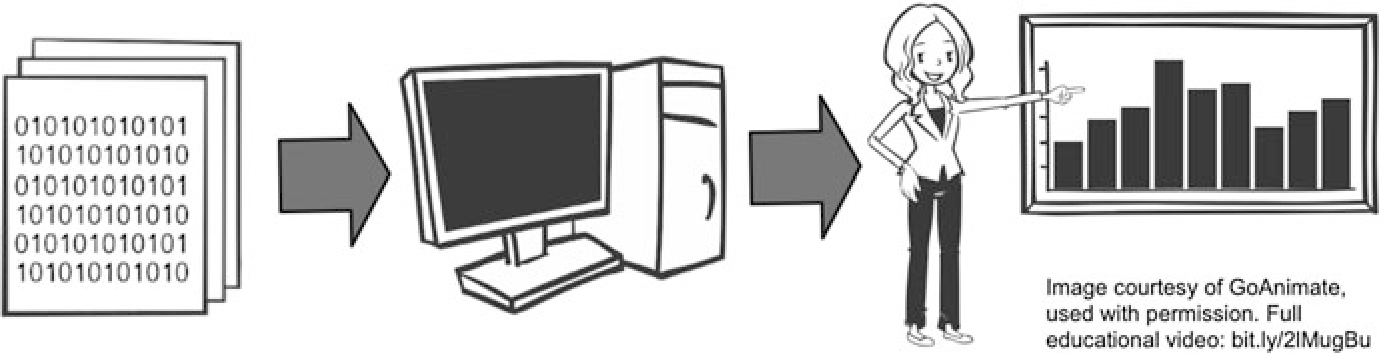
\includegraphics[width=.91\textwidth]{figures/ch01_unnumbered_workflow.png}\\[-.2em]
 {\footnotesize 图片由 GoAnimate 提供，经授权使用。完整教学视频：\url{https://bit.ly/2lMugBu}。}
\end{center}

\begin{sourcebox}
\kaishu 这一切都以计算效率和实际应用为重。其理念是：从理论上最优的方法出发，确保将其转化为快速、便于用户使用的工具。
\end{sourcebox}

过去十年间，靶向学习已经发展为构造效应估计量和预测函数的可靠框架。随着靶向学习不断发展，它不仅为许多数据结构中的现有问题提供了新的解决方法，也在不同应用领域带来了新的发现。相关研究涉及随机对照试验（randomized controlled trial）、由边际结构模型（marginal structural model）定义的参数、病例对照研究、协同 TMLE（collaborative TMLE）、缺失和删失数据、纵向数据（longitudinal data）、效应修饰、比较效果研究、衰老、癌症、职业暴露、医保计划支付风险调整以及 HIV 等。在许多情况下，这些研究将靶向学习技术与标准方法进行了比较，表明它在模拟研究和现实应用中具有更好的表现。

\section{传统估计方法的失效}
\label{sec:ch01-traditional-fail}

经典横断面研究已有许多可用的方法，例如传统参数回归和若干现成的统计机器学习技术；然而，对于数据科学各领域中的复杂纵向研究，相关方法却十分匮乏。这些方法在横断面研究中就会失效，其假设也会不成立；将它们用于涉及时变处理、网络或流式数据等复杂数据类型时，问题会进一步加剧。本书旨在弥补这一缺口，介绍为处理此类难题而专门设计的靶向学习方法。第一部《靶向学习》讨论了前述横断面研究方法，也介绍了最早用于纵向研究的 TMLE 估计量，展示了靶向学习方法在多种数据结构中的优势。本书进一步介绍新的进展，因此采用了《复杂纵向研究的因果推断》这一副标题。

人们还普遍认为，在非参数或半参数模型中，采用数据自适应的估计，也就是基于机器学习的估计时，无法进行统计推断。让我们更具体地说明这一点。假设在一项观察性研究中，我们已经使用机器学习，将临床结局的条件均值拟合为处理与患者特征的函数。为此，我们可以采用集成学习器（ensemble learner），例如超级学习器：它结合算法库中的多个算法，并依赖交叉验证（cross-validation）。然后，通过以下两步，将这一拟合结果映射为特定处理下均值（treatment-specific mean）的估计：（1）计算指定处理条件下的预测结局；（2）在样本的全部 $n$ 名研究对象中，对这些预测值取平均。

以往的常规做法并不是使用机器学习，而是根据参数回归模型，用极大似然估计量来估计回归函数。在这种情形下，所得特定处理下均值，是未知回归系数的极大似然估计量的一个简单函数。因此，如果回归模型设定正确，特定处理下均值的这一极大似然估计量就是渐近线性的（asymptotically linear）。（这意味着，该极大似然估计量减去真实的特定处理下均值，等于其影响曲线的经验均值再加上一个可忽略的余项。）由此，它近似服从正态分布，其均值为真实的特定处理下均值，方差为影响曲线的方差除以样本量。置信区间的构造与基于样本均值的置信区间类似。然而，在实际中，我们知道这一参数模型存在设定错误，因此，该极大似然估计量虽服从正态分布，却带有偏差，95\% 置信区间的渐近覆盖率将等于零。

如果像前面最初提出的那样使用机器学习算法，那么，特定处理下均值的估计量一般不服从正态分布，且偏差大于 $1/\sqrt{n}$。因此，用 $\sqrt{n}$ 标准化之后，估计量与其真值之差将趋于无穷！由于估计量的抽样分布通常无法用某个给定分布（例如正态分布）很好地近似，我们也就无法根据这样的极限分布进行统计推断。

值得注意的是，只要对基于机器学习的拟合结果作一个小幅的靶向修正，就可能使所得特定处理下均值的估计量具有渐近线性，且其影响曲线等于有效影响曲线（efficient influence curve）。这里的初始估计量（initial estimator）估计的是数据分布，或其相关部分，例如本例中的回归函数；将它代入目标参数（target parameter）时，所得估计量通常偏差过大，而且不服从正态分布。这一小幅修正能够把初始估计量映射为更新后的估计量，使相应的代入估计量近似无偏，并具有方差最小的正态极限分布。

% 原书第 6—11 页；第 1.3—1.4 节。
\section{靶向学习的实际应用}
\label{sec:ch01-in-practice}

在各种现实分析中，已有许多广受关注的例子展示了靶向学习的益处。例如，Pandora 的数据科学家采用靶向学习发现，流媒体音乐的播放使新发行音乐的销量提高了 2.3\%，使既有曲目销量提高了 2.7\%。《Billboard》杂志曾报道这项研究。医疗保健是应用靶向学习尤为频繁的一个领域。靶向学习如何改善医疗保健？在发表于《Lancet Respiratory Medicine》的研究中，研究人员为重症监护病房开发了一种预测死亡率的超级学习器，其表现优于疾病严重程度评分。临床医生可通过在线用户界面使用这一算法。在另一项发表于《World Psychiatry》的研究中，研究人员构建了一个新函数，用于预测创伤事件后的创伤后应激障碍（posttraumatic stress disorder，PTSD）。该算法的表现十分出色，96\% 的 PTSD 结局都落在预测值最高的 10\% 人群中。近期，一项计算卫生经济学分析利用大型健康记录理赔数据库，考察了单项病症对医疗总支出的影响。用于效应估计的靶向学习估计量，在控制人口学信息和其他病症后，按照各病症类别对医疗总支出的贡献对其排序。以往关于病症对医疗支出影响的研究，主要采用医保计划支付风险调整中的参数回归公式，或未经混杂因素调整的汇总均值。这项研究的结果表明，多发性硬化、充血性心力衰竭、重症癌症、重性抑郁和双相障碍，以及慢性肝炎，是费用最高的病症（见表 1.1）。相比之下，用于医保计划支付风险调整的参数回归公式，无论在效应估计值的大小，还是在相对排序上，都存在不可忽视的差异。如果现行风险调整公式未能准确反映各病症的增量效应，医疗保险机构挑选参保人的激励就可能继续存在。关于早期研究的其他参考文献，见第 1.6 节。

\begin{table}[htbp]
 \centering
 \caption{靶向学习效应估计值最高的五类病症及其参数回归估计值}
 \label{tab:ch01-cost-estimates}
 \begin{tabular}{lrr}
  \toprule
  病症 & 靶向学习 & 参数回归\\
  \midrule
  多发性硬化 & 67,011 & 30,715\\
  充血性心力衰竭 & 19,904 & 4131\\
  肺癌、脑癌及重症癌症 & 19,233 & 24,528\\
  重性抑郁与双相障碍 & 15,398 & 3498\\
  慢性肝炎 & 10,530 & 5539\\
  \bottomrule
 \end{tabular}
\end{table}

\section{统计估计问题}
\label{sec:ch01-statistical-estimation}

我们用一个简化的体外受精（in vitro fertilization，IVF）例子，介绍纵向统计估计问题。这里，我们在控制时变混杂因素（time-dependent confounder）的情况下，估计一项最多包含两个 IVF 周期的治疗计划获得成功的概率，即胚胎移植后活产的概率。不孕症是一个全球性的公共卫生问题，目前已有多种治疗方法可供选择。IVF 是一种日益普遍的治疗方法，但由于 IVF 治疗计划包含多个周期，要准确评价其成功率一直颇具挑战。

\subsection{数据}
\label{subsec:ch01-data}

考虑各时点 $t$（$t=0,\ldots,T+1$）的协变量（covariate）向量 $L_t$，其中，基线协变量记为 $L_0$。为了说明问题，我们将 IVF 研究限定为一种特定的数据结构，其中只有两个相继的时点接受干预。这一数据结构是横断面数据的简单扩展；横断面情形只在单个时点接受干预。

在这一数据结构中，各时点 $t$ 的协变量组成 $\bar L=(L_0,L_1,L_2)$，且 $T=1$。在序贯决策过程文献中，协变量集合 $\bar L$ 也称为状态集合；此外，也常使用 $L_{1:2}$ 之类的下标记号来表示协变量集合的某个特定子集。$L_0$ 中的协变量包括母亲年龄、IVF 机构、获卵数、移植或冷冻的胚胎数，以及妊娠指标。$L_1$ 和 $L_2$ 编码 IVF 周期是否成功。干预集合（也称为“行动”）记为 $\bar A=(A_0,A_1)$，其中随机变量 $A_t$ 表示时点 $t$ 的干预。在 IVF 研究中，$\bar A$ 中的每个 $A_t$ 都是二值变量，表示是否尝试了该 IVF 周期。按约定，如果 $A_t=0$，则 $L_{t+1}=0$；如果 $L_1=1$，则 $L_2=1$。

于是，我们可以把一名随机抽取的研究对象的数据表示为按时间排序的数据结构：
\[
 O=(L_0,A_0,L_1,A_1,L_2),
\]
其中，假定 $L_t$ 发生在 $A_t$ 之前。最终的测量值 $L_2$ 记为 $Y$，表示感兴趣的结局。为简便起见，我们考虑 $Y$ 为二值变量的情形。样本由随机变量 $O$ 的 $n$ 次独立同分布（independent and identically distributed，i.i.d.）抽样 $O_1,\ldots,O_n$ 构成。这些随机变量的实现值记为 $o_1,\ldots,o_n$。按照数据的时间顺序，$O$ 的概率分布可分解为
\[
 \begin{aligned}
 p(O)={}&p(L_0)\times p(L_1\mid A_0,L_0)
                \times p(Y\mid A_1,L_1,A_0,L_0)\\
        &{}\times p(A_0\mid L_0)\times p(A_1\mid L_1,A_0,L_0).
 \end{aligned}
\]

\subsection{模型与参数}
\label{subsec:ch01-model-parameter}

我们假设，观测数据的生成分布属于一个非参数统计模型 $\mathcal M$；这一模型包含可能的概率分布集合。感兴趣的参数，是一项最多包含两个 IVF 周期的治疗计划获得成功的概率，即胚胎移植后活产的概率，它可以写成
% 此处严格照录印刷原式：求和号无指标，第二因子为 L_1=1。
\[
 \begin{aligned}
 \Psi(P_0)=E_{P_0}\Bigl(&\sum P_0(Y=1\mid A_{0:1}=1,L_{0:1}=l_{0:1})\\
 &{}\times P_0(L_1=1\mid A_0=1,L_0=l_0)\Bigr).
 \end{aligned}
\]
在第 2 章将讨论的因果可识别性假设下，因果参数可以写为
\[
 P(Y_{(1,1)}=1),
\]
且等于 $\Psi(P_0)$，其中 $Y_{(1,1)}$ 是干预 $A_{0:1}=1$ 下的反事实结局（counterfactual outcome）。

\subsection{靶向最小损失估计量}
\label{subsec:ch01-tmle}

针对这一研究问题，可以构造靶向最小损失估计量（targeted minimum loss-based estimator，TMLE），以估计 $P(Y_{(1,1)}=1)$。TMLE 框架是一个极其一般的系统，由损失函数（loss function）、初始估计量，以及通过初始（或当前）估计量的最不利子模型（least favorable submodel）所定义。确切地说，它需要以下要素：
\begin{enumerate}
 \item 定义一个目标参数：它将观测单位数据结构的概率分布的一个参数（通常为无限维参数）映射到参数空间。
 \item 推导目标参数路径导数的有效影响曲线。
 \item 规定一个损失函数。
 \item 指定一个通过该参数的初始（或当前）估计量的最不利子模型，使扰动（fluctuation）为零时，基于损失的得分的线性张成空间包含有效影响曲线。
 \item 给出一个算法：对最不利参数子模型的扰动参数，迭代地最小化由指定损失函数定义的经验风险（empirical risk），并更新初始（或当前）估计量。
\end{enumerate}

这一迭代最小化过程一直进行到扰动参数的极大似然估计值接近零。根据子模型和损失函数所满足的广义基于损失的得分条件，所得无限维参数的 TMLE 满足有效得分方程（efficient score equation）。这为目标参数相应的代入估计量具有双重稳健性和渐近有效性（asymptotic efficiency）奠定了基础。靶向极大似然估计量是 TMLE 的一种。第 5 章将证明，总能选取一个最不利子模型，使得仅需对由指定损失函数定义的经验风险进行一次最小化，就足以求解有效得分方程。这些特殊的局部最不利子模型称为通用最不利子模型（universal least favorable submodel）。

\subsection{其他常见的估计问题}
\label{subsec:ch01-other-problems}

\noindent\textbf{特定规则下的均值（rule-specific mean）。}
在利用纵向观察数据研究临床问题时，我们常常希望评价随时间延续的处理规则，这类规则称为动态处理规则（dynamic rule），有时也称为处理策略或处理方案（regime 或 regimen）。从更广泛的数理科学视角来看，动态处理规则属于序贯决策理论。其中的一个关键点是：对于某个给定时点，如果考虑即时结局和考虑长期结局，最优的干预决策可能不同。这类决策在统计学中十分常见，尤其常见于医学和公共卫生问题，因此，估计最优动态处理规则的方法具有重要意义。所考虑的规则还可能包含复杂的分类器。例如，考虑美国既往未接受治疗的 HIV 感染者应在何时开始抗逆转录病毒治疗的问题。在这里，我们希望考虑一组预先指定的 CD4 计数阈值，例如从 $200$ 到 $500\ \text{细胞}/\mathrm{mm}^3$，每隔 $50$ 设置一个阈值；当 CD4 计数低于阈值时，就应开始抗逆转录病毒治疗。每个动态处理规则都以一个 CD4 阈值作为索引。

设 $\mathcal D=(d_1,\ldots,d_K)$ 是我们考虑的动态处理规则集合。每个动态处理规则 $d_k$ 编码一个按时间排列的规则序列 $d_{k,t}$（$t=1,\ldots,T$），其中，$d_{k,t}$ 表示将患者此前测得的协变量 $\bar L_t$ 映射为时点 $t$ 应接受的处理 $a(t)$ 的函数。在不会引起歧义时，为简化记号，我们省略单个规则 $d$ 的下标。如果某个个体实际接受的干预与规则 $d$ 指示的干预相同，就称该个体直到时点 $t$ 都遵循规则 $d$。设 $Y^d$ 表示假如令该研究对象在所有时点都遵循规则 $d$，本会观测到的（反事实）取值。我们的目标是确定最优动态处理规则 $d^*$，即 $\mathcal D$ 中使潜在结局（potential outcome）$Y^d$ 的期望值最大的规则。我们首先考虑这样一个估计问题：对每个规则 $d\in\mathcal D$，估计假如所有人都遵循规则 $d$ 时，$Y$ 的总体均值，即 $E(Y^d)$。由于本例数据结构中的 $Y$ 是二值变量，这也等于 $Y^d=1$ 的概率。在一组较强的可识别性假设下，包括无未测量混杂因素的假设，可以利用 g 计算公式（g-computation formula），将 $E(Y^d)$ 表示为观测数据生成分布 $P$ 的一个函数：
\[
 \begin{aligned}
 \Psi^d(P)={}&\sum_{l_0}\sum_{l_1}
 P\bigl(Y=1\mid A_1=d(\bar l_1),\bar L_1=\bar l_1,A_0=d(l_0)\bigr)\\
 &{}\times P\bigl(L_1=l_1\mid A_0=d(l_0),L_0=l_0\bigr)P(L_0=l_0).
 \end{aligned}
\]
我们在这里较为详细地说明动态处理规则的数据结构和统计估计问题，是因为第 2—4 章的多处内容将把这项研究作为贯穿的实例来讲解。

\medskip
\noindent\textbf{社区随机试验。}
在社区随机试验（community randomized trial）中，我们关心的是这样一种情形：将干预分配给少数几个社区，并从每个社区随机抽取个体样本，收集其协变量和结局数据。借助我们此前关于有偏抽样的研究，可以在这些试验中识别感兴趣的参数，例如因果对比。第 13 章将更详细地介绍这一数据结构。

\medskip
\noindent\textbf{网络。}
网络数据日益常见。从最初的疾病传播，到后来的电子邮件，再到如今迅速扩张的社交网络，我们经常观测到这样的总体：其中各个单位按照某种网络，在因果关系上相互连接。其数据结构通常是纵向的，包含时变暴露和协变量。第 20 章和第 21 章将更详细地介绍这些数据结构和参数。

% 原书第 11—14 页；第 1.5—1.6 节。
\section{靶向学习路线图}
\label{sec:ch01-roadmap}

本书前四章介绍纵向数据靶向学习的关键基础知识，包括靶向学习路线图，以及预测和因果推断中的估计问题（图 1.1）。这几章围绕数据结构 $O=(L_0,A_0,L_1,A_1,L_2)\sim P_0$、非参数统计模型 $\mathcal M$ 和因果参数 $\Psi^d(P)$，循序渐进地引导读者理解主要概念。本章说明了为什么需要新的方法来处理复杂的纵向数据科学问题，并介绍了数据、模型和目标参数。第 2—4 章将进一步阐释靶向学习路线图。

\begin{description}[leftmargin=0em,labelindent=0em,itemindent=0em,style=nextline,itemsep=.6em]
 \item[定义模型和目标参数。]
 结构因果模型（structural causal model，SCM）是对底层反事实结局数据建立的模型，表示在理想实验中本会生成的数据。它将关于数据生成过程的知识转化为因果假设。SCM 也生成观测数据 $O$，使我们能够确定：为了从观测数据中识别因果效应，还需要哪些额外假设。
 \item[用于预测的超级学习。]
 我们需要能够从复杂数据中学习的灵活估计量，并将介绍适用于纵向结构的集成超级学习。超级学习既可以融入效应估计，也可以作为处理预测问题的独立工具。预先掌握一些交叉验证和机器学习知识将有所帮助，例如第一部《靶向学习》第 3 章介绍的内容。
 \item[TMLE。]
 通过 TMLE，我们能够针对感兴趣的参数，而非整个概率分布 $P_0$，进行最优的偏差—方差权衡，从而将估计靶向于（因果）效应参数。这些估计量具有许多理想的统计性质；在某些情形下，对于一些复杂参数，它们还是唯一可用的估计量。
\end{description}

这段简短的预告旨在为后续章节提供指引，让读者预先了解我们将走向何处、路线图的各个环节如何衔接，以及为什么按照这样的先后顺序安排内容。

\begin{figure}[p]
 \centering
 % 图 1.1：逐项依据原书第 12 页重绘。
\begin{tikzpicture}[
 x=1cm,y=1cm,
 ch01roadbox/.style={draw=black!75,rounded corners=2pt,line width=.6pt,
   text width=12.25cm,align=center,font=\footnotesize,
   inner xsep=7pt,inner ysep=6pt},
 ch01roadarrow/.style={-{Stealth[length=2.5mm,width=1.8mm]},line width=.7pt},
 ch01side/.style={font=\small\bfseries,align=center,inner sep=0pt}
]
\node[ch01roadbox] (ch01data) {%
 \textbf{数据}\\
 数据是随机变量 $O$ 的 $n$ 次观测。\\
 $O$ 的概率分布为 $P_0$。};
\node[ch01roadbox,below=.55cm of ch01data] (ch01model) {%
 \textbf{模型}\\
 统计模型 $\mathcal M$ 是 $O$ 的可能概率分布的集合，$P_0\in\mathcal M$。\\
 模型是在 $P_0$ 的统计模型基础上，可能进一步加入\\
 不可检验的因果假设而得到的。};
\node[ch01roadbox,below=.55cm of ch01model] (ch01target) {%
 \textbf{目标参数}\\
 参数 $\Psi(P_0)$ 是 $P_0$ 的一个特定特征，其中 $\Psi$ 将概率分布 $P_0$\\
 映射为感兴趣的目标参数。};
\node[ch01roadbox,below=.55cm of ch01target] (ch01super) {%
 \textbf{超级学习器}\\
 估计过程的第一步通常是利用机器学习算法——超级学习器，\\
 对 $P_0$ 的相关部分得到一个或多个初始估计。};
\node[ch01roadbox,below=.55cm of ch01super] (ch01tmle) {%
 \textbf{靶向最小损失估计}\\
 利用超级学习获得数据生成分布相关部分的初始估计后，\\
 TMLE 的第二阶段通过一个靶向步骤更新这些初始拟合，\\
 使感兴趣的参数达到最优的偏差—方差权衡。};
\node[ch01roadbox,below=.55cm of ch01tmle] (ch01inference) {%
 \textbf{推断}\\
 利用影响曲线或基于重抽样的方法计算目标参数估计量的标准误，\\
 以评价估计量的不确定性。};
\node[ch01roadbox,below=.55cm of ch01inference] (ch01interpret) {%
 \textbf{解释}\\
 目标参数可解释为纯粹的统计参数，也可在模型中可能进一步\\
 加入不可检验假设的条件下，解释为因果参数。};

\draw[ch01roadarrow] (ch01data.south) -- (ch01model.north);
\draw[ch01roadarrow] (ch01model.south) -- (ch01target.north);
\draw[ch01roadarrow] (ch01target.south) -- (ch01super.north);
\draw[ch01roadarrow] (ch01super.south) -- (ch01tmle.north);
\draw[ch01roadarrow] (ch01tmle.south) -- (ch01inference.north);
\draw[ch01roadarrow] (ch01inference.south) -- (ch01interpret.north);

\draw[draw=black!75,rounded corners=2pt,line width=.6pt]
 ($(ch01data.north west)+(-1.0,0)$) rectangle
 ($(ch01target.south west)+(-.25,0)$);
\node[ch01side] at
 ($(ch01data.north west)!.5!(ch01target.south west)+(-.625,0)$)
 {\shortstack{界\\定\\研\\究\\问\\题}};
\draw[draw=black!75,rounded corners=2pt,line width=.6pt]
 ($(ch01super.north west)+(-1.0,0)$) rectangle
 ($(ch01tmle.south west)+(-.25,0)$);
\node[ch01side] at
 ($(ch01super.north west)!.5!(ch01tmle.south west)+(-.625,0)$)
 {\shortstack{估\\计}};
\draw[draw=black!75,rounded corners=2pt,line width=.6pt]
 ($(ch01inference.north west)+(-1.0,0)$) rectangle
 ($(ch01interpret.south west)+(-.25,0)$);
\node[ch01side] at
 ($(ch01inference.north west)!.5!(ch01interpret.south west)+(-.625,0)$)
 {\shortstack{推\\断}};
\end{tikzpicture}

 \caption{靶向学习路线图}
 \label{fig:ch01-roadmap}
\end{figure}
\FloatBarrier

\section{注记与延伸阅读}
\label{sec:ch01-notes}

本章开篇以 Google Flu Trends 和 Netflix Prize 为例，介绍现实数据科学所面临的挑战。关于 Google Flu Trends 的历史，可参阅《Wired》杂志的文章（Lazer and Kennedy，2015）；Netflix Prize 的背景则见《Forbes》的报道（Holiday，2012）。七年前出版的第一部《靶向学习》提供了这一领域至关重要的基础知识（van der Laan and Rose，2011）。

第 1.1 节讨论了靶向学习方法为现有问题提供新解决方法的诸多领域。各领域的具体参考文献如下：随机对照试验（Rubin and van der Laan，2008；Moore and van der Laan，2009a,b,c；Rosenblum and van der Laan，2009）；由边际结构模型定义的参数（Rosenblum and van der Laan，2010a）；病例对照研究（van der Laan，2008a；Rose and van der Laan，2008，2009，2014a,b）；协同 TMLE（van der Laan and Gruber，2010；Gruber and van der Laan，2010a；Stitelman and van der Laan，2010）；缺失和删失数据（Stitelman and van der Laan，2010；Rose and van der Laan，2011）；效应修饰（Polley and van der Laan，2009；Stitelman and van der Laan，2011）；纵向数据（van der Laan，2010a；van der Laan and Gruber，2012）；网络（van der Laan，2014a）；基于社区的干预（van der Laan，2010c）；比较效果研究（Neugebauer et al.，2014a；Kunz et al.，2017）；生物标志物与基因组学中的变量重要性（Bembom et al.，2009；Wang et al.，2011a,b，2014；Tuglus and van der Laan，2011；Wang and van der Laan，2011）；衰老（Bembom and van der Laan，2007；Rose，2013）；癌症（Polley and van der Laan，2009）；职业暴露（Chambaz et al.，2014）；卫生经济学（Rose，2016；Rose et al.，2017；Shrestha et al.，2018）；以及 HIV（Rosenblum et al.，2009）。Rose et al.（2017）的论文，也是将靶向学习框架应用于算法公平性、问责性和透明度的一个例子。他们表明，即使已有针对既往疾病的保护措施，保险机构仍可能借助药品理赔数据和集成机器学习，识别“无利可图”的参保人，然后针对这些人促使其退保。算法在社会中的应用日益广泛，也带来广泛的风险，例如数据中通常就内含偏差。关于刑事司法改革中算法公平性的简要介绍，可参阅 Lum（2017）。

第 1.3 节概述的计算卫生经济学项目，在其他文献中有详细讨论（Rose，2018）。该节介绍的研究论文包括 Peoples（2014）、Pirracchio et al.（2015）和 Kessler et al.（2014）。面向公共卫生应用读者的另一篇教程，介绍了单时点处理且结局为连续变量时的 TMLE（Schuler and Rose，2017）。对于二值结局，可参阅《靶向学习》（2011）第 4 章。

第 1.2 节讨论了机器学习情境下的推断问题，以及靶向学习如何克服这些不足。这里再补充一些背景，特别说明为什么用自助法对机器学习进行推断时可能失效。非参数自助法利用从经验分布（empirical distribution）中抽样时估计量的抽样分布，来估计原估计量的抽样分布。也就是说，我们用经验分布估计数据分布，并希望经验分布向真实数据分布的收敛，能够转化为估计量抽样分布的收敛。如果估计量的抽样分布仅依赖于数据分布的光滑函数，那么，这种方法应当能够很好地发挥作用；但如果它在本质上依赖于数据分布的密度，就可能失效，因为离散的经验分布对该密度的估计很差。事实上，如果估计量是经验概率分布的一个具有良好可微性（即所谓 Hadamard 可微性或紧可微性）的泛函，那么，非参数自助法就是估计其抽样分布的有效且一致的方法（Gill，1989；van der Vaart and Wellner，1996）。另一方面，依赖平滑、模型选择、交叉验证或其他形式机器学习的估计量，根本不是数据的 Hadamard 可微泛函，因此可以预期，非参数自助法会不一致。


% 第 2 章；各分文件依原书次序汇总。
% 原书第 15—18 页；章首导言、关键定义与第 2.1 节。
\chapter{定义模型与参数}
\label{ch:defining-model-parameter}
\chapterauthors{Sherri Rose 与 Mark J. van der Laan}
\chapteraffiliations{%
S. Rose（通讯作者）：美国哈佛医学院卫生保健政策系，180 Longwood Ave, Boston, MA 02115, USA；电子邮箱：\href{mailto:rose@hcp.med.harvard.edu}{rose@hcp.med.harvard.edu}。\\
M. J. van der Laan：美国加利福尼亚大学伯克利分校生物统计学部及统计学系，101 Haviland Hall, \#7358, Berkeley, CA 94720, USA；电子邮箱：\href{mailto:laan@berkeley.edu}{laan@berkeley.edu}。\\
本章 DOI：\url{https://doi.org/10.1007/978-3-319-65304-4_2}。}

在数据科学中，我们常常希望估计因果效应（causal effect），并评价估计量的不确定性。第 1 章介绍了这样一条路线：针对现实研究问题，在复杂数据类型中估计因果效应。本章将详细给出模型和目标参数（target parameter）的形式化定义；它们会随具体研究问题而变化。不过，这里介绍的概念将贯穿全书，适用于多种参数，而所用的基本模板具有一般性。

我们建议读者在阅读本章之前，先熟悉因果推断（causal inference）的基本概念，例如阅读 Judea Pearl 的《因果论》（\emph{Causality}）第 2 版（Pearl，2009a）。第一部《靶向学习》（\emph{Targeted Learning}）第 2 章，针对单时点处理的数据结构和平均处理效应（average treatment effect，ATE）参数，概括了 Pearl 著作中的关键内容；与 Pearl 的书相比，这是一份更为简短的背景材料。本章不会重复全部基础知识，但会提供处理我们所关注的复杂因果问题所必需的内容。读者需要从本章掌握的一个关键认识是：因果推断既需要一个因果模型，将因果效应定义为数据分布的目标参数，也需要稳健的半参数有效估计。本书几乎完全聚焦于后者，也就是估计；而 Pearl 的工作主要聚焦于前者。

\begin{sourcebox}[关键定义与记号]
\begin{itemize}[leftmargin=1.5em,itemsep=.15em,topsep=.2em]
 \item 统计模型（statistical model）$\mathcal M$ 是一组可能的概率分布 $P$ 的集合。
 \item $P_0$ 是 $O$ 的真实分布。
 \item 定义目标参数，需要指定一个作用于 $P_0$ 的映射 $\Psi$。$\Psi$ 将任意 $P\in\mathcal M$ 映射为数值向量 $\Psi(P)$。对于 $d$ 维参数，这一映射记为 $\Psi\colon\mathcal M\to\mathbb R^d$。
 \item $\psi_0$ 是 $\Psi(P_0)$ 的取值，即参数的真值。
\end{itemize}
统计估计问题，就是将观测数据 $O_1,\ldots,O_n$ 映射为 $\Psi(P_0)$ 的一个估计量，在估计中纳入 $P_0\in\mathcal M$ 这一知识，并同时评价估计量的不确定性。

{\kaishu 更多背景知识见《靶向学习》（2011）第 2 章。}
\end{sourcebox}

数据 $O_1,\ldots,O_n$ 由随机变量 $O$ 的 $n$ 个独立同分布（independent and identically distributed，i.i.d.）副本组成，$O$ 的真实概率分布为 $P_0$。对于第 1 章的数据结构，例如
\[
 O=(L_0,A_0,L_1,A_1,L_2=Y),
\]
其中，$L_{0:1}$ 是协变量（covariate）向量，$A_{0:1}$ 是干预（intervention）向量，$L_2=Y$ 是结局。大写字母表示随机变量，小写字母则表示相应变量的某个具体取值。当所有变量都是离散变量时，$P_0(L_0=l_0,A_0=a_0,L_1=l_1,A_1=a_1,Y=y)$ 为 $O=(L_0,A_0,L_1,A_1,Y)$ 的每种可能结果 $(l_0,a_0,l_1,a_1,y)$ 指定一个概率。

接下来，我们将在统计模型所依据的最小假设基础上，加入不可检验的因果假设，从而定义一个模型。这样，我们既能定义一个具有因果解释的感兴趣参数，也能确定：为了从观测数据分布中识别这一因果参数，究竟需要哪些假设。最后，我们将选定统计模型与目标参数。

\section{定义结构因果模型}
\label{sec:ch02-scm}

我们考虑一组内生变量（endogenous variable）$X=(X_j:j)$。对于这些变量，结构因果模型（structural causal model，SCM）将其定义为其他内生变量与外生误差（exogenous error）的确定性函数。外生变量（exogenous variable）记为 $U=(U_{X_j}:j)$，它们从不被观测。对于每个 $X_j$，我们在其他 $X$ 变量中指定 $X_j$ 的父节点（parent）$\operatorname{Pa}(X_j)$。内生变量 $X$ 往往包含可观测变量 $O$，但也可能包含不可观测变量。我们假设，每个 $X_j$ 都是 $\operatorname{Pa}(X_j)$ 与一个外生变量 $U_{X_j}$ 的函数：
\[
 X_j=f_{X_j}\bigl(\operatorname{Pa}(X_j),U_{X_j}\bigr),
 \qquad j=1\ldots,J.
\]

函数 $f_{X_j}$ 与 $U$ 的联合分布共同确定 $(U,X)$ 的数据生成分布（data-generating distribution）：它们描述了一个由结构方程构成的确定性系统，将 $U$ 的一个实现值确定地映射为 $X$ 的一个实现值。这些函数 $f_{X_j}$ 以及 $U$ 的联合分布可以不作具体限定；也可能因为具备领域知识，而愿意对它们作出更强的限制。我们的知识通常不足以支持一个完全参数化的 SCM。

\begin{sourcebox}
\textbf{SCM 是随机变量 $(U,X)$ 的一个统计模型。}
通过以下两方面的变化，可以定义 $(U,X)$ 的所有可能数据生成分布的集合：
\begin{enumerate}[itemsep=.15em,topsep=.2em]
 \item 令函数集 $f=(f_{X_j}:j)$ 在所有允许的函数形式中变化；
 \item 令误差 $U$ 的分布在所有可能的误差分布中变化。
\end{enumerate}
\end{sourcebox}

在第 1 章讨论的体外受精（in vitro fertilization，IVF）研究，以及何时开始 HIV 治疗的研究中，$j=1,\ldots,J$，其中 $J=5$，且 $X$ 中的所有变量均可观测。因此，$X=(X_1,X_2,X_3,X_4,X_5)$。我们再将 $X$ 改写为 $X=(L_0,A_0,L_1,A_1,Y)$，其中 $X_1=L_0$、$X_2=A_0$、$X_3=L_1$、$X_4=A_1$、$X_5=Y$。向量 $L_0$ 和 $L_1$ 可以同时包含二值变量和连续变量；而在两个例子中，$A_0$、$A_1$ 和 $Y$ 都是二值变量。我们需要明确指出，这些变量按如下时间顺序生成：
\[
 L_0\to A_0\to L_1\to A_1\to Y.
\]

具体来看 IVF 研究。首先测量基线变量 $L_0$，包括母亲年龄、IVF 机构、获卵数、移植或冷冻的胚胎数，以及妊娠指标。随后依次出现 $A_0$，表示是否尝试了一个 IVF 周期；接着出现 $L_1$，表示该 IVF 周期是否成功。$A_1$ 在 $L_1$ 之后出现，表示是否尝试了第二个 IVF 周期；最后出现 $Y$，表示在 $L_1$ 时尝试的 IVF 周期中是否至少有一次成功。回顾前面的约定：如果 $A_t=0$，则 $L_{t+1}=0$；如果 $L_1=1$，则 $Y=1$。因此，我们有函数 $f=(f_{L_0},f_{A_0},f_{L_1},f_{A_1},f_Y)$ 和外生变量 $U=(U_{L_0},U_{A_0},U_{L_1},U_{A_1},U_Y)$。结构方程模型为
% 原书 A_1 方程的误差下标印为 A_0，照录而不改为 A_1。
\begin{equation}
 \begin{aligned}
 L_0&=f_{L_0}(U_{L_0}),\\
 A_0&=f_{A_0}(L_0,U_{A_0}),\\
 L_1&=f_{L_1}(L_0,A_0,U_{L_1}),\\
 A_1&=f_{A_1}(L_0,A_0,L_1,U_{A_0}),\\
 Y&=f_Y(L_0,A_0,L_1,A_1,U_Y).
 \end{aligned}
 \tag{2.1}
\end{equation}
我们不对 $f_{L_0}$、$f_{A_0}$、$f_{L_1}$、$f_{A_1}$ 和 $f_Y$ 的函数形式作限制性假设；这些函数 $f$ 是非参数的。此外，本研究还假设不存在未测量的混杂因素（no unmeasured confounders）。确切地说，在式 (2.1) 中，我们假设数据按以下过程生成：
\begin{enumerate}
 \item 从概率分布 $P_U$ 抽取 $U$，并确保给定 $L_{0:1}$ 时，$U_{A_{0:1}}$ 与 $U_Y$ 独立。
 \item 将 $L_0$ 生成为 $U_{L_0}$ 的确定性函数。
 \item 将 $A_0$ 生成为 $L_0$ 和 $U_{A_0}$ 的确定性函数。
 \item 将 $L_1$ 生成为 $L_0$、$A_0$ 和 $U_{L_1}$ 的确定性函数。
 \item 将 $A_1$ 生成为 $L_0$、$A_0$、$L_1$ 和 $U_{A_1}$ 的确定性函数。
 \item 将 $Y$ 生成为 $L_0$、$A_0$、$L_1$、$A_1$ 和 $U_Y$ 的确定性函数。
\end{enumerate}

我们假定，观测数据结构 $O=(L_0,A_0,L_1,A_1,Y)$ 是上述系统中结构方程所生成的内生变量 $(L_0,A_0,L_1,A_1,Y)$ 的一个实现值；由此定义 $O$ 的 SCM。

SCM 表示我们根据对数据生成方式的认识而作出的一组不可检验的因果假设。第一部《靶向学习》（2011）的入门内容曾讨论单时点干预的 SCM。如那里所述，$O$ 的 SCM 还涉及界定随机变量 $(U,X)$ 与 $O$ 的关系，使完整数据的 SCM 能够用 $f$ 和 $U$ 的分布 $P_U$，对 $O$ 的概率分布进行参数化。在完整数据的 SCM 中，$(U,X)$ 的每个可能概率分布 $P_{U,X}$，都由所选择的误差分布 $P_U$ 和一组确定性函数 $(f_{X_j}:j)$ 来索引，并导出 $O$ 的一个概率分布 $P(P_{U,X})$。因此，完整数据的 SCM 能够利用 $(U,X)$ 的真实概率分布，对 $O$ 的真实概率分布进行参数化。于是，$O$ 的分布 $P_0$ 的统计模型 $\mathcal M$ 可以表示为 $\mathcal M=\{P(P_{U,X}):P_{U,X}\}$，其中，$P_{U,X}$ 在 SCM 所允许的 $(U,X)$ 的全部概率分布中变化。如果这一 $\mathcal M$ 是非参数的，那么，SCM 所编码的因果假设没有一个能用观测数据检验。

如果研究对象是被随机分配接受 IVF 治疗的，那么，结构方程模型可能为
% 式 (2.2) 及原书紧随文字均使用 U_{A_0}，与图 2.2 的标签分别照录。
\begin{equation}
 \begin{aligned}
 L_0&=f_{L_0}(U_{L_0}),\\
 A_0&=f_{A_0}(U_{A_0}),\\
 L_1&=f_{L_1}(L_0,A_0,U_{L_1}),\\
 A_1&=f_{A_1}(A_0,U_{A_0}),\\
 Y&=f_Y(L_0,A_0,L_1,A_1,U_Y).
 \end{aligned}
 \tag{2.2}
\end{equation}
在式 (2.2) 中，$A_0$ 仅为 $U_{A_0}$ 的确定性函数，$A_1$ 则仅为 $A_0$ 和 $U_{A_0}$ 的确定性函数。我们假定的这一随机化设计依赖此前的处理，但不依赖其他外生变量。虽然本书主要关注没有随机化的观察性研究（observational study），靶向学习（targeted learning）框架却具有相当广泛的适用性；第三编有三章专门讨论随机试验。

% 原书第 19—20 页；第 2.2 节及三幅因果图。
\section{因果图}
\label{sec:ch02-causal-graphs}

上一节将 SCM 介绍为一种系统的方法：从随机输入出发，为一组变量赋值，界定所需的因果假设，并评价因果目标参数的可识别性（identifiability）。因果图（causal graph）则是另一种常用表示方法，可以表达 SCM 所编码的部分假设。本书所有的因果图都是有向无环图（directed acyclic graph，DAG）：连接节点的边仅有一个箭头，而且不存在闭合回路。然而，面对纵向数据（longitudinal data）、网络及其他复杂数据结构时，这种表示方式很快就会在视觉上变得复杂。上一节的非参数结构方程没有这一缺点，因此，在某些情形下可能更为合适。此外，因果图并不针对某个特定的感兴趣目标参数，因而，由因果图得到的可识别性假设可能强于实际所需。

我们先在图 2.1 中给出式 (2.1) 的一种可能因果图。通过为每个 $X_j$ 定义 $\operatorname{Pa}(X_j)$，并定义联合分布 $P_U$，我们作出因果假设。根据 $f$ 所给出的关系，从 $\operatorname{Pa}(X_j)$ 中的每个节点向 $X_j$ 画有向箭头，并从每个 $U_{X_j}$ 向对应的 $X_j$ 画有向箭头。理想情况下，这些假设应以我们关于感兴趣科学问题的领域知识为依据。直接效应（direct effect），例如 $L_0$ 对 $L_1$ 的直接效应，由两个节点之间的有向箭头表示。如果不确定两个变量之间是否存在直接效应，我们默认将其包含在内，因为明确省略某个箭头，就意味着已知该直接效应不存在。例如，图 2.2 给出了 SCM (2.2) 的一种可能因果图。根据关于 SCM 中随机化的先验知识，我们明确省略了 $L_0$ 与 $A_0$ 之间以及 $L_1$ 与 $A_1$ 之间的有向箭头。

\begin{figure}[htbp]
 \centering
 % 图 2.1；依据原书第 19 页的实线箭头逐条重绘。
\begin{tikzpicture}[causal,x=1.7cm,y=1.3cm,
 ch02n/.style={inner sep=2pt,fill=white,font=\normalsize}]
\node[ch02n] (ch02aL0) at (0,0) {$L_0$};
\node[ch02n] (ch02aA0) at (1,1) {$A_0$};
\node[ch02n] (ch02aL1) at (2,0) {$L_1$};
\node[ch02n] (ch02aA1) at (3,1) {$A_1$};
\node[ch02n] (ch02aY) at (4,0) {$Y$};
\node[ch02n] (ch02aUL0) at (0,-1) {$U_{L_0}$};
\node[ch02n] (ch02aUA0) at (1,2) {$U_{A_0}$};
\node[ch02n] (ch02aUL1) at (2,-1) {$U_{L_1}$};
\node[ch02n] (ch02aUA1) at (3,2) {$U_{A_1}$};
\node[ch02n] (ch02aUY) at (4,-1) {$U_Y$};
\begin{scope}[on background layer]
\draw[ed] (ch02aUL0) -- (ch02aL0);
\draw[ed] (ch02aUA0) -- (ch02aA0);
\draw[ed] (ch02aUL1) -- (ch02aL1);
\draw[ed] (ch02aUA1) -- (ch02aA1);
\draw[ed] (ch02aUY) -- (ch02aY);
\draw[ed] (ch02aL0) -- (ch02aA0);
\draw[ed] (ch02aL0) -- (ch02aL1);
\draw[ed] (ch02aA0) -- (ch02aL1);
\draw[ed] (ch02aA0) -- (ch02aA1);
\draw[ed] (ch02aA0) -- (ch02aY);
\draw[ed] (ch02aL1) -- (ch02aA1);
\draw[ed] (ch02aL1) -- (ch02aY);
\draw[ed] (ch02aA1) -- (ch02aY);
\end{scope}
\end{tikzpicture}

 \caption{式 (2.1) 的一种可能因果图}
 \label{fig:ch02-causal-21}
\end{figure}

\begin{figure}[htbp]
 \centering
 % 图 2.2；保留源图 U_{A_1} -> A_1，不据式 (2.2) 擅改节点。
\begin{tikzpicture}[causal,x=1.7cm,y=1.3cm,
 ch02n/.style={inner sep=2pt,fill=white,font=\normalsize}]
\node[ch02n] (ch02bL0) at (0,0) {$L_0$};
\node[ch02n] (ch02bA0) at (1,1) {$A_0$};
\node[ch02n] (ch02bL1) at (2,0) {$L_1$};
\node[ch02n] (ch02bA1) at (3,1) {$A_1$};
\node[ch02n] (ch02bY) at (4,0) {$Y$};
\node[ch02n] (ch02bUL0) at (0,-1) {$U_{L_0}$};
\node[ch02n] (ch02bUA0) at (1,2) {$U_{A_0}$};
\node[ch02n] (ch02bUL1) at (2,-1) {$U_{L_1}$};
\node[ch02n] (ch02bUA1) at (3,2) {$U_{A_1}$};
\node[ch02n] (ch02bUY) at (4,-1) {$U_Y$};
\begin{scope}[on background layer]
\draw[ed] (ch02bUL0) -- (ch02bL0);
\draw[ed] (ch02bUA0) -- (ch02bA0);
\draw[ed] (ch02bUL1) -- (ch02bL1);
\draw[ed] (ch02bUA1) -- (ch02bA1);
\draw[ed] (ch02bUY) -- (ch02bY);
\draw[ed] (ch02bL0) -- (ch02bL1);
\draw[ed] (ch02bA0) -- (ch02bL1);
\draw[ed] (ch02bA0) -- (ch02bA1);
\draw[ed] (ch02bA0) -- (ch02bY);
\draw[ed] (ch02bL1) -- (ch02bY);
\draw[ed] (ch02bA1) -- (ch02bY);
\end{scope}
\end{tikzpicture}

 \caption{式 (2.2) 的一种可能因果图}
 \label{fig:ch02-causal-22}
\end{figure}

% 本段源书把前文定义为外生的 U 称为 endogenous；此处保留原文用词，详见校对报告。
图 2.1 和图 2.2 都没有在内生误差 $U=(U_{L_0},U_{A_0},U_{L_1},U_{A_1},U_Y)$ 之间画出任何箭头。这表明，式 (2.1) 和式 (2.2) 已经编码了一个关于内生误差联合独立性的强假设。然而，实践中我们不太可能作出这一假设。当希望反映内生变量 $U$ 之间的关系时，我们用虚线双向箭头来表示。如果对式 (2.1) 中 $P_U$ 的分布不作任何假设，所得因果图就如图 2.3 所示。该图中，处理节点与结局 $Y$ 之间有许多所谓的后门路径（backdoor path）。为了分离出感兴趣的因果效应，我们必须阻断从 $A_{0:1}$ 到 $Y$ 的所有尚未被阻断的后门路径。

\begin{figure}[htbp]
 \centering
 % 图 2.3；与图 2.1 相同的 13 条实线有向边，及五个 U 节点间的 10 条虚线双向边。
\begin{tikzpicture}[causal,x=1.7cm,y=1.3cm,
 ch02n/.style={inner sep=2.2pt,fill=white,font=\normalsize},
 ch02dep/.style={<->,line width=.45pt,dash pattern=on 4pt off 4pt}]
\node[ch02n] (ch02cL0) at (0,0) {$L_0$};
\node[ch02n] (ch02cA0) at (1,1) {$A_0$};
\node[ch02n] (ch02cL1) at (2,0) {$L_1$};
\node[ch02n] (ch02cA1) at (3,1) {$A_1$};
\node[ch02n] (ch02cY) at (4,0) {$Y$};
\node[ch02n] (ch02cUL0) at (0,-1) {$U_{L_0}$};
\node[ch02n] (ch02cUA0) at (1,2) {$U_{A_0}$};
\node[ch02n] (ch02cUL1) at (2,-2) {$U_{L_1}$};
\node[ch02n] (ch02cUA1) at (3,2) {$U_{A_1}$};
\node[ch02n] (ch02cUY) at (4,-1) {$U_Y$};
\begin{scope}[on background layer]
\draw[ed] (ch02cUL0) -- (ch02cL0);
\draw[ed] (ch02cUA0) -- (ch02cA0);
\draw[ed] (ch02cUL1) -- (ch02cL1);
\draw[ed] (ch02cUA1) -- (ch02cA1);
\draw[ed] (ch02cUY) -- (ch02cY);
\draw[ed] (ch02cL0) -- (ch02cA0);
\draw[ed] (ch02cL0) -- (ch02cL1);
\draw[ed] (ch02cA0) -- (ch02cL1);
\draw[ed] (ch02cA0) -- (ch02cA1);
\draw[ed] (ch02cA0) -- (ch02cY);
\draw[ed] (ch02cL1) -- (ch02cA1);
\draw[ed] (ch02cL1) -- (ch02cY);
\draw[ed] (ch02cA1) -- (ch02cY);
% 每一对误差节点恰有一条双向边；曲率仅为排版调整。
\draw[ch02dep] (ch02cUA0.north east)
 .. controls (1.5,2.4) and (2.5,2.4) .. (ch02cUA1.north west);
\draw[ch02dep] (ch02cUA0.west)
 .. controls (-1.1,2.15) and (-1.35,.1) .. (ch02cUL0.west);
\draw[ch02dep] (ch02cUA0.west)
 .. controls (-2.2,.65) and (-1.8,-2.8) .. (ch02cUL1.west);
\draw[ch02dep] (ch02cUA0.north east)
 .. controls (5.3,4.7) and (5.55,.3) .. (ch02cUY.north east);
\draw[ch02dep] (ch02cUA1.north west)
 .. controls (-1.3,4.7) and (-1.55,.3) .. (ch02cUL0.north west);
\draw[ch02dep] (ch02cUA1.east)
 .. controls (6.2,.65) and (5.8,-2.8) .. (ch02cUL1.east);
\draw[ch02dep] (ch02cUA1.east)
 .. controls (5.1,2.15) and (5.35,.1) .. (ch02cUY.east);
\draw[ch02dep] (ch02cUL0.south east)
 .. controls (.55,-1.65) and (1.35,-2.1) .. (ch02cUL1.west);
\draw[ch02dep] (ch02cUL1.east)
 .. controls (2.65,-2.1) and (3.45,-1.65) .. (ch02cUY.south west);
\draw[ch02dep] (ch02cUL0.south east)
 .. controls (1,-2.95) and (3,-2.95) .. (ch02cUY.south west);
\end{scope}
\end{tikzpicture}

 \caption{对 $P_U$ 的分布不作任何假设时，式 (2.1) 的因果图}
 \label{fig:ch02-causal-23}
\end{figure}
\FloatBarrier

% 原书第 21—22 页；第 2.3 节导言及第 2.3.1—2.3.2 小节。
\section{定义因果目标参数}
\label{sec:ch02-causal-target}

有了描述数据生成机制（data-generating mechanism）的 SCM，现在我们进一步定义因果目标参数。确切地说，我们将其定义为 SCM 中完整数据（full data）$(U,X)$ 的分布的一个参数。形式上，将完整数据 $(U,X)$ 的 SCM 记为 $\mathcal M^F$，它是 SCM 所描述的一组可能分布 $P_{U,X}$ 的集合。作为完整数据的模型，$\mathcal M^F$ 收集了底层数据 $(U,X)$ 的所有可能分布。$\Psi^F$ 是作用于 $P_{U,X}$ 的映射，所得 $\Psi^F(P_{U,X})$ 就是 $P_{U,X}$ 的目标参数。对于在所设定 SCM 编码的假设下，$(U,X)$ 的每一个可能分布 $P_{U,X}$，都需要定义这一映射。因此，我们写为 $\Psi^F\colon\mathcal M^F\to\mathbb R^d$，其中，$\mathbb R^d$ 表示参数是由 $d$ 个实数组成的向量。SCM $\mathcal M^F$ 包含的分布，由确定性函数 $f=(f_{X_j}:j)$ 和 $U$ 的分布 $P_U$ 索引；而 $f$ 和这一联合分布 $P_U$，都可以从完整数据 $(U,X)$ 的分布中识别。因此，目标参数也可以表示为 $f$ 与 $U$ 的联合分布的函数。

对于 IVF 研究，观测数据为 $O=(L_0,A_0,L_1,A_1,Y)$，SCM 由式 (2.1) 给出，且不对分布 $P_U$ 作任何假设。我们可以定义随机变量 $Y_{a_{0:1}}=f_Y(L_0,a_0,L_1,a_1,U_Y)$，对应于 SCM 中的干预 $A_{0:1}=a_{0:1}$。$Y_{a_{0:1}}$ 的边缘概率分布为
\[
 P_{U,X}(Y_{a_{0:1}}=y)
 =P_{U,X}\bigl(f_Y(L_0,a_0,L_1,a_1,U_Y)=y\bigr).
\]
回顾第 1 章给出的感兴趣统计参数：
% 本式与第 1 章原式一致：求和号不补下标，L_1=1 不改为 L_1=l_1。
\[
 \begin{aligned}
 \Psi(P_0)=E_{P_0}\Bigl(&\sum P_0(Y=1\mid A_{0:1}=1,L_{0:1}=l_{0:1})\\
 &{}\times P_0(L_1=1\mid A_0=1,L_0=l_0)\Bigr).
 \end{aligned}
\]
后文将说明，在随机化假设和正值性（positivity）假设下，这一统计参数等于 $(U,X)$ 分布的因果目标参数：
\[
 \Psi^F(P_{U,X})=P_{U,X}(Y_{(1,1)}=1).
\]

\subsection{干预}
\label{subsec:ch02-interventions}

我们可以将干预节点 $A_{0:1}$ 设为某些取值 $a_{0:1}\in\mathcal A$，从而干预 SCM 定义的系统。其中，$\mathcal A$ 是暴露（exposure），即 IVF 治疗，所有可能取值的集合。通过干预，我们能够描述系统在干预变量的指定水平下本会生成的数据。这是一个至关重要的概念，因为我们将因果目标参数定义为：在对 $f$ 中结构方程实施干预后，数据 $(U,X)$ 的分布的一个参数。干预定义了一个作为 $(U,X)$ 函数的随机变量，因而，目标参数为 $\Psi^F(P_{U,X})$。

在 IVF 研究中，我们可以对 $A_{0:1}$ 进行干预，以考察特定 IVF 治疗暴露下本会发生什么。需要强调的是，对 SCM 实施干预，即改变干预变量对应的函数 $f_{X_j}$，并不会改变 $f$ 中的其他函数。对于式 (2.1) 的 SCM，我们可以干预 $f_{A_0}$ 和 $f_{A_1}$，将 $a_0$ 和 $a_1$ 都设为 1：
\[
 \begin{aligned}
 L_0&=f_{L_0}(U_{L_0}),\\
 A_0&=1,\\
 L_1&=f_{L_1}(L_0,1,U_{L_1}),\\
 A_1&=1,\\
 Y_{(1,1)}&=f_Y(L_0,1,L_1,1,U_Y).
 \end{aligned}
\]
这一干预定义了一个作为 $(U,X)$ 函数的随机变量，即 $a_0=1$、$a_1=1$ 时的 $Y_{a_{0:1}}=Y_{a_{0:1}}(U)$。我们的目标参数是干预后分布（postintervention distribution）的一个参数；这一分布，就是干预下 $(X,U)$ 的概率分布。因此，完整数据的 SCM 使我们能够对每个 $a_{0:1}$，定义随机变量 $Y_{a_{0:1}}=f_Y(L_0,a_0,L_1,a_1,U_Y)$；这里，$Y_{a_{0:1}}$ 表示在这一系统下，某个特定研究对象接受暴露 $a_{0:1}$ 时本会观测到的结局。

\subsection{反事实}
\label{subsec:ch02-counterfactuals}

在所有可能的暴露轨迹下都观测每名研究对象的“理想实验”是不可能实现的。每名研究对象只能贡献一个 $Y$，即在其实际经历的暴露下观测到的结局。上面，我们通过干预 $A_{0:1}$，将 $a_0=1$ 且 $a_1=1$，从而生成每名研究对象在接受两轮 IVF 治疗条件下的结局。回顾前面的定义，$Y_{a_{0:1}}$ 表示这一系统下某个特定研究对象接受暴露 $a_{0:1}$ 时本会观测到的结局；我们有 $(Y_{a_{0:1}}:a_{0:1})$，其中 $a_{0:1}\in\mathcal A$。对于研究中的每个实现值 $u$，也就是从目标总体随机抽取的一名个体，我们通过干预式 (2.1)，生成反事实结局（counterfactual outcome）$Y_{(1,1)}(u)$。反事实结局由 SCM 所蕴含，是 SCM 的推论。也就是说，$Y_{(1,1)}(u)=f_Y(L_0,1,L_1,1,u_Y)$。随机反事实 $Y_{(1,1)}(U)$ 的随机性，来自 $U$ 的概率分布。

% 原书第 22—25 页；第 2.3.3—2.3.5 小节及第 2.4 节。
\subsection{建立可识别性}
\label{subsec:ch02-identifiability}

我们已经作出的假设，是否足以将感兴趣的因果参数，表示为观测数据概率分布 $P_0$ 的一个参数？我们希望，对某个参数映射 $\Psi$，能够将 $\Psi^F(P_{U,X,0})$ 写为 $\Psi(P_0)$。这里提醒读者，SCM 也规定了：$(U,X)$ 的真实分布 $P_{U,X,0}$ 如何导出观测数据结构 $O$ 的分布 $P_0$。由于 $(U,X)$ 的真实概率分布可以是 SCM $\mathcal M^F$ 中的任意元素，而每一个这样的选择 $P_{U,X}$ 都会导出 $O$ 的一个概率分布 $P(P_{U,X})$，因此，我们需要证明，对于所有 $P_{U,X}\in\mathcal M^F$，都有 $\Psi^F(P_{U,X})=\Psi(P(P_{U,X}))$。

这一步需要对 $U$ 的分布，或者有时还要对确定性函数 $f$，作出可能需要的额外假设，使我们能够从观测数据分布中识别目标参数。因此，对于底层数据 $(U,X)$ 的每个概率分布，只要它满足 SCM 以及这些可能施加于 $P_U$ 的额外假设，就存在某个 $\Psi$，使 $\Psi^F(P_{U,X})=\Psi(P(P_{U,X}))$。$O$ 由 $(U,X)$ 的分布所导出，例如 $O=X$ 或 $O\subset X$，且 $P=P(P_{X,U})$；其中，$P(P_{U,X})$ 是 $P_{U,X}$ 所导出的 $O$ 的分布。

将这样得到的完整数据 SCM 记为 $\mathcal M^{F*}\subset\mathcal M^F$，是为了明确：我们可能加入了一些纯粹由可识别性问题驱动的额外假设，它们未必反映现实。确切地说，$\mathcal M^F$ 是在基于真实知识的假设下建立的完整数据 SCM；$\mathcal M^{F*}$ 则是在目标参数的可识别性所需的额外因果假设下建立的完整数据 SCM。现在，对于每个 $P_{U,X}\in\mathcal M^{F*}$，都有 $\Psi^F(P_{U,X})=\Psi(P)$，其中 $P=P(P_{U,X})$ 是 $P_{U,X}$ 所导出的 $O$ 的分布；与此相对，$P_0$ 是真实分布 $P_{U,X,0}$ 所导出的 $O$ 的真实分布。

已有一些定理，可以帮助我们建立所需的可识别性结果。对于作用于 $A$ 节点的某个特定干预 $d$，以及一个给定的实现值 $u$，SCM 会确定地生成 $L_{1:2}$ 的相应取值。将所得实现值记为 $L_d(u)$；注意，$L_d(u)$ 由 $f$ 和 $u$ 所确定。如果 $O=X$，并且 $U$ 的分布满足：在每个时点 $t$，给定 $\operatorname{Pa}(A_t)$ 时，$A_t$ 与 $L_d$ 独立，那么，g 公式（g-formula）就能用 $O$ 的分布来表示 $L_d$ 的分布：
% 原书条件式在 Pa_d(L_t) 后多印一个右括号；按印刷原样保留。
\[
 P(L_d=l)=\prod_{t=1}^{T}
 P(L_t=l_t\mid\operatorname{Pa}_d(L_t))=\operatorname{Pa}_d(l_t)),
\]
其中，$\operatorname{Pa}_d(L_t)$ 是 $L_t$ 的父节点，而这些父节点中的干预节点，由干预 $d$ 确定地设定取值。对于 $U$ 的某种特定独立结构，可以通过在相应的因果图上检验后门路径准则（backdoor path criterion），来建立这一所谓的序贯随机化假设（sequential randomization assumption）；这里的因果图由 SCM 及 $U$ 的这一独立结构共同导出。后门路径准则指出：对于每个 $A_t$，从 $A_t$ 出发、通向在 $A_t$ 之后实现的某个 $L_t$ 节点的每条后门路径，都被其他某个 $L_t$ 节点阻断。

通过这种方式，我们可能得到关于 $U$ 分布的若干独立结构，它们都能给出所需的可识别性结果。也就是说，能够给出所需可识别性的 $U$ 的模型，可以表示为若干模型的并集，而其中每个模型都假定 $U$ 具有某种特定的独立结构。序贯随机化假设也称为无未测量混杂假设。我们将混杂因素（confounder）定义为 $X$ 中这样一些变量：为了建立目标参数的可识别性，我们必须在 $O$ 中观测它们。需要注意的是，$X$ 的不同这类子集，都可能给出所需的可识别性结果。回到 IVF 研究及式 (2.1) 中的结构方程模型，若干独立结构的并集能够满足后门路径准则，从而识别我们的因果目标参数。图 2.3 中的独立结构不满足后门路径准则。

\subsection{选定统计模型与目标参数}
\label{subsec:ch02-statistical-model-target}

可识别性结果为我们提供了一个纯粹的统计目标参数 $\Psi(P_0)$，它定义在 $O$ 的分布 $P_0$ 上。完整数据模型 $\mathcal M^{F*}$ 导出一个观测数据统计模型 $\mathcal M=\{P(P_{X,U}):P_{X,U}\in\mathcal M^{F*}\}$，用于描述 $O$ 的分布 $P_0=P(P_{U,X,0})$。这样就定义了目标参数 $\Psi\colon\mathcal M\to\mathbb R^d$。对于 $\mathcal M^F$ 和 $\mathcal M^{F*}$，$O$ 分布的观测数据统计模型可能相同。如果不同，我们可以考虑将 $\Psi$ 扩展到 $\mathcal M^F$ 所导出的、更大的观测数据统计模型，例如一个允许所有概率分布的完全非参数模型。这样，如果更受限的 SCM 成立，我们的目标参数仍然对应所要估计的目标参数；同时，也允许数据与那个建立在额外可疑假设上的、更受限的 SCM 相矛盾。

对于 IVF 研究，相应的统计参数 $\Psi(P_0)$ 为
% 与原书第 21 页及第 1 章相同的无下标求和和 L_1=1，均照录。
\[
 \begin{aligned}
 \Psi^F(P_{U,X,0})&=P(Y_{(1,1)}=1)\\
 &=E_{P_0}\Bigl(\sum P_0(Y=1\mid A_{0:1}=1,L_{0:1}=l_{0:1})\\
 &\hspace{3.2em}{}\times P_0(L_1=1\mid A_0=1,L_0=l_0)\Bigr)
 \equiv\Psi(P_0).
 \end{aligned}
\]
为了得到这一可识别性结果，将因果效应表示为 $O$ 的分布 $P_0$ 的一个参数，我们需要作出序贯随机化假设。这一假设可能已经包含在最初的 SCM $\mathcal M^F$ 中；但如果已知存在未测量的混杂因素，那么，模型 $\mathcal M^{F*}$ 就会通过强制施加一个我们认为不正确的随机化假设，变得更加受限。

另一个必需的假设是序贯正值性（sequential positivity）。在 IVF 研究中，这意味着：给定协变量历史，在两个时点中的每个时点，接受 IVF 治疗的概率都非零。没有这一假设，$\Psi(P_0)$ 中涉及 $L_{1:2}$ 的概率就没有良好定义。不过，“正值性假设”是一个更一般的名称，指使目标参数 $\Psi(P_0)$ 定义良好所必需的条件；它往往要求删失机制或处理机制具有某种特定的支撑集（support）。

\subsection{目标参数的解释}
\label{subsec:ch02-interpretation}

我们可能没有足以支持 SCM 中因果假设的知识，也可能不愿依赖这些额外假设。只要假设观测变量 $L_{0:1}$、$A_{0:1}$ 和 $Y$ 的时间顺序正确，即
\[
 L_0\to A_0\to L_1\to A_1\to Y,
\]
我们的目标参数仍然表示一个有意义、定义良好的效应，并且可以解释为变量重要性度量（variable importance measure）。

\begin{sourcebox}
观测数据参数 $\Psi(P_0)$ 可以有两种可能不同的解释：
\begin{enumerate}
 \item 在 $P_0\in\mathcal M$ 的基础上，加入那些真正可靠且已知成立的额外非统计假设（例如 $\mathcal M^F$），来解释 $\Psi(P_0)$。这可能涉及：在一个现实的因果模型 $\mathcal M^F$ 下，为 $\Psi(P_0)$ 相对于所需目标因果效应 $\Psi^F(P_{U,X,0})$ 的偏离程度给出界，而这一因果模型尚不足以识别该因果效应。
 \item 在更受限的 SCM $\mathcal M^{F*}$ 下，将其解释为真正的因果参数 $\Psi^F(P_{U,X})=\Psi(P_0)$。此时，也就纳入了从 $O$ 的概率分布 $P_0$ 识别所需因果效应所必需的全部因果假设。
\end{enumerate}
\end{sourcebox}

\section{注记与延伸阅读}
\label{sec:ch02-notes}

关于 SCM 的深入介绍，可参阅 Pearl（2009a）。本章以《靶向学习》（2011）第 2 章和第 24 章为基础，并依赖其中的内容。部分内容经许可再次采用了该书第 2 章的材料。在序贯随机化假设下，从观测数据分布识别反事实分布的 g 公式，最早发表于 Robins（1986）。


% 第 3 章汇总文件；仅在 ch03a.tex 中开启本章。
% 原书第 27—31 页；章首导言及第 3.1 节。
\chapter{序贯超级学习}
\label{ch:sequential-super-learning}
\chapterauthors{Sherri Rose 与 Mark J. van der Laan}
\chapteraffiliations{%
S. Rose（通讯作者）：美国哈佛医学院卫生保健政策系，180 Longwood Ave, Boston, MA 02115, USA；电子邮箱：\href{mailto:rose@hcp.med.harvard.edu}{rose@hcp.med.harvard.edu}。\\
M. J. van der Laan：美国加利福尼亚大学伯克利分校生物统计学部及统计学系，101 Haviland Hall, \#7358, Berkeley, CA 94720, USA；电子邮箱：\href{mailto:laan@berkeley.edu}{laan@berkeley.edu}。\\
本章 DOI：\url{https://doi.org/10.1007/978-3-319-65304-4_3}。}

假设一位医生希望预测：一组患者在两种特定用药方案下，未来两个时点的个体结局。她所问的也就是：如果我让这些患者接受用药方案 1 或用药方案 2，他们每个人在未来这两个时点的结局会怎样？哪种处理能让患者获得更好的疗效结局？哪种处理能让患者获得更好的安全性结局？一般而言，预测问题本身就可能具有纵向性质；我们常常希望了解，具有某些特征的患者在数月或数年后的平均结局会是什么样。我们通常是在这样一种假想情境下提出这个问题的：为患者指定某个特定的处理“规则”。

本章讨论纵向数据（longitudinal data）问题中的序贯超级学习（sequential super learning），为任意时点的预测提供一个框架。在《靶向学习》（\emph{Targeted Learning}，2011）第 3 章中，我们介绍了简单数据结构 $O=(W,A,Y)\sim P_0$ 下用于预测的超级学习（super learning），并估计条件均值 $E[Y\mid A,W]$。现在，我们要研究纵向数据结构和更复杂的预测问题。这类纵向数据问题，与我们的 $E[Y\mid A,W]$ 预测问题有一个自然的对应：$E(Y^d\mid W)=E(Y\mid A=d(W),W)$。在 $O=(W,A,Y)$ 中，基线之后只有一个观测结局，也只有一个干预节点，因此预测问题很简单：只需进行一次回归（以超级学习来估计）。这里，我们引入序贯预测（sequential prediction）的概念，将《靶向学习》（2011）第 3 章介绍的概念和方法，推广到多个时点实施动态干预 $d$ 的情形，以估计给定基线协变量时，反事实结局 $Y^d$ 的条件均值。

对于这些多时点干预，可以用序贯回归（sequential regression）来估计 $E(Y^d\mid L_0)$；这些序贯回归，也是利用纵向靶向最小损失估计（longitudinal targeted minimum loss-based estimation，LTMLE）估计 $E(Y^d)$ 及其他参数时的关键组成部分。我们可以直接对 $E(Y^d\mid L_0)$ 的估计值取平均，以估计 $E(Y^d)$。不过，下一章将讨论如何在 LTMLE 的每一步中实施靶向更新，改进 $E(Y^d)$ 的序贯回归估计量。

因此，我们要记住，预测问题往往就是科学研究的目标，序贯超级学习是适用于这类问题的独立工具。同时，我们也强调，所关注的还包括估计数据概率分布的目标参数（target parameter）；它通常可以解释为因果效应。在这类情境下，我们将实施 LTMLE。对于涉及纵向数据的研究问题，这一估计过程不可或缺的一环，就是对 $P_0$ 中计算目标参数所需的相关部分 $Q$ 进行序贯回归估计。本章通过序贯超级学习介绍这一步骤，第 4 章则介绍 LTMLE。因此，本章聚焦于靶向学习路线图中的条件均值估计，它对预测问题和因果效应问题都很有用。

\begin{sourcebox}[纵向数据中的效应估计与预测]
纵向数据中的因果效应研究问题和预测研究问题，本质上都是估计问题。对于前者，我们关注的是估计某项干预或某个动态过程的因果效应，或其他纵向效应问题。对于预测，我们希望构造一个函数：输入变量 $(A_{0:t},L_{0:t})$，即可预测结局的取值，其中也可能涉及动态过程。尽管两者常被混为一谈，但它们显然是不同的研究问题。LTMLE 的过程中包含预测步骤；因此，理解用于纵向数据预测的序贯超级学习器，是研究这两类问题都必须掌握的核心概念。
\end{sourcebox}

\section{背景：集成学习}
\label{sec:ch03-ensemble-background}

如第 1 章所述，集成学习（ensemble learning）已经针对多种数据类型和研究问题得到发展，并已应用于许多实质性研究领域。其核心预测框架是一种“集成式”的超级（机器）学习方法：它借助交叉验证（cross-validation），得到多个算法的最优加权平均。这一方法解决了预测中的关键难题：从决策树、惩罚回归到神经网络，可用的算法有很多，而在一个给定的数据集中，各个算法的表现可能很不一样。

长期以来的问题是：我们如何事先知道，哪种算法在我们的数据上表现最好？即使数据类型相似，也可能出现这样的情况：在一项研究中，设定错误的参数模型中的 logistic 回归优于决策树，而在另一项研究中，决策树又优于 logistic 回归。数据科学文献中有许多这样的例子。

既然采用的是非参数统计模型（nonparametric statistical model），我们起初可能会倾向于使用在不过拟合的前提下对数据进行平滑的非参数方法。然而，即使是局部平均这样简单的非参数估计量，也仍然需要对协变量空间进行划分，才能确定这一回归估计量的平滑程度。即便选择了最优划分，如果真实的底层数据生成分布（data-generating distribution）十分光滑，设定错误的参数统计模型中的 logistic 回归，也可能优于这个非参数估计量。

这些考虑促成了大量关于集成的统计学研究，并最终催生了超级学习器。超级学习避免了事先选定某个表现不佳的单一算法的风险。我们转而考虑许多算法，同时纳入局部平均、logistic 回归以及其他众多算法，也就不必担心局部平均会被 logistic 回归击败。这是因为，超级学习依据一个预先指定的损失函数（loss function），构造出所有候选算法的最优加权平均预测函数。

\medskip
\noindent\textbf{有代表性的应用}
\begin{itemize}[leftmargin=1.8em,itemsep=.5em]
 \item \textbf{R 中的公开数据。}在 R 中公开提供的 13 个数据集中，样本量均较小（从 200 到 654），协变量也较少（从 3 到 18），但超级学习器的表现优于所研究的每一个单独算法。这项研究的重要之处在于，它用真实数据表明，超级学习的优势并不以大样本和众多协变量为前提。在所考虑的 20 个单独算法中，参数线性回归的总体表现仅排在第 8 位（Polley and van der Laan，2010；Polley et al.，2011）。
 \item \textbf{死亡风险评分。}这项研究使用超级学习，构造了一个预测老年人群死亡风险的改进函数。它还表明，一项精心收集数据的小型队列研究，尽管其规模仅为大型健康数据库的十分之一（无论按研究对象数还是协变量数衡量），却能得到更准确的预测函数。因此，这篇论文较早揭示了大型电子健康数据库在回答特定科学研究问题时的局限性（Rose，2013）。
 \item \textbf{重症监护病房中的死亡风险评分。}构造重症监护病房（intensive care unit，ICU）的死亡风险评分，是一个难题；以往的评分系统在验证研究中表现不佳。针对这一问题开发的超级学习器表现优异，受试者工作特征曲线（receiver operating characteristic curve）下面积达到 94\%（Pirracchio et al.，2015）。
 \item \textbf{HIV RNA 监测。}这项研究表明，利用电子健康记录中的服药依从性数据实施超级学习，可能有助于识别病毒学失败高风险患者（Petersen et al.，2015）。
 \item \textbf{医保计划支付风险调整。}目前，用于确定向医疗保险计划支付金额的方法，完全是参数化的。近期针对这一问题的超级学习研究表明，利用这一非参数框架选出的简化风险调整公式，保留了传统较大规模公式的大部分效率。这可能影响医疗保险机构通过激进地提高诊断编码等级或实施欺诈来操纵制度的能力（Rose，2016）。
\end{itemize}

超级学习器具有已经确立的理想统计性质，《靶向学习》（2011）第 3 章对此有详细讨论。简言之，在所有候选算法均达不到一个事先正确设定的参数统计模型所具有的收敛速率的现实情形中，超级学习器的渐近表现，与所有可能的加权组合中的最优选择一样好，既包括收敛速率，也包括其中的常数。下面利用 van der Laan and Dudoit（2003）的有限样本预言不等式（finite sample oracle inequality），正式重述这一结论。

\begin{sourcebox}
\noindent\textbf{有限样本预言不等式。}给定一组估计量（即算法）$P_n\mapsto\widehat Q_k(P_n)$，基于损失函数的交叉验证选择器（cross-validation selector）为
\[
 k_n=\widehat K(P_n)=\argmin_k E_{B_n}P^1_{n,B_n}L\bigl(\widehat Q_k(P^0_{n,B_n})\bigr),
\]
其中，$B_n\in\{0,1\}^n$ 是一个随机变量，将数据划分为训练集 $\{i:B_n(i)=0\}$ 和验证集 $\{i:B_n(i)=1\}$；$P^0_{n,B_n}$ 为训练集的经验分布（empirical distribution），$P^1_{n,B_n}$ 为验证集的经验分布，而 $L(\cdot)$ 是我们的差异度量，即损失函数。所得估计量称为离散超级学习器（discrete super learner）：$\widehat Q(P_n)=\widehat Q_{\widehat K(P_n)}(P_n)$。

我们考虑的损失函数满足
\[
 \sup_Q
 \frac{\operatorname{var}_{P_0}\{L(Q)-L(Q_0)\}}
      {P_0\{L(Q)-L(Q_0)\}}
 \leq M_2,
\]
并且一致有界：
\[
 \sup_{O,Q}|L(Q)-L(Q_0)|(O)<M_1<\infty,
\]
其中，上确界遍及 $P_0$ 的支撑集，以及将要考虑的所有可能的 $Q_0$ 估计量。

在损失函数 $L$ 在 $P_0$ 的支撑集上一致有界的假设下，对于固定的 $n$，交叉验证选择器的差异度量与预言选择器（oracle selector）的差异度量之间的余项，在所有数据生成分布上一致成立。这表明，交叉验证选择器能够以 $\log(K(n))/n$ 的距离逼近预言选择器的表现。更确切地说，对于二次损失函数，交叉验证选择器满足以下预言不等式：
% 原书第 31 页左端 L( 的闭括号缺失；按印刷原式保留，不擅自补正。
\[
 \begin{aligned}
 &E_{B_n}\bigl\{P_0L(\widehat Q_{k_n}(P^0_{n,B_n})-L(Q_0)\bigr\}\\
 &\quad\leq(1+2\delta)E_{B_n}\min_k
 P_0\bigl\{L(\widehat Q_k(P^0_{n,B_n}))-L(Q_0)\bigr\}\\
 &\qquad{}+2C(M_1,M_2,\delta)\frac{1+\log K(n)}{np},
 \end{aligned}
\]
其中，$\delta>0$，常数 $C(M_1,M_2,\delta)=2(1+\delta)^2(M_1/3+M_2/3)$，$p$ 是验证集中研究对象所占的比例，$K(n)$ 是算法集合中的算法数。这些结果可以推广到估计得到的损失函数 $L_n(Q)$；这类损失函数逼近某个固定的损失函数 $L(Q)$。
\end{sourcebox}

% 原书第 31—34 页；第 3.2—3.3 节。
\section{定义估计问题}
\label{sec:ch03-estimation-problem}

回顾一下，我们在每个时点 $t$（$t=0,\ldots,T+1$）都有一个协变量向量 $L_t$。对于体外受精（in vitro fertilization，IVF）研究和 HIV 研究中的数据结构，各时点的协变量组成 $\bar L=(L_0,L_1,L_2)$，且 $T=1$。干预集合为 $\bar A=(A_0,A_1)$；一名随机抽取的研究对象的数据，可以表示为按时间排序的数据结构：
\[
 O=(L_0,A_0,L_1,A_1,L_2=Y),
\]
其中，假设 $L_t$ 发生在 $A_t$ 之前。我们将最终的二值测量 $L_2$ 记为 $Y$，表示感兴趣的结局。样本由随机变量 $O$ 的 $n$ 次独立同分布（independent and identically distributed，i.i.d.）抽样 $O_1,\ldots,O_n$ 构成。这些随机变量的实现值记为 $o_1,\ldots,o_n$。按照数据的时间顺序，$O$ 的概率分布可分解为
\[
 \begin{aligned}
 p(O)={}&p(L_0)\times p(L_1\mid A_0,L_0)
             \times p(Y\mid A_1,L_1,A_0,L_0)\\
       &{}\times p(A_0\mid L_0)\times p(A_1\mid L_1,A_0,L_0).
 \end{aligned}
\]

回顾一下，$\mathcal D=(d_1,\ldots,d_K)$ 是一组动态处理规则（dynamic rule），每个 $d_k$ 编码一个按时间排列的规则序列 $d_{k,t}$（$t=1,\ldots,T$）。此外，$Y^d$ 是假如令研究对象在所有时点都遵循规则 $d$，本会观测到的（反事实）取值。在第 1 章中，我们讨论了这样一个估计目标：对每个规则 $d\in\mathcal D$，估计假如所有人都遵循规则 $d$ 时，$Y$ 的总体均值，即 $E(Y^d)$。（对于本例这样的二值 $Y$，这也等于 $Y^d=1$ 的概率。）在一组较强的可识别性（identifiability）假设下，利用 g 计算公式（g-computation formula），可以将这一参数表示为观测数据生成分布 $P$ 的函数：
\[
 \begin{aligned}
 \Psi^d(P)={}&\sum_{l_0}\sum_{l_1}
 P\bigl(Y=1\mid A_1=d(\bar l_1),\bar L_1=\bar l_1,A_0=d(l_0)\bigr)\\
 &{}\times P\bigl(L_1=l_1\mid A_0=d(l_0),L_0=l_0\bigr)P(L_0=l_0).
 \end{aligned}
\]

以往，要使 $\Psi^d(P)$ 的估计量具有一致性，就需要正确设定 $p$ 的密度表示中所有的条件密度因子。当 $L_1$ 是一个包含不止几个连续变量的向量时，估计这类条件密度可能很困难。Robins（2000）的序贯回归方法避免了条件密度的估计，只需估计条件均值（例如，见 Robins and Ritov，1997）。这一方法基于下面这个条件均值的迭代序列 $Q^d=(Q^d_2,Q^d_1,Q^d_0)$。其定义如下，而且同样适用于非二值 $Y$：
\[
 \begin{aligned}
 Q^d_2(L_1,L_0)
   &=E\bigl(Y\mid A_1=d(L_1,L_0),L_1,A_0=d(L_0),L_0\bigr),\\
 Q^d_1(L_0)
   &=E\bigl(Q^d_2(L_1,L_0)\mid A_0=d(L_0),L_0\bigr),\\
 Q^d_0&=E\bigl(Q^d_1(L_0)\bigr).
 \end{aligned}
\]
由上面 $\Psi^d(P)$ 的表示可知，$Q^d_0$ 是 $\Psi^d(P)$ 的一种等价表示。

本章关注预测。条件均值的估计是估计 $\Psi^d(P)$ 的一个组成部分，但条件均值本身也是一个值得单独研究的参数。因此，假设我们希望估计一个条件均值。这就构成了我们所说的反事实预测问题（counterfactual prediction problem）：
\[
 \begin{aligned}
 \bar Q_{Y^d}
   &=Q^d_1(L_0)\\
   &=E\bigl(Q^d_2(L_1,L_0)\mid A_0=d(L_0),L_0\bigr)
     =E(Y^d\mid L_0).
 \end{aligned}
\]

第一个回归 $Q^d_2=E(Y\mid A_1=d(L_1,L_0),L_1,A_0=d(L_0),L_0)$，可以定义为期望损失的最小化解。由于 $Y\{0,1\}$ 或 $Y\in(0,1)$，对数似然损失（log-likelihood loss）是一个合理选择。下一个回归 $Q^d_1=E(Q^d_2(L_1,L_0)\mid A_0=d(L_0),L_0)$ 的损失函数，可以采用相同的对数似然损失，但将 $Y$ 替换为前一步的 $\bar Q^d_2$。因此，这时的损失函数依赖于一个未知的干扰参数（nuisance parameter）$Q^d_2$。尽管如此，在每一步中，我们仍然可以将前一步得到的超级学习器拟合结果代入，把损失函数视为已知，再用这个损失函数进行超级学习。下一节将介绍这一序贯估计过程。
% 上段原书印为 Y{0,1}，缺属于号；保留原符号。bar Q_2 与 Q_2 的交替也按原书保留。

\section{序贯超级（机器）学习}
\label{sec:ch03-sequential-super-learning}

借鉴前面介绍的序贯回归方法，我们可以通过嵌套一系列回归来估计参数 $\bar Q_{Y^d}$：从最后一个时点开始，沿时间向后回溯，直到 $L_0$。我们将它称为序贯超级学习，因为每一步都使用超级学习，并把前一步的超级学习器拟合结果作为下一次回归的结局。下文使用记号 $L_{t:0}=(L(j):j=t,\ldots,0)$。

\begin{sourcebox}[算法：纵向数据序贯预测的超级学习]
\noindent 对每个规则 $d$：
\begin{itemize}[label=$\star$,leftmargin=1.8em,itemsep=.3em]
 \item 用超级学习得到 $Q^d_{T+1}(L_{0:T})$ 的估计量 $Q^d_{T+1,n}$。
\end{itemize}
\noindent 从 $t=T+1$ 到 $t=1$：
\begin{itemize}[label=$\star$,leftmargin=3.2em,itemsep=.3em]
 \item 将 $Q^d_{t,n}(L_{0:t-1})$ 定义为下一次回归的结局，并用超级学习估计
 \[
 E\bigl(Q^d_t(L_{0:t-1})\mid A_{t-2:0}=d(L_{t-2:0}),L_{t-2:0}\bigr).
 \]
\end{itemize}
\noindent 保存最终的估计量 $Q^d_{t=1,n}(L_0)$，作为 $\bar Q_{Y^d}=E(Y^d\mid L_0)$ 的估计量。
\end{sourcebox}

具体而言，$\bar Q_{Y^d}$ 的序贯超级学习器按以下步骤构造：
\begin{enumerate}[itemsep=.5em]
 \item 令 $Q^d_{T+2,n}=Y$。
 \item 设 $t=T+1$。
 \item 对时点 $t$，创建一个包含 $n$ 个观测的数据集，其中，每个观测的结局为 $Q^d_{t+1,n}(L_{t+1:0})$，协变量为 $A_{0:t},L_{0:t}$。在 $V$ 折交叉验证中拟合 $K$ 个候选回归算法。回顾一下，$B_n\in\{0,1\}^n$ 是一个随机变量，将数据划分为训练集 $\{i:B_n(i)=0\}$ 和验证集 $\{i:B_n(i)=1\}$。在 $V$ 折中的每一折里，数据集都分为包含 $\frac{V-1}{V}$ 数据的训练集，以及包含剩余 $\frac1V$ 数据的验证集。对于每个 $v=1,\ldots,V$ 和每个 $k=1,\ldots,K$，在训练集 $\mathcal T(v)$ 上训练第 $k$ 个算法，然后将验证集 $\mathcal V(v)$ 输入拟合好的算法，得到交叉验证预测值。这样，对于每个算法 $k$ 和每个研究对象 $i$（$i=1,\ldots,n$），都得到一个预测值 $Z^d_{k,t,i}$。

 \begin{center}
  % 原书第 33 页无编号示意图；保留算法库、单折训练/验证划分与 V 折面板。
\begin{tikzpicture}[x=1.2cm,y=1cm,line width=.45pt,font=\small]
 \draw (0,.80) rectangle (1.50,3.10);
 \node[align=center,font=\small] at (.75,1.95) {glm\\glmnet\\$\vdots$\\nnet};
 \node at (.75,.55) {算法};

 % 左侧放大的第 1 折；灰色为验证集。
 \fill[gray!35] (2.30,.25) rectangle (3.15,.95);
 \draw (2.30,.25) rectangle (3.15,3.80);
 \draw (2.30,.95)--(3.15,.95);
 \draw (2.30,3.10)--(3.15,3.10);
 \node at (2.725,3.45) {$1$};
 \node at (2.725,1.95) {$\vdots$};
 \node at (2.725,.60) {$V$};
 \node at (2.725,-.12) {第 1 折};
 \draw[<->,>=Stealth] (3.48,1.00)--(3.48,3.75);
 \draw[<->,>=Stealth] (3.48,.27)--(3.48,.92);
 \draw (3.33,3.80)--(3.63,3.80);
 \draw (3.33,.95)--(3.63,.95);
 \draw (3.33,.25)--(3.63,.25);
 \node[align=center,anchor=west] at (3.72,2.4) {训练集};
 \node[align=center,anchor=west] at (3.72,.60) {验证集};

 % 右侧 V 折交叉验证面板；不虚构省略的中间折。
 \fill[gray!35] (5.40,.35) rectangle (6.15,1.05);
 \draw (5.40,.35) rectangle (6.15,3.70);
 \draw (5.40,1.05)--(6.15,1.05);
 \draw (5.40,3.00)--(6.15,3.00);
 \node at (5.775,3.35) {$1$};
 \node at (5.775,2.03) {$\vdots$};
 \node at (5.775,.70) {$V$};
 \node at (5.775,-.02) {第 1 折};

 \fill[gray!35] (6.40,1.05) rectangle (7.15,1.75);
 \draw (6.40,.35) rectangle (7.15,3.70);
 \draw (6.40,1.05)--(7.15,1.05);
 \draw (6.40,1.75)--(7.15,1.75);
 \draw (6.40,3.00)--(7.15,3.00);
 \node at (6.775,3.35) {$1$};
 \node at (6.775,2.35) {$\vdots$};
 \node at (6.775,.70) {$V$};
 \node at (6.775,-.02) {第 2 折};

 \fill[gray!35] (7.40,1.75) rectangle (8.15,2.45);
 \draw (7.40,.35) rectangle (8.15,3.70);
 \draw (7.40,1.05)--(8.15,1.05);
 \draw (7.40,1.75)--(8.15,1.75);
 \draw (7.40,2.45)--(8.15,2.45);
 \draw (7.40,3.00)--(8.15,3.00);
 \node at (7.775,3.35) {$1$};
 \node at (7.775,2.70) {$\vdots$};
 \node at (7.775,1.40) {$\vdots$};
 \node at (7.775,.70) {$V$};
 \node at (7.775,-.02) {第 3 折};

 \draw (8.40,.35) rectangle (9.15,3.70);
 \node at (8.775,2.00) {$\vdots$};
 \node at (8.775,-.02) {$\cdots$};

 \fill[gray!35] (9.40,3.00) rectangle (10.15,3.70);
 \draw (9.40,.35) rectangle (10.15,3.70);
 \draw (9.40,1.05)--(10.15,1.05);
 \draw (9.40,3.00)--(10.15,3.00);
 \node at (9.775,3.35) {$1$};
 \node at (9.775,2.03) {$\vdots$};
 \node at (9.775,.70) {$V$};
 \node at (9.775,-.02) {第 $V$ 折};
\end{tikzpicture}

 \end{center}

 \item 设定一族由 $\alpha$ 索引的 $K$ 个算法的加权组合，组合形式为凸组合（convex combination）；选择使损失函数的交叉验证经验均值最小的 $\alpha_n$。
 \item 在完整数据集上运行全部 $K$ 个算法，并用向量 $\alpha_n$ 组合候选拟合结果，构建超级学习器函数，得到假如每个个体都遵循规则 $d$ 时的预测值。这些预测值表示 $Q^d_{t,n}(L_{0:t,i})$，$i=1,\ldots,n$。

 \begin{center}
  % 原书第 34 页无编号预测值表；仅保留源表已展示的数值与省略行。
\begingroup
\setlength{\tabcolsep}{14pt}
\renewcommand{\arraystretch}{1.20}
\begin{tabular}{|c|c|c|c|}
 \hline
 编号 & $Y^d_{\mathrm{glm}}$ & $\cdots$ & $Y^d_{\mathrm{nnet}}$\\
 \hline
 $1$ & $0.54$ & $\cdots$ & $0.42$\\
 \hline
 \multicolumn{1}{|c}{$\vdots$} & \multicolumn{1}{c}{$\vdots$} & \multicolumn{1}{c}{$\vdots$} & \multicolumn{1}{c|}{$\vdots$}\\
 \hline
 $n$ & $0.09$ & $\cdots$ & $0.12$\\
 \hline
\end{tabular}
\endgroup

 \end{center}

 \item 令 $t\to t-1$，重复上面的步骤 3、4 和 5。
 \item 继续迭代这一序贯预测算法，直到 $t=1$，并保存所得对象 $Q^d_{t=1,n}$；它就是所需的 $\bar Q_{Y^d}=E(Y^d\mid L_0)$ 的估计量。
\end{enumerate}
% 算法中的 t-2:0、t+1:0、0:t 与终止下标按原书保留；见本章校对报告。

% 原书第 34 页；第 3.4—3.5 节。
\section{计算}
\label{sec:ch03-computation}

随着并行化和云计算的新进展，计算方面的难题正在迅速得到解决。目前已有 R、H20 和 SAS 软件可用，见 \url{https://berkeleybiostats.github.io}，其中包括 SAS 宏，以及指向 CRAN 上 R 包的链接。在大数据情境下，实现序贯超级学习器可能需要大量计算。因此，应仔细考虑所采用的编程语言、纳入的算法数和时点数，在保持实际应用价值的同时，确保计算上可行。

\section{注记与延伸阅读}
\label{sec:ch03-notes}

关于超级学习的渐近性质和有限样本性质，关键文献中有更详细的讨论（van der Laan and Dudoit，2003；van der Laan et al.，2007）。另见 van der Laan et al.（2006）、van der Vaart et al.（2006）、van der Laan et al.（2004）、Dudoit and van der Laan（2005），以及 Keleş et al.（2002）。在房颤研究中，已有文献介绍了用于计数过程条件强度（conditional intensity of a counting process）的序贯超级学习器（Brooks，2012）。这一超级学习器通过对所有时点 $t$ 特有的损失函数求和，来定义一个总体损失函数 $L(O,\bar Q_{L_t})$，即 $L(O,\bar Q_{L_t})=\sum_t L(O_t,\bar Q_{L_t})$。Díaz et al.（2015）也介绍了存在缺失的纵向数据中的超级学习。关于机器学习和集成方法的大量参考文献，可见《靶向学习》（2011）第 3 章。


% 第 4 章汇总；章标题在 ch04a.tex 中。
% 原书第 35—39 页；章首导言及第 4.1—4.3 节。
\chapter{LTMLE}
\label{ch:ltmle}
\chapterauthors{Sherri Rose 与 Mark J. van der Laan}
\chapteraffiliations{%
S. Rose（通讯作者）：美国哈佛医学院卫生保健政策系，180 Longwood Ave, Boston, MA 02115, USA；电子邮箱：\href{mailto:rose@hcp.med.harvard.edu}{rose@hcp.med.harvard.edu}。\\
M. J. van der Laan：美国加利福尼亚大学伯克利分校生物统计学部及统计学系，101 Haviland Hall, \#7358, Berkeley, CA 94720, USA；电子邮箱：\href{mailto:laan@berkeley.edu}{laan@berkeley.edu}。\\
本章 DOI：\url{https://doi.org/10.1007/978-3-319-65304-4_4}。}

\noindent\begin{minipage}[c]{.81\textwidth}
序贯决策是生活中自然而然的一部分。人类每天都要作出许多决定；在难以预测、充满不确定性的环境中，追求某一个特定目标时，通常也需要作出一连串决定。任何行动都可能影响未来的状态，尤其会影响此后有哪些可供选择的行动。如果我们能够以自动化的方式理解决策的影响，会怎样？如果我们能够评价不同的决策序列，又会怎样？
\end{minipage}\hfill
\begin{minipage}[c]{.15\textwidth}
\centering

\includegraphics[width=\linewidth]{figures/ch04_decisions.jpg}
\end{minipage}\par

正如前三章所讨论的，我们常常希望评价随时间延续的处理规则，也就是动态处理规则（dynamic rule），而这些规则可能包含复杂的分类器。这类问题在临床和公共卫生研究中十分常见；在统计学中，相关工作以序贯决策理论（sequential decision theory）为基础。纵向和复杂数据结构中还有许多其他重要类型的问题，本书各处将逐一介绍，其中一些已在第 1 章有所涉及。本章着重在动态规则的背景下介绍 LTMLE，不过，这一方法具有一般性，后续章节将对此加以展示。

这是第二个以估计为主题的章节，现在我们转向效应问题。此前，我们首先仔细定义了研究问题，包括数据、模型，以及数据概率分布的目标参数（target parameter）。接着，上一章介绍了利用超级学习（super learning）估计序贯预测函数的方法。我们讨论过，对于多个时点的干预，可以简单地对 $E(Y^d\mid L_0)$ 的估计值取平均，以估计 $E(Y^d)$。然而，这样做并不能得到最优的估计量。现在，我们将介绍如何在每一步进行靶向更新，以改进 $E(Y^d)$ 的估计量。由此，我们已经做好准备，可以利用 LTMLE 估计因果效应。请注意，本章使用的缩写 LTMLE 既指纵向靶向极大似然估计量（longitudinal targeted maximum likelihood estimator），也指纵向靶向最小损失估计（longitudinal targeted minimum loss-based estimation）。

\section{LTMLE 的实际应用：何时开始 HIV 治疗}
\label{sec:ch04-hiv-treatment}

回顾第 1 章，我们曾以特定规则下的均值（rule-specific mean）讨论过一个问题：既往未接受治疗的 HIV 感染者，应在何时开始抗逆转录病毒治疗？多年来，这一直是一个尚无定论的问题，尽管目前对于尽早开始治疗的益处已经大体形成共识。随机研究和观察性研究考察过不同的 CD4 计数阈值，例如从 $200$ 到 $500\ \text{细胞}/\mathrm{mm}^3$，每隔 $50$ 设置一个阈值；当 CD4 计数低于阈值时，就应开始抗逆转录病毒治疗。（从首次观察到 CD4 计数低于阈值，到实际开始治疗之间应间隔多久，也一直存在争论；常用的时间窗包括 3 个月和 6 个月。）这里，假设我们只考虑 $350$ 和 $500$ 这两个阈值，并采用 6 个月的开始治疗时间窗。在美国，卫生与公众服务部制定的无症状感染者治疗指南，在 1998—2011 年间曾在 $500$ 与 $350$ 这两个临界值之间调整，随后于 2012 年改为对“所有”感染者进行治疗。本章将贯穿使用这个例子进行说明。

\section{定义估计问题}
\label{sec:ch04-estimation-problem}

回顾前文，我们将一名随机抽取的研究对象的数据结构写为
\[
 O=(L_0,A_0,L_1,A_1,L_2=Y),
\]
其中，协变量（covariate）组成 $\bar L=(L_0,L_1,L_2)$，$T=1$，每个时点 $t$（$t=0,\ldots,T+1$）都有一个协变量向量 $L_t$；干预集合则为 $\bar A=(A_0,A_1)$。$L_0$ 向量包含 CD4 计数、病毒载量、年龄、性别、静脉注射吸毒状况，以及慢性丙型肝炎状况。$L_1$ 向量只包含 CD4 计数，以及研究对象是否死亡。最终的二值测量 $L_2=Y$ 表示我们感兴趣的结局，即死亡。如果研究对象到 $L_1$ 时已经死亡，那么到 $L_2$ 时也将其记录为死亡。

干预节点 $\bar A=(A_0,A_1)$ 根据在相应时点或此前是否已经开始治疗来定义。样本包含随机变量 $O$ 的 $n$ 次独立同分布（independent and identically distributed，i.i.d.）抽样 $O_1,\ldots,O_n$，这些随机变量的实现值记为 $o_1,\ldots,o_n$。还应记得，$O$ 的概率分布可以按数据的时间顺序分解为
\[
 \begin{aligned}
 p(O)={}&p(L_0)\times p(L_1\mid A_0,L_0)\times p(Y\mid A_1,L_1,A_0,L_0)\\
 &{}\times p(A_0\mid L_0)\times p(A_1\mid L_1,A_0,L_0).
 \end{aligned}
\]

一般而言，我们有一个规则集合 $\mathcal D=\{d_1,\ldots,d_K\}$，其中每个 $d_k$ 编码一个按时间排列的规则序列 $d_{k,t}$（$t=1,\ldots,T$）；$Y^d$ 则是将研究对象设定为在所有时点都遵循规则 $d$ 时，本会观测到的反事实结局（counterfactual outcome）。在这个简化的例子中，我们只考虑 CD4 计数这一分类器，以及以往关于何时开始治疗的指南中的两个水平：$350$ 和 $500\ \text{细胞}/\mathrm{mm}^3$。因此，在每个干预节点上，
\[
 d_{k,t}(\mathrm{CD4}_t)=
 \begin{cases}
  1,&\mathrm{CD4}_t<\theta_k,\\
  0,&\text{其他情形},
 \end{cases}
\]
其中，$\theta=(500,350)$，$1$ 表示已经开始治疗，且 $\mathcal D=\{d_1,d_2\}$。对于这两条规则中的每一条 $d\in\mathcal D$，我们希望估计所有人都遵循规则 $d$ 时，$Y$ 的总体均值，即 $E(Y^d)$。正如第 1 章所介绍的，利用 g 计算公式（g-computation formula），可以将 $E(Y^d)$ 表示为观测数据生成分布 $P$ 的函数：
\[
 \begin{aligned}
 \Psi^d(P)={}&\sum_{l_0}\sum_{l_1}
 P\bigl(Y=1\mid A_1=d(\bar l_1),\bar L_1=\bar l_1,A_0=d(l_0)\bigr)\\
 &{}\times P\bigl(L_1=l_1\mid A_0=d(l_0),L_0=l_0\bigr)P(L_0=l_0).
 \end{aligned}
\]
我们还知道，$Q_0^d$ 是 $\Psi^d(P)$ 的一种等价表示，其中，$Q_0^d$ 由下列条件均值的迭代序列 $Q^d=(Q_2^d,Q_1^d,Q_0^d)$ 给出：
\[
 \begin{aligned}
 Q_2^d(L_1,L_0)
  &=E\bigl(Y\mid A_1=d(L_1,L_0),L_1,A_0=d(L_0),L_0\bigr),\\
 Q_1^d(L_0)
  &=E\bigl(Q_2^d(L_1,L_0)\mid A_0=d(L_0),L_0\bigr),\\
 Q_0^d&=E\bigl(Q_1^d(L_0)\bigr).
 \end{aligned}
\]

\section{遵循一条规则意味着什么？}
\label{sec:ch04-following-rule}

在介绍用于估计 $\Psi^d(P)=E(Y^d)$ 的 LTMLE 算法之前，我们必须明确“遵循一条规则”究竟意味着什么。我们希望能够实施、却未能实施的那个实验，是设计研究、确定数据结构与分析方法，以及恰当解释估计结果的关键。
\begin{itemize}
 \item 如果所有研究对象都遵循如下处理规则：CD4 计数降至 $350\ \text{细胞}/\mathrm{mm}^3$ 以下后，在 6 个月内开始抗逆转录病毒治疗，那么总体平均结局是多少？
 \item 如果所有研究对象都遵循如下处理规则：CD4 计数降至 $500\ \text{细胞}/\mathrm{mm}^3$ 以下后，在 6 个月内开始抗逆转录病毒治疗，那么总体平均结局是多少？
\end{itemize}

然而，我们拥有的是存在时变混杂（time-dependent confounding）的观察性数据，实际上并没有强制患者遵循其中任何一条规则。因此，下一步必须准确说明：在这个假想的观察性研究中，我们如何编码一名研究对象是否正在遵循这两条规则中的某一条。

假设在一项假想研究中，我们对所有既往未接受治疗的 HIV 感染者随访 6 年。（为了说明本小节的内容，暂时引入更多的时点会有所帮助。）图 4.1 的三个面板分别表示研究中的三名假想患者。在第一个面板中，“患者 1”的 CD4 计数在第 6 个月首次降至 $500\ \text{细胞}/\mathrm{mm}^3$ 以下，在第 30 个月首次降至 $350\ \text{细胞}/\mathrm{mm}^3$ 以下，并在第 66 个月开始治疗。该患者一直遵循 $\theta=500$ 的处理策略 $d_1$，直至第 12 个月；此时可以看到，在首次降至 $500\ \text{细胞}/\mathrm{mm}^3$ 以下后的 6 个月内，该患者并未开始治疗。患者 1 一直遵循 $\theta=350$ 的 $d_2$，直至第 36 个月；此时，在首次降至 $350\ \text{细胞}/\mathrm{mm}^3$ 以下后的 6 个月内，该患者仍未开始治疗。从第 36 个月起，患者 1 既不遵循 $d_1$，也不遵循 $d_2$。

图 4.1 的第二个面板是假想的患者 2。该患者的 CD4 计数在第 12 个月首次降至 $500\ \text{细胞}/\mathrm{mm}^3$ 以下，在第 36 个月首次降至 $350\ \text{细胞}/\mathrm{mm}^3$ 以下，并在第 16 个月开始治疗。因此，患者 2 在整个研究期间，也就是全部 72 个月中，都遵循 $d_1$，因为该患者在 CD4 计数降至 $500\ \text{细胞}/\mathrm{mm}^3$ 以下后的 6 个月内开始了治疗。按照我们定义规则的方式，一旦开始治疗，此后发生什么都不影响判定；该研究对象始终遵循 $d_1$。患者 2 一直遵循 $d_2$，直至其开始治疗的第 16 个月。由于 $d_2$ 规定，只有当研究对象的 CD4 计数降至 $350\ \text{细胞}/\mathrm{mm}^3$ 以下后才开始治疗，因此，该患者在 CD4 计数尚未降至 $350\ \text{细胞}/\mathrm{mm}^3$ 以下时就开始治疗，从这一刻起便不再遵循该规则。

患者 3 在整个 72 个月的研究期间都同时遵循 $d_1$ 和 $d_2$。该患者的 CD4 计数从未降至 $500$ 或 $350\ \text{细胞}/\mathrm{mm}^3$ 以下，也从未开始治疗。只有在以下情况下才算没有遵循规则：（a）降至指定阈值 $\theta$ 以下后没有开始治疗；或（b）在降至指定阈值 $\theta$ 以下之前，或在降至该阈值以下太久之后，才开始治疗。因此，患者 3 始终同时遵循这两条规则。

\begin{figure}[p]
 \centering
 % 原书图 4.1；坐标、折线、阈值线和所有数值刻度均来自原 PDF 矢量图层。
% 英文文字单独移除，以下 TikZ 标签只替换文字，不重建或推断数据。
\begin{tikzpicture}[x=.42mm,y=-.42mm]
 \node[anchor=north west,inner sep=0pt] at (0,0)
   {\includegraphics[width=94.5mm,height=191.1mm]{figures/ch04_cd4_data.pdf}};
 \node[font=\small\bfseries] at (123.337,5.947) {患者 1};
 \node[font=\small\bfseries] at (123.337,157.998) {患者 2};
 \node[font=\small\bfseries] at (123.337,310.609) {患者 3};
 \node[font=\footnotesize] at (123.337,145.943) {月数};
 \node[font=\footnotesize] at (123.337,296.872) {月数};
 \node[font=\footnotesize] at (123.337,448.641) {月数};
 \node[font=\footnotesize,rotate=90] at (5.733,71.846) {CD4 计数};
 \node[font=\footnotesize,rotate=90] at (5.733,223.617) {CD4 计数};
 \node[font=\footnotesize,rotate=90] at (5.733,375.386) {CD4 计数};
 \node[font=\scriptsize] at (61.478,112.465) {首次低于 500};
 \node[font=\scriptsize] at (121.939,112.464) {首次低于 350};
 \node[font=\scriptsize] at (179.596,112.465) {首次治疗};
 \node[font=\scriptsize] at (48.878,265.357) {首次低于 500};
 \node[font=\scriptsize] at (93.111,265.358) {首次治疗};
 \node[font=\scriptsize] at (137.896,265.356) {首次低于 350};
\end{tikzpicture}


 \caption{三名假想个体的 CD4 计数轨迹，以及各自开始治疗的时间。（图中的数值和数据点均不反映任何真实患者的数据。）}
 \label{fig:ch04-cd4-trajectories}
\end{figure}
\FloatBarrier


% 原书第 40—44 页；第 4.4 节及其三个小节。
\section{用于确定何时开始治疗的 LTMLE}
\label{sec:ch04-ltmle-start-treatment}

\begin{sourcebox}
现在，我们已将目标参数定义为一个映射：它把观测单位数据结构的概率分布的一个无限维参数，映射到参数空间。为此，我们仔细地将科学研究问题转化为了统计估计问题。构造 LTMLE 需要推导目标参数路径导数的有效影响曲线（efficient influence curve），指定一个损失函数（loss function），并设定一个通过初始或当前估计量的扰动工作子模型，使得在扰动为零时，得分的线性张成空间包含有效影响曲线；此外，还需要一个迭代极大化算法。这一迭代极大化过程一直进行到扰动参数的极大似然估计值接近零。LTMLE 将求解有效得分方程（efficient score equation），从而使目标参数的代入估计量（substitution estimator）具有双重稳健性（double robustness）和渐近有效性（asymptotic efficiency）。
\end{sourcebox}

\subsection{确定有效影响曲线}
\label{subsec:ch04-eic}

给定 $P\in\mathcal M$。假设我们已知处理机制 $g=g(P)$。此时，统计模型是一个较小的模型
$\mathcal M(g)=\{P_1\in\mathcal M:g(P_1)=g\}$，由 $O$ 的所有可能密度构成，其中处理机制的各因子均由 $g$ 确定。在这样的模型中，我们可以利用已知的 $g$，用逆处理概率加权估计量（inverse probability of treatment weighted estimator）$\psi^d_{n,\mathrm{IPTW}}$ 来估计 $\psi^d$：
\[
 \psi^d_{n,\mathrm{IPTW}}
 =\frac1n\sum_{i=1}^n
 \frac{I\bigl(\bar A_i(T)=\bar d_T(\bar L_i(T))\bigr)}
      {g_{0:T}\bigl(\bar A_i(T),\bar L_i(T)\bigr)}Y_i.
\]
由于 $\psi^d_{n,\mathrm{IPTW}}$ 是一个样本均值，所以它在任何 $P\in\mathcal M(g)$ 处都是一个（渐近）线性估计量，其影响曲线（influence curve）为
\[
 D^d(P)(O)
 =\frac{I\bigl(\bar A(T)=\bar d_T(\bar L(T))\bigr)}
       {g_{0:T}\bigl(\bar A(T),\bar L(T)\bigr)}Y-\Psi^d(P).
\]

有效性理论中的一个重要结果是：目标参数的一个正则渐近线性估计量在 $P$ 处的影响曲线，是目标参数路径导数在 $P$ 处的一个梯度。因此，我们知道，$D^d(P)$ 是模型 $\mathcal M(g)$ 中在 $P$ 处的一个梯度。$\Psi^d:\mathcal M(g)\to\mathbb R$ 在 $P$ 处的典范梯度（canonical gradient），定义为该梯度在 $\mathcal M(g)$ 的切空间（tangent space）$T_g(P)$ 上的投影：
\[
 D^{d*}(P)=\Pi\bigl(D^d(P)\mid T_g(P)\bigr).
\]
由于模型 $\mathcal M$ 中 $g$ 的切空间与 $\mathcal M(g)$ 的切空间正交，所以 $D^{d*}(P)$ 也是实际模型 $\mathcal M$ 中 $\Psi^d:\mathcal M\to\mathbb R$ 的典范梯度。因此，求目标参数 $\Psi^d:\mathcal M\to\mathbb R$ 在 $P$ 处的典范梯度或有效影响曲线，就归结为：计算初始梯度 $D^d(P)$ 在模型 $\mathcal M(g)$ 于 $P$ 处的切空间上的投影。切空间 $T_g(P)$ 等于各个条件密度的切空间 $T_{g,t}(P)$ 的正交和，这些条件密度分别是给定 $\bar L(t-1),\bar A(t-1)$ 时 $L(t)$ 的条件密度，$t=0,\ldots,T+1$。切空间 $T_{g,t}(P)$ 由 $L_0^2(P)$ 中所有关于 $(\bar A(t-1),\bar L(t))$ 的函数构成，并且这些函数给定 $\bar L(t-1),\bar A(t-1)$ 时的条件均值为零。由此可知，$D^d(P)$ 在 $T_g(P)$ 上的投影 $D^{d*}(P)$，等于 $D^d(P)$ 在各个 $T_{g,t}(P)$ 上投影之和，而后一个投影为
\[
 \begin{aligned}
 D_t^{d*}(P)
 &\equiv\Pi\bigl(D^d(P)\mid T_{g,t}(P)\bigr)\\
 &=E\bigl(D^d(P)(O)\mid\bar L(t),\bar A(t-1)\bigr)\\
 &\quad{}-E\bigl(D^d(P)(O)\mid\bar L(t-1),\bar A(t-1)\bigr).
 \end{aligned}
\]
将 $A(t:T)$ 积分消去，可以把后一个投影改写为
% 原书分母为 g_{t-1}，照录，未擅改成累积处理概率。
\[
 D_t^{d*}(P)
 =\frac{I\bigl(\bar A(t-1)=\bar d_{t-1}\bigr)}
        {g_{t-1}\bigl(\bar A(t-1),\bar L(t-1)\bigr)}
  \bigl\{\bar Q_{t+1}^d(\bar L(t))-\bar Q_t^d(\bar L(t-1))\bigr\}.
\]
因此，$\Psi^d:\mathcal M\to\mathbb R$ 的有效影响曲线为
\[
 \begin{aligned}
 D^{d*}(P)(O)
 &=\sum_{t=0}^{T+1}D_t^{d*}(P)\\
 &=\bar Q_1^d(L(0))-\Psi^d(P)\\
 &\quad{}+\sum_{t=1}^{T+1}
 \frac{I\bigl(\bar A(t-1)=\bar d_{t-1}\bigr)}
      {g_{t-1}\bigl(\bar A(t-1),\bar L(t-1)\bigr)}
 \bigl\{\bar Q_{t+1}^d(\bar L(t))-\bar Q_t^d(\bar L(t-1))\bigr\}.
 \end{aligned}
\]
第一项 $D_0^{d,*}(P)$ 表示 $L(0)$ 分布的得分分量，而对 $t$ 求和中的各项，表示给定 $\bar L(t-1),\bar A(t-1)$ 时 $L(t)$ 分布的得分分量。

\subsection{确定损失函数与扰动子模型}
\label{subsec:ch04-loss-submodel}

我们需要为 $\bar Q_t^d$ 确定一个损失函数，以及一个在 $\epsilon=0$ 时通过 $\bar Q_t^d$ 的子模型 $\{\bar Q_t^d(\epsilon_t,g):\epsilon\}$，其得分为 $D_t^{d*}(P)$，$t=T+1,\ldots,0$。由于参数 $\bar Q_t^d$ 是迭代定义的，我们也将以迭代的方式定义损失函数与子模型的这一组合，从 $t=T+1$ 开始，直到 $t=0$。$\bar Q_{T+1}^d$ 的一个有效损失函数是 Bernoulli 对数似然损失函数：
% 原书对数内的左花括号没有单独的右括号，保留其可见定界符。
\[
 L(\bar Q_{T+1}^d)(O)
 =-\Bigl\{Y\log\bar Q_{T+1}^d(\bar L(T))
 +(1-Y)\log\{1-\bar Q_{T+1}^d(\bar L(T))\Bigr\}.
\]
考虑以下在 $\epsilon_{T+1}=0$ 时通过 $\bar Q_{T+1}^d$ 的子模型
$\{\bar Q_{T+1}^d(\epsilon_{T+1},g):\epsilon_{T+1}\}$：
\[
 \logit Q_{T+1}^d(\epsilon_{T+1},g)
 =\logit Q_{T+1}^d
 +\epsilon_{T+1}\frac{I(\bar A_T=\bar d_T)}{g_{0:T}},
\]
其中，$I(\bar A_{t-1}=\bar d_{t-1})$ 表示从 $t=0$ 到 $t-1$ 始终遵循规则 $d$ 的示性函数，且
$g_{0:t-1}=g_0\times\cdots\times g_{t-1}
=P(A_0\mid L_0)\cdots P(A_{t-1}\mid\bar L_{t-1},\bar A_{t-1})$。
注意，在 $\epsilon=0$ 时，得分确实等于 $D_{T+1}^{d*}(P)$：
% 原书将负对数似然损失的导数写为正的 D；此处保留原式。
\[
 \left.\frac{d}{d\epsilon}L\bigl(\bar Q_{T+1}^d(\epsilon,g)\bigr)
 \right|_{\epsilon=0}=D_{T+1}^{d*}(P).
\]

令 $t=T$。现在，我们希望为 $\bar Q_t^d$ 确定损失函数和子模型，此时可以把 $\bar Q_{t+1}^d$ 作为给定的结局。将 $\bar Q_{t+1}^d$ 视为给定的结局后，$\bar Q_t^d$ 的一个有效损失函数，仍可由对数似然损失函数给出：
\[
 \begin{aligned}
 L_{\bar Q_{t+1}^d}(\bar Q_t^d)(O)
 =-\Bigl\{&
 \bar Q_{t+1}^d(\bar L(t))\log\bar Q_t^d(\bar L(t-1))\\
 &{}+(1-\bar Q_{t+1}^d)\log\{1-\bar Q_t^d(\bar L(t-1))\Bigr\}.
 \end{aligned}
\]
考虑以下在 $\epsilon_t=0$ 时通过 $\bar Q_t^d$ 的子模型
$\{\bar Q_t^d(\epsilon_t,g):\epsilon\}$：
\[
 \logit Q_t^d(\epsilon_t,g)
 =\logit Q_t^d+\epsilon_t\frac{I(\bar A_{t-1}=\bar d_{t-1})}{g_{0:t-1}}.
\]
事实上，得分
$\frac{d}{d\epsilon_t}L_{\bar Q_{t+1}^d}\bigl(\bar Q_t^d(\epsilon_t,g)\bigr)$
在 $\epsilon_t=0$ 时等于 $D_t^{d,*}(P)$。这样，我们便序贯地定义了损失函数 $L_{\bar Q_{t+1}^d}(\bar Q_t^d)$ 和在 $\epsilon_t=0$ 时通过 $\bar Q_t^d$ 的子模型
$\{\bar Q_t^d(\epsilon_t,g):\epsilon_t\}$，其得分为 $D_t^{d*}(P)$，$t=T+1,\ldots,1$。

最后，给定 $\bar Q_1^d(L(0))$，我们定义边际（Bernoulli）对数似然损失函数：
% 原书末项印为 log{1-Q_0^d)}；保留其多出的圆括号及定界符。
\[
 L_{\bar Q_1^d}(\bar Q_0^d)
 =-\bigl\{\bar Q_1^d(L(0))\log\bar Q_0^d
 +(1-\bar Q_1^d(L(0)))\log\{1-\bar Q_0^d)\bigr\}.
\]
对于通过 $\bar Q_0^d$ 的子模型，我们选择
\[
 \logit Q_0^d(\epsilon_0)=\logit Q_0^d+\epsilon_0.
\]
同样，得分
$\frac{d}{d\epsilon_0}L_{\bar Q_1^d}\bigl(\bar Q_0^d(\epsilon_0)\bigr)$
在 $\epsilon_0=0$ 时等于所需的分量 $D_0^{d*}(P)$。

\subsection{LTMLE 算法}
\label{subsec:ch04-algorithm}

从 $t=T+1$ 开始，直至 $t=0$，依次用 $\bar Q_t^d(\epsilon_{t,n},g_n)$ 的极大似然估计量更新 $\bar Q_t^d$ 的初始估计量 $\bar Q_{t,n}^d$，便得到以下 TMLE 算法。

\begin{sourcebox}
\textbf{算法。}\quad 特定规则下均值的 LTMLE\par
\smallskip\hrule\smallskip
对每一条规则 $d$：
\begin{itemize}[label=$\star$,leftmargin=1.7em,itemsep=.3em]
 \item 利用超级学习得到估计量 $Q_{T+1,n}^d$ 和 $g_{T,n}$。
\end{itemize}
\hspace*{1.7em}从 $t=T+1$ 到 $t=1$：
\begin{itemize}[label=$\star$,leftmargin=3.4em,itemsep=.3em]
 \item 保持 $Q_{t,n}^d$ 不变，在下列子模型中，计算 $\epsilon_t$ 的极大似然估计值
 \[
  \epsilon_{t,n}
  =\argmin_\epsilon P_nL_{\bar Q_{t+1}^d}\bigl(\bar Q_t^d(\epsilon,g)\bigr):
 \]
 \[
  \logit Q_t^d(\epsilon_t,g)
  =\logit Q_{t,n}^d
  +\epsilon_t\bigl(I(\bar A_{t-1}=\bar d_{t-1})/g_{0:t-1}\bigr).
 \]
 \item 令更新后的估计量为 $Q_{t,n}^{d*}=Q_{t,n}^d(\epsilon_{t,n},g_n)$。
 \item 将 $Q_{t,n}^{d*}$ 定义为下一次回归的结局，并利用超级学习估计
 \[
  E\bigl(Q_t^d(L_{0:t-1})\mid
   A_{t-2:0}=d(L_{t-2:0}),L_{t-2:0}\bigr).
 \]
\end{itemize}
保存 $\Psi^d(P)$ 的最终估计量
\[
 Q_{0,n}^{d*}=\frac1n\sum_{i=1}^nQ_{t=1,n}^{d*}(L_{0,i}).
\]
\end{sourcebox}

具体而言，在具有两个干预时点 $\bar A=(A_0,A_1)$、$T=1$ 的 HIV 治疗例子中，$E(Y^d)$ 的 LTMLE 按照以下步骤构造。还需回顾第 4.3 节中关于“遵循”这两条规则 $\mathcal D=\{d_1,d_2\}$ 的定义。
\begin{enumerate}
 \item 令 $Q_{3,n}^d=Y$，并设 $t=T+1=2$。
 \item 考虑包含 $n$ 个观测的原始数据集 $S_n$。对于两条规则 $\mathcal D=\{d_1,d_2\}$ 中的每一条，分别建立数据 $S_n$ 的反事实“特定规则”版本。在这些反事实数据集 $S_{d_1}$ 和 $S_{d_2}$ 中，根据每个观测在规则 $d_1$ 和 $d_2$ 下本会取到的值，设定其 $\bar A=(A_0,A_1)$。
 \item 使用 $S_n$，通过超级学习得到估计量 $Q_{2,n}^d$、$g_{1,n}$ 和 $g_{0,n}$。
 \item 利用 $S_{d_1}$、$S_{d_2}$，以及上一步通过超级学习得到的 $Q_{2,n}^d$ 拟合结果，估计 $\bar A$ 取观测值时的预测结局，并估计每条规则下的反事实预测结局 $Q_{2,n}^{d_1}$ 和 $Q_{2,n}^{d_2}$。
 \item 对每一条规则 $d_k$：保持 $Q_{2,n}^d$ 不变，计算 $\epsilon_2$ 在下列子模型中的极大似然估计值
 $\epsilon_{2,n}=\argmin_\epsilon P_nL_{\bar Q_3^d}\bigl(\bar Q_2^d(\epsilon,g)\bigr)$：
 \[
  \logit Q_2^d(\epsilon_2,g)
  =\logit Q_{2,n}^d+
  \epsilon_2\bigl(I(\bar A_{t=1}=\bar d_{t=1})/g_{0:1}\bigr),
 \]
 其中，$g_{0:1}=g_0\times g_1$；对于某个个体，
 $I(\bar A_{t=1}=\bar d_{t=1})$ 表示其观测一直到 $t-1=1$ 都遵循规则 $d_k$ 的示性函数。令更新后的估计量为
 $Q_{2,n}^{d*}=Q_{2,n}^d(\epsilon_{2,n},g_n)$。
 \item 将 $Q_{2,n}^{d*}$ 定义为下一次基于超级学习的回归 $Q_{1,n}^d$ 的结局，并设 $t=1$。
 \item 对 $t=1$ 重复第 4 步和第 5 步。然后，设 $t=0$。
 \item 保存最终估计量
 \[
  Q_{0,n}^{d_1*}=\frac1n\sum_{i=1}^n Q_{t=1,n}^{d_1*}(L_{0,i})
  \quad\text{和}\quad
  Q_{0,n}^{d_2*}=\frac1n\sum_{i=1}^n Q_{t=1,n}^{d_2*}(L_{0,i}).
 \]
\end{enumerate}

为了便于教学，这个例子忽略了患者退出研究等问题。关于明确包含删失机制的 LTMLE 例子，请参阅第 15 章。这个用于说明的 LTMLE 还对每个 $d_k$ 和每个 $t$ 分别估计了子模型。实现时也可以作出其他选择，包括使用联合子模型。目前已有 R 和 SAS 软件可用：\url{https://berkeleybiostats.github.io}，其中包括 CRAN 上的 R 包 \texttt{ltmle}（Lendle et al.，2017）。


% 原书第 44—47 页；第 4.5—4.6 节。
\section{TMLE 的分析与推断}
\label{sec:ch04-analysis-inference}

本节介绍 TMLE 分析与推断的技术细节。部分读者可以选择跳过这些内容。令 $\bar Q^d=(\bar Q_t^d:t=T+1,\ldots,0)$ 表示前面序贯定义的参数。注意，在 $P$ 处的有效影响曲线只通过 $\bar Q^d=\bar Q^d(P)$ 和 $g=g(P)$ 依赖于 $P$。为方便记号，我们也将 $D^{d*}(P)$ 记为 $D^{d*}(\bar Q^d,g)$。令 $\bar Q_n^d$ 和 $g_n$ 分别为 $\bar Q^d(P_0)$ 和 $g_0=g(P_0)$ 的初始估计量。前述 TMLE 算法定义了 TMLE $\bar Q_n^{d*}$。

\subsection{TMLE 求解有效影响曲线方程}
\label{subsec:ch04-eic-equation}

TMLE 求解以下有效影响曲线方程：
\[
 P_nD^{d*}(Q_n^{d*},g_n)=0.
\]

\subsection{TMLE 的二阶余项}
\label{subsec:ch04-second-order}

对于任意一个路径可微的（pathwise differentiable）目标参数 $\Psi:\mathcal M\to\mathbb R$，若其在 $P$ 处的典范梯度为 $D^*(P)$，我们可以定义二阶余项（second-order remainder）：
\[
 R_2(P,P_0)\equiv\Psi(P)-\Psi(P_0)-(P-P_0)D^*(P),
\]
其中可以利用 $PD^*(P)=0$ 这一性质。由此得到 $P\mapsto\Psi(P)$ 在 $P_0$ 处的二阶 Taylor 展开：
\[
 \Psi(P)-\Psi(P_0)=-P_0D^*(P)+R_2(P,P_0).
\]
将这一一般方法应用于我们的问题，定义二阶余项为
\[
 R_2^d(P,P_0)=\Psi^d(P)-\Psi^d(P_0)+P_0D^{d*}(P).
\]

我们可以得到这个二阶余项的显式表达式。为强调它对 $\bar Q^d$ 和 $g$ 的依赖，也将其记为 $R_{20}^d(\bar Q^d,g,\bar Q_0^d,g_0)$。考察 $R_2^d(P,P_0)$ 的闭式表达式（此处未列出）可以发现，它由一系列积分之和构成；每个积分的被积函数，都是 $g$ 的某个参数与其真值之差，例如 $(g_{0:t}-g_{0,0:t})$，乘以 $\bar Q^d$ 的某个参数与其真值之差，例如 $\bar Q_t^d-\bar Q_{0,t}^d$。因此，二阶余项具有所谓的双重稳健结构，即
\[
 R_2^d(\bar Q^d,g,\bar Q_0^d,g_0)=0
 \quad\text{若 }\bar Q^d=\bar Q_0^d\ \text{或 }g=g_0.
\]
更重要的是，利用 Cauchy--Schwarz 不等式
\[
 \left(\int fg\,dP_0\right)^2
 \leq \int f^2\,dP_0\int g^2\,dP_0,
\]
$R_{20}()$ 的这一乘积结构，使我们能够用两类差值的 $L^2(P_0)$ 范数的乘积来界定 $R_2^d(P,P_0)$：一类是 $g(d(\bar L(T)),\bar L(T))$ 的某个参数与其真值之差，另一类是 $\bar Q^d$ 的某个参数与其真值之差。具体而言，$R_2^d(P,P_0)$ 可以用若干形如
$\|\bar Q_{t+1}^d-\bar Q_{t+1}^d(P_0)\|_{P_0}\,
 \|g_{0:t}-g_{0,0:t}\|_{P_0}$
的项之和来界定。这个界依赖于正值性假设（positivity assumption）：存在某个 $\delta>0$，使得
$g_{0,0:T}(d(\bar L(T)),\bar L(T))>\delta>0$。
我们可以在 TMLE $(\bar Q_n^{d*},g_n)$ 处应用这一二阶展开，得到以下恒等式：
\[
 \Psi^d(\bar Q_n^{d*})-\Psi^d(\bar Q_0^d)
 =-P_0D^{d*}(\bar Q_n^{d*},g_n)
  +R_{20}(\bar Q_n^{d*},g_n,\bar Q_0^d,g_0).
\]
结合 $P_nD^{d*}(Q_n^{d*},g_n)=0$，可得
\begin{equation}
 \Psi^d(\bar Q_n^{d*})-\Psi^d(\bar Q_0^d)
 =(P_n-P_0)D^{d*}(\bar Q_n^{d*},g_n)
  +R_{20}(\bar Q_n^{d*},g_n,\bar Q_0^d,g_0).
 \tag{4.1}
\end{equation}

\subsection{渐近有效性}
\label{subsec:ch04-asymptotic-efficiency}

这为证明 $\Psi^d(\bar Q_0^d)$ 的 TMLE $\Psi^d(\bar Q_n^{d*})$ 具有渐近有效性提供了理想的基础。首先，假设
\begin{equation}
 R_{20}(\bar Q_n^{d*},g_n,\bar Q_0^d,g_0)=o_P(n^{-1/2}).
 \tag{4.2}
\end{equation}
根据前述 Cauchy--Schwarz 界，如果对所有 $t=1,\ldots,T$ 都有
$\|g_{n,0:t}-g_{0,0:t}\|_{P_0}\,
 \|\bar Q_{t+1,n}^{d*}-\bar Q_{0,t+1}^{d*}\|_{P_0}
 =o_P(n^{-1/2})$，
则式 (4.2) 成立。例如，如果每个干扰参数（nuisance parameter）相对于 $\|\cdot\|_{P_0}$ 范数的估计收敛速率都快于 $n^{-1/4}$，那么上述条件就成立。另一方面，关于 $g_0$ 的已有知识，可能使我们能够以明显快于 $n^{-1/4}$ 的速率估计 $g_0$；此时，便可以用明显慢于 $n^{-1/4}$ 的速率估计 $\bar Q_0^d$，只要两者收敛速率的乘积为比 $n^{-1/2}$ 更小的阶即可。在对 $g_0$ 所知甚少的观察性研究中，为了满足假设 (4.2)，我们需要采用高度自适应的估计量，例如在算法库中包含高度自适应 Lasso 估计量（highly adaptive lasso estimator）的超级学习器（见第 6 章）。

结合式 (4.2) 和式 (4.1)，得到
\[
 \Psi^d(\bar Q_n^{d*})-\Psi^d(\bar Q_0^d)
 =(P_n-P_0)D^{d*}(\bar Q_n^{d*},g_n)+o_P(n^{-1/2}).
\]
此外，我们假设
\begin{equation}
 D^{d*}(\bar Q_n^{d*},g_n)
 \text{ 以趋于 }1\text{ 的概率属于一个 }P_0\text{-Donsker 类。}
 \tag{4.3}
\end{equation}
例如，若 $O$ 是一个 $J$ 维向量，可以将 Donsker 类定义为：在多元立方体
$\prod_{j=1}^J[0,\tau_j]\subset\mathbb R_{\geq0}^J$
上所有截面变差范数（sectional variation norm）小于某个给定常数 $M<\infty$ 的多元实值右连续且有左极限的函数（càdlàg function）组成的集合（见第 6 章）。在实践中，这对应于避免使用对数据过拟合的估计量。采用交叉验证 TMLE（cross-validated TMLE），可以避开这一 Donsker 类假设（见第 7 章）。给定假设 (4.2)，我们当然预期下列一致性假设成立：
\begin{equation}
 \begin{aligned}
 &P_0\bigl\{D^{d*}(\bar Q_n^{d*},g_n)
       -D^{d*}(\bar Q_0^d,g_0)\bigr\}^2\to0\\
 &\hspace{5em}\text{当 }n\to\infty\text{ 时依概率成立。}
 \end{aligned}
 \tag{4.4}
\end{equation}

经验过程理论告诉我们，若 $f_n$ 是一个关于 $O$ 的随机函数，以趋于 $1$ 的概率属于某个 $P_0$-Donsker 类，并且当 $n\to\infty$ 时，$P_0f_n^2$ 依概率趋于 $0$，那么 $(P_n-P_0)f_n=o_P(n^{-1/2})$。应用这一基本的经验过程结果可得
\[
 (P_n-P_0)D^{d*}(\bar Q_n^{d*},g_n)
 =(P_n-P_0)D^{d*}(\bar Q_0^d,g_0)+o_P(n^{-1/2}).
\]
现在，我们已经证明了 TMLE 所需的渐近有效性：
\begin{equation}
 \Psi^d(\bar Q_n^{d*})-\Psi^d(\bar Q_0^d)
 =(P_n-P_0)D^{d*}(\bar Q_0^d,g_0)+o_P(n^{-1/2}).
 \tag{4.5}
\end{equation}
可以将其写为以下正式定理。

\begin{bookresult}{定理}{4.1}
假设式 (4.2)、式 (4.3) 和式 (4.4) 成立。那么，$\Psi^d(\bar Q_n^{d*})$ 是 $\Psi^d(\bar Q_0^d)$ 的一个渐近有效估计量。特别地，
\[
 \sqrt n(\psi_n^{d*}-\psi_0^d)\Rightarrow_d N(0,\sigma_0^{d2}),
\]
其中，$\sigma_0^{d2}=P_0\{D^{d*}(P_0)\}^2$ 是有效影响曲线的方差。
\end{bookresult}

\subsection{推断}
\label{subsec:ch04-inference}

上述渐近线性和有效性的一个直接推论是：
$\Psi^d(\bar Q_n^{d*})\pm1.96\sigma_n/n^{1/2}$
是一个渐近 $0.95$ 置信区间（confidence interval），其中，$\sigma_n^{d2}$ 是有效影响曲线方差 $\sigma_0^{d2}$ 的一个一致估计量。我们可以自然地用估计的有效影响曲线 $D^{*d}(\bar Q_n^{d*},g_n)$ 的经验样本方差
$P_n\{D^{*d}(\bar Q_n^{d*},g_n)\}^2$
来估计 $\sigma_0^{d2}$。

现在，假设我们希望对一组规则估计 $E(Y^d)$，其中 $d$ 遍历集合 $\mathcal D$。此时，可将向量值目标参数定义为
$\Psi^{\mathcal D}(P)=(\Psi^d(P):d\in\mathcal D)$。
令 $\bar Q^{\mathcal D}=(\bar Q^d:d\in\mathcal D)$。在这种情况下，上述分析表明：如果对所有 $d\in\mathcal D$ 都假设式 (4.2)、式 (4.3) 和式 (4.4) 成立，那么，$\psi_0^{\mathcal D}=\Psi^{\mathcal D}(\bar Q_0^{\mathcal D})$ 的 TMLE
$\psi_n^{\mathcal D*}=\Psi^{\mathcal D}(\bar Q_n^{\mathcal D*})$
是渐近线性的，其向量值影响曲线为
$D^{\mathcal D*}(P_0)=(D^{d*}(P_0):d\in\mathcal D)$。
此时，当 $n\to\infty$ 时，
$\sqrt n(\psi_n^{\mathcal D*}-\psi_0^{\mathcal D})
 \Rightarrow_d N(0,\Sigma_0)$；
正态极限分布的渐近协方差矩阵 $\Sigma_0$，由向量影响曲线的协方差矩阵给出：
\[
 \Sigma_0=P_0\{D^{\mathcal D*}(P_0)\}
                  \{D^{\mathcal D*}(P_0)\}^{\top}.
\]
我们可以用经验协方差矩阵一致地估计这一协方差矩阵：
\[
 \Sigma_n=P_n\{D_n^{\mathcal D*}\}\{D_n^{\mathcal D*}\}^{\top},
\]
其中，$D_n^{\mathcal D*}$ 是 $D^{\mathcal D*}(P_0)$ 的代入估计量，其构造方式与前述单值参数 $\psi_0^d$ 的情形相同。这个结果使我们能够对 $(EY^d:d\in\mathcal D)$ 进行同时推断（simultaneous inference）。例如，
\[
 \psi_n^{d*}\pm q_{0.95,n}\sigma_n^d/n^{1/2}
\]
是 $\psi_0^d$ 的一个渐近 $0.95$ 同时置信区间，其中，$q_{0.95,n}$ 是 $\max_j|Z(j)|$ 的 $0.95$ 分位数，$Z\sim N(0,\rho_n)$，而 $\rho_n$ 是 $\Sigma_n$ 的相关矩阵。根据 Delta 方法（delta method），$\Psi^{\mathcal D}(P_0)$ 的 TMLE 的渐近线性，还能给出 $(EY^d:d\in\mathcal D)$ 的任意可微函数所对应的代入 TMLE 的影响曲线，从而进行推断。$(EY^d:d\in\mathcal D)$ 的这类可微汇总度量中，有一类例子是将剂量—反应曲线（dose-response curve）$(EY^d:d\in\mathcal D)$ 投影到工作边际结构模型（working marginal structural model）$(m_\beta(d):d\in\mathcal D)$ 上（Petersen et al.，2014）。

\section{注记与延伸阅读}
\label{sec:ch04-notes}

针对动态干预（dynamic intervention），人们已经发展了许多估计技术（Murphy，2003；Robins，2004；Moodie et al.，2007；van der Laan，2006a；van der Laan and Petersen，2007；Robins et al.，2008b；Bembom and van der Laan，2008；Orellana et al.，2010）。其中，Robins（2000）以及 Bang and Robins（2005）提出了一种序贯回归估计量，用于估计静态规则下的平均结局。此前关于 LTMLE 的发展工作包括 van der Laan and Gruber（2012）以及 Petersen et al.（2014）。本章也受益于与 Susan Gruber、Maya Petersen、Michael Rosenblum、Sharon-Lise Normand 和 Mireille Schnitzer 的讨论及以往合作。



\part{核心专题的进一步讨论}
% 原书分章 PDF 第 2—4 页：章首与第 5.1 节。
\chapter{一步 TMLE}
\label{ch:one-step-tmle}
\chapterauthors{Mark J. van der Laan、Wilson Cai 与 Susan Gruber}
\chapteraffiliations{%
M. J. van der Laan（通讯作者）：美国加利福尼亚大学伯克利分校生物统计学部及统计学系，101 Haviland Hall, \#7358, Berkeley, CA 94720, USA；电子邮箱：\href{mailto:laan@berkeley.edu}{laan@berkeley.edu}。\\
W. Cai：美国加利福尼亚大学伯克利分校生物统计学部，101 Haviland Hall, \#7358, Berkeley, CA, USA；电子邮箱：\href{mailto:wcai@berkeley.edu}{wcai@berkeley.edu}。\\
S. Gruber：美国哈佛医学院、哈佛朝圣者医疗保健研究所人口医学系，401 Park Drive, Boston, MA 02215, USA；电子邮箱：\href{mailto:susan_gruber@harvardpilgrim.org}{susan\_gruber@harvardpilgrim.org}。\\
本章 DOI：\url{https://doi.org/10.1007/978-3-319-65304-4_5}。}

本章介绍一维通用最不利参数子模型（universal least favorable parametric submodel），用于单变量和多变量目标参数的靶向最小损失估计（targeted minimum loss-based estimation，TMLE）。这类模型保证：只需对初始估计量作一次 TMLE 更新，就已经能够解出有效影响曲线（efficient influence curve）方程。我们将说明，为何这种一步 TMLE（one-step TMLE）比迭代 TMLE 更稳定。对于高维乃至无限维目标参数，一步 TMLE 是代入估计量（substitution estimator），因而能够完全遵守无限维参数的结构。本章部分内容依据 van der Laan 和 Gruber（2016）。作为例子，我们将给出整个特定处理下的生存函数的一步 TMLE。

\section{局部最不利子模型与通用最不利子模型}

先考虑一维目标参数。$P$ 处的最不利模型（least favorable model）是一个受 $P$ 控制的模型
$\mathcal S^*=\{P_{\epsilon,h^*}:\epsilon\}$，满足 $P_{\epsilon=0,h^*}=P$；它使下列子模型特定的 Cramér--Rao 下界最大。该下界针对子模型 $\{P_{\epsilon,h}:\epsilon\}$ 中 $\Psi(P_{\epsilon=0})$ 的正则渐近线性估计量的渐近方差，定义为
\[
 \mathrm{CR}(h\mid P)\equiv
 \frac{\left(\left.\dfrac{d}{d\epsilon}\Psi(P_{\epsilon,h})\right|_{\epsilon=0}\right)^2}
 {-\left.P\dfrac{d^2}{d\epsilon^2}\log\dfrac{dP_{\epsilon,h}}{dP}\right|_{\epsilon=0}}.
\]
在所有这类参数子模型 $\{P_{\epsilon,h}:\epsilon\}$ 中，它使 $\mathrm{CR}(h\mid P)$ 达到最大；这里，$h$ 在某个指标集中变化，其线性张成空间的闭包生成模型在 $P$ 处的整个切空间 $T(P)\subset L_0^2(P)$。假定参数路径可微，典范梯度（canonical gradient）为 $D^*(P)$，并将 $\{P_{\epsilon,h}:\epsilon\}$ 在 $\epsilon=0$ 处的得分记为 $S_h$，则上述子模型准则可写为
\[
 \mathrm{CR}(h\mid P)=\frac{\{PD^*(P)S_h\}^2}{PS_h^2}.
\]
由 Cauchy--Schwarz 不等式可知，在切空间 $T(P)$ 的所有得分中，$S=D^*(P)$ 使这一准则最大。因此，最不利模型也可以定义为：经过 $P$、且在 $P$ 处的得分等于 $D^*(P)$ 的任意参数模型。

对 $\epsilon\mapsto P\log(dP_{\epsilon,h}/dP)$ 在 $\epsilon=0$ 处作二阶 Taylor 展开，并利用它等于信息量 $PS_h^2$ 这一关系，在对子模型作出某些光滑性假设后，还可以将该准则表示为
\[
 \mathrm{CR}(h\mid P)=
 \lim_{\epsilon\to0}
 \frac{\{\Psi(P_{\epsilon,h})-\Psi(P)\}^2}
 {-2P\log(dP_{\epsilon,h}/dP)}.
\]
这表明，$\mathrm{CR}(h\mid P)$ 等于在无穷小 $\epsilon$ 下目标参数变化量的平方，除以 $P$ 处对数似然的变化量。因此，我们说，使 $\mathrm{CR}(h\mid P)$ 最大的路径 $\{P_{\epsilon,h^*}:\epsilon\}$，在 $\epsilon=0$ 处（即局部）沿着每单位信息量引起目标参数变化最大的路径前进。

\begin{sourcebox}
为强调所要求的最优性只在局部成立，我们将这样的子模型称为局部（即 $\epsilon=0$ 处）最不利子模型（local least favorable submodel）。
\end{sourcebox}

这一准则的后一种表示有着直观的吸引力。对于经过 $P$ 的子模型 $\{P_\epsilon:\epsilon\}$，一个合理目标是：$P$ 的微小扰动能使目标参数产生最大的变化，从而使该参数模型的极大似然估计量（maximum likelihood estimator，MLE）
$\epsilon_n=\argmax_\epsilon P_n\log(dP_\epsilon/dP)$（TMLE 中所用的估计量），在局部完全用于拟合目标参数，而不把数据浪费在其他事情上。

TMLE 一直遵循这样的直觉：在尽可能少地增加初始估计量经验拟合程度的同时，使目标参数的偏差按要求减小。我们通过用 $P_0$ 的一个良好估计量 $P_n^*$（因而不比 $P_n^0$ 差）求解 $P_nD^*(P_n^*)$，来衡量这种偏差减少。然而，如果 $P_n^0$ 远离 $P_0$，那么 MLE $\epsilon_n^0$ 就会远离局部。尽管它在 $\epsilon\approx0$ 处向正确的方向移动，但当 $\epsilon$ 进一步远离零时，我们无法保证：对于分布的每单位变化，它仍沿着目标参数变化最大的路径前进。结果，TMLE 最终走的可能并不是这样一条靶向路径，并且可能经过多次迭代，才到达局部的 $\epsilon_n^K\approx0$，算法也在此时停止。分布 $P_n^0$ 的变化，可能远远超过减少目标参数偏差所需的程度。也就是说，为实现期望的偏差减少，却付出了不必要的数据拟合代价，因而 $\Psi(P_n^*)$ 的有限样本方差会比必要的更大。根据这一认识，我们希望构造一种 TMLE：其所依据的路径，在每一个 $\epsilon$ 处（而不只在 $\epsilon=0$ 处），都使每单位信息量引起的目标参数变化最大。我们将这样的路径称为通用最不利子模型（universal least favorable submodel）。

\begin{bookresult}{定义}{5.1}
假定给定 $P\in\mathcal M$，$\operatorname{Ulfm}(P)=\{P_\epsilon:\epsilon\in(-a,a)\}\subset\mathcal M$ 是一个受 $P$ 控制的参数子模型，满足 $P_{\epsilon=0}=P$，且对每个 $\epsilon\in(-a,a)\subset\mathbb R$，都有
\begin{equation}
 \frac{d}{d\epsilon}\log\frac{dP_\epsilon}{dP}=D^*(P_\epsilon).
 \tag{5.1}
\end{equation}
则称 $\operatorname{Ulfm}(P)$ 为经过 $P$ 的通用最不利子模型。
\end{bookresult}

也就是说，这个最不利模型不仅在 $\epsilon=0$ 处最不利，而且在每个 $P_\epsilon\in\operatorname{Ulfm}(P)$ 处都最不利。本章提出这类通用最不利子模型，以及相应的靶向极大似然估计量（targeted maximum likelihood estimator）和靶向最小损失估计量。

\begin{sourcebox}
这类通用最不利子模型的一个很好的附带结果是：TMLE 总是在一步内“收敛”，下一节将予以说明。这也反映了上述直觉：通用最不利子模型是某种最短路径子模型，因为它以最少的经验对数似然增加，实现所要求的偏差减少。
\end{sourcebox}

% 原书分章 PDF 第 4—8 页：第 5.2 节。
\section{用于靶向极大似然估计的通用最不利子模型}

设 $P_n^0$ 是 $P_0$ 的初始估计量。假定给定 $P\in\mathcal M$，我们能够构造一个通用最不利参数模型 $\operatorname{Ulfm}(P)=\{P_\epsilon:\epsilon\in(-a,a)\}\subset\mathcal M$。若将它用作 TMLE 的参数子模型，那么 TMLE 就会在一步内收敛。具体而言，令
\[
 \epsilon_n^0=\argmax_\epsilon P_n\log\frac{dP_{n,\epsilon}^0}{dP_n^0}.
\]
可以将极大值点 $\epsilon_n^0$ 换成离 $\epsilon=0$ 最近的局部极大值点；当所选的通用最不利子模型允许存在多个局部极大值时，我们建议这样做。令 $P_n^1=P_{n,\epsilon_n^0}^0$。由于 $\epsilon_n^0$ 是局部极大值点，所以它解出了得分方程 $P_nD^*(P_n^1)=0$。也就是说，它一步就实现了解出所需有效影响曲线方程的目标。继续迭代不会再产生更新，因为下一个 MLE 为
\[
 \epsilon_n^1=\argmax_\epsilon P_n\log\frac{dP_{n,\epsilon}^1}{dP_n^1}=0.
\]
因此，$\psi_0=\Psi(P_0)$ 的 TMLE 就是一步 TMLE $\psi_n^*=\Psi(P_n^1)$。

此外，我们有充分理由猜测：使用这种通用最不利模型的 TMLE，其有限样本表现往往优于使用局部（非通用）最不利子模型的迭代 TMLE。在思想上，它也更为理想，因为它始终沿 $\epsilon$ 的一条路径前进，而在每个 $\epsilon$ 值处，每单位信息量所对应的参数平方变化率都达到最大。

\subsection{解析公式}

这促使我们考虑：这样的通用最不利模型是否存在，又能否构造出来？答案是肯定的，下文的构造将说明这一点。下面用 $p_\epsilon$ 表示 $P_\epsilon$ 相对于 $P$ 的密度，因此 $p=1$；不过，我们仍保留 $p$ 的写法，以便在希望采用相对于其他控制测度的密度时使用这些公式。对于 $\epsilon\geq0$，递归定义
\begin{equation}
 p_\epsilon=p\exp\left(\int_0^\epsilon D^*(P_x)\,dx\right),
 \tag{5.2}
\end{equation}
而对于 $\epsilon<0$，递归定义
\[
 p_\epsilon=p\exp\left(-\int_\epsilon^0 D^*(P_x)\,dx\right).
\]

\begin{bookresult}{定理}{5.1}
考虑以上定义的 $\{P_\epsilon:\epsilon\in(-a,a)\}$。它是一组受 $P$ 控制的概率分布，满足 $P_{\epsilon=0}=P$，且对每个 $\epsilon\in(-a,a)$，都有
\[
 \frac{d}{d\epsilon}\log\frac{dP_\epsilon}{dP}=D^*(P_\epsilon).
\]
\end{bookresult}

\begin{proof}
显然，对每个 $\epsilon$，$\frac{d}{d\epsilon}\log p_\epsilon=D^*(P_\epsilon)$。还需验证 $p_\epsilon$ 满足 $\int p_\epsilon(o)\,dP(o)=1$（显然 $p_\epsilon\geq0$）。定义 $C(\epsilon,P)\equiv\int p_\epsilon\,dP$。考虑概率密度 $p_{\epsilon,1}=C(\epsilon,P)^{-1}p_\epsilon$，它在 $\epsilon$ 处的得分为
% 原书在此将归一化常数导数项印为正号，照录。
\[
 S(\epsilon,P)=\frac{1}{C(\epsilon,P)}
 \frac{d}{d\epsilon}C(\epsilon,P)+D^*(P_\epsilon).
\]
我们知道 $P_\epsilon S(\epsilon,P)=0$。又由于 $P_\epsilon D^*(P_\epsilon)=0$，所以 $\frac{d}{d\epsilon}C(\epsilon,P)=0$。因此，$C(\epsilon,P)=C(0,P)=1$，证明完毕。
\end{proof}

注意，递归关系式 (5.2) 允许在给定 $\{p_x:x\in[0,\epsilon]\}$ 后递归求解 $p_{\epsilon+d\epsilon}$；例如，对于 $\epsilon>0$，
\[
 \frac{p_{\epsilon+d\epsilon}}{p_\epsilon}
 =\exp\{D^*(P_\epsilon)d\epsilon\}
 =\{1+d\epsilon D^*(P_\epsilon)\}.
\]
这一微分方程等价于 $\frac{d}{d\epsilon}\log p_\epsilon=D^*(P_\epsilon)$。由此可得到一个实用构造：从 $p_{x_0=0}=p$ 出发，在任意精细的网格 $0=x_0<x_1<\cdots<x_N=a$ 上递归求解
\[
 p_{x_j}=p_{x_{j-1}}
 \{1+(x_j-x_{j-1})D^*(P_{x_{j-1}})\},
 \qquad j=1,\ldots,N.
\]
类似地，递归确定
\[
 p_{-x_j}=p_{-x_{j-1}}
 \{1-(x_j-x_{j-1})D^*(P_{-x_{j-1}})\},
 \qquad j=1,\ldots,N.
\]

如果模型 $\mathcal M$ 是非参数的，那么，这一实用构造就是 $\mathcal M$ 的子模型。但若模型受到限制，上述实用构造选出的概率分布 $P_{x_j}$ 就可能不属于 $\mathcal M$，尽管它在 $x_j$ 处的得分等于 $D^*(P_{x_j})$，属于模型 $\mathcal M$ 在 $P_{x_j}$ 处的切空间。尽管如此，只要能够扩展目标参数 $\Psi$，使其在理论最不利模型的这一离散近似所包含的概率分布上有良好定义，那么，这个最不利模型的实用构造就可用于任何模型 $\mathcal M$。在正则条件下，TMLE 仍然只需一步，而且对于实际模型 $\mathcal M$ 渐近有效。此外，下一小节的定理 5.2 将证明一个颇为出人意料的结论：在温和的正则条件下，将上述实用构造在分割越来越精细时的极限定义为该通用最不利模型的理论公式 (5.2)，它实际上是 $\mathcal M$ 的子模型。换一种理解，在上述实用构造 $\{p_{x_j},p_{-x_j}:j=0,\ldots,N\}$ 中，只要分割取得足够精细，就能得到一列任意接近模型 $\mathcal M$ 的密度。下面还会给出另一种实用构造，它既近似理论公式 (5.2)，又保留子模型性质。

\subsection{用局部最不利子模型表示通用最不利子模型}

上述解析公式 (5.2) 的另一种表示是乘积积分（product integral）。令 $d\epsilon>0$。对于 $\epsilon\geq0$，定义
\[
 p_{\epsilon+d\epsilon}
 =p\prod_{x\in(0,\epsilon]}\{1+D^*(P_x)\,dx\},
\]
而对于 $\epsilon<0$，定义
\[
 p_{\epsilon-d\epsilon}
 =p\prod_{x\in[\epsilon,0)}\{1-D^*(P_x)\,dx\}.
\]
换句话说，$p_{x+dx}=p_x\{1+D^*(P_x)dx\}$。也可以这样理解：构造一个经过 $P_x$、且在 $P_x$ 处的得分为 $D^*(P_x)$ 的最不利模型，然后在稍稍偏离零的参数值 $dx$ 处求值，即得到 $p_{x+dx}$。这提示我们将通用最不利模型推广如下；此时，其实用对应构造仍会是 $\mathcal M$ 的实际子模型。

设 $0=x_0<x_1<\cdots\leq x_N=a$ 是区间 $[0,a]$ 上的等距精细网格，$h=x_j-x_{j-1}$ 是分割单元的宽度。我们将构造 $P_{x_j}$，$j=0,\ldots,N$。这一构造用映射
$P\mapsto\{P_\delta^{\mathrm{lfm}}:\delta\in(-a,a)\}\subset\mathcal M$
来表示。对任意 $P\in\mathcal M$，该映射给出一个经过 $P$ 的 $\mathcal M$ 的局部最不利子模型，经过点对应 $\delta=0$，且在 $\delta=0$ 处的得分为 $D^*(P)$；这里 $a$ 是某个正数。对于由 $\mathcal M$ 与 $\Psi$ 定义的任意估计问题，通常都能构造这样的局部最不利子模型，因此这几乎算不上额外假设。令 $P_{x=0}=P$，并令 $p_{x_1}=p_{x_0,h}^{\mathrm{lfm}}$；一般地，令 $p_{x_{j+1}}=p_{x_j,h}^{\mathrm{lfm}}$，$j=1,2,\ldots,N-1$。类似地，设 $-a=-x_N<-x_{N-1}<\cdots<-x_1<x_0=0$ 是 $[-a,0]$ 上对应的网格，并定义 $p_{-x_{j+1}}=p_{-x_j,-h}^{\mathrm{lfm}}$，$j=1,\ldots,N-1$。这样就定义了 $P_{x_j},P_{-x_j}$，$j=0,\ldots,N$；根据构造，它们都是模型 $\mathcal M$ 中的概率分布。选择 $N$ 就确定了终点 $a$，但不必预先选定 $N$，只需选一个小的 $dx=x_j-x_{j-1}$，然后继续更新，直到到达第一个局部 MLE。在实践中使用通用最不利子模型（例如在 TMLE 中）时，这一构造已经足够。

让 $N$ 趋向无穷（即令分割宽度趋向零），就能从这一实用构造得到一个理论表述。也就是说，给定局部最不利模型参数化 $(\epsilon,P)\mapsto p_\epsilon^{\mathrm{lfm}}$，该通用最不利子模型的一种解析表示为：对于 $\epsilon>0$ 与 $d\epsilon>0$，
\[
 p_{\epsilon+d\epsilon}=p_{\epsilon,d\epsilon}^{\mathrm{lfm}}.
\]
这使我们能从 $p_{\epsilon=0}=p$ 出发递归求解 $p_\epsilon$；而由于 $p_{\epsilon,h}^{\mathrm{lfm}}\in\mathcal M$，其实用近似绝不会离开模型 $\mathcal M$。

利用最不利模型 $h\mapsto p_{\epsilon,h}^{\mathrm{lfm}}$ 连续二次可微、且在 $h=0$ 处具有得分 $D^*(P_\epsilon)$，得到二阶 Taylor 展开
\[
 \begin{aligned}
 p_{\epsilon,d\epsilon}^{\mathrm{lfm}}
 &=p_\epsilon+
 \left.\frac{d}{dh}p_{\epsilon,h}^{\mathrm{lfm}}\right|_{h=0}
 d\epsilon+O((d\epsilon)^2)\\
 &=p_\epsilon\{1+d\epsilon D^*(P_\epsilon)\}
 +O((d\epsilon)^2),
 \end{aligned}
\]
因而
\[
 p_{\epsilon+d\epsilon}
 =p_\epsilon\{1+d\epsilon D^*(P_\epsilon)\}+O((d\epsilon)^2).
\]
这意味着
\[
 p_\epsilon=p\exp\left(\int_0^\epsilon D^*(P_x)\,dx\right).
\]
因此，我们得到了与上文完全相同的表示式 (5.2)。这证明，在温和的正则条件下，这一解析表示 (5.2) 终究是 $\mathcal M$ 的子模型。不过，在实际实现和近似时，应使用真正的局部最不利子模型，以保证始终留在模型内。下面的定理将这一结果形式化。

\begin{bookresult}{定理}{5.2}
设 $\mathcal O$ 为一个最大支撑集，使任意 $P\in\mathcal M$ 的支撑集均包含于 $\mathcal O$。假定存在映射
$P\mapsto\{P_\delta^{\mathrm{lfm}}:\delta\in(-a,a)\}\subset\mathcal M$，
它将任意 $P\in\mathcal M$ 映为一个经过 $P$ 的 $\mathcal M$ 的局部最不利子模型，经过点对应 $\delta=0$，且在 $\delta=0$ 处的得分为 $D^*(P)$；其中 $a$ 是与 $P$ 无关的某个正数。此外，假定存在如下类型的二阶 Taylor 展开：
\[
 p_{\epsilon,d\epsilon}^{\mathrm{lfm}}
 =p_\epsilon+
 \left.\frac{d}{dh}p_{\epsilon,h}^{\mathrm{lfm}}\right|_{h=0}
 d\epsilon+R_2(p_\epsilon,d\epsilon),
\]
其中
\[
 \sup_\epsilon\sup_{o\in\mathcal O}
 |R_2(p_\epsilon,d\epsilon)(o)|=O((d\epsilon)^2).
\]
还假定 $\sup_\epsilon\sup_{o\in\mathcal O}|D^*(P_\epsilon)p_\epsilon|(o)<\infty$。那么，式 (5.2) 所定义的通用最不利模型 $\{p_\epsilon:\epsilon\}$ 是 $\mathcal M$ 的实际子模型。其定义对应于 $p_{\epsilon+d\epsilon}=p_{\epsilon,d\epsilon}^{\mathrm{lfm}}$，而对应的实用近似仍然是一个子模型。
\end{bookresult}

% 原书分章 PDF 第 8—12 页：第 5.3 节与表 5.1。
\section{例：ATT 的一步 TMLE}

用于估计已处理者中的平均处理效应（average treatment effect among the treated，ATT）参数的迭代 TMLE，会多次返回数据，作一系列局部移动，在每次迭代中更新 $\bar Q_n(A,W)$ 和 $\bar g_n(A,W)$ 的估计。使用通用最不利子模型的一步 TMLE 则只拟合一次数据；其中，MLE 步骤需要在由调节参数步长 $d\epsilon$ 所确定的小得多的局部邻域内，作一系列微小更新。当数据中有足够信息用于估计目标参数时，可以预期两种方法具有相近的表现。当数据稀疏时，理论表明，一步 TMLE 会更加稳定，方差小于迭代 TMLE。

设 $O=(W,A,Y)\sim P_0$，$\mathcal M$ 为非参数统计模型。定义 $\Psi:\mathcal M\to\mathbb R$ 为
\[
 \Psi(P)=E_P\{E_P(Y\mid A=1,W)-E_P(Y\mid A=0,W)\mid A=1\}.
\]
由 van der Laan 等（2013b），$\Psi$ 在 $P$ 处的有效影响曲线为
\[
 \begin{aligned}
 D^*(P)(O)={}&H_1(g,q)(A,W)\{Y-\bar Q(A,W)\}\\
 &+\frac{A}{q}\{\bar Q(1,W)-\bar Q(0,W)-\Psi(P)\},
 \end{aligned}
\]
其中，$g(a\mid W)=P(A=a\mid W)$，$\bar Q(a,W)=E_P(Y\mid A=a,W)$，$q=P(A=1)$，且
\[
 H_1(g,q)(A,W)=\frac{A}{q}
 -\frac{(1-A)g(1\mid W)}{qg(0\mid W)}.
\]
注意
\[
 \Psi(P)=\Psi_1(Q_W,\bar Q,g,q)
 =\int\{\bar Q(1,w)-\bar Q(0,w)\}
 \frac{g(1\mid w)}q\,dQ_W(w),
\]
其中，$Q_W$ 为 $P$ 下 $W$ 的概率分布。因此，若定义 $Q=(Q_W,\bar Q,g,q)$，则 $\Psi(P)=\Psi_1(Q)$。为记号方便，我们交替使用 $\Psi(P)$ 与 $\Psi(Q)$。由于能够用经验概率分布估计 $Q_W$ 和 $q$，我们只关注 $(\bar Q,g)$ 的通用最不利子模型。在 $L_0^2(P)$ 中，可以将 $D^*(P)=D_1^*(P)+D_2^*(P)+D_3^*(P)$ 正交分解为分别对应 $\bar Q$、$g$ 和 $Q_W$ 的得分，其中
\[
 \begin{aligned}
 D_1^*(P)&=H_1(g,q)(A,W)\{Y-\bar Q(A,W)\},\\
 D_2^*(P)&=H_2(Q)(W)\{A-g(1\mid W)\},\\
 D_3^*(P)&=\frac{g(1\mid W)}q
 \{\bar Q(1,W)-\bar Q(0,W)-\Psi(Q)\},
 \end{aligned}
\]
且
\[
 H_2(Q)(W)=\frac{\bar Q(1,W)-\bar Q(0,W)-\Psi(Q)}q.
\]
所以，有效影响曲线中对应于 $(\bar Q,g)$ 的分量为 $D_1^*(Q)+D_2^*(Q)$。

考虑 $\bar Q$ 与 $g$ 的下列损失函数和局部最不利子模型（van der Laan 等，2013b）：
\[
 \begin{aligned}
 L_1(\bar Q)(O)&=-\{Y\log\bar Q(A,W)
 +(1-Y)\log(1-\bar Q(A,W))\},\\
 \operatorname{Logit}\bar Q_\epsilon^{\mathrm{lfm}}
 &=\operatorname{Logit}\bar Q-\epsilon H_1(g,q),\\
 L_2(g)(O)&=-\{A\log g(1\mid W)+(1-A)\log g(0\mid W)\},\\
 \operatorname{Logit}\bar g_\epsilon^{\mathrm{lfm}}
 &=\operatorname{Logit}\bar g-\epsilon H_2(Q).
 \end{aligned}
\]
现在定义总和损失函数 $L(\bar Q,g)=L_1(\bar Q)+L_2(g)$，以及在 $\epsilon=0$ 处经过 $(\bar Q,g)$ 的局部最不利子模型 $\{Q_\epsilon^{\mathrm{lfm}},g_\epsilon^{\mathrm{lfm}}:\epsilon\}$，满足
\[
 \left.\frac{d}{d\epsilon}
 L(\bar Q_\epsilon^{\mathrm{lfm}},g_\epsilon^{\mathrm{lfm}})
 \right|_{\epsilon=0}=D_1^*(Q)+D_2^*(Q).
\]
因此，这确实定义了 $(\bar Q,g)$ 的一个局部最不利子模型。

在我们以往有关 ATT 的 TMLE 的工作中，采用了局部最不利子模型
$\{\bar Q_{\epsilon_1}^{\mathrm{lfm}},\bar g_{\epsilon_2}^{\mathrm{lfm}}:\epsilon_1,\epsilon_2\}$，为 $\bar Q$ 与 $\bar g$ 分别使用 $\epsilon_1$ 和 $\epsilon_2$。也可以只用一个 $\epsilon$ 来实现：将因变量向量 $(Y,A)$ 对一个叠放的设计矩阵作回归；该设计矩阵包含偏移项与协变量 $H$，后者为向量 $(H_1(g,q)(A,W),H_2(Q)(W))$。无论采用一个 $\epsilon$，还是分别采用 $(\epsilon_1,\epsilon_2)$，这一 TMLE 都需要多次迭代才能收敛。

通用最不利子模型 (5.3) 现在由以下递归关系定义：对于 $\epsilon\geq0$、$d\epsilon>0$，
\[
 \begin{aligned}
 \operatorname{Logit}\bar Q_{\epsilon+d\epsilon}
 &=\operatorname{Logit}\bar Q_{\epsilon,d\epsilon}^{\mathrm{lfm}}
 =\operatorname{Logit}\bar Q_\epsilon-d\epsilon H_1(g_\epsilon,q),\\
 \operatorname{Logit}\bar g_{\epsilon+d\epsilon}
 &=\operatorname{Logit}\bar g_{\epsilon,d\epsilon}^{\mathrm{lfm}}
 =\operatorname{Logit}\bar g_\epsilon
 -d\epsilon H_2(Q_W,\bar Q_\epsilon,q).
 \end{aligned}
\]
对于 $\epsilon<0$ 也有类似的递归关系；但这些公式都只是 $\epsilon>0$ 情形的对称版本，因此我们只讨论 $\epsilon>0$。该式用先前计算的 $(Q_x,g_x:x\leq\epsilon)$ 表示下一个 $(Q_{\epsilon+d\epsilon},g_{\epsilon+d\epsilon})$，从而完整定义了这个通用最不利子模型。这一递归定义对应于下列积分表示：
\[
 \begin{aligned}
 \operatorname{Logit}\bar Q_\epsilon
 &=\operatorname{Logit}\bar Q-\int_0^\epsilon H_1(g_x,q)\,dx,\\
 \operatorname{Logit}\bar g_\epsilon
 &=\operatorname{Logit}\bar g-\int_0^\epsilon H_2(Q_W,\bar Q_x,q)\,dx.
 \end{aligned}
\]

下面明确验证，它确实具有通用最不利子模型的关键性质。显然，它是一个子模型，且在 $\epsilon=0$ 处包含 $(Q,g)$。$\bar Q_\epsilon$ 在 $\epsilon$ 处的得分为 $H_1(g_\epsilon,q)(Y-\bar Q_\epsilon)$，$g_\epsilon$ 在 $\epsilon$ 处的得分为 $H_2(Q_W,\bar Q_\epsilon,q)\{A-\bar g_\epsilon(W)\}$，所以
\[
 \begin{aligned}
 \frac{d}{d\epsilon}L(\bar Q_\epsilon,g_\epsilon)
 ={}&H_1(g_\epsilon,q)(Y-\bar Q_\epsilon)\\
 &+H_2(Q_W,\bar Q_\epsilon,q)\{A-\bar g_\epsilon(W)\}\\
 ={}&D_1^*(Q_W,\bar Q_\epsilon,g_\epsilon,q)
 +D_2^*(Q_W,\bar Q_\epsilon,g_\epsilon,q).
 \end{aligned}
\]
这就明确证明，它确实是 $(\bar Q,g)$ 的通用最不利模型。

给定初始估计量 $(\bar Q,g)$，基于上述通用最不利子模型的 TMLE 可以如下实现。

首先，考察 $P_nL(\bar Q_h,g_h)$ 的导数，并确定它在 $h=0$ 处的符号。假设导数为负，因此它在 $h>0$ 时递减。给定 $(\bar Q_x,g_x:x\leq\epsilon)$，用一个小的 $d\epsilon>0$ 不断迭代计算 $(\bar Q_{\epsilon+d\epsilon},g_{\epsilon+d\epsilon})$，直到
$P_nL(\bar Q_{\epsilon+d\epsilon},g_{\epsilon+d\epsilon})\geq P_nL(\bar Q_\epsilon,g_\epsilon)$，
此时就达到所需的局部极大似然值 $\epsilon_n$。

此时，$\bar Q_{\epsilon_n},g_{\epsilon_n}$ 就是 $(\bar Q_0,g_0)$ 的 TMLE，并满足
$P_n\{D_1^*(Q_{\epsilon_n})+D_2^*(Q_{\epsilon_n})\}=0$；
其中 $Q_{\epsilon_n}=(Q_{W,n},\bar Q_{\epsilon_n},g_{\epsilon_n},q_n)$，$Q_{W,n},q_n$ 为 $Q_{W,0},q_0$ 的经验对应量。又由于 $P_nD_3^*(Q_{\epsilon_n})=0$，所以 $P_nD^*(Q_{\epsilon_n})=0$。$\Psi(Q_0)$ 的（一步）TMLE 就是相应的代入估计量 $\Psi(Q_{\epsilon_n})$。

\paragraph{模拟。}
van der Laan 和 Gruber（2016）通过两项模拟研究展示了这些性质，这里报告第一项模拟。迭代 TMLE 使用单个 $\epsilon$ 实现，这是最接近一步 TMLE 的形式。有关细节及源代码，见 van der Laan 和 Gruber（2016）。在本研究中，分别以 $n=100$ 和 $n=1000$ 两种样本量生成 1000 个数据集。生成两个服从正态分布的协变量和一个二值协变量：
$W_1\sim N(0,1)$、$W_2\sim N(0,1)$、$W_3\sim\operatorname{Bern}(0.5)$；
所有协变量相互独立。处理分配概率为
\[
 P(A=1\mid W)=\expit(-0.4-0.2W_1-0.4W_2+0.3W_3).
\]
设置
\[
 P(Y=1\mid A,W)=\expit(-1.2-1.2A-0.1W_1-0.2W_2-0.1W_3)
\]
以生成二值结局 $Y$。ATT 参数的真值为 $\psi_0=-0.1490$。理论上不存在正值性违反（处理分配概率通常介于 0.07 与 0.87 之间），但在较小样本量下，数据在 $W$ 的某些分层内用于估计 $g_0$ 的信息较少。这意味着，某些生成的数据集对迭代 TMLE 的挑战，会比对一步 TMLE 更大。

对 $Q_0$ 和 $g_0$ 的初始估计，分别使用设定正确与设定错误的 logistic 回归。$Q_{\mathrm{cor}}$ 由 $Y$ 对 $A,W_1,W_2,W_3$ 的 logistic 回归估计，$Q_{\mathrm{mis}}$ 由 $Y$ 对 $A,W_1$ 的 logistic 回归估计。$g_{\mathrm{cor}}$ 由 $A$ 对 $W_1,W_2,W_3$ 的 logistic 回归估计，$g_{\mathrm{mis}}$ 则由 $A$ 对 $W_1$ 的 logistic 回归估计。表 5.1 列出了偏差、方差、均方误差（mean squared error，MSE）和相对效率
$\mathrm{RE}=\mathrm{MSE}_{\text{一步}}/\mathrm{MSE}_{\text{迭代}}$。
$\mathrm{RE}<1$ 表明一步 TMLE 的有限样本效率优于迭代 TMLE。

当 $n=1000$ 时，一步 TMLE 与迭代 TMLE 表现相近，$\mathrm{RE}=1$。当 $n=100$ 时，1000 个数据集中有 24 个使迭代 TMLE 无法收敛；在其余 976 个数据集上，两种 TMLE 表现很相近。不过，用全部 1000 个数据集评价时，一步 TMLE 的偏差、方差和 MSE 更大。这说明，因迭代 TMLE 失败而被删除的 24 个数据集，确实属于最难处理的数据集。改善迭代 TMLE 表现的一种办法，是将预测的结局概率限制在远离 0 和 1 的范围内。我们重新分析了同样的 1000 个数据集，对两种估计量都强制将 $\bar Q_n$ 限制在 $(10^{-9},1-10^{-9})$ 内。这种程度很小的限制防止了迭代 TMLE 失败，而且应当不会引入截断偏差。限制 $\bar Q_n$ 后，迭代 TMLE 在所有分析中都能给出结果；该限制对一步 TMLE 的估计结果则没有影响。这证实，在局部邻域中采取许多小步、并在每次迭代中微调邻域边界的策略，有助于避开极端情况。虽然限制 $\bar Q_n$ 后迭代 TMLE 不再失败，但其方差和 MSE 仍高于一步 TMLE。一步 TMLE 的效率提高了 7\%—28\%，见表 5.1。

\begin{table}[p]
\centering
\caption{模拟研究}
\label{tab:ch05-simulation}
\begingroup
\footnotesize
\setlength{\tabcolsep}{3.5pt}
\renewcommand{\arraystretch}{1.12}
\begin{tabular}{lrrrrrrr}
\toprule
&\multicolumn{2}{c}{偏差}&\multicolumn{2}{c}{方差}
&\multicolumn{2}{c}{MSE}&\\
\cmidrule(lr){2-3}\cmidrule(lr){4-5}\cmidrule(lr){6-7}
&一步&迭代&一步&迭代&一步&迭代&RE\\
\midrule
\multicolumn{8}{c}{$n=1000$}\\
\multicolumn{8}{l}{\textbf{$Q$ 设定正确}}\\
$g_{\mathrm{cor}}$&$-0.00042$&$-0.00042$&0.00059&0.00059&0.00059&0.00059&1.00\\
$g_{\mathrm{mis}}$&$-0.00050$&$-0.00050$&0.00057&0.00057&0.00057&0.00057&1.00\\
\cmidrule{1-8}
\multicolumn{8}{l}{\textbf{$Q$ 设定错误}}\\
$g_{\mathrm{cor}}$&$-0.00035$&$-0.00035$&0.00059&0.00059&0.00059&0.00059&1.00\\
$g_{\mathrm{mis}}$&0.01210&0.01210&0.00049&0.00048&0.00063&0.00063&1.00\\
\midrule
\multicolumn{8}{c}{$n=100$，全部模拟}\\
\multicolumn{8}{l}{\textbf{$Q$ 设定正确}}\\
$g_{\mathrm{cor}}$&0.00049&&0.00694&&0.00693&&\\
$g_{\mathrm{mis}}$&$-0.00215$&&0.00635&&0.00635&&\\
\cmidrule{1-8}
\multicolumn{8}{l}{\textbf{$Q$ 设定错误}}\\
$g_{\mathrm{cor}}$&0.00113&&0.00685&&0.00684&&\\
$g_{\mathrm{mis}}$&0.01226&&0.00528&&0.00543&&\\
\midrule
\multicolumn{8}{c}{$n=100$，删除 24 次模拟}\\
\multicolumn{8}{l}{\textbf{$Q$ 设定正确}}\\
$g_{\mathrm{cor}}$&0.00296&0.00295&0.00679&0.00678&0.00679&0.00679&1.00\\
$g_{\mathrm{mis}}$&0.00023&0.00023&0.00621&0.00621&0.00621&0.00620&1.00\\
\cmidrule{1-8}
\multicolumn{8}{l}{\textbf{$Q$ 设定错误}}\\
$g_{\mathrm{cor}}$&0.00357&0.00363&0.00671&0.00669&0.00671&0.00670&1.00\\
$g_{\mathrm{mis}}$&0.01474&0.01473&0.00509&0.00509&0.00530&0.00530&1.00\\
\midrule
\multicolumn{8}{c}{$n=100$，限制 $Q$ 的范围\textsuperscript{a}}\\
\multicolumn{8}{l}{\textbf{$Q$ 设定正确}}\\
$g_{\mathrm{cor}}$&0.00049&$-0.00182$&0.00694&0.00781&0.00693&0.00781&0.89\\
$g_{\mathrm{mis}}$&$-0.00215$&$-0.00168$&0.00635&0.01033&0.00635&0.01033&0.62\\
\cmidrule{1-8}
\multicolumn{8}{l}{\textbf{$Q$ 设定错误}}\\
$g_{\mathrm{cor}}$&0.00113&$-0.00052$&0.00685&0.00738&0.00684&0.00738&0.93\\
$g_{\mathrm{mis}}$&0.01226&0.01031&0.00528&0.00592&0.00543&0.00602&0.90\\
\bottomrule
\end{tabular}
\endgroup
\par\smallskip
\begin{minipage}{.97\textwidth}
\footnotesize
\textsuperscript{a} 当 $n=1000$ 时，限制 $\bar Q_n$ 的范围不影响估计结果。\\
1000 次 Monte Carlo 模拟中一步 TMLE 与迭代 TMLE 的偏差、方差、MSE 和 RE（$n=1000$ 与 $n=100$）。
\end{minipage}
\end{table}
\FloatBarrier

% 原书分章 PDF 第 11—14 页：第 5.4 节。
\section{用于靶向最小损失估计的通用最不利模型}

现在将相对于对数似然损失的通用最不利模型构造推广到一般损失函数，使所得的通用最不利子模型能够用于更一般的靶向最小损失估计方法。假定 $\Psi(P)=\Psi_1(Q(P))$，其中 $Q:\mathcal M\to Q(\mathcal M)$ 是模型上定义的某个参数，$\Psi_1$ 为实值函数。这里，$Q(\mathcal M)=\{Q(P):P\in\mathcal M\}$ 表示参数 $Q$ 的参数空间。设 $L(Q)(O)$ 是 $Q(P)$ 的损失函数，即
$Q(P)=\argmin_{Q\in Q(\mathcal M)}PL(Q)$。
稍微滥用记号，将 $\Psi$ 在 $P$ 处的典范梯度写为
$D^*(P)=D^*(Q(P),G(P))$，其中 $G:\mathcal M\to G(\mathcal M)$ 为某个干扰参数（nuisance parameter）。我们考虑有效影响曲线属于 $Q$ 的切空间的情形，这样，最不利子模型无需扰动 $G$；否则，只需把 $G$ 也纳入 $Q$ 的定义。给定 $(Q,G)$，设
$\{Q_\epsilon^{\mathrm{lfm}}:\epsilon\in(-a,a)\}\subset Q(\mathcal M)$
是相对于损失函数 $L(Q)$、在 $\epsilon=0$ 处局部最不利的模型，满足
\[
 \left.\frac{d}{d\epsilon}L(Q_\epsilon^{\mathrm{lfm}})
 \right|_{\epsilon=0}=D^*(Q,G).
\]
记号中省略了该子模型对 $G$ 的依赖。

设 $0=x_0<x_1<\cdots<x_N=a$ 是区间 $[0,a]$ 上的等距精细网格，$h=x_j-x_{j-1}$ 是分割单元的宽度。我们给出 $Q_{x_j}$（$j=0,\ldots,N$）的一个构造。令 $Q_{x=0}=Q$，$Q_{x_1}=Q_{x_0,h}^{\mathrm{lfm}}$；一般地，令 $Q_{x_{j+1}}=Q_{x_j,h}^{\mathrm{lfm}}$，$j=1,2,\ldots,N-1$。类似地，设 $-a=-x_N<-x_{N-1}<\cdots<-x_1<x_0=0$ 是 $[-a,0]$ 上相应的网格，并定义
$Q_{-x_{j+1}}=Q_{-x_j,-h}^{\mathrm{lfm}}$，$j=1,\ldots,N-1$。
这样就定义了 $Q_{x_j},Q_{-x_j}$，$j=0,\ldots,N$；根据构造，它们都属于参数空间 $Q(\mathcal M)$。在实践中使用这一子模型（例如在 TMLE 中）时，该构造已能满足所需。

对于 $\epsilon\geq0$（$\epsilon<0$ 时类似），这一特定于损失函数的通用最不利子模型的解析表示为：当 $\epsilon>0$、$d\epsilon>0$ 时，
\begin{equation}
 Q_{\epsilon+d\epsilon}=Q_{\epsilon,d\epsilon}^{\mathrm{lfm}},
 \tag{5.3}
\end{equation}
从而能以 $Q_{\epsilon=0}=Q$ 为起点递归求解 $Q_\epsilon$。而且，由于
$Q_{\epsilon,h}^{\mathrm{lfm}}\in Q(\mathcal M)$，其实用近似永远不会离开 $Q$ 的参数空间 $Q(\mathcal M)$。

下面推导相应的积分方程。假定对某个 $\dot L(Q)(O)$，有
\[
 \left.\frac{d}{dh}L(Q_{\epsilon,h}^{\mathrm{lfm}})\right|_{h=0}
 =\dot L(Q_\epsilon)
 \left.\frac{d}{dh}Q_{\epsilon,h}^{\mathrm{lfm}}\right|_{h=0}.
\]
由最不利子模型的局部性质，
\[
 \left.\frac{d}{dh}Q_{\epsilon,h}^{\mathrm{lfm}}\right|_{h=0}
 =\frac{D^*(Q_\epsilon,G)}{\dot L(Q_\epsilon)}.
\]
利用局部最不利模型 $h\mapsto Q_{\epsilon,h}^{\mathrm{lfm}}$ 连续二次可微、且在 $h=0$ 处的导数为 $D^*(Q_\epsilon,G)/\dot L(Q_\epsilon)$，得到二阶 Taylor 展开
\[
 \begin{aligned}
 Q_{\epsilon,d\epsilon}^{\mathrm{lfm}}
 &=Q_\epsilon+
 \left.\frac{d}{dh}Q_{\epsilon,h}^{\mathrm{lfm}}\right|_{h=0}
 d\epsilon+O((d\epsilon)^2)\\
 &=Q_\epsilon+\frac{D^*(Q_\epsilon,G)}{\dot L(Q_\epsilon)}
 d\epsilon+O((d\epsilon)^2).
 \end{aligned}
\]
注意，$Q_\epsilon$ 也可以表示为 $Q_{\epsilon,0}^{\mathrm{lfm}}$。由此，经过 $Q$ 的通用最不利模型具有以下递归解析定义：
\begin{equation}
 Q_\epsilon=Q+\int_0^\epsilon
 \frac{D^*(Q_x,G)}{\dot L(Q_x)}\,dx.
 \tag{5.4}
\end{equation}
类似地，对于 $\epsilon<0$，
\[
 Q_\epsilon=Q-\int_\epsilon^0
 \frac{D^*(Q_x,G)}{\dot L(Q_x)}\,dx.
\]
与对数似然损失（因而 $Q(P)=P$）的情形一样，这表明，在正则条件下，这个 $Q_\epsilon$ 的解析表示属于 $Q(\mathcal M)$；但将它用于实用构造、以求和替代积分时，则很容易离开模型空间 $Q(\mathcal M)$。另一方面，上文通过局部最不利模型和离散网格给出的构造，正是这一通用最不利子模型所需的实用实现。下面的定理将该结果形式化，说明解析形式 (5.4) 确实是一个通用最不利子模型。

\begin{bookresult}{定理}{5.3}
给定与模型 $\mathcal M$ 相容的任意 $(Q,G)$，设
$\{Q_\delta^{\mathrm{lfm}}:\delta\in(-a,a)\}\subset Q(\mathcal M)$
是相对于损失函数 $L(Q)$、在 $\delta=0$ 处局部最不利的模型，满足
\[
 \left.\frac{d}{d\delta}L(Q_\delta^{\mathrm{lfm}})\right|_{\delta=0}
 =D^*(Q,G).
\]
假定对某个 $\dot L(Q)(O)$，有
\[
 \left.\frac{d}{d\epsilon}L(Q_\epsilon^{\mathrm{lfm}})\right|_{\epsilon=0}
 =\dot L(Q)
 \left.\frac{d}{d\epsilon}Q_\epsilon^{\mathrm{lfm}}\right|_{\epsilon=0}.
\]
考虑式 (5.4) 定义的相应模型 $\{Q_\epsilon:\epsilon\}$。它在 $\epsilon=0$ 处经过 $Q$，且对所有 $\epsilon$ 满足
\begin{equation}
 \frac{d}{d\epsilon}L(Q_\epsilon)=D^*(Q_\epsilon,G).
 \tag{5.5}
\end{equation}
此外，假定上述局部最不利子模型中的 $a>0$，可以选为与
$(Q,G)\in\{Q_\epsilon,G_\epsilon:\epsilon\}$
的选择无关，并假定存在如下二阶 Taylor 展开：
\[
 \begin{aligned}
 Q_{\epsilon,d\epsilon}^{\mathrm{lfm}}
 &=Q_\epsilon+
 \left.\frac{d}{dh}Q_{\epsilon,h}^{\mathrm{lfm}}\right|_{h=0}
 d\epsilon+R_2(Q_\epsilon,G,d\epsilon)\\
 &=Q_\epsilon+\frac{D^*(Q_\epsilon,G)}{\dot L(Q_\epsilon)}
 d\epsilon+R_2(Q_\epsilon,G,d\epsilon),
 \end{aligned}
\]
其中
\[
 \sup_\epsilon\sup_{o\in\mathcal O}
 |R_2(Q_\epsilon,G,d\epsilon)(o)|=O((d\epsilon)^2).
\]
还假定
$\sup_\epsilon\sup_{o\in\mathcal O}
 \left|\frac{D^*(Q_\epsilon,G)}{\dot L(Q_\epsilon)}(o)\right|<\infty$。
那么还有 $\{Q_\epsilon:\epsilon\}\subset Q(\mathcal M)$。
\end{bookresult}

\begin{proof}
令 $\epsilon>0$，则
\[
 \begin{aligned}
 \frac{d}{d\epsilon}L\left(
 Q+\int_0^\epsilon\frac{D^*(Q_x,G)}{\dot L(Q_x)}\,dx
 \right)
 &=\dot L(Q_\epsilon)\frac{d}{d\epsilon}Q_\epsilon\\
 &=\dot L(Q_\epsilon)\frac{D^*(Q_\epsilon,G)}{\dot L(Q_\epsilon)}\\
 &=D^*(Q_\epsilon,G).
 \end{aligned}
\]
式 (5.5) 得证。关于子模型的结论已在上文说明，这里给出了正式的充分条件。
\end{proof}

% 原书分章 PDF 第 15—18 页：第 5.5 节。
\section{多维目标参数的通用典范一维子模型}

设 $\Psi:\mathcal M\to H$ 是取值于 Hilbert 空间、且路径可微的目标参数。通常，$H$ 就是赋予标准内积 $\langle x,y\rangle=\sum_{j=1}^d x_jy_j$ 的 $\mathbb R^d$。不过，我们也允许 $\Psi(P)$ 是从 $\tau\subset\mathbb R$ 到 $\mathbb R$ 的函数 $t\mapsto\Psi(P)(t)$，属于赋予内积
$\langle h_1,h_2\rangle=\int h_1(t)h_2(t)\,d\Lambda(t)$
的 Hilbert 空间 $L^2(\Lambda)$；其中，$\Lambda$ 是用户给定的正测度，满足 $\int d\Lambda(t)<\infty$。为记号方便，仿照 $\mathbb R^d$ 中内积的常用记法，我们经常把 $\langle h_1,h_2\rangle$ 记为 $h_1^\top h_2$。令 $\|h\|=\sqrt{\langle h,h\rangle}$ 为 Hilbert 空间范数；在 $H=\mathbb R^d$ 时，它就是标准 Euclidean 范数。设 $D^*(P)$ 为典范梯度。若 $H=\mathbb R^d$，它就是 $d$ 维典范梯度
$D^*(P)=(D_j^*(P):j=1,\ldots,d)$；
一般情形下，$D^*(P)=(D_t^*(P):t\in\tau)$。令 $L(p)=-\log p$，其中 $p=dP/d\mu$ 是 $P\ll\mu$ 相对于某个控制测度 $\mu$ 的密度。本节将构造一个在 $\epsilon=0$ 处经过 $P$ 的一维子模型 $\{P_\epsilon:\epsilon\geq0\}$，使任意 $\epsilon\geq0$ 都满足
\begin{equation}
 \frac{d}{d\epsilon}P_nL(p_\epsilon)=\|P_nD^*(P_\epsilon)\|.
 \tag{5.6}
\end{equation}
此时，一步 TMLE $P_{\epsilon_n}$（其中 $\epsilon_n=\argmin_\epsilon P_nL(P_\epsilon)$，或者把 $\epsilon_n$ 取得足够大，使导数小于例如 $1/n$）满足
$\left.\frac{d}{d\epsilon}P_nL(P_\epsilon)\right|_{\epsilon=0}=0$
（或 $<1/n$），从而 $\|P_nD^*(P_{\epsilon_n})\|=0$（或 $<1/n$）。注意，$\|P_nD^*(P_{\epsilon_n})\|=0$ 意味着对所有 $t\in\tau$，都有 $P_nD_t^*(P_{\epsilon_n})=0$；所以，一步 TMLE 解出了所有所需的估计方程。

考虑以下子模型。对于 $\epsilon\geq0$，定义
% 原书 (5.7) 分母未含 P_n；与本节后文的不同分别照录。
\begin{equation}
 \begin{aligned}
 p_\epsilon
 &=p\Pi_{[0,\epsilon]}
 \left(1+\frac{\{P_nD^*(P_x)\}^\top D^*(P_x)}
 {\|D^*(P_x)\|}\,dx\right)\\
 &=p\exp\left(\int_0^\epsilon
 \frac{\{P_nD^*(P_x)\}^\top D^*(P_x)}
 {\|D^*(P_x)\|}\,dx\right).
 \end{aligned}
 \tag{5.7}
\end{equation}

\begin{bookresult}{定理}{5.4}
$\{p_\epsilon:\epsilon\geq0\}$ 是一族概率密度。它在 $\epsilon$ 处的得分是 $D_t^*(P_\epsilon)$（$t\in\tau$）的线性组合，因而属于切空间 $T(P_\epsilon)$，且
\[
 \frac{d}{d\epsilon}P_nL(P_\epsilon)=\|P_nD^*(P_\epsilon)\|.
\]
因此，$\frac{d}{d\epsilon}P_nL(P_\epsilon)=0$ 意味着 $\|P_nD^*(P_\epsilon)\|=0$。
\end{bookresult}

与之前一样，下面的实用构造将说明：在正则条件下，实际上还有 $\{p_\epsilon:\epsilon\}\subset\mathcal M$，所以它也是一个子模型。

用 $\|D^*(P_x)\|$ 归一化的动机，来自下文的一个实用对应构造；它也揭示了该解析构造背后的重要直觉。不过，可以换用任何其他归一化方式，只要 $\epsilon$ 处的对数似然导数等于 $P_nD^*(P_\epsilon)$ 的某个范数。为说明这一点，考虑 $H=\mathbb R^d$ 的情形。例如，可以考虑以下子模型。设
$\Sigma_n(P_x)=P_n\{D^*(P_x)D^*(P_x)^\top\}$
为 $D^*(P_x)$ 的经验协方差矩阵，$\Sigma_n^{-1}(P_x)$ 为其逆矩阵。对于 $\epsilon>0$，可以定义
\[
 p_\epsilon=p\exp\left(\int_0^\epsilon
 \{P_nD^*(P_x)\}^\top\Sigma_n^{-1}D^*(P_x)\,dx\right).
\]
此时有
\[
 \frac{d}{d\epsilon}P_nL(P_\epsilon)
 =P_nD^*(P_\epsilon)^\top
 \Sigma_n(P_\epsilon)^{-1}P_nD^*(P_\epsilon).
\]
这看起来是一个经过适当归一化的范数，等于将原始 $D^*(P_\epsilon)$ 正交归一化后的 Euclidean 范数，因此一步 TMLE 仍满足 $\|P_nD^*(P_{\epsilon_n})\|=0$。

我们尚不清楚，这些选择是否会影响所得一步 TMLE 的有限样本表现（渐近性质相同），也不清楚某种选择是否优于另一种。无论如何，所得一步 TMLE 最终都会得到一个满足 $P_nD^*(P_{\epsilon_n})=0$（或 $o_P(1/\sqrt n)$）的 $P_{\epsilon_n}$；而这正是证明 TMLE 渐近有效性所需的唯一关键要素。

\subsection{实用构造}

通过以下局部性质定义局部最不利子模型 $\{p_\delta^{\mathrm{lfm}}:\delta\}\subset\mathcal M$：对所有 $\delta$，
\[
 \left.\frac{d}{d\delta}\log p_\delta^{\mathrm{lfm}}
 \right|_{\delta=0}^{\top}\delta
 =D^*(P)^\top\delta.
\]
对于 $H=\mathbb R^d$，这相当于假定子模型在 $\delta=0$ 处的得分等于典范梯度 $D^*(P)$；对于一般 Hilbert 空间，则表示 $\log p_\epsilon$ 沿方向 $\delta$（$H$ 中的一个函数）的导数等于
$\langle D^*(P),\delta\rangle=\int D_t^*(P)\delta(t)\,d\Lambda(t)$。

考虑对数似然准则 $P_nL(P_\delta^{\mathrm{lfm}})$，注意它在 $\delta=0$ 处沿方向 $\delta$ 的导数等于
$\langle P_nD^*(P),\delta\rangle=\{P_nD^*(P)\}^\top\delta$。
对于一个很小的数 $dx$，我们希望在所有满足 $\|\delta\|\leq dx$ 的 $\delta$ 中使对数似然最大；在局部，这相当于使其线性梯度近似
\[
 \delta\mapsto\{P_nD^*(P)\}^\top\delta
\]
最大。由 Cauchy--Schwarz 不等式，在 $\|\delta\|\leq dx$ 下，使其最大的选择为
\[
 \delta_n^*(P,dx)=\frac{P_nD^*(P)}{\|P_nD^*(P)\|}dx
 \equiv\delta_n^*(P)dx,
\]
其中定义 $\delta_n^*(P)=P_nD^*(P)/\|P_nD^*(P)\|$。现在可以定义更新
$P_{dx}=P_{\delta_n^*(P,dx)}^{\mathrm{lfm}}$。
把上式中的 $P$ 换为 $P_{dx}$，即可重复这一过程，得到更新 $P_{2dx}$，一般地得到 $P_{Kdx}$。因此，这一更新过程由下列微分方程定义：
\[
 P_{x+dx}=P_{x,\delta_n^*(P_x)dx}^{\mathrm{lfm}},
\]
其中，$P_{x,\delta}^{\mathrm{lfm}}$ 是上述局部最不利多维子模型，但现在经过的是 $P_x$，而不是 $P$。

假定局部最不利模型 $h\mapsto p_{x,h}^{\mathrm{lfm}}$ 连续二次可微，且在 $h=0$ 处的得分为 $D^*(P_x)$，则二阶 Taylor 展开给出
\[
 \begin{aligned}
 p_{x,\delta_n^*(P_x)dx}^{\mathrm{lfm}}
 &=p_x+\left\{
 \left.\frac{d}{dh}p_{x,h}^{\mathrm{lfm}}\right|_{h=0}
 \right\}^{\top}\delta_n^*(P_x)dx+O((dx)^2)\\
 &=p_x\{1+\{\delta_n^*(P_x)\}^\top D^*(P_x)dx\}
 +O((dx)^2).
 \end{aligned}
\]
于是，在温和的正则条件下，
\[
 p_{x+dx}=p_x\{1+\{\delta_n^*(P_x)\}^\top D^*(P_x)dx\}
 +O((dx)^2).
\]
这意味着
% 原书此式左端为 p_x，而积分上限为 epsilon，照录。
\[
 p_x=p\exp\left(\int_0^\epsilon
 \frac{\{P_nD^*(P_x)\}^\top}{\|P_nD^*(P_x)\|}
 D^*(P_x)\,dx\right).
\]
因此，我们得到了与上文完全相同的解析表示式 (5.7)。由于上述实用构造从 $P\in\mathcal M$ 出发，且始终不离开模型 $\mathcal M$，这就证明：在温和的正则条件下，解析表示式 (5.7) 终究是 $\mathcal M$ 的子模型。不过，为了使实际实现与近似始终留在模型 $\mathcal M$ 中，应采用上述基于真正的局部最不利子模型的实用构造。我们可以用类似定理 5.2 的定理将这一点形式化；不过，这样一个定理将在第 5.7 节中，针对更一般的靶向最小损失估计方法给出。

上述实用构造，使我们能直观理解用 $\|P_nD^*(P_x)\|$ 归一化的原因。

\subsection{MLE 或近似 MLE \texorpdfstring{$\epsilon_n$}{εn} 的存在性}

由于
\[
 P_n\log p_\epsilon=\int_0^\epsilon\|P_nD^*(P_x)\|\,dx,
\]
其导数等于 $\|P_nD^*(P_\epsilon)\|$，所以对数似然关于 $\epsilon$ 非递减。

如果一维通用典范子模型 $\{p_\epsilon:\epsilon\geq0\}$（式 (5.7)）的实用构造中，局部最不利子模型只包含上确界范数小于某个 $M<\infty$ 的密度（例如模型 $\mathcal M$ 作出了这一假定），那么
$\sup_{\epsilon\geq0}\sup_{o\in\mathcal O}p_\epsilon(o)<M<\infty$。
因此，$P_n\log p_\epsilon$ 有上界 $\log M$。先假定
$\lim_{\epsilon\to\infty}P_n\log p_\epsilon<\infty$。
于是，对数似然在变得平坦之前严格递增（如果最终会变平的话）。假定对某个 $\delta>0$，
$\limsup_{x\to\infty}\|P_nD^*(P_x)\|>\delta>0$。
那么，当 $x$ 趋向无穷时，对数似然也趋向无穷，这与它有上界 $\log M<\infty$ 的假定矛盾。因此，
$\limsup_{x\to\infty}\|P_nD^*(P_x)\|=0$，
从而能够找到一个 $\epsilon_n$，使所有 $\epsilon>\epsilon_n$ 都有
$\|P_nD^*(P_\epsilon)\|<1/n$，满足要求。

现在假定，当 $\epsilon\to\infty$ 时，对数似然趋向无穷，因而违反了上述对数似然有界假定。这可能对应于如下情况：每个 $p_\epsilon$ 都是连续密度，但随着 $\epsilon\to\infty$，$p_\epsilon$ 开始逼近经验分布。即使在这种情况下，我们也预期仍有
$\|P_nD^*(P_\epsilon)\|\to0$；
正如生存时间连续密度的非参数极大似然估计量（nonparametric maximum likelihood estimator，NPMLE）能解出其生存函数的有效影响曲线方程一样。

上述子模型的实用构造，沿着对数似然的梯度迭代作局部极大化。它强烈暗示，即使没有上述有界性假定，导数 $\|P_nD^*(P_\epsilon)\|$ 也会在 $\epsilon\to\infty$ 时趋向零，因此所需的 MLE 或近似 MLE 存在。我们对多变量目标参数的一步 TMLE 所作的初步实用实现表明，它的表现良好，寻找所需的极大值或近似极大值并不困难。下一节将展示这种一步 TMLE 的实现及其实际表现。

\subsection{通用的特定得分一维子模型}

在前两个小节中，只需把 $D^*(P)$ 换成用户给定的 $D(P)$，就能得到理论上的一维参数模型 $\{P_\epsilon:\epsilon\}$，使 $\epsilon$ 处的导数 $\frac{d}{d\epsilon}P_nL(P_\epsilon)$ 等于 $\|P_nD(P_\epsilon)\|$；相应的一步 TMLE 就能解出 $P_nD(P_{\epsilon_n})=0$。类似地，给定一个在 $\epsilon=0$ 处得分等于 $D(P)$ 的局部参数模型，就能得到这一通用子模型的相应实用构造。还可以用这种通用的特定得分子模型（universal score-specific submodel），构造具有附加性质的一维目标参数的一步 TMLE：让它不仅解出有效影响曲线方程，还解出其他感兴趣的方程，例如第 8.4 节中的
$P_nD_1^*(Q_n^*)=P_nD_2^*(Q_n^*)=0$。
在现有文献中，求解多个得分方程通常需要基于局部特定得分子模型的迭代 TMLE，因此可以利用这种新的一步 TMLE，重新研究这些估计问题（见我们的补充材料）。

% 原书分章 PDF 第 19—23 页：第 5.6 节与图 5.1。
\section{例：基于通用典范一维子模型的无限维目标参数的一步 TMLE}

对于生存函数这类路径可微的无限维目标参数 $\Psi(P_0)$，如何构造有效的代入估计量 $\Psi(P_n^*)$，一直是一个未解决的问题。现有方法可能给出彼此不相容的估计，例如分别对每个 $\Psi(P_0)(t)$ 使用 TMLE，结果得到非代入估计量，如不具单调性的生存函数估计。本节通过一个因果推断例子说明：利用我们的通用典范子模型，可以借助上一节定义的一步 TMLE 解决这一问题。

设 $O=(W,A,T)\sim P_0$，其中 $W$ 为基线协变量，$A\in\{0,1\}$ 为单时点处理，$T$ 为生存时间。考虑一个统计模型 $\mathcal M$，它只对给定 $W$ 时 $A$ 的条件分布
$g_0(a\mid W)=P_0(A=a\mid W)$
作出假设。设 $W\mapsto d(W)\in\{0,1\}$ 为给定的动态处理，几乎处处满足 $g_0(d(W)\mid W)>0$。定义 $\Psi:\mathcal M\to H$ 为
\[
 \Psi(P)(t)=E_PP(T>t\mid A=d(W),W),\qquad t\geq0.
\]
在因果模型和随机化假设下，它等于干预 $d$ 下反事实生存时间 $T_d$ 的反事实生存函数 $P(T_d>t)$。

设 $H$ 为 $\mathbb R_{\geq0}$ 上实值函数的 Hilbert 空间，对用户给定的某个正的有限测度 $\Lambda$，赋予内积
$h_1^\top h_2=\langle h_1,h_2\rangle=\int h_1(t)h_2(t)\,d\Lambda(t)$。
因此，该 Hilbert 空间的范数为
$\|h\|=\sqrt{hh^\top}=\sqrt{\int h(t)^2\,d\Lambda(t)}$。
令 $\bar Q_t(A,W)=P(T>t\mid A,W)$，$Y(t)=I(T>t)$，$Q_W$ 为 $W$ 的边际概率分布，且 $Q=(\bar Q,Q_W)$。有效影响曲线 $D^*(P)=(D_t^*(P):t\geq0)$ 定义为
\[
 \begin{aligned}
 D_t^*(P)(O)={}&\frac{I(A=d(W))}{g(A\mid W)}
 \{Y(t)-\bar Q_t(A,W)\}\\
 &+\{\bar Q_t(d(W),W)-\Psi(P)(t)\}\\
 \equiv{}&D_{1,t}^*(g,\bar Q)+D_{2,t}^*(P),
 \end{aligned}
\]
其中，$D_{1,t}^*(g,\bar Q)$ 是有效影响曲线的第一分量，它是给定 $A,W$ 时 $T$ 的条件分布的得分。注意，
$\Psi(P)=\Psi_1(Q_W,\bar Q)=(Q_W\bar Q_t:t\geq0)$。
我们用 $W_1,\ldots,W_n$ 的经验分布估计 $Q_{W,0}$，所以 TMLE 只需靶向更新给定 $A,W$ 时 $T$ 的条件生存函数 $\bar Q_0$ 的估计量。令 $q(t\mid A,W)$ 为给定 $A,W$ 时 $T$ 的密度，$q_n$ 为该条件密度的初始估计量。例如，可以用机器学习估计条件风险函数（conditional hazard）$q_0/\bar Q_0$，进而得到相应的密度估计量 $q_n$。还给定了 $g_0$ 的估计量 $g_n$。

将通用典范一维子模型 (5.7) 应用于 $p=q_n$，可由下列递归关系定义：对于 $\epsilon>0$，
\[
 q_{n,\epsilon}=q_n\exp\left(\int_0^\epsilon
 \frac{\{P_nD_1^*(g_n,\bar Q_{n,x})\}^{\top}
 D_1^*(g_n,\bar Q_{n,x})}
 {\|D_1^*(g_n,\bar Q_{n,x})\|}\,dx\right).
\]
为进一步理解这一表达式，注意其中的内积可写为
\begin{equation}
 \begin{aligned}
 &\{P_nD_1^*(g_n,\bar Q_{n,x})\}^{\top}
 D_1^*(g_n,\bar Q_{n,x})(o)\\
 &\quad=\int_t P_nD_{1,t}^*(g_n,\bar Q_{n,x})
 D_{1,t}^*(g_n,\bar Q_{n,x})(o)\,d\Lambda(t).
 \end{aligned}
 \tag{5.8}
\end{equation}
分母中的范数也有类似的积分表示。根据定理 5.4，或者直接验证，可知对所有 $\epsilon\geq0$，$q_{n,\epsilon}$ 都是给定 $A,W$ 时 $T$ 的条件密度，且
\[
 \frac{d}{d\epsilon}P_n\log q_{n,\epsilon}
 =\|P_nD_1^*(g_n,\bar Q_{n,\epsilon})\|.
\]
因此，当 $\epsilon$ 远离零时，对数似然增加；我们寻找使该导数小于例如 $1/n$ 的第一个 $\epsilon_n$。令 $q_n^*=q_{n,\epsilon_n}$，并令
$\bar Q_{n,t}^*(A,W)=\int_t^\infty q_n^*(s\mid A,W)\,ds$
为对应的条件生存函数，$t\geq0$。那么，$d$ 特定的生存函数 $\Psi(P_0)$ 的一步 TMLE 为
$\psi_n^*=\Psi(Q_{W,n},\bar Q_n^*)=Q_{W,n}\bar Q_n^*$，即
\[
 \psi_n^*(t)=\frac1n\sum_{i=1}^n\bar Q_{n,t}^*(d(W_i),W_i).
\]
由于 $q_n^*$ 是真正的条件密度，所以 $\psi_n^*$ 是生存函数。

假定对数似然在 $\epsilon_n$ 处的导数恰好等于零，而不仅是小于 $1/n$。那么，
$\|P_nD^*(g_n,Q_{W,n},\bar Q_n^*)\|=0$，
因此对每个 $t\geq0$，有
$P_nD_t^*(g_n,Q_{W,n},\bar Q_n^*)=0$；
这使 $\psi_n^*(t)$ 成为 $\psi_0(t)$ 的标准 TMLE，并可据此证明固定 $t$ 时的渐近线性。下面考虑将 $\sqrt n(\psi_n^*-\psi_0)$ 作为随机函数时的弱收敛证明。首先，为简单起见，假定得到了精确的 MLE，使
$P_nD^*(g_n,Q_{W,n},\bar Q_n^*)=0$。
结合
\[
 \Psi(Q_n^*)-\Psi(Q_0)
 =-P_0D^*(g_n,Q_n^*)+R_2((Q_n^*,g_n),(Q_0,g_0)),
\]
其中 $R_2()=(R_{2t}():t\in\tau)$，而 $R_{2t}(P,P_0)$ 有明确的定义，得到
\[
 \psi_n^*-\psi_0
 =(P_n-P_0)D^*(g_n,Q_n^*)+R_2((Q_n^*,g_n),(Q_0,g_0)).
\]
现在假定 $\{D_t^*(P):P\in\mathcal M\,t\in\tau\}$ 是 $P_0$-Donsker 类，
\[
 \sup_{t\in\tau}P_0\{D_t^*(g_n,Q_n^*)-D_t^*(g_0,Q_0)\}^2
 \longrightarrow0
 \quad\text{依概率},
\]
且 $\sup_t|R_{2t}((Q_n^*,g_n),(Q_0,g_0))|=o_P(n^{-1/2})$。于是
% 原书在 sqrt(n) 标度下仍印 o_P(n^{-1/2})，照录。
\[
 \sqrt n(\psi_n^*-\psi_0)
 =\sqrt n(P_n-P_0)D^*(P_0)+o_P(n^{-1/2})
 \;\Rightarrow_d\;G_0.
\]
也就是说，$\sqrt n(\psi_n^*-\psi_0)$ 作为赋予上确界范数的右连续且有左极限（càdlàg）函数空间中的随机元素，弱收敛于 Gaussian 过程 $G_0$；其协方差结构由协方差函数
$\rho(s,t)=P_0D_s^*(P_0)D_t^*(P_0)$
确定。特别地，若 $g_0$ 已知，则
$R_{2t}((Q_n^*,g_0),(Q_0,g_0))=0$，
因此二阶项条件
$\sup_t|R_{2t}((Q_n^*,g_n),(Q_0,g_0))|=o_P(n^{-1/2})$
自动成立，且 $o_P(n^{-1/2})$ 可换成 0。这还允许构造 $\psi_0$ 的同时置信带（simultaneous confidence band）。由于有效影响曲线具有双重稳健性，在适当条件下，即便 $g_n$ 或 $\bar Q_n$ 中有一个设定错误，仍能得到以非有效影响曲线表示的渐近线性和弱收敛。

如果只有 $\|P_nD^*(P_n^*)\|=o_P(n^{-1/2})$，而非等于 0，上述证明仍适用，此时得到
% 此式右端原书未含 sqrt(n)，余项阶也照录。
\[
 \sqrt n(\psi_n^*-\psi_0)=(P_n-P_0)D^*(P_0)+r_n,
\]
但这里 $\|r_n\|=o_P(1/\sqrt n)$。这时，除 $\psi_n^*(t)$ 的逐点有效性之外，我们还得到 Hilbert 空间 $L^2(\Lambda)$ 中的渐近有效性和弱收敛。不过，在实践中可以实际跟踪上确界范数
$\|P_nD^*(P_{\epsilon_n})\|_\infty=\sup_t|P_nD_t^*(P_{\epsilon_n})|$；
如果观察到所选 $\epsilon_n$ 使该上确界范数小于 $1/n$，那么，仍能得到前述上确界范数下的渐近有效性。

对于 $q_{n,\epsilon}$ 的实用构造，可以使用经过条件密度 $q$ 的下列无限维局部最不利子模型：
\[
 q_\delta^{\mathrm{lfm}}=q\{1+\delta^\top D_1^*(g,\bar Q)\},
\]
并依照上一节针对一般局部最不利子模型所述的实用构造实施。注意，这里
$\delta^\top D_1^*(g,\bar Q)=\int\delta(t)D_{1,t}^*(g,\bar Q)\,d\Lambda(t)$。
为保证当局部的 $\delta$ 满足 $\|\delta\|<dx$ 时，密度 $q_\delta^{\mathrm{lfm}}$ 的上确界范数始终小于通用常数 $M<\infty$，可以在 logistic 尺度上以条件风险函数来表示这样的模型，将风险函数限制在 $[0,M]$ 之间。不过，我们猜测这在实践中不会成为问题。况且，要解出 $\|P_nD^*(P_\epsilon)\|=0$，连续密度 $q_{n,\epsilon}$ 可能需要在某种意义上逼近经验分布，我们并不想阻止这种情形发生。

Moore 和 van der Laan（2009a,b,c）提出了给定 $t_0$ 时 $S_d(t_0)$ 的迭代 TMLE，定义如下。设 $q_n(t\mid A,W)$ 和 $g_n(A\mid W)$ 分别为 $q_0(t\mid A,W)$ 与 $g_0(A\mid W)$ 的初始估计量。令
\[
 \begin{aligned}
 L(q)(O)=-\sum_{t\leq T}\bigl\{
 &I(T=t)\log q(t\mid A,W)\\
 &+(1-I(T=t))\log(1-q(t\mid A,W))
 \bigr\}
 \end{aligned}
\]
为 $q(t\mid A,W)$ 的对数似然损失函数。定义经过 $q_n$ 的局部最不利子模型为
\[
 \logit\bar q_n(\varepsilon)(t\mid A,W)
 =\logit\bar q_n^0(t\mid A,W)
 +\varepsilon H_{a,n}^*(t,A,W),
\]
其中，估计的时变巧妙协变量（clever covariate）为
\[
 H_{a,n}^*(t,A,W)
 =\left(\frac{I(A=a)}{g_n(a\mid W)}\right)
 \left(\frac{\bar Q_n(t_0\mid A,W)}{\bar Q_n(t\mid A,W)}\right)
 I(t\leq t_0).
\]
有 $\frac{d}{d\epsilon}L(q_{n,\epsilon})$ 在 $\epsilon=0$ 处等于 $D_{1,t}^*(\bar Q,g)$。令 $Q_{W,n}$ 为 $W$ 的经验概率分布。第一次 TMLE 更新定义为
$\epsilon_n=\argmin_\epsilon P_nL(q_{n,\epsilon})$，
以及 $q_n^1=q_{n,\epsilon_n}$。重复这一更新过程，直到 $\epsilon_n\approx0$。将最终更新记为 $q_n^*(t\mid A,W)$，并令 $\bar Q_n^*(t\mid A,W)$ 为相应的生存曲线。$\psi_0(t_0)=S_{d,0}(t_0)$ 的迭代 TMLE 为
\[
 \psi_n^*(t_0)=\frac1n\sum_{i=1}^n\bar Q_n^*(t_0\mid A=1,W_i).
\]

\paragraph{模拟。}
首先，设
\[
 \begin{gathered}
 W_1\sim\operatorname{Bern}(0.5),\qquad
 W_2\sim\operatorname{Bern}(0.5),\\
 A\sim\operatorname{Bern}(0.15+0.5W_1),\qquad
 T\sim\exp\left(\frac{1+0.5W_1-0.5A}{100}\right).
 \end{gathered}
\]
在此情形下，
\[
 S_d(t)=1-\frac{\Phi(5\times10^{-3}t)+\Phi(10^{-2}t)}2,
 \qquad t\geq0,
\]
其中，$\Phi$ 为速率等于 1 的指数分布的累积分布函数。第二项模拟与第一项相同，唯一区别是此时
$A\sim\operatorname{Bern}(0.05+0.5W)$。
这两项模拟旨在比较一步 TMLE 与分别在每个 $t$ 处估计 $S_d(t)$ 的迭代 TMLE。

图 5.1(a) 给出了两个数据生成分布各产生的一个 $n=100$ 数据集上的迭代 TMLE 和一步 TMLE。显然，迭代 TMLE 不具单调性，而一步 TMLE 则是一条真正的生存曲线。对于第二个数据生成分布产生的数据集，迭代 TMLE 的波动尤其明显。图 5.1(b) 给出了 0 至 400 各时间点的相对效率。为展示混杂，我们还给出了观测中 $A_i=1$（$i=1,\ldots,n$）者的 Kaplan--Meier 估计量，并给出了基于初始估计量的特定处理下生存曲线估计。结果表明，迭代 TMLE 与一步 TMLE 都是无偏的，但在 $n=100$ 时，迭代 TMLE 的效率是两倍。最后，图 5.1(c) 展示了 $n=1000$ 时的估计量，表明一步 TMLE 与迭代 TMLE 都是渐近有效的；上述效率增益属于有限样本增益，会在渐近情况下消失。

\begin{figure}[p]
\centering
% 图 5.1：完整保留原 PDF 六面板的矢量曲线、坐标与数值刻度；仅替换文字。
\begin{tikzpicture}[x=.45mm,y=-.45mm]
 \node[anchor=north west,inner sep=0pt] at (0,0)
  {\includegraphics[width=142.2mm,height=220.95mm]{figures/ch05_survival_data.pdf}};
 \node[font=\small\bfseries] at (87.9419,5.3762) {模拟 I};
 \node[font=\footnotesize] at (87.5095,145.8763) {时间};
 \node[anchor=west,font=\fontsize{6.2}{6.5}\selectfont] at (118.5920,19.9610) {真值};
 \node[anchor=west,font=\fontsize{6.2}{6.5}\selectfont] at (118.5920,25.0130) {KM($A=1$)};
 \node[anchor=west,font=\fontsize{6.2}{6.5}\selectfont] at (118.5920,30.9341) {迭代 TMLE};
 \node[anchor=west,font=\fontsize{6.2}{6.5}\selectfont] at (118.5920,36.8519) {一步曲线};
 \node[anchor=west,font=\fontsize{6.2}{6.5}\selectfont] at (118.5920,41.9049) {初始拟合};
 \node[anchor=west,font=\fontsize{6.2}{6.5}\selectfont] at (280.8750,19.9610) {真值};
 \node[anchor=west,font=\fontsize{6.2}{6.5}\selectfont] at (280.8750,25.0130) {KM($A=1$)};
 \node[anchor=west,font=\fontsize{6.2}{6.5}\selectfont] at (280.8750,30.9341) {迭代 TMLE};
 \node[anchor=west,font=\fontsize{6.2}{6.5}\selectfont] at (280.8750,36.8519) {一步曲线};
 \node[anchor=west,font=\fontsize{6.2}{6.5}\selectfont] at (280.8750,41.9049) {初始拟合};
 \node[font=\small\bfseries] at (249.9143,5.3762) {模拟 II};
 \node[font=\small\bfseries] at (88.3520,171.9931) {模拟 I};
 \node[font=\footnotesize,rotate=90] at (6.0087,235.6567) {相对效率};
 \node[anchor=west,font=\fontsize{6.2}{6.5}\selectfont] at (102.9410,186.0019) {KM};
 \node[anchor=west,font=\fontsize{6.2}{6.5}\selectfont] at (102.9410,191.3267) {初始拟合};
 \node[anchor=west,font=\fontsize{6.2}{6.5}\selectfont] at (102.9410,196.6499) {一步生存曲线};
 \node[anchor=west,font=\fontsize{6.2}{6.5}\selectfont] at (102.9410,201.9739) {迭代 TMLE};
 \node[font=\small\bfseries] at (250.3253,171.9931) {模拟 II};
 \node[anchor=west,font=\fontsize{6.2}{6.5}\selectfont] at (264.9110,186.0019) {KM};
 \node[anchor=west,font=\fontsize{6.2}{6.5}\selectfont] at (264.9110,191.3267) {初始拟合};
 \node[anchor=west,font=\fontsize{6.2}{6.5}\selectfont] at (264.9110,196.6499) {一步生存曲线};
 \node[anchor=west,font=\fontsize{6.2}{6.5}\selectfont] at (264.9110,201.9739) {迭代 TMLE};
 \node[font=\small\bfseries] at (89.0742,339.0281) {模拟 I};
 \node[font=\footnotesize,rotate=90] at (5.4304,405.8917) {均方误差};
 \node[font=\footnotesize,rotate=90] at (168.2678,405.8917) {均方误差};
 \node[anchor=west,font=\fontsize{6.2}{6.5}\selectfont] at (102.9410,356.2309) {KM};
 \node[anchor=west,font=\fontsize{6.2}{6.5}\selectfont] at (102.9410,361.5548) {初始拟合};
 \node[anchor=west,font=\fontsize{6.2}{6.5}\selectfont] at (102.9410,366.8797) {一步生存曲线};
 \node[anchor=west,font=\fontsize{6.2}{6.5}\selectfont] at (102.9410,372.2020) {迭代 TMLE};
 \node[font=\footnotesize] at (250.3239,145.8763) {时间};
 \node[font=\footnotesize,rotate=90] at (168.2678,235.6568) {相对效率};
 \node[font=\small\bfseries] at (251.0453,339.0281) {模拟 II};
 \node[anchor=west,font=\fontsize{6.2}{6.5}\selectfont] at (264.9110,356.2309) {KM};
 \node[anchor=west,font=\fontsize{6.2}{6.5}\selectfont] at (264.9110,361.5548) {初始拟合};
 \node[anchor=west,font=\fontsize{6.2}{6.5}\selectfont] at (264.9110,366.8797) {一步生存曲线};
 \node[anchor=west,font=\fontsize{6.2}{6.5}\selectfont] at (264.9110,372.2020) {迭代 TMLE};
\end{tikzpicture}

\caption{两种模拟设置各自的一个数据集（a）。相对于迭代 TMLE 的相对效率的 Monte Carlo 近似，表示为 $t$ 的函数；样本量分别为 100（b）和 1000（c）。}
\label{fig:ch05-survival-curves}
\end{figure}
\FloatBarrier

% 原书分章 PDF 第 24—26 页：第 5.7 节。
\section{多维目标参数靶向最小损失估计的通用典范一维子模型}

为便于表述，本节重点讨论目标参数取 Euclidean 空间值的情形，即 $H=\mathbb R^d$；但这一表述可立即推广到无限维目标参数，正如上一节所示。现在，把通用典范子模型的构造推广到更一般的靶向最小损失估计方法。假定
$\Psi(P)=\Psi_1(Q(P))\in\mathbb R^d$，
其中 $Q:\mathcal M\to Q(\mathcal M)$ 是模型上定义的某个目标参数，
$\Psi_1:Q(\mathcal M)\to\mathbb R^d$ 为实值函数。设 $L(Q)(O)$ 是 $Q(P)$ 的损失函数，即 $Q(P)=\argmin_{Q\in Q(\mathcal M)}PL(Q)$。设
$D^*(P)=D^*(Q(P),G(P))$
是 $\Psi$ 在 $P$ 处的典范梯度，其中 $G:\mathcal M\to G(\mathcal M)$ 为某个干扰参数。考虑有效影响曲线 $D^*(P)$ 各分量的线性张成空间包含于 $Q$ 的切空间的情形，这样最不利子模型无需扰动 $G$；否则，只需把 $G$ 纳入 $Q$ 的定义。给定 $(Q,G)$，设
$\{Q_\delta^{\mathrm{lfm}}:\delta\}\subset Q(\mathcal M)$
为相对于损失函数 $L(Q)$、在 $\delta=0$ 处局部最不利的 $d$ 维模型，满足
\[
 \left.\frac{d}{d\delta}L(Q_\delta^{\mathrm{lfm}})\right|_{\delta=0}
 =D^*(Q,G).
\]
记号中省略了该子模型对 $G$ 的依赖。

考虑经验风险 $P_nL(Q_\delta^{\mathrm{lfm}})$，其在 $\delta=0$ 处的梯度等于 $P_nD^*(Q,G)$。对于一个很小的数 $dx$，我们希望在满足 $\|\delta\|\leq dx$ 的所有 $\delta$ 中最小化经验风险；在局部，这相当于使其线性梯度近似
\[
 \delta\mapsto\{P_nD^*(Q,G)\}^{\top}\delta
\]
最大。由 Cauchy--Schwarz 不等式，在 $\|\delta\|\leq dx$ 下，使其最大的选择为
\[
 \delta_n^*(Q,dx)=\frac{P_nD^*(Q,G)}{\|P_nD^*(Q,G)\|}dx
 \equiv\delta_n^*(Q)dx,
\]
其中定义 $\delta_n^*(Q)=P_nD^*(Q,G)/\|P_nD^*(Q,G)\|$。于是定义更新
$Q_{dx}=Q_{\delta_n^*(Q,dx)}^{\mathrm{lfm}}$。
将上式中的 $Q$ 换为 $Q_{dx}$ 后重复应用，可得到更新 $Q_{2dx}$，一般地得到 $Q_{Kdx}$。因此，这一更新过程由下列微分方程定义：
\[
 Q_{x+dx}=Q_{x,\delta_n^*(Q_x)dx)}^{\mathrm{lfm}},
\]
其中 $Q_{x,\delta}^{\mathrm{lfm}}$ 为上述局部最不利多维子模型，但现在经过 $Q_x$，而不是 $Q$。

假定对某个 $\dot L(Q)(O)$，有
\begin{equation}
 \left.\frac{d}{dh}L(Q_{x,h}^{\mathrm{lfm}})\right|_{h=0}
 =\dot L(Q_x)
 \left.\frac{d}{dh}Q_{x,h}^{\mathrm{lfm}}\right|_{h=0}.
 \tag{5.9}
\end{equation}
那么
\[
 \left.\frac{d}{dh}Q_{x,h}^{\mathrm{lfm}}\right|_{h=0}
 =\frac{D^*(Q_x,G)}{\dot L(Q_x)}.
\]
利用局部最不利模型 $h\mapsto Q_{x,h}^{\mathrm{lfm}}$ 连续二次可微、且在 $h=0$ 处具有得分 $D^*(Q_x,G)$，得到二阶 Taylor 展开
\[
 \begin{aligned}
 Q_{x,\delta_n^*(Q_x)dx}^{\mathrm{lfm}}
 &=Q_x+
 \left.\frac{d}{dh}Q_{x,h}^{\mathrm{lfm}}\right|_{h=0}
 \delta_n^*(Q_x)dx+O((dx)^2)\\
 &=Q_x+\frac{D^*(Q_x,G)^\top}{\dot L(Q_x)}
 \delta_n^*(Q_x)dx+O((dx)^2).
 \end{aligned}
\]
由此，经过 $Q$ 的通用典范子模型具有以下递归解析定义：
\begin{equation}
 Q_\epsilon=Q+\int_0^\epsilon
 \frac{D^*(Q_x,G)^\top}{\dot L(Q_x)}\delta_n^*(Q_x)\,dx.
 \tag{5.10}
\end{equation}

下面明确验证，它确实满足所需条件，使一步 TMLE 解出
$P_nD^*(Q_{\epsilon_n},G)=0$。
仅假定式 (5.9)，即可得到
\[
 \begin{aligned}
 \frac{d}{d\epsilon}P_nL(Q_\epsilon)
 &=P_n\frac{d}{d\epsilon}L(Q_\epsilon)\\
 &=P_n\dot L(Q_\epsilon)\frac{d}{d\epsilon}Q_\epsilon\\
 &=P_n\dot L(Q_\epsilon)
 \frac{D^*(Q_\epsilon,G)^\top}{\dot L(Q_\epsilon)}
 \delta_n^*(Q_\epsilon)\\
 &=P_nD^*(Q_\epsilon,G)^\top\delta_n^*(Q_\epsilon)\\
 &=\{P_nD^*(Q_\epsilon,G)\}^\top
 \frac{P_nD^*(Q_\epsilon,G)}{\|P_nD^*(Q_\epsilon,G)\|}\\
 &=\frac{\sum_{j=1}^d\{P_nD_j^*(Q_\epsilon,G)\}^2}
 {\|P_nD^*(Q_\epsilon,G)\|}\\
 &=\|P_nD^*(Q_\epsilon,G)\|.
 \end{aligned}
\]
此外，在某些正则条件下，下文以局部最不利子模型进行的推导适用，从而还有 $Q_\epsilon\in Q(\mathcal M)$。这就证明了下面的定理。

\begin{bookresult}{定理}{5.5}
给定与模型 $\mathcal M$ 相容的任意 $(Q,G)$，设
$\{Q_\delta^{\mathrm{lfm}}:\delta\in B_a(0)\}\subset Q(\mathcal M)$
为相对于损失函数 $L(Q)$、在 $\delta=0$ 处局部最不利的模型，满足
\[
 \left.\frac{d}{d\delta}L(Q_\delta^{\mathrm{lfm}})\right|_{\delta=0}
 =D^*(Q,G).
\]
这里，对某个正数 $a$，$B_a(0)=\{x:\|x\|<a\}$。假定对某个 $\dot L(Q)(O)$，有
\[
 \left.\frac{d}{d\epsilon}L(Q_\epsilon^{\mathrm{lfm}})\right|_{\epsilon=0}
 =\dot L(Q)
 \left.\frac{d}{d\epsilon}Q_\epsilon^{\mathrm{lfm}}\right|_{\epsilon=0}.
\]
考虑式 (5.10) 定义的相应单变量模型 $\{Q_\epsilon:\epsilon\}$。它在 $\epsilon=0$ 处经过 $Q$，且对所有 $\epsilon$ 满足
\begin{equation}
 P_n\frac{d}{d\epsilon}L(Q_\epsilon)=\|P_nD^*(Q_\epsilon,G)\|,
 \tag{5.11}
\end{equation}
其中 $\|x\|=\sqrt{\sum_{j=1}^d x_j^2}$ 为 Euclidean 范数。

此外，假定 $B_a(0)$ 中的 $a$ 可以选为与
$\{(Q_\epsilon,G):\epsilon>0\}$ 中 $(Q,G)$ 的选择无关，并假定如下二阶 Taylor 展开成立：对于 $h=(h_1,\ldots,h_d)$，
\[
 \begin{aligned}
 Q_{\epsilon,h}^{\mathrm{lfm}}
 &=Q_\epsilon+
 \left.\frac{d}{dh}Q_{\epsilon,h}^{\mathrm{lfm}}\right|_{h=0}
 h+R_2(Q_\epsilon,G,\|h\|)\\
 &=Q_\epsilon+\frac{D^*(Q_\epsilon,G)}{\dot L(Q_\epsilon)}
 h+R_2(Q_\epsilon,G,\|h\|),
 \end{aligned}
\]
其中
% 原书 O 项多印一个左括号，保留原样。
\[
 \sup_\epsilon\sup_{o\in\mathcal O}
 |R_2(Q_\epsilon,G,\|h\|)(o)|=O((\|h\|^2).
\]
还假定
$\sup_\epsilon\sup_{o\in\mathcal O}
 \left|\frac{D^*(Q_\epsilon,G)}{\dot L(Q_\epsilon)}(o)\right|<\infty$。
那么，还有 $\{Q_\epsilon:\epsilon\geq0\}\subset\mathcal M$。
\end{bookresult}


% 第 6 章汇总；仅 ch06a.tex 含 chapter 命令。
% 原书第 77—81 页；章首导言及第 6.1—6.2 节。
\chapter{高度自适应 Lasso（HAL）}
% 局部使用自然页底，避免浮动图与长公式之间的垂直胶被过度拉伸。
\begingroup
\raggedbottom
\label{ch:highly-adaptive-lasso}
\chapterauthors{Mark J. van der Laan 与 David Benkeser}
\chapteraffiliations{%
M. J. van der Laan（通讯作者）：美国加利福尼亚大学伯克利分校生物统计学部及统计学系，101 Haviland Hall, \#7358, Berkeley, CA 94720, USA；电子邮箱：\href{mailto:laan@berkeley.edu}{laan@berkeley.edu}。\\
D. Benkeser：美国埃默里大学罗林斯公共卫生学院生物统计学与生物信息学系，1518 Clifton Rd. NE, Atlanta, GA 30322, USA；电子邮箱：\href{mailto:benkeser@emory.edu}{benkeser@emory.edu}。\\
本章 DOI：\url{https://doi.org/10.1007/978-3-319-65304-4_6}。}

本章为一个 $d$ 元函数值参数（function-valued parameter）$\psi_0$ 定义一种一般的非参数估计量。该参数定义为损失函数 $L(\psi)(O)$ 的期望的最小化解。对于任意维数 $d$，这一估计量都保证以快于 $n^{-1/4}$ 的速率收敛到真实的 $\psi_0$：
\[
 \sqrt{d_0(\psi_n,\psi_0)}
   =O_P\bigl(n^{-1/4-\alpha(d)/8}\bigr),
\]
其中，$d_0(\psi,\psi_0)=P_0L(\psi)-P_0L(\psi_0)$ 是基于损失的差异度（loss-based dissimilarity）。这一结果十分引人注目，因为该速率不依赖于 $\psi_0$ 本身的光滑性。例如，$\psi_0$ 可以在许多点不连续，也可以不可微。我们只需假设 $\psi_0$ 右连续且有左极限，并具有有限的变差范数（variation norm），从而使 $\psi_0$ 生成一个测度，就像累积分布函数在欧氏空间上生成一个测度一样。

\begin{sourcebox}
我们把这一一般估计量称为高度自适应 Lasso（highly adaptive lasso，HAL）估计量。这个名称源于这样一个事实：它可以表示为在指示基函数的线性组合上，最小化损失的经验风险（empirical risk）所得的解，其约束是系数绝对值之和不超过一个由数据自适应确定的常数。例如，我们的结果证明：基于 $n$ 个独立同分布（independent and identically distributed，i.i.d.）观测 $O_i=(W_i,Y_i)$（$i=1,\ldots,n$），使用平方误差损失构造的、用于估计回归函数 $E_0(Y\mid W)$ 的高度数据自适应 Lasso 估计量，对于 $W$ 的任意维数 $d$，都以快于 $n^{-1/4}$ 的速率收敛到真值：
% 原书函数值的 (w) 位于平方之后，按印刷原式保留。
\[
 \sqrt{\int(\psi_n(w)-\psi_0)^2(w)\,dP_0(w)}
   =o_P(n^{-1/4}).
\]
这一速率似乎与非参数密度和回归估计文献中著名的极小极大收敛速率（minimax rate of convergence）相矛盾。然而，那些极小极大速率针对的是在单个点上估计真实函数的问题，而我们的结果是以基于损失的差异度来表述的；这种差异度通常对应于 $L^2$ 范数的平方。
\end{sourcebox}

HAL 估计量似乎比局部平滑器（local smoother）“聪明”得多，尽管这些局部平滑器达到了极小极大速率。例如，考虑直方图回归估计量：它对协变量空间进行划分，每个划分单元的直径都是 $O(h)$。这种直方图回归估计量在任意点 $w$ 的偏差（bias）为 $O(h)$，而方差为 $O(1/(nh^d))$。因此，使均方误差（mean squared error，MSE）最小的 $h$ 的最优速率，可以通过令方差等于偏差的平方得到，即 $h=O(n^{-1/(d+2)})$，相应的 MSE 也为 $O(n^{-1/(d+2)})$。当 $d=1$ 时，这一速率略优于 HAL 估计量的速率；但当 $d\geq2$ 时，这一直方图回归估计量的速率就比我们的速率慢，而且随着维数增加会越来越慢。这种现象通常称为维数灾难（curse of dimensionality）。

对于核回归估计量，设所用核与 $W$ 的某个阶数 $k$ 的多项式正交，带宽为 $h$，并假设 $\psi_0$ 连续可微 $k$ 次，则偏差为 $O(h^k)$，方差为 $O(1/(nh^d))$。此时，带宽的最优速率为 $h=O(n^{-1/(2k+d)})$，所得收敛速率为 $O(n^{-k/(2k+d)})$。与 HAL 估计量不同，这种核回归估计量需要假设 $\psi_0$ 的光滑性；但即便假设的光滑阶数 $k$ 很高，当维数 $d$ 很大时，这一速率通常仍远慢于 $n^{-1/4}$。这说明，就逼近真实函数 $\psi_0$ 的能力而言，HAL 估计量在渐近意义下优于局部平滑器。

幸运的是，靶向最小损失估计量（targeted minimum loss-based estimator，TMLE）中干扰参数（nuisance parameter）估计量的临界速率正是 $n^{-1/4}$。因此，如果使用超级学习器（super learner）来估计相关干扰参数，并在其算法库中纳入 HAL 估计量，就能在基本不附加条件的情况下，保证所得 TMLE 具有渐近有效性（asymptotic efficiency）。在 HAL 估计量问世之前，还没有任何估计量能在不要求较强光滑性条件的情况下，保证渐近有效性；当时普遍认为，这样的估计量根本不可能存在。

\section{估计问题的统计表述}
\label{sec:ch06-statistical-formulation}

假设我们观测到一个多维随机变量 $O$ 的 $n$ 个独立同分布副本 $O_1,\ldots,O_n$，其概率分布为 $P_0$。设 $\mathcal M$ 是 $P_0$ 的统计模型（statistical model），并假设目标参数（target parameter）$\Psi:\mathcal M\to\boldsymbol{\Psi}=\Psi(\mathcal M)$ 是一个函数值参数，即 $\Psi(P_0)$ 是从 $\mathbb R^d$ 的一个子集到实数轴的函数。例如，$\Psi(P_0)$ 可以是回归函数 $w\mapsto E_0(Y\mid W=w)$，也可以是条件密度函数 $(w,y)\mapsto p_{Y,0}(y\mid w)$。我们将考虑如下情形：参数空间 $\Psi(\mathcal M)$ 包含所有多元实值函数 $f:[0,\tau]\subset\mathbb R^d\to\mathbb R$，至多再附加某些光滑性条件。

具体而言，我们只假设 $\psi_0$ 是右连续且有左极限的函数（càdlàg function），并且其变差范数有限。这些条件使函数 $f$ 能够生成一个测度，从而使积分 $\int h(x)\,df(x)$ 定义良好。事实上，正是这些条件，使我们能够把函数 $f$ 表示为若干个指示函数对 $df$ 的积分之和，为我们的估计过程奠定基础。此外，假设 $\psi_0$ 对应一个损失函数（loss function）$(O,\psi)\mapsto L(\psi)(O)$，满足 $P_0L(\psi_0)=\min_{\psi\in\boldsymbol{\Psi}}P_0L(\psi)$。我们还假设损失函数一致有界，即 $\sup_{\psi\in\boldsymbol{\Psi},o}|L(\psi)(o)|<\infty$，其中，对 $o$ 的上确界遍及 $P_0$ 的一个支撑集。我们进一步假设，损失函数产生一个二次型差异度 $d_0(\psi,\psi_0)=P_0\{L(\psi)-L(\psi_0)\}$，其形式化表述对应于以下假设：
\[
 \sup_{\psi\in\boldsymbol{\Psi}}
 \frac{\|L(\psi)-L(\psi_0)\|_{P_0}^2}{d_0(\psi,\psi_0)}<\infty.
\]
对于对数似然损失（log-likelihood loss）和平方误差损失等标准损失函数，只要损失函数一致有界，就已知它们具有后一项标准性质。要为交叉验证选择器（cross-validation selector）建立有限样本预言不等式（finite sample oracle inequality），关于损失函数只需要这两个假设。

\begin{sourcebox}
假设我们使用离散超级学习器（discrete super learner）来估计 $\psi_0$，它由一组候选估计量和 $V$ 折交叉验证（cross-validation）定义。根据交叉验证的预言不等式，超级学习器的渐近表现，与从候选估计量集合中选出最优估计量的预言选择器（oracle selector）一样好。然而，这本身并不能保证超级学习器具有一致性，也不能保证它以快于某个指定的最低速率，随样本量增加而收敛到真值 $\psi_0$。本章将介绍一种估计量，对于任意维数 $d$，都能保证其收敛速率快于 $n^{-1/4}$。只要将这一估计量纳入超级学习器的算法库，就同样能够保证离散或连续超级学习器的收敛速率快于 $n^{-1/4}$。下一章将在估计回归函数的情境中，详细研究这一估计量，并通过模拟展示其实现方法和出色的实际表现。
\end{sourcebox}

\section{càdlàg 函数的基函数线性组合表示}
\label{sec:ch06-cadlag-representation}

给定向量 $x\in\mathbb R^d$ 和指标子集 $S\subset\{1,\ldots,d\}$，定义 $x(S)=(x_j:j\in S)$ 和 $x(S^c)=(x_j:j\in S^c)$，其中，$S^c=\{j:j\notin S\}\subset\{1,\ldots,d\}$ 是 $S$ 的补指标集。给定 càdlàg 函数 $\psi:[0,\tau]\to\mathbb R$ 和子集 $S$，可以定义函数 $x\mapsto\psi(x(S),0(S^c))$，称为 $\psi$ 的 $S$ 截面（section），记作 $\psi_S$。由于 $\psi_S$ 是 càdlàg 函数且变差范数有限，它在 $[0(S),\tau(S)]$ 上生成一个有限测度。换言之，$\psi_S$ 可以看作多元累积分布函数的类似物，但不要求它只赋予正质量。我们也把 $\psi_S$ 称为测度，指的就是它生成的测度。事实上，$\psi_S$ 等于两个单调函数之差；这里的单调函数类似累积分布函数，但不要求其起点为 0、终点为 1。正如累积分布函数可以为矩形 $(a,b]$ 及任意可测集赋予一个测度，$\psi_S$ 也可以为这样的集合赋予测度。例如，对于一元函数 $\psi$，有 $\psi((a,b])=\psi(b)-\psi(a)$；对于二元函数 $\psi$，有
% 二元矩形增量中的参数次序按原书照录。
\[
 \psi((a,b])=\psi(b_1,b_2)-\psi(a_1,b_2)-\psi(a_2,b_1)+\psi(a_1,a_2).
\]
因此，积分 $\int_{(a,b]}\psi(dx)$ 定义良好，表示 $\psi$ 赋予立方体 $(a,b]$ 的测度。

$\psi$ 的变差范数通常定义为 $\int_{[0,\tau]}|\psi(dx)|$。本章则将 $\psi$ 的变差范数定义为其所有截面 $\psi_S$ 的变差范数之和：
% 原书所有变差范数定义的原点项均未加绝对值；照录。
\[
 \|\psi\|_v=\psi(0)+\sum_{S\subset\{1,\ldots,d\}}
       \int_{(0(S),\tau(S)]}|\psi_S(dx)|.
\]
用文字表述，一个 $d$ 元实值 càdlàg 函数的变差范数，就是遍及 $\{1,\ldots,d\}$ 所有子集求和：对于每个子集，将其余变量设为零，对该子集内的变量计算关于 $\psi$ 的绝对值积分。例如，二元实值函数的变差范数为
\[
 \begin{aligned}
 \|\psi\|_v={}&\psi(0,0)+\int_0^{\tau_1}|\psi(dx_1,0)|
                   +\int_0^{\tau_2}|\psi(0,dx_2)|\\
             &{}+\int_0^{\tau_1}\int_0^{\tau_2}|\psi(dx_1,dx_2)|.
 \end{aligned}
\]
对于三元实值函数，$\{1,2,3\}$ 的每个子集都对应一个积分，积分遍及该子集内的变量，而其余变量设为零。

对于任意满足 $\|\psi\|_v<\infty$ 的 $d$ 元 càdlàg 函数 $\psi$，都有如下表示：
\[
 \psi(x)=\psi(0)+\sum_{S\subset\{1,\ldots,d\}}
                 \int_{(0(S),x(S)]}\psi_S(dx').
\]
例如，对于二元实值函数 $\psi$，有
\[
 \begin{aligned}
 \psi(x_1,x_2)={}&\psi(0,0)+\int_0^{x_1}\psi(dx'_1,0)
                           +\int_0^{x_2}\psi(0,dx'_2)\\
                 &{}+\int_0^{x_1}\int_0^{x_2}\psi(dx_1,dx_2).
 \end{aligned}
\]
注意，也可以将其写为
\[
 \psi(x)=\psi(0)+\sum_{S\subset\{1,\ldots,d\}}
        \int_{(0(S),\tau(S)]}I(x'\leq x(S))\psi_S(dx').
\]

假设用一个具有 $m$ 个支撑点的离散测度 $\psi_m$ 来逼近测度 $\psi$。等价地，就是将表示式 $\psi=\psi_1-\psi_2$ 中的两个累积分布函数 $\psi_1,\psi_2$，分别用两个离散累积函数 $\psi_{1m},\psi_{2m}$ 来逼近，即 $\psi_m=\psi_{1m}-\psi_{2m}$。对于每个子集 $S\subset\{1,\ldots,d\}$，都要保证 $\psi_{m,S}$ 是 $\psi_S$ 的离散逼近；也就是说，$\psi_m$ 不仅在 $d$ 维立方体 $(0,\tau]$ 上赋予质量，也在 $[0,\tau]$ 的所有低维边 $(0(S),\tau(S)]$ 上赋予质量。对于每个给定的子集 $S$，设 $\{s_j(S):j\}$ 是 $\psi_{m,S}$ 的支撑点，$d\psi_{m,S,j}$ 表示 $\psi_{m,S}$ 在该点赋予的点质量。

对于这样的离散逼近 $\psi_m$，有
\[
 \psi_m(x)=\psi(0)+\sum_{S\subset\{1,\ldots,d\}}\sum_j
                 I(s_j(S)\leq x(S))d\psi_{m,S,j}.
\]
也就是说，$\psi_m(\cdot)$ 是基函数 $x\mapsto\phi_{j,S}(x)=I(x(S)\geq s_j(S))$ 的线性组合，对应系数为 $d\psi_{m,S,j}$，其中遍及各子集 $S\subset\{1,\ldots,d\}$，以及由 $j$ 索引的支撑点 $s_j$。此外，注意 $\psi_m$ 的变差范数就是其系数绝对值之和：
\[
 \|\psi_m\|_v=\psi(0)+\sum_{S\subset\{1,\ldots,d\}}\sum_j|d\psi_{m,S,j}|.
\]

下面将定义 $\psi_0$ 的一个估计量 $\psi_{n,\lambda}$：对给定的一组支撑点，也就是一组基函数，在这些指示基函数的所有上述线性组合上，最小化经验风险 $\psi\mapsto P_nL(\psi)$，并要求系数绝对值之和不大于 $\lambda$。我们提出的 HAL 估计量随后定义为 $\psi_n=\psi_{n,\lambda_n}$，其中，$\lambda_n$ 是交叉验证选择器。求这个估计量 $\psi_{n,\lambda}$，等价于在变差范数不大于 $\lambda$ 的所有离散测度 $\psi_m$ 上最小化经验风险。为了理解应当如何选择支撑点，我们希望说明：在所有测度，包括连续测度和离散测度上最小化经验风险，等价于在具有某个特定支撑集的所有离散测度上最小化经验风险，而这个支撑集由实际的 $n$ 个观测 $O_1,\ldots,O_n$ 确定。因此，只要相应地定义支撑点，这个最小损失估计量 $\psi_{n,\lambda}$，实际上就等于在变差范数小于 $\lambda$ 的所有函数上最小化经验风险所得的解。下面将对后一估计量作理论分析，并证明它以快于 $n^{-1/4}$ 的速率收敛到其真实对应量 $\psi_0$。

% 原书第 82—84 页；第 6.3—6.4 节。
\section{在变差范数小于 \texorpdfstring{$\lambda$}{λ} 的全部函数上最小化的最小损失估计量（MLE）}
\label{sec:ch06-minimum-loss-estimator}

考虑估计量 $\psi_{n,\lambda}=\argmin_{\psi,\|\psi\|_v\leq\lambda}P_nL(\psi)$。它定义为在参数空间 $\boldsymbol{\Psi}$ 中、变差范数小于 $\lambda$ 的所有函数 $\psi$ 上，最小化经验风险所得的解，即最小损失估计量（minimum loss-based estimator，MLE）。设 $\psi_{0,\lambda}=\argmin_{\psi,\|\psi\|_v\leq\lambda}P_0L(\psi)$ 为真实风险的最小化解。如果 $\lambda>\|\psi_0\|_v$，就有 $\psi_{0,\lambda}=\psi_0$。

设 $d_0(\psi,\psi_0)=P_0L(\psi)-P_0L(\psi_0)$ 为基于损失的差异度。我们可以证明，$d_0(\psi_{n,\lambda},\psi_{0,\lambda})=O_P(n^{-(0.5+\alpha(d)/4)})$，其中，$\alpha(d)=1/(d+1)$。

\begin{bookresult}{定理}{6.1}
设 $\boldsymbol{\Psi}_\lambda=\{\psi\in\boldsymbol{\Psi}:\|\psi\|_v\leq\lambda\}$。我们假设
\[
 \begin{aligned}
 \sup_{\psi\in\boldsymbol{\Psi}_\lambda}
       \frac{\|L(\psi)\|_v}{\|\psi\|_v}&<\infty,\\
 \sup_{\psi\in\boldsymbol{\Psi}_\lambda}
       \frac{\|L(\psi)-L(\psi_{0,\lambda})\|_{P_0}^2}
            {d_0(\psi,\psi_{0,\lambda})}&<\infty.
 \end{aligned}
\]
则 $d_0(\psi_{n,\lambda},\psi_{0,\lambda})=O_P(n^{-(0.5+\alpha(d)/4)})$，其中，$\alpha(d)=1/(d+1)$。

特别地，如果 $\lambda>\lambda_0\equiv\|\psi_0\|_v$，则 $d_0(\psi_{n,\lambda},\psi_0)=O_P(n^{-(0.5+\alpha(d)/4)})$。
\end{bookresult}

\begin{proof}
有
\[
 \begin{aligned}
 0\leq d_0(\psi_{n,\lambda},\psi_{0,\lambda})
   & =P_0\{L(\psi_{n,\lambda})-L(\psi_{0,\lambda})\}\\
   & =-(P_n-P_0)\{L(\psi_{n,\lambda})-L(\psi_{0,\lambda})\}\\
   & \qquad{}+P_n\{L(\psi_{n,\lambda})-L(\psi_{0,\lambda})\}\\
   & \leq-(P_n-P_0)\{L(\psi_{n,\lambda})-L(\psi_{0,\lambda})\}.
 \end{aligned}
\]
我们已经假设 $\sup_{\psi\in\boldsymbol{\Psi}}\|L(\psi)\|_v/\|\psi\|_v<\infty$。由于 $L(\psi_{n,\lambda})-L(\psi_{0,\lambda})$ 落在一个 $P_0$-Donsker 类（Donsker class）中，即所有变差范数小于某个常数的 càdlàg 函数组成的类，因此上式右端为 $O_P(1/\sqrt n)$，从而 $d_0(\psi_{n,\lambda},\psi_{0,\lambda})=O_P(n^{-1/2})$。我们也假设存在 $M_2<\infty$，使得对所有满足 $\|\psi\|_v<\lambda$ 的 $\psi\in\boldsymbol{\Psi}$，都有
\[
 P_0\{L(\psi)-L(\psi_{0,\lambda})\}^2
   \leq M_2P_0\{L(\psi)-L(\psi_{0,\lambda})\}.
\]
于是，$\|L(\psi_{n,\lambda})-L(\psi_{0,\lambda})\|_{P_0}^2=O_P(1/\sqrt n)$。根据经验过程（empirical process）理论，如果 $f_n$ 以趋于 1 的概率落在一个 $P_0$-Donsker 类中，并且在 $n\to\infty$ 时 $P_0f_n^2\to_p0$，那么 $\sqrt n(P_n-P_0)f_n\to_p0$。将这一结论用于 $f_n=L(\psi_{n,\lambda})-L(\psi_{0,\lambda})$，可得 $(P_n-P_0)(L(\psi_{n,\lambda})-L(\psi_{0,\lambda}))=o_P(1/\sqrt n)$，从而证明 $d_0(\psi_{n,\lambda},\psi_{0,\lambda})=o_P(1/\sqrt n)$。

现在应用下面的引理 6.1，取 $\mathcal F_n=\{L(\psi)-L(\psi_{0,\lambda}):\|\psi\|_v\leq\lambda\}$、包络界 $M_n=\lambda$、$\alpha=\alpha(d)$（见 van der Vaart and Wellner，1996），以及 $r_0(n)=n^{-1/4}$，便可证明
\[
 |\sqrt n(P_n-P_0)f_n|=O_P(n^{-\alpha(d)/4}).
\]
这里，我们使用了 van der Vaart and Wellner（1996）的结果：所有变差范数小于某个通用常数的 $d$ 元 càdlàg 函数组成一个 Donsker 类，其熵在 $\alpha=\alpha(d)$ 时满足引理 6.1 中的界。这样就证明了 $d_0(\psi_{n,\lambda},\psi_{0,\lambda})=O_P(n^{-(0.5+\alpha(d)/4)})$。
\end{proof}

van der Vaart and Wellner（2011）中的一个定理，对具有包络函数（envelope）$F_n$ 的 Donsker 类 $\mathcal F_n$ 给出了以下结果：如果 $Pf^2\leq\delta^2PF_n^2$，则
% 原书 J 的第三个参数在同一式中分别写作 L^2 与 L_2，照录。
\[
 E\|G_n\|_{\mathcal F_n}
 \leq J(\delta,\mathcal F_n,L^2)
       \left(1+\frac{J(\delta,\mathcal F_n,L_2)}
                        {\delta^2\sqrt n\|F_n\|_{P_0}}\right)\|F_n\|_{P_0},
\]
其中，
\[
 J(\delta,\mathcal F_n,L^2)=\sup_\Lambda\int_0^\delta
 \bigl(\log(1+N(\epsilon\|F_n\|_{P_0},\mathcal F_n,L^2(\Lambda)))\bigr)^{0.5}\,d\epsilon
\]
是从 0 到 $\delta$ 的熵积分（entropy integral）。这里，$\|G_n\|_{\mathcal F_n}=\sup_{f\in\mathcal F_n}G_n(f)$，且 $G_n(f)=\sqrt n(P_n-P_0)f$。这个定理有一个简单推论，即下面的引理。

\begin{bookresult}{引理}{6.1}
考虑满足 $\|F_n\|_{P_0}<M_n$，以及
\[
 \sup_\Lambda\sqrt{\log(1+N(\epsilon\|F_n\|_{P_0},\mathcal F_n,L^2(\Lambda)))}
      <1/\epsilon^{1-\alpha}
\]
的 $\mathcal F_n$。则
\[
 \begin{aligned}
 E\sup_{\substack{f\in\mathcal F_n,\\\|f\|_{P_0}<r_0(n)}}|G_n(f)|
 \leq{}&\{r_0(n)/M_n\}^{\alpha}M_n\\
       &{}+\{r_0(n)/M_n\}^{2\alpha-2}n^{-0.5}.
 \end{aligned}
\]
如果 $r_0(n)<n^{-1/4}$，就应在上式右端取 $r_0(n)=n^{-1/4}$，得到如下界：
\[
 \begin{aligned}
 E\sup_{\substack{f\in\mathcal F_n,\\\|f\|_{P_0}<r_0(n)}}|G_n(f)|
 \leq{}&\{n^{-0.25}/M_n\}^{\alpha}M_n\\
       &{}+\{M_n\}^{2-2\alpha}n^{-\alpha/2}.
 \end{aligned}
\]
\end{bookresult}

\section{HAL 估计量}
\label{sec:ch06-hal-estimator}

上面定义了候选估计量 $\psi_{n,\lambda}=\widehat\Psi_\lambda(P_n)$。让 $\lambda$ 在一组 $K_n$ 个值中变化，其中最大值大于 $\|\psi_0\|_v$。这里选择 $K_n$，使得对某个有限的 $p$，有 $K_n<n^p$。考虑一种 $V$ 折交叉验证方案，设 $P^0_{n,v},P^1_{n,v}$ 分别为第 $v$ 次样本划分对应的训练样本和验证样本，$v=1,\ldots,V$。$\lambda$ 的交叉验证选择器定义为
\[
 \lambda_n=\argmin_\lambda\frac1V\sum_{v=1}^V
              P^1_{n,v}L\bigl(\widehat\Psi_\lambda(P^0_{n,v})\bigr).
\]
我们提出的 $\psi_0$ 的估计量为 $\psi_n=\psi_{n,\lambda_n}=\widehat\Psi_{\lambda_n}(P_n)$。根据交叉验证选择器的有限样本预言不等式，有
\[
 \begin{aligned}
 d_0(\psi_n,\psi_0)
   &=O_P(n^{-(0.5+\alpha(d)/4)})+O_P(\log K_n/n)\\
   &=O_P(n^{-(0.5+\alpha(d)/4)}).
 \end{aligned}
\]
可以将这一估计量 $\psi_n$ 纳入一个包含其他众多算法的超级学习器算法库。这样不仅能够保证超级学习器渐近等价于预言选择出的估计量，还能保证它至少具有 $d_0(\psi_n,\psi_0)=O_P(n^{-(0.5+\alpha(d)/4)})$ 的表现。

下面讨论 HAL 估计量的实现。假设 $L(\psi)(O)$ 通过 $\psi(W)$ 依赖于 $\psi$，其中，对某个指定函数 $f$，有 $W=f(O)\in\mathbb R^d$；例如，$O=(Y,W)$，且 $L(\psi)(O)=(Y-\psi(W))^2$。注意，$P_nL(\psi)$ 只通过 $(\psi(W_i):i=1,\ldots,n)$ 依赖于 $\psi$。这表明，应当能够把在 $\boldsymbol{\Psi}_\lambda$ 上的最小化，替换为一个有限维最小化问题。

对于每个集合 $S\subset\{1,\ldots,d\}$，设 $W_i(S)$ 为子向量 $(W_{ij}:j\in S)$，$i=1,\ldots,n$。回顾 $\psi$ 的离散逼近 $\psi_m$ 的表示式；现在 $\psi_S$ 的支撑点为 $\{W_i(S):i=1,\ldots,n\}$：
\[
 \psi_m(w)=\psi_m(0)+\sum_{S\subset\{1,\ldots,d\}}\sum_{j=1}^n
                    I(W_j(S)\leq w(S))d\psi_{m,S,j}.
\]
也就是说，$\psi_m(\cdot)$ 是基函数 $x\mapsto\phi_{j,S}(w)=I(w(S)\geq W_j(S))$ 的线性组合，对应系数为 $d\psi_{m,S,j}$，其中遍及各子集 $S\subset\{1,\ldots,d\}$ 和 $j=1,\ldots,n$。我们断言，最小化解 $\psi_{n,\lambda}$ 可以由这样一个离散测度 $\psi_m$ 达到。

定义
\[
 \psi_\beta=\beta(0)+\sum_{S\subset\{1,\ldots,d\}}\sum_{j=1}^n
                          \beta_j(S)\phi_{j,S},
\]
以及对应的子空间
% 原书子空间中 beta_j 未标 S，且 beta_n 的下一式约束没有 beta(0)；照录。
\[
 \boldsymbol{\Psi}_{n,\lambda}
   =\left\{\psi_\beta:\beta,\beta(0)+
     \sum_{S\subset\{1,\ldots,d\}}\sum_{j=1}^n|\beta_j|<\lambda\right\}.
\]
也就是说，我们断言 $\psi_{n,\lambda}=\psi_{\beta_n}$，其中
\[
 \beta_n=\argmin_{\substack{\beta,\\
              \sum_{S\subset\{1,\ldots,d\}}\sum_{j=1}^n|\beta_j(S)|\leq\lambda}}
               P_nL(\psi_\beta).
\]
注意，基函数的数目为 $m=(2^d-1)n$。因此，计算 $\psi_{n,\lambda}$，就是在 $L_1$ 范数不超过 $\lambda$ 的约束下，对 $m$ 维向量 $\beta$ 进行最小化。

% 原书第 84—88 页；第 6.5 节、第 6.6 节导言及第 6.6.1 节。
\section{关于进一步降维的考虑}
\label{sec:ch06-dimension-reduction}

当 $d$ 相当大时，$m=(2^d-1)n$ 个基函数无法存入内存，使得最小损失估计量 $\psi_{n,\lambda}$ 的计算不可行。由于经验风险 $P_nL(\psi)$ 只通过 $n$ 个值 $\{\psi(W_i):i=1,\ldots,n\}$ 依赖于 $\psi$，我们或许能够进一步减少基函数数目，同时仍达到经验风险的最小值。我们的定理证明，任何达到这一最小值的 $\psi_{n,\lambda}$，都会以所需的速率收敛到 $\psi_{0,\lambda}$。事实上，只需达到一个近似最小值，且近似误差小于这一速率即可。这表明，对于有限样本，也许只使用这些基函数的一个小得多的子集就足够了；随着样本量增加，再逐渐纳入所有类型的基函数，从而能够任意精确地逼近任何函数。开发在计算上可行、并能逼近所需 $\psi_{n,\lambda}$ 的算法，将是未来研究的一个重要方向。

我们提出以下策略，来定义一个纳入 HAL 估计量的超级学习器。关键步骤是构造一个嵌套的候选估计量序列，使序列中的最后一个估计量为完整的 HAL 估计量。例如，第一个估计量可以是只纳入 HAL 表示式中一元指示函数的 Lasso 估计量，而第 $k$ 个估计量则纳入直至 $k$ 阶的所有多元指示函数，$k=1,\ldots,d$。不过，更合理的做法是使用一个细得多的候选估计量序列，使内存存储需求和计算耗时沿着这一序列逐渐增加。例如，可以为所有多元指示基函数提出一种可能由数据自适应确定的排序，先排一元，再排二元，依此类推。这还需要分别为一元指示基函数、二元指示基函数等排序。然后，可以将候选估计量序列定义为：第 $j$ 个估计量是纳入这一基函数序列中前 $K_j$ 个基函数的 Lasso，其中 $K_1<K_2<\cdots<K_M$，$j=1,\ldots,M$，$K_M$ 是 HAL 估计量中的基函数总数。将这些候选估计量全部纳入超级学习器的算法库，根据预言不等式，这个超级学习器的表现至少与包含全部 $K_M$ 个基函数的完整 HAL 估计量一样好。实际计算时，可以不去求出完整的超级学习器，而是沿着这一序列依次计算候选估计量，每次记录交叉验证风险。一旦交叉验证风险趋于平稳，甚至开始恶化，就将最后计算的估计量作为最终估计量。这一方案的有效性依赖于如下假设：剩余序列中更激进的估计量，不会优于已选出的估计量。这样，对于给定样本量 $n$，我们预期所选基函数的数目能以 $O(n)$ 为界，从而使该估计量可以计算。

\section{应用}
\label{sec:ch06-applications}

前面将 HAL 介绍为一种一般的非参数估计量，用来估计定义为损失函数期望最小化解的 $d$ 元函数值参数。本节考虑将 HAL 用于实值结局的条件均值估计。具体而言，我们讨论观测数据由随机变量 $O=(W,Y)\sim P_0\in\mathcal M$ 的 $n$ 个独立同分布副本组成的情形，其中 $\mathcal M$ 是非参数统计模型。我们对这个模型施加的唯一约束是：对每个 $P\in\mathcal M$，由 $P$ 决定的、给定 $W$ 时 $Y$ 的条件均值，记作 $\bar Q_P$，都具有有限的变差范数。我们考虑用高度自适应 Lasso 估计 $\bar Q_0=\argmin_{\bar Q}P_0L(\bar Q)$，其中，$L(\bar Q)(o)=\{y-\bar Q(w)\}^2$ 为平方误差损失。

\subsection{高度自适应 Lasso 的构造}
\label{subsec:ch06-constructing-hal}

回顾一下，HAL 可以看作在一类特殊的指示基函数线性组合上，最小化经验风险所得的解，其约束是系数绝对值之和不大于某个由数据自适应选出的常数。本小节用简单的一元和二元情形，说明如何构造这些基函数和估计量。

考虑观测数据包含 $n=500$ 个独立副本，其中，$W\sim\operatorname{Uniform}(-4,4)$，$Y=2\sin(\pi/2|W|)+\epsilon$，而 $\epsilon$ 独立于 $W$，来自 $\operatorname{Normal}(0,1)$ 分布。HAL 使用的基函数，由观测数据取值处的 $n$ 个指示函数组成：$\phi_j(w)=I(w\geq w_j)$，$j=1,\ldots,n$。为选择变差范数的上界，我们使用十折交叉验证，从 100 个可能的上界中选择，其范围从 0 到约 350。图 6.1 展示了其中三个上界对应的拟合。实线是 HAL 估计量，使用交叉验证选出的值 $\lambda_n=13.9$。虚线和点线分别对应小于和大于真实变差范数 $\|\bar Q_0\|_v=16$ 的上界。图底部的短刻线，位于 $\bar Q_n$ 中系数非零的 46 个支撑点上。将变差范数上界取为 4.8（虚线），明显使数据被过度平滑；取为 35.2 则似乎能提供合理的逼近，与 HAL 估计量的预测相近。不过，这个更大的上界在支撑集边缘附近，似乎确实产生了更多噪声。根据理论，任何大于真实范数的上界，都会使所得估计量具有上一章所确立的性质。然而，在有限样本中，HAL 估计量允许选取小于真实范数的上界，因此会表现得更好。预言不等式保证：只要候选上界中至少有一个大于真实范数，我们最终就会选出一个大于真实变差范数的上界。
% 图内 lambda_n=13.4、正文 lambda_n=13.9，均照原书保留，不统一。

\begin{figure}[htbp]
 \centering
 \includegraphics[width=.88\textwidth]{figures/ch06_fig1_source.pdf}

 \caption{一元情形下的高度自适应 Lasso}
 \label{fig:ch06-hal-univariate}
\end{figure}
\FloatBarrier

下面考察二元情形，且 $W$ 含有一个离散分量。令 $W_1$ 来自 $\operatorname{Uniform}(-4,4)$ 分布，另独立地从 $\operatorname{Bernoulli}(0.5)$ 分布中抽取 $W_2$。设 $Y=-0.5W_1+W_2W_1^2/2.75+W_2+\epsilon$，其中，$\epsilon$ 来自 $\operatorname{Normal}(0,1)$ 分布。注意，这个数据生成分布意味着，在 $\bar Q_0$ 中，$W_1$ 与 $W_2$ 存在交互作用：当 $W_2=0$ 时，$W_1$ 与 $Y$ 的均值是线性关系，否则为二次关系。为在这一情形下构造 HAL 估计量，我们先创建 $n$ 个基函数，对应于 $W_1$ 观测值处的指示函数：$\phi_{1,j}(w)=I(w_1\geq w_{1,j})$，$j=1,\ldots,n$。接着，加入仅由 $W_2$ 构成的子集所对应的基函数：$\phi_{2,j}(w)=I(w_2\geq w_{2,j})$，$j=1,\ldots,n$。注意，由于 $W_2$ 是二值变量，只需加入一个不同的基函数，即 $\phi_2(w)=I(w_2\geq1)$。最后，创建如下形式的二元基函数：$\phi_{12,i}(w)=I(w_1\geq w_{1,j},w_2\geq w_{2,j})$，$j=1,\ldots,n$。由于 $W_2$ 是二值变量，这类基函数的数目小于 $n$。对于任何满足 $w_{2,j}=0$ 的 $j$，都不必再加入基函数 $\phi_{12,j}(w)$，因为通过纳入 $\bar\phi_{1,j}$，我们已经在相应的零边上放置了支撑点。这说明，给定样本中的基函数数目至多为 $n(2^d-1)$；实际数目则取决于具体数据集，可能少得多。

\begin{figure}[htbp]
 \centering
 \includegraphics[width=.88\textwidth]{figures/ch06_fig2_source.pdf}

 \caption{二元情形下的高度自适应 Lasso}
 \label{fig:ch06-hal-bivariate}
\end{figure}

图 6.2 展示了从这一数据生成机制中随机抽取的、样本量为 $n=500$ 的数据。两条曲线分别对应 $W_2=1$ 时 $\bar Q_0$ 的估计（上方虚线），以及 $W_2=0$ 时的估计（下方实线）。图底部的实线短刻线，表示 $\bar Q_n$ 中系数非零的一元基函数。因此，这些短刻线同时对应于 $\bar Q_n(\cdot,0)$ 和 $\bar Q_n(\cdot,1)$ 的跳跃。虚线短刻线表示系数非零的二元基函数，因此对应于 $\bar Q_n(\cdot,1)$ 跳跃而 $\bar Q_n(\cdot,0)$ 不跳跃的取值。注意，正如预期，这些短刻线最常出现在 $W_1>2$ 的位置：在这些取值处，$\bar Q_0(w_1,0)$ 随 $w_1$ 递减，而 $\bar Q_1(w_1,1)$ 递增。这个例子说明，HAL 估计量使用的高阶基函数，其作用类似于标准回归方法中的交叉乘积交互项。
% 原书 phi_{12,i} 与索引 j、bar phi_{1,j}、末句 bar Q_1 均按印刷保留。
\FloatBarrier

% 原书第 88—92 页；第 6.6.2—6.6.3 节。
\subsection{预测模拟}
\label{subsec:ch06-prediction-simulation}

我们评价了 HAL 估计量相对于其他非参数算法的有限样本表现。比较算法包括回归树（regression tree；Breiman et al.，1984）、随机森林（random forest；Breiman，2001）、梯度提升机（gradient boosted machine，GBM；Friedman，2001）、核回归（kernel regression；Nadaraya，1964；Watson，1964）、支持向量机（support vector machine，SVM；Hearst et al.，1998），以及多项式多元自适应回归样条（Polynomial MARS；Friedman，1991）。我们考虑了三类数据生成机制，分别称为光滑型、跳跃型和正弦型。对于每一类数据生成机制，改变 $W$ 的维数，取 $d\in\{1,3,5\}$，样本量取 $n\in\{500,1000,2000\}$。以 $R^2$ 评价表现，并在一个样本量为 $N=1\mathrm e4$ 的独立测试集上计算。对于给定估计量 $\bar Q_n$，定义
\[
 R^2=1-\frac{\sum_{i=1}^N\{Y_i-\bar Q_n(W_i)\}^2}
                  {\sum_{i=1}^N\{Y_i-\bar Y_N\}^2}.
\]
每种情形都设计为使最优的 $R^2$ 值等于 $R^2_{opt}=0.80$，其中，
\[
 R^2_{opt}=1-\frac{E_{P_0}\{Y-\bar Q_0(W)\}^2}{\Var_0(Y)}
\]
是使用真实回归函数 $\bar Q_0$ 时得到的 $R^2$ 值。这个值可以看作任何估计量表现的上界。

$W$ 的分布如下：$W_1\sim\operatorname{Uniform}(-4,4)$，$W_2\sim\operatorname{Uniform}(-4,4)$，$W_3\sim\operatorname{Bernoulli}(0.5)$，$W_4\sim\operatorname{Normal}(0,1)$，$W_5\sim\operatorname{Gamma}(2,1)$。对于维数 $d$，将目标参数记为 $\bar Q_0^d(W)$，令 $W=(W_j:j=1,\ldots,d\})$。定义 $Y=\bar Q_0^d(W)+\epsilon$，其中，$\epsilon\sim\operatorname{Normal}(0,1)$。
% 上式 W 的右端多一个右花括号，按原书印刷保留。

对于 $d=1,3,5$，“光滑型”回归函数分别定义为
\[
 \begin{aligned}
 \bar Q_0^1(w)&=0.05w_1+0.42w_1^2;\\
 \bar Q_0^3(w)&=0.07w_1-0.28w_1^2+0.5w_2+0.25w_2w_3;\\
 \bar Q_0^5(w)&=0.1w_1-0.3w_1^2+0.25w_2+0.5w_3w_2
                         -0.5w_4+0.04w_5^2-0.1w_5.
 \end{aligned}
\]

“跳跃型”回归函数定义为
\[
 \begin{aligned}
 \bar Q_0^1(w)={}&-2.7I(w_1<-3)+2.5I(w_1>-2)-2I(w_1>0)\\
                &{}+4I(w_1>2)-3I(w_1>3);\\[.4em]
 \bar Q_0^3(w)={}&-2I(w_1<-3)w_3+2.5I(w_1>-2)-2I(w_1>0)\\
                &{}+2.5I(w_1>2)w_3-2.5I(w_1>3)+I(w_2>-1)\\
                &{}-4I(w_2>1)w_3+2I(w_2>3);\\[.4em]
 \bar Q_0^5(w)={}&-I(w_1<-3)w_3+0.5I(w_1>-2)-I(w_1>0)\\
                &{}+2I(w_1>2)w_3-3I(w_1>3)+1.5I(w_2>-1)\\
                &{}-5I(w_2>1)w_3+2I(w_2>3)+2I(w_4<0)\\
                &{}-I(w_5>5)-I(w_4<0)I(w_1<0)+2w_3.
 \end{aligned}
\]

“正弦型”回归函数定义为
\[
 \begin{aligned}
 \bar Q_0^1(w)={}&2\sin(0.5\pi|w_1|)+2\cos(0.5\pi|w_1|);\\
 \bar Q_0^3(w)={}&4w_3I(w_2<0)\sin(0.5\pi|w_1|)
                    +4.1I(w_2\geq0)\cos(0.5\pi|w_1|);\\
 \bar Q_0^5(w)={}&3.8w_3I(w_2<0)\sin(0.5\pi|w_1|)
                    +4I(w_2>0)\cos(\pi|w_1|/2)\\
                &{}+0.1w_5\sin(\pi w_4)+w_3\cos(|w_4-w_5|).
 \end{aligned}
\]

图 6.3 展示了模拟研究的结果，其中，行表示不同的数据生成机制，列表示 $W$ 的不同维数。图的边缘面板给出了汇总结果：底部边缘面板在给定维数下，汇总不同数据生成机制的结果；右侧边缘面板则在给定数据生成机制下，汇总不同维数的结果。每个面板中的算法，都按三个样本量下的平均 $R^2$ 值排序：$R^2$ 最高的在顶部，最低的在底部。

先看对应“光滑型”数据生成机制的第一行。当 $d=1$ 时，除随机森林外，所有算法都表现良好，其中核回归最好。但随着维数增加，核回归的相对表现下降，而 HAL 的相对表现上升。综合所有维数，SVM 的总体表现最好，不过 GBM 和 HAL 的表现也与之相近。在对应“跳跃型”情形的第二行中，HAL 表现极佳；对于所有维数，当 $n=2000$ 时，它的 $R^2$ 几乎达到了最优值。在对应“正弦型”情形的第三行中，略令人意外的是，核回归在所有维数下都表现最好。这似乎部分是由于，在 $n=500$ 时，它优于其他估计量。样本量较大时，核回归、随机森林和 HAL 达到的 $R^2$ 都同样很高。右下角最远处的面板汇总了所有模拟的结果，并按平均 $R^2$ 对算法排序；可以看到，HAL 的平均 $R^2$ 最高，其次是核回归和随机森林。总体而言，HAL 在所有情形中，相对于其他算法都表现良好；在局部光滑性假设不成立的跳跃型情形中，它的表现尤其突出。

\begin{landscape}
\begin{figure}[p]
 \centering
 % 图 6.3：原始矢量数据层原样保留；仅遮盖文字区，按原顺序覆排中文标签。
\resizebox{.94\linewidth}{!}{%
\begin{tikzpicture}[x=1bp,y=-1bp]
 \node[anchor=north west,inner sep=0pt] at (0,0) {\includegraphics[width=475bp,height=282bp]{figures/ch06_fig3_source.pdf}};
 \fill[white] (0,0) rectangle (35,282);
 \fill[white] (160,0) rectangle (250,15);
 \fill[white] (437,17) rectangle (454,26.7);
 \node[font=\fontsize{10.5}{11}\selectfont] at (204,7.2) {维数};
 \node[rotate=90,font=\fontsize{10.5}{11}\selectfont] at (10.5,112) {情景};
 \node[rotate=90,font=\fontsize{7.5}{8}\selectfont] at (28,47) {光滑};
 \node[rotate=90,font=\fontsize{7.5}{8}\selectfont] at (28,113) {跳跃};
 \node[rotate=90,font=\fontsize{7.5}{8}\selectfont] at (28,178) {正弦};
 \node[rotate=90,font=\fontsize{7.5}{8}\selectfont] at (28,244) {全部};
 \node[font=\fontsize{7.5}{8}\selectfont] at (445,23.5) {全部};
 \fill[white] (36.60,25.50) rectangle (84.60,68.60);
 \node[anchor=east,inner sep=0pt,font=\fontsize{6.0}{6.4}\selectfont] at (84.30,28.80) {核回归};
 \node[anchor=east,inner sep=0pt,font=\fontsize{6.0}{6.4}\selectfont] at (84.30,34.85) {径向 SVM};
 \node[anchor=east,inner sep=0pt,font=\fontsize{6.0}{6.4}\selectfont] at (84.30,40.90) {GBM};
 \node[anchor=east,inner sep=0pt,font=\fontsize{6.0}{6.4}\selectfont\bfseries] at (84.30,46.95) {HAL};
 \node[anchor=east,inner sep=0pt,font=\fontsize{6.0}{6.4}\selectfont] at (84.30,53.00) {多项式 MARS};
 \node[anchor=east,inner sep=0pt,font=\fontsize{6.0}{6.4}\selectfont] at (84.30,59.05) {回归树};
 \node[anchor=east,inner sep=0pt,font=\fontsize{6.0}{6.4}\selectfont] at (84.30,65.10) {随机森林};
 \fill[white] (148.80,25.50) rectangle (196.80,68.60);
 \node[anchor=east,inner sep=0pt,font=\fontsize{6.0}{6.4}\selectfont] at (196.50,28.80) {径向 SVM};
 \node[anchor=east,inner sep=0pt,font=\fontsize{6.0}{6.4}\selectfont] at (196.50,34.85) {核回归};
 \node[anchor=east,inner sep=0pt,font=\fontsize{6.0}{6.4}\selectfont] at (196.50,40.90) {GBM};
 \node[anchor=east,inner sep=0pt,font=\fontsize{6.0}{6.4}\selectfont\bfseries] at (196.50,46.95) {HAL};
 \node[anchor=east,inner sep=0pt,font=\fontsize{6.0}{6.4}\selectfont] at (196.50,53.00) {多项式 MARS};
 \node[anchor=east,inner sep=0pt,font=\fontsize{6.0}{6.4}\selectfont] at (196.50,59.05) {随机森林};
 \node[anchor=east,inner sep=0pt,font=\fontsize{6.0}{6.4}\selectfont] at (196.50,65.10) {回归树};
 \fill[white] (261.00,25.50) rectangle (309.00,68.60);
 \node[anchor=east,inner sep=0pt,font=\fontsize{6.0}{6.4}\selectfont] at (308.70,28.80) {GBM};
 \node[anchor=east,inner sep=0pt,font=\fontsize{6.0}{6.4}\selectfont\bfseries] at (308.70,34.85) {HAL};
 \node[anchor=east,inner sep=0pt,font=\fontsize{6.0}{6.4}\selectfont] at (308.70,40.90) {径向 SVM};
 \node[anchor=east,inner sep=0pt,font=\fontsize{6.0}{6.4}\selectfont] at (308.70,46.95) {核回归};
 \node[anchor=east,inner sep=0pt,font=\fontsize{6.0}{6.4}\selectfont] at (308.70,53.00) {随机森林};
 \node[anchor=east,inner sep=0pt,font=\fontsize{6.0}{6.4}\selectfont] at (308.70,59.05) {多项式 MARS};
 \node[anchor=east,inner sep=0pt,font=\fontsize{6.0}{6.4}\selectfont] at (308.70,65.10) {回归树};
 \fill[white] (373.20,25.50) rectangle (421.20,68.60);
 \node[anchor=east,inner sep=0pt,font=\fontsize{6.0}{6.4}\selectfont] at (420.90,28.80) {径向 SVM};
 \node[anchor=east,inner sep=0pt,font=\fontsize{6.0}{6.4}\selectfont] at (420.90,34.85) {GBM};
 \node[anchor=east,inner sep=0pt,font=\fontsize{6.0}{6.4}\selectfont\bfseries] at (420.90,40.90) {HAL};
 \node[anchor=east,inner sep=0pt,font=\fontsize{6.0}{6.4}\selectfont] at (420.90,46.95) {核回归};
 \node[anchor=east,inner sep=0pt,font=\fontsize{6.0}{6.4}\selectfont] at (420.90,53.00) {多项式 MARS};
 \node[anchor=east,inner sep=0pt,font=\fontsize{6.0}{6.4}\selectfont] at (420.90,59.05) {随机森林};
 \node[anchor=east,inner sep=0pt,font=\fontsize{6.0}{6.4}\selectfont] at (420.90,65.10) {回归树};
 \fill[white] (36.60,91.40) rectangle (84.60,134.50);
 \node[anchor=east,inner sep=0pt,font=\fontsize{6.0}{6.4}\selectfont] at (84.30,94.70) {回归树};
 \node[anchor=east,inner sep=0pt,font=\fontsize{6.0}{6.4}\selectfont] at (84.30,100.75) {GBM};
 \node[anchor=east,inner sep=0pt,font=\fontsize{6.0}{6.4}\selectfont\bfseries] at (84.30,106.80) {HAL};
 \node[anchor=east,inner sep=0pt,font=\fontsize{6.0}{6.4}\selectfont] at (84.30,112.85) {核回归};
 \node[anchor=east,inner sep=0pt,font=\fontsize{6.0}{6.4}\selectfont] at (84.30,118.90) {径向 SVM};
 \node[anchor=east,inner sep=0pt,font=\fontsize{6.0}{6.4}\selectfont] at (84.30,124.95) {随机森林};
 \node[anchor=east,inner sep=0pt,font=\fontsize{6.0}{6.4}\selectfont] at (84.30,131.00) {多项式 MARS};
 \fill[white] (148.80,91.40) rectangle (196.80,134.50);
 \node[anchor=east,inner sep=0pt,font=\fontsize{6.0}{6.4}\selectfont\bfseries] at (196.50,94.70) {HAL};
 \node[anchor=east,inner sep=0pt,font=\fontsize{6.0}{6.4}\selectfont] at (196.50,100.75) {GBM};
 \node[anchor=east,inner sep=0pt,font=\fontsize{6.0}{6.4}\selectfont] at (196.50,106.80) {随机森林};
 \node[anchor=east,inner sep=0pt,font=\fontsize{6.0}{6.4}\selectfont] at (196.50,112.85) {回归树};
 \node[anchor=east,inner sep=0pt,font=\fontsize{6.0}{6.4}\selectfont] at (196.50,118.90) {核回归};
 \node[anchor=east,inner sep=0pt,font=\fontsize{6.0}{6.4}\selectfont] at (196.50,124.95) {径向 SVM};
 \node[anchor=east,inner sep=0pt,font=\fontsize{6.0}{6.4}\selectfont] at (196.50,131.00) {多项式 MARS};
 \fill[white] (261.00,91.40) rectangle (309.00,134.50);
 \node[anchor=east,inner sep=0pt,font=\fontsize{6.0}{6.4}\selectfont\bfseries] at (308.70,94.70) {HAL};
 \node[anchor=east,inner sep=0pt,font=\fontsize{6.0}{6.4}\selectfont] at (308.70,100.75) {GBM};
 \node[anchor=east,inner sep=0pt,font=\fontsize{6.0}{6.4}\selectfont] at (308.70,106.80) {随机森林};
 \node[anchor=east,inner sep=0pt,font=\fontsize{6.0}{6.4}\selectfont] at (308.70,112.85) {回归树};
 \node[anchor=east,inner sep=0pt,font=\fontsize{6.0}{6.4}\selectfont] at (308.70,118.90) {核回归};
 \node[anchor=east,inner sep=0pt,font=\fontsize{6.0}{6.4}\selectfont] at (308.70,124.95) {径向 SVM};
 \node[anchor=east,inner sep=0pt,font=\fontsize{6.0}{6.4}\selectfont] at (308.70,131.00) {多项式 MARS};
 \fill[white] (373.20,91.40) rectangle (421.20,134.50);
 \node[anchor=east,inner sep=0pt,font=\fontsize{6.0}{6.4}\selectfont\bfseries] at (420.90,94.70) {HAL};
 \node[anchor=east,inner sep=0pt,font=\fontsize{6.0}{6.4}\selectfont] at (420.90,100.75) {GBM};
 \node[anchor=east,inner sep=0pt,font=\fontsize{6.0}{6.4}\selectfont] at (420.90,106.80) {随机森林};
 \node[anchor=east,inner sep=0pt,font=\fontsize{6.0}{6.4}\selectfont] at (420.90,112.85) {回归树};
 \node[anchor=east,inner sep=0pt,font=\fontsize{6.0}{6.4}\selectfont] at (420.90,118.90) {核回归};
 \node[anchor=east,inner sep=0pt,font=\fontsize{6.0}{6.4}\selectfont] at (420.90,124.95) {径向 SVM};
 \node[anchor=east,inner sep=0pt,font=\fontsize{6.0}{6.4}\selectfont] at (420.90,131.00) {多项式 MARS};
 \fill[white] (36.60,156.20) rectangle (84.60,199.30);
 \node[anchor=east,inner sep=0pt,font=\fontsize{6.0}{6.4}\selectfont] at (84.30,159.50) {核回归};
 \node[anchor=east,inner sep=0pt,font=\fontsize{6.0}{6.4}\selectfont] at (84.30,165.55) {径向 SVM};
 \node[anchor=east,inner sep=0pt,font=\fontsize{6.0}{6.4}\selectfont] at (84.30,171.60) {GBM};
 \node[anchor=east,inner sep=0pt,font=\fontsize{6.0}{6.4}\selectfont\bfseries] at (84.30,177.65) {HAL};
 \node[anchor=east,inner sep=0pt,font=\fontsize{6.0}{6.4}\selectfont] at (84.30,183.70) {回归树};
 \node[anchor=east,inner sep=0pt,font=\fontsize{6.0}{6.4}\selectfont] at (84.30,189.75) {多项式 MARS};
 \node[anchor=east,inner sep=0pt,font=\fontsize{6.0}{6.4}\selectfont] at (84.30,195.80) {随机森林};
 \fill[white] (148.80,156.20) rectangle (196.80,199.30);
 \node[anchor=east,inner sep=0pt,font=\fontsize{6.0}{6.4}\selectfont] at (196.50,159.50) {核回归};
 \node[anchor=east,inner sep=0pt,font=\fontsize{6.0}{6.4}\selectfont] at (196.50,165.55) {随机森林};
 \node[anchor=east,inner sep=0pt,font=\fontsize{6.0}{6.4}\selectfont\bfseries] at (196.50,171.60) {HAL};
 \node[anchor=east,inner sep=0pt,font=\fontsize{6.0}{6.4}\selectfont] at (196.50,177.65) {回归树};
 \node[anchor=east,inner sep=0pt,font=\fontsize{6.0}{6.4}\selectfont] at (196.50,183.70) {径向 SVM};
 \node[anchor=east,inner sep=0pt,font=\fontsize{6.0}{6.4}\selectfont] at (196.50,189.75) {GBM};
 \node[anchor=east,inner sep=0pt,font=\fontsize{6.0}{6.4}\selectfont] at (196.50,195.80) {多项式 MARS};
 \fill[white] (261.00,156.20) rectangle (309.00,199.30);
 \node[anchor=east,inner sep=0pt,font=\fontsize{6.0}{6.4}\selectfont] at (308.70,159.50) {核回归};
 \node[anchor=east,inner sep=0pt,font=\fontsize{6.0}{6.4}\selectfont] at (308.70,165.55) {随机森林};
 \node[anchor=east,inner sep=0pt,font=\fontsize{6.0}{6.4}\selectfont\bfseries] at (308.70,171.60) {HAL};
 \node[anchor=east,inner sep=0pt,font=\fontsize{6.0}{6.4}\selectfont] at (308.70,177.65) {回归树};
 \node[anchor=east,inner sep=0pt,font=\fontsize{6.0}{6.4}\selectfont] at (308.70,183.70) {GBM};
 \node[anchor=east,inner sep=0pt,font=\fontsize{6.0}{6.4}\selectfont] at (308.70,189.75) {径向 SVM};
 \node[anchor=east,inner sep=0pt,font=\fontsize{6.0}{6.4}\selectfont] at (308.70,195.80) {多项式 MARS};
 \fill[white] (373.20,156.20) rectangle (421.20,199.30);
 \node[anchor=east,inner sep=0pt,font=\fontsize{6.0}{6.4}\selectfont] at (420.90,159.50) {核回归};
 \node[anchor=east,inner sep=0pt,font=\fontsize{6.0}{6.4}\selectfont] at (420.90,165.55) {随机森林};
 \node[anchor=east,inner sep=0pt,font=\fontsize{6.0}{6.4}\selectfont\bfseries] at (420.90,171.60) {HAL};
 \node[anchor=east,inner sep=0pt,font=\fontsize{6.0}{6.4}\selectfont] at (420.90,177.65) {回归树};
 \node[anchor=east,inner sep=0pt,font=\fontsize{6.0}{6.4}\selectfont] at (420.90,183.70) {GBM};
 \node[anchor=east,inner sep=0pt,font=\fontsize{6.0}{6.4}\selectfont] at (420.90,189.75) {径向 SVM};
 \node[anchor=east,inner sep=0pt,font=\fontsize{6.0}{6.4}\selectfont] at (420.90,195.80) {多项式 MARS};
 \fill[white] (36.60,222.10) rectangle (84.60,265.20);
 \node[anchor=east,inner sep=0pt,font=\fontsize{6.0}{6.4}\selectfont] at (84.30,225.40) {GBM};
 \node[anchor=east,inner sep=0pt,font=\fontsize{6.0}{6.4}\selectfont] at (84.30,231.45) {核回归};
 \node[anchor=east,inner sep=0pt,font=\fontsize{6.0}{6.4}\selectfont\bfseries] at (84.30,237.50) {HAL};
 \node[anchor=east,inner sep=0pt,font=\fontsize{6.0}{6.4}\selectfont] at (84.30,243.55) {回归树};
 \node[anchor=east,inner sep=0pt,font=\fontsize{6.0}{6.4}\selectfont] at (84.30,249.60) {径向 SVM};
 \node[anchor=east,inner sep=0pt,font=\fontsize{6.0}{6.4}\selectfont] at (84.30,255.65) {多项式 MARS};
 \node[anchor=east,inner sep=0pt,font=\fontsize{6.0}{6.4}\selectfont] at (84.30,261.70) {随机森林};
 \fill[white] (148.80,222.10) rectangle (196.80,265.20);
 \node[anchor=east,inner sep=0pt,font=\fontsize{6.0}{6.4}\selectfont\bfseries] at (196.50,225.40) {HAL};
 \node[anchor=east,inner sep=0pt,font=\fontsize{6.0}{6.4}\selectfont] at (196.50,231.45) {随机森林};
 \node[anchor=east,inner sep=0pt,font=\fontsize{6.0}{6.4}\selectfont] at (196.50,237.50) {核回归};
 \node[anchor=east,inner sep=0pt,font=\fontsize{6.0}{6.4}\selectfont] at (196.50,243.55) {回归树};
 \node[anchor=east,inner sep=0pt,font=\fontsize{6.0}{6.4}\selectfont] at (196.50,249.60) {GBM};
 \node[anchor=east,inner sep=0pt,font=\fontsize{6.0}{6.4}\selectfont] at (196.50,255.65) {径向 SVM};
 \node[anchor=east,inner sep=0pt,font=\fontsize{6.0}{6.4}\selectfont] at (196.50,261.70) {多项式 MARS};
 \fill[white] (261.00,222.10) rectangle (309.00,265.20);
 \node[anchor=east,inner sep=0pt,font=\fontsize{6.0}{6.4}\selectfont\bfseries] at (308.70,225.40) {HAL};
 \node[anchor=east,inner sep=0pt,font=\fontsize{6.0}{6.4}\selectfont] at (308.70,231.45) {随机森林};
 \node[anchor=east,inner sep=0pt,font=\fontsize{6.0}{6.4}\selectfont] at (308.70,237.50) {核回归};
 \node[anchor=east,inner sep=0pt,font=\fontsize{6.0}{6.4}\selectfont] at (308.70,243.55) {GBM};
 \node[anchor=east,inner sep=0pt,font=\fontsize{6.0}{6.4}\selectfont] at (308.70,249.60) {回归树};
 \node[anchor=east,inner sep=0pt,font=\fontsize{6.0}{6.4}\selectfont] at (308.70,255.65) {径向 SVM};
 \node[anchor=east,inner sep=0pt,font=\fontsize{6.0}{6.4}\selectfont] at (308.70,261.70) {多项式 MARS};
 \fill[white] (373.20,222.10) rectangle (421.20,265.20);
 \node[anchor=east,inner sep=0pt,font=\fontsize{6.0}{6.4}\selectfont\bfseries] at (420.90,225.40) {HAL};
 \node[anchor=east,inner sep=0pt,font=\fontsize{6.0}{6.4}\selectfont] at (420.90,231.45) {核回归};
 \node[anchor=east,inner sep=0pt,font=\fontsize{6.0}{6.4}\selectfont] at (420.90,237.50) {随机森林};
 \node[anchor=east,inner sep=0pt,font=\fontsize{6.0}{6.4}\selectfont] at (420.90,243.55) {GBM};
 \node[anchor=east,inner sep=0pt,font=\fontsize{6.0}{6.4}\selectfont] at (420.90,249.60) {回归树};
 \node[anchor=east,inner sep=0pt,font=\fontsize{6.0}{6.4}\selectfont] at (420.90,255.65) {径向 SVM};
 \node[anchor=east,inner sep=0pt,font=\fontsize{6.0}{6.4}\selectfont] at (420.90,261.70) {多项式 MARS};
\end{tikzpicture}%
}

 \caption{模拟研究结果}
 \label{fig:ch06-prediction-simulation}
\end{figure}
\end{landscape}
\FloatBarrier

虽然 HAL 在光滑型和正弦型数据生成机制下没有排名第一，但其表现与那些通常被视为先进方法、且表现最好的机器学习算法相当。

\subsection{预测数据分析}
\label{subsec:ch06-prediction-analysis}

我们分别分析了五个公开可用的数据集，表 6.1 列出了这些数据集及其参考文献。样本量从 201 到 654 不等，$d$ 从 4 到 11 不等。除了模拟中评价的非参数方法外，我们还考虑用几种参数方法估计 $\bar Q_0$。其中包括只含主效应项的广义线性模型（generalized linear model，GLM）、基于 AIC 且纳入二阶交互项的逐步 GLM，以及通过十折交叉验证确定样条阶数的广义可加模型（generalized additive model，GAM）。我们还纳入了超级学习器和离散超级学习器，并将这九种算法分别作为候选算法。

\begin{table}[htbp]
 \centering
 \caption{用 HAL 估计量及其他比较方法分析的数据集}
 \label{tab:ch06-datasets}
 \begin{tabular}{lrr}
  \toprule
  名称 & $n$ & $d$\\
  \midrule
  cpu（Kibler et al.，1989） & 209 & 6\\
  laheart（Afifi and Azen，1979） & 201 & 11\\
  oecdpanel（Liu and Stengos，1999） & 616 & 6\\
  pima（Smith et al.，1988） & 392 & 7\\
  fev（Rosner，1999） & 654 & 4\\
  \bottomrule
 \end{tabular}
\end{table}

为了比较不同方法在不同结局、不同数据集上的表现，我们考察了每种方法的十折交叉验证均方误差，相对于主效应项 GLM 的均方误差的比值。大于 1 的值表示 GLM 的表现更好。各数据分析的结果见图 6.4。灰色圆点表示某个数据集中的相对 MSE，黑色十字表示全部五项研究的几何均值。超级学习器和离散超级学习器表现最好，其次是 HAL 估计量。HAL 估计量在 cpu 数据集上表现尤其出色，其交叉验证 MSE 几乎只有主效应项 GLM 的一半。

\begin{figure}[htbp]
 \centering
 % 原始图中各数据点、参照线、刻度和顺序全部保留；仅替换文字标签。
\resizebox{.88\textwidth}{!}{%
\begin{tikzpicture}[x=1bp,y=-1bp]
 \node[anchor=north west,inner sep=0pt] at (0,0) {\includegraphics[width=292bp,height=188bp]{figures/ch06_fig4_source.pdf}};
 \fill[white] (0,0) rectangle (88,159);
 \fill[white] (169,175) rectangle (230,188);
 \node[font=\fontsize{8.2}{9}\selectfont] at (195.9,182.7) {相对均方误差};
 \node[anchor=east,inner sep=0pt,font=\fontsize{8.0}{9}\selectfont] at (86.5,151.475) {径向 SVM};
 \node[anchor=east,inner sep=0pt,font=\fontsize{8.0}{9}\selectfont] at (86.5,136.290) {回归树};
 \node[anchor=east,inner sep=0pt,font=\fontsize{8.0}{9}\selectfont] at (86.5,122.014) {多项式 MARS};
 \node[anchor=east,inner sep=0pt,font=\fontsize{8.0}{9}\selectfont] at (86.5,107.735) {逐步 GLM};
 \node[anchor=east,inner sep=0pt,font=\fontsize{8.0}{9}\selectfont] at (86.5,94.169) {GBM};
 \node[anchor=east,inner sep=0pt,font=\fontsize{8.0}{9}\selectfont] at (86.5,78.984) {核回归};
 \node[anchor=east,inner sep=0pt,font=\fontsize{8.0}{9}\selectfont] at (86.5,65.468) {随机森林};
 \node[anchor=east,inner sep=0pt,font=\fontsize{8.0}{9}\selectfont] at (86.5,51.189) {GAM};
 \node[anchor=east,inner sep=0pt,font=\fontsize{8.0}{9}\selectfont\bfseries] at (86.5,36.669) {HAL};
 \node[anchor=east,inner sep=0pt,font=\fontsize{8.0}{9}\selectfont] at (86.5,21.774) {离散超级学习器};
 \node[anchor=east,inner sep=0pt,font=\fontsize{8.0}{9}\selectfont] at (86.5,7.447) {超级学习器};
\end{tikzpicture}%
}

 \caption{不同方法在五个真实数据集中的相对交叉验证均方误差。圆圈表示单个数据集的结果，十字表示五个数据集的几何均值。}
 \label{fig:ch06-relative-mse}
\end{figure}
\FloatBarrier

% 原书第 91—94 页；第 6.6.4—6.6.5 节。
\subsection{缺失数据模拟}
\label{subsec:ch06-missing-data}

回顾一下，HAL 的一个突出特点是：无论维数 $d$ 为多少，都能保证其收敛速率快于 $n^{-1/4}$。这个速率恰好是保证所得 TMLE 有效性时，干扰参数初始估计所需的临界速率。因此，我们很希望了解，这个出色的渐近结果，究竟在多大程度上能使有限样本中的 TMLE 估计量表现良好。为研究这一问题，我们考虑了与预测模拟相同的九个数据生成分布，但在数据结构中进一步引入了缺失，令 $A=1$ 表示结局 $Y$ 被观测到。缺失按如下方式模拟：设 $g_0(w)=P(A=1\mid W=w)$，在“光滑型”情形下，
% 源书 g_0^5 的定界符为 {( ... ))，按印刷保留。
\[
 \begin{aligned}
 g_0^1(W)={}&\expit\{(w_1+4)^{1/2}-w_1/2\},\\
 g_0^3(W)={}&\expit\{1+(w_1+4)^{1/2}-w_1/2+w_2w_1/5-w_2^2/10\},\\
 g_0^5(w)={}&\expit\{(1+(w_1+4)^{1/2}-w_1/2+w_2w_1/5-w_2^2/10\\
           &\qquad{}+w_4+w_5/5-w_4w_3w_1/5));
 \end{aligned}
\]
在“跳跃型”情形下，
% 源书 g_0^1 以 )) 而非 )} 结束；各式系数、顺序、阈值按原书保留。
\[
 \begin{aligned}
 g_0^1(W)={}&\expit\{-3+2I(w_1<-3)-1.5I(w_1\geq-3,w_1<-1.5)\\
           &\qquad{}+0.5I(w_1\geq-1.5,w_1<0.5)-2I(w_1\geq0.5,w_1<2)\\
           &\qquad{}+2.4I(w_1\geq2)),\\[.5em]
 g_0^3(w)={}&\expit\{0.1I(w_1<-3)w_3+I(w_2<0)2.5\\
           &\qquad{}+1.5I(w_1\geq-3,w_1<-1.5)
                       +2I(w_1\geq-1.5,w_1<0.5)\\
           &\qquad{}-0.8I(w_1\geq0.5,w_1<2)+0.75I(w_1\geq2)w_3\\
           &\qquad{}+w_3-2I(w_1<0,w_2>0)\},\\[.5em]
 g_0^5(w)={}&\expit\{1+0.1I(w_1<-3)w_3+I(w_2<0)2.5\\
           &\qquad{}+1.5I(w_1\geq-3,w_1<-1.5)
                       +2I(w_1\geq-1.5,w_1<0.5)\\
           &\qquad{}-0.8I(w_1\geq0.5,w_1<2)+0.75I(w_1\geq2)w_3\\
           &\qquad{}+w_3-2I(w_1<0,w_2>0)+I(w_4<-1)\\
           &\qquad{}+2I(w_4<-2)-3I(w_4>0)+2I(w_5<3)\\
           &\qquad{}-1.7I(w_4<0)w_3\};
 \end{aligned}
\]
在“正弦型”情形下，
% 原书后两式在左花括号后多印一个未闭合的左圆括号，照录。
\[
 \begin{aligned}
 g_0^1(W)={}&\expit\{2+\sin(w_1)\},\\
 g_0^3(w)={}&\expit\{(2+\sin(w_1w_3)+\cos(w_2w_3)+\sin(w_1w_2)\},\\
 g_0^5(w)={}&\expit\{(1.5+\sin(w_1w_3)+\cos(w_2w_3)+\sin(w_1w_2)\\
           &\qquad{}+\sin(|w_4|)-w_3\cos(w_5^{1/2})\}.
 \end{aligned}
\]

对于九个数据生成分布中的每一个，我们在样本量为 500、2000 和 5000 时，各生成 500 次重复模拟，并使用基于不同干扰参数估计量的 TMLE，估计 $\psi_0=E_0\{E_0(Y\mid A=1,W)\}$。具体而言，我们考虑用预测模拟中相同的非参数估计量来估计 $\bar Q_0$ 和 $g_0$，也考虑以这些估计量为候选算法的超级学习器和离散超级学习器。我们关注的是，各种 TMLE 在有限样本中，其抽样分布（sampling distribution）在多大程度上近似正态。为此，我们根据 TMLE 的真实渐近方差，计算 Wald 型 95\% 置信区间的覆盖率，并通过视觉检查抽样分布的直方图来评价。

\begin{figure}[htbp]
 \centering
 % 原始图中各数据点、参照线、刻度和顺序全部保留；仅替换文字标签。
\resizebox{.88\textwidth}{!}{%
\begin{tikzpicture}[x=1bp,y=-1bp]
 \node[anchor=north west,inner sep=0pt] at (0,0) {\includegraphics[width=294bp,height=183bp]{figures/ch06_fig5_source.pdf}};
 \fill[white] (0,0) rectangle (88,159);
 \fill[white] (125,172) rectangle (260,183);
 \node[font=\fontsize{8.0}{9}\selectfont] at (192.1,177.9) {TMLE 的名义 95\% 覆盖率};
 \node[anchor=east,inner sep=0pt,font=\fontsize{8.0}{9}\selectfont] at (85.1,146.739) {径向 SVM};
 \node[anchor=east,inner sep=0pt,font=\fontsize{8.0}{9}\selectfont] at (85.1,125.799) {核回归};
 \node[anchor=east,inner sep=0pt,font=\fontsize{8.0}{9}\selectfont] at (85.1,105.731) {回归树};
 \node[anchor=east,inner sep=0pt,font=\fontsize{8.0}{9}\selectfont] at (85.1,86.550) {GBM};
 \node[anchor=east,inner sep=0pt,font=\fontsize{8.0}{9}\selectfont] at (85.1,65.729) {离散超级学习器};
 \node[anchor=east,inner sep=0pt,font=\fontsize{8.0}{9}\selectfont] at (85.1,46.360) {随机森林};
 \node[anchor=east,inner sep=0pt,font=\fontsize{8.0}{9}\selectfont] at (85.1,25.615) {超级学习器};
 \node[anchor=east,inner sep=0pt,font=\fontsize{8.0}{9}\selectfont\bfseries] at (85.1,6.286) {HAL};
\end{tikzpicture}%
}

 \caption{基于不同干扰参数估计量的 TMLE 估计量，其 Wald 型置信区间的覆盖率。结果按覆盖率与 95\% 之间的平均绝对距离排序。}
 \label{fig:ch06-tmle-coverage}
\end{figure}

图 6.5 展示了 27 种不同模拟情形中 Wald 型置信区间的覆盖率。使用 HAL 估计干扰参数的 TMLE 表现出色：其覆盖率平均只偏离名义 95\% 覆盖率约 1.1 个百分点，而且在任何模拟中都不低于 90\%。基于超级学习器的 TMLE 也产生了覆盖率很好的置信区间；不过，在一元“跳跃型”情形中，样本量较小时，基于 HAL 的 TMLE 明显更好。基于 GBM 的 TMLE 也有类似情况：除了两种“跳跃型”情形外，它在所有情形中的覆盖率都很好；而那两种情形的覆盖率很差，拖累了这类估计量的总体表现。

HAL 快速收敛速率的益处，在图 6.6 的直方图中清晰可见。该图展示了五元“跳跃型”情形中，样本量分别为 500 和 5000 时 TMLE 的抽样分布。第一行表明，即使样本量较小，基于 HAL 的 TMLE 也已近似正态，且偏差很小。样本量较大时，基于 HAL 的 TMLE 几乎没有偏差，其抽样分布可由图示正态分布很好地近似。相比之下，基于核回归的 TMLE 在小样本中存在严重偏差，而且我们可以清楚地看到，这一偏差并没有以快于 $n^{-1/2}$ 的速率收敛到零。

\begin{figure}[htbp]
 \centering
 % 图 6.6 的直方图为原书嵌入的 575×381 图像；保留原数据，替换核回归行标签。
\resizebox{.88\textwidth}{!}{%
\begin{tikzpicture}[x=1bp,y=-1bp]
 \node[anchor=north west,inner sep=0pt] at (0,0) {\includegraphics[width=276bp,height=182.52bp]{figures/ch06_fig6_source.pdf}};
 \fill[white] (0,94) rectangle (9.5,176);
 \node[rotate=90,font=\fontsize{8}{9}\selectfont] at (4.5,137) {核回归};
\end{tikzpicture}%
}

 \caption{基于 HAL 和基于核回归的标准化 TMLE 估计量的抽样分布。实线表示有效估计量的渐近分布；各估计量的均值标在相应的横轴上。}
 \label{fig:ch06-tmle-distribution}
\end{figure}
\FloatBarrier

\subsection{结论}
\label{subsec:ch06-conclusion}

本节考察了 HAL 估计量的实际构造和表现。我们发现，无论是用于预测，还是用于估计 TMLE 所需的相关中间干扰参数，它的表现都十分出色。这些结果表明，HAL 对构建稳健的超级学习器算法库具有重要价值，在实践中纳入它，很可能带来实际收益。关于 HAL 的早期结果，见会议论文 Benkeser and van der Laan（2016）。

% 清出本章末页后恢复外层的页底设置。
\clearpage
\endgroup


% 第 7 章汇总；章标题在 ch07a.tex 中。
% 原书第 95—98 页；章首导言及第 7.1 节。
\chapter{普遍有效的 HAL-TMLE}
\label{ch:generally-efficient-hal-tmle}
\chapterauthors{Mark J. van der Laan}
\chapteraffiliations{%
M. J. van der Laan（通讯作者）：美国加利福尼亚大学伯克利分校生物统计学部及统计学系，101 Haviland Hall, \#7358, Berkeley, CA 94720, USA；电子邮箱：\href{mailto:laan@berkeley.edu}{laan@berkeley.edu}。\\
本章 DOI：\url{https://doi.org/10.1007/978-3-319-65304-4_7}。}

我们将提出 $\psi_0$ 的一个靶向最小损失估计量（targeted minimum loss-based estimator，TMLE），它在任意 $P\in\mathcal M$ 处都具有渐近有效性（asymptotic efficiency）。这是一个引人注目的结论，因为我们只假设强正值性（strong positivity）、若干全局界，以及 $\bar Q_0,\bar G_0$ 的变差范数（variation norm）有限。我们将以特定处理下均值（treatment-specific mean）的估计问题为主要例子，展示一种一般形式的一步 TMLE（one-step TMLE）：对于任意模型和路径可微的目标参数，它都能保证渐近有效；所需的基本条件只有一个正值性假设，而这个假设同时也保证目标参数的强可识别性（strong identifiability）。

\begin{sourcebox}
一步 TMLE 的关键是：使用超级学习器（super learner）作为初始估计量，并在算法库中纳入高度自适应 Lasso 估计量（highly adaptive lasso estimator，HAL）作为候选估计量。因此，我们将这样的 TMLE 称为高度自适应 Lasso TMLE（HAL-TMLE）。根据关于 HAL 估计量的严格结果，我们知道，超级学习器相对于基于损失的差异度（loss-based dissimilarity），将以快于 $n^{-1/4}$ 的速率收敛。这通常足以证明 TMLE 分析中的二阶余项为 $o_P(n^{-1/2})$，而后者正是 TMLE 有效性证明的关键条件。
\end{sourcebox}

本章着重以特定处理下均值为例，说明这一一般形式的 HAL-TMLE；随后展示，如何容易地将证明推广到一般的有界模型和目标参数。关于完全一般的 HAL-TMLE 和 HAL-CV-TMLE 及其一般有效性定理，包括允许无界模型的情形，请参阅我们的论文 van der Laan（2017）。

\section{特定处理下的均值}
\label{sec:ch07-treatment-specific-mean}

假设我们观测到随机变量 $(W,A,Y)$ 的 $n$ 个独立同分布观测 $(W_i,A_i,Y_i)$，$i=1,\ldots,n$，其概率分布为 $P_0$，其中，$W$ 是一个 $d$ 维协变量向量，$A$ 是二值处理，$Y$ 是二值结局。考虑一项观察性研究，并假设已知：给定 $W$ 的一个 $d_1$ 维协变量子向量 $W_1$ 后，$A$ 与 $W$ 独立。令 $\bar G(W)=P(A=1\mid W)=P(A=1\mid W_1)$，以及 $\bar Q(W)=E(Y\mid A=1,W)$。此外，假设我们知道，对于某个 $\delta>0$，有 $\bar G_0(W)>\delta>0$；函数 $\bar Q_0,\bar G_0$ 右连续且有左极限（càdlàg），其有限变差范数均小于某个通用常数 $C$。我们还假设，对于某个 $\delta_1>0$，有 $\delta_1<\bar Q_0(W)<1-\delta_1$。这一关于 $\delta_1$ 的约束并不关键，因为在定义 $\bar Q_0$ 的 HAL 估计量和 TMLE 时，可以用平方误差损失替代对数似然损失，从而去掉这一约束。假设我们对 $P_0$ 没有其他知识。这就为 $P_0$ 定义了一个高度非参数化的模型 $\mathcal M$，其中包含已知的整体界 $C,\delta,\delta_1$，以及 $\bar G(W)=\bar G(W_1)$ 这一约束。目标参数映射 $\Psi:\mathcal M\to\mathbb R$ 定义为
$\Psi(P)=E_PE_P(Y\mid A=1,W)$。
这个目标参数在任意 $P\in\mathcal M$ 处均路径可微，其典范梯度（canonical gradient）为
\[
 D^*(P)(O)=\frac{A}{\bar G(W)}(Y-\bar Q(W))+\bar Q(W)-\Psi(P).
\]
由于 $\Psi(P)=Q_W\bar Q$，我们也将目标参数记为 $\Psi(Q)$，其中 $Q=(Q_W,\bar Q)$。

\subsection{HAL-TMLE}
\label{subsec:ch07-hal-tmle}

令
\[
 \begin{aligned}
 L_1(\bar Q)(O)
   &=-A\{Y\log\bar Q(W)+(1-Y)\log(1-\bar Q(W))\},\\
 L_2(\bar G)
   &=-\{A\log\bar G(W)+(1-A)\log(1-\bar G(W))\}
 \end{aligned}
\]
分别为 $\bar Q_0$ 和 $\bar G_0$ 的对数似然损失函数。令 $\bar Q_n$ 和 $\bar G_n$ 分别为 $\bar Q_0$ 和 $\bar G_0$ 的基于损失的超级学习器；其算法库中都包含 logistic HAL 估计量这一候选算法，并将 $\lambda$ 的上界设为 $C$。注意，$\bar G_0$ 只通过 $W_1$ 依赖于 $W$，因此，估计 $\bar G_n$ 时，只需拟合关于 $W_1$ 的示性基函数的线性 logistic Lasso 回归。在这个 logistic Lasso 估计量中，使用示性基函数的线性组合近似 $\log\bar Q_0/(1-\bar Q_0)$ 和 $\log\bar G_0/(1-\bar G_0)$。对于 $\bar Q_n$ 的 logit，基函数线性组合的系数向量的 $L_1$ 范数界 $\lambda$，意味着 $\bar Q_n$ 一致地远离 $0$ 和 $1$。同样，对于 $\bar G_n$ 的 logit，相应基函数线性组合的系数向量的 $L_1$ 范数界 $\lambda$，也意味着 $\bar G_n$ 一致地远离 $0$ 和 $1$。

根据 HAL 估计量的结果，我们有
\[
 \begin{aligned}
 d_{01}(\bar Q_n,\bar Q_0)
   &=O_P\bigl(n^{-(0.5+\alpha(d)/4)}\bigr),\\
 d_{02}(\bar G_n,\bar G_0)
   &=O_P\bigl(n^{-(0.5+\alpha(d_1)/4)}\bigr).
 \end{aligned}
\]
我们将以 $\delta$ 为下界截断 $\bar G_n$，以保证它以概率 $1$ 一致地远离零。由于 $\bar G_0>\delta>0$，这不会影响其收敛速率。为方便记号，我们仍将这一估计量记为 $\bar G_n$。同样，我们将从上下两侧以 $\delta_1$ 截断 $\bar Q_n$，使得 $\delta_1<\bar Q_n<1-\delta_1$。又由于 $\delta_1<\bar Q_0<1-\delta_1$，对 $\bar Q_n$ 进行这样的截断，不会影响它向 $\bar Q_0$ 收敛的速率。我们知道，当密度一致地远离零时，Kullback--Leibler 差异度与 $L^2(P_0)$ 范数等价。因此，在 $\bar Q_0$ 和 $\bar G_0$ 满足 $\delta_1,\delta$ 所给出的界时，我们还有
\[
 \begin{aligned}
 \|\bar Q_n-\bar Q_0\|_{P_0}^2
   &=O_P\bigl(n^{-(0.5+\alpha(d)/4)}\bigr),\\
 \|\bar G_n-\bar G_0\|_{P_0}^2
   &=O_P\bigl(n^{-(0.5+\alpha(d_1)/4)}\bigr),
 \end{aligned}
\]
其中，$\|f\|_{P_0}=\sqrt{P_0f^2}$ 是 $L^2(P_0)$ 范数。

考虑由下式定义的子模型 $\{\bar Q_{n,\epsilon}:\epsilon\}$：
\[
 \operatorname{Logit}\bar Q_{n,\epsilon}
 =\operatorname{Logit}\bar Q_n+\epsilon H(\bar G_n),
\]
其中，$H(\bar G_n)=1/\bar G_n(W)$。这一子模型与损失函数 $L_1(\bar Q)$ 相结合，生成有效影响曲线（efficient influence curve）$D^*(Q,G)$ 中所需的分量：
% 原书负对数似然损失的导数写为正的残差分量，照录。
\[
 \left.\frac{d}{d\epsilon}L_1(\bar Q_{n,\epsilon})
 \right|_{\epsilon=0}=D_Y(\bar Q_n,\bar G_n),
\]
其中，$D_Y(\bar Q,\bar G)(O)=\frac{A}{\bar G(W)}(Y-\bar Q(W))$。我们用 $W_1,\ldots,W_n$ 的经验概率分布 $Q_{W,n}$，估计 $W$ 的概率分布 $Q_{W,0}$。令
$\epsilon_n=\argmin_\epsilon P_nL(\bar Q_{n,\epsilon})$。
$\bar Q_0$ 的 TMLE 为 $\bar Q_n^*=\bar Q_{n,\epsilon_n}$；再令 $Q_n^*=(\bar Q_n^*,Q_{W,n})$ 为 $(\bar Q_0,Q_{W,0})$ 的 TMLE。$\psi_0$ 的 TMLE 由代入估计量（substitution estimator）$\Psi(Q_n^*)=Q_{W,n}\bar Q_n^*$ 给出。

\subsection{渐近有效性}
\label{subsec:ch07-asymptotic-efficiency}

我们有 $P_nD^*(Q_n^*,\bar G_n)=0$，并且有恒等式
$\Psi(Q_n^*)-\Psi(Q_0)=-P_0D^*(Q_n^*,G_n)+R_{20}(P_n^*,P_0)$，
其中，
\[
 R_{20}(P_n^*,P_0)
 =P_0\frac{\bar G_n-\bar G_0}{\bar G_n}(\bar Q_n^*-\bar Q_0).
\]
由此得到分析的出发点：
\[
 \Psi(Q_n^*)-\Psi(Q_0)
 =(P_n-P_0)D^*(Q_n^*,G_n)+R_{20}(P_n^*,P_0).
\]
由于 $Q_n^*$ 和 $G_n$ 的变差范数以 $C$ 为界，且 $\bar G_0>\delta>0$，因此，除一个小的因子之外，$D^*(Q_n^*,G_n)$ 的变差范数以 $C/\delta$ 为界。这表明，$D^*(Q_n^*,G_n)$ 以概率 $1$ 属于一个 $P_0$-Donsker 类。根据 $\bar Q_n$ 和 $\bar G_n$ 的一致性，还可得
$P_0\{D^*(Q_n^*,G_n)-D^*(Q_0,G_0)\}^2$
依概率趋于零。这就证明了
$(P_n-P_0)D^*(Q_n^*,G_n)
 =(P_n-P_0)D^*(Q_0,G_0)+o_P(n^{-1/2})$。
现在，根据 $\bar G_n>\delta$ 和 Cauchy--Schwarz 不等式，我们有
% 原书此界使用未加星号的 Qbar_n，照录。
\[
 R_{20}(P_n^*,P_0)
 \leq\frac1\delta
 \|\bar G_n-\bar G_0\|_{P_0}\|\bar Q_n-\bar Q_0\|_{P_0},
\]
这里使用的是 $L^2(P_0)$ 范数，满足 $\|f\|_{P_0}^2=P_0f^2$。根据我们关于 $L^2(P_0)$ 范数下收敛的结果，可得
\[
 R_{20}(P_n^*,P_0)
 =O_P\bigl(n^{-(0.5+\alpha(d)/8+\alpha(d_1)/8)}\bigr)
 =o_P(n^{-1/2}).
\]
这证明了
\[
 \Psi(Q_n^*)-\Psi(Q_0)
 =(P_n-P_0)D^*(Q_0,G_0)+o_P(n^{-1/2}),
\]
因而，$\Psi(Q_n^*)$ 是 $\psi_0$ 的一个渐近有效估计量。这就证明了以下定理。

\begin{bookresult}{定理}{7.1}
考虑关于 $P_0$ 的统计模型 $\mathcal M$，其中假设：对于某个 $\delta>0$，有 $\bar G_0(W)>\delta>0$；$\bar Q_0,\bar G_0$ 右连续且有左极限，其有限变差范数小于某个通用常数 $C$；对于某个 $\delta_1>0$，有 $\delta_1<\bar Q_0(W)<1-\delta_1$。令 $\Psi:\mathcal M\to\mathbb R$ 由 $\Psi(Q_0)=Q_{W,0}\bar Q_0$ 定义。考虑上文定义的 TMLE $\Psi(Q_n^*)=Q_{W,n}\bar Q_n^*$。那么，$\Psi(Q_n^*)$ 是 $\psi_0$ 的一个渐近有效估计量。
\end{bookresult}

$\psi_0$ 的一个渐近 $0.95$ 置信区间为
\[
 \psi_n\pm1.96\sigma_n/\sqrt n,
\]
其中，
\[
 \sigma_n^2=P_n\{D^*(Q_n^*,G_n)\}^2.
\]
$Q_n^*,G_n$ 在 $L^2(P_0)$ 范数下的一致性、$G_n>\delta>0$，以及 $D^*(Q_n^*,G_n^*)$ 的变差范数以 $Q_n^*,G_n$ 的变差范数为界，这几项性质意味着
\[
 \sigma_n^2\to_p\sigma_0^2=P_0\{D^*(Q_0,G_0)\}^2
 \quad\text{当 }n\to\infty.
\]
这就证明了，这个 $0.95$ 置信区间的渐近覆盖率确实等于 $0.95$。


% 原书第 98—101 页；第 7.2 节，包含定理 7.2 全文。
\section{一般 HAL-TMLE 及其渐近有效性}
\label{sec:ch07-general-hal-tmle}

现在，将上述分析推广到任意统计模型和目标参数的一般 TMLE 分析。设 $O_1,\ldots,O_n$ 是随机变量 $O$ 的 $n$ 个独立同分布观测，其概率分布为 $P_0$，且已知 $P_0$ 属于统计模型 $\mathcal M$。令 $\Psi:\mathcal M\to\mathbb R$ 是一个路径可微的目标参数，其典范梯度为 $D^*(P)$。假设对于某个参数 $Q:\mathcal M\to\mathcal Q(\mathcal M)$，有 $\Psi(P)=\Psi_1(Q(P))$；并假设对于某个干扰参数（nuisance parameter）$G:\mathcal M\to\mathcal G(\mathcal M)$，有 $D^*(P)=D_1^*(Q(P),G(P))$。令 $L_1(Q)$ 和 $L_2(G)$ 分别为 $Q$ 和 $G$ 的损失函数。例如，$Q$ 可以由若干个变动独立（variation independent）的分量构成，各分量都有自己的损失函数，此时 $L_1(Q)$ 就定义为这些损失函数之和。类似地，对于具有多个分量的参数 $G$，也可以采用损失函数之和。我们将基于损失的差异度定义为
\[
 \begin{aligned}
 d_{01}(Q,Q_0)&=P_0L_1(Q)-P_0L_1(Q_0),\\
 d_{02}(G,G_0)&=P_0L_2(G)-P_0L_2(G_0).
 \end{aligned}
\]
假设对于所有 $P\in\mathcal M$，$Q(P)$ 和 $G(P)$ 分别为 $d_1$ 维和 $d_2$ 维的右连续且有左极限的函数。如果 $Q$ 具有多个变动独立的分量，各分量都有自己的损失函数，那么，这相当于假设每个分量都是一个具有 $d_1$ 个自变量的实值右连续且有左极限的函数。我们还假设
$\sup_{P\in\mathcal M}\|Q(P)\|_v<\infty$
和
$\sup_{P\in\mathcal M}\|G(P)\|_v<\infty$。
令 $d=\max(d_1,d_2)$。另外，假设
$\sup_{P\in\mathcal M}\|D^*(Q(P),G(P))\|_v<\infty$；
不过，通常只要假设 $Q(P)$ 和 $G(P)$ 的变差范数对所有 $P\in\mathcal M$ 一致有界，就能够推出后一个条件。

令 $G_n,Q_n$ 为 $G_0,Q_0$ 的 HAL 估计量。也就是说，定义
\[
 Q_{n,\lambda}
 =\argmin_{\substack{Q\in\mathcal Q(\mathcal M)\\\|Q\|_v\leq\lambda}}
 P_nL_1(Q),
\]
取 $\lambda_n$ 为交叉验证选择器（cross-validation selector），并令 $Q_n=Q_{n,\lambda_n}$。类似地，定义
\[
 G_{n,\lambda}
 =\argmin_{\substack{G\in\mathcal G(\mathcal M)\\\|G\|_v\leq\lambda}}
 P_nL_2(G),
\]
取 $\lambda_n$ 为交叉验证选择器，并令 $G_n=G_{n,\lambda_n}$。根据 HAL 估计量的一般结果，我们有
\[
 \begin{aligned}
 d_{01}(Q_n,Q_0)&=O_P\bigl(n^{-(0.5+\alpha(d_1)/4)}\bigr),\\
 d_{02}(G_n,G_0)&=O_P\bigl(n^{-(0.5+\alpha(d_2)/4)}\bigr).
 \end{aligned}
\]
这些是最坏情形下的收敛速率，对应于如下模型：$Q$ 和 $G$ 的参数空间包含变差范数小于某个常数的所有右连续且有左极限的函数。如果参数空间实际上是这一非参数参数空间的子空间，那么，收敛速率会更好，van der Laan（2017）对此作了说明。也可以用算法库中包含这些 HAL 估计量的超级学习器替代 $G_n,Q_n$。

令 $\{Q_{n,\epsilon}:\epsilon\}$ 为一个在 $\epsilon=0$ 时通过 $Q_n$ 的参数子模型，使得
\[
 \left.\frac{d}{d\epsilon}L_1(Q_{n,\epsilon})\right|_{\epsilon=0}
\]
的线性张成空间包含 $D^*(Q_n,G_n)$。选择 $\epsilon_n$，使得
$d_{01}(Q_{n,\epsilon_n},Q_0)
 =O_P\bigl(n^{-(0.5+\alpha(d)/4)}\bigr)$，
并且
\[
 P_nD^*(Q_{n,\epsilon_n},G_n)=o_P(n^{-1/2}).
\]
令 $Q_n^*=Q_{n,\epsilon_n}$。

$\epsilon_n$ 的一个自然候选值是极大似然估计值
$\epsilon_n=\argmin_\epsilon P_nL_1(Q_{n,\epsilon})$。
例如，如果 $\{Q_{n,\epsilon}:\epsilon\}$ 是通用最不利子模型（universal least favorable submodel），使得对于所有 $\epsilon$，都有
$\frac{d}{d\epsilon}L_1(Q_{n,\epsilon})
 =D^*(Q_{n,\epsilon},G_n)$，
那么 $P_nD^*(Q_{n,\epsilon_n},G_n)=0$。在适当的正则条件下，即使不强制要求通用最不利子模型的性质，也可以证明：$Q_n,G_n$ 以快于 $n^{-1/4}$ 的速率达到一致性，就能推出
$P_nD^*(Q_{n,\epsilon_n},G_n)=o_P(n^{-1/2})$。
还可以将 $\epsilon_n$ 定义为方程
$0=P_nD^*(Q_{n,\epsilon_n},G_n)=0$ 的解。

令
$R_{20}((Q,G),(Q_0,G_0))
 \equiv\Psi(Q)-\Psi(Q_0)+P_0D^*(Q,G)$。
于是，
\[
 \begin{aligned}
 \Psi(Q_n^*)-\Psi(Q_0)
  ={}&(P_n-P_0)D^*(Q_n^*,G_n)\\
    &{}+R_{20}((Q_n^*,G_n),(Q_0,G_0))+o_P(n^{-1/2}).
 \end{aligned}
\]
由于 $R_{20}()$ 是二阶余项，它涉及的积分，其被积函数是 $Q_n^*$ 与 $Q_0$ 之差和 $G_n$ 与 $G_0$ 之差的乘积。由于模型 $\mathcal M$ 通过要求有效影响函数一致有界而避开了奇异情形，利用 Cauchy--Schwarz 不等式，应当能够用
$O(\max(d_{01}(Q,Q_0),d_{02}(G,G_0)))$
来界定 $R_{20}((Q,G),(Q_0,G_0))$。因此，
% 原书指数为 -0.5+alpha(d)/4；正号经 400 dpi 源页确认，照录。
\[
 R_{20}((Q_n^*,G_n),(Q_0,G_0))
 =O_P\bigl(n^{-0.5+\alpha(d)/4}\bigr)=o_P(n^{-1/2}).
\]

假设 $(Q,G)\mapsto D^*(Q,G)$ 在 $P_0$ 处连续，具体含义是：如果当 $n\to\infty$ 时，$d_{01}(Q_n,Q_0)$ 和 $d_{02}(G_n,G_0)$ 收敛到零，那么，当 $n\to\infty$ 时，
$P_0\{D^*(Q_n,G_n)-D^*(Q_0,G_0)\}^2\to0$。
在这一连续性条件下，当 $n\to\infty$ 时，我们有
$P_0\{D^*(Q_n^*,G_n)-D^*(Q_0,G_0)\}^2\to_p0$。
由于 $D^*(Q_n^*,G_n)$ 以概率 $1$ 属于由变差范数以某个通用常数为界的多元实值右连续且有左极限函数构成的 Donsker 类，因此，
$(P_n-P_0)D^*(Q_n^*,G_n)
 =(P_n-P_0)D^*(Q_0,G_0)+o_P(n^{-1/2})$。
这证明了
\[
 \Psi(Q_n^*)-\psi_0
 =(P_n-P_0)D^*(Q_0,G_0)+o_P(n^{-1/2}),
\]
因而，$\Psi(Q_n^*)$ 具有渐近有效性。这就证明了以下定理。

\begin{bookresult}{定理}{7.2}
设 $O_1,\ldots,O_n$ 是随机变量 $O$ 的 $n$ 个独立同分布观测，其概率分布为 $P_0$，且已知 $P_0$ 属于统计模型 $\mathcal M$。令 $\Psi:\mathcal M\to\mathbb R$ 是一个路径可微的目标参数，其典范梯度为 $D^*(P)$。假设对于某个参数 $Q:\mathcal M\to\mathcal Q(\mathcal M)$，有 $\Psi(P)=\Psi_1(Q(P))$；并假设对于某个干扰参数 $G:\mathcal M\to\mathcal G(\mathcal M)$，有 $D^*(P)=D_1^*(Q(P),G(P))$。令 $L_1(Q)$ 和 $L_2(G)$ 分别为 $Q$ 和 $G$ 的损失函数。假设对于所有 $P\in\mathcal M$，$Q(P)$ 和 $G(P)$ 分别为 $d_1$ 维和 $d_2$ 维的右连续且有左极限的函数，且
$\sup_{P\in\mathcal M}\|Q(P)\|_v<\infty$
和
$\sup_{P\in\mathcal M}\|G(P)\|_v<\infty$。
令 $d=\max(d_1,d_2)$。我们还假设
$\sup_{P\in\mathcal M}\|D^*(Q(P),G(P))\|_v<\infty$。
假设
$R_{20}((Q,G),(Q_0,G_0))
 =O(\max(d_{01}(Q,Q_0),d_{02}(G,G_0)))$，
并假设 $(Q,G)\mapsto D^*(Q,G)$ 在 $P_0$ 处连续，具体含义是：如果当 $n\to\infty$ 时，$d_{01}(Q_n,Q_0)$ 和 $d_{02}(G_n,G_0)$ 收敛到零，那么，当 $n\to\infty$ 时，
$P_0\{D^*(Q_n,G_n)-D^*(Q_0,G_0)\}^2\to0$。

令 $Q_n,G_n$ 为 HAL 估计量。我们有
\[
 \begin{aligned}
 d_{01}(Q_n,Q_0)&=O_P\bigl(n^{-(0.5+\alpha(d_1)/4)}\bigr),\\
 d_{02}(G_n,G_0)&=O_P\bigl(n^{-(0.5+\alpha(d_2)/4)}\bigr).
 \end{aligned}
\]
令 $\{Q_{n,\epsilon}:\epsilon\}$ 为一个在 $\epsilon=0$ 时通过 $Q_n$ 的参数子模型，使得
\[
 \left.\frac{d}{d\epsilon}L_1(Q_{n,\epsilon})\right|_{\epsilon=0}
\]
的线性张成空间包含 $D^*(Q_n,G_n)$。选择 $\epsilon_n$，使得
% 原书此处 O_P 项末尾多一个右圆括号，按可见原式保留。
$d_{01}(Q_{n,\epsilon_n},Q_0)
 =O_P(n^{-(0.5+\alpha(d)/4)}))$，
并且
\[
 P_nD^*(Q_{n,\epsilon_n},G_n)=o_P(n^{-1/2}).
\]
令 $Q_n^*=Q_{n,\epsilon_n}$。TMLE $\Psi(Q_n^*)$ 具有渐近有效性。
\end{bookresult}


% 原书第 101—102 页；第 7.3 节全文。
\section{讨论}
\label{sec:ch07-discussion}

本章证明了：如果使用算法库中包含 HAL 估计量的超级学习器作为初始估计量，那么，特定处理下均值的一步 TMLE 就具有渐近有效性，因而平均处理效应（average treatment effect）的估计也具有渐近有效性。

\begin{sourcebox}
关键在于，这些干扰参数的 HAL 估计量，能够以快于临界速率 $n^{-1/4}$ 的速率收敛到各自的真值。我们在证明这一点时，只假设了强正值性、损失函数一致有界，以及干扰参数的变差范数以某个通用常数为界。
\end{sourcebox}

还可以仅假设真实干扰参数具有有限的变差范数，从而证明 TMLE 的渐近有效性。这就允许模型关于变差范数无界，但仍然假设模型关于上确界范数（supremum norm）具有一致的界，使损失函数和有效影响曲线一致有界。在这种情况下，使用一个由有界模型 $\mathcal M_n$ 组成的筛（sieve），允许 $\mathcal M_n$ 的通用界随 $n$ 增大或减小，从而当 $n$ 足够大时，真实干扰参数便落在相应于 $n$ 的模型 $\mathcal M_n$ 中；即当 $n>N_0=N(P_0)$ 时，有 $P_0\in\mathcal M_n$。使用交叉验证 TMLE（cross-validated TMLE，CV-TMLE）时，甚至不需要通过筛来控制变差范数界。对于 TMLE 和 CV-TMLE，我们甚至可以允许筛 $\mathcal M_n$ 的上确界范数界趋于无穷，只要其增长足够缓慢，使超级学习器的预言不等式（oracle inequality）中的二阶项仍然以快于 $n^{-1/2}$ 的速率收敛到零。我们还展示了，这些结果可以直接推广到一般的模型和目标参数。关于一般模型以及特定处理下均值这一例子的精确定理，请参阅 van der Laan（2017）。

由于我们对干扰参数 $Q$ 和 $G$ 使用了 HAL 估计量，就不需要依赖有效影响曲线的双重稳健性（double robustness），即当 $Q=Q_0$ 或 $G=G_0$ 中任一个成立时，均有
$R_{20}((Q,G),(Q_0,G_0))=0$。
在 van der Laan（2014b）中，我们展示了：对于这样的双重稳健估计问题，可以构造一个 TMLE，即使两个干扰参数估计量中有一个不一致，它仍保持渐近线性。例如，如果 $Q_n$ 收敛到一个设定错误的 $Q$，那么，余项
$R_{20}((Q_n,G_n),(Q_0,G_0))$
就不再是二阶项，而是表现为
$R_{20}((Q,G_n),(Q_0,G_0))$。
后者可以写为 $G_n$ 的某个函数减去同一函数在 $G_0$ 处的值。因此，为了使
$R_{20}((Q,G_n),(Q_0,G_0))$
具有渐近线性，$G_n$ 必须是一个 TMLE，靶向于
$G\mapsto R_{20}((Q,G),(Q_0,G_0))$
中所需的泛函。事实上，van der Laan（2014b）提出的 TMLE 同时包含 $Q$ 和 $G$ 的扰动模型，使得所得 $(Q_0,G_0)$ 的 TMLE $(Q_n^*,G_n^*)$，不仅靶向于目标参数 $\psi_0$，也靶向于这些额外的干扰参数。尽管这些更复杂的做法不会改善 HAL-TMLE 的渐近表现，它们仍可能改善 HAL-TMLE 的有限样本表现。



% 原书分章 PDF 第 1—5 页：章首与第 8.1 节。
\chapter{有效影响曲线的 HAL 估计量}
\label{ch:hal-efficient-influence-curve}
\chapterauthors{Mark J. van der Laan}
\chapteraffiliations{%
M. J. van der Laan（通讯作者）：美国加利福尼亚大学伯克利分校生物统计学部及统计学系，101 Haviland Hall, \#7358, Berkeley, CA 94720, USA；电子邮箱：\href{mailto:laan@berkeley.edu}{laan@berkeley.edu}。\\
本章 DOI：\url{https://doi.org/10.1007/978-3-319-65304-4_8}。}

\begin{sourcebox}
为路径可微的目标参数 $\Psi:\mathcal M\to\mathbb R$ 构造有效估计量，需要能够在 $P_0$ 的初始估计量 $P$ 处，求出其典范梯度（canonical gradient）$D^*(P)$ 的值；该初始估计量基于来自 $P_0$ 的原始独立同分布样本。有效影响曲线（efficient influence curve）$D^*(P)$，定义为目标参数沿经过 $P$ 的参数子模型的路径导数的典范梯度。目标参数沿参数子模型的路径导数，总能表示为某个梯度 $D(P)\in L_0^2(P)$ 与该子模型得分的协方差。典范梯度就是这一梯度在 $P$ 处切空间上的投影；这里，切空间定义为经过 $P$ 的参数子模型所能生成的全部得分的线性张成空间的闭包。
\end{sourcebox}

刻画切空间并不困难。它通常可表示为一个线性得分算子（linear score operator）的值域；该算子将底层路径映射为相应的、经过 $P$ 的子模型的得分。然而，将 $D(P)$ 投影到切空间上，可能是一个困难的优化问题，而且未必存在闭式解。有效影响曲线的一般公式，是最小二乘回归公式 $X(X'X)^{-1}X'Y$ 在 Hilbert 空间中的对应形式；它涉及所谓信息算子（information operator）的逆，信息算子由得分算子与其伴随算子（adjoint operator）的复合定义。对于许多问题，这个无限维信息算子的逆没有闭式表达，而且算法实现也可能十分困难。

不过，典范梯度的投影表述说明：在来自 $P$ 的无限样本下，典范梯度是将梯度对切空间所表示的大型回归模型作最小二乘回归的结果。换句话说，切空间中的每个得分，都表示一条候选回归曲线（作为 $O$ 的函数）。真实回归曲线，即这一模型中与梯度距离最小的回归曲线，等于有效影响曲线。如果切空间是某个线性得分算子的值域，那么，每条回归曲线都由一个底层函数确定；可以把该函数视为回归模型中的未知参数。此外，由于得分算子的线性性质，回归模型对这一参数或函数也是线性的。因此，有效影响曲线可以表述为无限维线性模型的线性最小二乘回归问题。本章介绍一种机器学习方法：从 $P$ 中抽样，再拟合有效影响曲线的高度自适应 Lasso（highly adaptive lasso，HAL）最小二乘线性回归估计量。也可以用其他机器学习算法替代 HAL；但我们针对 HAL 估计量给出的理论结果，使它成为格外合适的选择。这一方法避免了直接求解数学优化问题，而是让机器学习算法估计回归曲面 $D^*(P)$。

\section{有效影响曲线的 HAL 最小二乘线性回归估计量的构造}

设 $\Psi:\mathcal M\to\mathbb R$ 是一个统计目标参数，它在统计模型 $\mathcal M$ 中的概率分布 $P$ 处路径可微，典范梯度为 $D^*(P)$。设 $O\sim P$ 是 $\mathbb R^d$ 中的多维随机变量。给定 $P$，我们的目标是求出有效影响曲线 $O\mapsto D^*(P)(O)$，将其视为 $O$ 的函数。

确定有效影响曲线的一种常用方法，是先找出路径导数的一个初始梯度 $D(P)$，再将其投影到 $P$ 处的切空间 $T(P)$ 上。寻找初始梯度，可以先考虑从 $P$ 抽取 $n$ 个独立同分布观测时 $\Psi(P)$ 的一个初始估计量，再求该估计量的影响曲线。这条影响曲线就是初始梯度 $D(P)$。初始估计量可以选得尽量简单，因为所有梯度的投影都是典范梯度，没有理由偏好某一个梯度。

寻找初始梯度的一种办法，是先将参数 $\Psi:\mathcal M\to\mathbb R$ 扩展到非参数模型 $\Psi^e:\mathcal M_{\mathrm{np}}\to\mathbb R$，使 $P\in\mathcal M$ 时 $\Psi^e(P)=\Psi(P)$。随后，求这一非参数扩展 $\Psi^e$ 的路径导数的梯度。它可以作为该非参数模型中任意正则渐近线性估计量的影响曲线来计算；也可以用泛函 Delta 方法，计算 $\Psi^e(P_n)$ 的影响曲线，其中 $P_n$ 为 $O_1,\ldots,O_n$ 的经验概率分布。在后一种办法中，可以先用离散近似 $O_m$ 逼近 $O$，使 $\Psi^e(P_n)$ 确实具有渐近线性，再求近似误差趋向零（即 $m\to\infty$）时所得影响曲线的极限。不同的非参数扩展会产生不同的影响曲线或梯度，因此可以选择一种使 $\Psi^e(P_n)$ 的影响曲线容易计算的扩展。

确定初始梯度时，还有一项重要观察。可以把某个正交干扰参数（orthogonal nuisance parameter）视为已知，从而在由此定义的 $\mathcal M$ 的子模型中寻找初始梯度。具体来说，假定对某个参数 $Q$，有 $\Psi(P)=\Psi_1(Q(P))$。所谓正交干扰参数，是指只扰动该干扰参数的参数子模型的得分，与只扰动 $Q$ 的参数子模型的得分正交。例如，假定密度 $p(O)=q(O)g(O)$ 分解成两个变动独立（variation independent）的因子 $q$ 和 $g$，且 $\Psi(P)$ 只通过因子 $q$ 依赖 $P$。此外，假定以密度表示的模型为
$\mathcal M=\{p=qg:q\in\mathcal Q,g\in\mathcal G\}$，
其中 $\mathcal Q$ 和 $\mathcal G$ 分别为因子 $q$ 与 $g$ 的参数空间。这时，可以令 $g$ 已知，定义子模型
$\mathcal M(g)=\{p=qg:q\in\mathcal Q\}\subset\mathcal M$。
在 $g$ 已知的子模型 $\mathcal M(g)$ 中，$\Psi$ 在 $P$ 处的有效影响函数（efficient influence function），与实际模型 $\mathcal M$ 中的有效影响函数相同。在模型 $\mathcal M(g)$ 中寻找梯度通常很直接：一般而言，模型越小，寻找梯度就越容易。例如，在删失数据模型中，可以在删失机制已知的模型下，将梯度定义为逆删失概率加权估计量（inverse probability of censoring weighted estimator）的影响曲线。本章的每个例子都将这样处理。

切空间往往定义为线性得分算子
$A_P:(H,\langle\cdot,\cdot\rangle_H)\to L_0^2(P)$
的值域的闭包；其中 $(H,\langle\cdot,\cdot\rangle_H)$ 是底层 Hilbert 空间，对任意 $h_1,h_2\in H$，内积为 $\langle h_1,h_2\rangle_H$。例如，考虑模型 $\{P_\theta:\theta\in\Theta\}$。经过 $P_\theta$ 的参数子模型形如 $\{P_{\theta_{\epsilon,h}}:\epsilon\}$，其中 $h$ 为方向，在某个嵌入 Hilbert 空间的集合 $\mathcal H$ 中变化。令 $H$ 为 $\mathcal H$ 在这一 Hilbert 空间中线性张成空间的闭包。该子模型的得分可以表示为映射
\[
 A_P(h)=\left.\frac{d}{d\epsilon}\log p_{\theta_{\epsilon,h}}\right|_{\epsilon=0}.
\]
若使用自然的参数化 $\theta_{\epsilon,h}$，则 $A_P$ 是线性算子。于是，切空间就是
$A_P:(H,\langle\cdot,\cdot\rangle_H)\to L_0^2(P)$
的值域的闭包。

有效影响曲线可定义为 $D^*(P)=A_P(h^*)$，其中
\[
 h^*=\argmin_{h\in H}P\{D(P)-A_P(h)\}^2.
\]
在 $D(P)$ 和 $A_P(h)$ 中，我们都将 $P$ 视为已知。因此，$A_P(h^*(P))$ 表示将已知结局 $D(P)(O)$，对未知参数为 $h$ 的回归模型 $\{A_P(h):h\}$ 作最小二乘回归；$h^*(P)$ 就是真实参数值。随后，从 $P$ 抽取样本 $O_1,\ldots,O_n$，并用基于该数据集的机器学习算法估计 $h^*(P)$。令 $P_n$ 为经验概率分布。

假定 $H$ 为 $d$ 元实值函数的 Hilbert 空间。令 $H_M\subset H$ 为其中变差范数小于 $M$ 的右连续且有左极限（càdlàg）函数的子集；函数 $h$ 的变差范数定义为
\[
 \|h\|_v=\sum_{S\subset\{1,\ldots,d\}}\int|dh_S(u_S)|.
\]
这里，$u_S\mapsto h_S(u_S)=h(u_S,0_{S^c})$ 为 $h$ 的截面，即把不属于 $S$ 的分量都设为零；求和遍及 $\{1,\ldots,d\}$ 的全部子集。此外，假定对某个 $M$，$\|h^*\|_v<M$。可以用有限样本估计量
\[
 h_{n,M}=\argmin_{h\in H_M}P_n\{D(P)-A_P(h)\}^2
\]
估计 $h^*$。

用 $\widehat h_M$ 表示这一估计量的映射，使 $h_{n,M}=\widehat h_M(P_n)$。由于不知道怎样选取足够大的 $M$，我们通过交叉验证选择器选取 $M=M_n$：
\[
 M_n=\argmin_M E_{B_n}P_{n,B_n}^1
 \{D(P)-A_P(\widehat h_M(P_{n,B_n}^0))\}^2.
\]
$h^*$ 的估计量为
\[
 h_n\equiv h_{n,M_n}=\widehat h_{M_n}(P_n),
\]
进而得到 $D^*(P)$ 的估计量 $A_P(h_n)$。

现在说明，如何用 Lasso 算法拟合高维线性回归模型，从而求出 $h_{n,M}$。对任何具有有限变差范数的 càdlàg 函数 $h$，都可表示为
\[
 h(x)=\sum_{S\subset\{1,\ldots,d\}}\int\phi_{x_S}(u_S)\,dh_S(u_S),
\]
其中，$u_S\mapsto h_S(u_S)=h(u_S,0_{S^c})$ 为 $h$ 的截面，把不在 $S$ 内的分量设为零，而
$\phi_{x_S}(u_S)=\prod_{j\in S}I(x_j\geq u_j)$
是指示基函数（indicator basis function）的乘积。由于 $A_P$ 为线性算子，有
% 第一行 dh_S(u_S 的右括号在原书中缺失，照录。
\[
 \begin{aligned}
 A_P(h)(O)
 &=A_P\left(x\mapsto
 \sum_{S\subset\{1,\ldots,d\}}\int\phi_{x_S}(u_S)\,dh_S(u_S
 \right)(O)\\
 &=\sum_{S\subset\{1,\ldots,d\}}\int
 A_P\bigl(x\mapsto\phi_{x_S}(u_S)\bigr)(O)\,dh_S(u_S).
 \end{aligned}
\]
因此，
\[
 h_{n,M}=\argmin_{h\in H_M}\frac1n\sum_{i=1}^n
 \left\{D(P)(O_i)-\sum_{S\subset\{1,\ldots,d\}}\int
 A_P\bigl(x\mapsto\phi_{x_S}(u_S)\bigr)(O_i)\,dh_S(u_S)\right\}^2.
\]
这是一个无限维最小二乘线性回归估计量：结局为 $Y_i=D(P)(O_i)$，主项为
$\bigl(A_P(\phi_{\cdot_S}(u_S))(O_i):u_S,S\bigr)$，
相应系数为 $(dh_S(u_S):u_S,S)$，并强制这些系数的绝对值之和小于 $M$。对这一问题的研究通常会表明：最小值可由这样的 $h$ 达到，对每个 $S\subset\{1,\ldots,d\}$，$dh_S$ 只在至多 $n$ 个取值 $u_{S,j}$（$j=1,\ldots,n$）上放置正质量。这时，该无限维最小二乘线性回归问题变成有限维线性回归
\[
 Y_i=\sum_{S\subset\{1,\ldots,d\}}\sum_{j=1}^n
 \phi_{S,j}(O_i)\beta_{S,j}+e_i,
\]
其中 $\sum_S\sum_{j=1}^n|\beta_{S,j}|\leq M$，且
$\phi_{S,j}(O_i)=A_P\bigl(\phi_{\cdot_S}(u_{S,j})\bigr)$。

因此，可以定义标准的 Lasso 线性回归估计量：
\[
 \beta_{n,M}=\argmin_{\beta,\|\beta\|_1\leq M}
 \frac1n\sum_{i=1}^n
 \left\{D(P)(O_i)-\sum_{S\subset\{1,\ldots,d\}}\sum_{j=1}^n
 \phi_{S,j}(O_i)\beta_{S,j}\right\}^2.
\]
由此定义
\[
 D_{n,M}^*(P)(O)=\sum_{S\subset\{1,\ldots,d\}}\sum_{j=1}^n
 \phi_{S,j}(O)\beta_{n,M,S,j}.
\]
设 $M_n$ 为交叉验证选择器，$\beta_n=\beta_{n,M_n}$。那么，有效影响曲线 $D^*(P)$ 的近似为
\[
 D_n^*(P)(O)=D_{n,M_n}^*(P)(O)
 =\sum_{S\subset\{1,\ldots,d\}}\sum_{j=1}^n
 \phi_{S,j}(O)\beta_{n,S,j}.
\]

% 原书分章 PDF 第 5—7 页：第 8.2 节及其两小节。
\section{有效影响曲线的 HAL 估计量的收敛速率}

下面的定理说明，估计量 $D_n^*(P)$ 以快于 $n^{-1/4}$ 的速率，在 $L^2(P)$ 范数下收敛到 $D^*(P)$。

\begin{bookresult}{定理}{8.1}
设 $\Psi:\mathcal M\to\mathbb R$ 在 $P$ 处路径可微，典范梯度为 $D^*(P)$。设 $D(P)$ 是 $P$ 处的一个梯度，且为一致有界的函数。设
$A_P:(H,\langle\cdot,\cdot\rangle_H)\to L_0^2(P)$
是从底层 Hilbert 空间到 $L_0^2(P)$ 的线性得分算子，且 $P$ 处的切空间 $T(P)=\overline R(A_P)$ 为 $A_P$ 值域的闭包。假定对某个 $h^*=h^*(P)\in H$，有 $D^*(P)=A_P(h^*)$。假定 $H$ 由 $d$ 元实值函数组成，且 $h^*(P)$ 存在一个 càdlàg、具有有限变差范数的版本。设 $H_M\subset H$ 为其中变差范数小于 $M$ 的 càdlàg 函数的子集；当 $M>\|h^*\|_v$ 时，有 $h^*(P)\in H_M$。假定 $A_P(H_M)$ 为 $P$-Donsker 类。注意，若函数类
$\{A_P(x\mapsto\phi_{x_S}(u_S)):u_S,S\}$
是 $P$-Donsker 类，那么 $A_P(H_M)$ 也是 $P$-Donsker 类。

设 $O_1,\ldots,O_n$ 为 $O\sim P$ 的 $n$ 个独立同分布副本组成的样本。定义子空间
$\boldsymbol{\Psi}_M=A_P(H_M)=\{A_P(h):h\in H_M\}$，并定义
\[
 \psi_{n,M}=\argmin_{\psi\in\boldsymbol{\Psi}_M}P_n(D(P)-\psi)^2.
\]
上文已说明：在系数绝对值之和受 $M$ 约束时，这一估计量可定义为 Lasso 最小二乘线性回归估计量。其结局为 $D(P)(O_i)$，主项是
$A_P(x\mapsto\phi_{x_S}(u_S))(O_i):u_S,S\}$
的一个有限子集；对每个 $S\subset\{1,\ldots,d\}$，将 $u_S$ 限制在一个包含 $O(n)$ 个取值的有限集中，即可定义这一子集。

设 $M_n$ 是在一个一致有界集合上选取的交叉验证选择器：
\[
 M_n=\argmin_M E_{B_n}P_{n,B_n}^1
 \bigl(D(P)-\widehat\Psi_M(P_{n,B_n}^0)\bigr)^2.
\]
用 $\psi_n=\psi_{n,M_n}$ 作为 $D^*(P)$ 的估计量 $D_n^*(P)$。那么
\[
 \int\{D_n^*(P)-D^*(P)\}^2(o)\,dP(o)=o_P(n^{-1/2}).
\]
\end{bookresult}

如 van der Laan（2017）所示，利用 van der Vaart 和 Wellner（2011）的有限样本经验过程结果，再假定 $A_P(H_M)$ 的熵与 $H_M$ 的熵同阶，稍作进一步推导，就能得到实际速率
% 原书指数 -(1/2+alpha(d)/4 缺少闭括号，保留印刷排法。
$o_P(n^{-(1/2+\alpha(d)/4})$，其中 $\alpha(d)=1/(d+1)$。

\begin{proof}
Donsker 类的结论来自如下事实：Donsker 类的凸包仍为 Donsker 类。因此，
\[
 \bigl\{\{D(P)-A_P(h)\}^2:h\in H_M\bigr\}
\]
也是 $P$-Donsker 类。还需证明 $o_P(n^{-1/2})$ 的一致性结论。令
$L(\psi)=(D(P)-\psi)^2$ 为平方误差损失。注意
\[
 \psi_M=\Psi_M(P)=\argmin_{\psi\in\boldsymbol{\Psi}_M}PL(\psi),
\]
且
\[
 \psi_{n,M}=\argmin_{\psi\in\boldsymbol{\Psi}_M}P_nL(\psi).
\]
我们希望证明 $\int(\psi_{n,M}-\Psi_M(P))^2\,dP=o_P(n^{-1/2})$。交叉验证选择器的有限样本预言不等式，将进一步给出估计量 $\psi_n=\psi_{n,M_n}$ 所需满足的结论。

有
\[
 \begin{aligned}
 0\leq d_P(\psi_{n,M},\psi_M)
 &\equiv PL(\psi_{n,M})-PL(\psi_M)\\
 &=(P-P_n)\{L(\psi_{n,M})-L(\psi_M)\}\\
 &\quad+P_n\{L(\psi_{n,M})-L(\psi_M)\}\\
 &\leq-(P_n-P)\{L(\psi_{n,M})-L(\psi_M)\}.
 \end{aligned}
\]
根据假设，$\{L(\psi)-L(\psi_M):\psi\in\boldsymbol{\Psi}_M\}$ 为 $P$-Donsker 类。因此，根据经验过程理论，右端为 $O_P(n^{-1/2})$，从而
$d_P(\psi_{n,M},\psi_M)=O_P(n^{-1/2})$。
由于 $L(\psi)$ 是平方误差损失，可以用某个通用常数乘以
$P\{L(\psi_{n,M})-L(\psi_M)\}$
来控制
$P\{L(\psi_{n,M})-L(\psi_M)\}^2$
（例如见 van der Laan 和 Dudoit，2003）。因此，当 $n\to\infty$ 时，
$P\{L(\psi_{n,M})-L(\psi_M)\}^2\to_p0$。
根据经验过程理论，
$(P_n-P)\{L(\psi_{n,M})-L(\psi_M)\}=o_P(n^{-1/2})$。
于是证明了 $d_P(\psi_{n,M},\psi_M)=o_P(n^{-1/2})$。
\end{proof}

\subsection{用于估计初始梯度在子切空间上的投影}

不一定要用 HAL 估计量来估计初始梯度在整个切空间上的投影。例如，假定切空间 $T(P)$ 允许正交分解 $\sum_{j=1}^K T_j(P)$，其中 $T_j(P)$ 是 $K$ 个干扰参数之一的切空间，如构成密度 $p$ 的各因子。在这种常见情况下，
\[
 \Pi(D(P)\mid T(P))
 =\sum_{j=1}^K\Pi(D(P)\mid T_j(P)).
\]
因此，只需分别计算每个 $j$ 对应的 $D(P)$ 在 $T_j(P)$ 上的投影。对某些切空间，可以容易地解析求出投影；对其余切空间，则分别将上述 HAL 估计量应用于每个 $j$ 对应的投影，此时 $T_j(P)$ 是得分算子
$A_j:(H_j,\langle\cdot,\cdot\rangle_{H_j})\to L_0^2(P)$
的值域的闭包。我们将在某些例子中应用这一方法。

\subsection{使用来自真实数据分布的实际数据集}

若 $P$ 表示 $P_0$ 的一致估计量 $\widehat P_n$，即 $D^*(\widehat P_n)$ 收敛到 $D^*(P_0)$，那么我们猜测：在构造估计量时，可以使用来自 $P_0$ 的实际观测 $O_1,\ldots,O_n$，而无需从 $\widehat P_n$ 重新抽取样本。这时，把 HAL 估计量 $D_n^*(\widehat P_n)$ 视为 $D^*(P_0)$ 的估计量。当然，此时 $D^*(P_0)$ 的估计量是否有效，取决于 $n$ 趋向无穷时 $\widehat P_n$ 对 $P_0$ 的逼近。用这一方法估计 $D^*(P_0)$ 的优点，是无需从某个数据分布 $P$ 重新抽样。例如，在许多问题中，有效影响曲线 $D^*(P)$ 只通过某些参数（比如 $(Q,G)$）依赖 $P$。这些参数未必能确定一个实际的数据分布。因此，$(Q_0,G_0)$ 的估计量 $(Q_n,G_n)$，并不导出一个可供重新抽样的数据分布 $\widehat P_n$。这时，就得确定一个与估计值 $(Q_n,G_n)$ 相容的 $\widehat P_n$。这件事可能很容易，但在某些问题中也可能相当繁琐。

\begin{sourcebox}
使用来自 $P_0$ 的实际独立同分布样本，来构造 $D^*(P_0)$ 的 HAL 估计量，其依据如下。首先，可以在 $P=P_0$ 处应用定理，说明 Lasso 估计量在 $L^2(P_0)$ 中以快于 $n^{-1/4}$ 的速率收敛到 $D^*(P_0)$。不过，该 Lasso 估计量以未知的 $D(P_0)$ 为结局，线性回归模型中还使用了依赖 $P_0$ 的主项 $A_{P_0}(x\mapsto\phi_{x,S}(u_{S,j}))$。如果用一致的 $D(\widehat P_n)$ 替代 $D(P_0)$，那么，很容易证明 Lasso 估计量仍然一致；若 $D(\widehat P_n)$ 以相同或更快的速率收敛到 $D(P_0)$，则速率仍会快于 $n^{-1/4}$。最后，还要证明，用基于 $\widehat P_n$ 的估计版本替代线性回归模型中未知的主项后，一致性仍得以保持。我们相信，在一个相当弱的条件下，后一结论不难证明。其余各节将考察若干例子。
\end{sourcebox}

% 原书分章 PDF 第 7—9 页：第 8.3 节。
\section{基于现状数据的截断均值}

设 $O=(C,\Delta=I(T\leq C))$，其中 $T$ 和 $C$ 独立。分别令 $F(t)=P(T\leq t)$ 和 $G(t)=P(C\leq t)$ 为 $T$ 与 $C$ 的累积分布函数。设 $g$ 为 $G$ 的 Lebesgue 密度，$\bar F=1-F$，$P=P_{F,G}$ 为 $O$ 的真实概率分布。对 $F$ 不作限定，而 $G$ 可以限制在集合 $\mathcal G$ 内，于是统计模型为
$\mathcal M=\{P_{F,G}:F,G\in\mathcal G\}$。
定义 $\Psi:\mathcal M\to\mathbb R$ 为
\[
 \Psi(P)=\int(1-F)(t)r(t)\,dt,
\]
其中 $r$ 为给定函数。取 $r(t)=t$ 时，$\Psi(P)$ 等于 $T$ 的均值；若将 $r$ 取为恒等函数的一个截断版本，则得到截断均值（truncated mean）。通过选取适当的 $r$，还能生成许多其他泛函。注意，$P$ 的密度
$p(c,\delta)=F(c)^\delta(1-F(c))^{1-\delta}g(c)$，
分解为分别只依赖 $F$ 与 $g$ 的因子，而 $\Psi(P)=\Psi(F)$ 只依赖 $F$。因此，只需在 $G$ 已知的模型 $\mathcal M(G)$ 中确定有效影响曲线。在该模型中，可以使用梯度
\[
 D(F,G)=\frac{r(C)}{g(C)}(1-\Delta)-\Psi(F).
\]
事实上，
$\psi_n=\frac1n\sum_{i=1}^n\frac{r(C_i)}{g(C_i)}(1-\Delta_i)$
是 $\Psi(F)$ 的无偏估计量，影响曲线为 $D(F,G)$，所以 $D(F,G)$ 确实是模型 $\mathcal M(G)$ 中的梯度。

令 $dF_{\epsilon,h}=(1+\epsilon h)dF$ 是在 $\epsilon=0$ 处经过 $F$、得分为 $h\in L_0^2(F)$ 的子模型。$\{P_{F_{\epsilon,h},G}:\epsilon\}$ 的得分为
\[
 \begin{aligned}
 A_F(h)(O)&=E_F(h(T)\mid O)\\
 &=\frac{\int_0^C h(t)\,dF(t)}{F(C)}\Delta
 +\frac{\int_C^\infty h(t)\,dF(t)}{1-F(C)}(1-\Delta).
 \end{aligned}
\]
因此，得分算子就是这一线性算子 $A_F:L_0^2(F)\to L_0^2(P_{F,G})$。有效影响曲线定义为 $D^*(F,G)=A_F(h^*-Fh^*)$，其中
\[
 h^*=\argmin_{h\in L^2(F)}P\{D(F,G)-A_F(h-Fh)\}^2.
\]

可以表示为
$h(t)=h(0)+\int I(t\geq x)\,dh(x)=h(0)+\int\phi_x(t)\,dh(x)$，
其中 $\phi_x(t)=I(t\geq x)$。由此，
$Fh=h(0)+\int\bar F(x)\,dh(x)$。
将这一 $h$ 的表示代入上式，得到
\[
 \begin{aligned}
 h^*&=\argmin_h P\left\{D(F,G)-\int A_F(\phi_x)\,dh(x)
 +\int\bar F(x)\,dh(x)\right\}^2\\
 &=\argmin_h P\left\{D(F,G)-\int
 \{\bar F(x\mid\cdot)-\bar F(x)\}\,dh(x)\right\}^2,
 \end{aligned}
\]
其中 $\bar F(x\mid C,\Delta)=P(T>x\mid C,\Delta)$。设
$O_1,\ldots,O_n\sim_{\mathrm{iid}}P_{F,G}$
为来自 $P_{F,G}$ 的样本，$M$ 为 $h^*$ 变差范数的上界。那么，可以用下式估计 $h^*$：
\[
 h_{n,M}^*=\argmin_{h,\|h\|_v<M}\frac1n\sum_{i=1}^n
 \left\{D(F,G)(C_i,\Delta_i)-\int
 \{\bar F(x\mid C_i,\Delta_i)-\bar F(x)\}\,dh(x)\right\}^2.
\]
这一最小值可由只在 $\{C_1,\ldots,C_n\}$ 上放置质量的离散测度 $dh$ 达到：
% 离散化后原书的边际项仍印为 Fbar(x)，未改成 Fbar(C_j)。
\[
 h_{n,M}^*=\argmin_{h,\|h\|_v<M}\frac1n\sum_{i=1}^n
 \left\{D(F,G)(C_i,\Delta_i)-\sum_{j=1}^n
 \{\bar F(C_j\mid C_i,\Delta_i)-\bar F(x)\}\,dh(C_j)\right\}^2.
\]
令 $\beta_j=dh(C_j)$，$\|\beta\|_1=\sum_{j=1}^n|\beta_j|$，并定义
\[
 \beta_{n,M}=\argmin_{\beta,\|\beta\|_1<M}\frac1n\sum_{i=1}^n
 \left\{D(F,G)(C_i,\Delta_i)-\sum_{j=1}^n
 \beta_j\{\bar F(C_j\mid C_i,\Delta_i)-\bar F(x)\}\right\}^2.
\]
这是一个标准的 Lasso 最小二乘回归估计量，$L_1$ 约束设为 $M$。令 $M_n$ 为交叉验证选择器，并定义 $\beta_n=\beta_{n,M_n}$。那么，有效影响曲线 $D^*(P)$ 的估计量为
\[
 D_n^*(P)(C,\Delta)=\sum_{j=1}^n
 \beta_{n,j}\{\bar F(C_j\mid C,\Delta)-\bar F(x)\}.
\]
根据定理 8.1，该估计量在 $L^2(P)$ 范数下，以快于 $n^{-1/4}$ 的速率收敛到 $D^*(P)$。

% 原书分章 PDF 第 9—11 页：第 8.4 节。
\section{基于区间删失数据的截断均值}

设 $O=(C_m,\Delta_m=I(T\leq C_m):m=1,\ldots,M)$ 为一般的区间删失数据（interval-censored data）结构，其中 $T$ 为事件发生时间，$C=(C_1,\ldots,C_M)$ 为连续取值的监测时间向量。假定各监测时间与 $T$ 均大于 0。为简单起见，我们考虑监测次数 $M$ 固定的情形；不过，我们认为下述结果可推广到 $M$ 随机的情形。假定 $T$ 和 $C$ 独立。令 $F(t)=P(T\leq t)$ 为 $T$ 的累积分布函数，$G$ 和 $g$ 分别表示 $C$ 的概率分布与密度。注意，$O$ 的概率分布 $P=P_{F,G}$ 由 $T$ 与 $C$ 的真实分布 $F$ 和 $G$ 索引。统计模型为
$\mathcal M=\{P_{F,G}:F,G\in\mathcal G\}$；
模型对 $F$ 不作限定，而对 $C$ 分布的限制或知识可由集合 $\mathcal G$ 表示。设
$\Psi^f(F)=\int r(t)\bar F(t)\,dt$
为感兴趣的完整数据参数，其中 $\bar F=1-F$。在对 $g$ 作出某些支撑集条件的假设下，该参数可由 $P$ 识别，因此 $\Psi:\mathcal M\to\mathbb R$ 满足 $\Psi(P_{F,G})=\Psi^f(F)$。令 $D^*(F,G)$ 为 $\Psi$ 在 $P_{F,G}$ 处的典范梯度。

注意，$P_{F,G}$ 的密度为
$p_{F,G}(o)=g(c_1,\ldots,c_M)F(\mathcal C(o))$，
其中 $\mathcal C(o)$ 为 $O=o$ 所隐含的 $T$ 的粗化集（coarsening）；对集合 $A$，$F(A)=P(T\in A)$。因此，
$\mathcal C(o)=(L(o),R(o)]$
是一个区间：$L(O)$ 为满足 $\Delta_j=0$ 的最大监测时间 $C_j$，$R(O)$ 为满足 $\Delta_j=1$ 的最小监测时间 $C_j$。若 $\Delta_1=1$，则定义 $L(O)=0$；若 $\Delta_M=0$，则 $R(O)=\infty$。所以，$O$ 的密度分解为一个 $F$ 因子与一个 $G$ 因子；模型 $\mathcal M$ 中的有效影响曲线，与 $G$ 已知的模型 $\mathcal M(G)=\{P_{F,G}:F\}\subset\mathcal M$ 中的有效影响曲线相同。

首先要确定模型 $\mathcal M(G)$ 中的初始梯度 $D(F,G)$。为此，定义随机变量 $\bar C$ 为以下试验的结果：先生成 $C$，再从 $M$ 个监测时间中随机抽取一个，每个时间被抽中的概率均为 $1/M$。令 $\bar\Delta=I(T\leq\bar C)$，并令
$\bar g=\frac1M\sum_{m=1}^M g_m$
为 $\bar C$ 的一元密度，其中 $g_m$ 为 $C_m$ 的边际密度。基于简化的现状数据（current status data）结构 $(\bar C,\bar\Delta=I(T\leq\bar C)$，$\Psi^f(F)$ 的一个初始估计量，是逆删失概率加权（inverse probability of censoring weighting，IPCW）估计量
$\frac1n\sum_{i=1}^n(1-\bar\Delta_i)r(\bar C_i)/\bar g(\bar C_i)$。
其影响曲线为
$(1-\bar\Delta)r(\bar C)/\bar g(\bar C)-\Psi(F)$。
严格来说，这并不是影响曲线，因为它不只依赖 $O$，还依赖选取 $\bar C$ 时的随机抽取。因而，我们取给定 $O$ 时这条影响曲线的条件期望，得到
$\frac1M\sum_{m=1}^M(1-\Delta_m)r(C_m)/\bar g(C_m)-\Psi(F)$。
下面验证它的期望确实等于零，从而说明它是模型 $\mathcal M(G)$ 中一个线性无偏估计量的影响曲线。有
\[
 \begin{aligned}
 E_{P_{F,G}}\frac1M\sum_{m=1}^M
 (1-\Delta_m)r(C_m)/\bar g(C_m)
 &=\frac1M\sum_{m=1}^M E_G\bar F(C_m)r(C_m)/\bar g(C_m)\\
 &=\frac1M\sum_{m=1}^M\int_c
 \bar F(c)r(c)\frac{g_m(c)}{\bar g(c)}\,dc\\
 &=\int r(c)\bar F(c)\,dc=\Psi(F).
 \end{aligned}
\]
这证明，可以选择初始梯度
\[
 D(F,G)(O)=\frac1M\sum_{m=1}^M
 (1-\Delta_m)r(C_m)/\bar g(C_m)-\Psi(F).
\]

设 $A_F:L_0^2(F)\to L_0^2(P_{F,G})$ 为得分算子，将子模型
$\{dF_{\epsilon,h}=(1+\epsilon h)dF:\epsilon\}$
在 $\epsilon=0$ 处的得分 $h\in L_0^2(F)$，映射为
$\{P_{F_{\epsilon,h},G}:\epsilon\}$
在 $\epsilon=0$ 处的得分 $A_F(h)$。有
\[
 \begin{aligned}
 A_F(h)(O)&=E_F(h(T)\mid O)\\
 &=E_F\bigl(h(T)\mid T\in(L(O),R(O)]\bigr)\\
 &=\frac{\int_{L(O)}^{R(O)}h(t)\,dF(t)}
 {F(R(O))-F(L(O))}.
 \end{aligned}
\]
有效影响曲线 $D^*(F,G)$ 可定义为 $A_F(h^*-Fh^*)$，其中
\[
 h^*=h^*(F,G)=\argmin_{h\in L^2(F)}
 P_{F,G}\{D(F,G)-A_F(h-Fh)\}^2.
\]
可以表示
$h(t)=h(0)+\int I(t\geq x)\,dh(x)=h(0)+\int\phi_x(t)\,dh(x)$，
其中 $\phi_x(t)=I(t\geq x)$。利用这一表示，有
$Fh=h(0)+\int\bar F(x)\,dh(x)$。
代入上述 $h^*$ 的定义，得到
\[
 \begin{aligned}
 h^*&=\argmin_h P\left\{D(F,G)-\int A_F(\phi_x)\,dh(x)
 +\int\bar F(x)\,dh(x)\right\}^2\\
 &=\argmin_h P\left\{D(F,G)-\int
 \{\bar F(x\mid\cdot)-\bar F(x)\}\,dh(x)\right\}^2,
 \end{aligned}
\]
其中 $\bar F(x\mid O)=P(T>x\mid T\in(L(O),R(O)])$。

设 $O_1,\ldots,O_n\sim_{\mathrm{iid}}P_{F,G}$ 为来自 $P_{F,G}$ 的样本。可以用下式估计 $h^*$：
\[
 h_{n,M}^*=\argmin_{h,\|h\|_v<M}\frac1n\sum_{i=1}^n
 \left\{D(F,G)(O_i)-\int
 \{\bar F(x\mid O_i)-\bar F(x)\}\,dh(x)\right\}^2.
\]
令 $\{x_1,\ldots,x_J\}$ 为在 $n$ 个粗化区间
$(L(O_i),R(O_i)]$（$i=1,\ldots,n$）中，作为 $L(O_i)$ 或 $R(O_i)$ 出现的监测时间的集合。注意，$J=J(n)$ 至多为 $2n$；如果某些粗化区间的左端点为 0，或右端点为 $\infty$，则它会略小于 $2n$。我们认为，对每个 $M$，最小值 $h_{n,M}^*$ 都可由一个只在 $\{x_1,\ldots,x_J\}$ 上放置质量的离散测度 $dh$ 达到：
\[
 h_{n,M}^*=\argmin_{h,\|h\|_v<M}\frac1n\sum_{i=1}^n
 \left\{D(F,G)(O_i)-\sum_{j=1}^J
 \{\bar F(x_j\mid O_i)-\bar F(x_j)\}\,dh(x_j)\right\}^2.
\]
令 $\beta_j=dh(x_j)$，$\|\beta\|_1=\sum_{j=1}^n|\beta_j|$，并定义
\[
 \beta_{n,M}=\argmin_{\beta,\|\beta\|_1<M}\frac1n\sum_{i=1}^n
 \left\{D(F,G)(O_i)-\sum_{j=1}^J
 \beta_j\{\bar F(x_j\mid O_i)-\bar F(x_j)\}\right\}^2.
\]
这是一个标准的 Lasso 最小二乘线性回归估计量，$L_1$ 约束设为 $M$，结局为 $D(F,G)(O_i)$，$J$ 个主项为
$\bar F(x_j\mid O_i)-\bar F(x_j)$，$j=1,\ldots,J$。
设 $M_n$ 为交叉验证选择器，并定义 $\beta_n=\beta_{n,M_n}$。那么，有效影响曲线 $D^*(F,G)$ 的估计量为
\[
 D_n^*(F,G)(O)=\sum_{j=1}^J
 \beta_{n,j}\{\bar F(x_j\mid O)-\bar F(x_j)\}.
\]
根据定理 8.1，该估计量在 $L^2(P_{F,G})$ 范数下，以快于 $n^{-1/4}$ 的速率收敛到 $D^*(F,G)$。

% 原书分章 PDF 第 11—16 页：第 8.5 节。
\section{二值处理对区间删失事件发生时间的因果效应}

设 $O=(W,A,C_m,\Delta_m=I(T\leq C_m):m=1,\ldots,M)$ 为一般的区间删失数据结构，其中 $T$ 为事件发生时间，$C=(C_1,\ldots,C_M)$ 为连续取值的监测时间向量，$W$ 为基线协变量，$A$ 为二值处理。令 $\Delta=(\Delta_1,\ldots,\Delta_M)$。假定各监测时间与 $T$ 均大于 0，且给定 $A,W$ 时，$T$ 与 $C$ 独立。令
$F(t\mid A,W)=P(T\leq t\mid A,W)$
为给定 $A,W$ 时 $T$ 的累积分布函数，$G_c(\cdot\mid A,W)$ 与 $g_c(\cdot\mid A,W)$ 分别为给定 $A,W$ 时 $C$ 的条件概率分布与密度。令
$g(a\mid W)=P(A=a\mid W)$
为给定 $W$ 时 $A=a$ 的条件概率，$Q_W$ 为 $W$ 的概率分布。令 $Q=(Q_W,F)$，$G=(G_c,g)$。注意，$O$ 的概率分布 $P=P_{Q,G}$ 分别由 $Q$ 和 $G$ 索引。统计模型为
$\mathcal M=\{P_{Q,G}:Q,G\in\mathcal G\}$：
对 $Q$ 不作限定，而关于给定 $A,W$ 时 $C$ 的条件分布、以及给定 $W$ 时 $A$ 的条件分布，可能具备由集合 $\mathcal G$ 表示的限制或知识。设
\[
 \Psi_a^f(Q)=\int r(t)\bar F_a(t)\,dt,\qquad
 \bar F_a(t)=E_PP(T>t\mid A=a,W)
\]
为感兴趣的完整数据参数。在对 $g_c,g$ 作出某些支撑集条件的假设下，该参数可由 $P$ 识别，因此 $\Psi:\mathcal M\to\mathbb R$ 满足
$\Psi(P_{Q,G})=\Psi^f(Q)$。
令 $D^*(Q,G)$ 为 $\Psi$ 在 $P_{Q,G}$ 处的典范梯度。

$P_{Q,G}$ 的密度为
\[
 p_{Q,G}(o)=q_W(w)g(a\mid w)g_c(c\mid A,W)F(\mathcal C(o)\mid a,w),
\]
其中，$\mathcal C(o)$ 为 $O=o$ 所隐含的 $T$ 的粗化集，且
$F(\mathcal C(o)\mid a,w)=P(T\in\mathcal C(o)\mid A=a,W=w)$。
因此，$\mathcal C(o)=(L(o),R(o)]$ 是一个区间，$L(O)$ 为满足 $\Delta_j=0$ 的最大监测时间 $C_j$，$R(O)$ 为满足 $\Delta_j=1$ 的最小监测时间 $C_j$。若 $\Delta_1=1$，定义 $L(O)=0$；若 $\Delta_M=0$，则 $R(O)=\infty$。所以，$O$ 的密度分解为一个 $Q$ 因子与一个 $G$ 因子；模型 $\mathcal M$ 中的有效影响曲线，与 $G=(G_c,g)$ 已知的模型 $\mathcal M(G)=\{P_{Q,G}:Q\}\subset\mathcal M$ 中的有效影响曲线相同。

首先要确定模型 $\mathcal M(G)$ 中的初始梯度 $D(Q,G)$。为此，定义随机变量 $\bar C$ 为以下试验的结果：生成 $C$，再从 $M$ 个监测时间中随机抽取一个，每个被抽中的概率均为 $1/M$。令 $\bar\Delta=I(T\leq\bar C)$。设
\[
 \bar g_c(\bar c\mid a,w)=\frac1M\sum_{m=1}^M g_{c,m}(\bar c\mid a,w)
\]
为给定 $A=a,W=w$ 时 $\bar C$ 的一元密度，其中 $g_{c,m}(\cdot\mid A,W)$ 为给定 $A,W$ 时 $C_m$ 的条件密度。$\Psi_a^f(Q)$ 的一个初始估计量为 IPCW 估计量
\[
 \frac1n\sum_{i=1}^n(1-\bar\Delta_i)r(\bar C_i)
 \frac{I(A_i=a)}{\bar g_c(\bar C_i\mid A_i,W_i)g(A_i\mid W_i)},
\]
它基于简化的现状数据结构
$(W,A,\bar C,\bar\Delta=I(T\leq\bar C)$。
该估计量的影响曲线为
\[
 \frac{(1-\bar\Delta)r(\bar C)I(A=a)}
 {\bar g_c(\bar C\mid A,W)g(A\mid W)}-\Psi_a(Q).
\]
严格来说，这并不是影响曲线，因为它不只依赖 $O$，还依赖选取 $\bar C$ 时的随机抽取。因此，取给定 $O$ 时这条影响曲线的条件期望，得到初始梯度
\[
 D(Q,G)(O)=\frac1M\sum_{m=1}^M(1-\Delta_m)r(C_m)
 \frac{I(A=a)}{\bar g_c(C_m\mid A,W)g(A\mid W)}-\Psi_a(Q).
\]

$Q_W$ 的切空间为 $T_{Q_W}(P)=L_0^2(Q_W)$，且
\[
 \Pi(D(Q,G)\mid T_{Q_W}(P))
 =\int r(t)\{\bar F(t\mid a,W)-\bar F_a(t)\}\,dt
 \equiv D_W^*(Q).
\]
因此，还需把 $D(Q,G)$ 投影到参数 $F(\cdot\mid A,W)$ 生成的切空间。用 $L_0^2(F)$ 表示由 $(W,A,T)$ 的函数组成、给定 $W,A$ 时条件均值为零的 Hilbert 空间。在模型 $\mathcal M(G)$ 中，得分算子
$A_F:L_0^2(F)\to L_0^2(P_{Q,G})$
将 $dF_{\epsilon,h}(t\mid A,W)=(1+\epsilon h(t\mid A,W))dF(t\mid A,W)$ 的得分 $h\in L_0^2(F)$，映射为 $\{P_{Q_W,F_{\epsilon,h},G}:\epsilon\}$ 的得分，具体为
\[
 \begin{aligned}
 A_F(h)(O)
 &=E_F\bigl(h(T\mid A,W)\mid A,W,T\in(L(O),R(O)]\bigr)\\
 &=\frac{\int_{L(O)}^{R(O)}h(t\mid A,W)\,dF(t\mid A,W)}
 {F(R(O)\mid A,W)-F(L(O)\mid A,W)}.
 \end{aligned}
\]
所以，$F$ 生成的切空间 $T_F(P)$ 为 $\overline R(A_F)$，即这一得分算子
$A_F:L_0^2(F)\to L_0^2(P_{Q,G})$
值域的闭包。令
$Fh=E(h\mid A,W)=\int h(t\mid A,W)\,dF(t\mid A,W)$，
并用某个 $h\in L^2(F)$ 的 $h-Fh$ 来表示 $L_0^2(F)$ 中的函数。

有效影响曲线 $D^*(P)=D^*(Q,G)$，等于 $D(Q,G)$ 在 $T_{Q_W}(P)$ 上的投影 $D_W^*(P)$，加上 $D(P)$ 在 $\overline R(A_F)$ 上的投影 $D_T^*(P)$。因此，它是正交和
$D^*(Q,G)=D_W^*(Q)+D_T^*(Q,G)$。
由于 $\overline R(A_F)$ 嵌入于给定 $A,W$ 时条件均值为零的 $O$ 的函数空间，$D_T^*(P)$ 也是
$D_1(P)\equiv D(P)-E(D(P)\mid A,W)$
在 $\overline R(A_F)$ 上的投影。也将 $D_1(P)$ 记为 $D_1(Q,G)$。有 $D_T^*(Q,G)=A_F(h^*)$，其中
\[
 h^*(P)=\argmin_{h\in L^2(F)}P\{D_1(Q,G)-A_F(h)+Fh\}^2.
\]
回顾，对于函数 $h(O)$，$Fh=E(h\mid A,W)$ 依赖于 $A,W$。可以在 $T$ 的所有函数中，最小化给定 $(A,W)$ 时平方误差损失的条件期望，从而得到这一最小值。这定义了最优函数 $T\mapsto h^*(T\mid A,W)$。对 $(A,W)$ 的所有可能取值分别这样处理，就得到完整解
$(T,A,W)\mapsto h^*(P)(T\mid A,W)$。
将这一特定于 $(A,W)$ 的极小化问题的最优函数 $T\mapsto h(T)$ 记为 $h^*(P\mid A,W)$，注意
$h^*(P)(T\mid A,W)=h^*(P\mid A,W)$：
\[
 h^*(P\mid A,W)=\argmin_{h\in L^2(F_T)}
 E_P\bigl(\{D_1(Q,G)-A_F(h)+Fh\}^2\mid A,W\bigr).
\]
这里，将 $L^2(F_T)$ 定义为只依赖 $T=(T_1,T_2)$ 的函数 $T\mapsto h(T)$ 的空间。注意，对于给定 $A,W$，现在把
$A_F:L^2(F_T)\to L^2(P_{Q,G\mid A,W})$
视为从 $L^2(F_T)$（$T$ 的函数）到 $(\widetilde T,\Delta)$ 的函数空间的线性算子。

可以表示
$h(t)=h(0)+\int I(t\geq x)\,dh(x)=h(0)+\int\phi_x(t)\,dh(x)$，
其中 $\phi_x(t)=I(t\geq x)$。由此，
$Fh=h(0)+\int\bar F(x\mid A,W)\,dh(x)$。
把这一 $h\in L^2(F_T)$ 的表示代入上述 $h^*$ 的定义，得到
\[
 \begin{aligned}
 h^*&=\argmin_h E_P\left(
 \left\{D_1(Q,G)-\int A_F(\phi_x)\,dh(x)
 +\int\bar F(x\mid A,W)\,dh(x)\right\}^2
 \,\middle|\,A,W\right)\\
 &=\argmin_h E_P\left(
 \left\{D_1(Q,G)-\int
 \{\bar F(x\mid\cdot)-\bar F(x\mid A,W)\}\,dh(x)\right\}^2
 \,\middle|\,A,W\right),
 \end{aligned}
\]
其中 $\bar F(x\mid O)=P(T>x\mid T\in(L(O),R(O)],A,W)$。

设 $(C_1,\Delta_1),\ldots,(C_n,\Delta_n)\sim_{\mathrm{iid}}P_{Q,G\mid A,W}$，
为来自给定 $A,W$ 时 $O$ 的条件分布 $P_{Q,G\mid A,W}$ 的样本。用
$O_i=(C_i,\Delta_i,A,W)$，$i=1,\ldots,n$，
表示得到的 $n$ 个观测。可以用下式估计 $h^*(P\mid A,W)$：
\[
 h_{n,M}^*=\argmin_{h,\|h\|_v<M}\frac1n\sum_{i=1}^n
 \left\{D_1(Q,G)(O_i)-\int
 \{\bar F(x\mid O_i)-\bar F(x\mid A_i,W_i)\}\,dh(x)\right\}^2.
\]
令 $\{x_1,\ldots,x_J\}$ 为在 $n$ 个粗化区间
$(L(O_i),R(O_i)]$（$i=1,\ldots,n$）中，作为 $L(O_i)$ 或 $R(O_i)$ 出现的监测时间的集合。注意，$J=J(n)$ 至多为 $2n$；若有粗化区间以 0 为左端点，或以 $\infty$ 为右端点，则会略小于 $2n$。我们认为，对所有 $M$，最小值 $h_{n,M}^*\in L^2(F_T)$ 都可由只在 $\{x_1,\ldots,x_J\}$ 上放置质量的离散测度 $dh$ 达到：
\[
 h_{n,M}^*=\argmin_{h,\|h\|_v<M}\frac1n\sum_{i=1}^n
 \left\{D_1(Q,G)(O_i)-\sum_{j=1}^J
 \{\bar F(x_j\mid O_i)-\bar F(x_j\mid A,W)\}\,dh(x_j)\right\}^2.
\]
令 $\beta_j=dh(x_j)$，$\|\beta\|_1=\sum_{j=1}^n|\beta_j|$，并定义
\[
 \beta_{n,M}(A,W)=\argmin_{\beta,\|\beta\|_1<M}\frac1n\sum_{i=1}^n
 \left\{D_1(Q,G)(O_i)-\sum_{j=1}^J
 \beta_j\{\bar F(x_j\mid O_i)-\bar F(x_j\mid A,W)\}\right\}^2.
\]
这是一个标准的 Lasso 最小二乘线性回归估计量，$L_1$ 约束设为 $M$，结局为 $D_1(Q,G)(O_i)$，$J$ 个主项为
$\bar F(x_j\mid O_i)-\bar F(x_j)$，$j=1,\ldots,J$。
设 $M_n$ 为交叉验证选择器，并定义 $\beta_n(A,W)=\beta_{n,M_n}(A,W)$。那么，有效影响曲线
$(C,\Delta)\mapsto D_T^*(Q,G)(C,\Delta,A,W)$
的估计量为
\[
 D_{T,n}^*(Q,G)(C,\Delta,A,W)
 =\sum_{j=1}^J\beta_{n,j}(A,W)
 \{\bar F(x_j\mid C,\Delta,A,W)-\bar F(x_j\mid A,W)\}.
\]
根据定理 8.1，对于每个 $A,W$，该估计量在 $L^2(P_{Q,G\mid A,W})$ 范数下，以快于 $n^{-1/4}$ 的速率收敛到
\[
 (C,\Delta)\mapsto D_T^*(Q,G)(C,\Delta,A,W).
\]

因此，对于给定 $A,W$，上述方法通过拟合一个具有约 $n$ 个协变量的 Lasso 线性最小二乘回归，即可估计函数
$(C,\Delta)\mapsto D^*(P)(C,\Delta,A,W)$。
在计算一步估计量（one-step estimator）、靶向最小损失估计量（targeted minimum loss-based estimator，TMLE），或此类有效估计量基于影响曲线的方差估计量时，通常只需知道实际观测 $O_i\sim P_0$ 处的有效影响曲线。因此，对每个观测 $i$，都需要运行上述过程，估计这一 $O_i$ 处的有效影响曲线 $D^*(P)$。许多 TMLE 需要把整个得分
$(C,\Delta)\mapsto D_T^*(P)(C,\Delta,A,W)$
作为函数求值。幸运的是，上述过程无需额外工作就能同时给出它。

\paragraph{无条件极大化方法。}
由上文，$D_T^*(Q,G)=A_F(h^*)$，其中
\[
 h^*(P)=\argmin_{h\in L^2(F)}P\{D_1(Q,G)-A_F(h)+Fh\}^2.
\]
上文采用的方法，是对每个 $A,W$ 分别最小化给定 $A,W$ 时的条件期望。这里则改为直接最小化。设 $d$ 为 $(W,A,T)$ 的维数。考虑表示
\[
 h(x)=\sum_{S\subset\{1,\ldots,d\}}\int\phi_{x_S}(u_S)\,dh_S(u_S).
\]
令
$H(u_S,A,W)=E(\phi_{(W,A,T)_S}(u_S)\mid W,A)$，
即给定 $W,A$ 时 $(W,A,T)_S>u_S$ 的条件概率。利用这一表示，
$Fh=h(0)+\sum_S\int H(u_S,A,W)\,dh(u)$。
将这一 $h\in L^2(F)$ 的表示代入上述 $h^*$ 的定义，得到
\[
 h^*=\argmin_h P\left\{D_1(Q,G)-\sum_S\int
 \{E(\phi_{(T,A,W)_S}(u_S)\mid O)-H(u_S,A,W)\}\,dh_S(u_S)
 \right\}^2.
\]
设 $O_i=(C_i,\Delta_i,A,W)$，$i=1,\ldots,n$，
为来自 $P_{Q,G}$ 的独立同分布样本。可以用 $h_{n,M}^*$ 估计 $h^*(P\mid A,W)$；它定义为在 $\|h\|_v<M$ 的所有 $h$ 上，最小化
\[
 \frac1n\sum_{i=1}^n\left\{D_1(Q,G)(O_i)-\sum_S\int
 \{E(\phi_{(T_i,A_i,W_i)_S}(u_S)\mid O_i)-H(u_S,A_i,W_i)\}
 \,dh_S(u_S)\right\}^2
\]
所得的函数。假定 $h_{n,M}^*$ 为离散测度，使对每个 $S\subset\{1,\ldots,d\}$，
$dh_{n,M,S}^*$ 只在 $u_{S,j}$（$j=1,\ldots,J_S$）上放置正质量，例如对应于上一节中的 $2n$ 个支撑点。令
\[
 X(S,j)(O_i)\equiv
 E(\phi_{(T_i,A_i,W_i)_S}(u_{S,j})\mid O_i)-H(u_{S,j},A_i,W_i),
\]
并令 $\beta_{S,j}=dh_S(u_{S,j})$。与一般表述相同，得到
$A_F(h_{n,M_n})=\sum_S\sum_j\beta_{n,S,j}^*X(S,j)(O)$，
其中 $\beta_n=\beta_{n,M_n}$，
\[
 \beta_{n,M}=\argmin_{\beta,\|\beta\|_1<M}\frac1n\sum_{i=1}^n
 \left\{D_1(Q,G)(O_i)-\sum_S\sum_{j=1}
 X(S,j)(O_i)\beta_{S,j}\right\}^2,
\]
且 $M_n$ 为交叉验证选择器。

当 $W$ 的维数较大时，上述方法的计算将难以处理。如 van der Laan 等（2015）所示，往往可以对 $O$ 以及相应模型与目标参数作降维，使 $P$ 处的有效影响曲线仍与原来表述下相同。在这种情况下，上述方法仍然可行。

% 原书分章 PDF 第 16—18 页：第 8.6 节。
\section{基于双变量右删失数据的双变量生存函数}

本节给出基于双变量右删失数据的双变量生存函数的有效影响曲线的 HAL 估计量。对一般维数 $d\geq2$，它很容易推广为基于 $d$ 变量右删失数据的 $d$ 变量生存函数的有效影响曲线的 HAL 估计量。令
\[
 O=\bigl(\widetilde T_1=\min(T_1,C_1),\Delta_1=I(T_1\leq C_1),
 \widetilde T_2=\min(T_2,C_2),\Delta_2=I(T_2\leq C_2)\bigr),
\]
其中，$T=(T_1,T_2)$ 与 $C=(C_1,C_2)$ 独立，累积分布函数分别为 $F$ 与 $G$。设 $P_{F,G}$ 为 $O$ 的概率分布。令
$\Delta=(\Delta_1,\Delta_2)$，$\widetilde T=(\widetilde T_1,\widetilde T_2)$，
从而可写 $O=(\widetilde T,\Delta)$。考虑对 $F$ 和 $G$ 均不作限定的统计模型 $\mathcal M$。令 $\Psi:\mathcal M\to\mathbb R$ 为双变量生存概率
\[
 \bar F(t_{10},t_{20})=\int_{((t_{10},t_{20}),\infty)}dF(x_1,x_2).
\]
也使用记号 $t_0=(t_{10},t_{20})$，并将 $\Psi(P_{F,G})$ 记为 $\Psi(F)$。$O$ 的密度分解为一个 $F$ 因子与一个 $G$ 因子。因此，模型 $\mathcal M$ 中 $\Psi$ 在 $P_{F,G}$ 处的有效影响曲线，与 $G$ 已知的模型 $\mathcal M(G)=\{P_{F,G}:F\}$ 中相同。在模型 $\mathcal M(G)$ 中，$\Psi$ 的一个梯度为
\[
 D(F,G)(O)=\kappa_{t_0}(O)\frac{I(\Delta=(1,1))}{\bar G(\widetilde T)}
 -\Psi(F),
\]
其中 $\kappa_t(O)=I(\widetilde T>t_0)$。这是简单 IPCW 估计量
$\frac1n\sum_{i=1}^n\kappa_{t_0}(O_i)I(\Delta_i=(1,1))/\bar G(\widetilde T_i)$
的影响曲线，因而确实是梯度。在模型 $\mathcal M(G)$ 中，得分算子
$A_F:L_0^2(F)\to L_0^2(P_{F,G})$
将 $dF_{\epsilon,h}(t)=(1+\epsilon h(t))dF(t)$ 的得分
$h\in L_0^2(F)$ 映射为 $\{P_{F_{\epsilon,h},G}:\epsilon\}$ 的得分，具体为
% 原书两个单分量删失项都印为 I(Delta=(0,1))，照录。
\[
 \begin{aligned}
 A_F(h)(O)&=E_F(h(T)\mid\widetilde T,\Delta)\\
 &=h(T)I(\Delta=(1,1))\\
 &\quad+\frac{\int_{\widetilde T_1}^{\infty}
 h(t_1,\widetilde T_2)F^{01}(dt_1,\widetilde T_2)}
 {\bar F^{01}(\widetilde T_1,\widetilde T_2)}I(\Delta=(0,1))\\
 &\quad+\frac{\int_{\widetilde T_2}^{\infty}
 h(\widetilde T_1,t_2)F^{10}(\widetilde T_1,dt_2)}
 {\bar F^{10}(\widetilde T_1,\widetilde T_2)}I(\Delta=(0,1))\\
 &\quad+\frac{\int_{\widetilde T_1}^{\infty}\int_{\widetilde T_2}^{\infty}
 h(t_1,t_2)\,dF(t_1,t_2)}
 {\bar F(\widetilde T_1,\widetilde T_2)}I(\Delta=(0,0)),
 \end{aligned}
\]
其中，
\[
 \begin{aligned}
 F^{01}(t_1,t_2)&=\frac{d}{dt_2}F(t_1,t_2),&
 \bar F^{01}(t_1,t_2)&=\int_{t_1}^{\infty}F^{01}(ds_1,t_2),\\
 F^{10}(t_1,t_2)&=\frac{d}{dt_1}F(t_1,t_2),&
 \bar F^{10}(t_1,t_2)&=\int_{t_2}^{\infty}F^{10}(t_1,ds_2).
 \end{aligned}
\]
令 $Fh=\int h\,dF$，并以某个 $h\in L^2(F)$ 的 $h-Fh$ 表示 $L_0^2(F)$ 中的函数。有效影响曲线为 $A_F(h^*)$，其中
\[
 h^*(P)=\argmin_{h\in L^2(F)}P\{D(F,G)-A_F(h)+Fh\}^2.
\]

具有有限变差范数的双变量 càdlàg 函数 $h\in L^2(F)$，可表示为
\[
 \begin{aligned}
 h(t_1,t_2)={}&h(0,0)+\int_0^{t_1}h(dx_1,0)
 +\int_0^{t_2}h(0,dx_2)\\
 &+\int_0^{t_1}\int_0^{t_2}h(dx_1,dx_2)\\
 ={}&h(0,0)+\int\phi_{1,x_1}(t_1)h(dx_1,0)
 +\int\phi_{2,x_2}(t_2)h(0,dx_2)\\
 &+\int\phi_{x_1,x_2}(t_1,t_2)h(dx_1,dx_2),
 \end{aligned}
\]
其中 $\phi_{1,x_1}(t)=I(t_1\geq x_1)$，
$\phi_{2,x_2}(t)=I(t_2\geq x_2)$，
且 $\phi_{x_1,x_2}(t)=I(t_1\geq x_1,t_2\geq x_2)$。
这样，就把函数 $h$ 写成了遍及所有 $x$ 值的指示函数
$\phi_{1,x_1},\phi_{2,x_2},\phi_x$
的无限线性组合。由于 $A_F$ 是线性算子，得到
\[
 \begin{aligned}
 A_F(h)={}&h(0,0)+\int A_F(\phi_{1,x_1})h(dx_1,0)
 +\int A_F(\phi_{2,x_2})h(0,dx_2)\\
 &+\int A_F(\phi_{x_1,x_2})h(dx_1,dx_2)\\
 \equiv{}&h(0,0)+\int\bar F_1(x_1\mid O)h(dx_1,0)
 +\int\bar F_2(x_2\mid O)h(0,dx_2)\\
 &+\int\bar F(x_1,x_2\mid O)h(dx_1,dx_2),
 \end{aligned}
\]
其中，$\bar F_1(x_1\mid O)$、$\bar F_2(x_2\mid O)$ 与 $\bar F(x\mid O)$，分别表示给定 $O$ 时 $T_1>x_1$、$T_2>x_2$ 以及 $T>(x_1,x_2)$ 的条件概率。还要注意，
\[
 \begin{aligned}
 Fh={}&h(0,0)+\int\bar F_1(x_1)h(dx_1,0)
 +\int\bar F_2(x_2)h(0,dx_2)\\
 &+\int\bar F(x_1,x_2)h(dx_1,dx_2),
 \end{aligned}
\]
其中 $\bar F_1(x_1)=P_F(T_1>x_1)$，
$\bar F_2(x_2)=P_F(T_2>x_2)$，
且 $\bar F(x_1,x_2)=P_F(T_1>x_1,T_2>x_2)$。
因此，对具有有限变差范数的任意 càdlàg 函数 $h$，我们证明了
\[
 \begin{aligned}
 A_F(h-Fh)={}&\int\{\bar F_1(x_1\mid O)-\bar F_1(x_1)\}h(dx_1,0)\\
 &+\int\{\bar F_2(x_2\mid O)-\bar F_2(x_2)\}h(0,dx_2)\\
 &+\int\{\bar F(x\mid O)-\bar F(x)\}h(dx).
 \end{aligned}
\]
设 $O_1,\ldots,O_n$ 为来自 $P_{F,G}$ 的独立同分布样本。可以用下式近似 $h^*$：
\[
 h_{n,M}^*=\argmin_{h,\|h\|_v<M}\frac1n\sum_{i=1}^n
 \{D(F,G)(O_i)-A_F(h-Fh)(O_i)\}^2.
\]
我们主张，这一最小值可由离散测度 $h$ 达到：$h(dx_1,0)$ 只在
$\{\widetilde T_{1i}:i\}$ 上放置质量，$h(0,dx_2)$ 只在
$\{\widetilde T_{2i}:i\}$ 上放置质量，而 $h(dx_1,dx_2)$ 只在
$\{(\widetilde T_i:i\}$ 上放置质量。将这三组支撑点分别记为
$\{m_{1j}:j=1,\ldots,n\}$、$\{m_{2j}:j=1,\ldots,n\}$ 和
$\{m_j:j=1,\ldots,n\}$。
对于这样的阶梯函数 $h$，
\[
 \begin{aligned}
 A_F(h-Fh)(O_i)={}&\sum_j\{\bar F_1(m_{1j}\mid O_i)-\bar F_1(m_{1j})\}
 h(dm_{j1},0)\\
 &+\sum_j\{\bar F_2(m_{2j}\mid O_i)-\bar F_2(m_{2j})\}h(0,dm_{2j})\\
 &+\sum_j\{\bar F(m_j\mid O_i)-\bar F(m_j)\}h(dm_j).
 \end{aligned}
\]

这给出了 $h_{n,M}^*$ 作为有限维线性回归最小二乘估计量的表示。令
$\beta_{1j}=h(dm_{1j},0)$、$\beta_{2j}=h(0,dm_{2j})$、
$\beta_j=h(dm_j)$，
并令 $\beta=(\beta_{1j},\beta_{2j},\beta_j:j=1,\ldots,n)$ 为包含所有这些分量的向量。此外，令
$X_i=(X_{1i}(j),X_{2i}(j),X_i(j):j=1,\ldots,n)$，其中
\[
 \begin{aligned}
 X_{1i}(j)&=\bar F_1(m_{1j}\mid O_i)-\bar F_1(m_{1j}),\\
 X_{2i}(j)&=\bar F_2(m_{2j}\mid O_i)-\bar F_2(m_{2j}),\\
 X_i(j)&=\bar F(m_j\mid O_i)-\bar F(m_j).
 \end{aligned}
\]
令 $\|\beta\|_1=\sum_{j=1}^n|\beta_{1j}|+|\beta_{2j}|+|\beta_j|$，
为系数向量 $\beta$ 的 $L_1$ 范数。现在可以把 $A_F(h-Fh)$ 表示为线性回归模型：
\[
 \begin{aligned}
 A_F(h-Fh)(O_i)={}&\sum_j\beta_{1j}
 \{\bar F_1(m_{1j}\mid O_i)-\bar F_1(m_{1j})\}\\
 &+\sum_j\beta_{2j}
 \{\bar F_2(m_{2j}\mid O_i)-\bar F_2(m_{2j})\}\\
 &+\sum_j\beta_j\{\bar F(m_j\mid O_i)-\bar F(m_j)\}\\
 \equiv{}&\beta^\top X_i,
 \end{aligned}
\]
而 $h$ 的变差范数由 $\|\beta\|_1$ 定义。

对于给定 $M$，定义受约束的最小二乘回归估计量
\[
 \beta_{n,M}=\argmin_{\beta,\|\beta\|_1<M}\frac1n\sum_{i=1}^n
 \{D(F,G)(O_i)-\beta^\top X_i\}^2.
\]
这是一个标准的 Lasso 最小二乘回归估计量，$L_1$ 约束设为 $M$。令 $M_n$ 为 $M$ 的交叉验证选择器，并定义 $\beta_n=\beta_{n,M_n}$。那么，有效影响曲线 $D^*(P)$ 的估计量为
% 首个系数后原书遗漏左括号，且使用 O_i/X_i；依印刷式保留。
\[
 \begin{aligned}
 D_n^*(P)(O)&=\beta_n^\top X_i\\
 &=\sum_{j=1}^n\beta_{1nj}\bar F_1(m_{1j}\mid O_i)-\bar F_1(m_{1j}))\\
 &\quad+\sum_j\beta_{2nj}\{\bar F_2(m_{2j}\mid O_i)-\bar F_2(m_{2j})\}\\
 &\quad+\sum_j\beta_{nj}\{\bar F(m_j\mid O_i)-\bar F(m_j)\}.
 \end{aligned}
\]
根据我们的理论结果，估计量 $D_n^*(P)$ 在 $L^2(P)$ 范数下，以快于 $n^{-1/4}$ 的速率收敛到 $D^*(P)$。

% 原书分章 PDF 第 19—20 页：第 8.7 节。
\section{基于双变量右删失数据的二值处理对双变量生存概率的因果效应}

考虑双变量生存数据的扩展右删失数据结构：
\[
 \begin{aligned}
 O=\bigl(&W,A,\widetilde T_1=\min(T_1,C_1),\Delta_1=I(T_1\leq C_1),\\
 &\widetilde T_2=\min(T_2,C_2),\Delta_2=I(T_2\leq C_2)\bigr),
 \end{aligned}
\]
其中，$W$ 为基线协变量，$A\in\{0,1\}$ 为二值处理。沿用前一节的记号，如
$T=(T_1,T_2)$、$C=(C_1,C_2)$、$\Delta=(\Delta_1,\Delta_2)$ 和
$\widetilde T=(\widetilde T_1,\widetilde T_2)$。
于是，观测数据结构可记为 $O=(W,A,\widetilde T,\Delta)$。令 $Q_W$ 为 $W$ 的边际概率分布，
$g(a\mid W)=P(A=a\mid W)$ 为处理机制，
$F(\cdot\mid A,W)$ 与 $G_c(\cdot\mid A,W)$ 分别为给定 $A,W$ 时 $T$ 和 $C$ 的条件累积分布函数。令 $G=(g,G_c)$，$Q=(Q_W,F)$。注意，$O$ 的概率分布
$P_{Q,G}=P_{Q_W,F,g,G_c}$
由这四个参数索引。考虑统计模型
$\mathcal M=\{P_{Q,G}:Q,G\in\mathcal G\}$，
其中对 $Q_W$ 和 $F(\cdot\mid A,W)$ 不作限定；但我们可能掌握有关处理与删失机制的某些知识，因而将 $G=(g,G_c)$ 限制在某个集合 $\mathcal G$ 内。

令 $\Psi:\mathcal M\to\mathbb R$ 为 $t_0=(t_{10},t_{20})$ 处特定处理下的双变量生存概率：
\[
 \begin{aligned}
 \Psi(P)=\bar F_a(t_0)
 &=\int P(T>t_0\mid A=a,W=w)\,Q_W(dw)\\
 &=\int\bar F(t_0\mid A=a,W=w)\,Q_W(dw).
 \end{aligned}
\]
由于 $\Psi(P)$ 只通过 $Q=(Q_W,F)$ 依赖 $P$，也使用记号 $\Psi(Q)$。$O$ 的密度分解为一个 $Q$ 因子与一个 $G=(g,G_c)$ 因子。因此，模型 $\mathcal M$ 中 $\Psi$ 在 $P_{Q,G}$ 处的有效影响曲线，与 $G$ 已知的模型 $\mathcal M(G)=\{P_{Q,G}:Q\}$ 中相同。

在模型 $\mathcal M(G)$ 中，$\Psi$ 的一个梯度为
\[
 D(Q,G)(O)=\kappa_{t_0}(O)
 \frac{I(\Delta=(1,1),A=a)}
 {g(A\mid W)\bar G_c(\widetilde T\mid A,W)}-\Psi(Q),
\]
其中 $\kappa_t(O)=I(\widetilde T>t_0)$。这是简单 IPCW 估计量
\[
 \frac1n\sum_{i=1}^n
 \frac{\kappa_{t_0}(O_i)I(\Delta_i=(1,1),A_i=a)}
 {g(A_i\mid W_i)\bar G(\widetilde T_i\mid A_i,W_i)}
\]
的影响曲线，因而确实是梯度。由
$dQ_W=(1+\epsilon S_W(W))dQ_W$、
$S_W\in L_0^2(Q_W)$
的扰动生成的切空间 $T_{Q_W}(P)$，就是 $L_0^2(Q_W)$ 本身。令
\[
 D_W^*(Q,G)=E_P(D(Q,G)(O)\mid W)
 =\bar F(t_0\mid A=a,W)-\bar F_a(t_0).
\]
注意，它表示 $D(Q,G)$ 在切空间 $T_{Q_W}(P)$ 上的投影，因此是有效影响曲线 $D^*(P)$ 的一个分量。

用 $L_0^2(F)$ 表示由 $(W,A,T)$ 的函数组成、且给定 $W,A$ 时条件均值为零的 Hilbert 空间。在模型 $\mathcal M(G)$ 中，得分算子
$A_F:L_0^2(F)\to L_0^2(P_{Q,G})$
把 $dF_{\epsilon,h}(t\mid A,W)=(1+\epsilon h(t\mid A,W))dF(t\mid A,W)$ 的得分 $h\in L_0^2(F)$，映射为 $\{P_{Q_W,F_{\epsilon,h},G}:\epsilon\}$ 的得分，具体为
% 与第 8.6 节一样，原书两个单分量项均印为 Delta=(0,1)。
\[
 \begin{aligned}
 A_F(h)(O)
 &=E_F(h(T\mid A,W)\mid W,A,\widetilde T,\Delta)\\
 &=h(T\mid A,W)I(\Delta=(1,1))\\
 &\quad+\frac{\int_{\widetilde T_1}^{\infty}
 h(t_1,\widetilde T_2\mid A,W)F^{01}(dt_1,\widetilde T_2\mid A,W)}
 {\bar F^{01}(\widetilde T_1,\widetilde T_2\mid A,W)}I(\Delta=(0,1))\\
 &\quad+\frac{\int_{\widetilde T_2}^{\infty}
 h(\widetilde T_1,t_2\mid A,W)F^{10}(\widetilde T_1,dt_2\mid A,W)}
 {\bar F^{10}(\widetilde T_1,\widetilde T_2\mid A,W)}I(\Delta=(0,1))\\
 &\quad+\frac{\int_{\widetilde T_1}^{\infty}\int_{\widetilde T_2}^{\infty}
 h(t_1,t_2\mid A,W)\,dF(t_1,t_2\mid A,W)}
 {\bar F(\widetilde T_1,\widetilde T_2\mid A,W)}I(\Delta=(0,0)),
 \end{aligned}
\]
其中
\[
 \begin{aligned}
 F^{01}(t_1,t_2\mid A,W)
 &=\frac{d}{dt_2}F(t_1,t_2\mid A,W),\\
 \bar F^{01}(t_1,t_2\mid A,W)
 &=\int_{t_1}^{\infty}F^{01}(ds_1,t_2\mid A,W),\\
 F^{10}(t_1,t_2\mid A,W)
 &=\frac{d}{dt_1}F(t_1,t_2\mid A,W),\\
 \bar F^{10}(t_1,t_2\mid A,W)
 &=\int_{t_2}^{\infty}F^{10}(t_1,ds_2\mid A,W).
 \end{aligned}
\]
所以，$F$ 生成的切空间 $T_F(P)$ 为 $\overline R(A_F)$，即得分算子
$A_F:L_0^2(F)\to L_0^2(P_{Q,G})$
值域的闭包。令
$Fh=E(h\mid A,W)=\int h(t\mid A,W)\,dF(t\mid A,W)$，
并用某个 $h\in L^2(F)$ 的 $h-Fh$ 表示 $L_0^2(F)$ 中的函数。

有效影响曲线 $D^*(P)=D^*(Q,G)$，等于 $D(Q,G)$ 在 $T_{Q_W}(P)$ 上的投影 $D_W^*(P)$，加上 $D(P)$ 在 $\overline R(A_F)$ 上的投影 $D_T^*(P)$。因此，它为正交和
$D^*(Q,G)=D_W^*(Q,G)+D_T^*(Q,G)$。
由于 $\overline R(A_F)$ 嵌入于给定 $A,W$ 时条件均值为零的 $O$ 的函数空间，
$D_T^*(P)$ 也是 $D_1(P)\equiv D(P)-E(D(P)\mid A,W)$ 的投影。有
$D_T^*(Q,G)=A_F(h^*)$，其中
\[
 h^*(P)=\argmin_{h\in L^2(F)}
 P\{D_1(Q,G)-A_F(h)+Fh\}^2.
\]
回顾，对于函数 $h(O)$，$Fh=E(h\mid A,W)$ 依赖于 $A,W$。可以在所有 $T$ 的函数中，最小化给定 $(A,W)$ 时平方误差损失的条件期望，从而得到这一最小值。由此定义最优函数
$T\mapsto h^*(T,A,W)$；
对 $(A,W)$ 的所有可能取值分别这样处理，便得到完整解
$(T,A,W)\mapsto h^*(P)(T,A,W)$。
将这一特定于 $(A,W)$ 的极小化问题的最优函数 $T\mapsto h(T)$ 记为
$h^*(P\mid A,W)$，注意 $h^*(P)(T,A,W)=h^*(P\mid A,W)$：
\[
 h^*(P\mid A,W)=\argmin_{h\in L^2(F_T)}
 E_P\bigl(\{D_1(Q,G)-A_F(h)+Fh\}^2\mid A,W\bigr).
\]
这里，将 $L^2(F_T)$ 定义为只依赖 $T=(T_1,T_2)$ 的函数 $T\mapsto h(T)$ 的空间。对于给定 $A,W$，现在把
$A_F:L^2(F_T)\to L^2(P_{\mid A,W})$
视为从 $L^2(F_T)$（$T$ 的函数）到 $(\widetilde T,\Delta)$ 的函数空间的线性算子。

对于给定 $A,W$，接下来可按前一节的方法处理，与“二值处理对区间删失事件发生时间的因果效应”例子相同。这里不再重复这些计算。

% 原书分章 PDF 第 21 页：第 8.8 节。
\section{讨论}

\begin{sourcebox}
区间删失数据与双变量右删失数据的例子，代表了有效影响曲线不存在闭式表达的一类问题；相应地，构造有效估计量一直极具挑战。这些例子说明，可以用 HAL 最小二乘线性回归估计这些复杂的有效影响曲线，使一步估计量或 TMLE 的构造变得相对直接。这是一个相当出色的结果！
\end{sourcebox}

在带协变量的双变量生存函数例子中，我们说明：对给定 $(A,W)$ 使用这种 Lasso 回归估计量，甚至可以估计在控制高维协变量向量 $W$ 后，二值处理 $A$ 对双变量生存函数的因果效应的有效影响曲线。这样，就有可能根据双变量右删失数据，为这一双变量生存函数上的因果效应开发 TMLE。对于扩展区间删失数据结构
$O=(W,A,\Delta_1,C_1,\ldots,\Delta_M,C_M)$，
我们还用相同方法，展示了二值处理对生存时间截断均值的因果效应的有效影响曲线。这使我们能够估计处理对受到区间删失的事件发生时间的因果效应。同样，后一问题也是一个很有意义、具有重要实际应用价值的估计问题，尚需未来继续研究。我们的 $D^*(P)$ 的 HAL 估计量依赖来自 $P$ 的独立同分布样本。不过，我们还说明（未给出正式证明），如果目标是估计 $D^*(P_0)$，而 $P$ 表示 $P_0$ 的一致估计量，那么，也可以直接对来自 $P_0$ 的原始样本应用 HAL 估计量。这使所提出的 HAL 估计量格外方便。

本章提出的有效影响曲线估计方法，为 Frangakis 等（2015）、Luedtke 等（2015a）以及 van der Laan 等（2015）提出的方法提供了另一种选择。后一类研究由 Frangakis 等（2015）富有启发性的文章开启，旨在使未受过有效性理论训练的人，也能通过计算机估计有效影响曲线，进而进行有效估计。显然，本章的方法仍要求使用者提出初始梯度、得分算子和相应回归问题。不过，它避免了寻找典范梯度的闭式表达，也无需从数学上或数值上计算初始梯度在切空间上的投影，而是利用先进的预测机器学习方法来近似这一投影。


% 英文源分章 PDF 第 1—5 页；导言、第 9.1—9.2 节。
\chapter{数据自适应目标参数}
\begingroup
\raggedbottom
\chapterauthors{Alan E. Hubbard、Chris J. Kennedy 与 Mark J. van der Laan}
\chapteraffiliations{A. E. Hubbard（通讯作者）、C. J. Kennedy：美国加利福尼亚大学伯克利分校生物统计学部，101 Haviland Hall，\#7358，Berkeley, CA 94720。电子邮箱：\href{mailto:hubbard@berkeley.edu}{hubbard@berkeley.edu}；\href{mailto:ck37@berkeley.edu}{ck37@berkeley.edu}。\par
M. J. van der Laan：美国加利福尼亚大学伯克利分校生物统计学部及统计学系，101 Haviland Hall，\#7358，Berkeley, CA 94720。电子邮箱：\href{mailto:laan@berkeley.edu}{laan@berkeley.edu}。\par
本章 DOI：\url{https://doi.org/10.1007/978-3-319-65304-4_9}。}

在预测冠心病时，哪些因素最重要？心脏病是美国导致死亡和严重健康损害的首要原因。为回答这一问题，我们考察弗雷明汉心脏研究（Framingham Heart Study）。这项研究在心血管疾病日益流行的背景下启动，旨在研究与冠心病（coronary heart disease，CHD）相关的健康因素。该前瞻性队列研究自 1948 年起，开始监测马萨诸塞州弗雷明汉的 5209 名男性和女性，年龄为 30—62 岁。这些受试者每两年接受一次全面的医学检查和生活方式访谈，由此获得的纵向测量可与结局状态相对照。这些数据已用于无数项观察性研究，并产生了广泛用于评估冠心病风险的风险评分方程。这里，我们采用本章介绍的数据自适应变量重要性方法，开展与 Wilson 等（1998）的比较分析。

\begin{sourcebox}
本章介绍如何利用数据同时\textbf{定义和估计}目标参数，并对该参数进行推断。
\end{sourcebox}

考虑一组预测变量 $R$（血压、总胆固醇、吸烟状态、糖尿病状态、年龄等）和一个结局；诊断为 CHD 时 $Y=1$，未诊断为 CHD 时 $Y=0$。我们希望知道，这些变量中哪一个对于解释（预测）$Y$“最重要”，因此这是一个变量重要性度量（variable importance measure，VIM）的估计问题。我们提出的程序\emph{每次针对一个变量}，直接靶向其 VIM，而不是将变量重要性度量作为某个参数模型或机器学习程序的附带产物（Grömping，2009；Auret 和 Aldrich，2011）。这样，即使这些度量是以数据自适应方式导出的，我们仍可优化 VIM 估计量的性能，并获得稳健推断。为此，我们将数据自适应参数方法（Hubbard 和 van der Laan，2016；Hubbard 等，2016）与交叉验证靶向极大似然估计（cross-validated targeted maximum likelihood estimation，CV-TMLE）结合起来。

其他研究者（van der Laan，2006b）已倡导使用受因果推断启发的参数来估计变量重要性度量。我们也曾应用这些技术，对急性创伤患者结局的影响变量（Hubbard 等，2013）、数量性状基因座（Wang 等，2011a,b，2014）、生物标志物发现（Bembom 等，2009）以及医疗支出（Rose，2018）中的变量按重要性排序。我们依次考察 $R$ 中的每个变量 $A\in R$，并将其余变量定义为 $W$，即 $W=R\setminus A$。在一次循环中，对某个特定的关注变量，将数据定义为 $O=(W,\Delta,\Delta*(A,Y))$，其中 $\Delta$ 是 $A$ 或 $Y$ 的缺失指示变量：两者均不缺失时为 1，否则为 0。暂且假设 $A$ 离散，并且已知其“最高风险”水平 $a_H$ 和最低风险水平 $a_L$。那么，一个可用于不同候选预测变量之间比较的变量重要性候选参数为（每个预测变量都有各自的 $(a_L,a_H)$）：
\begin{equation}
E_W\{E(Y\mid A=a_H,W)-E(Y\mid A=a_L,W)\}.
\tag{9.1}
\end{equation}
它是在 $W$ 的各个分层内，比较处于 $a_H$ 与 $a_L$ 的受试者所得均值差的加权平均。虽然本章不着重讨论因果解释，但在标准识别假设下，式 (9.1) 识别 $E\{Y(a_H)-Y(a_L)\}$；其中，$Y(a)$ 是将患者的 $A$ 设为 $a$ 时的反事实结局，这种设置可能与事实相反。更一般地说，式 (9.1) 是一个 VIM，可在 $R$ 的不同协变量之间比较，并据此对重要性排序。它还是一个路径可微参数，因此有可能构造半参数有效、渐近正态分布的估计量。但是，如果 $a_H$ 和 $a_L$ 并非事先已知，而必须以数据自适应方式“发现”，情况就会更加复杂。

\section{示例：定义处理或暴露水平}

作为 $A$ 的候选变量并不总是离散变量；即使离散，也往往无法客观界定预测变量的高风险和低风险水平。因此，我们考虑利用数据来定义低风险水平 $a_L$ 和高风险水平 $a_H$ 的情形。令 $P_n$ 表示经验分布。可将某个算法应用于 $P_n$，以定义 $A$ 的这些低风险和高风险水平，即 $(a_L(P_n),a_H(P_n))$。令 $\hat Q:\mathcal M_{NP}\to\mathcal Q=\{Q(P):P\in\mathcal M\}$ 为真实回归函数 $Q_0(A,W)=E_{P_0}(Y\mid A,W)$ 的估计量，而 $Q_n=\hat Q(P_n)$ 是该估计量应用于数据后的实现值。如果 $A$ 为离散变量，具有任意水平 $\mathcal A=(a_1,a_2,\ldots,a_i,\ldots,a_K)$，则可将 $a_L(P_n)$ 和 $a_H(P_n)$ 定义为
\begin{equation}
a_L(P_n)=\argmin_{a\in\mathcal A}\frac1n\sum_{i=1}^n Q_n(a,W_i),
\tag{9.2}
\end{equation}
\begin{equation}
a_H(P_n)=\argmax_{a\in\mathcal A}\frac1n\sum_{i=1}^n Q_n(a,W_i).
\tag{9.3}
\end{equation}
也就是说，根据某个回归估计 $Q_n(A,W)$，“发现”使式 (9.1) 的代入估计达到最大的水平 $(a_L(P_n),a_H(P_n))$。由此可定义一个\emph{数据自适应目标参数}（data-adaptive target parameter）：
\begin{equation}
\begin{aligned}
\Psi_{a_L(P_n),a_H(P_n)}(P)
={}&E_P\bigl\{E_P(Y\mid A=a_H(P_n),W)\\
&\hspace{2.6em}-E_P(Y\mid A=a_L(P_n),W)\bigr\},
\end{aligned}
\tag{9.4}
\end{equation}
其代入估计量为
\begin{equation}
\frac1n\sum_{i=1}\{Q_n(a_H(P_n),W_i)-Q_n(a_L(P_n),W_i)\}.
\tag{9.5}
\end{equation}
由于这份数据被重复用于两个目的，代入估计量 (9.5) 会产生过拟合偏差。为说明这一点，考虑如下数据生成分布：
\[
E_W\{E(Y\mid A=a_H(P_n),W)-E(Y\mid A=a_L(P_n),W)\}=0.
\]
此时，估计 (9.5) 总会具有正向偏差（它始终 $\geq0$）。人们常担心，这类探索性分析会得出错误发现（Ioannidis，2008；Broadhurst 和 Kell，2006）。另一方面，如果划分样本，使得 (1) 用训练样本定义 $(a_L(P_{n,\mathrm{tr}}),a_H(P_{n,\mathrm{tr}}))$，(2) 用另一份独立的估计样本来估计
\[
E_W\bigl\{E(Y\mid A=a_H(P_{n,\mathrm{tr}}),W)
-E(Y\mid A=a_L(P_{n,\mathrm{tr}}),W)\bigr\},
\]
那么就有可能获得有效的统计推断。当然，这种样本划分方法因估计样本量缩小而会严重降低检验功效。

\begin{sourcebox}
本章提出一种数据自适应程序：利用数据定义目标参数，对其进行一致且有效的估计，并给出稳健的不确定性度量和置信区间。与 Hubbard 等（2016）一样，我们讨论借助样本划分来避免过拟合偏差、同时仍利用全部数据集估计数据自适应参数的方法。这些方法适用于如下情形：在探索数据以产生潜在的关注参数时，所受限制很少。它们能够利用“大数据”所具有的极大样本量和／或极高维度。我们首先介绍采用重复样本划分的数据自适应目标参数方法（Hubbard 和 van der Laan，2016；Hubbard 等，2016），随后用 CV-TMLE 对其加以改进（van der Laan 和 Rose，2011，第 27 章）。我们将通过弗雷明汉心脏研究展示这一技术。
\end{sourcebox}

\section{数据自适应参数的方法}

设 $O_1,\ldots,O_n$ 独立同分布，概率分布为 $P_0$，并且已知 $P_0$ 属于某个给定统计模型 $\mathcal M$。用 $P_n$ 表示从 $P_0$ 抽取的这 $n$ 个观测组成的随机样本的经验分布。交叉验证是所提方法的关键组成部分。为简化表述，我们在 $V$ 折交叉验证的框架下介绍有关程序。

$V$ 折交叉验证包括以下步骤：(1) 将 $\{1,\ldots,n\}$ 分成 $V$ 个大小相等的子组；(2) 对每个 $v$，用大小为 $n/V$ 的第 $v$ 个子组定义估计样本，其补集则为参数生成样本。对第 $v$ 次划分，令 $P_{n,v^c}$ 为参数生成样本的经验分布，$P_{n,v}$ 为其补集的经验分布，我们将后者称为估计样本。对观测 $O_i$，令 $Z_i\in\{1,\ldots,V\}$ 表示包含 $O_i$ 的子组的标签。对第 $v$ 次划分，用参数生成样本 $P_{n,v^c}$ 生成目标参数映射 $\Psi_{P_{n,v^c}}:\mathcal M\to\mathbb R$，并令 $\hat\Psi_{P_{n,v^c}}:\mathcal M_{NP}\to\mathbb R$ 为该目标参数的估计量映射。

为进行统计推断，可以根据 $P_{n,v^c}$ 选择目标参数映射及相应的估计量映射，但不能依据 $P_{n,v}$ 进行选择。我们将样本划分的数据自适应统计目标参数定义为 $\Psi_n:\mathcal M\to\mathbb R$，其中
\[
\Psi_n(P)=\operatorname{Ave}\{\Psi_{P_{n,v^c}}(P)\}
\equiv\frac1V\sum_{v=1}^V\Psi_{P_{n,v^c}}(P).
\]
因此，所关注的统计估计目标为
\begin{equation}
\psi_{n,0}=\Psi_n(P_0)=\operatorname{Ave}\{\Psi_{P_{n,v^c}}(P_0)\}
=\frac1V\sum_{v=1}^V\Psi_{P_{n,v^c}}(P_0).
\tag{9.6}
\end{equation}
这一目标参数映射依赖于数据，这正是称其为数据自适应目标参数的原因。给定每个估计样本上的估计量 $\hat\Psi_{P_{n,v^c}}(P_{n,v})$，数据自适应估计目标 $\psi_{n,0}$ 的相应估计量为
\begin{equation}
\psi_n=\hat\Psi(P_n)=\operatorname{Ave}\{\hat\Psi_{P_{n,v^c}}(P_{n,v})\}
=\frac1V\sum_{v=1}^V\Psi_{P_{n,v^c}}(P_{n,v}).
\tag{9.7}
\end{equation}
在 Hubbard 等（2016）以及 Hubbard 和 van der Laan（2016）中，我们证明了，在较弱的正则条件下，$\sqrt n(\psi_n-\psi_{n,0})$ 依分布收敛于均值为零、方差为 $\sigma^2$ 的正态分布；其方差 $\sigma^2$ 可以被一致估计，从而能够构造置信区间并开展假设检验。注意，在这一方法中，$\Psi_{P_{n,v^c}}(P_0)$ 的估计量只基于 $P_{n,v}$。后面我们将介绍一种 CV-TMLE 方法：采用基于 $P_{n,v}$ 的 TMLE 来估计 $\Psi_{P_{n,v^c}}(P_0)$，但 TMLE 中干扰参数的初始估计量可以基于 $P_{n,v^c}$。因此，在这种 CV-TMLE 方法中，只有 TMLE 的靶向步骤基于另行留出的样本 $P_{n,v}$，而这一步仅涉及拟合一个低维系数 $\epsilon$。

% 英文源分章 PDF 第 5—7 页；第 9.3—9.4 节。
\section{特定于 v 的数据自适应参数的 TMLE}

考虑数据自适应参数 (9.4)。我们已在一份“训练”样本 $P_{n,v^c}$ 上，以数据自适应方式确定了 $a_L$ 和 $a_H$，因此所关注的参数为
\begin{equation}
\begin{aligned}
\Psi_{P_{n,v^c}}(P_0)
={}&E_{W,0}\bigl\{E_0(Y\mid A=a_H(P_{n,v^c}),W)\\
&\hspace{2.6em}-E_0(Y\mid A=a_L(P_{n,v^c}),W)\bigr\}.
\end{aligned}
\tag{9.8}
\end{equation}
与上文一样，定义 $Q(A,W)\equiv E_P(Y\mid A,W)$，其中 $Q_0(A,W)=E_0(Y\mid A,W)$ 为真实回归函数。$(a_L(P_{n,v^c}),a_H(P_{n,v^c}))$ 在训练／参数生成样本中由某种算法确定后，将其视为固定值，则式 (9.8) 的估计量可以直接取为两个“调整后”均值的估计量之差。这是因果推断文献中一个广为人知的问题（例如，参见 van der Laan 和 Rose，2011，\emph{Targeted Learning} 第 4 章）。令 $Q_{n,v}=\hat Q(P_{n,v})$ 为基于估计样本 $P_{n,v}$ 的 $Q_0$ 的估计，$v=1,\ldots,V$，其中 $\hat Q$ 表示某个特定估计量。考虑与式 (9.5) 等价的代入估计量：
\begin{equation}
\begin{aligned}
\hat\Psi_{P_{n,v^c}}(P_{n,v})
={}&\frac1{n_V}\sum_{i:Z_i=v}\bigl\{Q_{n,v}(a_H(P_{n,v^c}),W_i)\\
&\hspace{7.3em}-Q_{n,v}(a_L(P_{n,v^c}),W_i)\bigr\},
\end{aligned}
\tag{9.9}
\end{equation}
其中 $Q_{n,v}=\hat Q(P_{n,v})$。

换言之，在估计样本的观测上，保持协变量取其观测值 $W_i$，将关注变量 $A$ 分别设为训练样本中确定的两个值 $a_H(P_{n,v^c})$ 和 $a_L(P_{n,v^c})$，则上述估计量就是这两组预测值的均值之差；预测值基于在估计样本上拟合的 $Q$，即 $Q_{n,v}$。如果通过机器学习方法（例如超级学习器；van der Laan 等，2007），在一个很大的（半参数）模型中估计 $Q$，那么与依据误设的参数模型进行估计相比，偏差会有所降低。然而，这样的代入估计量仍具有过大的偏差，也不具备渐近线性，因此基于它进行稳健统计推断存在很大困难。不过，正如本书的主题所述，基于这一初始估计量构造靶向极大似然估计量可以降低偏差，并在较弱假设下具有渐近正态抽样分布。下面定义这样的 TMLE。

参数
$\Psi_{a_L(P_{n,v^c}),a_H(P_{n,v^c})}(P_0)
=E_{P_0}\{Q_0(a_H(P_{n,v^c}),W)-Q_0(a_L(P_{n,v^c}),W)\}$
的有效影响曲线为
\[
\begin{aligned}
D^*_{P_{n,v^c}}(O)
={}&\left\{\frac{I(A=a_H(P_{n,v^c}))}{g_0(a_H(P_{n,v^c})\mid W)}
-\frac{I(A=a_L(P_{n,v^c}))}{g_0(a_L(P_{n,v^c})\mid W)}\right\}
\{Y-Q_0(A,W)\}\\
&+Q_0(a_H(P_{n,v^c}),W)-Q_0(a_L(P_{n,v^c}),W)
-\Psi_{a_L(P_{n,v^c}),a_H(P_{n,v^c})}(P_0).
\end{aligned}
\]
由此可构造下列最不利子模型 $\{Q_{n,v,\epsilon}:\epsilon\}$，它在 $\epsilon=0$ 时经过 $Q_{n,v}$：
\begin{equation}
\operatorname{Logit}Q_{n,v,\epsilon}(A,W)
=\operatorname{Logit}Q_{n,v}(A,W)+\epsilon H_{P_{n,v^c}}(A,W;g),
\tag{9.10}
\end{equation}
其中
\begin{equation}
H_{P_{n,v^c}}(A,W;g)
=\frac{I(A=a_H(P_{n,v^c}))}{g(a_H(P_{n,v^c})\mid W)}
-\frac{I(A=a_L(P_{n,v^c}))}{g(a_L(P_{n,v^c})\mid W)},
\tag{9.11}
\end{equation}
且 $g(a\mid W)\equiv P(A=a\mid W)$。在估计样本上估计 $g$，便得到所谓的巧妙协变量（clever covariate）$H_{P_{n,v^c}}(A,W;g_{n,v})$，由此构造出 $\Psi_{P_{n,v^c}}(P_0)$ 的 TMLE：
\begin{equation}
\begin{aligned}
\hat\Psi^{TMLE}_{P_{n,v^c}}(P_{n,v})
={}&\frac1{n_V}\sum_{i:Z_i=v}\bigl\{Q_{n,v,\epsilon_{(n,v)}}(a_H(P_{n,v^c}),W_i)\\
&\hspace{7.3em}-Q_{n,v,\epsilon_{(n,v)}}(a_L(P_{n,v^c}),W_i)\bigr\},
\end{aligned}
\tag{9.12}
\end{equation}
其中，$\epsilon_{(n,v)}$ 是基于 $P_{n,v}$、位于 $H_{P_{n,v^c}}(\cdot;g_{n,v})$ 前的系数 $\epsilon$ 的极大似然估计。

现在讨论 $g_0$ 的估计。虽然 $A$ 可以有很多水平，但我们只需在两个值上预测 $A=a$，即 $A=a_L(P_{n,v^c})$ 和 $A=a_H(P_{n,v^c})$。在估计样本 $P_{n,v}$ 上，可以用多项结局的机器学习算法来估计 $g_0$。另一种做法是采用更常见的二元结局机器学习算法：分别针对每个 $a$ 运行单独的逻辑回归，拟合 $g_0(a\mid W)$，再将这些估计归一化，使最终的 $g_0$ 估计成为一个适当的条件概率分布。由于我们只需要知道分布 $g_0$ 在两个值处的情况，因此可用后一种方法拟合 $A^*\mid W$ 的条件分布，其中，当 $A\in\{a_L(P_{n,v^c}),a_H(P_{n,v^c})\}$ 时 $A^*=A$，否则令其等于第三个值。下文的数据分析将采用这一方法。

得到 TMLE 后，还可获得估计样本 $P_{n,v}$ 中每个观测 $O_i$ 处的影响曲线估计，其形式为
\begin{equation}
\begin{aligned}
D^*_{n,v,P_{n,v^c}}(O)
={}&\left[\frac{I(A=a_H(P_{n,v^c}))}{g_{n,v}(a_H(P_{n,v^c})\mid W)}
-\frac{I(A=a_L(P_{n,v^c}))}{g_{n,v}(a_L(P_{n,v^c})\mid W)}\right]\\
&\qquad\times\{Y-Q_{n,v,\epsilon_{(n,v)}}(A,W)\}\\
&+\bigl[Q_{n,v,\epsilon_{(n,v)}}(a_H(P_{n,v^c}),W)
-Q_{n,v,\epsilon_{(n,v)}}(a_L(P_{n,v^c}),W)\bigr]\\
&-\hat\Psi^{TMLE}_{P_{n,v^c}}(P_{n,v}).
\end{aligned}
\tag{9.13}
\end{equation}
这些影响曲线估计值 (9.13) 可用于估计 $\Psi_{P_{n,v^c}}(P_0)$ 的 TMLE $\hat\Psi^{TMLE}_{P_{n,v^c}}(P_{n,v})$ 的标准误：
\[
\operatorname{se}(\hat\Psi^{TMLE}_{P_{n,v^c}})
=\sqrt{\frac{\widehat{\operatorname{var}}(D^*_{n,v,P_{n,v^c}}(O))}{n/V}},
\]
其中，$\widehat{\operatorname{var}}(D(O))$ 是相对于估计样本 $P_{n,v}$ 而言 $D(O)$ 的样本方差。

\section{跨估计样本合并特定于 v 的 TMLE}

可以像上面的式 (9.6) 那样，定义各次划分特定的数据自适应参数的平均：
\[
\Psi_n(P_0)=\frac1V\sum_{v=1}^V\Psi_{P_{n,v^c}}(P_0).
\]
与式 (9.7) 一样，可用各次划分特定的 TMLE 估计的平均来估计它：
\begin{equation}
\hat\Psi(P_n)=\frac1V\sum_{v=1}^V\hat\Psi^{TMLE}_{P_{n,v^c}}(P_{n,v}).
\tag{9.14}
\end{equation}
这一估计量的渐近方差可以估计为
\begin{equation}
\sigma_n^2=\frac1V\sum_{v=1}^V P_{n,v}(D^*_{n,v,P_{n,v^c}})^2,
\tag{9.15}
\end{equation}
其中，式 (9.15) 是 $V$ 个样本各自对应的、特定于 $v$ 的影响曲线方差估计的平均。估计量 $\hat\Psi(P_n)$ 的标准误可估计为
\[
\operatorname{se}(\hat\Psi(P_n))=\sigma_n/\sqrt n.
\]
如 Hubbard 等（2016）以及 Hubbard 和 van der Laan（2016）所示，在较弱条件下，$\hat\Psi(P_n)$ 是式 (9.6) 的一致且渐近线性的估计量，上述标准误可给出 $\Psi_n(P_0)$ 的有效渐近 0.95 置信区间 $\psi_n\pm1.96\sigma_n/\sqrt n$。

% 英文源分章 PDF 第 8—11 页；第 9.5—9.6 节。
\section{CV-TMLE}

$\Psi_{P_{n,v^c}}(P_0)$ 的特定于 $v$ 的 TMLE 仅基于大小为 $n/V$ 的样本 $P_{n,v}$。幸运的是，可以对上一节的程序作出修改，在 Hubbard 等（2016）定理 1 所采用的同样统计假设下，同时实现两个表面上相互冲突的目标：(1) 在构造数据自适应参数估计量时，利用更多数据来估计其中用到的数据生成分布；(2) 不因过拟合而增加偏差。CV-TMLE 的理论及一般框架（van der Laan 和 Rose，2011，第 27 章）表明，例如，CV-TMLE 比标准 TMLE 更稳健：它能够在更大的统计模型中保证渐近抽样分布的有关结论。此外，CV-TMLE 也可用于估计本章着重讨论的这类数据自适应参数。例如，它尤其适合于一方面用数据估计最优处理规则（Luedtke 和 van der Laan，2016b），另一方面估计采用该规则对结局均值的影响（van der Laan 和 Luedtke，2014；Luedtke 和 van der Laan，2016a）。在讨论变量重要性应用中这一特定的数据自适应参数的估计之前，我们先按照 van der Laan 和 Luedtke（2014），对适用于一般数据自适应参数的 CV-TMLE 作出一般性介绍。

\section{数据自适应参数的 CV-TMLE}

令 $\mathcal D$ 为参数所有可能定义所组成集合的指标集。例如，在我们的情形中，它就是所有 $(a_L,a_H)$ 取值的集合。另外，假设对每个 $d\in\mathcal D$，都有一个统计目标参数 $\Psi_d:\mathcal M\to\mathbb R$。例如，若 $d$ 表示某个处理规则，可以定义 $\Psi_d(P)=E_PY_d$。令 $\hat d:\mathcal M_{NP}\to\mathcal D$ 为将经验分布映射到所需指标 $d_0$ 的一个估计的算法。在我们的例子中，$\hat d(P_n)=(a_L(P_n),a_H(P_n))$，而在 $P_{n,v^c}$ 上学得的相应目标参数 (9.8) 可写为
\[
\begin{aligned}
\Psi_{\hat d(P_{n,v^c})}(P)
={}&E_P\bigl\{E_P(Y\mid A=a_H(P_{n,v^c}),W)\\
&\hspace{2.6em}-E_P(Y\mid A=a_L(P_{n,v^c}),W)\bigr\}.
\end{aligned}
\]
本章着眼于介绍一种方法，为以下由 $\hat d$ 指标化的数据自适应目标参数（如式 (9.6)）提供估计量和统计推断：
\[
\psi_{0,n}=\operatorname{Ave}\{\Psi_{\hat d(P_{n,v^c})}(P_0)\}
=\frac1V\sum_{v=1}^V\Psi_{\hat d(P_{n,v^c})}(P_0).
\]
下面我们对前述 TMLE 估计量的平均作出修改，所得方法称为 CV-TMLE，记为 $\psi_n^*$。已有结果（van der Laan 和 Luedtke，2014）表明，这一 CV-TMLE $\psi_n^*$ 能提供稳健统计推断，而不依赖于会限制 $\hat d(P_n)$ 及 $\Psi_{\hat d(P_{n,v^c})}(P_0)$ 的相应估计量自适应程度的经验过程条件，即 Donsker 类条件。

对每个目标参数 $\Psi_d$，令 $D_d^*(P_0)$ 为其在 $P_0$ 处的有效影响曲线。假设 $\Psi_d(P_0)=\Psi_d(Q_0^d)$ 仅通过参数 $Q_0^d$ 依赖于 $P_0$，并假设 $D_d^*(P_0)=D_d^*(Q_0^d,g_0^d)$ 通过 $Q_0^d$ 和干扰参数 $g_0^d$ 依赖于 $P_0$。这些干扰参数以 $d$ 为指标，是因为目标参数的选择 $d$ 会影响这些参数的定义。

$\Psi_d:\mathcal M\to\mathbb R$ 的路径导数的典范梯度 $D_d^*(P)$ 蕴含一个二阶 Taylor 展开，其二阶项为 $R_d(Q^d,Q_0^d,g^d,g_0^d)$：
\[
\Psi_d(Q^d)-\Psi_d(Q_0^d)
=(P-P_0)D_d^*(Q^d,g^d)+R_d(Q^d,Q_0^d,g^d,g_0^d).
\]
令 $\hat Q^d:\mathcal M_{NP}\to\mathcal Q^d$ 和 $\hat g^d:\mathcal M_{NP}\to\mathcal G^d$ 分别为 $Q_0^d$ 和 $g_0^d$ 的初始估计量；$L^d(Q^d)$ 是 $Q_0^d$ 的一个有效损失函数，满足 $Q_0^d=\argmin_{Q^d}P_0L^d(Q^d)$；$\{Q^d(\epsilon):\epsilon\}$ 是在 $\epsilon=0$ 时经过 $Q^d$ 的子模型，具有一维或多维参数 $\epsilon$，使得广义得分的线性包包含 $(Q^d,g^d)$ 处的有效影响曲线：
\[
D_d^*(Q^d,g^d)\in
\left\langle\left.\frac{d}{d\epsilon}L^d(Q_\epsilon^d)\right|_{\epsilon=0}\right\rangle,
\]
其中，$\langle f\rangle=\{\sum_j\beta_j f_j:\beta\}$ 表示由 $f$ 的各个分量张成的线性空间。对经验分布为 $P_n$ 的样本，令 $\{\hat Q_\epsilon^d(P_n):\epsilon\}$ 为使用 $\hat g^d(P_n)$、在 $\epsilon=0$ 时经过估计量 $\hat Q^d(P_n)$ 的上述子模型。考虑 TMLE 只需一步的情形；采用通用最不利子模型 $\{\hat Q_\epsilon^d:\epsilon\}$，便可在形式上确保这一点。我们定义
\[
\epsilon_{n,v}=\argmin_{\epsilon}P_{n,v}L^d(Q^d_{n,v^c,\epsilon}),
\]
其中，子模型 $\{Q^d_{n,v^c,\epsilon}:\epsilon\}$ 在 $\epsilon=0$ 时经过 $Q^d_{n,v^c}=\hat Q^d(P_{n,v^c})$，并使用 $g^d_{n,v^c}=\hat g^d(P_{n,v^c})$ 作为 $g_0^d$ 的估计量。由此定义了基于 $P_{n,v}$、对 $Q^d_{n,v^c}$ 的第一步 TMLE 更新。如果考虑 TMLE 一步即收敛的情形，那么这一第一步 TMLE 就已经求解了其有效影响曲线得分方程：采用通用最不利子模型总可以实现一步收敛，而我们的例子也属于这种情形。
\[
P_{n,v}D_d^*(Q^d_{n,v^c,\epsilon_{n,v}},g^d_{n,v^c})=0.
\]
由于它对每个 $v$ 都成立，因此还有
\begin{equation}
\frac1V\sum_{v=1}^V P_{n,v}D_d^*(Q^d_{n,v^c,\epsilon_{n,v}},g^d_{n,v^c})=0.
\tag{9.16}
\end{equation}
关键方程 (9.16) 就是目标参数所需的有效得分方程。在 TMLE 只需一步的这一情形中，也可以通过一个对所有 $v$ 共用的 MLE 来满足该关键得分方程：
\[
\epsilon_n=\argmin_{\epsilon}\frac1V\sum_{v=1}^V P_{n,v}L^d(Q^d_{n,v^c,\epsilon}).
\]
一般而言，如果 TMLE 由多步 TMLE 算法定义，则针对每个 $v$，分别将该多步 TMLE 算法应用于 $P_{n,v}$，以确定 $Q^d_{n,v^c}$ 的 TMLE 更新 $Q^{d*}_{n,v^c}$；同样，也可以在这一多步 TMLE 算法的每一步汇集各个 $v$ 的信息。可以将 TMLE 更新 $Q^{d*}_{n,v^c}$ 看作基于 $P_{n,v}$ 的 TMLE 更新，只是其初始估计量 $Q^d_{n,v^c}$ 基于外部样本 $P_{n,v^c}$。

为简化记号，写 $Q_{n,v^c}=\hat Q^{\hat d(P_{n,v^c})}(P_{n,v^c})$，并类似地定义 $g_{n,v^c}=\hat g^{\hat d(P_{n,v^c})}(P_{n,v^c})$。下文假设采用一步 TMLE，但将其推广到迭代 TMLE 是直接的。

对 $\epsilon_n$ 及相应更新 $Q_{n,v^c,\epsilon_n}$ 的关键假设，是它能够求解有效影响曲线的交叉验证经验均值方程：
\begin{equation}
\frac1V\sum_{v=1}^V P_{n,v}
D^*_{\hat d(P_{n,v^c})}(Q_{n,v^c,\epsilon_n},g_{n,v^c})
=o_P(1/\sqrt n).
\tag{9.17}
\end{equation}
如果采用完整的 TMLE 更新，那么如上所示，将 $o_P(1/\sqrt n)$ 替换为 0 后，该方程仍成立；如果采用的 $Q_0^d,g_0^d$ 的初始估计量收敛速度快于 $n^{-1/4}$，则可证明，在很一般的情况下，第一步 TMLE 仍满足式 (9.17)。

所提的 $\psi_{0,n}$ 估计量为
\[
\psi_n^*\equiv\frac1V\sum_{v=1}^V
\Psi_{\hat d(P_{n,v^c})}(Q_{n,v^c,\epsilon_n}).
\]
在现有文献中，我们将这一估计量称为 CV-TMLE。相对于原始 CV-TMLE，唯一的变化是：在每个训练样本上，我们将目标改为由该训练样本上的 $\hat d(P_{n,v^c})$ 所隐含的、特定于该训练样本的目标参数；而在原始 CV-TMLE 表述中，目标始终是 $\Psi_d(P_0)$。经过这一微小变化，（同一个）CV-TMLE 如今用于靶向特定于训练样本的目标参数在 $V$ 个训练样本间的平均。这一 CV-TMLE 的一般渐近定理见第 A.1 节。

假设 $g_0^d$ 已知，并使用其已知值，从而 $\hat g^d(P_n)=g_0^d$。考虑下列估计量
\begin{equation}
\sigma_n^2=\underset{v}{\operatorname{Ave}}\left[
P_{n,v}\left\{D^*_{\hat d(P_{n,v^c})}(Q_{n,v^c,\epsilon_n},g_{n,v^c})\right\}^2\right],
\tag{9.18}
\end{equation}
它估计的是 CV-TMLE $\psi_n^*$ 的渐近方差 $\sigma_0^2=P_0\{D^*_{d_0}(Q,g_0)\}^2$。换言之，它是在各个 $v$ 之间，对特定于 $v$ 的影响曲线样本方差取平均；该影响曲线对应于以估计样本 $P_{n,v}$ 为基础、用于估计 $\Psi_{\hat d(P_{n,v^c})}(P_0)$ 的特定于 $v$ 的 CV-TMLE $\Psi_{\hat d(P_{n,v^c})}(Q_{n,v^c,\epsilon_n})$。由于计算特定于 $v$ 的有效影响曲线的代入估计所需的估计值 $(Q_{n,v^c,\epsilon_n},g_{n,v^c})$，本来就已用于估计量 $\psi_n^*$，所以这一 $D^*_{d_0}$ 方差估计不增加计算负担。最后，根据第 A.1 节的结果，$\psi_{0,n}$ 的一个渐近 0.95 置信区间为 $\psi_n^*\pm1.96\sigma_n/\sqrt n$。如果 $g_0^d$ 未知，而 $\hat Q^d$ 和 $\hat g^d$ 分别为 $Q_0^d$ 和 $g_0^d$ 的一致估计量，该置信区间也渐近有效。当 $g_0$ 未知，且 $\hat g(P_n)$ 是依据某个正确设定模型得到的 $g_0$ 的 MLE 时，也可以采用同一方差估计量和置信区间。此时，定理告诉我们，若 $\hat Q^d$ 不一致，该置信区间在渐近意义下是保守的。无论哪种情况，只要能够依赖 $\hat g^d$ 的一致性，我们一般都推荐采用这一置信区间。

% 英文源分章 PDF 第 11—14 页；第 9.7—9.8 节。
\section{变量重要性度量的 CV-TMLE}

对第 9.3 节所述算法的修改包括两个小变化：在训练样本上估计 $Q_0$ 和 $g_0$（也就是上文用来确定 $a_L,a_H$ 的同一份样本）；对巧妙协变量前的系数 $\epsilon$ 的估计，不仅基于相应的估计样本，而是基于整个样本。因此，将式 (9.12) 修改为
\begin{equation}
\begin{aligned}
\psi^{CV-TMLE}_{n,v}
={}&\frac1{n_V}\sum_{i:Z_i=v}\bigl\{Q_{n,v^c,\epsilon_n}(a_H(P_{n,v^c}),W_i)\\
&\hspace{7.3em}-Q_{n,v^c,\epsilon_n}(a_L(P_{n,v^c}),W_i)\bigr\}.
\end{aligned}
\tag{9.19}
\end{equation}
这里，式 (9.12) 与式 (9.19) 的区别是：(1) $Q_{n,v}=\hat Q(P_{n,v})$ 和 $g_{n,v}=\hat g(P_{n,v})$ 分别改为 $\hat Q(P_{n,v^c})$ 和 $\hat g(P_{n,v^c})$；(2) $\epsilon$ 从 $\epsilon_{n,v}$（仅在估计样本 $P_{n,v}$ 上估计）改为 $\epsilon_n$（在整个样本上估计）。这也要求将巧妙协变量的定义 (9.11) 改为
\begin{equation}
H_{P_{n,v^c}}(A,W;g_{n,v^c})
=\frac{I(A=a_H(P_{n,v^c}))}{g_{n,v^c}(a_H(P_{n,v^c})\mid W)}
-\frac{I(A=a_L(P_{n,v^c}))}{g_{n,v^c}(a_L(P_{n,v^c})\mid W)}.
\tag{9.20}
\end{equation}
因此，$\epsilon_n$ 是按式 (9.10) 进行逻辑回归的结果：将 $Y_i$ 对协变量 $H_{P_{n,v^c}}(A_i,W_i;g_{n,v^c})$ 回归，以 $\operatorname{Logit}Q_{n,v^c}(A_i,W_i)$ 为偏移项（offset），$i=1,\ldots,n$。这个 $\epsilon_n$ 为每个 $v=1,\ldots,V$ 给出更新后的 $Q_{n,v^c,\epsilon_n}$。最后，目标数据自适应变量重要性度量 $\psi_{0,n}$ 的估计量为
\begin{equation}
\hat\Psi(P_n)=\frac1V\sum_{v=1}^V\psi^{CV-TMLE}_{n,v}.
\tag{9.21}
\end{equation}
另外，对每个 $v=1,\ldots,V$，将影响曲线估计为
\[
\begin{aligned}
D^*_{P_{n,v^c}}(O)
={}&\left[\frac{I(A=a_{H,n,v^c})}{g_{n,v^c}(a_{H,n,v^c}\mid W)}
-\frac{I(A=a_{L,n,v^c})}{g_{n,v^c}(a_{L,n,v^c}\mid W)}\right]
\{Y-Q_{n,v^c,\epsilon_n}(A,W)\}\\
&+\bigl[Q_{n,v^c,\epsilon_n}(a_{H,n,v^c},W)
-Q_{n,v^c,\epsilon_n}(a_{L,n,v^c},W)\bigr]
-\psi^{CV-TMLE}_{n,v}.
\end{aligned}
\]
最后，作出这些修改后，可以按照式 (9.15) 中的同样方法进行推断。

这为原来同一个平均数据自适应参数提供了另一种估计量，但根据第 A.1 节的定理，在更大的模型中也能得到便于应用的渐近性质。从直觉上说，与第 9.3 节介绍的原算法相比，估计所需的各个构成参数 $(Q_0,g_0,\epsilon)$ 如今都基于更大比例的数据来估计，因此应当能够获得稳健得多的估计。这一 CV-TMLE 是一个复杂算法，但幸运的是，针对这里的应用已有相应的 R 软件包，下面将进一步介绍。

\section{数据自适应 VIM 的软件：varImpact}

我们提供了一个名为 \texttt{varImpact} 的软件包，用 R 编程语言实现（R Development Core Team，2016）。\texttt{varImpact} 可从综合 R 档案网络（Comprehensive R Archive Network，CRAN）和 Github 获取。\footnote{\url{http://github.com/ck37/varImpact/}。}\texttt{varImpact} 实现了本章介绍的变量重要性算法，还提供数据清理、报告生成及其他相关功能，以便在实际数据集中进行变量重要性分析。下面介绍 \texttt{varImpact} 算法的每一步及其并行化方法。

\noindent\textbf{1. 预处理。}\texttt{varImpact} 首先对数据集进行预处理，分别处理因子变量和数值变量。如果某个变量的缺失比例超过阈值（默认为 50\%），或者变异不足，则将其从分析中删除。这样可以防止过拟合，并将分析集中于测量覆盖率合理的变量。检查变异的步骤会分析每个变量的密度，删除第 10 百分位数与第 90 百分位数相等的变量。当数值变量作为关注变量（而不是调整变量）时，只要其不同取值超过十个，就将其离散化为十个分位数组。为其余调整变量生成缺失指示变量，将这些指示变量纳入调整集，并用 $k$ 近邻法填补缺失值；软件也支持中位数插补和零值替代插补。将数据集划分为 CV-TMLE 的 $V$ 折，建议取 $V=10$，以充分利用 CV-TMLE 的功效。当结局为二元变量时，按结局分层进行划分，以使功效最大化。对所分析的每个变量使用同一划分。

\noindent\textbf{2. 对每个变量构造观察性研究。}现在，可以为每个变量构造一项数据自适应的观察性研究，在控制其余所有调整变量（协变量和缺失指示变量）的同时，估计该变量最具影响的变化如何影响结局。依次将每个变量看作多值处理或干预。首先，使用训练数据估计每个处理水平下的潜在结局均值。然后，使用留出的测试数据，将估计结局均值最高与最低的两个水平之间的均值差，作为变量重要性度量的估计。这就是将当前变量设为“最佳”水平相对于“最差”水平时的平均处理效应估计。在分析每个变量时，\texttt{varImpact} 遍历 CV-TMLE 的各折，将每一折视为测试集，其余各折视为训练集。

\noindent\textbf{3. 逐折分析。}每一次折迭代（CV-TMLE 至少需要两折）的分析包含若干步骤。通过带惩罚的直方图密度估计（Rozenholc 等，2010；Mildenberger 等，2009），进一步合并离散化数值变量的区间，以避免单元格样本量过小。软件还提供一个选项：对调整变量进行层次聚类，然后选出最具代表性的前十个变量（中心点，medoids），所用聚类算法为 HOPACH（van der Laan 和 Pollard，2003）。这种降维能够大幅加快计算，但也容易导致偏差或功效损失。对因子变量，我们还检查其因子水平与二元结局变量交叉列联时，每个单元格的最小观测数。可以跳过单元格样本量过小的协变量，以节省计算时间并减轻过拟合。

然后，在训练集中，用 TMLE 估计每个水平或区间 $a\in\mathcal A$ 的调整后结局均值。\footnote{与 TMLE R 软件包（Gruber 和 van der Laan，2012a）一样，将估计的 $g$ 截断到 $[0.025,0.975]$ 内。同样按照 TMLE R 软件包的做法，我们对 $Q$ 和 $g$ 都采用非负最小二乘作为元学习器。}特定于 $a$ 的调整后结局均值记为 $\theta_0(a)\equiv E_{0,W}\{Q_0(a,W)\}$，特定训练样本 $v^c$ 上的估计记为 $\hat\theta_{P_{n,v^c}}(a)$。我们找出分别与最高和最低结局均值对应的区间／水平：
\[
\begin{aligned}
a_L(P_{n,v^c})&=\argmin_{a\in\mathcal A}\hat\theta_{P_{n,v^c}}(a),\\
a_H(P_{n,v^c})&=\argmax_{a\in\mathcal A}\hat\theta_{P_{n,v^c}}(a).
\end{aligned}
\]
该变量取值处于“高”区间 $(a_H)$ 的观测实际上构成处理组，处于“低”区间 $(a_L)$ 的观测构成对照组。保存训练集上相应的结局回归 $(Q)$ 和倾向评分 $(g)$ 的 \texttt{SuperLearner} 模型拟合。随后，在相应测试集上应用保存的 $Q$ 和 $g$ 模型拟合，对估计样本作出所需预测。

\noindent\textbf{4. 汇集各折结果。}在每个 $V$ 折训练样本上估计出所有干扰参数以及 $a_L,a_H$ 后，就可以基于完整数据集（即 $V$ 个测试样本的并集）估计 $\epsilon$。实际操作中，我们分别为 $a_L,a_H$ 两个水平构造各自的巧妙协变量（式 (9.20)），并通过逻辑回归估计二维扰动系数 $\epsilon_n$。随后对预测结局进行扰动，靶向这两个水平下的结局均值，再对每个测试集分别计算该次划分特定的靶向结局均值及相关影响曲线值。每一折内，高水平 $(a_H)$ 的靶向均值与低水平 $(a_L)$ 的靶向均值之差，就是该折特定的平均处理效应（average treatment effect，ATE；式 (9.19)）。类似地，每一折内，$a_H$ 的影响曲线与 $a_L$ 的影响曲线之差，给出 ATE 的影响曲线。特定于该折的 ATE 的样本方差估计 $\sigma_{n,v}^2$，就是特定于该折的影响曲线的样本方差估计 $\sigma_{n,v}^2$（式 (9.18)）。

\noindent\textbf{5. 点估计与推断。}为生成最终结果，我们合并各折的参数估计。将各折 ATE 的均值作为 ATE 的点估计（式 (9.21)）：$\psi_n=\operatorname{Ave}\{\hat\psi_{P_{n,v^c}}(P_{n,v})\}$；将各折样本方差的均值作为样本方差的估计：$\sigma_n^2=\operatorname{Ave}\{\sigma_{n,v}^2\}$。估计标准误为 $\sqrt{\sigma_n^2/n}$。我们报告基于正态分布的置信区间，以及针对原假设 $H_0:\psi_{n,0}\leq0$ 的单侧 $p$ 值。双侧检验在这里并不适当，因为处理水平 $a_H$ 和 $a_L$ 正是为了得到正的处理效应而选择的。任何负的处理效应估计，都表明该程序利用所识别的水平未能为这一特定变量发现处理效应。

\noindent\textbf{6. 报告结果。}在最后的报告阶段，我们进行多重比较调整，确定最终的统计显著性，并标记在 $V$ 折间结果不一致的变量。我们的多重比较调整通过 Benjamini–Hochberg 程序（Benjamini 和 Hochberg，1995）控制错误发现率（false discovery rate，FDR）。FDR 调整后的 $p$ 值小于 0.05 的变量被判定为具有统计显著性。对某个分类变量，若在 $V$ 折中均选择了相同的 $a_L$ 和 $a_H$ 水平，就称该变量的结果具有一致性。分析者可以放宽这一标准，例如仅要求至少一定比例的折选择相同的 $a_L$ 和 $a_H$ 水平。对于数值变量，一致性定义为所有 $V$ 折在低、高分位数的方向上相同。换言之，一致的结果是每个 CV-TMLE 折的 $a_L$ 都是低于 $a_H$ 的分位数，或者每个 CV-TMLE 折的 $a_L$ 都是高于 $a_H$ 的分位数。变量按 $p$ 值升序排序，列出其排名、参数估计、未经调整的 $p$ 值、FDR 调整后的 $p$ 值以及 95\% 置信区间。

\noindent\textbf{7. 并行化。}对数据集中的每个变量开展半参数观察性研究，计算需求很大。当采用为准确估计结局和倾向评分所必需的复杂 \texttt{SuperLearner} 候选库时，情况尤为如此。CV-TMLE 进一步增加所需计算，因为它实际上对每个变量重复开展多次观察性研究。为解决这一问题，\texttt{varImpact} 通过 \texttt{future} 软件包支持并行化，可以无缝使用一台机器的多个核心，或者集群中的多台机器。这能够大幅缩短分析所需的总历时，即“墙钟”时间。

% 英文源分章 PDF 第 14—18 页；第 9.9 节及表 9.1—9.4。
\section{数据分析：弗雷明汉心脏研究}

我们将变量重要性估计方法应用于弗雷明汉冠心病队列。Wilson 等（1998）利用离散化的血压和胆固醇测量值，并结合少量其他变量，开发了按性别分别建立的冠心病风险预测算法。这些风险方程来自按性别分层的多变量回归，用于估计血压、\footnote{血压水平依据 JNC-V（Joint National Committee，1993）定义：理想血压（收缩压 $\leq120$ mm Hg 且舒张压 $\leq80$ mm Hg），正常血压（收缩压 120—129 mm Hg 或舒张压 80—84 mm Hg），正常高值血压（收缩压 130—139 mm Hg 或舒张压 85—89 mm Hg），1 期高血压（收缩压 140—159 mm Hg 或舒张压 90—99 mm Hg），以及 2—4 期高血压（收缩压 $\geq160$ 或舒张压 $\geq100$ mm Hg）。“当收缩压与舒张压落在不同类别时，按较高类别归类。”}胆固醇、年龄、吸烟和糖尿病与未来冠心病（CHD）的关联。胆固醇和血压被分为若干类别，从而能够在线性框架中建模非单调关系。研究者有意采用简单的回归模型，以便临床工作者使用简明的风险评分规则。这些结果至今仍被临床医生广泛用于评估患者的冠心病风险。

我们采用相同的变量和分类离散化方式分析类似数据，但使用实现了数据自适应目标参数 CV-TMLE 方法的 \texttt{varImpact} 软件。具体而言，我们针对原论文的表 5 进行比较分析。与该论文一样，所有分析均按性别分层。（所分析的数据中，女性占 57\%，男性占 43\%。）我们分析的是美国国家心肺血液研究所生物标本与数据资源库信息协调中心提供的公开弗雷明汉纵向数据集（Framingham Longitudinal Data）。分析仅限于收集了低密度脂蛋白（LDL）和高密度脂蛋白（HDL）胆固醇测量值的第 3 期，并删除了在第 1 期或第 2 期已发生 CHD 的受试者。我们只评估原论文所用协变量的影响。

在开始前，先指出我们的数据与原研究存在的几个差别。(1) Wilson 等使用的是弗雷明汉原始队列和子代队列的非公开数据。他们的数据收集于 1971—1974 年，而我们的数据主要收集于 1968 年。(2) 该论文的数据集包含原始队列的子代，而我们的数据集不包含。这可能改变数据生成过程。(3) 1998 年的论文没有说明如何处理缺失数据。我们推测，研究者针对每一张表分别删除了含缺失数据的记录。(4) 为保护患者隐私，弗雷明汉纵向数据集经过匿名化，这很可能对我们的分析结果产生一定影响。因此，我们建议将这些结果视为提示性的，而非定论性的。

\subsection{超级学习器候选库}

我们使用 R 3.3.2 版，通过 \texttt{SuperLearner} 软件包（Polley 和 van der Laan，2013；Polley 等，2017），采用以下超级学习器候选库来估计 $Q$ 和 $g$；该候选库的选择也受到 Pirracchio 等（2014）详尽候选库的启发。该库通过优化结局回归的预测准确性而构建，我们建议在估计变量重要性之前先开展这一有益的工作。

\begin{itemize}
\item 逻辑回归。
\item 弹性网：(1) 仅包含主项；(2) 包含主项和二阶交互项。两种情形均通过 \texttt{glmnet} 软件包（Friedman 等，2010；2.0-5 版）设置六种配置，$\alpha\in\{0,0.2,0.4,0.6,0.8,1.0\}$。
\item 使用 \texttt{arm} 软件包（Gelman 等，2010；1.9-3 版）的贝叶斯线性回归。
\item 使用 \texttt{earth} 软件包（Milborrow 等，2014；4.4.7 版）的多元自适应回归样条，采用三种配置：$\mathrm{degree}\in\{1,2,3\}$。
\item 使用 \texttt{ipred} 软件包（Peters 和 Hothorn，2009；0.9-5 版）的装袋法（bagging）。
\item 使用 \texttt{randomForest} 软件包（Liaw 和 Wiener，2002；4.6-12 版）的随机森林，采用四种配置：$\mathrm{mtry}\in\{1,2,4,7\}$。
\item 使用 \texttt{xgboost} 软件包（0.6-4 版）的极端梯度提升（Chen 和 Guestrin，2016），采用 12 种超参数配置：树的数量 $\in\{100,1000\}$，深度 $\in\{1,2,3\}$，学习率 $\in\{0.1,0.001\}$，取三者的笛卡尔积。
\item 结局均值，用于性能基准比较，并用于检查过拟合。
\end{itemize}

除非另有说明，我们都使用 \texttt{SuperLearner} 软件包提供的默认超参数。为尽可能提高 (1) 统计功效、(2) 随机化假设的可信性，以及 (3) 与原研究的可比性，我们未对调整变量进行任何降维。

\subsection{结果}

下面给出按性别分层的变量重要性结果。第一张表报告所有变量的汇总结果，并在 FDR $p$ 值 $=0.05$ 处添加参考线。第二张表列出每个 CV-TMLE 折的组成参数估计及识别出的水平 $(a_L,a_H)$。我们采用 $V=2$ 的 CV-TMLE。

\noindent\textbf{女性。}从表 9.1 可以看到，HDL 和糖尿病对冠心病的估计影响显著，且在各折之间具有一致性。这意味着，在该数据集的女性中，将 HDL 水平提高到 60+ mg/DL 并预防糖尿病发生，可能降低冠心病风险。这两个结果都与原研究的发现一致。血压（BP）排名最高，但其高、低水平的识别不一致，使其变量重要性的定义更难解释。吸烟状态对 CHD 的影响较小且不显著，这与原研究估计出的较大且显著的效应明显相反。表 9.2 表明，血压的不一致性是由于在一个 CV-TMLE 折中，$a_L$ 被识别为血压“高”水平，而在另一折中，被识别为“正常—理想”水平。HDL 的水平也符合预期：估计高 HDL 的 CHD 发生率最低，低 HDL 的 CHD 发生率最高。相比之下，LDL 在各 CV-TMLE 折间识别出的 $a_L$ 和 $a_H$ 水平确实具有一致性。

\begin{table}[htbp]
\centering
\caption{女性变量重要性结果：合并估计}
\label{tab:ch09-female-combined}
\begingroup
\footnotesize
\setlength{\tabcolsep}{3pt}
\begin{adjustbox}{max width=\textwidth}
\begin{tabular}{@{}rllrcrrc@{}}
\toprule
排名 & 变量 & 类型 & 估计值 & 95\% 置信区间 & $p$ 值 & 调整后 $p$ 值 & 一致性 \\
\midrule
1 & BP & 因子 & 0.1119 & $(0.0388\text{–}0.185)$ & 0.0014 & 0.0081 & 否 \\
2 & HDL & 因子 & 0.1102 & $(0.0257\text{–}0.195)$ & 0.0053 & 0.0125 & 是 \\
3 & 糖尿病 & 有序 & 0.1373 & $(0.0296\text{–}0.245)$ & 0.0062 & 0.0125 & 是 \\
4 & 年龄 & 有序 & 0.0449 & $(-0.00552\text{–}0.0954)$ & 0.0405 & 0.0607 & 是 \\
5 & 吸烟 & 有序 & 0.0122 & $(-0.0362\text{–}0.0605)$ & 0.3108 & 0.3730 & 是 \\
6 & LDL & 因子 & $-0.0193$ & $(-0.0771\text{–}0.0385)$ & 0.7433 & 0.7433 & 否 \\
\bottomrule
\end{tabular}
\end{adjustbox}
\endgroup
\end{table}

\begin{table}[htbp]
\centering
\caption{按估计样本给出的女性变量重要性结果}
\label{tab:ch09-female-folds}
\begingroup
\footnotesize
\setlength{\tabcolsep}{2pt}
\begin{adjustbox}{max width=\textwidth}
\begin{tabular}{@{}lrrllllc@{}}
\toprule
变量 & 估计值 $v1$ & 估计值 $v2$ & 低水平 $v1$ & 高水平 $v1$ & 低水平 $v2$ & 高水平 $v2$ & 一致性 \\
\midrule
BP & 0.1780 & 0.0458 & 高 & 2—4 期 & 正常—理想 & 2—4 期 & 否 \\
HDL & 0.1534 & 0.0670 & $[60,999)$ & $[0,35)$ & $[60,999)$ & $[0,35)$ & 是 \\
糖尿病 & 0.0910 & 0.1836 & $(0.9999999,1]$ & $(1,2]$ & $(0.9999999,1]$ & $(1,2]$ & 是 \\
年龄 & 0.0029 & 0.0870 & $(0.999999,1]$ & $(1,10]$ & $(1,5]$ & $(5,10]$ & 是 \\
吸烟 & 0.0126 & 0.0117 & $(0.9999999,1]$ & $(1,2]$ & $(0.9999999,1]$ & $(1,2]$ & 是 \\
LDL & $-0.0452$ & 0.0067 & $[130,160)$ & $[0,130)$ & $[0,130)$ & $[160,999)$ & 否 \\
\bottomrule
\end{tabular}
\end{adjustbox}
\endgroup
\end{table}

\noindent\textbf{男性。}在男性结果（表 9.3）中，糖尿病和 HDL 再次排名靠前，点估计也与女性相近。这一次，年龄和 LDL 表现出一致、较大且具有统计显著性的效应。吸烟状态的效应仍然较小，不过这次达到边缘统计显著性。对于血压，我们未找到一组一致的高、低水平。表 9.4 中各折的结果表明，男性 HDL 所选择的 $a_L$ 和 $a_H$ 与女性相同。LDL 水平也符合预期：与高 LDL 水平相比，低 LDL 的 CHD 预期风险较低。同样，年龄的 $a_L$ 如预期那样对应最低年龄区间。

\begin{table}[htbp]
\centering
\caption{男性变量重要性结果：合并估计}
\label{tab:ch09-male-combined}
\begingroup
\footnotesize
\setlength{\tabcolsep}{3pt}
\begin{adjustbox}{max width=\textwidth}
\begin{tabular}{@{}rllrcrrc@{}}
\toprule
排名 & 变量 & 类型 & 估计值 & 95\% 置信区间 & $p$ 值 & 调整后 $p$ 值 & 一致性 \\
\midrule
1 & 年龄 & 有序 & 0.1609 & $(0.102\text{–}0.219)$ & 0.0000 & 0.0000 & 是 \\
2 & LDL & 因子 & 0.1693 & $(0.106\text{–}0.232)$ & 0.0000 & 0.0000 & 是 \\
3 & HDL & 因子 & 0.1623 & $(0.09\text{–}0.235)$ & 0.0000 & 0.0000 & 是 \\
4 & 糖尿病 & 有序 & 0.1552 & $(0.0739\text{–}0.236)$ & 0.0001 & 0.0001 & 是 \\
5 & BP & 因子 & 0.0982 & $(0.0384\text{–}0.158)$ & 0.0006 & 0.0008 & 否 \\
6 & 吸烟 & 有序 & 0.0356 & $(-0.0159\text{–}0.0871)$ & 0.0879 & 0.0879 & 是 \\
\bottomrule
\end{tabular}
\end{adjustbox}
\endgroup
\end{table}

\begin{table}[htbp]
\centering
\caption{按估计样本给出的男性变量重要性结果}
\label{tab:ch09-male-folds}
\begingroup
\footnotesize
\setlength{\tabcolsep}{2pt}
\begin{adjustbox}{max width=\textwidth}
\begin{tabular}{@{}lrrllllc@{}}
\toprule
变量 & 估计值 $v1$ & 估计值 $v2$ & 低水平 $v1$ & 高水平 $v1$ & 低水平 $v2$ & 高水平 $v2$ & 一致性 \\
\midrule
年龄 & 0.1339 & 0.1878 & $(0.999999,1]$ & $(1,10]$ & $(0.999999,1]$ & $(1,10]$ & 是 \\
LDL & 0.1139 & 0.2246 & $[0,130)$ & $[160,999)$ & $[0,130)$ & $[160,999)$ & 是 \\
HDL & 0.1542 & 0.1705 & $[60,999)$ & $[0,35)$ & $[60,999)$ & $[0,35)$ & 是 \\
糖尿病 & 0.1897 & 0.1207 & $(0.9999999,1]$ & $(1,2]$ & $(0.9999999,1]$ & $(1,2]$ & 是 \\
BP & 0.1295 & 0.0670 & 正常—理想 & 1 期 & 正常—理想 & 2—4 期 & 否 \\
吸烟 & 0.0333 & 0.0378 & $(0.9999999,1]$ & $(1,2]$ & $(0.9999999,1]$ & $(1,2]$ & 是 \\
\bottomrule
\end{tabular}
\end{adjustbox}
\endgroup
\end{table}
\FloatBarrier

% 英文源分章 PDF 第 18 页；第 9.10 节及致谢。
\section{讨论}

当实验和当前假设不足以将关注参数限定到可以采用传统的预先指定参数方法时，数据自适应参数这一一般概念，为估计相关科学参数带来了广阔机会。由于不预先指定关注参数会损失功效，因此必须谨慎地充分利用数据中所含的信息，估计自适应定义的参数，并构造有效的置信区间。CV-TMLE 实现了这两个目标。此外，该算法可以相对容易地并行化，基于影响曲线的推断也避免了耗时的自助法程序。因此，这一方法可以用于高维、大数据环境下的探索性数据分析。最后，在参数预先指定时，CV-TMLE 使估计量更接近完全自动化，因为此时就连用于估计数据生成分布的机器学习算法的自适应性问题，也不会影响其渐近性质，从而能够在最少假设下进行可靠推断。

由此，我们向这样一类统计算法又迈进了一步：它们只需要用户提供极少输入，就能在非常大的统计模型中产生相对有效的结果。再将数据自适应的参数定义纳入其中，自动化的潜力就更大了，因为连关注参数本身也不再需要事先（精确）指定。因此，这种面向数据自适应目标参数的 CV-TMLE 方法，是向经验不多的用户提供高性能探索性统计算法这一目标迈出的重要一步。我们正以这种方式走向一种情形：正如一个人即使不太了解机动车的机械原理，也仍然能够安全、有效地使用它。

\noindent\textbf{致谢。}本研究部分获得患者中心结局研究所（Patient-Centered Outcomes Research Institute，PCORI）试点项目计划资助（ME-1306-02735）。免责声明：本章全部陈述，包括研究发现和结论，仅代表作者本人，并不一定代表患者中心结局研究所（PCORI）、其理事会或方法学委员会的观点。
\clearpage
\endgroup


% 第 10 章汇总；章标题在 ch10a.tex 中。
% 原书第 143—152 页；章首导言及第 10.1 节。
\chapter{用于连续调参的 C-TMLE}
\label{ch:ctmle-continuous-tuning}
\chapterauthors{Mark J. van der Laan、Antoine Chambaz 与 Cheng Ju}
\chapteraffiliations{%
M. J. van der Laan（通讯作者）：美国加利福尼亚大学伯克利分校生物统计学部及统计学系，101 Haviland Hall, \#7358, Berkeley, CA 94720, USA；电子邮箱：\href{mailto:laan@berkeley.edu}{laan@berkeley.edu}。\\
A. Chambaz：法国巴黎笛卡尔大学 MAP5（UMR CNRS 8145），45 rue des Saints-Péres, 75270 Paris cedex 06, France；电子邮箱：\href{mailto:antoine.chambaz@parisdescartes.fr}{antoine.chambaz@parisdescartes.fr}。\\
C. Ju：美国加利福尼亚大学伯克利分校生物统计学部，101 Haviland Hall, \#7358, Berkeley, CA 94720, USA；电子邮箱：\href{mailto:cju@berkeley.edu}{cju@berkeley.edu}。\\
本章 DOI：\url{https://doi.org/10.1007/978-3-319-65304-4_10}。}

对于感兴趣的因果量，靶向最小损失估计量（targeted minimum loss-based estimator，TMLE）首先构造数据似然中相关部分的初始估计量，再沿一个最不利参数模型更新这一初始估计量，并将它作为模型中的偏移项（offset）。最不利参数模型通常依赖于某个正交干扰参数（orthogonal nuisance parameter），例如处理机制和删失机制。计算目标参数时并不需要这个干扰参数。事实上，它与目标参数正交：极大似然估计量会完全忽略这个干扰参数，或者至少，它的得分与似然中相关部分的得分正交。

然而，正交干扰参数对于确定如何最优地更新初始估计量起着关键作用；更新方向由路径导数的典范梯度（canonical gradient），即有效影响曲线（efficient influence curve）来指导。标准 TMLE 会采用一个力求使干扰参数本身达到最优估计表现的估计量。例如，可以根据这个干扰参数的对数似然损失函数，使用超级学习器（super learner）来估计它。

\begin{sourcebox}
当初始估计量和干扰参数估计量表现良好时，TMLE 虽然具有渐近有效性，但我们仍可能想问：评价干扰参数的拟合时，是否更应关注所得 TMLE 在靶向步骤中，能够多大程度地降低目标参数的均方误差（mean squared error，MSE）？
\end{sourcebox}

在因果推断中，当数据对目标参数的支持较弱，即缺乏正值性时，这个问题具有重大的实际意义。此时，有效影响曲线可能取到很大的值，使得沿最不利子模型的极大似然估计量表现不佳，进而损害初始估计量对目标参数的估计；这里，最不利子模型的得分张成空间包含有效影响曲线。例如，一个影响处理决策的潜在混杂因素，如果实际上是一个对结局没有影响的工具变量，那么，将其纳入处理机制的拟合，在有限样本中只会损害 TMLE。基于这一认识，文献中出现了多种方案：根据协变量对结局可能存在的影响进行预筛选，剔除影响较弱的协变量，再使用某一种现有估计量。

不过，在采用这种方法之前，我们应当认识到它所伴随的巨大风险；这种方法显然忽略了似然原理。考虑一个对感兴趣结局的影响为 $n^{-1/2}$ 阶的协变量。评价这一协变量对结局影响的 $t$ 统计量，将为 $1$ 阶。也就是说，它确实携带信号，但信号处于噪声水平之内，因此预筛选方法很容易剔除这个协变量。然而，在 TMLE 或任何其他估计量中不纳入这一协变量，都会使估计量产生 $n^{-1/2}$ 阶的偏差。由此，即使有效影响曲线的方差完全表现良好，这样的 TMLE 也不再具有渐近线性。有人可能反驳说，只要随着样本量增大，让这些预筛选方法更加保守即可。然而，这些筛选方法基于边际回归，在存在其他混杂因素时，很容易误判协变量的影响。

\begin{sourcebox}
因此，基本结论是：在存在稀疏性时，试图改进估计量的做法，很容易破坏估计量良好的渐近性质；这里，稀疏性以有效影响曲线的方差来衡量。协同 TMLE（collaborative TMLE，C-TMLE）以理论为基础，迎接这一重大挑战。
\end{sourcebox}

C-TMLE 经过专门设计：随着样本量增大，它将选定的正交干扰参数估计量推向非参数程度最高的估计量，从而不影响 TMLE 的渐近表现。同时，它通过逐步构造估计量，从参数方法逐步走向非参数方法，可能大幅改善实际表现。每一步都选择这样的改动：相应最不利子模型的极大似然估计量，相对于偏移项，使对应 TMLE 的拟合得到最大改善。此外，这一做法完全得到有效影响曲线的协同双重稳健性（collaborative double robustness）的支持。这种性质表明，正交干扰参数只需调整那些协变量，而这些协变量是拟合初始估计量相对于其真值所剩余偏差所必需的。这样，C-TMLE 就能保证，只有样本量足够大，以至于在更新步骤中利用该协变量进行参数极大似然扩展，能够带来具有统计显著性的拟合改善时，工具变量才会被纳入处理机制的拟合。事实上，模拟研究表明，这样的 C-TMLE 很少劣于标准 TMLE，而在数据稀疏时可能好得多。

以往关于 C-TMLE 的文献，例如 van der Laan and Gruber（2010）、Gruber and van der Laan（2010b）、Wang et al.（2011a）、Schnitzer et al.（2016）以及 van der Laan and Rose（2011），主要关注离散步骤的调参，例如评价是否在处理机制中加入一个协变量。本章关注对正交干扰参数拟合中的连续值调节参数（tuning parameter）进行调参的 C-TMLE，例如选择处理机制 Lasso 回归中的 $L_1$ 惩罚，或核回归平滑器的带宽。我们将说明，这会从根本上改变 C-TMLE 与 TMLE 之间的比较。C-TMLE 不再只是保持 TMLE 的渐近线性；我们将证明，它能够降低 TMLE 的 Taylor 展开中的二阶余项，使 C-TMLE 具有渐近线性，而 TMLE 却不具有这一性质。例如，强正值性假设可能成立，但干扰参数向其真值收敛的速率过慢。此外，在非稀疏情形下，我们也在实践中观察到了这种 C-TMLE 的显著改善。

\section{TMLE 中对干扰参数估计量进行靶向调参的理论动机}
\label{sec:ch10-motivation}

\noindent\textbf{定义估计问题。}
假设我们观测到随机变量 $O$ 的 $n$ 个独立同分布副本，其概率分布为 $P_0$，且已知它属于统计模型 $\mathcal M$，即 $P_0\in\mathcal M$。令 $\Psi:\mathcal M\to\mathbb R^d$ 是感兴趣的目标参数，在任意 $P\in\mathcal M$ 处均路径可微，其有效影响曲线为 $D^*(P)$。假设 $\Psi(P)$ 只通过参数 $Q=Q(P)$ 依赖于 $P$；为方便记号，我们也将 $\Psi(P)$ 写为 $\Psi(Q(P))$。有效影响曲线 $D^*(P)$ 通过 $Q(P)$ 和一个额外的干扰参数依赖于 $P$，后者记为 $G(P)$。我们也将 $D^*(P)$ 记为 $D^*(Q(P),G(P))$。令 $R_{20}(P,P_0)$ 为目标参数一阶 Taylor 展开中的二阶余项，定义如下：
\[
 \Psi(P)-\Psi(P_0)=-P_0D^*(P)+R_2(P,P_0).
\]
为强调它涉及 $(Q,G)$ 与 $(Q_0,G_0)$ 之间的二阶差值，我们也将 $R_2(P,P_0)$ 记为 $R_{20}(Q,G,Q_0,G_0)$。因此，可以写成
\[
 \Psi(Q)-\Psi(Q_0)
 =-P_0D^*(Q,G)+R_{20}(Q,G,Q_0,G_0).
\]
% 原书第二个条件只有 R20(Q0,G,Q0,G0)，未印 =0；照录。
如果对所有 $Q$，有 $R_{20}(Q,G_0,Q_0,G_0)=0$，并且对所有 $G$，有 $R_{20}(Q_0,G,Q_0,G_0)$，则称由统计模型 $\mathcal M$ 及其目标参数 $\Psi:\mathcal M\to\mathbb R^d$ 定义的估计问题具有所谓的双重稳健结构。其本质是，二阶余项由若干积分之和构成，每个积分的被积函数都可以表示为两个差值的乘积：一个是 $Q$ 的某个参数与其真值之差，另一个是 $G$ 的某个参数与其真值之差。例如，对于某些泛函 $H_1,H_2$ 和 $f$，
\[
 \begin{aligned}
 R_{20}(Q,G,Q_0,G_0)
 =\int &(H_1(G)-H_1(G_0))(H_2(Q)-H_2(Q_0))\\
 &{}\times f(Q,G,Q_0,G_0)\,dP_0.
 \end{aligned}
\]

\begin{bookresult}{例}{10.1}
考虑一个例子来说明这些量。令 $O=(W,A,Y)$，其中，$W$ 是基线协变量向量，$A$ 是二值处理，$Y$ 是二值结局。考虑如下统计模型：不规定 $W$ 的分布 $Q_{W,0}$，也不规定给定 $A,W$ 时 $Y$ 的条件分布；但我们可能知道，给定 $W$ 时 $A$ 的条件分布 $G_0$ 属于集合 $\mathcal G$。将这个统计模型记为 $\mathcal M$，则已知 $P_0\in\mathcal M$。令 $\bar Q_0(W)=E_0(Y\mid A=1,W)$，$\bar G_0(W)=E_0(A\mid W)$，并令
$\Psi(P)=E_PE_P(Y\mid A=1,W)=Q_{W,0}\bar Q_0$
为感兴趣的目标参数。令 $Q=(Q_W,\bar Q)$，于是也可以将 $\Psi(P_0)$ 记为 $\Psi(Q_0)$。在这个例子中，$\Psi:\mathcal M\to\mathbb R$ 在任意 $P\in\mathcal M$ 处的有效影响曲线 $D^*(P)$ 为
\[
 D^*(P)=\frac{A}{\bar G(W)}(Y-\bar Q(W))+\bar Q(W)-\Psi(P),
\]
并且
\[
 \Psi(P)-\Psi(P_0)=-P_0D^*(P)+R_{20}(P,P_0),
\]
其中，
\[
 R_{20}(P,P_0)
 =P_0\frac{\bar G-\bar G_0}{\bar G}(\bar Q-\bar Q_0).
\]
我们也将这个余项记为 $R_{20}(Q,G,Q_0,G_0)$。
\end{bookresult}

\noindent\textbf{以连续调节参数 $h$ 为索引的候选干扰参数估计量族。}
令 $L_1(G)$ 是 $G_0$ 的损失函数，使得
$P_0L_1(G_0)=\min_{G\in\mathcal G(\mathcal M)}P_0L_1(G)$。
令 $\{\widehat G_h:h\in[0,1]\}$ 是 $G_0$ 的一个候选估计量族，其中
$\widehat G_h:\mathcal M_{\mathrm{NP}}\to\mathcal G$，
以连续值指标 $h\in[0,1]$ 为索引；估计值
$\{G_{n,h}=\widehat G_h(P_n):h\}$
按非参数程度排序，从 $h=0$ 时的非参数程度最高，排到 $h=1$ 时的参数程度最高。为便于理解我们的理论结果，建议将指标参数 $h$ 理解为与 $G_{n,h}$ 的偏差 $b_n(h)$ 近似相等，即 $h\approx b_n(h)$。例如，可以用基于损失的差异度（loss-based dissimilarity）
$b_n(h)^2=P_0L_1(G_{n,h})-P_0L_1(G_0)$
定义这种偏差。只要偏差函数 $b_n(h)$ 关于 $h$ 单调递增，就存在这种索引方式，并且可以通过它来构造：定义
$\widehat G_{1,b}=\widehat G_{b_n^{-1}(b)}$，
并用 $b$ 将候选估计量族重新索引为
$\{\widehat G_{1,b}:b\}=\{\widehat G_h:h\}$。
具体而言，我们假设经验风险 $h\mapsto P_nL(G_{n,h})$ 随 $h$ 增大而增大。例如，对于某个足够大的 $M<\infty$，可以定义依赖于 $h$ 的极大似然估计量
\begin{equation}
 G_{n,h}
 =\argmin_{\substack{G\in\mathcal G\\\|G\|_v\leq(1-h)M}}P_nL_1(G),
 \tag{10.1}
\end{equation}
其中，$\|G\|_v$ 是第 6 章介绍高度自适应 Lasso（highly adaptive lasso，HAL）时定义的变差范数。第 6 章表明，将 $G$ 表示为指示基函数的线性组合后，可以把 $G_{n,h}$ 实现为 Lasso 估计量：在所有线性组合中求极大似然估计，并要求系数绝对值之和小于 $(1-h)M$。

\noindent\textbf{依赖于干扰参数估计量选择的 TMLE。}
令 $L(Q)$ 是 $Q_0$ 的损失函数，使得
$P_0L(Q_0)=\min_{Q\in\mathcal Q(\mathcal M)}P_0L(Q)$。
考虑一个在 $\epsilon=0$ 时通过 $Q$ 的最不利子模型
$\{Q_\epsilon:\epsilon\}\subset\mathcal Q(\mathcal M)$，
使广义得分
$\left.\frac{d}{d\epsilon}L(Q_\epsilon)\right|_{\epsilon=0}$
各分量的线性张成空间包含 $D^*(Q,G)$。注意，这个子模型也依赖于 $G$，因此，我们还使用记号 $Q_{\epsilon,G}$ 来强调这种依赖。令
$\widehat Q:\mathcal M_{\mathrm{NP}}\to\mathcal Q(\mathcal M)$
为 $Q_0$ 的初始估计量。给定这一子模型以及 $(Q_0,G_0)$ 的初始估计量
$(Q_n=\widehat Q(P_n),G_{n,h})$，
就可以构造一步或迭代 TMLE $Q_{n,h}^*$。例如，使用通用最不利子模型时，可以采用一步 TMLE
$Q_{n,h}^*=Q_{n,\epsilon_n,G_{n,h}}$，
其中
$\epsilon_n=\argmin_\epsilon P_nL(Q_{n,\epsilon,G_{n,h}})$。
因此，给定 $G_0$ 的候选估计量序列 $\{G_{n,h}:h\}$，便定义了 $Q_0$ 的候选 TMLE 序列 $\{Q_{n,h}^*:h\}$；它们都求解有效影响曲线方程
$0=P_nD^*(Q_{n,h}^*,G_{n,h})=0$。

\noindent\textbf{使用 $h$ 的交叉验证选择器的 TMLE。}
选择指标 $h$ 的一种自然方法，是使用基于 $L_1$ 损失的交叉验证。此时，定义一个随机划分 $B_n\in\{0,1\}^n$，将样本分为训练样本 $\{i:B_n(i)=0\}$ 与验证样本 $\{i:B_n(i)=1\}$；其经验概率分布分别为 $P_{n,B_n}^0$ 和 $P_{n,B_n}^1$。然后，用交叉验证选择器选择 $h$：
\[
 h_{n,\mathrm{CV}}
 =\argmin_h E_{B_n}P_{n,B_n}^1L_1\bigl(\widehat G_h(P_{n,B_n}^0)\bigr).
\]
在式 (10.1) 的例子中，$G_{n,h_{n,\mathrm{CV}}}$ 就是第 6 章提出的 HAL 估计量。我们已经证明，对于每个固定的 $h$，基于损失的差异度
$d_{01}(G_{n,h},G_{0,h})=P_0L_1(G_{n,h})-P_0L_1(G_{0,h})$
至少以 $n^{-(0.5+\alpha(d)/4)}$ 的速率收敛，其中
$\alpha(d)=1/(d+1)$，并且
% 原书 G0,h 的约束为 hM，而非式 (10.1) 中的 (1-h)M。
$G_{0,h}=\argmin_{G\in\mathcal G,\|G\|_v<hM}P_0L_1(G)$。
此外，在这种情况下，我们知道 $G_n=G_{n,h_{n,\mathrm{CV}}}$ 至少以这一速率收敛。

\begin{bookresult}{例}{10.2}
在我们的例子中，选择
\[
 L_1(G)(O)
 =-\{A\log\bar G(W)+(1-A)\log(1-\bar G(W))\}
\]
作为对数似然损失函数。可以如式 (10.1) 那样，把 $G_{n,h}$ 定义为 $L_1$ 约束为 $(1-h)M$ 的 Lasso logistic 线性回归；$G_{n,h_{n,\mathrm{CV}}}$ 则是通过内部交叉验证来选择这一约束的 Lasso 估计量。
\end{bookresult}

在通常的 TMLE 框架中，我们用 $h_{n,\mathrm{CV}}$ 选择 $h$，并采用 TMLE
$Q_n^*=Q_{n,h_{n,\mathrm{CV}}}^*$，
由此得到 $\Psi(Q_0)$ 的 TMLE $\Psi(Q_n^*)$。如果 $Q_n$ 以某个特定速率达到一致性，那么，使用 $G_0$ 的最优估计量 $G_{n,h_{n,\mathrm{CV}}}$ 的 TMLE
$\Psi(Q_{n,h_{n,\mathrm{CV}}}^*)$
可能已经渐近有效；此时，这样选择 $h_{n,\mathrm{CV}}$ 在渐近意义下就是恰当的。例如，第 7 章提出的 HAL-TMLE 依赖于一个以快于 $n^{-1/4}$ 的速率收敛到 $Q_0$ 的 HAL 估计量 $Q_n$。因此，在很弱的正则条件下，基于 $G_0$ 的 HAL 估计量 $G_{n,h_{n,\mathrm{CV}}}$ 的 TMLE 就具有渐近有效性。

\noindent\textbf{C-TMLE 对 TMLE 的潜在改进。}
不过，在有限样本中，HAL-TMLE 的二阶余项可能仍然很大。应当记得，当 $O$ 的维数较高时，二阶余项乘以 $n^{1/2}$ 后，会以非常缓慢的速率收敛到零。因此，本章讨论的 C-TMLE 对改进有限样本表现仍然十分重要。在 van der Laan（2014b）中，我们提出了一种 TMLE，将初始估计量 $(Q_n,G_{n,h})$ 映射为联合靶向的估计量 $(Q_{n,h}^*,G_{n,h}^*)$，使得当 $Q_n$ 或 $G_n$ 中任意一个存在设定错误，但不是两者都存在设定错误时，TMLE $\Psi(Q_{n,h}^*)$ 仍保持渐近线性；所需条件是，两个估计量都以快于 $n^{-1/4}$ 的速率收敛到各自可能设定错误的极限。一般建议采用这类 TMLE，以保护其渐近线性，使之不因其中一个估计量的设定错误而失效。此时，从渐近角度看，不需要采用使估计欠平滑（undersmoothing）的 $h_n$，而可以使用 $h_{n,\mathrm{CV}}$。然而，正如前面对 HAL-TMLE 所作的说明，我们认为，C-TMLE 算法仍可能改善有限样本表现，尤其是在数据对感兴趣参数而言较为稀疏时。总体而言，即使不需要借助 C-TMLE 改善渐近表现，它在实际的有限样本分析中仍是一项重要进展。

交叉验证选择器 $h_{n,\mathrm{CV}}$ 优化的是 $h$ 对 $G_0$ 估计的选择，而真正的目标应当是，使 $h\mapsto\Psi(Q_{n,h}^*)$ 相对于 $\psi_0$ 的均方误差最小。应当认识到，由于 $\Psi(P_0)$ 是 $P_0$ 的一个光滑的、路径可微的泛函，通常，对所有 $h$ 值，$\Psi(Q_{n,h}^*)$ 的方差在渐近意义下都表现为 $1/n$。因此，当样本量 $n$ 较大时，$\Psi(Q_{n,h}^*)$ 的偏差平方将主导其方差，所以需要在所有 $h$ 中选择一个使 $\Psi(Q_{n,h}^*)$ 的偏差最小的值。协同靶向极大似然（最小损失）估计（collaborative targeted maximum likelihood (minimum loss) estimation，C-TMLE）旨在通过以下两步间接达到这一目标：（1）构造 TMLE 序列 $(Q_{n,h}^*,G_{n,h})$，使其经验拟合程度随着 $h$ 趋近于零而提高；在 C-TMLE 算法中，$Q_{n,h}^*$ 使用此前某个 $h'>h$ 对应的 $Q_{n,h'}$ 作为初始估计量，因此所有拟合都是嵌套的；（2）根据 $Q_{n,h}^*$ 相对于 $Q_0$ 的 $L$ 拟合，评价 $h$ 的选择。对于每个 $h$，$\Psi(Q_{n,h}^*)$ 都是 $\psi_0$ 的一个靶向估计量，而这些依赖于 $h$ 的 TMLE $Q_{n,h}^*$，区别只在于对同一个初始估计量 $Q_n$ 应用 C-TMLE 靶向步骤的深度 $h$。因此，$Q_{n,h}^*$ 的 $L$ 拟合是一个合理的准则，可以据此选择仍体现出统计显著信号的最大靶向程度，即最小的 $h$。

\begin{bookresult}{例}{10.3}
令 $\bar Q_n$ 是 $\bar Q_0$ 的初始估计量。考虑在 $\epsilon=0$ 时通过 $\bar Q_n$ 的最不利子模型
\[
 \operatorname{Logit}\bar Q_{n,\epsilon,G_{n,h}}
 =\operatorname{Logit}\bar Q_n+\epsilon C(\bar G_{n,h}),
\]
其中扰动参数 $\epsilon$ 为一维，
$C(\bar G)(A,W)=A/\bar G(W)$ 通常称为巧妙协变量（clever covariate）。令
$\epsilon_{n,h}=\argmin_\epsilon P_nL(\bar Q_{n,\epsilon,G_{n,h}})$
为极大似然估计值，其中
\[
 L(\bar Q)
 =-\{Y\log\bar Q(A,W)+(1-Y)\log(1-\bar Q(A,W))\}
\]
是 $\bar Q_0$ 的对数似然损失。令
$\operatorname{Logit}\bar Q_{n,h}^*
 =\operatorname{Logit}\bar Q_n+\epsilon_{n,h}C(\bar G_{n,h})$，
则 $\bar Q_{n,h}^*$ 就是以 $\bar Q_n$ 为初始估计量、在靶向步骤中使用 $\bar G_{n,h}$ 的 TMLE。

这些 $Q_0$ 的 TMLE $Q_{n,h}^*=(Q_{W,n},\bar Q_{n,h}^*)$ 求解
\[
 P_nD^*(Q_{n,h}^*,G_{n,h})=0,
\]
具体而言，还求解
\[
 P_nD_1^*(\bar Q_{n,h}^*,G_{n,h})=0,
\]
其中，$D_1^*(\bar Q,\bar G)=A/\bar G(Y-\bar Q(W))$ 是有效影响曲线的一个分量，位于给定 $A,W$ 时 $Y$ 的条件分布的切空间中。$\Psi(Q_0)$ 的 TMLE $\Psi(Q_{n,h}^*)$ 满足
% 原书 R20 后多印一个左圆括号，按可见原式保留。
\[
 \begin{aligned}
 \Psi(Q_{n,h}^*)-\Psi(Q_0)
 ={}&(P_n-P_0)D^*(Q_{n,h}^*,\bar G_{n,h})\\
 &{}+R_{20}((Q_{n,h}^*,G_{n,h},Q_0,G_0).
 \end{aligned}
\]

假设初始估计量 $\bar Q_n\to\bar Q\neq\bar Q_0$ 不一致。那么，$\Psi(Q_{n,h})$ 的渐近线性依赖于二阶余项
\begin{equation}
 P_0(\bar G_{n,h}-\bar G_0)/\bar G_{n,h}(\bar Q-\bar Q_0)
 \tag{10.2}
\end{equation}
具有渐近线性。考虑基于似然的交叉验证选择器
$h_{n,\mathrm{CV}}
 =\argmin_h E_{B_n}P_{n,B_n}^1
 L_1\bigl(\widehat{\bar G}_h(P_{n,B_n}^0)\bigr)$。
由于 $\bar G_{n,h_{n,\mathrm{CV}}}$ 的偏差大于 $1/\sqrt n$，式 (10.2) 这一项不会具有渐近线性。也就是说，$h_{n,\mathrm{CV}}$ 对 $\bar G_{n,h}$ 作为 $G_0$ 的估计量的偏差和方差作出权衡，而我们真正希望权衡的，是这一偏差与 $\Psi(Q_{n,h}^*)$ 的方差。显然，实值光滑泛函 $\Psi(Q_{n,h}^*)$ 的方差表现为 $1/n$，显著小于无限维对象 $G_{n,h}$ 的方差。

不过，可能存在一个速率 $h_n$，使 $G_{n,h}$ 足够欠平滑，从而使其光滑函数 (10.2) 具有渐近线性。我们想知道，在这种情况下，C-TMLE 选择器 $h_n$ 能否恰当地进行欠平滑，使式 (10.2) 具有渐近线性。更一般地，我们想知道，C-TMLE $\Psi(Q_{n,h_n}^*)$ 的偏差趋于零的速率，是否显著快于 TMLE $\Psi(Q_{n,h_{n,\mathrm{CV}}})$ 的偏差趋于零的速率。换言之，C-TMLE 对 $h_n$ 的选择，能否恰当地使实际目标参数 $\psi_0$ 的均方误差最小？
\end{bookresult}


\subsection{离散调节参数与连续调节参数的比较}
\label{subsec:ch10-discrete-continuous}

已有研究针对候选估计量的离散序列 $\{G_{n,k}:k\}$ 考察了 C-TMLE（van der Laan and Gruber，2010；Gruber and van der Laan，2010b；Wang et al.，2011a；Schnitzer et al.，2016；van der Laan and Rose，2011）。在这种情况下，任何合理的选择器最终都会在渐近意义下，选中 $G_0$ 的非参数程度最高、也就是渐近最优的估计量。因此，C-TMLE 的渐近表现，与选择 $G_0$ 的非参数程度最高估计量的 TMLE，以及通过基于 $L_1$ 的交叉验证选择这一 $G_0$ 估计量的 TMLE 等价。正如多篇文章所展示的，在这种离散情形下，C-TMLE 可能显著改善有限样本表现，同时不影响标准 TMLE 的渐近表现。

然而，当调节参数连续时，不同的数据自适应选择器会选择不同的 $h$，并对应于 TMLE $\Psi(Q_{n,h}^*)$ 的偏差 $b_n(h)$ 趋于零的不同速率，进而影响这些 TMLE 向 $\psi_0$ 收敛的速率。因此，研究连续调节参数 $h$ 的 C-TMLE，为发展相应的渐近理论创造了机会：有可能证明，与用基于 $L_1$ 损失的交叉验证选择器选择 $h$ 的 TMLE 相比，C-TMLE 在渐近意义下更优。如果 $Q_n$ 以某个特定速率达到一致性，那么，使用 $G_0$ 的最优估计量 $G_{n,h_{n,\mathrm{CV}}}$ 的 TMLE
$\Psi(Q_{n,h_{n,\mathrm{CV}}}^*)$
可能已经具有渐近有效性；此时，C-TMLE 无法相对于标准 TMLE 再带来渐近改进。另一方面，如果 $Q_n$ 收敛得很慢，甚至可能不一致，那么，$G_{n,h_{n,\mathrm{CV}}}$ 的偏差可能过大，以至于 $\Psi(Q_{n,h_{n,\mathrm{CV}}}^*)$ 甚至不具有 $\sqrt n$ 一致性。此时，关键问题是：C-TMLE 能否选择一个欠平滑的 $h_n$，使其偏差具有更小的阶；并且，如果可能，能否选出一个 $h_n$，使得偏差 $b_n(h_n)=o(n^{-1/2})$。

下面进一步理解这一点。考虑二阶余项具有双重稳健结构的情形。假设 $Q_n$ 恰好是 $Q_0$ 的一个不一致估计量。由于二阶余项的双重稳健结构，对于所有 $Q$，都有 $R_{20}(Q,G_0,Q_0,G_0)=0$，因此，在靶向步骤中使用真实 $G_0$ 的 TMLE $Q_{n,G_0}^*$，在很弱的条件下仍会给出 $\psi_0$ 的一致且渐近线性的估计量。然而，如果使用估计量 $G_{n,h_{n,\mathrm{CV}}}$，且它相对于 $G_0$ 的偏差以慢于 $n^{-1/2}$ 的速率趋于零，那么，TMLE $\Psi(Q_{n,h_{n,\mathrm{CV}}}^*)$ 也会具有类似阶的偏差。因此，这个 TMLE 甚至不具有 $\sqrt n$ 一致性，自然也不具有渐近线性。另一方面，旨在使 $h\mapsto\Psi(Q_{n,h}^*)$ 相对于 $\psi_0$ 的均方误差最小的数据自适应选择器 $h_n$，会尝试选择一个偏差较小的估计量 $G_{n,h}$。因此，在这种情况下，只要候选估计量族 $\{G_{n,h}:h\}$ 中包含这类相对无偏的估计量，一个良好的选择器 $h_n$ 仍可能得到渐近线性的估计量 $\Psi(Q_{n,h_n}^*)$。在 Lasso 的例子中，我们预期，交叉验证选择器 $h_{n,\mathrm{CV}}$ 得到的 Lasso 拟合所包含的基函数，会少于 C-TMLE 选择器 $h_n$ 所得到的拟合。本文提出的这类 C-TMLE 选择器，在理论上优于交叉验证选择器 $h_{n,\mathrm{CV}}$。

\subsection{所提 C-TMLE 渐近优于标准 TMLE 的关键理论性质与依据}
\label{subsec:ch10-critical-equation-rationale}

回顾前文，TMLE 求解 $P_nD^*(Q_{n,h}^*,G_{n,h})=0$。当 $Q_{n,h}$ 和 $G_{n,h}$ 都以足够快的速率收敛到各自真值时，这就是其渐近有效性的基础。若再让 TMLE 求解额外的关键估计方程，就可以得到由这些方程所驱动的其他理论性质。我们提出的 C-TMLE $Q_{n,h_n}^*$ 所求解的关键附加方程为
\begin{equation}
 0=\left.P_n\frac{d}{dh}D^*(Q_{n,h_n}^*,G_{n,h})\right|_{h=h_n},
 \tag{10.3}
\end{equation}
实际上，我们只需要
\begin{equation}
 \left.h_nP_n\frac{d}{dh}D^*(Q_{n,h_n}^*,G_{n,h})\right|_{h=h_n}
 =o_P(n^{-1/2}).
 \tag{10.4}
\end{equation}
注意，这里的导数只针对 $G_{n,h}$ 中的 $h$，而不针对 $Q_{n,h}$ 中的 $h$。令
\[
 D^+(Q,G_{n,h})=\frac{d}{dh}D^*(Q,G_{n,h}).
\]
因此，选择 $h_n$ 使得
\begin{equation}
 \begin{aligned}
 &P_nD^+(Q_{n,h_n}^*,G_{n,h_n})=0\\
 &\quad\text{或}\quad
 h_nP_nD^+(Q_{n,h_n}^*,G_{n,h_n})=o_P(n^{-1/2}).
 \end{aligned}
 \tag{10.5}
\end{equation}

下面尝试理解求解这一方程的依据。注意，
\[
 \begin{aligned}
 P_0D^*(Q,G_{h+\delta})
  &=\Psi(Q_0)-\Psi(Q)+R_{20}(Q,G_{h+\delta},Q_0,G_0),\\
 P_0D^*(Q,G_h)
  &=\Psi(Q_0)-\Psi(Q)+R_{20}(Q,G_h,Q_0,G_0),\\
 P_0D^*(Q,G_{h+\delta})-P_0D^*(Q,G_h)
  &=R_{20}(Q,G_{h+\delta},Q_0,G_0)\\
  &\quad{}-R_{20}(Q,G_h,Q_0,G_0).
 \end{aligned}
\]
令 $h_{0,n}$ 是 $P_0D^+(Q_{n,h}^*,G_{n,h})=0$ 的一个解。于是，这个预言选择 $h_{0n}$ 在 TMLE $Q_n^*=Q_{n,h_n}^*$ 本身处，求解
\[
 \lim_{\delta\to0}
 \frac{R_{20}(Q_n^*,G_{n,h+\delta},Q_0,G_0)
       -R_{20}(Q_n^*,G_{n,h},Q_0,G_0)}{\delta}=0.
\]
因此，这个预言选择 $h_{0n}$ 对应于局部最小化
\[
 h\mapsto R_{20}(Q_n^*,G_{n,h},Q_0,G_0).
\]
现在注意，只需将 $P_0D^+(Q_{n,h}^*,G_{n,h})$ 替换为其经验版本 $P_nD^+(Q_{n,h}^*,G_{n,h})$，就得到预言选择 $h_{0n}$ 的经验对应量 $h_n$。这表明，我们的 C-TMLE 选择 $h_n$ 的确具有很强的靶向性，旨在降低所得 $\psi_0$ 的 TMLE 的二阶余项。下文的正式定理 10.1 将证明，与 $h_{n,\mathrm{CV}}$ 相比，$h_n$ 确实能够达到这个目标。

\begin{bookresult}{例}{10.4}
在贯穿本章的例子中，式 (10.3) 简化为选择 $h_n$ 来求解
\begin{equation}
 0=\frac1n\sum_{i=1}^n
 \frac{A_i\frac{d}{dh_n}\bar G_{n,h_n}}
      {\bar G_{n,h_n}^2(W_i)}
 \bigl(Y_i-\bar Q_{n,h_n}^*(W_i)\bigr).
 \tag{10.6}
\end{equation}
\end{bookresult}

\subsection{隐式定义的调节参数}
\label{subsec:ch10-implicit-tuning}

假设给定一个离散的候选估计量集合 $\widehat G_\lambda$，它可能以多元调节参数 $\lambda\in\mathcal S$ 为索引。如何应用 C-TMLE 方法？可以根据 $P_nL_1(\widehat G_\lambda)$ 的值对这些候选估计量排序，从而形成一个有序估计量序列。令
$\mathcal H=\{P_nL_1(\widehat G_\lambda):\lambda\in\mathcal S\}$
为经验风险值的集合。假设候选估计量集合在某个经验风险值区间上分布得足够稠密，使我们在实际使用中能够将 $\mathcal H$ 视为实数轴上的一个区间。对于任意给定的 $\lambda\in\mathcal S$，定义
$h(\lambda)=P_nL_1(\widehat G_\lambda)$，
这就定义了一个一一对应的函数 $h:\mathcal S\to\mathcal H$。对于任意 $h\in\mathcal H$，可将 $\lambda(h)$ 定义为 $\lambda\mapsto h(\lambda)$ 的逆映射：即给定 $h$，选择满足 $P_nL_1(\widehat G_\lambda)=h$ 的 $\lambda$。由此，定义出按照 $P_nL_1(\widehat G_{1h})$ 的值排序的候选估计量集合
$\{\widehat G_{1h}=\widehat G_{\lambda(h)}:h\in\mathcal H\}$。
最后，可以将 $h$ 缩放到 $[0,1]$ 区间。现在，可以把所提出的方法应用于这一候选估计量序列，得到 $h$ 的选择器 $h_n$，进而得到选择器 $\lambda_n=\lambda(h_n)$。$D^+(Q,G_h)$ 中关于 $h$ 的解析导数，可以用数值导数来近似，因此不需要 $h\mapsto G_{n,h}$ 的解析表达式。


% 原书第 152—153 页；第 10.2 节。
\section{一般 C-TMLE 算法}
\label{sec:ch10-general-algorithm}

C-TMLE 算法的目标，是构造一个有序的 TMLE 序列 $(G_{n,h},Q_{n,h}^*)$，使 $P_nL_1(G_{n,h})$ 和 $P_nL(Q_{n,h}^*)$ 都随 $h$ 增大而增大；也就是说，希望两个估计量的经验拟合程度都随着 $h$ 趋近于零而提高。然后，使用基于 $L(Q)$ 的交叉验证来选择 $h$。给定初始估计量 $Q_n$ 和有序序列 $\{G_{n,h}:h\}$，即使 $P_nL_1(G_{n,h}$ 随 $h\to0$ 而减小，仅仅将 $Q_{n,h}^*$ 定义为以 $Q_n$ 为初始估计量、在靶向步骤中使用 $G_{n,h}$ 的 TMLE，也不能保证 $P_nL(Q_{n,h}^*)$ 随 $h\to0$ 而减小。因此，C-TMLE 算法还必须构造相应的初始估计量序列 $Q_{n,h}$，供 TMLE $Q_{n,h}^*$ 使用，以实现所需的经验拟合改善。van der Laan and Gruber（2010）给出了一般的 C-TMLE 模板，提供了构造 C-TMLE 算法的方法。他们的一般模板还包括同时构造估计量序列 $G_{n,h}$。在这里，这个序列已经给定，因此，我们的情形是 van der Laan and Gruber（2010）中一般模板的一个特例。下述算法作了一项小修改：用交叉验证选择器 $\bar h_n$ 邻域中的一个局部最优选择 $\tilde h_{\bar h_n}(P_n)$ 替代 $\bar h_n$，从而保证 C-TMLE 求解所需的得分方程 (10.8)，为其渐近理论奠定基础。

\noindent\textbf{一般算法。}
选择 $h_n^1=\argmin_hP_nL(Q_{n,h}^*)$。对于任意 $h>h_n^1$，定义 $Q_{n,h}=Q_n$，并将 $Q_{n,h}^*$ 定义为以 $Q_n$ 为初始估计量、在靶向步骤中使用 $G_{n,h}$ 的 TMLE。注意，我们预期，$P_nL(Q_{n,h}^*)$ 从 $h=1$ 到 $h=h_n^1$ 的过程中确实递减。对于任意 $h\in[h_n^1,1]$，还定义 $\tilde h_h(P_n)=h_n^1$。现在，将初始估计量更新为 $Q_n^1=Q_{n,h_n^1}^*$；对于任意 $h<h_n^1$，将 $Q_{n,h}^*$ 定义为以 $Q_n^1$ 为初始估计量、在靶向步骤中使用 $G_{n,h}$ 的 TMLE。接着，定义
$h_n^2=\argmin_{h<h_n^1}P_nL(Q_{n,h}^*)$。
对于任意 $h\in(h_n^2,h_n^1)$，定义 $Q_{n,h}=Q_n^1$，将 $Q_{n,h}^*$ 定义为以 $Q_n^1$ 为初始估计量、在靶向步骤中使用 $G_{n,h}$ 的这个 TMLE，并令 $\tilde h_h(P_n)=h_n^2$。这样，就对 $h\in[h_n^2,1]$ 定义了一个有序估计量序列 $(G_{n,h},Q_{n,h},Q_{n,h}^*)$，其中，$P_nL(Q_{n,h}^*)$ 大体上随 $h$ 的减小而增大；同时，相应的 $\tilde h_h(P_n)$ 将任意 $h\in[h_n^2,1]$ 映射到下一个更小的 $h$，它对应于 $Q_{n,h}^*$ 风险的一个极小值点。不断迭代这一过程，直到最后一个值 $h=0$。由此得到完整的序列 $(G_{n,h},Q_{n,h},Q_{n,h}^*)$ 及相应的 $\tilde h_h(P_n)$，$h\in[0,1]$；其中，$P_nL_1(G_{n,h})$ 和 $P_nL(Q_{n,h}^*)$ 都随着 $h$ 趋近于零而减小。
% 上文“大体上随 h 减小而增大”与本段末句的“减小”均来自原文，未静默统一方向。

注意，上述算法描述为每个 $h\in[0,1]$ 定义了映射
$(\tilde h_h,\widehat G_h,\widehat Q_h,\widehat Q_h^*)$，
将数据 $P_n$ 映射为调节参数 $\tilde h_h(P_n)$、干扰参数 $G_0$ 的估计值 $G_{n,h}$、$Q_0$ 的初始估计值 $Q_{n,h}$，以及由 $(Q_{n,h},G_{n,h})$ 定义的 TMLE $Q_{n,h}^*$。特别地，它定义了一个以 $h$ 为索引的候选估计量集合 $\widehat Q_h$。我们用交叉验证选择器 $\bar h_n$ 来选择 $h$：
% 原书式 (10.7) 使用 P_n 而非验证分布 P^1_{n,B_n}，照录。
\begin{equation}
 \bar h_n
 =\argmin_h E_{B_n}P_nL\bigl(\widehat Q_h^*(P_{n,B_n}^0)\bigr).
 \tag{10.7}
\end{equation}
在通常的 C-TMLE 算法中，我们会选择
$(G_{n,\bar h_n},Q_{n,\bar h_n},Q_{n,\bar h_n}^*)$，
从而使用 $\Psi(Q_{n,\bar h_n}^*)$ 作为 TMLE。然而，我们希望保证所用的 $h$ 选择器求解以下关键得分方程：
\begin{equation}
 \frac{d}{dh}P_nL(Q_{n,G_{n,h}}^*)=0,
 \tag{10.8}
\end{equation}
其中，在求导时，不将初始的 $Q=Q_{n,h}$ 视为 $h$ 的函数。例如，如果使用一步 TMLE，则这个方程写成
\[
 \frac{d}{dh}P_nL(Q_{n,\epsilon_n(h),G_{n,h}})=0.
\]
注意，这评价的是：在固定初始估计量的情况下，由靶向步骤中 $G_{n,h}$ 的变化所引起的 TMLE 经验风险变化。为了求解式 (10.8)，我们用 C-TMLE 算法中紧邻 $\bar h_n$ 之前的实际极小值点 $h_n<\bar h_n$ 替代 $\bar h_n$：
\begin{equation}
 h_n\equiv\tilde h_{\bar h_n}(P_n).
 \tag{10.9}
\end{equation}
由于 $h_n$ 在一个 $h$ 值区间内最小化 $h\mapsto P_nL(Q_{n,G_{n,h}}^*)$，假设极小值位于区间内部，那么，这个选择 $h_n$ 确实求解式 (10.8)。现在，所提出的 C-TMLE 由
$(h_n,G_n=G_{n,h_n},Q_n=Q_{n,h_n},Q_n^*=Q_{n,h_n}^*)$
定义，由此得到 $\psi_0$ 的 C-TMLE $\Psi(Q_n^*)$。


% 原书第 154—157 页；第 10.3 节及其两个小节。
\section{验证 C-TMLE 求解关键方程 (10.4)}
\label{sec:ch10-verifying-critical-equation}

下一小节将说明，在 TMLE 为一步 TMLE 的情况下，如果
$\epsilon_n(h_n)h_n=o_P(n^{-1/2})$，
那么 C-TMLE 所求解的得分方程就能推出所需的关键方程 (10.4)。由于 $\epsilon_n(h)$ 的大小表现为初始估计量 $Q_{n,h}$ 的收敛速率，因而也表现为 C-TMLE 算法中最初的初始估计量 $Q_n$ 的收敛速率；同时，$h_n$ 以与 $G_{n,h_n}$ 的偏差相同的速率趋于零，所以，这个条件相当于假设 $Q_{n,h_n}^*$ 的收敛速率与 $G_{n,h_n}$ 的偏差速率之积小于 $n^{-1/2}$。注意，我们预期 $h_n$ 会导致欠平滑，因此其阶小于 $h_{n,\mathrm{CV}}$。假设 $G_{n,h_{n,\mathrm{CV}}}$ 与 $Q_n$ 的收敛速率之积不小于 $n^{-1/2}$，使得基于 $(Q_n,G_{n,h_{n,\mathrm{CV}}})$ 的标准 TMLE 的二阶余项
$R_{20}(Q_n^*,G_{n,h_{n,\mathrm{CV}}},Q_0,G_0)$
不具有渐近线性。这意味着，使用 $G_{n,h_{n,\mathrm{CV}}}$ 的 TMLE 也不具有渐近线性。尽管如此，由于 $h_n$ 小于 $h_{n,\mathrm{CV}}$，仍然可能有
$\epsilon_n(h_n)h_n=o_P(n^{-1/2})$。
事实上，考虑 $Q_n$ 不一致这一极端情形。此时，为保证基于 $Q_n$ 和 $G_{n,h_n}$ 的 TMLE 具有渐近线性，需要 $h_n=o(n^{-1/2})$。根据定理 10.1，只要存在一个速率 $h_{n,1}$，能够使估计足够欠平滑，从而使 $G_{n,h_{n,1}}$ 的偏差为 $o(n^{-1/2})$，就有 $h_n=o(n^{-1/2})$。在这种情况下，即使 $\epsilon_n(h_n)$ 根本不趋于零，也有
$\epsilon_n(h_n)h_n=o_P(n^{-1/2})$。
第二个小节将说明，通过修改 TMLE 定义中的最不利子模型，可以使 C-TMLE 精确求解式 (10.3)。事实上，第二个小节还将说明，对应的标准 TMLE 也会精确求解式 (10.3)。

\subsection{C-TMLE 求解关键方程 (10.4) 的条件}
\label{subsec:ch10-critical-equation-condition}

考虑这样的情形：以 $Q_n=Q_{n,h}$ 为初始估计量、在靶向步骤中使用 $G_{n,h}$ 的 TMLE $Q_{n,h}^*$，由首步 TMLE $Q_{n,\epsilon_n(h),G_{n,h}}$ 给出。为方便记号，本小节将初始估计量记为 $Q_n$，省略它对 $h$ 的依赖，因为在下面关于 $h$ 的导数中，$Q_{n,h}$ 被视为固定不变。令 $h_n$ 为 C-TMLE 选择器求解的方程 (10.8) 的解。注意，
\[
 \begin{aligned}
 \frac{d}{dh}P_nL(Q_{n,\epsilon_n(h),G_{n,h}})
 ={}&\left.\frac{d}{dh}P_nL(Q_{n,\epsilon_n(h),G})\right|_{G=G_{n,h}}\\
 &{}+\left.\frac{d}{dh}P_nL(Q_{n,\epsilon,G_{n,h}})
              \right|_{\epsilon=\epsilon_n(h)},
 \end{aligned}
\]
其中，初始估计量被视为不随 $h$ 变化。现在注意，除标量因子 $\frac{d}{dh}\epsilon_n(h)$ 之外，右端第一项等于
\[
 \left.\frac{d}{d\epsilon_n(h)}P_nL(Q_{n,\epsilon_n(h),G})
 \right|_{G=G_{n,h}}.
\]
而后一个式子正是极大似然估计值 $\epsilon_n(h)$ 的得分方程，因此等于零。于是，可以得出 $h_n$ 还求解
\begin{equation}
 0=\left.\frac{d}{dh_n}P_nL(Q_{n,\epsilon,G_{n,h_n}})
   \right|_{\epsilon=\epsilon_n(h_n)}.
 \tag{10.10}
\end{equation}
下面将说明，式 (10.10) 意味着
$P_n\frac{d}{dh_n}D^*(Q_n,G_{n,h_n})=O(\epsilon_n(h_n))$。
如果 $\epsilon_n(h_n)h_n=o_P(n^{-1/2})$，这就能建立式 (10.4)；例如，当初始估计量 $Q_n$ 和 $G_{n,h_n}$ 分别以快于 $n^{-1/4}$ 的速率收敛到 $Q_0$ 和 $G_0$ 时，这一条件成立。

\begin{bookresult}{例}{10.5}
在我们的例子中，式 (10.10) 简化为
\[
 0=\epsilon_n(h_n)\frac1n\sum_{i=1}^n
 \left.\frac{d}{dh}C(\bar G_{n,h})\right|_{h=h_n}
 \bigl(Y_i-\bar Q_{n,\epsilon_n(h_n),G_{n,h_n}}\bigr).
\]
因此，它意味着
\[
 0=\frac1n\sum_{i=1}^n
 \left.\frac{d}{dh}C(\bar G_{n,h_n})\right|_{h=h_n}
 \bigl(Y_i-\bar Q_{n,\epsilon_n(h_n),G_{n,h_n}}\bigr),
\]
这就是式 (10.6)。因此，在贯穿本章的例子中，C-TMLE 选择器 $h_n$ 所求解的得分方程 (10.8)，恰好对应于求解式 (10.3)。我们认为，对于通用最不利子模型，式 (10.8) 与式 (10.3) 的这一精确等价关系会更一般地成立。如下文所示，在一般情形下，我们的证明只能得到：式 (10.8) 在相差 $O(\epsilon_n(h))$ 的误差范围内推出式 (10.3)，这为式 (10.4) 提供了基础。
\end{bookresult}

假设对于某个泛函 $(Q,H)\mapsto f(Q,H)$，有
$L(Q_{n,\epsilon,G_{n,h}})
 =f(Q_n,\epsilon C(G_{n,h},Q_n))$。
换言之，假设对 $Q_n$ 的扰动 $Q_{n,\epsilon,G_{n,h}}$，是向偏移项 $Q_n$ 增加一个依赖于 $\epsilon$ 的扩展项 $\epsilon C(G_{n,h},Q_n)$，从而将 $\epsilon$ 与 $G_{n,h}$ 联结为同一项。令
$d_2f(Q,H)(r)
 =\left.\frac{d}{d\delta}f(Q,H+\delta r)\right|_{\delta=0}$
为 $H\mapsto f(Q,H)$ 在 $(Q,H)$ 处沿方向 $r$ 的方向导数。则
\[
 \begin{aligned}
 \left.\frac{d}{d\epsilon}L(Q_{n,\epsilon,G_{n,h}})
       \right|_{\epsilon=0}
 &=\left.d_2f(Q_n,\epsilon C(G_{n,h},Q_n))\right|_{\epsilon=0}
       \bigl(C(G_{n,h},Q_n)\bigr),\\
 \frac{d}{dh}L(Q_{n,\epsilon,G_{n,h}})
 &=d_2f(Q_n,\epsilon C(G_{n,h},Q_n))
       \left(\epsilon\frac{d}{dh}C(G_{n,h},Q_n)\right).
 \end{aligned}
\]
第一个等式表明，可以将
$D^*(Q,G_{n,h})
 =\left.\frac{d}{d\epsilon}L(Q_{n,\epsilon,G_{n,h}})\right|_{\epsilon=0}$
表示为
\[
 D^*(Q_n,G_{n,h})
 =\left.d_2f(Q_n,\epsilon C(G_{n,h},Q_n))\right|_{\epsilon=0}
       \bigl(C(G_{n,h},Q_n)\bigr).
\]
这一表示又表明
\[
 \frac{d}{dh}D^*(Q_n,G_{n,h})
 =\left.d_2f(Q_n,\epsilon C(G_{n,h},Q_n))\right|_{\epsilon=0}
       \left(\frac{d}{dh}C(G_{n,h},Q_n)\right).
\]
第二个等式表明
\[
 \begin{aligned}
 \frac{\frac{d}{dh}L(Q_{n,\epsilon,G_{n,h}})}{\epsilon}
 &=d_2f(Q_n,\epsilon C(G_{n,h},Q_n))
       \left(\frac{d}{dh}C(G_{n,h},Q_n)\right)\\
 &=\left.d_2f(Q_n,\epsilon C(G_{n,h},Q_n))\right|_{\epsilon=0}
       \left(\frac{d}{dh}C(G_{n,h},Q_n)\right)+O(\epsilon)\\
 &=\frac{d}{dh}D^*(Q_n,G_{n,h})+O(\epsilon).
 \end{aligned}
\]
因此，
\[
 \frac{d}{dh}L(Q_{n,\epsilon,G_{n,h}})
 =\epsilon\frac{d}{dh}D^*(Q_n,G_{n,h})+O(\epsilon^2).
\]
这证明了，如果
$\left.P_n\frac{d}{dh_n}L(Q_{n,\epsilon,G_{n,h}})
 \right|_{\epsilon=\epsilon_n(h)}=0$，
也就是求解了式 (10.10)，那么
\[
 0=\epsilon_n(h)P_n\frac{d}{dh_n}D^*(Q_n,G_{n,h_n})
      +O(\epsilon_n(h)^2),
\]
从而推出
\[
 P_n\frac{d}{dh_n}D^*(Q_n,G_{n,h_n})=O(\epsilon_n(h)).
\]
将这一结果表述为以下正式引理。

\begin{bookresult}{引理}{10.1}
令 $h_n$ 为 C-TMLE 选择器求解的方程 (10.8) 的解。那么，$h_n$ 求解
\[
 0=\left.\frac{d}{dh_n}P_nL(Q_{n,\epsilon,G_{n,h_n}})
        \right|_{\epsilon=\epsilon_n(h_n)}.
\]
假设对于某个泛函 $(Q,H)\mapsto f(Q,H)$，有
$L(Q_{n,\epsilon,G_{n,h}})
 =f(Q_n,\epsilon C(G_{n,h},Q_n))$。
假设 $H\mapsto f(Q,H)$ 在 $H=\epsilon C(G_{n,h},Q_n)$ 处可微，其导数为 $d_2f(Q_n,H)$；并假设这个导数在方向
$\frac{d}{dh}C(G_{n,h},Q_n)$
上满足下述意义的连续性：
\[
 \begin{aligned}
 &d_2f(Q_n,\epsilon C(G_{n,h},Q_n))
       \left(\frac{d}{dh}C(G_{n,h},Q_n)\right)\\
 &\quad=\left.d_2f(Q_n,\epsilon C(G_{n,h},Q_n))\right|_{\epsilon=0}
       \left(\frac{d}{dh}C(G_{n,h},Q_n)\right)+O(\epsilon).
 \end{aligned}
\]
那么，
\[
 P_n\frac{d}{dh_n}D^*(Q_n,G_{n,h_n})=O(\epsilon_n(h)).
\]
\end{bookresult}

\subsection{精确求解方程 (10.3) 的 TMLE 与 C-TMLE}
\label{subsec:ch10-exact-score-equations}

在典型应用中，即使 $G_1$ 不等于 $G=G(P)$，$D^*(Q,G_1)$ 仍然属于 $Q$ 在 $P$ 处的切空间 $T_Q(P)$。换言之，$D^*(Q,G_1)$ 可以表示为一个扰动模型在 $\delta=0$ 处的得分，该模型 $\{Q_\delta:\delta\}\subset\mathcal M$ 在 $\delta=0$ 时通过 $Q$。在这种情况下，$D^*(Q,G_{h+\delta})-D^*(Q,G_h)$ 属于 $Q$ 在 $P$ 处的切空间，因此也有 $\frac{d}{dh}D^*(Q,G_h)\in T_Q(P)$。于是，$D^*(Q,G_h)$ 和 $D^+(Q,G_h)=d/dhD^*(Q,G_h)$ 都是 $Q$ 在 $P$ 处的得分。因此，存在一个局部最不利子模型 $Q_{\epsilon,h}$，使得 $\frac{d}{d\epsilon}L(Q_{\epsilon,h})$ 在 $\epsilon=0$ 处的线性张成空间同时包含 $D^*(Q,G_h)$ 和 $D^+(Q,G_h)$。使用这一局部最不利子模型，就定义了一个 TMLE $Q_{n,h}^*$，对所有 $h$ 同时求解两个方程
$P_nD^*(Q_h^*,G_h)=P_nD^+(Q_h^*,G_h)=0$。
现在，可以采用这一定义的 TMLE $Q_{n,h}^*$，应用前述一般 C-TMLE 算法。此时，C-TMLE 选择器 $h_n$，即 $(G_{n,h_n},Q_{n,h_n}^*)$，将精确求解式 (10.3)。事实上，即使不使用 C-TMLE 算法，只使用基于初始估计量 $(Q_n,G_{n,h_{n,\mathrm{CV}}})$ 的标准 TMLE $Q_{n,h_{n,\mathrm{CV}}}^*$，也会精确求解式 (10.3)。因此，下文的渐近定理既适用于所提出的 C-TMLE，也适用于同时靶向两个方程并使用 $h_{n,\mathrm{CV}}$ 的标准 TMLE。尽管如此，我们仍预期 C-TMLE 在有限样本中具有优势。

\begin{bookresult}{例}{10.6}
考虑 C-TMLE 算法，但令 $\bar Q_{n,h}^*$ 为基于 $(Q_{n,h},G_{n,h})$ 的一步 TMLE，采用二维巧妙协变量
% 原书该二维向量缺少最外层右圆括号，保留可见记号。
$(C(\bar G_{n,h}),\frac{d}{dh}C(\bar G_{n,h})$。
令
\[
 D_1^+(Q,G_{n,h})
 =\frac{d}{dh}D_1^*(Q,G_{n,h})
 =\frac{d}{dh}C(G_{n,h})(A,W)(Y-\bar Q(A,W)).
\]
此时，对每个 $h$，$(Q_{n,h}^*,G_{n,h})$ 都求解
\[
 \begin{aligned}
 P_nD_1^*(Q_{n,h}^*,G_{n,h})&=0,\\
 P_nD_1^+(Q_{n,h}^*,G_{n,h})&=0.
 \end{aligned}
\]
它还求解
\[
 \begin{aligned}
 P_nD^*(Q_{n,h}^*,G_{n,h})&=0,\\
 P_nD^+(Q_{n,h}^*,G_{n,h})&=0,
 \end{aligned}
\]
其中，$D^+(Q,G_{n,h})=\frac{d}{dh}D^*(Q,G_{n,h})$。在 C-TMLE 算法中使用这一定义的 TMLE，就能保证关键方程
$P_nD^+(Q_{n,h}^*,G_{n,h})=0$
对所有 $h$ 成立，而不只是对算法定义的 C-TMLE 选择器 $h=h_n$ 成立。因此，在 C-TMLE 算法的描述中，也可以用 $h=h_{n,\mathrm{CV}}$ 替代选择器 $h_n$。事实上，也可以直接使用基于初始估计量 $Q_n$ 和 $G_{n,h_{n,\mathrm{CV}}}$ 的 TMLE，但要采用这一二维最不利子模型。
\end{bookresult}


% 原书第 158—160 页；第 10.4 节、完整假设讨论与证明。
\section{C-TMLE 渐近线性的一般定理}
\label{sec:ch10-asymptotic-linearity}

下面的定理证明：如果存在某个选择器 $h_{1n}$，使 C-TMLE 具有渐近线性，那么我们提出的采用 $h_n$ 的 C-TMLE 也具有渐近线性。

\begin{bookresult}{定理}{10.1}
令 $\Psi:\mathcal M\to\mathbb R^d$ 在任意 $P\in\mathcal M$ 处路径可微，其有效影响曲线为
$D^*(P)=D^*(Q(P),G(P))$，并且 $\Psi(P)$ 只通过 $Q(P)$ 依赖于 $P$。为方便记号，我们也将 $\Psi(P)$ 记为 $\Psi(Q)$。假设
\[
 \Psi(Q)-\Psi(Q_0)
 =-P_0D^*(Q,G)+R_{20}(Q,G,Q_0,G_0),
\]
其中，余项 $R_{20}()$ 具有双重稳健结构，使得对所有 $Q\in\mathcal Q(\mathcal M)$，均有
$R_{20}(Q,G_0,Q_0,G_0)=0$。
令 $(G_{n,h}:h)$ 是 $G_0$ 的一族候选估计量，以标量 $h$ 为索引；令 $(Q_{n,h}^*:h)$ 是在靶向步骤中使用 $G_{n,h}$ 的一族 TMLE，从而对所有 $h$ 都有
$P_nD^*(Q_{n,h}^*,G_{n,h})=0$。
令 $h_n$ 是一个给定的选择器，并令 $Q_n^*=Q_{n,h_n}^*$ 为对应的 TMLE。令 $(Q^*,G_0)$ 为 $(Q_{n,h_n},G_{n,h_n})$ 的极限，使得当 $n\to\infty$ 时，
\[
 P_0\{D^*(Q_{n,h_n}^*,G_{n,h_n})-D^*(Q^*,G_0)\}^2
 \longrightarrow_p0.
\]
我们作如下假设。

\noindent\textbf{存在所需的选择器：}
假设对于一个固定的 $Q^*\in\{Q(P):P\in\mathcal M\}$，存在一个趋于零的序列 $h_{1n}$，满足
\begin{equation}
 \begin{aligned}
 &P_0D^*(Q^*,G_{n,h_{1n}})-P_0D^*(Q^*,G_0)\\
 &\qquad=(P_n-P_0)D_1(P_0)+o_P(n^{-1/2}).
 \end{aligned}
 \tag{10.11}
\end{equation}

\noindent\textbf{选择器求解关键方程：}
对于这样的选择器 $h_{1n}$，有
\begin{equation}
 \left\{\frac{d}{dh_n}P_nD^*(Q_n^*,G_{n,h_n})\right\}
 \ast(h_n-h_{1n})=o_P(n^{-1/2}),
 \qquad Q_n^*=Q_{n,h_n}^*.
 \tag{10.12}
\end{equation}

\noindent\textbf{二阶余项可以忽略：}
\[
 \begin{aligned}
 &P_0D^*(Q^*,G_{n,h_{1n}})-P_0D^*(Q^*,G_{n,h_n})\\
 &\quad-\left\{\frac{d}{dh_n}P_0D^*(Q^*,G_{n,h_n})\right\}
       \ast(h_{1n}-h_n)=o_P(n^{-1/2}),
 \end{aligned}
\]
\[
 (P_n-P_0)\{D^*(Q_{n,h_n}^*,G_{n,h_n})-D^*(Q^*,G_0)\}
 =o_P(n^{-1/2}),
\]
\[
 \left\{(P_n-P_0)\frac{d}{dh_n}D^*(Q^*,G_{n,h_n})\right\}
 \ast(h_{1n}-h_n)=o_P(n^{-1/2}),
\]
\[
 \begin{aligned}
 &P_n\left\{\frac{d}{dh_n}
   \{D^*(Q_n^*,G_{n,h_n})-D^*(Q^*,G_{n,h_n})\}\right\}\\
 &\qquad\ast(h_{1n}-h_n)=o_P(n^{-1/2}),
 \end{aligned}
\]
\[
 \begin{aligned}
 &\{P_0D^*(Q_n^*,G_{n,h_n})-P_0D^*(Q_n^*,G_0)\}\\
 &\quad-\{P_0D^*(Q^*,G_{n,h_n})-P_0D^*(Q^*,G_0)\}
 =o_P(n^{-1/2}).
 \end{aligned}
\]
那么，$\Psi(Q_n^*)$ 是 $\Psi(Q_0)$ 在 $P_0\in\mathcal M$ 处的渐近线性估计量，影响曲线为 $D^*(Q,G_0)+D_1(P_0)$：
% 原书前一句为 Q，下一式为 Q^*，按各自印刷保留。
\[
 \Psi(Q_n^*)-\Psi(Q_0)
 =(P_n-P_0)\{D^*(Q^*,G_0)+D_1(P_0)\}+o_P(n^{-1/2}).
\]
\end{bookresult}

\noindent\textbf{关于定理 10.1 假设的讨论。}
下面说明如何验证这些假设。第一个假设 (10.11) 要求存在序列 $h_{1n}$，使估计足够欠平滑，从而使光滑泛函 $\Phi_{Q^*}(G_n)$ 成为 $\Phi_{Q^*}(G_0)$ 的渐近线性估计量，其中
$\Phi_{Q^*}(G)=P_0D^*(Q^*,G)$。
当 $Q^*\ne Q_0$、即 $Q^*$ 设定错误时，这一点可能无法做到。此时，一个值得研究的问题是，能否推广下面的证明，说明即便如此，$\Psi(Q_n^*)$ 的二阶项表现仍然优于不求解关键方程 (10.12) 的标准 TMLE。
如果 $P_nD^+(Q_n^*,G_{n,h_n})=0$，第二个假设 (10.12) 就成立；但如前所述，我们不要求精确求解。我们的主张是，这个假设归结为要求
\[
 \left\{\frac{d}{dh_n}P_nD^*(Q_n^*,G_{n,h_n})\right\}
 \ast h_n=o_P(n^{-1/2}),
\]
因为可以将 $h_{1n}$ 选为仍能保持渐近线性 (10.11) 的最快趋零速率。
如果 $h\mapsto P_0D^*(Q^*,G_{n,h})$ 二次连续可微，第一个“二阶余项”假设就相当于要求
$(h_{1n}-h_n)^2=o_P(n^{-1/2})$。
只要 $h_{1n}^2$ 与 $h_n^2$ 都是 $o_P(n^{-1/2})$，这一条件就成立。因此，按照对 $h_n$ 的偏差解释，$G_{n,h_n}$ 的偏差必须以快于 $n^{-1/4}$ 的速率趋于零。
假设 $D^*(Q_n^*,G_{n,h_n})$ 以趋于 $1$ 的概率落在某个 $P_0$-Donsker 类中，$D^+(Q_n^*,G_{n,h_n})$ 也以趋于 $1$ 的概率落在某个 $P_0$-Donsker 类中，并且
\[
 P_0\{D^*(Q_n^*,G_{n,h_n})-D^*(Q^*,G_0)\}^2
 \longrightarrow_p0,
\]
\[
 P_0\{D^+(Q_n^*,G_{n,h_n})-D^*(Q^*,G_0)\}^2
 \longrightarrow_p0.
\]
% 原书后一式 D^+ 减去 D^*，并未印成 D^+ 减 D^+。
那么，由经验过程理论以及 $\max(h_{1n},h_n)\longrightarrow_p0$，可以推出第二、第三和第四个“二阶余项”假设成立。因此，这三个二阶余项假设只依赖于 $(Q_n^*,G_{n,h_n})$ 对 $(Q^*,G_0)$ 的一致性，以及一个 Donsker 类条件。最后，对于某些泛函 $H_1,H_2$ 和 $f$，第五个“二阶余项”假设中的余项一般可以表示为
\[
 \begin{aligned}
 \int &(H_1(Q_n^*)-H_1(Q^*))(H_2(G_{n,h_n})-H_2(G_0))\\
      &{}\times f(Q_n^*,G_n,Q^*,G_0)\,dP_0.
 \end{aligned}
\]
此时，如果排除奇点，即假设强正值性，那么只要
\[
 \|H_1(Q_n^*)-H_1(Q^*)\|_{P_0}\|H_2\|_{P_0}
 =o_P(n^{-1/2}),
\]
这个假设就成立。
% 原书此范数乘积中 H_2 未带两个 G 的差值，照印刷保留。

\begin{proof}[定理 10.1 的证明]
有
\[
 0=(P_n-P_0)D^*(Q_{n,h_n}^*,G_{n,h_n})
   +P_0D^*(Q_{n,h_n}^*,G_{n,h_n}).
\]
根据二阶假设，
\[
 (P_n-P_0)D^*(Q_{n,h_n}^*,G_{n,h_n})
 =(P_n-P_0)D^*(Q^*,G_0)+o_P(n^{-1/2}).
\]
令 $Q_n^*=Q_{n,h_n}^*$。由
\[
 \Psi(Q_n^*)-\Psi(Q_0)
 =-P_0D^*(Q_n^*,G_0)+R_{20}(Q_n^*,G_0,Q_0,G_0),
\]
以及假设 $R_{20}(Q_n^*,G_0,Q_0,G_0)=0$，可得
\[
 \begin{aligned}
 P_0D^*(Q_n^*,G_{n,h_n})
 ={}&P_0D^*(Q_n^*,G_0)\\
    &{}+\{P_0D^*(Q_n^*,G_{n,h_n})-P_0D^*(Q_n^*,G_0)\}\\
 ={}&\Psi(Q_0)-\Psi(Q_n^*)\\
    &{}+P_0D^*(Q_n^*,G_{n,h_n})-P_0D^*(Q_n^*,G_0).
 \end{aligned}
\]
因此，我们已经证明
% 原书此式在 D^*(Q^*,G_0) 与 P_0D^*(Q_n^*,G_{n,h_n}) 之间漏印 +；保留相邻乘写。
\[
 \begin{aligned}
 \Psi(Q_n^*)-\Psi(Q_0)
 ={}&(P_n-P_0)D^*(Q^*,G_0)P_0D^*(Q_n^*,G_{n,h_n})\\
    &{}-P_0D^*(Q_n^*,G_0)+o_P(n^{-1/2}).
 \end{aligned}
\]
由二阶假设，有
\[
 \begin{aligned}
 &P_0D^*(Q_n^*,G_{n,h_n})-P_0D^*(Q_n^*,G_0)\\
 &\qquad=P_0D^*(Q^*,G_{n,h_n})-P_0D^*(Q^*,G_0)
        +o_P(n^{-1/2}).
 \end{aligned}
\]
现在写成
\[
 \begin{aligned}
 &P_0D^*(Q^*,G_{n,h_n})-P_0D^*(Q^*,G_0)\\
 &\qquad=P_0D^*(Q^*,G_{n,h_n})-P_0D^*(Q^*,G_{n,h_{1n}})\\
 &\qquad\quad{}+P_0D^*(Q^*,G_{n,h_{1n}})-P_0D^*(Q^*,G_0).
 \end{aligned}
\]
根据“存在所需的选择器”假设，第二项等于
$(P_n-P_0)D_1(P_0)+o_P(n^{-1/2})$。
根据二阶假设，还可在 $h_n$ 处作如下 Taylor 展开：
\[
 \begin{aligned}
 &P_0D^*(Q^*,G_{n,h_n})-P_0D^*(Q^*,G_{n,h_{1n}})\\
 &\qquad=-\left\{\frac{d}{dh_n}P_0D^*(Q^*,G_{n,h_n})\right\}
          \ast(h_{1n}-h_n)+o_P(n^{-1/2}).
 \end{aligned}
\]
接着，写成
\[
 \begin{aligned}
 &-\left\{\frac{d}{dh_n}P_0D^*(Q^*,G_{n,h_n})\right\}
        \ast(h_{1n}-h_n)\\
 &\qquad=\left\{\frac{d}{dh_n}(P_n-P_0)D^*(Q^*,G_{n,h_n})\right\}
        \ast(h_{1n}-h_n)\\
 &\qquad\quad{}-P_n\left\{\frac{d}{dh_n}D^*(Q^*,G_{n,h_n})\right\}
        \ast(h_{1n}-h_n).
 \end{aligned}
\]
根据二阶假设，右端第一项为 $o_P(n^{-1/2})$。对于第二项，写成
\[
 \begin{aligned}
 &P_n\left\{\frac{d}{dh_n}D^*(Q^*,G_{n,h_n})\right\}
        \ast(h_{1n}-h_n)\\
 &\qquad=P_n\left\{\frac{d}{dh_n}D^*(Q_n^*,G_{n,h_n})\right\}
        \ast(h_{1n}-h_n)\\
 &\qquad\quad{}+P_n\left\{\frac{d}{dh_n}D^*(Q^*,G_{n,h_n})\right\}
        \ast(h_{1n}-h_n)\\
 &\qquad\quad{}-P_n\left\{\frac{d}{dh_n}D^*(Q_n^*,G_{n,h_n})\right\}
        \ast(h_{1n}-h_n).
 \end{aligned}
\]
根据二阶假设，右端第二项为 $o_P(n^{-1/2})$。由选择器 $h_n$ 的关键方程假设，右端第一项也是 $o_P(n^{-1/2})$。因此，我们已经证明
\[
 \Psi(Q_n^*)-\Psi(Q_0)
 =(P_n-P_0)\{D^*(Q^*,G_0)+D_1(P_0)\}+o_P(n^{-1/2}),
\]
定理得证。
\end{proof}


% 原书第 160—161 页；第 10.5 节。
\section{讨论}
\label{sec:ch10-discussion}

在 van der Laan and Gruber（2010）中，我们提出了构造迭代算法的一般模板。该算法建立一个有序的 TMLE 序列
$(Q_{n,j}^*,G_{n,j}^*)$，$j=1,\ldots,J$，使相关部分 $Q_{n,j}$ 和干扰参数 $G_{n,j}$ 的经验拟合随 $j$ 增大而改善，再使用基于损失的交叉验证，选择 $Q_0$ 的最佳估计量 $Q_{n,j_n}^*$。本章假设已经给定 $G_0$ 的这样一个有序估计量集合，这对应于上述一般 C-TMLE 模板的一个特例：一般模板通过评价一组可能的改动，在 $G_{n,j}$ 的基础上构造下一个估计量 $G_{n,j+1}$；在本章的特例中，下一个 $G_{n,j+1}$ 已知，即只有一种改动。

不过，我们研究了指标参数 $h$ 连续取值的情形，从而超越以往关于 C-TMLE 的文献。我们关注由二阶余项 $R_{20}(Q,G,Q_0,G_0)$ 的乘积结构所定义的双重稳健估计问题，并假设候选估计量族 $\{G_{n,h}:h\}$ 允许一致估计 $G_0$。我们遵循一般 C-TMLE 模板，描述了一个略作修改的 C-TMLE 算法，以保证所选估计量 $G_{n,h_n}$ 求解调节参数 $h$ 的得分方程。我们说明，求解这个得分方程，意味着 TMLE $(Q_{n,h_n}^*,G_{n,h_n})$ 求解一个至关重要的得分方程
\[
 P_n\frac{d}{dh_n}D^*(Q_n^*,G_{n,h_n})\approx0,
\]
其中，这个得分定义为典范梯度对 $h$ 的导数。我们解释了为什么后一个得分方程，对应于局部极小化 TMLE 的 Taylor 展开中的二阶余项
$R_{20}(Q_n^*,G_{n,h},Q_0,G_0)$，这里的极小化是对 $h$ 而言。

此外，我们证明了一个正式定理：除了通常的有效影响曲线方程
$P_nD^*(Q_n^*,G_{n,h_n})=0$
之外，再求解这一关键方程，就能保证在可能的情况下，选择器 $h_n$ 使估计足够欠平滑，从而即使 $Q_0$ 的初始估计量不一致或收敛缓慢，TMLE $\Psi(Q_n^*)$ 仍然保持渐近线性。另一方面，采用交叉验证选择器 $h_{n,\mathrm{CV}}$、仅求解
$P_nD^*(Q_n^*,G_{n,h_{n,\mathrm{CV}}})=0$
的 TMLE，在 $Q_n^*$ 不一致或收敛缓慢时，一般不具有渐近线性。我们还说明，使用一个以二维 $\epsilon$ 生成这两个得分的最不利子模型，可以得到同时求解两个得分方程的“特殊”TMLE。于是，即使采用 $h_{n,\mathrm{CV}}$，相同的渐近理论也适用于这一标准 TMLE。不过，基于 C-TMLE 在有限样本中的理论依据，我们预期 C-TMLE 的有限样本表现会优于这种特殊 TMLE。这里没有展示的初步模拟表明，C-TMLE 和特殊 TMLE 都很容易优于标准 TMLE；在“标准 TMLE”“特殊 TMLE”和“C-TMLE”这三个估计量中，C-TMLE 的表现似乎最好。



\part{随机试验}
% 原书分章 PDF 第 2—4 页：章首导言与第 11.1 节。分部页由主文件管理。
\chapter{累积疫苗筛选效应的靶向估计}
\label{ch:cumulative-vaccine-sieve-effects}
\chapterauthors{David Benkeser、Marco Carone 与 Peter Gilbert}
\chapteraffiliations{%
D. Benkeser（通讯作者）：美国埃默里大学罗林斯公共卫生学院生物统计学与生物信息学系，1518 Clifton Rd. NE, Atlanta, GA 30322, USA；电子邮箱：\href{mailto:benkeser@emory.edu}{benkeser@emory.edu}。\\
M. Carone：美国华盛顿大学生物统计学系，F-644 Health Sciences Building, 1705 NE Pacific Street, Seattle, WA 98195, USA；电子邮箱：\href{mailto:mcarone@uw.edu}{mcarone@uw.edu}。\\
P. Gilbert：美国弗雷德·哈钦森癌症研究中心疫苗与传染病部，1100 Fairview Ave, Seattle, WA 98109, USA；电子邮箱：\href{mailto:pgilbert@scharp.org}{pgilbert@scharp.org}。\\
本章 DOI：\url{https://doi.org/10.1007/978-3-319-65304-4_11}。}

过去一个世纪，人们已经研制出有效疫苗，用于预防多种病原体所致的疾病。然而，预防人类免疫缺陷病毒（human immunodeficiency virus，HIV）感染的有效疫苗仍未研制成功。HIV 的遗传特征具有显著异质性，这是研制预防 HIV 感染疫苗所面临的一项挑战。预防性 HIV 疫苗通常只由少数几种抗原构成，对于与疫苗所含抗原相似的病毒株引起的感染，可能具有良好的保护作用；但对于抗原性不同的病毒株所致疾病，却可能无法提供保护。因此，在评价预防性 HIV 疫苗时，需要研究疫苗效力（vaccine efficacy）是否随病毒特征而变化，以及如何变化；这一研究领域称为筛选分析（sieve analysis）（Gilbert 等，1998，2001）。可以把疫苗想象成一个筛子：它诱导针对特定病毒株的免疫力，形成阻挡感染的屏障；同时，也可能存在“筛孔”，即能够突破疫苗屏障的 HIV 病毒株。

\begin{sourcebox}
在某个给定遗传位点上，疫苗筛选效应（vaccine sieve effect）定义为：比较在该位点与疫苗匹配的病毒和不匹配的病毒时，疫苗效力的差异。识别筛选效应，有助于指导未来疫苗所应包含的抗原选择，这些疫苗可能是多价疫苗。多价疫苗能够对遗传上多样的病毒提供更广泛的保护，因而可能具有更高的总体效力。
\end{sourcebox}

从统计角度看，筛选分析在竞争风险（competing risks）框架下进行。在存在竞争风险的情形中，试验参与者面临发生若干相互竞争的终点事件的风险。HIV 疫苗试验根据引起感染的病毒基因型，定义不同的终点；每种基因型对应一种单独的终点类型。在竞争风险情形中，评价处理对给定类型终点风险的影响，通常使用瞬时参数或累积参数。选择哪一种参数，取决于具体的科学背景（Pintilie，2007）；两者都曾用于评价疫苗筛选效应（Gilbert，2000）。瞬时参数通常基于原因特异性风险函数（cause-specific hazard function）（Prentice 等，1978；Benichou 和 Gail，1990；Gaynor 等，1993；Lunn 和 McNeil，1995），它定义为：在尚未发生任何终点事件的人群中，发生给定类型终点事件的瞬时概率。最常研究的累积参数是累积发生率（cumulative incidence），即某事件在给定时间之前发生、且属于特定类型的概率。虽然两种参数都与疫苗筛选效应的评价有关，但当疫苗效应随时间减弱时，累积参数可能具有更大的公共卫生意义。

筛选分析通常使用 Aalen--Johansen 估计量，对累积发生率进行推断（Aalen，1978）。只需很少的假设，这一估计量就能具有若干理想性质。只要删失是非信息性的，它就是一致的。此外，若没有测量任何预后协变量，它还具有渐近非参数有效性。然而，任何纵向研究通常都需要考虑信息性删失的问题；HIV 疫苗试验也会常规收集性行为风险等预后协变量。利用这些协变量，可以减弱对删失机制的假设，并提高效率。

人们已经提出一些半参数方法，将协变量纳入竞争风险数据的分析，并应用于筛选分析。其中包括针对原因特异性风险的比例风险回归（Prentice 等，1978；Lunn 和 McNeil，1995），以及针对亚分布风险的比例风险回归（Fine 和 Gray，1999）。这些基于风险函数的方法，可以利用风险函数与发生率之间的已知关系，计算累积发生率的估计；不过，它们更常用于估计基于风险函数的效力参数。这些半参数方法的一个缺点是，无论估计瞬时参数还是累积参数，都要求正确设定一个有限维回归模型。

\begin{sourcebox}
模型设定错误时，目标参数通常难以解释。例如，已知设定错误的原因特异性 Cox 模型，其估计目标会涉及删失分布（Struthers 和 Kalbfleisch，1986）；设定错误的亚分布风险模型也存在同样的问题（Grambauer 等，2010）。删失分布通常被视为某项研究特有的干扰因素，而不是我们感兴趣的总体特征。因此，估计目标涉及删失分布，在评价处理效力时是一种不理想的性质（Stitelman 和 van der Laan，2011）。
\end{sourcebox}

对于只有一种终点类型的情形，Moore 和 van der Laan（2009a）以及 van der Laan 和 Gruber（2012）提出了边际生存概率的靶向估计量。这些研究提出并评价了利用超级学习器（super learner）等基于机器学习的估计量进行协变量调整的方法。研究表明，这些估计量能够提高效率，并增强对信息性删失的稳健性。本章将说明，如何将 van der Laan 和 Gruber（2012）提出的靶向最小损失估计（targeted minimum loss-based estimation，TMLE）推广到竞争风险情形，在筛选分析中估计累积发生率。我们将利用一项近期开展的预防性 HIV 疫苗效力 II 期试验的数据，说明这些方法。

\section{观测数据}

我们考虑一项预防性 HIV 疫苗效力试验。试验招募 $n$ 名个体，并测量每个人的一组基线特征 $L_0$，这组特征可能具有很高的维数。随后，个体被分配接受试验疫苗 $A_0=1$ 或对照疫苗 $A_0=0$，分配也可能依据 $L_0$ 进行。试验参与者需要按照预定时间，参加 $K+1$ 次定期临床访视，接受 HIV 感染检测。我们考虑某个特定遗传位点受到关注的情形。对 $k=1,\ldots,K+1$，定义二元感染指示向量 $L_k=(L_{k,1},L_{k,2})$：若参与者在第 $k$ 次访视或此前，感染的病毒在目标位点上与疫苗中的参考病毒匹配，则 $L_{k,1}=1$；否则 $L_{k,1}=0$。类似地，若参与者在第 $k$ 次访视或此前，感染的病毒与疫苗中的参考病毒不匹配，则 $L_{k,2}=1$；否则 $L_{k,2}=0$。随访期间，一些参与者可能撤回知情同意，或因其他原因退出研究。对 $k=1,\ldots,K$，用 $A_k$ 表示参与者是否参加第 $k+1$ 次临床访视。若参与者缺席某次临床访视，就将其视为右删失。因此，观测数据可以表示为下列随机变量的 $n$ 个独立副本：
\[
 O=(L_0,A_0,L_1,A_1,\ldots,A_K,L_{K+1})\sim P_0.
\]
我们不对 $P_0$ 作任何假设，因此统计模型 $\mathcal M$ 是非参数模型。

需要说明，对 $k=1,\ldots,K$，也可以允许 $L_k$ 包含参与者随时间变化的特征；不过，我们的数据分析并未纳入这些特征。用 $\bar L_k=(L_0,\ldots,L_k)$ 和 $\bar A_k=(A_0,\ldots,A_k)$，表示时变过程中截至给定时点 $k$ 的历史。还用 $\bar0_m$ 和 $\bar1_m$，分别表示长度为 $m$ 的全零向量和全一向量。

% 原书分章 PDF 第 5—7 页：第 11.2—11.4 节。
\section{因果模型与感兴趣的参数}

下面利用结构因果模型（structural causal model），定义感兴趣的因果参数。我们假设，观测纵向数据结构中的每个分量，都是一组已观测父变量和一个未测量外生误差项的函数。假定 $L_k$ 的已观测父变量为 $\bar L_{k-1}$ 和 $\bar A_k$，而 $A_k$ 的父变量为 $\bar L_k$ 和 $\bar A_{k-1}$。可以定义一个干预后分布，表示对 $A_0,\ldots,A_K$ 施加指定干预、分别将它们设为 $a_0,\ldots,a_K$ 后，数据所具有的分布。将静态干预 $\bar a$ 下真实的干预后分布记为 $P_0^{\bar a}$，并定义具有该分布的反事实随机变量 $L^{\bar a}=(L_1^{\bar a},\ldots,L_{K+1}^{\bar a})$。我们希望评价两种干预下的平均反事实结局 $E_{P_0^{\bar a}}(L_{K+1}^{\bar a})$。第一种干预分配 $A_0=1$，即接受试验疫苗；第二种干预分配 $A_0=0$，即接受对照疫苗。两者随后均分配 $A_1=\cdots=A_K=1$，即个体在整个研究期间始终处于观察之下。这些干预可能显得过于严格：只要感染发生在时点 $k$ 之前，即使个体后来失访，其在时点 $k$ 的感染状态仍是已知的。因此，对 $A_k$ 施加将其设为 $A_k=0$、而在其他情形不作干预的随机干预，可能更为适当。不过，可以证明，两种干预会得到相同的观测数据参数。所关注的两种静态干预，仅在 $A_0$ 的分配上有所不同。因此，以下简写 $a=1$ 表示分配处理且无删失的干预，$a=0$ 表示分配对照且无删失的干预。

我们希望估计疫苗组和安慰剂组中，匹配感染与不匹配感染各自的累积发生率。对 $j=1,2$ 和 $a=0,1$，定义
\[
 \psi_{0,j}^a=E_{P_0^a}(L_{K+1,j}^a).
\]
利用这些量，可以定义基因型特异的累积疫苗效力度量：
\[
 \mathrm{VE}_j=1-\frac{\psi_{0,j}^1}{\psi_{0,j}^0},\qquad j=1,2.
\]
它表示疫苗引起的第 $j$ 类感染累积发生率在乘法尺度上的降低。疫苗效力接近 1，说明疫苗高度有效；较小的正值表示疫苗具有中等效力；小于零则表示疫苗有害。我们还定义疫苗筛选效应为
\[
 \mathrm{VSE}=
 \frac{\psi_{0,1}^0/\psi_{0,1}^1}{\psi_{0,2}^0/\psi_{0,2}^1},
\]
即两种感染类型（匹配与不匹配）下，因果累积风险比（安慰剂相对于疫苗）的比值。注意，若疫苗对匹配感染的效力更高，疫苗筛选效应就大于 1；若对匹配感染的效力更低，该效应就小于 1。

为便于叙述，下面重点讨论 $\psi_{0,1}^1$ 的估计。由于感染类型和处理组的编号是任意的，同样的方法也可用于估计所关注的四个累积发生率。再将这些估计结合起来，就能估计疫苗效力和疫苗筛选效应。此外，$K$ 的选择也是任意的，因此，这些方法可用于任意一次临床访视时点的累积发生率、疫苗效力和疫苗筛选效应的逐点估计。

\section{识别}

在序贯随机化（sequential randomization）和正值性（positivity）假设下，可以利用观测数据，识别反事实变量 $L^a$ 的分布。下面的识别结论以 Bang 和 Robins（2005）的一般结果为基础。从最后一个时点 $K+1$ 开始，定义
\[
 \bar Q_{0,K+1}(\bar\ell_K)
 =\int \ell_{K+1,1}\,dQ_{0,L_{K+1}}(\bar\ell_{K+1}),
\]
其中，$Q_{0,L_{K+1}}$ 表示由 $P_0$ 所确定的、给定 $\bar A_K=\bar1_{K+1}$ 和 $\bar L_K$ 时，$L_{K+1}$ 的条件分布。给定 $\bar Q_{0,K+1}$，再定义
\[
 \bar Q_{0,K}(\bar\ell_{K-1})
 =\int \bar Q_{0,K+1}(\bar\ell_K)\,dQ_{0,L_K}(\bar\ell_K),
\]
即 $\bar Q_{0,K+1}$ 关于 $Q_{L_K,0}$ 的均值；这里，$Q_{L_K,0}$ 是由 $P_0$ 所确定的、给定 $\bar A_K=\bar1_K$ 和 $\bar L_{K-1}$ 时，$L_K$ 的条件分布。继续这一过程，对 $k=1,\ldots,K-1$，定义
\[
 \bar Q_{0,k}(\bar\ell_{k-1})
 =\int \bar Q_{0,k+1}(\bar\ell_k)\,dQ_{0,L_k}(\bar\ell_k).
\]
最后，定义
\[
 \bar Q_{0,0}=\int \bar Q_{0,1}(\ell_0)\,dQ_{0,L_0}(\ell_0).
\]
用 $\bar Q=\bar Q(P)=(\bar Q_k(P):k)$ 表示这组迭代均值，并用
$Q=Q(P)=\{\bar Q(P),Q_{L_0}(P)\}$
表示由 $P\in\mathcal M$ 所确定的迭代均值与基线协变量分布的集合。在前述因果假设下，$\bar Q_{0,0}$ 等于所关注的反事实参数。因此，在指定假设下，已经得到 $\psi_{0,1}^1=\Psi(Q_0)$，其中 $\Psi:\mathcal M\to(0,1)$ 由上述迭代均值构造定义。

\section{有效影响函数}

对 $k=1,\ldots,K+1$，定义
\[
 G_{A_k}=G_{A_k}(P)=P(A_k=1\mid\bar A_{k-1}=\bar1_k,\bar L_k),
\]
以及
\[
 H_k(G)(o)=
 \frac{I(\bar a_{k-1}=\bar1_k)}
 {\displaystyle\prod_{m=0}^{k-1}G_{A_m}(\bar\ell_k)}.
\]
在模型 $\mathcal M$ 中，$\Psi$ 在 $(Q,g)$ 处的有效影响函数（efficient influence function）为
\[
 D^*(Q,G)(o)=\sum_{k=0}^{K+1}D_k^*(Q,G)(o),
\]
其中
\[
 \begin{aligned}
 D_{K+1}^*(Q,G)(o)
 &=H_{K+1}(G)(o)\{\ell_{K+1,1}-\bar Q_{K+1}(\bar\ell_K)\},\\
 D_k^*(Q,G)(o)
 &=H_k(G)(o)\{\bar Q_{k+1}(\bar\ell_k)-\bar Q_k(\bar\ell_{k-1})\},
 \quad k=1,\ldots,K,\\
 D_0^*(Q)(o)&=\bar Q_1(\ell_0)-\Psi(\bar Q).
 \end{aligned}
\]

% 原书分章 PDF 第 7—8 页：第 11.5—11.7 节。
\section{初始估计}

我们用经验分布 $Q_{n,L_0}$，作为基线协变量分布的初始估计量。为构造 $\bar Q_0$ 的初始估计，从时点 $K+1$ 开始。$\bar Q_{0,K+1}$ 的初始估计量，应对满足 $L_{K,1}=1$ 的个体赋值为 1，对满足 $L_{K,2}=1$ 的个体赋值为 0。对于其余个体，需要估计给定 $L_0$ 时 $L_{K+1,1}$ 的条件均值。最简单的做法是，在满足 $\bar A_K=\bar1_{K+1}$ 且 $L_K=(0,0)$ 的数据子集中，将结局 $L_{K+1,1}$ 对 $L_0$ 的函数作参数回归。不过，更理想的是采用更灵活的技术，例如包含非参数工具的超级学习器。

接着转到时点 $K$。$\bar Q_{0,K}$ 的估计，应对满足 $L_{K-1,1}=1$ 的个体赋值为 1，对满足 $L_{K-1,2}=1$ 的个体赋值为 0。对于其余个体，可以在满足 $\bar A_{K-1}=\bar1_K$ 且 $L_{K-1}=(0,0)$ 的数据子集中，将 $\bar Q_{0,K+1}$ 的估计对 $L_0$ 的函数作回归，从而估计 $\bar Q_{0,K}$。对其余每个时点，继续这一过程：对于此前已经发生终点事件的个体，根据事件类型赋值为 1 或 0；对于其余个体，则将上一次回归的预测值，作为下一次回归的结局。

\section{子模型与损失函数}

给定估计量 $Q_n$ 和 $G_n$，现在定义合适的参数扰动子模型与损失函数，以更新 $Q_n$。对于基线协变量分布，使用负对数似然损失
\[
 L(o,Q_{L_0})=-\log\{dQ_{L_0}(\ell_0)\}
\]
以及子模型
\[
 \{(1+\epsilon D_0^*(\bar Q))\,dQ_{L_0}:\epsilon\}.
\]
对于 $\bar Q_{0,K+1}$ 估计的扰动，使用负对数似然损失函数
\[
 \begin{aligned}
 L(o,\bar Q_{K+1})
 =-I(\bar a_K=\bar1_{K+1})\bigl[
 &\ell_{K+1,1}\log\{\bar Q_{K+1}(\bar\ell_K)\}\\
 &+(1-\ell_{K+1,1})\log\{1-\bar Q_{K+1}(\bar\ell_K)\}\bigr],
 \end{aligned}
\]
其真实风险确实在 $\bar Q_{0,K+1}$ 处达到最小。给定某个 $G$，$\bar Q_{n,K+1}$ 的一个合适子模型记为 $\{\bar Q_{\epsilon,K+1}:\epsilon\}$，其中略微沿用了已有记号，并定义
\[
 \bar Q_{\epsilon,K+1}
 =\expit\{\logit(\bar Q_{n,K+1})+\epsilon H_{K+1}(G)\}.
\]
容易验证，
\[
 \left.\frac{d}{d\epsilon}L(o,\bar Q_{\epsilon,K+1})\right|_{\epsilon=0}
 =D_{K+1}^*(Q,G)(o).
\]
对于 $k=1,\ldots,K$，给定 $\bar Q_{k+1}$，定义以下以它为指标的 $\bar Q_{0,k}$ 的负对数似然损失函数：
\[
 \begin{aligned}
 L_{\bar Q_{k+1}}(o,\bar Q_k)
 =-I(\bar a_{k-1}=\bar1_k)\bigl[
 &\bar Q_{k+1}(\bar\ell_k)\log\{\bar Q_k(\bar\ell_{k-1})\}\\
 &+\{1-\bar Q_{k+1}(\bar\ell_k)\}
 \log\{1-\bar Q_k(\bar\ell_{k-1})\}\bigr].
 \end{aligned}
\]
可以确认，只要指标参数等于其真值 $\bar Q_{0,k+1}$，这一损失函数的真实风险，就在 $\bar Q_{0,k}$ 处达到最小。对于给定 $G$，我们再次使用 Logistic 子模型，仍略微沿用已有记号，将其记为 $\{\bar Q_{\epsilon,k}:\epsilon\}$，其中
\[
 \bar Q_{\epsilon,k}
 =\expit\{\logit(\bar Q_{n,k})+\epsilon H_k(G)\}.
\]
可以证明，
\[
 \left.\frac{d}{d\epsilon}L_{\bar Q_{k+1}}(o,\bar Q_{\epsilon,k})\right|_{\epsilon=0}
 =D_k^*(Q,G)(o).
\]

\section{TMLE 算法}

TMLE 算法遵循上述初始估计过程，只是在每个时点增加一个扰动步骤：
\begin{enumerate}
 \item 生成条件处理机制和删失机制的初始估计 $G_n$。可以采用标准方法，例如用 Logistic 回归估计处理机制、用 Kaplan--Meier 方法估计删失机制；更理想的是，将一组经典工具与机器学习技术通过超级学习器组合起来。利用这些估计，计算 $k=1,\ldots,K+1$ 时的 $H_k(G_n)$。
 \item 按照上文方法，生成第一个迭代条件均值的初始估计 $\bar Q_{n,K+1}$。
 \item 在满足 $\bar A_K=\bar1_{K+1}$ 的数据子集中，拟合以 $L_{k,1}$ 为结局、$\logit\{\bar Q_{n,K+1}(\bar L_K)\}$ 为偏移项（offset）、$H_{K+1}(G_n)(O)$ 为协变量的 Logistic 回归，将其系数记为 $\epsilon_n$。令 $\bar Q_{n,K+1}^*=\bar Q_{\epsilon_n,K+1}$，并令 $k=K$。
 \item 按照上文方法，生成 $\bar Q_{0,k}$ 的初始估计 $\bar Q_{n,k}$：首先，在 $L_{k-1}\ne(0,0)$ 时赋予已知值；然后，在满足 $\bar A_{k-1}=\bar1_k$ 且 $L_{k-1}=(0,0)$ 的数据子集中，使用适当形式的回归估计未知值，其中以 $\bar Q_{n,k+1}^*$ 为结局，以 $L_0$ 的函数为预测变量。
 \item 在满足 $\bar A_k=\bar1_{k+1}$ 的数据子集中，拟合以 $\bar Q_{n,k+1}^*(\bar L_k)$ 为结局、$\logit\{\bar Q_{n,k}(\bar L_k)\}$ 为偏移项、$H_k(G_n)(O)$ 为协变量的 Logistic 回归，得到下一个 $\epsilon_n$。令 $\bar Q_{n,k}^*=\bar Q_{\epsilon_n,k}$，并令 $k=k-1$。
 \item 重复步骤 4—5，直到 $k=0$。
 \item 得到估计
 \[
  \psi_n^*=\frac1n\sum_{i=1}^n\bar Q_{n,1}^*(O_i).
 \]
\end{enumerate}

% 原书分章 PDF 第 9—11 页：第 11.8—11.10 节与图11.1。
\section{TMLE 的统计性质}

累积发生率的 TMLE 估计量具有双重稳健性（double robustness）：只要 $Q_n$ 一致估计 $Q_0$，或 $G_n$ 一致估计 $G_0$，该估计量就是一致的。在基于 TMLE 的估计量所要求的常规经验过程条件和收敛速率条件下，TMLE 估计量具有渐近线性。如果处理机制和删失机制完全已知，$\psi_n^*$ 的影响函数为 $D^*(Q^*,G_0)$，其中 $Q^*$ 是 $Q_n^*$ 的极限，可能存在模型设定错误。在这种情形下，可以用
\[
 \sigma_n^2=\sum_{i=1}^nD^*(Q_n^*,G_0)(O_i)^2
\]
一致估计 $n^{1/2}(\psi_n^*-\psi_0)$ 的渐近方差。然而，在实践中，处理机制与删失机制通常未知；如果同时 $Q_n^*$ 对 $Q_0$ 不一致，渐近方差就更加复杂。即便如此，若在这种情形中，$G_n$ 是参数模型 $\mathcal G$ 内的一个渐近有效估计量，仍可以将 $\sigma_n^2$ 用作渐近方差的保守估计。

可以为 $\psi_n^*$ 构造以下置信区间：
\[
 \bigl(
 \psi_n^*-z_{1-\alpha/2}\sigma_n n^{-1/2},\,
 \psi_n^*+z_{1-\alpha/2}\sigma_n n^{-1/2}
 \bigr),
\]
其中 $z_\beta$ 是标准正态分布的 $\beta$ 分位数。类似地，给定固定值 $\psi^\circ\in(0,1)$，可以构造原假设 $\psi_0=\psi^\circ$ 的双侧检验，其渐近检验水平不超过 $\alpha$：当
\[
 \left|n^{1/2}(\psi_n^*-\psi^\circ)/\sigma_n\right|>z_{1-\alpha/2}
\]
时，拒绝原假设。基于影响函数的方差估计有一个很吸引人的特点：若某个量是多个估计量的函数，可以方便地得到它的渐近方差形式。在筛选分析中，这一点很有用，因为由此可以方便地构造基因型特异疫苗效力和疫苗筛选效应的置信区间及假设检验。

\section{HVTN 505 HIV 疫苗筛选分析}

我们分析了 HVTN 505 研究的数据。这是一项近期开展的预防性 HIV 疫苗效力 II 期试验，参与者按 $1:1$ 随机分配，接受候选疫苗或安慰剂（Hammer 等，2013）。研究在招募时，还收集了参与者风险行为的其他信息，包括：性别（男性、女性、跨性别男性、跨性别女性）、种族（白人、黑人、其他）、身体质量指数（BMI）、药物使用情况（大麻、可卡因、poppers、speed、MDMA、其他娱乐性药物）、饮酒情况（从不、每周不足一次、每周 1—2 天、每周 3—6 天、每天）、性传播疾病状况（梅毒、疱疹、生殖器溃疡、淋病），以及性行为风险（自报性伴侣人数、自报与男性发生无保护插入方肛交、自报与男性发生无保护接受方性行为、此前构建的行为风险评分）。接受最后一剂疫苗后，参与者每 3 个月参加一次访视，接受 HIV 检测。我们重点分析修正意向性治疗队列（modified intent-to-treat cohort），其中包括 2504 名参与者。有关试验设计的更多信息，可参阅原始发表论文。

我们研究了该疫苗在 HIV 包膜蛋白 V2 环的第 169 号氨基酸位点，是否表现出筛选效应。选择这一位点，是因为一款与 HVTN 505 疫苗设计相似的疫苗，曾在该位点表现出筛选效应（Rolland 等，2012）。在 HVTN 505 中，共发生 17 例 169 位点匹配感染和 30 例 169 位点不匹配感染。我们使用 TMLE，估计每个预定访视时间窗内，疫苗组与安慰剂组中 169 位点匹配感染和不匹配感染的累积发生率。再利用这些度量，估计疫苗对每类感染的效力，以及该位点的疫苗筛选效应。

我们使用超级学习器，估计迭代条件均值和条件删失分布。两者使用相同的算法库，共包含 13 个算法：一个未经调整的均值；三个仅含主项的广义线性模型，分别仅使用行为风险评分、仅使用性行为风险变量、仅使用与结局相关性最高的五个变量；三个仅含主项、基于 AIC 的逐步回归，分别使用全部变量、仅使用性行为风险变量、仅使用相关性最高的五个变量；三个随机森林，分别使用全部变量、仅使用药物或酒精使用变量、仅使用性行为风险变量；以及三个梯度提升机，分别使用全部变量、仅使用药物或酒精使用变量、仅使用全部性行为风险变量。

\begin{figure}[htbp]
 \centering
 % 图11.1：原始四面板矢量数据、置信区间及截断箭头均原样保留；只替换英文标签。
\begin{tikzpicture}[x=.45mm,y=-.45mm]
 \node[anchor=north west,inner sep=0pt] at (0,0)
  {\includegraphics[width=150.3mm,height=96.3mm]{figures/ch11_sieve_data.pdf}};
 \node[font=\small,rotate=90] at (5.9503,45.9548) {累积发生率};
 \node[anchor=west,font=\fontsize{7.2}{7.7}\selectfont] at (35.9112,17.3084) {安慰剂};
 \node[anchor=west,font=\fontsize{7.2}{7.7}\selectfont] at (35.9112,24.2791) {疫苗};
 \node[font=\small] at (87.8391,6.5254) {氨基酸 169 位点匹配};
 \node[font=\small,rotate=90] at (173.3625,45.9543) {累积发生率};
 \node[anchor=west,font=\fontsize{7.2}{7.7}\selectfont] at (203.9068,17.3085) {安慰剂};
 \node[anchor=west,font=\fontsize{7.2}{7.7}\selectfont] at (203.9068,24.2791) {疫苗};
 \node[font=\small] at (255.8328,6.5254) {氨基酸 169 位点不匹配};
 \node[font=\small] at (87.8429,208.2375) {末次疫苗接种后的月数};
 \node[font=\small,rotate=90] at (5.9508,147.5245) {疫苗效力};
 \node[anchor=west,font=\fontsize{7.2}{7.7}\selectfont] at (40.5308,114.8452) {169 位点匹配};
 \node[anchor=west,font=\fontsize{7.2}{7.7}\selectfont] at (40.5308,121.8159) {169 位点不匹配};
 \node[font=\small] at (255.8344,208.2375) {末次疫苗接种后的月数};
 \node[font=\small,rotate=90] at (173.3615,147.5202) {筛选效应};
\end{tikzpicture}

 \caption{HVTN-505 的 TMLE 分析结果。}
 \label{fig:ch11-sieve}
\end{figure}

分析结果见图 11.1。上方一行展示了两种处理下的 HIV 感染累积发生率，其中，感染病毒在目标氨基酸位点上，与疫苗所编码的病毒株匹配（左图）或不匹配（右图）。总体上，不匹配感染的发生率略高于匹配感染；但在两种情形中，两个处理组的曲线都没有明显分离。左下图中的疫苗效力度量也反映了这一点：该疫苗似乎对两类感染都没有保护效力。右下面板给出筛选效应的估计，进一步表明，没有证据说明疫苗对匹配感染和不匹配感染具有不同的效力。

我们还使用 Aalen--Johansen 估计量进行了分析，以考察调整协变量是否会影响结果。在接受最后一剂疫苗 18 个月后，TMLE 估计的筛选效应为 0.83（95\% 置信区间：0.31—2.23），Aalen--Johansen 估计的筛选效应为 0.82（95\% 置信区间：0.23—2.91）。协变量调整没有影响筛选效应的点估计，但对该点估计的不确定性估计有明显影响。TMLE 筛选效应估计的估计方差，是 Aalen--Johansen 筛选效应估计的 60\%，因而 TMLE 估计对应的置信区间明显更窄。

\section{讨论}

本章说明了如何使用 TMLE，估计累积发生率、基因型特异的疫苗效力，以及疫苗筛选效应。

\begin{sourcebox}
这种靶向筛选分析方法具有若干优点。协变量调整允许删失依赖基线协变量，从而可以放宽独立删失假设。此外，协变量调整还能够提高效率。因此，与标准的、未经调整的筛选分析方法相比，我们可以得到偏差更小、方差也更小的疫苗效力和筛选效应估计量。
\end{sourcebox}

对 HVTN 505 数据的分析表明，这些潜在优势确实能够在真实数据应用中实现。调整 HVTN 505 试验所收集的大量风险行为变量，使筛选效应估计对应的置信区间明显变窄。疫苗筛选效应的靶向学习，看来是这一领域一个值得发展的方向。


% 源分章 PDF 第 1—6 页；章首导言与第 12.1 节。
\chapter{样本平均处理效应}
\begingroup
\raggedbottom
\chapterauthors{Laura B. Balzer、Maya L. Petersen 与 Mark J. van der Laan}
\chapteraffiliations{%
L. B. Balzer（通讯作者）：美国马萨诸塞大学阿默斯特分校公共卫生与健康科学学院生物统计学与流行病学系，416 Arnold House, 715 North Pleasant St, Amherst, MA 01003, USA；电子邮箱：\href{mailto:lbalzer@umass.edu}{lbalzer@umass.edu}。\par
M. L. Petersen：美国加利福尼亚大学伯克利分校流行病学部及生物统计学部，101 Haviland Hall, \#7358, Berkeley, CA 94720, USA；电子邮箱：\href{mailto:mayaliv@berkeley.edu}{mayaliv@berkeley.edu}。\par
M. J. van der Laan：美国加利福尼亚大学伯克利分校生物统计学部及统计学系，101 Haviland Hall, \#7358, Berkeley, CA 94720, USA；电子邮箱：\href{mailto:laan@berkeley.edu}{laan@berkeley.edu}。\par
本章 DOI：\url{https://doi.org/10.1007/978-3-319-65304-4_12}。}

在整群随机试验（cluster randomized trial，CRT）中，研究单位通常不是从某个界定清晰的目标总体中抽取的简单随机样本。相反，目标总体往往是假想的，或界定不清；研究单位的选择则往往具有系统性，受后勤和实际条件的考虑所驱动。因此，总体平均处理效应（population average treatment effect，PATE）可能既没有明确的定义，也不容易解释。相比之下，样本平均处理效应（sample average treatment effect，SATE）是研究单位反事实结局之差的均值。当研究单位并非抽取自某个特定的、受关注的超总体（super-population）时，样本参数容易解释，而且可以说是最相关的参数。此外，在多数情形下，对样本参数的估计比对总体参数的估计更有效。

\begin{sourcebox}
本章展示如何在采用和未采用配对匹配（pair-matching）的试验中，利用靶向最小损失估计（targeted minimum loss-based estimation，TMLE）对样本效应进行估计和推断。我们研究样本效应 TMLE 的渐近性质和有限样本性质，并给出一个保守方差估计量（conservative variance estimator）。有限样本模拟说明，将样本效应选为推断目标，可能提高精度和统计功效（statistical power）。本章改编自 Balzer 等（2016c）。
\end{sourcebox}

许多研究旨在估计暴露对关注结局的影响。目标因果参数往往是 PATE：某个总体全部成员均暴露时的反事实结局，与该总体全部成员均未暴露时的反事实结局之差的期望。如果没有未测量混杂因素，且暴露分配有充分的变异，即随机化假设和正值性假设成立，那么就能将 PATE 识别为观测数据分布的函数（Rosenbaum 和 Rubin，1983b；Robins，1986）。所得统计参数可以用多种算法估计，包括匹配和逆加权估计量（例如 Horvitz 和 Thompson，1952；Rosenbaum 和 Rubin，1983b；Shen 等，2014）、简单代入估计量（例如 Robins，1986；Snowden 等，2011），以及双重稳健算法（例如 Robins 等，1994；van der Laan 和 Robins，2003；van der Laan 和 Rubin，2006；van der Laan 和 Rose，2011）。

另一个因果参数是 SATE（Neyman，1923；Rubin，1990；Imbens，2004；Imai，2008；Schochet，2013；Imbens 和 Rubin，2015）。样本效应是实际研究单位反事实结局之差的平均。将 SATE 选为关注参数具有若干潜在优势。首先，SATE 很容易解释为手头样本的干预效应。其次，SATE 避免了关于从某个“界定模糊的研究单位超总体”中随机抽样、并将结果推广至该总体的假设（Schochet，2013）。换言之，即使这些单位是以系统性方式选入研究的，样本参数仍具有相关性和可解释性；这种选样方式在 CRT 中可能很常见。将研究结果扩展到更广泛或不同的总体，可以作为一个独立的研究问题，借助正式工具处理（例如 Cole 和 Stuart，2010；Stuart 等，2011；Bareinboim 和 Pearl，2013；Hartman 等，2015），而不必在指定参数时就假定这种推广成立。最后，同一个估计量用于估计样本效应时，通常比用于估计总体效应时具有更高的精度（Neyman，1923；Rubin，1990；Imbens，2004；Imai，2008）。

对于随机试验，Neyman（1923）最早提出用未调整估计量估计 SATE，即处理单位的结局均值与对照单位的结局均值之差。在这种情形下，给定研究单位的全部反事实结局，均值差估计量对 SATE 无偏。但其方差仍不可识别，因为它依赖于反事实结局之间的相关性（Neyman，1923；Rubin，1990；Imbens，2004；Imai，2008）。后来，Imbens（2004）将这一研究推广到观察性研究中的有效估计量，即影响曲线等于有效影响曲线的正则渐近线性估计量。具体而言，他证明，给定研究单位的基线协变量及反事实结局，总体效应的有效估计量对样本效应无偏。他还将 SATE 有效估计量的方差表示为：同一个估计量用于 PATE 时的方差，减去总体中单位特定处理效应的方差。这表明，除非处理效应没有变异，否则标准方差估计量会存在向上偏差。

\begin{sourcebox}
本章介绍一种 TMLE，用于在采用和未采用配对匹配的试验中估计样本效应并进行推断。我们的结果推广了 Imbens（2004）的方差推导，允许结局回归（即给定暴露和协变量的条件结局均值）误设、对倾向评分（即给定协变量后接受暴露的条件概率）进行估计，以及自适应配对匹配（Balzer 等，2015）。配对匹配是 CRT 中常用的一种设计策略，可以保障研究的可信度并提高功效（Klar 和 Donner，1997；Greevy 等，2004；Imai 等，2009；Hayes 和 Moulton，2009；van der Laan 等，2013a；Balzer 等，2015）。据我们所知，TMLE 是首个被提出用于配对匹配试验中样本效应的有效估计量。
\end{sourcebox}

作为引导性例子，考虑一项假想的 HIV 预防与治疗 CRT。假设试验包含 $n=30$ 个社区。干预社区定期提供 HIV 检测，所有检测为 HIV 阳性者均立即具有接受抗逆转录病毒治疗（antiretroviral therapy，ART）的资格，同时获得加强的治疗启动、依从性和持续随诊服务。对照社区则按照现行标准诊疗，为所有 HIV 检测阳性者提供 ART。主要假设是：普遍实施“检测并治疗”（test-and-treat）策略，将降低试验期间 HIV 的累积发生率。为便于讨论，我们着重考虑社区层面的数据。因此，这些结果同样适用于有聚集性和无聚集性的数据结构。

\section{因果模型与因果参数}

考虑一项两组随机试验的如下数据生成过程。首先选择研究单位。有些试验从一个界定清晰的目标总体中获取简单随机样本；另一些研究则可能没有明确的目标总体，既不清楚单位抽样自何处，也不清楚希望对哪个总体进行推断。例如，在 SEARCH 试验中，从乌干达西部的姆巴拉拉（Mbarara）地区、东部的托罗罗（Tororo）地区以及肯尼亚南尼安扎（Southern Nyanza）省选出 32 个社区。具体做法是：先对满足纳入标准的 54 个候选社区进行民族志调查与制图；纳入标准包括社区规模、医疗保健基础设施，以及是否有维护良好的交通路线可达等。随后，根据地区、职业构成、迁移指数等多项特征，选出匹配最好的 16 对社区（Balzer 等，2015）。选定研究单位后，通常还会测量其他协变量。在贯穿本章的例子中，另外收集的协变量可能包括男性包皮环切覆盖率、HIV 患病率指标，以及社区层面的 HIV RNA 病毒载量指标。下文始终以 $W$ 表示基线协变量。

接下来，将干预随机分配给研究单位。可以将 $n/2$ 个单位随机分配至干预组，其余单位分配至对照组，也可以在匹配对内随机化，从而保证干预的等额分配。为便于表述，我们针对干预完全随机分配这一简单情形介绍因果模型，但所得结果具有一般性；向配对匹配试验的扩展见第 12.4 节。令 $A$ 为表示所分配干预水平的二元变量。在假想的 CRT 中，社区被分配至处理组（普遍检测并治疗）时，$A$ 等于 1；被分配至对照组（标准诊疗）时，$A$ 等于 0。在随访结束时测量结局 $Y$。在我们的试验中，$Y$ 为相关时间段内 HIV 的累积发生率。因此，某个研究单位的观测数据为
\[
O=(W,A,Y).
\]
假设观测到 $O$ 的 $n$ 个独立同分布副本，其分布为 $P_0$。回顾一下，下标 0 表示观测数据的真实分布。对于样本平均处理效应和条件平均处理效应的估计与推断，可以通过给定基线协变量向量 $(W_1,W_2,\ldots,W_n)$ 来弱化独立同分布假设（Balzer 等，2015）。

以下结构因果模型（structural causal model）描述了这一数据生成过程（Pearl，1995，2009a）。假设观测数据的每个分量，都是其父变量（可能影响其取值的变量）和不可观测背景因素的确定性函数：
\begin{equation}
\begin{aligned}
W&=f_W(U_W),\\
A&=\mathbb I(U_A<0.5),\\
Y&=f_Y(W,A,U_Y),
\end{aligned}
\tag{12.1}
\end{equation}
其中，背景因素集合 $U=(U_W,U_A,U_Y)$ 具有某个联合分布 $P_U$。按照试验设计，决定干预分配的随机误差 $U_A$，独立于影响基线协变量的未测量因素 $U_W$ 和影响结局的未测量因素 $U_Y$：
\[
U_A\indep(U_W,U_Y).
\]
具体而言，$U_A$ 独立地抽取自 $\operatorname{Uniform}(0,1)$。这一因果模型 $\mathcal M^{\mathcal F}$ 蕴含了观测数据 $O$ 的所有可能分布所构成的统计模型。在随机试验中，统计模型 $\mathcal M$ 是半参数模型。

通过对结构因果模型施加干预，可以生成反事实结局 $Y_a$，即将该单位分配至 $A=a$ 时的结局，这种分配可能与事实相反：
\[
\begin{aligned}
W&=f_W(U_W),\\
A&=a,\\
Y_a&=f_Y(W,a,U_Y).
\end{aligned}
\]
在这一框架中，反事实结局 $Y_a$ 是随机变量。在贯穿本章的例子中，$Y_a$ 是将社区分配至处理水平 $A=a$ 时的反事实 HIV 累积发生率，这种分配可能与事实相反。

随后，可以利用反事实的分布定义所关注的因果参数。推断目标往往是总体平均处理效应：
\[
\mathrm{PATE}=\EE[Y_1-Y_0].
\]
它是这些单位所抽样自的潜在目标总体中，反事实结局之差的期望。从结构因果模型可以看出，期望是对测量因素 $W$ 和未测量因素 $U_Y$ 取的，二者共同决定总体的反事实结局。换言之，PATE 的真值不依赖于抽样得到的 $W$ 或 $U_Y$ 的取值。在假想试验中，PATE 是以下两个反事实 HIV 累积发生率期望之差：某个假想目标总体的全部社区均实施检测并治疗策略时的期望，与该假想目标总体的全部社区均继续标准诊疗时的期望；这两种情形都可能与事实相反。

另一种因果参数是样本平均处理效应，最早由 Neyman（1923）提出：
\[
\mathrm{SATE}=\frac1n\sum_{i=1}^n[Y_{1,i}-Y_{0,i}].
\]
它就是这 $n$ 个研究单位的干预效应。SATE 是一个数据自适应参数，其取值依赖于纳入研究的单位。有关其他数据自适应参数估计与推断的近期研究，参见第 9 章。即使不存在研究单位所选自的明确超总体，SATE 仍具有可解释性。在我们的例子中，SATE 是这 $n$ 个研究社区在检测并治疗策略与标准诊疗下，反事实 HIV 累积发生率之差的平均。

在 CRT 中，靶向样本效应相对于靶向总体效应可能具有若干优势。首先，研究单位可能并非抽样自某个唯一的真实世界目标总体，我们也可能并不希望对这样一个总体进行推断；这里所说的真实世界总体区别于假想总体。虽然恰当的分析方法能够减轻对系统性选样的担忧，但所得 PATE 估计的解释及政策相关性仍可能不清楚。相比之下，靶向 SATE 能够严格估计一个界定清晰、由研究社区全体居民构成的真实世界总体中的干预效应。所得 SATE 估计不依赖于有关抽样机制的任何假设，解释明确，而且通常比 PATE 估计具有更高精度。如下文所述，样本效应估计量的功效至少与总体效应估计量一样高；存在效应修饰时，预计前者的功效更高（Rubin，1990；Imbens，2004；Imai，2008）。

当然，将 CRT 中发现的效应迁移至新的总体和情境，仍然具有重要政策意义。但是，其他真实世界目标总体很可能在多个方面不同于当前情境，而且这些差别很可能影响效应大小。因此，SATE 和 PATE 都不能直接适用于这些新情境。希望结果具有可推广性，并不能构成优先选择总体参数而不是样本参数的理由。较好的做法是，将干预效应向当前样本以外情境的推广（或迁移）作为一个独立研究问题，充分利用现有的现代工具（例如 Cole 和 Stuart，2010；Stuart 等，2011；Bareinboim 和 Pearl，2013；Hartman 等，2015）。

% 源分章 PDF 第 6—8 页；第 12.2 节与第 12.3 节引导。
\section{可识别性}

为识别上述因果效应，必须将其写成观测数据分布 $P_0$ 的某个函数（Imbens，2004；van der Laan 和 Rose，2011）。在随机化假设和正值性假设下，可以识别协变量各分层内的反事实结局均值（Rosenbaum 和 Rubin，1983b；Robins，1986）：
\[
\EE[Y_a\mid W]=\EE[Y_a\mid A=a,W]=\EE_0[Y\mid A=a,W],
\]
其中，最右边的表达式已经用观测数据分布 $P_0$ 表示。简言之，第一个等式基于随机化假设成立，该假设指出，给定测量协变量，反事实结局独立于暴露：$A\indep Y_a\mid W$。这等价于无未测量混杂假设（Rosenbaum 和 Rubin，1983b）。正值性假设指出，在协变量所有可能分层内，暴露水平 $a$ 都以正概率出现。在随机试验中，设计本身就保证这两个假设成立。一个众所周知的结果是，PATE 被识别为
\[
\begin{aligned}
\Psi^{\mathcal P}(P_0)
&=\EE_0\bigl[\EE_0(Y\mid A=1,W)-\EE_0(Y\mid A=0,W)\bigr]\\
&=\EE_0[\bar Q_0(1,W)-\bar Q_0(0,W)],
\end{aligned}
\]
其中，$\bar Q_0(Y\mid A,W)\equiv\EE_0(Y\mid A,W)$ 表示给定暴露和协变量的条件结局均值。这一统计估计目标也被称为 g 计算可识别性结果（Robins，1986）。在我们的例子中，$\Psi^{\mathcal P}(P_0)$ 是给定处理和测量协变量时的 HIV 累积发生率期望，与给定对照和测量协变量时的 HIV 累积发生率期望之差，再对假想目标总体中的协变量分布取平均，即进行标准化。与因果参数一样，总体存在唯一的真值 $\Psi^{\mathcal P}(P_0)$。在随机试验中，识别并不需要以协变量 $W$ 为条件，但在估计时进行这样的条件化，往往能够提高效率（例如 Fisher，1932；Cochran，1957；Cox 和 McCullagh，1982；Tsiatis 等，2008；Moore 和 van der Laan，2009b；Rosenblum 和 van der Laan，2010b；European Medicines Agency，2015）。

相比之下，SATE 不可识别：在有限样本中，无法严格地将这一因果参数写成观测数据分布 $P_0$ 的函数。（在渐近意义下，SATE 是可识别的，因为经验均值收敛于期望，样本效应由此收敛于总体效应。）具体而言，可以利用结构因果模型（式 (12.1)）将样本效应重写为
\[
\begin{aligned}
\mathrm{SATE}
&=\frac1n\sum_{i=1}^n[Y_{1,i}-Y_{0,i}]\\
&=\frac1n\sum_{i=1}^n f_Y(W_i,1,U_{Y_i})-f_Y(W_i,0,U_{Y_i})\\
&=\frac1n\sum_{i=1}^n\EE[Y_{1,i}-Y_{0,i}\mid W_i,U_{Y_i}].
\end{aligned}
\]
第二个等式来自将反事实定义为对因果模型的干预。最后一个等式是在给定测量基线协变量及未测量因素时的条件平均处理效应（conditional average treatment effect，CATE）。条件效应最早由 Abadie 和 Imbens（2002）提出，是将研究单位的测量协变量视为固定值时，反事实结局期望之差的平均：$\mathrm{CATE}=\frac1n\sum_{i=1}^n\EE[Y_{1,i}-Y_{0,i}\mid W_i]$。SATE 的这一表示表明，若能获取所有影响结局的干预前协变量，即 $\{W,U_Y\}$，就可以应用条件参数的估计和推断结果，详见 Balzer 等（2015）。实际上，我们只测量了这些协变量的一个子集，即 $W$，也只能将这一子集用于估计和推断。因此，SATE 在有限样本中并不具备形式上的可识别性。不过，如下文详述，总体效应的 TMLE 对样本效应仍将是一致且渐近线性的，相应的方差估计量将渐近保守。

\section{估计与推断}

估计总体参数 $\Psi^{\mathcal P}(P_0)$ 已有许多成熟算法。例如，逆概率加权（inverse probability weighting，IPW）、简单代入估计量、增广逆概率加权（augmented inverse probability weighting，A-IPW）和 TMLE（例如 Horvitz 和 Thompson，1952；Rosenbaum 和 Rubin，1983b；Shen 等，2014；Robins，1986；Snowden 等，2011；Robins 等，1994；van der Laan 和 Robins，2003；van der Laan 和 Rubin，2006；van der Laan 和 Rose，2011）。在随机试验中，处理单位的结局均值与对照单位的结局均值之间未经调整的差，便提供了一个简单且无偏的 PATE 估计。但是，调整测量协变量通常能够提高效率和研究功效（例如 Fisher，1932；Cochran，1957；Cox 和 McCullagh，1982；Tsiatis 等，2008；Moore 和 van der Laan，2009b；Rosenblum 和 van der Laan，2010b；Shen 等，2014；European Medicines Agency，2015）。

例如，可以通过以下步骤获得更精确的 PATE 估计量：(1) 将结局 $Y$ 对暴露 $A$ 和协变量 $W$ 回归；(2) 利用估计的系数，得到所有单位在暴露和对照条件下的预测结局；(3) 对预测结局之差取平均。对于一大类一般线性模型，即使结局回归的“工作”模型误设，也不会产生偏差风险（Rosenblum 和 van der Laan，2010b）。在观察性研究中，这一算法称为参数 g 计算（Robins，1986）；在连续结局、采用无交互项线性模型这一特殊情形中，它也称为协方差分析（analysis of covariance，ANCOVA；Cochran，1957）。另一种得到更精确的 $\Psi^{\mathcal P}(P_0)$ 估计量的方法，是估计已知的暴露机制，以捕捉处理组之间协变量分布的偶然不平衡（例如 van der Laan 和 Robins，2003；Moore 和 van der Laan，2009b；Shen 等，2014）。在我们的例子中，被分配至检测并治疗干预的真实条件概率为 $P_0(A=1\mid W)=0.5$。但是，当簇的数量有限时，各处理组的基线协变量很可能存在差异。

我们的讨论着重于 TMLE，它同时纳入结局回归（给定暴露和协变量的条件结局均值）与倾向评分（给定协变量后接受暴露的条件概率；Rosenbaum 和 Rubin，1983b）的估计。一般而言，TMLE 是双重稳健估计量：只要结局回归或倾向评分中任意一个被一致估计，它就具有一致性。如果两个函数均以足够快的速度被一致估计，且倾向评分有充分的变异，估计量还渐近有效，即在一大类正则渐近线性估计量中达到可能的最小方差。TMLE 还是一个代入估计量，在数据稀疏时具有稳定性（Gruber 和 van der Laan，2010b；Balzer 等，2016a）。最后，TMLE 利用先进的机器学习方法，因而避免了其他算法通常作出的参数假设。换言之，TMLE 不对数据结构施加缺乏依据的假设，而是遵守半参数统计模型。

% 源分章 PDF 第 9—11 页；第 12.3.1 小节。
\subsection{总体效应的 TMLE}

对于总体参数 $\Psi^{\mathcal P}(P_0)$，可以按以下步骤实现 TMLE。

\begin{itemize}
\item \textbf{步骤 1：初始估计。}首先获得结局回归 $\bar Q_0(A,W)$ 的初始估计量。例如，可以依据某个参数“工作”模型，将结局 $Y$ 对暴露 $A$ 和协变量 $W$ 回归（Rosenblum 和 van der Laan，2010b）。也可以采用事先指定的数据自适应程序，例如超级学习器。初始估计量记为 $\bar Q_n(A,W)$。

\item \textbf{步骤 2：靶向。}其次，纳入倾向评分 $g_0(A\mid W)\equiv P_0(A\mid W)$ 中的信息，更新结局回归的初始估计量 $\bar Q_n(A,W)$。直观而言，这一“靶向”步骤有助于消除处理组之间基线协变量分布的部分剩余不平衡。更正式地说，这一步旨在获得针对 $\Psi^{\mathcal P}(P_0)$ 的最优偏差—方差权衡，并求解有效得分方程（Hahn，1998）。简要实施方法如下。
\begin{itemize}[label=--]
\item 根据已知或估计的暴露机制 $g_n(A\mid W)\equiv P_n(A\mid W)$，计算巧妙协变量：
\[
H_n(A,W)=\left(\frac{\mathbb I(A=1)}{g_n(1\mid W)}
-\frac{\mathbb I(A=0)}{g_n(0\mid W)}\right).
\]
为估计倾向评分，可以将暴露 $A$ 对协变量 $W$ 进行逻辑回归，也可以采用自适应程度更高的方法。

\item 对于连续且无界的结局，将结局 $Y$ 对协变量 $H_n(A,W)$ 进行线性回归，并将初始估计量作为偏移项；也就是说，不设截距，并将初始估计量的系数固定为 1。代入估计的系数 $\epsilon_n$，得到靶向更新：
\[
\bar Q_n^*(A,W)=\bar Q_n(Y\mid A,W)+\epsilon_nH_n(A,W).
\]

\item 对于二元结局或有界连续结局，例如比例，\footnote{对有界于 $[a,b]$ 的连续结局，也可以先作变换 $Y^*=(Y-a)/(b-a)$，再使用逻辑扰动。数据稀疏和／或结局稀有时，相比线性回归，采用逻辑回归能够提高稳定性（例如 Gruber 和 van der Laan，2010b）。}将结局 $Y$ 对协变量 $H_n(A,W)$ 进行逻辑回归，并以初始估计量的 $\logit(\cdot)=\log[\cdot/(1-\cdot)]$ 为偏移项。代入估计的系数 $\epsilon_n$，得到靶向更新：
\[
\bar Q_n^*(A,W)=\logit^{-1}\bigl\{\logit[\bar Q_n(A,W)]+\epsilon_nH_n(A,W)\bigr\}.
\]
\end{itemize}

\item \textbf{步骤 3：参数估计。}最后，将靶向估计代入参数映射，获得点估计：
\[
\Psi_n(P_n)=\frac1n\sum_{i=1}^n[\bar Q_n^*(1,W_i)-\bar Q_n^*(0,W_i)],
\]
其中，$P_n$ 表示经验分布，在每个观测 $O_i$ 上赋予质量 $1/n$；$\bar Q_n^*(A_i,W_i)$ 表示条件结局均值的靶向估计量。样本均值是基线协变量边际分布 $P_0(W)$ 的非参数极大似然估计量。
\end{itemize}

如果 $\bar Q_0(A,W)$ 的初始估计量基于含截距和暴露主项的工作参数回归，并且将暴露机制视为已知而不加估计，就可以跳过更新步骤（Moore 和 van der Laan，2009b；Rosenblum 和 van der Laan，2010b）。不过，使用数据自适应算法对结局回归 $\bar Q_0(A,W)$ 进行初始估计，和／或估计暴露机制 $g_0(A\mid W)$，还能进一步提高精度（van der Laan 和 Robins，2003）。有关 CRT 中数据自适应估计的更多细节，参见第 13 章。

在标准正则条件下，这一 TMLE 是总体参数的一致且渐近线性估计量（van der Laan 和 Rubin，2006；van der Laan 和 Rose，2011）：
\[
\Psi_n(P_n)-\Psi^{\mathcal P}(P_0)
=\frac1n\sum_{i=1}^nD^{\mathcal P}(O_i)+o_P(1/\sqrt n).
\]
换言之，估计量减去真值，可以写成影响曲线 $D^{\mathcal P}(O)$ 的经验均值，加上一个依概率趋于 0 的二阶项。影响曲线为
\[
\begin{aligned}
D^{\mathcal P}(O)&=D_Y(O)+D_W(O),\\
D_Y(O)&=\left(\frac{\mathbb I(A=1)}{g_0(1\mid W)}
-\frac{\mathbb I(A=0)}{g_0(0\mid W)}\right)\{Y-\bar Q_\infty(A,W)\},\\
D_W(O)&=\bar Q_\infty(1,W)-\bar Q_\infty(0,W)-\Psi^{\mathcal P}(P_0),
\end{aligned}
\]
其中，$\bar Q_\infty(A,W)$ 表示 TMLE $\bar Q_n^*(A,W)$ 的极限。我们假设倾向评分已知，或被一致估计；处理 $A$ 随机分配时，这总能成立。影响曲线的第一项 $D_Y$ 是加权残差，即观测结局与预测结局极限之间的加权偏差。第二项 $D_W$ 是所估计分层特定关联的极限与边际关联之间的偏差。

标准化后的估计量渐近正态，其方差等于影响曲线 $D^{\mathcal P}(O)$ 的方差除以样本量 $n$（van der Laan 和 Rubin，2006；van der Laan 和 Rose，2011）。在结局回归被一致估计时，即 $\bar Q_\infty(A,W)=\bar Q_0(A,W)$ 时，TMLE 将渐近有效，并在一大类总体效应估计量中达到可能的最小方差。换言之，它的影响曲线将等于有效影响曲线，TMLE 将达到 Hahn（1998）的效率界。因此，改进结局回归的估计，能够提高总体效应估计量的精度。在有限样本中，可用估计影响曲线的样本方差除以样本量，较好地近似 TMLE 的方差：
\[
\sigma_n^{2,\mathcal P}
=\frac{\frac1n\sum_{i=1}^n[D_n^{\mathcal P}(O_i)]^2}{n},
\]
其中
\[
\begin{aligned}
D_n^{\mathcal P}(O)
={}&\left(\frac{\mathbb I(A=1)}{g_n(1\mid W)}
-\frac{\mathbb I(A=0)}{g_n(0\mid W)}\right)\{Y-\bar Q_n^*(A,W)\}\\
&+\bar Q_n^*(1,W)-\bar Q_n^*(0,W)-\Psi_n(P_n).
\end{aligned}
\]

% 源分章 PDF 第 11—13 页；第 12.3.2 小节。
\subsection{样本效应的 TMLE}

对于随机试验，Neyman（1923）提出用未调整估计量估计 SATE：
\[
\Psi_{n,\mathrm{unadj}}(P_n)
=\frac{\sum_{i=1}^n\mathbb I(A_i=1)Y_i}{\sum_{i=1}^n\mathbb I(A_i=1)}
-\frac{\sum_{i=1}^n\mathbb I(A_i=0)Y_i}{\sum_{i=1}^n\mathbb I(A_i=0)}.
\]
给定反事实结局向量 $\mathbf Y_a=\{Y_{a,i}:i=1,\ldots,n,\ a=0,1\}$，均值差估计量无偏，但并非有效估计量。据我们所知，Imbens（2004）最早讨论了样本效应的有效估计量，即影响曲线等于有效影响曲线的正则渐近线性估计量。他证明，给定基线协变量向量 $\mathbf W=(W_1,\ldots,W_n)$ 和反事实结局集合 $\mathbf Y_a$，PATE 的有效估计量对 SATE 无偏。现在，我们将这些结果扩展到 TMLE。具体而言，我们允许结局回归 $\bar Q_0(A,W)$ 的估计量收敛到一个可能误设的极限，纳入对已知倾向评分的估计，并提出另一种方差估计方法。在第 12.4 节中，我们还将这些结果进一步扩展到配对匹配试验。

第 12.3.1 节给出的总体参数 $\Psi^{\mathcal P}(P_0)$ 的 TMLE，也可用作 SATE 的估计量，其实现方式完全相同。在通常的正则条件下，TMLE 减去样本效应，表现为一个依赖于不可识别量的影响曲线的经验均值，加上一个依概率趋于零的二阶项：
\[
\Psi_n(P_n)-\mathrm{SATE}
=\frac1n\sum_{i=1}^nD^{\mathcal S}(U_i,O_i)+o_P(1/\sqrt n),
\]
其中
\[
D^{\mathcal S}(U_i,O_i)=D^{\mathcal C}(O_i)-D^{\mathcal F}(U_i,O_i),
\]
\begin{equation}
D^{\mathcal C}(O_i)=D_Y(O_i)-\EE_0[D_Y(O_i)\mid\mathbf W],
\tag{12.2}
\end{equation}
\begin{equation}
D^{\mathcal F}(U_i,O_i)=Y_{1,i}-Y_{0,i}-[\bar Q_0(1,W_i)-\bar Q_0(0,W_i)]
\tag{12.3}
\end{equation}
（参见 Balzer 等，2016c，定理 1）。第一分量 $D^{\mathcal C}$ 是条件参数 $\Psi^{\mathcal C}(P_0)=\frac1n\sum_{i=1}^n[\bar Q_0(1,W_i)-\bar Q_0(0,W_i)]$ 的 TMLE 的影响曲线；在必要的可识别性假设下，该参数对应于条件平均处理效应 CATE（Balzer 等，2015）。这一项依赖于真实结局回归 $\bar Q_0(A,W)$。具体而言，给定基线协变量，$D_Y$ 分量的条件期望，等于真实条件均值之差与所估计条件均值之差的极限之间的偏差：
\[
\begin{aligned}
\EE_0[D_Y(O)\mid\mathbf W]
={}&[\bar Q_0(1,W)-\bar Q_0(0,W)]\\
&-[\bar Q_\infty(1,W)-\bar Q_\infty(0,W)].
\end{aligned}
\]
在结局回归被一致估计时，即 $\bar Q_\infty(A,W)=\bar Q_0(A,W)$ 时，该项为零。第二分量 $D^{\mathcal F}$ 是未观测因素 $U=(U_W,U_A,U_Y)$ 和观测数据 $O=(W,A,Y)$ 的函数。这一不可识别项刻画单位特定处理效应与协变量分层内的预期效应之间的偏差：
\[
\begin{aligned}
D^{\mathcal F}(U_i,O_i)
&=Y_{1,i}-Y_{0,i}-[\bar Q_0(1,W_i)-\bar Q_0(0,W_i)]\\
&=Y_{1,i}-Y_{0,i}-[\EE(Y_{1,i}\mid W_i)-\EE(Y_{0,i}\mid W_i)]\\
&=Y_{1,i}-Y_{0,i}-\EE[Y_{1,i}-Y_{0,i}\mid W_i].
\end{aligned}
\]
最后一行中的期望，是对决定反事实结局的未测量因素 $U_Y$ 取的。如果具有相同测量协变量取值的单位之间，处理效应没有变异，这一项就为零。还需注意，协变量分布被视为固定，因此对它的估计不会对影响曲线 $D^{\mathcal S}$ 作出贡献。换言之，影响曲线中没有 $D_W$ 分量。

因此，SATE 的标准化估计量是一致且渐近正态的，其均值为零，方差由下式的极限给出：
\[
\begin{aligned}
\Var[D^{\mathcal S}(U,O)]
={}&\Var[D^{\mathcal C}(O)]+\Var[D^{\mathcal F}(U,O)]\\
&-2\Cov[D^{\mathcal C}(O),D^{\mathcal F}(U,O)]\\
={}&\Var[D^{\mathcal C}(O)]-\Var[D^{\mathcal F}(U,O)]
\end{aligned}
\]
（参见 Balzer 等，2016c，定理 2）。由于不可识别分量 $D^{\mathcal F}$ 的方差必然大于或等于零，TMLE 作为样本效应估计量时的渐近方差，总是小于或等于同一个估计量用于条件效应时的渐近方差。只有在测量协变量的分层内，单位层面的处理效应没有变异，即 $\Var[D^{\mathcal F}(U,O)]=0$ 时，两者才具有相同精度。但在许多情形下，效应存在异质性，SATE 的 TMLE 将更精确。即使处理效应在协变量分层内保持不变，样本效应（或条件效应）的 TMLE 的精度，也总是至少与同一个总体效应 TMLE 一样高。只有在以下条件同时成立时，它们才具有相同的效率界：(1) 结局回归被一致估计；(2) 处理效应在测量协变量的不同分层\emph{之间}没有变异，即 $\Var[D_W(O)]=0$；(3) 处理效应在测量协变量的各分层\emph{内部}没有变异。在许多情形中，存在效应修饰，专注于估计 SATE 将获得最高的精度和功效。

可以用下式保守地近似样本效应 TMLE 的影响曲线：
\begin{equation}
\begin{aligned}
D_n^{\mathcal S}(O_i)=D_{Y,n}(O_i)
={}&\left(\frac{\mathbb I(A_i=1)}{g_n(1\mid W_i)}
-\frac{\mathbb I(A_i=0)}{g_n(=0\mid W_i)}\right)\\
&\qquad\times\{Y_i-\bar Q_n^*(A_i,W_i)\}.
\end{aligned}
\tag{12.4}
\end{equation}
由此，用加权残差的样本方差除以样本量 $n$，得到一个渐近保守的方差估计量：
\[
\sigma_n^{2,\mathcal S}
=\frac{\frac1n\sum_{i=1}^n[D_n^{\mathcal S}(O_i)]^2}{n}.
\]
与 PATE 一样，对具有预测作用的基线协变量进行调整，可以通过降低估计量的变异，显著提高 SATE 的功效。但不同于 PATE，这种调整还可以使 SATE 的方差估计量不那么保守，从而带来额外的功效提升。此外，该方差估计量很容易实现，因为相关组成部分已知或已被估计。因此，相比 Abadie 和 Imbens（2002）提出并由 Imbens（2004）讨论的匹配方差估计量，它可能是一个有吸引力的替代选择。需要注意，自助法在这里并不适当，因为 SATE 随每次抽样而改变。Fisher 的置换分布也不适当，因为它检验的是无处理效应的强原假设 $Y_{1,i}=Y_{0,i},\ \forall i$（Fisher，1935），而我们关注的是平均处理效应为零的弱原假设。

% 源分章 PDF 第 13—15 页；第 12.4 节。
\section{向配对匹配试验的扩展}

现在考虑一项配对匹配的 CRT。在贯穿本章的例子中，假设识别出 $N$ 个满足研究纳入标准的候选社区。根据这些候选单位基线协变量的相似性，从中选择匹配最好的 $n/2$ 对。Balzer 等（2015）详述了这种“自适应配对匹配”（adaptive pair-matching）方案；在其他情境下，它也称为“非二分匹配”（nonbipartite matching）和“最优多变量匹配”（optimal multivariate matching；Greevy 等，2004；Zhang 和 Small，2009；Lu 等，2011）。据我们了解，这种配对匹配方案已用于若干 CRT，包括预防 HIV 的 Mwanza 试验（Grosskurth 等，1995）、预防产后抑郁的 PRISM 试验（Watson 等，2004）、促进身体活动的 SPACE 研究（Toftager 等，2011），以及 HIV 预防与治疗的 SEARCH 试验（Balzer 等，2015）。这种研究设计使数据产生相依性。具体而言，匹配对的构造是所有候选研究地点协变量的函数。因此，不能像现行实践中有时假定的那样，将观测数据视为 $n$ 个独立同分布观测，或 $n/2$ 个独立同分布的成对观测（例如 Hayes 和 Moulton，2009；Klar 和 Donner，1997；Freedman 等，1997；Campbell 等，2007）。但是，一旦将研究单位的基线协变量视为固定值，就重新得到 $n/2$ 个条件独立单位：
\[
\bar O_j=(O_{j1},O_{j2})
=\bigl((W_{j1},A_{j1},Y_{j1}),(W_{j2},A_{j2},Y_{j2})\bigr),
\]
其中，指标 $j=1,\ldots,n/2$ 表示按照候选研究社区 $\{1,\ldots,N\}$ 的基线协变量 $(W_1,\ldots,W_N)$，将其划分为匹配对。

此前，Imai（2008）将 Neyman 对未调整估计量的分析推广到配对匹配试验的样本效应。未调整估计量是各配对结局差的平均，无偏，但并非有效估计量。对于自适应配对匹配试验，van der Laan 等（2013a）详述了 TMLE 在总体效应中的应用，Balzer 等（2015）则详述了其在条件效应中的应用。据我们所知，Balzer 等（2016c）最早考虑将局部有效估计量用于配对匹配试验的样本效应。

第 12.3.1 节介绍的总体效应 TMLE，也可以估计配对匹配试验中的样本效应。与前面一样，TMLE 减去 SATE，可以写成一个依赖于不可识别量的成对影响曲线的经验均值，加上一个依概率趋于零的二阶项：
\[
\Psi_n(P_n)-\mathrm{SATE}
=\frac1{n/2}\sum_{j=1}^{n/2}\bar D^{\mathcal S}(\bar U_j,\bar O_j)
+o_P(1/\sqrt{n/2}),
\]
其中
\[
\begin{aligned}
\bar D^{\mathcal S}(\bar U_j,\bar O_j)
&=\bar D^{\mathcal C}(\bar O_j)-\bar D^{\mathcal F}(\bar U_j,\bar O_j),\\
\bar D^{\mathcal C}(\bar O_j)
&=\frac12[D^{\mathcal C}(O_{j1})+D^{\mathcal C}(O_{j2})],\\
\bar D^{\mathcal F}(\bar U_j,\bar O_j)
&=\frac12[D^{\mathcal F}(U_{j1},O_{j1})+D^{\mathcal F}(U_{j2},O_{j2})]
\end{aligned}
\]
（Balzer 等，2016c，定理 3）。第一分量 $\bar D^{\mathcal C}(\bar O)$，是配对匹配试验中条件参数 $\Psi^{\mathcal C}(P_0)=\frac1n\sum_{i=1}^n\bar Q_0(1,W_i)-\bar Q_0(0,W_i)$ 的 TMLE 的影响曲线（Balzer 等，2015）。换言之，$\bar D^{\mathcal C}(\bar O_j)$ 是式 (12.2) 所定义、每个匹配对内两个 $D^{\mathcal C}(O_i)$ 分量的平均。第二分量 $\bar D^{\mathcal F}(\bar U,\bar O)$ 是该匹配对未观测因素 $\bar U=(U_{j1},U_{j2})$ 和观测因素 $\bar O_j=(O_{j1},O_{j2})$ 的不可识别函数。具体而言，$\bar D^{\mathcal F}(\bar U_j,\bar O_j)$ 是式 (12.3) 所定义、每个匹配对内两个 $D^{\mathcal F}(U_i,O_i)$ 分量的平均。与前面一样，协变量分布 $P_0(W)$ 被视为固定，因此对它的估计不作贡献。

因此，配对匹配试验中 SATE 的标准化估计量是一致且渐近正态的，其均值为零，方差由下式的极限给出：
\[
\Var[\bar D^{\mathcal S}(\bar U_j,\bar O_j)]
=\Var[\bar D^{\mathcal C}(\bar O_j)]
-\Var[\bar D^{\mathcal F}(\bar U_j,\bar O_j)]
\]
（Balzer 等，2016c，定理 4）。同样，不可识别分量 $\bar D^{\mathcal F}$ 的方差必然大于或等于零。因此，在配对匹配试验中，TMLE 作为样本效应估计量时的渐近方差，总是小于或等于同一个估计量用于条件效应时的渐近方差。此外，将协变量分布视为固定后，配对匹配试验中样本效应（或条件效应）TMLE 的精度，总是与总体效应 TMLE 一样高或更高。还需简要指出，配对匹配本身往往带来额外的效率提升。当真实结局回归与估计结局回归之间的偏差在匹配对内正相关，和／或某个单位的处理效应与协变量分层内处理效应之间的偏差在匹配对内正相关时，配对匹配试验中的 SATE 将被更精确地估计。

可以用下式保守地近似配对匹配试验中 SATE 的 TMLE 的影响曲线：
\[
\bar D_n^{\mathcal S}(\bar O_j)
=\frac12[D_n^{\mathcal S}(O_{j1})+D_n^{\mathcal S}(O_{j2})],
\]
其中，$D_n^{\mathcal S}(O_i)$ 的定义见式 (12.4)。于是，用估计的成对影响曲线的样本方差除以样本量 $n/2$，得到渐近保守的方差估计量：
\[
\bar\sigma_n^{2,\mathcal S}
=\frac{\frac1{n/2}\sum_{j=1}^{n/2}[\bar D_n^{\mathcal S}(\bar O_j)]^2}{n/2}.
\]
若将匹配对内的观测排序，使第一个单位对应于随机分配至干预者 $(A_{j1}=1)$，第二个对应于对照者 $(A_{j2}=0)$，并且不估计倾向评分 $P_0(A)=0.5$，则有
\[
\bar D_n^{\mathcal S}(\bar O_j)
=\{Y_{j1}-\bar Q_n^*(1,W_{j1})\}
-\{Y_{j2}-\bar Q_n^*(0,W_{j2})\}.
\]
此时，可以将方差估计量表示为匹配对内残差之差的样本方差，再除以 $n/2$。如果处理效应在测量协变量分层内不存在异质性，即 $\bar D^{\mathcal F}$ 分量的方差为零，并且结局回归 $\bar Q_0(A,W)$ 被一致估计，则这一方差估计量将具有一致性。在相同条件下，TMLE 将是有效的，即在一大类正则渐近线性估计量中达到可能的最小方差。否则，TMLE 将不具有效性，而方差估计量将保守，即具有向上偏差。与前面一样，对具有预测作用的基线协变量进行调整，可以通过两条途径显著提高功效：(1) 降低估计量的变异；(2) 使方差估计量不那么保守。

% 源分章 PDF 第 16—18 页；第 12.5 节及表 12.1—12.2。
\section{模拟}

下面的模拟研究旨在：(1) 进一步说明不同因果参数之间的差别；(2) 展示 TMLE 的实现；(3) 了解参数的指定如何影响估计量的精度及其所达到的功效。我们着重考虑随机试验，以说明设计阶段采用配对匹配，以及分析阶段进行调整，可能带来的效率提升。全部模拟均在 R 中进行（R Development Core Team，2016）。完整 R 代码见 Balzer 等（2016c）。

考虑单位 $i=\{1,\ldots,n\}$ 的如下数据生成过程。首先，从标准正态分布中抽取背景误差 $U_{Y,i}$。随后，从均值均为 0、标准差均为 1 的多元正态分布中生成五个基线协变量。前两个协变量 $(W1_i,W2_i)$ 的相关性为 0，后三个协变量 $(W3_i,W4_i,W5_i)$ 的相关性为 0.65。将暴露 $A_i$ 随机分配，使干预单位与对照单位数量相等。回顾一下，$A_i$ 是一个二元指示变量：单位被随机分配至干预组时为 1，被分配至对照组时为 0。在未匹配试验中，将 $n/2$ 个单位随机分配至干预组，其余单位分配至对照组。在匹配试验中，使用非二分匹配算法 \texttt{nbpMatch}（Beck 等，2016），根据 $\{W1,W4,W5\}$ 对单位进行配对。结局 $Y_i$ 按下式生成：
\[
\begin{aligned}
Y_i=\logit^{-1}\bigl[&A_i+0.75W1_i+0.75W2_i+1.25W3_i+U_{Y,i}\\
&+0.75A_iW1_i-0.5A_iW2_i-A_iU_{Y,i}\bigr]/5.
\end{aligned}
\]
还通过干预设置 $A_i=a$，生成反事实结局 $Y_{a,i}$。对于样本量 $n=\{30,50\}$，将这一数据生成过程重复 5000 次。SATE 的真值按每个样本中反事实结局之差的平均计算；PATE 的真值则通过在一个包含 500,000 个单位的总体中，对反事实结局之差取平均而计算。在该总体中，观测结局 $Y$ 与基线协变量之间的相关性从弱到中等：与 $W1$ 为 0.5，与 $W2$ 为 0.2，与 $W3$ 为 0.6，与 $W4$ 和 $W5$ 均为 0.4。

我们比较未调整估计量与采用两种结局回归初始估计方法的 TMLE 的表现。具体而言，先使用逻辑回归估计 $\bar Q_0(A,W)$，其中纳入暴露 $A$、协变量 $W1$ 以及交互项 $A*W1$。我们还使用超级学习器估计 $\bar Q_0(A,W)$，候选库包含所有如下形式的逻辑回归：纳入暴露 $A$、一个协变量以及二者的交互项。未调整估计量可视为 TMLE 的一个特例，其中 $\bar Q_n(A,W)=\EE_n(Y\mid A)$。推断基于估计影响曲线和 Student 的 $t$ 分布。我们构造 Wald 型 95\% 置信区间，并检验平均效应为零的原假设。

\noindent\textbf{结果。}表 12.1 汇总了 5000 次模拟试验中的参数取值。回顾一下，SATE 的真值依赖于纳入研究的单位，而总体仅有一个 PATE 真值。样本效应从 0.17\% 到 5.94\% 不等，均值为 2.97\%；总体效应恒为 2.98\%。如预期，SATE 的变异随样本量增大而降低。

\begin{table}[htbp]
\centering
\caption{样本量为 $n=\{30,50\}$ 时，5000 次模拟的因果参数汇总（单位：\%）}
\label{tab:ch12-parameters}
\begingroup
\small
\setlength{\tabcolsep}{4pt}
\begin{tabular}{@{}lrrrrrrrr@{}}
\toprule
& \multicolumn{4}{c}{SATE} & \multicolumn{4}{c}{PATE} \\
\cmidrule(lr){2-5}\cmidrule(l){6-9}
& 最小值 & 均值 & 最大值 & 方差 & 最小值 & 均值 & 最大值 & 方差 \\
\midrule
$n=30$ & 0.17 & 2.97 & 5.94 & $6.5\mathrm E{-3}$ & 2.98 & 2.98 & 2.98 & 0 \\
$n=50$ & 0.18 & 2.96 & 5.14 & $4.2\mathrm E{-3}$ & 2.98 & 2.98 & 2.98 & 0 \\
\bottomrule
\end{tabular}
\endgroup
\end{table}

表 12.2 展示了各估计量的表现。具体而言，我们将偏差定义为点估计与（样本特定）真值之差的平均，将标准差定义为估计量相对于其目标的方差的平方根，并给出均方误差（mean squared error，MSE）。还给出相对均方误差（relative MSE，rMSE），即某个估计量的 MSE 除以未匹配试验中总体效应未调整估计量的 MSE。此外，表中还列出所达到的功效，即原假设为假时被拒绝的比例，以及 95\% 置信区间覆盖率。

\begin{table}[htbp]
\centering
\caption{5000 次模拟中估计量表现的汇总}
\label{tab:ch12-performance}
\begingroup
\small
\setlength{\tabcolsep}{3pt}
\begin{adjustbox}{max width=\textwidth}
\begin{tabular}{@{}llrrrrrr@{}}
\toprule
目标与设计 & 估计量 & 偏差 & 标准差 & MSE & rMSE & 功效 & 覆盖率 \\
\midrule
\multicolumn{8}{c}{样本量 $n=30$} \\
PATE，未匹配 & 未调整 & $2.3\mathrm E{-4}$ & $2.2\mathrm E{-2}$ & $4.8\mathrm E{-4}$ & 1.00 & 0.27 & 0.95 \\
 & TMLE & $6.8\mathrm E{-4}$ & $1.9\mathrm E{-2}$ & $3.6\mathrm E{-4}$ & 0.75 & 0.36 & 0.94 \\
 & TMLE+SL & $2.9\mathrm E{-4}$ & $1.6\mathrm E{-2}$ & $2.6\mathrm E{-4}$ & 0.55 & 0.48 & 0.93 \\
SATE，未匹配 & 未调整 & $3.1\mathrm E{-4}$ & $2.0\mathrm E{-2}$ & $4.2\mathrm E{-4}$ & 0.88 & 0.27 & 0.96 \\
 & TMLE & $7.5\mathrm E{-4}$ & $1.7\mathrm E{-2}$ & $3.0\mathrm E{-4}$ & 0.63 & 0.39 & 0.95 \\
 & TMLE+SL & $3.7\mathrm E{-4}$ & $1.4\mathrm E{-2}$ & $2.0\mathrm E{-4}$ & 0.42 & 0.52 & 0.95 \\
SATE，已匹配 & 未调整 & $5.4\mathrm E{-5}$ & $1.5\mathrm E{-2}$ & $2.2\mathrm E{-4}$ & 0.46 & 0.37 & 0.98 \\
 & TMLE & $3.7\mathrm E{-4}$ & $1.4\mathrm E{-2}$ & $2.1\mathrm E{-4}$ & 0.43 & 0.44 & 0.97 \\
 & TMLE+SL & $1.3\mathrm E{-4}$ & $1.1\mathrm E{-2}$ & $1.3\mathrm E{-4}$ & 0.27 & 0.58 & 0.97 \\
\midrule
\multicolumn{8}{c}{样本量 $n=50$} \\
PATE，未匹配 & 未调整 & $-1.3\mathrm E{-4}$ & $1.7\mathrm E{-2}$ & $3.0\mathrm E{-4}$ & 1.00 & 0.41 & 0.94 \\
 & TMLE & $1.1\mathrm E{-4}$ & $1.5\mathrm E{-2}$ & $2.2\mathrm E{-4}$ & 0.75 & 0.53 & 0.94 \\
 & TMLE+SL & $-3.1\mathrm E{-6}$ & $1.2\mathrm E{-2}$ & $1.6\mathrm E{-4}$ & 0.53 & 0.68 & 0.94 \\
SATE，未匹配 & 未调整 & $4.8\mathrm E{-5}$ & $1.6\mathrm E{-2}$ & $2.5\mathrm E{-4}$ & 0.86 & 0.41 & 0.96 \\
 & TMLE & $2.9\mathrm E{-4}$ & $1.3\mathrm E{-2}$ & $1.8\mathrm E{-4}$ & 0.60 & 0.55 & 0.96 \\
 & TMLE+SL & $1.8\mathrm E{-4}$ & $1.1\mathrm E{-2}$ & $1.1\mathrm E{-4}$ & 0.38 & 0.70 & 0.97 \\
SATE，已匹配 & 未调整 & $-1.8\mathrm E{-4}$ & $1.1\mathrm E{-2}$ & $1.1\mathrm E{-4}$ & 0.38 & 0.59 & 0.98 \\
 & TMLE & $-1.6\mathrm E{-4}$ & $1.0\mathrm E{-2}$ & $1.1\mathrm E{-4}$ & 0.36 & 0.66 & 0.97 \\
 & TMLE+SL & $-5.7\mathrm E{-5}$ & $8.2\mathrm E{-3}$ & $6.7\mathrm E{-5}$ & 0.23 & 0.81 & 0.98 \\
\bottomrule
\end{tabular}
\end{adjustbox}
\par\smallskip
\begin{minipage}{\textwidth}
各行给出目标参数、研究设计和估计量：未调整估计量、采用逻辑回归的 TMLE，以及采用超级学习器的 TMLE（“TMLE+SL”）。
\end{minipage}
\endgroup
\end{table}

如预期，所有估计量均无偏。在随机试验中，$\bar Q_0(A,W)$ 回归模型的误设不会带来偏差风险（例如 Tsiatis 等，2008；Moore 和 van der Laan，2009b；Rosenblum 和 van der Laan，2010b）。同样如预期，估计量的精度随样本量增大和进行调整而提高（例如 Fisher，1932；Cochran，1957；Cox 和 McCullagh，1982；Tsiatis 等，2008；Moore 和 van der Laan，2009b；Rosenblum 和 van der Laan，2010b）。例如，考虑在一个有 $n=30$ 个单位且未匹配的试验中估计总体效应。未调整估计量的标准误为 $2.2*10^{-2}$；调整一个协变量后，标准误为 $1.9*10^{-2}$。通过超级学习器纳入条件均值 $\bar Q_0(A,W)$ 的数据自适应估计后，标准误进一步降至 $1.6*10^{-2}$。配对匹配也如预期提高了精度（Imai 等，2009；van der Laan 等，2013a；Balzer 等，2015）。对于 SATE，在 $n=30$ 和 $n=50$ 时，未匹配试验中未调整估计量的标准误，分别是配对匹配试验中相应估计量的 1.38 倍和 1.49 倍。

对于所有估计算法和样本量，目标参数的指定对精度和功效都有显著影响。正如理论预测，PATE 的未调整估计量具有最高方差。当单位数为 $n=50$ 时，该估计量用于 PATE 的 MSE，是未匹配试验中结合超级学习器的 SATE TMLE 的 2.62 倍，是匹配试验中结合超级学习器的 SATE TMLE 的 4.42 倍。在有限样本模拟中，渐近保守的方差估计量对样本效应推断的影响十分明显。多数情形下，SATE 估计量的标准差被高估，置信区间覆盖率大于或等于 95\% 的名义水平。尽管方差估计量保守，样本效应 TMLE 的功效仍高于相同的总体效应 TMLE。当 $n=30$ 时，结合超级学习器的 TMLE 对总体效应达到的功效为 48\%，对未匹配样本效应为 52\%，对配对匹配后的样本效应为 58\%。当 $n=50$ 时，相应功效分别为 68\%、70\% 和 81\%。值得注意的是，在未匹配试验中，两个参数的未调整估计量具有相同功效。这是因为所估计影响曲线的 $D_W(O)$ 分量及其方差为零：
\[
\EE_n(Y\mid A=1)-\EE_n(Y\mid A=0)-\Psi_{n,\mathrm{unadj}}(P_n)=0,
\]
其中，$\EE_n(Y\mid A)$ 表示特定处理下的均值。因此，使用未调整估计量，会失去将 SATE 指定为推断目标原本可能带来的全部功效提升。相比之下，使用超级学习器的 TMLE 能够更好地拟合结局回归 $\bar Q_0(A,W)$，并获得不那么保守的方差估计量，因此达到最高功效。需要指出，在小型试验中，例如 $n\leq30$ 的早期临床试验或整群随机试验，精确估计 $\bar Q_0(A,W)$ 很可能具有挑战。实际中，许多基线协变量能够预测结局，但调整过多协变量可能导致过拟合。第 13 章将讨论一种利用交叉验证、从预先指定候选库中以数据自适应方式选择最优调整集的程序。
\FloatBarrier

% 源分章 PDF 第 19 页；第 12.6 节及致谢。
\section{讨论}

SATE 是一个值得关注、也可能尚未得到充分利用的因果参数。在 CRT 中，候选单位往往通过系统性选择来满足研究的纳入标准。随后，通常还会应用匹配算法，选出匹配最好的 $n/2$ 对（Balzer 等，2015）。因此，观测数据往往并非通过从某个假想的簇总体或配对簇总体中进行简单随机抽样而得到。在这种情形下，与 PATE 相比，SATE 仍是一个容易解释的量，而且无需对抽样机制作出进一步假设，就能被严格估计。虽然研究发现的可推广性，以及将其迁移到新情境，仍然具有重要政策意义，但 SATE 和 PATE 都不能直接回答这一问题；这些新情境很可能在重要方面不同于当前样本，也不同于该样本所抽取自的任何假想目标总体。较好的做法是，将可推广性和可迁移性作为独立研究问题处理，它们需要各自的识别结果与相应的最优估计量（Cole 和 Stuart，2010；Stuart 等，2011；Bareinboim 和 Pearl，2013；Schochet，2013；Hartman 等，2015）。最后，对样本效应进行估计时，所达到的精度和功效至少与条件效应或总体效应一样高。

\noindent\textbf{致谢。}本章报告的研究获得美国国立卫生研究院（NIH）国立过敏与传染病研究所（NIAID）艾滋病研究部资助，项目编号为 R01-AI074345、R37-AI051164、UM1AI069502 和 U01AI099959。本章内容仅由作者负责，不一定代表 NIH 的官方观点。
\clearpage
\endgroup


% 第 13 章汇总；章标题仅在 ch13a.tex 中出现。
% 原书第 195—198 页；完整章首导言与第 13.1 节。
\chapter{整群随机试验中的数据自适应估计}
\label{ch:data-adaptive-cluster-randomized-trials}
\chapterauthors{Laura B. Balzer、Mark J. van der Laan 与 Maya L. Petersen}
\chapteraffiliations{%
L. B. Balzer（通讯作者）：美国马萨诸塞大学阿默斯特分校公共卫生与健康科学学院生物统计学与流行病学系，416 Arnold House, 715 North Pleasant St, Amherst, MA 01003, USA；电子邮箱：\href{mailto:lbalzer@umass.edu}{lbalzer@umass.edu}。\\
M. J. van der Laan：美国加利福尼亚大学伯克利分校生物统计学部及统计学系，101 Haviland Hall, \#7358, Berkeley, CA 94720, USA；电子邮箱：\href{mailto:laan@berkeley.edu}{laan@berkeley.edu}。\\
M. L. Petersen：美国加利福尼亚大学伯克利分校流行病学部及生物统计学部，101 Haviland Hall, \#7358, Berkeley, CA 94720, USA；电子邮箱：\href{mailto:mayaliv@berkeley.edu}{mayaliv@berkeley.edu}。\\
本章 DOI：\url{https://doi.org/10.1007/978-3-319-65304-4_13}。}

在随机试验中，分析时调整已测量的协变量，可以减小方差、提高统计功效。为避免产生误导性的推断，必须预先指定分析方案。然而，我们往往事先并不清楚，应当在分析中纳入哪些基线协变量，甚至不清楚是否应纳入任何协变量。由此带来一个重要挑战：我们需要从数据中学习，以提高精度；同时，又必须以预先指定的严格方式学习，保持统计推断的有效性。这一挑战在整群随机试验（cluster randomized trial，CRT）中尤其突出，因为这类试验的独立单位，如社区、诊所或学校，数量往往有限，而可能用于调整的变量却很多。

\begin{sourcebox}
本章讨论一种严格的方法，以数据自适应方式选择调整集，使分析的效率最大化。具体而言，我们使用交叉验证，从预先指定的算法库中选择使估计方差最小的候选靶向最小损失估计量（targeted minimum loss-based estimator，TMLE）。为进一步提高精度，我们还提出一种协同方法，用来估计已知的暴露机制。小样本模拟表明，这种方法有望使研究功效最大化，同时保持置信区间的名义覆盖概率。我们说明如何针对科学问题，即研究样本或目标总体中的干预效应，以及研究设计，即是否采用配对匹配，来调整这一方法。本章改编自 Balzer et al.（2016b）。
\end{sourcebox}

随机试验旨在评价某项干预对感兴趣结局的影响。在这种情形下，接受处理的单位与对照单位之间的平均结局之差，是干预效应的一个简单无偏估计量。在分析时调整已测量的协变量，可以显著减小估计量的方差，从而提高研究功效，例如 Fisher（1932）、Cochran（1957）、Cox and McCullagh（1982）、Tsiatis et al.（2008）以及 Moore and van der Laan（2009b）。然而，关于随机试验中应如何调整、何时调整的建议，却一直相互矛盾（ICH Harmonised Tripartite Guideline，1998；Pocock et al.，2002；Hayes and Moulton，2009；Austin et al.，2010；Kahn et al.，2014；Campbell，2014；European Medicines Agency，2015）。这些建议似乎取决于研究设计、随机化单位、应用领域和样本量。因此，许多研究者仍不知道应如何调整基线协变量，甚至不知道是否应作调整。

令 $n$ 为研究单位，如社区或学校的数量。考虑一项试验：将 $n/2$ 个单位随机分配至处理组，其余单位分配至对照组。关于这一情形下的局部有效估计，已有丰富的文献，例如 Tsiatis et al.（2008）、Zhang et al.（2008）、Rubin and van der Laan（2008）、Moore and van der Laan（2009b）以及 Shen et al.（2014）。例如，参数回归可以给出干预效应的一个无偏、且精度更高的估计。其基本做法是，根据一个工作模型，将结局对暴露和协变量作回归。按照 Rosenblum and van der Laan（2010b）的用法，我们使用“工作”一词，强调回归函数不必设定正确，而且往往确实存在设定错误。工作模型可以包含交互项，也可以是线性或非线性的。随后，用估计的系数预测所有单位分别在处理和对照条件下的结局。对预测结局分别取平均，再计算二者之差或之比，就得到干预效应的估计。在观察性研究中，这一算法有时称为参数 g 计算（parametric g-computation；Robins，1986）。

对于连续结局以及不含交互项的线性工作模型，这个方法称为协方差分析（analysis of covariance，ANCOVA；Cochran，1957），暴露的系数就等于干预效应的估计值。对于二值结局，Moore and van der Laan（2009b）详细说明了，通过 logistic 回归作调整，在绝对或相对尺度上估计处理效应，即风险差、风险比或优势比时，可能获得的精度改善。此外，他们证明了，在这种情形下，参数极大似然估计等价于 TMLE。因此，即使结局回归的工作模型存在设定错误，TMLE 的双重稳健性、渐近线性等渐近性质仍然成立。而且，这种方法具有局部有效性：如果工作模型设定正确，TMLE 就会在一大类估计量中达到可能的最小方差。Rosenblum and van der Laan（2010b）将这些结果推广到一大类一般线性模型。事实上，参数极大似然估计量（maximum likelihood estimator，MLE）和 TMLE，都可以视为 Scharfstein et al.（1999）的双重稳健估计量，以及 Tsiatis et al.（2008）和 Zhang et al.（2008）的半参数方法的特例。关于这些估计方法近期的详细综述，可参阅 Colantuoni and Rosenblum（2015）。

现在考虑配对匹配试验：在 $n/2$ 个匹配对内随机分配干预。针对这一情形提出的估计策略较为有限。事实上，人们认为配对匹配试验存在“分析上的局限”，以致一些研究者回避这种设计（Klar and Donner，1997；Imbens，2011；Campbell，2014）。与完全随机试验一样，未经调整的特定处理下均值之差，可以给出干预效应的无偏估计，但效率不高。为了在分析中纳入协变量、提高功效，Hayes and Moulton（2009）建议，将结局对协变量作回归，但不对暴露作回归，再在匹配对内比较观测结局与预测结局。另一种选择是采用 TMLE，它在配对匹配试验中可以提供无偏、局部有效的方法（van der Laan et al.，2013a；Balzer et al.，2015，2016c）。具体而言，可以按照完全随机试验的方式实施算法：（1）拟合给定暴露和协变量时结局均值的工作模型；（2）预测所有单位分别在处理和对照条件下的结局；（3）在相关尺度上比较这些预测结局的均值。不过，推断必须遵循配对匹配方案。

这两种设计都面临一个共同挑战：选择分析中应纳入的协变量。在实施干预前，往往已经测量了许多变量，事先指定一个合适的工作模型并不容易。在完全随机试验中，如果（a）协变量能够预测结局，而且（b）这些协变量在处理组之间不平衡，那么调整协变量就能提高精度，例如 Moore et al.（2011）。当样本量趋于无穷时，可以保证平衡；但在实际中，完全平衡却很少见。同样，在配对匹配试验中，如果匹配后仍然存在预后协变量的不平衡，协变量调整就能提高精度。

有限的样本量给协变量选择带来另一重挑战。近期一项随机临床试验综述报告，参与者数量的中位数为 $58$，四分位数区间为 $27$—$161$（Califf et al.，2012）。同样，近期一项 CRT 综述报告，簇数的中位数为 $31$，四分位数区间为 $13$—$60$（Selvaraj and Prasad，2013）。在小规模试验中，调整过多协变量可能导致过拟合，并使第一类错误率升高，例如 Moore et al.（2011）、Shen et al.（2014）以及 Balzer et al.（2015）。最后，临时决定调整集也会引发担忧：研究者可能进行“撒网式搜索”，寻找能使功效最大的协变量，从而再次面临第一类错误率升高的风险，例如 Pocock et al.（2002）、Tsiatis et al.（2008）、Olken（2015）以及 Rose（2015）。

总之，在随机试验中调整协变量，可以显著提高精度，进而提高统计功效。为避免误导性的统计推断，必须事先指定工作模型，包括调整变量。实际中，样本量往往限制了调整集的大小，而在试验结束前，最佳调整集又并不明确。本章应用经验效率最大化原则（empirical efficiency maximization），以数据自适应方式，从预先指定的算法库中选择使方差最小的候选 TMLE，从而使分析精度最大化（Rubin and van der Laan，2008）。我们修改这一策略，使其适用于配对匹配试验；还协同估计暴露机制，以进一步提高精度（van der Laan and Gruber，2010）。我们也将估计与推断的结果，推广至总体平均处理效应和样本平均处理效应（Neyman，1923；Balzer et al.，2016c）。有限样本模拟展示了，在独立单位数量有限时，这些方法的实际表现；这正是早期临床试验和 CRT 中常见的情形。

\section{研究实例与因果参数}
\label{sec:ch13-motivating-example}

作为研究实例，考虑一项社区随机试验，估计立即开展抗逆转录病毒治疗（ART）对 HIV 发生率的影响。假设试验在 $30$ 个社区开展，并在基线测量了大量协变量。再假设，用其中一部分特征形成了 $15$ 个最佳社区匹配对（Balzer et al.，2015）。主要结局是相关时间段内 HIV 的累积发生率。某个研究社区的观测数据可以记为 $O=(W,A,Y)$，其中，$W$ 表示基线协变量向量，$A$ 表示干预分配，$Y$ 表示结局。具体而言，$W$ 包括地区、HIV 流行率、男性包皮环切覆盖率以及社区层面的 HIV RNA 病毒载量；$A$ 为二值指示变量，若社区被随机分配至处理组则等于 $1$，若被随机分配至对照组则等于 $0$；$Y$ 为估计的 HIV 累积发生率。我们关注总体平均处理效应（population average treatment effect，PATE）的估计与推断：
\begin{equation}
 \mathrm{PATE}=\mathbb E[Y_1-Y_0],
 \tag{13.1}
\end{equation}
以及样本平均处理效应（sample average treatment effect，SATE）：
\begin{equation}
 \mathrm{SATE}=\frac1n\sum_{i=1}^n[Y_{1,i}-Y_{0,i}].
 \tag{13.2}
\end{equation}
关于这些因果参数的详细讨论，可参阅第 12 章。


% 原书第 199—203 页；第 13.2 节全文。
\section{无匹配随机试验中的靶向估计}
\label{sec:ch13-without-matching}

本节考虑不采用配对匹配的随机试验。假设观测数据由 $O=(W,A,Y)$ 的 $n$ 个独立同分布副本组成，其真实但未知的分布为 $P_0$，可分解为
\[
 p_0(o)=p_0(w)p_0(a\mid w)p_0(y\mid a,w).
\]
我们不对共同的协变量分布 $P_0(W)$ 作任何假设，也不对给定干预与协变量时结局的共同条件分布 $P_0(Y\mid A,W)$ 作任何假设。根据设计，干预 $A$ 以概率 $0.5$ 随机分配。因此，暴露机制已知：
$P_0(A=1\mid W)\equiv g_0(1\mid W)=0.5$。
描述所有可能观测数据分布的统计模型 $\mathcal M$ 是半参数模型。

如导言所述，在随机试验中，有许多算法可以对总体效应进行无偏、局部有效的估计，例如 Tsiatis et al.（2008）、Zhang et al.（2008）、Rubin and van der Laan（2008）、Moore and van der Laan（2009b）以及 Shen et al.（2014）。本章始终关注 TMLE。总体效应，即式 (13.1) 的 TMLE，同时也是样本效应，即式 (13.2) 的一致、渐近线性估计量。详细算法可参阅第 12 章。简要而言，算法按以下步骤实施。
\begin{itemize}
 \item 步骤 1：初始估计给定暴露和协变量时的条件结局均值 $\bar Q_0(A,W)$。
 \item 步骤 2：利用已知或估计的暴露机制
 $g_n(A\mid W)\equiv P_n(A\mid W)$
 中的信息，对初始估计量 $\bar Q_n(A,W)$ 进行靶向更新。将 $\bar Q_0(A,W)$ 的靶向估计量记为 $\bar Q_n^*(A,W)$。
 \item 步骤 3：对干预与对照条件下靶向估计的差值取平均，得到参数估计：
 \[
  \Psi_n(P_n)=\frac1n\sum_{i=1}^n\bar Q_n^*(1,W_i)-\bar Q_n^*(0,W_i).
 \]
\end{itemize}
在标准正则条件下，TMLE 同时是总体效应和样本效应的渐近线性估计量（Balzer et al.，2016c）。估计量减去真实效应，可以写为影响曲线的经验均值，加上一个依概率趋于 $0$ 的二阶项。因此，标准化估计量具有渐近正态性，其方差可以用影响曲线的方差除以样本量 $n$ 来很好地近似。

总体效应（PATE）的 TMLE 的影响曲线为
\[
 \begin{aligned}
 D^{\mathcal P}(g_0,\bar Q_{n,\mathrm{lim}}^*)(O)
 ={}&\left\{\frac{\mathbb I(A=1)}{g_0(1\mid W)}
            -\frac{\mathbb I(A=0)}{g_0(0\mid W)}\right\}
       (Y-\bar Q_{n,\mathrm{lim}}^*(A,W))\\
    &{}+\bar Q_{n,\mathrm{lim}}^*(1,W)
       -\bar Q_{n,\mathrm{lim}}^*(0,W)-\Psi(P_n),
 \end{aligned}
\]
其中，$\bar Q_{n,\mathrm{lim}}^*(A,W)$ 表示条件均值函数 $\bar Q_0(A,W)$ 的靶向估计量的极限；这里假设暴露机制 $g_0(A\mid W)$ 已知或被一致估计，在随机试验中总能满足这一点（van der Laan and Rose，2011）。这个影响曲线的一个代入估计量为
\begin{equation}
 \begin{aligned}
 D_n^{\mathcal P}(g_n,\bar Q_n^*)(O)
 ={}&\left\{\frac{\mathbb I(A=1)}{g_n(1\mid W)}
            -\frac{\mathbb I(A=0)}{g_n(0\mid W)}\right\}
       (Y-\bar Q_n^*(A,W))\\
    &{}+\bar Q_n^*(1,W)-\bar Q_n^*(0,W)-\psi_n^*,
 \end{aligned}
 \tag{13.3}
\end{equation}
其中，$\psi_n^*$ 表示点估计。在有限样本中，可以将估计影响曲线的样本方差，按样本量缩放，来很好地近似 PATE 的 TMLE 的方差：
\[
 \sigma_n^{2,\mathcal P}
 =\frac{\dfrac1n\displaystyle\sum_{i=1}^n
       [D_n^{\mathcal P}(g_n,\bar Q_n^*)(O_i)]^2}{n}.
\]

样本效应（SATE）的 TMLE 的影响曲线依赖于不可识别的量，具体而言，是反事实结局 $Y_{1,i}$ 与 $Y_{0,i}$（Balzer et al.，2016c）。尽管如此，忽略这些不可识别的量，就可以得到其影响曲线的一个保守的代入估计量：
\begin{equation}
 D_n^S(g_n,\bar Q_n^*)(O)
 =\left\{\frac{\mathbb I(A=1)}{g_n(1\mid W)}
         -\frac{\mathbb I(A=0)}{g_n(0\mid W)}\right\}
   (Y-\bar Q_n^*(A,W)).
 \tag{13.4}
\end{equation}
在有限样本中，可以将这一估计影响曲线的样本方差，按样本量缩放，来保守近似 SATE 的 TMLE 的方差：
\[
 \sigma_n^{2,S}
 =\frac{\dfrac1n\displaystyle\sum_{i=1}^n
       [D_n^S(g_n,\bar Q_n^*)(O_i)]^2}{n}.
\]
比较式 (13.3) 和式 (13.4) 可以看出，对于 SATE，被视为固定的协变量分布没有方差贡献。因此，样本效应的估计精度往往高于总体效应（Neyman，1923；Rubin，1990；Imbens，2004）。事实上，只有在条件均值 $\bar Q_0(A,W)$ 被一致估计、且各单位的干预效应不存在变异时，PATE 的 TMLE 和 SATE 的 TMLE 才会具有相同的效率界（Balzer et al.，2016c）。在许多情形中，效应具有异质性，将 SATE 指定为推断目标，能够带来更高的功效，尤其是在大型试验中。不过，在小型试验中，以 SATE 为目标所获得的精度改善可能减弱，因为这一基于影响曲线的方差估计量是保守的，即存在向上偏差。

\noindent\textbf{步骤 1 的预先指定自适应方法：初始估计。}
再次考虑假设的 HIV 预防与治疗试验。回顾一下，结局 $Y$ 为 HIV 累积发生率，取值介于 $0$ 与 $1$ 之间。TMLE 算法的第一步，是初始估计给定暴露和已测量协变量时的结局期望 $\bar Q_0(A,W)$。假设采用这样的工作模型：将结局 $Y$ 对处理 $A$ 和协变量 $W$ 作 logistic 回归\footnote{Logistic 回归自然遵守这一连续结局的取值界限。以往研究表明，在存在正值性违反或结局罕见时，采用 logistic 回归而非线性回归，可以提高稳定性（Gruber and van der Laan，2010b）。}。事先并不清楚应在工作模型中纳入哪些协变量，以及应采用什么形式。例如，基线 HIV 流行率是已知的结局预测因素，而且可能在处理组与对照组间不平衡。因此，可以用包含截距、处理主效应和 HIV 流行率主效应的 logistic 回归工作模型，作为 $\bar Q_0(A,W)$ 的初始估计量。同样，各地区的处理效应可能存在明显异质性；允许地区与干预之间存在交互作用，可能减小 TMLE 的方差。将所有协变量及相关交互项都纳入工作模型，则很可能导致过拟合和误导性的推断。为了在候选初始估计量之间，进而在候选 TMLE 之间进行选择，我们提出以下交叉验证选择器。

首先，为条件结局均值 $\bar Q_0(A,W)$ 的初始估计，提出一个候选工作模型库。这个算法库应预先在研究方案或分析计划中指定。一个可能的算法库可以由以下 logistic 回归工作模型组成：
\[
 \begin{aligned}
 \logit[\bar Q^{(a)}(A,W)]&=\beta_0+\beta_1A,\\
 \logit[\bar Q^{(b)}(A,W)]&=\beta_0+\beta_1A+\beta_2W1,\\
 \logit[\bar Q^{(c)}(A,W)]&=\beta_0+\beta_1A+\beta_2W2+\beta_3A\times W2,
 \end{aligned}
\]
例如，$W1$ 表示基线流行率，$W2$ 表示地区。当然，还可以有许多其他候选算法；这里为了便于讲解，只考虑这个简单集合。还应注意，第一个工作模型对应于未经调整的估计量。

其次，需要预先指定一个损失函数，衡量候选估计量的表现。按照经验效率最大化原则（Rubin and van der Laan，2008），我们建议，采用感兴趣参数的 TMLE 的影响曲线平方。这个损失函数的期望，称为“风险”，就是 TMLE 的渐近方差。因此，我们的目标是选择使精度最大的候选估计量。如果推断目标是总体效应，损失函数为
\begin{equation}
 \mathcal L^{\mathcal P}(g_0,\bar Q)(O)
 =\{D^{\mathcal P}(g_0,\bar Q)(O)\}^2,
 \tag{13.5}
\end{equation}
其中，我们不估计已知的暴露机制 $g_0(A\mid W)=0.5$。由于样本效应的 TMLE 的真实影响曲线依赖于不可识别的量，SATE 的损失函数采用估计影响曲线的平方：
\begin{equation}
 \mathcal L^S(g_0,\bar Q)(O)=\{D_n^S(g_0,\bar Q)(O)\}^2.
 \tag{13.6}
\end{equation}
同样，我们不估计已知的暴露机制 $g_0(A\mid W)=0.5$。此时，SATE 的损失函数对应于 $L_2$ 平方误差损失函数：
$\mathcal L^S(g_0,\bar Q)=(Y-\bar Q(A,W))^2$。
% 原文此处等式未保留由 g0=0.5 产生的常数因子4，照印刷保留。

接着，需要预先指定交叉验证方案，用它估计每个候选估计量的风险。为保持一般性，我们介绍 $V$ 折交叉验证：将数据随机划分成 $V$ 份，称为“折”，每折大小约为 $n/V$。考虑到早期临床试验和 CRT 常见的有限样本量，留一交叉验证往往是合适的。它对应于 $V=n$ 折交叉验证，每折包含一个观测。初始估计条件均值 $\bar Q_0(A,W)$ 的交叉验证过程，可以按如下步骤实施。
\begin{enumerate}[label=(\Alph*)]
 \item 依次对每一折 $v=\{1,\ldots,V\}$：
 \begin{enumerate}[label=(\alph*)]
  \item 将第 $v$ 折中的观测作为验证集，其余观测作为训练集。
  \item 仅使用训练集数据，拟合估计 $\bar Q_0(A,W)$ 的每个算法。对于上述算法库，根据工作模型，将结局 $Y$ 对暴露 $A$ 和协变量 $W$ 作 logistic 回归。将这些初始回归拟合分别记为
  $\bar Q_n^{(a)}(A,W)$、$\bar Q_n^{(b)}(A,W)$ 和 $\bar Q_n^{(c)}(A,W)$。
  \item 对每个算法，使用所估计的拟合，预测验证集观测在处理和对照条件下的结局。例如，第一个算法对验证集观测 $O_k$ 给出 $\bar Q_n^{(a)}(1,W_k)$ 和 $\bar Q_n^{(a)}(0,W_k)$。
  \item 对每个算法，代入其特定的预测值，评价验证集观测的损失函数。例如，如果推断目标是 SATE，那么对于第一个算法，验证集观测 $O_k$ 的损失为
  \[
   \begin{aligned}
   &\mathcal L^S(g_0,\bar Q_n^{(a)})(O_k)\\
   &\quad=\left[\left\{\frac{\mathbb I(A_k=1)}{g_0(1\mid W_k)}
             -\frac{\mathbb I(A_k=0)}{g_0(0\mid W_k)}\right\}
          (Y_k-\bar Q_n^{(a)}(A_k,W_k))\right]^2.
   \end{aligned}
  \]
  暴露机制已知：$g_0(1\mid W)=0.5$。
  \item 对每个算法，将验证集 $v$ 中各观测的估计损失取平均，得到风险估计。例如，如果推断目标是 SATE，第一个算法给出
  \[
   \mathrm{Risk}_v^{(a)}
   =\frac1{n_v}\sum_{k\in v}\mathcal L^S(g_0,\bar Q_n^{(a)})(O_k),
  \]
  其中，$n_v$ 为验证集 $v$ 中的观测数。
 \end{enumerate}
 \item 对每个算法，将 $V$ 折的风险估计取平均。
 \item 选择交叉验证风险最小的算法。这个算法给出最小的交叉验证方差估计。
\end{enumerate}

随后，在上文第 13.2 节介绍的 TMLE 算法的步骤 1 中，用所选工作模型初始估计条件结局均值 $\bar Q_0(A,W)$。具体而言，使用全部数据重新拟合所选算法，得到 $\bar Q_n(A,W)$。由于暴露机制被视为已知，且算法库仅包括含有暴露主效应和截距的简单参数工作模型，因此可以跳过更新步骤，即步骤 2。换言之，所选估计量已经是靶向的，满足
$\bar Q_n(A,W)=\bar Q_n^*(A,W)$，
可以直接用于步骤 3 的参数估计。


% 原书第 203—206 页；第 13.3 节全文。
\section{有匹配随机试验中的靶向估计}
\label{sec:ch13-with-matching}

回顾假设的社区随机试验所采用的配对匹配方案。首先，选出可能纳入研究的单位。随后，对候选单位的基线协变量应用匹配算法，形成 $15$ 个最佳匹配对。在这些匹配对内随机分配干预，再通过纵向随访测量结局。这种配对匹配方案被认为是自适应的，因为所得匹配对是所有候选单位的基线协变量的函数（van der Laan et al.，2013a；Balzer et al.，2015，2016c）。这种设计也称为“非二分匹配”（nonbipartite matching）和“最优多变量匹配”（optimal multivariate matching；Greevy et al.，2004；Zhang and Small，2009；Lu et al.，2011）。

这种自适应设计使数据产生相依性。由于匹配对的构造是全部 $n$ 个研究单位的基线协变量的函数，观测数据并不是 $n/2$ 个独立同分布的成对观测；而当前实践有时作了这样的假设，例如 Klar and Donner（1997）、Freedman et al.（1997）、Campbell et al.（2007）以及 Hayes and Moulton（2009）。实际上，我们有 $O=(W,A,Y)$ 的 $n$ 个相依副本。尽管如此，数据中仍保留了大量条件独立性。主要而言，只要将研究单位的基线协变量视为固定，就重新得到 $n/2$ 个条件独立的单位：
\[
 \bar O_j=(O_{j1},O_{j2})
 =((W_{j1},A_{j1},Y_{j1}),(W_{j2},A_{j2},Y_{j2})),
\]
其中，指标 $j=1,\ldots,n/2$ 表示按照基线协变量 $(W_1,\ldots,W_n)$ 的相似性，将候选单位 $\{1,\ldots,n\}$ 划分为匹配对。下文始终用下标 $j1$ 和 $j2$ 表示匹配对 $j$ 内的观测。给定研究单位的基线协变量，观测数据的条件分布分解为
\[
 \begin{aligned}
 &P_0(O_1,\ldots,O_n\mid W_1,\ldots,W_n)\\
 &\quad=\prod_{j=1}^{n/2}
   P_0(A_{j1},A_{j2}\mid W_1,\ldots,W_n)
   \times P_0(Y_{j1}\mid A_{j1},W_{j1})\\
 &\qquad\qquad\qquad{}\times P_0(Y_{j2}\mid A_{j2},W_{j2})\\
 &\quad=\prod_{j=1}^{n/2}0.5
   \times P_0(Y_{j1}\mid A_{j1},W_{j1})
   \times P_0(Y_{j2}\mid A_{j2},W_{j2}),
 \end{aligned}
\]
第二个等式来自匹配对内的干预随机分配。对于总体效应（PATE）的估计与推断，需要假设每个社区的基线协变量 $W_i$ 都独立抽自某个共同分布 $P_0(W)$。对于样本效应（SATE）的估计与推断，则可以放宽这一协变量分布假设（Balzer et al.，2016c）。

尽管数据存在相依性，总体或样本效应的 TMLE 仍可忽略配对匹配设计来实施（van der Laan et al.，2013a；Balzer et al.，2016c）。换言之，按照第 13.2 节概述的过程就可以得到点估计。在步骤 1，使用事先指定的参数工作模型，或者下文详细介绍的更具数据自适应性的方法，得到条件结局均值的初始估计量。在步骤 2，利用已知或估计的暴露机制中的信息，对初始估计量进行靶向更新。最后，在步骤 3，预测所有观测分别在处理与对照条件下的结局，再对这些靶向预测值之差取样本平均。

在采用自适应配对匹配的试验中，TMLE 同时是总体效应和样本效应的渐近正态估计量（van der Laan et al.，2013a；Balzer et al.，2016c）。对于 PATE，可以用无匹配试验中估计影响曲线的样本方差
$\frac1n\sum_{i=1}^n[D_n^{\mathcal P}(g_n,\bar Q_n^*)(O_i)]^2$
除以 $n$，来估计其方差。不过，这个方差估计量忽略了配对匹配所带来的任何精度改善，在合理假设下会偏于保守。如果考虑匹配对内残差可能存在的相关性，则可得到不那么保守的方差估计量：
\begin{equation}
 \begin{aligned}
 \rho_n(\bar Q_n^*)(\bar O_j)
 =\frac1{n/2}\sum_{j=1}^{n/2}
  &(Y_{j1}-\bar Q_n^*(A_{j1},W_{j1}))\\
  &{}\times(Y_{j2}-\bar Q_n^*(A_{j2},W_{j2})).
 \end{aligned}
 \tag{13.7}
\end{equation}
这一结果见 van der Laan et al.（2013a）。在有限样本中，对于配对匹配下总体效应的 TMLE，我们建议用下式估计方差：
\[
 \bar\sigma_n^{2,\mathcal P}
 =\frac{\dfrac1n\displaystyle\sum_{i=1}^n
           [D_n^{\mathcal P}(g_n,\bar Q_n^*)(O_i)]^2
          -2\rho_n(\bar Q_n^*)(\bar O_j)}{n}.
\]

在配对匹配试验中，TMLE 减去样本效应（SATE），表现为一个影响曲线的经验均值，而该影响曲线依赖于不可识别的量（Balzer et al.，2016c）。尽管如此，其影响曲线的一个保守的代入估计量为
\[
 \bar D_n^S(g_n,\bar Q_n^*)(\bar O_j)
 =\frac12\left[D_n^S(g_n,\bar Q_n^*)(O_{j1})
              +D_n^S(g_n,\bar Q_n^*)(O_{j2})\right],
\]
其中，$D_n^S(g_n,\bar Q_n^*)(O)$ 为无匹配试验中观测 $O$ 的估计影响曲线，见式 (13.4)。在有限样本中，用所估计的成对影响曲线的样本方差除以 $n/2$，来保守估计样本效应的 TMLE 的方差：
\[
 \bar\sigma_n^{2,S}
 =\frac{\dfrac1{n/2}\displaystyle\sum_{j=1}^{n/2}
       [\bar D_n^S(g_n,\bar Q_n^*)(\bar O_j)]^2}{n/2}.
\]

\noindent\textbf{步骤 1 的预先指定自适应方法：初始估计。}
配对匹配通过平衡各干预组中决定结局的基线因素，提高研究效率，例如 Imai et al.（2009）、van der Laan et al.（2013a）以及 Balzer et al.（2015，2016c）。尽管如此，基线预测因素往往仍有残余不平衡，在分析中调整这些协变量，可以进一步提高效率。在贯穿本章的例子中，假设在测量基线 HIV 流行率之前，就已经形成了匹配对。因此，基线流行率很可能在不同匹配对间存在变异，而它是 HIV 发生率的一个已知驱动因素。在分析中调整基线流行率，很可能通过两个机制提高功效：（1）减小用于点估计的 TMLE 的方差；（2）使方差估计量不那么保守。不幸的是，事先并不清楚，调整流行率是否比调整其他协变量，例如男性包皮环切覆盖率或社区层面的 HIV RNA 病毒载量指标，能够带来更高的功效。只有 $n/2=15$ 个条件独立单位，限制了调整集的大小。调整过多协变量会导致过拟合。与前面一样，我们希望以数据自适应方式，选择使经验效率最大的候选 TMLE，即工作回归模型。

对于无匹配试验，初始估计条件结局均值 $\bar Q_0(A,W)$ 的数据自适应方法，可以修改后用于配对匹配试验。如前所述，需要预先指定候选估计量库、表现度量以及交叉验证方案。初始估计条件结局均值 $\bar Q_0(A,W)$ 时，可以使用相同的候选工作模型库。不过，为衡量表现，希望以配对匹配下 TMLE 的估计方差作为风险。为进一步说明，考虑无匹配试验中样本效应的损失函数。最小化残差平方和，即式 (13.6)，是以条件结局均值 $\bar Q_0(A,W)$ 为目标。因此，算法可能选择一个调整某个协变量的工作模型；该协变量虽然能很好地预测结局，但我们在设计中已对其实现了完全匹配。在贯穿本章的例子中，假设在地区内对社区配对，因为预期 HIV 发生率在地区间高度异质。因此，最小化 $D_n^S(g_0,\bar Q)$ 的经验方差，可能导致选择包含干预和地区主效应的候选 TMLE。相对于未经调整的算法，这样的选择不会提高分析精度，因为我们已经在设计中“控制”了地区。我们真正希望选择的是，在配对匹配试验中，使感兴趣参数的估计精度最大的候选 TMLE。因此，PATE 的损失函数为
\begin{equation}
 \begin{aligned}
 \bar{\mathcal L}^{\mathcal P}(g_0,\bar Q)(\bar O_j)
 ={}&\frac12\{D_n^{\mathcal P}(g_0,\bar Q)(O_{j1})\}^2
    +\frac12\{D_n^{\mathcal P}(g_0,\bar Q)(O_{j2})\}^2\\
    &{}-2(Y_{j1}-\bar Q(A_{j1},W_{j1}))
          (Y_{j2}-\bar Q(A_{j2},W_{j2})),
 \end{aligned}
 \tag{13.8}
\end{equation}
SATE 的损失函数为
\begin{equation}
 \bar{\mathcal L}^S(g_0,\bar Q)(\bar O_j)
 =\{\bar D_n^S(g_0,\bar Q_n^*)(\bar O_j)\}^2.
 \tag{13.9}
\end{equation}
同样，我们将暴露机制视为已知：$g_0(A\mid W)=0.5$。

最后，在交叉验证方案中，应将匹配对视为条件独立单位。换言之，将数据划分为 $V$ 折时，应保留配对关系。在小型试验中，留一对交叉验证往往是合适的。经过这些修改，就可以实施第 13.2 节概述的交叉验证方案，以数据自适应方式选择使配对匹配试验中 TMLE 的估计方差最小的候选工作模型。随后，同样用全部数据重新拟合所选工作模型，并用它预测所有观测分别在处理和对照条件下的结局。对预测结局之差取平均，就给出干预效应的估计。


% 原书第 206—209 页；第 13.4—13.5 节全文。
\section{暴露机制的协同估计}
\label{sec:ch13-collaborative-exposure}

尽管干预 $A$ 采用平衡分配的随机化，估计已知的暴露机制 $g_0(A\mid W)=0.5$，仍可提高分析精度（van der Laan and Robins，2003）。与前面一样，我们既希望遵循研究设计，即是否采用配对匹配，也希望只在纳入某个协变量能够提高经验效率时，才对它作调整。例如，对于在干预组之间不平衡、即能够预测 $A$，却不能预测结局的协变量，一般不希望对其作调整。同样，如果某个协变量，如 $W1$，已经纳入条件结局均值 $\bar Q_0(A,W)$ 的工作模型，那么在估计暴露机制时进一步调整它，可能并不能提高精度。为此，我们在算法中纳入 C-TMLE 方法，见第 10 章。

\noindent\textbf{步骤 2 的预先指定自适应方法：靶向更新。}
首先，提出暴露机制 $g_0(A\mid W)$ 的候选估计量库。如前所述，应预先在研究方案或分析计划中指定这一算法库。一个可能的算法库可以由以下 logistic 回归工作模型组成：
\[
 \begin{aligned}
 \logit[g^{(a)}(W)]&=\beta_0,\\
 \logit[g^{(b)}(W)]&=\beta_0+\beta_1W1,\\
 \logit[g^{(c)}(W)]&=\beta_0+\beta_1W2,
 \end{aligned}
\]
例如，$W1$ 为基线流行率，$W2$ 为男性包皮环切覆盖率。对于给定的条件结局均值初始估计量 $\bar Q_n(A,W)$，每个算法都会产生不同的更新；这个初始估计量，由前述适用于无匹配或有匹配试验的步骤 1 数据自适应方法选出。换言之，$g_0(A\mid W)$ 的每个候选估计量，都产生一个不同的靶向估计量 $\bar Q_n^*(A,W)$。还应注意，第一个工作模型对应于未经调整的估计量。

为了在候选算法之间选择，需要预先指定一个表现度量。如前所述，我们建议，以 TMLE 的估计渐近方差作为风险，并使其与研究设计，即是否采用配对匹配，以及科学问题，即总体或样本效应相适应。因此，所采用的损失函数为：
\begin{itemize}
 \item 无匹配、以 PATE 为目标：式 (13.5) 中的 $\mathcal L^{\mathcal P}(g,\bar Q_n)$；
 \item 无匹配、以 SATE 为目标：式 (13.6) 中的 $\mathcal L^S(g,\bar Q_n)$；
 \item 有匹配、以 PATE 为目标：式 (13.8) 中的 $\bar{\mathcal L}^{\mathcal P}(g,\bar Q_n)$；
 \item 有匹配、以 SATE 为目标：式 (13.9) 中的 $\bar{\mathcal L}^S(g,\bar Q_n)$。
\end{itemize}
其中，$g$ 表示暴露机制的一个候选估计量，$\bar Q_n$ 表示已经选出的结局回归初始估计量。

最后，需要预先指定交叉验证方案，以得到真实反映风险的度量，并减小过拟合的可能性。与前面一样，我们介绍 $V$ 折交叉验证，将数据划分为 $V$ 折，每折大小约为 $n/V$。如果采用了匹配，划分时应保留匹配对。用于协同估计暴露机制的交叉验证选择器，可以按如下步骤实施。
\begin{enumerate}[label=(\Alph*)]
 \item 依次对每一折 $v=\{1,\ldots,V\}$：
 \begin{enumerate}[label=(\alph*)]
  \item 将第 $v$ 折中的观测作为验证集，其余观测作为训练集。
  \item 仅使用训练集数据，拟合结局回归的初始估计量 $\bar Q_n(A,W)$。
  \item 仅使用训练集数据，拟合估计暴露机制的每个算法。对于上述算法库，根据工作模型，将暴露 $A$ 对协变量 $W$ 作 logistic 回归。将估计的暴露机制分别记为
  $g_n^{(a)}(A\mid W)$、$g_n^{(b)}(A\mid W)$ 和 $g_n^{(c)}(A\mid W)$。
  \item 对每个算法，使用其估计的暴露机制拟合，对初始估计量 $\bar Q_n(A,W)$ 进行靶向更新。将靶向回归拟合分别记为
  $\bar Q_n^{(a),*}(A,W)$、$\bar Q_n^{(b),*}(A,W)$ 和 $\bar Q_n^{(c),*}(A,W)$，其中，上标对应于估计暴露机制所用的算法。
  \item 对每个算法，为验证集观测分别在处理和对照条件下的结局，得到靶向预测。例如，对于拟合暴露机制的第一个算法，验证集观测 $O_k$ 的预测为
  $\bar Q_n^{(a),*}(1,W_k)$ 和 $\bar Q_n^{(a),*}(0,W_k)$。
  \item 对每个算法，代入其特定的预测，评价验证集观测的损失函数。例如，如果推断目标是无匹配试验中的 SATE，第一个算法对于验证集观测 $O_k$ 给出
  \[
   \begin{aligned}
   &\mathcal L^S(g_n^{(a)},\bar Q_n^{(a),*})(O_k)\\
   &\quad=\left[\left\{\frac{\mathbb I(A_k=1)}{g_n^{(a)}(1\mid W_k)}
              -\frac{\mathbb I(A_k=0)}{g_n^{(a)}(0\mid W_k)}\right\}
         (Y_k-\bar Q_n^{(a),*}(A_k,W_k))\right]^2.
   \end{aligned}
  \]
  \item 对每个算法，将验证集 $v$ 中各观测的估计损失取平均，得到风险估计。例如，如果推断目标是无匹配试验中的 SATE，那么对于估计暴露机制的第一个算法，有
  \[
   \mathrm{Risk}_v^{(a)}
   =\frac1{n_v}\sum_{k\in v}
     \mathcal L^S(g_n^{(a)},\bar Q_n^{(a),*})(O_k),
  \]
  其中，$n_v$ 为验证集 $v$ 中的观测数。
 \end{enumerate}
 \item 对每个算法，将 $V$ 折的风险估计取平均。
 \item 选择交叉验证风险最小的算法。这个算法给出最小的交叉验证方差估计。
\end{enumerate}
随后，用所选估计量实施 TMLE 算法步骤 2 中的靶向更新。

在这个方案中，我们将结局回归的初始估计量 $\bar Q_n(A,W)$ 视为固定，提出第二轮交叉验证，选择暴露机制的拟合。另一种做法是，构造一个候选 TMLE 库，以结局回归初始估计量和暴露机制估计量的选择为索引，再以影响曲线的交叉验证方差作为表现度量，从该算法库中选择。在整群随机试验中，我们推荐双重交叉验证方法（double cross-validation），以遵循估计暴露机制的协同原则，并避免过拟合。只有在估计 $\bar Q_0(A,W)$ 时所作的调整之外，还能进一步提高效率时，我们才希望估计 $g_0(A\mid W)$。双重交叉验证方法根据结局回归 $\bar Q_0(A,W)$ 的拟合，来估计暴露机制 $g_0(A\mid W)$。例如，可以根据对 $\bar Q_0(A,W)$ 的选择，限制 $g_0(A\mid W)$ 的算法库：如果已选择某个协变量用于结局回归估计，就将对应算法从暴露机制的算法库中移除。最后，双重交叉验证方法允许考虑大量可能的候选 TMLE，即 $\bar Q_0(A,W)$ 估计量与 $g_0(A\mid W)$ 估计量的所有可能组合。在拥有许多条件独立单位的试验中，可以考虑单轮交叉验证方法，它对应于离散超级学习器；也可以采用完整超级学习器，以影响曲线平方作为损失函数。

\section{统计推断}
\label{sec:ch13-inference}

概括而言，我们提出以下数据自适应 C-TMLE，以使随机试验的精度与功效最大化。
\begin{itemize}
 \item 步骤 1：用工作模型 $\bar Q_n(A,W)$ 初始估计条件结局均值。该模型通过数据自适应选择，使无匹配试验或有匹配试验的分析经验效率最大化。
 \item 步骤 2：使用估计的暴露机制 $g_n(A\mid W)$，对初始估计量 $\bar Q_n(A,W)$ 进行靶向更新。暴露机制也是通过数据自适应选择，以进一步使分析的经验效率最大化。
 \item 步骤 3：对靶向预测之差取平均，得到点估计：
 \[
  \Psi_n(\bar Q_n^*)
  =\frac1n\sum_{i=1}^n[\bar Q_n^*(1,W_i)-\bar Q_n^*(0,W_i)].
 \]
\end{itemize}

现在，需要一个考虑选择过程的方差估计量。为此，我们提出使用交叉验证方差估计量。与前面一样，遵循条件独立单位，将数据分为验证集和训练集。使用训练集数据拟合所选 TMLE，并用它估计验证集观测的影响曲线\footnote{对于配对匹配试验中总体效应的 TMLE，还需要修正项 $\rho_n$ 的交叉验证估计，见式 (13.7)。这个项是残差的函数；利用训练集拟合靶向估计量 $\bar Q_n^*(A,W)$，就可以为验证集中的每个匹配对估计该项。}。随后，可用影响曲线交叉验证估计的样本方差，进行假设检验并构造 Wald 型置信区间。应当注意，为了评价候选估计量的表现，我们已经计算了影响曲线的交叉验证估计。因此，这一步不需要额外计算；选择过程已经给出了交叉验证方差的一个估计。还应注意，对于较小的算法库，例如只有两个候选 TMLE，模拟结果支持采用标准方差估计量，而非交叉验证方差估计量来进行推断（Balzer et al.，2016b）。


% 原书第 209—212 页；第 13.6 节导言与第 13.6.1 小节全文。
\section{小样本模拟}
\label{sec:ch13-small-sample-simulations}

下面的模拟研究旨在展示：（1）所提方法的实施；（2）通过数据自适应估计条件结局均值，可能获得的精度与功效改善；（3）通过协同估计暴露机制，进一步获得的精度与功效改善；（4）维持置信区间的名义覆盖概率。所有模拟都在 R 中进行（R Development Core Team，2016）。完整 R 代码见 Balzer et al.（2016b）。

\subsection{研究 1}
\label{subsec:ch13-study1}

对于每个单位 $i=\{1,\ldots,n\}$，从均值为 $0$、方差为 $1$ 的多元正态分布中抽样，生成九个基线协变量。前三个协变量 $\{W1,W2,W3\}$ 内部，以及第二组三个协变量 $\{W4,W5,W6\}$ 内部的相关系数为 $0.5$；其余协变量 $\{W7,W8,W9\}$ 之间的相关系数为 $0$。暴露 $A$ 以保证总体处理分配平衡的方式随机化。在无匹配试验中，将干预随机分配给 $n/2$ 个单位，其余 $n/2$ 个单位作为对照。在配对匹配试验中，采用非二分匹配算法 \texttt{nbpMatch}，按协变量 $\{W1,\ldots,W6\}$ 对单位配对（Beck et al.，2016），再在所得匹配对内随机分配暴露 $A$。回顾一下，$A$ 是二值指示变量，单位被分配至处理组时等于 $1$，被分配至对照组时等于 $0$。随后，为每个单位生成结局
\[
 Y=0.4A+0.25(W1+W2+W4+W5+U_Y)+0.25A(W1+U_Y),
\]
其中，$U_Y$ 抽自标准正态分布。还通过干预将 $A$ 设为 $a$，生成反事实结局 $Y_1$ 和 $Y_0$。为了反映早期临床试验和 CRT 中常见的有限样本量，选择 $n=40$。因此，配对匹配试验中有 $n/2=20$ 个条件独立单位。

对于每种研究设计，即无匹配或有匹配，将这一数据生成过程重复 $2500$ 次。回顾一下，样本效应，即式 (13.2)，是一个数据自适应参数；每次重新选择单位，它的值都会变化。因此，每次重复时，都将反事实结局之差的样本均值作为 SATE。SATE 的范围为 $0.22$—$0.59$，均值为 $0.40$。相比之下，总体效应，即式 (13.1)，是一个常数；它通过对包含 $900{,}000$ 个单位的总体中的反事实结局之差取平均来计算。PATE 的真值为 $0.40$。

我们将未经调整的估计量与采用不同协变量调整方法的 TMLE 比较。具体而言，实施这样一种 TMLE 算法：使用包含干预 $A$ 和无关协变量 $W9$ 主效应的线性工作模型，初始估计条件结局均值 $\bar Q_0(A,W)$，同时将暴露机制视为已知，即 $g_0(A\mid W)=0.5$。这种方法等价于标准 MLE，代表一种不理想的情形：研究者预先指定调整的协变量，不能预测结局。

还实施了在步骤 1 中，用数据自适应方法初始估计条件结局均值的 TMLE。算法库包含十个线性回归工作模型，每个模型都有截距、暴露 $A$ 的主效应，以及一个基线协变量的主效应。候选协变量为 $\{\varnothing,W1,\ldots,W9\}$，其中 $\varnothing$ 对应于未经调整的估计量。表现度量，即风险函数，是与目标参数和研究设计相适应的 TMLE 估计渐近方差。在无匹配试验中，基于留一交叉验证选择候选工作模型；在有匹配试验中，则基于留一对交叉验证。

我们也实施了 C-TMLE，将步骤 1 中初始估计条件结局均值的数据自适应方法，与步骤 2 中靶向更新的数据自适应方法结合。对于后者，用于估计暴露机制的候选算法库包含十个 logistic 回归工作模型，每个模型都有截距及一个基线协变量的主效应，候选协变量为 $\{\varnothing,W1,\ldots,W9\}$。C-TMLE 使用相同的损失函数和交叉验证方案。

对于未经调整的估计量和 MLE，推断基于估计的影响曲线。对于数据自适应 TMLE，推断基于影响曲线的交叉验证估计，见第 13.5 节。我们假设，标准化估计量服从 Student $t$ 分布：无匹配试验的自由度为 $n-2=38$，有匹配试验的自由度为 $n/2-1=19$。

\noindent\textbf{结果。}
表 13.1 展示了估计量在 $2500$ 个模拟数据集上的表现。具体列出了均方误差（MSE）、相对均方误差（rMSE）、平均标准误估计 $\hat\sigma$、实际达到的功效，以及 $95\%$ 置信区间的覆盖率。正如预期，匹配提高了效率。例如，无匹配试验中，未经调整估计量的 MSE 超过配对匹配试验中的两倍。此外，对于配对匹配试验，将样本效应而非总体效应作为目标，会显著提高实际达到的功效：同一个未经调整的估计量，以 PATE 为目标时功效为 $36\%$，以 SATE 为目标时为 $53\%$。对于无匹配试验，以样本参数为目标提高了效率，即 MSE 更小；但由于 SATE 的方差估计量偏于保守，这并未直接转化为更高的功效。

\begin{table}[htbp]
 \centering
 \caption{模拟研究 1 中估计量表现的汇总}
 \label{tab:ch13-study1}
 \begingroup
 \small
 \setlength{\tabcolsep}{3pt}
 \renewcommand{\arraystretch}{1.16}
 \begin{tabular}{lrrrrrrrrrr}
  \toprule
  &\multicolumn{5}{c}{PATE}&\multicolumn{5}{c}{SATE}\\
  \cmidrule(lr){2-6}\cmidrule(lr){7-11}
  &MSE&rMSE&$\hat\sigma$&功效&覆盖率&MSE&rMSE&$\hat\sigma$&功效&覆盖率\\
  \midrule
  \multicolumn{11}{l}{\textbf{无匹配}}\\
  未调整&$6.8\mathrm E{-2}$&1.00&0.25&0.34&0.94&$6.4\mathrm E{-2}$&1.06&0.25&0.34&0.94\\
  MLE&$6.9\mathrm E{-2}$&0.98&0.25&0.35&0.94&$6.5\mathrm E{-2}$&1.04&0.25&0.35&0.94\\
  TMLE&$4.5\mathrm E{-2}$&1.49&0.20&0.48&0.94&$4.2\mathrm E{-2}$&1.62&0.20&0.48&0.95\\
  C-TMLE&$4.3\mathrm E{-2}$&1.57&0.20&0.48&0.95&$4.0\mathrm E{-2}$&1.70&0.20&0.48&0.96\\
  \addlinespace[.3em]
  \multicolumn{11}{l}{\textbf{有匹配}}\\
  未调整&$3.2\mathrm E{-2}$&2.10&0.22&0.36&0.99&$2.9\mathrm E{-2}$&2.31&0.18&0.53&0.97\\
  MLE&$3.4\mathrm E{-2}$&2.01&0.22&0.37&0.98&$3.1\mathrm E{-2}$&2.19&0.18&0.53&0.96\\
  TMLE&$2.6\mathrm E{-2}$&2.64&0.19&0.51&0.98&$2.3\mathrm E{-2}$&2.93&0.16&0.65&0.96\\
  C-TMLE&$2.5\mathrm E{-2}$&2.71&0.18&0.53&0.98&$2.2\mathrm E{-2}$&3.03&0.15&0.67&0.96\\
  \bottomrule
 \end{tabular}
 \endgroup
 \par\smallskip
 \begin{minipage}{\linewidth}\footnotesize
 各行表示研究设计与估计量：未经调整的估计量、调整 $W9$ 的 MLE、数据自适应选择初始估计量的 TMLE，以及采用数据自适应选择的 C-TMLE。各列表示估计量表现：MSE 为偏差平方加方差；rMSE 为无匹配试验中 PATE 的未经调整估计量的 MSE，除以另一个估计量的 MSE；$\hat\sigma$ 为平均标准误估计；其余为功效和覆盖率。
 \end{minipage}
\end{table}

在所有情形中，调整无关协变量 $W9$ 的 MLE，其 MSE 都比其他估计量更差。这说明了依赖单个预先指定调整变量的潜在风险。事实上，通过数据自适应选择 $\bar Q_0(A,W)$ 的初始估计量，TMLE 的精度优于未经调整的估计量和 MLE。协同估计暴露机制 $g_0(A\mid W)$，又进一步提高了精度。例如，考虑无匹配试验中 PATE 的估计。未经调整估计量的 MSE，分别是 TMLE 的 $1.49$ 倍和 C-TMLE 的 $1.57$ 倍；三者实际达到的功效分别为 $34\%$、$48\%$ 和 $48\%$。再如，考虑配对匹配试验中，检测 SATE 是否异于零所达到的功效。采用未经调整的估计量，或者采用调整无关协变量 $W9$ 的 MLE，功效均为 $53\%$。纳入用于初始估计 $\bar Q_0(A,W)$ 的交叉验证选择器后，TMLE 达到了 $65\%$ 的功效；再进一步纳入暴露机制 $g_0(A\mid W)$ 的协同估计后，C-TMLE 达到了 $67\%$ 的功效。

总体而言，在配对匹配试验中，以 SATE 为目标的 C-TMLE 获得了最高效率。事实上，无匹配试验中总体参数的未经调整估计量，其 MSE 是配对匹配试验中样本效应的 C-TMLE 的三倍。所有情形下，置信区间覆盖率都维持在接近或高于 $95\%$ 的名义水平。
\FloatBarrier


% 原书第 212—214 页；第 13.6.2 小节全文。
\subsection{研究 2}
\label{subsec:ch13-study2}

在第二项模拟研究中，我们提高了数据生成过程的复杂性，并将样本量减小为 $n=30$。与前面一样，从均值为 $0$、方差为 $1$、相关结构相同的多元正态分布中，生成九个基线协变量。还生成一个二值变量 $R$，以概率 $0.5$ 等于 $1$，以概率 $0.5$ 等于 $-1$。最后一个协变量 $Z$，作为这些基线协变量和随机噪声 $U_Z$ 的函数生成：
\[
 Z=R\times\logit^{-1}(W1+W4+W7+0.5U_Z),
\]
其中，$U_Z$ 独立抽自标准正态分布。同样，干预 $A$ 采用平衡分配的随机化。对于配对匹配试验，使用非二分匹配算法 \texttt{nbpMatch}，考察两组匹配变量（Beck et al.，2016）。第一组按 $R$ 匹配，它是一个对 $Z$ 有较强影响的基线协变量；第二组按 $\{R,W2,W5,W8\}$ 匹配。随后，为每个单位生成结局
\[
 \begin{aligned}
 Y=\logit^{-1}\bigl[&0.75A+0.5(W2+W5+W8)+1.5Z+0.25U_Y\\
                  &{}+0.75A(W2-W5)+0.5AZ\bigr]/7.5,
 \end{aligned}
\]
其中，$U_Y$ 抽自标准正态分布。因此，结局为一个取值在 $[0,1]$ 内的连续变量，例如比例。还通过干预将 $A$ 设为 $a$，生成反事实结局 $Y_1$ 与 $Y_0$。对于每种研究设计，将这一数据生成过程重复 $2500$ 次。按照前面的方法计算 SATE 和 PATE。SATE 的范围为 $0.2\%$—$3.3\%$，均值为 $1.6\%$；PATE 的真值为 $1.6\%$。表 13.2 展示了基线协变量与结局之间的关系，以及自适应配对匹配方案。

\begin{table}[htbp]
 \centering
 \caption{模拟研究 2：协变量与结局的关系，以及自适应配对匹配方案}
 \label{tab:ch13-study2-relations}
 \begingroup
 \small
 \setlength{\tabcolsep}{4pt}
 \renewcommand{\arraystretch}{1.22}
 \begin{tabular}{lccccccccccc}
  \toprule
  &&\multicolumn{3}{c}{$\overbrace{\hspace{1.8cm}}^{\text{相关系数 }0.5}$}
   &\multicolumn{3}{c}{$\overbrace{\hspace{1.8cm}}^{\text{相关系数 }0.5}$}
   &\multicolumn{3}{c}{$\overbrace{\hspace{1.8cm}}^{\text{相关系数 }0}$}&\\
  &$R$&$W1$&$W2$&$W3$&$W4$&$W5$&$W6$&$W7$&$W8$&$W9$&$Z$\\
  \midrule
  协变量 $Z$ 的父节点&$\checkmark$&$\checkmark$&&&$\checkmark$&&&$\checkmark$&&&\\
  结局 $Y$ 的父节点&&&$\checkmark$&&&$\checkmark$&&&$\checkmark$&&$\checkmark$\\
  \midrule
  匹配集 1&$\checkmark$&&&&&&&&&&\\
  匹配集 2&$\checkmark$&&$\checkmark$&&&$\checkmark$&&&$\checkmark$&&\\
  \bottomrule
 \end{tabular}
 \endgroup
\end{table}

我们比较了相同的算法：未经调整的估计量、调整无关协变量 $W9$ 的 MLE、数据自适应估计条件结局均值的 TMLE，以及将条件结局均值的数据自适应估计与数据自适应靶向更新相结合的 C-TMLE。初始估计条件结局均值 $\bar Q_0(A,W)$ 的算法库，包含 $12$ 个 logistic 回归工作模型，每个模型都有截距、暴露 $A$ 的主效应，以及一个候选调整变量的主效应。候选调整变量为 $\{\varnothing,R,W1,\ldots,W9,Z\}$。协同估计暴露机制 $g_0(A\mid W)$ 的算法库，也包含 $12$ 个 logistic 回归工作模型，每个模型都有截距及一个候选调整变量的主效应，候选变量同样为 $\{\varnothing,R,W1,\ldots,W9,Z\}$。我们采用相同的表现度量和交叉验证方案。与前面一样，对于未经调整的估计量和 MLE，推断基于估计的影响曲线；对于 TMLE，则基于影响曲线的交叉验证估计，见第 13.5 节。我们假设标准化估计量服从 Student $t$ 分布：无匹配试验的自由度为 $n-2=28$，有匹配试验的自由度为 $n/2-1=14$。

\noindent\textbf{结果。}
第二项模拟研究的结果见表 13.3，总体上与上述发现一致。配对匹配即使只采用一个协变量，如匹配集 1，也提高了分析精度。以样本效应而非总体效应为目标，进一步提高了效率。在初始估计 $\bar Q_0(A,W)$ 时，纳入工作模型的数据自适应选择，获得了更高精度；最有效的分析采用 C-TMLE。事实上，无匹配试验中 PATE 的未经调整估计量，其 MSE 几乎是按预后协变量匹配，即匹配集 2 时，SATE 的 C-TMLE 的 $4.5$ 倍。这使检测干预效应的功效增加了 $29\%$。

\begin{table}[htbp]
 \centering
 \caption{模拟研究 2 中估计量表现的汇总}
 \label{tab:ch13-study2}
 \begingroup
 \small
 \setlength{\tabcolsep}{3pt}
 \renewcommand{\arraystretch}{1.16}
 \begin{tabular}{lrrrrrrrrrr}
  \toprule
  &\multicolumn{5}{c}{PATE}&\multicolumn{5}{c}{SATE}\\
  \cmidrule(lr){2-6}\cmidrule(lr){7-11}
  &MSE&rMSE&$\hat\sigma$&功效&覆盖率&MSE&rMSE&$\hat\sigma$&功效&覆盖率\\
  \midrule
  \multicolumn{11}{l}{\textbf{无匹配}}\\
  未调整&$1.8\mathrm E{-4}$&1.00&0.013&0.24&0.94&$1.6\mathrm E{-4}$&1.12&0.013&0.24&0.95\\
  MLE&$1.8\mathrm E{-4}$&0.95&0.012&0.25&0.93&$1.7\mathrm E{-4}$&1.06&0.012&0.25&0.94\\
  TMLE&$1.2\mathrm E{-4}$&1.50&0.010&0.33&0.94&$9.8\mathrm E{-5}$&1.79&0.010&0.33&0.96\\
  C-TMLE&$1.1\mathrm E{-4}$&1.54&0.010&0.34&0.93&$9.5\mathrm E{-5}$&1.85&0.010&0.34&0.96\\
  \addlinespace[.3em]
  \multicolumn{11}{l}{\textbf{匹配集 1}}\\
  未调整&$1.1\mathrm E{-4}$&1.54&0.012&0.21&0.98&$9.2\mathrm E{-5}$&1.90&0.011&0.28&0.97\\
  MLE&$1.2\mathrm E{-4}$&1.48&0.012&0.23&0.97&$9.7\mathrm E{-5}$&1.81&0.011&0.29&0.97\\
  TMLE&$9.2\mathrm E{-5}$&1.91&0.010&0.31&0.97&$6.9\mathrm E{-5}$&2.52&0.009&0.40&0.96\\
  C-TMLE&$9.0\mathrm E{-5}$&1.95&0.010&0.33&0.96&$6.9\mathrm E{-5}$&2.53&0.008&0.44&0.95\\
  \addlinespace[.3em]
  \multicolumn{11}{l}{\textbf{匹配集 2}}\\
  未调整&$6.5\mathrm E{-5}$&2.70&0.011&0.17&0.99&$4.6\mathrm E{-5}$&3.79&0.009&0.37&0.98\\
  MLE&$7.3\mathrm E{-5}$&2.41&0.011&0.20&0.99&$5.4\mathrm E{-5}$&3.27&0.009&0.37&0.98\\
  TMLE&$5.3\mathrm E{-5}$&3.30&0.009&0.28&0.99&$3.8\mathrm E{-5}$&4.66&0.008&0.47&0.98\\
  C-TMLE&$5.3\mathrm E{-5}$&3.28&0.009&0.32&0.99&$3.9\mathrm E{-5}$&4.44&0.007&0.53&0.97\\
  \bottomrule
 \end{tabular}
 \endgroup
 \par\smallskip
 \begin{minipage}{\linewidth}\footnotesize
 各行表示研究设计与估计量：未经调整的估计量、调整 $W9$ 的 MLE、数据自适应选择初始估计量的 TMLE，以及采用数据自适应选择的 C-TMLE。各列表示估计量表现：MSE 为偏差平方加方差；rMSE 为无匹配试验中 PATE 的未经调整估计量的 MSE，除以另一个估计量的 MSE；$\hat\sigma$ 为平均标准误估计；其余为功效和覆盖率。
 \end{minipage}
\end{table}

在这些模拟中，参数的指定对估计量表现产生了明显影响。先关注 PATE 的估计，再讨论 SATE。以总体效应为推断目标时，虽然配对匹配减小了 MSE，但它带来的实际功效改善却有所减弱。这很可能是因为，在无匹配试验中标准误被略微低估，而在配对匹配试验中则被高估。事实上，无匹配试验中，$95\%$ 置信区间的覆盖率略低于名义水平，为 $93\%$—$94\%$；而在匹配良好，即匹配集 2 时，覆盖率接近 $100\%$。在这组模拟中，用于配对匹配设计方差估计的修正因子 $\rho_n$，见式 (13.7)，约等于 $0$。因此，配对匹配试验中的方差估计量相当保守，交叉验证选择方案对无匹配试验的优化更充分。在无匹配研究中，有 $10\%$ 选择调整 $R$ 的 logistic 回归模型，来初始估计 $\bar Q_0(A,W)$；在对 $R$ 匹配良好，即匹配集 1 的研究中，这一比例为 $7\%$。此外，当按多个协变量匹配，即匹配集 2 时，$\bar Q_0(A,W)$ 的工作模型选择与无匹配试验非常相似。

相比之下，估计 SATE 时，更小的 MSE 转化为更高的实际功效，同时保持了名义水平、甚至偏于保守的置信区间覆盖率。例如，TMLE 在无匹配试验中的实际功效为 $33\%$，按单个协变量匹配时为 $40\%$，按多个协变量匹配时为 $47\%$。同样，C-TMLE 在无匹配试验中的实际功效为 $34\%$，按单个协变量配对匹配时为 $44\%$，按多个协变量匹配时为 $53\%$。在无匹配研究中，有 $10\%$ 选择调整 $R$ 的工作模型，来初始估计 $\bar Q_0(A,W)$；而在对 $R$ 匹配良好，即匹配集 1 的研究中，只有 $2\%$ 这样选择。在后一情形中，算法对其他预后基线协变量，如 $W2$ 和 $Z$，给予了更多权重。
\FloatBarrier


% 原书第 214—215 页；第 13.7 节与致谢全文。
\section{讨论}
\label{sec:ch13-discussion}

本章建立在随机试验中协变量调整的丰富研究历史之上，例如 Fisher（1932）、Cochran（1957）、Cox and McCullagh（1982）、Tsiatis et al.（2008）、Zhang et al.（2008）、Moore et al.（2011）、Yuan et al.（2012）、Shen et al.（2014）以及 Colantuoni and Rosenblum（2015）。具体而言，Rubin and van der Laan（2008）提出经验效率最大化原则，作为选择条件结局均值 $\bar Q_0(A,W)$ 估计量的一种策略，使估计有效影响曲线的经验方差最小。不过，他们的方法需要求解一个加权非线性最小二乘问题；我们的方法只要求研究者计算样本方差。

C-TMLE 的近期发展提出，通过协同估计暴露机制，在观察性研究的 TMLE 靶向步骤中，尽可能多地减小偏差。在随机试验中，回归模型的设定错误不会带来偏差风险（Rosenblum and van der Laan，2010b）。因此，本章实施的协同方法，通过估计已知的暴露机制，只用于提高精度。本章将这一方案推广至有配对匹配和无配对匹配的随机试验，用于总体平均处理效应及样本平均处理效应的估计与推断。因此，这一方法消除了人们普遍担忧的配对匹配试验“分析上的局限”，例如 Klar and Donner（1997）、Imbens（2011）以及 Campbell（2014）。由于逐步实施的算法，包括算法库的定义，已经预先指定，就不会因临时作出的分析决定，而产生偏差或误导性的推断。此外，将未经调整的估计量纳入候选库，就不再需要关于是否应调整协变量的指南，例如 Moore et al.（2011）以及 Colantuoni and Rosenblum（2015）。最后，这一方法针对科学问题，即总体或样本效应，以及研究设计，即是否采用配对匹配来制定。关于是否调整、如何调整的决定，都通过严格、有原则的方法作出，从而减少了统计学中的一些“人为技巧”。

\noindent\textbf{致谢。}
本章报告的研究得到美国国立卫生研究院（NIH）下属美国国家过敏与传染病研究所（NIAID）艾滋病部的资助，项目编号为 R01-AI074345、R37-AI051164、UM1AI069502 和 U01AI099959。本章内容由作者自行负责，并不必然代表 NIH 的官方观点。



\part{观察性数据}
% 原书分章 PDF 第 2—7 页；章首导言与第 14.1 节。
\chapter{随机处理策略}
\label{ch:stochastic-treatment-regimes}
\chapterauthors{Iván Díaz 与 Mark J. van der Laan}
\chapteraffiliations{%
I. Díaz（通讯作者）：美国康奈尔大学威尔康奈尔医学院卫生保健政策与研究系生物统计学和流行病学部，402 East 67th Street, New York, NY 10065, USA；电子邮箱：\href{mailto:ild2005@med.cornell.edu}{ild2005@med.cornell.edu}。\\
M. J. van der Laan：美国加利福尼亚大学伯克利分校生物统计学部及统计学系，101 Haviland Hall, \#7358, Berkeley, CA 94720, USA；电子邮箱：\href{mailto:laan@berkeley.edu}{laan@berkeley.edu}。\\
本章 DOI：\url{https://doi.org/10.1007/978-3-319-65304-4_14}。}

研究因果关系的标准统计方法，将一组特定处理下的反事实结局定义为：在一个对所有个体都实施某种给定处理策略的假想世界中，所观测到的结局。例如，若处理有两个可能取值，我们可以比较分别以概率 1 分配各处理水平的策略下反事实结局的期望，以此定义因果效应。这类策略通常称为静态处理策略（static treatment regime）。另一类值得研究的策略，将个体的处理水平设定为其已测量历史的函数。这类策略称为动态处理策略（dynamic treatment regime），因为它们可以随个体已观测到的处理前特征而变化。静态策略和动态策略常被统称为确定性处理策略（deterministic treatment regime），因为它们完全由处理前测量的变量决定。

尽管确定性策略在应用研究中十分常见，但对于无法直接干预的现象，它们并不能为有关因果关系的问题提供适当框架。例如，在公共卫生研究中，现实可行的策略往往无法将处理变量置于某个确定状态（如按照一个确定性函数来设定个体的锻炼方案并不现实）；另一些策略则源于政策的实施，而政策旨在使人群行为发生随机变化。例如，通过大众媒体发布倡导使用安全套的信息，在社区层面是确定性的，在个体层面却是随机的，因为每个个体会依据外生因素决定是否接受处理。此外，确定性策略的因果效应可能无法识别，因为所关注的策略得不到观测数据的支持。例如，我们可以预期，健康问题会使一部分人无法进行较高水平的身体活动。这也使基于确定性策略的因果效应难以解释，因为估计出的效应对应的是实际中无法实施的策略。

\begin{sourcebox}
本章考虑动态策略的一种推广：允许所分配的处理还依赖处理的自然取值（natural value of treatment），即未施加干预时观测到的处理取值。由于只有在观测到处理的自然取值后，才能确定这种策略所分配的处理水平，我们将其称为随机处理策略（stochastic treatment regime）。文献中还使用随机政策、随机干预、随机化动态策略、修正处理策略（modified treatment policy）等名称。随机策略允许依赖处理的自然取值，因此总可以将它们定义为具有实际意义且现实可行的策略。
\end{sourcebox}

为说明这一点，考虑下面两个例子。

\begin{bookresult}{例}{14.1}
Tager 等（1998）开展了一项研究，主要目的是评估休闲时间身体活动（leisure-time physical activity，LTPA）对老年人死亡率的影响。原则上，我们可以考虑一组对应于 LTPA 确定性策略的假想世界，例如，将 LTPA 水平确定性地设为它的每一个可能取值。尽管理论上可以这样设想，但如此定义的反事实结局并不令人满意，因为我们不可能实施一项将个体身体活动水平确定性地设为某个值的策略。一种解决方法是考虑这样的策略：将所分配的处理设为处理自然取值的函数。例如，对当前身体活动水平为 $a$ 的个体，在该策略下可以分配 $a+\delta$。更现实的做法是，仅将这种策略分配给能够实行它的个体；是否可行可根据健康状况、当前身体活动水平等其他协变量确定。这类策略比任何确定性策略都更现实，也可以认为，它能够在现实世界中实施。Díaz 和 van der Laan（2012）最早研究了如此定义的因果效应的定义、识别与估计，Haneuse 和 Rotnitzky（2013）随后作了进一步研究。
\end{bookresult}

\begin{bookresult}{例}{14.2}
Mann 等（2010）开展了一项研究，分析空气污染水平对哮喘儿童呼吸道症状的因果效应，即弗雷斯诺哮喘儿童环境研究（Fresno Asthmatic Children's Environment Study，FACES）。该研究的一个核心目标，是考察空气中 $\mathrm{NO}_2$ 浓度对哮喘儿童喘鸣的影响。具体而言，我们可能希望评估这样一种策略的效应：降低 $\mathrm{NO}_2$ 浓度分布右尾的空气污染浓度。这类策略的一个例子，是强制将 $\mathrm{NO}_2$ 水平控制在某个阈值以下。在这一策略下，已经达标的单位，即污染水平低于所选阈值的单位，可能没有动力继续降低污染水平，因此在策略实施后可能保持不变。超过阈值的单位可能只将污染水平降低到足以达到阈值、符合政策要求的程度，却没有动力进一步降低。Díaz 和 van der Laan（2013a）发展了评估这类策略效应的因果推断方法。
\end{bookresult}

随机处理策略除了有助于定义更有实际意义的目标因果参数，还为连续暴露提供了更易处理的估计框架。因果剂量—反应曲线（causal dose-response curve）等参数在非参数模型中难以估计，因为它们不具路径可微性，例如，其效率界为无穷大。另一些方法，如将连续处理分组的方法，没有利用处理的连续性，因而也不足以回答有关干预的问题。随机处理策略还可以用来处理一些常见问题，例如自然直接效应（natural direct effect，NDE）的识别与估计、社区干预、个体化处理策略，以及意向性治疗规则。

\section{数据、记号与感兴趣的参数}

设 $A$ 表示处理变量，$Y$ 表示连续或二元结局，$W$ 表示观测到的处理前协变量向量。令 $O=(W,A,Y)$ 为服从分布 $P_0$ 的随机变量，$O_1,\ldots,O_n$ 为 $O$ 的 $n$ 个独立同分布观测所构成的样本。我们假定 $P_0\in\mathcal M$，其中 $\mathcal M$ 是非参数模型，包含 $O$ 上相对于控制测度 $\nu$ 的所有连续密度。以 $p_0$ 表示相应的概率密度函数，则
\[
 p_0(o)=p_0(y\mid a,w)p_0(a\mid w)p_0(w).
\]
记 $g_0(a\mid w)=p_0(a\mid w)$、$\bar Q_0(a,w)=E_0(Y\mid A=a,W=w)$，以及 $q_{W,0}(w)=p_0(w)$。对给定函数 $f(o)$ 和一般分布函数 $P\in\mathcal M$，还记 $Pf=\int f(o)\,dP(o)$。我们用 $P_n$ 表示 $O_1,\ldots,O_n$ 的经验分布。

假定下列非参数结构方程模型（nonparametric structural equation model，NPSEM）成立：
\begin{equation}
 W=f_W(U_W);\qquad A=f_A(W,U_A);\qquad Y=f_Y(A,W,U_Y).
 \tag{14.1}
\end{equation}
这组方程表示一个假定生成观测数据 $O$ 的机制模型，其中包含若干假设。首先，模型隐含了时间顺序：假定 $Y$ 发生在 $A$ 和 $W$ 之后，$A$ 发生在 $W$ 之后。其次，假定每个变量由位于它之前的观测变量，再加上一个记为 $U$ 的外生变量，通过确定性函数生成。每个外生变量都被假定包含相应观测变量的全部未观测原因。我们对外生变量作出以下独立性假设：
\begin{equation}
 U_A\indep U_Y.
 \tag{14.2}
\end{equation}
这一假设对于从观测数据分布识别 $A$ 对 $Y$ 的因果效应至关重要，第 14.1.1 节将说明相应的识别结果。图 14.1 给出了这一假设所允许的有向无环图（directed acyclic graph，DAG）。

我们如下定义 $A$ 对 $Y$ 的因果效应。考虑对 NPSEM (14.1) 作一项假想修改：删除与 $A$ 对应的方程，将 $A$ 设为某个假想策略 $d(A,W)$。策略 $d$ 既依赖在没有该策略时本来会分配的处理水平 $A$，也依赖协变量 $W$。在上述说明性例子中，这些策略可如下定义。

\begin{figure}[htbp]
 \centering
 % 图 14.1：每面板 6 条实线有向边，另有一条无箭头虚线相关弧。
\begin{tikzpicture}[causal,x=1.25cm,y=1.25cm,every node/.style={inner sep=2pt,font=\normalsize}]
 \begin{scope}
  \node (aUW) at (0,2.65) {$U_W$};
  \node (aW) at (0,1.7) {$W$};
  \node (aA) at (-.75,1) {$A$};
  \node (aY) at (.75,1) {$Y$};
  \node (aUA) at (-1.5,.25) {$U_A$};
  \node (aUY) at (1.5,.25) {$U_Y$};
  \draw[ed] (aUW)--(aW);
  \draw[ed] (aW)--(aA);
  \draw[ed] (aW)--(aY);
  \draw[ed] (aA)--(aY);
  \draw[ed] (aUA)--(aA);
  \draw[ed] (aUY)--(aY);
  \draw[dashed] (aUW.east) .. controls (1.42,2.02) and (1.5,1.25) .. (aUY.north);
 \end{scope}
 \begin{scope}[xshift=6.9cm]
  \node (bUW) at (0,2.65) {$U_W$};
  \node (bW) at (0,1.7) {$W$};
  \node (bA) at (-.75,1) {$A$};
  \node (bY) at (.75,1) {$Y$};
  \node (bUA) at (-1.5,.25) {$U_A$};
  \node (bUY) at (1.5,.25) {$U_Y$};
  \draw[ed] (bUW)--(bW);
  \draw[ed] (bW)--(bA);
  \draw[ed] (bW)--(bY);
  \draw[ed] (bA)--(bY);
  \draw[ed] (bUA)--(bA);
  \draw[ed] (bUY)--(bY);
  \draw[dashed] (bUW.west) .. controls (-1.42,2.02) and (-1.5,1.25) .. (bUA.north);
 \end{scope}
\end{tikzpicture}

 \caption{所允许的有向无环图。虚线表示相关关系，实线箭头表示因果关系。}
 \label{fig:ch14-allowed-dags}
\end{figure}

\begin{bookresult}{例}{14.1（续）}
设给定 $W=w$ 时 $A$ 的条件分布支撑于区间 $(l(w),u(w))$。也就是说，协变量为 $W=w$ 的个体所能达到的最大身体活动量为 $u(w)$。于是可以定义
\begin{equation}
 d(a,w)=
 \begin{cases}
 a+\delta,&\text{若 }a<u(w)-\delta,\\
 a,&\text{若 }a\geq u(w)-\delta,
 \end{cases}
 \tag{14.3}
\end{equation}
其中，$\delta$ 是预先指定的某个身体活动量，例如每周 2 小时。在这一策略下，能够实行的个体须增加 $\delta$ 个单位的身体活动。允许 $\delta$ 成为 $w$ 的函数，还可得到一些值得研究的修正策略，使研究者能够根据健康状况、年龄等协变量指定不同的身体活动增量。

Díaz 和 van der Laan（2012）将这一随机处理策略解释为：改变用于分配暴露水平的概率机制。Haneuse 和 Rotnitzky（2013）指出，这种解释可能并不理想，其论证如下。考虑身体活动的一个新分布，在该分布下，处理按照干预前分布的位置平移版本进行分配。若将随机策略理解为把处理分配机制改为一个位置平移后的分布，那么，原来身体活动水平为 30 分钟的个体，在新策略下可能只获得 10 分钟的处理水平。这可能带来问题，因为这种干预可能降低个体层面的身体活动水平。不过，我们注意到，这两种干预下的暴露总体分布相同，因此会得到完全相同的反事实分布。由此，所采用的解释并不影响因果效应的定义、识别与估计。
\end{bookresult}

\begin{bookresult}{例}{14.2（续）}
一种值得研究的策略为 $d(a,w)=aI(a\leq\delta)+\delta I(a>\delta)$，其中 $I(x)$ 为指示函数：当 $x$ 为真时等于 1，否则等于 0。在这一策略下，要求所有地区的污染水平都不超过 $\delta$。
\end{bookresult}

我们用一个假想世界中结局变量的分布来定义因果量：在这个世界里，分配给个体的是随机策略，而非处理的自然取值。在 NPSEM (14.1) 中，相应的反事实结局定义为 $Y_{d(A,W)}=f_Y(d(A,W),W,U_Y)$。

\subsection{识别}

因果推断路线图的下一步，是识别因果参数。之所以需要识别，是因为反事实变量 $Y_{d(A,W)}$ 通常不可观测。因此，只有当期望 $E(Y_{d(A,W)})$ 能表示为观测数据分布 $P_0$ 的函数时，才可能对它进行估计。具体如下。利用迭代期望法则，我们可以写出
\[
 E(Y_{d(A,W)})=\int_{a\in\mathcal A}\int_{w\in\mathcal W}
 E(Y_{d(a,w)}\mid A=a,W=w)g_0(a\mid w)q_{W,0}(w)\,d\nu(a,w),
\]
其中，$\mathcal A$ 和 $\mathcal W$ 分别为 $A$ 和 $W$ 的分布的支撑集。NPSEM (14.1) 和假设 (14.2) 蕴含：
\begin{enumerate}
 \item $Y_{d(a,w)}\indep A\mid W$；
 \item 在事件 $A=d(a,w)$ 上，$Y_{d(a,w)}=Y$。
\end{enumerate}
于是，期望 $E(Y_{d(A,W)})$ 可由下式识别：
\begin{equation}
\begin{aligned}
 E(Y_{d(A,W)})
 &=\int_{a\in\mathcal A}\int_{w\in\mathcal W}
 E(Y_{d(a,w)}\mid A=d(a,w),W=w)g_0(a\mid w)q_{W,0}(w)\,d\nu(a,w)\\
 &=\int_{a\in\mathcal A}\int_{w\in\mathcal W}
 E(Y\mid A=d(a,w),W=w)g_0(a\mid w)q_{W,0}(w)\,d\nu(a,w)\\
 &=E_{P_0}\{\bar Q(d(A,W),W)\}.
\end{aligned}
\tag{14.4}
\end{equation}
将感兴趣的参数定义为映射 $\Psi:\mathcal M\to\mathbb R$，它把统计模型 $\mathcal M$ 中的一个元素 $P$ 映射为实数 $\Psi(P)$。参数真值是该映射在真实分布 $P_0\in\mathcal M$ 处的取值，记为 $\psi_0=\Psi(P_0)$。因此，感兴趣的统计参数为
\begin{equation}
 \Psi(P)=E_P\{\bar Q(d(A,W),W)\},
 \tag{14.5}
\end{equation}
其中，$\bar Q$ 表示与分布 $P$ 对应的 $Y$ 的条件期望。注意，该参数仅依赖于 $Q=(\bar Q,g,q_W)$。因此，略微放宽记号的使用，我们将交替使用 $\Psi(Q)$ 和 $\Psi(P)$。

\subsection{正值性假设}

在上述识别结果的推导中，我们隐含地假定：对所有 $w\in\mathcal W$，若 $a\in\mathcal A(w)$，则有 $d(a,w)\in\mathcal A(w)$，其中 $\mathcal A(w)$ 表示给定 $W=w$ 时 $A$ 的条件分布支撑集。这一假设通常称为正值性假设（positivity assumption），它保证所考虑的策略得到观测数据的支持。若没有这一假设，式 (14.4) 中的积分可能无法良好定义，因为 $E(Y_{d(a,w)}\mid A=d(a,w),W=w)$ 中的条件集合可能为空。可以认为，这一假设远比静态策略所要求的假设更容易满足；后者要求，在 $W$ 的支撑集上，策略所考虑的所有处理水平都具有正概率。特别是，我们总可以将随机策略定义为满足正值性，式 (14.3) 正是这样做的。

不满足正值性的策略也会使所得因果效应难以解释，因为这样的策略不会在人群中自然出现。为作说明，考虑例 27.1。假定 $w$ 表示冠心病（coronary heart disease，CHD）患者的协变量特征，并且某些 CHD 患者处理的自然取值，恰好等于按其病情推荐的最大身体活动水平 $a$。再假定，其他所有已确诊 CHD 的个体，其 LTPA 值都低于推荐的最大值。此时，策略 $d(a,w)=a+2$ 不满足正值性，因而其效应无法估计。这样的策略也没有多少实际意义，因为强制 CHD 患者实行它并不现实。

% 原书分章 PDF 第 7—9 页；第 14.2 节。
\section{随机策略的最优性理论}

本章余下部分将以例 14.1 为重点，构造 $\Psi(P)$ 的局部有效且 $\sqrt n$ 一致的估计量。对于例 14.2，若 $d(a,w)=aI(a\leq\delta)+\delta I(a>\delta)$，则不可能构造 $\Psi(P)$ 的 $\sqrt n$ 一致估计量。这是因为，该参数不具路径可微性，因而无法构造 $\sqrt n$ 一致估计量。观察参数的定义，可以直观理解其原因：
\[
\begin{aligned}
 \Psi(P)&=E\{\bar Q(d(A,W),W)\}\\
 &=E\{\bar Q(AI(A\leq\delta)+\delta I(A>\delta),W)\}\\
 &=E\{\bar Q(A,W)I(A\leq\delta)\}+E\{\bar Q(\delta,W)I(A>\delta)\}.
\end{aligned}
\]
这里的 $E\{\bar Q(\delta,W)I(A>\delta)\}$ 涉及估计将连续暴露设为 $A=\delta$ 的静态干预的因果效应。在非参数模型中，这类参数没有可用的有效估计理论（Bickel 等，1997b），因为路径导数的任何可能梯度都必然包含一个位于 $\delta$ 处的 Dirac Delta 函数。克服这一问题的另一种方法，是重新定义策略 $d(a,w)$，使参数变得路径可微。Díaz 和 van der Laan（2013a）采用了这一方法；有兴趣的读者可查阅原始研究论文。

本章余下部分将假定 $d(a,w)$ 具有分段光滑可逆性（piecewise smooth invertibility）。也就是说，对每个 $w\in\mathcal W$，我们假定区间 $\mathcal I(w)=(l(w,),u(w))$ 可划分为子区间 $\mathcal I_j(w):j=1,\ldots,J(w)$，使 $d(a,w)$ 在 $\mathcal I_j(w)$ 上等于某个 $d_j(a,w)$，且 $d_j(\cdot,w)$ 具有反函数 $h(\cdot,w)$，其导数为 $h'(\cdot,w)$。这一假设最早由 Haneuse 和 Rotnitzky（2013）提出，也是建立下面引理 14.1 所给出的有效影响函数（efficient influence function，EIF）所必需的。

EIF 是半参数有效估计中的一个关键要素，因为它定义了任意有效的正则渐近线性估计量的线性近似。因此，其方差就是所有正则渐近线性估计量的渐近效率界（Bickel 等，1997b）。

\begin{bookresult}{引理}{14.1（有效影响函数）}
式 (14.5) 的 EIF 为
\begin{equation}
 D(P)(o)=H(a,w)\{y-\bar Q(a,w)\}+\bar Q(d(a,w),w)-\Psi(P),
 \tag{14.6}
\end{equation}
其中
\[
 H(a,w)=\sum_{j=1}^{J(w)}I\{h_j(a,w)\in\mathcal I_j(w)\}
 \frac{g(h_j(a,w)\mid w)}{g(a\mid w)}h'_j(a,w).
\]
\end{bookresult}

引理 14.1 推广了 Díaz 和 van der Laan（2012）所证明的一个结果。我们也使用另一种记号 $H(g)(a,w)$，以强调 $H$ 对 $g$ 的依赖。

\begin{bookresult}{例}{14.1（续）}
利用式 (14.3) 所定义的 $d(a,w)$ 的分段光滑可逆性，可得协变量 $H$ 为
\[
 H(a,w)=I(a<u(w))\frac{g_0(a-\delta\mid w)}{g_0(a\mid w)}
 +I(a\geq u(w)-\delta).
\]
注意，对于满足 $A_i\in[u(W_i)-\delta,u(W_i))$ 的个体 $i$，$H$ 等于
\[
 H(A_i,W_i)=\frac{g_0(A_i-\delta\mid W_i)}{g_0(A_i\mid W_i)}+1.
\]
这个协变量中出现两项，意味着这样的观测在随机策略下代表两种不同类型的观测。第一项出现的原因是：对所有满足 $W_j=W_i$ 且 $A_j=A_i-\delta$ 的观测 $j$，结局 $Y_i$ 都代表其在随机策略下的结局。第二项出现的原因是：观测 $A_i$ 的结局就是其自身在随机策略下的结局。
\end{bookresult}

下面的引理给出一个结果，确立了求解 EIF 估计方程所得估计量的双重稳健性。

\begin{bookresult}{引理}{14.2（无偏估计方程与双重稳健性）}
令 $D(O\mid\bar Q,g,\psi_0)$ 为 EIF $D(P)(O)$ 所蕴含的估计函数：
\[
 D(O\mid\bar Q,g,\psi_0)=H(g)(A,W)\{Y-\bar Q(A,W)\}
 +\bar Q(d(A,W),W)-\psi_0,
\]
若 $g$ 满足 $H(g)=H(g_0)$，或者 $\bar Q=\bar Q_0$，则有
$E_{P_0}D(O\mid\bar Q,g,\psi_0)=0$。
\end{bookresult}

上述引理为基于 EIF 的估计量所具有的双重稳健性提供了一些直观解释。若 $g_0$ 或 $\bar Q_0$ 中任一项已知，就可以构造一个无偏估计方程。随后，在 van der Vaart（1998）第 5 章所列条件下，可以证明相应估计量具有一致性和渐近正态性。由于 $\bar Q_0$ 和 $g_0$ 通常未知，我们不能直接将其真值代入 $D$ 来得到无偏估计方程，而必须使用这些量的估计值。这给 $\psi_0$ 估计量的构造带来额外挑战，尤其涉及其渐近分布。下一节将以靶向最小损失估计量（targeted minimum loss-based estimator，TMLE）为重点，发展获得 $\psi_0$ 的双重稳健、局部有效估计量所需的理论。我们将看到，可以证明 TML 估计量具有双重稳健性：只要 $g_0$ 或 $\bar Q_0$ 中任一项能被一致估计，它就是一致的。此外，若这两个参数均以一定的收敛速率得到一致估计，TML 估计量便是有效的，并且渐近正态。

% 原书分章 PDF 第 9—11 页；第 14.3 节及第 14.3.1 小节。
\section{靶向最小损失估计}

上面给出的 EIF $D$ 在 TMLE 的定义中起着核心作用。首先考虑分解 $D=D_Y+D_{A,W}$，其中
\[
 D_Y(\bar Q,g)(O)=H(g)(A,W)(Y-\bar Q(A,W))
\]
表示 EIF $D$ 在模型 $\mathcal M$ 中与 $p_0(y\mid a,w)$ 对应的切空间上的投影。这里，$D_{A,W}$ 表示余项，它还可以进一步分解为 $D_A$ 和 $D_W$，分别对应于在 $g_0(a\mid w)$ 和 $q_{W,0}(w)$ 的切空间上的投影。

按照 van der Laan 和 Rubin（2006）最初针对路径可微参数给出的定义，标准 TMLE 首先计算 $\bar Q_0$、$g_0$ 和 $q_{W,0}$ 的初始估计量，然后分别使用 $D_Y$、$D_A$ 和 $D_W$ 对其更新，使得 EIF 估计函数在更新后的估计值处等于零。在正则性假设下，求解 EIF 估计方程保证估计量具有双重稳健性、局部有效性等最优性质。按这种方式定义的 TML 估计量，通常需要针对观测数据似然迭代优化一个损失函数；这可能增加编程工作量，并需要更多计算时间和计算能力。对于如何构造例 14.1 中的标准 TML 估计量，有兴趣的读者可参阅 Díaz 和 van der Laan（2012）。

本章采用另一种方法来定义目标参数 $\psi_0$ 的 TMLE：我们只着重求解 EIF 估计方程中与 $D_Y$ 对应的分量。我们将看到，由此得到的估计量无需迭代，却与 Díaz 和 van der Laan（2012）的标准 TMLE 具有相同的渐近最优性质。Haneuse 和 Rotnitzky（2013）以 $\bar Q_0$ 和 $g_0$ 的参数模型为重点，构造了一个类似的估计量。由于参数模型经常设定错误，这些估计量通常不具一致性，即使研究在其他方面经过精心设计和实施，它们也可能损害所得到结论的有效性。

不失一般性，假定 $Y$ 的支撑集为 $\{0,1\}$ 或 $(0,1)$。按以下步骤计算 $\psi_0$ 的 TMLE。

\begin{enumerate}
 \item \textbf{初始估计量。}获得 $g_0$ 和 $\bar Q_0$ 的初始估计量 $g_n$ 和 $\bar Q_n$。通常，研究者不知道 $g_0$ 和 $\bar Q_0$ 的函数形式。由于对这些量进行一致估计，是使 $\psi_n$ 达到渐近有效性的关键，我们建议采用数据自适应预测方法，使这些函数形式的设定保持灵活。第 14.4 节将进一步讨论这一问题。

 \item \textbf{计算辅助协变量。}对每名研究对象 $i$，计算辅助协变量
 \[
 H_n(A_i,W_i)=\sum_{j=1}^{J(W_i)}I\{A_i\in\mathcal I_j(W_i)\}
 \frac{g_n(h_j(A_i,W_i)\mid W_i)}{g_n(A_i\mid W_i)}h'_j(A_i,W_i).
 \]

 \item \textbf{求解估计方程。}在 logistic 回归模型
 \begin{equation}
  \logit\bar Q_{\epsilon,n}(a,w)=\logit\bar Q_n(a,w)+\epsilon H_n(a,w)
  \tag{14.7}
 \end{equation}
 中估计参数 $\epsilon$。具体做法是，以 $Y_i$ 为结局、$H_n(A_i,W_i)$ 为协变量拟合标准 logistic 回归模型，不含截距，并以 $\logit\bar Q_n(A_i,W_i)$ 为偏移项。另一种做法是，使用权重 $H_n(A_i,W_i)$ 拟合模型
 \[
  \logit\bar Q_{\epsilon,n}(a,w)=\logit\bar Q_n(a,w)+\epsilon.
 \]
 无论采用哪一种方法，均将 $\epsilon$ 的估计值记为 $\epsilon_n$。

 \item \textbf{更新初始估计量并计算 1-TMLE。}将初始估计量更新为
 $\bar Q_n^\star(a,w)=\bar Q_{n,\epsilon_n}(a,w)$，并将 \mbox{1-TMLE} 定义为
 \[
  \psi_n=\frac1n\sum_{i=1}^n\bar Q_n^\star(d(A_i,W_i),W_i).
 \]
\end{enumerate}

\subsection{TMLE 的渐近分布}

上述 TML 估计量的一项关键性质是：由于使用了 logistic 回归模型 (14.7)，TMLE 满足 $P_nD_Y(\bar Q_n^\star,g_n)=0$。为简化记号，令 $\bar Q_d(a,w)=\bar Q(d(a,w),w)$。简单的代数运算表明，对任意 $\bar Q_d$，都有
\[
 P_0\bar Q_d-\psi_0=-P_0D_Y(\bar Q,g)+R(P,P_0),
\]
其中
\begin{equation}
 R(P,P_0)=-\int\{H(g)-H(g_0)\}\{\bar Q-\bar Q_0\}\,dP_0.
 \tag{14.8}
\end{equation}
将这一结果应用于 $\bar Q_n^\star$，并加上、减去 $\psi_n$，得到
\[
 \psi_n-\psi_0=(P_n-P_0)D_Y(\bar Q_n^\star,g_n)
 -(P_n-P_0)\bar Q_{n,d}^\star+R(\hat P^\star,P_0),
\]
其中，$R(\hat P^\star,P_0)$ 表示在式 (14.8) 中以 $\bar Q_n^\star$ 替换 $\bar Q$、以 $g_n$ 替换 $g$。于是有
\[
 \psi_n-\psi_0=(P_n-P_0)D(\bar Q_n^\star,g_n)+R(\hat P^\star,P_0).
\]
若满足下列条件：
\begin{enumerate}
 \item $D(\bar Q_n^\star,g_n)$ 在 $L_2(P_0)$ 范数下收敛于 $D(P_0)$；
 \item 用于估计 $\bar Q_n^\star$ 和 $g_n$ 的函数类大小有界。技术上说，存在一个由 $o$ 的函数组成的 Donsker 类 $\mathcal F$，使得 $D(\bar Q_n^\star,g_n)\in\mathcal F$ 的概率趋于 1，
\end{enumerate}
则经验过程理论的结果，例如 van der Vaart（1998）的定理 19.24，允许我们得出
\[
 \psi_n-\psi_0=(P_n-P_0)D(P_0)+R(\hat P^\star,P_0).
\]
此外，若
\begin{equation}
 R(\hat P^\star,P_0)=o_P(1/\sqrt n),
 \tag{14.9}
\end{equation}
便有 $\psi_n-\psi_0=(P_n-P_0)D(P_0)+o_P(1/\sqrt n)$。因此，利用中心极限定理可得
\[
 \sqrt n(\psi_n-\psi)\longrightarrow N(0,V(D(P_0))).
\]
这特别意味着，$\psi_n$ 是 $\psi_0$ 的 $\sqrt n$ 一致估计量，具有渐近正态性，并且局部有效。现在可以用 $\psi_n\pm z_\alpha\sigma_n/\sqrt n$ 构造 Wald 型置信区间，其中
\[
 \sigma_n^2=\frac1n\sum_{i=1}^nD^2(\bar Q_n^\star,g_n)(O_i)
\]
是 $V(D(P_0))$ 的一个估计量。也可以使用自助法来获得估计量 $\sigma_n^2$。

% 原书分章 PDF 第 12—15 页；第 14.4—14.5 节。
\section{初始估计量}

要使 TMLE $\hat\psi$ 具有一致性、渐近正态性和局部有效性，就需要 $R(\hat P,P_0)$ 按式 (14.9) 的意义收敛于零。若已知 $g_0$ 和 $\bar Q_0$ 属于某个参数函数族，并使用极大似然或其他类型的 M 估计量进行估计，那么条件 (14.9) 很容易满足。然而，在处理高维观察性数据时，人们早已认识到，除了少数罕见且往往十分简单的情形外，参数模型很少能够正确设定。模型设定错误就会导致条件 (14.9) 不成立，根据上一节的论述，这将使 $\psi_0$ 的估计量不具一致性。由于这会使一项精心设计和实施的研究的结果失效，我们不建议采用基于参数模型的估计量，除非能够根据相关领域的科学知识确立模型的正确性。

另一种方法，是使用统计学习领域发展的方法来估计 $\bar Q_0$ 和 $g_0$。统计学习方法力求找到尽可能接近真实数据生成函数的估计，因此与参数模型相比，它们更有可能得到一致估计量。我们建议采用集成学习器，因为它们能够同时利用候选估计算法库中各算法的优点。特别是，第 3 章讨论的超级学习（super learning），其最优性质已在理论和经验研究中得到证明。对于 $\bar Q_0$ 这样的条件期望，已有大量关于超级学习的讨论，例如本书第 3 章所列文献，以及《靶向学习》（2011）第 3 章。本节余下部分将讨论连续变量 $A$ 的条件概率密度函数 $g_0(a\mid w)$ 的估计问题。统计学习研究界对这一问题的关注相对少得多。

\subsection{条件密度的超级学习}

若 $A$ 连续，则可将条件密度 $g_0$ 定义为负对数似然损失函数的最小化解，即 $g_0=\argmin_{f\in\mathcal F}R(f,p_0)$，其中，$\mathcal F$ 是由所有满足 $\int f(a,w)\,da=1$ 的 $(a,w)$ 的非负函数所构成的空间，且 $R(f)=-\int\log f(a,w)\,dP_0(o)$。这里，将估计量 $\hat g$ 看作一种算法：以训练样本 $\mathcal T\subseteq\{O_i:i=1,\ldots,n\}$ 为输入，输出估计函数 $g_n(a,w)$。

我们用交叉验证构造风险 $R(g_{n,k})$ 的估计值 $R_n(g_{n,k})$，具体如下。令 $\mathcal V_1,\ldots,\mathcal V_J$ 表示将指标集 $\{1,\ldots,n\}$ 随机划分成的 $J$ 个大小近似相等的验证集。也就是说，$\mathcal V_j\subset\{1,\ldots,n\}$，$\bigcup_{j=1}^J\mathcal V_j=\{1,\ldots,n\}$，且 $\mathcal V_j\cap\mathcal V_{j'}=\varnothing$。此外，对每个 $j$，相应的训练样本为 $\mathcal T_j=\{1,\ldots,n\}\setminus\mathcal V_j$。记 $\hat g_{\mathcal T_j}$ 为只使用样本 $\mathcal T_j$ 中的数据训练算法后得到的密度函数估计。估计密度 $g_n$ 的交叉验证风险定义为
\begin{equation}
 R_n(g_n)=-\frac1J\sum_{j=1}^J\frac1{|\mathcal V_j|}
 \sum_{i\in\mathcal V_j}\log g_{n,\mathcal T_j}(A_i,W_i).
 \tag{14.10}
\end{equation}
现在考虑 $g_0$ 的一个有限候选估计量集合 $\mathcal L=\{g_{n,k}:k=1,\ldots,K_n\}$，我们将其称为算法库（library）。将堆叠预测器（stacked predictor）定义为算法库中各预测器的凸组合：
\[
 g_{n,\alpha}(a\mid w)=\sum_{k=1}^{K_n}\alpha_k g_{n,k}(a\mid w),
\]
并通过最小化交叉验证风险来估计权重 $\alpha$，即在约束 $\sum_{k=1}^{K_n}\alpha_k=1$ 下，令 $\hat\alpha=\argmin R_n(g_{n,\alpha})$。最终估计量定义为 $g_{n,\hat\alpha}$。

\subsection{算法库的构造}

考虑利用一列数值 $\beta_0<\cdots<\beta_k$，将 $A$ 的取值范围划分为 $k$ 个组。考虑下列用于估计 $g_0(a\mid w)$ 的候选估计量：
\begin{equation}
 g_{n,\beta}(a\mid w)=
 \frac{\widehat{\Pr}(A\in[\beta_{t-1},\beta_t)\mid W=w)}{\beta_t-\beta_{t-1}},
 \qquad \beta_{t-1}\leq a<\beta_t.
 \tag{14.11}
\end{equation}
这里，$\widehat{\Pr}$ 表示真实概率 $\Pr_0(A\in[\beta_{t-1},\beta_t)\mid W=w)$ 的估计量；它通过风险函数设定，并在重复测量数据集中估计一个二元变量的期望而得到，具体如下。考虑分解
\[
\begin{aligned}
 &\Pr(A\in[\beta_{t-1},\beta_t)\mid W=w)\\
 &\quad=\Pr(A\in[\beta_{t-1},\beta_t)\mid A\geq\beta_{t-1},W=w)\\
 &\qquad{}\times\prod_{j=1}^{t-1}
 \{1-\Pr(A\in[\beta_{j-1},\beta_j)\mid A\geq\beta_{j-1},W=w)\}.
\end{aligned}
\]
模型 (14.11) 的似然正比于
\[
\begin{aligned}
 &\prod_{i=1}^n\Pr(A_i\in[\beta_{t-1},\beta_t)\mid W)\\
 &\quad=\prod_{i=1}^n\left[\prod_{j=1}^{t-1}
 \{1-\Pr(A_i\in[\beta_{j-1},\beta_j)\mid A_i\geq\beta_{j-1},W_i)\}\right]\\
 &\qquad{}\times\Pr(A_i\in[\beta_{t-1},\beta_t)\mid A_i\geq\beta_{t-1},W_i),
\end{aligned}
\]
它对应于重复测量数据集中二元变量 $I(A_i\in[\beta_{j-1},\beta_j))$ 的期望所对应的似然。在该数据集中，以事件 $A_i\geq\beta_{j-1}$ 为条件，将研究对象 $i$ 的观测重复 $k$ 次。

因此，$g_0$ 的每个候选估计量由两项选择来索引：数值序列 $\beta_0<\cdots<\beta_k$，以及用于估计概率 $\Pr_0(A_i\in[\beta_{t-1},\beta_t)\mid A_i\geq\beta_{t-1},W_i)$ 的算法。后者只是一个条件概率，因而可以采用任何标准预测算法作为候选。本节余下部分着重讨论由 $\beta_j$ 的取值所决定的组界位置与组数的选择。

Denby 和 Mallows（2009）将直方图描述为一种图形化描述工具：考虑一组与经验累积分布函数（empirical cumulative distribution function，ECDF）图像相交的平行直线，就可以刻画各组的位置。具体而言，给定组数 $k$，等面积直方图（equal-area histogram）可以看成用 $k+1$ 条等距且平行于 $x$ 轴的直线切割 ECDF 图像而得到的工具。通常的等组距直方图（equal-bin-width histogram），则对应于画出同样数量、平行于 $y$ 轴的直线。在两种情形下，各组分界点的位置都由这些直线与 ECDF 的交点的 $x$ 值来确定。正如两位作者所指出的，等面积直方图能够发现密度中的尖峰，但会对尾部过度平滑，无法显示单个离群值。另一方面，等组距直方图会对高密度区域过度平滑，对数据中的尖峰反应不佳，但对于识别离群值和描述密度尾部十分有用。

为了在这两种方法之间取得折中，两位作者提出一种新的直方图，使用直线 $x+cy=bh$，$b=1,\ldots,k+1$ 切割 ECDF，其中参数 $c$ 和 $h$ 分别定义斜率以及直线之间的距离。参数 $h$ 确定组数 $k$。作者指出，$c=0$ 给出通常的直方图，而 $c\to\infty$ 对应于等面积直方图。

于是，我们可以通过对 $c$ 和 $k$ 作出不同选择来确定向量 $\beta$ 的取值，并结合一个条件概率估计算法库，按照式 (14.11) 定义条件密度的候选估计量库。具体而言，该算法库由以下笛卡尔积给出：
\[
 \mathcal L=\{c_1,\ldots,c_{m_c}\}\times\{k_1,\ldots,k_{m_k}\}
 \times\{\widehat{\Pr}_1,\ldots,\widehat{\Pr}_{m_P}\},
\]
其中，第一个集合包含 $c$ 的 $m_c$ 个候选值，第二个集合包含 $k$ 的 $m_k$ 个候选值，第三个集合包含概率估计算法的 $m_P$ 个候选。通过这一方法得到的估计量，既能识别高密度区域，也能很好地描述密度的尾部和离群值。纳入多种概率估计量，还允许算法发现数据中可能存在的非线性和高阶交互作用。我们还可考虑加入任何其他估计量，以扩充所提出的算法库。例如，根据专家知识，我们可能认为，具有线性条件期望的正态分布或其他某种分布能够拟合这些数据。此时，可以将一个通过极大似然估计该密度的候选算法加入库中。这一算法最早由 Díaz 和 van der Laan（2011）提出；对更多细节和应用有兴趣的读者，可查阅原始研究论文。

\section{注记与延伸阅读}

本章内容以 Díaz 和 van der Laan（2011，2012）及 Díaz 和 van der Laan（2013a）的既有工作为基础，并纳入了 Haneuse 和 Rotnitzky（2013）提出的一些改进。对于真实数据应用和进一步讨论，有兴趣的读者可查阅原始研究论文。关于随机干预一般理论的更多讨论，读者可参阅 Robins 等（2004）、Korb 等（2004）、Eberhardt 和 Scheines（2006）、Pearl（2009b）、Dawid 和 Didelez（2010）等文献。

如本章导言中简要提及的，随机策略还可用于处理标准因果推断问题。例如，van der Laan（2014a）讨论了如何使用随机策略定义和估计因果网络中的因果效应。Sapp 等（2014）展示了随机策略的一个应用：对具有区间删失结局的变量重要性度量进行估计。关于在中介情形下利用随机干预进行因果推断的应用，可参阅 Naimi 等（2014）以及 Zheng 和 van der Laan（2012a）。后两位作者给出了一个重要结果：在自然直接效应（NDE）的情形下，采用随机干预方法可以使可识别性条件更弱。因此，用随机策略来解释 NDE 可能是有益的，因为相较于标准方法，所估计的参数在一个更大的因果模型中都代表因果效应（van der Laan 等，2014）。更多讨论及其他应用见 Young 等（2014）和 van der Laan 等（2014）。


% 原书分章PDF第1—7页：章首及第15.1节，完整译文。
\chapter{聚集数据中的 LTMLE}
\label{ch:ltmle-clustering}
\chapterauthors{Mireille E. Schnitzer、Mark J. van der Laan、Erica E. M. Moodie 与 Robert W. Platt}
\chapteraffiliations{%
M. E. Schnitzer（通讯作者）：加拿大蒙特利尔大学药学院，\#2236, Pavillon Jean-Coutu 2940, chemin de la Polytechnique, Montreal, QC H3C 3J7, Canada；电子邮箱：\href{mailto:mireille.schnitzer@umontreal.ca}{mireille.schnitzer@umontreal.ca}。\\
M. J. van der Laan：美国加利福尼亚大学伯克利分校生物统计学部及统计学系，101 Haviland Hall, \#7358, Berkeley, CA 94720, USA；电子邮箱：\href{mailto:laan@berkeley.edu}{laan@berkeley.edu}。\\
E. E. M. Moodie 与 R. W. Platt：加拿大麦吉尔大学流行病学、生物统计学与职业卫生系，Purvis Hall, 1020 Pine Ave West, Montreal, QC H3A 1A2, Canada；电子邮箱：\href{mailto:erica.moodie@mcgill.ca}{erica.moodie@mcgill.ca}；\href{mailto:robert.platt@mcgill.ca}{robert.platt@mcgill.ca}。\\
本章 DOI：\url{https://doi.org/10.1007/978-3-319-65304-4_15}。}
\begingroup

母乳喂养被认为是婴儿早期喂养的最佳做法，也是大多数主要卫生组织所推荐的方式。然而，由于无法将母乳喂养直接作为随机干预进行分配，目前并没有直接的实验证据。母乳喂养促进干预试验（PROmotion of Breastfeeding Intervention Trial，PROBIT）是一项整群随机试验（cluster-randomized trial），旨在评价一项鼓励和支持母乳喂养的医院项目的效果，从而为母乳喂养预防婴儿感染和住院的保护作用提供间接证据。

\begin{sourcebox}
本章运用因果推断技术，估计不同母乳喂养持续时间这一纵向暴露，对出生后第一年内发生住院的时间区间数的影响。由于住院也可能影响母乳喂养能否继续，我们将其视为时变混杂因素（time-varying confounder）。我们将展示两种 g 计算方法，以及纵向靶向最小损失估计（longitudinal targeted minimum loss-based estimation，LTMLE）的一种实现方式；它们既考虑结局部分取决于时变混杂因素这一特点，也考虑研究设计本身造成的聚集性（clustering）。
\end{sourcebox}

\section{PROBIT 研究}

PROBIT 研究于1996年6月至1997年12月在白俄罗斯进行（Kramer 等，2001，2002）。研究将产科医院及其相应的综合门诊随机分配至接受或不接受哺乳管理培训，培训重点是如何鼓励延长纯母乳喂养。为尽可能提高效率，研究先按地区、城乡属性、每年分娩数以及出院时开始母乳喂养的比例，将医院匹配为17对，再在每对医院之间进行随机化。然而，由于两家医院退出，另有一家医院伪造记录，最终只有31个簇（cluster）完成研究，完整的配对结构也随之丧失。各医院簇仅招募打算对孩子进行母乳喂养的孕妇。具体而言，研究纳入的是健康、足月、单胎、出生体重不低于2500克的母乳喂养婴儿。基线数据包括母亲的人口学、教育和吸烟信息，既往妊娠情况，以及婴儿的信息：性别、出生体重、胎龄和 Apgar 评分（Finster 和 Wood，2005）。出生后第一年，在1、2、3、6、9和12个月进行随访，广泛收集婴儿喂养、生长、疾病和住院资料。31个簇共有17,044对母婴参与研究并有数据记录；其中8名研究对象缺少必需的基线数据，因此分析样本为17,036对母婴。表15.1列出分析中所调整的基线特征。

初步分析（Kramer 等，2001）发现，这项鼓励母乳喂养的试验对主要结局——胃肠道感染——有显著影响。随后，我们对母乳喂养持续时间影响第一年内胃肠道感染次数的效应进行了因果分析（Schnitzer 等，2014）。本章考察母乳喂养持续时间对婴儿住院的影响。我们尤其希望了解，延长母乳喂养是否会减少住院次数。由于问卷仅记录婴儿在两次访视之间是否住过院，因此12个月时的目标结局，是记录到住院的时间区间数。

\subsection{观测数据}

与 PROBIT 对应，我们考虑每对母婴的纵向数据，并将一对母婴定义为一名研究对象。数据形式为
\[
 O=(L_0,C_1,L_1,A_1,C_2,L_2,\ldots,L_{K-1},A_{K-1},C_K,Y),
\]
下标表示测量时点。$L_0$ 包含所有已测量的基线协变量，包括医院中心；$C_t$ 表示一次访视是否未能进行；$L_t$ 表示时变协变量；$A_t$ 是暴露水平的指示变量，如果婴儿在第 $t$ 个时间区间内一直接受母乳喂养，其取值为1；$Y$ 是第 $K$ 个时点测量的目标结局。图15.1表示时点 $t$ 所收集各项测量的先后顺序。对于任意时变变量，我们用 $\bar X_t$ 表示从开始直到并包括 $X_t$ 的历史。

\begin{table}[htbp]
\centering
\caption{PROBIT 数据集中17,044对母婴的基线特征}
\label{tab:ch15-baseline}
\small
\begin{tabular}{lrrr}
\toprule
特征 & \multicolumn{2}{c}{汇总} & 缺失数\\
\cmidrule(lr){2-3}
\textit{数值变量} & 中位数 & IQR\textsuperscript{a} & \\
\midrule
母亲年龄（岁） & 23 & $(21,27)$ & \\
既往子女数 & 0 & $(0,1)$ & \\
胎龄（个月） & 40 & $(39,40)$ & \\
婴儿体重（千克） & 3.4 & $(3.2,3.7)$ & \\
婴儿身长（厘米） & 52 & $(50,53)$ & \\
Apgar 评分\textsuperscript{b} & 9 & $(8,9)$ & 5\\
头围（厘米） & 35 & $(34,36)$ & 3\\
\addlinespace
\textit{二元变量} & 人数 & \% & \\
\midrule
妊娠期吸烟 & 389 & 2.28 & \\
过敏史 & 750 & 4.40 & \\
男婴 & 8827 & 52 & \\
剖宫产 & 1974 & 12 & \\
母亲教育程度 & & & 2\\
\quad 高中未毕业 & 663 & 4 & \\
\quad 高中毕业 & 5497 & 32 & \\
\quad 大学未毕业 & 8568 & 50 & \\
\quad 大学毕业 & 2316 & 14 & \\
地理区域 & & & \\
\quad 白俄罗斯东部，城市 & 5615 & 33 & \\
\quad 白俄罗斯东部，乡村 & 2706 & 16 & \\
\quad 白俄罗斯西部，城市 & 4380 & 26 & \\
\quad 白俄罗斯西部，乡村 & 4343 & 25 & \\
\bottomrule
\end{tabular}
\begin{minipage}{.96\textwidth}
\footnotesize
\textsuperscript{a}IQR：四分位距。\\
\textsuperscript{b}Apgar 评分用于评估新生儿健康状况，范围为1—10分；8分及以上表示状态良好，5—7分表示轻度抑制，4分及以下表示重度抑制（Finster 和 Wood，2005）。由于 PROBIT 的入组条件对基线体重和健康状况作了限制，实际观察到的评分范围为5—10分。本表及表题转载自 Schnitzer 等（2014）。
\end{minipage}
\end{table}

PROBIT 共有 $K=6$ 次随访。$Y$ 定义为第一年内婴儿至少发生过一次住院的时间区间数，因此是0至6之间的整数。我们关注的科学问题，是随时间测量的母乳喂养 $\{A_t;1\leq t\leq5\}$ 对 $Y$ 的影响。$L_t$ 表示婴儿是否在时间区间 $(t-1,t)$ 内住院。因此，若以 $L_6$ 表示第五与第六时点之间至少住院一次的指示变量，则 $Y=\sum_{t=1}^{6}L_t$。研究开始时，所有母亲都尝试母乳喂养，因此可以对所有研究对象定义 $A_0=1$。此外，我们只保留基线数据完整的子集，所以可以对所有研究对象定义 $C_0=0$，表示基线时未删失。

一旦某名研究对象错过一次访视，或者在访视时没有收集到必需的信息，我们就人为地将其在此后的所有访视中均视为删失。由于项目缺失并不常见，这种处理并未大幅减少可用数据。表15.2给出各时点删失、住院以及仍在母乳喂养的研究对象人数。注意，我们没有报告第6时点，即12个月时，仍在母乳喂养的人数，因为分析不使用这一信息。在从未删失的研究对象中，观察到发生住院的时间区间总数为4785。

\begin{figure}[htbp]
\centering
% 图15.1：按原图时间轴、括号、实心向下箭头及无箭头头的虚线连接重绘。
\begin{tikzpicture}[x=.55mm,y=-.55mm,>={Stealth[length=2.4mm,width=1.8mm]},font=\small]
 \draw (19.08,11.90) rectangle (131.04,29.57);
 \filldraw[fill=gray!22] (19.08,11.90) rectangle (36.75,29.57);
 \filldraw[fill=gray!22] (119.25,11.90) rectangle (131.04,29.57);
 \node at (27.92,20.73) {$t-1$};
 \node at (125.14,20.73) {$t$};
 \filldraw[fill=gray!22] (152.64,11.90) rectangle (228.67,29.57);
 \node at (190.66,20.73) {适用 $t=1,2,3,4,5$};
 \draw (36.75,32.52) .. controls (36.75,37.40) and (39.83,41.36) .. (43.63,41.36)
  -- (71.13,41.36) .. controls (74.92,41.36) and (78.00,45.31) .. (78.00,50.20)
  .. controls (78.00,45.31) and (81.08,41.36) .. (84.88,41.36)
  -- (112.37,41.36) .. controls (116.17,41.36) and (119.25,37.40) .. (119.25,32.52);
 \node[align=center,text width=44mm] at (78,72) {两次访视间隔内的住院：\\$L_t$};
 \draw[line width=1.0pt,->] (125.24,32.52) -- (125.24,91.45);
 \node[align=center,text width=45mm] at (130,113) {时点 $t$ 仍在母乳喂养\\（二元变量）：$A_t$};
 \draw[line width=1.0pt,dash pattern=on 1.0pt off 1.0pt]
  (39.00,25.29) .. controls (14.04,46.17) and (22.58,97.49) .. (58.07,139.93);
 \node[draw,line width=.6pt,densely dotted,anchor=north,minimum height=22.7mm,align=center,text width=45mm,inner sep=4pt]
  at (58,141) {时点 $t$ 的删失：$C_t$。\\错过时点 $t$ 的访视，\\意味着未测量 $L_t$ 和 $A_t$。};
\end{tikzpicture}

\caption{PROBIT 研究中变量的时间顺序。每次随访均记录母乳喂养状态（$A_t$）及过去一个时间区间内的住院情况（$L_t$）。在时点 $t$ 发生删失（$C_t=1$），表示没有观察到后续的母乳喂养及感染状态。}
\label{fig:ch15-time-order}
\end{figure}

\begin{table}[htbp]
\centering
\caption{各时点的删失人数、住院人数及仍在母乳喂养的母亲人数}
\label{tab:ch15-longitudinal}
\small
\setlength{\tabcolsep}{5pt}
\begin{tabular}{lrrrrrr}
\toprule
时点 & 1 & 2 & 3 & 4 & 5 & 6\\
月份 & 1 & 2 & 3 & 6 & 9 & 12\\
\midrule
删失人数 & 156 & 81 & 73 & 148 & 139 & 797\\
累计人数 & 156 & 237 & 310 & 458 & 597 & 1394\\
累计百分比 & 0.9 & 1.4 & 1.8 & 2.7 & 3.5 & 8.2\\
\addlinespace
住院人数 & 626 & 640 & 646 & 1265 & 1163 & 887\\
母乳喂养人数 & 15,392 & 13,128 & 10,765 & 6893 & 4717 & --\\
\bottomrule
\end{tabular}
\end{table}
\FloatBarrier

\subsection{因果假设}

为了进一步定义反事实，我们需要无个体间干扰和序贯正值性假设。
\begin{itemize}
\item \textbf{无个体间干扰（no interference）：}一名研究对象的潜在结局不依赖其他研究对象的暴露。在这里，这对应于以下假设：给定第二名婴儿的母乳喂养状态，第一名婴儿的母乳喂养不会影响第二名婴儿住院的概率。
\item \textbf{序贯正值性（sequential positivity）：}对于满足 $A_{t-1}=1$ 的每一种可能历史 $\bar L_{t-1}$，所有研究对象在时点 $t$ 继续或停止母乳喂养的概率都必须大于零。由于我们不考虑停止后又重新开始母乳喂养的策略，当 $A_{t-1}=0$ 时，不要求 $A_t$ 满足正值性。此外，对于每一种可能的历史 $\bar A_{t-1},\bar L_{t-1}$，时点 $t$ 的删失概率必须小于1。
\end{itemize}

在 PROBIT 中，无个体间干扰假设要求一名母亲的母乳喂养状态不会影响另一名母亲孩子的结局。我们认为这很合理，因为母亲在医院停留的时间较短，彼此互动有限。对于正值性，我们估计在此前持续母乳喂养的条件下继续或停止母乳喂养的概率时，没有发现接近零的取值，详见第15.3.1节。此外，在系数的所有取值下，删失概率均很低，这表明正值性在本研究中不是一个值得担忧的问题。

令 $\bar a=(a_1,a_2,\ldots,a_{K-1})$ 表示固定的母乳喂养方案。例如，母乳喂养持续超过第一个时间区间，但在第二个区间之前停止，可以写为 $(1,0,0,\ldots,0)$。由于母乳喂养近似具有单调性，我们只考虑单调的纵向暴露，即比较在不同时间停止母乳喂养的相对效应。另以 $\bar a_t=(a_1,\ldots,a_t)$ 表示这一固定方案截至时点 $t$ 的部分。

为定义目标因果参数，我们考虑一项医院层面的干预，对每名研究对象规定特定的母乳喂养持续时间。于是，对 $t>0$，可以将反事实变量 $L_t^{\bar a}$ 定义为：如果某个个体遵循所分配的母乳喂养方案 $\bar a_{t-1}$，并且保持未删失，其本会具有的观测值 $L_t$。类似地，$Y^{\bar a}$ 是在母乳喂养方案 $\bar a=\bar a_5$ 下本会观察到的反事实住院数。与这一干预对应的个体反事实数据为
\[
 O^a=(L_0,L_1^{\bar a},L_2^{\bar a},\ldots,L_{K-1}^{\bar a},Y^{\bar a}).
\]
推断目标是边际平均反事实结局，记为 $\psi_0^{\bar a}=\EE(Y^{\bar a})$。等价地，我们估计的是：如果所有婴儿均按各种不同的时间停止母乳喂养，发生住院的时间区间平均会有多少个。

为了使这一因果参数能够被估计，还需要序贯一致性和序贯可交换性（Robins，2000）。
\begin{itemize}
\item \textbf{序贯一致性（sequential consistency）：}纵向情形的一致性假设是，当 $\bar A_{t-1}=\bar a_{t-1}$ 时，$\bar L_t^{\bar a}=\bar L_t$。等价地，我们观察到的反事实变量序列，是在实际观察到的处理方案下所定义的序列。
\item \textbf{序贯可交换性（sequential exchangeability）：}给定过去的信息，反事实中间变量与最近的干预节点，即暴露和删失，相互独立：
\[
 L_t^{\bar a}\perp A_{t-1},C_t
 \mid \bar L_{t-1},\bar A_{t-2},C_{t-1}=0,
 \qquad t=1,\ldots,K+1,
\]
其中将 $\bar A_{-1}$ 视为空变量并移除。
\end{itemize}

序贯一致性假设，我们观察到的潜在结局，就是在分配某一母乳喂养持续时间这一干预下本会观察到的结局。它假设，在某个时间区间内具体何时停止母乳喂养，不影响反事实。另一种看法是，分配时允许研究对象自行决定该区间内的确切停止时间；但这种看法需要额外的可交换性条件（VanderWeele 和 Hernán，2013）。

对于上述序贯可交换性假设，必须假定 $\bar L_t$ 已经调整母乳喂养和删失的所有基线混杂因素及时变混杂因素。具体地，我们假定 $\bar L_t$ 足以控制母乳喂养 $A_t$ 的混杂，而且给定 $\bar L_{t-1}$ 后，删失 $C_t$ 可忽略。图15.1中，一次访视的删失不允许依赖最近发生的住院。虽然这一点不现实，但删失比例较低，提示这种违反可能不会严重影响分析。总体上，可交换性假设无法验证，也通常难以完全相信；不过，我们在 Schnitzer 等（2014）中认为，控制簇的指示变量可以增强这一假设的可信度。

\subsection{模型与参数}

为定义观测数据和反事实数据的模型，我们假定在患者聚集于各医院中心的总体中，所观察的医院是从某个大总体中随机抽取的。以 $O_{mi}$ 表示医院簇 $m$ 中患者 $i$ 的观测向量。第 $m$ 家医院的观测数据定义为 $O_m^c=(O_{mi};i\in Z_m)$，其中 $Z_m$ 是属于医院 $m$ 的研究对象集合。我们假定各簇观测 $O_m^c$ 从概率分布 $P_0^c$ 独立同分布抽取，并以 $O^c\sim P_0^c$ 表示这一随机变量。$O^c$ 的概率分布 $P_0^c$ 属于某个模型空间 $\mathcal M^c$。先随机选择一个医院簇，再从中随机选择一名患者，这名患者的边际概率分布 $P_0$ 对应一个混合概率分布。此边际分布可写成簇分布的函数，即 $P_0=P_0(P_0^c)$。我们直接对包含真实 $P_0$ 的边际模型空间 $\mathcal M$ 施加全部模型限制，再将各簇概率分布的模型空间限制为 $\mathcal M^c=\{P_0^c:P_0\in\mathcal M\}$，使其满足边际模型空间 $\mathcal M$ 上的约束。

在边际层面，假定 $O$ 的真实分布函数可以按个体的时间顺序分解为
\[
\begin{aligned}
 P_0={}&\underbrace{\prod_{t=1}^{K}
 Q_{0,L_t}(L_t\mid\bar C_t,\bar A_{t-1},\bar L_{t-1})Q_{0,L_0}(L_0)}_{Q_0}\\
 &\quad\times\underbrace{\prod_{t=1}^{K-1}
 G_{0,A_t}(A_t\mid\bar L_t,\bar C_t,\bar A_{t-1})
 \prod_{t=1}^{K}G_{0,C_t}(C_t\mid\bar A_{t-1},\bar L_{t-1},\bar C_{t-1})}_{G_0}.
\end{aligned}
\]
这里，$Q_0$ 是各 $L_t$ 变量的联合条件分布；$Q_{0,L_t}$（$t=1,\ldots,K$）是给定 $L_t$ 之前的信息时各 $L_t$ 的分布，$Q_{0,L_0}$ 是基线协变量的分布。类似地，$G_0$ 是暴露变量和删失变量的条件分布，可以进一步分解为各时点的分布，分别记为 $G_{0,A_t}$（$t=1,\ldots,K-1$）和 $G_{0,C_t}$（$t=1,\ldots,K$）。除对处理和删失分布 $G_0$ 施加的限制之外，模型 $\mathcal M$ 是非参数的。

在上述因果假设下，对分布 $P_0$ 应用通常的 g 公式，就可以识别目标参数 $\psi_0^{\bar a}$。设所有研究对象被分配的暴露方案固定为 $\bar a$，于是各 $A_t$ 不再是随机的；并固定所有研究对象均被完整观察，于是对 $t=1,\ldots,K$，均有 $C_t=0$。与这一静态干预 $\bar a$ 对应的边际反事实分布函数记为 $Q_0^{\bar a}$。其 g 公式为
\begin{equation}
 Q_0^{\bar a}(\bar L_K^{\bar a})=
 \prod_{t=1}^{K}Q_{0,L_t}(L_t\mid\bar C_t=0,
 \bar A_{t-1}=\bar a_{t-1},\bar L_{t-1})Q_{0,L_0}(L_0).
 \tag{15.1}
\end{equation}
我们关心的目标参数，即固定母乳喂养方案 $\bar a$ 下的边际均值，可以写为
\[
 \psi_0^{\bar a}=\Psi(P_0(P_0^c))=\Psi(P_0)
 =\Psi(Q_0^{\bar a})=\EE_{Q_0^{\bar a}}(Y^{\bar a}),
\]
其中的期望在真实的反事实数据生成函数 $Q_0^{\bar a}$ 下取得。

第15.2和15.3节估计目标参数时，暂且将不同医院的个体层面数据视为彼此独立同分布，其概率分布为模型 $\mathcal M$ 中的 $P_0$，并将目标参数作为 $P_0$ 的函数。随后，第15.4节将只承认各簇独立同分布，建立这种独立同分布型 LTMLE 的渐近线性，并提供正式推断。我们猜想，在干扰参数得到一致估计的条件下，这种独立同分布型 LTMLE 对模型 $\mathcal M^c$ 实际上也渐近有效，但本章没有对此作出正式证明。

% 原书分章PDF第7—10页：第15.2节，完整译文。
\section{g 公式的两种参数化}

如果将所有研究对象视为独立同分布，就可以直接用上述 g 公式 (15.1) 估计 $\psi_0^{\bar a}$。具体而言，利用个体层面的数据估计公式中的每个量，为每名研究对象生成潜在结局的预测值，再在所有研究对象之间取平均，以估计期望。这就是 g 计算（g-computation）方法（Robins，1986）。当时变变量为二元变量时，g 公式可以简化为
\begin{equation}
\begin{aligned}
 \psi_0^{\bar a}={}&\int_{L_0}\sum_{l_1=\{0,1\}}\cdots\sum_{l_{K-1}=\{0,1\}}
 \EE(Y\mid C_K=0,\bar A_{K-1}=\bar a,\bar L_{K-1}=\bar l_{K-1})\\
 &\quad\times\Pr(L_{K-1}=l_{K-1}\mid\bar C_{K-1}=0,
 \bar A_{K-2}=\bar a_{K-2},\bar L_{K-2}=\bar l_{K-2})\\
 &\quad\times\cdots\Pr(L_1=l_1\mid C_1=0)Q_{0,L_0}(L_0)\,dL_0.
\end{aligned}
\tag{15.2}
\end{equation}
使用 g 计算进行估计时，必须估计 $Y$ 的条件均值，以及 $L_t=1$（$l=1,\ldots,K$）的条件概率，不过并没有为这些量预先规定某种估计方法。随后，对每名研究对象 $i$，计算式 (15.2) 中每个条件期望和条件概率的预测值。$Q_{0,L_0}$ 可以用经验密度估计，因此，对于基线变量为 $L_{0i}$ 的每名研究对象，有 $Q_{n,L_0}(L_{0i})=1/n$。然后按照式 (15.2) 组合条件期望与条件概率的预测值，并将其中的积分替换为对所有研究对象 $i$ 的求和。

\subsection{PROBIT 的 g 计算}

当目标结局是纵向计数结局时，需要略微修改 g 计算算法。这是因为，给定此前各时点的信息后，结局的一部分是确定性的，而非随机的。具体地，由于 $Y=L_6+\sum_{t=1}^{5}L_t$，给定 $\bar L_5$ 后，只有 $L_6$ 仍是随机的。因此，
\[
 \EE(Y\mid\bar C_6=0,\bar A_5=\bar a_5,\bar L_5)
 =\EE(L_6\mid\bar C_6=0,\bar A_5=\bar a_5,\bar L_5)+\sum_{t=1}^{5}L_t.
\]
所以，只需对 $L_6$ 建模，就可以得到 g 计算算法所需的结局条件期望预测值。

需要注意，随着 $L_t$ 维数增加，或者 $L_t$ 包含非分类变量，g 公式 (15.1) 的分解会越来越复杂。此时，估计可能需要抽样方法，计算负担也会随时点数呈指数增长。下一小节将介绍另一种因子分解；其计算时间随时点数线性增长，而且可以处理更高维的 $L_t$，无需增加额外的复杂性。

\subsection{序贯 g 计算}

Bang 和 Robins（2005）提出了反事实数据分布的另一种分解，从而得到另一种 g 公式，本书第3和第4章也对此作了讨论。为理解这种分解，先注意由迭代期望法则，有
$\EE(Y^{\bar a})=\EE(\EE(Y^{\bar a}\mid\bar L_{K-1}^{\bar a}))$。
反复应用这一原理，便有
\[
 \EE(Y^{\bar a})=
 \EE\left(\EE\left(\cdots\EE\left(\EE(Y^{\bar a}\mid\bar L_{K-1}^{\bar a})
 \mid\bar L_{K-2}^{\bar a}\right)\mid\cdots\mid L_0\right)\right).
\]
再由 $A_K$ 和 $C_K$ 的序贯可交换性，也可以写为
\[
 \EE(Y^{\bar a})=\EE\{\EE(Y^{\bar a}\mid C_K=0,
 \bar A_{K-1}=\bar a_{K-1},\bar L_{K-1}^{\bar a})\}.
\]
根据一致性，当 $C_K=0$ 且 $\bar A_{K-1}=\bar a_{K-1}$ 时，观察到 $Y=Y^{\bar a}$；当 $\bar A_{t-1}=\bar a_{t-1}$ 时，有 $L_t=L_t^{\bar a}$，所以
\[
 \EE(Y^{\bar a})=\EE\{\EE(Y\mid C_K=0,
 \bar A_{K-1}=\bar a_{K-1},\bar L_{K-1})\},
\]
这一量可以从数据中估计。如果在嵌套期望的每个时点上都同样应用序贯可交换性和一致性，就可以看到，目标参数能够表示为 van der Laan 和 Gruber（2012）给出的一系列可估计期望：
\begin{equation}
 \bar Q_t(\bar L_{t-1})=\EE(Y\mid C_t=0,
 \bar A_{t-1}=\bar a_{t-1},\bar L_{t-1}),
 \qquad t=K,\ldots,2,
 \tag{15.3}
\end{equation}
以及 $\bar Q_1(L_0)=\EE(\bar Q_2\mid L_0)$。$\bar Q_t(\bar L_{t-1})$ 上的横线表示均值。下文通常简写为 $\bar Q_t=\bar Q_t(\bar L_{t-1})$。关键的观察是
\[
 \bar Q_t=\EE(\bar Q_{t+1}\mid C_t=0,
 \bar A_{t-1}=\bar a_{t-1},\bar L_{t-1}).
\]
这一点也是所有感兴趣读者都应完成的重要练习。如果定义 $\bar Q_K=Y$，并规定始终有 $\bar A_0=\bar a_0=1$，上式就适用于所有 $t=1,\ldots,K$。

g 计算也可以应用于这个 g 公式。算法如下。对 $t=K,\ldots,1$：
\begin{enumerate}
\item 将前一步估计的 $\bar Q_{n,t+1}$ 作为回归的结局，拟合
\[
 \bar Q_t=\EE(\bar Q_{t+1}\mid C_t=0,
 \bar A_{t-1}=\bar a_{t-1},\bar L_{t-1})
\]
的模型。拟合时可以使用所有未删失（$C_t=0$）、且截至时点 $t-1$ 的处理均符合目标方案（$\bar A_{t-1}=\bar a_{t-1}$）的研究对象。
\item 利用上述拟合模型，为所有满足 $C_{t-1}=0$ 的研究对象估计 $\bar Q_{n,t}$。
\end{enumerate}
在全部研究对象中对 $\bar Q_{n,1}$ 取经验均值，即得到 $\EE(Y^{\bar a})$ 的序贯 g 计算估计。

\subsection{PROBIT 的序贯 g 计算}

序贯 g 计算估计量也可以作修改，以考虑所关注的纵向计数结局，不过修改过程没有那么直接。
\begin{itemize}
\item 第一步（$t=6$）估计
\[
\begin{aligned}
 \bar Q_6&=\EE(Y\mid C_6=0,\bar A_5=\bar a_5,\bar L_5)\\
 &=\EE(L_6\mid C_6=0,\bar A_5=\bar a_5,\bar L_5)+\sum_{t=1}^{5}L_t.
\end{aligned}
\]
因此，只需对随机部分建模；将其定义为
$\bar Q_{L_6 1}=\EE(L_6\mid C_K=0,\bar A_5=\bar a_5,\bar L_5)$。
对每名满足 $C_5=0$ 的研究对象，得到 $\bar Q_{L_6 1}$ 的预测值。
\item 下一步（$t=5$）使用前一步 $\bar Q_{0,L_6 1}$ 的预测值，估计
\[
\begin{aligned}
 \bar Q_5&=\EE(\bar Q_6\mid C_5=0,\bar A_4=\bar a_4,\bar L_4)\\
 &=\EE(\bar Q_{L_6 1}\mid C_5=0,\bar A_4=\bar a_4,\bar L_4)\\
 &\quad+\EE(L_5\mid C_5=0,\bar A_4=\bar a_4,\bar L_4)
 +\sum_{t=1}^{4}L_t.
\end{aligned}
\]
记 $\bar Q_{L_6 2}=\EE(\bar Q_{L_6 1}\mid C_5=0,\bar A_4=\bar a_4,\bar L_4)$，
$\bar Q_{L_5 1}=\EE(L_5\mid C_5=0,\bar A_4=\bar a_4,\bar L_4)$。
为每名满足 $C_4=0$ 的研究对象，得到 $\bar Q_{L_6 2}$ 和 $\bar Q_{L_5 1}$ 的预测值。
\end{itemize}

对 $t=4,3,2,1$ 重复这一过程，每一步均需拟合 $7-t$ 个模型。一般而言，定义 $\bar Q_{L_t 0}=L_t$ 后，对所有 $t=6,\ldots,1$ 及 $k=1,\ldots,t$，估计
\[
 \bar Q_{L_t k}=\EE(\bar Q_{L_t k-1}\mid C_{t-k+1}=0,
 \bar A_{t-k}=\bar a_{t-k},\bar L_{t-k}).
\]
对于任意时点数，都可以用归纳法证明这一结果。最后一步，为每名研究对象计算
$\bar Q_{n,1}=\sum_{t=1}^{6}\bar Q_{n,L_t t}$，
再在所有研究对象中对这个量取经验均值，即得到 $\EE(Y^{\bar a})$ 的序贯 g 计算估计。表15.3汇总了这一分解。

\begin{table}[htbp]
\centering
\caption{对 PROBIT 纵向计数结局进行 g 计算时 $\bar Q_t$ 的分解}
\label{tab:ch15-decomposition}
\small
\setlength{\tabcolsep}{4pt}
\begin{tabular}{cclc}
\toprule
\shortstack{$Y$ 的嵌套\\期望} & &
\multicolumn{1}{c}{\shortstack{分解（提取确定性计数\\并分别建模）}} & 条件\\
\midrule
$\bar Q_6$ & $=$ & $\bar Q_{L_6 1}+L_5+L_4+L_3+L_2+L_1$ & $\mathit{Pa}(Y)$\\
$\bar Q_5$ & $=$ & $\bar Q_{L_6 2}+\bar Q_{L_5 1}+L_4+L_3+L_2+L_1$ & $\mathit{Pa}(L_5)$\\
$\bar Q_4$ & $=$ & $\bar Q_{L_6 3}+\bar Q_{L_5 2}+\bar Q_{L_4 1}+L_3+L_2+L_1$ & $\mathit{Pa}(L_4)$\\
$\bar Q_3$ & $=$ & $\bar Q_{L_6 4}+\bar Q_{L_5 3}+\bar Q_{L_4 2}+\bar Q_{L_3 1}+L_2+L_1$ & $\mathit{Pa}(L_3)$\\
$\bar Q_2$ & $=$ & $\bar Q_{L_6 5}+\bar Q_{L_5 4}+\bar Q_{L_4 3}+\bar Q_{L_3 2}+\bar Q_{L_2 1}+L_1$ & $\mathit{Pa}(L_2)$\\
$\bar Q_1$ & $=$ & $\bar Q_{L_6 6}+\bar Q_{L_5 5}+\bar Q_{L_4 4}+\bar Q_{L_3 3}+\bar Q_{L_2 2}+\bar Q_{L_1 1}$ & $\mathit{Pa}(L_1)$\\
\bottomrule
\end{tabular}
\end{table}
\FloatBarrier

\subsection{g 计算的假设}

除因果假设外，所有版本的 g 计算都要求：给定满足序贯可交换性的协变量集合，能够一致地估计 $Q_0$ 的相关组成部分。如果这些组成部分的估计不一致，就可能使 $\EE(Y^{\bar a})$ 的估计在有限样本和渐近情形下均出现偏差。这些算法并未预先规定用来估计 $Q_0$ 各组成部分的模型，因此不可避免地要由使用者自行决定。

对于纵向计数结局，将各个 $Q_0$ 函数分解为随机部分和确定性部分，可以改进估计。不过，这也会增加计算复杂性：需拟合 $K\times(K+1)/2$ 个模型，而非 $K$ 个模型。Schnitzer 等（2014）的模拟研究比较发现，当模型中纳入所有混杂因素时，标准的序贯 g 计算估计量产生12\%的估计偏差，其95\%置信区间的覆盖率为43\%；对于同一批模拟数据，第15.2.3节介绍的改进序贯 g 计算方法，估计偏差为0\%，覆盖率为93\%。

% 原书分章PDF第11—14页：第15.3节，全部算法及展示式。
\section{饱和边际结构模型的 LTMLE}

尽管序贯 g 计算在计算上高效，也适用于时点和时变混杂因素数量较多的情形，它仍然依赖对大量模型作出正确的参数设定。将其扩展为 LTMLE 后，就可以进行半参数有效估计，使用非参数方法估计所需模型组成部分时也有良好表现（Porter 等，2011），并具有双重稳健性（double robustness）。在纵向情形中，双重稳健性意味着：只要 $\bar Q_t$（$t=K,\ldots,1$）的模型设定正确，或者处理模型（见第15.3.1节）设定正确，就能获得一致性。

\subsection{权重的构造}

令 $\bar g_t(\bar L_{t-1})$（$t=2,\ldots,K$）表示给定观测历史 $\bar L_{t-1}$ 后，截至时点 $t-1$ 具有指定母乳喂养历史 $\bar a$，并且截至时点 $t$ 未删失的概率。具体地，对 $t=2,\ldots,K$，令
\[
\begin{aligned}
 \bar g_t(\bar L_{t-1})={}&\Pr(C_1=0\mid L_0)
 \times\prod_{k=2}^{t}\bigl\{
 \Pr(C_k=0\mid\bar A_{k-1}=\bar a_{k-1},C_{k-1}=0,\bar L_{k-1})\\
 &\hspace{3.1cm}\times\Pr(A_{k-1}=a_{k-1}\mid
 \bar A_{k-2}=\bar a_{k-2},C_{k-1}=0,\bar L_{k-1})\bigr\}.
\end{aligned}
\]
进一步，令 $\bar g_1(L_0)=\Pr(C_1=0\mid L_0)$，表示给定基线协变量 $L_0$ 后第一个时点未删失的概率。

可以直接把这些暴露和删失概率用作权重，通过逆概率加权（inverse probability weighting，IPW）估计 $\EE(Y^{\bar a})$。以 $\bar g_{n,K}(\bar L_{K-1})$ 表示每个个体的 $\bar g_K(\bar L_{K-1})$ 估计值，$I(\cdot)$ 表示某个逻辑陈述的指示函数，则 IPW 估计量可以定义为估计方程 $P_nD_{\mathrm{IPW}}=0$ 关于 $\psi_{n,\mathrm{IPW}}^{\bar a}$ 的经验解，其中
\[
 D_{\mathrm{IPW}}(O)=
 (Y-\psi_{n,\mathrm{IPW}}^{\bar a})
 \frac{I(\bar A_{K-1}=\bar a,C_K=0)}{\bar g_{n,K}(\bar L_{K-1})}.
\]

\subsection{有效影响函数}

van der Laan 和 Gruber（2012）展示了如何将 IPW 影响函数投影到非参数切空间，以得到 LTMLE 使用的有效影响函数（efficient influence function，EIF）$D^*(O)$。EIF 可以写为以下各组成部分之和：
\[
 D_t^*(O)=\frac{I(\bar A_{t-1}=\bar a_{t-1},C_t=0)}{\bar g_t(\bar L_{t-1})}
 \bigl(\bar Q_{t+1}(\bar L_t)-\bar Q_t(\bar L_{t-1})\bigr),
 \qquad t=K,\ldots,2,
\]
\[
 D_1^*(O)=\frac{I(C_1=0)}{\bar g_1(L_0)}
 \bigl(\bar Q_2(\bar L_1)-\bar Q_1(L_0)\bigr),
\]
以及
\[
 D_0^*(O)=\bigl(\bar Q_1(L_0)-\psi_0^{\bar a}\bigr).
\]
采用忽略数据聚集结构的 LTMLE 程序，将得到求解有效估计方程 $P_nD_n^*=0$ 的估计值。第15.4节将重新考察 EIF，并说明聚集性如何改变方差估计。

\subsection{LTMLE}

为构造以 $D^*(O)$ 为影响函数的 LTMLE，需要依次更新序贯 g 计算所用的每个 $\bar Q_{n,t}$（$t=K,\ldots,2$）。第4章以及 van der Laan 和 Gruber（2012）更深入地说明了这些更新的推导。按照 Schnitzer 等（2014），给定固定方案 $\bar a$ 后，一般步骤如下。
\begin{itemize}
\item 使用删失模型和暴露模型，按第15.3.1节的方法，为每名研究对象计算遵循该方案的概率 $\bar g_{n,t}(\bar L_{t-1})$。
\item 设 $\bar Q_{n,7}=Y$。如果 $Y$ 不是二元变量，应根据其真实上下界，将其重新缩放到 $[0,1]$（Gruber 和 van der Laan，2010b）。
\end{itemize}
随后，对 $t=6,\ldots,1$：
\begin{itemize}[label=--]
\item 拟合 $\EE(\bar Q_{n,t+1}\mid C_t=0,\bar A_{t-1}=\bar a_{t-1},\bar L_{t-1})$ 的模型。利用此模型，为所有满足 $C_{t-1}=0$ 的研究对象预测条件结局，将所得向量记为 $\bar Q_{n,t}$。
\item 构造协变量
\[
 H_t(C_t,\bar A_{t-1},\bar L_{t-1})=
 \frac{I(C_t=0,\bar A_{t-1}=\bar a_{t-1})}{\bar g_{n,t}(\bar L_{t-1})}.
\]
\item 进行无截距的逻辑回归来更新期望：以 $\bar Q_{n,t+1}$ 为结局，将拟合值 $\logit(\bar Q_{n,t})$ 作为偏移项（offset），以 $H_t$ 为唯一协变量。以 $\hat\epsilon_t$ 表示 $H_t$ 的估计系数。
\item 通过设置
\[
 \bar Q_{n,t}^{1}(O)=\expit\left\{\logit(\bar Q_{n,t})+
 \frac{\hat\epsilon_t}{\bar g_{n,t}(\bar L_{t-1})}\right\},
\]
更新 $\bar Q_t$ 的拟合，从而为所有满足 $C_{t-1}=0$ 的研究对象获得 $\bar Q_{n,t}^{1}$ 的预测值。

由于更新时对结局 $\bar Q_{n,t+1}^{1}$ 使用以 $H_t$ 为协变量的逻辑回归，这一步使 $P_nD_{n,t}^*=0$，其中
\[
 D_{n,t}^*(O)=\frac{I(\bar A_{t-1}=\bar a_{t-1},C_t=0)}{\bar g_{n,t}(\bar L_{t-1})}
 \bigl(\bar Q_{n,t+1}^{1}(O)-\bar Q_{n,t}^{1}(O)\bigr),
\]
它对应于 EIF 的组成部分 $D_t^*(O)$。

在最后一步，注意 $\bar Q_1$ 的模型只用 $C_1=0$ 的研究对象拟合。所得拟合 $\bar Q_{n,1}$ 仅以 $L_0$ 为条件，并为全部研究对象进行估计。
\end{itemize}
\begin{itemize}
\item 在所有研究对象中对 $\bar Q_{n,1}^{1}$ 取均值；如果有必要，再将均值变换回原来的尺度。这就是估计 $\psi_0^{\bar a}$ 的 LTMLE。
\end{itemize}
总的来说，这一算法有效地求解了估计方程 $P_nD_n^*=0$，其中 $D_n^*(O)$ 是将估计的处理概率 $\bar g_{n,t}(\bar L_{t-1})$ 和更新后的结局期望 $\bar Q_{n,t}^{1}(O)$ 代入 EIF 所得的函数。

\subsection{PROBIT 的 LTMLE}

通过重新参数化序贯 g 公式，也可以将纵向计数结局的特点纳入 LTMLE 程序。在估计 $\bar Q_6$ 的第一步（$t=6$），注意
\[
\begin{aligned}
 Y-\bar Q_6={}&\left(Y-\sum_{r\leq6}L_r\right)
 -\EE\left(Y-\sum_{r\leq6}L_r\mid C_6=0,\bar A_5=\bar a_5,\bar L_5\right)\\
 ={}&L_6-\EE(L_6\mid C_6=0,\bar A_5=\bar a_5,\bar L_5).
\end{aligned}
\]
给定 $\EE(L_6\mid C_6=0,\bar A_5=\bar a_5,\bar L_5)$ 的初始拟合后，以 $L_6$ 为结局，使用协变量 $H_6$ 更新这一拟合。与前一算法相同，这会使 $P_nD_{n,6}^*=0$，其中
\[
 D_{n,6}^*(O)=\frac{I(\bar A_5=\bar a_5,C_6=0)}{\bar g_{n,6}(\bar L_5)}
 \bigl(Y-\bar Q_{n,6}^{1}(O)\bigr).
\]
对 $t=5,\ldots,2$，定义
\[
 \tilde Q_t=\EE\left(Y-\sum_{r\leq t-1}L_r\mid
 C_{t-1}=0,\bar A_{t-2}=\bar a_{t-2},\bar L_{t-2}\right).
\]
对 $t=1$，定义 $\tilde Q_1=\bar Q_1=\EE(Y\mid L_0)$。如果取 $\tilde Q_6=Y-L_6$，则对所有 $t=6,\ldots,1$，均有
$\bar Q_{t+1}-\bar Q_t=\tilde Q_{t+1}-\tilde Q_t$。
因此，如果已有 $\tilde Q_t$ 的初始拟合，就可以使用协变量 $H_t$ 对它进行更新；所用结局是上一次 LTMLE 迭代得到的 $\tilde Q_{t+1}$ 拟合。此程序将求解经验 EIF 方程 $P_nD_{n,t}^*=0$。

完整算法如下。
\begin{itemize}
\item 对 $t=6$，拟合 $\tilde Q_6=\EE(L_6\mid C_6=0,\bar A_5=\bar a_5,\bar L_5)$ 的模型。为所有满足 $C_5=0$ 的研究对象生成预测值，将这些拟合记为 $\tilde Q_{n,6}$。
\item 以 $L_6$ 为结局，使用协变量为 $H_6$ 的逻辑回归更新 $\tilde Q_{n,6}$。将更新后的拟合记为 $\tilde Q_{n,6}^{1}$。
\end{itemize}
对 $t=5,\ldots,1$：
\begin{itemize}[label=--]
\item 以上一步的 $\tilde Q_{n,t+1}^{1}$ 为结局，拟合
$\EE(\tilde Q_{t+1}\mid C_t=0,\bar A_{t-1}=\bar a_{t-1},\bar L_{t-1})$
的模型，并为所有满足 $C_{t-1}=0$ 的研究对象进行预测。再拟合第二个模型
$\EE(L_t\mid C_t=0,\bar A_{t-1}=\bar a_{t-1},\bar L_{t-1})$，
同样为所有满足 $C_{t-1}=0$ 的研究对象进行预测。这两个预测值之和记为 $\tilde Q_{n,t}$。
\item 将 $\tilde Q_{n,t}$ 除以最大可能值 $7-t$，缩放到 $(0,1)$。使用以 $H_t$ 为协变量的逻辑回归更新 $\tilde Q_{n,t}$。为所有满足 $C_{t-1}=0$ 的研究对象生成更新拟合的预测值，再乘以 $7-t$ 恢复原来的尺度，记为 $\tilde Q_{n,t}^{1}$。
\end{itemize}
\begin{itemize}
\item 最后一步为所有研究对象得到 $\tilde Q_{n,1}^{1}$ 的估计。其均值就是使用修改后的序贯分解来估计 $\psi_0^{\bar a}$ 的 LTMLE。
\end{itemize}

% 原书分章PDF第14—17页：第15.4节，完整聚集方差推导与模拟。
\section{方差估计与聚集性}

我们没有假定个体在统计上彼此独立，只假定各簇独立同分布。因此，观测单位是医院，上述 TMLE 的方差估计量需要考虑同一簇内个体之间的统计相依性。如果忽略聚集性，就会错误地认为簇内个体独立分布，从而低估真实的变异程度。

\subsection{聚集性与个体间干扰的区别}

聚集性的概念可能与个体间干扰（interference）混淆；因果分析通常假定不存在个体间干扰（Rubin，1980；Hudgens 和 Halloran，2008）。个体间干扰意味着，一名研究对象的潜在结局不依赖其他研究对象的暴露。在这里，这对应于以下假设：给定第二名婴儿的母乳喂养状态，第一名婴儿的母乳喂养不会影响第二名婴儿住院的概率。

相比之下，聚集性违反的是个体层面数据 $(O_{mi}:m,i)$ 独立同分布抽样的假设。簇内观测数据，包括暴露和结局，可能相关。不过，在不存在个体间干扰时，假定这种相关来自簇内人群的相似性，而各簇之间的人群则存在差异。在某些情形中，例如结局为传染病时，医院中心或社区等簇的内部可能存在个体间干扰。但我们认为 PROBIT 例子并非如此。

\subsection{使用 EIF 进行估计}

如果簇的数量足够多，就可以合理地使用（有效）影响函数估计方差，同时考虑有限个已知簇。以 $D^*(O_i)$ 表示研究对象 $i$ 的 EIF 值。将 $M$ 个簇记为 $Z_m$（$m=1,\ldots,M$），其中 $Z_m$ 表示属于第 $m$ 个簇的研究对象集合。参数 $\psi_0^{\bar a}$ 的 LTMLE 估计量记为 $\psi_n^{\bar a}$。尽管存在相依性，随着样本量增加，上述独立同分布型 LTMLE 应当仍然是一个以 $D^*(O)$ 为影响曲线的渐近线性估计量。因此，仍有
\[
\begin{aligned}
 \psi_n^{\bar a}-\psi_0^{\bar a}
 &\approx\frac{1}{n}\sum_{i=1}^{n}D^*(O_i)\\
 &=\frac{1}{n}\sum_{m=1}^{M}\sum_{i\in Z_m}D^*(O_i),
\end{aligned}
\]
其中，我们按照簇归属重新编排了单位的下标。再同时乘以和除以 $M$，得到
\[
 \psi_n^{\bar a}-\psi_0^{\bar a}
 =\frac{1}{M}\sum_{m=1}^{M}\sum_{i\in Z_m}D^*(O_i)\frac{M}{n}.
\]
由于簇与簇之间独立，可以将簇视为实验单位，其 EIF 为
$\sum_{i\in Z_m}D^*(O_i)\frac{M}{n}$。
所以，当 $M$ 足够大时，可以用各簇 EIF 的方差近似估计量的方差。

估计方差时，有
\[
\begin{aligned}
 \Var(\psi_n^{\bar a})
 &\approx\Var\left(\frac{1}{n}\sum_{i=1}^{n}D^*(O_i)\right)\\
 &=\frac{1}{n^2}\Var\left(\sum_{m=1}^{M}\sum_{i\in Z_m}D^*(O_i)\right).
\end{aligned}
\]
由影响函数的定义，$\EE(D^*(O_i))=0$，因此
$\Var(D^*(O_i))=\EE(D^*(O_i)^2)$。
此外，对同一簇内的两个单位 $i$ 和 $j$，有
$\Var(D^*(O_i)\times D^*(O_j))=\EE(D^*(O_i)\times D^*(O_j))$。
所以，上式等于
\[
 \frac{1}{n^2}\sum_{m=1}^{M}\sum_{i,j\in Z_m}
 \EE(D^*(O_i)\times D^*(O_j))I(i\ne j)
 +\EE(D(O_i^*)^2)I(i=j),
\]
其中，$I(\cdot)$ 是以逻辑陈述为自变量的指示函数。如果假定同一簇内各研究对象影响函数的协方差是簇特异的常数，即
$\rho_m=\EE(D^*(O_i)\times D^*(O_j))$，其中 $i\ne j$、$i,j\in Z_m$，
并且各研究对象的簇内方差 $\sigma_m^2=\EE(D^*(O_i)^2)$（$i\in Z_m$）在簇内也为常数，则上式简化为
\[
 \frac{1}{n^2}\sum_{m=1}^{M}n_m(n_m-1)\rho_m+n_m\sigma_m^2,
\]
其中，$n_m$ 是第 $m$ 个簇中的研究对象数。$\rho_m$ 和 $\sigma_m^2$ 的值，可以分别用各簇内部 EIF 的协方差和方差进行经验估计。

\subsection{模拟研究}

为考察考虑聚集性的重要性，我们开展了一项模拟研究。数据生成为 PROBIT 数据集的简化版本，与 Schnitzer 等（2014）中的模拟研究相似。在31个簇中，每个簇生成500名研究对象，总样本量为 $n=15{,}500$。基线协变量 $L_0=\{W,U\}$ 生成为彼此独立的 Gaussian 变量，其簇特异均值分别从不同的 Gaussian 分布中抽取。给定研究对象最近的历史和基线变量后，为每名研究对象独立生成时变变量 $(C_1,L_1,A_1,C_2,L_2,A_2,C_3,L_3)$。二元变量 $A_t$（$t=1,2$）表示继续母乳喂养；$C_t$（$t=1,2,3$）是删失指示变量；$L_t$（$t=1,2,3$）表示前一个时间区间内发生住院。结局 $Y=\sum_{t=1}^{3}L_t$ 是计数变量。基线变量 $U$ 仅是住院的风险因素，并不影响删失或暴露。

为了与真实 PROBIT 数据中观察到的关联相对应，我们特意设定：如果当前时点记录到住院，继续母乳喂养的可能性便降低；如果前一时点仍在母乳喂养，删失的可能性较低，而如果前一时点发生住院，删失的可能性较高。住院情况在给定基线变量和此前两次访视的母乳喂养状态后生成，使母乳喂养持续越久，住院概率越低。

我们分别在 $\bar a=(0,0)$ 和 $\bar a=(1,1)$ 下估计参数 $\psi^{\bar a}=\EE(Y^{\bar a})$。所关注的参数为
$\delta=\psi_0^{(1,1)}-\psi_0^{(0,0)}$，它对应于 PROBIT 研究中第一个目标参数。我们生成1000个数据集，使用修改后的序贯 LTMLE 估计目标参数，并以逻辑回归模型估计删失、暴露及住院概率。分析中将 $U$ 视为未测量变量。表15.4比较了以下三种标准误估计方法：（1）不考虑聚集性的 EIF 方差估计量；（2）考虑聚集性的 EIF 方差估计；（3）“成对”簇非参数自助法（Cameron 等，2008），它重抽的是簇，而非研究对象。

\begin{table}[htbp]
\centering
\caption{模拟研究：纳入与忽略聚集性时 LTMLE 方差估计的比较}
\label{tab:ch15-simulation}
\small
\begin{tabular}{lcc}
\toprule
方法 & 估计标准误 & 95\%置信区间覆盖率\\
\midrule
EIF，不考虑聚集性 & 0.007 & 85\\
EIF，考虑聚集性 & 0.009 & 92\\
自助法，考虑聚集性 & 0.009 & 98\\
\bottomrule
\multicolumn{3}{c}{真实效应 $=-0.030$，平均偏差 $=0\%$}\\
\end{tabular}
\end{table}

为估计标准误，我们对31个簇进行有放回重抽样，用重抽样数据计算估计值，重复200次，再由这200个估计值计算标准误。置信区间取重抽样估计值的第2.5和第97.5百分位数。表15.4表明，不考虑聚集性的方差估计会低估标准误，导致覆盖率不理想。考虑聚集性的 EIF 方法和自助法都得到接近理想的覆盖率，其中自助法略有过度覆盖，EIF 方法的覆盖略显不足。所有模拟和建模均使用 R 完成（R Development Core Team，2016）。Schnitzer 等（2014）进行了广泛的模拟研究，比较聚集数据情形下不同估计量的表现，包括使用参数模型的 LTMLE、使用超级学习器的 LTMLE、IPW、g 计算和序贯 g 计算。
\FloatBarrier

% 原书分章PDF第17—19页：第15.5—15.6节，完整结果/讨论、表15.5及图15.2。
\section{PROBIT 结果}

我们使用上述四种方法分析 PROBIT 数据：标准的、基于似然的 g 计算，序贯 g 计算，IPW，以及 LTMLE。两种 g 计算算法和 LTMLE 算法均考虑纵向计数结局。LTMLE 算法采用两种不同的实现：第一种用逻辑回归估计所有结局模型组成部分，以及处理和删失概率；第二种用超级学习器（super learner，SL）估计同样的组成部分（Polley 等，2011；van der Laan 等，2007）。为此，我们使用 R 程序包 \texttt{SuperLearner}（Polley 和 van der Laan，2013）。所选的学习器库包括主效应逻辑回归、广义可加模型（Hastie，2011）、均值估计、最近邻算法（Peters 和 Hothorn，2009；仅在对二元结局建模时使用）、多元自适应回归样条模型（Milborrow 等，2014），以及逐步 AIC 程序（Venables 和 Ripley，2002，中的 \texttt{stepAIC}）。除 g 计算外，所有方法的标准误均按第15.4.2节，利用考虑聚集性的 EIF 方差计算；g 计算方法的标准误则使用成对簇自助法估计（Cameron 等，2008）。

首先，我们考察出生后第一年发生住院的时间区间数的期望之差，比较母乳喂养持续3—6个月与1—2个月、超过9个月与3—6个月，以及超过9个月与1—2个月这三组情况。表15.5给出估计值、标准误和95\%置信区间。对于第一组比较，所有方法的点估计都提示，截至12个月时发生住院的时间区间期望数有所下降，不过基于似然的 g 计算和 IPW 得到的置信区间跨过零。g 计算似乎对不同的参数化较为敏感，因为两种版本的点估计差异很大，分别为 $-0.03$ 和 $-0.12$。

对于第二组比较，除 IPW 以外，所有估计量的点估计均为零，提示将母乳喂养延长至3—6个月以后，并不会在住院方面带来更多益处。IPW 却估计，将母乳喂养从3—6个月延长至超过9个月，会增加住院。我们认为这一结论不合理。对于第三组比较，除 IPW 外，其他方法得到的住院减少幅度，基本与第一组比较相同，这也对应于：将母乳喂养持续时间延长到3—6个月之后，并未带来进一步改善。对于全部三组比较，两种 LTMLE 实现均给出相同的估计值和置信区间，提示超级学习器在本应用中没有改进估计。不过，对感染次数建模时，并非如此（Schnitzer 等，2014）。随着固定母乳喂养方案的持续时间增加，可以从图中观察到所估计的住院区间期望数如何变化。图15.2给出每种母乳喂养持续时间下，使用超级学习器的 LTMLE 所得边际均值估计及逐点置信区间。

\begin{table}[htbp]
\centering
\caption{不同母乳喂养持续时间下住院次数的边际期望}
\label{tab:ch15-probit-results}
\small
\begin{tabular}{lccc}
\toprule
方法 & 估计值 & 标准误 & 95\%置信区间\\
\midrule
\multicolumn{4}{c}{3—6个月与1—2个月比较}\\
g 计算（似然） & $-0.03$ & 0.02 & $(-0.06,0.00)$\\
g 计算（序贯） & $-0.12$ & 0.03 & $(-0.17,-0.06)$\\
IPW & $-0.05$ & 0.03 & $(-0.10,0.01)$\\
参数 LTMLE & $-0.06$ & 0.01 & $(-0.08,-0.04)$\\
使用 SL 的 LTMLE & $-0.06$ & 0.01 & $(-0.08,-0.04)$\\
\addlinespace
\multicolumn{4}{c}{9+个月与3—6个月比较}\\
g 计算（似然） & $-0.00$ & 0.01 & $(-0.01,0.01)$\\
g 计算（序贯） & $-0.00$ & 0.01 & $(-0.03,0.02)$\\
IPW & $0.05$ & 0.02 & $(0.01,0.08)$\\
参数 LTMLE & $-0.00$ & 0.01 & $(-0.02,0.02)$\\
使用 SL 的 LTMLE & $-0.00$ & 0.01 & $(-0.02,0.02)$\\
\addlinespace
\multicolumn{4}{c}{9+个月与1—2个月比较}\\
g 计算（似然） & $-0.03$ & 0.02 & $(-0.07,0.01)$\\
g 计算（序贯） & $-0.12$ & 0.03 & $(-0.17,-0.07)$\\
IPW & $0.00$ & 0.03 & $(-0.05,0.06)$\\
参数 LTMLE & $-0.06$ & 0.01 & $(-0.08,-0.04)$\\
使用 SL 的 LTMLE & $-0.06$ & 0.01 & $(-0.08,-0.04)$\\
\bottomrule
\end{tabular}
\end{table}

\begin{figure}[htbp]
\centering
% 图15.2：32条原始矢量绘制对象、6个估计点及两条置信界原样保留；只替换两个轴标签。
\begin{tikzpicture}[x=.53mm,y=-.53mm]
 \node[anchor=north west,inner sep=0pt] at (0,0)
  {\includegraphics[width=121.37mm,height=109.71mm]{figures/ch15_hospitalization_data.pdf}};
 \node[font=\small] at (127.7555,198.4015) {停止母乳喂养的时间};
 \node[font=\small,rotate=90] at (9.1171,90.1899) {住院次数的边际期望};
\end{tikzpicture}

\caption{使用 LTMLE 与超级学习估计的发生住院的时间区间期望数，包含95\%置信区域。}
\label{fig:ch15-hospitalization}
\end{figure}
\FloatBarrier

\section{讨论}

本章展示了如何调整 LTMLE 算法，使其适用于实际应用。具体而言，我们说明了如何修改 LTMLE，以更好地纳入纵向计数结构，以及如何修改基于 EIF 的方差估计，以适应多中心研究中的聚集性。对 PROBIT 数据的 LTMLE 分析显示，母乳喂养很可能影响婴儿出生后前12个月的住院。不过，我们估计，将母乳喂养延长至6个月以上，并不能获得额外益处。相较之下，我们此前的研究提示，将母乳喂养延长至9个月以后，12个月时胃肠道感染次数的边际期望仍然会继续下降（Schnitzer 等，2014）。在统计估计量的可靠性方面，我们发现 g 计算对参数化的选择较为敏感。IPW 估计量得出的结论是，将母乳喂养延长至6个月以后，会增加发生住院的时间区间期望数。这一结论缺乏科学合理性，也与其他估计量的结果矛盾。由于非稳定化权重的最大值为225，而第六时点有15,642名未删失研究对象，我们认为，IPW 的异常结果应当源于处理模型设定错误所造成的偏差，而非不稳定性。因此，LTMLE 能够利用结局模型组成部分修正这一估计，体现了采用这种更为复杂方法的益处。
\clearpage
\endgroup


% 原书分章 PDF 第 1—6 页：章首、第 16.1—16.2 节。
\chapter{自适应处理策略的比较效果}
\label{ch:adaptive-treatment-comparative-effectiveness}
\chapterauthors{Romain S. Neugebauer、Julie A. Schmittdiel、Patrick J. O'Connor 与 Mark J. van der Laan}
\chapteraffiliations{%
R. S. Neugebauer（通讯作者）与 J. A. Schmittdiel：美国凯撒医疗集团研究部，2000 Broadway, Oakland, CA 94612, USA；电子邮箱：\href{mailto:romain.s.neugebauer@kp.org}{romain.s.neugebauer@kp.org}；\href{mailto:julie.a.schmittdiel@kp.org}{julie.a.schmittdiel@kp.org}。\\
P. J. O'Connor：美国 HealthPartners 研究所，Bloomington, MN 55425, USA；\\
电子邮箱：\href{mailto:Patrick.J.OConnor@HealthPartners.com}{Patrick.J.OConnor@HealthPartners.com}。\\
M. J. van der Laan：美国加利福尼亚大学伯克利分校生物统计学部及统计学系，101 Haviland Hall, \#7358, Berkeley, CA 94720, USA；电子邮箱：\href{mailto:laan@berkeley.edu}{laan@berkeley.edu}。\\
本章 DOI：\url{https://doi.org/10.1007/978-3-319-65304-4_16}。}

\begin{sourcebox}
本章介绍一项 2 型糖尿病（type 2 diabetes mellitus，T2DM）研究中电子健康记录（electronic health record，EHR）数据的二次分析；该研究考察四种自适应处理策略（adaptive treatment strategy）对事件发生时间结局的效应。具体而言，我们介绍一种靶向最小损失估计量（targeted minimum loss-based estimator，TMLE），并将其实际表现与三种逆概率加权（inverse probability weighting，IPW）估计量进行比较。这四种估计量针对相同的因果估计目标，而这些目标均基于同一个非参数动态边际结构模型定义。此外，我们还评价对干扰参数采用参数估计或数据自适应估计，会如何实际影响这四种估计量给出的因果推断。本章工作汇集了先前多篇论文中的结果（Neugebauer 等，2012、2013、2014a,b、2016）。
\end{sourcebox}

T2DM 临床照护的一项主要目标，是尽量减少微血管和大血管并发症。微血管并发症包括视网膜病变、神经病变和肾病，可导致失明、截肢、剧烈疼痛和肾衰竭，后者需要透析或肾移植。大血管并发症包括心肌梗死和卒中，可导致充血性心力衰竭、脑损伤和死亡。长期以来，人们一直认为，通过多种药物治疗积极控制血糖，是减少这些严重并发症发生的有效策略。因此，T2DM 的管理包括经常检测患者的血糖水平，以及定期检测糖化血红蛋白（glycated hemoglobin，A1c）；A1c 反映约 90 天（10—12 周）内的平均血糖水平。由于该疾病具有进展性，T2DM 患者同时使用多种降糖药物十分常见。实际上，血糖控制往往随时间恶化，因而需要反复决定是否使用各种降糖药物实施强化治疗（treatment intensification，TI），持续争取达到推荐的血糖控制水平。广泛接受的指南建议，T2DM 初始采用二甲双胍治疗；若未达到血糖控制目标，或控制状况恶化，再增加其他药物。使用两种或三种非胰岛素降糖药物仍未充分控制血糖时，通常考虑加用胰岛素。

现行 T2DM 指南将许多患者的 A1c 目标定为低于 7\%，同时也指出，积极控制血糖的获益和风险因患者而异（Nathan 等，2006；Skyler 等，2009；The Diabetes Control and Complications Trial Research Group，1993；Nathan 等，2005；UK Prospective Diabetes Study (UKPDS) Group，1998；Holman 等，2008；Action to Control Cardiovascular Risk in Diabetes Study Group，2008；ADVANCE Collaborative Group，2008；Duckworth 等，2009a；Ray 等，2009）。因此，能够平衡治疗获益与风险的最优 A1c 目标水平尚未明确。为弥补这一知识缺口，我们旨在评价：逐步降低降糖策略的积极程度，会如何影响白蛋白尿的发生或进展。白蛋白尿是慢性肾脏病的一项重要生物标志物。

本章分析结果可与两项随机试验的结果对照。在 2008—2010 年发表的 ACCORD 和 ADVANCE 临床试验中（Gerstein 等，2008；Patel 等，2008；Duckworth 等，2009b），采用多类降糖药物的强化降糖策略成功地显著降低了 A1c 水平。ADVANCE 试验中，较强化治疗组的目标是 A1c 低于 6.5\%，最终平均 A1c 为 6.5\%，而对照组为 7.3\%。ACCORD 试验中，较强化治疗组的目标是 A1c 低于 6\%，最终平均 A1c 为 6.4\%，对照组则为 7.5\%。两项试验的大量数据（Ismail-Beigi 等，2010；O'Connor 和 Ismail-Beigi，2011）支持下述假说（NCEP，2002；Nathan 等，2009）：总体而言，通过治疗将 A1c 降至较低水平的 T2DM 患者，其白蛋白尿发生和进展的比率可能较低；例如，ADVANCE 中的风险比为 0.79，区间为 0.66—0.93。

\section{强化治疗研究}

我们利用 HMO Research Network 七个研究点患者的电子健康记录数据（Vogt 等，2004），开展了一项纳入美国成年 T2DM 患者的大型回顾性队列研究，以回答以下务实的临床问题：\emph{一名目前使用两种或更多口服药物或基础胰岛素治疗的成年 T2DM 患者，是否应在 A1c 检测首次显示其水平升至推荐的 7\% 以上时就强化治疗，还是应推迟 TI，直到检测显示 A1c 达到 7.5\%、8\% 或 8.5\% 这些更高阈值？}下面简要介绍研究设计、可用数据、最初分析方法及原始分析发现的主要方面。

\paragraph{入组标准。}
与临床试验一样，我们通过选择纳入和排除标准，将研究队列限定为与上述比较效果研究（comparative effectiveness research，CER）问题相关的患者。具体而言，我们检索了 2001 年 1 月 1 日至 2009 年 6 月 30 日期间参与医疗保险计划的全部成年参保者，寻找在当前两种或更多口服药物或基础胰岛素治疗下出现治疗“失败”的人。“失败”定义为：患者在当前药物治疗下 A1c 曾低于 7\%，随后首次达到或超过 7\%。首次出现 A1c 升高的日期即为入组日期。首次升高的 A1c 超过 8.5\% 的患者被排除，因为对这些患者是否应加强降糖治疗几乎不存在疑问。因某些合并疾病而预期寿命有限的患者也被排除。这些标准筛得 58,671 名患者。对队列中所有患者，从入组日（索引日期）起随访，直至 2009 年 12 月 31 日（研究行政性结束）、退出保险计划或死亡中最早发生的日期。该队列的中位随访时间约为 2.5 年。

\paragraph{EHR 数据。}
为便于研究，参与本研究的七个 HMORN 研究点，根据各医疗保险计划为日常运营维护的多种医疗数据库，在虚拟数据仓库（virtual data warehouse，VDW）中建立了一套标准变量。对每位患者，这些变量记录人口学信息；与医疗保险计划发生的各类诊疗接触，包括门诊、急诊、电子邮件、电话、急性住院、非急性机构住院、仅检验、仅放射检查及其他；住院、门诊和急诊就诊中的所有诊断与操作；检验就诊类型及其检测结果；生命体征；以及所有处方和已配发药物。我们汇集了队列中所有患者从索引日期至随访结束的上述 VDW 数据。随后，按下一节详述的标准格式，将其粗化为一个分析数据集，使数据集中每个变量最多每 90 天改变一次。之所以选择这一分析时间单位，是因为通常预计不会在 90 天内多于一次地通过 A1c 检测监测患者的血糖控制。下一节还将回顾把 VDW 数据粗化为分析数据集所采用的原则。

\paragraph{原始分析。}
理想情况下，应通过随机试验评价积极程度逐步降低的强化治疗策略的效应。例如，可将本研究入组的患者队列随机分到若干治疗组，每组以不同的强化治疗启动延迟时间为特征，如在索引日期启动 TI、在索引日期后 3 个月启动 TI，等等。比较该试验任意两组的累积风险，就能度量逐步推迟 TI 启动的效应。这一方法虽能为本研究所针对的知识缺口提供部分证据，但此类试验的推断不能直接指导照护，因为试验干预是静态的，即只在随机化时决定，因而没有反映实际治疗决策的形成方式。在临床中，治疗决策会依据患者不断变化的血糖控制、症状，以及患者偏好、合并疾病、对既往处方治疗的依从性和总体健康状况等因素，随时间个体化调整。因此，相比静态干预，比较动态干预（亦称自适应处理策略或个体化处理规则）来指导照护，具有更强的临床相关性。

基于这一理由，本研究数据的原始分析旨在评价四种积极程度逐步降低的自适应 TI 启动策略。每种策略以 A1c 阈值 $\theta=7,7.5,8$ 或 $8.5$ 为指标，要求患者的 A1c 检测一旦达到或超过 $\theta\%$，就立即启动 TI（不允许宽限期），并在此后维持强化治疗。为妥善处理时变混杂和信息性选择偏差，我们采用 IPW 估计（Robins，1998；Robins 等，2000；Hernan 等，2002），拟合了针对反事实风险函数的参数动态边际结构模型（Robins，1998；Murphy 等，2001；van der Laan 和 Petersen，2007；Hernan 等，2006；Robins 等，2008b；Cain 等，2010），以比较上述四种 TI 策略下的累积风险。

这些分析的推断与 ACCORD 和 ADVANCE 随机试验一致，意味着这两项试验的结果模式适用于美国日常临床环境中接受治疗的大量成年 T2DM 患者。特别是，这项观察性研究证实，严格控制血糖有益于减少白蛋白尿的发生或进展。

\section{数据}

队列中每位患者的观测数据由暴露、结局和混杂变量的测量组成；从入组到随访结束，每 90 天更新一次。患者随访结束的时间记为 $\widetilde T$，以 90 天为单位，定义为失效时间 $T$ 与右删失事件时间 $C$ 中较早者；这里失效指白蛋白尿的发生或进展。患者发生右删失，即 $\widetilde T=C$ 时，记录其右删失事件类型，记为 $\Gamma$，可能取值为 1、2 或 3，分别表示研究行政性结束、退出医疗保险计划或死亡导致随访终止。对于入组时尿白蛋白水平正常，即微量白蛋白与肌酐比值（microalbumin-to-creatinine ratio，ACR）低于 30 的患者，我们将失效定义为 ACR 测量提示微量白蛋白尿（ACR 为 30—300）或大量白蛋白尿（ACR 大于 300）。对于入组时已有微量白蛋白尿的患者，失效定义为 ACR 测量提示大量白蛋白尿。因此，我们排除了基线 ACR 缺失的 5884 名患者，以及基线测量提示大量白蛋白尿的 1608 名患者，最终样本量为 $n=51,179$。

随访因发生失效事件而结束的指示变量记为 $\Delta$，即 $\Delta=1$ 意味着 $\widetilde T=T$，$\Delta=0$ 意味着 $\widetilde T=C$。强化治疗暴露定义为使用患者入组时未使用的降糖药物。在每个时点 $t=0,\ldots,\widetilde T$，患者是否接受强化治疗以二元变量 $A_1(t)$ 表示；时点 $t$ 的右删失状态指示变量记为 $A_2(t)$。因此，当 $\widetilde T\geq1$ 时，$A_2(t)=0$ 对 $t=0,\ldots,\widetilde T-1$ 成立，且 $A_2(\widetilde T)=1-\Delta$。组合 $A(t)=(A_1(t),A_2(t))$ 称为时点 $t$ 的行动（action）。每个时点 $t=0,\ldots,\widetilde T$ 的协变量测量，如 A1c 或某项诊断，用多维变量 $L(t)$ 表示。

Neugebauer 等（2014b）的表 I 描述了这些协变量所代表的 48 项由专家选取的患者属性，其中时变变量和连续变量分别有 23 项和 10 项。向量 $L(t)$ 中每个变量的构造，都使我们能够假定它发生在时点 $t$ 的行动 $A(t)$ 之前，或者能够假定它不受时点 $t$ 及以后行动 $(A(t),A(t+1),\ldots)$ 的影响。此外，时点 $t$ 的协变量还包括记为 $Y(t)$ 的结局测量，即对 $t=0,\ldots,\widetilde T$，有 $Y(t)\in L(t)$。在每个时点 $t=0,\ldots,\widetilde T+1$，结局是既往已失效的指示变量，即 $Y(t)=I(T\leq t-1)$。由定义可知，$t=0,\ldots,\widetilde T$ 时结局为 0；在 $t=\widetilde T+1$ 时，若 $\Delta=0$ 则结局缺失，若 $\Delta=1$ 则结局为 1。事实上，$\Delta=0$ 时，患者在最后一个随访区间 $\widetilde T$ 内发生右删失事件而终止随访，因此分析者不知道该患者在那一时点是否本会失效，即 $I(T=\widetilde T)$ 缺失，从而 $Y(\widetilde T+1)=I(T\leq\widetilde T)$ 也缺失。为简化记号，我们用上横线表示协变量和暴露历史。例如，患者截至时点 $t$ 的暴露历史记为 $\bar A(t)=(A(0),\ldots,A(t))$。遵循 Robins（1998）提出的分析框架，我们将本研究的观测数据视为 $O$ 的 $n$ 个独立同分布副本的实现值，记为 $O_i$，$i=1,\ldots,n$，其中
\[
 O=\bigl(\widetilde T,\Delta,(1-\Delta)\Gamma,\bar L(\widetilde T),
 \bar A(\widetilde T),\Delta Y(\widetilde T+1)\bigr).
\]
最长的观测随访时间记为 $K\equiv\max_{i=1,\ldots,n}\widetilde T_i$；在强化治疗研究中，$K=36$，即 9 年。

关于将连续时间内收集的 EHR 数据映射为上述粗化暴露、协变量和结局变量的算法，更多细节见 Neugebauer 等（2012）的附录 E。构造分析数据集的指导原则，是保证时点 $t$ 的协变量所代表的全部测量均不可能受时点 $t$ 及以后暴露的影响。除下列区间外，所有 90 天区间 $t$ 的暴露均定义为 0，即未接受强化治疗：（a）首次开始使用入组时未使用的某种降糖药物的区间（若存在），即在该区间内至少使用 1 天；（b）此后任一区间，其中有一种或更多入组时未使用的降糖药物，使用天数至少达到该区间天数的 50\%。每日降糖药物使用情况，根据从 VDW 药房数据中提取的处方配药日期和药物配发数量判定。

对于在区间 $K$ 之前已经失效的患者，即 $\Delta=1$ 且 $\widetilde T<K$，我们将其观测数据 $O$ 的定义延伸至 $K+1$：对 $\widetilde T<t\leq K$，纳入结局变量 $Y(t+1)=I(T\leq t-1)=1$。延伸后的观测数据结构为
\begin{equation}
 O=\bigl(\widetilde T,\Delta,(1-\Delta)\Gamma,\bar L(\widetilde T),
 \bar A(\widetilde T),\Delta\bar Y(\widetilde T+1,K+1)\bigr).
 \tag{16.1}
\end{equation}
其中，当 $t\leq t'$ 时，$\Delta\bar Y(t,t')=(\Delta Y(t),\ldots,\Delta Y(t'))$。为简化下文表达式，在 $\Delta=1$ 时，对 $\widetilde T\leq t\leq K$ 的结局 $Y(t+1)$ 也记为 $L(t+1)$；于是观测数据可写成
\[
 O=\bigl(\widetilde T,\Delta,(1-\Delta)\Gamma,\bar L(\widetilde T),
 \bar A(\widetilde T),\Delta\bar L(\widetilde T+1,K+1)\bigr).
\]
最后，对 $t=0,\ldots,K$，定义 $\check T(t)=\min(\widetilde T,t)$。

% 原书分章 PDF 第 6—13 页：第 16.3 节与第 16.4.1 节。
\section{因果模型与统计估计目标}

我们假设反事实协变量存在。它们可以由一个（非参数）结构方程模型定义，并假设该模型也生成了观测数据 $O$（图 16.1；结构建模框架，Pearl，1995、2009a）；也可以将它们作为原始概念（Pearl，2010），再通过称为一致性假设的可识别性假设与观测数据联系起来（缺失数据框架，Neyman，1923；Rubin，1974；Robins，1998）。

\begin{figure}[htbp]
\centering
\begin{tikzpicture}[causal,x=1.65cm,y=1.2cm,every node/.style={inner sep=2pt,font=\small}]
\node (ch16lo) at (0,1.8) {$L(t-j)$};
\node (ch16lt) at (4.5,1.8) {$L(t)$};
\node (ch16ln) at (6.6,1.8) {$L(t+1)$};
\node at (2.3,1.8) {$\cdots$};
\node (ch16ao) at (1.35,0) {$A(t-j)$};
\node (ch16ap) at (3.65,0) {$A(t-1)$};
\node (ch16at) at (5.5,0) {$A(t)$};
\node at (2.3,0) {$\cdots$};
\draw[ed] (ch16lo.north east) to[out=20,in=160] (ch16lt.north west);
\draw[ed] ([yshift=4pt]ch16lo.north east) to[out=23,in=157] (ch16ln.north west);
\draw[ed] (ch16lo.south east) -- (ch16ao.north west);
\draw[ed] (ch16lo.east) to[out=-7,in=145] (ch16ap.north west);
\draw[ed] ([yshift=2pt]ch16lo.east) to[out=0,in=150] (ch16at.north west);
\draw[ed] (ch16ao.north east) to[out=40,in=195] (ch16lt.west);
\draw[ed] (ch16ao.east) to[out=15,in=165] (ch16ap.west);
\draw[ed] (ch16ao.south east) to[out=-12,in=192] (ch16at.south west);
\draw[ed] ([yshift=-4pt]ch16ao.south east) to[out=-30,in=-90] (ch16ln.south);
\draw[ed] (ch16ap.north east) -- (ch16lt.south west);
\draw[ed] (ch16ap.east) -- (ch16at.west);
\draw[ed] ([yshift=3pt]ch16ap.north east) -- (ch16ln.south west);
\draw[ed] (ch16lt.east) -- (ch16ln.west);
\draw[ed] (ch16lt.south east) -- (ch16at.north);
\draw[ed] (ch16at.north east) -- ([xshift=8pt]ch16ln.south west);
\end{tikzpicture}

\caption{对观测数据过程 $O$ 中全部变量的时间顺序进行编码的有向无环图模板。对 $t=0,\ldots,\widetilde T$ 及 $1\leq j\leq t$，依次绘制此模板所蕴含的节点和弧，即可得到完整图。}
\label{fig:ch16-dag}
\end{figure}

具体而言，对于给定的感兴趣时间区间 $t_0\leq K$，我们假设存在由下述个体化行动规则（Murphy 等，2001）定义的反事实结局：$d_\theta=(d_\theta(0),\ldots,d_\theta(t_0))$。其中，每个函数 $d_\theta(t)$，$t=0,\ldots,t_0$，都是确定患者在时点 $t$ 所应接受行动方案的决策规则，即确定处理及右删失干预。更具体地，决策规则 $d_\theta(t)$ 将截至给定时点 $t$ 测量的行动与协变量历史映射为时点 $t$ 的行动方案：
\[
 d_\theta(t):(\bar L(t),\bar A(t-1))\mapsto d_\theta(t)(a_1(t),a_2(t)).
\]
在本项糖尿病研究中，四个感兴趣的决策规则由 $\theta=7,7.5,8,8.5$ 定义，使得 $d_\theta(t)(\bar L(t),\bar A(t-1))$ 等于：
\begin{itemize}
\item 当且仅当患者先前未接受强化治疗，即 $\bar A(t-1)=0$，且时点 $t$ 的 A1c 水平（$L(t)$ 的一个分量）小于或等于阈值 $\theta\%$ 时，取 $(a_1(t),a_2(t))=(0,0)$，即不使用强化治疗，且不发生右删失。
\item 其余情形取 $(a_1(t),a_2(t))=(1,0)$，即使用强化治疗，且不发生右删失。
\end{itemize}
为简化记号，对于给定的截至时点 $t$ 的观测协变量历史 $\bar L(t)$，将截至时点 $t$ 的行动方案
\[
\begin{aligned}
(&a(0)=d_\theta(0)(L(0)),\quad
 a(1)=d_\theta(1)(\bar L(1),a(0)),\ldots,\\
 &a(t)=d_\theta(t)(\bar L(t),\bar a(t-1)))
\end{aligned}
\]
记为 $d_\theta(\bar L(t))$。

感兴趣的因果估计目标记为 $\psi^{\theta_1,\theta_2}$，定义为任意两种不同动态处理策略 $d_{\theta_1}$ 与 $d_{\theta_2}$ 在给定时点 $t_0$ 的累积风险之差：
\[
 \psi^{\theta_1,\theta_2}
 =P(Y_{d_{\theta_1}}(t_0+1)=1)-P(Y_{d_{\theta_2}}(t_0+1)=1).
\]
这里，$Y_{d_{\theta_j}}(t_0+1)$ 表示患者若接受动态干预 $d_{\theta_j}$，其在时点 $t_0+1$ 的潜在结局；这一干预可能与事实相反，$\theta_j=7,7.5,8$ 或 $8.5$。与本研究数据的原始分析不同，我们不再对定义因果估计目标 $\psi^{\theta_1,\theta_2}$ 的反事实累积风险假设一个参数动态边际结构模型（dynamic marginal structural model，MSM），也不采用工作 MSM（Neugebauer 和 van der Laan，2007）来近似这些因果估计目标。在本研究中采用非参数 MSM 方法，有两方面理由。首先，本研究的大样本量缓解了对维数灾难的担忧；否则，维数灾难会使这种方法的应用徒劳无功。这里的维数灾难指：如果不通过建模假设或工作模型来降低感兴趣因果估计目标的维数，就无法精确估计这些目标。其次，我们并不了解定义参数 $\psi^{\theta_1,\theta_2}$ 的四条反事实生存曲线的真实函数形式，因此指定一个参数动态 MSM 本质上成为任意的选择，预期会在实践中导致有偏估计。

为识别因果估计目标 $\psi^{\theta_1,\theta_2}$，我们再作两个假设（Robins，1999），分别是序贯随机化假设（sequential randomization assumption，SRA）：
\[
 A(j)\perp Y_{d_\theta}(t_0+1)\mid\bar L(j),\bar A(j-1),
 \qquad j=0,\ldots,\check T(t_0),
\]
以及正值性假设：
\begin{equation}
\begin{aligned}
 &g_0\Bigl(A(j)=d_\theta(j)(\bar L(j),\bar A(j-1))\Bigm|\\
 &\hspace{2.6em}\bar Y(j)=0,\bar L(j),
 \bar A(j-1)=d_\theta(\bar L(j-1))\Bigr)>0,
 \qquad j=0,\ldots,t_0.
\end{aligned}
\tag{16.2}
\end{equation}
其中，$g_0$ 由观测数据分布 $P_0$ 定义，对每个 $j$，它表示给定既往协变量和行动时，时点 $j$ 行动的条件概率。SRA 又称不存在未测量混杂因素和选择偏差来源的假设，是不可检验的。本研究中，患者 EHR 提供了关于结局风险因素与治疗决策决定因素的详细信息，这为该假设提供了依据；其成立还依赖于对分析数据集所纳入协变量的专家选择。我们通过检查式 (16.2) 中估计概率的分布，评价正值性假设在实践中是否遭到违反。对这一假设实际违反的担忧，也是本研究评价动态 TI 方案而非静态方案的原因；静态方案可能要求在一个固定时段内不接受强化治疗，而在临床中，多数 A1c 检测水平很高的 T2DM 患者预期都会加强降糖治疗，即维持基线治疗者很少。

上述可识别性假设意味着（Bang 和 Robins，2005），累积反事实风险 $P(Y_{d_\theta}(t_0+1)=1)$，进而因果估计目标 $\psi^{\theta_1,\theta_2}$，可以表示为统计参数，即观测数据分布的参数，而非反事实数据分布的参数；后者在下式中记为 $P$：
\begin{equation}
\begin{aligned}
 &P(Y_{d_\theta}(t_0+1)=1)\\
 &\quad=E_{P_0}\Bigl(E_{P_0}\bigl[\cdots E_{P_0}\bigl(
 E_{P_0}\bigl[E_{P_0}(Y(t_0+1)\mid\mathcal F(t_0))\\
 &\hspace{7.8em}\bigm|\mathcal F(t_0-1)\bigr]
 \bigm|\mathcal F(t_0-2)\bigr)\cdots\bigm|\mathcal F(0)\bigr]\Bigr).
\end{aligned}
\tag{16.3}
\end{equation}
这里，$\mathcal F(t)=(\bar A(\check T(t))=d_\theta(\bar L(\check T(t))),\bar L(t))$，$E_{P_0}$ 表示观测数据 $O$ 的分布 $P_0$ 下的期望。上述等式右端的统计估计目标记为 $\gamma^\theta$。

\section{估计}

目标参数 $\gamma^\theta$ 的任何估计量，都依赖于干扰参数，即行动机制和结局回归的估计量选择。因此，本节既详细介绍目标参数的一种 TMLE，也介绍估计干扰参数的不同方法。Neugebauer 等（2016）还介绍了本章 TMLE 的三种常见替代估计量：标准的无界 IPW 估计量（Horvitz--Thompson 估计量）、相应的有界 IPW 估计量，以及基于风险函数的有界 IPW 估计量；其中第二种保证反事实生存概率估计值被限制在 $(0,1)$ 之内。本节不再重复这些介绍，但本章报告的数据分析包含这些 IPW 估计量的结果，所用行动机制估计量从较强的参数形式到高度非参数形式不等。我们用 $I(\cdot)$ 表示给定事件 $\cdot$ 已经发生的指示函数。

\subsection{TMLE}

早期对 TMLE 的评价（Neugebauer 等，2011）将其用于大型医疗数据库纵向数据的比较效果研究，揭示了最初为时变干预的靶向学习提出的算法在实践中的复杂性。随后提出的另一种算法，大大简化了 TMLE 在具有时变干预和少量时变协变量的问题中的应用（Stitelman 等，2012）。不过，这种替代算法在基于 EHR 的比较效果研究中的应用仍可能受到限制，因为这类研究——包括本章的研究——往往需要控制中高维时变协变量。更近一些，van der Laan 和 Gruber（2012）将一般的靶向学习估计路线图与 Bang 和 Robins（2005）提出的关键可识别性结果 (16.3) 相结合，推导出另一种评价时变干预效应的 TMLE 算法。相较于此前的 TMLE 算法，这一新算法进一步简化了靶向学习在时变干预比较效果研究中的实现，尤其适用于需要控制中高维时变协变量的情况。下面的 TMLE 算法依据 van der Laan 和 Gruber（2012）的新方法改写，供强化治疗研究使用。给定一个 $\theta$，依次执行以下各步，得到累积风险 $\gamma^\theta$ 的 TMLE。

\begin{enumerate}
\item 估计干扰参数 $g_0^\theta$。对于给定的 $t=0,\ldots,t_0$，将概率
\[
 g_0\bigl(A(t)=d_\theta(t)(\bar L(t),\bar A(t-1))\mid
 \bar L(t),\bar Y(t)=0,\bar A(t-1)=d_\theta(\bar L(t-1))\bigr)
\]
的估计量记为 $g^\theta_{A(t),n}$。

\item 构造干扰参数
\[
 E_{P_0}\bigl[Y(t_0+1)\mid
 \bar A(\check T(t_0))=d_\theta(\bar L(\check T(t_0))),\bar L(t_0)\bigr]
\]
的初始估计量；该干扰参数记为 $Q^\theta_{L(t_0+1)}(\bar L(t_0))$。注意，在延伸的观测数据结构 (16.1) 中，当 $\bar A(\check T(t_0))=d_\theta(\bar L(\check T(t_0)))$ 时，$\bar L(t_0+1)$ 总有定义。因为这一行动历史条件意味着：（i）$\check T(t_0)=t_0$ 且 $\check T(t_0)<\widetilde T$；或（ii）$\check T(t_0)=\widetilde T=T$ 且 $\check T(t_0)\leq t_0$。这里不可能有 $\check T(t_0)=\widetilde T=C$。因此，条件期望 $Q^\theta_{L(t_0+1)}(\bar L(t_0))$ 定义良好，且
\begin{equation}
\begin{aligned}
 &Q^\theta_{L(t_0+1)}(\bar L(t_0))\\
 &\quad=1+I(\bar Y(t_0)=0)\Bigl(
 E_{P_0}\bigl[Y(t_0+1)\mid\bar A(t_0)=d_\theta(\bar L(t_0)),\\
 &\hspace{12em}\bar L(t_0),\bar Y(t_0)=0\bigr]-1\Bigr).
\end{aligned}
\tag{16.4}
\end{equation}
于是，本步归结为估计
\[
 E_{P_0}\bigl[Y(t_0+1)\mid\bar A(t_0)=d_\theta(\bar L(t_0)),
 \bar L(t_0),\bar Y(t_0)=0\bigr],
\]
即患者在时点 $t_0$ 发生失效事件的条件概率，条件为：（i）此前尚未发生此类事件，且在 $t_0$ 之前及 $t_0$ 时均未发生删失；（ii）截至 $t_0$ 始终按策略 $d_\theta$ 接受治疗；（iii）其截至 $t_0$ 的协变量为 $\bar L(t_0)$。干扰参数 $Q^\theta_{L(t_0+1)}(\bar L(t_0))$ 的初始估计量记为 $Q^\theta_{L(t_0+1),n}(\bar L(t_0))$，定义如下：（i）对于在 $t_0$ 之前未失效、且截至 $t_0$ 遵循规则 $d_\theta$ 的患者，该估计量是上述条件概率的估计，可能取值限制在 $[0,1]$ 内；（ii）对于在 $t_0$ 之前已经失效、且失效前一直遵循规则 $d_\theta$ 的患者，依据式 (16.4)，将该估计量设为 1。

\item 更新 $Q^\theta_{L(t_0+1)}(\bar L(t_0))$ 的初始估计量。更新通过 logistic 回归实现：以 $Y(t_0+1)$ 为预测对象，采用带偏移变量的仅截距模型，加权拟合；只使用在 $t_0$ 之前未失效，即 $\bar Y(t_0)=0$，并且截至 $t_0$ 遵循规则 $d_\theta$，即 $\bar A(t_0)=d_\theta(\bar L(t_0))$ 的患者数据。任一参与这次 logistic 回归的患者，其结局 $Y(t_0+1)$ 所对应的权重和偏移项分别为
\[
 \frac{1}{\prod_{t=0}^{t_0}g^\theta_{A(t),n}}
 \quad\text{和}\quad
 \logit\bigl(Q^\theta_{L(t_0+1),n}(\bar L(t_0))\bigr).
\]
该加权 logistic 回归得到的截距估计记为 $\epsilon_n$。更新后的估计量记为 $Q^{\theta,*}_{L(t_0+1),n}(\bar L(t_0))$，定义如下：（i）对于在 $t_0$ 之前未失效、且截至 $t_0$ 遵循规则 $d_\theta$ 的患者，取
\[
 Q^{\theta,*}_{L(t_0+1),n}(\bar L(t_0))
 =\expit\bigl[\logit\{Q^\theta_{L(t_0+1),n}(\bar L(t_0))\}+\epsilon_n\bigr],
\]
其中 $\expit(t)=1/(1+\exp(-t))$；（ii）对于在 $t_0$ 之前已经失效、且失效前一直遵循规则 $d_\theta$ 的患者，依据式 (16.4)，仍将 $Q^{\theta,*}_{L(t_0+1),n}(\bar L(t_0))$ 设为 1。

\item 对 $k=t_0-1,\ldots,0$，重复以下两步。
\begin{enumerate}[label=(\alph*)]
\item 构造条件期望
\[
 E_{P_0}\bigl[Q^\theta_{L(k+2)}(\bar L(k+1))\mid
 \bar A(\check T(k))=d_\theta(\bar L(\check T(k))),\bar L(k)\bigr]
\]
的初始估计量；该条件期望记为 $Q^\theta_{L(k+1)}(\bar L(k))$。同样，当 $\bar A(\check T(k))=d_\theta(\bar L(\check T(k)))$ 时，延伸的观测数据结构中的 $\bar L(k+1)$ 总有定义，因为这一条件意味着：（i）$\check T(k)=k$ 且 $\check T(k)<\widetilde T$；或（ii）$\check T(k)=\widetilde T=T$ 且 $\check T\leq k$。因此，条件期望 $Q^\theta_{L(k+1)}(\bar L(k))$ 定义良好，并有
\begin{equation}
\begin{aligned}
 &Q^\theta_{L(k+1)}(\bar L(k))\\
 &\quad=1+I(\bar Y(k)=0)\Bigl(
 E_{P_0}\bigl[Q^\theta_{L(k+2)}(\bar L(k+1))\mid
 \bar A(k)=d_\theta(\bar L(k)),\\
 &\hspace{15em}\bar L(k),\bar Y(k)=0\bigr]-1\Bigr).
\end{aligned}
\tag{16.5}
\end{equation}
本步因而归结为估计
\begin{equation}
\begin{aligned}
 E_{P_0}\bigl[Q^\theta_{L(k+2)}(\bar L(k+1))\mid
 \bar A(k)=d_\theta(\bar L(k)),\bar L(k),\bar Y(k)=0\bigr],
\end{aligned}
\tag{16.6}
\end{equation}
即表征患者时点 $k+1$ 状态的连续量 $Q^\theta_{L(k+2)}(\bar L(k+1))$ 的条件期望；这个量本身也是 0 与 1 之间的条件期望。其条件为：（i）患者在 $k$ 之前未失效，且在 $k$ 之前及 $k$ 时均未发生删失；（ii）截至 $k$ 始终按策略 $d_\theta$ 接受治疗；（iii）其截至 $k$ 的基线和既往时变协变量为 $\bar L(k)$。要构造这一条件期望的估计量，需要对每位在 $k$ 之前未失效且截至 $k$ 遵循规则 $d_\theta$ 的患者，即 $\bar Y(k)=0$ 且 $\bar A(k)=d_\theta(\bar L(k))$ 的患者，定义一个估计值 $Q^{\theta,*}_{L(k+2),n}(\bar L(k+1))$。这些患者中，有些截至 $k+1$ 仍遵循规则 $d_\theta$，有些则仅遵循至 $k$。对第一组患者，最近一次“更新步骤”已经定义了 $Q^{\theta,*}_{L(k+2),n}(\bar L(k+1))$。对第二组患者，这里通过外推定义该估计值，即采用最近一次“更新步骤”中的同一估计量，仿佛这些患者在时点 $k+1$ 也遵循规则 $d_\theta$。

干扰参数 $Q^\theta_{L(k+1)}(\bar L(k))$ 的初始估计量记为 $Q^\theta_{L(k+1),n}(\bar L(k))$，定义如下：（i）对于在 $k$ 之前未失效、且截至 $k$ 遵循规则 $d_\theta$ 的患者，它是上述条件期望 (16.6) 的估计量，可能取值限制在 $[0,1]$ 内；（ii）对于在 $k$ 之前已经失效、且失效前一直遵循规则 $d_\theta$ 的患者，依据式 (16.5)，将 $Q^\theta_{L(k+1),n}(\bar L(k))$ 设为 1。

\item 更新 $Q^\theta_{L(k+1)}(\bar L(k))$ 的初始估计量。这一更新通过预测 $Q^\theta_{L(k+2)}(\bar L(k+1))$ 的 logistic 回归实现：采用带偏移变量的仅截距模型并加权拟合，只使用在 $k$ 之前未失效，即 $\bar Y(k)=0$，并且截至 $k$ 遵循规则 $d_\theta$，即 $\bar A(k)=d_\theta(\bar L(k))$ 的患者数据。任一参与该回归的患者，其结局 $Q^{\theta,*}_{L(k+2),n}(\bar L(k+1))$ 对应的权重和偏移项分别为
\[
 \frac{1}{\prod_{t=0}^{k}g^\theta_{A(t),n}}
 \quad\text{和}\quad\logit\bigl(Q^\theta_{L(k+1),n}(\bar L(k))\bigr).
\]
该加权 logistic 回归得到的截距估计记为 $\epsilon_n$。更新后的估计量记为 $Q^{\theta,*}_{L(k+1),n}(\bar L(k))$，定义如下：（i）对在 $k$ 之前未失效、且截至 $k$ 遵循规则 $d_\theta$ 的患者，取
\[
 Q^{\theta,*}_{L(k+1),n}(\bar L(k))
 =\expit\bigl[\logit\{Q^\theta_{L(k+1),n}(\bar L(k))\}+\epsilon_n\bigr];
\]
（ii）对在 $k$ 之前已经失效、且失效前一直遵循规则 $d_\theta$ 的患者，依据式 (16.5)，将 $Q^{\theta,*}_{L(k+1),n}(\bar L(k))$ 设为 1。
\end{enumerate}

\item 构造 $E_{P_0}[Q^\theta_{L(1)}(L(0))]$ 的估计量；该期望记为 $Q^\theta_{L(0)}$。对于在时点 0 遵循规则 $d_\theta$ 的患者，最近一次“更新步骤”已经计算出 $Q^{\theta,*}_{L(1),n}(L(0))$。对其余所有患者，这里通过外推定义 $Q^{\theta,*}_{L(1),n}(L(0))$：使用最近一次“更新步骤”中的同一估计量，仿佛这些患者在时点 0 也遵循规则 $d_\theta$。于是，队列中全部 $n$ 名患者都有了估计值 $Q^{\theta,*}_{L(1),n}(L(0))$。这些估计值的平均数是 $Q^\theta_{L(0)}$ 的估计量，记为 $Q^{\theta,*}_{L(0),n}$：
\[
 Q^{\theta,*}_{L(0),n}=\frac1n\sum_{i=1}^n Q^{\theta,*}_{L(1),n}(L_i(0)).
\]
这个估计量 $Q^{\theta,*}_{L(0),n}$ 就是感兴趣反事实累积风险 $\gamma^\theta$ 的 TMLE，也记为 $\gamma^{\theta,*}_n$。
\end{enumerate}

将上述干扰参数 $Q^\theta_{L(t+1)}(\bar L(t))$，$t=0,\ldots,t_0$，组成的向量记为 $Q_0^\theta$，其初始估计量的渐近极限记为
\[
 Q_0^{\theta,\infty}=\bigl(Q^{\theta,\infty}_{L(t+1)}(\bar L(t))\bigr)_{t=0,\ldots,t_0}.
\]
因此，若干扰参数 $Q_0^\theta$ 得到一致估计，例如在正确指定的参数模型下采用极大似然估计，则 $Q_0^{\theta,\infty}=Q_0^\theta$。

在正则性条件下，当不估计干扰参数 $g_0^\theta$ 时，即跳过上文步骤 1，并将后续步骤引用的所有 $g^\theta_{A(t),n}$ 替换为已知值时，TMLE 估计量 $\gamma^{\theta,*}_n$ 渐近线性，其影响曲线为
\begin{equation}
\begin{aligned}
 IC_\theta^*(O\mid g_0^\theta,Q_0^{\theta,\infty})
 &=\sum_{t=0}^{t_0+1}D_{\theta,t}^*(O\mid g_0^\theta,Q_0^{\theta,\infty}),\\
 D_{\theta,t}^*(O\mid g_0^\theta,Q_0^{\theta,\infty})
 &=\frac{I\{\bar A(\check T(t-1))=d_\theta(\bar L(\check T(t-1)))\}}
 {\displaystyle\prod_{j=0}^{\check T(t-1)}g_0(A(t)\mid\bar L(t),\bar A(t-1))}\\
 &\quad\times\bigl[Q^{\theta,\infty}_{L(t+1)}(\bar L(t))
 -Q^{\theta,\infty}_{L(t)}(\bar L(t-1))\bigr].
\end{aligned}
\tag{16.7}
\end{equation}
其中，$Q^{\theta,\infty}_{L(t_0+2)}(\bar L(t_0+1))\equiv Y(t_0+1)$，并且
\[
 \frac{I\{\bar A(\check T(t-1))=d_\theta(\bar L(\check T(t-1)))\}}
 {\prod_{j=0}^{\check T(t-1)}g_0(A(t)\mid\bar L(t),\bar A(t-1))}
\]
在 $t=0$ 时为零。注意，对以下任一种情形中的所有 $t$，都有 $D_{\theta,t}^*(O\mid g_0^\theta,Q_0^\theta)=0$：（i）$\widetilde T=C$ 且 $C+1\leq t\leq t_0+1$，因为此时 $I\{\bar A(\check T(t-1))=d_\theta(\bar L(\check T(t-1)))\}=0$；（ii）$\widetilde T=T$ 且 $T+1<t\leq t_0+1$，因为此时 $Q^\theta_{L(t+1)}(\bar L(t))-Q^\theta_{L(t)}(\bar L(t-1))=0$。

TMLE 估计量 $\gamma^{\theta,*}_{n,h}$ 具有双重稳健性：只要干扰参数 $g_0^\theta$ 的估计量一致，或者干扰参数 $Q_0^\theta$ 的初始估计量一致，它就是 $\gamma^\theta$ 的一致估计量。此外，若两个干扰参数估计量均一致，$\gamma^{\theta,*}_n$ 则渐近线性且有效；也就是说，在至多只对 $g_0^\theta$ 施加约束的统计模型中，它达到半参数效率界。在这种模型中，$\gamma^\theta$ 的任何正则渐近线性估计量，例如三种 IPW 估计量 $\gamma^\theta_{n,\mathrm{HT}}$、$\gamma^\theta_{n,\mathrm{bd}}$ 或 $\gamma^\theta_{n,h}$，其方差均大于或等于 TMLE $\gamma^{\theta,*}_n$ 的方差。只有当概率向量 $g_0^\theta$ 得到一致估计，并且渐近线性得到保持时，基于影响曲线（influence curve，IC）的 $\gamma^{\theta,*}_n$ 方差估计量才是保守的。注意，若 $g_0^\theta$ 的估计量不一致，即使干扰参数 $Q_0^\theta$ 的初始估计量一致，基于 IC 的 $\gamma^{\theta,*}_n$ 方差估计量也可能不是 TMLE 方差的一致估计量。

% 原书分章 PDF 第 13—17 页：第 16.4.2—16.4.3 节。
\subsection{行动机制 \texorpdfstring{$g_0^\theta$}{g0θ}}

在观察性研究中，实施上述 TMLE 和 IPW 估计量所需的条件概率 $g_0^\theta$ 未知，因而首先需要估计。下面先介绍如何基于五类倾向评分（propensity score，PS）分解这些干扰参数，再介绍本章用于估计这些 PS 的四种方法，包括两种基于模型的方法和两种数据自适应方法。

\paragraph{行动机制的分解。}
对于 $t=0,\ldots,t_0$，条件概率
\[
 g_0\bigl(A(t)\mid\bar L(t),\bar Y(t)=0,\bar A_1(t-1),\bar A_2(t-1)=0\bigr)
\]
称为时点 $t$ 的行动机制，它可基于以下五种 PS 作因子分解。
\begin{itemize}
\item TI 启动的 PS，记为 $\mu_1(t)$：
\[
 g_0\bigl(A_1(t)=1\mid\bar L(t),\bar Y(t)=0,
 \bar A_1(t-1)=0,\bar A_2(t)=0\bigr).
\]
\item TI 维持的 PS，记为 $\mu_2(t)$：
\[
 g_0\bigl(A_1(t)=1\mid\bar L(t),\bar Y(t)=0,
 \bar A_1(t-2),A_1(t-1)=1,\bar A_2(t)=0\bigr).
\]
\item 研究行政性结束所致右删失的 PS，记为 $\mu_3(t)$：
\[
 g_0\bigl(I\{A_2(t)=1,\Gamma=1\}=1\mid\bar L(t),\bar Y(t)=0,
 \bar A_1(t-1),\bar A_2(t-1)=0\bigr).
\]
\item 退出医疗保险计划所致右删失的 PS，记为 $\mu_4(t)$：
\[
\begin{aligned}
 g_0\bigl(I\{A_2(t)=1,\Gamma=2\}=1\mid&\bar L(t),\bar Y(t)=0,
 \bar A_1(t-1),\bar A_2(t-1)=0,\\
 &I\{A_2(t)=1,\Gamma=1\}=0\bigr).
\end{aligned}
\]
\item 死亡所致右删失的 PS，记为 $\mu_5(t)$：
\[
\begin{aligned}
 g_0\bigl(I\{A_2(t)=1,\Gamma=3\}=1\mid&\bar L(t),\bar Y(t)=0,
 \bar A_1(t-1),\bar A_2(t-1)=0,\\
 &I\{A_2(t)=1,\Gamma=1\}=0,
 I\{A_2(t)=1,\Gamma=2\}=0\bigr).
\end{aligned}
\]
\end{itemize}
因此，对于在时点 $t$ 之前未失效、且截至时点 $t$ 遵循决策规则 $d_\theta$ 的患者，干扰参数
\[
\begin{aligned}
 g_0\bigl(A(t)=d_\theta(t)(\bar L(t)\bar A(t-1))\mid
 \bar L(t),\bar Y(t)=0,\bar A(t-1)=d_\theta(\bar L(t-1))\bigr)
\end{aligned}
\]
的估计，可由上述五种 PS 的估计，按以下表达式导出。该表达式由时点 $t$ 行动机制的乘法法则分解得到：
\[
\begin{aligned}
 &\bigl(I\{\bar A_1(t-1)=0\}\mu_1(t)^{A_1(t)}
 \{1-\mu_1(t)\}^{1-A_1(t)}
 +I\{A_1(t-1)=1\}\mu_2(t)\bigr)\\
 &\hspace{5em}\times\{1-\mu_3(t)\}\{1-\mu_4(t)\}\{1-\mu_5(t)\}.
\end{aligned}
\]

\paragraph{按时间汇集数据的 logistic 模型。}
实践中，分析者常用的一种方法（Hernan 等，2000；Cole 等，2003），是使用跨时点 $t$ 汇集的数据拟合单一模型，称为“汇集模型”，从而同时估计所有时间区间中的上述每种 PS。具体而言，本研究汇集所有随访时点 $t$ 的数据，分别拟合仅含主效应项的 logistic 模型，估计三种右删失 PS，即 $\mu_3(t)$、$\mu_4(t)$、$\mu_5(t)$，以及 TI 维持 PS $\mu_2(t)$。我们还汇集所有 $t>0$ 时点的数据，拟合单一的仅主效应项 logistic 模型，估计 $t=0$ 之后的 TI 启动 PS，即 $t>0$ 时的 $\mu_1(t)$；另拟合一个单独的仅主效应项 logistic 模型，估计 $t=0$ 时的 TI 启动 PS $\mu_1(0)$。所谓“仅主效应项 logistic 模型”，是指对所考虑的每个解释变量仅包含其主效应项的 logistic 模型，即不含解释变量间的交互项。所考虑的解释变量包括全部不随时间变化的协变量，以及时变协变量的最近一次测量值（马尔可夫假设）。此外，估计三种右删失 PS 时，将上一期的 TI 暴露作为解释变量；估计所有 PS 时，均将 A1c 最近一次变化作为解释变量。所有汇集 logistic 模型还包括索引 90 天随访区间的变量，即 $t$。由此得到的干扰参数 $g_0^\theta$ 估计量记为 $g_n^\theta$。

\paragraph{按时间分层数据的 logistic 模型。}
在上一种方法中，每个汇集 logistic 模型都隐含假设：解释变量与 PS 结局变量的关联不随时间改变，例如 $\mu_5(t)$ 的结局变量是是否死亡。对这一假设的担忧（Platt 等，2009），促使我们改用不同的 logistic 模型，即“分层模型”，在每个时点 $t$ 分别估计每种 PS；或者至少在汇集模型中纳入解释变量与 $t$ 的函数之间的交互项。实际上，正是对混杂作用随时间改变的担忧，促使上一种方法指定两个不同模型来估计 TI 启动 PS：一个分层 logistic 模型估计 $\mu_1(0)$，另一个汇集 logistic 模型同时估计全部 $t>0$ 时的 $\mu_1(t)$。

为充分处理对混杂作用随时间改变的担忧，我们还考虑第二种 PS 估计方法：对每个时点 $t$，分别拟合五个仅主效应项 logistic 模型，估计五种 PS。这些分层模型的参数化形式与前一种方法相同，区别仅在于全部 logistic 模型均去掉时间变量 $t$。由此得到的干扰参数 $g_0^\theta$ 估计量记为 $g^\theta_{n,t}$。

\paragraph{数据自适应选择交互项的 logistic 模型。}
为减弱仅主效应项 logistic 模型施加的约束，我们考虑第三种 PS 估计方法：在上述分层 logistic 模型的基础上，以数据自适应方式纳入解释变量间的二阶交互项。本研究解释变量很多，又存在过拟合的顾虑，因此我们分别实施以下专门构造的数据自适应算法，从所有可能交互项中选择纳入每个分层模型的子集。对五种 PS 中的每一种以及每个时点 $t$，首先找出在单变量 logistic 回归中与 PS 结局变量关联最显著，即 $p$ 值最小的 15 个解释变量，据此计算 105 个二阶交互项。其次，对这 105 个交互项中的每一项，实施 PS 结局变量对该交互项及定义它的两个主效应项的 logistic 回归。第三，找出 $p$ 值低于 0.05 的交互项。最后，若满足这一标准的交互项超过 50 个，则只选取 $p$ 值最小的 50 项，将其加入该 PS 的分层 logistic 模型。所得干扰参数 $g_0^\theta$ 的估计量记为 $g^\theta_{n,t,\times}$。

\paragraph{超级学习。}
前述两种基于模型的估计量 $g_n^\theta$ 和 $g^\theta_{n,t}$，并不体现真实的领域知识，即所选 expit 函数是否适合正确表示这五种 PS 随时间变化的真实值。实际上，指定 PS 模型，例如选择 logistic 模型，通常源于传统、偏好或方便。为避免这种任意模型指定导致错误推断，实践中有人提出对干扰参数 $g_0^\theta$ 采用数据自适应估计；但此时一致估计又依赖于恰当地选择机器学习算法，亦称“学习器”。上一段考虑了这样一种学习器 $g^\theta_{n,t,\times}$，此外还有许多已提出的学习器，也可作为估计五种 PS 的候选方法。

与选择参数模型类似，选择学习器通常也不体现对不同可用学习器相对适用性的真实领域知识，因为“在实践中，通常不可能事先知道，对于给定的预测问题和数据集，哪种学习器表现最好”（van der Laan 等，2007）。为解决这一顾虑，可采用集成学习方法进行数据自适应估计，防范任意选择学习器造成的错误推断。超级学习（super learning，SL）就是这样一种方法，第 3 章已作详细讨论；它已知的理论性质支持其实际应用：就平均误差而言，超级学习器在渐近意义下的表现至少与所考虑的任何候选学习器一样好。如果超级学习器所考虑的某个候选学习器由一个参数模型定义，而且该模型恰好指定正确，那么，相比在正确模型下使用极大似然估计，使用 SL 的代价仅是预测变异性有限地增加。也可用其他集成学习方法替代 SL；不过，据我们所知，尚不能像超级学习那样，通过正式的有限样本和渐近结果，为这些替代方法的应用提供理论验证。

在这些二次分析中，我们对每个时点 $t$ 分别实施五个超级学习器，以估计五种 PS。每个超级学习器包含以下十个候选学习器：（a）五个由仅含主效应项的 logistic 模型定义的学习器，\footnote{通过 \texttt{SuperLearner} R 包中的 \texttt{SL.glm} 例程实现（Polley 和 van der Laan，2013）。}分别采用五个显著性水平 $\alpha=1\mathrm e{-30},1\mathrm e{-10},1\mathrm e{-5},0.1,1$，根据单变量回归中的显著 $p$ 值筛出最有预测力的解释变量；（b）五个多分类回归学习器，也采用相同的五个显著性水平，根据单变量回归中的显著 $p$ 值筛出最有预测力的解释变量。所得干扰参数 $g_0^\theta$ 的估计量记为 $g^\theta_{n,t,\mathrm{SL}}$。

\subsection{结局回归 \texorpdfstring{$Q_0^\theta$}{Q0θ}}

实施 TMLE 所需的条件期望 $Q_0^\theta$ 未知，因而首先需要估计。下面介绍作为干扰参数
\[
 E_{P_0}\bigl[Q^\theta_{L(k+2)}(\bar L(k+1))\mid
 \bar A(k)=d_\theta(\bar L(k)),\bar L(k),\bar Y(k)=0\bigr]
\]
初始估计量的两种数据自适应估计量。对于给定的 $k=t_0,\ldots,0$，仅使用在时点 $k$ 之前未失效、且截至 $k$ 遵循规则 $d_\theta$ 的患者数据，即 $\bar Y(k)=0$ 且 $\bar A(k)=d_\theta(\bar L(k))$ 的数据，来得到这些估计量。所得 TMLE 称为分层 TMLE。与之对应的汇集 TMLE，在构造 $Q_0^\theta$ 的初始估计量时，先汇集所有在时点 $k$ 之前未失效的患者数据，不论其先前是否遵循该动态干预，再将这些初始估计量在 $\bar A(k)=d_\theta(\bar L(k))$ 处求值。注意，在样本量较小的研究中，分层方法往往无法切实地为干扰参数 $Q_0^\theta$ 提供适当的初始估计；此时利用未经历相关处理历史的患者数据进行外推，可以改善 TMLE 的表现。

\paragraph{DSA。}
删除／替换／添加算法（Deletion/Substitution/Addition，DSA；Sinisi 和 van der Laan，2004；Neugebauer 和 Bullard，2010）实施基于交叉验证的数据自适应估计量选择过程，可作为估计条件期望的一种机器学习方法。本研究使用 DSA 构造 $Q_0^\theta$ 的初始估计量，候选估计量限制为仅含主效应项的 logistic 模型；候选解释变量包括全部不随时间变化的协变量、时变协变量的最近一次测量值，以及 A1c 最近一次变化。为缩短计算时间，我们只采用一次 5 折交叉验证划分，不执行删除和替换操作，并将最大模型规模，即 logistic 模型中的主效应项数量，设为 10。所得 $Q_0^\theta$ 的估计量记为 $Q^\theta_{n,\mathrm{DSA}}$。

\paragraph{超级学习器。}
基于与采用 SL 估计行动机制相同的理由，本研究也考虑用 SL 定义干扰参数 $Q_0^\theta$ 的初始估计量。实施细节见 Neugebauer 等（2014a）。具体而言，对每个时点 $k$，分别构造一个超级学习器，包含以下八类候选学习器；每个学习器使用不同的解释变量子集：（a）7 个由仅主效应项 logistic 模型定义的学习器；（b）5 个使用 AIC 逐步选择模型的学习器；（c）5 个神经网络学习器；（d）5 个 Bayes 回归学习器；（e）5 个多分类回归学习器；（f）5 个随机森林学习器；（g）5 个对分类树使用装袋法的学习器；（h）20 个使用平滑样条的广义可加模型学习器。考虑的解释变量包括 DSA 方法使用的全部变量，并扩展纳入这些变量间的二阶交互项，以及既往协变量的其他汇总量，如所有既往 A1c 测量的平均值，或既往 A1c 测量超过 8\% 的次数。之所以增加既往协变量的汇总量，是因为干扰参数 $Q^\theta_{L(k+1)}(\bar L(k))$ 按定义就是协变量历史 $\bar L(k)$ 的函数，如同每种 PS 都可能是既往观测协变量的函数一样。不过，实践中常可用马尔可夫假设，来论证仅依据最近的处理和协变量测量估计 PS 的合理性；对于估计干扰参数 $Q^\theta_{L(k+1)}(\bar L(k))$，为何采用类似方法是合理的，却并不清楚。所得 $Q_0^\theta$ 的估计量记为 $Q^\theta_{n,\mathrm{SL}}$。

% 原书分章 PDF 第 17—24 页：第 16.5—16.6 节与致谢。
\section{实际表现}

我们将 TMLE 和三种 IPW 估计量的结果，与一种粗分析的结果相比较；粗分析旨在比较四种感兴趣强化治疗策略 $d_\theta$ 对应的生存曲线，而不对混杂和选择偏差作任何调整。将基于风险函数的 IPW 估计量的稳定化权重全部设为 1，就能实施这样的分析。表 16.1 给出了用粗分析比较四条生存曲线在 3 年时的推断。该表的推断可与两类结果对照：一类是表 16.2 中采用四种 PS 估计方法实施三种 IPW 估计量的结果；另一类是表 16.1 中基于靶向学习的结果，即对两个干扰参数均用 SL 估计的 TMLE。检查表 16.1 中粗估计量的结果，可发现一些虽然较弱、但与 ACCORD 和 ADVANCE 随机试验结果一致的证据：更积极的治疗启动规则可能具有有益效应。

\begin{table}[htbp]
\centering
\caption{粗估计量和未截断 TMLE 对 12 个季度（$t_0=11$）时六个累积风险差（RD）$\psi^{\theta_1,\theta_2}$ 的推断比较。}
\label{tab:ch16-one}
\begingroup\scriptsize
\setlength{\tabcolsep}{2.0pt}\renewcommand{\arraystretch}{1.2}
\resizebox{\textwidth}{!}{%
\begin{tabular}{@{}ccrrrrrrrrrrr@{}}
\toprule
& & \multicolumn{5}{c}{粗估计} & \multicolumn{6}{c}{TMLE}\\
\cmidrule(lr){3-7}\cmidrule(l){8-13}
$\theta_1$ & $\theta_2$ & $\psi_n^{\theta_1,\theta_2}$ & $\Gamma_n^{\theta_1,\theta_2}$ & $\psi_n^{\theta_1,\theta_2,-}$ & $\psi_n^{\theta_1,\theta_2,+}$ & $p$ & $\psi_n^{\theta_1,\theta_2,*}$ & $\Gamma_n^{\theta_1,\theta_2,*}$ & $\psi_n^{\theta_1,\theta_2,*,-}$ & $\psi_n^{\theta_1,\theta_2,*,+}$ & $p^*$ & RE\\
\midrule
$8.5$ & $8.0$ & $0.0013$ & $0.0015$ & $-0.0016$ & $0.0042$ & $0.386$ & $0.0070$ & $0.0038$ & $-0.0004$ & $0.0143$ & $0.064$ & $1.07$\\
$8.5$ & $7.5$ & $0.0028$ & $0.0030$ & $-0.0032$ & $0.0088$ & $0.357$ & $0.0221$ & $0.0065$ & $0.0093$ & $0.0349$ & $0.001$ & $1.09$\\
$8.5$ & $7.0$ & $0.0335$ & $0.0111$ & $0.0116$ & $0.0553$ & $0.003$ & $0.0386$ & $0.0112$ & $0.0166$ & $0.0606$ & $0.001$ & $1.11$\\
$8.0$ & $7.5$ & $0.0015$ & $0.0027$ & $-0.0037$ & $0.0068$ & $0.574$ & $0.0151$ & $0.0059$ & $0.0035$ & $0.0267$ & $0.011$ & $1.09$\\
$8.0$ & $7.0$ & $0.0322$ & $0.0111$ & $0.0105$ & $0.0538$ & $0.004$ & $0.0316$ & $0.0112$ & $0.0097$ & $0.0535$ & $0.005$ & $1.11$\\
$7.5$ & $7.0$ & $0.0307$ & $0.0108$ & $0.0096$ & $0.0518$ & $0.004$ & $0.0165$ & $0.0103$ & $-0.0038$ & $0.0368$ & $0.110$ & $1.11$\\
\bottomrule
\end{tabular}}
\endgroup
\par\smallskip\begin{minipage}{\textwidth}\footnotesize
TMLE 基于干扰参数的 SL 估计量，即 $g^\theta_{n,t,\mathrm{SL}}$ 和 $Q^\theta_{n,\mathrm{SL}}$ 构造；上标 $*$ 用于将其与粗估计量区别。基于 $g_{n,t,\mathrm{SL}}$ 的风险函数 IPW 估计量（见表 16.2）的标准误与 TMLE 标准误之比，记为 RE。
\end{minipage}
\end{table}


图 16.2 及表 16.2、表 16.1 中的 TMLE 推断，显示了更积极 TI 策略有益效应的强得多的证据，也展示了该估计量在调整时变混杂和选择偏差方面的实际表现。事实上，无论采用何种干扰参数估计方法，TMLE 均表明四条生存曲线在较早时间就已分离，并始终保持一致的顺序，提示更积极的治疗启动规则，即 A1c 阈值逐步降低的规则，其有益效应逐步增大。根据干扰参数 $Q_0^\theta$ 所用估计方法的不同，3 年时的六个累积风险差中，有四个或五个达到统计显著性。

表 16.2 展示了基于风险函数的 IPW 估计量在偏差调整方面的成功表现，同样显示更积极 TI 策略具有有益效应。无论采用何种行动机制估计方法，该 IPW 估计量得到的四条生存曲线均出现分离（结果见 Neugebauer 等，2016），从视觉上看，几乎与图 16.2 中 TMLE 的结果相同。根据行动机制 $g_0^\theta$ 所用估计方法的不同，3 年时六个累积风险差中有三个或四个达到统计显著性。无界 IPW 估计量在偏差调整方面的表现，在很大程度上取决于行动机制的估计方法（结果见 Neugebauer 等，2016）。当与行动机制的 SL 估计结合时，该 IPW 估计量显示的更积极 TI 策略有益效应证据最强。有界 IPW 估计量在偏差调整方面的结果模式（Neugebauer 等，2016）介于无界 IPW 与基于风险函数的 IPW 估计量之间：随着 PS 估计越来越非参数化，曲线按预期方向逐渐更明显、更一致地分离，这类似于无界 IPW 的结果；但四种 PS 估计方法之间的结果差异又不太明显，这类似于基于风险函数的 IPW 的结果。

我们推测，当从无界 IPW 依次转向有界 IPW、再转向基于风险函数的 IPW 估计量时，各 PS 估计方法所得结果模式的逐步变化，与这三种估计量的有界性和有效性差异有关。更具体地，我们推测，这三种估计量对 PS 估计误差所致偏差的敏感性逐步减小，首先归因于有界 IPW 和基于风险函数的 IPW 估计量都具有有界性，其次归因于基于风险函数的估计量比有界 IPW 估计量更有效。TMLE 的结果进一步支持这一推测：该估计量也不敏感于所采用的 PS 估计方法（图 16.2）。由于 TMLE 是代入估计量，它也像有界 IPW 与基于风险函数的 IPW 估计量一样，受益于有界性。基于风险函数的 IPW 估计量比有界 IPW 估计量具有更好的理论有效性，从而进一步降低了对 PS 估计误差的敏感性；同样，TMLE 比有界 IPW 估计量具有更好的有效性，也可解释为何它与基于风险函数的估计量一样，对 PS 估计误差不敏感。

表 16.2 比较了实践中采用各种估计选择时可得的推断；这些选择给出的结果均与先前随机试验一致。该表展示了理论上预期的有效性增益：基于风险函数的 IPW 估计量优于有界和无界 IPW 估计量。它还表明，随着 PS 估计方法越来越非参数化，基于风险函数的 IPW 估计量的估计标准误通常会减小。这种表面上的估计有效性增益，可由以下现象解释：PS 估计方法逐渐变得更灵活时，IPW 权重更加集中，大权重所占比例降低（结果见 Neugebauer 等，2016）。实际上，通过 SL 得到的稳定化逆概率权重竟然没有一个超过 30。这些结果与一种常见观点相矛盾。该观点认为，实践中更应采用基于模型的 PS 估计，因为数据自适应 PS 估计会揭示正值性假设的实际违反，产生更大的权重，从而增加 IPW 估计的变异性；而依据任意指定的参数模型估计逆概率权重，则可视为一种隐式权重截断方案，通过设定错误模型的平滑作用限制大权重比例。相反，本研究结果提示：当正值性假设实际上未被违反时，基于模型估计权重反而可能造成人为的正值性实际违反，即模型设定错误产生大权重。这种基于模型估计的实际后果，不仅是有偏推断，还包括更大的不确定性，而两者都可通过数据自适应 PS 估计避免。

实践中选择 TMLE 而不选择有界、无界或基于风险函数的 IPW 估计量，一个理由是 TMLE 的有效性可能带来估计精度增益。表 16.2 展示了本研究中的这种增益，但也表明，相比基于风险函数的 IPW 估计量，TMLE 的精度提升较小：在以 SL 估计行动机制时，3 年时六个累积风险差的基于风险函数 IPW 估计标准误，与 TMLE 估计标准误之比仅在 2\%—5\% 之间。由定义 TMLE 估计量影响曲线的式 (16.7) 可见，精度增益来自最小化干扰参数 $Q_0^\theta$ 估计的预测误差。因此，在协变量能很好预测结局的问题中，TMLE 的精度增益预期最大。表 16.2 报告的 TMLE 有效性增益较小，可能是由于测得的协变量中没有良好的结局预测变量，也可能是未充分利用这些协变量估计 $Q_0^\theta$，例如作出马尔可夫假设等模型设定错误。对后一种解释的考虑，促使我们使用 SL 灵活估计 $Q_0^\theta$，不依赖马尔可夫假设和任意的学习器选择，如 DSA 算法所考虑的仅主效应项 logistic 模型。表 16.1 展示了通过 SL 对干扰参数 $Q_0^\theta$ 作更非参数化估计所带来的有效性改善：当行动机制用 SL 估计时，3 年时六个累积风险差的基于风险函数 IPW 估计标准误，与 TMLE 估计标准误之比在 7\%—11\% 之间。

\begingroup
\scriptsize\setlength{\tabcolsep}{2.6pt}\renewcommand{\arraystretch}{1.08}
\begin{longtable}{@{}p{2.55cm}cccrrrrrr@{}}
\caption{六种 IPW 估计量与基于 DSA 的 TMLE 对 3 年时六个风险差（RD）的推断比较（12 个季度，即 $t_0=11$）。}\label{tab:ch16-two}\\
\toprule
RD 估计量 & $\theta_1$ & $\theta_2$ & $g_n^\theta$ & $\psi_n^{\theta_1,\theta_2}$ & $\Gamma_n^{\theta_1,\theta_2}$ & $\psi_n^{\theta_1,\theta_2,-}$ & $\psi_n^{\theta_1,\theta_2,+}$ & $p$ & RE\\
\midrule
\endfirsthead
\multicolumn{10}{l}{\small 表 16.2（续）}\\
\toprule
RD 估计量 & $\theta_1$ & $\theta_2$ & $g_n^\theta$ & $\psi_n^{\theta_1,\theta_2}$ & $\Gamma_n^{\theta_1,\theta_2}$ & $\psi_n^{\theta_1,\theta_2,-}$ & $\psi_n^{\theta_1,\theta_2,+}$ & $p$ & RE\\
\midrule
\endhead
\midrule\multicolumn{10}{r}{（续下页）}\\
\endfoot
\bottomrule
\endlastfoot
\shortstack[l]{Horvitz--Thompson\\$\psi^{\theta_1,\theta_2}_{n,\mathrm{HT}}$} & $8.5$ & $8$ & $g^\theta_{n,t,\mathrm{SL}}$ & $7.3\mathrm e{-03}$ & $4.3\mathrm e{-03}$ & $-1.1\mathrm e{-03}$ & $0.0156$ & $0.089$ & $1.085$\\
 & $8.5$ & $7.5$ & $g^\theta_{n,t,\mathrm{SL}}$ & $0.0231$ & $7.5\mathrm e{-03}$ & $8.4\mathrm e{-03}$ & $0.0378$ & $2\mathrm e{-03}$ & $1.078$\\
 & $8.5$ & $7$ & $g^\theta_{n,t,\mathrm{SL}}$ & $0.0506$ & $0.0129$ & $0.0254$ & $0.0758$ & $0$ & $1.082$\\
 & $8$ & $7.5$ & $g^\theta_{n,t,\mathrm{SL}}$ & $0.0158$ & $6.8\mathrm e{-03}$ & $2.5\mathrm e{-03}$ & $0.0292$ & $2\mathrm e{-02}$ & $1.078$\\
 & $8$ & $7$ & $g^\theta_{n,t,\mathrm{SL}}$ & $0.0433$ & $0.0128$ & $0.0182$ & $0.0685$ & $1\mathrm e{-03}$ & $1.083$\\
 & $7.5$ & $7$ & $g^\theta_{n,t,\mathrm{SL}}$ & $0.0275$ & $0.0118$ & $4.4\mathrm e{-03}$ & $0.0506$ & $0.019$ & $1.079$\\
\midrule
\shortstack[l]{有界 IPW\\$\psi^{\theta_1,\theta_2}_{n,\mathrm{bd}}$} & $8.5$ & $8$ & $g^\theta_{n,t,\mathrm{SL}}$ & $9.8\mathrm e{-03}$ & $4.6\mathrm e{-03}$ & $8\mathrm e{-04}$ & $0.0188$ & $0.032$ & $1.165$\\
 & $8.5$ & $7.5$ & $g^\theta_{n,t,\mathrm{SL}}$ & $0.0255$ & $7.9\mathrm e{-03}$ & $1\mathrm e{-02}$ & $0.041$ & $1\mathrm e{-03}$ & $1.138$\\
 & $8.5$ & $7$ & $g^\theta_{n,t,\mathrm{SL}}$ & $0.0572$ & $0.0127$ & $0.0322$ & $0.0822$ & $0$ & $1.072$\\
 & $8$ & $7.5$ & $g^\theta_{n,t,\mathrm{SL}}$ & $0.0157$ & $7.2\mathrm e{-03}$ & $1.5\mathrm e{-03}$ & $0.0298$ & $3\mathrm e{-02}$ & $1.144$\\
 & $8$ & $7$ & $g^\theta_{n,t,\mathrm{SL}}$ & $0.0474$ & $0.0127$ & $0.0224$ & $0.0723$ & $0$ & $1.072$\\
 & $7.5$ & $7$ & $g^\theta_{n,t,\mathrm{SL}}$ & $0.0317$ & $0.0117$ & $8.7\mathrm e{-03}$ & $0.0547$ & $7\mathrm e{-03}$ & $1.075$\\
\midrule
\shortstack[l]{基于风险函数的 IPW\\$\psi^{\theta_1,\theta_2}_{n,h}$} & $8.5$ & $8$ & $g_n^\theta$ & $0.0109$ & $5.7\mathrm e{-03}$ & $-3\mathrm e{-04}$ & $0.022$ & $0.056$ & \\
 & $8.5$ & $7.5$ & $g_n^\theta$ & $0.0212$ & $8.7\mathrm e{-03}$ & $4.1\mathrm e{-03}$ & $0.0382$ & $0.015$ & \\
 & $8.5$ & $7$ & $g_n^\theta$ & $0.0387$ & $0.0135$ & $0.0122$ & $0.0652$ & $4\mathrm e{-03}$ & \\
 & $8$ & $7.5$ & $g_n^\theta$ & $0.0103$ & $7.8\mathrm e{-03}$ & $-5\mathrm e{-03}$ & $0.0256$ & $0.187$ & \\
 & $8$ & $7$ & $g_n^\theta$ & $0.0278$ & $0.0138$ & $8\mathrm e{-04}$ & $0.0549$ & $0.044$ & \\
 & $7.5$ & $7$ & $g_n^\theta$ & $0.0175$ & $0.0133$ & $-8.5\mathrm e{-03}$ & $0.0435$ & $0.187$ & \\
\midrule
\shortstack[l]{基于风险函数的 IPW\\$\psi^{\theta_1,\theta_2}_{n,h}$} & $8.5$ & $8$ & $g^\theta_{n,t}$ & $9.9\mathrm e{-03}$ & $5.5\mathrm e{-03}$ & $-9\mathrm e{-04}$ & $0.0207$ & $0.071$ & \\
 & $8.5$ & $7.5$ & $g^\theta_{n,t}$ & $0.025$ & $7.8\mathrm e{-03}$ & $9.6\mathrm e{-03}$ & $0.0404$ & $1\mathrm e{-03}$ & \\
 & $8.5$ & $7$ & $g^\theta_{n,t}$ & $0.0418$ & $0.0126$ & $0.0172$ & $0.0664$ & $1\mathrm e{-03}$ & \\
 & $8$ & $7.5$ & $g^\theta_{n,t}$ & $0.0151$ & $7.1\mathrm e{-03}$ & $1.2\mathrm e{-03}$ & $0.029$ & $0.033$ & \\
 & $8$ & $7$ & $g^\theta_{n,t}$ & $0.0319$ & $0.0129$ & $6.7\mathrm e{-03}$ & $0.0571$ & $0.013$ & \\
 & $7.5$ & $7$ & $g^\theta_{n,t}$ & $0.0168$ & $0.012$ & $-6.7\mathrm e{-03}$ & $0.0403$ & $0.162$ & \\
\midrule
\shortstack[l]{基于风险函数的 IPW\\$\psi^{\theta_1,\theta_2}_{n,h}$} & $8.5$ & $8$ & $g^\theta_{n,t,\times}$ & $0.0129$ & $5.5\mathrm e{-03}$ & $2.1\mathrm e{-03}$ & $0.0237$ & $2\mathrm e{-02}$ & \\
 & $8.5$ & $7.5$ & $g^\theta_{n,t,\times}$ & $0.0337$ & $7.9\mathrm e{-03}$ & $0.0183$ & $0.0491$ & $0$ & \\
 & $8.5$ & $7$ & $g^\theta_{n,t,\times}$ & $0.0483$ & $0.0129$ & $0.0229$ & $0.0737$ & $0$ & \\
 & $8$ & $7.5$ & $g^\theta_{n,t,\times}$ & $0.0209$ & $6.9\mathrm e{-03}$ & $7.3\mathrm e{-03}$ & $0.0345$ & $3\mathrm e{-03}$ & \\
 & $8$ & $7$ & $g^\theta_{n,t,\times}$ & $0.0354$ & $0.0129$ & $1\mathrm e{-02}$ & $0.0608$ & $6\mathrm e{-03}$ & \\
 & $7.5$ & $7$ & $g^\theta_{n,t,\times}$ & $0.0146$ & $0.0121$ & $-9.2\mathrm e{-03}$ & $0.0383$ & $0.23$ & \\
\midrule
\shortstack[l]{基于风险函数的 IPW\\$\psi^{\theta_1,\theta_2}_{n,h}$} & $8.5$ & $8$ & $g^\theta_{n,t,\mathrm{SL}}$ & $8\mathrm e{-03}$ & $4\mathrm e{-03}$ & $1\mathrm e{-04}$ & $0.0159$ & $0.046$ & $1.025$\\
 & $8.5$ & $7.5$ & $g^\theta_{n,t,\mathrm{SL}}$ & $0.0216$ & $7.1\mathrm e{-03}$ & $7.7\mathrm e{-03}$ & $0.0356$ & $2\mathrm e{-03}$ & $1.024$\\
 & $8.5$ & $7$ & $g^\theta_{n,t,\mathrm{SL}}$ & $0.041$ & $0.0125$ & $0.0166$ & $0.0655$ & $1\mathrm e{-03}$ & $1.049$\\
 & $8$ & $7.5$ & $g^\theta_{n,t,\mathrm{SL}}$ & $0.0136$ & $6.5\mathrm e{-03}$ & $1\mathrm e{-03}$ & $0.0263$ & $0.035$ & $1.022$\\
 & $8$ & $7$ & $g^\theta_{n,t,\mathrm{SL}}$ & $0.033$ & $0.0124$ & $8.6\mathrm e{-03}$ & $0.0574$ & $8\mathrm e{-03}$ & $1.048$\\
 & $7.5$ & $7$ & $g^\theta_{n,t,\mathrm{SL}}$ & $0.0194$ & $0.0114$ & $-3\mathrm e{-03}$ & $0.0418$ & $9\mathrm e{-02}$ & $1.048$\\
\midrule
\shortstack[l]{基于 DSA 的 TMLE\\$\psi^{\theta_1,\theta_2,*}_{n}$} & $8.5$ & $8$ & $g^\theta_{n,t,\mathrm{SL}}$ & $9.1\mathrm e{-03}$ & $3.9\mathrm e{-03}$ & $1.4\mathrm e{-03}$ & $0.0168$ & $0.021$ & $1$\\
 & $8.5$ & $7.5$ & $g^\theta_{n,t,\mathrm{SL}}$ & $0.0238$ & $6.9\mathrm e{-03}$ & $0.0102$ & $0.0374$ & $1\mathrm e{-03}$ & $1$\\
 & $8.5$ & $7$ & $g^\theta_{n,t,\mathrm{SL}}$ & $0.0427$ & $0.0119$ & $0.0194$ & $0.0661$ & $0$ & $1$\\
 & $8$ & $7.5$ & $g^\theta_{n,t,\mathrm{SL}}$ & $0.0147$ & $6.3\mathrm e{-03}$ & $2.3\mathrm e{-03}$ & $0.0271$ & $2\mathrm e{-02}$ & $1$\\
 & $8$ & $7$ & $g^\theta_{n,t,\mathrm{SL}}$ & $0.0336$ & $0.0119$ & $0.0104$ & $0.0569$ & $5\mathrm e{-03}$ & $1$\\
 & $7.5$ & $7$ & $g^\theta_{n,t,\mathrm{SL}}$ & $0.0189$ & $0.0109$ & $-2.5\mathrm e{-03}$ & $0.0403$ & $0.083$ & $1$\\
\end{longtable}
\endgroup
\noindent{\footnotesize 对每个 RD，$g_0^\theta$ 的估计量、点估计、标准误估计、该标准误与基于 DSA 的 TMLE 标准误之比、95\% 置信区间上下限估计及相应 $p$ 值，分别记为 $g_n^\theta$、$\psi_n^{\theta_1,\theta_2}$、$\Gamma_n^{\theta_1,\theta_2}$、RE、$\psi_n^{\theta_1,\theta_2,-}$、$\psi_n^{\theta_1,\theta_2,+}$ 和 $p$。}\par


\begin{figure}[p]
\centering
\resizebox{.98\textwidth}{!}{\begin{tikzpicture}[x=1pt,y=-1pt]
\node[anchor=north west,inner sep=0] at (0,0) {\includegraphics[width=333.7pt]{figures/ch16_survival_base.pdf}};
\foreach \xx in {5.6,180.8}{
 \foreach \yy in {87.8,309.6}{
  \node[rotate=90,font=\fontsize{6.2}{7}\selectfont,inner sep=0] at (\xx,\yy) {生存概率 $P(T_d>t)$（权重未截断）};
 }
}
\foreach \xx in {103.4,277.6}{
 \foreach \yy in {191.9,414.2}{
  \node[font=\fontsize{7}{8}\selectfont,inner sep=0] at (\xx,\yy) {入组后的季度数};
 }
}
\end{tikzpicture}
}
\caption{每个面板展示对应于四种 TI 启动策略 $d_\theta$（$\theta=7,7.5,8,8.5$）的四条反事实生存曲线，在 16 个季度内的 TMLE 估计。左上、右上、左下、右下面板分别基于干扰参数 $g^\theta$ 的估计量 $g_n^\theta$、$g^\theta_{n,t}$、$g^\theta_{n,t,\times}$ 和 $g^\theta_{n,t,\mathrm{SL}}$ 得到。}
\label{fig:ch16-survival}
\end{figure}

再次强调，只有行动机制得到一致估计时，基于式 (16.7) 所定义影响曲线的 TMLE 推断才有有效性保证。为评价基于 IC 的 TMLE 推断表现，我们利用 10,000 个自助样本，评价图 16.2 中每个基于 DSA 的 TMLE 的变异性。为公平比较基于 IC 和基于自助法的 TMLE 变异性估计，我们在每个自助样本上，使用相同的已估计干扰参数构造 TMLE 点估计，即不在每个自助样本上重新计算 PS 估计量。这是因为，基于 IC 的 TMLE 估计量，仅在干扰参数 $g_0^\theta$ 已知时，才一致地估计 TMLE 标准误；而在行动机制得到一致估计时，它是保守的。当 TMLE 基于估计量 $g_n^\theta$、$g^\theta_{n,t}$ 或 $g^\theta_{n,t,\times}$ 时，3 年时六个累积风险差的基于 IC 的 TMLE 标准误估计，与自助法估计之比，显示基于 IC 的标准误估计存在明显高估，最高达 61\%（结果见 Neugebauer 等，2014a）。随着行动机制估计方法越来越非参数化，这些比值明显趋向理想值 1；使用 SL 估计行动机制时，全部比值基本都为 1。类似地，结果表明：对于使用较强参数形式估计量 $g_n^\theta$ 的有界 IPW 估计量，如果 IC 公式忽略归一化常数，自助法方差估计与基于 IC 的方差估计并不匹配；若在计算基于 IC 的估计时使用归一化常数，两者则相匹配。这些观察进一步支持以下判断：本研究中基于模型估计行动机制，产生了有偏的 PS 估计；而 SL 可用来防范这种参数模型设定错误。这些结果还表明，与前文对 TMLE 估计量本身的观察不同，基于 IC 的 TMLE 方差估计量对 PS 估计误差高度敏感。然而，在基于风险函数的 IPW 估计量的 IC 方差估计中，没有观察到这种敏感性（结果见 Neugebauer 等，2014a）。

\section{讨论}

我们展示了靶向学习在基于大型 EHR 数据库、具有时变暴露的真实世界比较效果研究中的可行性。我们说明了该方法如何成功调整时变混杂和选择偏差，并且相较于 IPW 估计获得有效性增益。对于 TMLE 和 IPW 两类估计量，我们均表明：相较于基于模型估计干扰参数，SL 估计可以显著减少偏差并提高有效性，而这种估计表现的改善以计算时间增加为代价。特别是，本章结果与“由于担心揭示正值性假设违反，实践中可能不宜采用 SL 估计”的观点相矛盾；相反，它们提示，实际常用的、基于任意参数模型的行动机制估计方法，在正值性假设事实上没有被违反时，反而可能造成人为违反，表现为极端的逆概率权重。

这些结果还提示，为使 TMLE 获得更显著的有效性增益，估计干扰参数 $Q_0^\theta$ 通常应依赖更加丰富的处理历史和协变量历史。原因在于，对行动机制某些组成部分可能成立的简化假设，如马尔可夫假设，通常不能预期推广到干扰参数 $Q_0^\theta$。若仍作出这些简化假设，就可能因 $Q_0^\theta$ 估计不一致，而使 TMLE 只能获得次优的有效性增益。

此外，本研究指出，有界性对于降低 TMLE 估计量对行动机制估计中轻微偏差的敏感性十分重要；但同时也提示，行动机制的数据自适应估计，对于获得适当的基于 IC 的 TMLE 推断至关重要，因为基于 IC 的 TMLE 标准误估计量，对行动机制估计中的轻微偏差高度敏感。这后一观察也提示，可使用自助法评价行动机制估计量的偏差，并指导选择实践中用于 TMLE 推断的 PS 估计量。例如，可以依次提高 $g_0^\theta$ 估计方法的数据自适应程度，直到基于 IC 与基于自助法的 TMLE 方差估计相匹配。另一种靶向性较弱的方法，是逐渐提高行动机制 SL 估计方法的数据自适应程度，直到交叉验证似然稳定；上述 PS 估计量选择准则可替代这一方法。

最后，当使用数据自适应方法估计干扰参数时，IPW 和 TMLE 估计量可能不再相对于本章用来推导保守方差估计量的那些影响曲线具有渐近线性。因此，当干扰参数采用 SL 估计，而非基于模型的极大似然估计时，实践中应用这些方差估计量可能缺少理论依据。近期，为在采用 SL 估计干扰参数时构造有效推断而开展的研究（van der Laan，2014b），促成了新的 IPW 与 TMLE 估计量（Benkeser 等，2017a）；它们具有渐近线性，且影响曲线已知。目前，该方法仅适用于单时点处理研究。还需要进一步研究，将这些 IPW 和 TMLE 方法推广到具有时变暴露和协变量的研究，如本章的强化治疗研究。在这一推广实现之前，有人可能主张：真实世界中具有时变干预的比较效果研究，其 TMLE 或 IPW 估计应依赖于基于模型的干扰参数估计，因为这样即可利用本章的保守方差估计量，在实践中得到理论上有效的推断。我们的反驳是：这些方差估计量只有在依据正确模型估计行动机制时才有效；若模型错误，所得置信区间的渐近覆盖率为 0。

\paragraph{致谢。}
作者感谢 HMO Research Network 的以下研究者，感谢他们提供各自研究点的数据，供本章二次分析使用：Denise M. Boudreau（Group Health）、Connie Trinacty（Kaiser Permanente Hawaii）、Gregory A. Nichols（Kaiser Permanente Northwest）、Marsha A. Raebel（Kaiser Permanente Colorado）以及 Kristi Reynolds（Kaiser Permanente Southern California）。本项目由美国卫生与公众服务部下属医疗研究与质量局依据合同 HHSA29020050016I 资助，是“建立证据以支持效果决策”（Developing Evidence to Inform Decisions about Effectiveness，DEcIDE）计划的一部分。本报告内容由作者负责。报告中的陈述不应被解释为获得医疗研究与质量局或美国卫生与公众服务部的认可。
\FloatBarrier


% 原书分章 PDF 第 1—5 页；章首、第 17.1 节导言与第 17.1.1 小节。
\chapter{时变中介变量与暴露的中介分析}
\label{ch:time-varying-mediation}
\chapterauthors{Wenjing Zheng 与 Mark J. van der Laan}
\chapteraffiliations{%
W. Zheng：美国 Netflix 公司，100 Winchester Circle, Los Gastos, CA 95032, USA；电子邮箱：\href{mailto:wzheng@netflix.com}{wzheng@netflix.com}。\\
M. J. van der Laan（通讯作者）：美国加利福尼亚大学伯克利分校生物统计学部及统计学系，101 Haviland Hall, \#7358, Berkeley, CA 94720, USA；电子邮箱：\href{mailto:laan@berkeley.edu}{laan@berkeley.edu}。\\
本章 DOI：\url{https://doi.org/10.1007/978-3-319-65304-4_17}。}

暴露往往会直接作用于感兴趣的结局，或者通过某些中间变量的中介而间接作用于结局。识别并量化这两类效应，有助于进一步理解背后的因果机制。形式化非参数因果推断的现代发展，推动了非纵向情形下因果中介分析（causal mediation analysis）的许多进展，例如 Robins 和 Greenland（1992）、Pearl（2001）、van der Laan 和 Petersen（2008）、VanderWeele（2009）、Hafeman 和 VanderWeele（2010）、Imai 等（2010b,a）、Pearl（2011）、Tchetgen Tchetgen 和 Shpitser（2011a,b）、Zheng 和 van der Laan（2012b）、Lendle 和 van der Laan（2011）。

相比之下，纵向情形中的因果中介问题受到的关注相对较少。一种选择是受控直接效应（controlled direct effect；例如 Pearl，2001）：将中介变量固定为某些共同的预定取值，然后比较不同暴露方案下的结局。相应分析与非中介情形下时变暴露的分析十分相近，读者可参阅该主题的既有文献，例如 Robins 和 Ritov（1997）、Hernan 等（2000）、Stitelman 等（2011）以及 Petersen 等（2014）。如果某个特定中介取值下的暴露效应构成有意义的科学问题，受控直接效应就值得研究。否则，我们可以提出另一种直接效应问题：若中介变量取其在没有暴露时本来会取得的值，那么暴露对结局的效应是什么？Robins 和 Greenland（1992）以及 Pearl（2001）在非纵向情形下，使用所谓的自然直接效应（natural direct effect）参数将这一问题形式化。自然直接效应有一个与之互补的自然间接效应（natural indirect effect）；二者共同分解了暴露对结局的总体效应。Avin 等（2005）研究了将上述中介表述推广到纵向情形所面临的挑战，并证明：若存在受暴露影响的中介—结局关系的混杂因素，则相应的自然直接效应和间接效应参数不可识别。然而，这类混杂因素在纵向应用中十分普遍。

Didelez 等（2006）提出了另一种因果中介表述，它基于随机干预（random interventions，RI，也称 stochastic interventions）。在这一表述下，中介变量被视为一个被强制赋予给定分布的干预变量，而非反事实变量。相应的自然直接效应和间接效应参数，与 Robins 和 Greenland（1992）及 Pearl（2001）表述下的解释有所不同；但即使存在暴露诱导的中介—结局混杂因素（exposure-induced mediator-outcome confounder），这些参数仍可以识别，例如 VanderWeele 等（2014a）。Zheng 和 van der Laan（2012a）在具有单时点暴露、时变中介变量和混杂因素的生存情形中，通过条件中介分布提出了一种因果中介的 RI 表述。VanderWeele 和 Tchetgen Tchetgen（2017）则在暴露和中介变量均随时间变化的情形中，通过边际中介分布提出了一种 RI 表述。本章推广 Zheng 和 van der Laan（2012a）的工作，在具有生存或非生存结局的一般时变暴露与中介情形中，通过条件中介分布表述因果中介。VanderWeele 和 Tchetgen Tchetgen（2017）的边际分布干预，与这里提出的条件分布干预，所捕捉的效应及相应的可识别性条件各不相同，体现了纵向中介分析的挑战。我们将通过例子和进一步讨论说明这些差异。本章经许可收录了 Zheng 和 van der Laan（2017）的部分内容。

\begin{sourcebox}
这里提出的自然直接效应和间接效应，都可以用相应版本的中介泛函（mediation functional）来定义。我们为这一条件中介泛函（conditional mediation functional）建立一个一般的半参数推断框架。具体而言，我们推导局部饱和的半参数模型（locally saturated semiparametric model）下的有效影响曲线，确立其稳健性质，提出条件中介泛函的三种估计量，并通过模拟研究考察它们的经验表现。这三种估计量分别为：采用识别表达式的回归表示的嵌套非靶向代入估计量、逆概率加权（inverse probability weighting，IPW）估计量，以及具有有效性和多重稳健性的靶向最小损失估计量（targeted minimum loss-based estimator，TMLE）。
\end{sourcebox}

\section{中介公式、自然直接效应与自然间接效应}

考虑数据结构
\[
\begin{aligned}
 O=&\,(L_0,A_1,R_1,Z_1,L_1,\ldots,A_t,R_t,Z_t,L_t,\ldots,\\
 &\hspace{8em}A_\tau,R_\tau,Z_\tau,L_\tau\supset Y_\tau)\sim P_0,
\end{aligned}
\]
其中，$L_0$ 编码基线协变量。对 $t\geq1$，$A_t$ 编码时变暴露，此外还可包含删失指示变量；$Z_t$ 表示时变中介变量（mediator），$R_t$ 和 $L_t$ 表示时变协变量。在每个时点 $t$，$R_t$ 编码受 $A_t$ 影响、又可能影响 $Z_t$ 和 $L_t$ 的协变量；$L_t$ 则是受 $A_t$、$R_t$、$Z_t$ 影响的协变量。$L_t$ 可以包含结局过程 $Y_t\subset L_t$；特别地，$L_\tau$ 将包含最终感兴趣的结局 $Y_\tau$。这一数据结构允许存在同一时点内以及跨时点的暴露—结局关系混杂因素，也允许存在暴露诱导的中介—结局关系混杂因素。在具有右删失的生存情形中，结局指示变量 $Y_t$ 表示个体是否在时点 $t$ 之前死亡，即 $Y_t=I(\tilde T\mathrel{<=}t,T\leq C)$，其中 $T$ 为生存时间，$C$ 为删失时间，$\tilde T=\min(T,C)$。我们将干预变量编码为 $A_t=(A_t^C,A_t^E)$，其中 $A_t^C$ 表示截至时点 $t$ 仍未删失，$A_t^E$ 是时点 $t$ 感兴趣的暴露。若结局为生存结局或存在删失，则在删失或死亡后，将 $Z_t$、$R_t$、$L_t$ 编码为默认值。经过线性变换，可以假定 $Y_t$ 的取值界于 0 和 1 之间。数据由 $O$ 的 $n$ 个独立同分布副本组成。

考虑一个糖尿病照护的例子。假设在一个大型基层医疗网络中，所有糖尿病患者除了接受家庭医生提供的常规照护外，还须持续参加健康教育课程，定期接受营养咨询，即与咨询师会面；出现并发症的患者则转诊至更高层级的专科医生。考虑一项试点项目，它整合了简化的转诊程序、改进的健康教育课程，以及运作更顺畅的营养咨询服务，例如缩短等待时间、简化预约。患者每年都可选择加入或退出这一项目。假设我们希望评估：项目对2型糖尿病长期控制的效应，有多少是通过营养咨询出席情况的变化而产生的。最终感兴趣的结局，是确诊 5 年后的血糖水平 $Y_\tau$。每年进行一次观测。感兴趣的暴露 $A_t$ 为患者在第 $t$ 年是否参与项目；感兴趣的中介变量 $Z_t$ 为患者在当年是否完成最低次数的营养咨询会面。时变协变量 $R_t$ 表示健康教育课程的出席情况，以及通过问卷评估的患者对疾病与自我照护的知识。时变协变量 $L_t$ 表示健康相关协变量，如营养状况、疾病进展、合并症、血糖检测结果等。协变量 $R_t$ 受到项目参与的影响，又可能影响营养咨询的利用情况：健康教育程度较高的患者可能更多地利用营养咨询；它还可能影响此后的疾病进展和营养状况。协变量 $L_t$ 受到当前及既往项目参与和患者参与度的影响，其中一部分由 $R_t$ 和 $Z_t$ 捕捉；它又会影响此后的项目参与和患者参与度。因此，这里既存在暴露—结局关系的时变混杂因素，也存在中介—结局关系中由暴露诱导的时变混杂因素。

以下，对任意 $1\leq t\leq\tau$ 和时变变量 $V$，我们用粗体 $\mathbf V_t$ 表示向量 $(V_1,\ldots,V_t)$，用 $\mathbf V_{s,t}$ 表示向量 $(V_s,\ldots,V_t)$。在指代整个向量 $\mathbf V_\tau$ 时，也使用简写 $\mathbf V$。$\mathbf V_{-1}$ 等退化指标表示空集。我们用以下结构因果模型（structural causal model，SCM）编码变量的时间顺序（Pearl，2009a）：
\[
\begin{aligned}
 L_0&=f(U_{L_0}),\\
 A_t&=f_{A_t}(\mathbf A_{t-1},\mathbf R_{t-1},\mathbf Z_{t-1},\mathbf L_{t-1},U_{A_t}),\\
 R_t&=f_{R_t}(\mathbf A_t,\mathbf R_{t-1},\mathbf Z_{t-1},\mathbf L_{t-1},U_{R_t}),\\
 Z_t&=f_{Z_t}(\mathbf A_t,\mathbf R_t,\mathbf Z_{t-1},\mathbf L_{t-1},U_{Z_t}),\\
 L_t&=f_{L_t}(\mathbf A_t,\mathbf R_t,\mathbf Z_t,\mathbf L_{t-1},U_{L_t}).
\end{aligned}
\]
换言之，在每个时点内，我们假定测量变量的时间关系为：先是暴露，再是协变量 $R_t$，然后是中介变量、协变量 $L_t$，最后是结局。对每个变量 $V$，模型假定它是所有先于它的变量及某些未测量外生因素的一个未知确定性函数。需要注意的是，我们的表述、识别表达式和所提出的估计量，都可以调整以适用于其他时间排序。

观测数据结构是在未施加任何干预时由上述结构方程模型生成的。按照这一时间顺序，$O\sim P_0$ 的似然可以分解为下列条件概率：
\begin{equation}
\begin{aligned}
 p_0(O)&=p_{0,L_0}(L_0)\\
 &\quad{}\times\prod_{t=1}^\tau\Bigl(
 p_{0,A}(A_t\mid\mathbf A_{t-1},\mathbf R_{t-1},\mathbf Z_{t-1},\mathbf L_{t-1})\\
 &\qquad{}\times p_{0,R}(R_t\mid\mathbf A_t,\mathbf R_{t-1},\mathbf Z_{t-1},\mathbf L_{t-1})\\
 &\qquad{}\times p_{0,Z}(Z_t\mid\mathbf A_t,\mathbf R_t,\mathbf Z_{t-1},\mathbf L_{t-1})
 p_{0,L}(L_t\mid\mathbf A_t,\mathbf R_t,\mathbf Z_t,\mathbf L_{t-1}\Bigr).
\end{aligned}
\tag{17.1}
\end{equation}
$A_t$、$R_t$、$Z_t$、$L_t$ 的条件密度可以依赖 $t$，尽管上述记号省略了这一依赖。若结局为生存结局或存在删失，则在删失或死亡后，以概率 1 将此后的 $A_t$、$Z_t$、$R_t$、$L_t$ 赋为默认值，因此它们不再对似然作出贡献。

\subsection{条件中介分布下的反事实结局}

令 $\mathbf a$ 和 $\mathbf a'$ 为两个可能的暴露方案。令
\[
\begin{aligned}
 &\Gamma_t^{\mathbf a'}(z_t\mid\mathbf r_t,\mathbf z_{t-1},\mathbf l_{t-1})\\
 &\quad\equiv p\bigl(Z_t(\mathbf a')=z_t\mid\mathbf R_t(\mathbf a')=\mathbf r_t,
 \mathbf Z_{t-1}(\mathbf a')=\mathbf z_{t-1},\mathbf L_{t-1}(\mathbf a')=\mathbf l_{t-1}\bigr)
\end{aligned}
\]
表示：若在人群中将暴露设为 $\mathbf A=\mathbf a'$，则时点 $t\geq1$ 的中介变量的条件概率。在每个时点 $t$ 和每个分层 $(\mathbf r_t,\mathbf z_{t-1},\mathbf l_{t-1})$ 内，这一分布给出一次随机抽取 $Z_t\sim\Gamma_t^{\mathbf a'}$。为方便起见，记 $\bar\Gamma^{\mathbf a'}=(\Gamma_1^{\mathbf a'},\ldots,\Gamma_\tau^{\mathbf a'})$。

考虑对结构方程模型施加一项干预：静态地设定 $A_t=a_t$，并随机抽取 $Z_t\sim\Gamma_t^{\mathbf a'}$。对 $X_t\in\{R_t,L_t\}$、$t\geq1$，我们用 $X_t(\mathbf a,\bar\Gamma^{\mathbf a'})$ 表示这一干预产生的相应协变量。在一个理想实验中，数据将按以下方式生成。首先，在基线测量协变量 $L_0$，设测得 $L_0=l_0$。在 $t=1$，干预使 $A_1=a_1$，再测量由此产生的协变量 $R_1(\mathbf a,\bar\Gamma^{\mathbf a'})$，设测得值为 $r_1$。随后，干预使 $Z_1$ 按 $\Gamma_1^{\mathbf a'}(\cdot\mid l_0,r_1)$ 抽取。假定抽得 $z_1$，再测量所产生的协变量 $L_1(\mathbf a,\bar\Gamma^{\mathbf a'})$，设测得值为 $l_1$。在 $t=2$，干预使 $A_2=a_2$；测量所产生的协变量 $R_2(\mathbf a,\bar\Gamma^{\mathbf a'})$，设测得值为 $r_2$；干预使 $Z_2$ 按 $\Gamma_2^{\mathbf a'}(\cdot\mid l_0,r_1,z_1,l_1,r_2)$ 抽取；再测量所产生的协变量 $L_2(\mathbf a,\bar\Gamma^{\mathbf a'})$。依此类推。在实验结束时，将最终结局记为 $Y_\tau(\mathbf a,\bar\Gamma^{\mathbf a'})$：它表示将暴露设为固定值 $\mathbf a$、将中介变量设为具有条件分布 $\Gamma_t^{\mathbf a'}$ 时的结局。与传统的非随机干预表述不同，$\Gamma_t^{\mathbf a'}$ 并不表示同一个体在另一种暴露下本来会有的中介变量，而只是一个随机变量；其分布由给定条件概率函数 $\Gamma_t^{\mathbf a'}$ 和该个体逐步累积的历史共同指定。

下面用引出问题的例子说明这一理想实验。假定 $\mathbf a=1$ 表示在整个研究期间持续参与项目，$\mathbf a'=0$ 表示不参与。按照上述实验的干预，在 $t=1$，将基线为 $L_0=l_0$ 的个体分配为第 1 年参与项目，即 $A_1=1$。其健康教育课程出席情况与知识掌握水平 $R_1(\mathbf a,\bar\Gamma^{\mathbf a'})$ 是参与项目的结果，例如，项目可能使 $R_1$ 表现为较高的出席率和知识掌握水平。他的营养咨询利用情况 $Z_1\sim\Gamma_1^0$，则与一名具有相同基线特征 $l_0$ 和同样较高糖尿病健康教育水平、但未参加项目的个体相同。其疾病进展、营养状况和合并症 $L_1(\mathbf a,\bar\Gamma^{\mathbf a'})$，由基线 $l_0$、项目参与 $A_1=1$、较高的糖尿病健康教育水平，以及这一咨询利用模式 $\Gamma_1^0$ 共同产生。因此，最终反事实 $Y_\tau(1,\bar\Gamma^0)$ 是一名参加项目者的结局，但其营养咨询利用模式却与这样一名个体相同：后者具有相同的基线特征、疾病进展和合并症发展情况，以及相同的糖尿病健康教育水平，却没有参加项目。

% 原书分章 PDF 第 5—10 页；第 17.1.2—17.1.3 小节。
\subsection{因果参数与可识别性}

根据上述表述，将条件中介公式（conditional mediation formula）定义为
\begin{equation}
 E\bigl[Y_\tau(\mathbf a,\bar\Gamma^{\mathbf a'})\bigr].
 \tag{17.2}
\end{equation}
为了比较两个暴露方案对时点 $\tau$ 结局的效应，将相应的自然间接效应定义为
\begin{equation}
 E\bigl[Y_\tau(1,\bar\Gamma^1)\bigr]-E\bigl[Y_\tau(1,\bar\Gamma^0)\bigr],
 \tag{17.3}
\end{equation}
自然直接效应则为
\begin{equation}
 E\bigl[Y_\tau(1,\bar\Gamma^0)\bigr]-E\bigl[Y_\tau(0,\bar\Gamma^0)\bigr].
 \tag{17.4}
\end{equation}
这两个效应将总效应
\[
 E\bigl[Y_\tau(1,\bar\Gamma^1)\bigr]-E\bigl[Y_\tau(0,\bar\Gamma^0)\bigr]
\]
分解为两部分。下一节将说明，这一总效应与传统总效应度量 $E[Y_\tau(1)]-E[Y_\tau(0)]$ 是同一个数学量，其中 $Y_\tau(\mathbf a)$ 是在暴露 $\mathbf A=\mathbf a$、但不对 $\mathbf Z$ 施加干预时本来会出现的结局。

在上述说明性例子中，试点项目可以通过提高患者的糖尿病健康教育水平、增加营养咨询利用来影响疾病进展；营养咨询利用的增加，既可能来自更顺畅的服务运作，也可能来自患者健康教育水平的提高。假定与其他因素相比，参与项目对 $R_1$ 的提高，即对患者糖尿病健康教育水平的提高，具有很大影响。于是，变量 $R_1(1,\bar\Gamma^0)=r_1$ 将相对较高，而 $Z_2\sim\Gamma_2^0(l_0,r_1)$ 则是一名未参与项目、但具有相同基线特征 $L_0=l_0$ 和同样较高糖尿病健康教育水平的个体的营养咨询利用情况。再假定项目对营养咨询运作的改进，极大地提高了这一服务的利用，则对同一个由 $(l_0,r_1)$ 刻画的个体，$\Gamma_2^0(l_0,r_1)$ 将主要分布在较低利用水平附近，$\Gamma_2^1(l_0,r_1)$ 则主要分布在较高利用水平附近。此后，$L_1(1,\bar\Gamma^0)$ 与 $L_1(1,\bar\Gamma^1)$，分别表示具有相同基线 $l_0$、糖尿病健康教育水平 $r_1$，但因项目改进而具有较低或较高营养咨询利用模式的个体的营养状况和疾病进展。于是，间接效应 $E[Y_\tau(1,\bar\Gamma^0)]-E[Y_\tau(1,\bar\Gamma^1)]$，捕捉的是项目使服务运作更顺畅、从而改变营养咨询利用所产生的对疾病进展的间接效应，却不捕捉项目通过提高患者糖尿病健康教育水平、进而改变其咨询需求所产生的效应。因此，这一间接效应仅比较从暴露，即项目，通往中介变量，即营养咨询利用的路径，不包括从暴露通往协变量，即患者健康教育，再通往中介变量的路径。与之对应，直接效应 $E[Y_\tau(1,\bar\Gamma^0)]-E[Y_\tau(0,\bar\Gamma^0)]$ 捕捉从暴露直接通往最终结局，即糖尿病控制的路径，从暴露经协变量通往最终结局的路径，以及从暴露经协变量和中介变量通往最终结局的路径。在本例中，最后一类路径就是：患者健康教育水平提高，使其对营养咨询的需求增加，由此对糖尿病进展产生的差异效应。

为建立可识别性结果，记 $L_t(\mathbf a,\mathbf z)$ 为施加干预、将 $\mathbf A=\mathbf a$ 且 $\mathbf Z=\mathbf z$ 时，时点 $t$ 的反事实协变量。相应因果参数的可识别性，仅依赖 Robins（1986）的序贯随机化假设（sequential randomization assumptions）和正值性假设。

\begin{bookresult}{引理}{17.1}
假定下列假设成立。
\begin{enumerate}[label=A\arabic*.,leftmargin=2.8em]
 \item $(\mathbf R_{s\geq t}(\mathbf a'),\mathbf Z_{s\geq t}(\mathbf a'),\mathbf L_{s\geq t}(\mathbf a'))
 \perp A_t\mid\mathbf A_{t-1},\mathbf R_{t-1},\mathbf Z_{t-1},\mathbf L_{t-1}$。
 \item $(\mathbf R_{s\geq t}(\mathbf a,\mathbf z),\mathbf L_{s\geq t}(\mathbf a,\mathbf z))
 \perp A_t\mid\mathbf A_{t-1},\mathbf R_{t-1},\mathbf Z_{t-1},\mathbf L_{t-1}$。

 用文字表述，A1 和 A2 要求：给定观测历史后，每个暴露 $A_t$ 与其后所有协变量和中介变量之间的关系不存在未测量混杂，即 $A_t$ 在给定观测历史后是随机化的。

 \item $(\mathbf R_{s>t}(\mathbf a,\mathbf z),\mathbf L_{s\geq t}(\mathbf a,\mathbf z))
 \perp Z_t\mid\mathbf A_t,\mathbf R_t,\mathbf Z_{t-1},\mathbf L_{t-1}$。
 给定观测历史后，每个中介变量 $Z_t$ 与其后所有协变量之间的关系不存在未测量混杂，即 $Z_t$ 在给定已观测过去后是随机化的。

 \item 正值性：对所有 $t\geq1$ 及所有 $\mathbf r,\mathbf l,\mathbf z$，有
 \begin{enumerate}[label=(\roman*),leftmargin=2.8em]
  \item 若 $p_0(\mathbf a'_{t-1},\mathbf r_{t-1},\mathbf z_{t-1},\mathbf l_{t-1})>0$，则 $p_0(a'_t\mid\mathbf a'_{t-1},\mathbf r_{t-1},\mathbf z_{t-1},\mathbf l_{t-1})>0$；
  \item 若 $p_0(\mathbf a_{t-1},\mathbf r_{t-1},\mathbf z_{t-1},\mathbf l_{t-1})>0$，则 $p_0(a_t\mid\mathbf a_{t-1},\mathbf r_{t-1},\mathbf z_{t-1},\mathbf l_{t-1})>0$；
  \item 若 $p_0(r_t\mid\mathbf a_t,\mathbf r_{t-1},\mathbf z_{t-1},\mathbf l_{t-1})>0$，则 $p_0(r_t\mid\mathbf a'_t,\mathbf r_{t-1},\mathbf z_{t-1},\mathbf l_{t-1})>0$；
  \item 若 $p_0(l_t\mid\mathbf a_t,\mathbf r_t,\mathbf z_t,\mathbf l_{t-1})>0$，则 $p_0(l_t\mid\mathbf a'_t,\mathbf r_t,\mathbf z_t,\mathbf l_{t-1})>0$；
  \item 若
  \[
  \begin{aligned}
   &p_0(\mathbf a_t,\mathbf r_t,\mathbf z_{t-1},\mathbf l_{t-1})>0\\
   &\quad\text{且}\quad
   p_0(z_t\mid\mathbf a'_t,\mathbf r_t,\mathbf z_{t-1},\mathbf l_{t-1})>0,
  \end{aligned}
  \]
  则 $p_0(z_t\mid\mathbf a_t,\mathbf r_t,\mathbf z_{t-1},\mathbf l_{t-1})>0$。
 \end{enumerate}
 条件 (i) 和 (ii) 要求，在每个有支持的协变量和中介变量分层内，都能观测到所关注的暴露；(iii) 和 (iv) 要求，$\mathbf A=\mathbf a$ 下有支持的协变量取值，在 $\mathbf A=\mathbf a'$ 下也有支持；(v) 要求，$\mathbf A=\mathbf a'$ 下有支持的中介变量取值，在 $\mathbf A=\mathbf a$ 下也有支持。
\end{enumerate}
则式 (17.2) 的条件中介公式可识别为
\[
\begin{aligned}
 E\bigl[Y_\tau(\mathbf a,\bar\Gamma^{\mathbf a'})\bigr]
 &=\Psi^{\mathbf a,\mathbf a'}(P_0)\\
 &\equiv\sum_{\mathbf r,\mathbf l,\mathbf z}y_\tau p_{0,L_0}(l_0)
 \prod_{t=1}^\tau p_{0,R}(r_t\mid\mathbf a_t,\mathbf r_{t-1},\mathbf z_{t-1},\mathbf l_{t-1})\\
 &\quad{}\times p_{0,Z}(z_t\mid\mathbf a'_t,\mathbf r_t,\mathbf z_{t-1},\mathbf l_{t-1})
 p_{0,L}(l_t\mid\mathbf a_t,\mathbf r_t,\mathbf z_t,\mathbf l_{t-1}).
\end{aligned}
\]
因此，自然间接效应和直接效应分别识别为
\begin{equation}
 E\bigl[Y_\tau(1,\bar\Gamma^1)\bigr]-E\bigl[Y_\tau(1,\bar\Gamma^0)\bigr]
 =\Psi^{1,1}(P_0)-\Psi^{1,0}(P_0),
 \tag{17.5}
\end{equation}
\begin{equation}
 E\bigl[Y_\tau(1,\bar\Gamma^0)\bigr]-E\bigl[Y_\tau(0,\bar\Gamma^0)\bigr]
 =\Psi^{1,0}(P_0)-\Psi^{0,0}(P_0).
 \tag{17.6}
\end{equation}
\end{bookresult}
\begin{proof}
见第 A.2 节。
\end{proof}

如前面讨论所提及的，当 $\mathbf a=\mathbf a'$ 时，$E[Y_\tau(\mathbf a,\bar\Gamma^{\mathbf a})]=\Psi^{\mathbf a,\mathbf a}(P_0)=E[Y_\tau(\mathbf a)]$。因此，所提出的自然直接效应和间接效应将总效应分解为
\[
\begin{aligned}
 &E[Y_\tau(1)]-E[Y_\tau(0)]\\
 &\quad=\bigl(E[Y_\tau(1,\bar\Gamma^1)]-E[Y_\tau(1,\bar\Gamma^0)]\bigr)\\
 &\qquad{}+\bigl(E[Y_\tau(1,\bar\Gamma^0)]-E[Y_\tau(0,\bar\Gamma^0)]\bigr).
\end{aligned}
\]
一致性假设是反事实框架下因果推断中的典型假设。正值性假设 (i) 和 (ii) 是研究暴露总效应时的典型要求，而 (iii)—(v) 是所提出的条件随机干预所特有的。假设 A1—A3 就是所谓的强序贯随机化假设。

在上述说明性例子中，对某个时期 $t$，假设 A1 和 A2 要求：项目参与、营养咨询和协变量的历史，包括糖尿病健康教育、疾病进展、合并症、营养状况、生活方式因素等，能够解释当前项目参与与当前及未来协变量、营养咨询利用之间关系的全部混杂。假设 A3 要求：当前项目参与，以及项目参与、营养服务利用和其他协变量的既往历史，能够解释当前营养咨询利用与当前及未来协变量之间关系的全部混杂。例如，若某个未记录事件既影响个体当前是否参与项目，又影响当前及未来的营养咨询利用和协变量，这些假设就会被违反。

\subsection{边际与条件随机干预下的纵向中介分析}

VanderWeele 和 Tchetgen Tchetgen（2017）提出了纵向中介分析的另一种表述，使用基于边际中介分布的随机干预，即仅以基线协变量为条件。具体而言，令 $G_t^{\mathbf a'}$ 表示在将 $\mathbf A=\mathbf a'$ 的理想实验下，给定基线 $L_0$ 时 $Z_t$ 的边际分布，即 $G_t^{\mathbf a'}(z_t\mid L_0)=p_{Z(\mathbf a')}(z_t\mid L_0)$。记 $\mathbf G^{\mathbf a'}=(G_1^{\mathbf a'},\ldots,G_\tau^{\mathbf a'})$。在上述说明性例子中，为生成 $Y_\tau(1,\mathbf G^0)$，在 $t=1$，令基线特征为 $L_0=l_0$ 的个体参加项目，由此使其糖尿病健康教育水平提高。但其营养服务利用 $Z_1\sim G_1^0$，将与一名具有相同基线 $L_0=l_0$、却未参加项目并因而具有较低糖尿病健康教育水平的个体相同。其疾病进展 $L_1(1,\mathbf G^0)=l_1$，则由其 $L_0$、项目参与、由此提高的糖尿病健康教育水平，以及咨询服务利用模式 $G_1^0$ 共同产生。依此类推。$Y_\tau(\mathbf a,\mathbf G^{\mathbf a'})$ 与本章提出的 $Y_\tau(\mathbf a,\bar\Gamma^{\mathbf a'})$ 的区别在于：在每个时点 $t$，$G_t^{\mathbf a'}$ 是按一名处于 $\mathbf A=\mathbf a'$、具有相同基线的随机个体的分布抽取的，也就是对 $\mathbf A=\mathbf a'$ 影响下的所有时变协变量历史进行边际化；$\Gamma_t^{\mathbf a'}$ 则按一名处于 $\mathbf A=\mathbf a'$、具有相同基线及相同时变协变量历史的随机个体的分布抽取，而这些历史受到 $\mathbf A=\mathbf a$ 的影响。这一表述差异会影响适用性、解释和可识别性，下面分别讨论。

在生存情形下，边际干预反事实 $Y_\tau(\mathbf a,\mathbf G^{\mathbf a'})$ 并没有良好定义，因为一名在 $\mathbf A=\mathbf a$ 下仍存活的个体，可能被允许抽取一名在 $\mathbf A=\mathbf a'$ 下已经死亡的个体的中介取值。另一方面，条件干预反事实 $Y_\tau(\mathbf a,\bar\Gamma^{\mathbf a'})$ 以该个体自身的时变历史为条件，避开了这一问题，因此在生存情形下具有良好定义。不过，除了形式上的定义之外，这些时变协变量历史在两个暴露方案下仍须得到充分支持；从 $Y_\tau(\mathbf a,\bar\Gamma^{\mathbf a'})$ 的可识别性条件可以清楚看出这一点。

现在考虑非生存情形。在上述说明性例子中，假设项目参与通过改进课程提高患者的糖尿病健康教育水平，又通过更好的患者教育和更顺畅的咨询服务增加营养咨询利用，并且健康教育与营养咨询对疾病进展变化的贡献相同。那么，在 $t=1$，两种干预下的患者健康教育 $R_1(1,\bar\Gamma^0)$ 和 $R_1(1,\mathbf G^0)$，都会因项目参与 $A_1=1$ 而处于较高水平。但营养服务利用 $G_1^0$，将来自一名未参加项目、因而具有较低糖尿病健康教育水平的个体，例如患者知识有限，营养咨询需求较低；营养服务利用 $\Gamma_1^0$ 则来自一名具有较高糖尿病健康教育水平、但未参加项目的个体。因此，间接效应 $E[Y_\tau(1,\mathbf G^0)]-E[Y_\tau(1,\mathbf G^1)]$ 捕捉的营养服务利用差异，既来自项目使营养咨询服务运作更顺畅，也来自项目提高患者知识、从而增加对这些服务的需求。它既捕捉从项目直接通往营养服务利用的路径，也捕捉从项目经患者健康教育通往营养服务利用的路径。相比之下，间接效应 $E[Y_\tau(1,\bar\Gamma^0)]-E[Y_\tau(1,\bar\Gamma^1)]$ 仅捕捉项目使营养咨询服务运作更顺畅所导致的营养服务利用差异，不包括健康教育提高所导致的需求增加。与间接效应对应，直接效应 $E[Y_\tau(1,\mathbf G^0)]-E[Y_\tau(0,\mathbf G^0)]$ 捕捉从项目直接通往疾病进展的路径，以及从项目经患者健康教育通往疾病的路径。将这些内容与第 17.1.2 节的定义和引例对照，可以看到，在这一纵向情形下，不同的中介表述允许我们提出不同的中介问题；数据结构复杂性的增加，也为潜在的研究问题带来了更多选择。

从式 (17.5) 可以看到，虽然所依据的理想实验不同，但 $E[Y_\tau(\mathbf a,\bar\Gamma^{\mathbf a})]=E(Y_\tau(\mathbf a))$ 在数学上相同。另一方面，根据 VanderWeele 和 Tchetgen Tchetgen（2017）可推得
\[
\begin{aligned}
 &E\bigl(Y_\tau(\mathbf a,\mathbf G^{\mathbf a'})\bigr)\\
 &\quad=\sum_{\mathbf r,\mathbf l,\mathbf z}\Biggl\{y_\tau p_{0,L_0}(l_0)
 \prod_{t=1}^\tau p_{0,R}(r_t\mid\mathbf a_t,\mathbf r_{t-1},\mathbf z_{t-1},\mathbf l_{t-1})\\
 &\qquad{}\times p_{0,L}(l_t\mid\mathbf a_t,\mathbf r_t,\mathbf z_t,\mathbf l_{t-1})\\
 &\qquad{}\times\Biggl[\sum_{\mathbf r',\mathbf l'_{\tau-1}}
 \prod_{t=1}^\tau p_{0,R}(r'_t\mid\mathbf a'_t,\mathbf r'_{t-1},\mathbf z_{t-1},\mathbf l'_{t-1})\\
 &\qquad\qquad{}\times p_{0,Z}(z_t\mid\mathbf a'_t,\mathbf r'_t,\mathbf z_{t-1},\mathbf l'_{t-1})
 \prod_{t=1}^{\tau-1}p_{0,L}(l'_t\mid\mathbf a'_t,\mathbf r'_t,\mathbf z_t,\mathbf l'_{t-1})\Biggr]\Biggr\}.
\end{aligned}
\]
因此，存在时变混杂时，$E(Y_\tau(\mathbf a,\mathbf G^{\mathbf a}))$ 不等于 $E(Y_\tau(\mathbf a))$。从而，总效应度量 $E[Y_\tau(1,\mathbf G^1)]-E[Y_\tau(0,\mathbf G^0)]$，是对总效应的另一种量化，有别于传统的 $E(Y_\tau(1))-E(Y_\tau(0))$。因此，选择哪一种表述，也取决于我们希望研究哪一种总效应分解。

所提出的条件分布干预能够用于生存情形，并能分解标准总效应，因此更加灵活，但代价是需要更强的可识别性条件。识别边际干预参数 $E[Y_\tau(\mathbf a,\mathbf G^{\mathbf a'})]$，可以采用假设 A2—A3 的较弱版本，只要求对最终感兴趣结局不存在未测量混杂，而不要求对其后所有协变量都如此。例如，在本例中，若某个未记录的短期事件，如短期失业，既影响当前项目参与，又影响当前疾病状态、生活方式和营养服务利用，却不影响最终结局，则 $E[Y_\tau(\mathbf a,\mathbf G^{\mathbf a'})]$ 仍可识别，而 $E[Y_\tau(\mathbf a,\bar\Gamma^{\mathbf a'})]$ 不可识别。类似地，若存在项目参与或营养咨询利用与患者糖尿病健康教育 $R_t$ 之间的未测量混杂因素，但它并不混杂与最终结局之间的关系，则 $E[Y_\tau(\mathbf a,\mathbf G^{\mathbf a'})]$ 仍可识别，而 $E[Y_\tau(\mathbf a,\bar\Gamma^{\mathbf a'})]$ 不可识别。因此，在非生存情形中，需要仔细权衡可识别性、效应解释和总效应分解。本章余下部分将讨论 $\Psi^{\mathbf a,\mathbf a'}(P_0)$ 的统计推断。

% 原书分章 PDF 第 10—14 页；第 17.2 节。
\section{有效影响曲线}

本节为这些参数建立一般的半参数推断框架。具体而言，我们推导局部饱和的半参数模型下式 (17.5)、式 (17.6) 和式 (17.5) 的有效影响曲线（efficient influence curve，EIC），并确立其稳健性质。对给定的路径可微参数 $\Psi$，在一定正则性条件下，$\Psi$ 的 EIC 方差是 $\Psi$ 的渐近线性估计量的影响曲线方差的广义 Cramér--Rao 下界。因此，EIC 的方差为 $\Psi$ 的正则渐近线性（regular and asymptotically linear，RAL）估计量提供了效率界。此外，在局部饱和模型下，任何 RAL 估计量的影响曲线实际上就是 EIC。关于有效半参数推断的一般理论，读者可参阅 Bickel 等（1997b）。

\noindent\textbf{条件中介公式的嵌套期望表示。}
令 $\mathcal M$ 表示包含真实数据生成分布 $P_0$ 的局部饱和半参数模型。根据 Bang 和 Robins（2005）的一项重要观察，对 $t=\tau,\ldots,1$，在 $P\in\mathcal M$ 处递归定义以下泛函。令 $\bar Q_{R_{\tau+1}}^{\mathbf a,\mathbf a'}\equiv Y_\tau$。随后，对每个 $t=\tau,\ldots,1$，定义
\begin{equation}
\begin{aligned}
 &\bar Q_{L_t}^{\mathbf a,\mathbf a'}(\mathbf R_t,\mathbf Z_t,\mathbf L_{t-1})\\
 &\quad\equiv\sum_{l_t}\bar Q_{R_{t+1}}^{\mathbf a,\mathbf a'}(\mathbf R_t,\mathbf Z_t,\mathbf L_{t-1},l_t)
 p(l_t\mid\mathbf A_t=\mathbf a_t,\mathbf R_t,\mathbf Z_t,\mathbf L_{t-1}),\\
 &\bar Q_{Z_t}^{\mathbf a,\mathbf a'}(\mathbf R_t,\mathbf Z_{t-1},\mathbf L_{t-1})\\
 &\quad\equiv\sum_{z_t}\bar Q_{L_t}^{\mathbf a,\mathbf a'}(\mathbf R_t,\mathbf Z_{t-1},z_t,\mathbf L_{t-1})
 p(z_t\mid\mathbf A_t=\mathbf a'_t,\mathbf R_t,\mathbf Z_{t-1},\mathbf L_{t-1}),\\
 &\bar Q_{R_t}^{\mathbf a,\mathbf a'}(\mathbf R_{t-1},\mathbf Z_{t-1},\mathbf L_{t-1})\\
 &\quad\equiv\sum_{r_t}\bar Q_{Z_t}^{\mathbf a,\mathbf a'}(\mathbf R_{t-1},r_t,\mathbf Z_{t-1},\mathbf L_{t-1})\\
 &\qquad{}\times p(r_t\mid\mathbf A_{t-1}=\mathbf a_{t-1},\mathbf R_{t-1},\mathbf Z_{t-1},\mathbf L_{t-1}).
\end{aligned}
\tag{17.7}
\end{equation}
将这些泛函在数据生成分布 $P_0$ 处求值，便得到识别表达式 (17.5) 的嵌套期望表示：
\begin{equation}
 \Psi^{\mathbf a,\mathbf a'}(P_0)=E_{P_0}\bigl[\bar Q_{R_1}^{\mathbf a,\mathbf a'}(P_0)(L_0)\bigr].
 \tag{17.8}
\end{equation}
用 $\bar Q^{\mathbf a,\mathbf a'}$ 表示这些嵌套期望 $\bigl(\bar Q_{L_t}^{\mathbf a,\mathbf a'},\bar Q_{Z_t}^{\mathbf a,\mathbf a'},\bar Q_{R_t}^{\mathbf a,\mathbf a'}:t\geq1\bigr)$。用 $P_n$ 表示 $O\sim P_0$ 的 $n$ 个独立同分布副本的经验分布。给定函数 $O\mapsto f(O)$，$P_nf$ 表示经验均值，即 $P_nf\equiv n^{-1}\sum_{i=1}^nf(O_i)$。

\noindent\textbf{中介公式以及直接和间接效应的有效影响曲线。}
式 (17.5) 的中介公式，可看作 $\mathcal M$ 上映射 $P\mapsto\Psi^{\mathbf a,\mathbf a'}(P)\equiv E_P[\bar Q_{R_1}^{\mathbf a,\mathbf a'}(P)(L_0)]$ 在 $P_0$ 处的取值。特别地，该映射通过 $\bar Q^{\mathbf a,\mathbf a'}$ 依赖于 $P$，即 $\Psi^{\mathbf a,\mathbf a'}(P)=\Psi^{\mathbf a,\mathbf a'}(\bar Q^{\mathbf a,\mathbf a'})$。类似地，式 (17.6) 的自然直接效应和式 (17.5) 的自然间接效应，分别是映射 $P\mapsto\Psi^{\mathrm{NDE}}(P)=\Psi^{1,0}(P)-\Psi^{0,0}(P)$ 及 $P\mapsto\Psi^{\mathrm{NIE}}(P)=\Psi^{1,1}(P)-\Psi^{1,0}(P)$ 在 $P_0$ 处的取值。

\begin{bookresult}{定理}{17.1（有效影响曲线）}
令 $\Psi^{\mathbf a,\mathbf a'}:\mathcal M\to\mathbb R$ 如上定义。假定在 $P\in\mathcal M$ 处，似然分解 (17.1) 中 $A_t$、$R_t$、$Z_t$、$L_t$ 的条件概率均与 0 和 1 保持正距离。则 $\Psi^{\mathbf a,\mathbf a'}$ 在 $P$ 处的有效影响曲线为
$D^{*,\mathbf a,\mathbf a'}(P)\equiv D^{*,\mathbf a,\mathbf a'}(P,\Psi^{\mathbf a,\mathbf a'}(\bar Q^{\mathbf a,\mathbf a'}))$，其中
\begin{equation}
 D^{*,\mathbf a,\mathbf a'}(P,\psi)
 \equiv\sum_{t\equiv1}^\tau\bigl(D_{L_t}^{\mathbf a,\mathbf a'}(P)
 +D_{Z_t}^{\mathbf a,\mathbf a'}(P)+D_{R_t}^{\mathbf a,\mathbf a'}(P)\bigr)
 +D_{L_0}^{\mathbf a,\mathbf a'}(P,\psi),
 \tag{17.9}
\end{equation}
且
\[
\begin{aligned}
 D_{L_t}^{\mathbf a,\mathbf a'}(P)
 &\equiv H_{L_t}^{\mathbf a,\mathbf a'}\bigl\{
 \bar Q_{R_{t+1}}^{\mathbf a,\mathbf a'}(\mathbf R_t,\mathbf Z_t,\mathbf L_t)
 -\bar Q_{L_t}^{\mathbf a,\mathbf a'}(\mathbf R_t,\mathbf Z_t,\mathbf L_{t-1})\bigr\},\\
 D_{Z_t}^{\mathbf a,\mathbf a'}(P)
 &\equiv H_{Z_t}^{\mathbf a,\mathbf a'}\bigl\{
 \bar Q_{L_t}^{\mathbf a,\mathbf a'}(\mathbf R_t,\mathbf Z_t,\mathbf L_{t-1})
 -\bar Q_{Z_t}^{\mathbf a,\mathbf a'}(\mathbf R_t,\mathbf Z_{t-1},\mathbf L_{t-1})\bigr\},\\
 D_{R_t}^{\mathbf a,\mathbf a'}(P)
 &\equiv H_{R_t}^{\mathbf a,\mathbf a'}\bigl\{
 \bar Q_{Z_t}^{\mathbf a,\mathbf a'}(\mathbf R_t,\mathbf Z_{t-1},\mathbf L_{t-1})
 -\bar Q_{R_t}^{\mathbf a,\mathbf a'}(\mathbf R_{t-1},\mathbf Z_{t-1},\mathbf L_{t-1})\bigr\},\\
 D_{L_0}^{\mathbf a,\mathbf a'}(P,\psi)
 &\equiv\bar Q_{t=1}^{R,\mathbf a,\mathbf a'}(L_0)-\psi,
\end{aligned}
\]
其中
\begin{equation}
\begin{aligned}
 H_{L_t}^{\mathbf a,\mathbf a'}
 &\equiv\frac{I(\mathbf A_t\equiv\mathbf a_t)}
 {\prod_{j\equiv1}^t p_A(a_j\mid\mathbf a_{j-1},\mathbf R_{j-1},\mathbf Z_{j-1},\mathbf L_{j-1})}\\
 &\quad{}\times\prod_{j\equiv1}^t
 \frac{p_Z(Z_j\mid\mathbf a'_j,\mathbf R_j,\mathbf Z_{j-1},\mathbf L_{j-1})}
 {p_Z(Z_j\mid\mathbf a_j,\mathbf R_j,\mathbf Z_{j-1},\mathbf L_{j-1})},
\end{aligned}
\tag{17.10}
\end{equation}
\begin{equation}
\begin{aligned}
 H_{Z_t}^{\mathbf a,\mathbf a'}
 &\equiv\frac{I(\mathbf A_t\equiv\mathbf a'_t)}
 {\prod_{j\equiv1}^t p_A(a'_j\mid\mathbf a'_{j-1},\mathbf R_{j-1},\mathbf Z_{j-1},\mathbf L_{j-1})}\\
 &\quad{}\times\prod_{j\equiv1}^{t-1}
 \frac{p_L(L_j\mid\mathbf a_j,\mathbf R_j,\mathbf Z_j,\mathbf L_{j-1})}
 {p_L(L_j\mid\mathbf a'_j,\mathbf R_j,\mathbf Z_j,\mathbf L_{j-1})}\\
 &\quad{}\times\prod_{j\equiv1}^{t}
 \frac{p_R(R_j\mid\mathbf a_j,\mathbf R_{j-1},\mathbf Z_{j-1},\mathbf L_{j-1})}
 {p_R(R_j\mid\mathbf a'_j,\mathbf R_{j-1},\mathbf Z_{j-1},\mathbf L_{j-1})},
\end{aligned}
\tag{17.11}
\end{equation}
\begin{equation}
\begin{aligned}
 H_{R_t}^{\mathbf a,\mathbf a'}
 &\equiv\frac{I(\mathbf A_t\equiv\mathbf a_t)}
 {\prod_{j\equiv1}^t p_A(a_j\mid\mathbf a_{j-1},\mathbf R_{j-1},\mathbf Z_{j-1},\mathbf L_{j-1})}\\
 &\quad{}\times\prod_{j\equiv1}^{t-1}
 \frac{p_Z(Z_j\mid\mathbf a'_j,\mathbf R_j,\mathbf Z_{j-1},\mathbf L_{j-1})}
 {p_Z(Z_j\mid\mathbf a_j,\mathbf R_j,\mathbf Z_{j-1},\mathbf L_{j-1})}.
\end{aligned}
\tag{17.12}
\end{equation}
此外，$D^{*,\mathbf a,\mathbf a'}(P)$ 是 $\Psi^{\mathbf a,\mathbf a'}(P)$ 的多重稳健（multiply robust）估计函数，具体含义是：若下列任一条件成立，
\begin{enumerate}[label=R\arabic*.,leftmargin=2.8em]
 \item 条件概率 $p_R$、$p_L$ 和 $p_Z$ 设定正确；
 \item 条件概率 $p_A$、$p_R$ 和 $p_L$ 设定正确；
 \item 条件概率 $p_A$ 和 $p_Z$ 设定正确，
\end{enumerate}
则 $E_{P_0}D^{*,\mathbf a,\mathbf a'}(P)=0$ 蕴含 $\Psi^{\mathbf a,\mathbf a'}(P)=\Psi^{\mathbf a,\mathbf a'}(P_0)$。
\end{bookresult}
\begin{proof}
见第 A.2 节。
\end{proof}

容易看到，当 $\mathbf a=\mathbf a'$ 时，式 (17.9) 就是时变暴露的总体处理效应的有效影响曲线，例如 van der Laan 和 Gruber（2012）。对式 (17.9) 简单应用 Delta 方法，就能推导自然直接效应（NDE）和自然间接效应（NIE）的 EIC。我们在下面的推论中给出它们，不再证明。

\begin{bookresult}{推论}{1}
假定对 $\mathbf a,\mathbf a'\in\{0,1\}$，定理 17.1 的条件成立。则自然直接效应的有效影响曲线为
\[
 D^{*,\mathrm{NDE}}(P)(O)=D^{*,1,0}(P)-D^{*,0,0}(P),
\]
自然间接效应的有效影响曲线为
\[
 D^{*,\mathrm{NIE}}(P)(O)=D^{*,1,1}(P)-D^{*,1,0}(P).
\]
此外，$D^{*,\mathrm{NDE}}$ 和 $D^{*\mathrm{NIE}}$ 对 $\mathbf a=0,1$ 及 $\mathbf a'=0,1$，满足定理 17.1 中相同的稳健性条件。
\end{bookresult}

方差 $\Var_{P_0}(D^{*,\mathbf a,\mathbf a'}(P_0))$、$\Var_{P_0}(D^{*,\mathrm{NDE}}(P_0))$ 和 $\Var_{P_0}(D^{*,\mathrm{NIE}}(P_0))$，分别是 $\Psi^{\mathbf a,\mathbf a'}(P_0)$、$\Psi^{\mathrm{NDE}}(P_0)$ 和 $\Psi^{\mathrm{NIE}}(P_0)$ 的 RAL 估计量渐近方差的广义 Cramér--Rao 下界。满足 EIC 方程的估计量，也会继承相应的稳健性质。下一节将介绍四种估计量，其中两种具有稳健性和局部有效性。

\noindent\textbf{关于有效影响曲线各分量估计的说明。}
目标参数 (17.5) 及相应的 EIC (17.9)，都是用条件概率 $p_R$、$p_L$、$p_Z$、$p_A$ 表示的。在协变量或中介变量可能为高维的应用中，估计这些条件密度可能十分困难。为在这些情形下进行估计，首先，由迭代期望法则可知
\begin{equation}
\begin{aligned}
 &\bar Q_{L_t}^{\mathbf a,\mathbf a'}(\mathbf R_t,\mathbf Z_t,\mathbf L_{t-1})\\
 &\quad=E_P\bigl[\bar Q_{R_{t+1}}^{\mathbf a,\mathbf a'}(\mathbf R_t,\mathbf Z_t,\mathbf L_t)
 \mid\mathbf R_t,\mathbf Z_t,\mathbf L_{t-1}\bigr],\\
 &\bar Q_{Z_t}^{\mathbf a,\mathbf a'}(\mathbf R_t,\mathbf Z_{t-1},\mathbf L_{t-1})\\
 &\quad=E_P\bigl[\bar Q_{L_t}^{\mathbf a,\mathbf a'}(\mathbf R_t,\mathbf Z_t,\mathbf L_{t-1})
 \mid\mathbf R_t,\mathbf Z_{t-1},\mathbf L_{t-1}\bigr],\\
 &\bar Q_{R_t}^{\mathbf a,\mathbf a'}(\mathbf R_{t-1},\mathbf Z_{t-1},\mathbf L_{t-1})\\
 &\quad=E_P\bigl[\bar Q_{Z_t}^{\mathbf a,\mathbf a'}(\mathbf R_t,\mathbf Z_{t-1},\mathbf L_{t-1})
 \mid\mathbf R_{t-1},\mathbf Z_{t-1}.\mathbf L_{t-1}\bigr].
\end{aligned}
\tag{17.13}
\end{equation}
因此，可以用参数算法或数据自适应算法，将 $\bar Q_{R_{t+1}}^{\mathbf a,\mathbf a'}(\mathbf R_t,\mathbf Z_t,\mathbf L_t)$ 对协变量 $(\mathbf R_t,\mathbf Z_t,\mathbf L_{t-1})$ 回归，直接估计期望 $\bar Q_{L_t}^{\mathbf a,\mathbf a'}(\mathbf R_t,\mathbf Z_t,\mathbf L_{t-1})$，而不必估计 $L_t$ 的条件概率。$Z_t$ 和 $R_t$ 所对应的期望也类似。其次，定义
\[
 \gamma^{1,s,j}(A_s\mid\mathbf A_{s-1},\mathbf R_j,\mathbf Z_j,\mathbf L_{j-1})
 \equiv p(A_s\mid\mathbf A_{s-1},\mathbf R_j\mathbf Z_j,\mathbf L_{j-1}),
\]
以及
\[
 \gamma^{2,s,j}(A_s\mid\mathbf A_{s-1},\mathbf R_j,\mathbf Z_{j-1},\mathbf L_{j-1})
 \equiv p(A_s\mid\mathbf A_{s-1},\mathbf R_j,\mathbf Z_{j-1},\mathbf L_{j-1}).
\]
于是，EIC 中的表达式可改写为
\[
\begin{aligned}
 H_{L_t}^{\mathbf a,\mathbf a'}
 &=\frac{I(\mathbf A_t\equiv\mathbf a_t)}
 {\prod_{j\equiv1}^t p_A(a_j\mid\mathbf a_{j-1},\mathbf R_{j-1},\mathbf Z_{j-1},\mathbf L_{j-1})}\\
 &\quad{}\times\prod_{j\equiv1}^t\prod_{s=1}^j
 \frac{\gamma^{1,s,j}(a'_s\mid\mathbf a'_{s-1},\mathbf R_j\mathbf Z_j,\mathbf L_{j-1})}
 {\gamma^{1,s,j}(a_s\mid\mathbf a_{s-1},\mathbf R_j\mathbf Z_j,\mathbf L_{j-1})}
 \frac{\gamma^{2,s,j}(a_s\mid\mathbf a_{s-1},\mathbf R_j,\mathbf Z_{j-1},\mathbf L_{j-1}}
 {\gamma^{2,s,j}(a'_s\mid\mathbf a'_{s-1},\mathbf R_j,\mathbf Z_{j-1},\mathbf L_{j-1})},\\
 H_{R_t}^{\mathbf a,\mathbf a'}
 &=\frac{I(\mathbf A_t\equiv\mathbf a_t)}
 {\prod_{j\equiv1}^t p_A(a_j\mid\mathbf a_{j-1},\mathbf R_{j-1},\mathbf Z_{j-1},\mathbf L_{j-1})}\\
 &\quad{}\times\prod_{j\equiv1}^{t-1}\prod_{s=1}^j
 \frac{\gamma^{1,s,j}(a'_s\mid\mathbf a'_{s-1},\mathbf R_j\mathbf Z_j,\mathbf L_{j-1})}
 {\gamma^{1,s,j}(a_s\mid\mathbf a_{s-1},\mathbf R_j\mathbf Z_j,\mathbf L_{j-1})}
 \frac{\gamma^{2,s,j}(a_s\mid\mathbf a_{s-1},\mathbf R_j,\mathbf Z_{j-1},\mathbf L_{j-1}}
 {\gamma^{2,s,j}(a'_s\mid\mathbf a'_{s-1},\mathbf R_j,\mathbf Z_{j-1},\mathbf L_{j-1})},
\end{aligned}
\]
以及
\[
\begin{aligned}
 H_{Z_t}^{\mathbf a,\mathbf a'}
 &=\frac{I(\mathbf A_t\equiv\mathbf a'_t)}
 {\prod_{j\equiv1}^t p_A(a'_j\mid\mathbf a'_{j-1},\mathbf R_{j-1},\mathbf Z_{j-1},\mathbf L_{j-1})}\\
 &\quad{}\times\prod_{j\equiv1}^{t-1}\prod_{s=1}^j
 \frac{\gamma^{1,s,j}(a'_s\mid\mathbf a'_{s-1},\mathbf R_j\mathbf Z_j,\mathbf L_{j-1})}
 {\gamma^{1,s,j}(a_s\mid\mathbf a_{s-1},\mathbf R_j\mathbf Z_j,\mathbf L_{j-1})}\\
 &\quad{}\times\prod_{j\equiv1}^{t}
 \frac{p_A(a'_j\mid\mathbf a'_{j-1},\mathbf R_{j-1},\mathbf Z_{j-1},\mathbf L_{j-1})}
 {p_A(a_j\mid\mathbf a_{j-1},\mathbf R_{j-1},\mathbf Z_{j-1},\mathbf L_{j-1})}
 \prod_{s=1}^j
 \frac{\gamma^{2,s,j}(a_s\mid\mathbf a_{s-1},\mathbf R_j,\mathbf Z_{j-1},\mathbf L_{j-1}}
 {\gamma^{2,s,j}(a'_s\mid\mathbf a'_{s-1},\mathbf R_j,\mathbf Z_{j-1},\mathbf L_{j-1})}.
\end{aligned}
\]
注意，这些 $A_s$ 的条件概率与 $p_A$ 所编码的条件概率，以及可能的删失概率不同，因为 $\gamma$ 并不以 $A_s$ 的父节点为条件。不过，正如下一个引理将说明的，它们提供了获得稳健估计量的另一条途径，更适用于 $L_t$ 或 $Z_t$ 为高维的现实情形。记 $\gamma=(\gamma^{1,s,t},\gamma^{2,s,t}:1\leq t\leq\tau,s\leq t)$。基于这一表示，可以推广定理 17.1 的稳健性条件。

\begin{bookresult}{推论}{2}
令 $\gamma$ 如上定义。若以下任一条件成立，
\begin{enumerate}[label=R\arabic*.,leftmargin=2.8em]
 \item 式 (17.13) 所表示的嵌套回归 $\bar Q^{\mathbf a,\mathbf a'}$ 设定正确；
 \item $p_A$、$\bar Q_{R_t}^{\mathbf a,\mathbf a'}$、$\bar Q_{L_t}^{\mathbf a,\mathbf a'}$，以及 $(p_L,p_R)$ 或 $\gamma$ 中的一者设定正确；
 \item $p_A$、$\bar Q_{Z_t}^{\mathbf a,\mathbf a'}$，以及 $p_Z$ 或 $\gamma$ 中的一者设定正确，
\end{enumerate}
则 $E_{P_0}D^{*,\mathbf a,\mathbf a'}(P)=0$ 蕴含 $\Psi^{\mathbf a,\mathbf a'}(P)=\Psi^{\mathbf a,\mathbf a'}(P_0)$。
\end{bookresult}

% 原书分章 PDF 第 14—16 页；第 17.3 节导言与第 17.3.1 小节。
\section{估计量}

本节为中介泛函 (17.5) 构造嵌套的非靶向代入估计量、IPW 估计量和 TMLE；自然直接效应与自然间接效应的估计量，可通过相应的差值获得。若 $P_0$ 所有相关分量的估计均一致，则前两种估计量一致。另一方面，TMLE 满足有效影响曲线方程，因此，在定理 17.1 所述的模型误设情形下仍保持无偏。在适当的正则性条件下，若所有干扰参数均得到一致估计，则 TMLE 将是渐近有效的（例如 Bickel 等，1997b；van der Laan 和 Robins，2003；van der Laan 和 Rose，2011）。用 $p_{n,A}$、$p_{n,L}$、$p_{n,R}$ 和 $p_{n,Z}$ 表示条件概率的估计量，并以 $\bar p_n$ 作为这些估计量的简写。用
\[
 \bar Q_n^{\mathbf a,\mathbf a'}\equiv
 \bigl(\bar Q_{n,L_t}^{\mathbf a,\mathbf a'},
 \bar Q_{n,Z_t}^{\mathbf a,\mathbf a'},
 \bar Q_{n,R_t}^{\mathbf a,\mathbf a'}:t\bigr)
\]
表示嵌套期望的估计量。它们可以是基于密度的估计量：将密度估计 $p_{n,L}$、$p_{n,R}$ 和 $p_{n,Z}$ 代入式 (17.7) 中期望的定义；也可以是利用式 (17.13) 的关系获得的基于回归的估计量。

\subsection{非靶向代入估计量}

定义这一统计估计目标的识别公式 (17.5)，通常称为 g 计算公式（g-computation formula；Robins，1986）。它直接给出一个非靶向代入估计量，通常称为 g 计算估计量。为避免估计密度，可利用式 (17.8) 和式 (17.13) 的表示，将该公式改写为关于 $\bar Q^{\mathbf a,\mathbf a'}$ 的形式，再通过回归的非靶向估计 $\bar Q_n^{\mathbf a,\mathbf a'}$，得到 $\Psi^{\mathbf a,\mathbf a'}(P_0)$ 的非靶向代入估计量 $\Psi^{\mathbf a,\mathbf a'}(\bar Q_n^{\mathbf a,\mathbf a'})$。

为估计嵌套条件期望序列 $\bar Q^{\mathbf a,\mathbf a'}(P_0)$，可采用以下算法。该算法利用式 (17.13) 的关系，从而能够使用文献中已有的回归方法。
\begin{enumerate}[label=\arabic*.]
 \item 初始化 $\bar Q_{R_{\tau+1}}\mathbf a,\mathbf a'\equiv Y_\tau$。在我们的例子中，这是最终血糖水平；对失访者，可以使用虚拟值。
 \item 按 $t=\tau,\ldots,1$ 递减的顺序，在每个时点 $t$，上一阶段已得到估计量 $\bar Q_{n,R_{t+1}}^{\mathbf a,\mathbf a'}$。现在依次按以下方法获得 $\bar Q_{n,L_t}^{\mathbf a,\mathbf a'}$、$\bar Q_{n,Z_t}^{\mathbf a,\mathbf a'}$ 和 $\bar Q_{n,R_t}^{\mathbf a,\mathbf a'}$。
 \begin{enumerate}[label=(\alph*),leftmargin=2.4em]
  \item 在时点 $t$ 仍未删失的观测中，将 $\bar Q_{n,R_{t+1}}^{\mathbf a,\mathbf a'}(\mathbf R_t,\mathbf Z_t,\mathbf L_t)$ 对观测值 $(\mathbf A_t,\mathbf R_t,\mathbf Z_t,\mathbf L_{t-1})$ 回归。在我们的例子中，回归的自变量是截至时点 $t$ 的项目参与、糖尿病教育和营养咨询出席历史，以及截至 $t-1$ 的疾病进展和其他健康相关变量。然后，对这些未删失观测，在其观测到的中介与协变量历史 $\mathbf R_t,\mathbf Z_t,\mathbf L_{t-1}$，以及干预暴露 $\mathbf A_t=\mathbf a_t$ 处，对拟合函数求值。具体可为这些未删失个体创建一个新数据集，保留观测到的协变量和中介变量，但将 $\mathbf A_t$ 设为 $\mathbf a_t$。由此为这些未删失个体得到估计
  \[
  \begin{aligned}
   &\bar Q_{n,L_t}^{\mathbf a,\mathbf a'}(\mathbf R_t,\mathbf Z_t,\mathbf L_{t-1})\\
   &\quad=E\bigl[\bar Q_{n,R_{t+1}}^{\mathbf a,\mathbf a'}(\mathbf R_t,\mathbf Z_t,\mathbf L_t)
   \mid\mathbf A_t=\mathbf a_t,\mathbf R_t,\mathbf Z_t,\mathbf L_{t-1}\bigr].
  \end{aligned}
  \]
  \item 在时点 $t$ 仍未删失的观测中，将刚刚得到的 $\bar Q_{n,L_t}^{\mathbf a,\mathbf a'}(\mathbf R_t,\mathbf Z_t,\mathbf L_{t-1})$ 对 $\mathbf A_t,\mathbf R_t,\mathbf Z_{t-1},\mathbf L_{t-1}$ 回归。在我们的例子中，自变量是截至时点 $t$ 的项目参与和糖尿病教育历史，以及截至 $t-1$ 的营养咨询出席情况、疾病进展和其他健康相关变量。然后，对这些未删失观测，在其观测到的中介与协变量历史 $\mathbf R_t,\mathbf Z_{t-1},\mathbf L_{t-1}$，以及干预后的收入水平 $\mathbf A_t=\mathbf a'_t$ 处，对拟合函数求值。由此得到估计 $\bar Q_{n,Z_t}^{\mathbf a,\mathbf a'}(\mathbf R_t,\mathbf L_{t-1},\mathbf Z_{t-1})$。
  \item 只考虑时点 $t$ 仍未删失的观测。将刚刚得到的
  \[
   \bar Q_{n,Z_t}^{\mathbf a,\mathbf a'}(\mathbf R_t,\mathbf L_{t-1},\mathbf Z_{t-1})
  \]
  对 $\mathbf A_t,\mathbf R_{t-1},\mathbf Z_{t-1},\mathbf L_{t-1}$ 回归。在我们的例子中，自变量是截至时点 $t$ 的项目参与历史，以及截至 $t-1$ 的糖尿病教育、营养咨询出席情况、疾病进展和其他健康相关变量。然后，对这些未删失观测，在其观测到的中介与协变量历史 $\mathbf R_{t-1},\mathbf Z_{t-1},\mathbf L_{t-1}$，以及干预后的收入水平 $\mathbf A_t=\mathbf a'_t$ 处，对拟合函数求值。由此得到估计 $\bar Q_{n,R_t}^{\mathbf a,\mathbf a'}(\mathbf R_{t-1},\mathbf L_{t-1},\mathbf Z_{t-1})$。
 \end{enumerate}
 \item 按步骤 2，从 $t=\tau$ 到 $t=1$ 依次运行算法后，对 $n$ 个观测中的每一个，都已得到 $\bar Q_{n,R_1}^{\mathbf a,\mathbf a'}(L_0)$。
\end{enumerate}
非靶向代入估计量为
\begin{equation}
 \psi_n^{\mathrm{NTsub}}\equiv\Psi^{\mathbf a,\mathbf a'}(\bar Q_n^{\mathbf a,\mathbf a'})
 =\frac1n\sum_{i=1}^n\bar Q_{n,R_1}^{\mathbf a,\mathbf a'}(L_{0,i}).
 \tag{17.14}
\end{equation}

$\psi_{n,\mathrm{NTsub}}^{\mathbf a,\mathbf a'}$ 的一致性依赖于 $\bar Q_n^{\mathbf a,\mathbf a'}$ 的一致性。只有在少数应用中，才可能用有限维参数模型正确设定 $\bar Q^{\mathbf a,\mathbf a'}(P_0)$。另一种选择是采用超级学习器等机器学习算法。尤其在基于回归的方法中，这一选择更具吸引力，因为已有更多数据自适应方法，可通过回归估计二元变量的条件均值。采用非参数自助法得到的这一估计量的方差估计，没有理论支持，而且可以预期其并不一致。对于由此得到的估计量 $\Psi^{\mathbf a,\mathbf a'}(\bar Q_n^{\mathbf a,\mathbf a'})$，目前尚无关于其渐近行为的理论结果，例如中心极限定理；也没有理由期待这种数据自适应的 g 计算估计量存在极限分布。此外，$\bar Q^{\mathbf a,\mathbf a'}(P_0)$ 的非靶向估计量 $\bar Q_n^{\mathbf a,\mathbf a'}$，是通过最小化针对 $\bar Q^{\mathbf a,\mathbf a'}(P_0)$、而非针对 $\Psi^{\mathbf a,\mathbf a'}(P_0)$ 的全局损失函数得到的。这尤其意味着，$\bar Q_n^{\mathbf a,\mathbf a'}$ 的偏差—方差权衡，是针对高维干扰参数 $\bar Q^{\mathbf a,\mathbf a'}(P_0)$ 优化的，而不是针对维数低得多的感兴趣参数 $\Psi^{\mathbf a,\mathbf a'}(P_0)$ 优化的。因此，非靶向代入估计量的均方误差过高：例如，在所提出的靶向估计量渐近线性且有效、因而以参数速率 $n^{-1/2}$ 收敛的相同条件下，这种数据自适应的 g 计算估计量确实以低于 $n^{-1/2}$ 的速率收敛。第 17.3.3 节提出的靶向估计量，旨在解决这两个问题：它给出一个在适当正则性条件下渐近线性的代入估计量，并通过更新步骤，使 $\bar Q_n^{\mathbf a,\mathbf a'}$ 的偏差—方差权衡朝向 $\Psi^{\mathbf a,\mathbf a'}(P_0)$ 优化。

% 原书分章 PDF 第 16—18 页；第 17.3.2 小节。
\subsection{IPW 估计量}

我们也可以不估计条件期望 $\bar Q^{\mathbf a,\mathbf a'}(P_0)$，而是利用研究者对处理分配和中介密度的知识。为此，考虑以下函数：
\begin{equation}
\begin{aligned}
 &D^{\mathrm{IPW},\mathbf a,\mathbf a'}(p_A,p_Z)(O)\\
 &\quad\equiv Y_\tau
 \frac{I(\mathbf A_\tau=\mathbf a_\tau)}
 {\prod_{j=1}^\tau p_A(a_j\mid\mathbf a_{j-1},\mathbf R_{j-1},\mathbf Z_{j-1},\mathbf L_{j-1})}\\
 &\qquad{}\times\prod_{j=1}^\tau
 \frac{p_Z(Z_j\mid\mathbf a'_j,\mathbf R_j,\mathbf Z_{j-1},\mathbf L_{j-1})}
 {p_Z(Z_j\mid\mathbf a_j,\mathbf R_j,\mathbf Z_{j-1},\mathbf L_{j-1})}.
\end{aligned}
\tag{17.15}
\end{equation}
注意，
\[
\begin{aligned}
 &E_{P_0}D^{\mathrm{IPW},\mathbf a,\mathbf a'}(P_0)\\
 &=\sum_{\mathbf r,\mathbf z,\mathbf l}\biggl\{y_\tau
 \frac1{\prod_{j=1}^\tau p_{0,A}(a_j\mid\mathbf a_{j-1},\mathbf r_{j-1},\mathbf z_{j-1},\mathbf l_{j-1})}\\
 &\quad{}\times\prod_{j=1}^\tau
 \frac{p_{0,Z}(z_j\mid\mathbf a'_j,\mathbf r_j,\mathbf z_{j-1},\mathbf l_{j-1})}
 {p_{0,Z}(z_j\mid\mathbf a_j,\mathbf r_j,\mathbf z_{j-1},\mathbf l_{j-1})}\\
 &\quad{}\times p_{0,L_0}(l_0)\prod_{t=1}^\tau
 \bigl[p_{0,A}(a_t\mid\mathbf a_{t-1},\mathbf r_{t-1},\mathbf z_{t-1},\mathbf l_{t-1})\\
 &\qquad{}\times p_{0,R}(r_t\mid\mathbf a_t,\mathbf r_{t-1},\mathbf z_{t-1},\mathbf l_{t-1})\\
 &\qquad{}\times p_{0,Z}(z_t\mid\mathbf a_t,\mathbf r_t,\mathbf z_{t-1},\mathbf l_{t-1})
 p_{0,L}(l_t\mid\mathbf a_t,\mathbf r_t,\mathbf z_t,\mathbf l_{t-1})\bigr]\biggr\}\\
 &=\Psi^{\mathbf a,\mathbf a'}(P_0)=0.
\end{aligned}
\]
因此，给定估计量 $p_{n,A}$ 和 $p_{n,Z}$，$\Psi^{\mathbf a,\mathbf a'}(P_0)$ 的 IPW 估计量为
\begin{equation}
 \psi_n^{\mathrm{IPW}}\equiv\frac1n\sum_{i=1}^n
 D^{\mathrm{IPW},\mathbf a,\mathbf a'}(p_{n,A},p_{n,Z})(O_i).
 \tag{17.16}
\end{equation}

在我们的例子中，对所有观测暴露水平为 $\mathbf A_\tau=\mathbf a_\tau$ 的个体，取其最终结局的加权平均，即可得到这一估计，所用权重为
\[
\begin{aligned}
 &\frac1{\prod_{j=1}^\tau p_A(a_j\mid\mathbf a_{j-1},\mathbf R_{j-1},\mathbf Z_{j-1},\mathbf L_{j-1})}\\
 &\quad{}\times\prod_{j=1}^\tau
 \frac{p_Z(Z_j\mid\mathbf a'_j,\mathbf R_j,\mathbf Z_{j-1},\mathbf L_{j-1})}
 {p_Z(Z_j\mid\mathbf a_j,\mathbf R_j,\mathbf Z_{j-1},\mathbf L_{j-1})}.
\end{aligned}
\]
其中，因子 $p_A$ 是在个体的协变量（糖尿病教育与健康状况）及中介历史下，各时点的项目参与情况为 $A_j=a_j$ 的概率；因子 $p_Z$ 则是在给定个体观测到的协变量和服务利用历史，并分别取所考虑的两种项目暴露时，各时点营养服务利用情况的条件概率。

$\psi_n^{\mathrm{IPW}}$ 的一致性依赖于 $p_A$ 和 $p_Z$ 的一致性。如第 17.2 节所述，若 $Z$ 为高维变量，可以估计条件概率 $\gamma^{\cdot,s,t}$，以替代密度 $p_Z$ 的估计。对每一对 $(s,t)$，将 $A_s$ 对相应的自变量回归，即可估计这些条件概率。这样，利用式 (17.10)，可改写为
\begin{equation}
\begin{aligned}
 &D^{\mathrm{IPW},\mathbf a,\mathbf a'}(p_A,p_Z)
 =D^{\mathrm{IPW},\mathbf a,\mathbf a'}(p_A,\gamma)\\
 &=Y_\tau\frac{I(\mathbf A_\tau\equiv\mathbf a_\tau)}
 {\prod_{j\equiv1}^\tau p_A\bigl(a_j\mid\mathbf a_{j-1},\mathbf R_{j-1},\mathbf Z_{j-1},\mathbf L_{j-1}\bigr)}\\
 &\quad{}\times\prod_{j\equiv1}^\tau\prod_{s=1}^j
 \frac{\gamma^{1,s,j}(a'_s\mid\mathbf a'_{s-1},\mathbf R_j\mathbf Z_j,\mathbf L_{j-1})}
 {\gamma^{1,s,j}(a_s\mid\mathbf a_{s-1},\mathbf R_j\mathbf Z_j,\mathbf L_{j-1})}
 \frac{\gamma^{2,s,j}(a_s\mid\mathbf a_{s-1},\mathbf R_j,\mathbf Z_{j-1},\mathbf L_{j-1}}
 {\gamma^{2,s,j}(a'_s\mid\mathbf a'_{s-1},\mathbf R_j,\mathbf Z_{j-1},\mathbf L_{j-1})}.
\end{aligned}
\tag{17.17}
\end{equation}

若为 $p_A$ 和 $p_Z$ 指定正确的参数模型，则 IPW 估计量是渐近线性估计量；其影响曲线包含 $D^{\mathrm{IPW},\mathbf a.\mathbf a'}$，还包含由于估计参数定义中的 $p_A$ 和 $p_Z$ 而产生的一阶余项。此时，可用 Delta 方法推导该余项的影响曲线。在更合理的情形中，若采用 $p_A$ 和 $p_Z$ 的数据自适应估计量，则不能期待 IPW 估计量是渐近线性的。如 van der Laan（2014b）所示，有必要像 TMLE 那样对 $p_A$ 和 $p_Z$ 的估计量进行靶向；这一点虽很重要，却超出了本章的范围。我们将用样本方差 $\widehat{\Var}D^{\mathrm{IPW},\mathbf a.\mathbf a'}(p_{n,A},p_{n,Z})$，近似 $\sqrt n\bigl(\psi_n^{\mathrm{IPW}}-\Psi^{\mathbf a,\mathbf a'}(P_0)\bigr)$。

由于这一估计量按处理概率和删失概率的倒数加权，它对近似正值性违背尤其敏感。特别地，若感兴趣的结局取值范围有界，当逆权重变大时，不能保证 IPW 估计量仍落在这一范围内。式 (17.14) 的非靶向代入估计量以及下述 TMLE 等代入估计量，通过纳入参数映射中的全局信息，可以在一定程度上缓解这一问题。不过，近似正值性违背在这些估计量中仍会表现为平滑效果不佳。

% 原书分章 PDF 第 18—20 页；第 17.3.3 小节。
\subsection{TMLE}

为尽可能取得有限样本增益，并在近似正值性违背时给出更稳定的估计，可利用代入原理。TMLE 给出一种基于代入的估计量，同时满足 EIC 方程，因而在模型误设下仍保持无偏。概括而言，我们的策略如下：对 $\bar Q^{\mathbf a,\mathbf a'}(P_0)$ 的初始估计量 $\bar Q_n^{\mathbf a,\mathbf a'}$，沿经过该初始估计量、且相对于 $\Psi^{\mathbf a,\mathbf a'}(P_0)$ 最不利的子模型，最小化预先指定的损失，以进行靶向更新；然后，在更新后的估计量 $\bar Q_n^{*,\mathbf a,\mathbf a'}$ 处计算 $\Psi^{\mathbf a,\mathbf a'}$，得到参数的代入估计量。这一更新过程的一个附带结果是，$\bar p_n$ 和 $\bar Q_n^{*,\mathbf a,\mathbf a'}$ 满足
\[
 P_nD^{*,\mathbf a,\mathbf a'}\bigl(\bar Q_n^{*,\mathbf a,\mathbf a'},\bar p_n\bigr)=0,
\]
因而，估计量 $\Psi^{\mathbf a,\mathbf a'}(\bar Q_n^{*,\mathbf a,\mathbf a'})$ 具有定理 17.1 和推论 17.2 所述的多重稳健性。

根据式 (17.13) 所指出的嵌套关系，为更新 $\bar Q_{L_t}^{\mathbf a,\mathbf a'}$、$\bar Q_{Z_t}^{\mathbf a,\mathbf a'}$ 和 $\bar Q_{R_t}^{\mathbf a,\mathbf a'}$ 的估计量，我们采用以下损失函数：
\begin{equation}
\begin{aligned}
 L(\bar Q_{L_t}^{\mathbf a,\mathbf a'})
 &\equiv-\bigl\{\bar Q_{R_{t+1}}^{\mathbf a,\mathbf a'}\log\bigl(\bar Q_{L_t}^{\mathbf a,\mathbf a'}\bigr)\\
 &\qquad{}+(1-\bar Q_{R_{t+1}}^{\mathbf a,\mathbf a'})\log\bigl(1-\bar Q_{L_t}^{\mathbf a,\mathbf a'}\bigr)\bigr\},\\
 L(\bar Q_{Z_t}^{\mathbf a,\mathbf a'})
 &\equiv-\bigl\{\bar Q_{L_t}^{\mathbf a,\mathbf a'}\log\bigl(\bar Q_{Z_t}^{\mathbf a,\mathbf a'}\bigr)\\
 &\qquad{}+(1-\bar Q_{L_t}^{\mathbf a,\mathbf a'})\log\bigl(1-\bar Q_{Z_t}^{\mathbf a,\mathbf a'}\bigr)\bigr\},\\
 L(\bar Q_{R_t}^{\mathbf a,\mathbf a'})
 &\equiv-\bigl\{\bar Q_{Z_t}^{\mathbf a,\mathbf a'}\log\bigl(\bar Q_{R_t}^{\mathbf a,\mathbf a'}\bigr)\\
 &\qquad{}+(1-\bar Q_{Z_t}^{\mathbf a,\mathbf a'})\log\bigl(1-\bar Q_{R_t}^{\mathbf a,\mathbf a'}\bigr)\bigr\}.
\end{aligned}
\tag{17.18}
\end{equation}
回顾前文，经过线性变换后，结局界于 0 和 1 之间，故这些损失函数均有良好定义。分别经过 $\bar Q_{L_t}^{\mathbf a,\mathbf a'}$、$\bar Q_{Z_t}^{\mathbf a,\mathbf a'}$ 和 $\bar Q_{R_t}^{\mathbf a,\mathbf a'}$ 的相应最不利子模型，定义为
\begin{equation}
\begin{aligned}
 \bar Q_{L_t}^{\mathbf a,\mathbf a'}(\epsilon)
 &=\expit\bigl(\logit\bar Q_{L_t}^{\mathbf a,\mathbf a'}+\epsilon\bigr),\\
 \bar Q_{Z_t}^{\mathbf a,\mathbf a'}(\epsilon)
 &=\expit\bigl(\logit\bar Q_{Z_t}^{\mathbf a,\mathbf a'}+\epsilon\bigr),\\
 \bar Q_{R_t}^{\mathbf a,\mathbf a'}(\epsilon)
 &=\expit\bigl(\logit\bar Q_{R_t}^{\mathbf a,\mathbf a'}+\epsilon\bigr),
\end{aligned}
\tag{17.19}
\end{equation}
并且注意，
\[
\begin{aligned}
 &\left.\frac{\partial}{\partial\epsilon}
 H_{L_t}^{\mathbf a,\mathbf a'}(p_A,p_Z)
 L\bigl(\bar Q_{L_t}^{\mathbf a,\mathbf a'}(\epsilon)\bigr)\right|_{\epsilon=0}
 =D_{L_t}^{\mathbf a,\mathbf a'}(\bar Q^{\mathbf a,\mathbf a'},p_A,p_Z),\\
 &\left.\frac{\partial}{\partial\epsilon}
 H_{Z_t}^{\mathbf a,\mathbf a'}(p_A,p_L,p_R)
 L\bigl(\bar Q_{Z_t}^{\mathbf a,\mathbf a'}(\epsilon)\bigr)\right|_{\epsilon=0}
 =D_{Z_t}^{\mathbf a,\mathbf a'}(\bar Q^{\mathbf a,\mathbf a'},p_A,p_L,p_R),\\
 &\left.\frac{\partial}{\partial\epsilon}
 H_{R_t}^{\mathbf a,\mathbf a'}(p_A,p_Z)
 L\bigl(\bar Q_{R_t}^{\mathbf a,\mathbf a'}(\epsilon)\bigr)\right|_{\epsilon=0}
 =D_{R_t}^{\mathbf a,\mathbf a'}(\bar Q^{\mathbf a,\mathbf a'},p_A,p_Z).
\end{aligned}
\]

现在可以描述 TMLE 算法。它按 $t$ 递减的顺序，依次对 $\bar Q_{L_t}^{\mathbf a,\mathbf a'}$、$\bar Q_{Z_t}^{\mathbf a,\mathbf a'}$ 和 $\bar Q_{R_t}^{\mathbf a,\mathbf a'}$ 的估计进行靶向。
\begin{enumerate}[label=\arabic*.]
 \item 获得估计量 $p_{n,A}$、$p_{n,Z}$、$p_{n,L}$、$p_{n,R}$。在高维情形中，可用第 17.2 节定义的 $\gamma$ 的估计量 $\gamma_n$，替代 $p_{n,Z}$、$p_{n,L}$、$p_{n,R}$ 的估计。利用这些估计量得到 $H_{n,L_t}^{\mathbf a,\mathbf a'}$、$H_{n,Z_t}^{\mathbf a,\mathbf a'}$ 和 $H_{n,R_t}^{\mathbf a,\mathbf a'}$ 的估计，见式 (17.10)、式 (17.11) 和式 (17.12)。
 \item 初始化 $\bar Q_{R_{\tau+1}}\mathbf a,\mathbf a'\equiv Y_\tau$。
 \item 按 $t=\tau,\ldots,1$ 递减的顺序，在每个时点 $t$，上一阶段已得到靶向估计量 $\bar Q_{n,R_{t+1}}^{*,\mathbf a,\mathbf a'}$。现在依次按以下方法得到靶向估计量 $\bar Q_{n,L_t}^{*,\mathbf a,\mathbf a'}$、$\bar Q_{n,Z_t}^{*,\mathbf a,\mathbf a'}$ 和 $\bar Q_{n,R_t}^{*,\mathbf a,\mathbf a'}$。
 \begin{enumerate}[label=(\alph*),leftmargin=2.4em]
  \item 在时点 $t$ 仍未删失的观测中，将
  \[
   \bar Q_{n,R_{t+1}}^{*,\mathbf a,\mathbf a'}(\mathbf R_t,\mathbf Z_t,\mathbf L_t)
  \]
  对观测值 $(\mathbf A_t,\mathbf R_t,\mathbf Z_t,\mathbf L_{t-1})$ 回归。然后，对这些未删失观测，在其观测到的中介与协变量历史 $\mathbf R_t,\mathbf Z_t,\mathbf L_{t-1}$，以及干预暴露 $\mathbf A_t=\mathbf a_t$ 处，对拟合函数求值。由此为这些未删失个体得到估计 $\bar Q_{n,L_t}^{\mathbf a,\mathbf a'}(\mathbf R_t,\mathbf Z_t,\mathbf L_{t-1})$。用 $\bar Q_{n,L_t}^{*,\mathbf a,\mathbf a'}\equiv\bar Q_{n,L_t}^{\mathbf a,\mathbf a'}(\epsilon_{n,L_t})$ 更新该估计，其中
  \[
   \epsilon_{n,L_t}\equiv\argmin_\epsilon
   P_nH_{L_t}^{\mathbf a,\mathbf a'}(\bar p_n)
   L\bigl(\bar Q_{n,L_t}^{\mathbf a,\mathbf a'}(\epsilon)\bigr).
  \]
  该 $\epsilon_{n,L_t}$ 是加权 logistic 回归的系数：将被求期望的量 $\bar Q_{n,R_{t+1}}^{*,\mathbf a,\mathbf a'}(\mathbf R_t,\mathbf Z_t,\mathbf L_t)$ 对仅含截距的模型回归，偏移项为
  \[
   \logit\bigl(\bar Q_{n,L_t}^{\mathbf a,\mathbf a'}(\mathbf R_t,\mathbf Z_t,\mathbf L_{t-1})\bigr),
  \]
  权重为 $H_{L_t}^{\mathbf a,\mathbf a'}(\bar p_n)(\mathbf A_t,\mathbf R_t,\mathbf Z_t,\mathbf L_{t-1})$。
  \item 接着，为获得初始估计量 $\bar Q_{n,Z_t}^{\mathbf a,\mathbf a'}$，在时点 $t$ 仍未删失的观测中，将上面构造的靶向估计
  \[
   \bar Q_{n,L_t}^{*,\mathbf a,\mathbf a'}(\mathbf R_t,\mathbf Z_t,\mathbf L_{t-1})
  \]
  对 $\mathbf A_t,\mathbf R_t,\mathbf Z_{t-1},\mathbf L_{t-1}$ 回归。然后，对这些未删失观测，在其观测到的中介与协变量历史 $\mathbf R_t,\mathbf Z_{t-1},\mathbf L_{t-1}$，以及干预后的收入水平 $\mathbf A_t=\mathbf a'_t$ 处，对拟合函数求值。由此得到初始估计 $\bar Q_{n,Z_t}^{\mathbf a,\mathbf a'}(\mathbf R_t,\mathbf L_{t-1},\mathbf Z_{t-1})$。用 $\bar Q_{n,Z_t}^{*,\mathbf a,\mathbf a'}\equiv\bar Q_{n,Z_t}^{\mathbf a,\mathbf a'}(\epsilon_{n,Z_t})$ 更新该估计，其中
  \[
   \epsilon_{n,Z_t}\equiv\argmin_\epsilon
   P_nH_{Z_t}^{\mathbf a,\mathbf a'}(\bar p_n)
   L\bigl(\bar Q_{n,Z_t}^{\mathbf a,\mathbf a'}(\epsilon)\bigr).
  \]
  \item 最后，为获得初始估计量 $\bar Q_{n,R_t}^{\mathbf a,\mathbf a'}$，在时点 $t$ 仍未删失的观测中，将上面构造的靶向估计
  \[
   \bar Q_{n,Z_t}^{*,\mathbf a,\mathbf a'}(\mathbf R_t,\mathbf Z_{t-1},\mathbf L_{t-1})
  \]
  对 $\mathbf A_t,\mathbf R_{t-1},\mathbf Z_{t-1},\mathbf L_{t-1}$ 回归。然后，对这些未删失观测，在其观测到的中介与协变量历史 $\mathbf R_{t-1},\mathbf Z_{t-1},\mathbf L_{t-1}$，以及干预后的收入水平 $\mathbf A_t=\mathbf a_t$ 处，对拟合函数求值。由此得到初始估计 $\bar Q_{n,R_t}^{\mathbf a,\mathbf a'}(\mathbf R_{t-1},\mathbf L_{t-1},\mathbf Z_{t-1})$。用 $\bar Q_{n,R_t}^{*,\mathbf a,\mathbf a'}\equiv\bar Q_{n,R_t}^{\mathbf a,\mathbf a'}(\epsilon_{n,R_t})$ 更新该估计，其中
  \[
   \epsilon_{n,R_t}\equiv\argmin_\epsilon
   P_nH_{R_t}^{\mathbf a,\mathbf a'}(\bar p_n)
   L\bigl(\bar Q_{n,R_t}^{\mathbf a,\mathbf a'}(\epsilon)\bigr).
  \]
 \end{enumerate}
 \item 按步骤 3，从 $t=\tau$ 到 $t=1$ 依次运行算法后，对 $n$ 个观测中的每一个，都已得到靶向估计 $\bar Q_{n,R_1}^{*,\mathbf a,\mathbf a'}(L_0)$。
\end{enumerate}
$\Psi^{\mathbf a,\mathbf a'}$ 的 TMLE 为
\begin{equation}
 \psi_n^{\mathrm{TMLE}}\equiv\Psi^{\mathbf a,\mathbf a'}(\bar Q_n^{*,\mathbf a,\mathbf a'})
 =\frac1n\sum_{i=1}^n\bar Q_{n,R_1}^{*,\mathbf a,\mathbf a'}(L_{0,i}).
 \tag{17.20}
\end{equation}

根据构造，这一估计量满足 $P_nD^{*,\mathbf a,\mathbf a'}(\bar Q_n^{*,\mathbf a,\mathbf a'},\bar p_n)=0$。因此，它继承了第 17.2 节所述的 EIC 稳健性。在关于估计有效影响曲线的通常经验过程条件下，若二阶余项为 $o_P(n^{-1/2})$，即所有干扰参数均得到一致估计，则它在数据生成分布 $P_0$ 处渐近线性且有效，其影响曲线为 $D^{*,\mathbf a,\mathbf a'}(P_0)$。可用样本方差
\[
 \widehat{\Var}D^{*,\mathbf a,\mathbf a'}\bigl(\bar Q_n^{*,\mathbf a,\mathbf a'},\bar p_n\bigr)
\]
估计 $\sqrt n\bigl(\psi_n^{\mathrm{TMLE}}-\Psi^{\mathbf a,\mathbf a'}(P_0)\bigr)$ 的渐近方差。它在估计方面具有双重稳健性，但与 IPW 估计量一样，某个估计量不一致会影响它的渐近线性（van der Laan，2014b）。

% 原书分章 PDF 第 20—23 页；第 17.4—17.5 节。
\section{模拟}

我们开展一项模拟，评估这三种估计量在估计生存结局 $Y_\tau$ 的中介公式 (17.5) 时的相对表现。考虑数据结构 $O=(L_0,A_1,R_1,Z_1,L_1,\ldots,A_\tau,R_\tau,Z_\tau,L_\tau)$，其中 $\tau=2$。$L_0$ 编码两个基线协变量 $L_{01}$ 和 $L_{02}$；$A_t$ 编码一个删失指示变量 $A_t^C$，表示患者截至时点 $t$ 是否仍留在研究中，以及一个二元暴露 $A_t^E$；$R_t$ 编码时点 $t$ 的协变量，它们直接受到 $A_t$ 的影响，又可能影响 $Z_t$ 和 $L_t$；$Z_t$ 为感兴趣的二元中介变量；$L_t$ 包含时变协变量 $L_t^1$，以及表示患者截至时点 $t$ 是否已经死亡的死亡指示变量 $Y_t$。这些变量服从以下数据生成分布：
\[
 L_{01}\sim\operatorname{Bern}(0.4);\qquad
 L_{02}\sim\operatorname{Bern}(0.6);
\]
\[
\begin{aligned}
 A_t^C\sim\operatorname{Bern}\biggl(\expit\biggl(&1.5-0.8L_{02}
 -0.4\bigl(I(t>1)\times L_{t-1}^1+I(t=1)L_{01}\bigr)\\
 &+0.5I(t>1)A_{t-1}^E\biggr)\biggr),\\
 A_t^E\sim\operatorname{Bern}\biggl(\expit\biggl(&-0.1+1.2L_{02}
 +0.7\bigl(I(t>1)\times L_{t-1}^1+I(t=1)L_{01}\bigr)\\
 &-0.1I(t>1)A_{t-1}^E\biggr)\biggr),\\
 R_t\sim\operatorname{Bern}\biggl(\expit\biggl(&-0.8+A_t^E
 +0.1\bigl(I(t>1)\times L_{t-1}^1+I(t=1)L_{01}\bigr)\\
 &+0.3\bigl(I(t>1)\times R_{t-1}+I(t=1)L_{02}\bigr)\biggr)\biggr),\\
 Z_t\sim\operatorname{Bern}\bigl(\expit(&-0.5+0.8L_{02}+0.8A_t^E+R_t)\bigr),\\
 L_t^1\sim\operatorname{Bern}\bigl(\expit(&-1+0.3L_{02}+A_t^E+0.7Z_t-0.2I(t>1)L_{t-1}^1)\bigr),\\
 Y_t\sim\operatorname{Bern}\biggl(\expit\biggl(&0.2+1.5L_{02}+R_t+0.2L_t^1-0.3A_t^E-0.3Z_t\\
 &-0.2A_t^E\times Z_t-0.1I(t>1)R_{t-1}\biggr)\biggr).
\end{aligned}
\]

\FloatBarrier
\begin{table}[htbp]
\centering
\small
\setlength{\tabcolsep}{4pt}
\caption{1000 次模拟的偏差、方差与均方误差}
\label{tab:ch17-simulation}
\begin{tabular}{llrrrr}
\toprule
 &&\multicolumn{2}{c}{偏差（Bias）}&\multicolumn{2}{c}{方差（Var）}\\
\cmidrule(lr){3-4}\cmidrule(lr){5-6}
 &$n$&500&5000&500&5000\\
\midrule
全部正确&TMLE&$6.57\mathrm{e}{-04}$&$1.87\mathrm{e}{-05}$&$1.32\mathrm{e}{-03}$&$1.01\mathrm{e}{-04}$\\
 &IPW&$1.12\mathrm{e}{-03}$&$4.63\mathrm{e}{-05}$&$1.24\mathrm{e}{-03}$&$1.05\mathrm{e}{-04}$\\
 &NTsub&$8.42\mathrm{e}{-04}$&$7.53\mathrm{e}{-04}$&$9.81\mathrm{e}{-04}$&$7.93\mathrm{e}{-05}$\\
\midrule
$\bar Q^{\mathbf a,\mathbf a'}$ 正确&TMLE&$1.02\mathrm{e}{-03}$&$2.61\mathrm{e}{-04}$&$1.35\mathrm{e}{-03}$&$1.15\mathrm{e}{-04}$\\
 &IPW&$4.20\mathrm{e}{-03}$&$6.33\mathrm{e}{-03}$&$1.86\mathrm{e}{-03}$&$1.78\mathrm{e}{-04}$\\
\midrule
$L$ 误设&TMLE&$4.63\mathrm{e}{-04}$&$3.11\mathrm{e}{-05}$&$1.22\mathrm{e}{-03}$&$1.02\mathrm{e}{-04}$\\
 &IPW&$1.12\mathrm{e}{-03}$&$4.63\mathrm{e}{-05}$&$1.24\mathrm{e}{-03}$&$1.05\mathrm{e}{-04}$\\
 &NTsub&$5.28\mathrm{e}{-03}$&$5.85\mathrm{e}{-03}$&$6.64\mathrm{e}{-04}$&$6.30\mathrm{e}{-05}$\\
\midrule
$Z$ 误设&TMLE&$1.41\mathrm{e}{-02}$&$5.61\mathrm{e}{-03}$&$3.02\mathrm{e}{-03}$&$2.51\mathrm{e}{-04}$\\
 &IPW&$1.22\mathrm{e}{-02}$&$1.46\mathrm{e}{-02}$&$2.37\mathrm{e}{-03}$&$2.12\mathrm{e}{-04}$\\
 &NTsub&$7.66\mathrm{e}{-02}$&$7.73\mathrm{e}{-02}$&$3.53\mathrm{e}{-03}$&$2.93\mathrm{e}{-04}$\\
\midrule
$\bar Q^{\mathbf a,\mathbf a'}$ 误设&TMLE&$1.90\mathrm{e}{-04}$&$7.73\mathrm{e}{-05}$&$1.25\mathrm{e}{-03}$&$1.02\mathrm{e}{-04}$\\
 &NTsub&$6.86\mathrm{e}{-03}$&$6.95\mathrm{e}{-03}$&$7.33\mathrm{e}{-04}$&$7.05\mathrm{e}{-05}$\\
\bottomrule
\end{tabular}
\end{table}
\FloatBarrier

一旦删失或死亡，所有后续变量均取默认值。感兴趣的目标参数为 $\Psi^{1,0}(P_0)\approx0.912$。为获得这一近似值，我们首先按照上述分布生成一个大样本，共 1,000,000 个观测；在 $Z_t$ 的方程中令 $A_t^E=0$，在其余位置令 $A_t^E=1$，同时赋值 $A_t^C=1$，即所有人都留在研究中。然后，取这一大样本中结局 $Y_\tau$ 的样本均值。

正确设定的条件概率 $\bar p=(p_A,p_Z,p_R,p_L)$，通过按照数据生成分布指定的 logistic 回归获得。我们用基于回归的方法估计 $\bar Q_{L_t}^{\mathbf a,\mathbf a'}$、$\bar Q_{Z_t}^{\mathbf a,\mathbf a'}$ 和 $\bar Q_{R_t}^{\mathbf a,\mathbf a'}$：所谓正确设定的估计量，是按照第 17.3.1 节与第 17.3.3 节的步骤，采用超级学习器，将被求期望的量对截至时点 $t$ 的所有父节点暴露、中介变量和协变量历史回归得到的。对于 $\bar p$ 和 $\bar Q^{\mathbf a,\mathbf a'}$ 的误设版本，与 $Z_t$ 和 $R_t$ 相关的干扰参数仅对 $\mathbf A_t$ 回归，与 $L_t$ 相关的干扰参数仅对 $\mathbf A_t$ 和 $\mathbf Z_t$ 回归，而 $p_A$ 则使用边际分布。这里需要指出，由于嵌套回归的性质，所谓“正确”的 $\bar Q^{\mathbf a,\mathbf a'}$ 实际上并没有指定这些期望的函数形式，只是调整了所有相关项；这里宽泛地使用这一术语，是为了与遗漏重要协变量的估计量相区别。超级学习器使用一个非常有限的默认候选算法库，包括 \texttt{glm}、\texttt{stepAIC}、\texttt{bayesglm}；每个算法既搭配基于相关性的变量筛选方法，也使用不作变量筛选的版本。这些算法高度依赖主效应项的函数形式，因此灵活性不足，不能很好地估计真实函数形式。我们采用这些干扰参数设定，实现非靶向代入估计量（NTsub）、IPW 估计量和 TMLE。考虑的样本量为 $n=400$ 和 $n=4000$。各样本量下的偏差、方差及均方误差（mean squared error，MSE），用 1000 个数据集估计，结果见表 17.1。

正如推论 17.2 的一般稳健性条件所预测的，当嵌套回归 $\bar Q^{\mathbf a,\mathbf a'}$ 正确、而条件概率误设时，即“$\bar Q^{\mathbf a,\mathbf a'}$ 正确”情形，TMLE 相比误设的 IPW 降低了偏差。类似地，当仅有与协变量相关的干扰参数 $p_R$、$p_L$ 以及 $\bar Q_{R_t}^{\mathbf a,\mathbf a'}$、$\bar Q_{L_t}^{\mathbf a,\mathbf a'}$ 误设，即“$L$ 误设”时，TMLE 相比误设的 IPW 或 NTsub 估计量，也显著降低了偏差。当仅有与 $Z_t$ 相关的干扰参数 $p_Z$ 和 $\bar Q_{Z_t}^{\mathbf a,\mathbf a'}$ 误设，即“$Z$ 误设”时，在不同样本量下，TMLE 均比误设的 NTsub 估计量偏差更小，但相对于 IPW 的偏差降低，只有在大样本量下才明显。当 $\bar Q^{\mathbf a,\mathbf a'}$ 全部误设，但 TMLE 更新步骤的权重 $H_{\cdot}^{\mathbf a,\mathbf a'}$ 使用正确的条件概率 $p_A$、$p_Z$、$p_L$、$p_R$ 时，在这一例子中仍可看到 TMLE 相比 NTsub 降低了偏差。

回顾前文，本实现中正确设定的 $\bar Q^{\mathbf a,\mathbf a'}$，只是在关键主效应项的设定上正确，函数形式却未必正确。采用序贯回归方法很难实现正确的函数形式；我们可以通过估计似然中的实际条件密度来实现，或者采用依赖高度数据自适应估计量、计算量大得多的超级学习器，而这正是单次数据分析中应当采用的做法。这可能使 TMLE 在“全部正确”设定下损失了一部分有限样本增益，因为本来预期它比 IPW 更有效，而这一效率增益直到样本量较大时才显现。按同样的道理，这也可能影响了相应 NTsub 估计量的收敛速度。

\section{讨论}

本章提出一种随机干预方法，用于表述中介变量与暴露随时间变化的纵向中介分析中的感兴趣参数。具体而言，我们基于中介变量的条件分布定义随机干预。与另一种基于中介变量边际分布的随机干预表述（VanderWeele 和 Tchetgen Tchetgen，2017）相比，这一表述捕捉了不同的中介效应路径，并允许应用于生存情形；其代价是需要更强的序贯随机化假设。

在 RI 表述下，感兴趣的处理以及中介变量都被视为干预变量。在这里提出的表述下，可以得到总体效应分解，进而定义与 Pearl（2001）类似的自然直接效应和自然间接效应。该表述下的自然直接效应，内在地可以解释为受控直接效应的加权平均，因为受控直接效应可看作对处理和中介变量的确定性干预。由于将中介变量视为干预变量，RI 表述需要从外部指定一个反事实中介分布。需要注意，无论采用 RI 方法还是非 RI 方法，因果中介都预先假定感兴趣的中介变量可接受外部操纵。在无法设想这种操纵的应用中，应谨慎认识到，因果中介所能回答的，只是假想实验下定义的纯机制问题。

本文的第二项贡献，是为所得效应参数建立一般的半参数推断框架。更具体地，我们推导了局部饱和的半参数模型下的有效影响曲线，并确立了其稳健性质。在许多难以估计中介密度的应用中，基于回归的迭代期望估计量，是依赖中介密度一致估计的代入估计量的一种可行替代。我们还为中介泛函构造了非靶向代入估计量、IPW 估计量和 TMLE。


\part{在线学习}
% 原书分章PDF第2—5页：章首导言、18.1及三个小节；Part V页由总审处理。
\begingroup
\chapter{在线超级学习}
\chapterauthors{Mark J. van der Laan 和 David Benkeser}
\chapteraffiliations{M. J. van der Laan（通讯作者）：美国加利福尼亚大学伯克利分校生物统计学部与统计学系，101 Haviland Hall，\#7358，Berkeley，CA 94720；邮箱：\texttt{laan@berkeley.edu}。\\
D. Benkeser：美国埃默里大学罗林斯公共卫生学院生物统计与生物信息学系，1518 Clifton Rd. NE，Atlanta，GA 30322；邮箱：\texttt{benkeser@emory.edu}。\\
本章 DOI：\url{https://doi.org/10.1007/978-3-319-65304-4_18}。}

我们考虑如下情形：数据 $O^n=(O(1),\ldots,O(n))\sim P_0^n$ 按序生成；在时点 $t$，给定过去数据 $\bar O(t-1)=(O(1),\ldots,O(t-1))$ 的某些汇总量后，$O(t)$ 由条件概率分布 $P_{\theta,t}$ 生成，而这个随 $t$ 而异的条件概率分布 $P_{\theta,t}$ 由一个共同参数 $\theta\in\Theta$ 确定。例如，时点 $t$ 的实验从概率分布 $\bar P_0(\cdot\mid z)$ 生成新的观测 $O(t)$，这一分布由过去数据 $O(1),\ldots,O(t-1)$ 的固定维度汇总量 $Z$ 决定，并假定此条件分布 $\bar P_0$ 属于某个半参数模型。一个重要的特殊情形是，样本可视为从一个固定的数据生成分布独立同分布抽取的观测，且已知这一分布属于某个半参数统计模型，例如非参数模型：此时，$\bar P_0(\cdot\mid z)=\bar P_0(\cdot)$ 不依赖过去数据。另一个重要情形是，数据由分组序贯自适应设计生成，其中随机化机制和／或删失机制是先前抽样各组的观测数据汇总量的函数（van der Laan，2008b；Chambaz 和 van der Laan，2011a,b,c）。更一般地，这一设定涵盖了一大类时间序列模型。

\begin{sourcebox}
我们的目标是，对这一共同机制 $\theta$ 的某个特定无限维目标参数，例如条件密度或回归函数，构建一个在线估计量（online estimator）。在线估计量利用新到来的一批数据更新当前估计量，而不必重新访问过去的数据。因此，这类估计量可以扩展到大数据，并随时间快速更新。
\end{sourcebox}

对于参数模型和独立同分布观测，现有文献已经提供了这类在线估计量，它们建立在随机梯度下降算法的各种变体之上（例如 Bottou，2012；附录A.3简要回顾了这些方法）。不过，我们希望允许 $\bar P_0$ 属于较大的无限维模型，因此需要构建一个高度数据自适应的在线估计量。对于独立同分布数据，文献提供了基于交叉验证的超级学习器（super learner）。由预言不等式可知，这类估计量在渐近意义下，至少不逊于候选估计量组成的算法库中的最佳估计量（van der Laan 和 Dudoit，2003；van der Vaart 等，2006；van der Laan 等，2006，2007；Polley 等，2011）。正是由于这一集成学习器具有预言性质，我们将其称为超级学习器。本章把这种标准的交叉验证方法，推广为适用于上述相依时间序列数据的在线交叉验证选择器。

\begin{sourcebox}
本章将提出一类在线交叉验证选择器，从候选在线估计量组成的算法库中进行选择，例如从由不同参数模型所索引的参数在线估计量中进行选择。我们对得到的交叉验证选择器建立预言不等式，并表明，在给定条件下，这一不等式证明了交叉验证选择器与预言选择器渐近等价，因而具有渐近最优性。我们还将该交叉验证选择器推广到无限的候选估计量族，例如一组候选估计量的所有凸组合。我们把所得在线估计量称为在线超级学习器，因为它保证在渐近意义下至少不逊于这类候选在线估计量中的最佳者，同时它本身也是在线估计量。
\end{sourcebox}

这些在线估计量和在线超级学习器也可以用于大型独立同分布数据集：将数据集划分成许多小子集，再赋予这些子集一个顺序。不过，对于独立同分布数据，顺序的选择是随机的。因此，我们将在线交叉验证选择器及其预言不等式推广到对数据集不同排序取平均的情形，并提出 $V$ 种特定排序，使其性能可以与经典的 $V$ 折交叉验证选择器相比较。

\section{估计问题的统计表述}

本节首先表述时间序列数据的统计模型，以及我们希望为之构建在线超级学习器的目标参数。我们还将给出一个例子。

\subsection{统计模型}

假设我们在每个时点 $t$ 观察到随机变量 $O(t)$，$t=1,\ldots,n$。例如，$O(t)=(W(t),Y(t))$，其中 $W(t)$ 是基线协变量向量，$Y(t)$ 是在某个单位上测量的结局。我们不假定不同时点 $t$ 的随机变量 $O(t)$ 彼此独立。令 $P_0^n$ 为 $O(1),\ldots,O(n)$ 的真实概率分布，$p_0^n$ 为它相对于支配测度 $\mu^n$ 的密度。我们按时间顺序分解 $O(1),\ldots,O(n)$ 的密度，使得在 $t=1,\ldots,n$ 时，$O(t)$ 从给定 $O(1),\ldots,O(t-1)$ 后的条件分布抽取，并对这些条件分布作出如下条件独立假设：
\begin{equation}
 \text{给定 }Z(t)\text{ 后，}O(t)\text{ 与 }\bar O(t-1)\text{ 独立。}
 \tag{18.1}
\end{equation}
这里，$Z(t)=f_t(\bar O(t-1))\in\RR^d$ 是从 $O(1),\ldots,O(t-1)$ 提取的一个指定的 $d$ 维量，且所有 $t=1,\ldots,n$ 的维度 $d$ 均相同。设 $\mathcal Z$ 和 $\mathcal O$ 为如下集合：对所有 $t$，均有 $P_0^n(O(t)\in\mathcal O,Z(t)\in\mathcal Z)=1$。

设 $(t,\theta,z)\mapsto P_{\theta,t}(\cdot\mid z)$ 是一个指定的参数化，将 $(t,\theta,z)$ 映射为 $\mathcal O$ 上的条件概率分布。我们假定，对每个 $t=1,\ldots,n$，均有
\begin{equation}
 P_0^n(O(t)\in S\mid Z(t)=z)=P_{\theta_0,t}(S\mid z),
 \qquad \text{其中 }\theta_0\in\Theta.
 \tag{18.2}
\end{equation}
令 $p_{\theta,t}(\cdot\mid z)$ 表示 $P_{\theta,t}(\cdot\mid z)$ 相对于某个支配测度 $\mu$ 的条件密度。为方便记号，我们也用 $P_{\theta,t,z}$ 表示在某个特定 $z\in\mathcal Z$ 处的概率分布 $P_{\theta,t}(\cdot\mid z)$。设 $P_\theta^n$ 为 $\theta\in\Theta$ 所蕴含的 $O^n$ 的概率分布。由此，便定义了 $O^n$ 的概率分布 $P_0^n$ 的统计模型：
\[
 \mathcal M^n=\{P_\theta^n:\theta\in\Theta\}.
\]

\subsection{统计目标参数与损失函数}

我们的统计目标参数 $\Psi^n:\mathcal M^n\to\bm{\Psi}$ 定义为 $\Psi^n(P_\theta^n)=\Psi(\theta)$，其中 $\Psi:\Theta\to\bm{\Psi}$，$\bm{\Psi}$ 为某个参数空间。

设 $(Z,O,\psi)\mapsto L(\psi)(Z,O)$ 是 $\psi_0$ 的损失函数，使得对所有 $z\in\mathcal Z$ 和 $t$，均有
\[
 P_{\theta_0,t,z}L(\psi_0)
 =\argmin_{\psi\in\bm{\Psi}}P_{\theta_0,t,z}L(\psi),
\]
其中使用了记号 $P_{\theta_0,t,z}L(\psi)=\int L(\psi)(z,o)\,dP_{\theta_0,t,z}(o)$。

\subsection{回归例}

本章可以以下例为背景。假设 $O(t)=(W(t),Y(t))$。设对每个 $t$，均有 $P_{o(t)}(\cdot\mid\bar O(t-1))=\bar P(\cdot\mid Z(t))$，其中 $\bar P\in\mathcal M$ 为某个共同的条件概率分布，$Z(t)$ 为汇总量。令 $\mathcal M$ 为非参数模型。这一模型意味着 $E_0(Y(t)\mid W(t),\bar O(t-1))=E_0(Y(t)\mid W(t),Z(t))$，且存在某个共同函数 $\psi_0$，使得 $E_0(Y(t)\mid W(t)=w,Z(t)=z)=\psi_0(w,z)$。令 $\bar P_{0,y\mid w,z}$ 表示在 $\bar P_0$ 下，给定 $W=w,Z=z$ 时 $Y$ 的条件分布；$\bar P_{0,z}(\cdot)=\bar P_0(\cdot\mid z)$ 表示给定 $Z=z$ 时 $(W,Y)$ 的条件概率分布。假设目标参数为 $\psi_0$。一种可行的损失函数是平方误差损失：
\[
 L(\psi)(Z,W,Y)=(Y-\psi(Z,W))^2.
\]
对于给定的 $w,z$，
\[
 E_0\bigl((Y(t)-\psi(Z(t),W(t)))^2\mid W(t)=w,Z(t)=z\bigr)
 =\bar P_{0,y\mid w,z}L(\psi)
\]
在 $\psi_0(z,w)$ 处取到最小值。特别地，这意味着，对所有 $z\in\mathcal Z$，$\bar P_{0,z}L(\psi)$ 均在 $\psi_0$ 处最小。另一种选择是：若 $Y$ 为二元变量，则可以采用对数似然损失：
\[
 L(\psi)(Z,W,Y)
 =-\bigl[Y\log\psi(Z,W)+(1-Y)\log(1-\psi(Z,W))\bigr].
\]

% 原书分章PDF第5—8页：18.2及三个小节，全部选择器/风险/差异度/在线权重递推。
\section{相依实验有序序列的交叉验证}

本节为离散的候选估计量集合定义一个在线交叉验证选择器，它类似于时间序列数据通常使用的交叉验证方法。我们还将定义相应的预言选择器。最后，我们为连续的候选估计量族定义一个在线交叉验证选择器。

\subsection{在线交叉验证选择器}

设 $\widehat\Psi_k$ 为候选估计量，它们可以应用于由 $(Z(i),O(i))$（$i=1,\ldots,m$，$m\le n$）组成的数据集，$k=1,\ldots,K$。对于给定的时点 $t_0\in\{n_l+1,\ldots,n\}$，我们定义训练样本为 $T(t_0)=\{i:i<t_0\}$，验证样本为单个观测 $O(t_0)$。注意，特定于 $t_0$ 的训练样本定义为时点 $t_0$ 之前的过去数据，而特定于 $t_0$ 的验证样本则定义为下一个观测。这里，$n_l$ 是训练样本所要求的最小样本量。对于每个大于最小训练样本量 $n_l$ 的时点 $t_0$，我们都考虑这样的划分：划分的总数为 $n-n_l+1$。这一交叉验证方案衡量的是，一个在过去数据上训练的算法，能够多好地预测下一个时点的结局。对每个 $t_0$，令 $P_{t_0-1}$ 为训练样本 $\{(Z(i),O(i)):i=1,\ldots,t_0-1\}$ 的经验分布。

给定候选估计量 $\widehat\Psi_k$，将其在线交叉验证风险定义为
\[
 R_{CV,n}(\widehat\Psi_k)
 \equiv\frac{1}{n-n_l+1}\sum_{t_0=n_l+1}^{n}
 L(\widehat\Psi_k(P_{t_0-1}))(Z(t_0),O(t_0)).
\]
注意，若 $\widehat\Psi_k$ 是在线估计量，则在线交叉验证风险本身也是在线估计量。也就是说，新的观测 $O(n+1)$ 到来时，我们生成新的观测 $(Z(n+1),O(n+1))$，将在线估计量 $\widehat\Psi_k(P_n)$ 更新为 $\widehat\Psi_k(P_{n+1})$，计算其损失 $L(\widehat\Psi_k(P_{n+1})(Z(n+1),O(n+1))$，再将其加到当前的在线交叉验证风险 $R_{CV,n}(\widehat\Psi_k)$ 中，得到 $R_{CV,n+1}(\widehat\Psi_k)$。

相应的在线交叉验证选择器定义为
\[
 \begin{aligned}
 k_n&=\argmin_k R_{CV,n}(\widehat\Psi_k)\\
 &=\argmin_k\frac{1}{n-n_l+1}\sum_{t_0=n_l+1}^{n}
 L(\widehat\Psi_k(P_{t_0-1}))(Z(t_0),O(t_0)).
 \end{aligned}
\]
在回归例中，若使用平方误差损失，则有
\[
 k_n=\argmin_k\frac{1}{n-n_l+1}\sum_{t_0=n_l+1}^{n}
 \bigl(Y_{t_0}-\widehat\Psi_k(P_{t_0-1})(Z(t_0),W_{t_0})\bigr)^2;
\]
类似地，也可以为对数似然损失定义交叉验证选择器。

在线超级学习器定义为
\[
 \widehat\Psi(P_t)=\widehat\Psi_{k_t}(P_t),\qquad t=1,\ldots,.
\]
因此，在已有 $t$ 个观测时，它使用下标为 $k=k_t$ 的估计量 $\widehat\Psi_k$。这样的在线超级学习器可以随时间从一个估计量切换到另一个估计量。如果所有候选估计量都是在线估计量，则选择器 $k_t$ 也是在线选择器。因此，这个超级学习器与任一候选估计量一样具有可扩展性。当然，只需让每个在线学习器在各自的计算机或处理器核心上运行，就很容易实现超级学习器的并行化。

\subsection{在线预言选择器}

注意，在线交叉验证风险估计的是如下在线交叉验证真实风险：
\[
 \widetilde R_{CV,n}(\widehat\Psi_k)
 =\frac{1}{n-n_l+1}\sum_{t_0=n_l+1}^{n}
 P_{\theta_0,t_0,Z(t_0)}L(\widehat\Psi_k(P_{t_0-1})),
\]
它在 $\psi_0$ 处取到最小值。$\widetilde R_{CV,n}(\widehat\Psi_k)$ 与 $\widetilde R_{CV,n}(\psi_0)$ 的差定义了候选估计量 $\widehat\Psi_k$ 与真实目标 $\psi_0$ 之间基于损失的差异度：
\[
 d_{0n}(\widehat\Psi_k,\psi_0)
 =\frac{1}{n-n_l+1}\sum_{t_0=n_l+1}^{n}
 P_{\theta_0,t_0,Z(t_0)}\{L(\widehat\Psi_k(P_{t_0-1}))-L(\psi_0)\}.
\]

在线预言选择器定义为使这一基于损失的差异度最小的选择：
\[
 \widetilde k_n=\argmin_k\frac{1}{n-n_l+1}\sum_{t_0=n_l+1}^{n}
 P_{\theta_0,t_0,Z(t_0)}\{L(\widehat\Psi_k(P_{t_0-1}))-L(\psi_0)\}.
\]

在回归例中，使用平方误差损失时，基于损失的差异度 $d_{0n}(\widehat\Psi_k,\psi_0)$ 等于
\[
 d_{0n}(\widehat\Psi_k,\psi_0)
 =\frac{1}{n-n_l+1}\sum_{t_0=n_l+1}^{n}
 \int_w(\widehat\Psi_k(P_{t_0-1})-\psi_0)^2(w,Z(t_0))
 \,d\bar P_{0,Z(t_0)}(w\mid Z(t_0)).
\]
考虑从给定 $Z(t_0)=z$ 时 $(W(t_0),Y(t_0))$ 的条件概率分布 $\bar P_{0,z}$ 抽样时，平方误差损失所对应的基于损失的差异度：
\[
 d_{L2,z}(\psi,\psi_0)
 =\int\{(y-\psi(w,z))^2-(y-\psi_0(w,z))^2\}
 \,d\bar P_{0,z}(w,y).
\]
于是，可以把上面的基于损失的差异度写成
\[
 d_{0n}(\widehat\Psi_k,\psi_0)
 =\frac{1}{n-n_l+1}\sum_{t_0=n_l+1}^{n}
 d_{L2,Z(t_0)}(\widehat\Psi_k(P_{t_0-1}),\psi_0).
\]
类似地，对于二元 $Y$ 和对数似然损失，有
\[
 d_{0n}(\widehat\Psi_k,\psi_0)
 =\frac{1}{n-n_l+1}\sum_{t_0=n_l+1}^{n}
 d_{KL,Z(t_0)}(\widehat\Psi_k(P_{t_0-1}),\psi_0),
\]
其中
\[
 d_{KL,z}(\psi,\psi_0)=\bar P_{0,z}\log f_{\psi_0,z}/f_{\psi,z},
\]
而
\[
 f_{\psi,z}(y\mid w)=\psi(w,z)^y(1-\psi(w,z))^{1-y}
\]
是由 $\psi$ 所蕴含的、给定 $W,Z=z$ 时 $Y$ 的条件概率分布。换言之，$d_{KL,z}(\psi,\psi_0)$ 是在概率分布为 $\bar P_{0,z}$ 的特定 $z$ 实验下，$\widehat\Psi_k(\cdot,z)$ 与 $\psi_0(\cdot,z)$ 的 Kullback–Leibler 散度；$d_{0n}(\widehat\Psi_k,\psi_0)$ 则是 $d_{KL,z}(\widehat\Psi_k,\psi_0)$ 在一组 $z$ 值 $\{Z(t_0):t_0=n_l+1,\ldots,n\}$ 上的平均。

\subsection{连续有限维候选估计量族的在线超级学习器}

考虑给定的 $K$ 个候选估计量 $\widehat\Psi_k$，$k=1,\ldots,K$。令 $\widehat\Psi_\alpha$ 为这 $K$ 个估计量的某种组合，以有限维系数向量 $\alpha$ 为索引。例如，若参数空间是凸的，则可以定义凸线性组合 $\widehat\Psi_\alpha=\sum_{k=1}^K\alpha(k)\widehat\Psi_k$，其中 $\alpha\in\{x\in\RR^K:x(k)\ge0,\sum_kx(k)=1\}$。令 $R_{CV,n}(\widehat\Psi_\alpha)$ 为前面定义的在线交叉验证风险：
\[
 R_{CV,n}(\widehat\Psi_\alpha)
 \equiv\frac{1}{n-n_l+1}\sum_{t_0=n_l+1}^{n}
 L(\widehat\Psi_\alpha(P_{t_0-1}))(Z(t_0),O(t_0)).
\]
令 $\alpha_n$ 为交叉验证选择器：
\[
 \alpha_n=\argmin_\alpha R_{CV,n}(\widehat\Psi_\alpha).
\]
跟踪所有 $\alpha$ 对应的在线估计量 $\widehat\Psi_\alpha$，只需要跟踪这 $K$ 个在线估计量 $\widehat\Psi_k$；但是 $\alpha_n$ 本身并非在线估计量，因为每个 $n$ 都需要重新计算最小值。因此，我们提出，利用例如二阶随机梯度下降算法来近似极小点 $\alpha_n$，正如可以利用在线随机梯度下降算法（stochastic gradient descent，SGD）来近似极大似然估计量（MLE）一样。

为此，假设 $L(\widehat\Psi_\alpha)$ 二阶可微。令
\[
 S_{n,\alpha}=\frac{d}{d\alpha}L(\widehat\Psi_\alpha(P_{n-1}))
\]
为向量得分，$S^1_{n,\alpha}=\frac{d}{d\alpha}S_{n,\alpha}$ 为二阶导数矩阵。给定在线估计量 $\alpha_t$，$t=n_l+1,\ldots$，令
\[
 c_n=-\frac{1}{n-n_l+1}\sum_{t_0=n_l+1}^{n}
 S^1_{n,\alpha_{t_0-1}}(Z(t_0),O(t_0)).
\]
令 $S^*_{n,\alpha}=c_n^{-1}S_{n,\alpha}$。用于近似 $\alpha_n$ 的二阶 SGD 在线估计量定义为
\[
 \alpha^*_{n+1}=\alpha^*_n+\frac{1}{n+1}
 S^*_{n,\alpha_n^*}(Z(n+1),O(n+1)).
\]
还可以进一步细化这一步：检查是否有 $R_{CV,n+1}(\alpha^*_{n+1})\ge R_{CV,n+1}(\alpha^*_n)$；若不满足，则用 $\alpha^*_n$ 与这一候选值 $\alpha^*_{n+1}$ 的某个凸线性组合替代 $\alpha^*_{n+1}$，使在线交叉验证风险确实下降。根据前述二阶 SGD 文献中的理论结果，可以预期这一在线估计量 $\alpha^*_n$ 对 $\alpha_n$ 的逼近误差为 $o_P(n^{-1/2})$。当然，若 $\alpha$ 为高维向量，可能会希望用一阶 SGD 代替二阶 SGD。

% 原书分章PDF第9—11页：18.3，定理18.1/18.2的完整假设、有限样本界及假设讨论。
\section{在线交叉验证选择器的预言不等式}

本节针对两类损失函数给出预言不等式。一类是所谓的二次损失函数，其基于损失的差异度表现为候选参数与真实参数之差的平方；另一类为其他损失函数。大多数损失函数都是二次的。之所以预期会有这种二次行为，是因为当 $\psi$ 接近 $\psi_0$ 时，基于损失的差异度对应于在极小点 $\psi_0$ 附近的局部增加，而在该点的一阶导数应为零。对于二次损失函数，我们需要一个大致按 $1/n$ 变化的余项；对于非二次损失函数，按 $1/\sqrt n$ 变化的余项就已足够。因此，与独立同分布情形一样，二次损失函数需要一个单独的、比非二次损失函数更复杂的证明（van der Laan 和 Dudoit，2003；van der Vaart 等，2006；van der Laan 等，2006）。

\subsection{二次损失函数}

下面的正式定理比较了在线交叉验证选择器与相应的预言选择器。

\begin{bookresult}{定理}{18.1}
考虑前述关于 $O^n=(O(1),\ldots,O(n))$ 的分布 $P_0^n$ 的模型 $\mathcal M^n$；目标参数 $\Psi^n:\mathcal M^n\to\bm{\Psi}$ 定义为 $\Psi^n(P_\theta^n)=\Psi(\theta)$，其中 $\Psi:\Theta\to\bm{\Psi}$；并考虑 $\psi_0=\Psi(\theta_0)$ 的损失函数 $L(\psi)(Z,O)$，以及基于损失的差异度 $d_{0n}(\widehat\Psi_k,\psi_0)$。同时考虑前面定义的在线交叉验证选择器 $k_n$ 与在线预言选择器 $\widetilde k_n$。

\noindent\textbf{假设。}
\begin{enumerate}[label=A\arabic*.,leftmargin=2.8em]
\item 存在 $M_1<\infty$，使得
\[
 \sup_{\psi\in\bm{\Psi}}\sup_{i,O(i),Z(i)}
 \bigl|L(\psi)(Z(i),O(i))-L(\psi_0)(Z(i),O(i))\bigr|\le M_1,
\]
其中对 $Z(i),O(i)$ 的上确界取遍 $Z(i),O(i)$ 的分布的某个支撑集。
\item 存在 $M_2<\infty$，使得以概率1有
\begin{equation}
 \sup_{\psi\in\bm{\Psi}}
 \frac{P_{\theta_0,i,Z(i)}\{L(\psi)-L(\psi_0)\}^2}
 {P_{\theta_0,i,Z(i)}\{L(\psi)-L(\psi_0)\}}
 \le M_2<\infty.
 \tag{18.3}
\end{equation}
\item 假设存在缓慢递增的序列 $M_{3n}<\infty$（例如 $M_{3n}=\log n$），使得以趋于1的概率，对 $\bar k_n=k_n$ 和 $\bar k_n=\widetilde k_n$，均有
\[
 \frac{1}{M_{3n}}
 <\frac{d_{0n}(\widehat\Psi_{\bar k_n},\psi_0)}
 {E_0d_{0n}(\widehat\Psi_{\bar k_n},\psi_0)}
 <M_{3n}.
\]
\item
\[
 nM_{3n}^{-3}\min_k E_0d_{0n}(\widehat\Psi_k,\psi_0)
 \longrightarrow\infty,\qquad n\to\infty.
\]
\end{enumerate}

\noindent\textbf{有限样本结果。}对于任意 $\delta>0$，存在通用常数 $C(\delta,M_1,M_2)<\infty$（即对 $n$ 及候选估计量的选择均通用），使得
\[
 d_{0n}(\widehat\Psi_{k_n},\psi_0)
 \le(1+2\delta)d_{0n}(\widehat\Psi_{\widetilde k_n},\psi_0)+Z_n,
\]
其中 $Z_n=Z_{n1}+Z_{n2}$，当 $n\to\infty$ 时 $P_0^n(Z_{n2}=0)\to1$，且存在某个 $n_1<\infty$，使得对 $n>n_1$，
\[
 E_0Z_{n1}
 \le C(\delta,M_1,M_2)\frac{M_{3n}^2(1+\log(K(n)))}{n}.
\]
若假设A4不成立，则有
\[
 d_{0n}(\widehat\Psi_{k_n},\psi_0)
 =o_P(n^{-1}M_{3n}^3)+o_P(n^{-1}M_{3n}^2(1+\log K(n))).
\]
\end{bookresult}

\noindent\textbf{假设的讨论。}假设A1要求，对 $(O(t),Z(t))$ 的所有可能实现及 $\psi_0$ 的所有候选估计量，损失函数都一致地被某个常数 $M_1$ 所界定。假设A2恰好是我们预期二次且一致有界的损失函数应满足的假设，van der Laan 和 Dudoit（2003）及相关论文对此作了说明。假设A3指出，以下以均值1为中心的随机变量
\[
 \frac{d_{0n}(\widehat\Psi_{k_n},\psi_0)}
 {E_0d_{0n}(\widehat\Psi_{k_n},\psi_0)}
\]
（以及把 $k_n$ 换为 $\widetilde k_n$ 的对应变量）以趋于1的概率落在一个缓慢扩展至其整个支撑集 $(0,\infty)$ 的区间内。我们预期，对于任何趋于无穷的序列 $M_{3n}$，例如 $M_{3n}=\log n$，这一假设都会成立。假设A3在本质上等价于假定，以下以均值零为中心的量
\[
 \log d_{0n}(\widehat\Psi_{k_n},\psi_0)
 -E_0\log d_{0n}(\widehat\Psi_{k_n},\psi_0)
\]
以趋于1的概率落在区间 $[-\log n,\log n]$ 内。假设A4并非实质性假设，因为它只影响结果的精确表述。由于 $M_{3n}$ 可以是任意缓慢趋于无穷的序列，假设A4所说的是：由预言选择器选中的估计量，收敛到 $\psi_0$ 的速率慢于正确设定的参数模型中 MLE 所具有的 $1/n$ 速率。因此，假设A4通常会成立；但无论如何，若某个候选估计量以参数速率 $1/n$ 收敛到真值，则在线超级学习器也会以几乎同样快的速率 $M_{3n}^3/n$ 收敛。

\subsection{非二次损失函数}

对于非二次损失函数，可以应用以下直接的定理。

\begin{bookresult}{定理}{18.2}
考虑前述关于 $O^n=(O(1),\ldots,O(n))$ 的分布 $P_0^n$ 的模型 $\mathcal M^n$；目标参数 $\Psi^n:\mathcal M^n\to\bm{\Psi}$ 定义为 $\Psi^n(P_\theta^n)=\Psi(\theta)$，其中 $\Psi:\Theta\to\bm{\Psi}$；并考虑 $\psi_0=\Psi(\theta_0)$ 的损失函数 $L(\psi)(Z,O)$，以及基于损失的差异度 $d_{0n}(\widehat\Psi_k,\psi_0)$。同时考虑前面定义的在线交叉验证选择器 $k_n$ 与在线预言选择器 $\widetilde k_n$。

\needspace{5\baselineskip}
\noindent\textbf{假设。}
\begin{enumerate}[label=A\arabic*.,leftmargin=2.8em]
\item 存在 $M_1<\infty$，使得
\[
 \sup_{\psi\in\bm{\Psi}}\sup_{i,O(i),Z(i)}
 \bigl|L(\psi)(Z(i),O(i))-L(\psi_0)(Z(i),O(i))\bigr|\le M_1,
\]
其中对 $Z(i),O(i)$ 的上确界取遍 $Z(i),O(i)$ 的分布的某个支撑集。
\end{enumerate}

\noindent\textbf{有限样本结果。}存在通用常数 $C(M_1)<\infty$（即对 $n$ 及候选估计量的选择均通用），使得
\[
 E_0d_{0n}(\widehat\Psi_{k_n},\psi_0)
 \le E_0d_{0n}(\widehat\Psi_{\widetilde k_n},\psi_0)
 +C(M_1)\frac{\log^{0.5}(1+K(n))}{n^{0.5}}.
\]
\end{bookresult}

% 原书分章PDF第11—14页：18.4及三个小节，V个排序、仿照V折、定理18.3及原书证明省略说明。
\section{独立同分布观测的特殊在线交叉验证选择器}

本节考虑观测 $O(1),\ldots,O(n)$ 独立同分布的情形。此时，$P_{\theta_0,t,z}=\bar P_0$ 是一个不随时点 $t$ 改变的共同概率分布，不依赖于观测到的过去数据的汇总量，并属于某个模型 $\mathcal M$。在这种情形下，可以定义一个对不同排序取平均的交叉验证风险，从而提高相应交叉验证选择器的精度。本节给出这一小幅推广及其对应的预言不等式。

\subsection{在线交叉验证选择器}

考虑一个初始排序 $O(1),\ldots,O(n)$。一个一一对应且满射的置换 $\pi:\{1,\ldots,n\}\to\{1,\ldots,n\}$，定义了新的排序 $O(\pi(1)),\ldots,O(\pi(n))$。考虑 $V$ 个这样的置换 $\pi_1,\ldots,\pi_V$。令 $\widehat\Psi_k$ 为候选估计量，它们可以应用于由 $O(i)$ 组成的数据集，其中 $i$ 取遍 $\{1,\ldots,n\}$ 的某个子集，$k=1,\ldots,K(n)$。令 $P_{v,t_0}$ 为基于 $O(\pi_v(1)),\ldots,O(\pi_v(t_0))$ 的经验分布。给定候选估计量 $\widehat\Psi_k$，将其在线交叉验证风险定义为
\[
 R_{CV,n}(\widehat\Psi_k)
 \equiv\frac{1}{V}\sum_{v=1}^{V}\frac{1}{n-n_l+1}
 \sum_{t_0=n_l+1}^{n}
 L(\widehat\Psi_k(P_{v,t_0-1}))(O(\pi_v(t_0))).
\]
相应的在线交叉验证选择器定义为
\[
 k_n=\argmin_k R_{CV,n}(\widehat\Psi_k).
\]
在线超级学习器定义为
\[
 \widehat\Psi(P_t)=\widehat\Psi_{k_t}(P_t),\qquad t=n_l,\ldots,.
\]
因此，在已有 $t$ 个观测时，它使用下标为 $k=k_t$ 的估计量 $\widehat\Psi_k$。

\subsection{仿照 $V$ 折交叉验证}

假设将 $n$ 个观测划分成 $V$ 个观测子组，并将置换 $\pi_v$ 定义为 $n$ 个观测的一种排序，使其中最后 $n/V$ 个观测属于第 $v$ 个子组，$v=1,\ldots,V$。此外，可以令 $n_l=n(1-p)$，其中 $p=1/V$。此时，在线交叉验证风险对应于如下性能评价：在各个 $V$ 种排序下，候选估计量在大小至少为 $n(1-p)$ 的特定于 $v$ 的训练样本上训练后，应用于相应的、特定于 $v$ 的验证样本中的每个观测。因此，在这种情形下，在线交叉验证风险与 $V$ 折交叉验证的交叉验证风险十分相似。

\subsection{在线预言选择器}

注意，在线交叉验证风险估计的是如下在线交叉验证真实风险：
\[
 \widetilde R_{CV,n}(\widehat\Psi_k)
 =\frac{1}{V}\sum_{v=1}^{V}\frac{1}{n-n_l+1}
 \sum_{t_0=n_l+1}^{n}\bar P_0L(\widehat\Psi_k(P_{v,t_0-1})),
\]
它在 $\psi_0$ 处取到最小值。$\widetilde R_{CV,n}(\widehat\Psi_k)$ 与 $\widetilde R_{CV,n}(\psi_0)$ 的差定义了候选估计量 $\widehat\Psi_k$ 与真实目标 $\psi_0$ 之间基于损失的差异度：
\[
 d_{0n}(\widehat\Psi_k,\psi_0)
 =\frac{1}{V}\sum_{v=1}^{V}\frac{1}{n-n_l+1}
 \sum_{t_0=n_l+1}^{n}
 \bar P_0\{L(\widehat\Psi_k(P_{v,t_0-1}))-L(\psi_0)\}.
\]
在线预言选择器定义为使这一基于损失的差异度最小的选择：
\[
 \widetilde k_n=\argmin_k d_{0n}(\widehat\Psi_k,\psi_0).
\]

只要使用上述 $d_{0n}(\widehat\Psi_k,\psi_0)$ 的定义，并注意到此时 $Z(i)$ 为空，就可以直接照搬前面的定理18.1和18.2。为完整起见，我们在此给出定理18.1的对应结果。

\begin{bookresult}{定理}{18.3}
考虑前述关于 $O^n=(O(1),\ldots,O(n))$ 的分布 $P_0^n$ 的模型 $\mathcal M^n$，其中 $O(i)\sim_{\mathrm{iid}}\bar P_0$；目标参数 $\Psi^n:\mathcal M^n\to\bm{\Psi}$ 定义为 $\Psi^n(P^n)=\Psi(\bar P)$，其中 $\Psi:\mathcal M\to\bm{\Psi}$；并考虑 $\psi_0=\Psi(\bar P_0)$ 的损失函数 $L(\psi)(O)$。同时考虑前面定义的在线交叉验证选择器 $k_n$、在线预言选择器 $\widetilde k_n$，以及独立同分布数据的差异度 $d_{0n}(\widehat\Psi_k,\psi_0)$；该差异度通过对 $O^n$ 的 $V$ 个置换取平均来定义。

\noindent\textbf{假设。}
\begin{enumerate}[label=A\arabic*.,leftmargin=2.8em]
\item 存在 $M_1<\infty$，使得
\[
 \sup_{\psi\in\bm{\Psi}}\sup_{i,O(i)}
 \bigl|L(\psi)(O(i))-L(\psi_0)(O(i))\bigr|\le M_1,
\]
其中对 $O(i)$ 的上确界取遍分布 $\bar P_0$ 的某个支撑集。
\item 存在 $M_2<\infty$，使得以概率1有
\[
 \sup_{\psi\in\bm{\Psi}}
 \frac{\bar P_0\{L(\psi)-L(\psi_0)\}^2}
 {\bar P_0\{L(\psi)-L(\psi_0)}
 \le M_2<\infty.
\]
\item 假设存在一个可能递增的序列 $M_{3n}<\infty$（例如 $M_{3n}=\log n$），使得以趋于1的概率有
\[
 \frac{1}{M_{3n}}
 <\frac{d_{0n}(\widehat\Psi_k,\psi_0)}
 {E_0d_{0n}(\widehat\Psi_k,\psi_0)}
 <M_{3n},\qquad \text{对所有 }k=1,\ldots,K(n).
\]
\item
\[
 nM_{3n}^{-3}\min_k E_0d_{0n}(\widehat\Psi_k,\psi_0)
 \longrightarrow\infty,\qquad n\to\infty.
\]
\end{enumerate}

\noindent\textbf{有限样本结果。}对于任意 $\delta>0$，存在通用常数 $C(\delta,M_1,M_2)<\infty$（即对 $n$ 及候选估计量的选择均通用），使得
\[
 d_{0n}(\widehat\Psi_{k_n},\psi_0)
 \le(1+2\delta)d_{0n}(\widehat\Psi_{\widetilde k_n},\psi_0)+Z_n,
\]
其中 $Z_n=Z_{n1}+Z_{n2}$，当 $n\to\infty$ 时 $P_0^n(Z_{n2}=0)\to1$，且存在某个 $n_1<\infty$，使得对 $n>n_1$ 有
\[
 E_0Z_{n1}
 \le C(\delta,M_1,M_2)\frac{M_{3n}^2(1+\log(K(n)))}{n}.
\]
若假设A4不成立，则有
\[
 d_{0n}(\widehat\Psi_{k_n},\psi_0)
 =o_P(n^{-1}M_{3n}^3)+o_P(n^{-1}M_{3n}^2(1+\log K(n))).
\]
\end{bookresult}

\begin{proof}
本定理的证明与定理18.1的证明完全类似，因此省略。唯一的新观察是，本证明中的项 $R_{n,k},T_{n,k}$ 现在涉及对 $V$ 个项 $R_{n,k,v},T_{n,k,v}$（$v=1,\ldots,V$）取平均；对于每个 $v$，都可以对 $R_{n,k,v}$ 应用相同的证明。
\end{proof}

% 原书分章PDF第14页：18.5完整讨论。
\section{讨论}

我们的预言不等式表明，对于时间序列数据 $(O(t):t=1,\ldots)$ 及一大类时间序列模型，可以应用以损失为基础、基于交叉验证的集成学习；其中 $O(t)$ 可以是高维数据结构，而 $O(t)$ 对过去数据的依赖仅通过一个固定维度的汇总量 $Z(t)$ 体现。在线超级学习器可用于估计给定 $\bar O(t-1)$ 时 $O(t)$ 的条件概率分布的任意共同参数，只要该参数使某个损失函数的条件期望达到最小。预言不等式表明，在较弱的假设下，这个超级学习器将与预言选择器所选的估计量渐近等价。

这个在线超级学习器的另一个重要特征是，它本身是在线估计量，因此可以扩展到大型数据集。我们展示了它在独立同分布数据中的应用，由此得到一种适用于独立同分布数据的可扩展超级学习器；在计算上，它比常规超级学习器更易于处理，并且通过对数据的不同排序取平均，使交叉验证方案仿照 $V$ 折交叉验证。Benkeser 等（2017b）给出了实现并实际评价该在线超级学习器的数据分析和模拟，读者可参阅该文。当目标参数是 $P_0^n$ 的路径可微参数（通常为低维参数）时，就可以构建一个渐近正态且有效的在线靶向最小损失估计量（targeted minimum loss-based estimator，TMLE）（van der Laan 和 Rubin，2006；van der Laan，2008b；van der Laan 和 Rose，2011）。这样的 TMLE 依赖于一个良好的初始估计量。以在线超级学习器作为初始估计量，可以得到一个强有力的在线 TMLE。这为针对本章所定义的灵活／非参数时间序列模型的路径可微参数构建在线 TMLE 开辟了道路，下一章将讨论这一问题。
\clearpage
\endgroup


% 原书分章 PDF 第 1—8 页：章首与第 19.1 节。
\chapter{时间序列的在线靶向学习}
\label{ch:online-targeted-learning-time-series}
\chapterauthors{Mark J. van der Laan、Antoine Chambaz 与 Sam Lendle}
\chapteraffiliations{%
M. J. van der Laan（通讯作者）：美国加利福尼亚大学伯克利分校生物统计学部及统计学系，101 Haviland Hall, \#7358, Berkeley, CA 94720, USA；电子邮箱：\href{mailto:laan@berkeley.edu}{laan@berkeley.edu}。\\
A. Chambaz：法国巴黎笛卡尔大学 MAP5（UMR CNRS 8145），45 rue des Saints-Pères, 75270 Paris cedex 06, France；电子邮箱：\href{mailto:antoine.chambaz@parisdescartes.fr}{antoine.chambaz@parisdescartes.fr}。\\
S. Lendle：美国 Pandora Media 公司，2100 Franklin St, Suite 600, Oakland, CA 94612, USA；电子邮箱：\href{mailto:sam.lendle@gmail.com}{sam.lendle@gmail.com}。\\
本章 DOI：\url{https://doi.org/10.1007/978-3-319-65304-4_19}。}

我们考虑观测一个时间序列的情形：在每个时点，按时间顺序依次观测协变量向量、处理和结局。我们假设，给定既往历史时，这一时点特定数据结构的条件概率分布，仅通过维数不随时间改变的一个汇总量依赖于历史；该条件分布由一个不随时间改变的机制描述，并且已知该机制属于某个模型空间，例如完全不指定其形式。我们提出一个与此统计模型相容的因果模型，通过对部分处理节点施加随机干预，定义这些干预对未来结局的一族因果效应，并建立从观测数据分布识别这些效应的结果。

这一统计估计问题的一般表述涵盖许多重要的估计问题。例如，将历史汇总量选为空集，就包含基于独立同分布数据的因果效应靶向估计（Bickel 等，1997b；Robins 和 Rotnitzky，1992；van der Laan 和 Rubin，2006；van der Laan，2008a；van der Laan 和 Rose，2011）。对条件密度选择参数模型，则包含经典时间序列模型。它还包含分组序贯自适应设计，其中下一名受试者的处理分配，依据此前已招募受试者的观测信息决定（van der Laan，2008a；Chambaz 和 van der Laan，2011a,b）。在后一种情形中，$t$ 索引入组试验的第 $t$ 名受试者。此外，它还包含文献尚未讨论的全新问题，例如：只观测单个单位或指定的一组单位的一条时间序列，在平稳性和马尔可夫型假设下估计因果效应，而不指定函数形式。

\begin{sourcebox}
本章估计问题的一个关键特征是数据具有顺序，统计推断基于时间维度的渐近分析。因此，我们提出的估计量的一个主要特征，是它们属于在线估计量（online estimator）：可以随时间持续更新，同时保持计算可行性。这类似于计算机科学文献中用于拟合参数模型的随机梯度下降算法，例如 Bottou（2012）。本章推广并扩充了我们先前关于独立同分布数据在线靶向学习的技术报告（van der Laan 和 Lendle，2014）。
\end{sourcebox}

\section{估计问题的统计表述}

假设我们观测按时间排序的数据结构 $O^N=(W(t),A(t),Y(t):t=1,\ldots,N)$，其中 $W(t)$ 先于 $A(t)$ 发生，$A(t)$ 又先于 $Y(t)$ 发生。令 $A(t)$ 表示暴露或处理，$Y(t)$ 表示时点 $t$ 感兴趣的结局。将 $O^N$ 的真实概率分布记为 $P_0^N$。令 $O(t)=(W(t),A(t),Y(t))$ 为时点 $t$ 特定的纵向数据结构，于是 $O^N=(O(t):t=1,\ldots,N)$。相对于适当的控制测度，数据 $O^N$ 的概率密度可按时间顺序分解为
\[
\begin{aligned}
 p_0^N(o)
 &=\prod_{t=1}^N q_{w(t)}(w(t)\mid\bar o(t-1))
 \prod_{t=1}^N g_{a(t)}(a(t)\mid\bar o(t-1),w(t))\\
 &\quad\times\prod_{t=1}^N q_{y(t)}(y(t)\mid\bar o(t-1),w(t),a(t))\\
 &=\prod_{t=1}^N q_{w(t)}(w(t)\mid w^-(t))
 \prod_{t=1}^N g_{a(t)}(a(t)\mid a^-(t))
 \prod_{t=1}^N q_{y(t)}(y(t)\mid y^-(t)).
\end{aligned}
\]
这里定义 $W^-(t)=\bar O(t-1)$、$A^-(t)=(\bar O(t-1),W(t))$ 和 $Y^-(t)=(\bar O(t-1),W(t),A(t))$，分别为 $W(t)$、$A(t)$ 和 $Y(t)$ 的历史。$q_{w(t)}$、$g_{a(t)}$、$q_{y(t)}$ 分别表示给定 $W^-(t)$ 时 $W(t)$、给定 $A^-(t)$ 时 $A(t)$，以及给定 $Y^-(t)$ 时 $Y(t)$ 的条件概率密度。令 $\mu_w$、$\mu_a$ 和 $\mu_y$ 为相应的控制测度。

\subsection{统计模型：平稳性与马尔可夫假设}

\paragraph{平稳性假设。}
我们假设，每个条件密度 $q_{w(t)}$、$q_{y(t)}$、$g_{a(t)}$ 都通过一个固定维数的汇总量依赖于历史，并分别由一个跨时点 $t$ 共同的参数 $\bar q_w$、$\bar q_y$、$\bar g$ 确定：
\[
\begin{aligned}
 q_{w(t)}(w(t)\mid w^-(t))&=q_{t,\bar q_w}(w(t)\mid c_{w,t}(w^-(t))),\\
 g_{a(t)}(a(t)\mid a^-(t))&=g_{t,\bar g}(a(t)\mid c_{a,t}(a^-(t))),\\
 q_{y(t)}(y(t)\mid y^-(t))&=q_{t,\bar q_y}(y(t)\mid c_{y,t}(y^-(t))).
\end{aligned}
\]
这里的函数分别为 $(w,c)\to\bar q_w(w,c)$，$(w,c)\in\RR^{k_1}$；$(a,c)\to\bar g(a\mid c)$，$(a,c)\in\RR^{k_2}$；以及 $(y,c)\to\bar q_y(y\mid c)$，$(y,c)\in\RR^{k_2}$。函数 $c_{w,t}()$、$c_{a,t}()$ 和 $c_{y,t}()$，分别将历史 $w^-(t)$、$a^-(t)$ 和 $y^-(t)$ 映射到维数为 $k_1$、$k_2$ 和 $k_3$ 的向量，这些维数固定，不依赖于 $t$。

\paragraph{马尔可夫型假设。}
一种具体的历史汇总量，是从完整历史中抽取固定维数的近期历史：
\[
\begin{aligned}
 c_{w,t}(w^-(t))&=(o(t-l_w:t-1)),\\
 c_{a,t}(a^-(t))&=(o(t-l_a:t-1),w(t)),\\
 c_{y,t}(y^-(t))&=(o(t-l_y:t-1),w(t),a(t)).
\end{aligned}
\]
这里使用记号 $O(s:t)=(O(s),\ldots,O(t))$。后文将说明，为建立估计量的渐近性质，历史汇总量仅覆盖有限历史十分重要；这使时间序列具有对所有时点均有限的记忆。

这些模型假设使我们能够应对维数灾难，以及仅观测到一条时间序列这一事实。我们还使用记号 $C_w(t)=c_{w,t}(W^-(t))$、$C_a(t)=c_{a,t}(A^-(t))$ 和 $C_y(t)=c_{y,t}(Y^-(t))$，分别表示 $W(t)$、$A(t)$ 和 $Y(t)$ 的上述历史汇总量所对应的随机变量。

\paragraph{汇总量的嵌套假设。}
假设对所有 $t$，$c_w(t)$ 是 $c_y(t-1)$ 和 $y(t-1)$ 的函数；$c_a(t)$ 是 $c_w(t)$ 和 $w(t)$ 的函数；$c_y(t)$ 是 $c_a(t)$ 和 $a(t)$ 的函数。也就是说，对于任一变量，其父节点都是有序变量序列中前一个变量的父节点及该变量自身的函数。后文将解释，这一假设能显著简化估计量的计算，但它并非介绍估计量及建立其渐近性质所必需。这一假设要求时点 $t$ 的汇总量包含全部既往信息中，与时点 $t$ 之后时间序列的未来有关的信息。

\paragraph{时间序列的起始值。}
我们假设 $W^-(0)$、$A^-(0)$ 和 $Y^-(0)$ 已给定，且维数已经分别为 $k_1$、$k_2$ 和 $k_3$。因此，最初几个条件分布已经以足够的历史为条件，可以由共同机制 $\bar q_w$、$\bar g$ 和 $\bar q_y$ 定义。

\paragraph{统计模型。}
尽管条件密度 $q_{w(t)}$、$q_{y(t)}$ 和 $g_{a(t)}$ 由 $\bar q_w$、$\bar q_y$ 和 $\bar g$ 确定，为简化记号，我们常省略这一依赖关系。$O^N$ 的真实概率密度 $p_0^N$ 的统计模型定义为
\[
 \mathcal M^N=\Bigl\{p^N=\prod_t q_{w(t)}g_{a(t)}q_{y(t)}:
 \bar q_w\in\mathcal Q_w,\bar q_y\in\mathcal Q_y,\bar g\in\mathcal G\Bigr\}.
\]
其中，$\mathcal Q_w$、$\mathcal Q_y$ 和 $\mathcal G$ 分别是 $\bar q_w$、$\bar q_y$ 和 $\bar g$ 的参数空间。我们考虑 $\mathcal Q_w$ 和 $\mathcal Q_y$ 为非参数空间，而 $\bar g_a$ 的参数空间 $\mathcal G$ 可能受限的情形。为了给出有效影响曲线和所提出在线估计量的具体结果，我们将考虑 $q_{w(t)}=\bar q_w$、$q_{y(t)}=\bar q_y$、$g_{a(t)}=\bar g$，且所有参数空间均为非参数空间的情形。大部分工作都易于推广到其他参数化方式，即分别用 $\bar q_w$、$\bar q_y$ 和 $\bar g$ 对时点特定机制 $q_{w(t)}$、$q_{y(t)}$ 和 $g_{a(t)}$ 参数化。统计模型 $\mathcal M$ 依赖于时间序列的起始值 $W^-(0)$、$A^-(0)$、$Y^-(0)$，因为时点 $t=1$ 的最初条件密度依赖于这些值；但记号中省略了这一依赖。

\subsection{底层因果模型与目标量}

假设结构因果模型为
\[
\begin{aligned}
 W(t)&=f_{w(t)}(W^-(t),U_{w(t)}),\\
 A(t)&=f_{a(t)}(A^-(t),U_{a(t)}),\\
 Y(t)&=f_{y(t)}(Y^-(t),U_{y(t)}),\qquad t=1,\ldots,N.
\end{aligned}
\]
其中，$(f_{w(t)},f_{a(t)},f_{y(t)}:t=1,\ldots,N)$ 为某些确定性函数，随机外生误差 $U=(U_{w(t)},U_{a(t)},U_{y(t)}:t=1,\ldots,N)$ 服从某个概率分布 $P_{u,0}$。令 $\mathcal I\subset\{1,\ldots,N\}$ 是由 $K$ 个时点组成的有限集合，$(A(t):t\in\mathcal I)$ 是相应的干预节点向量。令 $g^*=(g_t^*:t\in\mathcal I)$ 表示这些干预节点上，给定 $A^-(i)$ 时 $A(i)$ 的一组条件分布。令 $\tau_{g^*}\geq\max\{i:i\in\mathcal I\}$ 为不早于最后一个干预节点的时点。我们将 $g^*$ 称为感兴趣的随机干预，关注估计该随机干预对结局 $Y(\tau_{g^*})$ 的因果效应。

为此，通过修改方程组定义反事实随机变量 $O_{g^*}^N$：把 $t\in\mathcal I$ 时的 $A(t)$ 方程，替换为所需随机干预 $g^*$：
\[
\begin{aligned}
 W_{g^*}(t)&=f_{w(t)}(W^-_{g^*}(t),U_{w(t)}),\\
 A_{g^*}(t)&=f_{a(t)}(A^-_{g^*}(t),U_{a(t)}),\qquad t\notin\mathcal I,\\
 A_{g^*}(t)&\sim g_t^*(\cdot\mid A^-_{g^*}(t)),\qquad t\in\mathcal I,\\
 Y_{g^*}(t)&=f_{y(t)}(Y^-_{g^*}(t),U_{y(t)}),\qquad t=1,\ldots,N.
\end{aligned}
\]
这里，$W^-_{g^*}(t)$ 和 $Y^-_{g^*}(t)$ 与 $W^-(t)$ 和 $Y^-(t)$ 是历史的相同函数，但现在应用于新的随机变量 $O_{g^*}^N=(W_{g^*}(t),A_{g^*}(t),Y_{g^*}(t):t=1,\ldots,N)$。反事实 $O_{g^*}^N$ 的概率分布 $P_{g^*}^N$ 称为干预后概率分布：如果实际上将 $(A(t):t\in\mathcal I)$ 按随机干预 $g^*$ 而非观测数据中的实际分布 $g_{a(t)}$ 分配，我们本会观测到这一分布。

\subsection{干预后分布的 g 计算公式}

序贯随机化假设要求，对所有 $t\in\mathcal I_{g^*}$，给定 $A^-(t)$ 后，$A(t)$ 与 $Y_{g^*}(\tau_{g^*})$ 独立。再加上正值性假设，即要求下述 g 计算公式中的条件概率分布定义良好，则 $O_{g^*}^N$ 的这一概率分布等于密度如下的概率分布 $P_{g^*}^N$：
\[
\begin{aligned}
 p_{g^*}^N(o)
 &=\prod_{t=1}^N q_{w(t)}(w(t)\mid w^-(t))
 \prod_{t\notin\mathcal I}g_{a(t)}(a(t)\mid a^-(t))\\
 &\quad\times\prod_{t\in\mathcal I}g_t^*(a(t)\mid a^-(t-1))
 \prod_{t=1}^N q_{y(t)}(y(t)\mid y^-(t)).
\end{aligned}
\]
这一密度在因果推断中称为 g 计算公式（g-computation formula；Robins，1986）。注意，$p_{g^*}^N$ 可由数据 $O^N$ 的概率分布 $P^N$ 识别。

\subsection{统计估计目标：特定干预下的反事实均值}

识别反事实均值 $EY_{g^*}(\tau_{g^*})$ 的统计目标参数，定义为上述分布 $P_{g^*}^N$ 下 $Y_{g^*}(\tau_{g^*})$ 的期望。形式上，它是映射 $\Psi_{g^*}^N:\mathcal M^N\to\RR^d$：
\[
 \Psi_{g^*}^N(P^N)=E_{P_{g^*}}Y_{g^*}(\tau_{g^*}).
\]
这里允许 $Y(t)$ 是 $d$ 维向量。该统计目标参数可表示为
\[
 \Psi_{g^*}^N(P^N)=\int_{o(1),\ldots,o(\tau)}
 y(\tau)\,dP_{g^*}^N(o(1),\ldots,o(\tau))
 \equiv\Psi_{g^*}(\bar q_w,\bar q_y,\bar g).
\]
后一记号强调，根据模型假设，$\Psi_{g^*}^N$ 仅通过 $(\bar q_w,\bar q_y,\bar g)$ 依赖于 $P^N$。

\subsection{反事实均值的序贯回归表示}

令
\[
 Q_{y(t)}f=\int_{y(t)}f(y(t),y^c(t))\,dQ_{y(t)}(y(t)\mid c_y(t))
\]
表示对 $f(O^N)$ 中的 $Y(t)$，相对于给定 $C_y(t)$ 时 $Y(t)$ 的条件密度 $q_{y(t)}$ 求条件期望，而保持 $f$ 所依赖的其他全部变量 $y^c(t)$ 固定。同样，定义
\[
\begin{aligned}
 G_{a(t)}f&=\int_{a(t)}f(a(t),a^c(t))\,dG_{a(t)}(a(t)\mid c_a(t)),\\
 Q_{w(t)}f&=\int_{w(t)}f(w(t),w^c(t))\,dQ_{w(t)}(w(t)\mid c_w(t)),
\end{aligned}
\]
分别为 $f(O^N)$ 相对于条件密度 $g_{a(t)}$ 和 $q_{w(t)}$ 的条件期望。对随机干预 $g^*$，还定义
\[
 G^*_{a(t)}f=\int_{a(t)}f(a(t),a^c(t))\,dG^*_{a(t)}(a(t)\mid C^*_{a(t)}).
\]
我们将 $Y(\tau_{g^*})=Y(\tau_{g^*})(O^N)$ 视为把 $O^N$ 映射到 $Y(\tau_{g^*})$ 的函数。注意，
\[
 \Psi_{g^*}^N(\bar q_w,\bar q_y,\bar g)
 =\left(\prod_{t=1}^{\tau}Q_{w(t)}G_{a(t)}^{*I(t\in\mathcal I)}
 G_{a(t)}^{I(t\notin\mathcal I)}Q_{y(t)}\right)Y(\tau_{g^*}).
\]
也就是说，$E_{P^N_{g^*}}Y_{g^*}(\tau)$ 可表示为序贯回归。先对 $Y(\tau)$ 给定 $C_y(\tau)$，即给定已观测历史，求条件期望；随后根据 $\tau$ 是否为干预节点，对 $A^*(\tau)$ 或 $A(\tau)$ 给定已观测历史求条件期望；再对 $W(\tau)$ 给定 $C_w(\tau)$ 求条件期望；然后从时点 $\tau$ 逆向递推至 $t=1$，得到给定 $W(1)$ 的条件期望，最后再对 $W(1)$ 求期望。在时点 $t=1$ 的最后一个条件期望中，我们以起始值 $W^-(0)$、$A^-(0)$、$Y^-(0)$ 为条件。由于每次对 $Y(t)$、$W(t)$ 和 $A(t)$ 求条件期望时，所用分布分别由共同的 $\bar q_y$、$\bar q_w$ 和 $\bar g$ 确定，因而这一序贯回归公式确实只依赖于共同参数 $(\bar q_y,\bar q_w,\bar g)$。

\subsection{一般的目标参数类}

为简化记号，后文常省略 $P^N$、$P_{g^*}^N$ 和 $\Psi_{g^*}^N$ 等量对 $N$ 的依赖。在讨论估计问题之前，先进一步推广这一目标参数类。令 $(\mathcal I_1,\tau_1),\ldots,(\mathcal I_J,\tau_J)$ 表示 $J$ 个干预节点集合及相应结局时点，令 $g_j^*$ 为对 $(A(t):t\in\mathcal I_j)$ 的随机干预，$j=1,\ldots,J$。由此可定义更一般的参数类：
\[
 \Psi_J(P)=\frac1J\sum_{j=1}^J E_{P^N_{g_j^*}}Y(\tau_j)
 =\frac1J\sum_{j=1}^J\Psi_{g_j^*}(P).
\]
例如，可以取 $\mathcal I_j=\{j\}$、$\tau_j=j$。此时，该参数等于 $J$ 个反事实均值的平均：对先于结局的处理节点 $A(j)$ 施加单时点干预 $g_j^*$，得到时点 $j$ 的反事实结局 $Y_{g_j^*}(j)$，$j=1,\ldots,J$。还可以令 $J=J(N)=N$，使目标参数对所有处理节点上的这种单时点干预求平均，直至对 $A(N)$ 干预后 $Y(N)$ 的反事实均值。同样，可以取 $\mathcal I_j=\{j,j+1\}$、$\tau_j=j+1$，使参数 $\Psi_J(P)$ 等于 $J$ 个反事实均值的平均：对先于结局的两个处理节点 $A(j)$、$A(j+1)$ 施加两时点干预 $g_j^*$，得到反事实结局 $Y_{g_j^*}(j+1)$，$j=1,\ldots,J$。上文 $\Psi_{g_j^*}(P)$ 的序贯回归表示表明，$\Psi_J(P)$ 是对 $j=1,\ldots,J$ 的各个 $j$ 特定序贯回归表示求平均。

人们常关注相对于基线处理方案的因果效应对比。为此，可以定义
\[
 \Psi_J^c(P)=\frac1J\sum_{j=1}^J
 (\Psi_{g_j^*}-\Psi_{g_{0j}^*})(P),
\]
其中，$g_{0j}^*$ 是干预节点 $(A(t):t\in\mathcal I_j)$ 上的基线处理方案。我们聚焦于目标参数 $\Psi_J:\mathcal M^N\to\RR$，因为对比参数是两个此类目标参数之差。对单一 $g^*$ 的 $\Psi_{g^*}$ 所得结果，将自然蕴含 $\Psi_J$ 的相应结果。

\subsection{统计估计问题}

我们的目标是构造 $\bar q_0=(\bar q_{w,0},\bar q_{y,0})$ 的估计量 $\bar q_N^*=(\bar q_{w,N}^*,\bar q_{y,N}^*)$，以及 $\bar g_0$ 的估计量 $\bar g_N^*$，使 $\Psi_J(\bar q_N^*,\bar g_N^*)$ 一致，且满足
\[
 \sqrt N(\Psi_J(\bar q_N^*,\bar g_N^*)-\Psi_J(\bar q_0,\bar g_0))
 \xrightarrow{d}N(0,\Sigma_0),\qquad N\to\infty.
\]
我们希望，在全部数据离散这一特殊情形下，这个正态极限分布与极大似然估计量的正态极限分布一致，从而保证所提出的 $\Psi_J(\bar q_0,\bar g_0)$ 估计量渐近有效。正态极限分布还使我们能够给出置信区间，并计算检验原假设的 $p$ 值。特别是，为使计算可扩展，我们希望这些估计量 $\bar q_N^*$、$\bar g_N^*$ 是在线估计量。

要刻画这一有效的正态极限分布，需要计算目标参数映射 $\Psi^J:\mathcal M^N\to\RR^d$ 的典范梯度／有效影响曲线。为得到具体的有效影响曲线和靶向极大似然估计量（targeted maximum likelihood estimator，TMLE），我们考虑 $q_{w(t)}=\bar q_w$、$q_{y(t)}=\bar q_y$、$g_{a(t)}=\bar g$，且这些函数完全不作指定这一重要情形。对于用 $\bar q_w$、$\bar q_y$ 和 $\bar g$ 对 $q_{w(t)}$、$q_{y(t)}$ 和 $g_{a(t)}$ 进行的任何具体参数化，以及任何模型空间 $\mathcal Q_w$、$\mathcal Q_y$、$\mathcal G$，以下各节也可视为一条路线图：计算有效影响曲线，并据此定义相应的一步估计量和靶向极大似然估计量。

% 原书分章 PDF 第 8—14 页：第 19.2 节。
\section{目标参数的有效影响曲线}

有效影响曲线依赖于一系列条件期望和密度之比。我们首先要确定目标参数 $\Psi_J$ 的有效影响曲线。一种推导方法，是在所有随机变量均离散时，求极大似然估计量（maximum likelihood estimator，MLE）的影响曲线。这给出离散数据情形的有效影响曲线；其在连续数据中的自然对应形式，就成为所猜测的有效影响曲线。随后，可通过验证以下两点来确认这一猜测：（1）它是目标参数映射路径导数的梯度；（2）它属于切空间。

考虑所有随机变量均离散的情形。$N$ 足够大时，MLE 定义良好，$\bar q_w$、$\bar q_y$、$\bar g$ 的 MLE 等于相应的经验版本 $\bar q^e_{W,N}$、$\bar q^e_{Y,N}$、$\bar g^e_N$；它们分别基于 $N$ 个相关观测 $(C_w(t),W(t))$、$(C_y(t),Y(t))$ 和 $(C_a(t),A(t))$，$t=1,\ldots,N$，并将这些观测当作独立同分布数据处理。也就是说，这些 MLE 定义为
\[
\begin{aligned}
 \bar q^e_{Y,N}(y(t)\mid c_y(t))
 &=\frac{\sum_{i=1}^N I(Y(i)=y(t),C_y(i)=c_y(t))}
 {\sum_{i=1}^N I(C_y(i)=c_y(t))},\\
 \bar q^e_{W,N}(w(t)\mid c_w(t))
 &=\frac{\sum_{i=1}^N I(W(i)=w(t),C_w(i)=c_w(t))}
 {\sum_{i=1}^N I(C_w(i)=c_w(t))},\\
 \bar g^e_N(a(t)\mid c_a(t))
 &=\frac{\sum_{i=1}^N I(A(i)=a(t),C_a(i)=c_a(t))}
 {\sum_{i=1}^N I(C_a(i)=c_a(t))}.
\end{aligned}
\]
线性化可得
\[
 \Psi_J(\bar q^e_{Y,N},\bar q^e_{W,N},\bar g^e_N)
 -\Psi_J(\bar q_{Y,0},\bar q_{W,0},\bar g_0)
 \approx\frac1N\sum_{i=1}^N\bar D(\bar q_0,\bar g_0)(\bar O(i)),
\]
由此得到如下有效影响曲线。

\begin{bookresult}{定理}{19.1}
$\Psi_J:\mathcal M^N\to\RR^d$ 在 $P^N\in\mathcal M^N$ 处的典范梯度为
\[
\begin{aligned}
 D^N(\bar q,\bar g)(O^N)
 &=\frac1N\sum_{i=1}^N\bar D(\bar q,\bar g)(\bar O(i))\\
 &\equiv\frac1N\sum_{i=1}^N\sum_{s=1}^N\bar D_s(\bar q,\bar g)(\bar O(i))\\
 &\equiv\frac1N\sum_{i=1}^N\sum_{s=1}^N
 \{\bar D_{q_{y(s)}}(Y(i),C_y(i))+\bar D_{q_{w(s)}}(W(i),C_w(i))\}\\
 &\quad+\frac1N\sum_{i=1}^N\sum_{s=1}^N\bar D_{g_s}(A(i),C_a(i)),
\end{aligned}
\]
其中，
\[
\begin{aligned}
 &\bar D_{q_{y(s)}}(Y(i),C_y(i))\\
 &\quad=\frac1J\sum_{j=1}^J I(s\leq\tau_j)
 \frac{h^*_{c_y(s),j}(C_y(i))}{\bar h_{c_y}(C_y(i))}\\
 &\qquad\times\{E(Y_{g_j^*}(\tau_j)\mid Y(s)=Y(i),C_y(s)=C_y(i))
 -E(Y_{g_j^*}(\tau_j)\mid C_y(s)=C_y(i))\},
\end{aligned}
\]
\[
\begin{aligned}
 &\bar D_{q_{w(s)}}(W(i),C_w(i))\\
 &\quad=\frac1J\sum_{j=1}^J I(s\leq\tau_j)
 \frac{h^*_{c_w(s),j}(C_w(i))}{\bar h_{c_w}(C_w(i))}\\
 &\qquad\times\{E(Y_{g_j^*}(\tau_j)\mid W(s)=W(i),C_w(s)=C_w(i))
 -E(Y_{g_j^*}(\tau_j)\mid C_w(s)=c_w(i))\},
\end{aligned}
\]
\[
\begin{aligned}
 &\bar D_{\bar g_s}(A(i),C_a(i))\\
 &\quad=\frac1J\sum_{j=1}^J I(s\leq\tau_j,s\notin\mathcal I_j)
 \frac{h^*_{c_a(s),j}(C_a(i))}{\bar h_{c_a}(C_a(i))}\\
 &\qquad\times\{E(Y_{g_j^*}(\tau_j)\mid A(s)=A(i),C_a(s)=C_a(i))
 -E(Y_{g_j^*}(\tau_j)\mid C_a(s)=c_a(i))\}.
\end{aligned}
\]
并且
\[
\begin{aligned}
 h_{c_y(i)}(c_y)&\equiv p_{c_y(i)}(c_y),&
 \bar h_{c_y}(c_y)&\equiv\frac1N\sum_{i=1}^N h_{c_y(i)}(c_y),\\
 h^*_{c_y(s),j}(c_y)&\equiv p_{g_j^*,c_y(s)}(c_y),\\
 h_{c_w(i)}(c_w)&\equiv p_{c_w(i)}(c_w),&
 \bar h_{c_w}(c_w)&\equiv\frac1N\sum_{i=1}^N h_{c_w(i)}(c_w),\\
 h^*_{c_w(s),j}(c_w)&\equiv p^*_{g_j^*,c_w(s)}(c_w),\\
 h_{c_a(i)}(c_a)&\equiv p_{c_a(i)}(c_a),&
 \bar h_{c_a}(c_a)&\equiv\frac1N\sum_{i=1}^N h_{c_a(i)}(c_a),\\
 h^*_{c_a(s),j}(c_a)&\equiv p^*_{g_j^*,c_a(s)}(c_a).
\end{aligned}
\]
这里，$p_{c_y(i)}$ 表示 $P^N$ 下 $C_Y(i)$ 的边际密度，$p_{c_w(i)}$ 和 $p_{c_a(i)}$ 同样定义。此外，$p_{g^*,c_y(s)}$ 表示 $P^N_{g^*}$ 下 $C_Y(s)$ 的边际密度，$p_{g^*,c_w(s)}$ 和 $p_{g^*,c_a(s)}$ 也同样定义。
\end{bookresult}

\paragraph{$\bar q_w$、$\bar q_y$、$\bar g$ 的有效得分分量。}
上述有效影响曲线，是分别由 $\bar q_y$、$\bar q_w$ 和 $\bar g$ 生成的三个有效得分分量的正交和：
\[
 D^N(O^N)=D^N_{\bar q_y}(O^N)+D^N_{\bar q_w}(O^N)+D^N_{\bar g}(O^N),
\]
\[
\begin{aligned}
 D^N_{\bar q_y}(O^N)&=\frac1N\sum_{i=1}^N\bar D_{\bar q_y}(Y(i),C_y(i)),\\
 \bar D_{\bar q_y}(Y(i),C_y(i))&=\sum_{s=1}^N\bar D_{q_{y(s)}}(Y(i),C_y(i)),\\
 D^N_{\bar q_w}(O^N)&=\frac1N\sum_{i=1}^N\bar D_{\bar q_w}(W(i),C_w(i)),\\
 \bar D_{\bar q_w}(W(i),C_w(i))&=\sum_{s=1}^N\bar D_{q_{w(s)}}(W(i),C_w(i)),\\
 D^N_{\bar g}(O^N)&=\frac1N\sum_{i=1}^N\bar D_{\bar g}(A(i),C_a(i)),\\
 \bar D_{\bar g}(A(i),C_a(i))&=\sum_{s=1}^N\bar D_{g_s}(A(i),C_a(i)).
\end{aligned}
\]
因为每个 $\bar D_{q_{y(s)}}(Y(i),C_y(i))$，相对于给定 $C_y(i)$ 时 $Y(i)$ 的分布，均具有条件均值零，所以 $D^N_{\bar q_y}(O^N)$ 可写成 $N^{-1}\sum_i h(Y(i),C_y(i))$，其中 $h$ 是一个不随 $i$ 改变的共同函数，满足
\[
 \int h(y,c)\bar q_y(y\mid c)\,d\mu_y(y\mid c)=0.
\]
这证明 $D^N_{\bar q_y}(O^N)$ 属于 $\bar q_y$ 的切空间。同理，$D^N_{\bar q_w}(O^N)$ 和 $D^N_{\bar g}(O^N)$ 也属于模型 $\mathcal M^N$ 在 $P^N$ 处的切空间。

\subsection{利用嵌套假设对有效影响曲线作 Monte Carlo 逼近}

TMLE 和其他估计量的主要组成，是在初始估计量 $(\bar q_N,\bar g_N)$ 下，计算有效影响曲线在 $O^N$ 处的值。本小节讨论用 Monte Carlo 方法逼近这一值 $D^N(\bar q_N,\bar g_N)(O^N)$。我们将使用下面这个关于有效影响曲线定义中条件期望的引理。

\begin{bookresult}{引理}{19.1}
在嵌套假设下，给定 $Y(s),C_y(s)$ 时 $Y_{g^*}(\tau)$ 的条件分布，与给定 $O(1),\ldots,O(s)$ 时的条件分布相同；给定 $W(s),C_w(s)$ 时 $Y_{g^*}(\tau)$ 的条件分布，与给定 $\bar O(s-1),W(s),C_w(s)$ 时的条件分布相同；给定 $A(s),C_a(s)$ 时 $Y_{g^*}(\tau)$ 的条件分布，与给定 $\bar O(s-1),W(s),A(s),C_a(s)$ 时的条件分布相同。
\end{bookresult}

\paragraph{计算有效影响曲线中的条件期望。}
为便于表述，固定 $j$，并将 $g_j^*$ 记为 $g^*$。嵌套假设意味着，可用直接的 Monte Carlo 模拟逼近来计算条件均值
\[
 E(Y_{g^*}(\tau)\mid Y(s)=y(s),C_y(s)=c_y(s))
 =E(Y_{g^*}(\tau)\mid\bar O(s)).
\]
其方法是，从 $O(s)$ 之后的节点开始，依次从特定干预密度 $p_{g^*}$ 的各因子抽样。回顾 $O^N$ 中按顺序排列的节点序列。首先，从 $q_{w(s+1)}(\cdot\mid c_w(s+1))$ 抽取下一节点 $W(s+1)$；根据嵌套假设，$c_w(s+1)$ 是 $(y(s),c_y(s))$ 的函数，因而已知。随后，若 $s+1\notin\mathcal I_{g^*}$，则从 $g_{a(s+1)}$ 抽取 $A(s+1)$；否则，从 $g^*_{s+1}$ 抽取。嵌套假设保证，$A(s+1)$ 的父节点是 $(c_y(s),y(s),w(s+1))$ 的已知函数。再从 $q_{y(s+1)}$ 抽取 $Y(s+1)$。依此方式，在 $p_{g^*}$ 下抽取构成 $O^N$ 的整个未来节点序列，直至抽到 $Y_{g^*}(\tau)$。对每个待抽取节点，嵌套假设都保证我们能够由此前实现值计算所需父节点。多次重复这一过程，就可从给定 $Y(s),C_y(s)$ 时 $Y_{g^*}(\tau)$ 的条件概率分布中，得到大量 $Y_{g^*}(\tau)$ 的实现值。对这些实现值取平均，就得到 $E(Y_{g^*}(\tau)\mid Y(s)=y(s),C_y(s)=c_y(s))$ 的 Monte Carlo 逼近。同样，先抽取 $Y(s)$，再按上述方式抽取其余未来序列，就能从给定 $C_y(s)=c_y(s)$ 时 $Y_{g^*}(\tau)$ 的条件概率分布中抽样。

对给定的 $(w(s),c_w(s))$ 和 $(a(s),c_a(s))$，也可类似得到其他条件期望 $E(Y_{g^*}(\tau)\mid W(s),C_w(s))$ 和 $E(Y_{g^*}(\tau)\mid A(s),C_a(s))$ 的 Monte Carlo 逼近。这样，嵌套假设使我们能以合理的计算速度，计算给定 $(\bar q,\bar g)$ 下有效影响曲线 $D^N(\bar q,\bar g)$ 中的条件期望。

\paragraph{用机器学习逼近 $h$ 密度比。}
现在讨论有效影响曲线中密度比 $h^*_{c_y(s),j}/\bar h_{c_y}$ 的计算或逼近；相同方法也适用于 $h^*_{c_w(s),j}/\bar h_{c_w}$ 和 $h^*_{c_a(s),j}/\bar h_{c_a}$。为便于表述，固定 $j$，并将 $g_j^*$ 记为 $g^*$。给定 $P=P_{\bar q,\bar g}$ 与 $P^*=P_{\bar q,g^*}$，我们的目标是逼近这两个分布下的密度比 $h^*_{c_y(s)}/\bar h_{c_y}$。从 $P_{\bar q,\bar g}$ 抽取 $B$ 个观测 $O_b^N$，再从 $P_{\bar q,g^*}$ 抽取 $B$ 个观测 $O_b^{N*}$，$b=1,\ldots,B$，共得到 $2B$ 个观测。对于每个给定 $s$，这产生来自 $P^*$ 的 $B$ 个观测 $C^*_{y,b}(s)$，$b=1,\ldots,B$。对于每次抽取的 $O_b^N$，随机抽一个 $i_b\in\{1,\ldots,N\}$，即每个值的均匀概率均为 $1/N$，再将 $O_b^N$ 映射为 $C_{y,b}(i_b)$。这产生来自 $P$ 的 $B$ 个观测 $C_{y,b}(i_b)$。将这 $2B$ 个观测 $\{C^*_{y,b}(s),C_{y,b}(i_b):b=1,\ldots,B\}$ 表示为 $(C_j,\Delta_j)$，$j=1,\ldots,2B$：$\Delta_j=1$ 表示该观测是来自 $P$ 的 $B$ 个 $C_{y,b}(i_b)$ 之一，$\Delta_j=0$ 则表示它是来自 $P^*$ 的 $B$ 个 $C^*_{y,b}(s)$ 之一。将这些观测视为随机变量 $(C,\Delta)$ 的独立同分布样本，其中 $P(\Delta=1)=0.5$；给定 $\Delta=1$ 时 $C$ 在 $c$ 处的条件密度 $p(c\mid\Delta=1)$ 等于 $\bar h_{c_y}(c)$，而给定 $\Delta=0$ 时的条件密度 $p(c\mid\Delta=0)$ 等于 $h^*_{c_y(s)}(c)$。有
\[
 \frac{h^*_{c_y(s)}(c)}{\bar h_{c_y}(c)}
 =\frac{p(c\mid\Delta=1)}{p(c\mid\Delta=0)}
 =\frac{P(\Delta=1\mid C=c)}{1-P(\Delta=1\mid C=c)}.
\]
因此，可基于这 $2B$ 个观测 $(C_j,\Delta_j)$，使用灵活的机器学习算法拟合 $P(\Delta=1\mid C)$ 的 logistic 回归，并用拟合值的 logit 逼近密度比函数 $h^*_{c_y(s)}/\bar h_{c_y}$。若 $C$ 离散，则直接使用非参数经验分布。这样，Monte Carlo 模拟可与灵活的 logistic 回归机器学习算法结合，逼近这些密度比。通过令 $B$ 足够大并采用灵活的机器学习算法，就能控制逼近误差。

上述方法还可改进：把每个 $O_b^N$ 映射为 $N$ 个观测 $C_{y,b}(1),\ldots,C_{y,b}(N)$，并从 $P^*$ 抽取 $NB$ 个观测，而仅从 $P$ 抽取 $B$ 个。所得 $2NB$ 个观测仍可表示为 $(C_j,\Delta_j)$，$j=1,\ldots,2NB$，对应于 $(C,\Delta)$，其中 $P(\Delta=1)=0.5$，并且如前有 $P(c\mid\Delta=1)=\bar h_{c_y}(c)$、$P(c\mid\Delta=0)=h_{y,s}(c)$。

\subsection{二元变量下有效影响曲线的一种特殊表示}

对于二元节点，下面给出有效影响曲线分量的其他表示；它们直接导出后文 TMLE 的 logistic 回归扰动模型。若 $Y(s)\in\{0,1\}$ 为二元变量，则
\[
\begin{aligned}
 &E(Y_{g_j^*}(\tau_j)\mid Y(s),C_y(s))-E(Y_{g_j^*}(\tau_j)\mid C_y(s))\\
 &\qquad=H_{y(s),j}(C_y(s))(Y(s)-\bar q_Y(1\mid C_y(s))),
\end{aligned}
\]
其中
\[
\begin{aligned}
 H_{y(s),j}(C_y(s))\equiv{}&E(Y_{g_j^*}(\tau_j)\mid Y(s)=1,C_y(s))\\
 &-E(Y_{g_j^*}(\tau_j)\mid Y(s)=0,C_y(s)).
\end{aligned}
\]
令
\[
 H_{y(s)}(C_y(s))=\frac1J\sum_{j=1}^J I(s\leq\tau_j)
 H_{y(s),j}(C_y(s))\frac{h^*_{c_y(s),j}(C_y(s))}{\bar h_{c_y}(C_y(s))},
\]
于是
\[
 \bar D_{q_{y(s)}}(\bar q,\bar g)(y(s),c_y(s))
 =H_{y(s)}(c_y(s))(y(s)-\bar Q_y(1\mid c_y(s)).
\]
最后定义
\begin{equation}
 H_y(c)\equiv\sum_{s=1}^N H_{y(s)}(c),
 \tag{19.1}
\end{equation}
从而由 $\bar q_y$ 生成的有效影响曲线分量为
\[
\begin{aligned}
 D^N_{\bar q_y}(O^N)
 &=\frac1N\sum_{i=1}^N\bar D_{\bar q_y}(Y(i),C_y(i))\\
 &=\frac1N\sum_{i=1}^N H_y(C_y(i))(Y(i)-\bar Q_y(1\mid C_y(i))).
\end{aligned}
\]
同样，若 $A(s)\in\{0,1\}$ 为二元变量，则
\[
\begin{aligned}
 &E(Y_{g_j^*}(\tau_j)\mid A(s),C_a(s))-E(Y_{g_j^*}(\tau_j)\mid C_a(s))\\
 &\qquad=H_{a(s),j}(C_a(s))(A(s)-\bar g(1\mid C_y(s))),
\end{aligned}
\]
其中
\[
\begin{aligned}
 H_{a(s),j}(C_a(s))={}&E(Y_{g_j^*}(\tau_j)\mid A(s)=1,C_a(s))\\
 &-E(Y_{g^*j}(\tau_j)\mid A(s)=0,C_a(s)).
\end{aligned}
\]
令
\[
 H_{a(s)}(C_a(s))=\frac1J\sum_{j=1}^J I(s\leq\tau_j,s\notin\mathcal I_j)
 H_{a(s),j}(C_a(s))\frac{h^*_{c_a(s),j}(C_a(s))}{\bar h_{c_a}(C_a(s))},
\]
于是
\[
 \bar D_{\bar g_s}(\bar q,\bar g)(a(s),c_a(s))
 =H_{a(s)}(c_a(s))(a(s)-\bar g(1\mid c_a(s)).
\]
最后定义
\begin{equation}
 H_a(c)\equiv\sum_{s=1}^N H_{a(s)}(c),
 \tag{19.2}
\end{equation}
从而由 $\bar g$ 生成的有效影响曲线分量为
\[
\begin{aligned}
 D^N_{\bar g}(O^N)
 &=\frac1N\sum_{i=1}^N\bar D_{\bar g}(A(i),C_a(i))\\
 &=\frac1N\sum_{i=1}^N H_a(C_a(i))(A(i)-\bar g(1\mid C_a(i))).
\end{aligned}
\]
假设 $W(s)=(W_k(s):k=1,\ldots,K)$ 是二元变量 $W_k(s)\in\{0,1\}$ 构成的向量，令 $\bar q_{w,k}$ 为 $\bar q_w$ 所蕴含的给定 $W_{1:k-1}(s),C_W(s)$ 时 $W_k(s)$ 的条件密度。令 $C_{w_k}(s)=(C_w(s),W_{1:k-1}(s))$ 为 $W_k(s)$ 的父节点集，于是可以写成 $\bar q_{w,k}(\cdot\mid C_{w_k}(s))$。有
\[
\begin{aligned}
 &E(Y_{g_j^*}(\tau_j)\mid W(s),C_w(s))-E(Y_{g_j^*}(\tau_j)\mid C_w(s))\\
 &=\sum_{k=1}^{K_s}\{E(Y_{g_j^*}(\tau_j)\mid W_k(s),C_{w_k}(s))
 -E(Y_{g_j^*}(\tau_j)\mid C_{w_k}(s))\}\\
 &=\sum_{k=1}^{K_s}H_{w_k(s),j}(C_{w_k}(s))(W_k(s)-\bar q_{w_k}(1\mid C_{w_k}(s))),
\end{aligned}
\]
其中
\[
\begin{aligned}
 H_{w(k),s,j}(C_{w_k}(s))\equiv{}&E(Y_{g^*j}(\tau_j)\mid W_k(s)=1,C_{w_k}(s))\\
 &-E(Y_{g_j^*}(\tau_j)\mid W_k(s)=0,C_{w_k}(s)).
\end{aligned}
\]
令
\[
 H_{w_k(s)}(C_{w_k}(s))=\frac1J\sum_{j=1}^J I(s\leq\tau_j)
 H_{w_k(s),j}(C_{w_k}(s))\frac{h^*_{w_k,s,j}(C_{w_k}(s))}{\bar h_{w_k}(C_{w_k}(s))},
\]
于是
\[
 \bar D_{\bar q_{w_k(s)}}(\bar q,\bar g)(w_k(s),c_{w_k}(s))
 =H_{w_k(s)}(c_{w_k}(s))(w_k(s)-\bar q_{w_k}(1\mid c_{w_k}(s))).
\]
最后定义
\begin{equation}
 H_{w_k}(c)\equiv\sum_{s=1}^N H_{w_k(s)}(c),
 \tag{19.3}
\end{equation}
从而由 $\bar q_{w_k}$ 生成的有效影响曲线分量为
\[
\begin{aligned}
 D^N_{\bar q_{w_k}}(O^N)
 &=\frac1N\sum_{i=1}^N\bar D_{\bar q_{w_k}}(W_k(i),C_{w_k}(i))\\
 &=\frac1N\sum_{i=1}^N H_{w_k}(C_{w_k}(i))(W_k(i)-\bar q_{w_k}(1\mid W_k(i)).
\end{aligned}
\]
当然，将所有这些分量特定的表示结合起来，并利用
\[
 D^N(O^N)=D^N_{\bar q_y}(O^N)+D^N_{\bar g}(O^N)
 +\sum_{k=1}^K D^N_{\bar q_{w_k}},
\]
就得到有效影响曲线的相应表示。

% 原书分章 PDF 第 14—19 页：第 19.3—19.4 节。
\section{以有效影响曲线表示的目标参数一阶展开}

对任何这些估计量的分析，都依赖于在代入的 $\theta_0=(\bar q_0,\bar g_0)$ 估计量 $\theta_N=(\bar q_N,\bar g_N)$ 处，对目标参数作一阶 Taylor 展开。本节给出两个这样的展开：一个用于标准 TMLE，其初始估计量可能采用在线超级学习器，但靶向步骤并非在线；另一个用于完全在线的一步估计量和在线 TMLE。本节的两个定理在第 A.4 节中证明。

\subsection{标准 TMLE 的展开}

令 $\theta=(\bar q,\bar g)$。下面的定理 19.2 给出如下形式的一阶展开：
\[
 \Psi_J(P^{N*})-\Psi_J(P_0^N)
 =-\frac1N\sum_{i=1}^N P_{0,o(i)}\bar D(P^{N*})
 +R_{2,N}(\theta_N^*,\theta_0),
\]
其中，$P_{0,o(i)}$ 表示给定 $\bar O(i-1)$ 时对 $O(i)$ 求条件期望，$R_{2,N}(\theta,\theta_0)$ 为二阶余项。为了说明该恒等式与 TMLE 分析的关系，注意：若 TMLE $P^{N*}$ 满足
\[
 \frac1N\sum_{i=1}^N\bar D(P^{N*})(\bar O(i))=o_P(N^{-1/2}),
\]
则结合该恒等式可得一阶展开
\[
\begin{aligned}
 \Psi_J(P^{N*})-\Psi_J(P_0^N)
 &=\frac1N\sum_{i=1}^N
 \{\bar D(P^{N*})(\bar O(i))-P_{0,o(i)}\bar D(P^{N*})\}\\
 &\quad+R_{2,N}(\theta_N^*,\theta_0)+o_P(N^{-1/2}).
\end{aligned}
\]
右侧首项是一个鞅过程；因而在 $R_{2,N}(\theta_N^*,\theta_0)=o_P(N^{-1/2})$ 的条件下，可以证明 $\sqrt N(\Psi_J(P^{N*})-\Psi_J(P_0^N))$ 收敛到正态极限分布。

\begin{bookresult}{定理}{19.2}
令 $\Phi_{x(s)}(x,c_x)=E(Y_{g^*}(\tau)\mid X(s)=x,C_x(s)=c_x)$，$x\in\{w,a,y\}$。回顾 $\Psi_{g^*}:\mathcal M^N\to\RR$ 的有效影响曲线表示
\[
 D_{g^*}^N(\theta)=\frac1N\sum_{i=1}^N\bar D_{g^*}(\theta)(\bar O(i)).
\]
有
\[
 -\frac1N\sum_{i=1}^N P_{0,o(i)}\bar D_{g^*}(\theta)
 =\Psi_{g^*}(\theta)-\Psi_{g^*}(\theta_0)+R_{2,g^*,N}(\theta,\theta_0),
\]
其中，$R_{2,g^*,N}(\theta,\theta_0)=R_{21,g^*}(\theta,\theta_0)+R_{22,g^*,N}(\theta,\theta_0)$，$R_{21,g^*}(\theta,\theta_0)$ 定义于定理 A.3 的式（A.12），并且
\[
 R_{22,g^*,N}(\theta,\theta_0)
 \equiv\frac1N\sum_{i=1}^N(P_{0,o(i)}-P_0^N)
 [\bar D_{g^*}(\theta)-\bar D_{g^*}(\theta_0)].
\]
回顾 $\Psi_J(P)=J^{-1}\sum_{j=1}^J\Psi_{g_j^*}(P)$ 及其典范梯度
\[
 D^N(P)=\frac1J\sum_{j=1}^J D_{g_j^*}^N(P),
 \qquad D^N(P)=\frac1N\sum_{i=1}^N\bar D(P)(\bar O(i)).
\]
因此，
\[
 -\frac1N\sum_{i=1}^N P_{0,o(i)}\bar D(\theta)
 =\Psi_J(\theta)-\Psi_J(\theta_0)+R_{2N}(\theta,\theta_0),
\]
其中
\[
\begin{aligned}
 R_{2N}(\theta,\theta_0)&=R_{21}(\theta,\theta_0)+R_{22,N}(\theta,\theta_0),\\
 R_{21}(\theta,\theta_0)&=\frac1J\sum_{j=1}^J R_{21,g_j^*}(\theta,\theta_0),\\
 R_{22,N}(\theta,\theta_0)&=\frac1J\sum_{j=1}^J R_{22,g_j^*,N}(\theta,\theta_0).
\end{aligned}
\]
\end{bookresult}

\paragraph{控制二阶余项所需的有限记忆条件。}
余项 $R_{21,g^*}(\theta,\theta_0)$ 显然是由 $\theta$ 与 $\theta_0$ 的差构成的二阶项。注意，$R_{22,g^*,N}(\theta,\theta_0)$ 是均值为零的随机变量的经验均值，其中每个随机变量都在 $\theta$ 逼近 $\theta_0$ 时趋于零。具体地，
\[
 R_{22,g^*,N}(\theta,\theta_0)
 =\sum_{x\in\{y,a,w\}}\sum_{s=1}^{\tau}
 R_{22,x(s),g^*,N}(\theta,\theta_0),
\]
其中
\[
\begin{aligned}
 R_{22,x(s),g^*,N}(\theta,\theta_0)
 &=\frac1N\sum_{i=1}^N(P_{0,o(i)}-P_0^N)
 (\bar D_{g^*,x(s)}(\theta)-\bar D_{g^*,x(s)}(\theta_0))\\
 &=\frac1N\sum_{i=1}^N f^0_{x(s),g^*}(\theta,\theta_0)(C_x(i)),
\end{aligned}
\]
并且
\[
\begin{aligned}
 f^0_{x(s),g^*}(\theta,\theta_0)(C_x(i))
 &=\{f_{x(s),g^*}(\theta,\theta_0)(C_x(i))
 -P_0^N f_{x(s),g^*}(\theta,\theta_0)\},\\
 f_{x(s),g^*}(\theta,\theta_0)(C_x(i))
 &\equiv\frac{h^*_{c_x(s)}(C_x(i))}{\bar h_{c_x}(C_x(i))}
 \int_x\Phi_{x(s)}(x,C_x(i))\\
 &\qquad\times d(P^*_{x(s)}-P^*_{0,x(s)})(x\mid C_x(i)).
\end{aligned}
\]
因此，$R_{22,x(s),g^*,N}(\theta,\theta_0)$ 是 $N$ 个均值为零的随机变量 $f_i=f^0_{x(s),g^*}(\theta,\theta_0)(C_x(i))$ 的平均 $X_N=N^{-1}\sum_{i=1}^N f_i$；这些随机变量都是 $C_x(i)$ 的函数，且每个 $f_i$ 都在 $\theta$ 逼近 $\theta_0$ 时趋于零。由这一表示可知，只有当时间序列的记忆有界或快速衰减时，余项 $R_{22,g^*,N}(\theta,\theta_0)$ 才可能是二阶项。第 A.4 节对此有详细讨论。

\subsection{在线一步估计量与在线 TMLE 的展开}

在线一步估计量和在线 TMLE 需要下面的目标参数二阶展开。

\begin{bookresult}{定理}{19.3}
令 $(\theta_n:n=1,\ldots,N)$ 为 $\theta_0=(\bar q_0,\bar g_0)$ 的一个估计量序列。有
\[
 -\frac1N\sum_{i=1}^N P_{0,o(i)}\bar D_{g^*}(\theta_{i-1})
 =\frac1N\sum_{i=1}^N\Psi_{g^*}(\theta_{i-1})
 -\Psi_{g^*}(\theta_0)+\bar R_{2,g^*,N},
\]
其中，$\bar R_{2,g^*,N}=\bar R_{21,g^*,N}+\bar R_{22,g^*,N}$，$\bar R_{21,g^*,N}$ 定义于定理 A.5 的式（A.14），并且
\[
 \bar R_{22,g^*,N}
 \equiv\frac1N\sum_{i=1}^N(P_{0,o(i)}-P_0^N)
 [\bar D_{g^*}(\theta_{i-1})-\bar D_{g^*}(\theta_0)].
\]
与前一定理一样，这也蕴含 $\Psi_J(P)$ 的相应二阶展开。
\end{bookresult}

第 A.4 节讨论余项 $\bar R_{21,g^*,N}$，并指出其形式不如 $R_{21,g^*}$ 理想，控制该余项可能需要额外的更强平稳性假设。

\section{TMLE}

本节定义一个 TMLE：它基于在 $\epsilon=0$ 处经过完整密度 $p^N_{\bar q,\bar g}$ 的最不利扰动模型 $\{p^N_{\bar q_\epsilon,\bar g_\epsilon}:\epsilon\}$，满足
\begin{equation}
 \left.\frac d{d\epsilon}\log p^N_{\bar q_\epsilon,\bar g_\epsilon}
 \right|_{\epsilon=0}(O^N)=D^N(\bar q,\bar g)(O^N).
 \tag{19.4}
\end{equation}

\subsection{局部最不利扰动模型}

首先考虑 $A(t)$、$Y(t)$ 均为二元变量，且 $W(t)=(W_k(t):k=1,\ldots,K)$ 是 $K$ 个二元变量构成的向量的情形。此时可以使用有效影响曲线的二元表示：它由残差乘以先前定义的“巧妙”协变量 $H_y$（19.1）、$H_a$（19.2）、$H_{w_k}$（19.3），$k=1,\ldots,K$，再求和而成。这提示我们采用如下经过 $(\bar q,\bar g)$ 的 logistic 回归扰动模型：
\[
\begin{aligned}
 \operatorname{Logit}\bar q_{y,\epsilon}(1\mid c_y)
 &=\operatorname{Logit}\bar q_y(1\mid c_y)+\epsilon H_y(c_y),\\
 \operatorname{Logit}\bar q_{w_k,\epsilon}(1\mid c_{w_k})
 &=\operatorname{Logit}\bar q_{w_k}(1\mid c_{w_k})+\epsilon H_{w_k}(c_{w_k}),
 \quad k=1,\ldots,K,\\
 \operatorname{Logit}\bar g_{a,\epsilon}(1\mid c_a)
 &=\operatorname{Logit}\bar g(1\mid c_a)+\epsilon H_a(c_a).
\end{aligned}
\]
这定义了一个在 $\epsilon=0$ 处经过完整密度 $p_{\bar q,\bar g}$ 的一维扰动模型 $\{p_{\bar q_\epsilon,\bar g_\epsilon}:\epsilon\}$，并且满足
\begin{equation}
 \left.\frac d{d\epsilon}\log p_{\bar q_\epsilon,\bar g_\epsilon}
 \right|_{\epsilon=0}(O^N)=D^N(\bar q,\bar g)(O^N).
 \tag{19.5}
\end{equation}
也可以分别对 $\bar q_y$、$\bar q_w$、$\bar g$ 的扰动使用不同的 $\epsilon_1$、$\epsilon_2$、$\epsilon_3$，从而得到一个三维最不利子模型。

一般地，可以使用任意在 $\epsilon=0$ 处的得分张成 $D^N(\bar q,\bar g)$ 的参数模型 $\{p_{\bar q_\epsilon,\bar g_\epsilon}:\epsilon\}$。例如，在 $\epsilon=0$ 的一个局部邻域内，可以使用
\[
\begin{aligned}
 \bar q_{y,\epsilon}(y\mid c_y)
 &=\{1+\epsilon\bar D_{\bar q_y}(\bar q,\bar g)(y\mid c_y)\}\bar q_y(y\mid c_y),\\
 \bar q_{w,\epsilon}(w\mid c_w)
 &=\{1+\epsilon\bar D_{\bar q_w}(\bar q,\bar g)(w\mid c_w)\}\bar q_w(w\mid c_w),\\
 \bar g_\epsilon(a\mid c_a)
 &=\{1+\epsilon\bar D_{\bar g}(\bar q,\bar g)(a\mid c_a)\}\bar g(a\mid c_a).
\end{aligned}
\]
为避免细致限定 $\epsilon$ 的取值范围，可以使用通常的指数扰动 $c(\epsilon)\exp(\epsilon D)p$；它是在 $\epsilon=0$ 处经过 $p$、得分为 $D$ 的模型，其中 $c(\epsilon)$ 为归一化常数。

\subsection{一步 TMLE}

令 $(\bar q_N^0,\bar g_N^0)$ 为 $(\bar q_0,\bar g_0)$ 的初始估计量，令 $\{p_{\bar q^0_{N,\epsilon},\bar g^0_{N,\epsilon}}:\epsilon\}$ 为上述在 $\epsilon=0$ 处经过 $p_{\bar q_N^0,\bar g_N^0}$ 的局部最不利参数子模型。将 $\epsilon_N$ 定义为下式的一个解：
\[
 D^N(\bar q_{N,\epsilon},\bar g_{N,\epsilon})(O^N)
 =\frac1N\sum_{i=1}^N\bar D(\bar q_{N,\epsilon},\bar g_{N,\epsilon})(\bar O(i))
 =o_P(N^{-1.2}).
\]
可以从初始估计量 $\epsilon^0$ 出发，采用 Newton--Raphson 算法的第一步来求解这一方程：
\[
 \epsilon_N=\epsilon^0+\frac1N\sum_{i=1}^N
 \gamma_N^{-1}\bar D(\bar q_{N,\epsilon^0},\bar g_{N,\epsilon^0})(\bar O(N)),
\]
其中
\[
 \gamma_N=-\frac d{d\epsilon^0}\frac1N\sum_{i=1}^N
 \bar D(\bar q_{N,\epsilon^0},\bar g_{N,\epsilon^0}).
\]
这样，只需在一个拟合值 $(\bar q,\bar g)$ 处计算 $\bar D$。由于计算 $\bar D(\bar q,\bar g)$ 可能需要大量计算资源，这一点十分重要。

\subsection{迭代 TMLE}

令 $k=0$，定义 MLE
\[
 \epsilon_N^k=\arg\max_\epsilon
 \log p_{\bar q^k_{N,\epsilon},\bar g^k_{N,\epsilon}}(O^N).
\]
于是得到第一步 TMLE $\bar q_N^{k+1}=\bar q^k_{N,\epsilon_N^k}$ 和 $\bar g_n^{k+1}=\bar g^k_{N,\epsilon_N^k}$。令 $k=k+1$ 并迭代这一更新过程，就定义了第 $k$ 步 TMLE $(\bar q_N^k,\bar g_n^k)$，$k=1,2,\ldots$。目标参数 $\Psi(\bar q_0,\bar g_0)$ 对应的第 $k$ 步 TMLE，由代入估计量 $\Psi(\bar q_N^k,\bar g_N^k)$，$k=1,\ldots$，给出。如果迭代更新直至某一步 $K$ 满足 $\epsilon_N^K\approx0$，则由式（19.5）可得
\[
 D^N(\bar q_N^*,\bar g_N^*)(O^N)
 =\frac1N\sum_{i=1}^N\bar D(\bar q_N^*,\bar g_N^*)(O(i))\approx0,
\]
其中 $\bar q_N^*=\bar q_N^K$、$\bar g_N^*=\bar g_N^K$。

\paragraph{一步 TMLE。}
若 $(\bar q_N^1,\bar g_N^1)$ 随 $N$ 以足够快的速率（例如快于 $N^{-1/4}$）收敛到 $(\bar q_0,\bar g_0)$，则可证明，第一步 TMLE 已经在渐近可忽略的误差范围内求解了这一有效影响曲线方程：
\[
 D^N(\bar q_N^1,\bar g_N^1)(O^N)=o_P(N^{-1/2}).
\]
这一步 TMLE 在计算和实际操作上均可行，而 HAL 超级学习器估计量确实会以快于 $N^{-1/4}$ 的速率收敛（第 15 章）。

一般地，从统计角度出发，我们建议迭代 TMLE 更新算法，直至有效影响曲线显著小于 $\sigma_N$，例如为 $\sigma_N/10$ 或 $\sigma_N/\sqrt N$；这里，$\sigma_N$ 是下文介绍的 $D^N$ 的标准误估计值。这样可以保证，未能精确求解有效影响曲线方程所留下的偏差，不会影响 $\psi_0$ 置信区间的覆盖率。

\subsection{TMLE 的分析}

对这一 TMLE 的分析，依赖于
\[
 M_N(\theta)=\frac1{\sqrt N}\sum_{i=1}^N
 \{\bar D_{g^*}(\theta)(\bar O(i))-P_{0,o(i)}\bar D_{g^*}(\theta)\}
\]
是以 $\theta$ 为指标的鞅过程。在 $\theta$ 的参数空间 $\Theta$ 满足熵条件时，可以证明该鞅过程的渐近等度连续性，从而当 $\theta_N^*$ 是 $\theta_0$ 的一致估计量时，有 $M_N(\theta_N^*)-M_N(\theta_0)=o_P(1)$，由此开展标准 TMLE 分析。这将在今后的工作中正式给出。以下各节的在线估计量不依赖这类熵条件，因此其分析更为直接。

% 原书分章 PDF 第 19—24 页：第 19.5—19.6 节及其全部证明。
\section{在线一步估计量}

考虑 $\theta_0=(\bar q_0,\bar g_0)$ 的在线估计量 $(\theta_i:i)$。回顾定理 19.3，
\[
 -\frac1N\sum_{i=1}^N P_{0,o(i)}\bar D_{g^*}(\theta_{i-1})
 =\frac1N\sum_{i=1}^N\Psi_{g^*}(\theta_{i-1})
 -\Psi_{g^*}(\theta_0)+\bar R_{2,g^*,N}.
\]
定义如下在线一步估计量：
\[
 \psi_{g^*,N}=\frac1N\sum_{i=1}^N\Psi_{g^*}(\theta_{i-1})
 +\frac1N\sum_{i=1}^N\bar D_{g^*}(\theta_{i-1})(\bar O(i)).
\]
有
\[
\begin{aligned}
 \psi_{g^*,N}-\psi_{g^*}(\theta_0)
 &=\frac1N\sum_{i=1}^N\Psi_{g^*}(\theta_{i-1})-\Psi_{g^*}(\theta_0)
 +\frac1N\sum_{i=1}^N\bar D_{g^*}(\theta_{i-1})(\bar O(i))\\
 &=\frac1N\sum_{i=1}^N
 \{\bar D_{g^*}(\theta_{i-1})-P_{0,o(i)}\bar D_{g^*}(\theta_{i-1})\}
 -\bar R_{2,g^*,N}\\
 &\equiv\frac{M_N}{\sqrt N}-\bar R_{2,g^*,N}.
\end{aligned}
\]
由鞅中心极限定理即可证明下面的定理。

\begin{bookresult}{定理}{19.4}
假设 $\bar R_{2,g^*,N}=o_P(N^{-1/2})$；存在某个 $M<\infty$，使 $\max_i|\bar D_{g^*,i}(\theta_{i-1})|<M$ 以概率 1 成立；并且当 $N\to\infty$ 时，
\[
 \frac1N\sum_{i=1}^N(P_0^N-P_{0,o(i)})
 \bar D_{g^*,i}(\theta_{i-1})\bar D_{g^*,i}(\theta_{i-1})^\top\to0.
\]
令
\[
 \Sigma(N)=\frac1N\sum_{i=1}^N P_0^N
 \bar D_{g^*,i}(\theta_{i-1})\bar D_{g^*,i}(\theta_{i-1})^\top.
\]
则
\[
\begin{aligned}
 \sqrt N(\psi_{g^*,N}-\psi_{g^*}(\theta_0))&=M_N+o_P(1),\\
 \Sigma(N)^{-1/2}M_N&\xrightarrow{d}N(0,I),\\
 \sqrt N\Sigma(N)^{-1/2}(\psi_{g^*,N}-\psi_{g^*}(\theta_0))
 &\xrightarrow{d}N(0,I),\qquad N\to\infty.
\end{aligned}
\]
若 $\Sigma(N)\to\Sigma_0$，其中 $\Sigma_0$ 固定，则
\[
 \sqrt N(\psi_N-\psi_0)\xrightarrow{d}N(0,\Sigma_0).
\]
\end{bookresult}

同样，可以定义 $\Psi_J(P_0)$ 的在线一步估计量，并给出关于它的完全类似的定理。

\paragraph{在线一步估计量相对于普通一步估计量的二阶余项。}
对各个 $i$ 特定的二阶项 $R_{2,g^*,i}(\theta_{i-1},\theta_0)$，有 $\bar R_{2,g^*,N}=N^{-1}\sum_{i=1}^N R_{2,g^*,i}(\theta_{i-1},\theta_0)$。假设对某个 $0<\delta<1$，有 $R_{2,g^*,i}(\theta_{i-1},\theta_0)=O(i^{-\delta})$。此时，$\bar R_{2,g^*,N}=N^{-1}\sum_{i=1}^N R_{2,g^*,i}(\theta_{i-1},\theta_0)=O(N^{-\delta})$。换言之，二阶余项 $\bar R_{2,g^*,N}$ 趋于零的收敛速率，与普通一步估计量的余项 $R_{2,g^*,N}(\theta_N,\theta_0)$ 相同。不过，预期 $\bar R_{2,g^*,N}$ 会比 $R_{2,g^*,N}(\theta_N,\theta_0)$ 大一个常数因子 $1/(-\delta+1)$。在 $R_{2,g^*,i}(\theta_{i-1},\theta_0)=O(i^{-1})$ 的特殊情形下，即正确设定的参数模型中 MLE 的速率，有 $\bar R_{2,g^*,N}=O(\log N/N)$；因此，$\bar R_{2,g^*,N}$ 比 $R_{2,g^*,N}(\theta_N,\theta_0)$ 大一个 $\log N$ 因子。

\section{在线 TMLE}

尽管 $(\theta_i:i)$ 可能是在线估计量，前一节给出的 $\theta_0$ 的实际 TMLE $\theta_{N,\epsilon_N}$ 却不是在线估计量，因为 $\epsilon_N$ 不是在线估计量。本节构造在线一步估计量 $\epsilon_N^*$，使 $\Psi_{g^*}(\theta_{N,\epsilon_N^*})$ 仍是 $\Psi_{g^*}(\theta_0)$ 的渐近有效估计量。我们将其称为在线 TMLE。在线一步估计量 $(\epsilon_N^*:N)$ 的输入，是 $\theta_0$ 的在线估计量 $(\theta_N:N)$，以及初始在线估计量 $(\epsilon_N^0:N)$。与普通 TMLE 一样，$\{\theta_{N,\epsilon}:\epsilon\}$ 是在 $\epsilon=0$ 处经过 $\theta_N$ 的最不利子模型，因此其得分
\[
 \left.\frac d{d\epsilon}\log p^N_{\theta_{N,\epsilon}}(O^N)\right|_{\epsilon=0}
\]
的线性张成空间包含 $D^N(\theta_N)(O^N)$。此外，假设 $\epsilon$ 与 $\psi_{g^*,0}$ 具有相同维数。

令 $\epsilon_N^0$ 为 $\epsilon_{0N}$ 的初始估计量，其中 $\epsilon_{0N}=f_N^{-1}(\psi_{g^*,0})$ 定义为下式的解：
\[
 f_N(\epsilon_{0N})\equiv\Psi_{g^*}(\theta_{N,\epsilon_{0N}})=\Psi_{g^*}(\theta_0).
\]
如果 $\theta_N$ 是 $\theta_0$ 的一致估计量——这是我们有效性定理的一项要求——则可以令 $\epsilon_N^0=0$。利用 $\epsilon_{0N}$ 的这一初始估计量 $\epsilon_N^0$，在 $\epsilon_{0N}$ 的一个邻域内构造 $\epsilon\to f_N(\epsilon)$ 的一阶 Taylor 展开 $\tilde f_N$：
\[
 \tilde f_N(\epsilon)=f_N(\epsilon_N^0)
 +\frac d{d\epsilon_N^0}f_N(\epsilon_N^0)(\epsilon-\epsilon_N^0).
\]
令 $f_N^{-1}$ 为 $f_N$ 的逆函数，同样令 $\tilde f_N^{-1}$ 为 $\tilde f_N$ 的逆函数：
\[
 \tilde f_N^{-1}(\psi)=\epsilon_N^0+c_N^{-1}(\psi-f_N(\epsilon_N^0)),
\]
其中使用简记
\[
 c_N\equiv\frac d{d\epsilon_N^0}f_N(\epsilon_N^0).
\]
下面的引理表明，一阶 Taylor 展开 $\tilde f_N^{-1}(\psi_0)$ 对 $\epsilon_{0N}=f_N^{-1}(\psi_0)$ 的逼近，仅有可忽略的 $o_P(N^{-1/2})$ 余项。在该引理中，$\psi_0$ 表示 $\psi_{g^*,0}$。

\begin{bookresult}{引理}{19.2}
假设存在某个 $M<\infty$，使对 $k\in\{1,2\}$，$\|({d}/{d\epsilon_N^0})^k f_N(\epsilon_N^0)\|<M$ 以趋于 1 的概率成立；$\|c_N^{-1}\|<M$ 以趋于 1 的概率成立；并且 $\|\epsilon_{0N}-\epsilon_N^0\|^2=o_P(N^{-1/2})$。则
\begin{equation}
 R_{0N}(\epsilon_N^0,\epsilon_{0N})
 \equiv\tilde f_N^{-1}(\psi_0)-f_N^{-1}(\psi_0)=o_P(N^{-1/2}).
 \tag{19.6}
\end{equation}
\end{bookresult}

\begin{proof}
若 $f_N$ 二次可微，且其二阶导数有界、连续，则
\[
 f_N(\epsilon)=\tilde f_N(\epsilon)+O_P(\|\epsilon-\epsilon_N^0\|^2).
\]
有
\[
\begin{aligned}
 &\tilde f_N^{-1}(\psi_0)-f_N^{-1}(\psi_0)\\
 &\quad=-\{\tilde f_N^{-1}\tilde f_N f_N^{-1}(\psi_0)
 -\tilde f_N^{-1}f_N f_N^{-1}(\psi_0)\}\\
 &\quad=-\{\epsilon_N^0+c_N^{-1}\{\tilde f_N(\epsilon_{0N})-f_N(\epsilon_N^0)\}
 -\epsilon_N^0-c_N^{-1}\{\psi_0-f_N(\epsilon_N^0)\}\}\\
 &\quad=-c_N^{-1}\{\tilde f_N(\epsilon_{0N})-f_N(\epsilon_{0N})\}\\
 &\quad=-c_N^{-1}O_P(\|\epsilon_{0N}-\epsilon_N^0\|^2)\\
 &\quad=O_P(\|\epsilon_{0N}-\epsilon_N^0\|^2),
\end{aligned}
\]
其中使用了 $c_N^{-1}$ 的范数对 $N$ 一致有界。根据假设，$\|\epsilon_{0N}-\epsilon_N^0\|^2=o_P(N^{-1/2})$。
\end{proof}

假设 $\|\epsilon_{0N}-\epsilon_N^0\|^2=o_P(N^{-1/2})$，通常对应于假设：相对于基于损失的差异度，$\theta_N$ 以快于 $N^{-1/4}$ 的速率收敛到 $\theta_0$。条件（19.6）是下面提出的在线估计量 $\epsilon_N^*$ 所依赖的关键条件；由引理可知，它在较弱的附加正则条件下成立。现用 $\tilde f_N$ 定义如下 $\epsilon_{0N}$ 的在线一步估计量 $\epsilon_N^*$：
\[
 \epsilon_N^*=\frac1N\sum_{i=1}^N c_N^{-1}\Psi_{g^*}(\theta_{i-1})
 +\frac1N\sum_{i=1}^N\tilde f_N^{-1}\bar D_{g^*}(\theta_{i-1})(\bar O(i)).
\]
如果选择 $\epsilon_N^0=0$，则简化为
\[
 \epsilon_N^*=\frac1N\sum_{i=1}^N c_N^{-1}\bar D_{g^*}(\theta_{i-1})(\bar O(i)).
\]
这定义了 $\psi_{g^*,0}$ 的在线 TMLE $\psi_N^*=\Psi_{g^*}(\theta_{N,\epsilon_N^*})$。为分析该在线 TMLE，先给出关于上述在线一步估计量 $\epsilon_N^*$ 的定理。

\begin{bookresult}{定理}{19.5}
令
\[
 M_N=\frac1{\sqrt N}\sum_{i=1}^N
 \{\bar D_{g^*}(\theta_{i-1})(\bar O(i))-P_{0,o(i)}\bar D_{g^*,i}\},
\]
以及二阶余项
\[
 \bar R(N)=-\frac1N\sum_{i=1}^N P_{0,o(i)}\bar D_{g^*}(\theta_{i-1})
 -\Bigl\{\frac1N\sum_{i=1}^N\Psi_{g^*}(\theta_{i-1})-\Psi_{g^*}(\theta_0)\Bigr\},
\]
其明确定义见定理 19.3。回顾上面对 $f_N$、$\tilde f_N$、$c_N$、$R_{0N}(\epsilon_N^0,\epsilon_{0N})\equiv\tilde f_N^{-1}(\psi_{g^*,0})-f_N^{-1}(\psi_{g^*,0})$ 的定义，以及由 $\Psi_{g^*}(\theta_{N,\epsilon})=\psi_{g^*,0}$ 定义的 $\epsilon_{0N}$。令 $c_{0N}\equiv({d}/{d\epsilon_{0N}})\Psi_{g^*}(\theta_{N,\epsilon_{0N}})$。有如下展开：
\begin{equation}
 \epsilon_N^*-\epsilon_{0N}=c_N^{-1}M_N/\sqrt N
 +c_N^{-1}\bar R(N)+R_{0N}(\epsilon_N^0,\epsilon_{0N}).
 \tag{19.7}
\end{equation}

\textbf{假设。}假设 $\bar R(N)=o_P(1/\sqrt N)$，且 $\theta_N$ 满足鞅一致性条件，使 $M_N$ 依分布收敛到 $Z\sim N(0,\Sigma_0)$。此外，假设 $\epsilon_N^0$、$\epsilon_{0N}$ 依概率收敛到零，且 $\|\epsilon_N^0-\epsilon_{0N}\|^2=o_P(N^{-1/2})$；$f_N(\epsilon)$ 在 0 处的一阶和二阶导数连续，并以趋于 1 的概率对 $N$ 一致有界；一阶导数 $c_N(\epsilon)=({d}/{d\epsilon})f_N(\epsilon)$ 的逆，在 $\epsilon=0$ 处关于 $\epsilon$ 连续。

\textbf{结论。}则
\[
 \epsilon_N^*-\epsilon_{0N}=c_{0N}^{-1}\frac{M_N}{\sqrt N}+o_P(1/\sqrt N),
\]
并且
\[
 \sqrt N(\epsilon_N^*-\epsilon_{0N})-c_{0N}^{-1}Z\to0
 \quad\text{依概率成立。}
\]
\end{bookresult}

利用下面定理 19.6 证明中给出的简单 Delta 方法论证，定理 19.5 确立了 $\psi_{g^*,0}$ 的在线 TMLE $\Psi_{g^*}(\theta_{N,\epsilon_N^*})$ 的渐近有效性。

\begin{bookresult}{定理}{19.6}
在与定理 19.5 相同的条件下，有
\[
 \Psi_{g^*}(\theta_{N,\epsilon_N^*})-\Psi_{g^*}(\theta_0)
 =\frac{M_N}{\sqrt N}+o_P(1/\sqrt N),
\]
从而 $\sqrt N(\Psi_{g^*}(\theta_N(\epsilon_N^*))-\Psi_{g^*}(\theta_0))\xrightarrow{d}Z$，其中 $Z\sim N(0,\Sigma_0)$。因此，$\Psi_{g^*}(\theta_N(\epsilon_N^*))$ 是 $\psi_{g^*,0}$ 的渐近有效估计量。
\end{bookresult}

\subsubsection*{定理 19.6 的证明}

在本证明和定理 19.5 的证明中，记号将省略各量对 $g^*$ 的依赖。考虑以在线 TMLE $\psi_N^*=\Psi(\theta_{N,\epsilon_N^*})$ 估计 $\psi_0$，以及定理 19.5 的结论 $\epsilon_N^*-\epsilon_{0N}=c_{0N}^{-1}M_N/\sqrt N+o_P(N^{-1/2})$。对介于 $\epsilon_N^*$ 与 $\epsilon_{0N}$ 之间的某个 $\tilde\epsilon_{0N}$，有
\[
\begin{aligned}
 \Psi(\theta_{N,\epsilon_N^*})-\Psi(\theta_0)
 &=\Psi(\theta_{N,\epsilon_N^*})-\Psi(\theta_{N,\epsilon_{0N}})\\
 &=\frac d{d\tilde\epsilon_{0N}}\Psi(\theta_{N,\tilde\epsilon_{0N}})
 (\epsilon_N^*-\epsilon_{0N}))\\
 &=\frac d{d\tilde\epsilon_{0N}}\Psi(\theta_{N,\tilde\epsilon_{0N}})
 c_{0N}^{-1}\frac{M_N}{\sqrt N}+o_P(1/\sqrt N)\\
 &=\frac{M_N}{\sqrt N}+o_P(1/\sqrt N),
\end{aligned}
\]
其中用到 $\tilde\epsilon_{0N}-\epsilon_{0N}$ 在 $N\to\infty$ 时收敛到零，因此由假设，当 $N\to\infty$ 时，
\[
 \frac d{d\tilde\epsilon_{0N}}\Psi(\theta_{N,\tilde\epsilon_{0N}})c_{0N}^{-1}
 \to1\quad\text{依概率成立。}
\]

\subsubsection*{定理 19.5 的证明}

先证明式（19.7）。有
\[
\begin{aligned}
 \epsilon_N^*&=\frac1N\sum_{i=1}^N c_N^{-1}\Psi(\theta_{i-1})\\
 &\quad+\frac1N\sum_{i=1}^N
 \{\tilde f_N^{-1}\bar D_{g^*}(\theta_{i-1})(\bar O(i))
 -\tilde f_N^{-1}P_{0,o(i)}\bar D_{g^*}(\theta_{i-1})\}\\
 &\quad+\frac1N\sum_{i=1}^N\tilde f_N^{-1}P_{0,o(i)}\bar D_{g^*}(\theta_{i-1}).
\end{aligned}
\]
由恒等式
\[
 -P_{0,o(i)}\bar D_{g^*}(\theta_{i-1})
 =\Psi(\theta_{i-1})-\Psi(\theta_0)+R_{2,i}(\theta_{i-1},\theta_0),
\]
最后一项等于
\[
\begin{aligned}
 &\frac1N\sum_{i=1}^N\tilde f_N^{-1}
 \{\Psi(\theta_0)-\Psi(\theta_{i-1})+R_{2,i}(\theta_{i-1},\theta_0)\}\\
 &\quad=\frac1N\sum_{i=1}^N\tilde f_N^{-1}
 \lbrace\Psi(\theta_0)-\Psi(\theta_{i-1})
 +\frac1N\sum_{i=1}^N R_{2,i}(\theta_{i-1},\theta_0).
\end{aligned}
\]
对于第二项，回顾 $\tilde f_N^{-1}(\psi)=\epsilon_N^0-c_N^{-1}\Psi(\theta_N(\epsilon_N^0))+c_N^{-1}\psi$，它等于一个常数加上线性变换 $c_N^{-1}$。因此，对任意两个数 $a,b$，有 $\tilde f_N^{-1}a-\tilde f_N^{-1}b=c_N^{-1}(a-b)$。于是
\[
\begin{aligned}
 &\frac1N\sum_{i=1}^N
 \{\tilde f_N^{-1}\bar D_{g^*}(\theta_{i-1})(\bar O(i))
 -\tilde f_N^{-1}P_{0,o(i)}\bar D_{g^*}(\theta_{i-1})\}\\
 &\quad=\frac1N\sum_{i=1}^N c_N^{-1}
 \{\bar D_{g^*,i}(\theta_{i-1})(\bar O(i))
 -P_{0,o(i)}\bar D_{g^*}(\theta_{i-1})\}.
\end{aligned}
\]
因此得到
\[
\begin{aligned}
 \epsilon_N^*&=\frac1N\sum_{i=1}^N c_N^{-1}\Psi(\theta_{i-1})
 +c_N^{-1}\frac{M_N}{\sqrt N}\\
 &\quad+\frac1N\sum_{i=1}^N\tilde f_N^{-1}
 \{\Psi(\theta_0)-\Psi(\theta_{i-1})\}+c_N^{-1}\bar R_{2,N},
\end{aligned}
\]
其中
\[
 \bar R_{2,N}=\frac1N\sum_{i=1}^N R_{2,i}(\theta_{i-1},\theta_0),
\]
以及
\[
 M_N=\frac1{\sqrt N}\sum_{i=1}^N
 \{\bar D_{g^*}(\theta_{i-1})(\bar O(i))-P_{0,o(i)}\bar D_{g^*}(\theta_{i-1})\}.
\]
现在考察最后一项 $N^{-1}\sum_{i=1}^N\tilde f_N^{-1}\{\Psi(\theta_0)-\Psi(\theta_{i-1})\}$，它等于
\[
\begin{aligned}
 &\frac1N\sum_{i=1}^N
 \{\epsilon_N^0-c_N^{-1}f_N(\epsilon_N^0)+c_N^{-1}\psi_0-c_N^{-1}\Psi(\theta_{i-1})\}\\
 &\quad=\{\epsilon_N^0-c_N^{-1}f_N(\epsilon_N^0)+c_N^{-1}\psi_0\}
 -\frac1N\sum_{i=1}^N c_N^{-1}(\Psi(\theta_{i-1})\\
 &\quad=\tilde f_N^{-1}(\psi_0)-\frac1N\sum_{i=1}^N c_N^{-1}\Psi(\theta_{i-1}).
\end{aligned}
\]
将此表达式代回上面 $\epsilon_N^*$ 的表达式，注意到
\[
 \frac1N\sum_i c_N^{-1}\Psi(\theta_{i-1})
\]
相互抵消，从而得到
\[
 \epsilon_N^*-\tilde f_N^{-1}(\psi_0)
 =c_N^{-1}\frac{M_N}{\sqrt N}+c_N^{-1}\bar R_{2,N}.
\]
最后利用 $\tilde f_N^{-1}(\psi_0)=f_N^{-1}(\psi_0)+R_{0N}(\epsilon_N^0,\epsilon_{0N})$ 和 $f_N^{-1}(\psi_0)=\epsilon_{0N}$，得到
\[
 \epsilon_N^*-\epsilon_{0N}=c_N^{-1}\frac{M_N}{\sqrt N}
 +c_N^{-1}\bar R_{2,N}+R_{0N}(\epsilon_N^0,\epsilon_{0N}).
\]
由假设及引理 19.2，$R_{0N}(\epsilon_0^N,\epsilon_{0N})=o_P(N^{-1/2})$。我们已假设 $\bar R_{2,N}=o_P(1/\sqrt N)$。在这些假设下，
\[
 \epsilon_N^*-\epsilon_{0N}=c_N^{-1}\frac{M_N}{\sqrt N}+o_P(1/\sqrt N).
\]
根据关于一阶导数 $c_N(\epsilon)$ 的逆在 $\epsilon=0$ 处的连续性和有界性假设，以及 $Z_N=M_N/\sqrt N$ 收敛到 $Z$，有
\[
\begin{aligned}
 (c_N^{-1}-c_{0N}^{-1})(Z_N)
 &=-\{c_{0N}^{-1}c_N(c_N^{-1}(Z_N))
 -c_{0N}^{-1}c_{0N}(c_N^{-1}(Z_N))\}\\
 &=-c_{0N}^{-1}(c_N-c_{0N})(c_N^{-1}(Z_N)\\
 &\xrightarrow{p}0.
\end{aligned}
\]
定理 19.5 证毕。

% 原书分章 PDF 第 25—30 页：第 19.7—19.8 节。
\section{独立同分布数据的在线靶向学习}

下一小节定义基于独立同分布的 $(W(t),A(t),Y(t))$，$t=1,\ldots,N$，估计平均因果效应的估计问题，并定义相关的量。第 19.7.2 节给出在线一步估计量，以及确立其渐近有效性的相应定理。第 19.7.3 节定义在线 TMLE。

\subsection{平均因果效应的在线靶向学习}

我们观测 $N$ 个独立同分布观测 $O(t)=(W(t),A(t),Y(t))$，$t=1,\ldots,N$，令 $P_0$ 为 $O(t)$ 的共同概率分布。假设 $Y(t)$ 为二元变量，或取值于 $(0,1)$ 的连续变量。令 $\bar q_w$、$\bar g$、$\bar q_y$ 分别为 $P$ 下 $W(t)$ 的共同边际密度、给定 $W(t)$ 时 $A(t)$ 的条件密度，以及给定 $W(t),A(t)$ 时 $Y(t)$ 的条件密度。令 $\theta(P)=(\bar q_w,\bar g,\bar q_y)$。令 $\bar Q_w$、$\bar Q_y$、$\bar G$ 为相应的条件概率分布。令 $\mathcal M$ 为仅对 $\bar g_0$ 作出假设的 $P_0$ 的统计模型，考虑由 $\Psi(P)=E_PE_P(Y\mid A=1,W)$ 定义的目标参数 $\Psi:\mathcal M\to\RR$。令 $\bar Q(W)=E_P(Y\mid A=1,W)$，注意 $\Psi(P)=\bar Q_w\bar Q=\int\bar Q(w)\,d\bar Q_w(w)$。我们也使用记号 $\Psi(\bar Q_w,\bar Q)$ 或 $\Psi(\theta)$。$\Psi:\mathcal M\to\RR$ 的有效影响曲线为
\[
 \bar D(\theta)(O(t))
 =\frac{A(t)}{\bar g(A(t)\mid W(t))}(Y(t)-\bar Q(W(t)))
 +\bar Q(W(t))-\Psi(\bar Q_w,\bar Q).
\]
它满足恒等式
\[
 -P_0\bar D(\theta)=\Psi(\theta)-\Psi(\theta_0)+R_{20}(\theta,\theta_0),
\]
其中
\[
 R_{20}(\theta,\theta_0)
 =E_{P_0}(\bar g-\bar g_0)/\bar g(1\mid W)(\bar Q-\bar Q_0)(W).
\]

\subsection{在线一步估计量}

令 $(\bar Q_i:i)$ 和 $(\bar g_i:i)$ 分别为 $\bar Q_0$ 和 $\bar g_0$ 的在线估计量。这也定义了 $\psi_0$ 的在线估计量 $(\psi_i:i)$：
\[
 \psi_i=\frac1i\sum_{j=1}^i\bar Q_{j-1}(W_j).
\]
注意，可以写成 $\bar D(\theta)=\bar D_1(\theta)-\Psi(\theta)$，其中
\[
 \bar D_1(\theta)=A(t)/\bar g(A(t)\mid W(t))(Y(t)-\bar Q(W(t)))+\bar Q(W(t)).
\]
现在将在线一步估计量定义为
\[
\begin{aligned}
 \psi_N&=\frac1N\sum_{i=1}^N\psi_{i-1}
 +\frac1N\sum_{i=1}^N\bar D(\theta_{i-1},\psi_{i-1})(O(i))\\
 &=\frac1N\sum_{i=1}^N\bar D_1(\theta_{i-1})(O(i)).
\end{aligned}
\]
因此，
\begin{equation}
\begin{aligned}
 \psi_N-\psi_0
 &=\frac1N\sum_{i=1}^N\{\bar D(\theta_{i-1})(O(i))-P_0\bar D(\theta_{i-1})\}\\
 &\quad+\frac1N\sum_{i=1}^N R_{20}(\theta_{i-1},\theta_0).
\end{aligned}
 \tag{19.8}
\end{equation}
下面的定理是一般定理 19.4 的应用。

\begin{bookresult}{定理}{19.7}
假设
\[
 \bar R_N=\frac1N\sum_{i=1}^N R_{20}(\theta_{i-1},\theta_0)=o_P(N^{-1/2});
\]
存在某个 $\delta>0$，使 $\bar g(1\mid W)>\delta>0$ 几乎处处成立；
\[
 \frac1N\sum_{i=1}^N P_0\{\bar D(\theta_{i-1})-\bar D(\theta_0)\}^2=o_P(1);
\]
当 $N\to\infty$ 时，$N^{-1}\sum_{i=1}^N P_0\{\bar D(\theta_{i-1})\}^2\xrightarrow{p}\sigma_0^2$，其中 $\sigma_0^2=P_0\bar D(\theta_0)^2$。则
\[
 \sqrt N(\psi_N-\Psi(\theta_0))
 =\frac1{\sqrt N}\sum_{i=1}^N\bar D(\theta_0)(O(i))+o_P(1),
\]
且右侧依分布收敛到 $N(0,\sigma_0^2)$。
\end{bookresult}

\subsection{在线 TMLE}

考虑局部最不利扰动模型
\[
 \operatorname{Logit}\bar Q_{N,\epsilon}
 =\operatorname{Logit}\bar Q_N+\epsilon H(\bar g_N),
\]
其中 $H(\bar g)(W)=1/\bar g(1\mid W)$。对任意给定 $\epsilon$，在线估计量 $(\bar Q_i:i)$ 及其扰动，给出一个 $\epsilon$ 特定的在线估计量 $(\bar Q_{i,\epsilon}:i)$。考虑以下两个用于估计其相对于 $W$ 的均值的在线估计量：
\[
\begin{aligned}
 \psi_{N,\epsilon}^1&\equiv\frac1N\sum_{i=1}^N\bar Q_{i-1,\epsilon}(W_i),\\
 \psi_{N,\epsilon}^2&\equiv\frac1N\sum_{i=1}^N\bar Q_{N,\epsilon}(W_i).
\end{aligned}
\]
第二个估计量使用 $\bar Q_{N,\epsilon}$ 相对于 $W$ 的分布的经验均值，它不是在线型估计量；第一个估计量则使用完全在线的估计量来估计这一经验均值。令 $\theta=(\bar Q,\psi)$ 表示结局回归及相应目标参数值，后者还依赖于 $W$ 的分布。于是，$\theta_{N,\epsilon}^j=(\bar Q_{N,\epsilon},\psi_{N,\epsilon}^j)$，$j=1,2$，是其 $\epsilon$ 特定的在线估计量。下面给出两个在线一步估计量 $\epsilon_N^{*j}$，$j=1,2$，从而得到相应的在线 TMLE $\psi_N^{*j}=\psi_{N,\epsilon_N^{*j}}^j$，$j=1,2$。

令 $\epsilon_N^{0j}$ 为 $\epsilon_{0N}^j$ 的初始估计量，其中 $\epsilon_{0N}^j$ 定义为下式的解：
\[
 f_N^j(\epsilon)\equiv\psi_{N,\epsilon}^j=\Psi(\theta_0),
\]
或等价地，
\[
 \frac1N\sum_{i=1}^N\bar Q_{i-1,\epsilon_{0N}^1}(W_i)=\psi_0,
 \qquad\frac1N\sum_{i=1}^N\bar Q_{N,\epsilon_{0N}^2}(W_i)=\psi_0.
\]
如果 $\theta_N$ 是 $\theta_0$ 的一致估计量——这是下文有效性定理的一项要求——则可以选择 $\epsilon_N^{0j}=0$。

利用 $\epsilon_{0N}^j$ 的这一初始估计量 $\epsilon_N^{0j}$，在 $\epsilon_{0N}^j$ 的一个邻域内，构造 $f_N^j(\epsilon)$ 的一阶 Taylor 展开 $\tilde f_N^j(\epsilon)$：
\[
 \tilde f_N^j(\epsilon)=f_N^j(\epsilon_N^{0j})
 +\frac d{d\epsilon_N^{0j}}f_N^j(\epsilon_N^{0j})(\epsilon-\epsilon_N^{0j}).
\]
使用简记 $c_N^j\equiv({d}/{d\epsilon_N^{0j}})f_N^j(\epsilon_N^{0j})$，$j=1,2$。换言之，
\[
\begin{aligned}
 &\frac1N\sum_{i=1}^N\bar Q_{i-1,\tilde f_N^1(\epsilon)}(W(i))\\
 &\quad=\frac1N\sum_{i=1}^N\bar Q_{i-1,\epsilon_N^{01}}(W(i))
 +\frac1N\sum_{i=1}^N\frac d{d\epsilon_N^{01}}
 \bar Q_{i-1,\epsilon_N^{01}}(W(i))(\epsilon-\epsilon_N^{01})\\
 &\quad=\frac1N\sum_{i=1}^N\bar Q_{i-1,\epsilon_N^{01}}(W(i))
 +c_N^1(\epsilon-\epsilon_N^{01}),
\end{aligned}
\]
\[
\begin{aligned}
 &\frac1N\sum_{i=1}^N\bar Q_{N,\tilde f_N^2(\epsilon)}(W(i))\\
 &\quad=\frac1N\sum_{i=1}^N\bar Q_{N,\epsilon_N^{02}}(W(i))
 +\frac1N\sum_{i=1}^N\frac d{d\epsilon_N^{02}}
 \bar Q_{N,\epsilon_N^{02}}(W(i))(\epsilon-\epsilon_N^{02})\\
 &\quad=\frac1N\sum_{i=1}^N\bar Q_{N,\epsilon}(W(i))+c_N^2(\epsilon-\epsilon_N^{02}).
\end{aligned}
\]
因为 $\bar Q_{i,\epsilon}$ 关于 $\epsilon$ 可微，且导数有界（因为 $\bar g_0(W)>\delta>0$ 几乎处处成立），所以
\[
 f_N^j(\epsilon)-\tilde f_N^j(\epsilon)=O_P(\|\epsilon-\epsilon_N^{0j}\|^2).
\]
令 $f_N^{j,-1}$ 为 $f_N^j$ 的逆函数，同样令 $\tilde f_N^{j,-1}$ 为 $\tilde f_N^j$ 的逆函数：
\[
 \tilde f_N^{j,-1}(\psi)=\epsilon_N^{0j}
 +c_N^{j,-1}(\psi-f_N^j(\epsilon_N^{0j})).
\]
与一般表示一样，有
\[
\begin{aligned}
 &\tilde f_N^{j,-1}(\psi_0)-f_N^{j,-1}(\psi_0)\\
 &\quad=-\{\tilde f_N^{j,-1}\tilde f_N^j f_N^{j,-1}(\psi_0)
 -\tilde f_N^{j,-1}f_N^j f_N^{j,-1}(\psi_0)\}\\
 &\quad=-\{\epsilon_N^{0j}+c_N^{j,-1}
 \{\tilde f_N^j(\epsilon_{0N}^j)-f_N^j(\epsilon_N^{0j})\}
 -\epsilon_N^{0j}-c_N^{j,-1}\{\psi_0-f_N^j(\epsilon_N^{0j})\}\}\\
 &\quad=-c_N^{j,-1}\{\tilde f_N^j(\epsilon_{0N}^j)-f_N^j(\epsilon_N^{0j})\}
 -\psi_0+f_N^j(\epsilon_N^{0j})\rbrace\\
 &\quad=-c_N^{j,-1}\{\tilde f_N^j(\epsilon_{0N}^j)-f_N^j(\epsilon_{0N}^j)\}\\
 &\quad=-c_N^{j,-1}O_P(\|\epsilon_{0N}^j-\epsilon_N^{0j}\|^2)\\
 &\quad=O_P(\|\epsilon_{0N}^j-\epsilon_N^{0j}\|^2),
\end{aligned}
\]
其中使用了 $c_N^{j,-1}$ 的有界性。假设 $\|\epsilon_{0N}^j-\epsilon_N^{0j}\|^2=o_P(N^{-1/2})$。这对应于假设：相对于基于损失的差异度，$\theta_N^{0j}$ 以快于 $N^{-1/4}$ 的速率收敛。因此，对在线 TMLE 的两种定义，均可得
\[
 R_{0N}(\epsilon_N^{0j},\epsilon_{0N}^j)
 \equiv\tilde f_N^{j,-1}(\psi_0)-f_N^{j,-1}(\psi_0)=o_P(N^{-1/2}).
\]
现在定义如下 $\epsilon_{0N}^j$ 的在线一步估计量 $\epsilon_N^{*j}$：
\[
 \epsilon_N^{*j}=\frac1N\sum_{i=1}^N c_N^{j,-1}\psi_{i-1}
 +\frac1N\sum_{i=1}^N\tilde f_N^{j,-1}\bar D(\theta_{i-1})(\bar O(i)).
\]
注意，这里可以采用上面 $j=1$ 估计量中的 $\psi_{i-1}$ 在线定义。这就定义了 $\psi_0$ 的在线 TMLE $\psi_N^{*j}=\psi_{N,\epsilon_N^{*j}}^j$。先给出关于这一在线估计量 $\epsilon_N^{*j}$ 的定理。

\begin{bookresult}{定理}{19.8}
令 $M_N=N^{-1/2}\sum_{i=1}^N\{\bar D(\theta_{i-1})(O(i))-P_0\bar D(\theta_{i-1})\}$，以及二阶余项
\[
 \bar R(N)=\frac1N\sum_{i=1}^N R_{20}(\theta_{i-1},\theta_0).
\]
给定 $j\in\{1,2\}$。回顾上面对 $f_N^j$、$\tilde f_N^j$、$c_N^j$、$R_{0N}(\epsilon_N^{0j},\epsilon_{0N}^j)\equiv\tilde f_N^{j,-1}(\psi_0)-f_N^{j,-1}(\psi_0)$ 的定义，以及由 $\psi_{N,\epsilon}^j=\psi_0$ 定义的 $\epsilon_{0N}^j$。令 $c_{0N}^j\equiv({d}/{d\epsilon_{0N}^j})\psi_{N,\epsilon_{0N}^j}$。有如下展开：
\[
 \epsilon_N^{*j}-\epsilon_{0N}^j
 =c_N^{j,-1}M_N/\sqrt N+c_N^{j,-1}\bar R(N)
 +R_{0N}(\epsilon_N^{0j},\epsilon_{0N}^j).
\]

\textbf{假设。}假设 $\bar R(N)=o_P(N^{-1/2})$；$R_{0N}(\epsilon_N^{0j},\epsilon_{0N}^j)=o_P(N^{-1/2})$；存在某个 $\delta>0$，使 $\bar g_0>\delta>0$ 几乎处处成立；当 $N\to\infty$ 时，$N^{-1}\sum_{i=1}^N P_0\bar D(\theta_{i-1})^2-P_0\bar D(\theta_0)^2\to0$ 依概率成立。

\textbf{结论。}则 $c_{0N}^j\sqrt N(\epsilon_N^{*j}-\epsilon_{0N})\xrightarrow{d}Z$ 依概率成立，其中 $Z\sim N(0,\sigma_0^2)$，且 $\sigma_0^2=P_0\bar D(\theta_0)^2$。
\end{bookresult}

通过简单的 Delta 方法论证，定理 19.5 确立了 $\psi_0$ 的在线 TMLE $\Psi(\theta_{N,\epsilon_N^*})$ 的渐近有效性。

\begin{bookresult}{定理}{19.9}
给定 $j\in\{1,2\}$。在与定理 19.5 相同的条件下，
\[
 \psi_N^{*j}-\Psi(\theta_0)=\frac{M_N}{\sqrt N}+o_P(1/\sqrt N),
\]
从而 $\sqrt N(\psi_N^{j*}-\Psi(\theta_0))\xrightarrow{d}Z$，其中 $Z\sim N(0,\sigma_0^2)$。因此，$\psi_N^{j*}$ 是 $\psi_0$ 的渐近有效估计量。
\end{bookresult}

\paragraph{第一个在线 TMLE 的实际计算。}
注意，对每个 $\epsilon$，$\psi_{N+1,\epsilon}^1$ 都是在线估计量：只需用第 $N+1$ 个观测更新初始估计量 $\bar Q_N$ 和 $\bar g_N$，再更新 $\psi_{N,\epsilon}^1$，从而完全控制计算速度和内存。这提示我们采用以下方法，以高度可扩展的方式计算在线 TMLE $\psi_N^{1*}=\psi_{N+1,\epsilon_N^{*1}}^1$。预先选定一个精细的 $\epsilon$ 值网格；对这一有限集中的每个 $\epsilon$ 值，跟踪在线估计量 $\psi_{N+1,\epsilon}$，同时运行在线估计量 $\epsilon_N^{*1}$。这样，每一步也都有 $\psi_{N+1,\epsilon_N^{*1}}$，无需针对这个新的 $\epsilon$ 值，重新计算 $i\leq N$ 的 $\bar Q_{i,\epsilon}$。此外，还可决定对网格中的每个 $\epsilon$ 值，跟踪若干阶导数 $({d^k}/{d\epsilon})\psi_{N,\epsilon}^1$，$k=1,\ldots,K$。由此便能利用 $\psi_{N,\epsilon}^1$ 的 $K$ 阶 Taylor 展开，得到不在网格中的 $\epsilon$ 处的值。这样就能使用规模更小的网格，同时对可能作为 $\epsilon_N^{1*}$ 实现值出现的全部 $\epsilon$，仍保持所需的 $\psi_{N,\epsilon}^1$ 逼近精度。

\section{讨论}

我们为按时间排序的相依数据提出了一般统计模型类，提出了一类特定因果量，并发展了其相应估计目标的在线一步估计量和在线 TMLE。我们证明了一些定理，给出这些在线估计量渐近有效的充分条件。要使二阶余项可忽略，初始在线估计量的随机行为至关重要；而二阶余项可忽略，是渐近有效性最为根本的条件。

类似于独立同分布数据的 HAL 估计量，我们可以定义一个以快于临界速率 $N^{-1/4}$ 的速率收敛到真值的 HAL 估计量，只是这里要依赖鞅过程的基本指数尾概率。我们将在今后的工作中给出该 HAL 估计量及其 HAL 超级学习器的正式结果。这将证明，在这种高度非参数的时间序列数据统计模型类中，渐近有效估计是可能的。

我们还强调了一个基本条件，它控制着本章结果所容许的相依程度。我们以独立同分布数据的平均因果效应估计，展示了所提出的在线估计量。一类非常重要的应用，是分析单个单位上的一条时间序列；特别是在涉及患者追踪数据的精准医学中，这类分析具有应用价值。本章结果表明，通过观测对某一处理或暴露变量开展实验的时间序列，可以评估单名患者的因果效应。把独立同分布数据下最优动态处理的工作，推广为学习单条时间序列的最优处理规则，将是有趣的方向。今后的研究将实现这些估计量，在模拟中评估它们，进一步了解其计算速度和统计性能。我们也计划将它们应用于真实数据。


\part{网络}
% 原书分章 PDF 第 2—6 页；章首导言与第 20.1—20.3 节。第 1 页第六编扉页由总审处理。
\chapter{纵向网络相依数据中的因果推断}
\label{ch:longitudinal-network-dependent-data}
\chapterauthors{Oleg Sofrygin 与 Mark J. van der Laan}
\chapteraffiliations{%
O. Sofrygin（通讯作者）：美国加利福尼亚大学伯克利分校生物统计学部，101 Haviland Hall, \#7358, Berkeley, CA 94720, USA；电子邮箱：\href{mailto:sofrygin@berkeley.edu}{sofrygin@berkeley.edu}。\\
M. J. van der Laan：美国加利福尼亚大学伯克利分校生物统计学部及统计学系，101 Haviland Hall, \#7358, Berkeley, CA 94720, USA；电子邮箱：\href{mailto:laan@berkeley.edu}{laan@berkeley.edu}。\\
本章 DOI：\url{https://doi.org/10.1007/978-3-319-65304-4_20}。}

现有因果推断文献大多关注这样的问题：观察 $n$ 个在因果上互不相连的独立单位的纵向数据，据此研究单时点或多时点干预对结局的效应。此时，因果效应被定义为分配给某个单位的干预对该单位结局的效应之期望，并假定施加于其他单位的干预不会对该单位的结局产生因果效应。因此，因果模型只需考虑单位自身数据结构各分量之间的因果关系。统计推断则建立在以下假设上：这 $n$ 个数据结构是某个随机变量的 $n$ 个独立实现值。然而，在许多整群随机试验（CRTs），或者只涉及少数社区的观察性研究中，独立单位的数量不足以支持基于极限分布的统计推断。

\begin{sourcebox}
在一种极端但并不少见的情形中，我们可能只观察到一个由因果相连的个体组成的社区。这时，是否仍能统计评估分配于社区层面的干预，对社区层面结局，例如个体结局的平均值，所产生的因果效应？这正是本章要回答的问题。显然，为定义所需的因果量，必须采用纳入所有单位的因果模型；而且，应在不依赖独立单位数量的渐近理论的前提下，建立这些因果量在最小假设下的可识别性。
\end{sourcebox}

如前所述，当数据采集自一个由相互连接的单位组成的总体时，经常采用的单位间独立假设通常并不成立，因为网络交互往往使某个单位的暴露影响其他相连单位的结局。考虑单时点暴露的情形：我们收集 $N$ 个相连单位的基线协变量、暴露和结局数据。可以预期，任意两个相连单位之间的交互，都可能使一个单位的暴露影响另一个单位的结局；这种现象通常称为个体间干扰（interference）或溢出效应（spillover）（Sobel，2006；Hudgens 和 Halloran，2008）。

虽然过去许多研究为了简化问题，错误地假定不存在个体间干扰，\footnote{关于错误忽略个体间干扰所带来的后果，参见第 21.7 节所列文献。}但在过去十年中，研究网络相依数据（network-dependent data）中因果效应估计的文献也日益增多。许多研究试图回答社交网络在公共卫生各方面所起作用的问题。例如，Christakis 等在一系列研究中，使用由社交网络相连的研究对象的观察性数据，估计肥胖、吸烟及其他多种结局的传染因果效应，发现许多状况都存在社会传染（social contagion）（Christakis 和 Fowler，2007，2013）。其中一项研究发现，即使控制了所有已测量混杂因素，个体每多一位肥胖朋友，其变得肥胖的风险也会增加（Christakis 和 Fowler，2007）。不过，这些研究使用的统计方法受到了审视：它们可能没有考虑观测单位间的网络相依性，因而低估标准误，使推断不够保守（Lyons，2010）；效应估计也可能存在偏差，其原因包括模型误设（Lyons，2010；VanderWeele 和 An，2013）、网络诱导的同质偏好（homophily）（Shalizi 和 Thomas，2011），以及环境因素造成的未测量混杂（Shalizi 和 Thomas，2011）。

\section{建模方法}

我们的建模方法有一个重要组成部分，就是纳入网络信息：对一个由 $N$ 个单位组成的有限总体中的每个单位 $i$，用集合 $F_i\subset\{1,\ldots,N\}$ 描述可能向该单位提供输入的其他单位。这样，便可为这组单位提出一个结构方程模型：除外生误差外，单位 $i$ 在时点 $t$ 的观测数据节点，仅受到 $F_i$ 中单位的观测数据的因果影响。集合 $F_i$ 只包含在各时点 $t$ 直接影响单位 $i$ 数据的直接朋友。这一结构方程模型可用一个包含全部 $N$ 个单位的所谓因果图（causal graph）可视化；我们可以将其称为网络。

我们对结构方程模型中外生误差的假设，对应于以下假设：给定所有单位的过去，时点 $t$ 各单位的数据节点具有序贯条件独立性。也就是说，给定所有单位最近的过去，包括网络信息，下一个时点各单位的数据彼此独立。单位 $i$ 的朋友集合 $F_i$ 越小，因果图中每个节点的入边就越少，从而能为所需量的靶向估计提供更大的有效样本量（effective sample size）。虽然这些因果图允许单位之间以复杂方式相依，但如果 $F_i$ 的大小关于 $N$ 一致有界，再结合外生误差独立的假设，全部 $N$ 个单位的数据似然便允许我们以单位数 $N$，而非社区数，例如 1，来驱动统计推断。此外，我们最近的工作将这些正式的渐近结果推广到允许 $F_i$ 的大小随 $N$ 增长的情形（Ogburn 等，2017）。

我们将运用因果效应靶向学习的路线图，定义并解决这一估计问题。首先，定义结构因果模型（structural causal model，SCM；Pearl，2009a），确定每个节点如何由其父数据节点及外生变量的函数生成。然后，通过对各单位处理节点施加随机干预（stochastic intervention），定义感兴趣的因果量。这一结构因果模型可以表示为描述 $N$ 个单位间因果联系的因果图。在本章的表述中，我们假定网络在基线测量，并在整个随访期间保持静态。同时也指出，这些结果可自然推广到朋友连接集合随时间变化，即时变节点 $F_i(t)$ 本身也具有随机性的情形，例如 van der Laan（2014a）。

如前所述，结构方程模型还对外生误差作了很强的独立性假设；这些假设意味着，给定全部 $N$ 个单位的过去，时点 $t$ 的各单位数据节点在这 $N$ 个单位间相互独立。我们将其称为序贯条件独立假设（sequential conditional independence assumption）。因此，这里假定，时点 $t$ 各单位数据节点之间的任何相依性，都能由全部 $N$ 个单位已观测到的过去完全解释。路线图的下一步，是在明确的附加假设下，从数据分布建立因果量的可识别性；这些假设通常不可检验。可识别性结果使我们能够定义并选定一个包含数据真实概率分布的统计模型，以及一个估计目标，即作用于真实数据分布的目标参数映射；如果所需因果假设成立，这个估计目标就等于该因果量。统计模型必须包含真实数据分布，才能使统计估计目标具有纯统计目标参数的解释；而在为识别因果效应而提出的附加因果条件下，它又可解释为感兴趣的因果量。统计模型，以及将模型中的数据分布映射到参数值的目标参数映射，共同定义了纯统计估计问题。

由于这一统计模型并未假定数据生成实验由独立实验的重复组成，靶向估计量与推断的构造带来了新的统计挑战。靶向最小损失估计（targeted minimum loss-based estimation，TMLE）最初用于独立同分布数据的半参数模型估计（van der Laan 和 Rubin，2006；van der Laan，2008a；van der Laan 和 Rose，2011），随后推广到特定形式的相依处理或删失分配，例如分组序贯自适应设计（van der Laan，2008a；Chambaz 和 van der Laan，2011a,b），以及社区随机试验（van der Laan 等，2013a）。本章介绍靶向最小损失估计在一类新的复杂半参数统计模型中的应用，这些模型允许观测单位之间存在基于网络的个体间干扰。

\section{数据结构}

考虑一项观察 $N$ 个单位样本的研究，其中任意两个单位都可能通过社交网络相连。对单位 $i$，令
\[
 O_i=\bigl(W_i,A_i,\bar Y_i=(Y_i(t):t=1,\ldots,\tau)\bigr)
\]
为按时间排序的纵向观测数据结构，其中 $W_i$ 为基线协变量，$A_i$ 表示行动、处理或暴露干预节点，$Y_i(t)$ 表示单位 $i$ 的时变结局过程，$Y_i(\tau)$ 表示其最终结局。例如，可假定 $A_i$ 记录研究对象 $i$ 的某项特征，如“高水平身体活动”，而 $Y_i(\tau)$ 是该对象在时点 $\tau$ 是否超重的指示变量。令 $F_i$ 为 $W_i$ 的一个分量，并假定 $F_i$ 表示在随访期间任何时点，个体 $i$ 可能从中获得输入的朋友集合。因此，$F_i\subset\{1,\ldots,N\}$。我们假定 $W_i$ 先于 $A_i$ 出现，含义是 $A_i$ 受到包括 $W_i$ 在内的全部过去的影响。

定义 $\mathbf W=(W_i:i=1,\ldots,N)$、$\mathbf A=(A_i:i=1,\ldots,N)$；类似地，对每个 $t=1,\ldots,\tau$，定义 $\mathbf Y(t)=(Y_i(t):i=1,\ldots,N)$。最后，将 $N$ 个单位的观测数据定义为 $\mathbf O=(O_1,\ldots,O_N)\sim P_0^N$。注意，这些观测数据可表示为一个按时间排序的数据结构：
\[
 \mathbf O=\bigl(\mathbf W,\mathbf A,\bar{\mathbf Y}=(\mathbf Y(t):t=1,\ldots,\tau)\bigr).
\]
后一种排序才是唯一具有因果意义的排序。同一时点内各单位的排序由使用者指定，但无关紧要。分别定义 $\operatorname{Pa}(\mathbf A)=\mathbf W$ 和 $\operatorname{Pa}(\mathbf Y(t))=(\mathbf W,\mathbf A,\bar{\mathbf Y}(t-1))$，作为 $\mathbf A$ 及各个 $\mathbf Y(t)$ 的父节点。$A_i$ 的父节点记为 $\operatorname{Pa}(A_i)$，定义为等于 $\operatorname{Pa}(\mathbf A)$；类似地，对 $t=1,\ldots,\tau$ 和 $i=1,\ldots,N$，$Y_i(t)$ 的父节点记为 $\operatorname{Pa}(Y_i(t))$，也定义为等于 $\operatorname{Pa}(\mathbf Y(t))$。

\section{例子}

为使读者了解这一建模方法所适用的现实问题，我们给出几个例子。考虑一项评估暴露前预防（pre-exposure prophylaxis，PrEP）对目标人群，例如 HIV 高风险人群，新发 HIV 感染率之有效性的研究。研究者对一组个体随访数年；对每个个体 $i$，采集其基线特征 $W_i$，其中包含其性伴侣集合 $F_i\subset W_i$。此外，还测量 $i$ 在研究开始时获分配的处理状态 $A_i$，即是否接受 PrEP 的指示变量。假定每隔一定时间定期检测新发 HIV 感染，并以 $Y_i(t)$ 表示单位 $i$ 在时点 $t$ 的 HIV 状态。令 $t=1,\ldots,\tau$，其中第 $\tau$ 个时点表示随访结束。假定我们感兴趣的是，基线 PrEP $A_i$ 对最终时点 $\tau$ 的 HIV 感染比例 $N^{-1}\sum_iY_i(\tau)$ 的效应。

在这一情形中，我们可能希望估计：对 $\mathbf A=(A_1,\ldots,A_N)$ 施加某个随机干预 $\mathbf g^*$ 后的平均结局 $N^{-1}\sum_iE_0Y_{i,\mathbf g^*}(\tau)$。例如，该干预可以将研究中的每个个体都分配为接受 PrEP；这是确定性干预的一个例子。最后，模型中可以假定，给定所有个体的过去，$Y_i(t)$ 和 $A_i$ 的条件分布，除依赖于研究对象 $i$ 自身的过去外，只依赖于其性伴侣各自的过去。换言之，我们假定个体 $i$ 在时点 $t$ 的 HIV 感染风险，取决于其性伴侣的处理状态。

作为随机干预的一个例子，我们可以聚焦于某个特定个体子集，从全部干预节点 $(A_i:i=1,\ldots,N)$ 中选取一个随机子集进行靶向。也就是说，可以定义这样一种随机干预：使某些对象保留其观测暴露，同时将另一些对象的暴露设为预先指定的干预值。例如，若资源有限，只能为少数对象分配处理，研究者可能希望识别出哪些处理分配策略能使感染率下降最多。此外，研究者还可能希望衡量这样一种干预的有效性：作为预防措施，对随机比例的高风险个体给予处理。后一种是真正的随机干预的例子。类似地，也可以将处理节点定义为安全套使用指示变量，使反事实平均结局评估安全套使用对 HIV 流行传播的效应。还可考虑直接干预 $F_i$，例如减少性伴侣数量 $|F_i|$。

再考虑另一项潜在应用：研究单个时点的身体活动对未来超重风险的效应。在时点 $t=1,\ldots,\tau$ 测量个体 $i$ 的超重状态，记为 $Y_i(t)$；其中，最终的 $Y_i(\tau)$ 是个体 $i$ 感兴趣的结局。个体 $i$ 的朋友具有较高身体活动水平，可能产生鼓励作用，进而影响 $i$ 未来的体重，这就是个体间干扰。类似地，个体 $i$ 的身体活动水平也会受到其朋友在基线时体重的影响，这一概念称为自适应处理分配（adaptive treatment allocation）。在这一应用中，个体的处理节点与结局节点，都受到其朋友已观测过去的影响。

% 原书分章 PDF 第 6—9 页；第 20.4 节导言与第 20.4.1—20.4.3 小节。
\section{估计问题}

我们提出一个结构因果模型，刻画由相互连接的单位组成的总体的数据生成过程。如前所述，我们假定网络在基线测量，并在整个随访期间保持静态。将为 $(\mathbf O,\mathbf U)=(O_i,U_i:i=1,\ldots,N)$ 的分布提出模型，其中 $O_i$ 表示单位 $i$ 的观测数据，$U_i$ 表示该单位各结构方程的外生误差向量。这一结构因果模型使我们能够定义：对各单位处理节点的集合施加的随机干预 $\mathbf g^*$，这些节点包含在 $O_i$ 中，以及相应的反事实结局。因果量记为
\[
 E\biggl(\frac1N\sum_{i=1}^NY_{i,\mathbf g^*}(\tau)\biggr),
\]
通过特定干预下反事实结局 $Y_{i,\mathbf g^*}(\tau)$ 的期望，可能是条件期望，来定义，因而是 $(\mathbf O,\mathbf U)$ 分布的参数。随后，从 $N$ 个单位的数据 $\mathbf O=(O_1,\ldots,O_N)$ 的分布 $P_0$ 建立该因果量的可识别性；为 $\mathbf O$ 的概率分布 $P_0$ 选定统计模型 $\mathcal M$；并定义统计目标参数映射 $\Psi:\mathcal M\to\mathbb R$，以给出估计目标 $\Psi(P_0)$。在建立可识别性所需的附加假设下，后一估计目标就等于该因果量。此时，统计估计问题由数据 $\mathbf O\sim P_0\in\mathcal M$、统计模型 $\mathcal M$ 和目标参数 $\Psi:\mathcal M\to\mathbb R$ 所定义。

为定义因果量，假定 $\mathbf O$ 由以下类型的结构方程模型生成：首先，对 $N$ 个单位生成外生误差集合 $\mathbf U_N=(U_i:i=1,\ldots,N)$，其中单位 $i$ 的外生误差为
\[
 U_i=(U_{W_i},U_{A_i},U_{Y_i(1)},\ldots,U_{Y_i(\tau)}),\qquad i=1,\ldots,N;
\]
再通过计算以下函数，确定性地生成 $\mathbf O$：
\begin{equation}
\begin{aligned}
 W_i&=f_{W_i}(U_{W_i}),&&i=1,\ldots,N,\\
 A_i&=f_{A_i}(\operatorname{Pa}(A_i),U_{A_i}),&&i=1,\ldots,N,\\
 Y_i(t)&=f_{Y_i(t)}(\operatorname{Pa}(Y_i(t)),U_{Y_i(t)}),
 &&i=1,\ldots,N,\quad t=1,\ldots,\tau.
\end{aligned}
\tag{20.1}
\end{equation}
此时，函数 $f_{W_i}$、$f_{A_i}$ 和 $(f_{Y_i(t)}:t=1,\ldots,\tau)$ 尚未指定，但下文将对其建模。由于 $\operatorname{Pa}(A_i)=\mathbf W$，且 $\operatorname{Pa}(Y_i(t))=(\mathbf W,\mathbf A,\bar{\mathbf Y}(t-1))$，上述结构方程模型还可简洁地表示为
\begin{equation}
\begin{aligned}
 \mathbf W&=\mathbf f_{\mathbf W}(\mathbf U_{\mathbf W}),\\
 \mathbf A&=\mathbf f_{\mathbf A}(\operatorname{Pa}(\mathbf A),\mathbf U_{\mathbf A}),\\
 \mathbf Y(t)&=\mathbf f_{\mathbf Y(t)}(\operatorname{Pa}(\mathbf Y(t)),\mathbf U_{\mathbf Y(t)}),
 \qquad t=1,\ldots,\tau.
\end{aligned}
\tag{20.2}
\end{equation}
回顾前文，朋友集合 $F_i$ 是 $W_i$ 的一个分量，因而也是由这一结构方程模型定义的随机变量。不过，也可以选择以 $F_i$ 为条件；下一章介绍单时点结局情形，即数据结构 $\mathbf O=(\mathbf W,\mathbf A,\mathbf Y)$ 时，我们将采用这一做法。

\subsection{反事实与随机干预}

对于
\[
 \mathbf O=(\mathbf W,\mathbf A,\mathbf Y(1),\ldots,\mathbf Y(\tau)),
\]
这一结构方程模型使我们能够定义对 $\mathbf A$ 施加动态干预 $d$ 后的反事实 $\mathbf Y_d(\tau)$（Gill 和 Robins，2001）。例如，对每个对象 $i=1,\ldots,N$，可将 $A_i$ 定义为其父节点 $\operatorname{Pa}(A_i)$ 的某个确定性函数 $d_i$。沿用前面身体活动对体重影响的研究例子，可定义这样一种干预：为所有基线时身体活动不足的对象，新增一位身体活动积极的朋友。这相当于将 $\mathbf A$ 的方程替换为确定性方程 $d_t(\operatorname{Pa}(\mathbf A)$。更一般地，给定 $\mathbf U=\mathbf u$ 和 $\operatorname{Pa}(\mathbf A)$ 时，$\mathbf A$ 的方程描述了抽取 $\mathbf A$ 的退化分布；可将该方程替换为由使用者提供的新变量 $\mathbf A_*$ 在给定 $\operatorname{Pa}(\mathbf A_*)$ 下的条件分布。这样的条件分布就定义了所谓的随机干预（Didelez 等，2006）。

令 $\mathbf g^*$ 表示选定的随机干预，它由给定 $\operatorname{Pa}(\mathbf A_*(t))$ 时 $\mathbf A_*$ 的条件分布确定。为方便起见，用涉及随机误差 $\mathbf U_{\mathbf A_*}$ 的方程 $\mathbf A_*=\mathbf f_{\mathbf A_*}(\operatorname{Pa}(\mathbf A_*),\mathbf U_{\mathbf A_*})$ 表示这一随机干预。由此得到以下修改后的结构方程组：
\begin{equation}
\begin{aligned}
 \mathbf W&=\mathbf f_{\mathbf W}(\mathbf U_{\mathbf W}),\\
 \mathbf A_*&=\mathbf f_{\mathbf A_*}(\operatorname{Pa}(\mathbf A_*),\mathbf U_{\mathbf A_*}),\\
 \mathbf Y_*(t)&=\mathbf f_{\mathbf Y(t)}(\operatorname{Pa}(\mathbf Y_*(t)),\mathbf U_{\mathbf Y(t)}),
 \qquad t=1,\ldots,\tau,
\end{aligned}
\tag{20.3}
\end{equation}
其中，$\operatorname{Pa}(\mathbf Y_*(t))$ 与 $\operatorname{Pa}(\mathbf Y(t))$ 包含相同的一组变量，只是将 $(\mathbf A,\bar{\mathbf Y}(t-1))$ 替换为 $(\mathbf A_*,\bar{\mathbf Y}_*(t-1))$。用 $Y_{i,\mathbf g^*}(\tau)$，或简写 $Y_{i,*}(\tau)$，表示单位 $i$ 相应的最终反事实结局。对两种干预 $\mathbf g_1^*$ 和 $\mathbf g_2^*$，可将单位层面的因果效应定义为某种对比，例如 $Y_{i,\mathbf g_1^*}(\tau)-Y_{i,\mathbf g_2^*}(\tau)$。例如，$\mathbf g_1^*$ 可对应于上述结构方程模型对观测到的 $\mathbf A$ 所定义的实际数据生成分布，而 $\mathbf g_2^*$ 则对应于在基线为每个单位 $i$ 增加一位超重朋友。

\subsection{干预后分布与序贯随机化假设}

对 $\mathbf U$ 作以下序贯随机化假设：
\begin{equation}
 \mathbf A\perp\bar{\mathbf Y}_{\mathbf g^*},\qquad
 \text{给定 }\operatorname{Pa}(\mathbf A),
 \tag{20.4}
\end{equation}
并假定 $\mathbf U_{\mathbf A_*}\perp\mathbf U$，其中 $\bar{\mathbf Y}_{\mathbf g^*}=(\mathbf Y_{\mathbf g^*}(1),\ldots,\mathbf Y_{\mathbf g^*}(\tau))$。则 $(\mathbf W,\mathbf A_*,\bar{\mathbf Y}_{\mathbf g^*})$ 的概率分布 $P_{\mathbf g^*}$ 由所谓的 g 计算公式给出（Gill 和 Robins，2001）：
\[
\begin{aligned}
 &P_{\mathbf g^*}(\mathbf W,\mathbf A_*,\bar{\mathbf Y}_*)\\
 &\quad=P_{\mathbf W}(\mathbf W)\prod_{i=1}^N
 \bar g_i^*(A_{i,*}(t)\mid\operatorname{Pa}(A_{i,*}(t)))\\
 &\qquad{}\times\prod_{t=1}^\tau\prod_{i=1}^N
 P_{Y_i(t)}(Y_{i,*}(t)\mid\operatorname{Pa}(Y_{i,*}(t))),
\end{aligned}
\]
其中，$P_{Y_i(t)}$ 为给定 $\operatorname{Pa}(Y_i(t))$ 时 $Y_i(t)$ 的条件分布，$\operatorname{Pa}(Y_{i,*}(t))=(\mathbf W,\mathbf A_*,\bar{\mathbf Y}_*(t-1),\,)$，而 $\bar g_i^*$ 是对 $A_i$ 的个体特定随机干预。注意，$\bar g_i^*$ 由联合密度 $\mathbf g^*$ 的第 $i$ 个边际分布定义；这里隐含假定，给定 $\mathbf W$，$(A_{1,*},\ldots,A_{N,*})$ 条件独立。因此，在这一序贯随机化假设下，干预后分布 $P_{\mathbf g^*}$ 可由这一结构方程模型所生成的 $\mathbf O$ 的观测数据分布识别。

\subsection{作为平均因果效应的目标参数}

可以将平均因果效应（average causal effect，ACE）定义为 $P_{\mathbf g^*}$ 分布的以下目标参数：
\[
 E_{P_{\mathbf g_1^*}}\biggl\{\frac1N\sum_{i=1}^NY_{i,\mathbf g_1^*}(\tau)\biggr\}
 -E_{P_{\mathbf g_2^*}}\biggl\{\frac1N\sum_{i=1}^NY_{i,\mathbf g_2^*}(\tau)\biggr\}.
\]
令 $\bar Y_{\mathbf g^*}(\tau)=N^{-1}\sum_{i=1}^NY_{i,\mathbf g^*}(\tau)$，也可将这一因果效应写为 $E(\bar Y_{\mathbf g_1^*}(\tau)-\bar Y_{\mathbf g_2^*}(\tau))$。由于分布 $P_{\mathbf g^*}$ 以 $N$ 为指标，这个参数也必然依赖 $N$。特别地，对由 $N$ 个相互连接单位组成的总体施加随机干预，其效应自然取决于总体大小 $N$ 和网络信息 $\mathbf F$；也就是说，增加一个单位会改变系统的动态。正如下一章讨论单时点结局时将采用的做法，也可以选择将这些边际期望替换为条件期望，以 $(F_i:i=1,\ldots,N)$，甚至以 $(W_i:i=1,\ldots,N)$ 为条件。下面聚焦于使用者指定的随机干预下的因果量 $\psi^F=E_{P_{\mathbf g^*}}\bar Y_{\mathbf g^*}(\tau)$；所得结果可自然推广到由一组特定干预均值的某个欧氏值函数定义的因果量。

参数 $E\bar Y_{\mathbf g^*}(\tau)$，可通过相对于干预后分布 $P_{\mathbf g^*}$ 对 $\bar Y_{\mathbf g^*}(\tau)$ 取期望来计算。不过，在实践中，这个积分往往难以处理；此时可采用蒙特卡洛积分（Monte-Carlo integration），合理近似 $E\bar Y_{\mathbf g^*}(\tau)$。具体过程是：依次从 $P_{\mathbf g^*}$ 的每个因子中，每次抽取 $N$ 个随机变量，直至得到 $\bar Y_{\mathbf g^*}(\tau)$ 的一个实现值。首先，从 $P_{\mathbf W}$ 抽取 $N$ 个值的实现 $\mathbf W=(W_1,\ldots,W_N)$；再给定 $\mathbf W$，从 $\mathbf g^*$ 抽取 $\mathbf A_*$ 的一个实现值。接着，给定 $(\mathbf W,\mathbf A_*)$，抽取 $\mathbf Y_{\mathbf g^*}(1)=(Y_{1,\mathbf g^*}(1),\ldots,Y_{N,\mathbf g^*})$，依此类推，直至给定 $(\mathbf W,\mathbf A_*,\mathbf Y_{\mathbf g^*}(\tau-1))$，抽取 $N$ 个最终结局的样本 $\mathbf Y_{\mathbf g^*}(\tau)$。取 $\mathbf Y_{\mathbf g^*}(\tau)$ 的经验均值 $\bar Y_{\mathbf g^*}(\tau)$，即得到目标参数 $E\bar Y_{\mathbf g^*}(\tau)$ 的一个蒙特卡洛估计。最后，充分重复这一过程，再对这些蒙特卡洛估计取平均，便可得到 $E\bar Y_{\mathbf g^*}(\tau)$ 的足够精确近似。

% 原书分章 PDF 第 10—12 页；第 20.4.4—20.4.6 小节。
\subsection{降维与可交换性假设}

上述 $\psi^F$ 的可识别性并不是我们所需的结果，因为无法仅凭一次观测估计 $\mathbf O$ 的分布。因此，必须作出严格得多的假设，使我们能够从一次抽取中学习 $\mathbf O$ 的分布。可以直接对 $\mathbf O$ 的分布作这些假设，但下文将通过结构方程和外生误差的假设来表述。

除前述假设外，我们还假定，对每个节点 $A_i$ 和 $Y_i$，能够定义已知函数
\[
 \operatorname{Pa}(A_i)\longrightarrow c_{A,i}(\operatorname{Pa}(A_i)),
 \qquad
 \operatorname{Pa}(Y_i(t))\longrightarrow c_{Y(t),i}(\operatorname{Pa}(Y_i(t))),
\]
它们映入维数不依赖于 $N$ 的欧氏集合；同时存在相应的、对所有 $i$ 共同适用的函数 $f_A$ 和 $f_{Y(t)}$，使得
\begin{equation}
\begin{aligned}
 W_i&=f_{W_i}(U_{W_i}),&&i=1,\ldots,N,\\
 A_i&=f_A(c_{A,i}(\operatorname{Pa}(A_i)),U_{A_i}),&&i=1,\ldots,N,\\
 Y_i(t)&=f_{Y(t)}(c_{Y(t),i}(\operatorname{Pa}(Y_i(t))),U_{Y_i(t)}),
 &&i=1,\ldots,N,\quad t=1,\ldots,\tau.
\end{aligned}
\tag{20.5}
\end{equation}
如上所述，这一结构因果模型的一种有趣变体，是将 $\mathbf W$ 视为给定，从而删除生成它的方程。这样的降维例子包括
\[
\begin{aligned}
 &c_{Y(t),i}(\operatorname{Pa}(Y_i(t)))\\
 &\quad=\bigl((\bar Y_i(t-1),A_i),(\bar Y_j(t-1),A_j:j\in F_i)\bigr),
\end{aligned}
\]
即单位 $i$ 自身及其朋友的观测过去；类似地，可以定义
\[
 c_{A,i}(\operatorname{Pa}(A_i))=(W_i,(W_j:j\in F_i)).
\]
将这些降维表示扩充为至多 $K$ 位朋友的数据，并对朋友数少于 $K$ 的单位以缺失值填充空单元格后，降维表示便具有固定维数，同时包含朋友数量的信息。这一结构方程模型假定：对所有单位 $i$，该单位在下一个时点 $t$ 的数据，都是其自身过去与朋友过去的同一个函数。

\subsection{外生误差的独立性假设}

除序贯随机化假设 (20.4) 外，我们对外生误差作以下条件或非条件独立性假设。首先，对 $i=1,\ldots,N$，假定每个 $U_{W_i}$ 均与所有满足 $F_i\cap F_j=\varnothing$ 的 $U_{W_j}$ 独立。于是，对某个通用常数 $K$，每个 $W_i$ 至多依赖于其他 $K$ 个 $W_j$，即 $\mathbf W$ 的弱相依性（weak dependence）。还应注意，这一 $\mathbf W$ 的弱相依假设给出了一个统计模型，在该模型下，我们仍能证明所得估计量的渐近正态性。因此，对 $\mathbf W$ 分布采用的模型，至少应当作出这一假设。不过，也可以对 $\mathbf W$ 施加其他限制，例如采用假定 $\mathbf W$ 独立的更受限统计模型。

此外，假定给定 $\mathbf W$，所有 $(U_{A_i}:i=1,\ldots,N)$ 独立同分布。类似地，对 $t=1,\ldots,\tau$，假定给定 $(\mathbf A,\bar{\mathbf Y}(t-1))$，所有 $(U_{Y_i(t)}:i=1,\ldots,N)$ 独立同分布。后一组假设的重要含义是：给定观测过去 $\operatorname{Pa}(\mathbf Y(t))$，对任意两个单位 $i$ 和 $j$，若作为 $\operatorname{Pa}(\mathbf Y(t))$ 的函数，它们的汇总量取相同值，即 $c_{Y(t),i}=c_{Y(t),j}$，则 $Y_i(t)$ 和 $Y_j(t)$ 独立同分布；对处理节点也有类似结论。这使我们能够按下文的方式分解观测数据的似然，并用共同条件分布 $\bar q_{0,t}$ 和 $\bar g_0$ 参数化；当 $N\to\infty$ 时，可以从单个但不断增长的 $\mathbf O$ 中，实际学习这些共同条件分布。

\subsection{可识别性：随机干预的 g 计算公式}

为方便记号，令 $C_{Y(t),i}=c_{Y(t),i}(\operatorname{Pa}(Y_i(t)))$；将 $(\mathbf A,\bar{\mathbf Y})$ 替换为 $(\mathbf A_*,\bar{\mathbf Y}_*)$，相应定义 $C_{Y(t),i}^*$。根据可交换性和降维假设，$\bar{\mathbf Y}_*=(\bar Y_{i,*}:i=1,\ldots,N)$ 的概率分布 $P_{\mathbf g^*}$ 现在简化为
\begin{equation}
\begin{aligned}
 &p_{\mathbf g^*}(\mathbf W,\mathbf A_*,\bar{\mathbf Y}_*)\\
 &\quad=q_{\mathbf W}(\mathbf W)\prod_{i=1}^N
 \bar g_i^*(A_{i,*}\mid\operatorname{Pa}(A_{i,*})
 \prod_{t=1}^\tau\prod_{i=1}^N
 \bar q_t(Y_{i,*}(t)\mid C_{Y(t),i}^*)))\\
 &\quad\equiv p^{\mathbf g^*}(\mathbf W,\mathbf A_*,\bar{\mathbf Y}_*),
\end{aligned}
\tag{20.6}
\end{equation}
其中，$q_{\mathbf W}$ 为 $\mathbf W$ 的联合边际概率密度，$\bar q_t$ 为给定 $\operatorname{Pa}(Y_i(t))$ 时 $Y_i(t)$ 的共同条件密度。根据假设，对 $t=1,\ldots,\tau$，将这些条件密度视为 $C_{Y(t),i}$ 的函数时，它们对 $i=1,\ldots,N$ 均相同。还引入记号 $q_{Y(t)}$，表示给定 $\operatorname{Pa}(\mathbf Y(t))$ 时 $\mathbf Y(t)$ 的联合条件密度，因而它由 $\bar q_t$ 参数化。类似地，引入记号 $\mathbf g$，表示给定 $\operatorname{Pa}(\mathbf A)$ 时 $\mathbf A$ 的联合条件密度，因而它由 $\bar g$ 参数化。我们将式 (20.6) 右端记为 $p^{\mathbf g^*}$；因此，它表示一个关于数据分布的表达式，前提是给定 $\operatorname{Pa}(Y_i(t))$ 时 $Y_i(t)$ 的条件密度，作为 $C_{Y(t),i}$ 的函数时对所有 $i$ 相同，并以选定的随机干预 $\mathbf g^*$ 为指标。还需指出，必须借助因果模型与随机化假设，才能确立该右端表达式确实刻画了反事实干预后分布 $P_{\mathbf g^*}$。这表明，$\psi_0^F=\Psi(P_0)$，其中 $\Psi$ 是将 $\mathbf O$ 的分布 $P_0$ 映射到实数轴的映射。

严格地说，上述结果还没有建立所需的可识别性，因为我们无法仅凭一次抽取 $\mathbf O$ 学习 $P_0$。首先注意，$P_0$、$\psi_0^{F,N}$、$\psi_0^N$ 都以 $N$ 为指标，而我们只观察到从 $P_0$ 抽取的一个含 $N$ 个单位的实现。因此，还需证明，能否基于一次抽取 $\mathbf O$ 构造一个在 $N\to\infty$ 时对 $\psi_0^N$ 一致的估计量。为此，注意分布 $P_{\mathbf g^*}$ 由共同条件密度 $\bar q_{Y(t)}$，$t=1,\ldots,\tau$，以及 $q_{\mathbf W}$ 识别，其中 $\mathbf W=(W_i:i=1,\ldots,N)$。通过后文对估计量与理论的介绍，可以构造基于极大似然估计（maximum likelihood estimation，MLE）的共同条件分布 $\bar q_{0,t}$ 的估计量，使其在 $N\to\infty$ 时一致。这说明，当 $N\to\infty$ 时，$\bar q_{0,t}$ 是可识别的，$t=1,\ldots,\tau$。此外，目标参数涉及相对于 $\mathbf W$ 联合分布的平均值 $E_{\mathbf W}(\bar Q_{\mathbf g^*})$，其中 $\bar Q_{\mathbf g^*}(\mathbf W)$ 定义了反事实结局样本均值的条件期望，即
\[
 \bar Q_{\mathbf g^*}(\mathbf W):=E_{\mathbf g^*}(\bar Y_{\mathbf g^*}(\tau)\mid\mathbf W).
\]
如上讨论，在弱相依假设下，可用相应的经验量一致估计 $E_{\mathbf W}(\bar Q_{\mathbf g^*})$。至此，才最终说明，当 $N\to\infty$ 时，能够从观测数据识别所需的 $\psi_0^{F,N}$。

% 原书分章 PDF 第 12—14 页；第 20.4.7—20.4.10 小节。
\subsection{似然与统计模型}

根据假设，可将数据 $\mathbf O=(\mathbf W,\mathbf A,\bar{\mathbf Y}=(\mathbf Y(1),\ldots,\mathbf Y(\tau)))$ 的概率密度分解为
\begin{equation}
\begin{aligned}
 p(\mathbf w,\mathbf a,\bar{\mathbf y})
 &=q_{\mathbf W}(\mathbf w)\prod_{i=1}^N\bar g(a_i\mid c_{A,i}(\mathbf w))\\
 &\quad{}\times\prod_{t=1}^\tau\prod_{i=1}^N
 \bar q_t(y_i(t)\mid c_{Y(t),i}(\mathbf w,\mathbf a,\bar{\mathbf y}(t-1))).
\end{aligned}
\tag{20.7}
\end{equation}
其中，用 $q_{\mathbf W}$ 表示 $\mathbf W$ 联合边际密度对应的因子，用 $\bar q_t$ 表示各个 $Y_i(t)$ 的条件密度。给定 $\operatorname{Pa}(Y_i(t))$ 时，这些条件密度作为 $Y_i(t)$ 和 $C_{Y(t),i}$ 的函数，对所有 $i$ 均相同。类似地，用共同条件密度 $\bar g$ 对 $\mathbf g$ 因子建模。令 $\mu_{\mathbf W}$、$(\mu_{Y(t)}:t=1,\ldots,\tau)$ 和 $\mu_A$ 表示这些密度对应的控制测度（dominating measure）。用 $\bar q:=(\bar q_t:t=1,\ldots,\tau)$ 表示这些条件密度的集合，从而 $\mathbf O$ 的分布由 $(q_{\mathbf W},\bar q,\bar g)$ 参数化。

条件分布 $\bar q_t(Y(t)\mid C_{Y(t)})$ 是 $Y(t)$ 与 $C_{Y(t)}$ 的未指定函数，唯一要求是：对 $C_{Y(t)}$ 的每个取值，它均为有良好定义的条件密度；同时，$q_{\mathbf W}$ 满足前述特定独立性模型，即 $\mathbf W$ 至少弱相依。类似地，$\bar g$ 也是未指定的条件密度。这便给出了以 $(q_{\mathbf W},\bar q,\bar g)$ 对 $\mathbf O$ 分布的统计参数化，并导出以下关于 $P_0$ 的统计模型：
\begin{equation}
 \mathcal M=\{P_{q_{\mathbf W},\bar g,\bar q}:
 q_{\mathbf W}\in\mathcal Q_{\mathbf W},\bar g\in\mathcal G,
 \bar q\in\mathcal Q_{\bar Y}\},
 \tag{20.8}
\end{equation}
其中，$\mathcal Q_{\mathbf W}$、$\mathcal G$ 和 $\mathcal Q_{\bar Y}$，分别表示 $q_{\mathbf W}$、$\bar g$ 及 $\bar q=(\bar q_t:t=1,\ldots,\tau)$ 的参数空间。

\subsection{统计目标参数}

令 $\mathbf Y^{\mathbf g^*}(\tau)$ 表示从特定干预分布 $P^{\mathbf g^*}$，即式 (20.6)，中抽取的最终 $N$ 个结局。注意，$P^{\mathbf g^*}$ 被定义为 $\mathbf O$ 的数据分布 $P$ 的函数：具体而言，将 $P$ 中的 $\mathbf g$ 因子替换为相应的联合随机干预 $\mathbf g^*$，即可得到 $P^{\mathbf g^*}$。将统计目标参数定义为 $N^{-1}\sum_{i=1}^NE[Y_i^{\mathbf g^*}(\tau)]$，它是 $P^{\mathbf g^*}$ 的函数。还应注意，在上述因果假设下，这个参数等于目标因果量 $N^{-1}\sum_{i=1}^NE[Y_{i,\mathbf g^*}(\tau)]$。因此，
\begin{equation}
 \frac1N\sum_{i=1}^NE\bigl[Y_i^{\mathbf g^*}(\tau)\bigr]
 =\Psi(P_{q_{\mathbf W},\bar g,\bar q})=\Psi(q_{\mathbf W},\bar q)
 \tag{20.9}
\end{equation}
仅通过 $\mathbf W$ 的边际分布与条件密度 $\bar q=(\bar q_t:t=1,\ldots,\tau)$，依赖于数据生成分布 $P$。

此外，这一统计参数可表示为 $E_{\mathbf W}(\bar Q(\mathbf W))$，其中 $\bar Q(\mathbf W)$ 定义了给定 $\mathbf W$ 时 $\bar Y^{\mathbf g^*}$ 的期望，即 $\bar Q(\mathbf W):=E_{\bar q,\mathbf g^*}(\bar Y^{\mathbf g^*}(\tau)\mid\mathbf W)$。这表明，参数 $\Psi(P_{q_{\mathbf W},\bar g,\bar q})$ 也可表示为映射 $\Psi(q_{\mathbf W},\bar Q^{\mathbf g^*})$。计算 $\bar Q(\mathbf W)$，需要相对于共同条件密度 $\bar q_t$，$t=1,\ldots,\tau$，以及 $g_i^*$，$i=1,\ldots,N$，的乘积测度，对所有向量 $\mathbf Y(t)$ 和 $\mathbf A^*$ 取期望。下文仅关注基于映射 $\Psi(q_{\mathbf W},\bar q)$ 的目标参数估计。如前所述，可通过蒙特卡洛模拟计算这一统计目标参数：从干预后分布 $P^{\mathbf g^*}$ 抽取 $\bar Y^{\mathbf g^*}$；按时间向前，从 $p^{\mathbf g^*}$ 的每个后续因子中抽取 $N$ 个随机变量，从 $q_{\mathbf W}$ 开始，一直进行到 $\bar q_\tau$。

最后，也可通过对全部观测 $\mathbf W$ 条件化，定义另一个统计参数，即 $E_{\bar q,\mathbf g^*}(\bar Y^{\mathbf g^*}\mid\mathbf W)$。仍可采用相同的蒙特卡洛抽样程序有效计算该参数，只需跳过第一个因子 $q_{\mathbf W}$ 的抽样，改用实际观测到的 $\mathbf W$ 值。

\subsection{统计估计问题}

现在，我们已为 $\mathbf O$ 的分布 (20.7) 定义统计模型 $\mathcal M$，即式 (20.8)，以及统计目标参数映射 $\Psi:\mathcal M\to\mathbb R$，即式 (20.9)，其中 $\Psi(P_{q_{\mathbf W},\bar g,\bar q})$ 只依赖于 $(q_{\mathbf W,0},\bar q)$，$\bar q=(\bar q_t:t=1,\ldots,\tau)$。也将这一目标参数记为 $\Psi(q_{\mathbf W},\bar q)$，即略微宽泛地用 $\Psi$ 表示这两个映射。给定一次抽取 $\mathbf O\sim P_{q_{\mathbf W,0},\bar g_0,\bar q_0}$，我们希望估计 $\Psi(q_{\mathbf W,0},\bar q_0)$，并构造渐近有效的置信区间。回顾前文，记号中省略了数据分布 $P_{q_{\mathbf W},\bar g,\bar q}$、统计模型 $\mathcal M$ 和目标参数 $\Psi$ 对 $N$ 与 $\mathbf F$ 的依赖。

\subsection{小结}

我们定义了结构因果模型 (20.5)，其中包括前述对外生误差的独立性及独立同分布假设、降维假设，以及序贯随机化假设 (20.4)。这些假设导出了 $\mathbf O$ 的分布 $P_0$ 的似然 (20.7)，以及相应的统计模型 $\mathcal M$，即式 (20.8)。此外，借助这些假设，可以将因果量 $\psi_0^F$ 写为统计估计目标 $\Psi(q_{\mathbf W},\bar q_{\bar Y})$，即式 (20.9)：$\psi_0^F=\Psi(q_{\mathbf W},\bar q)$，其中，密度 $\bar q=(\bar q_t:t=1,\ldots,\tau)$ 可在 $N\to\infty$ 时从一次抽取 $\mathbf O$ 中学习。纯统计估计问题至此已经定义：$\mathbf O\sim P_0\in\mathcal M$，我们要学习 $\psi_0=\Psi(P_0)$，其中 $\Psi:\mathcal M\to\mathbb R$。在 $P_0\in\mathcal M$ 的统计假设之外，若不可检验的因果假设成立，则可将 $\psi_0$ 解释为 $\psi_0^F$。不过，即使这些不可检验假设不成立，仍可将 $\psi_0$ 及其对比解释为：控制观测混杂因素后，感兴趣效应度量的纯统计参数。

% 原书分章 PDF 第 14—16 页；第 20.5 节。
\section{有效影响曲线}

根据序贯条件独立性假设，$\mathbf O$ 的对数似然，即 $\mathbf O$ 的数据密度 (20.7) 的对数，可表示为关于时间点 $t$ 和个体 $i$ 的双重求和。对每个 $t$，给定过去时，关于 $i$ 的和由相互独立的随机变量构成。因此，在适当的正则条件下，可以证明对数似然服从渐近正态分布。由此，我们猜想可以确立这一统计模型的所谓局部渐近正态性（local asymptotic normality）：对于固定数据分布 $P$ 的所有可能扰动，证明从其扰动（子模型）$P_{\epsilon=1/\sqrt N}\subset\mathcal M$ 抽样时，对数似然具有渐近正态性。van der Vaart (1998) 表明，对于满足局部渐近正态性条件的模型，根据卷积定理（convolution theorem），MLE 的正态极限分布是最优极限分布（Bickel et al. 1997b）。

众所周知，基于 $n$ 个独立同分布观测样本的正则估计量有效，当且仅当它渐近线性且影响曲线等于有效影响曲线。这里，我们关注的却不是观察由参数 $N$ 索引的数据结构的 $n$ 个样本时的渐近性质；例如，观察独立同分布样本 $\mathbf O_1,\ldots,\mathbf O_n$，其中每个 $\mathbf O_i$ 描述 $N$ 个因果相连个体的数据。我们关注的是基于一次抽取 $\mathbf O$、随着 $N$ 增长的渐近性质。尽管如此，van der Laan (2014a) 的第 5 节分析了当 $N\to\infty$ 时，基于这样一次抽取 $\mathbf O^N$ 的 MLE 的渐近行为，表明这种 MLE 的渐近方差仍由有效影响曲线刻画。具体而言，该文表明，在保证 MLE 有效性所需的适当正则条件下，即所有可观测变量均为离散变量，从而 MLE 渐近地具有良好定义，目标参数的标准化 MLE $\sqrt N(\psi_N-\psi_0)$ 的渐近方差，等于 $NP_0\{D^*(\bar q_0,\bar g_0)\}^2$ 在 $N$ 增长时的极限；其中，$P_0\{D^*(\bar q_0,\bar g_0)\}^2$ 是下文定义的有效影响曲线 $D^*(\bar q_0,\bar g_0)$ 的方差。因此，我们的目标仍应是构造一个渐近正态估计量，使其方差等于经过适当标准化的有效影响曲线的方差。所提出的 TMLE 使用得分张成有效影响曲线的最不利子模型，实现这一目标。

技术报告 van der Laan (2012) 的定理 3，在假设基线协变量 $(W_1,\ldots,W_N)$ 相互独立的情况下，给出了纵向数据结构中 $E\bar Y_{\mathbf g^*}(\tau)$ 的有效影响曲线的一般表示。令
\[
\begin{aligned}
 D^*_{W_i}(P)(W_i)
 &=E(\bar Y_{\mathbf g^*}(\tau)\mid W_i)-E(\bar Y_{\mathbf g^*}(\tau))\\
 &=\frac1N\sum_{j=1}^N\bigl[E(Y_{j,\mathbf g^*}(\tau)\mid W_i)
        -E(Y_{j,\mathbf g^*}(\tau))\bigr].
\end{aligned}
\]
则有效影响曲线（efficient influence curve，EIC）为
\begin{equation}
 D^*(P)=\sum_{i=1}^ND^*_{W_i}(P)(W_i)
       +\sum_{t=1}^\tau\sum_{i=1}^ND_t^*(P)(Y_i(t),C_{Y(t),i}),
 \tag{20.10}
\end{equation}
其中，将 $D_t^*$ 定义为
\[
 D_t^*(P)(Y_i(t),C_{Y(t),i})
 =\frac1N\sum_{m=1}^N\left[
    \frac{h^*_{t,m}}{\bar h_t}(C_{Y(t),i})
    \frac1N\sum_{l=1}^ND_{l,t,m}(Y_i(t),C_{Y(t),i})\right].
\]
上式还定义了 $h^*_{t,m}(c)=P_{\bar q_0,\mathbf g^*}(C_{Y(t),m}=c)$、$h_{t,m}(c)=P_{\bar q_0,\bar g_0}(C_{Y(t),m}=c)$，以及 $\bar h_t=\frac1N\sum_mh_{t,m}$；并将 $D_{l,t,m}$ 定义为
\[
\begin{aligned}
 D_{l,t,m}(Y_i(t),C_{Y(t),i})
 &=E(Y_{l,\mathbf g^*}(\tau)\mid Y_m(t)=Y_i(t),C_{Y(t),m}=C_{Y(t),i})\\
 &\quad{}-E(Y_{l,\mathbf g^*}(\tau)\mid C_{Y(t),m}=C_{Y(t),i}).
\end{aligned}
\]
用 $\bar h$ 表示所有 $\bar h_t$ 的集合，即 $\bar h(\bar q,\bar g):=(\bar h_t(\bar q,\bar g):t=1,\ldots,\tau)$。

注意，如果对基线协变量 $\mathbf W$ 的分布采用不同模型，则只会改变有效影响曲线的第一项，即上面定义的 $D^*_{W_i}$ 项。例如，下一章给出了对 $\mathbf W$ 的分布采用完全非参数模型时的有效影响曲线。还应注意，给定 $C_{Y(t),i}$ 时，$D_t^*(\bar q_0,\bar g_0)$ 的条件均值为零。为了使 $D_t^*(\bar q_0,\bar g_0)$ 具有有限方差，关于 $l$ 的求和必须缩减为有限项之和，因为对于大多数 $m$，给定 $C_{Y(t),m}$ 时，$Y_m(t)$ 与 $Y_l(\tau)$ 条件独立。上述有效影响曲线的推导及其稳健性研究，见技术报告 van der Laan (2012) 的第 6 节。

现在介绍上述 EIC 的另一种表示，适用于所有 $(Y_i(t),A_i)$ 均为二元变量、$W_i$ 均为分类变量的情况，其中 $i=1,\ldots,N$，$t=1,\ldots,\tau$。具体而言，对每个 $t=1,\ldots,\tau$，上述 EIC 中对应于 $t$ 的分量，也可表示为残差 $(Y_i(t)-\bar q_t(1\mid C_{Y(t),i}))$ 的加权和，每个残差均乘以“巧妙协变量”$\bar H_t(C_{Y(t),i})$：
\begin{equation}
 \sum_{i=1}^ND_t^*(Y_i(t),C_{Y(t),i})
 =\sum_{i=1}^N\bar H_t(C_{Y(t),i})
       (Y_i(t)-\bar q_t(1\mid C_{Y(t),i})),
 \tag{20.11}
\end{equation}
巧妙协变量定义为
\[
 \bar H_t(c_{y(t)})=\frac1N\sum_{m=1}^N
       \frac{h^*_{t,m}}{\bar h_t}(c_{y(t)})\bar D_{t,m}(c_{y(t)}),
\]
其中
\[
\begin{aligned}
 \bar D_{t,m}(c_{y(t)})
 =\bigl[&E(\bar Y_{\mathbf g^*}(\tau)\mid Y_m(t)=1,C_{Y(t),m}=c_{y(t)})\\
       &-E(\bar Y_{\mathbf g^*}(\tau)\mid Y_m(t)=0,C_{Y(t),m}=c_{y(t)})\bigr].
\end{aligned}
\]
注意，式 (20.11) 中二元情形的 EIC 表示，使我们能够定义 TMLE 的最不利子模型，详见第 20.7 节。

% 原书分章 PDF 第 16—18 页；第 20.6 节。
\section{极大似然估计、交叉验证与超级学习}

可以用在 $(W_i:i=1,\ldots,N)$ 上放置概率质量 1 的经验分布，估计 $\mathbf W$ 的分布。这一选择也对应于对 $\mathbf W$ 条件化的特定干预平均结局 $E(\bar Y_{\mathbf g^*}\mid\mathbf W)$ 的 TMLE；在后面讨论单时间点数据结构的各节中，将对此作正式说明。如果假设 $(W_i:i=1,\ldots,N)$ 相互独立，则用非参数极大似然估计量（nonparametric maximum likelihood estimator，NPMLE）估计 $\mathbf W$ 的分布，即在统计模型 $\mathcal M$ 允许的所有 $\mathbf W$ 的分布上，最大化对数似然 $\sum_i\log q_{W_i}(W_i)$。特别地，如果已知 $W_i$ 独立同分布，则用在每个 $W_i$，$i=1,\ldots,N$，上放置概率质量 $1/N$ 的经验分布，估计其共同分布。

对于 $(\bar q_{t,0}:t=1,\ldots,\tau)$ 的估计，考虑每个 $\bar q_t$ 的对数似然损失函数：
\[
 L_t(\bar q_t)\equiv-\sum_{i=1}^N\log\bar q_t(Y_i(t)\mid C_{Y(t),i}).
\]
注意，$E_0L_t(\bar q_t)$ 关于 $\bar q_t$ 在真实的 $\bar q_{t,0}$ 处取得最小值，因为给定 $(\mathbf W,\mathbf A,\bar{\mathbf Y}(t-1))$ 时，$Y_i(t)$ 的真实密度为 $\bar q_{t,0}(\cdot\mid C_{Y(t),i})$，$i=1,\ldots,N$。此外，$\frac1N\sum_{i=1}^N\log\bar q_t(Y_i(t)\mid C_{Y(t),i})$ 很好地近似了期望 $E_0L_t(\bar q_t)$，因为给定 $(\mathbf W,\mathbf A,\bar{\mathbf Y}(t-1))$ 时，这是关于独立随机变量 $Y_i(t)$，$i=1,\ldots,N$，的和。借助后一点，可采用与 van der Laan (2014a) 附录类似的技术，基于 van der Vaart and Wellner (1996) 中的弱收敛理论，证明经验均值过程在 $\bar q_t$ 的大参数空间上一致收敛于真实均值过程。因此，可以为 $\bar q_{0,t}$ 设定一个参数模型，例如 $\{\bar q_{t,\theta}:\theta\}$，并使用标准极大似然估计
\[
 \theta_N=\operatorname*{arg\,min}_{\theta}L_t(q_{t,\theta}),
\]
就如同观测 $(Y_i(t),C_{Y(t),i})$，$i=1,\ldots,N$，独立同分布，且我们以给定 $C_{Y(t),i}$ 时 $Y_i(t)$ 的共同条件密度为估计目标。更重要的是，可以使用基于损失的交叉验证和超级学习，拟合这个关于 $(y(t),c_{Y(t)})$ 的函数 $\bar q_{t,0}$，从而自适应地估计 $\bar q_t$。

具体而言，考虑一组候选估计器 $\widehat{\bar q}_{t,k}$，它们将数据集 $\{(Y_i(t),C_{Y(t),i}):i\}$ 映射为估计值，$k=1,\ldots,K$。令 $P_N^t$ 表示在每个 $(Y_i(t),C_{Y(t),i})$ 上放置概率质量 $1/N$ 的经验分布。给定随机切分向量 $B_N\in\{0,1\}^N$，分别用 $P_{N,B_N}^{t,1}$ 和 $P_{N,B_N}^{t,0}$ 表示验证样本 $\{i:B_n(i)=1\}$ 与训练样本 $\{i:B_N(i)=0\}$ 的经验分布。将 $k$ 的交叉验证选择器 $k_n$ 定义为
\[
\begin{aligned}
 k_n&=\operatorname*{arg\,min}_kE_{B_N}P_{N,B_N}^{t,1}
       L_t(\widehat{\bar q}_{t,k}(P_{N,B_N}^{t,0})\\
 &=\operatorname*{arg\,min}_kE_{B_N}\sum_{i:B_N(i)=1}
       \log\widehat{\bar q}_{t,k}(P_{N,B_N}^{t,0})(Y_i(t)\mid C_{Y(t),i}).
\end{aligned}
\]

如果 $Y_i(t)$ 连续，可以针对 $Y_i(t)$ 的不同水平 $l$，用二元变量 $I(Y_i(t)=l)$ 编码 $Y_i(t)$，并将给定 $Y_i(t)\ge l$ 与 $(\mathbf W,\mathbf A,\bar{\mathbf Y}(t-1))$ 时 $I(Y_i(t)=l)$ 的条件分布／风险函数，建模为 $C_{Y(t),i}$ 与 $l$ 的函数，参见 van der Laan (2010a,b)。可以利用机器学习文献中的二元变量预测估计器，构造这种条件风险函数的候选估计器，并可对水平 $l$ 作平滑；其中包括使用标准逻辑回归软件拟合参数模型。类似地，先将 $Y_i(t)$ 的条件分布分解为一元条件分布，即可将这种方法推广到多元 $Y_i(t)$。这样，就可基于文献中的多种算法，得到 $\bar q_{t,0}$ 的候选估计器。

可以对 $t=1,\ldots,\tau$ 分别拟合每个 $\bar q_{t,0}$，也可以构造跨 $t$ 合并的估计器，并基于以下损失和函数使用交叉验证：
\[
 L(\bar q)=\sum_tL_t(\bar q_t).
\]
类似地，可以对 $\bar g$ 使用对数似然损失函数
\[
 L(\bar g)=-\sum_{i=1}^N\log\bar g(A_i\mid C_{A,i}),
\]
并通过基于损失的交叉验证和超级学习拟合 $\bar g$。

给定由此得到的 $q_{\mathbf W,0}$ 的估计量 $q_{\mathbf W,N}$，以及 $\bar q_0=(\bar q_{t,0}:t=1,\ldots,\tau)$ 的估计量 $\bar q_N=(\bar q_t:t=1,\ldots,\tau)$，可利用前面介绍的蒙特卡洛积分程序，计算 $\Psi(q_{\mathbf W,N},\bar q_N)$，作为 $\psi_0=\Psi(q_{\mathbf W,0},\bar q_0)$ 的估计量。由于 $\bar q_N$ 按照拟合 $\bar q_0$ 的偏差与方差权衡进行优化，而非针对 $\psi_0$ 进行优化，即使这一数据自适应代入估计量继承了 $\bar q_N$ 收敛于 $\bar q_0$ 的收敛速度，它对 $\Psi(q_{\mathbf W,0},\bar q_0)$ 而言仍有过大的偏差。也就是说，$\Psi(q_{\mathbf W,N},\bar q_N)$ 通常不会以 $1/\sqrt N$ 的速度收敛于 $\Psi(q_{\mathbf W,0},\bar q_0)$。所得平滑／正则化极大似然代入估计量 $\Psi(q_{\mathbf W,N},\bar q_N)$ 未经靶向处理，对于目标参数 $\Psi(q_{\mathbf W,0},\bar q_0)$ 而言偏差过大。因此，统计目标参数的估计量不会服从渐近正态分布。由此，需要靶向学习，即使拟合针对 $\psi_0$，来替代 MLE。

% 原书分章 PDF 第 18—19 页；第 20.7 节导言及第 20.7.1 小节。
\section{TMLE}

TMLE 通过以下过程，将初始估计量 $\bar q_{t,N}$ 修改为靶向版本 $\bar q^*_{t,N}$，$t=1,\ldots,\tau$：利用 $\bar g_0$ 的估计量 $\bar g_N$，构造一个针对目标参数 $\psi_0$ 的最不利子模型 $\{\bar q^k_{t,N}(\epsilon,\bar g_N):\epsilon\}$，使它在 $\epsilon=0$ 处经过当前拟合 $\bar q^k_{t,N}$；对每个 $t$ 与每一步 $k$，采用标准 MLE $\epsilon^k_{t,N}$ 拟合 $\epsilon$；迭代更新 $\bar q^{k+1}_{t,N}=\bar q^k_{t,N}(\epsilon^k_{t,N})$，$t=1,\ldots,\tau$，直到随着 $k=1,2,\ldots$ 达到收敛。由此，将 $\psi_0$ 的 TMLE 定义为代入估计量 $\Psi(q_{\mathbf W,N},\bar q_N^*)$。因此，这一 TMLE 还需要估计干预机制 $\bar g_0$。为了定义这种 TMLE，需要使用统计目标参数的有效影响曲线，即式 21.12，由它导出这些最不利子模型。这个最不利扰动模型求解有效影响曲线方程 21.12。也就是说，将构造经过密度 $p$ 的 $\bar q_t$ 因子的扰动模型 $\{p_{\bar q_\epsilon}:\epsilon\}$，使之满足
\begin{equation}
 \left.\frac d{d\epsilon}\log p_{\bar q_\epsilon}\right|_{\epsilon=0}(\mathbf O)
 =D^*(q_{\mathbf W},\bar q,\bar h(\bar q,\bar g))(\mathbf O).
 \tag{20.12}
\end{equation}

\subsection{局部最不利扰动模型}

现在考虑所有 $Y_i(t)$ 均为二元变量、所有 $W_i$ 均为分类变量的情形，其中 $i=1,\ldots,N$，$t=1,\ldots,\tau$。此时，可使用式 20.11 中二元情形的 EIC 表示。具体而言，式 20.11 表明，EIC 中每个对应于 $t$ 的分量，均可表示为残差 $(Y_i(t)-\bar q_t(1\mid C_{Y(t),i}))$ 的加权和，每个残差均乘以“巧妙协变量”$\bar H_t(C_{Y(t),i})$。因此，可以采用以下经过每个 $\bar q_t$、由参数 $\epsilon_t$ 索引的逻辑回归扰动模型：
\[
 \operatorname{Logit}\bar q_{t,\epsilon_t}(1\mid c_{y(t)})
 =\operatorname{Logit}\bar q_t(1\mid c_{y(t)})
       +\epsilon_t\bar H_t(c_{y(t)}),
\]
上述模型通过密度 $p$ 的 $\bar q_t$ 分量，定义了一个由参数 $\{\epsilon_t:t=1,\ldots,\tau)$ 索引的 $\tau$ 维扰动子模型 $\{\bar q_t(\epsilon_t,\bar g):\epsilon_t,t=1,\ldots,\tau\}$。注意，这种扰动子模型的选择显然满足
\[
 \left.\frac d{d\epsilon}\log p_{\bar q_\epsilon}\right|_{\epsilon=0}(\mathbf O)
 =D^*(q_{\mathbf W},\bar q,\bar h(\bar q,\bar g))(\mathbf O).
\]

将 $q_{\mathbf W,0}$ 的估计量 $q_{\mathbf W,N}$ 定义为在观测 $\mathbf W$ 上放置概率质量 1 的 NPMLE，并假设它具有良好定义。这意味着，$q_{\mathbf W,N}$ 已经求解由 EIC 分量 $\sum_{i=1}^ND^*_{W_i}(P)(W_i)$ 定义的有效得分方程。定义 $\bar g_0$ 的估计量 $\bar g_N$，以及 $\bar q_0:=(\bar q_{t,0}:t=1,\ldots,\tau)$ 的初始估计量 $\bar q_N:=(\bar q_{t,N}:t=1,\ldots,\tau)$；它们通过前一节概述的某一种方法得到，可以对每个 $t$ 单独拟合，也可以跨所有 $t$ 合并拟合。令 $k=0$，并定义 MLE
\[
 \epsilon^k_{t,N}=\operatorname*{arg\,max}_{\epsilon_t}
       \log\bar q^k_{t,N,\epsilon_t}(\mathbf O),
       \qquad t=1,\ldots,\tau.
\]
注意，通过运行 $t=1,\ldots,\tau$ 个单独回归，即可得到这个模型。也就是说，对每个 $t$ 拟合一个单独的逻辑回归，合并观测结局 $(Y_i(t):i=1,\ldots,N)$，以初始超级学习器拟合 $\bar q_{t,N}(1\mid C_{Y(t),i})$，$i=1,\ldots,N$，作为偏移项，并使用在观测 $C_{Y(t),i}$，$i=1,\ldots,N$，处计算的“巧妙协变量”的代入估计 $\bar H_t(\bar g_N,\mathbf g^*,\bar q_N)(C_{Y(t),i})$。这就构成 TMLE 的第一步，其中定义 $\bar q^{k+1}_{t,N}:=\bar q^k_{t,N,\epsilon^k_{t,N}}$，$t=1,\ldots,\tau$。令 $k=k+1$，迭代这一更新过程，便定义第 $k$ 步 TMLE $q^k_{t,N}$，$k=1,2,\ldots$。相应地，目标参数 $\Psi(q_{\mathbf W,0},\bar q_0)$ 的第 $k$ 步 TMLE 为代入估计量 $\Psi(q_{\mathbf W,N},\bar q_N^k)$，$k=1,2,\ldots$。如果迭代更新，直到第 $K$ 步时对所有 $t$ 都有 $\epsilon^K_{N,t}\approx0$，则根据式 20.12 可得
\[
 D^*(q_{\mathbf W,N},\bar q_N^*,\bar h(\bar q_N^*,\bar g_N))(\mathbf O)\approx0,
\]
其中，$\bar q_N^*=\bar q_N^K$。如果 $\bar q_t$ 的初始估计量足够接近真值，例如收敛速度快于 $n^{-1/4}$，则我们近期的结果证明，TMLE 只需进行一次迭代，这将显著降低该算法的计算负担，参见第 5 章。

% 原书分章 PDF 第 19—21 页；第 20.7.2 小节。
\subsection{有效影响曲线的估计}

有效影响曲线（EIC）仅通过 $(\bar q,\bar h(\bar q,\bar g))$ 依赖于数据生成分布 $P$。给定估计量 $\bar q_N$ 和 $\bar g_N$，可得到 $\bar h_0=\bar h(\bar q_0,\bar g_0)$ 的代入估计量 $\bar h(\bar q_N,g_N)$。这表明，估计 $\bar g_0$ 的唯一目标，是构造 $\bar h_0$ 的良好估计量。这一 $\bar h_0$ 的代入估计量 $\bar h(\bar q_N,\bar g_N)$ 的重要优点在于，它充分利用统计模型所编码的知识。不过，如果计算代入估计 $\bar h(\bar q_N,\bar g_N)$ 的负担过重，也可以考虑独立于 $\bar q_0$ 的估计量 $\bar q_N$，构造 $\bar h_0$ 的直接估计量。为此，注意每个 $\bar h_{t,0}$ 都是 $C_{Y(t),j}$ 的密度。可以使用密度估计器估计 $\bar h_{t,0}$，将 $(C_{Y(t),j}:j=1,\ldots,N)$ 当作独立同分布观测处理。这对应于对 $\bar h_{t,0}$ 使用以下损失函数：
\[
 L(\bar h_t)(\mathbf O)=-\sum_j\log\bar h_t(C_{Y(t),j}).
\]

但是，即使采用这种直接方法估计 $\bar h_{t,0}$，计算巧妙协变量的代入估计 $\bar H_t(\bar h_N,\bar q_N,\mathbf g^*)$，仍可能面临很大的计算困难。具体而言，需要对每个 $m=1,\ldots,N$ 与 $t=1,\ldots,\tau$ 计算
\[
\begin{aligned}
 \bar D_{t,m,N}(c_{y(t)})
 &=E_{\bar q_N,\mathbf g^*}(\bar Y_{\mathbf g^*}(\tau)\mid Y_m(t)=1,C_{Y(t),m}=c_{y(t)})\\
 &\quad{}-E_{\bar q_N,\mathbf g^*}(\bar Y_{\mathbf g^*}(\tau)\mid Y_m(t)=0,C_{Y(t),m}=c_{y(t)}),
\end{aligned}
\]
以及 $h^*_{t,m,N}(c_{y(t)})=P_{\bar q_N,\mathbf g^*}(C_{Y(t),m}=c_{y(t)})$。令
\[
 \bar Q^{\mathbf g^*}_{t,m}(y(t),c_{y(t)})
 =E(\bar Y_{\mathbf g^*}(\tau)\mid Y_m(t)=y(t),C_{Y(t),m}=c_{y(t)}),
\]
则上式可写为
\[
 \bar D_{t,m}(c_{y(t)})
 =\bar Q^{\mathbf g^*}_{t,m}(1,c_{y(t)})-\bar Q^{\mathbf g^*}_{t,m}(0,c_{y(t)}).
\]
注意，当所有 $C_{Y(t),i}$ 都离散时，可采用以下蒙特卡洛模拟方法计算 $\bar Q^{\mathbf g^*}_{t,m,N}(y(t),c_{y(t)})$：
\begin{enumerate}
 \item 首先，从干预后分布的估计 $P_{\mathbf g^*,N}$ 中抽取实现 $\mathbf O^{\mathbf g^*,k}$，$k=1,\ldots,K$；每个样本 $\mathbf O^{\mathbf g^*,k}$ 均由 $N$ 个观测构成，且 $K$ 很大。
 \item 接着，对每个样本 $k$ 计算 $\bar Y^k_{\mathbf g^*}(\tau)$。因此，单个第 $k$ 个样本中的全部 $N$ 个观测都赋予相同结局 $\bar Y^k_{\mathbf g^*}(\tau)$。
 \item 然后，对固定的 $m=1,\ldots,N$，在 $k=1,\ldots,K$ 中找出所有与指定取值 $(y(t),c_{y(t)})$ 匹配的样本。
 \item 在这些匹配样本中，对结局 $\bar Y^k(\tau)$ 取平均，即可得到 $\bar Q^{\mathbf g^*}_{t,m,N}(y(t),c_{y(t)})$ 的估计。
\end{enumerate}
注意，上述算法很容易并行化。此外，可以在模拟实现 $\mathbf O^{\mathbf g^*,k}$ 的同时，同步近似 $\bar Q^{\mathbf g^*}_{t,m,N}(y(t),c_{y(t)})$。随着生成越来越多这样的样本，即 $K$ 增长，这一 $\bar Q^{\mathbf g^*}_{t,m,N}(y(t),c_{y(t)})$ 的估计将持续改善。另外，基于同一组实现 $\mathbf O^{\mathbf g^*,k}$，$k=1,\ldots,K$，的经验分布，也可用类似方法得到 $h^*_{t,m}(c_{y(t)})$ 的代入估计量。

虽然这种方法在算法上提供了更容易处理的 $\bar D_{t,m}$ 计算方式，但它可能需要大量计算。此外，它无法处理 $C_{Y(t),i}$ 连续的情形。另一种方法是，基于从 $P_{\mathbf g^*,N}$ 中抽取的同样 $K$ 个实现 $\mathbf O^{\mathbf g^*,k}$，采用基于损失的估计，得到 $\bar Q^{\mathbf g^*}_{t,m,N}$ 的良好近似。已知 $\bar Y_{\mathbf g^*}$ 连续且取值位于 $(0,1)$，因此可以采用以下对数似然损失函数：
\[
\begin{aligned}
 &L_{t,m}(\bar Q^{\mathbf g^*}_{t,m})(\mathbf O^{\mathbf g^*,k}:k=1,\ldots,K)\\
 &\quad=-\sum_{k=1}^K\log\Bigl\{
   \bar Q^{\mathbf g^*}_{t,m}(Y_m^k(t),C^k_{Y(t),m})^{\bar Y^k_{\mathbf g^*}(\tau)}\\
 &\hspace{37mm}{}\times(1-\bar Q^{\mathbf g^*}_{t,m}(Y_m^k(t),C^k_{Y(t),m}))^{1-\bar Y^k_{\mathbf g^*}(\tau)}\Bigr\}.
\end{aligned}
\]
对于每个 $\bar Q^{\mathbf g^*}_{t,m}$，也可以考虑以下平方误差损失函数：
\[
\begin{aligned}
 &L_{t,m}(\bar Q^{\mathbf g^*}_{t,m})(\mathbf O^{\mathbf g^*,k}:k=1,\ldots,K)\\
 &\quad\equiv-\sum_{k=1}^K
       (\bar Y^k_{\mathbf g^*}(\tau)-\bar Q^{\mathbf g^*}_{t,m}(Y_m^k(t),C^k_{Y(t),m}))^2.
\end{aligned}
\]

此外，由于有来自 $P_{\mathbf g^*,N}$ 的 $K$ 个独立实现，可以为 $\bar Q^{\mathbf g^*}_{t,m}$ 设定一个参数模型，例如 $\{\bar Q^{\mathbf g^*}_{t,m,\theta}:\theta\}$，并使用标准极大似然估计
\[
 \theta_K=\operatorname*{arg\,min}_{\theta}L_{t,m}(\bar Q^{\mathbf g^*}_{t,m,\theta}).
\]
通过假设 $\bar Q^{\mathbf g^*}_{t,m}$ 可由共同参数 $\theta(m,t)$ 参数化，例如 $\{\bar Q^{\mathbf g^*}_{\theta(t,m)}:\theta(m,t)\}$，这一参数模型还可以合并个体观测 $m=1,\ldots,N$ 和各个时间点 $t=1,\ldots,\tau$，使用以下关于 $t$ 与 $m$ 的损失和函数：
\[
 L(\bar Q^{\mathbf g^*})\equiv\sum_{t=1}^\tau\sum_{m=1}^NL_{t,m}
\]
并用标准极大似然估计拟合这个共同参数：
\[
 \theta_K(m,t)=\operatorname*{arg\,min}_{\theta}L(\bar Q^{\mathbf g^*}_{\theta(m,t)}).
\]
更重要的是，可以将上述方法用于基于损失的交叉验证和超级学习，拟合上述函数 $\bar Q^{\mathbf g^*}_{t,m}$；既可以分别拟合，也可以跨 $t$、跨 $m$，或同时跨二者合并拟合，从而自适应地估计 $\bar Q^{\mathbf g^*}_{t,m}$。通过跨 $t$ 与 $m$ 合并建立 $\bar Q^*_{t,m}$ 的模型，对于任意时间点个数 $\tau$，这都成为计算上可处理的问题，因为只需一个建模步骤，就能估计所有 $t=1,\ldots,\tau$、$m=1,\ldots,N$ 对应的全部 EIC 分量。

% 原书分章 PDF 第 21—24 页；第 20.8—20.9 节及致谢。
\section{小结}

本章为有限总体中因果相连个体所生成的纵向数据结构，建立了一般因果模型。随后，定义了由针对个体处理节点的干预所索引的反事实，以及相应的因果对比。在适当假设下，我们确立了：观察所有个体，或观察个体的随机样本时，这些因果量可从个体的观测数据中识别。我们的因果假设意味着，给定所有个体的过去时，时间 $t$ 的各个体条件独立。这使观测数据的似然可以分解，尽管数据由单次实验产生，并非来自独立实验的重复。为应对维数灾难，我们假设，一个个体对其他个体过去的依赖，可用有限维度量概括，且这种依赖在各个体间由同一个函数描述。随后介绍了数据分布的统计模型、统计目标参数，以及由此得到的统计估计问题。我们说明，可以使用交叉验证和超级学习，估计似然的不同因子。给定统计模型，以及识别某种干预下反事实均值的统计目标参数，推导了目标参数的有效影响曲线。我们表明，EIC 刻画极大似然估计量的正态极限分布，因此代表目标参数各估计量中的最优渐近方差。但是，由于维度较高，极大似然估计量在有限样本下无法良好定义，必须进行平滑。

平滑／正则化极大似然估计量未经靶向处理，因此对目标参数而言偏差过大。由此，它们通常无法得到服从渐近正态分布的统计目标参数估计量。因此，我们为该待估量构造了靶向极大似然估计量（targeted maximum likelihood estimators）。所提出 TMLE 的偏差是一个二阶项，涉及两个干扰参数的平方差 $\bar h_N-\bar h_0$ 和 $q_N-q_0$；这两个干扰参数为 $\bar h_0=\bar h(\bar g_0,\bar q_0)$ 及似然的相关因子 $\bar q_0$。

总的来说，我们认为，对这些个体动态网络因果模型的统计研究，是一个引人入胜且重要的未来研究领域，有赖于经验过程理论和统计估计理论的深入进展。这些进展带来了新的挑战，同时也是推动统计实践向前发展所必需的。

\section{注记与延伸阅读}

关于独立受试者层面数据的因果推断文献综述，可参阅该主题的若干部著作：Rubin (2006)、Pearl (2009a)、van der Laan and Robins (2003)、Tsiatis (2006)，以及 van der Laan and Rose (2011)。关于个体间存在因果干扰时不同类型因果效应的定义，参见 Halloran and Struchiner (1995)、Hudgens and Halloran (2008)、VanderWeele et al. (2012b)，以及 Tchetgen Tchetgen and VanderWeele (2012)。由于缺乏一般的方法学框架，过去许多研究为了简便，假设不存在个体间干扰。Sobel (2006) 通过实际情形展示了这一假设的风险，说明忽略个体间干扰，可能对干预的有效性得出错误结论。关于整群随机试验和群层面观察性研究的综述，还可参见 Donner and Klar (2000)、Hayes and Moulton (2009)，以及 Campbell et al. (2007)。

配套技术报告 van der Laan (2012) 包含多项补充结果，例如弱化序贯条件独立性假设：仍严格限制相依程度，但允许在给定观测过去之后，一个受试者仍可依赖至多 $K$ 个其他受试者；以及只观察完整因果相连总体的一个随机样本等。这一框架更一般的扩展，将是我们未来的研究目标。弱化基线协变量 $\mathbf W$ 独立性假设的另一种可能方法，是直接将目标参数定义为给定 $\mathbf W$ 的条件参数。van der Laan (2014a) 对这个估计量作了详细分析。

我们为可能存在网络相依的个体构建的半参数模型，推广了因果推断文献中针对独立个体的模型。尽管本章的因果模型涉及单组个体，但它涵盖可将个体划分为多个因果独立子组的情形。此外，我们的模型也包含分组序贯自适应设计：试验中某个个体的处理分配，取决于先前入组个体的已观测信息（Hu and Rosenberger 2006；van der Laan 2008a；Chambaz and van der Laan 2011a,b）。我们的模型还允许一个个体的结局，是其他个体所接受处理的函数。后者在因果推断文献中称为个体间干扰。因此，本文提出的因果模型，既推广了现有针对独立个体的因果模型，也推广了包含以往研究过的个体间因果依赖的因果模型。最后，我们指出，这些模型及相应方法，还可用于建立一种方法，评估针对网络的干预对各个体结局平均值的因果效应。例如，可能希望了解：通过某种干预改变社区的网络结构，如增加社区中特定个体之间的连接，会使社区层面的结局如何变化。此时，必须将处理节点定义为集合 $F_i$ 的属性，使处理的改变对应于网络结构的改变。最后，也可能关注既改变网络、又向部分个体分配暴露的干预的因果效应。

Aronow and Samii (2013) 给出了一种在一般个体间干扰下估计平均因果效应的 IPTW 方法，依靠实验设计生成所需的广义倾向评分（generalized propensity scores）。在已知广义倾向评分的前提下，作者还针对该 IPTW 估计量的真实条件方差，给出了有限样本下具有正偏差的估计量；这一真实方差不可识别，条件化所针对的是底层反事实。最后，作者考虑了观察多个来自子总体的独立样本时的渐近性质：子总体个数趋于无穷，每个样本均允许存在其一般形式的个体间干扰。他们的创新方法依赖于定义一个暴露模型，将 $N$ 个个体的处理节点，以及所指定的个体 $i$ 的特征，映射为个体 $i$ 的广义暴露（generalized exposure）。例如，除个体 $i$ 自身的暴露外，使用者还可将广义暴露定义为个体 $i$ 的朋友的暴露向量。对每个个体 $i$，该方法定义与某种静态干预对应的反事实结局：将这种广义暴露设为一个特定值，且对每个 $i$ 都设置为同一值；随后，将反事实平均结局定义为这些个体特定反事实的平均值的期望。它使用广义暴露条件概率的倒数加权，从而得到这些反事实结局平均值之期望的无偏估计量。

我们的模型将观察许多相互独立的个体簇的情形包含为特例。不过，通过采用更一般的条件独立性假设，我们还允许仅观察一个由相互连接个体构成的总体时，进行渐近统计推断。此外，我们用针对 $N$ 个个体特定暴露的随机干预来定义因果量，允许比个体间干扰更一般的依赖关系，并开发了与上述 IPTW 类型估计量迥异的高度有效估计量。总体而言，这些特点使我们的方法区别于 Aronow and Samii (2013)。

\medskip
\noindent\textbf{致谢} 本研究得到美国国立卫生研究院（NIH）项目 R01 AI074345-05 的资助。


% 原书分章PDF第1—4页：完整章首导言及21.1.1。
\begingroup
\raggedbottom
\lstset{numbers=none,frame=none}
\chapter{网络相依数据中的单时点干预}
\chapterauthors{Oleg Sofrygin、Elizabeth L. Ogburn 和 Mark J. van der Laan}
\chapteraffiliations{O. Sofrygin（通讯作者）：美国加利福尼亚大学伯克利分校生物统计学部，101 Haviland Hall，\#7358，Berkeley，CA 94720；邮箱：\texttt{sofrygin@berkeley.edu}。\\
E. L. Ogburn：美国约翰斯·霍普金斯大学布隆伯格公共卫生学院生物统计学系，615 N. Wolfe Street，Baltimore，MD 21230；邮箱：\texttt{eogburn@jhu.edu}。\\
M. J. van der Laan：美国加利福尼亚大学伯克利分校生物统计学部与统计学系，101 Haviland Hall，\#7358，Berkeley，CA 94720；邮箱：\texttt{laan@berkeley.edu}。\\
本章 DOI：\url{https://doi.org/10.1007/978-3-319-65304-4_21}。}

考虑一项研究，我们收集由社交网络连接的 $N$ 个单位的数据。对于每个单位 $i=1,\ldots,N$，记录基线协变量（$W_i$）、暴露（$A_i$）和感兴趣的结局（$Y_i$）信息。我们还观察集合 $F_i$，其中包含 $\{1,\ldots,N\}\setminus\{i\}$ 中与单位 $i$ 相连、且可能影响 $i$ 的单位。集合 $F_i$ 构成“$i$ 的朋友”。我们允许 $i$ 的朋友总数 $|F_i|$ 随 $i$ 而异。此外，假定 $|F_i|$ 经 $1/N$ 缩放后趋于零。例如，$F_i$ 可以表示社交网络中 $i$ 的所有朋友，也可以表示在研究尽早启动 HIV 治疗的效果时，$i$ 的所有性伴侣。

本章允许下列类型的单位间相依性：（a）每个单位的暴露可以依赖其自身的基线协变量，也可以依赖 $F_i$ 中其他单位的基线协变量；（b）每个单位的结局可以依赖其自身的基线协变量和暴露协变量，也可以依赖 $F_i$ 中其他单位的这些协变量。我们建模方法中的一个重要要素是，假定单位间的任何相依性都由已知网络完整描述。具体而言，假定 $i$ 的暴露和结局对其他单位的依赖，仅限于 $i$ 的朋友集合。

\begin{sourcebox}
此外，本章重点估计由社交网络连接的单位在单时点随机干预下的样本平均处理效应。我们首先提出一个半参数统计模型，然后定义一般的单时点干预，其中可以包括针对 $N$ 个暴露的多种静态、动态或随机干预。接着说明，如何利用靶向最小损失估计（targeted minimum loss-based estimation，TMLE）框架，估计这些干预的样本平均处理效应。最后，我们介绍一项模拟研究，展示这一估计框架在现实世界中的潜在应用。
\end{sourcebox}

\section{网络数据建模}

设 $P_0^N$ 为所观察的、相互连接的 $N$ 个单位的真实数据生成分布。$\bm O=(\bm W,\bm A,\bm Y)\sim P_0^N$ 表示这 $N$ 个单位的随机向量，且对 $i=1,\ldots,N$，有 $O_i=(W_i,A_i,Y_i)$。假定网络结构信息（network profile）$\bm F=(F_1,\ldots,F_N)$ 已在基线记录，即 $\bm F\in\bm W$。另假定所有 $Y_i$ 均为有界随机变量。全部 $N$ 个单位之间都可能存在相依性，这意味着一般只能观察到从 $P_0^N$ 抽取的一次实现 $\bm O$。因此，为估计 $P_0^N$，需要作出额外假设。

\subsection{统计模型}

令 $\mathcal M$ 表示包含 $P_0^N$ 的统计模型。要从一次抽样中学习 $\bm O$ 的真实分布，需要一系列统计假设。这些假设对属于 $\mathcal M$ 的可能分布集合施加限制。随后，感兴趣的统计量（目标参数）便可以定义为从 $\mathcal M$ 到实数轴 $\RR$ 的映射 $\Psi$。具体而言，对任意 $P_0^N\in\mathcal M$，假定：
\begin{enumerate}[label=\textbf{A\arabic*.},leftmargin=2.8em]
\item 给定 $\bm F$ 后，每个 $W_i$ 至多依赖于 $\bm W=(W_1,\ldots,W_N)$ 中另外 $K$ 个观测。形式化地，若 $(W_j:j\in F_i)$ 为所有与 $W_i$ 相依的观测集合，则有 $\max_i|F_i|\le K$，且 $K$ 不得依赖于 $N$。\footnote{这一假设也称为 $\bm W$ 的弱相依性。}
\item 给定 $\bm W$ 后，$\bm A=(A_1,\ldots,A_N)$ 中各分量彼此独立；
\item 给定 $(\bm A,\bm W)$ 后，$(Y_1,\ldots,Y_N)$ 彼此独立。
\item 记 $F_i^*=F_i\cup\{i\}$。对每个 $i=1,\ldots,N$，条件分布 $P(Y_i\mid\cdot)$ 仅通过 $(A_j,W_j:j\in F_i^*)$ 依赖于 $(\bm W,\bm A)$。类似地，对每个 $i=1,\ldots,N$，条件分布 $P(A_i\mid\cdot)$ 仅通过 $(W_j:j\in F_i^*)$ 依赖于 $\bm W$。
\end{enumerate}

为简化记号，并进一步控制各个 $P(Y_i\mid\cdot)$ 和 $P(A_i\mid\cdot)$ 的维度，我们再假定以下限制：
\begin{description}[leftmargin=2.8em,labelsep=.6em]
\item[B1.] 每个 $P(Y_i\mid\cdot)$ 均为某些已知汇总量 $a_i^s((A_j,W_j):j\in F_i^*)$ 和 $w_i^s(W_j:j\in F_i^*)$ 的函数。每个 $P(A_i\mid\cdot)$ 均为汇总量 $w_i^s(W_j:j\in F_i^*)$ 的函数。假定 $w_i^s(\cdot)$ 与 $a_i^s(\cdot)$ 是某些已知函数，映射到维度不随 $i$ 改变、也不依赖于 $N$ 的欧氏集合，其中 $a_i^s$ 映射到某个共同空间 $\mathcal A^s$，$w_i^s$ 映射到某个共同空间 $\mathcal W^s$。
\end{description}
我们对上述汇总量采用下列简记：
\begin{equation}
 \begin{aligned}
 W_i^s&=w_i^s(\bm W)=w_i^s(W_j:j\in F_i^*)\in\mathcal W^s,\\
 A_i^s&=a_i^s(\bm A,\bm W)=a_i^s((A_j,W_j):j\in F_i^*)\in\mathcal A^s,
 \end{aligned}
 \tag{21.1}
\end{equation}
注意，只要维度固定、对所有 $i$ 相同且不依赖于 $N$，$A_i^s$ 和 $W_i^s$ 就可以是单位朋友数据的任意函数。第21.5和21.4节讨论网络数据的模拟与分析时，将给出这类汇总量的例子。

将汇总量应用于观测数据 $\bm O$，得到如下似然：
\begin{equation}
 p^N(\bm O)
 =\left[\prod_{i=1}^N p(Y_i\mid A_i^s,W_i^s)\right]
  \left[\prod_{i=1}^N p(A_i\mid W_i^s)\right]p(\bm W).
 \tag{21.2}
\end{equation}

现在对 $\mathcal M$ 作出最后一项限制：
\begin{description}[leftmargin=2.8em,labelsep=.6em]
\item[C1.] 假定给定汇总量 $(A_i^s,W_i^s)$ 的固定取值后，所有 $Y_i$ 均从同一个分布 $Q_Y$ 抽取，其密度为 $q_Y(Y_i\mid a^s,w^s)$，$i=1,\ldots,N$。类似地，假定给定汇总量 $W_i^s=w^s$ 的某个固定取值后，所有 $A_i$ 均从密度为 $g(A_i\mid w^s)$ 的同一个分布抽取，$i=1,\ldots,N$。
\end{description}
上述假设意味着，若两个单位 $i$ 和 $j$ 的基线汇总量 $W_i^s$ 与 $W_j^s$ 取值相同，暴露汇总量 $A_i^s$ 与 $A_j^s$ 的取值也相同，那么抽取 $i$ 和 $j$ 的暴露与结局时，就会使用相同的条件分布。

将给定 $\bm W$ 时网络暴露 $\bm A$ 的联合条件密度记为 $\bm g(\bm A\mid\bm W)=\prod_{i=1}^N g(A_i\mid W_i^s)$。另外，将 $\bm W$ 的联合分布记为 $\bm Q_{\bm W}(\bm W)$，不对 $\bm W=(W_1,\ldots,W_N)$ 各分量之间的独立性作额外假设，并假定 $\bm q_{\bm W}$ 是 $\bm Q_{\bm W}$ 相对于某个控制测度定义良好的密度。最后，引入记号 $P=P_{\bm Q,\bm G}$，其中 $\bm Q\equiv(\bm Q_{\bm W},Q_Y)$；除上述建模限制外，不对分布 $\bm Q_{\bm W}$ 与 $Q_Y$ 作进一步规定。还需指出，可以对观测暴露模型 $\bm G$ 施加限制，纳入关于真实条件处理分配的现实知识；例如，在随机临床试验中，对所有 $i$ 共同的密度 $g(A_i\mid W_i^s)$ 可能已知。

由此，建模限制A1—A4、B1和C1定义了统计模型 $\mathcal M$。具体而言，现在用分布 $\bm Q$ 和 $\bm G$ 定义 $\bm O$ 的数据生成分布的统计参数化，相应的统计模型为 $\mathcal M=\{P_{\bm Q,\bm G}:\bm Q\in\mathcal Q,\bm G\in\mathcal G\}$，其中 $\mathcal Q$ 和 $\mathcal G$ 分别表示 $\bm Q$ 与 $\bm G$ 的参数空间。例如，用 $\bm Q_0$ 表示在 $P_0^N$ 处取值的 $\bm Q$。

最后，使用新引入的记号，可以将式（21.2）的似然改写为
\begin{equation}
 p^N(\bm O)
 =\left[\prod_{i=1}^N q_Y(Y_i\mid A_i^s,W_i^s)\right]
  \left[\prod_{i=1}^N g(A_i\mid W_i^s)\right]\bm q_{\bm W}(\bm W).
 \tag{21.3}
\end{equation}
有了上述建模限制，估计问题就已得到明确定义。当 $N\to\infty$ 时，便可以从一次规模不断增大的抽样实现 $\bm O$ 中，学习对所有 $i$ 共同的密度 $q_Y$ 和 $g$。

% 原书分章PDF第4—6页：21.1.2—21.1.4，所有干预定义/目标与直接效应。
\subsection{干预类型}

感兴趣的干预通过将条件分布 $\bm G$ 替换为用户提供的新干预 $\bm G^*$ 来定义；假定 $\bm G^*$ 具有定义良好的密度 $\bm g^*$。也就是说，$\bm G^*$ 是一个多元条件分布，规定了如何在给定 $\bm W$ 时生成每个干预后的暴露，记为 $A_i^*$。注意，对 $\bm A$ 的静态或动态干预，对应于 $\bm g^*$ 的退化选择；而 $\bm g^*$ 的非退化选择通常称为随机干预（例如 Dawid 和 Didelez，2010）。假定 $\bm A$ 和 $\bm A^*$ 属于同一个共同空间 $\mathcal A$，不对 $\bm G^*$ 作进一步限制。另定义 $A_i^{*s}:=a_i^s(\bm A^*)$，其中 $A_i^{*s}$ 表示由汇总量映射作用于干预暴露向量 $\bm A^*$ 所蕴含的随机变量，$i=1,\ldots,N$。最后，将 $P_{\bm Q,\bm G}$ 中的 $\bm G$ 替换为用户提供的新分布 $\bm G^*$，定义干预后分布 $P_{\bm Q,\bm G^*}$。用 $\bm O^*=(W_i,A_i^*,Y_i^*)_{i=1}^N$ 表示在 $P_{\bm Q,\bm G^*}$ 下生成的随机变量，其似然为
\begin{equation}
 p_{\bm Q,\bm G^*}^N(\bm O^*)
 =\left[\prod_{i=1}^N q_Y(Y_i^*\mid A_i^{*s},W_i^s)\right]
  \bm g^*(\bm A^*\mid\bm W)\bm q_{\bm W}(\bm W).
 \tag{21.4}
\end{equation}
后一个分布 $P_{\bm Q,\bm G^*}$ 称为干预 $\bm G^*$ 下 $\bm O$ 的干预后分布的 g 计算公式（Robins，1987）。

\subsection{目标参数：结局期望的样本平均}

将目标统计量 $\psi_0$ 定义为式（21.4）中干预后分布的函数。具体而言，
\begin{equation}
 \psi_0=\Psi(P_0^N)
 =\frac{1}{N}\sum_{i=1}^N E_{\bm q_0,\bm g^*}[Y_i^*],
 \tag{21.5}
\end{equation}
即相依单位 $i=1,\ldots,N$ 的 $N$ 个结局的样本平均的期望，期望相对于干预后分布 $P_{\bm Q,\bm G^*}$ 计算。我们将 $\Psi(P_0^N)$ 视为从统计模型 $\mathcal M$ 到 $\RR$ 的映射。$\psi_0$ 是在给定观测网络结构 $\bm F$ 的条件下定义的，也以 $N$ 为索引。另定义 $\bar Q(A_i^s,W_i^s)=\int_y yq_Y(y\mid A_i^s,W_i^s)\,d\mu(y)$，表示在对所有 $i$ 共同的分布 $Q_Y$ 下计算的条件均值；$\bar Q_0$ 则表示在 $P_0^N$ 处取值的 $\bar Q$。降维假设意味着 $E_{P_0^N}[Y_i\mid\bm A,\bm W]=\bar Q_0(A_i^s,W_i^s)$。由于目标参数 $\psi_0$ 仅通过 $\bar Q_0$ 与 $\bm Q_{\bm W,0}$ 依赖于 $P_0^N$，略微滥用记号，我们将交替使用 $\Psi(P_0^N)$ 与 $\Psi(\bar Q_0,\bm Q_{\bm W,0})$。因此，参数 $\psi_0$ 以 $N$、$\bm F$ 和 $\bm G^*$ 为索引，可以写为
\begin{equation}
 \psi_0=\frac{1}{N}\sum_{i=1}^N\int_{\bm a,\bm w}
 \bar Q_0(a_i^s(\bm a,\bm w),w_i^s(\bm w))
 \bm g^*(\bm a\mid\bm w)\bm q_{\bm W,0}(\bm w)\,d\mu(\bm a,\bm w),
 \tag{21.6}
\end{equation}
其中积分相对于某个控制测度 $\mu(\bm a,\bm w)$ 进行。

对于许多实践者而言，把目标量定义为两个随机干预的对比可能很有价值。例如，可以将 $\Psi^{\bm G_1^*}(P_0^N)$ 和 $\Psi^{\bm G_2^*}(P_0^N)$ 分别定义为在随机干预 $\bm G_1^*$ 与 $\bm G_2^*$ 下计算的上述目标参数。于是，可以定义目标对比 $\Psi^{\bm G_1^*,\bm G_2^*}(P_0^N)=\Psi^{\bm G_1^*}(P_0^N)-\Psi^{\bm G_2^*}(P_0^N)$。$N$ 个相互连接单位的平均处理效应是 $\Psi^{\bm G_1^*,\bm G_2^*}(P_0^N)$ 的一个特例，对应于退化的 $\bm G_1^*$、$\bm G_2^*$：对所有 $\bm w\in\mathcal W$，由 $\bm g_1^*(\bm 1^N\mid\bm w)=1$ 和 $\bm g_2^*(\bm 0^N\mid\bm w)=1$ 定义。也就是说，$\bm G_1^*$ 将所有研究对象的处理都设为1，$\bm G_2^*$ 则将其全部设为0。下文只关注为某个特定 $\bm G^*$ 定义的统计参数 $\psi_0$ 的估计，并指出所有结果都可自然推广到这类对比。

要把 $\psi_0$ 解释为一个因果量，即在干预 $\bm G^*$ 下，$N$ 个单位组成的网络中反事实结局期望的样本平均，除A1—A4、B1和C1以外，还需额外的因果假设（见 van der Laan，2014a）。这些因果假设不对上述概率分布 $P_0^N$ 施加进一步限制，统计模型 $\mathcal M$ 保持不变。由于 $\mathcal M$ 包含真实数据分布 $P_0^N$，$\psi_0$ 总具有纯粹的统计解释，即数据分布 $P_0^N$ 的特征 $\Psi(P_0^N)$。因果假设在当前估计问题中不起作用：即使不相信任何不可检验的因果假设，统计参数 $\psi_0$ 仍然是在控制全部已测量混杂因素后，一个感兴趣的效应度量。最后，只需选择一个以观测基线协变量 $\bm W$ 为条件的目标参数 $\psi_0$，就可以完全避开假设A1。关于由此得到的估计问题，van der Laan（2014a）有深入描述。

\subsection{个体间干扰下的样本平均均值直接效应}

下面说明，如何方便地推广目标参数的定义，以一组单位 $i$ 特定的随机干预 $\{g_{F_i^*}^*:i=1,\ldots,N\}$ 为索引，定义结局期望的样本平均。此时，每个 $g_{F_i^*}^*$ 都表示对 $i$ 的暴露 $A_i$ 以及 $i$ 的朋友的暴露 $(A_j:j\in F_i)$ 的干预。\footnote{注意，前面已将 $F_i^*$ 定义为 $F_i\cup\{i\}$。}例如，考虑在 $N$ 名相互连接的个体组成的网络中，存在个体间干扰时，估计二元暴露直接效应的问题。在存在个体间干扰时，直接效应将单位 $i$ 的暴露对其自身结局的影响，与 $i$ 的朋友的暴露可能对 $i$ 的结局产生的影响分离开来。为刻画直接效应，可以通过把单位自身的暴露 $A_i$ 设为0或1，同时将所有 $j\in F_i$ 的 $A_j$ 保持在观测值 $(a_j:j\in F_i)$，来定义各个 $g_{F_i^*}^*$。另一种选择是，按照朋友暴露的观测条件分布 $G_0(A_j\mid W_j^s)$，对 $(A_j:j\in F_i)$ 进行随机干预。

每个结局 $Y_i^{g_{F_i^*}^*}$ 均从它自身、特定于 $i$ 的干预后分布生成；这一分布用 $g_{F_i^*}^*$ 替换 $i$ 及 $j\in F_i$ 的观测处理分配。于是，结局 $Y_i^{g_{F_i^*}^*}$ 的期望的样本平均为
\begin{equation}
 \psi_0=\frac{1}{N}\sum_{i=1}^N
 E_{\bm q_0,g_{F_i^*}^*}\left[Y_i^{g_{F_i^*}^*}\right].
 \tag{21.7}
\end{equation}
参数 $\psi_0$ 也可以表达为
\begin{equation}
 \psi_0=\frac{1}{N}\sum_{i=1}^N\int_{\bm a,\bm w}
 \bar Q_0(a_i^s(\bm a,\bm w),w_i^s(\bm w))
 g_{F_i^*}^*(\bm a\mid\bm w)\bm q_{\bm W,0}(\bm w)\,d\mu(\bm a,\bm w).
 \tag{21.8}
\end{equation}
因此，个体间干扰下的直接效应可以表示为两个目标参数的对比。第一个参数以一组干预为索引，这些干预将每个 $A_i$ 设为1，但保持每组暴露 $(A_j:j\in F_i)$ 不变。第二个参数则以一组将每个 $A_i$ 设为0、同时保持每组 $(A_j:j\in F_i)$ 不变的干预为索引。注意，可以调整后续各节给出的框架来估计这些参数；更多细节见 Sofrygin 和 van der Laan（2017）第8节。

% 原书分章PDF第6—8页：21.2导言、引理21.1完整推导与EIC/靶向更新。
\section{估计}

本节介绍如何使用 TMLE 估计目标参数。关于独立同分布数据中 TMLE 的一般概述，可参阅第21.7节所列文献。为改善目标参数 TMLE 的有限样本性能，通常希望在定义 TMLE 时，只选择数据生成分布中尽可能小的相关部分，然后由 TMLE 对其进行估计与更新。此外，聚焦于真正需要估计的部分，也可以使所得 TMLE 更易于实现。因此，在把目标参数定义为映射 $\Psi(P_0^N)$ 之后，下一步就是为这一映射找到最精简的表示，即一个只依赖 $N$ 个观测单位的联合分布 $P_0^N$ 的最小汇总量的新映射。更确切地说，下面的引理表明，目标参数 $\Psi(P_0^N)$ 可以表示为等价映射 $\bar\Psi(\bar P_0)$，其中 $\bar P_0$ 是联合数据生成分布 $P_0^N$ 中 $N$ 个单位特定组成部分的混合。我们还将说明，新映射 $\bar\Psi$ 只通过下文定义的组成部分 $\bar Q_0$ 和 $\bar q_{W,0}$ 依赖于 $\bar P_0$。

\begin{bookresult}{引理}{21.1}
设 $P^N\in\mathcal M$。对每个 $i=1,\ldots,N$，令 $P_i^s$ 表示单位 $i$ 特定的汇总数据 $O_i^s=(W_i^s,A_i^s,Y_i)$ 的分布，并假定其具有定义良好的密度 $p_i^s$。注意，每个 $O_i^s$ 的似然均可分解为
\begin{equation}
 \begin{aligned}
 p_i^s(Y_i,A_i^s,W_i^s)
 &=q_Y(Y_i\mid A_i^s,W_i^s)h_i(A_i^s,W_i^s)\\
 &=q_Y(Y_i\mid A_i^s,W_i^s)g_i^s(A_i^s\mid W_i^s)q_{W_i^s}(W_i^s).
 \end{aligned}
 \tag{21.9}
\end{equation}
现在，将混合分布 $\bar P$ 定义为 $N$ 个单位特定汇总分布 $P_i^s$ 的有限混合，每个 $P_i^s$ 的权重均为 $1/N$。假定 $\bar P$ 具有定义良好的密度 $\bar p$，并用 $\bar O^s=(\bar W^s,\bar A^s,\bar Y)\sim\bar P$ 表示从 $\bar P$ 抽取的一个样本。于是，$\bar O^s$ 的似然可以写为
\begin{equation}
 \begin{aligned}
 \bar p(\bar Y,\bar A^s,\bar W^s)
 &=\bar q_Y(\bar Y\mid\bar A^s,\bar W^s)\bar h(\bar A^s,\bar W^s)\\
 &=\bar q_Y(\bar Y\mid\bar A^s,\bar W^s)\bar g(\bar A^s\mid\bar W^s)\bar q_W(\bar W^s),
 \end{aligned}
 \tag{21.10}
\end{equation}
其中，$\bar q_Y=q_Y$（$q_Y$ 是第21.1节定义的 $Q_Y\in\mathcal M$ 的密度，即给定 $(A_i^s,W_i^s)$ 时 $Y_i$ 对所有 $i$ 共同的条件密度），$\bar h(a^s,w^s):=(1/N)\sum_{i=1}^N h_i(a^s,w^s)$，$\bar q_W(w^s):=(1/N)\sum_{i=1}^N q_{W_i^s}(w^s)$，且 $\bar g(a^s\mid w^s)=\bar h(a^s,w^s)/\bar q_W(w^s)$。注意，对式（21.4）中 $\bm O^*$ 的干预后似然 $P_{\bm Q,\bm G^*}^N$，也可以作类似处理，从而写出如下干预后混合分布的似然：
\begin{equation}
 \bar p(\bar Y^*,\bar A^{*,s},\bar W^s)
 =q_Y(\bar Y^*\mid\bar A^{*,s},\bar W^s)
 \bar g^*(\bar A^{*,s}\mid\bar W^s)\bar q_W(\bar W^s).
 \tag{21.11}
\end{equation}
这里，$\bar q_W$ 是前面为 $\bar p$ 定义的因子；$\bar g^*(a^s\mid w^s):=\bar h^*(a^s,w^s)/\bar q_W(w^s)$，$\bar h^*(a^s,w^s):=(1/N)\sum_{i=1}^N h_i^*(a^s,w^s)$，而 $h_i^*$ 是 $(A_i^{*,s},W_i^s)$ 的联合分布密度。于是有 $\Psi(P^N)\equiv\bar\Psi(\bar P)$，其中新映射 $\bar\Psi(\bar P)$ 为
\[
 \begin{aligned}
 \bar\Psi(\bar Q,\bar q_W)
 &=E_{\bar Q_W}\left[E_{\bar g^*}[\bar Q(\bar A^{*s},\bar W^s)\mid\bar W^s]\right]\\
 &=\int_{w^s\in\mathcal W^s,a^s\in\mathcal A^s}
 \bar Q(a^s,w^s)\bar g^*(a^s\mid w^s)\,d\bar Q_W(w^s),
 \end{aligned}
\]
其中 $\bar Q(a^s,w^s)$ 与前面的定义相同。略微滥用记号，我们将交替使用 $\bar\Psi(\bar Q,\bar q_W)$ 与 $\bar\Psi(\bar P)$，以强调 $\bar\Psi$ 只通过 $(\bar Q,\bar q_W)$ 依赖于 $\bar P$。
\end{bookresult}

因此，上述引理表明，感兴趣的参数 $\Psi(P_0^N)$ 可以表示为 $\bar Y^*$ 的期望。也就是说，在使用观测汇总数据 $(\bar W^s,\bar A^s,\bar Y)\sim\bar P_0$ 时，它等于前面定义的随机干预 $\bar g_0^*$ 下，平均结局 $E\bar Y_{\bar g_0^*}$ 的 g 计算公式所对应的参数。注意，该引理意味着，估计 $\psi_0$ 只需估计混合分布 $\bar P_0$ 的相关组成部分，即 $\bar Q_0$ 与 $\bar q_{W,0}$；这可以遵循标准的 TMLE 模板完成。最后，将相依数据的参数表示为混合分布 $\bar P_0$ 的某个函数，还意味着估计 $\bar P_0$ 的各因子时，只需把观测到的相依单位当作独立同分布观测处理，Sofrygin 和 van der Laan（2017）的引理4.1对此作了说明。总之，每当要估计 $\bar P_0$ 的某个参数，例如上述 $\psi_0$，就可以忽略单位 $O_i^s$（$i=1,\ldots,N$）之间的相依性，得到 $\psi_0$ 的独立同分布型估计量。当然，虽然估计可以这样进行，但要作出有效推断，仍需考虑单位之间实际存在的相依性。

在介绍用于估计 $\psi_0$ 的 TMLE 之前，必须先定义该参数的有效影响曲线（efficient influence curve，EIC）。也就是说，给定参数的 TMLE 从该参数特定的有效影响曲线推导而来；在这里，EIC 为
\begin{equation}
 \begin{aligned}
 \bar D(P^N)(\bm O)
 =\frac{1}{N}\sum_{i=1}^N\Bigl\{&
 \Bigl(\frac{\bar g^*}{\bar g}(A_i^s\mid W_i^s)
       (Y_i-\bar Q(A_i^s,W_i^s))\Bigr)\\
 &+\Bigl(E_{\bm q_0,\bm g^*}[Y_i^*\mid\bm W]
       -E_{\bm q_0,\bm g^*}[Y_i^*]\Bigr)\Bigr\}.
 \end{aligned}
 \tag{21.12}
\end{equation}
这个 EIC 使我们能够定义估计 $\psi_0$ 所需的损失函数与最不利子模型。注意，我们将用上述 EIC 的组成部分来描述 $\psi_0$ 的 TMLE，即分别估计 $\bar Q_0$、$\bar g_0$、$\bar g_0^*$ 和 $\bar Q_{W,0}$ 的估计量 $\bar Q_N$、$\bar g_N$、$\bar g_N^*$ 与 $\bar Q_{W,N}$。接着，通过更新初始估计量 $\bar Q_N$，得到 $\bar Q_0$ 的靶向估计量 $\bar Q_N^*$，并将 TMLE $\psi_N^*$ 定义为混合映射 $\bar\Psi(\bar Q_N^*,\bar Q_{W,N})$ 相应的代入估计量。

我们利用 $\bar Q_0$ 的损失函数，以及用 $\bar g_0$、$\bar g_0^*$ 表示的、经过 $\bar Q_0$ 的最不利扰动子模型，来定义靶向更新 $\bar Q_N^*$。模型更新 $\bar Q_N^*$ 的得分表示式（21.12）中的有效影响曲线 $\bar D$。具体而言，靶向估计量 $\bar Q_N^*$ 通过以下步骤更新 $\bar Q_N$：（1）使用估计权重 $\bar g_N^*/\bar g_N$；（2）使用一个经过初始估计量的参数子模型 $\{\bar Q_N(\varepsilon,\bar g_N^*/\bar g_N)\}$，该初始估计量在 $\varepsilon=0$ 时满足 $\bar Q_N=\bar Q_N(0,\bar g_N^*/\bar g_N)$，并将 $\{\bar Q_N(\varepsilon,\bar g_N^*/\bar g_N)\}$ 称为最不利子模型；（3）用标准的参数极大似然估计拟合 $\varepsilon$，将拟合值记为 $\varepsilon^N$；最后，（4）定义靶向（更新后）估计量为 $\bar Q_N^*:=\bar Q_N(\varepsilon^N,\bar g_N^*/\bar g_N)$。最后，由于 TMLE $\psi_N^*$ 解出了由式（21.12）中有效影响曲线 $\bar D$ 给出的经验得分方程，$\psi_N^*$ 也就继承了该有效影响曲线的双重稳健性。

% 原书分章PDF第9—11页：21.2.1—21.2.4全部估计步骤。
\subsection{用估计量 \texorpdfstring{$\bar Q_{W,N}$}{QW,N} 估计 \texorpdfstring{$\bar Q_{W,0}$}{QW,0}}

为了定义 $\bar Q_{W,0}$ 的估计量 $\bar Q_{W,N}$，先定义 $\bm Q_{\bm W,0}$ 的经验对应物 $\bm Q_{\bm W,N}$，使其在观测到的 $\bm W=(W_1,\ldots,W_N)$ 上赋予概率质量1。于是，对于 $i=1,\ldots,N$，$Q_{W_i^s,0}$ 的经验分布 $Q_{W_i^s,N}$ 会在相应的观测值 $W_i^s=w_i^s(\bm W)$ 上赋予概率质量1。因此，对每个 $w^s\in\mathcal W^s$，$\bar Q_{W,0}(w^s)$ 的经验对应物 $\bar Q_{W,N}(w^s)$ 可定义如下：
\[
 \bar Q_{W,N}(w^s):=\frac{1}{N}\sum_{i=1}^N I(W_i^s=w^s).
\]

\subsection{\texorpdfstring{$\bar Q_0$}{Q0} 的初始（非靶向）估计量 \texorpdfstring{$\bar Q_N$}{QN}}

我们假定所有 $i$ 共享同一个模型 $\bar Q_0$，并且对所有 $i$，给定 $(A_i^s,W_i^s)$ 时，各个 $Y_i$ 条件独立。因此，可以使用合并的汇总数据 $(W_i^s,A_i^s,Y_i)$（$i=1,\ldots,N$）估计共同的 $\bar Q_N$，将样本当作关于 $i$ 独立同分布的数据。此外，还可以采用通常的参数极大似然估计或基于损失的交叉验证来估计 $\bar Q_N$。由于对 $i=1,\ldots,N$，$Y_i$ 可以是取值范围 $Y_i\in[a,b]$ 已知的连续或离散变量，因此可以根据如下对数似然损失来估计 $\bar Q_0$：
\[
 \begin{aligned}
 L(\bar Q)(Y\mid A^s,W^s)
 =-\sum_{i=1}^N\log\Bigl\{&\bar Q(A_i^s,W_i^s)^{Y_i}\\[-.2em]
 &\mathord{}(1-\bar Q(A_i^s,W_i^s))^{1-Y_i}\Bigr\},
 \end{aligned}
\]
也可以使用平方误差损失：
\[
 L(\bar Q)(O^s)=-\sum_{i=1}^N\bigl(Y_i-\bar Q(A_i^s,W_i^s)\bigr)^2.
\]
因此，拟合共同的 $\bar Q_0=E[Y_i\mid A_i^s,W_i^s]$ 的估计量 $\bar Q_N$，就是使用汇总数据结构 $(W_i^s,A_i^s,Y_i)$（$i=1,\ldots,N$）。换言之，我们用全部 $N$ 个观测组成的样本来预测 $Y_i$。例如，当 $Y_i$ 为二元变量时，可用全部 $N$ 个观测拟合单一的逻辑回归模型来估计 $\bar Q_N$，以 $Y_i$ 为结局，以 $(W_i^s,A_i^s)$ 为预测变量，也可以把朋友数 $|F_i|$ 作为一个额外协变量加入。拟合 $\bar Q_N$ 后，会生成单位特定的预测值向量 $(\bar Q_N(A_i^s,W_i^s))_{i=1}^N$。随后，用这些预测值构造 $\bar Q_N$ 的更新版本 $\bar Q_N^*$。

\subsection{估计混合密度 \texorpdfstring{$\bar g_0^*$ 与 $\bar g_0$}{g0*与g0}}

现在介绍一种直接估计 $\bar g_0$ 的方法，它依赖于 Sofrygin 和 van der Laan（2017）的引理4.1。该引理指出，可以取合并样本 $(A_i^s,W_i^s)$（$i=1,\ldots,N$），采用通常针对独立同分布数据、基于极大似然的估计方法，得到 $\bar g_0$ 的一致估计量 $\bar g_N$。这一做法相当于拟合给定 $W_i^s$ 时 $A_i^s$ 的、对各个 $i$ 共同的条件密度，并把 $(A_i^s,W_i^s)$ 当作独立观测。例如，如果 $A_i^s$ 的每个分量均为二元变量，且对所有 $i$ 都有 $|A_i^s|=k$，那么 $\bar g_0$ 的条件分布就可以分解为 $k$ 个二元条件分布的乘积。其中每个二元条件分布，都可以用通常的逻辑回归方法来估计。

现在假设 $\bm g_0$ 已知，随机临床试验（randomized clinical trial，RCT）就是这种情形。上述估计 $\bar g_0$ 的方法很容易作相应调整，以纳入真实 $\bm g_0$ 的知识。具体而言，可以先从 $(\bm g_0,\bm Q_{\bm W,N})$ 模拟生成大量观测 $(A_j^s,W_j^s)_{j=1}^M$，其中 $\bm Q_{\bm W,N}$ 在观测到的 $\bm W$ 上赋予概率质量1；然后，利用这个非常大的样本，拟合 $\bar g_0$ 的基于极大似然的估计量，就像在拟合给定 $W_i^s$ 时 $A_i^s$ 的一个共同模型一样。

注意，$\bar g_0^*:=\bar h^*(\bm G^*,\bm Q_{\bm W,0})/\bar q_W(\bm Q_{\bm W,0})$ 通常未知，因此也需要根据数据估计，尤其是因为 $\bar g_0^*$ 通过 $\bm Q_{\bm W,0}$ 依赖于数据的真实分布。因此，我们建议把上述估计 $\bar g_0$ 的方法用于估计 $\bar g_0^*$，只需用已知的 $\bm g^*$ 替换已知的 $\bm g_0$ 即可。所得模型拟合 $\bar g_N^*$ 与 $\bar g_N$ 用于得到 $N$ 个预测值 $\bar g_N^*(A_i^s\mid W_i^s)/\bar g_N(A_i^s\mid W_i^s)$（$i=1,\ldots,N$）。这些预测值将作为单位层面的权重，用于下一小节所述估计量 $\bar Q_N$ 的 TMLE 更新。

\subsection{TMLE 算法}

定义估计量 $\bar Q_N$、$\bar g_N$、$\bar g_N^*$ 与 $\bar Q_{W,N}$ 之后，先按下面的步骤1为 $\bar Q_N$ 构造模型更新 $\bar Q_N^*$，再按步骤2将 $\psi_N^*$ 作为映射 $\bar\Psi$ 的代入估计量求值，即可得到 TMLE $\psi_N^*$。

\begin{enumerate}[label=\arabic*.]
\item 为 $\bar Q_N$ 定义如下参数子模型：$\operatorname{Logit}\bar Q_N(\varepsilon)=\varepsilon+\operatorname{Logit}\bar Q_N$，并定义如下加权对数似然损失函数：
\begin{equation}
 \begin{aligned}
 L^w(\bar Q_N(\varepsilon))(\bm O^s)
 =-\sum_{i=1}^N\log\Bigl\{&\bar Q_N(\varepsilon)(A_i^s,W_i^s)^{Y_i}\\[-.2em]
 &\mathord{}(1-\bar Q_N(\varepsilon)(A_i^s,W_i^s))^{1-Y_i}\Bigr\}
 \frac{\bar g_N^*}{\bar g_N}(A_i^s\mid W_i^s).
 \end{aligned}
 \tag{21.13}
\end{equation}
模型更新 $\bar Q_N^*$ 定义为 $\bar Q_N(\varepsilon^N)=\operatorname{Expit}(\operatorname{Logit}\bar Q_N+\varepsilon^N)$，其中 $\varepsilon^N$ 使上述损失最小，即 $\varepsilon^N=\argmin_\varepsilon L^w(\bar Q_N(\varepsilon))(\bm O^s)$。具体而言，只需对合并的 $N$ 个观测样本 $(W_i^s,A_i^s,Y_i)$（$i=1,\ldots,N$）运行仅含截距的加权逻辑回归，即可拟合 $\varepsilon^N$：以 $Y_i$ 为结局，以 $\varepsilon$ 为截距，使用偏置项 $\operatorname{Logit}\bar Q_N(A_i^s,W_i^s)$、预测权重 $\bar g_N^*(A_i^s\mid W_i^s)/\bar g_N(A_i^s\mid W_i^s)$，且不使用协变量。拟合的截距就是 $\varepsilon$ 的极大似然拟合值 $\varepsilon^N$，从而得到模型更新 $\bar Q_N^*$。对于任意固定的 $(a^s,w^s)$，先计算初始模型预测 $\bar Q_N(a^s,w^s)$，再计算更新 $\bar Q_N(\varepsilon^N)$，即可求出 $\bar Q_N^*$ 的值。

\item TMLE $\psi_N^*=\bar\Psi_N(\bar Q_N^*,\bar Q_{W,N})$ 定义为如下代入估计量：
\begin{equation}
 \psi_N^*=\frac{1}{N}\sum_{i=1}^N\int_{\bm a}
 \bar Q_N^*(a_i^s(\bm a,\bm W),w_i^s(\bm W))
 \bm g^*(\bm a\mid\bm W)\,d\mu(\bm a).
 \tag{21.14}
\end{equation}
当 $\bm g^*$ 非退化时，可以从 $\bm g^*$ 抽样并进行蒙特卡洛积分，从而很好地近似上述 $\psi_N^*$ 的表达式。具体而言，我们建议对 $j=1,\ldots,M$ 重复以下过程来计算 $\psi_N^*$：（1）以观测到的 $\bm W=(W_1,\ldots,W_N)$ 为条件，从 $\bm g^*(\bm a\mid\bm W)$ 抽取 $N$ 个观测 $\bm A_j^*=(A_{j,1}^*,\ldots,A_{j,N}^*)$；（2）应用汇总量映射，为 $i=1,\ldots,N$ 构造汇总数据集 $(A_{j,i}^{*s},W_i^s)$，其中每个 $A_{j,i}^{*s}:=a_i^s(\bm A_j^*,\bm W)$；（3）将第 $j$ 次迭代中 $\psi_N^*$ 的蒙特卡洛近似计算为
\begin{equation}
 \psi_{j,N}^*=\frac{1}{N}\sum_{i=1}^N\bar Q_N^*(A_{j,i}^{s*},W_i^s).
 \tag{21.15}
\end{equation}
然后，对 $j=1,\ldots,M$ 的 $\psi_{j,N}^*$ 取平均，得到 $\psi_N^*$ 的蒙特卡洛估计值 $\bar\psi_N^*$；其中 $M$ 应取得足够大，以保证对 $\psi_N^*$ 的近似误差足够小。最后，注意到只需重复使用第21.2.3节估计 $\bar g_0^*$ 时已经构造好的汇总数据集 $(A_{j,i}^{*s},W_i^s)$，就能大幅缩短该算法的计算时间。
\end{enumerate}

% 原书分章PDF第11—15页：21.3及三种推断方法全文。
\section{推断}

Sofrygin 和 van der Laan（2017）及 van der Laan（2014a）给出的结果表明，对于第21.1节假定的统计模型 $\mathcal M$，上述 TMLE 是渐近线性估计量。这一结果部分依赖于假设A1，即 $\bm W$ 的弱相依性。具体而言，该假设规定，每个 $W_i$ 至多依赖于 $\bm W=(W_1,\ldots,W_N)$ 中另外 $K$ 个观测，其中 $K$ 固定。用 $\sigma_0^2$ 表示该 TMLE 的真实渐近方差；$\sigma_0^2$ 的具体表达式见 Sofrygin 和 van der Laan（2017）。接下来，我们的目标是估计 $\sigma_0^2$，从而开展统计推断。

然而需要注意，尽管所假定的统计模型 $\mathcal M$ 使我们能够构造一致且渐近线性的 TMLE，同一个模型 $\mathcal M$ 却不允许估计其方差，也就是说，在 $\mathcal M$ 下，$\sigma_0^2$ 不可识别。具体而言，除弱相依性以外，该模型不假定我们还知道 $\bm W$ 联合分布的其他信息。但仅凭弱相依性假设，并不能得到 $(W_1,\ldots,W_N)$ 的有效联合似然。因此，我们无法从 $\bm W$ 的联合分布中进行任何形式的重抽样。由此，要有效估计 $\sigma_0^2$，通常需要在原有假设之外，对 $\bm Q_{\bm W}$ 施加额外建模限制。

反过来说，如果能够假定一个限制更强的统计模型，使我们得到 $\bm W$ 的有效似然并能拟合其联合分布，那么也就可以估计方差 $\sigma_0^2$。在这种情况下，可以使用 $\sigma_0^2$ 的经验对应估计量，也可以采用参数自助法（parametric bootstrap）；下面将介绍这两种方法。最后，如果不愿对 $\bm Q_{\bm W}$ 施加额外建模限制，则只能得到 $\sigma_0^2$ 上界的估计。虽然下文提出了一种可能的、临时采用的 $\sigma_0^2$ 上界估计，但其理论验证及更详细的分析仍留待未来研究。

下文先举例说明，哪些对 $\bm W$ 的具体建模限制能够让我们一致估计 TMLE 的方差，例如假定 $\bm W$ 独立同分布。随后介绍一种临时方法，在不对 $\bm Q_{\bm W}$ 施加任何额外建模限制时，它可能提供这一方差上界的估计。最后，介绍以全部观测到的 $\bm W$ 为条件的参数推断；它无需对这些变量的联合分布作任何建模假设。

\subsection{基线协变量受限模型中的推断}

考虑 $\bm W$ 独立同分布这一特殊情形。一种有效的推断方法，是根据 $D_{0,i}$ 的代入估计 $D_{N,i}$，使用 $\sigma_0^2$ 的经验对应估计量。将每个 $E[D_{N,i}(O_i^s)D_{N,j}(O_j^s)]$ 按其经验对应物求值，即可得到如下 $\sigma_0^2$ 的估计量：
\[
 \sigma_N^2=\frac{1}{N}\sum_{i,j}R(i,j)
 \bigl[D_{N,i}(O_i^s)D_{N,j}(\bar O_j)\bigr],
\]
其中
\[
 \begin{aligned}
 D_{N,i}(O_i^s)
 &=D_i(\bar Q_N,\bar g_N,\bar g_N^*,\psi_N^*)(O_i^s)\\
 &=\frac{\bar g_N^*}{\bar g_N}(A_i^s\mid W_i^s)
   \bigl[Y_i-\bar Q_N(A_i^s,W_i^s)\bigr]\\
 &\quad+\Bigl[\int_{\bm a}
 \bar Q_N^*(a_i^s(\bm a,\bm W),w_i^s(\bm W))
 \bm g^*(\bm a\mid\bm W)\\
 &\hspace{7em}{}-\Psi_i(\bar Q_N^*,\bm Q_{\bm W,N})\Bigr]
 \end{aligned}
\]
且
\[
 \begin{aligned}
 \Psi_i(\bar Q_N^*,\bm Q_{\bm W,N})
 =\int_{\bm w}\int_{\bm a}&
 \bar Q_N^*(a_i^s(\bm a,\bm w),w_i^s(\bm w))\\[-.2em]
 &\mathord{}\bm g^*(\bm a\mid\bm w)\,d\bm Q_{\bm W,N}(\bm w).
 \end{aligned}
\]
注意，对于 $i=1,\ldots,N$，可以先从 $N$ 个独立同分布的基线协变量中有放回抽样，再按 $\bm g^*$ 抽取 $N$ 个暴露，从而通过蒙特卡洛积分近似每个 $\Psi_i(\bar Q_N^*,\bm Q_{\bm W,N})$。还需指出，当基线协变量独立同分布时，可以推导出这个特定模型真正的 EIC，van der Laan（2014a）第6.2节已给出了这一推导。但实现其相应的代入渐近方差估计量会带来难以承受的计算量，因此我们建议使用上述 $\sigma_0^2$ 的估计量 $\sigma_N^2$。随后可以构造95\%置信区间（confidence interval，CI）$\psi_N^*\pm1.96\sigma_N/\sqrt N$，它将具有正确的渐近覆盖率。

另一种不要求 $\bm W$ 独立同分布的方法，是假定一个为观测 $i=1,\ldots,N$ 指定特定排序的统计模型。这个排序结合 $\bm W$ 的弱相依性，允许我们为 $(W_1,\ldots,W_N)$ 之间的相依关系假定一个特定统计图，从而定义 $\bm W$ 联合似然的唯一分解。对这些单独的似然因子施加额外建模限制之后，可以得到联合分布 $\bm Q_{\bm W}$ 的单一拟合。这又使我们能够对 $\bm W$ 进行重抽样。因此，利用与上述独立同分布情形相同的代入方法，即可得到每个 $E[D_{0,i}(O_i^s)D_{0,j}(O_j^s)]$ 的估计。

\paragraph{参数自助法。}
另一种方法是采用参数自助法估计 $\sigma_0^2$。注意，这种方法仍然需要对 $\bm W$ 的联合分布施加额外限制，例如独立同分布假设。简而言之，参数自助法从观测数据似然已有的联合拟合中，每次重抽取 $N$ 个观测，随后重新拟合一元最不利子模型的参数 $\epsilon$，并重新计算所得 TMLE。将这一过程重复足够多次，即可得到 TMLE 方差的一致估计。

更详细地说，对以 $b=1,\ldots,M$ 编号的每次自助迭代，首先有放回抽取 $N$ 个协变量 $\bm W^b=(W_1^b,\ldots,W_n^b)$，再用已有的模型拟合 $\hat{\bm g}$ 抽取 $N$ 个暴露 $\bm A^b=(A_1^b,\ldots,A_N^b)$，最后根据已有的结局模型拟合 $\bar Q_N$ 抽取 $N$ 个结局 $\bm Y^b=(Y_1^b,\ldots,Y_n^b)$。这里还假定，已分别把汇总函数 $w_i^s(\cdot)$ 与 $a_i^s(\cdot)$ 应用于 $\bm W^b$ 和 $\bm A^b$，构造出相应的自助随机汇总量 $(W_i^{s,b},A_i^{s,b}:i=1,\ldots,N)$。然后，根据已有拟合 $\bar g_N^*/\bar g_N$，用这一自助样本得到 $i=1,\ldots,N$ 的预测权重。

这些自助预测值作为单位层面的权重，用于执行 TMLE 更新，从而得到初始估计量 $\bar Q_N$ 的自助更新。注意，每次自助迭代中唯一需要的模型拟合步骤，就是 TMLE 模型更新，因此这一过程的计算负担大幅减轻。最后，对这些自助 TMLE 估计值计算经验方差，即得方差估计。第21.6节将用模拟研究评估该方法的有限样本性能，并与上述经验对应方差估计量 $\sigma_N^2$ 的性能进行比较。

\subsection{临时采用的方差上界}

为了避免对 $\bm W$ 的联合分布施加额外建模限制，还可以考虑各种临时方法，得到方差的保守估计。举例来说，可以根据如下 $D_{0,i}$ 的估计，构造 $\sigma_0^2$ 的代入估计：
\[
 \begin{aligned}
 D_{N,i}^c(O_i^s)
 &=\frac{\bar g_N^*}{\bar g_N}(A_i^s\mid W_i^s)
   \bigl[Y_i-\bar Q_N(A_i^s,W_i^s)\bigr]\\
 &\quad+\Bigl[\int_{\bm a}
 \bar Q_N^*(a_i^s(\bm a,\bm W),w_i^s(\bm W))
 \bm g^*(\bm a\mid\bm W)-\bar\Psi_N^*\Bigr],
 \end{aligned}
\]
其中
\[
 \bar\Psi_N^*=\frac{1}{N}\sum_{i=1}^N\Psi_i(\bar Q_N^*,\bm Q_{\bm W,N}).
\]
注意，上述 $D_{0,i}$ 的、针对 $i$ 的估计 $D_{N,i}$ 不再保证均值为零，即不一定得到适当的中心化，从而得到如下保守方差估计：
\[
 \frac{1}{N}\sum_{i,j}R(i,j)
 \bigl[D_{N,i}^c(O_i^s)D_{N,j}^c(\bar O_j)\bigr].
\]
我们的模拟表明，对于 $i=1,\ldots,N$，当朋友数 $|F_i|$ 相对均匀时，这个估计量可以相当准确；当网络的朋友数分布偏斜时，则会变得保守（模拟结果未列出）。最后，在更极端的情形中，例如朋友数服从幂律分布时，上述代入方差估计量会过于保守，以至于无法提供有用信息。我们猜测，随着各个 $\Psi_{i,0}$ 的变异性增大，该估计量会变得越来越保守。对这一估计量的更详细分析留待未来研究。

\subsection{条件目标参数的推断}

诚然，对于许多现实的网络数据生成情境，基线协变量 $\bm W$ 独立同分布的假设可能过于严格。同样，上面提出的其他方法也要求作出特定建模假设，而数据未必支持这些假设。现在提出另一种推断方法：放弃感兴趣的边际参数，直接以观测到的基线协变量 $\bm W$ 为条件进行推断。van der Laan（2014a，第8节）以前已经介绍过这种方法；它得到的 TMLE 与本章介绍的 TMLE 相同。此外，这个 TMLE 达到渐近正态性，且其渐近方差可以识别。渐近方差估计量为
\[
 \sigma_N^2(\bm W)=\frac{1}{N}\sum_{i=1}^N
 \bigl[D_{N,Y_i}^2(O_i^s)\bigr],
\]
其中
\[
 D_{N,Y_i}(O_i^s)=\frac{\bar g_N^*}{\bar g_N}(A_i^s\mid W_i^s)
 \bigl(Y_i-\bar Q_N(A_i^s,W_i^s)\bigr).
\]
注意，这个条件 TMLE 无需对基线协变量的分布建模，因此在对 $\bm W$ 弱得多的一组条件下即可达到渐近正态性，见 van der Laan（2014a，第8节）。所以，在基线协变量弱相依的模型中进行条件推断，是一种很有力的替代方法；当我们愿意接受所得推断的条件性解释时，尤其如此。

% 原书分章PDF第15—19页：完整R数据生成、干预与真实输出，图21.1—21.2。
\section{在 R 中模拟网络相依数据}

本节介绍一项模拟研究，用以评估上述 TMLE 的有限样本与渐近行为。网络相依数据使用 \texttt{simcausal} R 包（Sofrygin 等，2017）模拟生成。该包便于模拟复杂纵向数据，包括复杂的网络相依数据，尤其适用于第21.1节所述类型的数据生成分布。更多细节可参阅即将发布的、有关开展网络模拟的 \texttt{simcausal} 包使用说明文档。

本章的模拟此前已由 Ogburn 等（2017）介绍过。简而言之，这项模拟旨在模拟一项假想研究：提高一个高度相连的目标社区的身体活动水平。对于编号为 $i=1,\ldots,n$ 的每位社区成员，研究收集其基线协变量 $W_i$，其中包括是否进行身体活动的指示变量 $\PA_i$，以及每名受试者的朋友网络 $F_i$。暴露或处理 $A_i$ 随机分配给社区中25\%的成员。接受处理的个体获得各种经济激励，以鼓励其前往当地健身房。

\subsection{定义观测网络数据的数据生成分布}

首先，通过为 $N$ 个节点指定一个网络图或概率网络图模型，描述这些单位之间的连接网络，例如社交网络或地理网络。接着，为相连的单位参数化一个结构方程模型（structural equation model，SEM），以指定单位层面协变量（节点属性）的分布（van der Laan，2014a）。这一 SEM 允许一个单位的协变量，通过某种已知而被视为未指定的函数形式，依赖于其他相连单位的协变量。

在这项模拟中，假定社交网络按优先连接模型（preferential attachment model；Barabási 和 Albert，1999）建模，节点度（朋友数）的分布服从幂律。首先，用下面的抽样函数定义观测网络图的分布。
\par\noindent\begin{minipage}{\linewidth}
\begin{lstlisting}[numbers=none,frame=none]
require("igraph")
require("simcausal")
generate.igraph.prefattach <- function(n, power,
  zero.appeal, m, ...) {
  g <- sample_pa(n, power = power, zero.appeal =
    zero.appeal, m = m)
  g <- as.directed(as.undirected(g, mode =
  "collapse"), mode = "mutual")
  sparse_AdjMat <- simcausal::igraph.to.sparse
  AdjMat(g)
  NetInd_out <-
    simcausal::sparseAdjMat.to.NetInd(sparse_AdjMat)
  return(NetInd_out$NetInd_k)
}
\end{lstlisting}
\end{minipage}\par
然后，把上述网络分布添加到一个 \texttt{simcausal} DAG 对象中，以定义观测数据生成分布，如下所示。
\par\noindent\begin{minipage}{\linewidth}
\begin{lstlisting}[numbers=none,frame=none]
D <- DAG.empty()
Net.prefattach <- network("Net", netfun =
  "generate.igraph.prefattach", power = 0.5,
  zero.appeal = 5, m = 5)
\end{lstlisting}
\end{minipage}\par
下例定义基线协变量的分布。注意，我们定义了基线指示变量 \texttt{HUB}，表示一个人的朋友数是否大于或等于25；还定义基线协变量 \texttt{PA}，表示此人在基线是否进行身体活动。最后定义网络基线汇总量 \texttt{nF.PA}，对每个个体计算其进行身体活动的朋友总数。注意，部分模拟生成的基线协变量未在此列出。
\par\noindent\begin{minipage}{\linewidth}
\begin{lstlisting}[numbers=none,frame=none]
D <- D + Net.prefattach +
  node("HUB", distr = "rconst", const =
    ifelse(nF >= 25, 1, 0)) +
  node("W1", distr = "rcat.b1",
    probs = c(0.0494, 0.1823, 0.2806, 0.2680, 0.1651,
      0.0546)) +
  node("W2", distr = "rbern", prob = plogis(-0.2)) +
  node("PA", distr = "rbern", prob = W2*0.05 +
    (1-W2)*0.15) +
  node("nF.PA", distr = "rconst", const =
    sum(PA[[1:Kmax]]), replaceNAw0 = TRUE)
\end{lstlisting}
\end{minipage}\par
下一步，把二元暴露 \texttt{A} 随机分配给总体中的25\%。这一暴露对应于宣传体育锻炼益处的信息宣传活动，旨在促进并维持社区成员前往当地健身房。
\par\noindent\begin{minipage}{\linewidth}
\begin{lstlisting}[numbers=none,frame=none]
D <- D + node("A", distr = "rbern", prob = 0.25)
\end{lstlisting}
\end{minipage}\par
然后定义网络汇总量 \texttt{sum.netA}，它依赖于个体朋友们的暴露，也依赖于这些朋友的基线协变量取值。
\par\noindent\begin{minipage}{\linewidth}
\begin{lstlisting}[numbers=none,frame=none]
D <- D + node("sum.netA", distr = "rconst",
  const = (sum(A[[1:Kmax]])*(HUB==0) +
    sum((W1[[1:Kmax]] > 4)*A[[1:Kmax]])*(HUB==1)),
  replaceNAw0 = TRUE)
\end{lstlisting}
\end{minipage}\par
结局 $Y_i$ 是一个二元指示变量，表示在暴露 $A$ 之后预先指定的随访期内是否维持健身房会员资格。下面的变量 \texttt{Y} 定义这一结局。注意，假定每个 $Y$ 依赖于个体自身的暴露与基线协变量，也依赖于网络汇总量 \texttt{sum.netA}，以及在基线进行身体活动的朋友数 \texttt{nF.PA}。

每个 $Y_i$ 的成功概率定义为 $i$ 的暴露 $A_i$（是否接受经济激励的指示变量）、基线协变量 $W_i$，以及 $i$ 的朋友暴露与基线协变量的三个汇总量的 logit 线性函数。具体而言，还假定维持健身房会员资格的概率在 logit 线性尺度上，随下列网络汇总量增大而增大：$i$ 的朋友中接受暴露的总人数 $\sum_{j\in F_i}A_j$、其朋友中在基线进行身体活动的总人数 $\sum_{j\in F_i}\PA_j$，以及这两个汇总量的乘积 $\sum_{j\in F_i}A_j\times\sum_{j\in F_i}\PA_j$。前往当地健身房的经济激励，对基线不进行身体活动的每个个体具有较小的直接效应，对基线已经进行身体活动者则没有直接效应。然而，如果在基线至少有一位进行身体活动的朋友，那么本身进行身体活动的个体更可能在随访期内维持健身房会员资格。
\par\noindent\begin{minipage}{\linewidth}
\begin{lstlisting}[numbers=none,frame=none]
D <- D +
  node("Y", distr = "rbern",
    prob = plogis(ifelse(PA == 1,
      +5 - 15*(nF.PA < 1),
      -8.0 + 0.25*A) +
      +0.5*sum.netA + 0.25*nF.PA*sum.netA + 0.5*nF.PA +
      +0.5*(W1-1) - 0.58*W2),
    replaceNAw0 = TRUE)
\end{lstlisting}
\end{minipage}\par
最后，如下定义基于优先连接网络模型的数据生成分布。
\par\noindent\begin{minipage}{\linewidth}
\begin{lstlisting}[numbers=none,frame=none]
D.prefattach <- set.DAG(D, n.test = 200)
\end{lstlisting}
\end{minipage}\par
现在调用函数 \texttt{sim}，利用上述数据生成分布，模拟一个含5000个观测的单一网络，如下所示。图21.1给出这个网络的朋友数分布；图21.2则绘出随机抽取的100个单位的网络图。
\par\noindent\begin{minipage}{\linewidth}
\begin{lstlisting}[numbers=none,frame=none]
datO_5K <- sim(D.prefattach, n = 5000)
\end{lstlisting}
\end{minipage}\par

\begin{figure}[htbp]
 \centering
 % 原书真实矢量数据层；文字在数据区域之外替换。不得用模拟数据重建。
\begin{tikzpicture}[x=0.46mm,y=-0.46mm]
\node[anchor=north west,inner sep=0pt] at (0,0) {\includegraphics[width=155.4800mm,height=85.1000mm]{figures/ch21_histogram_data.pdf}};
\node[font=\fontsize{9.5}{10.5}\selectfont,inner sep=0pt] at (183.8743,175.8407) {朋友数};
\node[font=\fontsize{9.5}{10.5}\selectfont,inner sep=0pt,rotate=90] at (7.8303,80.0006) {占总样本的百分比};
\end{tikzpicture}

 \caption{包含5000个观测的优先连接网络的朋友数分布。}
 \label{fig:ch21:histogram}
\end{figure}

\subsection{定义干预、模拟反事实数据并计算目标因果量}

接下来，对暴露 \texttt{A} 以及进行身体活动的朋友总数 \texttt{nF.PA}，定义若干随机和动态干预。我们还利用优先连接网络模型，计算这些干预相应的因果效应。注意，只需模拟各干预特定的反事实数据，再计算反事实结局的估计均值，就可以方便地求得上述因果参数的真实值；下面各例均展示这一做法。

以下代码给出一个例子：将暴露分配给总体中随机选出的35\%时，即进行随机干预时，计算真实的反事实平均结局。
\par\noindent\begin{minipage}{\linewidth}
\begin{lstlisting}[numbers=none,frame=none]
D.prefattach <- D.prefattach +
  action("gstar", nodes = node("A", distr = "rbern",
  prob = aset), aset = 0.35)
datFull <- sim(D.prefattach, actions="gstar",
  n = 50000, rndseed = 54321)
print(psi0_a0.4 <- mean(datFull[["gstar"]]$Y))
[1] 0.15186
\end{lstlisting}
\end{minipage}\par
以下代码说明，如何计算动态干预下真实的反事实平均结局。该干预只对连接最多的个体，即朋友数大于15的个体，实施（随机）干预，因此仅覆盖总体中约10\%的人。
\par\noindent\begin{minipage}{\linewidth}
\begin{lstlisting}[numbers=none,frame=none]
D.prefattach <- D.prefattach +
action("gHubs",
  nodes = c(node("A", distr = "rbern", prob =
  ifelse(nF >= 20, 0.9, ifelse(nF >= 15, 0.40, 0)))))
datFull <- sim(D.prefattach, actions="gHubs",
  n = 50000, rndseed = 54321)
print(psi0_g.dynamic <- mean(datFull[["gHubs"]]$Y))
[1] 0.1204
\end{lstlisting}
\end{minipage}\par

\begin{figure}[htbp]
 \centering
 % 原书真实矢量数据层；文字在数据区域之外替换。不得用模拟数据重建。
\begin{tikzpicture}[x=0.46mm,y=-0.46mm]
\node[anchor=north west,inner sep=0pt] at (0,0) {\includegraphics[width=155.4800mm,height=109.4800mm]{figures/ch21_network_data.pdf}};
\node[font=\fontsize{9.5}{10.5}\selectfont,inner sep=0pt] at (309.9432,49.1015) {朋友关系};
\node[font=\fontsize{9.5}{10.5}\selectfont,inner sep=0pt] at (306.3938,129.4219) {朋友数};
\end{tikzpicture}

 \caption{包含100个观测的样本的优先连接网络示例。}
 \label{fig:ch21:network}
\end{figure}
\FloatBarrier

% 原书分章PDF第20—21页：21.5全部软件估计示例。
\section{在 R 中估计网络相依数据的因果效应}

定义了模拟网络数据及目标因果量的真实值（即金标准）之后，现在讨论如何在 R 中估计这类因果参数。具体而言，我们将使用 \texttt{tmlenet} R 包（Sofrygin 和 van der Laan，2015），该包实现了适用于网络相依数据的 TMLE。

\paragraph{定义基于网络的汇总量。}
首先使用函数 \texttt{def\_sW} 定义一些基线网络汇总量 $W_i^s$，下例展示这一做法。注意，这些汇总量将根据输入的网络数据自动求值。
\par\noindent\begin{minipage}{\linewidth}
\begin{lstlisting}[numbers=none,frame=none]
require("tmlenet")
sW <-  def_sW(W1, W2, WNoise, corrW.F1, corrW.F2,
  corrW.F3, corrW.F4, corrW.F5, HUB =
  ifelse(nF >= 25, 1, 0))
\end{lstlisting}
\end{minipage}\par
类似地，使用函数 \texttt{def\_sA} 定义一些“有效暴露”，即暴露的网络汇总量 $A_i^s$，如下例所示。
\par\noindent\begin{minipage}{\linewidth}
\begin{lstlisting}[numbers=none,frame=none]
sA <-  def_sA(A, nF.PA = sum(PA[[1:Kmax]]),
 replaceNAw0 = TRUE) +
 def_sA(A.PAeq0 = A * (PA == 0)) +
 def_sA(nFPAeq0.PAeq1 = (nF.PA < 1) * (PA == 1)) +
 def_sA(sum.netA = (sum(A[[1:Kmax]])*(HUB==0) +
    sum((W1[[1:Kmax]] > 4)*A[[1:Kmax]])*(HUB==1)),
  sum.netA.sum.netPA = sum.netA*nF.PA,
  replaceNAw0 = TRUE)
\end{lstlisting}
\end{minipage}\par

\paragraph{回归模型。}
接下来，指定用于拟合条件有效暴露模型及条件结局模型的回归公式，如下所示。
\par\noindent\begin{minipage}{\linewidth}
\begin{lstlisting}[numbers=none,frame=none]
hform <- "A + sum.netA ~ HUB + PA + nF.PA +
          nFPAeq0.PAeq1"
Qforms <- "Y ~ nF.PA + A.PAeq0 + nFPAeq0.PAeq1 +
               sum.netA + sum.netA.sum.netPA + PA +
               W1 + W2 + corrW.F1 + corrW.F2 +
               corrW.F3 + corrW.F4 + corrW.F5"
\end{lstlisting}
\end{minipage}\par

\paragraph{干预。}
下一步，举例说明如何使用 \texttt{tmlenet} R 包的语法指定感兴趣的干预。首先给出对每个 $A_i$ 施加随机干预的例子，将暴露分配给样本中随机选出的35\%。
\par\noindent\begin{minipage}{\linewidth}
\begin{lstlisting}[numbers=none,frame=none]
new.sA1.stoch.2 <-  def_new_sA(A =
  rbinom(n = length(A), size = 1, prob = 0.35))
\end{lstlisting}
\end{minipage}\par
接着，给出以朋友数（\texttt{nF}）为条件，对每个 $A_i$ 施加动态干预的例子。这一干预将暴露分配给网络中连接最多的约10\%的个体。
\par\noindent\begin{minipage}{\linewidth}
\begin{lstlisting}[numbers=none,frame=none]
new.sA1.dyn.4 <- def_new_sA(A = rbinom(n = length(A),
  size = 1, prob = ifelse(nF >= 20, 0.9,
  ifelse(nF >= 15, 0.40, 0))))
\end{lstlisting}
\end{minipage}\par

\paragraph{估计。}
下例说明，如何利用观测输入数据集和观测到的网络数据运行 TMLE，估计上述干预下结局期望的样本平均。
\par\noindent\begin{minipage}{\linewidth}
\begin{lstlisting}[numbers=none,frame=none]
res <- tmlenet(data = datO, sW = sW, sA = sA,
  Ynode = "Y", Kmax = K,
  NETIDmat = attributes(datO)$netind_cl$NetInd,
  intervene1.sA = new.sA1.stoch.2, Qform = Qform,
  hform.g0 = hform, hform.gstar = hform)
\end{lstlisting}
\end{minipage}\par

% 原书分章PDF第21—24页：21.6模拟全部结果与21.7全部延伸阅读。
\section{模拟结果}

模拟研究基于前述数据生成分布；与前面一样，假定结局 $Y_i$ 是表示在预先指定的随访期内是否维持健身房会员资格的二元指示变量。

我们感兴趣的是考察并估计，对这样的社区施加各种假想干预 $\bm g^*$ 后，平均反事实结局 $E[\bar Y_{\bm g^*}]$ 的平均值。首先，考虑随机干预 $\bm g_1^*$，它以恒定概率0.35将每个个体分配至处理；这不同于观测数据中向25\%的社区成员分配处理的情况。我们还考虑一种情境：上述经济激励受到资源约束，最多只能分配给10\%的社区成员，并估计各种有针对性的暴露分配方式的效应。例如，考虑只针对社区中连接最多的前10\%成员的干预 $\bm g_2^*$。与完全随机地向10\%的社区成员分配暴露相比，预计这种有针对性的干预，对整个社区维持健身房会员资格的平均概率会有更大的影响。假想干预 $\bm g_3^*$ 为朋友数少于10的人额外分配一位进行身体活动的朋友。值得注意的是，该干预旨在直接干预部分社区成员的社交网络。最后，估计在同一社区中同时实施动态干预 $\bm g_2^*$ 和基于网络的干预 $\bm g_3^*$ 的联合效应。这里报告每种干预下的结局期望；定义为这些干预之间对比的因果效应，也可以用我们的方法估计，其结果见补充材料。

模拟分别采用样本量 $n=500$、$n=1000$ 和 $n=10{,}000$，每个数据集均按上述数据生成分布抽样。在同一网络的条件下，抽取1000个这样的数据集，重复进行估计；对每种样本量，网络只抽取一次。每个单位 $i$ 的基线协变量按独立同分布抽样。我们用 TMLE 估计上述干预 $\bm g_1^*$ 至 $\bm g_4^*$ 下结局期望的样本平均，并计算相应估计值真实的有限样本偏差与方差。

我们还通过模拟，比较 \texttt{tmlenet} R 包提供的三种不同渐近方差估计量。具体而言，比较它们相应的渐近置信区间的覆盖率。第一种，是把观测当作独立同分布数据，使用有效影响曲线方差的独立同分布代入估计量（“IID Var”）。第二种，是对相关观测作正确调整的代入方差估计量（“dependent IC Var”）。最后一种，是前面介绍的参数自助方差估计量（“bootstrap Var”）。图21.3按干预类型、置信区间类型以及观测样本量分层，给出95\%置信区间的平均长度和覆盖率。

我们通过95\%置信区间的覆盖率，评估上述三种方差估计方法的性能。结果表明，在这类数据集中忽略相依性而开展推断，通常会产生偏于不保守的方差估计，并使置信区间覆盖不足；即使样本量非常大，覆盖率也可能低至50\%，见图21.3右侧面板中的“IID Var”。当样本量足够大时，基于相依方差估计的置信区间可获得接近名义95\%的覆盖率，见同图右侧面板中的“dependent IC Var”；但在小样本中，由于尚未达到渐近正态性以及接近违反正值性，其表现可能不佳。值得注意的是，基于参数自助方差估计的置信区间，在较小样本量下提供了最稳健的覆盖率，并且在大样本下，几乎所有模拟情境均达到名义95\%覆盖率，见同图右侧面板中的“bootstrap Var”。

\begin{landscape}
\begin{figure}[p]
 \centering
 % 原书真实矢量数据层；文字在数据区域之外替换。不得用模拟数据重建。
\begin{tikzpicture}[x=0.59mm,y=-0.59mm]
\node[anchor=north west,inner sep=0pt] at (0,0) {\includegraphics[width=199.4200mm,height=142.7800mm]{figures/ch21_simulation_data.pdf}};
\node[font=\fontsize{9.5}{10.5}\selectfont,inner sep=0pt] at (96.4849,9.0394) {区间类型};
\node[font=\fontsize{9.5}{10.5}\selectfont,inner sep=0pt,anchor=west] at (123.2980,8.9302) {相依 IC 方差};
\node[font=\fontsize{9.5}{10.5}\selectfont,inner sep=0pt,anchor=west] at (182.0741,8.9302) {自助法方差};
\node[font=\fontsize{9.5}{10.5}\selectfont,inner sep=0pt,anchor=west] at (230.8036,8.9302) {独立同分布方差};
\node[font=\fontsize{9.5}{10.5}\selectfont,inner sep=0pt] at (142.7137,235.9497) {均值估计与95\%置信区间长度};
\node[font=\fontsize{9.5}{10.5}\selectfont,inner sep=0pt] at (272.8118,236.3217) {覆盖率};
\node[anchor=east,font=\fontsize{9.5}{10.5}\selectfont,inner sep=0pt] at (70.8000,32.5464) {$g_1^*$（随机35\%）};
\node[anchor=east,font=\fontsize{9.5}{10.5}\selectfont,inner sep=0pt] at (70.8000,47.8160) {$g_2^*$（动态干预）};
\node[anchor=east,font=\fontsize{9.5}{10.5}\selectfont,inner sep=0pt] at (70.8000,63.0797) {$g_3^*$（网络干预）};
\node[anchor=east,font=\fontsize{9.5}{10.5}\selectfont,inner sep=0pt] at (70.8000,78.3496) {$g_2^*+g_3^*$};
\node[anchor=east,font=\fontsize{9.5}{10.5}\selectfont,inner sep=0pt] at (70.8000,100.4004) {$g_1^*$（随机35\%）};
\node[anchor=east,font=\fontsize{9.5}{10.5}\selectfont,inner sep=0pt] at (70.8000,115.6635) {$g_2^*$（动态干预）};
\node[anchor=east,font=\fontsize{9.5}{10.5}\selectfont,inner sep=0pt] at (70.8000,130.9339) {$g_3^*$（网络干预）};
\node[anchor=east,font=\fontsize{9.5}{10.5}\selectfont,inner sep=0pt] at (70.8000,146.2036) {$g_2^*+g_3^*$};
\node[anchor=east,font=\fontsize{9.5}{10.5}\selectfont,inner sep=0pt] at (70.8000,168.2479) {$g_1^*$（随机35\%）};
\node[anchor=east,font=\fontsize{9.5}{10.5}\selectfont,inner sep=0pt] at (70.8000,183.5178) {$g_2^*$（动态干预）};
\node[anchor=east,font=\fontsize{9.5}{10.5}\selectfont,inner sep=0pt] at (70.8000,198.7879) {$g_3^*$（网络干预）};
\node[anchor=east,font=\fontsize{9.5}{10.5}\selectfont,inner sep=0pt] at (70.8000,214.0510) {$g_2^*+g_3^*$};
\end{tikzpicture}

 \caption{优先连接网络中，按样本量、干预和置信区间类型分组的平均95\%置信区间长度（左侧面板）及覆盖率（右侧面板）。仅给出平均结局期望的结果。}
 \label{fig:ch21:simulation}
\end{figure}
\end{landscape}

本研究一个出人意料的发现，是参数自助法在小样本推断中表现出明显的稳健性。具体而言，预料之中的是，这些模拟所使用的高度相连网络类型，可能导致由相依数据影响曲线方差估计推导出的渐近置信区间覆盖率偏于不保守，例如由于接近违反正值性和尚未收敛至正态分布。然而，基于参数自助方差估计的类似置信区间，即使样本量低至500，仍给出了接近名义95\%的覆盖率，这一点令人意外。未来研究将探索参数自助法发挥作用所需的假设，以及其对违反这些假设的敏感性。

此外，模拟说明，与相同水平、无针对性的暴露覆盖相比，通过有针对性地向连接密切且进行身体活动的个体分配暴露，可以利用网络结构，提高维持健身房会员资格的平均概率。我们还展示了，直接对观测到的网络结构施加干预，例如干预 $\bm g_3^*$，其效应是可以估计的；这类干预还能与经济激励结合，例如干预 $\bm g_2^*+\bm g_3^*$。这种联合干预可能对整个社区产生更大的平均期望效应，尤其是在干预受到资源约束时。

\section{注释与延伸阅读}

关于网络及网络数据中因果推断的文献正在迅速发展。不过，目前用于网络中因果效应估计与推断的统计方法仍然有限，这一领域的文献也只是最近才开始发展（van der Laan，2014a；VanderWeele 等，2014b；Ogburn 和 VanderWeele，2014；VanderWeele 和 An，2013；Tchetgen Tchetgen 和 VanderWeele，2012）。近期提出的大多数方法可分为两类：一类依赖于单位之间的暴露随机化假设（Rosenbaum，2007；Aronow 和 Samii，2013；Bowers 等，2013；Walker 和 Muchnik，2014；Aral 和 Walker，2011、2014；Toulis 和 Kao，2013；Liu 和 Hudgens，2014；Choi，2014；Basse 和 Airoldi，2015），另一类则对结局进行参数建模，将其表示为单位网络的特定函数。

在网络情境中使用过的一些参数方法，包括广义线性模型（generalized linear model，GLM）与广义估计方程（generalized estimating equation，GEE）（Christakis 和 Fowler，2013、2007）；这些方法具有重要局限（Lyons，2010；VanderWeele，2011、2013；VanderWeele 等，2012c；Ogburn 和 VanderWeele，2014）。首先，GLM 及类似的建模技术，要求对底层数据生成过程作出较强的简化建模假设。因此，网络数据情境中 GEE 与 GLM 的模型误设，是一个主要问题。更为关键的也许是，使用 GLM 和其他类似统计技术开展有效统计推断，通常要求观测单位相互独立，而由于网络数据本身的性质，这一假设不太可能成立。此前也已有研究指出，把这类标准统计程序用于相依数据，会导致无效且通常偏于不保守的统计推断（Lyons，2010；Ogburn 和 VanderWeele，2014）。

此外，近年来也开始出现一些很有希望的网络数据估计方法。例如，Aronow 和 Samii（2013）在随机化研究情境下提出 Horvitz--Thompson 估计量，定义所谓“网络暴露模型”，并推导有限样本方差估计量。但这些方法在观察性研究情境中的用途有限。其他用于识别和估计网络中处理效应的方法，包括随机行动者导向模型（stochastic actor-oriented model；Steglich 等，2010），以及能够容纳网络不确定性的线性贝叶斯建模方法（Toulis 和 Kao，2013）。近期提出的另一种方法，把靶向极大似然估计（targeted maximum likelihood estimation）的半参数框架应用于观察性网络数据情境（van der Laan，2014a），在允许更大且更现实的一类数据生成模型的同时，得到有效的渐近推断。

\clearpage
\endgroup

\part{最优动态规则}
% 原书分章 PDF 第 2—6 页：章首及第 22.1 节；第 1 页部标题由总书管理。
\chapter{最优动态处理规则}
\label{ch:optimal-dynamic-treatment-rules}
\chapterauthors{Alexander R. Luedtke 与 Mark J. van der Laan}
\chapteraffiliations{%
A. R. Luedtke（通讯作者）：美国 Fred Hutchinson 癌症研究中心疫苗与传染病部，1100 Fairview Ave, Seattle, WA 98109, USA；电子邮箱：\href{mailto:aluedtke@fredhutch.org}{aluedtke@fredhutch.org}。\\
M. J. van der Laan：美国加利福尼亚大学伯克利分校生物统计学部及统计学系，101 Haviland Hall, \#7358, Berkeley, CA 94720, USA；电子邮箱：\href{mailto:laan@berkeley.edu}{laan@berkeley.edu}。\\
本章 DOI：\url{https://doi.org/10.1007/978-3-319-65304-4_22}。}

假定我们观测到某个随时间变化的随机变量的 $n$ 个独立同分布观测。这个随机变量依次包含基线协变量、初始处理与删失指示变量、中间协变量、后续处理与删失指示变量，以及最终结局。例如，这些数据可以来自一项序贯随机对照试验（sequential RCT）：研究者随访一组受试者，在两个时间点依次随机分配处理；一线处理的接受概率可以由某个基线协变量决定，而二线处理的接受概率可以由随时间变化的中间协变量（如某个感兴趣的生物标志物）决定。这类试验通常称为序贯多重分配随机试验（sequential multiple assignment randomized trial，SMART）。动态处理规则（dynamic treatment rule）把可获得的历史作为自变量，以确定性的方式分配处理。如果在两个时间点分配处理，那么动态处理规则就包含两个规则，每个时间点各一个。动态处理下的平均结局是我们关心的反事实量，表示如果每个人都按该动态处理规则接受处理，平均结局将会是多少。最优动态处理规则（optimal dynamic treatment rule）定义为使平均结局最大的动态处理规则。

本章末尾介绍的既有方法依赖半参数模型，对数据生成过程作出了很强的假设。我们则把数据分布的统计模型定义为非参数模型，仅可能利用有关处理机制（如随机对照试验中已知的处理机制）和删失机制的知识。为了不只考虑要求最高的完全最优规则，我们定义 $V$ 最优规则（$V$-optimal rule）：它是在可用协变量中，仅使用用户给定子集 $V$ 的最优规则。这样，我们就能考虑更容易估计的次优规则，进而对这些次优规则下的反事实平均结局进行统计推断。

\begin{sourcebox}
本章介绍两个时间点的 $V$ 最优规则下平均结局的半参数推断。我们将证明，最优规则下的平均结局是数据分布的路径可微参数，表明在一定条件下可构造其渐近线性估计量。事实上，我们得到一个令人意外的结果：该目标参数的路径导数，等于把给定动态处理规则设为最优规则、并视后者为已知时，反事实平均结局的路径导数。借助前面关于给定规则下平均结局的双重稳健且有效估计的结果（见第 4 章），即可得到最优规则下平均结局的交叉验证靶向最小损失估计（cross-validated targeted minimum loss-based estimation，CV-TMLE）。随后证明其渐近线性与有效性，从而为最优动态处理下的平均结局，或其相对于标准处理的对比，构造置信区间。
\end{sourcebox}

在 SMART 中，要得到渐近有效的统计推断，只需最优动态处理的估计量与最优动态处理本身之间的某个二阶差异渐近可忽略。如果只考虑依赖某个一维时变协变量的规则，或愿意作出光滑性假设，那么这一条件是合理的。估计最优平均结局时，这一条件似乎是必要的；但如果把目标参数重新定义为我们交叉验证得到的最优动态处理估计之下的平均结局的平均值，就不再需要这一条件。这个参数通过最优动态处理的估计而依赖数据，因此我们把它称为数据自适应参数（data-adaptive parameter）。

\section{最优动态处理估计问题}

为便于说明，本章只考虑两个时间点的处理。假定我们观测到下列随机变量的 $n$ 个独立同分布副本 $O_1,\ldots,O_n\in\mathcal O$：
\[
 O=(L(0),A(0),L(1),A(1),Y)\sim P_0,
\]
其中 $A(j)=(A_1(j),A_2(j))$，$A_1(j)$ 是二元处理，$A_2(j)$ 是在“时间”$j$ 尚未被右删失的指示变量，$j=0,1$。也就是说，$A_2(0)=0$ 意味着无法观测 $(L(1),A_1(1),Y)$，而 $A_2(1)=0$ 意味着无法观测 $Y$。每个时间点 $j$ 都有在处理之前测量的协变量 $L(j)$，$j=0,1$；感兴趣的结局记为 $Y$，发生在时间点 1 之后。对于随时间变化的过程 $X(\cdot)$，我们采用记号 $\bar X(t)=(X(s):s\leq t)$，并令 $\bar X(-1)=\varnothing$。令 $\mathcal M$ 为一个统计模型，它对 $L(0)$ 的边际分布 $Q_{0,L(0)}$ 以及给定 $A(0),L(0)$ 时 $L(1)$ 的条件分布 $Q_{0,L(1)}$ 不作假设，但可以对给定 $\bar A(j-1),\bar L(j)$ 时 $A(j)$ 的条件分布 $g_{0A(j)}$ 作出假设，$j=0,1$。我们把 $g_0$ 称为干预机制，它可以按如下方式分解为处理机制 $g_{01}$ 和删失机制 $g_{02}$：
\[
\begin{aligned}
 g_0(O)=\prod_{j=1}^{2}
 &g_{01}\bigl(A_1(j)\mid\bar A(j-1),\bar L(j)\bigr)\\
 &\quad g_{02}\bigl(A_2(j)\mid A_1(j),\bar A(j-1),\bar L(j)\bigr).
\end{aligned}
\]
特别地，数据可能来自 SMART；此时 $g_{01}$ 已知。

令 $V(1)$ 为 $(L(0),A(0),L(1))$ 的函数，$V(0)$ 为 $L(0)$ 的函数，并记 $V=(V(0),V(1))$。考虑分别用于分配处理 $A(0)$ 和 $A(1)$ 的动态处理规则
$V(0)\mapsto d_{A(0)}(V(0))\in\{0,1\}\times\{1\}$ 和
$(A(0),V(1))\mapsto d_{A(1)}(A(0),V(1))\in\{0,1\}\times\{1\}$。
其中，$A(0)$ 的规则仅是 $V(0)$ 的函数，$A(1)$ 的规则仅是 $(A(0),V(1))$ 的函数。注意，这些规则都要求把删失指示变量设为 $A_2(j)=1$，$j=0,1$。令 $\mathcal D$ 为所有这类规则组成的集合。我们假定 $V(0)$ 是 $V(1)$ 的函数（即观测到 $V(1)$ 就包含了观测到 $V(0)$），但将在下面的定理中给出一个替代假设。对 $d\in\mathcal D$，记
\[
 d(a(0),v)\equiv\bigl(d_{A(0)}(v(0)),d_{A(1)}(a(0),v(1))\bigr).
\]
如果假定这些变量满足如下结构方程模型（Pearl，2009a）：
\[
\begin{aligned}
 L(0)&=f_{L(0)}(U_{L(0)}),\\
 A(0)&=f_{A(0)}(L(0),U_{A(0)}),\\
 L(1)&=f_{L(1)}(L(0),A(0),U_{L(1)}),\\
 A(1)&=f_{A(1)}(\bar L(1),A(0),U_{A(1)}),\\
 Y&=f_Y(\bar L(1),\bar A(1),U_Y),
\end{aligned}
\]
其中函数集合 $f=(f_{L(0)},f_{A(0)},f_{L(1)},f_{A(1)})$ 未作指定或只作了部分指定，那么我们可以在修正后的系统中定义反事实 $Y_d$：把 $A(0),A(1)$ 的方程分别替换为 $A(0)=d_{A(0)}(V(0))$ 和 $A(1)=d_{A(1)}(A(0),V(1))$。将这些反事实量的分布记为 $P_{0,d}$；注意，$P_{0,d}$ 由函数集合 $f$ 与外生变量 $(U_{L(0)},U_{A(0)},U_{L(1)},U_{A(1)},U_Y)$ 的联合分布共同确定。现在可把 $P_{0,d}$ 下的因果最优规则定义为
$d_0^*=\argmax_{d\in\mathcal D}\E_{P_{0,d}}Y_d$。
如果假定序贯随机化成立，即给定 $L(0)$ 时 $A(0)$ 与 $U_{L(1)},U_Y$ 独立，且给定 $\bar L(1),A(0)$ 时 $A(1)$ 与 $U_Y$ 独立，那么可以利用 $g$ 计算公式，通过分布 $P_0$ 下的观测数据识别 $P_{0,d}$：
\begin{equation}
\begin{aligned}
 &p_{0,d}(L(0),A(0),L(1),A(1),Y)\\
 &\quad\equiv I\bigl(A=d(A(0),V)\bigr)q_{0,L(0)}(L(0))
 q_{0,L(1)}(L(1)\mid L(0),A(0))\\
 &\qquad\quad q_{0,Y}(Y\mid\bar L(1),\bar A(1)).
\end{aligned}
\tag{22.1}
\end{equation}
这里，$p_{0,d}$ 是 $P_{0,d}$ 的密度；$q_{0,L(0)}$、$q_{0,L(1)}$、$q_{0,Y}$ 分别是 $Q_{0,L(0)}$、$Q_{0,L(1)}$、$Q_{0,Y}$ 的密度，而 $Q_{0,Y}$ 表示给定 $\bar L(1),\bar A(1)$ 时 $Y$ 的分布。我们假定以上所有密度都相对于某个控制测度 $\mu$ 绝对连续。在 Neyman--Rubin 因果模型下，也有类似的可识别性结果和 $g$ 计算公式（Robins，1987）。更一般地，对分布 $P\in\mathcal M$，可把 $g$ 计算分布 $P_d$ 定义为具有如下密度的分布：
\[
\begin{aligned}
 &p_d(L(0),A(0),L(1),A(1),Y)\\
 &\quad\equiv I\bigl(A=d(A(0),V)\bigr)q_{L(0)}(L(0))
 q_{L(1)}(L(1)\mid L(0),A(0))\\
 &\qquad\quad q_Y(Y\mid\bar L(1),\bar A(1)),
\end{aligned}
\]
其中 $q_{L(0)}$、$q_{L(1)}$ 和 $q_Y$ 是 $P$ 下与 $q_{0,L(0)}$、$q_{0,L(1)}$ 和 $q_{0,Y}$ 对应的量。

在本章后续部分，对于静态或动态干预 $d$，使用记号 $L_d$（或 $Y_d,O_d$）时，均指概率分布为式 (22.1) 中 $P_d$ 的随机变量，因此我们讨论的所有量都是统计参数。例如，下一定理中定义的 $\E_0(Y_{a(0)a(1)}\mid V_{a(0)}(1))$，表示在概率分布 $P_{0,a(0)a(1)}$ 下，给定 $V_{a(0)}(1)$ 时 $Y_{a(0)a(1)}$ 的条件期望；这个分布就是以上针对静态干预 $(a(0),a(1))$ 给出的 $g$ 计算分布。此外，只要写出某个 $P_d$ 下的这些参数，我们就自动假定 $P$ 处满足使 $g$ 计算公式有良好定义所需的正值性假设。为此，假定 $P$ 处满足下列正值性条件就已足够：
\begin{equation}
\begin{aligned}
 \Pr_P\left(0<\min_{a_1\in\{0,1\}}g_{0A(0)}(a_1,1\mid L(0))\right)&=1,\\
 \Pr_P\left(0<\min_{a_1\in\{0,1\}}g_{0A(1)}(a_1,1\mid\bar L(1),A(0))\right)&=1.
\end{aligned}
\tag{22.2}
\end{equation}
强正值性假设定义为上述假设中把 0 替换为某个 $\delta>0$ 所得的条件。

现在定义一个统计参数，表示 $P_d$ 下结局 $Y_d$ 的均值。对任意规则 $d\in\mathcal D$，令
\[
 \Psi_d(P)\equiv\E_{P_d}Y_d.
\]
对于分布 $P$，把 $V$ 最优规则定义为
\[
 d_P=\argmax_{d\in\mathcal D}\E_{P_d}Y_d.
\]
为简便起见，把 $P_0$ 下的 $V$ 最优规则 $d_{P_0}$ 写为 $d_0$。定义参数映射 $\Psi:\mathcal M\to\mathbb R$ 为 $\Psi(P)=\E_{P_{d_P}}Y_{d_P}$。本章第一部分研究下列参数的推断：
\[
 \psi_0\equiv\Psi(P_0)=\E_{P_{0,d_0}}Y_{d_0}.
\]
在我们的可识别性假设下，$d_0$ 等于因果最优规则 $d_0^*$。即使序贯随机化假设不成立，统计参数 $\psi_0$ 本身仍是一个有意义的研究对象。在后文中，我们不再讨论序贯随机化假设。

下一个定理将 $V$ 最优个体化处理规则 $d_0$ 表示为 $P_0$ 的显式函数。

\begin{bookresult}{定理}{22.1}
假定 $V(0)$ 是 $V(1)$ 的函数。$V$ 最优规则 $d_0$ 可表示为 $P_0$ 的下列显式参数：
\[
\begin{aligned}
 \bar Q_{b,20}(a(0),v(1))
 &=\E_0(Y_{a(0),A(1)=(1,1)}\mid V_{a(0)}(1)=v(1))\\
 &\quad-\E_0(Y_{a(0),A(1)=(0,1)}\mid V_{a(0)}(1)=v(1)),\\
 d_{0,A(1)}(A(0),V(1))
 &=\bigl(I(\bar Q_{b,20}(A(0),V(1))>0),1\bigr),\\
 \bar Q_{b,10}(v(0))
 &=\E_0(Y_{(1,1),d_{0,A(1)}}\mid V(0))
 -\E_0(Y_{(0,1),d_{0,A(1)}}\mid V(0)),\\
 d_{0,A(0)}(V(0))
 &=\bigl(I(\bar Q_{b,10}(V(0))>0),1\bigr),
\end{aligned}
\]
其中 $a(0)\in\{0,1\}\times\{1\}$。如果 $V(1)$ 不包含 $V(0)$，但对所有
$(a(0),a(1))\in\{\{0,1\}\times\{1\}\}^2$，都有
\begin{equation}
 \E_0(Y_{a(0),a(1)}\mid V(0),V_{a(0)}(1))
 =\E_0(Y_{a(0),a(1)}\mid V_{a(0)}(1)),
\tag{22.3}
\end{equation}
那么上述 $V$ 最优规则 $d_0$ 的表达式仍然成立。
\end{bookresult}

沿用 Robins（2004）的术语，我们把 $\bar Q_{b,10}$ 和 $\bar Q_{b,20}$ 称为（第一和第二时间点的）处理增益函数（blip function）。

% 原书分章 PDF 第 6—8 页：第 22.2 节。
\section{$V$ 最优规则下平均结局的有效影响曲线}

本节证明 $\Psi$ 的路径可微性，并给出有效影响曲线（efficient influence curve）的显式表达式。在给出这一结果之前，先考虑把规则 $d=(d_{A(0)},d_{A(1)})\in\mathcal D$ 视为已知时，参数 $\Psi:\mathcal M\to\mathbb R$、$\Psi_d(P)\equiv\E_PY_d$ 的有效影响曲线。这条影响曲线已在第 4 章中给出。参数映射 $\Psi_d$ 的有效影响曲线为
\[
 D^*(d,P)=\sum_{k=0}^2D_k^*(d,P),
\]
其中
\[
 D_0^*(d,P)=\E_P\bigl[Y_d\mid L(0),A(0)=d_{A(0)}(V(0))\bigr]-\E_PY_d,
\]
\begin{equation}
\begin{aligned}
 D_1^*(d,P)
 &=\frac{I(A(0)=d_{A(0)}(V(0)))}{g_{A(0)}(O)}
 \bigl(\E_P[Y\mid\bar A(1)=d(A(0),V),\bar L(1)]\\
 &\hspace{4.5cm}-\E_P[Y_d\mid L(0),A(0)=d_{A(0)}(V(0))]\bigr),\\
 D_2^*(d,P)
 &=\frac{I(\bar A(1)=d(A(0),V))}{\prod_{j=0}^1g_{A(j)}(O)}
 \bigl(Y-\E_P[Y\mid\bar A(1)=d(A(0),V),\bar L(1)]\bigr).
\end{aligned}
\tag{22.4}
\end{equation}
这里，$(g_{A(0)},g_{A(1)})$ 是分布 $P$ 下的干预机制。提醒读者，$Y_d$ 服从式 (22.1) 中的 $g$ 计算分布，因此
% 原书内层期望在 Lbar(1) 后多印一个右圆括号，照录可见符号。
\[
\begin{aligned}
 &\E_P\bigl[Y_d\mid L(0),A(0)=d_{A(0)}(V(0))\bigr]\\
 &\quad=\E_P\bigl[\E_P[Y\mid\bar A(1)=d(A(0),V),\bar L(1))]
 \mid L(0),A(0)=d_{A(0)}(V(0))\bigr].
\end{aligned}
\]
有时把 $D_k^*(d,P)$ 写为 $D_k^*(d,Q^d,g)$ 会更方便；这里 $Q^d$ 表示 $D_1^*$ 定义中的两个条件期望，以及 $P$ 下 $L(0)$ 的边际分布，$g$ 表示 $P$ 下的干预机制。对于给定规则 $d$，将 $P_0$ 下的这些条件期望记为 $Q_0^d$。类似地，有时也把 $D^*(d,P)$ 记为 $D^*(d,Q^d,g)$。

如果 $D^*(P)$ 没有包含规则 $d$ 的自变量，那么它指的是参数映射 $\Psi$ 的有效影响曲线，其中 $\Psi(P)=\E_PY_{d_P}$，且不把 $P$ 下的最优规则 $d_P$ 视为已知。不把 $d_P$ 视为已知，意味着在映射 $\Psi(P)$ 中，$d_P$ 依赖输入分布 $P$。下一个定理给出 $\Psi$ 在分布 $P$ 处的有效影响曲线。对该分布的主要要求是满足非例外分布条件（nonexceptional law condition）：
\begin{equation}
\begin{aligned}
 \max_{a_0(0)\in\{0,1\}}\Pr_P\bigl(
 \bar Q_{b,2}((a_0(0),1),V_{a(0)=(a_0(0),1)})=0\bigr)&=0,\\
 \Pr_P\bigl(\bar Q_{b,1}(V(0))=0\bigr)&=0,
\end{aligned}
\tag{22.5}
\end{equation}
其中 $\bar Q_{b,2}$ 和 $\bar Q_{b,1}$ 的定义与定理 22.1 中 $\bar Q_{b,20}$ 和 $\bar Q_{b,10}$ 类似，只需把 $P_0$ 下的期望换为 $P$ 下的期望。也就是说，我们假定以概率 1，$P$ 下的每个处理增益函数都处处非零。不满足这一假设的分布被称为“例外分布”（exceptional law）（Robins，2004）。如果我们预期处理对所有 $V$ 分层中的个体都具有有益或有害的效应，那么这类分布确实是例外。如果只预期处理对部分而非全部个体分层的结局有效，那么这一假设可能不成立。后续关于 $\E_0Y_{d_0}$ 的所有渐近线性结果都将对 $P_0$ 作出这一假设；对于第 22.3 节的数据自适应目标参数，则将对最优规则估计向某个固定极限的一致收敛作出一个较弱、但仍非完全平凡的假设。

\begin{bookresult}{定理}{22.2}
假定 $P\in\mathcal M$，存在某个 $M<\infty$ 使 $\Pr_P(|Y|<M)=1$，且 $P$ 满足正值性假设 (22.2) 与非例外分布条件 (22.5)。那么参数 $\Psi:\mathcal M\to\mathbb R$ 在 $P$ 处路径可微，其典范梯度为
\[
 D^*(P)\equiv D^*(d_P,P)=\sum_{k=0}^2D_k^*(d_P,P).
\]
也就是说，$D^*(P)$ 等于在 $V$ 最优规则 $d=d_P$ 处，参数 $\Psi_d(P)\equiv\E_PY_d$ 的有效影响曲线 $D^*(d_P,P)$；其中 $\Psi_d$ 把 $d$ 视为给定。
\end{bookresult}

上述定理已作为 van der Laan 和 Luedtke（2014）的定理 8 得到证明，因此这里略去证明。

有时把 $D^*(P)$ 记为 $D^*(Q,g)$；这里 $Q$ 表示 $Q^{d_P}$，以及似然中足以计算 $V$ 最优规则 $d_P$ 的那些部分。为方便起见，也把 $d_P$ 记为 $d_Q$。我们在配套论文中研究似然的哪些部分足以计算 $V$ 最优规则；不过，定理 22.1 已表明，$\bar Q_{b,20}$ 和 $\bar Q_{b,10}$ 足以确定 $d_0$，对于更一般的 $d_P$，相应函数也足以确定规则。有效影响曲线具有以下性质，这将成为分析下一节 CV-TMLE 的基本要素。

\begin{bookresult}{定理}{22.3}
令 $d_Q$ 为与 $Q$ 对应的 $V$ 最优规则。对任意 $Q,g$，都有
\[
\begin{aligned}
 P_0D^*(Q,g)
 &=\Psi(Q_0)-\Psi(Q)\\
 &\quad+R_{1d_Q}(Q^{d_Q},Q_0^{d_Q},g,g_0)+R_2(Q,Q_0),
\end{aligned}
\]
其中，对所有 $d\in\mathcal D$，
\[
\begin{aligned}
 R_{1d}(Q^d,Q_0^d,g,g_0)
 &\equiv P_0D^*(d,Q^d,g)-\bigl(\Psi_d(Q_0^d)-\Psi_d(Q^d)\bigr),\\
 R_2(Q,Q_0)
 &\equiv\Psi_{d_Q}(Q_0^{d_Q})-\Psi_{d_0}(Q_0^{d_0}),
\end{aligned}
\]
$\Psi_d(P)=\E_PY_d$ 是把 $d$ 视为已知的统计目标参数，而 $D^*(d,Q_0^d,g_0)$ 是定理 22.2 所给的 $\Psi_d$ 在 $P_0$ 处的有效影响曲线。
\end{bookresult}

由第 4 章对统计目标参数 $\Psi_d$ 的研究可知，
\[
 P_0D^*(d,Q^d,g)
 =\Psi_d(Q_0^d)-\Psi_d(Q^d)+R_{1d}(Q^d,Q_0^d,g,g_0),
\]
其中 $R_{1d}$ 是一个具有闭式表达式的二阶项，涉及差 $Q^d-Q_0^d$ 与差 $g-g_0$ 的乘积的积分。

% 原书分章 PDF 第 8—11 页：第 22.3 节导言及第 22.3.1—22.3.2 节。
\section{数据自适应确定的动态处理下各样本切分特定反事实平均结局之平均的统计推断}

令 $\hat d:\mathcal M\to\mathcal D$ 为一个把经验分布映射为个体化处理规则的估计量。令 $B_n\in\{0,1\}^n$ 表示一次交叉验证切分的随机向量。对于切分 $B_n$，$P_{n,B_n}^0$ 表示训练样本 $\{i:B_n(i)=0\}$ 的经验分布，$P_{n,B_n}^1$ 表示验证样本 $\{i:B_n(i)=1\}$ 的经验分布。考虑 $J$ 折交叉验证方案。在 $J$ 折交叉验证中，数据以均匀随机方式划分成 $J$ 个互不相交且合起来覆盖全部数据的集合，每个集合的大小约为 $n/J$。每个集合依次用作一次验证集，其余所有集合的并集用作训练集。以概率 $1/J$，$B_n$ 在验证集 $j\in\{1,\ldots,J\}$ 的所有索引上取值为 1，在不对应于训练集 $j$ 的所有索引上取值为 0。

本节首先给出一个方法，为下列数据自适应目标参数提供估计量和统计推断：
\[
 \tilde\psi_{0n}=\E_{B_n}\Psi_{\hat d(P_{n,B_n}^0)}(P_0).
\]
注意，这个目标参数定义为若干数据自适应参数的平均；这些数据自适应参数从大小约为 $n(J-1)/J$ 的训练样本中学习得到。将估计量 $\hat d$ 分别应用于 $J$ 个训练样本中的每一个，就得到一个目标参数值 $\Psi_{\hat d(P_{n,B_n}^0)}(P_0)$；我们的目标参数 $\tilde\psi_{0n}$ 定义为这 $J$ 个目标参数的平均。

\subsection{CV-TMLE 的一般描述}

这里概述 CV-TMLE 的过程。在第 22.6 节中，我们将给出一个满足本节所述全部性质的具体 CV-TMLE。用 $j=1,\ldots,J$ 标记 $B_n$ 的各个实现值，并令 $d_{nj}=\hat d(P_{n,j}^0)$，其中 $\hat d$ 是最优规则的某个估计量。令
\[
 (a(0),\bar l(1))\mapsto
 \E_{nj}[Y\mid\bar A(1)=d_{nj}(a(0),v),\bar L(1)=\bar l(1)]
\]
表示基于训练样本 $j$ 对 $\E_0[Y\mid\bar A(1)=d_{nj}(A(0),V),\bar L(1)]$ 的初始估计。类似地，令
$l(0)\mapsto\E_{nj}[Y_{d_{nj}}\mid L(0)=l(0)]$
表示基于训练样本 $j$ 对 $\E_0[Y_{d_{nj}}\mid L(0)]$ 的初始估计。最后，令 $Q_{L(0),nj}$ 表示验证样本 $j$ 中 $L(0)$ 的经验分布。接着，使用下列子模型扰动这三个回归函数：
% 原书第三行集合末尾有两个可见右花括号，保持原样。
\[
\begin{gathered}
 \bigl\{\E_{nj}^{(\epsilon_2)}[Y\mid\bar A(1)=d_{nj}(a(0),v),
 \bar L(1)=\bar l(1)]:\epsilon_2\in\mathbb R\bigr\},\\
 \bigl\{\E_{nj}^{(\epsilon_1)}[Y_{d_{nj}}\mid L(0)=l(0)]:
 \epsilon_1\in\mathbb R\bigr\},\\
 \bigl\{Q_{L(0),nj}^{(\epsilon_0)}:\epsilon_0\in\mathbb R\}\bigr\},
\end{gathered}
\]
其中，这些子模型依赖基于训练样本 $j$ 得到的 $g_0$ 的估计 $g_{nj}$，并满足
\[
\begin{aligned}
 &\E_{nj}^{(0)}[Y\mid\bar A(1)=d_{nj}(a(0),v),\bar L(1)]\\
 &\qquad=\E_{nj}[Y\mid\bar A(1)=d_{nj}(a(0),v),\bar L(1)],\\
 &\E_{nj}^{(0)}[Y_{d_{nj}}\mid L(0)]
 =\E_{nj}[Y_{d_{nj}}\mid L(0)],\\
 &Q_{L(0),nj}^{(0)}=Q_{L(0),nj}.
\end{aligned}
\]
令 $Q_{nj}^{d_{nj}}(\epsilon)$ 表示给出上述三个经 $\epsilon\equiv(\epsilon_0,\epsilon_1,\epsilon_2)$ 扰动后的回归函数的参数映射。对固定的 $\epsilon$，$Q_{nj}^{d_{nj}}(\epsilon)$ 仅通过验证样本 $j$ 中 $L(0)$ 的经验分布依赖 $P_{nj}^1$。令 $\phi$ 为 $Q_0^d$ 的一个有效损失函数，使得 $Q_0^d=\argmin_{Q^d}P_0\phi(Q^d)$；并要求 $\phi$ 和上述子模型满足
\[
 D^*(d,Q^d,g)\in
 \left\langle\left.\frac{d}{d\epsilon}\phi(Q^d(\epsilon))\right|_{\epsilon=0}\right\rangle,
\]
其中，$\langle f\rangle=\{\sum_j\beta_jf_j:\beta\}$ 表示由 $f$ 的各分量张成的线性空间。选择 $\epsilon_n$，使其在 $\epsilon\in\mathbb R^3$ 上最小化 $P_n^1\phi(Q_{nj}^{d_{nj}}(\epsilon))$。然后定义 $Q_0^{d_{nj}}$ 的靶向估计
$Q_{nj}^{d_{nj}*}\equiv Q_{nj}^{d_{nj}}(\epsilon_n)$。
注意，在 M 估计量分析中通常采用的温和条件下，$Q_{nj}^{d_{nj}*}$ 保持 $Q_{nj}$ 的收敛率。我们需要 $\epsilon_n$ 及其对应更新 $Q_{nj}^{d_{nj}*}$ 具备的关键性质，是它（近似）解出有效影响曲线的交叉验证经验均值方程：
\begin{equation}
 \E_{B_n}P_{n,B_n}^1D^*(d_{nj},Q_{nj}^{d_{nj}*},g_{nj})
 =o_{P_0}(1/\sqrt n).
\tag{22.6}
\end{equation}
附录中给出的 CV-TMLE 实现满足这个方程，且可把 $o_{P_0}(1/\sqrt n)$ 替换为 0。所提出的 $\tilde\psi_{0n}$ 的估计量为
\[
 \tilde\psi_n^*\equiv\E_{B_n}\Psi_{d_{nj}}(Q_{nj}^{d_{nj}*}).
\]
第 22.6 节将给出计算 $\tilde\psi_n^*$ 的一个具体 CV-TMLE 算法；不过，对于不同的损失函数 $\phi$ 和子模型，也可以利用本节方法推导其他 CV-TMLE 算法。

\subsection{数据自适应参数\texorpdfstring{$\tilde\psi_{0n}$}{ψ̃₀ₙ}的统计推断}

现在分析 $\tilde\psi_{0n}$ 的 CV-TMLE $\tilde\psi_n^*$。首先给出 CV-TMLE 的一个表示定理。

\begin{bookresult}{定理}{22.4}
令 $g_{nj}$ 和 $d_{nj}$ 分别表示基于训练样本 $j$ 得到的 $g_0$ 和 $d_0$ 的估计。令 $Q_{nj}^{d_{nj}*}$ 表示第 22.3.1 节所给的 $Q_0^{d_{nj}}$ 的靶向估计，使得 $Q_{nj}^{d_{nj}*}$ 满足式 (22.6)。令 $R_{1d}$ 如定理 22.3 所定义。进一步假定，以趋于 1 的概率，$\max_jD^*(d_{nj},Q_{nj}^{d_{nj}*},g_{nj})$ 的上确界范数被某个 $M<\infty$ 所界定，并且
\[
 \max_{j\in\{1,\ldots,J\}}P_0
 \bigl\{D^*(d_{nj},Q_{nj}^{d_{nj}*},g_{nj})-D^*(d_1,Q^{d_1},g)\bigr\}^2
 \to0\quad\text{依概率},
\]
其中 $d_1\in\mathcal D$，而 $Q^{d_1}$ 和 $g$ 可能设定错误。最后，假定
\[
 \max_{j\in\{1,\ldots,J\}}
 \left|R_{1d_{nj}}(Q_{nj}^{d_{nj}*},Q_0^{d_{nj}},g_{nj},g_0)\right|
 =o_{P_0}(n^{-1/2}).
\]
则有
\[
 \tilde\psi_n^*-\tilde\psi_{0n}
 =(P_n-P_0)D^*(d_1,Q^{d_1},g^{d_1})+o_{P_0}(n^{-1/2}).
\]
\end{bookresult}

注意，上述定理中的 $d_1$ 不必等于最优规则 $d_0$；不过，稍后我们将讨论 $d_1=d_0$ 这个理想的特殊情形。上述定理也不要求 $g_0$ 已知，甚至不要求干预机制的极限 $g$ 等于 $g_0$。

还应注意，如果 $g_0$ 已知，使得所有 $g_{nj}$ 都可以被正确设定，那么立即可得
\[
 \max_{j\in\{1,\ldots,J\}}
 \left|R_{1d_{nj}}(Q_{nj}^{d_{nj}*},Q_0^{d_{nj}},g_{nj},g_0)\right|=0.
\]
实践中，即使 $g_0$ 已知，我们仍建议依据一个正确设定的模型估计它，因为这样可以提高效率（见 van der Laan 和 Robins，2003，第 2.3.7 节）。

如果上述定理的条件成立，渐近线性结果意味着
\[
 \sqrt n\bigl[\tilde\psi_n^*-\tilde\psi_{0n}\bigr]
 \to\operatorname{Normal}(0,\sigma_0^2),
\]
其中 $\sigma_0^2=P_0D^*(d_1,Q^{d_1},g^{d_1})^2$。在温和条件下，
\[
 \sigma_n^2=\frac1J\sum_{j=1}^JP_{n,j}^1
 \bigl\{D^*(d_{nj},Q_{nj}^{d_{nj}*},g_{nj})\bigr\}^2
\]
一致估计 $\sigma_0^2$。在 $\sigma_n^2$ 一致以及定理 22.4 的条件下，$\tilde\psi_{0n}$ 的一个渐近有效的 95\% 置信区间为
\begin{equation}
 \left[\tilde\psi_n^*\pm\frac{\sigma_n}{\sqrt n}\right].
\tag{22.7}
\end{equation}

% 原书分章 PDF 第 11—14 页：第 22.3.3 节与第 22.4 节。
\subsection{真实最优规则\texorpdfstring{$\psi_0$}{ψ₀}的统计推断}

现在假定我们关心的是最优规则 $d_0$ 下平均结局的估计，而非数据自适应参数 $\tilde\psi_{0n}$。注意，
\[
\begin{aligned}
 \sqrt n(\tilde\psi_n^*-\psi_0)
 &=\sqrt n(\tilde\psi_n^*-\tilde\psi_{0n})
 +\sqrt n(\tilde\psi_{0n}-\psi_0)\\
 &=\sqrt n(\tilde\psi_n^*-\tilde\psi_{0n})
 +\frac{\sqrt n}{J}\sum_{j=1}^J[\Psi_{d_{nj}}(P_0)-\psi_0].
\end{aligned}
\]
如果 $J^{-1}\sum_{j=1}^J[\Psi_{d_{nj}}(P_0)-\psi_0]$，那么由 Slutsky 定理，只要定理 22.4 的条件成立，左侧就具有与 $\sqrt n(\tilde\psi_n^*-\tilde\psi_{0n})$ 相同的正态极限。此外，由于 $n\to\infty$ 时 $J$ 固定，若
\begin{equation}
 \Psi_{d_{nj}}(P_0)-\psi_0=o_P(n^{-1/2})\qquad\text{对每个 }j\text{ 都成立},
\tag{22.8}
\end{equation}
则 $J^{-1}\sum_{j=1}^J[\Psi_{d_{nj}}(P_0)-\psi_0]=o_P(n^{-1/2})$。

为分析 $\Psi_{d_{nj}}(P_0)-\psi_0$，我们将假定用户用 $\bar Q_{b,1nj}$ 和 $\bar Q_{b,2nj}$ 估计 $\bar Q_{b,10}$ 和 $\bar Q_{b,20}$，然后使用定理 22.1 所述形式的代入估计量（plug-in estimator）。Luedtke 和 van der Laan（2016b）此前已介绍 $\bar Q_{b,10}$ 与 $\bar Q_{b,20}$ 的数据自适应估计量。虽然我们并不要求 $d_{nj}$ 必须来自代入估计量，但这里将集中分析这种估计方案。对于代入估计量，证明式 (22.8) 所需的主要结果本质上是一个解析结果，因此我们先考虑一般的 $Q$，以及相应的处理增益函数 $\bar Q_{b,1},\bar Q_{b,2}$ 和最优规则的代入估计 $d_{Q,A(0)},d_{Q,A(1)}$。然后就可以把这一结果直接应用于我们的各折特定估计量。

下列结果的证明见第 22.5 节。

\begin{bookresult}{引理}{22.1}
回顾定理 22.1 中 $\bar Q_{b,20}$ 和 $\bar Q_{b,10}$ 的定义。$\Psi(P_0)=\E_0Y_{d_0}$ 可以表示为
\[
\begin{aligned}
 \Psi(P_0)
 &=\E_0Y_{(0,1),(0,1)}\\
 &\quad+\E_0\bigl[d_{0,A(1)}((0,1),V_{(0,1)}(1))
 \bar Q_{b,20}((0,1),V_{(0,1)}(1))\bigr]\\
 &\quad+\E_0d_{0,A(0)}(V(0))\bar Q_{b,10}(V(0)).
\end{aligned}
\]
其中，$V_{(0,1)}(1)$ 从第一时间点给予处理 $(0,1)$ 的 $g$ 计算分布中抽取。
\end{bookresult}

由此可得
\[
\begin{aligned}
 R_2(Q,Q_0)
 &=\E_0(d_{Q,A(0)}-d_{0,A(0)})(V(0))\bar Q_{b,10}(V(0))\\
 &\quad+\E_0(d_{Q,A(1)}-d_{0,A(1)})((0,1),V_{(0,1)}(1))
 \bar Q_{b,20}((0,1),V_{(0,1)}(1))\\
 &\equiv R_{2,A(0)}(Q,Q_0)+R_{2,A(1)}(Q,Q_0).
\end{aligned}
\]
在间隔假设（margin assumption）下，我们能够使 $R_2(Q,Q_0)$ 达到较快的收敛率。先给出用于界定 $R_{2,A(0)}(Q,Q_0)$ 的假设。假定存在正常数 $C_1,\beta_1$，使得对所有 $t>0$，
\begin{equation}
 P_0\bigl\{0<|\bar Q_{b,10}(V(0))|\leq t\bigr\}\leq C_1t^{\beta_1}.
\tag{MA1}
\end{equation}
上述假设要求，第一时间点的处理增益函数不要在决策边界（零）附近（但不包括边界本身）聚集过多概率质量。这个假设不同于例外分布条件，因为后者要求该处理增益函数恰好在决策边界上不放置任何概率质量。$\beta_1$ 和 $\beta_2$ 较小时，这是一个较弱的假设，但此时可能达不到满足式 (22.8) 所需的收敛率。如果把处理增益函数应用于数据所得的随机变量，在零附近具有有界的 Lebesgue 密度，那么 $\beta_1=1$ 时这些假设成立。

我们对 $\bar Q_{b,20}$ 作类似假设。具体而言，假定存在某些 $C_2,\beta_2$，使得对所有 $t>0$，
\begin{equation}
 P_0\bigl\{0<|\bar Q_{b,20}((0,1),V_{(0,1)}(1))|\leq t\bigr\}
 \leq C_2t^{\beta_2}.
\tag{MA2}
\end{equation}
现在证明，(MA1) 与 (MA2) 可以利用 $\bar Q_{b,1}$、$\bar Q_{b,2}$ 到 $\bar Q_{b,10}$、$\bar Q_{b,20}$ 的距离，为 $R_2(Q,Q_0)$ 给出依赖 $\beta_1,\beta_2$ 的上界。

\begin{bookresult}{定理}{22.5}
如果对某些 $C_1,\beta_1>0$，(MA1) 成立，那么存在某个常数 $C>0$，使得
\begin{equation}
\begin{aligned}
 |R_{2,A(0)}(Q,Q_0)|\leq C\min\Bigl\{
 &\|\bar Q_{b,1}-\bar Q_{b,10}\|_{2,P_0}^{2(1+\beta_1)/(2+\beta_1)},\\
 &\|\bar Q_{b,1}-\bar Q_{b,10}\|_{\infty,P_0}^{1+\beta_1}\Bigr\}.
\end{aligned}
\tag{22.9}
\end{equation}
如果对某些 $C_2,\beta_2>0$，(MA2) 成立，那么存在某个常数 $C>0$，使得
\begin{equation}
\begin{aligned}
 |R_{2,A(1)}(Q,Q_0)|\leq C\min\Bigl\{
 &\|\bar Q_{b,2}-\bar Q_{b,20}\|_{2,P_{0,(0,1)}}^{2(1+\beta_1)/(2+\beta_1)},\\
 &\|\bar Q_{b,1}-\bar Q_{b,10}\|_{P_{0,(0,1)}}^{1+\beta_1}\Bigr\},
\end{aligned}
\tag{22.10}
\end{equation}
其中，$P_{0,(0,1)}$ 表示在第一时间点给予处理 $(0,1)$ 这一静态干预特定的 $g$ 计算分布。
\end{bookresult}

当 $d_{nj}$ 用代入估计量估计时，上述解析结果有助于判断式 (22.8) 是否合理。在参数模型中，通常可以在上述 $L_2(P_0)$ 范数和上确界范数下，以 $n^{-1/2}$ 的速率估计 $\bar Q_{b,10}$ 和 $\bar Q_{b,20}$。因此，如果间隔条件（margin condition）在 $\beta_1=\beta_2=1$ 时成立，上确界范数的结果就使每个 $\Psi_{d_{nj}}(P_0)-\psi_0$ 达到 $n^{-1}$ 的速率。实践中，我们当然不指望能够正确指定一个参数模型；相反，会使用超级学习等数据自适应估计量来估计处理增益函数，以提高估计量被正确设定的可能性（Luedtke 和 van der Laan，2016b）。在对处理增益函数作出光滑性假设后，可以利用平滑方法，保证在 $L_2(P_0)$ 范数下达到接近参数模型的速率。如果足够光滑，这些速率能够达到上述定理在 $\beta_1=\beta_2=1$ 时要求的 $o_P(n^{-3/8}$ 速率，从而说明 $\Psi_{d_{nj}}(P_0)-\psi_0=o_P(n^{-1/2})$。然而，一般而言，我们未必能期待如此快的速率。如果这一快速率不成立，仍然可以对数据自适应参数 $\tilde\psi_{0n}$ 进行推断。如果快速率成立（当 $V$ 维数较低时可能如此），那么在定理 22.4 的条件及 $\sigma_n^2$ 的一致性下，式 (22.7) 给出的置信区间对 $\tilde\psi_{0n}$ 和 $\psi_0$ 都渐近有效。

\section{讨论}

本章研究了 $V$ 最优规则下平均结局的半参数统计推断，以及一个数据自适应目标参数的统计推断。后一个参数定义为数据自适应确定的 $V$ 最优规则下的平均结局，并将这一规则视为给定。我们证明了一个令人意外且有用的结果：当数据由非例外分布生成时，$V$ 最优规则下的平均结局可表示为一个统计参数，其路径导数与把未知规则视为已知时完全相同。因此，可以立即得到有效影响曲线；针对给定规则下平均结局的任何有效估计量，都可以应用于估计得到的规则。具体而言，我们给出了一个 CV-TMLE，并给出渐近线性结果。不过，统计目标参数对未知规则的依赖会影响 CV-TMLE 的二阶项。因此，CV-TMLE 的渐近线性要求估计规则与 $V$ 最优规则之间的某个二阶差异，以快于 $1/\sqrt n$ 的速率收敛于零。对于仅依赖一个连续评分（如某个生物标志物）的规则，可以期待这一要求成立；但当 $V$ 为中高维时，只有很强的光滑性假设才能保证这一点。因此，即使在随机对照试验中，也不能期待对这样的 $V$ 最优规则作出有效统计推断。

为应对这一挑战，我们还介绍了各样本切分特定的数据自适应目标参数之平均的估计，其一般思路由 Hubbard 等（2016）提出。具体而言，对 $J$ 次训练样本与验证样本的切分，分别考虑在训练样本上拟合的动态处理下的平均结局，再取这 $J$ 个量的平均，以此定义数据自适应目标参数。我们给出了这一数据自适应目标参数的 CV-TMLE，并建立渐近线性定理；该定理不要求估计规则一致收敛于最优规则，更不要求以某个特定速率收敛。我们说明，对这个数据自适应目标参数的统计推断不依赖估计规则向最优规则的收敛率；事实上，只要求数据自适应拟合的规则收敛于某个固定的、可能次优的规则。因此，在序贯随机对照试验中，这个方法在很温和的条件下就能给出有效的渐近统计推断；其中最主要的条件，是估计规则收敛于某个固定的、可能次优的规则。

对最优处理策略作出推断是一个重要主题，有望帮助指导未来的卫生政策决策。我们认为，使用一个较大的半参数模型是可取的，因为这有助于保证：预期实施某个估计处理策略所带来的健康收益，并非源于模型错误设定造成的偏差。本章提出的 CV-TMLE 具有许多理想的统计性质，使我们能够在这个大模型中进行估计与推断。

% 原书分章 PDF 第 14—17 页：第 22.5 节全部实际证明。
\section{证明}

\begin{proof}[定理 22.1 的证明]
令 $V_d=(V(0),V_d(1))$。对于 $\mathcal D$ 中的一个规则，有
% 原书两个 I(a(0)=...) 的末尾均缺少一个可见右圆括号；不补入。
\[
\begin{aligned}
 \E_{P_d}Y_d
 &=\E_{P_d}\E_{P_d}(Y_d\mid V_d)\\
 &=\E_{V_d}\bigl(\E(Y_{a(0),a(1)}\mid V_{a(0)})
 I(a(1)=d_{A(1)}(a(0),V_{a(0)}(1)))\\
 &\hspace{3.5cm}I(a(0)=d_{A(0)}(V(0))\bigr).
\end{aligned}
\]
固定 $a(0)$ 和 $d_{A(0)}(V(0))$ 的取值，再固定 $V_{a(0)}=(V(0),V_{a(0)}(1))$ 的任一取值。内部的条件期望在 $d_{A(1)}(a(0),V_{a(0)}(1))$ 上由定理给出的 $d_{0,A(1)}$ 达到最大；这里用到了 $V(1)$ 包含 $V(0)$。这就证明了 $d_{0,A(1)}$ 确实是分配 $A(1)$ 的最优规则。现在假定 $V(1)$ 不包含 $V(0)$，但所述假设成立。那么，限制为 $(V(0),V(1),A(0))$ 的函数的最优规则 $d_{0,A(1)}$，由 $I(\bar Q_{b,20}(A(0),V(0),V(1))>0)$ 给出，其中
\[
\begin{aligned}
 &\bar Q_{b,20}(a(0),v(0),v(1))\\
 &\quad=\E_0(Y_{a(0),A(1)=(1,1)}-Y_{a(0),A(1)=(0,1)}
 \mid V_{a(0)}(1)=v(1),V(0)=v(0)).
\end{aligned}
\]
然而，根据假设，以 $(a(0),v(0),v(1))$ 为自变量的后一个函数，只通过 $(a(0),v(1))$ 依赖这些取值，并且等于 $\bar Q_{b,20}(a(0),v(1))$。因此，我们仍有
$d_{0,A(1)}(V)=\bigl(I(\bar Q_{b,20}(A(0),V(1))>0),1\bigr)$；事实上，在允许同时使用 $V(0)$ 的更大规则类中，它也仍是最优规则。

既然已经找到 $d_{0,A(1)}$，剩下只需确定使下式最大的规则 $d_{0,A(0)}$：
\[
\begin{aligned}
 &\E_{V_d}\bigl(\E_P(Y_{a(0),d_{0,A(1)}}\mid V_{a(0)})
 I(a(0)=d_{A(0)}(V(0))\bigr)\\
 &\quad=\E_0\E(Y_{a(0),d_{0,A(1)}}\mid V(0))
 I(a(0)=d_{A(0)}(V(0)),
\end{aligned}
\]
这里利用了迭代条件期望法则，对给定 $V(0)$ 时的 $V_{a(0)}$ 取条件期望。最后这个表达式在 $d_{A(0)}$ 上由定理给出的 $d_{0,A(0)}$ 达到最大。证明完毕。
\end{proof}

\begin{proof}[定理 22.3 的证明]
根据 $R_{1d}$ 的定义，有
\[
\begin{aligned}
 P_0D^*(Q,g)
 &=P_0D^*(d_Q,Q,g)\\
 &=\Psi_{d_Q}(Q_0^{d_Q})-\Psi_{d_Q}(Q^{d_Q})
 +R_{1d_Q}(Q^{d_Q},Q_0^{d_Q},g,g_0)\\
 &=\Psi_{d_0}(Q_0^{d_0})-\Psi_{d_Q}(Q^{d_Q})\\
 &\quad+\{\Psi_{d_Q}(Q_0^{d_Q})-\Psi_{d_0}(Q_0^{d_0})\}
 +R_{1d_Q}(Q^{d_Q},Q_0^{d_Q},g,g_0)\\
 &=\Psi(Q_0)-\Psi(Q)+R_2(Q,Q_0)
 +R_{1d_Q}(Q^{d_Q},Q_0^{d_Q},g,g_0).
\end{aligned}
\]
\end{proof}

\begin{proof}[定理 22.4 的证明]
对于所有 $j=1,\ldots,J$，有
\[
\begin{aligned}
 \Psi_{d_{nj}}(Q_{nj}^{d_{nj}*})-\Psi_{d_{nj}}(Q_0^{d_{nj}*})
 &=-P_0D^*(d_{nj},Q_{nj}^{d_{nj}*},g_{nj})\\
 &\quad+R_{1d_{nj}}(Q_{nj}^{d_{nj}*},Q_0^{d_{nj}*},g_{nj},g_0).
\end{aligned}
\]
对 $j$ 求和并使用式 (22.6)，得到
\[
\begin{aligned}
 \tilde\psi_n^*-\tilde\psi_{0n}
 =\frac1J\sum_{j=1}^J\Bigl(
 &(P_{n,j}^1-P_0)D^*(d_{nj},Q_{nj}^{d_{nj}*},g_{nj})\\
 &+R_{1d_{nj}}(Q_{nj}^{d_{nj}*},Q_0^{d_{nj}*},g_{nj},g_0)\Bigr).
\end{aligned}
\]
又有
\[
\begin{aligned}
 \frac1J\sum_{j=1}^J(P_{n,j}^1-P_0)\Bigl(
 &D^*(d_{nj},Q_{nj}^{d_{nj}*},g_{nj})\\
 &-D^*(d_1,Q^{d_1},g)\Bigr)=o_{P_0}(n^{-1/2}).
\end{aligned}
\]
为从第一个等式得到上述结果，先以训练样本为条件应用全期望法则。然后注意，每个 $\hat Q^*(P_{n,B_n}^0,\epsilon_n)$ 仅通过有限维参数 $\epsilon_n$ 依赖 $P_{n,B_n}^0$。由于基于广义线性模型（GLM）的参数类很容易满足熵积分条件（van der Vaart 和 Wellner，1996），对 $D^*(d_{nj},Q_{nj}^{d_{nj}*},g_{nj})$ 的一致性假设表明，上式是二阶量。关于上述结果在一般交叉验证方案（包括 $J$ 折交叉验证）下的详细证明，参见 Zheng 和 van der Laan（2010）。由此可得
\[
\begin{aligned}
 \tilde\psi_n^*-\tilde\psi_{0n}
 &=(P_n-P_0)D^*(d_1,Q^{d_1},g)\\
 &\quad+\frac1J\sum_{j=1}^JR_{1d_{nj}}(Q_{nj}^{d_{nj}*},Q_0^{d_{nj}*},g_{nj},g_0)
 +o_{P_0}(n^{-1/2}).
\end{aligned}
\]
最后，根据定理的最后一个假设，$J^{-1}\sum_{j=1}^JR_{1d_{nj}}(Q_{nj}^{d_{nj}*},Q_0^{d_{nj}*},g_{nj},g_0)$ 为 $o_P(n^{-1/2})$。
\end{proof}

\begin{proof}[引理 22.1 的证明]
对于单时点处理数据结构 $O=(L(0),A(0),Y)$ 和二元处理 $A(0)$，给定规则 $V\mapsto d(V)$，有 $\E_0Y_d=\E_0Y_0+\E_0d(V)\bar Q_0(V))$，其中 $\bar Q_0(V)=\E_0[Y_1-Y_0\mid V]$。在下列推导中，两次应用这一恒等式：
\[
\begin{aligned}
 \Psi(P_0)
 &=\E_0Y_{(0,1),d_{0,A(1)}}
 +\E_0d_{0,A(0)}(V(0))\bar Q_{b,10}(V(0))\\
 &=\E_0\E_0[Y_{(0,1),d_{0,A(1)}}\mid V_{(0,1)}(1)]
 +\E_0d_{0,A(0)}(V(0))\bar Q_{b,10}(V(0))\\
 &=\E_0\E_0[Y_{(0,1),(0,1)}\mid V_{(0,1)}(1)]\\
 &\quad+\E_0I(\bar Q_{b,20}((0,1),V_{(0,1)}(1))>0)
 \bar Q_{b,20}(0,V_{(0,1)}(1))\\
 &\quad+\E_0d_{0,A(0)}(V(0))\bar Q_{b,10}(V(0))\\
 &=\E_0\E_0[Y_{(0,1),(0,1)}\mid V_{(0,1)}(1)]\\
 &\quad+\E_0d_{0,A(1)}((0,1),V_{(0,1)}(1))
 \bar Q_{b,20}(0,V_{(0,1)}(1))\\
 &\quad+\E_0d_{0,A(0)}(V(0))\bar Q_{b,10}(V(0))\\
 &=\E_0Y_{(0,1),(0,1)}
 +\E_0d_{0,A(1)}((0,1),V_{(0,1)}(1))\bar Q_{b,20}(0,V_{(0,1)}(1))\\
 &\quad+\E_0d_{0,A(0)}(V(0))\bar Q_{b,10}(V(0)).
\end{aligned}
\]
\end{proof}

\begin{proof}[定理 22.5 的证明]
本证明的记号中省略 $d_{0,A(0)}$、$d_{Q,A(0)}$、$\bar Q_{b,10}$ 和 $\bar Q_{b,1}$ 对 $V(0)$ 的依赖。这部分证明仿照 Audibert 和 Tsybakov（2007）中引理 5.2 的证明。对任意 $t>0$，
\[
\begin{aligned}
 |R_{2,A(0)}(Q,Q_0)|
 &=\E_0[|\bar Q_{b,10}|I(d_{0,A(0)}\ne d_{Q,A(0)})]\\
 &=\E_0[|\bar Q_{b,10}|I(d_{0,A(0)}\ne d_{Q,A(0)})I(0<|\bar Q_{b,10}|\leq t)]\\
 &\quad+\E_0[|\bar Q_{b,10}|I(d_{0,A(0)}\ne d_{Q,A(0)})I(|\bar Q_{b,10}|>t)]\\
 &\leq\E_0[|\bar Q_{b,1}-\bar Q_{b,10}|I(0<|\bar Q_{b,10}|\leq t)]\\
 &\quad+\E_0[|\bar Q_{b,1}-\bar Q_{b,10}|I(|\bar Q_{b,1}-\bar Q_{b,10}|>t)]\\
 &\leq\|\bar Q_{b,1}-\bar Q_{b,10}\|_{2,P_0}
 \Pr(0<|\bar Q_{b,10}|\leq t)^{1/2}
 +\frac{\|\bar Q_{b,1}-\bar Q_{b,10}\|_{2,P_0}^2}{t}\\
 &\leq\|\bar Q_{b,1}-\bar Q_{b,10}\|_{2,P_0}C_0^{1/2}t^{\beta_1/2}
 +\frac{\|\bar Q_{b,1}-\bar Q_{b,10}\|_{2,P_0}^2}{t},
\end{aligned}
\]
其中，第一个不等式成立，是因为 $d_{0,A(0)}\ne d_{Q,A(0)}$ 意味着
$|\bar Q_{b,1}-\bar Q_{b,10}|>|\bar Q_{b,10}|$；第二个不等式由 Cauchy--Schwarz 不等式和 Markov 不等式得到；第三个不等式由 (MA1) 得到。对 $t$ 优化可得，当
$t=C'\|\bar Q_{b,1}-\bar Q_{b,10}\|_{2,P_0}^{2(1+\beta_1)/(2+\beta_1)}$
时，上界达到最小，其中常数 $C'$ 依赖 $C_0$ 和 $\beta_1$。由此得到第一个结果。

现在证明上确界范数的结果。注意，
\[
\begin{aligned}
 |R_{2,A(0)}(Q,Q_0)|
 &=\E_0\left|I(d_{Q,A(0)}\ne d_{0,A(0)})\bar Q_{b,10}\right|\\
 &\leq\E_0\bigl[I(0<|\bar Q_{b,10}|\leq|\bar Q_{b,1}-\bar Q_{b,10}|)
 |\bar Q_{b,10}|\bigr]\\
 &\leq\E_0\bigl[I\bigl(0<|\bar Q_{b,10}|\leq
 \|\bar Q_{b,1}-\bar Q_{b,10}\|_{\infty,P_0}\bigr)|\bar Q_{b,10}|\bigr]\\
 &\leq\|\bar Q_{b,1}-\bar Q_{b,10}\|_{\infty,P_0}
 \Pr\bigl(0<|\bar Q_{b,10}|\leq\|\bar Q_{b,1}-\bar Q_{b,10}\|_{\infty,P_0}\bigr).
\end{aligned}
\]
由 (MA1)，
$|\Psi_{d_{Q,A(0)}}(P_0)-\Psi_{d_{0,A(0)}}(P_0)|
\leq C_1\|\bar Q_{b,1}-\bar Q_{b,10}\|_{\infty,P_0}^{1+\beta_1}$。
结合两个结果即得式 (22.9)。式 (22.10) 的证明类似，因此略去。
\end{proof}

% 原书分章 PDF 第 17—20 页：第 22.6—22.7 节。
\section{数据自适应 $V$ 最优规则下平均结局的 CV-TMLE}

令 $\hat d:\mathcal M\to\mathcal D$ 为 $V$ 最优规则 $d_0$ 的一个估计量。首先，不失一般性，可以假定 $Y\in[0,1]$。用 $j=1,\ldots,J$ 标记 $B_n$ 的各个实现值，并令 $d_{nj}\equiv\hat d(P_{n,j}^0)$ 表示训练样本 $j$ 上估计得到的规则。令
\begin{equation}
 (a(0),\bar l(1))\mapsto
 \E_{nj}[Y\mid\bar A(1)=d_{nj}(a(0),v),\bar L(1)=\bar l(1)]
\tag{22.11}
\end{equation}
表示基于训练样本 $j$ 对 $\E_0[Y\mid\bar A(1)=d_{nj}(A(0),V),\bar L(1)]$ 的初始估计。类似地，令 $g_{nj}$ 表示基于该训练样本 $P_{n,j}^0$ 估计得到的干预机制，$j=1,\ldots,J$。考虑扰动子模型
\[
\begin{aligned}
 &\logit\E_{nj}^{(\epsilon_2)}[Y\mid\bar A(1)=d_{nj}(A(0),V),\bar L(1)]\\
 &\quad=\logit\E_{nj}[Y\mid\bar A(1)=d_{nj}(A(0),V),\bar L(1)]
 +\epsilon_2H_2(g_{nj})(O),
\end{aligned}
\]
其中
\[
 H_2(g_{nj})(O)=
 \frac{I(\bar A(1)=d_{nj}(A(0),V(1)))}{\prod_{l=0}^1g_{nj,A(l)}(O)}.
\]
注意，扰动参数 $\epsilon_2$ 不依赖 $j$。令
\[
 \epsilon_{2n}=\argmin_{\epsilon_2}\frac1J\sum_{j=1}^JP_{n,j}^1
 \tilde\phi(\E_{nj}^{(\epsilon_2)}),
\]
其中，$\E_{nj}^{(\epsilon_2)}$ 表示式 (22.11) 中经扰动的函数，并且对所有 $f:\mathcal O\to(0,1)$，
\begin{equation}
 -\tilde\phi(f)(o)=y\log f(o)+(1-y)\log(1-f(o)).
\tag{22.12}
\end{equation}
对每个 $i=1,\ldots,n$，令 $j(i)\in\{1,\ldots,J\}$ 表示使元素 $i$ 位于验证集中的 $B_n$ 的取值。为得到扰动参数 $\epsilon_{2n}$，可以将 $(y_i:i=1,\ldots,n)$ 对 $(H_2(g_{nj(i)})(o_i):i=1,\ldots,n)$ 作一元 logistic 回归，并以下列量为偏移项：
\[
 \bigl(\logit\E_{nj(i)}[Y\mid\bar A(1)=d_{nj(i)}(a(0)_i,v_i),
 \bar L(1)=\bar l(1)_i]:i=1,\ldots,n\bigr).
\]
这样，每个观测 $i$ 都与不包含该观测的训练样本上拟合得到的干扰参数配对。这就定义了 $\E_0[Y\mid\bar A(1)=d_{nj}(A(0),V),\bar L(1)]$ 的一个靶向估计：
\begin{equation}
\begin{aligned}
 &\E_{nj}^*[Y\mid\bar A(1)=d_{nj}(A(0),V),\bar L(1)]\\
 &\qquad\equiv\E_{nj}^{(\epsilon_{2n})}[Y\mid\bar A(1)=d_{nj}(A(0),V),\bar L(1)].
\end{aligned}
\tag{22.13}
\end{equation}
注意，这个靶向估计仅通过训练样本 $P_{n,j}^0$ 和一维参数 $\epsilon_{2n}$ 依赖 $P_n$。

现在要得到 $\E_0[Y_{d_{nj}}\mid L(0)]$ 的一个靶向估计。对训练样本 $j$ 中的所有观测 $i$，将
$\E_{nj}[Y\mid\bar A(1)=d_{nj}(A(0)_i,V_i),\bar L(1)_i]$
对 $A(0)_i,L(0)_i$ 回归，可以得到下列估计：
\begin{equation}
\begin{aligned}
 &(a_1(0),l(0))\mapsto\\
 &\quad\E_{nj}\Bigl[\E_{nj}[Y\mid\bar A(1)=d_{nj}(A(0),V),\bar L(1)]
 \Bigm| A(0)=(a_1(0),1),L(0)=l(0)\Bigr].
\end{aligned}
\tag{22.14}
\end{equation}
为得到 $\E_0[Y_{d_{nj}}\mid L(0)]$ 的估计 $\E_{nj}[Y_{d_{nj}}\mid L(0)]$，可以使用上面的回归函数，但把 $a(0)$ 固定为 $d_{nj,A(0)}(v(0))$。

考虑扰动子模型
\[
 \logit\E_{nj}^{(\epsilon_1)}[Y_{d_{nj}}\mid L(0)]
 =\logit\E_{nj}[Y_{d_{nj}}\mid L(0)]+\epsilon H_1(g_{nj})(O),
\]
其中
\[
 H_1(g_{nj})(O)=\frac{I(A(0)=d_{nj,A(0)}(V(0)))}{g_{nj,A(0)}(O)}.
\]
扰动参数 $\epsilon_1$ 同样不依赖 $j$。令
\[
 \epsilon_{1n}=\argmin_{\epsilon_1}\frac1J\sum_{j=1}^JP_{n,j}^1
 \tilde\phi(\E_{nj}^{(\epsilon_1)}),
\]
其中 $\tilde\phi$ 由式 (22.12) 定义。对每个 $i=1,\ldots,n$，仍令 $j(i)\in\{1,\ldots,J\}$ 表示使元素 $i$ 位于验证集中的 $B_n$ 的取值。为得到扰动参数 $\epsilon_{1n}$，可以将
\[
 \bigl(\E_{nj(i)}^*[Y\mid\bar A(1)=d_{nj(i)}(a(0)_i,v_i),
 \bar l(1)_i]:i=1,\ldots,n\bigr)
\]
对 $(H_1(g_{nj(i)})(o_i):i=1,\ldots,n)$ 作一元 logistic 回归，并以下列量为偏移项：
\[
 \bigl(\logit\E_{nj(i)}[Y_{d_{nj(i)}}\mid L(0)=l(0)_i]:i=1,\ldots,n\bigr).
\]
这就定义了 $\E_0[Y_{d_{nj}}\mid L(0)]$ 的一个靶向估计：
\begin{equation}
 \E_{nj}^*[Y_{d_{nj}}\mid L(0)]
 \equiv\E_{nj}^{(\epsilon_{1n})}[Y_{d_{nj}}\mid L(0)].
\tag{22.15}
\end{equation}
注意，这个靶向估计仅通过训练样本 $P_{n,j}^0$ 和一维参数 $\epsilon_{1n}$ 依赖 $P_n$。

令 $Q_{L(0),nj}$ 为验证样本 $P_{n,j}^1$ 中 $L(0)_i$ 的经验分布。对所有 $j=1,\ldots,J$，令 $Q_{nj}^{d_{nj}*}$ 为表示下列集合的参数映射：该集合包含 $Q_{L(0),nj}$，以及式 (22.13) 和式 (22.15) 中的靶向回归。这就对每个 $j=1,\ldots,J$ 定义了 $\psi_{d_{nj}0}=\Psi_{d_{nj}}(P_0)$ 的估计量
$\psi_{nj}^*=P_{n,j}^1\bar Q_{b,1nj}^*$。
现在把交叉验证 TMLE 定义为 $\psi_n^*=J^{-1}\sum_{j=1}^J\psi_{nj}^*$。这个 CV-TMLE 解出了交叉验证有效影响曲线方程：
\[
 \frac1J\sum_{j=1}^JP_{n,j}^1D^*(d_{nj},Q_{nj}^{d_{nj}*},g_{nj})=0.
\]
此外，每个 $Q_{nj}^{d_{nj}*}$ 仅通过一元参数 $\epsilon_{1n}$ 和 $\epsilon_{2n}$ 依赖 $P_{n,j}^1$。因此，我们可以使用 Zheng 和 van der Laan（2010）中的熵积分论证，说明不需要对式 (22.11) 和式 (22.14) 中的初始估计施加限制性的经验过程条件。

相对于 Zheng 和 van der Laan（2010）最初提出的 CV-TMLE，这里的唯一修改是：在上述描述中，我们把每个训练样本上的目标，改成由该训练样本上拟合得到的 $\hat d(P_{n,B_n}^0)$ 所确定的、训练样本特定的目标参数；而原来的 CV-TMLE 表述仍以 $\Psi_{d_0}(P_0)$ 为目标。经过这一微小调整，现在用同一个 CV-TMLE 靶向估计训练样本特定目标参数的平均，即跨 $J$ 个训练样本的平均。

\section{注记与延伸阅读}

Lavori 和 Dawson（2000，2008）、Murphy（2005）、Rosthøj 等（2006）、Thall 等（2002）以及 Wagner 等（2001）给出了多个时间点的动态处理策略的例子。这些规则根据受试者的历史，调整药物剂量、改变或加强处理，或决定何时开始一种新的处理。关于动态处理的出色综述，参见 Chakraborty 和 Moodie（2013）。

我们把最优多时间点动态处理策略定义为使动态处理下平均结局最大的规则，并把候选规则限制为只响应用户给定的基线与中间协变量子集。Q 学习（Q-learning）文献表明，可以用序贯方式描述所有动态处理中的最优动态处理（Murphy，2003；Robins，2004；Murphy，2005）。可以先拟合似然，再计算该似然拟合下的最优规则，以此学习最优规则。这种方法可以通过基于参数模型的极大似然估计来实现。已有研究指出（如 Robins，2004），在使用参数回归模型时，某个回归（第一个除外）的参数估计量，是前一个回归的参数估计量的一个非光滑函数；这会导致参数向量估计量的非正则性。即使假定这些参数回归模型设定正确，也很难获得统计推断。Chakraborty 和 Moodie（2013）讨论了旨在解决这一微妙问题的多种方法与进展，例如反演假设检验（Robins，2004）、建立估计量的非正态极限分布（Laber 等，2014a），或使用每次从 $n$ 个观测中抽取 $m$ 个观测的自助法（$m$ out of $n$ bootstrap）（Chakraborty 等，2014）。定理 22.5 给出的最优规则估计快速率的证明，与 Audibert 和 Tsybakov（2007）中分类快速率的证明类似。van der Laan 和 Luedtke（2015）已针对单时间点最优处理规则给出这一证明。

Murphy（2003）和 Robins（2004）提出了专门用于最优动态处理的结构嵌套均值模型。这些模型为“处理增益函数”假定一个参数模型；该函数定义为：在未来处理均按最优方式分配的反事实世界中，给定已观测历史时，当前处理的一次改变对反事实结局产生的加性效应。据此，可以对处理增益函数的参数进行统计推断；但 Robins（2004）指出了估计量的非正则性，这导致了前述统计推断中的一些严峻挑战。结构嵌套均值模型还已推广到以过去的一个（反事实）子集为条件的处理增益函数，从而能够学习仅使用这一过去信息子集的最优规则（Robins，2004；van der Laan 和 Robins，2003，第 6.5 节）。

上文引用的每一种既学习最优动态处理、又试图提供统计推断的方法，都依赖参数假设：基于参数模型的 Q 学习显然如此，结构嵌套均值模型也依赖处理增益函数的参数模型。因此，即使在 SMART 中，对最优动态处理的统计推断仍然高度依赖通常被认为不成立的假设，因而可以预期会存在偏差。为避免这些偏差，本章把模型定义为非参数模型，仅允许对处理机制和删失机制作出可能的限制。


% 原书分章 PDF 第 1—3 页：章首与第 23.1 节。
\chapter{有限资源下的最优个体化处理}
\label{ch:resource-constrained-treatment}
\chapterauthors{Alexander R. Luedtke 与 Mark J. van der Laan}
\chapteraffiliations{%
A. R. Luedtke（通讯作者）：美国 Fred Hutchinson 癌症研究中心疫苗与传染病部，1100 Fairview Ave, Seattle, WA 98109, USA；电子邮箱：\href{mailto:aluedtke@fredhutch.org}{aluedtke@fredhutch.org}。\\
M. J. van der Laan：美国加利福尼亚大学伯克利分校生物统计学部及统计学系，101 Haviland Hall, \#7358, Berkeley, CA 94720, USA；电子邮箱：\href{mailto:laan@berkeley.edu}{laan@berkeley.edu}。\\
本章 DOI：\url{https://doi.org/10.1007/978-3-319-65304-4_23}。}

\begin{sourcebox}
本章考虑一种资源约束：总体中可接受处理的人口比例存在一个上限。在这一约束下，我们为最优资源约束（resource-constrained，R-C）价值构造一个具有 $\sqrt n$ 收敛速率的估计量及其相应的置信区间。我们证明，在一定条件下，该估计量在非参数模型 $\mathcal M$ 中所有正则且渐近线性的估计量之中是有效的。当基线协变量连续且资源约束起作用时，即最优 R-C 价值小于最优无约束价值时，这些条件比第 22 章所讨论的、正则估计最优无约束价值所需的非例外分布假设更为合理。
\end{sourcebox}

\section{最优资源约束规则与价值}

假定我们观测到单时间点数据结构 $(W,A,Y)\sim P_0$ 的 $n$ 个独立同分布观测，其中协变量向量 $W$ 的支持集为 $\mathcal W$，处理 $A$ 的支持集为 $\{0,1\}$，结局 $Y$ 的支持集包含于闭单位区间。对 $Y$ 作此有界性限制并不会损失多少一般性，因为任何有界的连续结局都可以通过线性变换缩放到单位区间。除可能已知处理机制（即给定协变量时的处理概率）之外，我们的统计模型是非参数的。假定处理资源有限，使得总体中最多只有 $\kappa\in(0,1)$ 的比例能够接受处理 $A=1$。确定性处理规则 $\tilde d$ 以协变量向量 $w\in\mathcal W$ 为输入，输出一个二元处理决策 $\tilde d(w)$。本章考虑的随机处理规则是从 $\mathcal U\times\mathcal W$ 到 $\{0,1\}$ 的映射，其中 $\mathcal U$ 是某个随机变量 $U\sim P_U$ 的支持集。如果 $d$ 是随机规则且固定 $u\in\mathcal U$，那么 $d(u,\cdot)$ 就表示一个确定性处理规则。本章始终令 $U$ 独立于所有从 $P_0$ 抽取的观测。我们统一使用波浪号表示确定性规则，不加波浪号则表示随机规则；因此，全文中 $\tilde d:\mathcal W\to\mathbb R$，$d:\mathcal U\times\mathcal W\to\mathbb R$。

对于分布 $P$，令 $\bar Q_P(a,w)\triangleq\E_P[Y\mid A=a,W=w]$。为简化记号，令 $\bar Q_0\triangleq\bar Q_{P_0}$。令 $\tilde d$ 为确定性处理策略。对于分布 $P$，令
$\tilde\Psi_{\tilde d}\triangleq\E_{P_0}[\bar Q_P(\tilde d(V),W)]$
表示 $\tilde d$ 的价值。在因果假设下，这个量等于在人群中实施规则 $\tilde d$（可能与事实相反）时的反事实平均结局（Robins，1986）。$P$ 下的最优 R-C 确定性策略，定义为求解下列优化问题的确定性策略 $\tilde d$：
\begin{equation}
 \text{最大化 }\Psi_{\tilde d}(P)\quad\text{使得 }\E_0[\tilde d(W)]\leq\kappa.
\tag{23.1}
\end{equation}
对于随机策略 $d$，令 $\Psi_d(P)\triangleq\E_{P_U}[\tilde\Psi_{d(U,\cdot)}(P)]$ 表示 $d$ 的价值。在因果假设下，这个量等于在人群中实施随机规则 $d$（可能与事实相反）时的反事实平均结局（类似的可识别性结果见 Díaz 与 van der Laan，2013b）。$P$ 下的最优 R-C 随机策略，定义为求解下列优化问题的随机处理策略 $d$：
\begin{equation}
 \text{最大化 }\Psi_d(P)\quad\text{使得 }\E_{P_U\times P}[d(U,W)]\leq\kappa.
\tag{23.2}
\end{equation}
我们把 R-C 随机策略下的最优价值记为 $\Psi(P)$。由于任意确定性策略都可以写成不依赖随机机制 $U$ 的随机策略，所以有 $\Psi(P)\geq\tilde\Psi(P)$。令 $S_P$ 表示处理增益函数（blip function）$\bar Q_{b,P}(\cdot)\triangleq\bar Q_P(1,\cdot)-\bar Q_P(0,\cdot)$ 的生存函数，即 $\tau\mapsto P(\bar Q_{b,P}(W)>\tau)$。令
\begin{equation}
\begin{aligned}
 \eta_P&\triangleq\inf\{\tau:S_P(\tau)\leq\kappa\},\\
 \tau_P&\triangleq\max\{\eta_P,0\}.
\end{aligned}
\tag{23.3}
\end{equation}
为简化记号，令 $S_0\triangleq S_{P_0}$、$\eta_0\triangleq\eta_{P_0}$、$\tau_0\triangleq\tau_{P_0}$。

把确定性处理规则 $\tilde d_P$ 定义为 $w\mapsto I(\bar Q_{b,P}(w)>\tau_P)$；为简化记号，令 $\tilde d_0\triangleq\tilde d_{P_0}$。我们有下列结果。

\begin{bookresult}{定理}{23.1}
如果 $P(\bar Q_{b,P}(W)=\tau_P)=0$，那么 $\tilde d_P$ 是满足资源约束的最优确定性规则，即 $\Psi_{\tilde d_P}(P)$ 达到式 (23.1) 所描述的最大值。
\end{bookresult}

事实上，可以证明在所给条件下，$\tilde d_P$ 是 $P$ 几乎处处唯一的最优确定性策略。我们不讨论确定性策略中 $P(\bar Q_{b,P}(W)=\tau_P)>0$ 的情形，因为这时式 (23.1) 是一个更具挑战的问题：对于离散 $W$，如果所有分层中的处理效应均为正，那么式 (23.1) 是 0--1 背包问题的一个特例。该问题是 NP 难的，不过被认为是这一类中较容易的问题之一（Karp，1972；Korte 与 Vygen，2012）。背包问题中有一组物品，每个物品都有一个价值和一个重量。给定一个只能承载有限重量的背包，目标是在满足重量限制的同时，选择携带哪些物品，使背包内物品的价值最大。对随机策略而非确定性策略求解优化问题，就得到分数背包问题；已知它可以在多项式时间内求解（Dantzig，1957；Korte 与 Vygen，2012）。分数背包问题与 0--1 背包问题的区别在于，可以装入物品的一部分，且这部分物品的价值与装入的比例成正比。

通过随机变量在 $P_U$ 下所诱导的分布，定义随机处理规则 $d_P$：
\[
 P_U(d_P(U,w)=1)=
 \begin{cases}
 \dfrac{\kappa-S_P(\tau_P)}{\Pr_P(\bar Q_{b,P}(W)=\tau_P)},
 &\text{若 }\bar Q_{b,P}(w)=\tau_P\text{ 且 }\tau_P>0,\\[6pt]
 I(\bar Q_{b,P}(w)>\tau_P),&\text{其他情形。}
 \end{cases}
\]
如果 $\Pr_P(\bar Q_{b,P}(W)=\tau_P)=0$，那么第一种情形出现的概率为零，所以除以这个量不会造成问题。令 $d_0\triangleq d_{P_0}$。注意，如果 $P(\bar Q_{b,P}(W)=\tau_P)=0$ 或 $\tau_P\leq0$，那么 $\tilde d_P(W)$ 与 $d_P(U,W)$ 在 $P_U\times P$ 下几乎处处相等，因此在这些情形下有相同的价值。容易证明，
\begin{equation}
 \E_{P_U\times P}[d_P(U,W)]=\kappa\quad\text{若 }\tau_P>0.
\tag{23.4}
\end{equation}
下列定理确立了资源有限情形下随机规则 $d_P$ 的最优性。

\begin{bookresult}{定理}{23.2}
式 (23.2) 中的最大值在 $d=d_P$ 时达到，即 $d_P$ 是一个最优随机规则。
\end{bookresult}

注意，上述定理并未断言 $d_P$ 是唯一的最优随机策略。对于离散 $W$，上述定理可直接由 Dantzig（1957）对背包问题的讨论得到。

本章重点研究最优随机规则的价值。尽管如此，本章介绍的技术只会在下列情形给出有效推断：数据由满足 $P_0(\bar Q_{b,0}(W)=\tau_0)=0$ 的分布 $P_0$ 生成。这类似于资源不受限情形下的非例外分布假设（Robins，2004；Luedtke 与 van der Laan，2016a），不过我们指出，对于连续协变量 $W$，当 $\tau_0>0$ 时，这一假设成立的可能性大得多。在某个具有正概率的协变量分层中，处理效应恰好集中在某个任意的（由约束 $\kappa$ 决定的）数值 $\tau_0$ 上，似乎不太可能。

% 原书分章 PDF 第 4—5 页：第 23.2 节。
\section{估计最优资源约束价值}

现在，我们给出最优 R-C 规则的一种估计策略。后续各节将为该策略提供论证，并表明它对于广泛的数据生成分布均有良好表现。估计策略按以下步骤进行：
\begin{enumerate}
\item 使用任何所需的估计策略，获得 $\bar Q_0$、$\bar Q_{b,0}$ 和 $g_0$ 的估计 $\bar Q_n^0$、$\bar Q_{b,n}$ 和 $g_n$；该策略须尊重 $Y$ 有界于单位区间这一事实。
\item 用相应的经验分布估计 $W$ 的边际分布。
\item 用代入估计量 $S_n$ 估计 $S_0$，其中
\[
 \tau\mapsto\frac1n\sum_{i=1}^n I(\bar Q_{b,n}(w_i)>\tau).
\]
\item 用代入估计量 $\eta_n\triangleq\inf\{\tau:S_n(\tau)\leq\kappa\}$ 估计 $\eta_0$。
\item 用代入估计量 $\tau_n\triangleq\max\{\eta_n,0\}$ 估计 $\tau_0$。
\item 用代入估计量 $d_n$ 估计 $d_0$，其分布为
\[
 P_U(d_n(U,w)=1)=
 \begin{cases}
 \dfrac{\kappa-S_n(\tau_n)}{\Pr_{P_n}(\bar Q_{b,n}(W)=\tau_n)},
 &\text{若 }\bar Q_{b,n}(w)=\tau_n\text{ 且 }\tau_n>0,\\[6pt]
 I(\bar Q_{b,n}(w)>\tau_n),&\text{其他情形。}
 \end{cases}
\]
\item 对参数 $\Psi_{d_n}(P_0)$ 运行靶向最小损失估计（targeted minimum loss-based estimation，TMLE）：
\begin{enumerate}[label=(\alph*),leftmargin=2em]
\item 对 $\tilde a\in\{0,1\}$，定义
$H_n^*(a,w)\triangleq P_U(d_n(U,w)=a)/g_n(a\mid w)$。
使用下列变量运行一元 logistic 回归：
\[
\begin{array}{ll}
 \text{结局：}&(y_i:i=1,\ldots,n),\\
 \text{偏移项：}&(\logit\bar Q_n^0(a_i,w_i):i=1,\ldots,n),\\
 \text{协变量：}&\{H_n^*(a_i,w_i):i=1,\ldots,n\}.
\end{array}
\]
令 $\epsilon_n$ 表示协变量系数的估计，即
\[
\begin{aligned}
 \epsilon_n\triangleq\argmax\nolimits\ \epsilon\in\mathbb R\ \frac1n\sum_{i=1}^n
 \Bigl(&\bar Q_n^\epsilon(a_i,w_i)\log y_i\\
 &+\bigl(1-\bar Q_n^\epsilon(a_i,w_i)\bigr)\log(1-y_i)\Bigr),
\end{aligned}
\]
其中
\[
 \bar Q_n^\epsilon(a,w)\triangleq\logit^{-1}\bigl(\logit\bar Q_n^0(a,w)+\epsilon H_n^*(a,w)\bigr).
\]
\item 定义 $\bar Q_n^*\triangleq\bar Q_n^{\epsilon_n}$。
\item 使用下列代入估计量估计 $\Psi_{d_n}(P_0)$：
\[
 \Psi_{d_n}(P_n^*)\triangleq\frac1n\sum_{i=1}^n\sum_{a=0}^1
 \bar Q_n^*(a,w_i)P_U(d_n(U,w_i)=a).
\]
\end{enumerate}
\end{enumerate}
我们用 $\Psi_{d_n}(P_n^*)$ 估计 $\Psi(P_0)$。把这一估计量记为 $\hat\Psi$，其中 $\hat\Psi$ 的定义满足 $\hat\Psi(P_n)=\Psi_{d_n}(P_n^*)$。注意，我们对依赖数据的参数 $\Psi_{d_n}(P_0)$ 使用了 TMLE；该参数表示随机干预 $d_n$ 下的价值。尽管如此，在有关估计量 $\hat\Psi$ 的许多结果中，我们假定 $P_0(\bar Q_{b,0}(W)=\tau_0)=0$，即假定最优 R-C 规则是确定性的。我们认为，估计随机干预而非确定性干预下的价值是有益的，因为可以给出使上述估计量在所有分布 $P_0$ 下均为 $\Psi(P_0)$ 的（$\sqrt n$）一致估计的条件，即使在满足 $P_0(\bar Q_{b,0}(W)=\tau_0)>0$ 的分布 $P_0$ 下，不可忽略的偏差会使感兴趣参数的标准 Wald 型置信区间失效。

我们用 $P_n^*$ 表示满足以下性质的任意分布：$\bar Q_{P_n^*}=\bar Q_n^*$、$g_{P_n^*}=g_n$，并且 $P_n^*$ 中 $W$ 的边际分布为 $W$ 的边际经验分布。只要 $\bar Q_n^*$ 与 $g_n$ 分别属于 $P\mapsto\bar Q_P(W)$ 和 $P\mapsto g_P$ 的参数空间，这样的分布 $P_n^*$ 就存在。在实践中，我们建议用超级学习等集成方法估计 $\bar Q_0$ 与 $\bar Q_{b,0}$，以便在参数模型与数据自适应回归算法的混合之间达到最优的偏差—方差权衡（更一般地说，使交叉验证风险最小）（van der Laan 等，2007；Luedtke 与 van der Laan，2016b）。如果处理机制 $g_0$ 未知，我们建议用类似的数据自适应方法获得估计 $g_n$。如果 $g_0$ 已知（例如没有缺失的随机对照试验），那么可以直接取 $g_n=g_0$，也可以使用正确设定的参数模型估计 $g_0$；我们预期，在似然中的 $\bar Q_0$ 部分设定错误时，这会提高估计量的统计效率（van der Laan 与 Robins，2003；van der Laan 与 Luedtke，2015）。

使用数据自适应方法估计所需的似然部分，通常并没有多少不利之处，不过我们会在第 23.4 节给出一个正式的经验过程条件，准确刻画这些估计量可以具有多强的数据自适应性。如果担心所需似然部分的估计量具有过强的数据自适应性，可以考虑 van der Laan 与 Luedtke（2015）提出的交叉验证 TMLE 方法。这种方法不限制 $\bar Q_0$、$\bar Q_{b,0}$ 或 $g_0$ 估计量的数据自适应性。

现在概述本章在适当的一致性与正则性条件下成立的主要结果。
\begin{itemize}
\item $\hat\Psi$ 的渐近线性：
\[
 \hat\Psi(P_n)-\Psi(P_0)=\frac1n\sum_{i=1}^nD_0(O_i)+o_{P_0}(n^{-1/2}),
\]
其中 $D_0$ 是 $P_0$ 的一个已知函数。
\item $\hat\Psi$ 是 $\Psi(P_0)$ 的渐近有效估计。
\item 可以获得 $D_0(O)$ 方差的一致估计 $\sigma_n^2$。$\Psi(P_0)$ 的一个渐近有效的 95\% 置信区间为 $\hat\Psi(P_n)\pm1.96\sigma_n/\sqrt n$。
\end{itemize}
后续各节给出能够推出上述结果的一致性与正则性条件。

% 原书分章 PDF 第 5—7 页：第 23.3 节。
\section{最优资源约束价值的典范梯度}

$\Psi$ 的路径导数将是分析估计量渐近性质的关键。有关路径导数在半参数有效性理论中所起关键作用的概述，参见 Pfanzagl（1990）及 Bickel 等（1997b）。提醒读者，如果
\[
 \hat\Phi(P_n)-\Phi(P_0)=\frac1n\sum_{i=1}^n\operatorname{IC}_{P_0}(O_i)+o_{P_0}(n^{-1/2}),
\]
则估计量 $\hat\Phi$ 是参数 $\Phi(P_0)$ 的渐近线性估计量，影响曲线为 $\operatorname{IC}_{P_0}$。如果 $\Phi$ 是路径可微的，典范梯度为 $\operatorname{IC}_{P_0}$，那么 $\hat\Phi$ 是正则且渐近线性（regular and asymptotically linear，RAL）的，并且在 $\Phi(P_0)$ 所有这类 RAL 估计量中渐近有效（方差最小）（Pfanzagl，1990；Bickel 等，1997b）。

对于 $o\in\mathcal O$、确定性规则 $\tilde d$ 和实数 $\tau$，定义
\[
\begin{aligned}
 D_1(\tilde d,P)(o)&\triangleq\frac{I(a=\tilde d(w))}{g_P(a\mid w)}\bigl(y-\bar Q_P(a,w)\bigr),\\
 D_2(\tilde d,P)(o)&\triangleq\bar Q_P(\tilde d(w),w)-\E_P\bar Q_P(\tilde d(W),W),
\end{aligned}
\]
其中 $g_P(a\mid W)\triangleq P(A=a\mid W)$。令 $g_0\triangleq g_{P_0}$。注意，$D_1(\tilde d,P)+D_2(\tilde d,P)$ 是参数 $\Psi_{\tilde d}(P)$ 的有效影响曲线。

令 $d$ 为某个随机规则。$\Psi_d$ 的典范梯度为
\[
 \operatorname{IC}_d(P)(o)\triangleq\E_{P_U}[D_1(d(U,w),P)(o)+D_2(d(U,w),P)(o)].
\]
定义
\[
 D(d,\tau,P)(o)\triangleq\operatorname{IC}_d(P)(o)-\tau\{\E_{P_U}[d(U,w)]-\kappa\}.
\]
为便于引用，令 $D_0\triangleq D(d_0,\tau_0,P_0)$。下面的定理使用下列假设。
\begin{enumerate}[label=(C\arabic*),leftmargin=3.6em]
\item $g_0$ 满足正值性假设：$P_0(0<g_0(1\mid W)<1)=1$。
\item $\bar Q_{b,0}(W)$ 在 $\eta_0$ 处具有密度 $f_0$，且 $0<f_0(\eta_0)<\infty$。
\item $S_0$ 在 $\eta_0$ 的一个邻域内连续。
\item 对于 $\tau_0$ 的一个邻域内的所有 $\tau$，有 $P_0(\bar Q_{b,0}(W)=\tau)=0$。
\end{enumerate}
现在给出最优 R-C 价值的典范梯度。

\begin{bookresult}{定理}{23.3}
假定 23.3 至 23.3 成立。那么 $\Psi$ 在 $P_0$ 处路径可微，典范梯度为 $D_0$。
\end{bookresult}

注意，23.3 蕴含 $P_0(\bar Q_{b,0}(W)=\tau_0)=0$。因此，$d_0$（几乎处处）是确定性的，在 $D_0$ 的定义中对 $P_U$ 求期望是多余的。尽管如此，当我们试图证明估计量求解了由 $D(d_0,\tau_0,P_0)$ 的一个估计所定义的经验估计方程时，这种表示将很有用。

当资源约束起作用时，即 $\tau_0>0$ 时，上述定理表明，相比不存在资源约束时的最优价值参数，$\Psi$ 多出一个分量（van der Laan 与 Luedtke，2015）。这个额外的分量为 $\tau_0\times\{\E_{P_U}[d_0(U,w)]-\kappa\}$，是导数中依赖于 $d_0$ 需要估计且位于参数空间边界这一事实的部分。我们指出，$D_0(O)$ 的方差可能大于 $\operatorname{IC}_{d_0}(P_0)(O)$ 的方差。如果 $\tau_0=0$，这两个方差相同，因此假定 $\tau_0>0$。那么，只要 $P_0(\bar Q_{b,0}(W)=\tau_0)=0$，就有
\[
\begin{aligned}
 &\Var_{P_0}(D_0(O))-\Var_{P_0}\{\operatorname{IC}_{d_0}(P_0)\}\\
 &\quad=\tau_0\kappa(1-\kappa)\Bigl(\tau_0
 -2\E_0[\bar Q_0(1,W)\mid\tilde d_0(W)=1]\\
 &\hspace{12.2em}+2\E_0[\bar Q_0(0,W)\mid\tilde d_0(W)=0]\Bigr).
\end{aligned}
\]
对于任意 $\kappa\in(0,1)$，都可以给出一个分布 $P_0$，满足定理 23.3 的条件，且有
$\Var_{P_0}(D_0(O))>\Var_{P_0}(\operatorname{IC}_{d_0}(P_0)(O))$。
或许更令人意外的是，也可以给出一个分布 $P_0$，满足定理 23.3 的条件，且有
$\Var_{P_0}(D_0(O))<\Var_{P_0}(\operatorname{IC}_{d_0}(P_0)(O))$。
这里不再展开讨论，因为本章的重点是估计优化问题 (23.2) 中的价值，而不是讨论这一程序与其他参数估计之间的关系。

% 原书分章 PDF 第 7—8 页：第 23.4 节。
\section{对 \texorpdfstring{$\Psi(P_0)$}{Ψ(P0)} 的推断}

现在证明，只要对 $P_0$ 中所需部分的估计满足一致性与正则性条件，$\hat\Psi$ 就是 $\Psi(P_0)$ 的渐近线性估计量，影响曲线为 $D_0$。对于满足正值性的任意分布 $P$ 和 $P_0$、随机干预 $d$ 以及实数 $\tau$，定义二阶余项：
\[
\begin{aligned}
 R_{10}(d,P)&\triangleq\E_{P_U\times P_0}\left[\left(1-\frac{g_0(d\mid W)}{g(d\mid W)}\right)
 \bigl(\bar Q_P(d,W)-\bar Q_0(d,W)\bigr)\right],\\
 R_{20}(d)&\triangleq\E_{P_U\times P_0}\bigl[(d-d_0)(\bar Q_{b,0}(W)-\tau_0)\bigr].
\end{aligned}
\]
上述记号省略了 $d$ 和 $d_0$ 对 $(U,W)$ 的依赖。令 $R_0(d,P)\triangleq R_{10}(d,P)+R_{20}(d)$。下面的定理使用下列假设。
\begin{enumerate}[label=(C\arabic*),start=5,leftmargin=3.6em]
\item $g_0$ 满足强正值性假设：对于某个 $\delta>0$，有 $P_0(\delta<g_0(1\mid W)<1-\delta)=1$。
\item 以趋于 1 的概率，$g_n$ 对于固定的 $\delta>0$ 满足强正值性假设：存在某个 $\delta>0$，使得以趋于 1 的概率，有 $P_0(\delta<g_n(1\mid W)<1-\delta)=1$。
\item $R_0(d_n,P_n^*)=o_{P_0}(n^{-1/2})$。
\item $\E_0[\{D(d_n,\tau_0,P_n^*)(O)-D_0(O)\}^2]=o_{P_0}(1)$。
\item 以趋于 1 的概率，$D(d_n,\tau_0,P_n^*)$ 属于一个 $P_0$-Donsker 类 $\mathcal D$。
\item $\frac1n\sum_{i=1}^nD(d_n,\tau_0,P_n^*)(O_i)=o_{P_0}(n^{-1/2})$。
\end{enumerate}
注意，最后一个条件中的 $\tau_0$，仅作为 $-\E_{P_U}[d(U,w_i)]-\kappa$ 前面的乘法常数进入求和式。

\begin{bookresult}{定理}{23.4（$\hat\Psi$ 是渐近线性的）}
假定 23.3 至 23.4 成立。那么 $\hat\Psi$ 是 $\Psi(P_0)$ 的 RAL 估计量，影响曲线为 $D_0$，即
\[
 \hat\Psi(P_n)-\Psi(P_0)=\frac1n\sum_{i=1}^nD_0(O_i)+o_{P_0}(n^{-1/2}).
\]
此外，$\hat\Psi$ 在 $\Psi(P_0)$ 的所有这类 RAL 估计量中是有效的。
\end{bookresult}

令 $\sigma_0^2\triangleq\Var_{P_0}(D_0)$。由中心极限定理，$\sqrt n\bigl(\hat\Psi(P_n)-\Psi(P_0)\bigr)$ 依分布收敛到 $N(0,\sigma_0^2)$ 分布。令
$\sigma_n^2\triangleq\frac1n\sum_{i=1}^nD(d_n,\tau_n,P_n^*)(O_i)^2$
为 $\sigma_0^2$ 的一个估计。现在给出以下引理，它给出了 $\tau_n$ 对 $\tau_0$ 一致的充分条件。

\begin{bookresult}{引理}{23.1（$\tau_n$ 的一致性）}
假定 23.3 和 23.3 成立。再假定 $\bar Q_{b,n}$ 在 $L^1(P_0)$ 中对 $\bar Q_{b,0}$ 一致，且以趋于 1 的概率，估计 $\bar Q_{b,n}$ 属于一个 $P_0$ Glivenko--Cantelli 类。那么 $\tau_n\to\tau_0$ 依概率成立。
\end{bookresult}

容易验证，类似于定理 23.4 的条件，加上上述引理所考虑的 $\tau_n$ 向 $\tau_0$ 的收敛，蕴含 $\sigma_n\to\sigma_0$ 依概率成立。在这些条件下，一个渐近有效的双侧 $1-\alpha$ 置信区间为
\[
 \hat\Psi(P_n)\pm z_{1-\alpha/2}\frac{\sigma_n}{\sqrt n},
\]
其中 $z_{1-\alpha/2}$ 表示 $N(0,1)$ 随机变量的 $1-\alpha/2$ 分位数。

% 原书分章 PDF 第 8—10 页：第 23.5 节；重复条件编号按原印保留。
\section{定理 23.4 条件的讨论}

\noindent\textbf{条件 23.3 和 23.3。}这是试图估计式 (23.3) 所定义的 $\kappa$ 分位数 $\eta_0$ 时使用的标准条件。只要能很好地估计 $\bar Q_{b,0}$，这些条件就能保证：收集大量数据能够使我们很好地估计随机变量 $\bar Q_{b,0}$ 的 $\kappa$ 分位数。关于“很好地估计”$\bar Q_{b,0}$ 的含义，参见引理 23.1。当 $W$ 连续且 $\eta_0\ne0$ 时，预期这些条件成立似乎是合理的，因为我们假定 $\bar Q_{b,0}$ 不会退化于任意的（由 $\kappa$ 决定的）点 $\eta_0$。

\noindent\textbf{条件 23.3。}如果 $\tau_0>0$，那么 23.3 由 23.3 蕴含。如果 $\tau_0=0$，那么 23.3 类似于非例外分布假设，即 $W$ 的某个分层中不存在处理效应的概率为零。由于事先不知道 $\tau_0$，我们要求稍强一点的条件，即 $W$ 的某个分层中出现任何一个特定的小处理效应的概率为零。注意，这个条件并不排除处理效应很小，例如对所有 $\tau>0$ 都有 $P_0(|\bar Q_{b,0}(W)|<\tau)>0$；它排除的是存在一个序列 $\tau_m\downarrow0$，使得 $P_0(\bar Q_{b,0}(W)=\tau_m)>0$ 无穷多次成立。因此，这个条件似乎并没有真正比非例外分布假设更强。如果担心这类例外分布，我们建议把 Luedtke 与 van der Laan（2016b）的方法推广到 R-C 情形。

\noindent\textbf{条件 23.4。}这个条件假定，每个协变量分层中的个体都有一个合理的（至少为 $\delta>0$ 的）处理概率。

\noindent\textbf{条件 23.4。}这个条件要求，$g_0$ 的估计尊重每个协变量分层都有合理处理概率这一事实。

\noindent\textbf{条件 23.4。}如果 $R_{10}(d_n,P_n^*)=o_{P_0}(n^{-1/2})$ 且 $R_{20}(d_n)=o_{P_0}(n^{-1/2})$，那么这个条件成立。$R_{10}(d_n,P_n^*)$ 具有典型的双重稳健项的形式：只要 $g_0$ 或 $\bar Q_0$ 之一估计得好，它就很小；而且它是二阶的，即如果 $g_0$ 与 $\bar Q_0$ 都估计得好，我们就可以期望 $R_{10}(d_n,P_n^*)=o_{P_0}(n^{-1/2})$。使用 Cauchy--Schwarz 不等式，可以用这两个量的 $L^2(P_0)$ 收敛速率之积来给出该余项的上界。如果 $g_0$ 已知，可以取 $g_n=g_0$，这时该项为零。

保证 $R_{20}(d_n)=o_{P_0}(n^{-1/2})$ 需要多做一些工作，不过仍会证明这是一个合理的条件。对于某些 $C_0,\alpha>0$，我们将使用下列间隔假设（margin assumption）：
\begin{equation}
 P_0\bigl(0<|\bar Q_{b,0}-\tau_0|\leq t\bigr)\leq C_0t^\alpha
 \quad\text{对所有 }t>0.
\tag{23.5}
\end{equation}
这个间隔假设类似于 Audibert 与 Tsybakov（2007）使用的假设。以下结果把 $R_{20}(d_n)$ 的收敛速率与 $\bar Q_{b,n}-\tau_n$ 向 $\bar Q_{b,0}-\tau_0$ 的收敛速率联系起来。

\begin{bookresult}{定理}{23.5}
如果对于某些 $C_0,\alpha>0$，式 (23.5) 成立，那么对于某个常数 $C>0$，有
\[
 |R_{20}(d_n)|\leq C\min\left\{
 \begin{gathered}
 \bigl\|(\bar Q_{b,n}-\tau_n)-(\bar Q_{b,0}-\tau_0)\bigr\|_{2,P_0}^{2(1+\alpha)/(2+\alpha)},\\
 \bigl\|(\bar Q_{b,n}-\tau_n)-(\bar Q_{b,0}-\tau_0)\bigr\|_{\infty,P_0}^{1+\alpha}
 \end{gathered}\right\}.
\]
\end{bookresult}

该结果的证明类似于定理 22.5，故省略。如果 $S_0$ 在 $\tau_0$ 处具有有限导数，如 (23.3) 所给出的那样，那么可以取 $\alpha=1$。这时，上述定理表明，如果
$\bigl\|(\bar Q_{b,n}-\tau_n)-(\bar Q_{b,0}-\tau_0)\bigr\|_{2,P_0}$
为 $o_{P_0}(n^{-3/8})$，或者
$\bigl\|(\bar Q_{b,n}-\tau_n)-(\bar Q_{b,0}-\tau_0)\bigr\|_{\infty,P_0}$
为 $o_{P_0}(n^{-1/4})$，则 $R_{20}(d_n)=o_{P_0}(n^{-1/2})$。

\noindent\textbf{条件 23.4。}这是一个温和的一致性条件；$d_n$、$g_n$ 和 $\bar Q_n^*$ 分别在 $L^2(P_0)$ 中一致于 $d_0$、$g_0$ 和 $\bar Q_0$，即可推出该条件。注意，在 23.4 下，初始（尚未波动的）估计 $\bar Q_n^0$ 对 $\bar Q_0$ 的一致性，会蕴含 $\bar Q_n^*$ 对 $\bar Q_0$ 的一致性，因为在这种情形下 $\epsilon_n\to0$ 依概率成立，从而 $\|\bar Q_n^*-\bar Q_n^0\|_{2,P_0}\to0$ 依概率成立。

\noindent\textbf{条件 23.4。}这个条件限制了 $d_0$、$g_0$ 和 $\bar Q_0$ 的估计量所能具有的数据自适应程度。关于何种条件可使“$d_0$、$g_0$ 和 $\bar Q_0$ 的估计属于 Donsker 类”蕴含“$D(d_n,\tau_0,P_n^*)$ 属于 Donsker 类”，参见 van der Vaart 与 Wellner（1996）第 2.10 节。van der Laan 与 Luedtke（2015）用交叉验证 TMLE 估计价值函数，避开了这个条件；使用这种技术，在这里也可以避开这一条件。

\noindent\textbf{条件 23.4。}对于任意分布 $P$ 和函数 $f:\mathcal O\to\mathbb R$，采用记号 $Pf=\int f(o)\,dP(o)$，则有
\[
\begin{aligned}
 P_nD(d_n,\tau_0,P_n^*)&=P_nD_1(d_n,P_n^*)+P_nD_2(d_n,P_n^*)\\
 &\quad-\tau_0\left(\frac1n\sum_{i=1}^n\E_{P_U}[d_n(U,w_i)]-\kappa\right).
\end{aligned}
\]
由 TMLE 算法的波动步骤，第一项为零；由于 $P_n^*$ 使用 $W$ 的经验分布作为 $W$ 的边际分布，右侧第二项也为零。如果 $\tau_0=0$，第三项显然为零，因此假定 $\tau_0>0$。结合式 (23.4) 以及 $d_n$ 是替代估计量这一事实可知，只要 $\tau_n>0$ 以趋于 1 的概率成立，第三项就以趋于 1 的概率为零。当然，如果 $\tau_n\to\tau_0>0$ 依概率成立，就会出现这种情形；引理 23.1 为此给出了充分条件。

% 原书分章 PDF 第 10—11 页：第 23.6 节。
\section{讨论}

我们研究了最优资源约束价值的估计问题。在因果假设下，这一参数可以识别为：在依赖已测量协变量的个体化处理规则下，在总体中最多只有 $\kappa$ 的比例能够接受处理这一约束下，所能达到的最大总体平均结局。我们还给出了资源约束下一个最优随机规则的显式表达式。

此外，在“某个具有正概率的协变量分层中的处理效应不恰好等于 $\tau_0$”这一关键假设下，我们推导了最优 R-C 价值的典范梯度。典范梯度在构造渐近线性估计量中起关键作用。我们发现，当资源约束起作用时，即 $\tau_0>0$ 时，与最优无约束价值的典范梯度相比，最优 R-C 价值的典范梯度多出一个分量。

\Needspace{10\baselineskip}
\begin{sourcebox}
我们提出了最优 R-C 价值的 TMLE。这个估计量的设计使其求解典范梯度某个估计的经验均值方程。由此很快得出了使估计量为 RAL、且在所有这类 RAL 估计量中有效的条件。所有这些结果都依赖于以下条件：对于具有正概率的协变量分层，处理效应不恰好等于 $\tau_0$。当协变量连续且约束起作用时，这个假设比通常的非例外分布假设更合理，因为处理效应集中在任意的（由 $\kappa$ 决定的）$\tau_0>0$ 上可能并不常见。注意，这个拟非例外分布假设（pseudo-nonexceptional law assumption）已经蕴含，最优随机规则几乎处处等于最优确定性规则。
\end{sourcebox}

实践中遇到的某些资源约束，未必具有 $\E[d(U,W)]$ 小于或等于 $\kappa$ 的形式。例如，向个体分配处理的成本可能随协变量的取值而变化。如果 $c:\mathcal W\to[0,\infty)$ 为成本函数，那么约束可以具有 $\E[c(W)d(U,W)]\leq\kappa$ 的形式。对于满足 $\bar Q_{b,0}(w)\ne\tau_0c(w)$ 或 $c(w)=0$ 的 $w$，最优规则具有 $(u,w)\mapsto I(\bar Q_{b,0}(w)>\tau c(w))$ 的形式；剩余资源则在其余所有 $w$ 之间均匀随机分配。我们把对这一更一般资源约束问题的进一步研究留待未来工作。

我们没有研究向总体分配有限资源所涉及的伦理问题。关于如何向总体分配有限处理资源才合适，争论仍在继续（例如，HIV/AIDS 治疗中的讨论见 Brock 与 Wikler，2009；Macklin 与 Cowan，2012；Singh，2013）。显然，任何研究者都需要考虑某些资源分配方案所涉及的伦理问题。我们的方法在一种特定的功利主义意义下是最优的（针对感兴趣的结局，使总体平均结局的期望最大），并得出一种处理策略：让那些在感兴趣结局上预期从处理中获益最多的人接受处理。必须谨慎，确保感兴趣的结局确实反映了最重要的公共卫生影响。与无约束的个体化医学不同，不恰当地向某个分层开出处方，也会影响该分层之外的个体，即那些因处理资源不可获得而未接受处理的人。我们把进一步的伦理探讨留给相关专家。未来值得研究的问题是，是否存在某些情形，可以通过变换结局或为优化问题增加约束，使本章考虑的统计问题遵循这些情形中的伦理准则。

我们试图把以往估计最优个体化处理策略价值的工作，推广到处理资源有限的情形，即不可能对总体中的所有人实施处理的情形。本章结果应当能使最优个体化处理策略应用于许多新的重要问题。本章经许可包含了 Luedtke 与 van der Laan（2016c）的部分内容。

% 原书分章 PDF 第 12 页：第 23.7 节及第 23.1 节的全部证明。
\section{证明}

\noindent\textbf{第 23.1 节的证明。}先陈述一个简单引理。

\begin{bookresult}{引理}{23.2}
对于分布 $P$ 和随机规则 $d$，$\Psi_d$ 有下列表示：
\[
 \Psi_d(P)\triangleq\E_{P_U\times P}[d(U,W)\bar Q_{b,P}(W)]+\E_P[\bar Q_P(0,W)].
\]
\end{bookresult}

\begin{proof}[证明（引理 23.2）]
有
\[
\begin{aligned}
 \Psi_d(P)&=\E_{P_U\times P}[d(U,W)\bar Q_P(1,W)]\\
 &\quad+\E_{P_U\times P}[(1-d(U,W))\bar Q_P(0,W)]\\
 &=\E_{P_U\times P}[d(U,W)(\bar Q_P(1,W)-\bar Q_P(0,W))]\\
 &\quad+\E_P[\bar Q_P(0,W)]\\
 &=\E_{P_U\times P}[d(U,W)\bar Q_{b,P}(W)]+\E_P[\bar Q_P(0,W)].\qedhere
\end{aligned}
\]
\end{proof}

\begin{proof}[证明（定理 23.1）]
该结果将由定理 23.2 推出。如果 $P(\bar Q_{b,0}(W)=\tau_P)=0$，那么 $d_P(U,W)$ 在 $P_U\times P$ 下几乎处处等于 $\tilde d_P(W)$，从而 $\Psi_{\tilde d_P}(P)=\Psi_{d_P}(P)$。因此，$(u,w)\mapsto\tilde d_P(w)$ 是一个最优随机策略。由于确定性策略类是随机策略类的一个子集，$\tilde d_P$ 就是一个最优确定性策略。
\end{proof}

\begin{proof}[证明（定理 23.2）]
令 $d$ 为满足资源约束的某个随机处理规则。对于 $(b,c)\in\{0,1\}^2$，定义
$B_{bc}\triangleq\{(u,w):d_P(u,w)=b,d(u,w)=c\}$。注意，
\begin{equation}
\begin{aligned}
 \Psi_{d_P}(P)-\Psi_d(P)
 &=\E_{P_U\times P}[(d_P(U,W)-d(U,W))\bar Q_{b,0}(W)]\\
 &=\E_{P_U\times P}[\bar Q_{b,0}(W)I((U,W)\in B_{10})]\\
 &\quad-\E_{P_U\times P}[\bar Q_{b,0}(W)I((U,W)\in B_{01})].
\end{aligned}
\tag{23.6}
\end{equation}
式 (23.6) 第一项中的 $\bar Q_{b,0}(W)$ 可由 $\tau_P$ 从上方界定，第二项中的 $\bar Q_{b,0}(W)$ 可由 $\tau_P$ 从下方界定。下面用 $\Pr_{P_U\times P}(\text{事件})$ 表示该事件在乘积分布 $P_U\times P$ 下的概率。因此，
\[
\begin{aligned}
 \Psi_{d_P}(P)-\Psi_d(P)
 &\geq\tau_P\bigl[\Pr_{P_U\times P}((U,W)\in B_{10})\\
 &\hspace{5em}-\Pr_{P_U\times P}((U,W)\in B_{01})\bigr]\\
 &=\tau_P\bigl[\Pr_{P_U\times P}((U,W)\in B_{10}\cup B_{11})\\
 &\hspace{5em}-\Pr_{P_U\times P}((U,W)\in B_{01}\cup B_{11})\bigr]\\
 &=\tau_P\{\E_{P_U\times P}[d_P(U,W)]-\E_{P_U\times P}[d(U,W)]\}.
\end{aligned}
\]
如果 $\tau_P=0$，最后一行为零。否则，由式 (23.4)，$\E_{P_U\times P}[d_P(U,W)]=\kappa$。由于 $d$ 满足资源约束，$\E_{P_U\times P}[d(U,W)]\leq\kappa$，因此上式最后一行至少为零。于是，对所有 $\tau_P$，都有 $\Psi_{d_P}(P)-\Psi_d(P)\geq0$。由于 $d$ 是任意的，$d_P$ 是一个最优随机规则。
\end{proof}

% 原书分章 PDF 第 12—15 页：定理 23.3 的完整证明，含四步。
\noindent\textbf{第 23.3 节的证明}

\begin{proof}[证明（定理 23.3）]
$\Psi(Q)$ 的路径导数定义为沿路径 $\{P_\epsilon:\epsilon\}\subset\mathcal M$ 的
$\left.\frac{d}{d\epsilon}\Psi(Q(\epsilon))\right|_{\epsilon=0}$。
具体而言，选择这些路径使得
\[
 dQ_{W,\epsilon}=(1+\epsilon H_W(W))\,dQ_W,
\]
其中 $\E H_W(W)=0$，且 $C_W\triangleq\sup_w|H_W(w)|<\infty$；
\[
 dQ_{Y,\epsilon}(Y\mid A,W)=(1+\epsilon H_Y(Y\mid A,W))\,dQ_Y(Y\mid A,W),
\]
其中 $\E(H_Y\mid A,W)=0$，且 $\sup_{w,a,y}|H_Y(y\mid a,w)|<\infty$。
参数 $\Psi$ 对 $g_0(a\mid w)=P_0(a\mid w)$ 的波动不敏感，因此不需要波动似然的这个部分。令
$\bar Q_{b,\epsilon}\triangleq\bar Q_{b,P_\epsilon}$、$\bar Q_\epsilon\triangleq\bar Q_{P_\epsilon}$、
$d_\epsilon\triangleq d_{P_\epsilon}$、$\eta_\epsilon\triangleq\eta_{P_\epsilon}$、
$\tau_\epsilon\triangleq\tau_{P_\epsilon}$、$S_\epsilon\triangleq S_{P_\epsilon}$。
首先注意，
\begin{equation}
 \bar Q_{b,\epsilon}(w)=\bar Q_{b,0}(w)+\epsilon h_\epsilon(w)
\tag{23.7}
\end{equation}
对某个 $h_\epsilon$ 成立，且
\begin{equation}
 \sup_{|\epsilon|<1}\sup_w|h_\epsilon(w)|\triangleq C_1<\infty.
\tag{23.8}
\end{equation}
注意，23.3 蕴含 $d_0$（几乎处处）是确定性的，即 $d_0(U,\cdot)$ 几乎处处是一个固定函数。令 $\tilde d$ 表示确定性规则 $w\mapsto I(\bar Q_{b,0}(w)>0)$，对所有 $u$，$d(u,\cdot)$（几乎处处）都等于它。由引理 23.2，
\begin{equation}
\begin{aligned}
 \Psi(P_\epsilon)-\Psi(P_0)
 &=\int_w\bigl(\E_{P_U}[d_\epsilon(U,W)]-\tilde d_0(W)\bigr)
 \bar Q_{b,\epsilon}\,dQ_{W,\epsilon}\\
 &\quad+\int_w\tilde d_0(W)\bigl(\bar Q_{b,\epsilon}\,dQ_{W,\epsilon}
 -\bar Q_{b,0}\,dQ_{W,0}\bigr)\\
 &\quad+\E_{P_\epsilon}\bar Q_\epsilon(0,W)-\E_0\bar Q_0(0,W)\\
 &=\int_w\bigl(\E_{P_U}[d_\epsilon(U,W)]-\tilde d_0(W)\bigr)
 (\bar Q_{b,\epsilon}-\tau_0)\,dQ_{W,\epsilon}\\
 &\quad+\tau_0\int_w\bigl(\E_{P_U}[d_\epsilon(U,W)]\,dQ_{W,\epsilon}
 -\tilde d_0(W)\,dQ_{W,0}\bigr)\\
 &\quad-\tau_0\int_w\tilde d_0(W)(dQ_{W,\epsilon}-dQ_{W,0})\\
 &\quad+[\Psi_{d_0}(P_\epsilon)-\Psi_{d_0}(P_0)].
\end{aligned}
\tag{23.9}
\end{equation}
把第四项除以 $\epsilon$，并令 $\epsilon\to0$ 取极限，就得到把 $d_0$ 视为已知的规则下平均结局的路径导数。第三项可写成
$-\epsilon\tau_0\int_w\tilde d_0(W)H_W\,dQ_{W,0}$，因此该项的路径导数为
$-\int_w\tau_0\tilde d_0(W)H_W\,dQ_{W,0}$。
如果 $\tau_0>0$，那么 $\E_{P_U\times P_0}[\tilde d_0(W)]=\kappa$。如果 $\tau_0=0$，该项的路径导数为零。因此，对于所有 $\tau_0$，
\[
\begin{aligned}
 &\lim_{\epsilon\to0}-\frac1\epsilon\tau_0\int_w\tilde d_0(W)(dQ_{W,\epsilon}-dQ_{W,0})\\
 &\quad=\int_w\bigl(-\tau_0(\tilde d_0(w)-\kappa)\bigr)H_W(w)\,dQ_{W,0}(w).
\end{aligned}
\]
于是，式 (23.9) 的第三项产生典范梯度中的 $w\mapsto-\tau_0(\tilde d_0(w)-\kappa)$ 部分，等价地，也就是 $w\mapsto-\tau_0(\E_{P_U}[d_0(U,w)]-\kappa)$。本证明的其余部分将说明式 (23.9) 的前两项为 $o(\epsilon)$。

\Needspace{4\baselineskip}
\medskip\noindent\textbf{步骤 1：$\eta_\epsilon\to\eta_0$}

分位数 $P\mapsto\eta_P$ 的定义见式 (23.3)。这一结论由 $S_0$ 在 $\eta_0$ 的一个邻域内连续得到。对于 $\gamma>0$，
\begin{equation}
\begin{aligned}
 |\eta_\epsilon-\eta_0|>\gamma
 \quad\Longrightarrow\quad&S_\epsilon(\eta_0-\gamma)\leq\kappa\\
 &\text{或 }S_\epsilon(\eta_0+\gamma)>\kappa.
\end{aligned}
\tag{23.10}
\end{equation}
对于正常数 $C_1$ 和 $C_W$，
\[
\begin{aligned}
 S_\epsilon(\eta_0-\gamma)
 &\geq(1-C_W|\epsilon|)P_0(\bar Q_{b,\epsilon}>\eta_0-\gamma)\\
 &\geq(1-C_W|\epsilon|)S_0(\eta_0-\gamma+C_1|\epsilon|).
\end{aligned}
\]
固定足够小的 $\gamma>0$，使 $S_0$ 在 $\eta_0-\gamma$ 处连续。这时，当 $\epsilon\to0$ 时，
$S_0(\eta_0-\gamma+C_1|\epsilon|)\to S_0(\eta_0-\gamma)$。
由 $\eta_0$ 定义中的下确界，知道 $S_0(\eta_0-\gamma)>\kappa$。因此，对所有足够小的 $|\epsilon|$，都有 $S_\epsilon(\eta_0-\gamma)>\kappa$。

类似地，$S_\epsilon(\eta_0+\gamma)\leq(1+C_W|\epsilon|)S_0(\eta_0+\gamma-C_1|\epsilon|)$。
固定足够小的 $\gamma>0$，使 $S_0$ 在 $\eta_0+\gamma$ 处连续。于是当 $\epsilon\to0$ 时，
$S_0(\eta_0+\gamma-C_1|\epsilon|)\to S_0(\eta_0+\gamma)$。
条件 23.3 蕴含 $\bar Q_{b,0}$ 的 $\kappa$ 分位数唯一，从而 $S_0(\eta_0+\gamma)<\kappa$。
因此，对所有足够小的 $|\epsilon|$，都有 $S_\epsilon(\eta_0+\gamma)<\kappa$。
结合所有接近零的 $\epsilon$ 下均有 $S_\epsilon(\eta_0-\gamma)>\kappa$ 和
$S_\epsilon(\eta_0+\gamma)<\kappa$，再利用式 (23.10)，便知当 $\epsilon\to0$ 时，$\eta_\epsilon\to\eta_0$。

\Needspace{4\baselineskip}
\medskip\noindent\textbf{步骤 2：式 (23.9) 的第二项最终为 0}

如果 $\tau_0=0$，结果立即成立，因此假定 $\tau_0>0$。由上一步，$\eta_\epsilon\to\eta_0$；由最大值函数的连续性，这蕴含 $\tau_\epsilon\to\tau_0>0$。因此，对于足够大的 $\epsilon$，有 $\tau_\epsilon>0$。由式 (23.4)，对于所有充分小的 $|\epsilon|$，有 $\Pr_{P_U\times P_\epsilon}(d_\epsilon(U,W)=1)=\kappa$，且 $P_0(\tilde d_0(W)=1)=\kappa$。于是，对于所有足够小的 $|\epsilon|$，式 (23.9) 的第二项为 0。

\Needspace{4\baselineskip}
\medskip\noindent\textbf{步骤 3：$\tau_\epsilon-\tau_0=O(\epsilon)$}

注意，$\kappa<S_\epsilon(\eta_\epsilon-|\epsilon|)\leq(1+C_W|\epsilon|)S_0(\eta_\epsilon-(1+C_1)|\epsilon|)$。在 $\eta_0$ 处对 $S_0$ 作 Taylor 展开可得
\begin{equation}
\begin{aligned}
 \kappa&<(1+C_W|\epsilon|)\bigl(S_0(\eta_0)
 +(\eta_\epsilon-\eta_0-(1+C_1)|\epsilon|)(-f_0(\eta_0)+o(1))\bigr)\\
 &=\kappa+(\eta_\epsilon-\eta_0-(1+C_1)|\epsilon|)(-f_0(\eta_0)+o(1))+O(\epsilon)\\
 &=\kappa-(\eta_\epsilon-\eta_0)f_0(\eta_0)+o(\eta_\epsilon-\eta_0)+O(\epsilon).
\end{aligned}
\tag{23.11}
\end{equation}
$f_0(\eta_0)\in(0,\infty)$ 这一事实表明，$\eta_\epsilon-\eta_0$ 由某个 $O(\epsilon)$ 序列从上方界定。类似地，
$\kappa\geq S_\epsilon(\eta_\epsilon+|\epsilon|)\geq(1-C_W|\epsilon|)S_0(\eta_\epsilon+(1+C_1)|\epsilon|)$。
因此，
\[
\begin{aligned}
 \kappa&\geq(1-C_W|\epsilon|)\bigl(S_0(\eta_0)
 +(\eta_\epsilon-\eta_0+(1+C_1)|\epsilon|)(-f_0(\eta_0)+o(1))\bigr)\\
 &=\kappa-(\eta_\epsilon-\eta_0)f_0(\eta_0)+o(\eta_\epsilon-\eta_0)+O(\epsilon).
\end{aligned}
\]
由此，$\eta_\epsilon-\eta_0$ 由某个 $O(\epsilon)$ 序列从下方界定。结合这两个界可知 $\eta_\epsilon-\eta_0=O(\epsilon)$，随即推出
$\tau_\epsilon-\tau_0=\max\{O(\epsilon),0\}=O(\epsilon)$。

\Needspace{4\baselineskip}
\medskip\noindent\textbf{步骤 4：式 (23.9) 的第一项为 $O(\epsilon)$}

我们知道
\[
 \bar Q_{b,0}(W)-\tau_0+O(\epsilon)\leq\bar Q_{b,\epsilon}(W)-\tau_\epsilon
 \leq\bar Q_{b,0}(W)-\tau_0+O(\epsilon).
\]
由 23.3，存在某个 $\delta>0$，使得
$\sup_{|\epsilon|<\delta}P_0(\bar Q_{b,\epsilon}(W)=\tau_\epsilon)=0$。
由于 $Q_{W,\epsilon}$ 关于 $Q_{W,0}$ 绝对连续，
$\sup_{|\epsilon|<\delta}\Pr_{P_\epsilon}(\bar Q_{b,\epsilon}(W)=\tau_\epsilon)=0$。
因此，对于所有足够小的 $|\epsilon|$ 和几乎所有 $u$，有
$d_\epsilon(u,w)=I(\bar Q_{b,\epsilon}(w)>\tau_\epsilon)$。于是，
\[
\begin{aligned}
 &\int_w\{\E_{P_U}[d_\epsilon(U,W)]-d_0(W)\}(\bar Q_{b,\epsilon}-\tau_0)\,dQ_{W,\epsilon}\\
 &=\left|\int_w\bigl(I(\bar Q_{b,\epsilon}>\tau_\epsilon)-I(\bar Q_{b,0}>\tau_0)\bigr)
 (\bar Q_{b,\epsilon}-\tau_0)\,dQ_{W,\epsilon}\right|\\
 &\leq\int_w\bigl|I(\bar Q_{b,\epsilon}>\tau_\epsilon)-I(\bar Q_{b,0}>\tau_0)\bigr|
 (|\bar Q_{b,0}-\tau_0|+C_1|\epsilon|)\,dQ_{W,\epsilon}\\
 &\leq\int_w I(|\bar Q_{b,0}-\tau_0|\leq|\bar Q_{b,0}-\tau_0-\bar Q_{b,\epsilon}+\tau_\epsilon|)
 (|\bar Q_{b,0}-\tau_0|+C_1|\epsilon|)\,dQ_{W,\epsilon}\\
 &=\int_w I(0<|\bar Q_{b,0}-\tau_0|\leq|\bar Q_{b,0}-\tau_0-\bar Q_{b,\epsilon}+\tau_\epsilon|)
 (|\bar Q_{b,0}-\tau_0|+C_1|\epsilon|)\,dQ_{W,\epsilon}\\
 &\leq O(\epsilon)\int_w I(0<|\bar Q_{b,0}-\tau_0|\leq O(\epsilon))\,dQ_{W,\epsilon}\\
 &\leq O(\epsilon)(1+C_W|\epsilon|)P_0(0<|\bar Q_{b,0}-\tau_0|\leq O(\epsilon)),
\end{aligned}
\]
其中倒数第二个不等式由步骤 3 及式 (23.7) 成立。上式最后一行为 $o(\epsilon)$，因为对于任意随机变量 $X$，当 $\epsilon\to0$ 时，都有 $\Pr(0<X\leq\epsilon)\to0$。因此，把上式左侧除以 $\epsilon$，再令 $\epsilon\to0$ 取极限，得到零。
\end{proof}

% 原书分章 PDF 第 15—16 页：引理 23.3 与定理 23.4 的完整证明。
\noindent\textbf{第 23.4 节的证明。}在证明定理 23.4 之前，先给出下列引理。

\begin{bookresult}{引理}{23.3}
令 $P_0$ 和 $P$ 为满足正值性假设、且 $Y$ 依概率有界的分布。令 $d$ 为某个随机处理规则，$\tau$ 为某个实数。有
$\Psi_d(P)-\Psi(P_0)=-\E_0[D(d,\tau_0,P)(O)]+R_0(d,P)$。
\end{bookresult}

\begin{proof}[证明（引理 23.3）]
注意，
\[
\begin{aligned}
 &\Psi_d(P)-\Psi(P_0)+\E_0[D(d,\tau_0,P)(O)]\\
 &\quad=\Psi_d(P)-\Psi_d(P_0)+\sum_{j=1}^2\E_{P_U\times P_0}[D_j(d(U,\cdot),P)(O)]\\
 &\qquad+\Psi_d(P_0)-\Psi_{d_0}(P_0)-\tau_0\E_{P_U\times P_0}[d(U,W)-\kappa].
\end{aligned}
\]
标准计算表明，右侧第一项等于 $R_{10}(d,P)$（van der Laan 与 Robins，2003）。如果 $\tau_0>0$，那么式 (23.4) 表明
$\tau_0\E_{P_U\times P_0}[d-\kappa]=\tau_0\E_{P_U\times P_0}[d-d_0]$。
如果 $\tau_0=0$，显然也有
$\tau_0\E_{P_U\times P_0}[d-\kappa]=\tau_0\E_{P_U\times P_0}[d-d_0]$。
引理 23.2 表明，$\Psi_d(P_0)-\Psi_{d_0}(P_0)=\E_{P_U\times P_0}[(d-d_0)\bar Q_{b,0}]$。
因此，上式第二行等于 $R_{20}(d)$。
\end{proof}

\begin{proof}[证明（定理 23.4）]
本证明采用经验过程理论的记号：对于分布 $P$ 与函数 $f$，有 $Pf=\E_P[f(O)]$。于是，
\[
\begin{aligned}
 &\hat\Psi(P_n)-\Psi(P_0)\\
 &\quad=-P_0D(d_n,\tau_0,P_n^*)+R_0(d_n,P_n^*)
 \qquad\text{（由引理 23.3）}\\
 &\quad=(P_n-P_0)D(d_n,\tau_0,P_n^*)+R_0(d_n,P_n^*)+o_{P_0}(n^{-1/2})\\
 &\hspace{23em}\text{（由条件 23.4）}\\
 &\quad=(P_n-P_0)D_0+(P_n-P_0)(D(d_n,\tau_0,P_n^*)-D_0)+R_0(d_n,P_n^*).
\end{aligned}
\]
由 23.4、23.4、23.4 和 23.4，最后一行的中间项为 $o_{P_0}(n^{-1/2})$（van der Vaart 与 Wellner，1996）；由 23.4，第三项为 $o_{P_0}(n^{-1/2})$。这就得到了渐近线性结果。当条件 23.3、23.3、23.3 和 23.4 成立时，Bickel 等（1997b）第 3.3 节的命题 1 给出关于正则性和渐近有效性的结论（见定理 23.3）。
\end{proof}

% 原书分章 PDF 第 16—17 页：引理 23.1 的完整证明与本章末尾。
\begin{proof}[证明（引理 23.1）]
我们将证明 $\eta_n\to\eta_0$ 依概率成立，再由连续映射定理得到 $\tau_n$ 的一致性。由 23.3，存在一个包含 $\eta_0$ 的开区间 $\mathcal N$，使 $S_0$ 在其上连续。固定 $\eta\in\mathcal N$。由于 $\bar Q_{b,n}$ 以趋于 1 的概率属于一个 Glivenko--Cantelli 类，有
\begin{equation}
\begin{aligned}
 |S_n(\eta)-S_0(\eta)|
 &=|P_nI(\bar Q_{b,n}>\eta)-P_0I(\bar Q_{b,0}>\eta)|\\
 &\leq\left|P_0\bigl(I(\bar Q_{b,n}>\eta)-I(\bar Q_{b,0}>\eta)\bigr)\right|\\
 &\quad+|(P_n-P_0)I(\bar Q_{b,n}>\eta)|\\
 &\leq\underbrace{\left|P_0\bigl(I(\bar Q_{b,n}>\eta)-I(\bar Q_{b,0}>\eta)\bigr)\right|}_{\triangleq T_n(\eta)}
 +o_{P_0}(1),
\end{aligned}
\tag{23.12}
\end{equation}
\Needspace{4\baselineskip}
其中，对任意分布 $P$ 与函数 $f$，采用记号 $Pf=\E_P[f(O)]$。令
$Z_n(\eta)(w)\triangleq\bigl(I(\bar Q_{b,n}(w)>\eta)-I(\bar Q_{b,0}(w)>\eta)\bigr)^2$。
对所有 $q>0$，有下列各式：
\begin{align}
 T_n(\eta)&\leq P_0Z_n(\eta)\nonumber\\
 &=P_0Z_n(\eta)I(|\bar Q_{b,0}-\eta|>q)
 +P_0Z_n(\eta)I(|\bar Q_{b,0}-\eta|\leq q)\nonumber\\
 &=P_0Z_n(\eta)I(|\bar Q_{b,0}-\eta|>q)
 +P_0Z_n(\eta)I(0<|\bar Q_{b,0}-\eta|\leq q)\tag{23.13}\\
 &\leq P_0Z_n(\eta)I(|\bar Q_{b,n}-\bar Q_{b,0}|>q)
 +P_0Z_n(\eta)I(0<|\bar Q_{b,0}-\eta|\leq q)\tag{23.14}\\
 &\leq P_0(|\bar Q_{b,n}-\bar Q_{b,0}|>q)
 +P_0(0<|\bar Q_{b,0}-\eta|\leq q)\nonumber\\
 &\leq\frac{P_0|\bar Q_{b,n}-\bar Q_{b,0}|}{q}
 +P_0(0<|\bar Q_{b,0}-\eta|\leq q).\nonumber
\end{align}
上式中，式 (23.13) 成立是因为 23.3 蕴含 $P_0(\bar Q_{b,0}=\eta)=0$；式 (23.14) 成立是因为 $Z_n(\eta)=1$ 蕴含
$|\bar Q_{b,n}-\bar Q_{b,0}|\geq|\bar Q_{b,0}-\eta|$；最后一个不等式由 Markov 不等式成立。引理假定 $\E_0|\bar Q_{b,n}-\bar Q_{b,0}|=o_{P_0}(1)$，因此可以选择一个序列 $q_n\downarrow0$，使得
\[
 T_n(\eta)\leq P_0(0<|\bar Q_{b,0}-\eta|\leq q_n)+o_{P_0}(1).
\]
为说明右侧第一项为 $o(1)$，注意，$P_0(\bar Q_{b,0}=\eta)=0$ 与 $S_0$ 在 $\mathcal N$ 上的连续性共同给出：对于足够大的 $n$，
\[
 P_0(0<|\bar Q_{b,0}-\eta|\leq q_n)=S_0(-q_n+\eta)-S_0(q_n+\eta).
\]
右侧为 $o(1)$，因此 $T_n(\eta)=o_{P_0}(1)$。代入式 (23.12)，可知 $S_n(\eta)\to S_0(\eta)$ 依概率成立。回顾 $\eta\in\mathcal N$ 是任意的。

固定 $\gamma>0$。当 $\gamma$ 足够小时，$\eta_0-\gamma$ 和 $\eta_0+\gamma$ 均包含于 $\mathcal N$。于是，
$S_n(\eta_0-\gamma)\to S_0(\eta_0-\gamma)$ 和 $S_n(\eta_0+\gamma)\to S_0(\eta_0+\gamma)$ 依概率成立。
此外，由 $\eta_0$ 的定义，$S_0(\eta_0-\gamma)>\kappa$；由条件 23.3，$S_0(\eta_0+\gamma)<\kappa$。
因此，以趋于 1 的概率，有 $S_n(\eta_0-\gamma)>\kappa$ 且 $S_n(\eta_0+\gamma)<\kappa$。
但是，$|\eta_n-\eta_0|>\gamma$ 蕴含 $S_n(\eta_0-\gamma)\leq\kappa$ 或 $S_n(\eta_0+\gamma)>\kappa$，所以以趋于 1 的概率有 $|\eta_n-\eta_0|\leq\gamma$。
于是 $\eta_n\to\eta_0$ 依概率成立；由连续映射定理，$\tau_n\to\tau_0$。
\end{proof}


% 原书分章 PDF 第1—6页：章首导言与第24.1节。
% 长章名在章号后换行；随后恢复共享默认间距。
\ctexset{chapter/aftername=\par}
\chapter{简单统计多臂老虎机问题的靶向估计}
\ctexset{chapter/aftername=\quad}
\label{ch:simple-statistical-bandit}
\chapterauthors{Antoine Chambaz、Wenjing Zheng 与 Mark J. van der Laan}
\chapteraffiliations{%
A. Chambaz（通讯作者）：法国巴黎笛卡尔大学 MAP5（UMR CNRS 8145），45 rue des Saints-Pères, 75270 Paris cedex 06, France；电子邮箱：\href{mailto:antoine.chambaz@parisdescartes.fr}{antoine.chambaz@parisdescartes.fr}。\\
W. Zheng：美国奈飞公司（Netflix），100 Winchester Circle, Los Gatos, CA 95032, USA；电子邮箱：\href{mailto:wzheng@netflix.com}{wzheng@netflix.com}。\\
M. J. van der Laan：美国加利福尼亚大学伯克利分校生物统计学部及统计学系，101 Haviland Hall, \#7358, Berkeley, CA 94720, USA；电子邮箱：\href{mailto:laan@berkeley.edu}{laan@berkeley.edu}。\\
本章 DOI：\url{https://doi.org/10.1007/978-3-319-65304-4_24}。}

\begin{sourcebox}
\textbf{统计挑战。}从共同分布 $Q_0$ 抽取的无限独立同分布（independent and identically distributed，i.i.d.）随机变量序列 $(W_n,Y_n(0),Y_n(1))_{n\geq1}$，将在一项受控实验中依次、部分地向我们揭示。第一分量 $W_n$ 描述第 $n$ 个情境（context），我们需要在这一情境中执行两个动作之一，分别记为 $a=0$ 和 $a=1$。第二、第三分量 $Y_n(0)$ 和 $Y_n(1)$，是执行动作 $a=0$ 和 $a=1$ 分别能够获得的奖励（reward）。情境集合 $\mathcal W$ 可能是高维的。奖励取值于 $]0,1[$。
\end{sourcebox}

受控实验按如下方式展开。我们依次获知新的情境 $W_n$，然后执行一个随机化动作 $A_n\in\{0,1\}$：以概率 $g_n(1\mid W_n)$ 选择动作 $a=1$，以概率 $g_n(0\mid W_n)\equiv1-g_n(1\mid W_n)$ 选择动作 $a=0$。我们依据实验至今积累的观测 $O_1,\ldots,O_{n-1}$ 确定 $g_n(\cdot\mid W_n)$。随后，我们获得已执行动作对应的奖励 $Y_n\equiv Y_n(A_n)$，而另一动作的奖励仍不向我们揭示，由此得到第 $n$ 个观测 $O_n\equiv(W_n,A_n,Y_n)$。这是机器学习文献中最简单的多臂老虎机设定之一，因而本章标题使用了“简单多臂老虎机问题”这一表述。

我们的目标解释了为何更确切的表述是“简单统计多臂老虎机问题”（simple statistical bandit problem）。具体而言，我们要用 $r_n$ 推断最优规则
\[
 r_0(W)\equiv\argmax_{a=0,1}E_{Q_0}\bigl(Y(a)\mid W\bigr)
\]
（约定在相等时取 $r_0(W)=1$），并推断 $r_0$ 下的平均奖励
\[
 \psi_0\equiv E_{Q_0}\bigl(Y(r_0(W))\bigr),
\]
力求得到 $\psi_0$ 的一个较窄置信区间（confidence interval，CI），并通过估计以下遗憾（regret），了解我们依次确定动作的表现如何：
\[
 \mathcal R_n\equiv\frac1n\sum_{i=1}^n Y_i(r_n(W_i))-Y_i.
\]
遗憾是多臂老虎机文献中最核心的概念之一。这里将 $\mathcal R_n$ 看作数据自适应参数，它比较截至第 $n$ 步实际获得奖励的平均值 $n^{-1}\sum_{i=1}^nY_i$，与反事实奖励平均值 $n^{-1}\sum_{i=1}^nY_i(r_n(W_i))$；后者是指，如果从实验开始就一直使用 $r_n$ 来决定连续 $n$ 步中的动作，那么截至第 $n$ 步我们本会获得的平均奖励。我们强调，前一个平均值是已知的，后一个却未知。事实上，对某个 $1\leq i\leq n$，可能有 $A_i\ne r_n(W_i)$，此时 $Y_i(r_n(W_i))$ 就是在第 $i$ 步未向我们揭示的奖励。如果全部动作 $A_i$ 都与 $r_n(W_i)$ 一致（$1\leq i\leq n$），那么 $\mathcal R_n=0$，但这是一件极不可能发生的事。一般而言，$n\mathcal R_n$ 等于
\[
 \sum_{\substack{1\leq i\leq n\\A_i\ne r_n(W_i)}}Y_i(1-A_i)-Y_i(A_i).
\]
这一替代表达式说明：在那些随机化动作 $A_i$ 不同于依据第 $n$ 步最优规则估计所确定的最优动作 $r_n(W_i)$ 的步骤 $i$，$n\mathcal R_n$ 是两个可能奖励之差的反事实总和。最优动作是给定情境后条件均值较大的动作，而不一定是实际奖励较大的动作，因此不能保证 $\mathcal R_n$ 非负。

数据自适应参数的推断是本章的核心。我们将由第二个数据自适应参数
\[
 \psi_{r_n,0}\equiv E_{Q_0}\bigl(Y(r_n(W))\bigr),
\]
即 $r_n$ 下平均奖励的靶向最小损失估计量（targeted minimum loss estimator，TMLE；这一缩写也表示靶向最小损失估计），导出 $\psi_0$ 以及我们首先引入的数据自适应参数 $\mathcal R_n$ 的置信区间。这样，本章标题便得到了完整解释。$\psi_{r_n,0}$ 的意义远不止于为 $\psi_0$ 的推断提供方便的替代量。事实上，我们可以认为，$\psi_{r_n,0}$ 比 $\psi_0$ 本身更有意义，因为它是在我们已知且能够实际使用的规则 $r_n$ 下的平均奖励。正是同样的理由，促使我们选择遗憾 $\mathcal R_n$，而非将其中的 $r_n$ 换成 $r_0$ 所得的对应量。

\paragraph*{精准医学。}
以上的一般叙述可以置于精准医学的语境中。精准医学是一个蓬勃发展的领域，其总体目标是依据遗传、环境及生活方式因素，识别哪些治疗和预防措施对哪些患者有效。为此，设想每个随机变量 $(W_n,Y_n(0),Y_n(1))$ 都对应一名患者：$W_n$ 是在她身上测得的一组基线协变量；$Y_n(0)$ 是治疗 $a=0$ 的潜在结局，$Y_n(1)$ 是治疗 $a=1$ 的潜在结局。规则定义了一个个体化治疗策略，患者的治疗分配由其测得的基线协变量决定。我们只能观测一个潜在结局 $Y_n$，它对应分配的治疗 $A_n$。规则 $r_0$ 在使所分配治疗的结局均值最大这一意义下是最优的。

在这一语境中，设计方案的靶向序贯构建及其基础上的推断程序，由两个目标推动。第一个目标是通过构造靶向的、较窄的置信区间，提高统计推断的稳健性和效率。这对研究者很有吸引力。第二个目标是提高这样一种可能性：根据迄今积累的数据，为每名入组患者分配对她更有利的治疗。这对入组患者及其医生很有吸引力。为了理解其原因，我们比较一下依据我们设计方案的试验与传统随机对照试验（RCT）。在 RCT 中，临床医生必须向每名潜在患者承认，目前并不知道哪种治疗对她最好，这可能损害医患关系。此外，他们还应相信，这些治疗在患者可能获得的益处方面是等同的，许多医生对此感到不安（Stanley，2007）。在依据我们设计方案的试验中，这两个缺点将分别大为减轻和不再相关，代价是实施更为复杂。此外，我们可以期待依从性的提高。

\paragraph*{文献简要回顾。}
Chakraborty 和 Moodie（2013）对最优规则的估计作了出色而统一的综述。他们重点讨论动态规则，即依据随时间变化的情境，在连续时点规定连续动作的规则。基于独立同分布观测的最优规则估计已得到广泛研究，近期的兴趣之一是利用机器学习算法实现这一目标（Qian 和 Murphy，2011；Zhao 等，2012，2015；Zhang 等，2012a，b；Rubin 和 van der Laan，2012；Luedtke 和 van der Laan，2016b）。估计最优规则下的平均奖励更具挑战性。Zhao 等（2012，2015）使用评价最优规则估计量统计表现的理论风险界，来衡量由此得到的最优规则下平均奖励估计量的统计表现。然而，这一方法不能给出置信区间。

已知，如果存在一个情境层，其中任何动作都不优于另一个动作，那么构造最优规则下平均奖励的置信区间就更困难（如果动作表示治疗，则没有治疗是有益的，也没有治疗是有害的）（Robins，2004）。在这一所谓的“例外”（exceptional）情形下，需要消除最优规则定义中的歧义。假定非例外性，Zhang 等（2012a）对一个（次）最优规则下的平均奖励导出了置信区间；该规则定义为某个参数化候选规则类中的最优规则。van der Laan 和 Luedtke（2015）对真正最优规则下的平均奖励导出了置信区间。在允许发生例外性的更一般情形中，人们考虑了不同方法（Chakraborty 等，2014；Goldberg 等，2014；Laber 等，2014b；Luedtke 和 van der Laan，2016a）。这里，我们聚焦于满足一个配套间隔假设（margin assumption）的非例外情形（Mammen 和 Tsybakov，1999）。

我们已说明，本章的核心 TMLE 实际上被设计为当前最优规则估计下平均奖励的估计量。这一数据自适应统计参数本身就值得研究，Chakraborty 等（2014）、Laber 等（2014a，b）、van der Laan 和 Luedtke（2015）以及 Luedtke 和 van der Laan（2016a）也考虑过它或类似参数。我们的主要结果是一个中心极限定理（central limit theorem，CLT），它使多种置信区间的构造成为可能。这里的分析（本章省略的证明见完整论述 Chambaz 等，2016），建立在此前关于靶向、协变量调整、响应自适应试验的构造与统计分析研究之上，这些试验也以 TMLE 为基础（Chambaz 和 van der Laan，2014；Zheng 等，2015；Chambaz 等，2015）。CLT 中的渐近方差表现为极限分布处一个有效影响曲线的方差，由此可以讨论推断的效率。这一理论研究的基石之一，是一个关于一致熵积分的新的鞅最大不等式。它通过解耦（decoupling）（de la Peña 和 Giné，1999）、对称化和链式法证明，并用来控制若干由随机函数索引的经验过程。

\section{采样策略与 TMLE}

先引入一些记号。用 $\bar Q_{0,Y}$ 和 $\bar q_{0,Y}$ 分别表示真实条件期望 $\bar Q_{0,Y}(a,W)\equiv E_{Q_0}(Y(a)\mid W)$（$a=0,1$）及其相应的“处理增益函数”（blip function）$\bar q_{0,Y}(W)\equiv\bar Q_{0,Y}(1,W)-\bar Q_{0,Y}(0,W)$。更一般地，从 $\{0,1\}\times\mathcal W$ 到 $]0,1[$ 的每个（可测）函数 $\bar Q_Y$，都对应一个处理增益函数 $\bar q_Y(W)\equiv\bar Q_Y(1,W)-\bar Q_Y(0,W)$。因此，
\begin{equation}
 r_0(W)=\argmax_{a=0,1}\bar Q_{0,Y}(a,W)
 =I\{\bar q_{0,Y}(W)\geq0\}\equiv R(\bar Q_{0,Y})(W)
 \tag{24.1}
\end{equation}
回顾，若两者相等，则取 $r_0(W)=1$。按上述定义，$\psi_0$ 可写为 $E_{Q_0}(\bar Q_{0,Y}(r_0(W),W))$，而 $\psi_{r_n,0}$ 可写为 $E_{Q_0}(\bar Q_{0,Y}(r_n(W),W))$。

自适应采样策略和 TMLE 依赖于 $\bar Q_{0,Y}$ 的一个工作模型 $\bar{\mathcal Q}_Y$ 和一个损失函数 $L_Y$；我们在受控实验开始前确定二者。第24.2节将给出对 $\bar{\mathcal Q}_Y$ 复杂度的要求。它们还依赖于从 $[-1,1]$ 到 $[0,1]$ 的一个非递减 Lipschitz 函数 $G$，满足 $G(0)=1/2$，并且对于某两个固定且较小的实数 $p,\xi>0$，当 $|x|>\xi$ 时，若 $x<0$ 则 $G(x)=p$，若 $x>0$ 则 $G(x)=1-p$。函数 $G$ 是从 $[-1,1]$ 到 $\{0,1\}$ 的映射 $x\mapsto I\{x\geq0\}$ 的一个光滑近似。我们将用它定义 $r_n$ 的近似 $g_{n+1}$；二者都由处理增益函数 $\bar q_{0,Y}$ 的估计量 $\bar q_{n,Y}$ 导出，见式 (24.3)。

\subsection{采样策略}

最初的 $n_0$ 个随机化动作 $A_1,\ldots,A_{n_0}$ 来自参数为 $1/2$ 的 Bernoulli 分布。换言之，对 $i=1,\ldots,n_0$，设 $g_i=g^b$，其中 $g^b(1\mid W)=1-g^b(0\mid W)\equiv1/2$；也就是说，只要认为有必要，在开始利用积累的观测估计 $\bar Q_{0,Y}$ 之前，都给予每个动作相同的执行概率。现在假定已观测到 $O_1,\ldots,O_{n-1}$。说明下一个观测如何获得，就能完成对采样策略的描述。

我们用下式估计 $\bar Q_{0,Y}$：
\begin{equation}
 \bar Q_{n,Y}\in\argmin_{\bar Q_Y\in\bar{\mathcal Q}_Y}
 \frac1{n-1}\sum_{i=1}^{n-1}L_Y(\bar Q_Y)(O_i)
 \frac{g^b(A_i\mid W_i)}{g_i(A_i\mid W_i)}.
 \tag{24.2}
\end{equation}
权重 $g^b(A_i\mid W_i)/g_i(A_i\mid W_i)$（$i=1,\ldots,n$）补偿了观测并非同分布这一事实。以上估计量对应于处理增益函数 $\bar q_{n,Y}$ 及规则 $r_n\equiv R(\bar Q_{n,Y})(W)\equiv I\{\bar q_{n,Y}(W)\geq0\}$。它们分别是 $\bar q_{0,Y}$ 和 $r_0$ 的代入估计量。现在定义
\begin{equation}
 g_{n+1}(1\mid W)=1-g_{n+1}(0\mid W)\equiv G(\bar q_{n,Y})(W),
 \tag{24.3}
\end{equation}
于是可以抽取 $O_{n+1}$：我们要求揭示 $W_{n+1}$，从参数为 $g_{n+1}(1\mid W_{n+1})$ 的 Bernoulli 分布抽取 $A_{n+1}$，执行动作 $A_{n+1}$，获得奖励 $Y_{n+1}=Y_{n+1}(A_{n+1})$，并形成 $O_{n+1}\equiv(W_{n+1},A_{n+1},Y_{n+1})$。

随机化动作 $A_{n+1}$ 很少不同于确定性动作 $r_n(W_{n+1})$，其含义是
\begin{equation}
 \bigl|g_{n+1}(1\mid W_{n+1})-r_n(W_{n+1})\bigr|
 I\{|\bar q_{n,Y}(W_{n+1})|>\xi\}=p:
 \tag{24.4}
\end{equation}
如果 $|\bar q_{n,Y}(W_{n+1})|$ 与 $0$ 足够远，即我们有把握相信一个动作优于另一个，那么 $A_{n+1}$ 以（较大的）概率 $1-p$ 等于 $r_n(W_{n+1})$。相反，如果 $|\bar q_{n,Y}(W_{n+1})|$ 很小，即尚不清楚一个动作是否优于另一个，那么 $A_{n+1}$ 等于 $r_n(W_{n+1})$ 的概率介于 $1-t$ 与 $1/2$ 之间，并且随着 $|\bar q_{n,Y}(W_{n+1})|$ 越来越接近 $0$，这一概率连续地趋近 $1/2$。

\subsection{TMLE}

$\psi_{r_n,0}$ 的初始代入估计量
\[
 \psi_n^0\equiv\frac1n\sum_{i=1}^n\bar Q_{n,Y}(r_n(W_i),W_i),
\]
可能不具有 $\sqrt n$ 一致性，因此必须改进。幸运的是，我们可以采用 TMLE。事实上，与任意固定规则 $\rho:\mathcal W\to\{0,1\}$ 对应的映射 $\Psi_\rho:P_{Q,g}\mapsto E_Q(Y(\rho(W)))$ 一样，数据自适应映射 $\Psi_{r_n}$ 也从非参数集合到 $[0,1]$ 路径可微；这个非参数集合由 $O\equiv(W,A,Y)$ 所有可能的数据生成分布 $P_{Q,g}$ 组成，其中 $g$ 一致远离 $0$（van der Laan 和 Luedtke，2015；Luedtke 和 van der Laan，2016a）。它在 $P_{Q,g}$ 处的有效影响曲线为 $\Delta_{r_n}(Q,g)$，其中对于每个规则 $\rho:\mathcal W\to\{0,1\}$，$\Delta_\rho(Q,g)$ 由下式刻画：
\begin{equation}
 \begin{aligned}
 \Delta_\rho(Q,g)(O)={}&\bigl(Y-\bar Q_Y(\rho(W),W)\bigr)
 \frac{I\{A=\rho(W)\}}{g(A\mid W)}\\
 &+\bar Q_Y(\rho(W),W)-\Psi_\rho(P_{Q,g}).
 \end{aligned}
 \tag{24.5}
\end{equation}
用 $\ell$ 表示拟负对数似然损失函数，它由下式刻画：
\[
 -\ell(\bar Q_Y)(O)\equiv Y\log(\bar Q_Y(A,W))
 +(1-Y)\log(1-\bar Q_Y(A,W)),
\]
并引入经过 $\bar Q_{n,Y}$ 的一维回归模型，对所有 $\epsilon\in\mathbb R$，规定
\[
 \logit\bigl(\bar Q_{n,Y}(\epsilon)(A,W)\bigr)
 \equiv\logit\bigl(\bar Q_{n,Y}(A,W)\bigr)
 +\epsilon\frac{I\{A=r_n(W)\}}{g_n(A\mid W)}.
\]
它专为估计 $\psi_{r_n,0}=\Psi_{r_n}(P_{Q_0,g_n})$ 而构造，因为
\[
 \left.\frac{\partial}{\partial\epsilon}\ell(\bar Q_{n,Y}(\epsilon))(O)\right|_{\epsilon=0}
 =-(Y-\bar Q_{n,Y}(A,W))\frac{I\{A=r_n(W)\}}{g_n(A\mid W)}.
\]
换言之，其广义得分等于 $\Delta_{r_n}(Q_n,g_n)$ 中与下述集合正交的分量：关于 $P_{Q_n,g_n}$ 平方可积且中心化的 $W$ 的函数集合。这里，$Q_n$ 表示 $(W,Y(0),Y(1))$ 的任意分布，满足对每个 $a=0,1$，均有 $E_{Q_n}(Y(a)\mid W)=\bar Q_{n,Y}(a,W)$，$Q_n$ 几乎处处成立。

最优波动参数为
\[
 \epsilon_n\in\argmin_{\epsilon\in\mathbb R}\frac1n\sum_{i=1}^n
 \ell(\bar Q_{n,Y}(\varepsilon))(O_i)\frac{g_n(A_i\mid W_i)}{g_i(A_i\mid W_i)}.
\]
令 $\bar Q_{n,Y}^*\equiv\bar Q_{n,Y}(\epsilon_n)$，则 $\psi_{r_n,0}$ 的 TMLE 最终写为
\[
 \psi_n^*\equiv\frac1n\sum_{i=1}^n\bar Q_{n,Y}^*(r_n(W_i),W_i).
\]

% 原书分章 PDF 第7—10页：第24.2—24.3节。
\section{采样策略的收敛与 TMLE 的渐近正态性}

我们必须选择 $\bar Q_{0,Y}$ 的工作模型 $\bar{\mathcal Q}_Y$ 和损失函数 $L_Y$，使 $\bar{\mathcal Q}_Y$ 以及随后得到的工作模型 $L_Y(\bar{\mathcal Q}_Y)\equiv\{L(\bar Q_Y):Q_Y\in\bar{\mathcal Q}_Y\}$ 和 $R(\bar{\mathcal Q}_Y)\equiv\{R(\bar Q_Y):Q_Y\in\bar{\mathcal Q}_Y\}$，相对于经验过程理论中的一个核心复杂度度量而言，具有合理的规模或复杂度（van der Vaart 和 Wellner，1996）。具体而言，必须使 $\bar{\mathcal Q}_Y$、$L(\bar{\mathcal Q}_Y)$、$R(\bar{\mathcal Q}_Y)$ 可分（可数就足够），而且每一个都相对于某个包络函数具有有限的一致熵积分（van der Vaart 和 Wellner，1996，第2.5.1与2.6节）。

引入范数 $\|\cdot\|_{Q_0}$，由 $\|f\|_{Q_0}^2\equiv E_{P_{Q_0,g^b}}(f^2(O))$ 刻画。我们假定 $\bar{\mathcal Q}_Y$ 满足下述假设：
\begin{description}[leftmargin=3em,labelwidth=2.5em]
\item[A1.] 存在 $\bar Q_{1,Y}\in\bar{\mathcal Q}_Y$，使从 $\bar{\mathcal Q}_Y$ 到 $\mathbb R$ 的映射 $\bar Q_Y\mapsto E_{P_{Q_0,g^b}}(L_Y(\bar Q_Y)(O))$ 在 $\bar Q_{1,Y}$ 处达到最小值。而且，$\bar Q_{1,Y}$ 具有良好分离性，意思是对所有 $\delta>0$，均有
\[
 \begin{aligned}
 &E_{P_{Q_0,g^b}}\bigl(L_Y(\bar Q_{1,Y})(O)\bigr)\\
 &\quad<\inf\bigl\{E_{P_{Q_0,g^b}}\bigl(L_Y(\bar Q_Y)(O)\bigr):
 \bar Q_Y\in\bar{\mathcal Q}_Y,\ \|\bar Q_Y-\bar Q_{1,Y}\|_{Q_0}\geq\delta\bigr\}.
 \end{aligned}
\]
最后，$\bar q_{1,Y}=\bar q_{0,Y}$。
\end{description}
最严格的条件是两个处理增益函数相等。

第二个假设涉及 TMLE 构造中的波动或靶向步骤。令 $g_0$ 由下式给出：
\begin{equation}
 g_0(1\mid W)=1-g_0(0\mid W)\equiv G(\bar q_{0,Y}(W)).
 \tag{24.6}
\end{equation}
正如 $g_n$ 是 $r_n$ 的近似（见式 (24.3)、(24.4) 及其后的说明），$g_0$ 是最优规则 $r_0$ 的近似。我们很快会看到，$g_0$ 就是 $g_n$ 的极限。对于每个规则 $\rho:\mathcal W\to\{0,1\}$，考虑经过 $\bar Q_{1,Y}$ 的一维回归模型，它对所有 $\epsilon\in\mathbb R$ 由下式刻画：
\begin{equation}
 \logit\bigl(\bar Q_{1,Y,\rho}(\epsilon)(A,W)\bigr)
 \equiv\logit\left(\bar Q_{1,Y}(A,W)+\epsilon\frac{I\{A=\rho(W)\}}{g_0(A\mid W)}\right)
 \tag{24.7}
\end{equation}
我们假定：
\begin{description}[leftmargin=3em,labelwidth=2.5em]
\item[A2.] 对每个规则 $\rho:\mathcal W\to\{0,1\}$，实值映射 $\epsilon\mapsto E_{P_{Q_0,g_0}}\bigl(\ell(\bar Q_{1,Y,\rho}(\epsilon))(O)\bigr)$ 在 $\mathbb R$ 上均有唯一的极小点 $\epsilon_0(\rho)\in\mathbb R$。
\end{description}
第三个也是最后一个假设涉及 $Q_0$：
\begin{description}[leftmargin=3em,labelwidth=2.5em]
\item[A3.] 在 $Q_0$ 下，给定 $W$ 后 $Y(0)$ 和 $Y(1)$ 的条件分布不退化。而且，存在 $\gamma_1,\gamma_2>0$，使对所有 $t\geq0$，都有
\begin{equation}
 P_{Q_0}\bigl(0\leq|\bar q_{0,Y}(W)|\leq t\bigr)\leq\gamma_1t^{\gamma_2}.
 \tag{24.8}
\end{equation}
\end{description}
在式 (24.8) 中取 $t=0$，得到在 $Q_0$ 下 $\bar q_{0,Y}(W)=0$ 的概率为零。换言之，最优动作 $r_0(W)$ 在 $Q_0$ 几乎处处没有歧义。用 Robins（2004）的术语说，$Q_0$ 是非例外的。更一般地，$t>0$ 时的式 (24.8) 称为间隔假设。受奠基性文章 Mammen 和 Tsybakov（1999）的启发，A3 将 $\bar q_{0,Y}(W)$ 在 $0$ 附近的一种可处理的集中性形式化；正是在这里，我们的推断任务最具挑战性。

现在可以陈述结果了。第一个命题说明，当 $n$ 趋于无穷时，采样策略以良好的方式收敛：
\begin{bookresult}{命题}{24.1}
在 A1、A2 和 A3 下，当 $n$ 趋于无穷时，$\|\bar Q_{n,Y}-\bar Q_{1,Y}\|_{Q_0}$、$\|\bar q_{n,Y}-\bar q_{0,Y}\|_{Q_0}$、$\|r_n-r_0\|_{Q_0}$、$\|g_n-g_0\|_{Q_0}$ 以及非负数据自适应参数 $\psi_0-\psi_{r_n,0}$，均依概率收敛于零。
\end{bookresult}

第二个命题确立了 $\sqrt n(\psi_n^*-\psi_{r_n,0})$ 的渐近正态性。引入 $\bar Q_{1,Y}^*\equiv\bar Q_{1,Y,r_0}(\epsilon_0(r_0))$（见式 (24.7) 和 A2），令 $D_1^*$ 为
\begin{equation}
 \begin{aligned}
 D_1^*(O)\equiv{}&\bigl(Y-\bar Q_{1,Y}^*(A,W)\bigr)\frac{I\{A=r_0(W)\}}{g_0(A\mid W)}\\
 &+\bar Q_{1,Y}^*(r_0(W),W)-\psi_0,
 \end{aligned}
 \tag{24.9}
\end{equation}
并令 $\sigma_1^2\equiv E_{P_{Q_0,g_0}}\bigl(D_1^*(O)^2\bigr)$。类似地，回顾 $\bar Q_{n,Y}^*\equiv\bar Q_{n,Y}(\epsilon_n)$ 的定义，规定
\[
 \begin{aligned}
 D_{ni}^*(O_i)\equiv{}&\bigl(Y_i-\bar Q_{n,Y}^*(A_i,W_i)\frac{I\{A_i=r_n(W_i)\}}{g_i(A_i\mid W_i)}\\
 &+\bar Q_{n,Y}^*(r_n(W_i),W_i)-\psi_n^*
 \qquad(1\leq i\leq n),
 \end{aligned}
\]
然后令 $\sigma_n^2\equiv n^{-1}\sum_{i=1}^nD_{ni}^*(O_i)^2$。

\begin{bookresult}{命题}{24.2}
在 A1、A2 和 A3 下，$\psi_n^*$ 一致估计 $\psi_{r_n,0}$，从而由命题24.1可知，它也一致估计 $\psi_0$。而且，$\sigma_n^2$ 一致估计正数 $\sigma_1^2$；当 $n$ 趋于无穷时，$\sqrt{n/\sigma_n^2}(\psi_n^*-\psi_{r_n,0})$ 依分布收敛于标准正态分布。
\end{bookresult}

显然，A3 中的 $\gamma_2$ 越大，$\bar q_{0,Y}(W)$ 在 $Q_0$ 下于零附近的集中程度就越低，我们的推断任务也越容易。若假定 $\gamma_2\geq1$，且 $\bar q_{n,Y}$ 向 $\bar q_{0,Y}$ 收敛得足够快，那么命题24.2的第一个推论表明，$\sqrt n(\psi_n^*-\psi_0)$ 也渐近正态。引入 $\gamma_3\equiv\frac14+\frac1{2(1+\gamma_2)}$。

\begin{bookresult}{推论}{24.1}
在 A1、A2 和 A3 下，若 $\gamma_2\geq1$，因而 $\gamma_3\in(\frac14,\frac12]$，并且当 $n$ 趋于无穷时，$n^{\gamma_3}\|\bar q_{n,Y}-\bar q_{0,Y}\|_{Q_0}$ 依概率收敛于零，那么数据自适应参数 $\sqrt n(\psi_{r_n,0}-\psi_0)$ 也在 $n$ 趋于无穷时依概率收敛于零。因此，当 $n$ 趋于无穷时，$\sqrt{n/\sigma_n^2}(\psi_n^*-\psi_0)$ 依分布收敛于标准正态分布。
\end{bookresult}

命题24.1、24.2和推论24.1的证明，依赖于经验过程理论及 TMLE 分析中的典型论证（Chambaz 等，2016）。经验过程背后的鞅结构，再次表明它是独立同分布结构的一种良好扩展。

令 $Q_1^*$ 为 $(W,Y(0),Y(1))$ 的任意分布，满足 $W$ 在 $Q_0$ 与 $Q_1^*$ 下分布相同，且对每个 $a=0,1$，$E_{Q_1^*}(Y(a)\mid W)=\bar Q_{1,Y}^*(a,W)$ 在 $Q_0$ 几乎处处成立。式 (24.9) 中的影响函数 $D_1^*$ 等于 $\Delta_{r_0}(Q_1^*,g_0)$，即 $\Psi_{r_0}$ 在 $P_{Q_1^*,g_0}$ 处的有效影响曲线，见式 (24.5)。因此，$\sigma_1^2=E_{P_{Q_0,g_0}}\bigl(\Delta_{r_0}(Q_1^*,g_0)(O)^2\bigr)$。若 $\bar Q_{1,Y}=\bar Q_{0,Y}$（这比 A1 中的相等条件 $\bar q_{1,Y}=\bar q_{0,Y}$ 更强），则 $\bar Q_{1,Y}^*=\bar Q_{0,Y}$（因为 A2 中的 $\epsilon_0(r_0)$ 等于零），从而 $\sigma_1^2=E_{P_{Q_0,g_0}}\bigl(\Delta_{r_0}(Q_0,g_0)(O)^2\bigr)$：当从 $P_{Q_0,g_0}$ 独立抽样时，$\sqrt n(\psi_n^*-\psi_{r_n,0})$ 的渐近方差，与 $\Psi_{r_0}(P_{Q_0,g_0})=\psi_0$ 任意正则渐近线性估计量的渐近方差所对应的广义 Cramér--Rao 下界一致（Luedtke 和 van der Laan，2016a）。否则，$\sigma_1^2$ 与 $E_{P_{Q_0,g_0}}\bigl(\Delta_{r_0}(Q_0,g_0)(O)^2\bigr)$ 之间的差异，将随 $\bar Q_{1,Y}$ 与 $\bar Q_{0,Y}$ 之间的差异而微妙变化，因而尤其取决于我们的工作模型 $\bar{\mathcal Q}_Y$。

\section{置信区间}

设置信水平为 $\alpha\in]0,1/2[$，并令 $\xi_{1-\alpha/2}$ 为标准正态分布相应的 $1-\alpha/2$ 分位数。由命题24.2和推论24.1，可以用 TMLE 构造数据自适应参数 $\psi_{r_n,0}$ 或 $\psi_0$ 本身的置信区间，正如命题24.2的第二个推论所述：

\begin{bookresult}{推论}{24.2}
在命题24.2的假设下，当 $n$ 趋于无穷时，
\begin{equation}
 \left[\psi_n^*\pm\xi_{1-\alpha/2}\frac{\sigma_n}{\sqrt n}\right]
 \tag{24.10}
\end{equation}
以趋于 $1-\alpha$ 的概率包含 $\psi_{r_n,0}$。而且，在推论24.1的更强假设下，上述置信区间也以趋于 $1-\alpha$ 的概率包含 $\psi_0$。
\end{bookresult}

由于 $\mathcal R_n$ 的反事实性质，导出它的置信区间并不如此直接。我们需要引入一个新假设：
\begin{description}[leftmargin=3em,labelwidth=2.5em]
\item[A4.] 存在一个独立同分布随机变量的无限序列 $(U_n)_{n\geq1}$，它独立于 $(W_n)_{n\geq1}$，且取值于 $\mathcal U$；还存在从 $\{0,1\}\times\mathcal U\times\mathcal W$ 到 $]0,1[$ 的一个确定性（可测）函数 $\bar{\mathbb Q}_{0,Y}$，使对所有 $n\geq1$ 以及 $a=0,1$，均有 $Y_n(a)=\bar{\mathbb Q}_{0,Y}(a,U_n,W_n)$。
\end{description}
有了 A4，我们便将当前讨论置于非参数结构方程模型的框架中（Pearl，2009a）。以下等式解释了记号 $\bar{\mathbb Q}_{0,Y}$：
\[
 \bar Q_{0,Y}(a,W_n)=E_{Q_0}(Y_n(a)\mid W_n)
 =E_{Q_0}(\bar{\mathbb Q}_{0,Y}(a,U_n,W_n)\mid W_n).
\]
这表明，对于每个 $n\geq1$ 以及 $a=0,1$，给定 $W_n$ 后 $Y_n(a)$ 的条件均值，是对 $\bar{\mathbb Q}_{0,Y}(a,U_n,W_n)$ 中的 $U_n$ 在给定 $W_n$ 下取平均得到的。

引入
\[
 \begin{aligned}
 s_1^2&\equiv E_{P_{Q_0,g_0}}\left(\bigl(D_1^*(O)+\psi_0-\bar Q_{0,Y}(r_0(W),W)\bigr)^2\right),\\
 s_n^2&\equiv\frac1n\sum_{i=1}^n\bigl(D_{ni}^*(O_i)+\psi_n^0-\bar Q_{n,Y}(r_n(W_i),W_i)\bigr)^2.
 \end{aligned}
\]
后者是前者的经验对应量和估计量。现在可以陈述本章的最后一个结果，它给出 $\mathcal R_n$ 的一个保守置信区间：

\begin{bookresult}{命题}{24.3}
在 A1、A2、A3 和 A4 下，$s_n^2$ 一致估计正数 $s_1^2$。而且，当 $n$ 趋于无穷时，
\begin{equation}
 \left[\psi_n^*-\frac1n\sum_{i=1}^nY_i\pm\xi_{1-\alpha/2}\frac{s_n}{\sqrt n}\right]
 \tag{24.11}
\end{equation}
以收敛于 $(1-\alpha')\geq(1-\alpha)$ 的概率包含 $\mathcal R_n$。
\end{bookresult}

命题24.3的证明按以下思路展开。与事实相反，假装每一步也观测到了 $U_n$，但并不用它定义 TMLE，因此 TMLE 仍与之前相同；然后调整命题24.2的证明，得到一个类似的 CLT。现在所涉及的标准化因子还依赖于 $U_1,\ldots,U_n$。由此可直接导出 $\mathcal R_n$ 的一个置信区间，其宽度 $\lambda_n$ 也依赖于 $U_1,\ldots,U_n$。幸运的是，我们可以证明，式 (24.11) 中置信区间的宽度总是大于 $\lambda_n$。由于该区间不含 $U_1,\ldots,U_n$，这就得到了所需结果。这一巧妙的证明方案受到 Balzer 等（2016c）的启发。

% 原书分章 PDF 第10—14页：第24.4节及三幅图。
\section{模拟}

在 $Q_0$ 下，基线协变量 $W$ 分解为 $W\equiv(U,V)\in[0,1]\times\{1,2,3\}$，其中 $U$ 和 $V$ 相互独立，分别来自 $[0,1]$ 和 $\{1,2,3\}$ 上的均匀分布。此外，给定 $W$，$Y(0)$ 和 $Y(1)$ 分别从 Beta 分布中抽取；方差固定为 $0.01$，均值分别为 $\bar Q_{0,Y}(0,W)$ 和 $\bar Q_{0,Y}(1,W)$，满足
\[
 \begin{aligned}
 \bar q_{0,Y}(W)&=\bar Q_{0,Y}(1,W)-\bar Q_{0,Y}(0,W)\\
 &\equiv\frac98\left(U^2-\frac52U+\frac23\right)
 +\frac{3\sqrt V}{4\sqrt3}I\left\{U\geq\frac14\left\lfloor\frac{V+3}{3}\right\rfloor\right\},
 \end{aligned}
\]
以及
\[
 \begin{aligned}
 &\bar Q_{0,Y}(1,W)+\bar Q_{0,Y}(0,W)\\
 &\quad\equiv\frac45+\frac1{3\sqrt V}\left(\cos\left(\frac\pi2\frac{4U}V\right)I\{4U\leq V\}\right. \\
 &\hspace{39mm}\left.+\sin\left(\frac\pi2\frac{4U-V}{4-V}\right)I\{4U>V\}-\frac12\right).
 \end{aligned}
\]
条件均值 $\bar Q_{0,Y}(0,\cdot)$、$\bar Q_{0,Y}(1,\cdot)$ 及相应的处理增益函数 $\bar q_{0,Y}$ 见图24.2（左侧两幅）。我们计算以下参数的数值：$\psi_0\approx0.5570$（最优规则 $r_0$ 下的平均奖励）；$\Var_{P_{Q_0,g^b}}\Delta(Q_0,g^b)(O)\approx0.1812^2$（$\Psi$ 在 $P_{Q_0,g^b}$ 处的有效影响曲线在 $P_{Q_0,g^b}$ 下的方差，即在 $Q_0$ 下等概率执行动作 $a=1$ 或 $a=0$ 时的方差）；$\Var_{P_{Q_0,g_0}}\Delta(Q_0,g_0)(O)\approx0.1548^2$（$\Psi$ 在 $P_{Q_0,g_0}$ 处的有效影响曲线在 $P_{Q_0,g_0}$ 下的方差，即在 $Q_0$ 及 $r_0$ 的近似 $g_0$ 下的方差）；以及 $\Var_{P_{Q_0,r_0}}\Delta(Q_0,r_0)(O)\approx0.1512^2$（$\Psi$ 在 $P_{Q_0,r_0}$ 处的有效影响曲线在 $P_{Q_0,r_0}$ 下的方差，即在 $Q_0$ 及 $r_0$ 下的方差）。

设 $p=10\%$、$\xi=1\%$，并选择在 $[-1,1]$ 上由下式刻画的 $G$：
\[
 \begin{aligned}
 G(x)\equiv{}&pI\{x\leq-\xi\}
 +\left(-\frac{1/2-p}{2\xi^3}x^3+\frac{1/2-p}{2\xi/3}x+\frac12\right)I\{-\xi\leq x\leq\xi\}\\
 &+(1-p)I\{x\geq\xi\}.
 \end{aligned}
\]
将 $p$ 降至 $5\%$ 并未显著改变结果（未展示）。工作模型 $\bar{\mathcal Q}_Y$ 由从 $\{0,1\}\times\mathcal W$ 到 $[0,1]$ 的函数 $\bar Q_{Y,\beta}$ 组成：对每个 $a=0,1$ 及 $v\in\{1,2,3\}$，$\logit\bar Q_{Y,\beta}(a,(U,v))$ 是 $1,U,U^2,\ldots,U^5$ 以及 $I\{\frac{j-1}{10}\leq U<\frac j{10}\}$（$1\leq j\leq10$）的线性组合。由此得到的总体参数 $\beta$ 属于 $\mathbb R^{96}$。$\bar Q_{0,Y}$ 和 $\bar q_{0,Y}$ 分别都不属于 $\bar{\mathcal Q}_Y$ 或 $\{\bar q_{Y,\beta}:\bar Q_{Y,\beta}\in\bar{\mathcal Q}_Y\}$。然而，$\expit(\bar q_{Y,0})$ 确实属于后一个工作模型。

在样本量为 $25$ 的倍数且不小于 $200$、不大于 $1000$ 时，执行靶向步骤；实验在样本量达到 $1000$ 时停止。工作模型 $\bar{\mathcal Q}_Y$ 根据负对数似然损失函数 $\ell$，采用惩罚回归进行拟合。通过惩罚，对参数 $\beta$ 的 $\ell_1$ 和 $\ell_2$ 范数施加（数据自适应的）上界，从而寻找一个稀疏最优参数。我们独立地重复第24.1节所述策略 $N=1000$ 次。每次执行靶向步骤时，都构造推论24.2和命题24.3的置信区间，各自的名义覆盖率均设为 $(1-\alpha)=95\%$。模拟研究在 R 中进行（R Development Core Team，2016），使用了 \texttt{tsml.cara.rct} 包（Chambaz，2016）。

\paragraph*{结果。}
图24.1和24.2展示了一次典型实现。图24.2表示 $\bar Q_{0,Y}$、$\bar q_{0,Y}$，及其在最终样本量 $n=1000$ 时的估计量 $\bar Q_{n,Y}$、$\bar q_{n,Y}$。图24.1的上图在每个构造置信区间的样本量 $n$ 处，给出式 (24.10) 中的 $95\%$ 置信区间 $I_n$。根据推论24.2，事件“$\psi_{r_n,0}\in I_n$”的概率，比事件“$\psi_0\in I_n$”的概率更可能接近 $95\%$；这里的意思是，后一性质要求 $\bar q_{n,Y}$ 向 $\bar q_{0,Y}$ 收敛得足够快。尽管如此，在这次实现中，我们看到每个 $I_n$ 都同时包含相应的数据自适应参数 $\psi_{r_n,0}$（叉号）和 $\psi_0$（黑色水平线）。而且，随着 $n$ 增大，$I_n$ 的长度，与样本量 $n$ 处连接同一较深灰度两条曲线的竖直线段长度之间的差异越来越小。这表明，随着 $n$ 增大，$\psi_n^*$ 的方差越来越接近最优方差 $\Var_{P_{Q_0,r_0}}\Delta(Q_0,r_0)(O)$。图24.1的下图在每个构造置信区间的样本量 $n$ 处，给出 $\mathcal R_n$ 的实际值（叉号）及式 (24.11) 中的 $95\%$ 置信区间。我们看到，在这次实现中，遗憾均为正值；这并非事先就有保证。而且，每个置信区间都包含相应的数据自适应参数 $\mathcal R_n$。

\begin{figure}[p]
 \centering
 % 原书真实矢量数据层；中文标签均位于数据区以外。
\begin{tikzpicture}[x=0.47mm,y=-0.47mm]
\node[anchor=north west,inner sep=0pt] at (0,0) {\includegraphics[width=153.2200mm,height=157.4500mm]{figures/ch24_reward_regret_data.pdf}};
\node[font=\fontsize{9.5}{10.5}\selectfont,inner sep=0pt] at (185.1171,156.8511) {靶向步骤的样本量};
\node[font=\fontsize{9.5}{10.5}\selectfont,inner sep=0pt,rotate=90] at (31.2809,72.0720) {[0.95置信区间]};
\node[font=\bfseries\fontsize{10.5}{11.5}\selectfont,inner sep=0pt] at (185.1139,8.1513) {平均奖励};
\node[font=\fontsize{9.5}{10.5}\selectfont,inner sep=0pt] at (185.1217,326.9341) {更新步骤的样本量};
\node[font=\bfseries\fontsize{10.5}{11.5}\selectfont,inner sep=0pt] at (185.1131,178.2341) {遗憾};
\node[font=\fontsize{9.5}{10.5}\selectfont,inner sep=0pt,rotate=90] at (31.2813,242.1546) {[0.95置信区间]};
\end{tikzpicture}

 \caption{最优规则、该规则下平均奖励以及相应遗憾的数据自适应推断示意（另见图24.2）。上图：黑色水平线表示最优规则下平均奖励的值 $\psi_0$。灰色曲线表示映射 $n\mapsto\psi_0\pm\xi_{97.5\%}\sigma_k/\sqrt n$（$k=1,2$），其中 $\sigma_1\approx0.1512$ 为 $\Var_{P_{Q_0,r_0}}\Delta(Q_0,r_0)(O)$ 的平方根（深灰色），$\sigma_2\approx0.1812$ 为 $\Var_{P_{Q_0,g^b}}\Delta(Q_0,g^b)(O)$ 的平方根（浅灰色）。因此，给定样本量 $n$，连接两条深灰色曲线的竖直线段长度，等于基于 $\psi_0$ 的一个正则渐近有效估计量所构造的置信区间长度。叉号表示数据自适应参数 $\psi_{r_n,0}$ 的连续取值。黑点表示 $\psi_n^*$ 的连续取值，以它们为中心的竖直线段表示 $\psi_{r_n,0}$ 的连续 $95\%$ 置信区间；在附加假设下，这些区间也针对 $\psi_0$。下图：叉号表示遗憾 $\mathcal R_n$ 的连续取值。黑点表示 $\psi_n^*-n^{-1}\sum_{i=1}^nY_i$ 的连续取值，竖直线段表示 $\mathcal R_n$ 的连续 $95\%$ 置信区间。}
 \label{fig:ch24-reward-regret}
\end{figure}

\begin{figure}[p]
 \centering
 % 原书真实矢量数据层；中文标签均位于数据区以外。
\begin{tikzpicture}[x=0.46mm,y=-0.46mm]
\node[anchor=north west,inner sep=0pt] at (0,0) {\includegraphics[width=153.6400mm,height=155.4800mm]{figures/ch24_conditional_means_data.pdf}};
\node[font=\bfseries\fontsize{10.5}{11.5}\selectfont,inner sep=0pt] at (97.2533,8.0453) {真值};
\node[font=\bfseries\fontsize{10.5}{11.5}\selectfont,inner sep=0pt] at (271.0629,8.0453) {估计值};
\end{tikzpicture}

 \caption{通过条件均值 $\bar Q_{0,Y}$、处理增益函数 $\bar q_{0,Y}$ 及其估计量，展示最优规则、该规则下平均奖励以及相应遗憾的数据自适应推断（另见图24.1）。左上图：实线表示 $U\mapsto\bar Q_{0,Y}(1,(U,v))$，分别取 $v=1$（黑色，在 $1$ 处最低）、$v=2$（深灰色，在 $1$ 处居中）和 $v=3$（浅灰色，在 $1$ 处最高）。虚线表示 $U\mapsto\bar Q_{0,Y}(0,(U,v))$，分别取 $v=1$（黑色，在 $1$ 处最高）、$v=2$（深灰色，在 $1$ 处居中）和 $v=3$（浅灰色，在 $1$ 处最低）。左下图：曲线表示 $U\mapsto\bar q_{0,Y}(U,v)$，分别取 $v=1$（黑色，在 $1$ 处最低）、$v=2$（深灰色，在 $1$ 处居中）和 $v=3$（浅灰色，在 $1$ 处最高）。右侧两图：与左侧两图相对应，将 $\bar Q_{0,Y}$ 和 $\bar q_{0,Y}$ 换为最终样本量 $n=1000$ 时的 $\bar Q_{n,Y}$ 和 $\bar q_{n,Y}$。}
 \label{fig:ch24-conditional-means}
\end{figure}

我们可以评价这些 $95\%$ 置信区间是否达到了名义覆盖率 $95\%$。为此，进行二项检验。由构造可知，覆盖 $\psi_{r_n,0}$ 的置信区间的经验个数，是来自参数为 $(N,\pi)$ 的二项分布的随机变量。我们检验原假设“$\pi\geq95\%$”，对立假设为单侧的“$\pi<95\%$”。较大的 $p$ 值被解释为：缺乏支持该置信区间未达到其名义覆盖率的经验证据。对 $\psi_0$ 和 $\mathcal R_n$ 也作相应的同样处理。

我们并不报告 $3\times33=99$ 个经验覆盖比例及相应 $p$ 值，而仅绘制评价 $\psi_{r_n,0}$ 与 $\psi_0$ 覆盖率的检验 $p$ 值的对数，见图24.3。总体而言，灰色曲线高于黑色曲线，表明 $\psi_{r_n,0}$ 的经验覆盖率往往较高（范围为 $0.917$ 至 $0.955$，平均为 $0.940$），而 $\psi_0$ 的经验覆盖率较低（范围为 $0.919$ 至 $0.946$，平均为 $0.937$）。正如本节第一段所论述的，这并不令人意外。此外，大多数 $p$ 值大于 $5\%$（上方灰色水平线），而更多 $p$ 值大于 Bonferroni 校正后的阈值 $5/33\%$。最小的 $p$ 值对应于样本量 $n=200$ 和 $n=225$，此时推断所依据的信息很少。$\mathcal R_n$ 的覆盖率远高于名义覆盖率 $95\%$，介于 $0.951$ 与 $0.990$ 之间，平均为 $0.997$。这同样不意外，因为其置信区间按构造是保守的。

\begin{figure}[htbp]
 \centering
 % 原书真实矢量数据层；中文标签均位于数据区以外。
\begin{tikzpicture}[x=0.46mm,y=-0.46mm]
\node[anchor=north west,inner sep=0pt] at (0,0) {\includegraphics[width=152.2600mm,height=78.2000mm]{figures/ch24_p_values_data.pdf}};
\node[font=\fontsize{9.5}{10.5}\selectfont,inner sep=0pt] at (183.9776,162.9361) {更新步骤的样本量};
\node[font=\fontsize{9.5}{10.5}\selectfont,inner sep=0pt,rotate=90] at (9.6152,73.3002) {$\log_{10}(p\text{值})$};
\node[font=\fontsize{9.5}{10.5}\selectfont,inner sep=0pt,rotate=90] at (18.6404,73.2977) {经验覆盖率的二项检验};
\end{tikzpicture}

 \caption{置信区间覆盖率的经验评价。曲线表示二项检验 $p$ 值的对数，原假设为覆盖率充分，对立假设为覆盖率不足。较大的 $p$ 值被解释为：缺乏支持相应置信区间未达到名义覆盖率 $95\%$ 的经验证据。黑色曲线对应 $\psi_{r_n,0}$ 的置信区间，灰色曲线对应 $\psi_0$ 的置信区间。灰色水平线表示 $5\%$ 的阈值（上方），以及 Bonferonni 校正后的阈值 $5/33\%$（下方）。}
 \label{fig:ch24-coverage}
\end{figure}
\FloatBarrier

% 原书分章 PDF 第14—15页：第24.5节及致谢。
\section{结论（一个转折）}

我们已经承认，A1 中的相等条件 $\bar q_{1,Y}=\bar q_{0,Y}$ 很严格。事实上，只有在推论24.1的语境中才必须有这一相等条件；该推论为 TMLE 估计 $r_0$ 下平均奖励 $\psi_0$ 提供了充分条件。然而，我们也曾论述，与 $\psi_0$ 相比，我们更关心数据自适应参数 $\psi_{r_n,0}$，即 $r_n$ 下的平均奖励。那么，不再假定 $\bar q_{1,Y}=\bar q_{0,Y}$ 时，可以得到什么结论？

令 \textbf{A1*} 为从假设 A1 中删除条件 $\bar q_{1,Y}=\bar q_{0,Y}$ 所得的假设。依据式 (24.1) 和 (24.6)，令规则 $r_1$ 及其近似 $g_1$ 由 $r_1(W)\equiv I\{\bar q_{1,Y}(W)\geq0\}$ 和 $g_1(1\mid W)=1-g_1(0\mid W)\equiv G(\bar q_{1,Y}(W))$ 给出。引入
\[
 \psi_1\equiv E_{Q_0}\bigl(Y(r_1(W))\bigr),
\]
即规则 $r_1$ 下的平均奖励。现在，令 \textbf{A2*} 为将 A2 中的映射 $\epsilon\mapsto E_{P_{Q_0,g_0}}\bigl(\ell(\bar Q_{1,Y,\rho}(\epsilon))(O)\bigr)$ 替换为 $\epsilon\mapsto E_{P_{Q_0,g_1}}\bigl(\ell(\bar Q_{1,Y,\rho}'(\epsilon))(O)\bigr)$ 所得的假设，其中 $\bar Q_{1,Y,\rho}'(\epsilon)$ 的定义与式 (24.7) 相同，只是用 $g_1$ 代替 $g_0$。引入 $\bar Q_{1,Y,r_1}^{\prime *}\equiv\bar Q_{1,Y,r_1}'(\epsilon_0(r_1))$，并依据式 (24.9) 定义 $D_1^{\prime *}$：
\[
 \begin{aligned}
 D_1^{\prime *}(O)\equiv{}&\bigl(Y-\bar Q_{1,Y}^{\prime *}(A,W)\bigr)\frac{I\{A=r_1(W)\}}{g_1(A\mid W)}\\
 &+\bar Q_{1,Y}^{\prime *}(r_1(W),W)-\psi_1,
 \end{aligned}
\]
然后令 $\Sigma_1^2\equiv E_{P_{Q_0,g_1}}(D_1^{\prime *}(O)^2)$。最后，考虑以下与 A3 对应的假设：
\Needspace{9\baselineskip}
\begin{description}[leftmargin=3em,labelwidth=2.5em]
\item[A3*.] 在 $Q_0$ 下，给定 $W$ 后 $Y(0)$ 和 $Y(1)$ 的条件分布不退化。而且，存在 $\gamma_1,\gamma_2>0$，使对所有 $t\geq0$，都有
\begin{equation}
 P_{Q_0}\bigl(0\leq|\bar q_{1,Y}(W)|\leq t\bigr)\leq\gamma_1t^{\gamma_2}.
 \tag{24.12}
\end{equation}
此外，比值 $|\bar q_{0,Y}/\bar q_{1,Y}|$ 可以定义，且其（本质）上确界有限。
\end{description}
现在，A3* 中的间隔条件（margin condition）涉及极限处理增益函数 $\bar q_{1,Y}$。真实处理增益函数 $\bar q_{0,Y}$ 不再需要在 $Q_0$ 几乎处处取正值。至于对比值 $|\bar q_{0,Y}/\bar q_{1,Y}|$ 的约束（显然，当 $\bar q_{1,Y}=\bar q_{0,Y}$ 时满足），我们可以简单地通过选择工作模型 $\bar{\mathcal Q}_Y$ 来保证它：要求所有 $\bar Q_Y\in\bar{\mathcal Q}_Y$ 均满足 $|\bar q_Y|\geq\delta>0$。现在可以陈述本章的最终结果。

\begin{bookresult}{命题}{24.4}
在 A1*、A2* 和 A3* 下，当 $n$ 趋于无穷时，$\|\bar Q_{n,Y}-\bar Q_{1,Y}\|_{Q_0}$、$\|\bar q_{n,Y}-\bar q_{1,Y}\|_{Q_0}$、$\|r_n-r_1\|_{Q_0}$、$\|g_n-g_1\|_{Q_0}$ 以及数据自适应参数 $\psi_1-\psi_{r_n,0}$，均依概率收敛于零。此外，$\psi_n^*$ 一致估计 $\psi_{r_n,0}$，从而也一致估计 $\psi_1$。这一估计具有如下性质：当 $n$ 趋于无穷时，$\sqrt{n/\sigma_n^2}(\psi_n^*-\psi_{r_n,0})$ 依分布收敛于标准正态分布，其中 $\sigma_n^2$ 一致估计正数 $\Sigma_1^2$。
\end{bookresult}

因此，在命题24.4的假设下，式 (24.10) 所定义的置信区间仍以随 $n$ 趋于无穷而趋于 $1-\alpha$ 的概率包含 $\psi_{r_n,0}$。本章最重要的结果由此得以保留，而无需假定极限处理增益函数与真实处理增益函数一致。

\paragraph*{致谢。}
Antoine Chambaz 和 Wenjing Zheng 感谢法国国家研究署（Agence Nationale de la Recherche，ANR）通过资助号 ANR-13-BS01-0005（SPADRO 项目）给予的支持。Antoine Chambaz 还说明，本研究也是 Labex MME-DII 项目（ANR11-LBX-0023-01）的一部分。


\part{专题研究}
% 原书分章 PDF 第 2—5 页：章首与第 25.1 节；第 1 页分部标题由总书管理。
\chapter{不具路径可微性的目标参数的 CV-TMLE}
\label{ch:nonpathwise-cvtmle}
\chapterauthors{Mark J. van der Laan、Aurélien Bibaut 与 Alexander R. Luedtke}
\chapteraffiliations{%
M. J. van der Laan（通讯作者）：美国加利福尼亚大学伯克利分校生物统计学部及统计学系，101 Haviland Hall, \#7358, Berkeley, CA 94720, USA；电子邮箱：\href{mailto:laan@berkeley.edu}{laan@berkeley.edu}。\\
A. Bibaut：美国加利福尼亚大学伯克利分校生物统计学部，101 Haviland Hall, \#7358, Berkeley, CA 94720, USA；电子邮箱：\href{mailto:aurelien.bibaut@berkeley.edu}{aurelien.bibaut@berkeley.edu}。\\
A. R. Luedtke：美国 Fred Hutchinson 癌症研究中心疫苗与传染病部，1100 Fairview Ave, Seattle, WA 98109, USA；电子邮箱：\href{mailto:aluedtke@fredhutch.org}{aluedtke@fredhutch.org}。\\
本章 DOI：\url{https://doi.org/10.1007/978-3-319-65304-4_25}。}

靶向最小损失估计（targeted minimum loss-based estimation，TMLE）旨在为路径可微的目标参数构造有效的代入估计量。许多参数不具路径可微性（nonpathwise differentiable），例如非参数模型中某一点处的密度或回归曲线。在这些情形下，人们往往在特定的光滑性假设下使用特定估计量，为其建立极限分布，进而进行统计推断。然而，这些估计量不能适应数据密度真实而未知的光滑性，因此很容易被能够适应底层真实光滑性的自适应估计量超越。

\begin{sourcebox}
本章提出一种完全自适应的估计量，它以真实数据密度的底层未知光滑性所决定的自适应最优速率收敛，同时仍能提供正式的统计推断。我们的估计量针对以数据自适应方式选出的、不具路径可微性的目标参数的平滑逼近（smooth approximation），使用交叉验证靶向最小损失估计（cross-validated targeted minimum loss-based estimation，CV-TMLE），从而将有效性理论与通过超级学习实现的先进数据自适应估计结合起来。
\end{sourcebox}

\section{统计估计问题的定义}

令 $O_1,\ldots,O_n$ 为随机变量 $O$ 的 $n$ 个独立同分布副本，其概率分布为 $P_0$，已知 $P_0$ 属于指定的统计模型 $\mathcal M$。令 $\Psi:\mathcal M\to\mathbb R$ 为感兴趣的目标参数，并考虑 $\mathcal M$ 为无限维模型的情形。假定该目标参数不具路径可微性。我们假定，它可表示为一个函数值参数的逐点评价：
$\Psi(P)=\Psi_1(P)(x_0)$，其中
$\Psi_1(P):(a,b)\subset\mathbb R^d\to\mathbb R$，区间 $(a,b)$ 包含 $x_0$。
为简化记号，我们仍把 $\Psi_1(P)(x)$ 记为 $\Psi(P)(x)$。本章着重研究这类不具路径可微性的目标参数的估计与推断。

先来看几个这样的目标参数的例子。

\noindent\textbf{例 I：}\enspace
令 $O=(W,Y)\sim P_0$，$\mathcal M$ 为非参数模型。考虑 $W$ 连续取值的情形。对给定的 $w_0$，将目标参数定义为
$\Psi(P)=E_P(Y\mid W=w_0)$。对于函数值参数
$\Psi_1(P)(W)=E_P(Y\mid W)$，的确有 $\Psi(P)=\Psi_1(P)(w_0)$。
为了在给定点 $w_0$ 处正式定义 $E_P(Y\mid W=w_0)$，我们假定，对每个 $P\in\mathcal M$，
$w\mapsto E_P(Y\mid W=w)$ 在 $w_0$ 处连续，并从等价类中选择一个在 $w_0$ 处连续的 $E_P(Y\mid W)$ 版本。在以下各例中，我们不再讨论正式定义 $\Psi(P)(x_0)$ 所需的技术条件。

\noindent\textbf{例 II：}\enspace
令 $O=(W,A,Y)\sim P_0$，$\mathcal M$ 为仅对给定 $W$ 时 $A$ 的条件密度作出假设的模型。考虑 $A\in[0,1]$ 连续取值的情形，并假定对于 $P_0$ 几乎所有 $W$，给定 $W$ 时 $A$ 的条件密度在 $a_0$ 处为正。目标参数定义为
$\Psi(P)=E_PE_P(Y\mid A=a_0,W)$，其中 $a_0$ 为给定值。我们有
$\Psi(P)=\Psi_1(P)(a)\equiv E_PE_P(Y\mid A=a,W)$。
如果 $Y=Y_A$，且给定 $W$ 时 $A$ 与 $(Y_a:a)$ 独立，那么 $\Psi(P)$ 表示反事实均值 $EY_{a_0}$ 的估计目标。

\noindent\textbf{例 III：}\enspace
令 $O=(L(0),A(0),L(1),A(1),Y)$ 为具有两个干预节点 $A(0),A(1)$ 的纵向数据结构。假定 $A(0),A(1)$ 都在 $[0,1]$ 内连续取值。考虑统计模型 $\mathcal M$，它仅对给定 $\bar L(j),\bar A(j-1)$ 时 $A(j)$ 的条件分布作出假设，$j=0,1$；约定 $\bar A(-1)$ 为空。特别地，假定对于 $P_0$ 几乎处处的取值，给定 $\bar L(j),\bar A(j-1)$ 时 $A(j)$ 的条件密度在 $a_0(j)$ 处为正，$j=0,1$。令 $\Psi(P)=\Psi_1(P)(a_0)$，其中
\[
\begin{aligned}
 \Psi_1(P)(a)\equiv E_PE_P\bigl(&E_P(Y\mid\bar L(1),A(0)=a(0),A(1)=a(1))\\
 &\mid L(0),A(0)=a(0)\bigr).
\end{aligned}
\]
在 Neyman--Rubin 因果模型及序贯随机化下，它表示反事实均值
$EY_{a_0(0),a_0(1)}$ 的估计目标。

\noindent\textbf{例 IV：}\enspace
令 $O\sim P_0$ 为连续取值的随机变量，$\mathcal M$ 为非参数模型。我们的目标参数是给定点 $x_0$ 处的
$\Psi(P)=\Psi_1(P)(x_0)\equiv p(x_0)$，其中
$p=dP/d\mu$ 为 $P$ 相对于 Lebesgue 测度 $\mu$ 的密度。

\noindent\textbf{例 V：}\enspace
令 $O=(W,A,\tilde T=\min(T,C),\Delta=I(T\leq C))\sim P_0$，
其中 $W$ 为基线协变量向量，$A\in[0,1]$ 为连续取值的处理，$T$ 为感兴趣的连续取值生存时间，$C$ 为失效时间 $T$ 被右删失的时间。令
$A_c(t)=I(\tilde T\leq t,\Delta=0)$ 为在观测到删失事件时从 0 跳到 1 的指示过程。类似地，令
$N(t)=I(\tilde T\leq t,\Delta=1)$。
统计模型 $\mathcal M$ 仅对给定 $W$ 时处理 $A$ 的条件分布，以及给定 $\bar A_c(t-),W,A$ 时 $A_c(t)$ 的条件分布作出假设。目标参数为
$\Psi(P)=\Psi_1(P)(a_0)\equiv E_PS(t\mid A=a_0,W)$，其中
$S(t\mid A,W)=\exp(-\Lambda(t\mid A,W))$，而
$d\Lambda(t\mid A,W)=E(dN(t)\mid A,W,\tilde T\geq t)$
是计数过程 $N$ 相对于历史 $(W,A,\bar N(t-),\bar A_c(t-))$、并以仍处于跳跃风险中为条件的强度。如果假定给定 $A,W$ 时 $C$ 与 $T$ 独立，则
$\Psi(P)=E_PP(T>t\mid A=a_0,W)$。
如果还假定因果模型 $T=T_A$，其中 $T_a$ 为处理特异的反事实生存时间，并假定给定 $W$ 时 $A$ 随机化，那么后者表示时刻 $t$ 的反事实处理特异生存曲线 $P(T_{a_0}>t)$。

\noindent\textbf{例 VI：}\enspace
令 $O=(C,\Delta=I(T\leq C))\sim P_0$ 为关于发病时间 $T$ 的边际现状数据（current status data）结构，其中 $C$ 为测量状态 $I(T\leq C)$ 的监测时间。目标参数为
$\Psi(P)=\Psi_1(P)(t_0)\equiv E(\Delta\mid C=t_0)$。
如果假定 $T$ 与 $C$ 独立，则 $\Psi(P)=P(T\leq t_0)$ 是 $T$ 的累积分布函数。

\noindent\textbf{例 VII：}\enspace
令 $O=(W,A,C,\Delta=I(T\leq C))\sim P_0$，
其中 $W$ 为基线协变量，$A\in\{0,1\}$ 为二元处理，$C$ 为监测时间，$T$ 为癌症或感染等疾病的发病时间。因此，这是将基线协变量与处理指示变量纳入后的现状数据结构。考虑仅对给定 $W$ 时 $(A,C)$ 的条件分布作出假设的统计模型 $\mathcal M$。对 $a\in\{0,1\}$，目标参数定义为
$\Psi_a(P)=\Psi_{1,a}(P)(t_0)\equiv E_PE_P(\Delta\mid C=t_0,A=a,W)$。
如果假定给定 $A,W$ 时 $C$ 与 $T$ 独立，则
$\Psi_a(P)=E_PP(T\leq t_0\mid A=a,W)$。
如果还假定因果模型与随机化假设成立，那么后者等于时刻 $t$ 的反事实累积分布函数 $P(T_a\leq t_0)$。特别地，我们可能关心因果对比
$P(T_1\leq t_0)-P(T_0\leq t_0)=\Psi_1(P)-\Psi_0(P)$。

显然，我们可以列出无穷多个有意义的不具路径可微性的目标参数的例子。基本上，对于每一种数据结构与现实的统计模型，都存在多种不具路径可微性的统计目标参数，用于回答感兴趣的问题。

直观地说，路径可微的目标参数，是在一个具有正 $P_0$ 概率的集合 $\mathcal O_1$ 上，关于各个 $o$ 处数据密度 $p_0(o)$ 的光滑函数。可将 $\mathcal O_1$ 称为该目标参数的“支撑集”。对于这样的路径可微目标参数，落在集合 $\mathcal O_1$ 内的所有观测都提供关于目标参数的信息，因此即使在非参数模型 $\mathcal M$ 下，通常也能构造 $\Psi(P_0)$ 的渐近线性估计量 $\psi_n$，使其以 $n^{-1/2}$ 的速率收敛。另一方面，在非参数模型中，若目标参数由某一点的数据密度，或由 $P_0$ 测度为零的集合 $\mathcal O_1$ 上的数据密度定义，那么它只能利用靠近该目标参数支撑集的观测，而其中每个观测都会给估计量带来偏差。偏差的大小取决于 $p_0$ 的底层光滑性。因此，我们只能使用其支撑集局部邻域内的观测，估计量需要谨慎选择邻域大小，以权衡偏差与方差。偏差与方差的最优权衡，取决于支撑集上数据密度的底层光滑性及估计量的选择。无论如何，最优收敛速率都将慢于 $n^{-1/2}$。

% 原书分章 PDF 第 5—7 页：第 25.2 节。
\section{用路径可微目标参数族逼近目标参数}

我们将在 $x_0$ 的一个邻域内，以带宽 $h$ 对 $\Psi(P)(x)$ 关于 $x$ 作核平滑，用以逼近 $\Psi(P)$。具体地，令
\[
 \Psi_h(P)=\int K_{h,x_0}(x)\Psi(P)(x)\,dx,
\]
其中 $K_{h,x_0}(x)=h^{-d}K((x-x_0)/h)$，核
$K(x)=K(x_1,\ldots,x_d)$ 满足 $\int K(x)\,dx=1$。
为简便起见，我们对所有分量使用相同带宽 $h$，使这个参数族由一个标量索引；并假定
$K(x)=\prod_{j=1}^{d}K^*(x_j)$ 是由一元核 $K^*$ 定义的乘积核。
若 $\int K^*(s)\,ds=1$ 且
$\int K^*(s)s^j\,ds=0$，$j=1,\ldots,J$，则称核 $K$ 为 $J$ 阶正交核（$J$-orthogonal kernel）。如果 $K$ 是 $J$ 阶正交核，那么它与次数小于或等于 $J$ 的任意多项式都正交：
\[
 \int K(x)\prod_{j=1}^{d}x_j^{s_j}\,dx=0
 \quad\text{若 }s_j\in\{0,\ldots,J\},\ j=1,\ldots,d.
\]
有时把 $\Psi_h(P)$ 记为 $\Psi_{h,J}(P)$，以表明它使用了 $(J-1)$ 阶正交核。注意，
\[
 \Psi_h(P)=\int_z K(z)\Psi(P)(x_0+hz)\,dz.
\]
我们至少假定 $x\mapsto\Psi(P)(x)$ 在 $x_0$ 处连续，从而
\[
 \Psi(P)=\lim_{h\to0}\Psi_h(P).
\]
令
\[
 \mathcal M(J)=
 \{P\in\mathcal M:x\mapsto\Psi(P)(x)\text{ 在 }x_0\text{ 处 }J\text{ 次连续可微}\}.
\]
下面的引理证明，若 $P_0\in\mathcal M(J)$，则
$\Psi_{h,J}(P_0)-\Psi(P_0)=O(h^J)$。

\begin{bookresult}{引理}{25.1}
假定对某个整数 $J_0\geq1$，有 $P_0\in\mathcal M(J_0)$。令
\[
 \Psi_{h,J}(P)=\int_x K_{h,x_0}(x)\Psi(P)(x)\,dx
\]
为使用以 $x_0$ 为中心、带宽为 $h$ 的 $J-1$ 阶正交核得到的
$\Psi(P)=\Psi(P)(x_0)$ 的参数逼近。令 $J_0^*=\min(J_0,J)$，并令
\[
 B_0(J_0^*)\equiv
 \sum_{\{m\in\{0,\ldots,J_0^*\}^d:\,\sum_lm_l=J_0^*\}}
 \psi_0^m(x_0)\int_y K(y)
 \frac{\prod_l y_l^{m_l}}{\prod_l m_l!}\,dy.
\]
则在 $h\to0$ 时，
\[
 h^{-J_0^*}\bigl(\Psi_{h,J_0^*}(P_0)-\Psi(P_0)\bigr)
 \longrightarrow B_0(J_0^*).
\]
\end{bookresult}

\begin{proof}
为简化记号，在本证明中用 $J$ 表示 $J_0^*$。我们有
\[
\begin{aligned}
 \Psi_{h,J}(P_0)-\Psi(P_0)
 &=\int_x K_{h,x_0}(x)
   \{\Psi(P_0)(x)-\Psi(P_0)(x_0)\}\,dx\\
 &=\int_x h^{-d}K((x-x_0)/h)
   \{\psi_0(x)-\psi_0(x_0)\}\,dx\\
 &=\int_y K(y)\{\psi_0(x_0+hy)-\psi_0(x_0)\}\,dy\\
 &=\int_y K(y)\sum_{j=1}^{J-1}
   \sum_{m,\,\sum_lm_l=j}
   \frac{h^j\prod_l y_l^{m_l}}{\prod_lm_l!}\psi_0^m(x_0)\,dy\\
 &\quad+h^J\int_y K(y)\sum_{m,\,\sum_lm_l=J}
   \frac{\prod_l y_l^{m_l}}{\prod_lm_l!}\psi_0^m(x_0)\,dy+o(h^J)\\
 &=h^J\int_y K(y)\sum_{m,\,\sum_lm_l=J}
   \frac{\prod_l y_l^{m_l}}{\prod_lm_l!}\psi_0^m(x_0)\,dy+o(h^J)\\
 &\equiv h^JB_0(J)+o(h^J).
\end{aligned}
\]
因此，
\[
 h^{-J}(\Psi_{h,J}(P_0)-\Psi(P_0)=B_0(J)+o(1).
\]
证毕。
\end{proof}

\noindent\textbf{有效影响曲线。}\enspace
令 $D_h^*(P)$ 为 $\Psi_h$ 在 $P\in\mathcal M$ 处的典范梯度。假定
\[
 D_h^*(P)=D(K_{h,x_0},P),
 \qquad K\mapsto D(K,P)\text{ 为线性映射}.
\]
在我们的例子中，$O=(X,O_1)$，且对于某些
$D_1(P),D_2(P)\in L^2(P)$，有
\[
 D_h^*(P)(O)=K_{h,x_0}(X)D_1(P)(O)
   +\int_x K_{h,x_0}(x)D_2(P)(x,O_1)\,dx,
\]
其中
\[
 \int K_{h,x_0}(x)D_2(P)(x,O_1)\,dx
 =\int K(y)D_2(P)(x_0+hy,O_1)\,dy.
\]
此外，假定对某个有限常数 $C<\infty$，有
\begin{equation}
 \sup_{P\in\mathcal M,o}|D_h^*(P)|(o)<Ch^{-d},
\tag{25.1}
\end{equation}
其中关于 $o$ 的上确界取遍 $P_0$ 的一个支撑集。可将后一假设称为正值性假设。

\noindent\textbf{$\Psi_h(P)$ 的二阶 Taylor 展开。}\enspace
由于 $\Psi_h$ 路径可微，
\[
 \Psi_h(P)-\Psi_h(P_0)=(P-P_0)D_h^*(P)+R_h(P,P_0),
\]
其中 $R_h(P,P_0)$ 为二阶余项，并且可以利用 $PD_h^*(P)=0$。
我们假定该二阶余项 $R_h(P,P_0)$ 具有如下结构：
\begin{equation}
 R_h(P,P_0)=\int_x K_{h,x_0}(x)R_x(P,P_0)\,dx,
\tag{25.2}
\end{equation}
其中 $R_x(P,P_0)$ 为某个二阶余项。这一结构基本上由 $\Psi_h(P)$ 是 $\Psi(P)(x)$ 在 $x_0$ 周围的核平均这一事实所蕴含。事实上，我们所有的例子都满足这一假设。

二阶余项 $R_x(P,P_0)$ 的一种典型形式为
\[
\begin{aligned}
 R_x(P,P_0)=\int_y
 &(H_1(P)-H_1(P_0))(x,y)\\
 &\quad(H_2(P)-H_2(P_0))(x,y)H_3(P,P_0)(x,y)\,d\mu(y),
\end{aligned}
\]
其中 $H_1(P),H_2(P)$ 是通过 $X$ 和另一个子向量 $Y$ 成为 $O$ 的函数的统计参数。
若 $H_1(P)\ne H_2(P)$，且这两个参数变异独立，那么它就具有所谓的双重稳健结构，因为只要
$H_1(P)=H_1(P_0)$ 或 $H_2(P)=H_2(P_0)$ 之一成立，就有
$R_x(P,P_0)=0$。
注意，$R_x(P,P_0)$ 通常涉及 $P$ 与 $P_0$ 的密度或回归函数在单点 $x$ 处的差异，而其他变量（即 $Y$）都被积分消去。对于路径可微参数，二阶余项总涉及对所有变量积分，因此可以用
$H_1(P)-H_1(P_0)$ 与 $H_2(P)-H_2(P_0)$ 的 $L^2$ 范数控制二阶余项。
对 $R_x(P,P_0)$ 无法作这样的控制，但对 $R_h(P,P_0)$ 可以。
可将 $R_x(P,P_0)$ 看成不具路径可微性的参数 $\Psi(P)(x)$ 的二阶 Taylor 展开所对应的二阶余项。

我们的一般方法，除了要求 $\Psi_h(P)$ 逼近 $\Psi(P)$ 并且路径可微之外，并不依赖 $\Psi_h(P)$ 的任何特定结构；不过，上述结构使我们能够充分理解有效影响曲线与二阶余项如何依赖调节参数 $h$。由此，我们可以在具体假设下建立所提议的 $\psi_0$ 估计量的渐近正态性。

% 原书分章 PDF 第 8 页：第 25.3 节导言与第 25.3.1 节。
\section{给定 \texorpdfstring{$h$}{h} 的目标参数逼近的 CV-TMLE}

令 $\{P_{\epsilon,h}:\epsilon\}$ 为经过 $P$ 的局部最不利参数子模型，使其得分
$\left.\frac{d}{d\epsilon}\log(dP_{\epsilon,h}/dP)\right|_{\epsilon=0}$
的线性张成空间包含 $D_h^*(P)$。令
$p_{\epsilon,h}=dP_{\epsilon,h}/dP$。
例如，它可以是一维通用最不利子模型
\[
 p_{\epsilon,h}=p\exp\left(\int_0^\epsilon D_h^*(P_e)\,de\right),
\]
此时甚至对所有 $\epsilon$ 都有
$\frac{d}{d\epsilon}\log(dP_{\epsilon,h}/dP)=D_h^*(P_{\epsilon,h})$。
我们也可以为多元目标参数的靶向更新，选择一维通用最不利子模型
$\{P_{\epsilon,h}:\epsilon\geq0\}$；更一般地，这可用于求解所需的多元向量方程
$P_n\bar D_h(P)=0$。该子模型定义为
\[
 \frac{dP_{\epsilon,h}}{dP}
 =\exp\left(
 \int_0^\epsilon
 \frac{\{P_n\bar D_h(P_{e,h})\}^{\top}}
      {\|P_n\bar D_h(P_{e,h})\|}
 \bar D_h(P_{e,h})\,de\right),
\]
其中 $\bar D_h(P)$ 应以 $D_h^*(P)$ 为其中一个分量，
$\|\cdot\|$ 为标准欧几里得范数（Euclidean norm）。此时有
$\frac{d}{d\epsilon}P_n\log p_{\epsilon,h}
=\|P_n\bar D_h(P_{\epsilon,h})\|$。

\subsection{\texorpdfstring{$\Psi_h(P_0)$}{Ψh(P0)} 的 CV-TMLE}

令 $\mathbf P_n=\hat P(P_n)$ 为 $P_0$ 的初始估计量。
沿用交叉验证的记号，令 $P^1_{n,B_n},P^0_{n,B_n}$ 分别为随机划分
$B_n\in\{0,1\}^n$ 所确定的验证样本 $\{i:B_n(i)=1\}$ 和训练样本
$\{i:B_n(i)=0\}$ 的经验概率分布。
令 $\mathbf P_{n,B_n}=\hat P(P^0_{n,B_n})$ 为将初始估计量应用于训练样本后得到的 $P_0$ 估计。令
$\{\mathbf P_{n,B_n,\epsilon,h}:\epsilon\}$ 为经过 $\mathbf P_{n,B_n}$ 的最不利子模型。
令 $\epsilon_n$ 为极大似然估计：
\[
 \epsilon_n=\argmax_\epsilon E_{B_n}P^1_{n,B_n}
 \log\mathbf p_{n,B_n,\epsilon,h}.
\]
这为 $B_n$ 的每个可能实现定义了 TMLE 更新
$\mathbf P^*_{n,B_n,h}=\mathbf P_{n,B_n,\epsilon_n,h}$。
$\Psi_h(P_0)$ 的 CV-TMLE 定义为
\[
 \psi^*_{n,h}\equiv E_{B_n}\Psi_h(\mathbf P^*_{n,B_n,h}).
\]
如果选择上面定义的两个通用最不利子模型之一，则有
\[
 E_{B_n}P^1_{n,B_n}D_h^*(\mathbf P^*_{n,B_n,h})=0.
\]
为分析 CV-TMLE，只需要左端为 $o_P(r_{n,h_n})$，其中速率
$r_{n,h_n}$ 趋于零的速度，快于采用我们所提议带宽 $h_n$ 时
$\psi^*_{n,h_n}$ 的收敛速率，从而使它成为二阶项。
例如，如果采用局部最不利子模型，且初始估计量 $\hat P(P_n)$ 以足够快的速度收敛到 $P_0$，通常就满足这一要求。
也可以采用局部最不利子模型，反复迭代 TMLE 更新步骤，直到 $r_{n,h}$ 足够小。

% 原书分章 PDF 第 9—12 页：第 25.3.2 节，完整定理与引理证明。
\subsection{CV-TMLE 的渐近正态性}

下面的定理在不对 $P_0$ 作光滑性假设的情况下，沿序列 $h_n\to0$ 建立
$\Psi_{h_n}(P_0)$ 的 CV-TMLE
$\psi^*_{n,h_n}=E_{B_n}\Psi_{h_n}(\mathbf P^*_{n,B_n,h_n})$
的渐近正态性。

\begin{bookresult}{定理}{25.1}
作如下假设。
\begin{itemize}
\item 令 $r(n)$ 为趋于零的速率，使对某个
$P_1\in\mathcal M$，所有 $h>0$ 都有 $R_h(P_1,P_0)=0$，且
\begin{equation}
 \|D_h^*(\mathbf P^*_{n,B_n,h})-D_h^*(P_1)\|_{P_0}
 =O_P(h^{-d/2}r(n)).
\tag{25.3}
\end{equation}
\item 令 $h_n\to_p0$，
$r(n)\{1-\log(h_n^{d/2}r(n))\}\to0$，且
\begin{equation}
 \lim_{h\to0}h^dP_0\{D_h^*(P_1)\}^2=\sigma_0^2.
\tag{25.4}
\end{equation}
\item 存在确定性序列 $\tilde h_n$，使 $h_n/\tilde h_n\to_p1$。
\item 考虑函数类
\[
 \mathcal F_n=
 \{D(K_{1,h,x_0},P_{n,B_n,\epsilon,h})
  -D(K_{1,h,x_0},P_1):h,\epsilon\},
\]
并令 $F_n$ 为其包络函数。假定对某个整数 $p>0$，
\[
 \sup_\Lambda N(\delta|F_n|,\mathcal F_n,L^2(\Lambda)
 =O(\delta^{-p}).
\]
\item
\begin{equation}
 \sqrt{nh_n^d}\,E_{B_n}\int_y
 K(y)R_{x_0+h_ny}(\mathbf P^*_{n,B_n,h_n},P_0)\,dy=o_P(1).
\tag{25.5}
\end{equation}
\end{itemize}
则
\[
\begin{aligned}
 &\sqrt{nh_n^d}\bigl(
 E_{B_n}\Psi_{h_n}(\mathbf P^*_{n,B_n,h_n})-\Psi_{h_n}(P_0)\bigr)\\
 &\quad=\sqrt{nh_n^d}(P_n-P_0)D_{h_n}^*(P_1)+o_P(1)\\
 &\qquad+\sqrt{nh_n^d}\,E_{B_n}\int_y
 K(y)R_{x_0+h_ny}(\mathbf P^*_{n,B_n,h_n},P_0)\,dy,
\end{aligned}
\]
且
\[
 \sqrt{nh_n^d}\bigl(
 E_{B_n}\Psi_{h_n}(\mathbf P^*_{n,B_n,h_n})-\Psi_{h_n}(P_0)\bigr)
 \Rightarrow_dN(0,\sigma_0^2)).
\]
\end{bookresult}

回顾 $D_h^*(P)=D(K_{h,x_0},P)$，其中 $K\mapsto D(K,P)$ 关于 $K$ 线性。
例如，$O=(X,O_1)$，且
\[
 D_h^*(P)=K_{h,x_0}D_1(P)
 +\int K_{h,x_0}(X)D_2(P)(x,O_1)\,dx,
\]
其中
\[
 \int K_{h,x_0}(x)D_2(P)(x,O_1)\,dx
 =\int K(y)D_2(P)(x_0+hy,O_1)\,dy.
\]
此时，式 (25.3) 左端通常由
$\|K_{h,x_0}D_1(\mathbf P^*_{n,B_n,h})-K_{h,x_0}D_1(P_1)\|_{P_0}$
控制，可选择 $r(n)$ 使
\[
\begin{aligned}
 \biggl(\int_y K^2(y)E_0\bigl(
 &\{D_1(\mathbf P^*_{n,B_n,h_n})-D_1(P_1)\}^2
 \mid X=x_0+h_ny\bigr)\\
 &\quad p_{0,X}(x_0+h_ny)\,dy\biggr)^{0.5}
 =O_P(r(n)).
\end{aligned}
\]

满足 $R_{20}(P_1,P_0)=0$ 的最简单情形是 $P_1=P_0$。
在许多问题中，有双重稳健结构
\[
\begin{aligned}
 R_x(P,P_0)=\int_y
 &(H_1(P)-H_1(P_0))(x,y)\\
 &\quad(H_2(P)-H_2(P_0))(x,y)H_3(P,P_0)(x,y)\,d\mu(y).
\end{aligned}
\]
此时，只要 $H_1(P_1)=H_1(P_0)$ 或 $H_2(P_1)=H_2(P_0)$ 之一成立，
$R_x(P,P_1)$ 就等于零。例如，考虑 $H_2(P_1)=H_2(P_0)$ 的情形。有如下分解：
\[
\begin{aligned}
 R_x(\mathbf P_n,P_0)
 &=\int_y(H_1(\mathbf P_n)-H_1(P_1))
   (H_2(\mathbf P_n)-H_2(P_0))(x,y)\\
 &\qquad\qquad H_3(\mathbf P_n,P_0)(x,y)\,d\mu(y)\\
 &\quad+\int_y(H_1(P_1)-H_1(P_0))
   (H_2(\mathbf P_n)-H_2(P_0))(x,y)\\
 &\qquad\qquad H_3(\mathbf P_n,P_0)(x,y)\,d\mu(y).
\end{aligned}
\]
因此，若右端两项都为 $o_P((nh^d)^{-0.5})$，就满足条件 (25.9)。
这将要求 $H_2(\mathbf P_n)$ 以快于 $(nh^d)^{-0.5}$ 的速率收敛到 $H_2(P_0)$。

\begin{proof}[定理 25.1 的证明]
我们有
\[
\begin{aligned}
 &\sqrt{nh_n^d}\bigl(
 E_{B_n}\Psi_{h_n}(\mathbf P^*_{n,B_n,h_n})-\Psi_{h_n}(P_0)\bigr)\\
 &\quad=\sqrt{nh^d}\,E_{B_n}(P^1_{n,B_n}-P_0)
 D_{h_n}^*(\mathbf P^*_{n,B_n,h_n})\\
 &\qquad+\sqrt{nh_n^d}\,E_{B_n}
 R_{h_n}(\mathbf P^*_{n,B_n,h_n},P_0).
\end{aligned}
\]
考虑主导经验过程项。令
$f_{n,B_n}\equiv
D_{h_n}^*(\mathbf P^*_{n,B_n,h_n})-D_{h_n}^*(P_1))$。
令 $K_{1,h,x_0}(x)=K((x-x_0)/h)$，从而
$K_{h,x_0}=h^{-d}K_{1,h,x_0}$。
注意，$f_{n,B_n}=h_n^{-d}g_{n,B_n}$，其中
$g_{n,B_n}=D(K_{1,h_n,x_0},P^*_{n,B_n,h_n})
-D(K_{1,h_n,x_0},P_1)$。
令 $p=\sum_{i=1}^{n}B_n(i)/n$。有
\[
\begin{aligned}
 &\sqrt{nh_n^d}\,E_{B_n}(P^1_{n,B_n}-P_0)
 \bigl(D_{h_n}^*(\mathbf P^*_{n,B_n,h_n}-D_{h_n}^*(P_1)\bigr)\\
 &\quad=\sqrt{nh_n^d}\,E_{B_n}(P^1_{n,B_n}-P_0)f_{n,B_n}\\
 &\quad=\sqrt{nh_n^d}\,h_n^{-d}E_{B_n}
 (P^1_{n,B_n}-P_0)g_{n,B_n}\\
 &\quad=p^{-0.5}h_n^{-0.5d}\sqrt{np}\,E_{B_n}
 (P^1_{n,B_n}-P_0)g_{n,B_n}.
\end{aligned}
\]
对于给定的 $B_n$，以 $P^0_{n,B_n}$ 为条件，将下面的引理 25.2 应用于
$\sqrt{np}(P^1_{n,B_n}-P_0)g_{n,B_n}$。
其中，$g_{n,B_n}$ 仅通过 $\theta_n=(\epsilon_n,h_n)$ 具有随机性。
为简化记号，将该函数 $g_{n,B_n}$ 记为 $g_{n,\theta_n}$。
由于 $g_{n,\theta_n}\in\mathcal F_n=\{g_{n,\theta}:\theta\}$，
$\mathcal F_n$ 的确如引理 25.2 中那样是有限维的。
此外，根据 $D_{h_n}^*(P)$ 关于 $o$ 和 $P\in\mathcal M$ 一致地被
$Ch_n^{-d}$ 控制的假设，$\mathcal F_n$ 中任意函数都被统一常数 $C$ 控制。
因此，对于某个 $C<\infty$，$\mathcal F_n$ 的包络函数 $F_n$ 满足
$\|F_n\|_{P_0}<C<\infty$。
由假设，$\|g_{n,\theta_n}\|_{P_0}=O_P(h_n^{d/2}r(n))$。
应用引理 25.2 得
\[
 \sqrt{np}(P^1_{n,B_n}-P_0)g_{n,\theta_n}
 =O_P\bigl(h_n^{d/2}r(n)\{1-\log(h_n^{d/2}r(n))\}\bigr).
\]
由于 $B_n$ 只有有限多个实现，这证明了
\[
 \sqrt{np}\,E_{B_n}(P^1_{n,B_n}-P_0)g_{n,B_n}
 =O_P\bigl(h_n^{d/2}r(n)\{1-\log(h_n^{d/2}r(n))\}\bigr).
\]
由此可见，
\[
\begin{aligned}
 &p^{-0.5}h_n^{-0.5d}\sqrt{np}\,E_{B_n}
 (P^1_{n,B_n}-P_0)g_{n,B_n}\\
 &\qquad=O_P\bigl(r(n)\{1-\log(h_n^{d/2}r(n))\}\bigr).
\end{aligned}
\]
由假设，右端为 $o_P(1)$。因此，我们已证明
\[
\begin{aligned}
 &\sqrt{nh_n^d}\,E_{B_n}(P^1_{n,B_n}-P_0)
 \bigl(D_{h_n}^*(\mathbf P^*_{n,B_n,h_n})-D_{h_n}^*(P_1)\bigr)\\
 &\qquad=o_P\bigl(r(n)\{1-\log(h_n^{d/2}r(n))\}\bigr)=o_P(1).
\end{aligned}
\]
现在得到
\[
\begin{aligned}
 &\sqrt{nh_n^d}\bigl(
 E_{B_n}\Psi_{h_n}(\mathbf P^*_{n,B_n,h_n})-\Psi_{h_n}(P_0)\bigr)\\
 &\quad=\sqrt{nh_n^d}\,E_{B_n}(P^1_{n,B_n}-P_0)D_{h_n}^*(P_1)+o_P(1)\\
 &\qquad+\sqrt{nh_n^d}\,E_{B_n}\int_x K_{h_n,x_0}(x)
 R_x(\mathbf P^*_{n,B_n,h_n},P_0)\,dx.
\end{aligned}
\]
利用假设 (25.4)，由三角阵列的 Lindeberg 定理可知，对于确定性序列 $\tilde h_n$，
\[
 \sqrt{n\tilde h_n^d}\,E_{B_n}(P^1_{n,B_n}-P_0)
 D_{\tilde h_n}^*(P_1)\Rightarrow_dN(0,\sigma_0^2).
\]
由假设，存在确定性序列 $\tilde h_n$，使 $h_n/\tilde h_n\to_p1$。有
\[
\begin{aligned}
 &\sqrt{nh_n^d}\,E_{B_n}(P^1_{n,B_n}-P_0)D_{h_n}^*(P_1)\\
 &\quad-\sqrt{n\tilde h_n^d}\,E_{B_n}(P^1_{n,B_n}-P_0)
 D_{\tilde h_n}^*(P_1)\\
 &=n^{0.5}\{\sqrt{h_n^d}-\sqrt{\tilde h_n^d}\}
 E_{B_n}(P^1_{n,B_n}-P_0)D_{\tilde h_n}^*(P_1)\\
 &\quad+\sqrt{nh_n^d}\,E_{B_n}(P^1_{n,B_n}-P_0)
 \{D_{h_n}^*(P_1)-D_{\tilde h_n}^*(P_1)\}.
\end{aligned}
\]
第一项可写为 $\sqrt{h_n^d/\tilde h_n^d}-1$ 乘以
$(n\tilde h_n^d)^{0.5}E_{B_n}(P^1_{n,B_n}-P_0)D_{\tilde h_n}^*(P_1)$。
由于该标量趋于零，且经验过程项收敛到 $N(0,\sigma_0^2)$，第一项为 $o_P(1)$。
第二项可按上述经验过程项的方法分析，因此也为 $o_P(1)$。
现在考虑二阶余项
$\sqrt{nh_n^d}\,E_{B_n}R_{h_n}(\mathbf P^*_{n,B_n,h_n},P_0)$。
它等于
\[
 \sqrt{nh_n^d}\,E_{B_n}\int_y K(y)
 R_{x_0+hy}(\mathbf P^*_{n,B_n,h},P_0)\,dy.
\]
由假设 (25.5)，后者为 $o_P(1)$。定理得证。
\end{proof}

证明中使用了以下引理。

\begin{bookresult}{引理}{25.2}
令 $G_n(f)=\sqrt n(P_n-P_0)f$ 为 $f(O_i)$ 的标准化经验均值。
令 $f_{n,\epsilon_n}\in\mathcal F_n=\{f_{n,\epsilon}:\epsilon\}$，
其中 $\epsilon$ 在 $\mathbb R^p$ 的一个有界集合中变化，$f_{n,\epsilon}$ 为非随机函数，即不基于数据 $O_1,\ldots,O_n$。
假定 $\|f_{n,\epsilon_n}\|_{P_0}=o_P(r_n)$，
其中速率 $r_n$ 满足 $r_n\log r_n^{-1}\to0$ 和 $r_nn^{0.5}\to\infty$。
假定 $\mathcal F_n$ 的包络函数 $F_n$ 满足 $\|F_n\|_{P_0}\leq M_n$。
假定对某个整数 $p>0$，
\[
 \sup_\Lambda N(\delta|F_n|,\mathcal F_n,L^2(\Lambda)=O(\delta^{-p}).
\]
则
\[
 E_0|G_n(f_{n,\epsilon_n})|
 =O\bigl(M_nr_n(1+\log r_n^{-1})\bigr).
\]
因此，若 $r_n=o(1)$ 且 $M_n<M<\infty$，则
$G_n(f_{n,\epsilon_n})=o_P(1)$。
\end{bookresult}

\begin{proof}
为简化记号，将 $f_{n,\epsilon_n}$ 记为 $f_n$。
应用 van der Vaart 和 Wellner（2011）的定理，得到
\begin{equation}
 E_0|G_n(f_n)|
 \leq J(\delta_n,\mathcal F_n)
 \left(1+\frac{J(\delta_n,\mathcal F_n)}
 {\delta_n^2n^{0.5}\|F_n\|_{P_0}}\right)\|F_n\|_{P_0},
\tag{25.6}
\end{equation}
其中可选择 $\delta_n=r_n$。
利用一致覆盖数的上界 $\epsilon^{-p}$，可得
$J(\delta_n,\mathcal F_n)
=-p^{0.5}\int_0^{\delta_n}(\log\epsilon)^{0.5}\,d\epsilon$。
我们可以保守地用 $\log\epsilon$ 控制 $(\log\epsilon)^{0.5}$，并利用
\[
 \int_0^{\delta_n}\log\epsilon\,d\epsilon
 =\delta_n-\delta\log\delta_n
 =\delta(1+\log(\delta_n^{-1})).
\]
这表明 $J(\delta,\mathcal F_n)\leq\delta_n(1+\log\delta_n^{-1})$。
若 $J(\delta_n,\mathcal F_n)=O(\delta_n^2n^{0.5})$，
则式 (25.6) 的主导项为
$J(\delta_n,\mathcal F_n)\|F_n\|_{P_0}$。
利用上述 $J(\delta_n,\mathcal F_n)$ 的界可知，只要
$\delta_n(1+\log\delta_n^{-1})=O(\delta_n^2n^{0.5})$，
或等价地，$\delta_n(1+\log\delta_n^{-1})=O(\delta_nn^{0.5})$，
这一点就成立。由假设，
$\delta_nn^{0.5}\to\infty$ 且 $\delta_n\log\delta_n^{-1}\to0$，
因此它总是成立。由此得到
\[
 E_0|G_n(f_n)|=O(M_nr_n(1+\log r_n^{-1})),
\]
即所述的界。
\end{proof}

% 原书分章 PDF 第 12—13 页：第 25.3.3 节。
\subsection{作为 \texorpdfstring{$\psi_0$}{ψ0} 估计量的 CV-TMLE 的渐近正态性}

令 $P_0\in\mathcal M(J_0)$。
下面的定理直接来自
$(nh^d)^{0.5}(\psi_n^*-\psi_{h0})\Rightarrow_dN(0,\sigma_0^2)$
与 $h^{-J_0}(\psi_{h0}-\psi_0)\to B_0(J_0)$，二者表明
\[
 \psi_n^*-\psi_0\approx
 N(h^{J_0})B_0(J_0),\sigma_0^2/(nh^d)).
\]
平衡偏差平方与方差，得到最优速率
$h_n^*=n^{-1/(2J_0+d)}$；略微欠平滑（undersmoothing），则得到均值为零的极限分布 $N(0,\sigma_0^2)$。

\begin{bookresult}{定理}{25.2}
假定采用 $J$ 阶正交核 $K$，并满足定理 25.1 的条件。
令 $P_0\in\mathcal M(J_0)$，其中光滑程度 $J_0\geq1$ 未知。
令 $J_0^*=\min(J_0,J)$。
带宽的最优速率为 $h_n^*=n^{-1/(2J_0^*+d)}$。
若选择这一速率，则得到
\[
 n^{-J_0^*/(2J_0^*+d)}(\psi_n^*-\psi_0)
 \Rightarrow_dN(B_0(J_0^*),\sigma_0^2).
\]
若选择 $h_n$ 使 $h_n/n^{-1/(2J_0^*+d)}\to0$，即进行欠平滑，则得到
\[
 \sqrt{nh_n^d}(\psi_n^*-\psi_0)\Rightarrow_dN(0,\sigma_0^2).
\]
若选择这样的欠平滑带宽 $h_n$，则 $\psi_0$ 的渐近有效的 0.95 置信区间为
\[
 \psi_n^*\pm1.96\sigma_n/(nh_n^d)^{0.5},
\]
其中 $\sigma_n^2$ 为 $\sigma_0^2$ 的相合估计量。
\end{bookresult}

若已知 $J_0\geq J$，则上述最优速率 $h_n^*$ 已知，由 $J_0^*=J$ 确定。
但在不知道这一点的情况下，最优速率 $h_n^*$ 未知。
即使 $J_0\geq J$，从有限样本表现来看，我们仍希望选择
$ch_n^*$，其中 $c$ 应取一个合适的值，而这一值未知。
因此，无论哪一种情形，提出一个数据自适应的 $h$ 选择器都很重要。下一节将给出这样的选择器。

% 原书分章 PDF 第 13—17 页：第 25.4 节，定理 25.3 与引理 25.3 的完整证明。
\section{平滑带宽的数据自适应选择器}

令 $h_n$ 为下列方程的一个解：
\begin{equation}
 \frac{d}{dh_n}\psi^*_{n,h_n}
 +C_n\frac{d}{dh_n}\{\sigma_n/(nh_n^d)^{0.5}\}=0,
\tag{25.7}
\end{equation}
其中 $C_n$ 为某个有限或缓慢收敛的序列，例如对某个 $C>0$，
$C_n=C\log n$ 或 $-C\log n$。
$C_n$ 符号的选择，取决于 $h$ 接近 0 时 $h\mapsto\psi^*_{n,h}$ 递增还是递减。
在不太可能出现的情形下，若 $\psi_{n,h}$（也可能包括 $\psi_{0,h}$）
在 0 的局部邻域 $(0,a)$ 内关于 $h$ 为常数，则选择 $h_n=a$。
实践中，我们预期式 (25.7) 仅对正的或负的 $C_n$ 之一有解，因此这一选择会自然产生。
为保证式 (25.7) 的解存在，我们允许 $C_n$ 缓慢趋于无穷；但只有在
$C_n=O_P(1)$ 时，才能达到最优自适应速率。
因此，在实践中，我们建议将 $C_n$ 选为满足 $|C_n|\geq1.96$
且能找到解的最小 $C_n$。

一个有意思的选择是，对某个序列 $\alpha_n$，取
$C_n=Z_{1-\alpha_n}$ 或 $C=-Z_{1-\alpha_n}$，
其中 $Z(1-\alpha)$ 是标准正态分布的 $1-\alpha$ 分位数。
例如，$\alpha_n=1/n$ 对应于 $C_n$ 的行为如同 $\log n$；
不过，如有可能，应将 $\alpha$ 选在 0.05 这样的固定水平。
这样，可将 $h_n$ 看成使 $\psi_0$ 的 $1-\alpha_n$ 置信区间上界最小、
或下界最大的取值，从而得到关于该选择器 $h_n$ 的如下直观理解。
假定考察 $\psi_{n,h}$ 作为 $h>0$ 的函数在 0 附近的行为时，
在排除纯噪声的区域，发现它在 $h$ 趋近于 0 时呈上升趋势。
此时，我们可能愿意假定对所有 $h>0$ 都有 $\psi_0>\psi_{0,h}$，
这提示我们应最大化 $\psi^*_{n,h}$。
然而，随着 $h$ 趋近于零，$\psi^*_{n,h}$ 的噪声开始超过信号 $\psi_{0,h}$。
另一方面，我们有 $(1-\alpha_n)100\%$ 的置信度认为
$\psi_{0,h}>\psi^*_{n,h}-Z_{1-\alpha_n}\sigma_n/(nh^d)^{0.5}$，
这提示我们应最大化
$h\mapsto\psi^*_{n,h}-Z_{1-\alpha_n}\sigma_n/(nh^d)^{0.5}$，于是定义
\[
 h_n=\argmax_h\psi^*_{n,h}
 -Z_{1-\alpha_n}\sigma_n/(nh^d)^{0.5}.
\]
按后一定义得到的 $h_n$ 满足式 (25.7)。
另一种情形是，若确定 $\psi_{0,h}$ 在 $h$ 趋近于零时递减，
则希望最小化上界
$\psi^*_{n,h}+Z_{1-\alpha_n}\sigma_n/(nh^d)^{0.5}$：
\[
 h_n=\argmin_h\psi^*_{n,h}
 +Z_{1-\alpha_n}\sigma_n/(nh^d)^{0.5}.
\]

为简化对所提议的 CV-TMLE 选择器 $h_n$ 的分析，
我们将 $h_n$ 定义为式 (25.7) 中以交叉验证一步估计量替换
$\psi^*_{n,h_n}$ 后得到的方程的解；这个估计量为
\begin{equation}
 \psi^1_{n,h}=E_{B_n}\Psi_h(\mathbf P_{n,B_n})
 +E_{B_n}P^1_{n,B_n}D_h^*(\mathbf P_{n,B_n}),
\tag{25.8}
\end{equation}
其中初始估计量 $\mathbf P_{n,B_n}$ 不依赖 $h$。
$D_h^*(\mathbf P_{n,B_n})$ 仅通过 $K_{h,x_0}$ 依赖 $h$，
这一事实使条件更易满足；不过，我们预期下面关于 $h_n$ 的定理，
同样适用于以 CV-TMLE 本身构造的选择器 (25.7)。
CV-TMLE 还通过靶向估计量 $\mathbf P^*_{n,B_n}$ 依赖 $h$。
对于许多目标参数，有 $D_h^*(P)=D_h(P)-\Psi_h(P)$；
此时，这个交叉验证一步估计量简化为
\[
 \psi^1_{n,h}=E_{B_n}P^1_{n,B_n}D_h(\mathbf P_{n,B_n})
 =E_{B_n}P^1_{n,B_n}D(K_{h,x_0},\mathbf P_{n,B_n}).
\]
CV-TMLE 也可作同样的表示，只是要把 $\mathbf P_{n,B_n}$
替换为 $\mathbf P^*_{n,B_n}$。

\begin{bookresult}{定理}{25.3}
考虑 $h_n$ 的定义 (25.7)，其中将 $\psi^*_{n,h_n}$ 替换为
CV 一步估计量 $\psi^1_{n,h_n}$，见式 (25.8)。定义
\[
\begin{aligned}
 K_{1,h,x_0}&=h\frac{d}{dh}K_{h,x_0},\\
 e_{1,n,B_n}&\equiv
 D_h^*(K_{1,h,x_0},\mathbf P_{n,B_n})
 -D_h^*(K_{1,h,x_0},P_1),\\
 r_1(n)&=\|e_{1,n,B_n}\|_{P_0},\\
 Z_n&=\sqrt n(P_n-P_0)h^{-d/2}D_h^*(K_{1,h,x_0},P_1),\\
 \sigma_{10}^2&\equiv\lim_{h\to0}
 \mathrm{VAR}\bigl(h^{d/2}D_h^*(K_{1,h,x_0},\mathbf P_1)\bigr),
\end{aligned}
\]
其中 $P_1$ 为 $\mathbf P^*_{n,B_n}$ 的极限，并假定右端的极限存在。

\noindent\textbf{假设。}\enspace
令 $P_0\in\mathcal M(J_0)$，其中整数 $J_0\geq1$ 未知，
并令 $h_n\to_p0$ 为式 (25.7) 的一个解。
令 $J_0^*=\min(J_0,J)$，其中 $J-1$ 为核 $K$ 的阶数。
令 $r(n)$ 使对某个满足 $R_{20}(P_1,P_0)=0$ 的
$P_1\in\mathcal M$，有
\[
\begin{aligned}
 &\|D_h^*(K_{1,h_n,x_0},\mathbf P_{n,B_n})
 -D_h^*(K_{1,h_n,x_0},P_1)\|_{P_0}\\
 &\qquad=O_P(h_n^{-d/2}r(n)).
\end{aligned}
\]
令 $r(n)\log(h_n^{-d/2}r(n))\to_p0$。
假定存在确定性序列 $\tilde h_n$，使 $h_n/\tilde h_n\to_p1$。
考虑函数类
\[
 \mathcal F_n=\{
 D(K_{1,h,x_0},\mathbf P_{n,B_n})
 -D(K_{1,h,x_0},P_1):h,\epsilon\},
\]
并令 $F_n$ 为其包络函数。假定对某个整数 $p>0$，
\[
 \sup_\Lambda N(\delta|F_n|,\mathcal F_n,L^2(\Lambda)=O(\delta^{-p}).
\]
此外，假定
\begin{equation}
 \sqrt{nh_n^d}\,E_{B_n}\int_x
 K_{1,x_0,h_n}(x)R_x(\mathbf P_{n,B_n},P_0)\,dx=o_P(1).
\tag{25.9}
\end{equation}
则
\[
 -h_n^{J_0^*}J_0B_0(J_0)+o(h_n^{J_0^*})
 =(nh_n^d)^{-0.5}(Z_n+0.5dC_n\sigma_n+o_P(1)),
\]
其中 $Z_n=O_P(1)$。因此，$h_n$ 的行为如同
$(C_n^2/n)^{-1/(2J_0^*+d)}$。
特别地，若 $C_n=O_P(1)$，则 $h_n$ 以最优速率
$n^{-1/(2J_0^*+d)}$ 收敛到零。
\end{bookresult}

在特殊情形下，若对某个 $a>0$，当 $h\in(0,a)$ 时有
$\frac{d}{dh}\psi_{0,h}=0$，我们只需要
$h_n\to_pa^*$，其中某个 $a^*\in(0,a]$。
这一情形对应于 $\psi_0$ 实际上路径可微的情况；
此时 CV-TMLE $\psi^*_{n,h_n}$ 以 $n^{-0.5}$ 的速率收敛，
事实上还将是 $\psi_0$ 的渐近有效估计量。

作为 $h$ 的函数，$K_{1,h,x_0}$ 恰好具有与 $K_{h,x_0}$ 相同的行为。
具体地，$EK_{1,h,x_0}^2(X)$ 的行为如同 $EK_{h,x_0}^2(X)$；
类似地，$D(K_{1,h,x_0},P)$ 的方差作为 $h$ 的函数，
其行为也如同 $D(K_{h,x_0},P)$ 的方差，因此为 $O(h^{-d})$。
为理解这一点，考虑 $d=2$，使
$K(x_1,x_2)=K^*(x_1)K^*(x_2)$ 为二元乘积核。有
\[
\begin{aligned}
 K_{1,h,x_0}(X)
 &=-dK_{h,x_0}(X)\\
 &\quad-h^{-d}K^{*\prime}((x_1-x_{01})/h)
 (x_1-x_{01})/h\,K^*((x_2-x_{02})/h)\\
 &\quad-h^{-d}K^{*\prime}((x_2-x_{02})/h)
 (x_2-x_{02})/h\,K^*((x_1-x_{01})/h).
\end{aligned}
\]
第一项显然与 $K_{h,x_0}(X)$ 类似。
第二、三项合起来可写为 $h_{-d}K_1((x-x_0)/h)$，
其中多元乘积核为
$K_1(x_1,x_2)=K^{*\prime}(x_1)x_1K^*(x_2)
+K^{*\prime}(x_2)x_2K(x_1)$。有
\[
 E(h^{-d}K_1((X-x_0)/h))^2
 =h^{-d}\int_yK_1^2(y)p_{0,X}(x_0+hy)\,dy.
\]
这证明了作为 $h$ 的函数，核 $K_{1,h,x_0}$ 的确具有与
$K_{h,x_0}$ 相同的行为。因此，$\Var D(K_{1,h,x_0},P)=O(h^{-d})$。

\begin{proof}[定理 25.3 的证明]
重排式 (25.7) 可得
\begin{equation}
 \frac{d}{dh_n}\Psi^1_{n,h_n}
 =-0.5dC_n\sigma_nn^{-1/2}h_n^{-d/2-1}.
\tag{25.10}
\end{equation}
另有
\[
\begin{aligned}
 \Psi^1_{n,h_n}-\Psi_{h_n}(P_0)
 &=E_{B_n}\bigl(\Psi_{h_n}(\mathbf P_{n,B_n})-\Psi_{h_n}(P_0)\bigr)\\
 &\quad+E_{B_n}P^1_{n,B_n}D_{h_n}^*(\mathbf P_{n,B_n})\\
 &=E_{B_n}\bigl(\Psi_{h_n}(\mathbf P_{n,B_n})-\Psi_{h_n}(P_0)\bigr)\\
 &\quad+E_{B_n}(P^1_{n,B_n}-P_0)D_{h_n}^*(\mathbf P_{n,B_n})
 +E_{B_n}P_0D_{h_n}^*(\mathbf P_{n,B_n})\\
 &=E_{B_n}(P^1_{n,B_n}-P_0)D_{h_n}^*(\mathbf P_{n,B_n})
 +E_{B_n}R_{20,h_n}(\mathbf P_{n,B_n},P_0).
\end{aligned}
\]
现在对左右两端关于 $h_n$ 求导，并应用式 (25.10)，得到
\[
\begin{aligned}
 -\frac{d}{dh_n}\Psi_{h_n}(P_0)
 &=E_{B_n}(P^1_{n,B_n}-P_0)
 D\left(\frac{d}{dh_n}K_{h_n,x_0},\mathbf P_{n,B_n}\right)\\
 &\quad+E_{B_n}\int_x\frac{d}{dh_n}K_{h,x_0}(x)
 R_x(\mathbf P_{n,B_n},P_0)\,dx\\
 &\quad+0.5dC_n\sigma_nn^{-1/2}h_n^{-d/2-1}.
\end{aligned}
\]
写成
\[
 \frac{d}{dh_n}K_{h_n,x_0}
 =h_n^{-1}\left(h_n\frac{d}{dh_n}K_{h_n,x_0}\right)
 \equiv h^{-1}K_{1,h_n,x_0},
\]
其中 $K_{1,h,x_0}=h\frac{d}{dh}K_{h,x_0}$。
于是，上式可表示为
\[
\begin{aligned}
 -\frac{d}{dh_n}\Psi_{h_n}(P_0)
 &=h_n^{-1}E_{B_n}(P^1_{n,B_n}-P_0)
 D(K_{1,h_n,x_0},\mathbf P_{n,B_n})\\
 &\quad+h_n^{-1}E_{B_n}\int_xK_{1,h_n,x_0}(x)
 R_x(\mathbf P_{n,B_n},P_0)\,dx\\
 &\quad+0.5dC_n\sigma_nn^{-1/2}h_n^{-d/2-1}.
\end{aligned}
\]
如上所示，有 $\Var D(K_{1,h,x_0},P)=O(h^{-d})$。
因此，可以用分析 CV-TMLE 中经验过程项
$E_{B_n}(P^1_{n,B_n}-P_0)D_{h_n}^*(\mathbf P^*_{n,B_n,h_n})$
的相同方法，分析这里的经验过程项，见定理 25.1。
由引理 25.2，在所述条件下，
\[
\begin{aligned}
 &\sqrt{nh_n^d}\,E_{B_n}(P^1_{n,B_n}-P_0)
 D_{h_n}^*(\mathbf P_{n,B_n})\\
 &\quad=\sqrt{nh_n^d}(P_n-P_0)h_n^{-d/2}
 D_{h_n}^*(K_{1,h_n,x_0},\mathbf P_1)+o_P(1),
\end{aligned}
\]
且右端依分布收敛到 $N(0,\sigma_{10}^2)$。换言之，
\[
 \sqrt{nh_n^d}\,E_{B_n}(P^1_{n,B_n}-P_0)
 D_{h_n}^*(\mathbf P_{n,B_n})=Z_n+o_P(1),
\]
其中 $Z_n\Rightarrow_dN(0,\sigma_{01}^2)$。
结合假设 (25.9)，后一个结果给出
\[
\begin{aligned}
 -\frac{d}{dh_n}\Psi_{h_n}(P_0)
 &=h_n^{-1}(nh_n^d)^{-0.5}(Z_n+o_P(1))\\
 &\quad+0.5dC_n\sigma_nn^{-1/2}h_n^{-d/2-1}.
\end{aligned}
\]
现在应用下面的引理 25.3，得到 $\frac{d}{dh_n}\Psi_{h_n}(P_0)$ 的表达式。
于是有
\[
\begin{aligned}
 -h_n^{J_0^*-1}J_0B_0(J_0^*)+o(h_n^{J_0^*-1})
 &=h_n^{-1}(nh_n^d)^{-0.5}(Z_n+o_P(1))\\
 &\quad+0.5dC_n\sigma_nn^{-1/2}h_n^{-d/2-1}.
\end{aligned}
\]
因此，
\[
 -h_n^{J_0^*}J_0^*B_0(J_0^*)+o(h_n^{J_0^*})
 =(nh_n^d)^{-0.5}(Z_n+0.5dC_n\sigma_n+o_P(1)).
\]
在 $C_n=O_P(1)$ 的特殊情形下，这对应于
$h_n^{2J_0^*}=(nh_n^d)^{-1}$，给出最优速率
$h_n=n^{-1/(2J_0^*+d)}$。证毕。
\end{proof}

\begin{bookresult}{引理}{25.3}
假定 $P_0\in\mathcal M(J_0)$，且核 $K$ 的阶数 $J-1$ 满足 $J\geq J_0$。
则
\[
 \frac{d}{dh}\Psi_{h,J_0}(P_0)
 =h^{J_0-1}J_0B_0(J_0)+o(h^{J_0-1}).
\]
\end{bookresult}

\begin{proof}
我们有
\[
\begin{aligned}
 \frac{d}{dh}\Psi_h(P_0)
 &=\frac{d}{dh}\int_xK_{h,x_0}(x)\Psi(P_0)(x)\,dx\\
 &=\frac{d}{dh}\int_yK(y)\psi_0(x_0+hy)\,dy\\
 &=\frac{d}{dh}\int_yK(y)
 \left\{\psi_0(x_0)+\sum_{j=1}^{J_0-1}
 \sum_{m,\,\sum_lm_l=j}
 \frac{h^j\prod_ly_l^{m_l}}{\prod_lm_l!}\psi_0^m(x_0)\right\}\\
 &\quad+\frac{d}{dh}\int_yh^{J_0}K(y)
 \sum_{m,\,\sum_lm_l=J_0}
 \frac{\prod_ly_l^{m_l}}{\prod_lm_l!}\psi_0^m(x_0)+o(h^{J_0})\\
 &=J_0h^{J_0-1}\int_yK(y)
 \sum_{m,\,\sum_lm_l=J_0}
 \frac{\prod_ly_l^{m_l}}{\prod_lm_l!}\psi_0^m(x_0)+o(h^{J_0-1})\\
 &=J_0h^{J_0-1}B_0(J_0)+o(h^{J_0-1}).
\end{aligned}
\]
\end{proof}

\begin{remarkenv}
如果 $C_n$ 趋于无穷，那么相对于最优速率，带宽 $h_n$ 过度平滑，
因而 $(nh_n^d)^{0.5}(\psi^*_{h,n}-\psi_0)$ 不会收敛到正态分布。
我们仍有
$(nh_n^d)^{0.5}(\psi^*_{h,n}-\psi_{h_n,0})
\Rightarrow_dN(0,\sigma_0^2)$，但此时偏差大于标准误。
因此，在这种情况下，我们希望缩小选出的 $h_n$。
具体地，若选择
$h_n^1=C_n^{-2/(2J_0^*+d)}h_n$，则 $h_n^1$ 将遵循最优速率。
不过，由于 $J_0$ 未知，这一缩放选择也是未知的。
\end{remarkenv}

% 原书分章 PDF 第 17—20 页：第 25.5 节及定理 25.4 的完整证明。
\section{数据自适应带宽选择器结果的推广}

令 $\Psi:\mathcal M\to\mathbb R$ 为感兴趣且不具路径可微性的目标参数。
令 $\Psi_h:\mathcal M\to\mathbb R$，$h\in\mathbb R_{\geq0}$，
为逼近 $\Psi$ 的路径可微参数族。这里的逼近是指，
$\{\Psi_h(P_0)\in\mathbb R:h\in\mathbb R_{\geq0}\}$
构成 $\Psi(P_0)=\lim_{h\to0}\Psi_h(P_0)$ 的一族路径可微逼近。
本章此前假定该参数族由核平滑器生成，而本节允许用一般方式定义这一目标参数族。
由下式定义 $R_{20,h}(P,P_0)$：
\[
 \Psi_h(P)-\Psi_h(P_0)=-P_0D_h^*(P)+R_{20,h}(P,P_0),
\]
其中 $D_h^*(P)$ 为 $\Psi_h:\mathcal M\to\mathbb R$ 在 $P$ 处的典范梯度。
假定对某个 $\tilde D_h(P_0)$，有
$D_h^*(P_0)=h^{-\alpha_0}\tilde D_h(P_0)$，并且当 $h\to0$ 时，
对某个 $\sigma_0^2$，有 $E_{P_0}\{\tilde D_h(P_0)\}^2\to\sigma_0^2>0$。
也就是说，对于某个 $\alpha_0>0$，典范梯度的方差的行为如同 $h^{-2\alpha_0}$。
此外，关于该参数族的偏差，令
$\Psi_h(P_0)-\Psi(P_0)=h^{J_0}B_0(J_0)+o(h^{J_0})$，
其中 $J_0>0$，$B_0(J_0)$ 为某一项。
我们允许 $\alpha_0$ 与 $J_0$ 均未知，且可依赖真实数据分布 $P_0$。
此前各节采用基于 $d$ 维核的 $\Psi$ 的核平滑逼近，
其中 $\alpha_0=2d$ 已知，而 $J_0$ 表示 $\Psi(P_0)$ 在 $x_0$ 处未知的底层光滑性。

令 $\sigma_{0h}^2\equiv E_{P_0}\{D_h^*(P_0)\}^2$
为典范梯度的方差。由上述假设，有
$\sigma_{0h}^2\approx h^{-2\alpha_0}\sigma_0^2$。
令 $\sigma_{nh}^2$ 为 $\sigma_{0h}^2$ 的相合估计量，使当 $n\to\infty$ 时，
$\sigma_{nh}^2/\sigma_{0h}^2$ 依概率趋于 1。
令 $r_h(n)\equiv(n/\sigma_{hn}^2)^{0.5}$
表示 $\Psi_h(P_0)$ 的 CV-TMLE 的标准化速率。
注意，$r_h(n)$ 的行为如同 $h^{\alpha_0}n^{0.5}$。
令 $\psi_{nh}^*$ 为 CV-TMLE，并假定在适当条件下，
对任意序列 $h_n\to0$，当 $n\to\infty$ 时，
\[
 r_{h_n}(n)(\psi^*_{nh_n}-\psi_{0h_n})\Rightarrow_dN(0,1).
\]
可用与上一节分析 CV-TMLE 类似的方法建立这一结果。
因此，$\psi_{nh}^*$ 的方差的行为如同 $h^{-2\alpha_0}n^{-1}$，
偏差的行为如同 $h^{J_0}$，从而关于均方误差（MSE）的最优带宽速率为
\[
 h_n^*=n^{-1/2(J_0+\alpha_0)}.
\]
现在，我们希望与上一节的提议及分析类似，提出数据自适应选择器 $h_n$，
并建立其行为如同 $h_n^*$ 的结果。
与上一节一样，我们将以一步估计量为基础构造选择器 $h_n$：
\[
 \psi_{nh}^1=E_{B_n}\Psi_h(\mathbf P_{n,B_n})
 +E_{B_n}P^1_{n,B_n}D_h^*(\mathbf P_{n,B_n}),
\]
其中 $\mathbf P_{n,B_n}\in\mathcal M$ 为基于训练样本
$\{O_i:B_n(i)=0\}$ 的 $P_0$ 估计量。
对于用户给定的某个序列 $C_n$，令 $h_n$ 为
\[
 \frac{d}{dh_n}\psi^1_{nh_n}
 +C_n\frac{d}{dh_n}\sigma_{nh_n}n^{-0.5}=0
\]
的一个解。关于解的存在性与 $C_n$ 的选择，参见上一节的讨论；
$C_n$ 或者关于 $n$ 一致有界，或者非常缓慢地趋于无穷。

\begin{bookresult}{定理}{25.4}
作如下假设。
\begin{itemize}
\item 对某个 $\tilde D_{1h}(P)$，
$\frac{d}{dh}D_h^*(P)=h^{-1}\tilde D_{1h}(P)$，
其中当 $h\to0$ 时，对某个 $\sigma_{10}^2>0$，有
$h^{2\alpha_0}P_0\{\tilde D_{1h}(P_0)\}^2\to\sigma_{10}^2$。
换言之，$\tilde D_{1h}(P_0)$ 作为 $h$ 的函数，其行为如同 $D_h^*(P_0)$。
\item 对任意序列 $h\to0$，有
\[
\begin{aligned}
 E_{B_n}(P^1_{n,B_n}-P_0)\tilde D_{1h_n}(\mathbf P_{n,B_n})
 &=Z_n/(n^{0.5}h_n^{\alpha_0})\\
 &\quad+o_P(n^{-0.5}h_n^{-\alpha_0}),
\end{aligned}
\]
其中 $Z_n\Rightarrow_dN(0,\sigma_{01}^2)$。
\item
\[
 h_nE_{B_n}\frac{d}{dh}R_{20,h_n}(\mathbf P_{n,B_n},P_0)
 =o_P(n^{-0.5}h_n^{-\alpha_0}).
\]
\item
\[
 -\frac{d}{dh}\sigma_{nh}
 =h^{-(\alpha_0+1)}c_{nh}+o_P(h^{-(\alpha_0+1)}),
\]
其中对于某个 $\delta>0$，$c_{nh}>0$ 关于 $h\in(0,\delta)$ 一致远离零与无穷。
\item 对任意序列 $h\to0$，有
\[
 -\frac{d}{dh}\Psi_h(P_0)
 \sim c(J_0,h)h^{J_0-1}+o(h^{J_0-1}),
\]
其中对于某个 $\delta>0$，$c(J_0,h)$ 关于 $h\in(0,\delta)$ 一致远离零与无穷。
\end{itemize}
则
\[
 c(J_0,h_n)h_n^{J_0}+o(h_n^{J_0})
 =n^{-0.5}h_n^{-\alpha_0}
 \{Z_n-c_{n,h_n}C_n+o_P(1)\}.
\]
这证明，若 $\limsup_nC_n<\infty$，则 $h_n$ 通过平衡偏差平方与方差达到最优速率，
且一般而言，
\[
 h_n\sim n^{-1/2(J_0+\alpha_0)}C_n^{1/(J_0+\alpha_0)}.
\]
\end{bookresult}

由于 $D_h^*(P_0)=h^{-\alpha_0}\tilde D_h(P_0)$，其中
$P_0\{\tilde D_h(P_0)\}^2\to\sigma_0^2$，
关于 $\frac{d}{dh}\sigma_{nh}$ 的第三条假设是合理的。
类似地，由于
$\Psi_h(P_0)-\Psi(P_0)=h^{J_0}B_0(J_0)+o(h^{J_0})$，
第四条假设也是合理的。

\begin{proof}
我们将按照与定理 25.3 的证明类似的方法分析数据自适应选择器 $h_n$。
有
\[
\begin{aligned}
 \psi^1_{nh_n}-\Psi_{h_n}(P_0)
 &=E_{B_n}(P^1_{n,B_n}-P_0)D_{h_n}^*(\mathbf P_{n,B_n})\\
 &\quad+E_{B_n}R_{20,h_n}(\mathbf P_{n,B_n},P_0).
\end{aligned}
\]
关于 $h$ 在 $h=h_n$ 处求导，并利用 $h_n$ 的定义，得到
\[
\begin{aligned}
 C_n\frac{d}{dh_n}\sigma_{nh_n}/n^{0.5}
 -\frac{d}{dh_n}\Psi_{h_n}(P_0)
 &=E_{B_n}(P^1_{n,B_n}-P_0)
 \frac{d}{dh_n}D_{h_n}^*(\mathbf P_{n,B_n})\\
 &\quad+E_{B_n}\frac{d}{dh_n}
 R_{20,h_n}(\mathbf P_{n,B_n},P_0).
\end{aligned}
\]
我们假定 $\frac{d}{dh}D_h^*(P)=h^{-1}\tilde D_{1h}(P)$，
其中当 $h\to0$ 时，
$h^{2\alpha_0}P\{\tilde D_{1h}(P)\}^2\to\sigma_1^2$。
我们假定在正则条件下，有下式；这些条件类似于证明一步估计量
$\psi^1_{nh}$ 渐近正态性所需的条件：
\[
 E_{B_n}(P^1_{n,B_n}-P_0)\tilde D_{1h_n}(\mathbf P_{n,B_n})
 =Z_n/(n^{0.5}h_n^{\alpha_0})+o_P(1),
\]
其中 $Z_n\Rightarrow_dN(0,\sigma_{01}^2)$。
此外，我们假定
\[
 h_nE_{B_n}\frac{d}{dh_n}R_{20,h_n}(\mathbf P_{n,B_n},P_0)
 =o_P(n^{-0.5}h_n^{-\alpha_0}).
\]
由此得到
\[
\begin{aligned}
 -\frac{d}{dh_n}\Psi_{h_n}(P_0)
 &=h_n^{-1}Z_nn^{-0.5}h_n^{-\alpha_0}
 +h_n^{-1}o_P(n^{-0.5}h_n^{-\alpha_0})\\
 &\quad-C_nn^{-0.5}\frac{d}{dh_n}\sigma_{nh_n}.
\end{aligned}
\]
我们还假定
\[
 -\frac{d}{dh}\sigma_{nh}=h^{-(\alpha_0+1)}c_{nh},
\]
其中序列 $c_{nh}>0$ 远离 0 与 $\infty$。于是得到
\[
\begin{aligned}
 -\frac{d}{dh_n}\Psi_{h_n}(P_0)
 &=Z_nn^{-0.5}h_n^{-(\alpha_0+1)}
 +o_P(n^{-0.5}h_n^{-(\alpha_0+1)})\\
 &\quad-C_nn^{-0.5}c_{nh_n}h_n^{-(\alpha_0+1)}.
\end{aligned}
\]
我们假定
\[
 -\frac{d}{dh}\Psi_h(P_0)
 \sim c(J_0,h)h^{J_0-1}+o(h^{J_0-1}),
\]
其中对某个 $\delta>0$，$c(J_0,h)$ 关于 $h\in(0,\delta)$
一致远离零与无穷。将其代入最后一个等式，得到
\[
 c(J_0,h_n)h_n^{J_0}+o(h_n^{J_0})
 =n^{-0.5}h_n^{-\alpha_0}
 \{Z_n-c_{n,h_n}C_n+o_P(1)\}.
\]
这证明，若 $\limsup_nC_n<\infty$，则 $h_n$ 平衡偏差平方与方差，
且一般而言，
\[
 h_n\sim n^{-1/2(J_0+\alpha_0)}C_n^{1/(J_0+\alpha_0)}.
\]
\end{proof}

% 原书分章 PDF 第 20—21 页：第 25.5.1 节。
\subsection{在目标参数的不同路径可微逼近类之间选择}

令 $\{\Psi_{h,j}(P):h\}$ 为以调节参数 $h>0$ 逼近 $\Psi(P)$ 的一族目标参数，
由离散选择 $j=1,\ldots,J$ 索引。
例如，$\Psi_{h,j}(P)$ 可以是前几节分析过的 $\Psi(P)$ 的核平滑逼近，
其核选择为与不超过 $j$ 次的多项式正交。
前几节预先将 $j$ 选得较大，但在实践中，不同 $j$ 取值的实际表现可能相差很大。
对于任意 $h,j$，令 $\psi^*_{h,j,n}$ 为 $\Psi_{h,j}(P_0)$ 的 CV-TMLE。
令 $\sigma_{h,j,n}^2$ 为 $\Psi_{h,j}$ 在 $P_0$ 处的典范梯度
$D_{h,j}^*(P_0)$ 的方差估计量，使对序列 $h_n\to0$，有
\[
 (\sigma^{-1}_{h_n,j,n}n^{0.5})
 (\psi_{h_n,j,n}-\Psi_{h_n,j}(P_0))\Rightarrow_dN(0,1).
\]
令 $h_n(j)$ 为上述类型的数据自适应选择器，
并假定正则条件成立，使得对于 $j=1,\ldots,J$，
$h_n(j)$ 最优地权衡 $\psi^*_{h,j,n}$ 相对于 $\psi_0$ 的方差与偏差。
令 $\psi^*_{j,n}\equiv\psi^*_{h_n(j),j,n}$，
$\sigma_{j,n}=\sigma_{h_n(j),j,n}$。
如何在由 $j$ 索引的不同逼近策略之间选择？
由于每个 $h_n(j)$ 都选得使 $\psi^*_{j,n}$ 的偏差平方与其方差同阶，
所有这些估计量 $\psi^*_{j,n}$ 的 MSE 都与 $\sigma_{j,n}^2/n$ 同阶。
因此，一个合理的 $j$ 选择器 $j_n$，可定义为使估计量的估计方差最小的取值：
\[
 j_n\equiv\argmin_j\sigma_{j,n}^2.
\]
这一选择保证，我们以趋于 1 的概率，选出使
$\psi^*_{j,n}$ 以最快速率收敛到 $\Psi(P_0)$ 的参数族。
这可视为针对路径可微目标参数的经验效率最大化方法
（empirical efficiency maximization）的推广（Rubin 和 van der Laan，2008）。

为进行统计推断，对于每个 $j$，我们会选择 $h_n(j)$ 的略微欠平滑版本，
从而可以忽略渐近偏差。
例如，在数据自适应选择器 $h_n(j)$ 的定义中，
把常数 $C_n$ 选为以 $\log n$ 这样的缓慢速率趋于无穷。
用 $h_n(j)$ 表示这样的选择。
进行统计推断时，如果把 $j_n$ 当成预先指定的值，
直接选择基于 $\psi^*_{j_n,n}$ 的欠平滑版本的置信区间，
就可能产生过于乐观的推断，因为 $j_n$ 本身是为最小化置信区间宽度而选出的。
我们提出如下置信区间调整。有
\[
\begin{aligned}
 Z_n(j)&\equiv\sigma_{j,n}^{-1}n^{0.5}
 (\psi^*_{j,n}-\Psi_{h_n(j),j}(P_0))\\
 &=\frac{1}{\sqrt n}\sum_{i=1}^{n}
 \sigma_{j,n}^{-1}D^*_{h_n(j),j}(P_0)+o_P(1),
 \qquad j=1,\ldots,J.
\end{aligned}
\]
因此，在正则条件下，有
$Z_n=(Z_n(j):j)\Rightarrow N(0,\Sigma_0)$，其中
\[
 \Sigma_0(j_1,j_2)=\lim_{n\to\infty}
 P_0\sigma^{-1}_{j_1,n}\sigma^{-1}_{j_2,n}
 D^*_{h_n(j_1),j_1}(P_0)D^*_{h_n(j_2),j_2}(P_0)
\]
是估计量 $\psi^*_{j_1,n}$ 与 $\psi^*_{j_2,n}$ 的标准化版本之间的渐近相关。
这里，$\sigma_{0,h,j}^2\equiv P_0\{D^*_{h,j}(P_0)\}^2$
表示 $D^*_{h,j}(P_0)$ 的真实方差，并且我们隐含地假定，
该协方差极限几乎处处存在。注意，
$\Sigma_0(j,j)=1$，$j=1,\ldots,J$。
令 $q_{0,95}$ 为 $N(0,\Sigma_0)$ 的绝对值之最大值的 0.95 分位数。
于是，$\psi^*_{j,n}\pm q_{0.95}\sigma_{j,n}/n^{0.5}$，
$j=1,\ldots,J$，构成 $\psi_0$ 的同时渐近 0.95 置信区间。
因此，$\psi^*_{j_n,n}\pm q_{0.95}\sigma_{j,n}/n^{0.5}$
是 $\psi_0$ 的 0.95 置信区间。
将 $q_{0.95}$ 定义中的 $\Sigma_0$ 替换为相合估计量 $\Sigma_n$，
即可相合地估计 $q_{0.95}$。

% 原书分章 PDF 第 21—24 页：第 25.6 节，完整密度估计例子与定理 25.5。
\section{例：一元密度的单点估计}

令 $O\sim P_0$，$\mathcal M$ 为非参数模型，
对于给定点 $x_0$，$\Psi(P_0)=p_0(x_0)$。
定义 $\Psi_h(P)=\int_tK_{h,x_0}(t)p(t)\,dt$，
其中 $K$ 为 $J-1$ 阶正交核，
$K_{h,x_0}(t)=h^{-1}K((t-x_0)/h)$。
$\Psi_h$ 在 $P$ 处的有效影响曲线为
$D_h^*(P)=K_{h,x_0}(O)-\Psi_h(P)$。
它满足恒等式
$\Psi_h(P)-\Psi_h(P_0)=-P_0D_h^*(P)$，
因此 $R_{20,h}(P,P_0)=0$。
令 $\mathbf p_n$ 为 $p_0$ 的初始估计量。
令 $B_n\in\{0,1\}^n$ 为交叉验证方案，
$\mathbf p_{n,B_n}$ 为将初始密度估计量应用于训练样本
$\{O_i:B_n(i)=0\}$ 所得的估计。
考虑在 $\epsilon=0$ 时经过 $p$ 的局部最不利子模型：
\[
 \mathbf p_{\epsilon,h}(o)
 =(1+\epsilon D_h^*(P)(o))p(o).
\]
可以使用这个局部最不利子模型，也可以使用通用最不利子模型
\[
 \mathbf p_{\epsilon,h}(o)=p(o)
 \exp\left(\int_0^\epsilon D_h^*(p_e)(o)\,de\right).
\]
令 $\mathbf p_{n,B_n,\epsilon,h}$ 为经过
$\mathbf p_{n,B_n}$ 的这个最不利子模型。令
\[
 \epsilon_n=\argmin_\epsilon
 E_{B_n}P_{n,B_n}L(\mathbf p_{n,B_n,\epsilon,h}),
\]
其中 $L(p)(o)=-\log p(o)$ 为对数似然损失。
这定义了 $\mathbf p^*_{n,B_n,h}=\mathbf p_{n,B_n,\epsilon_n,h}$，
从而得到 $\Psi_h(P_0)$ 的 CV-TMLE
$\psi^*_{h,n}=E_{B_n}\Psi_h(\mathbf P^*_{n,B_n})$。
将 $h_n$ 定义为下式的一个解：
\begin{equation}
 \frac{d}{dh_n}\psi_{h_n,n}
 +C_n\sigma_n\frac{d}{dh_n}(nh_n)^{-0.5}=0,
\tag{25.11}
\end{equation}
其中将 $\psi_{h,n}$ 定义为 CV 一步估计量：
\[
 \psi_{h,n}=E_{B_n}P^1_{n,B_n}K_{h,x_0}
 =P_nK_{h,x_0}
 =\frac{1}{nh}\sum_{i=1}^{n}K((x_0-O_i)/h).
\]
按照我们对该方法的描述，对于某个序列 $\alpha_n$，可设
$C_n\in\{-Z_{1-\alpha_n},Z_{1-\alpha_n}\}$。
此外，$\sigma_n^2=\tilde p_n(x_0)\int K(y)^2\,dy$
是 $\sigma_0^2=p_0(x_0)\int K(y)^2\,dy$ 的相合估计量。
这里，$\tilde p_n(x_0)$ 可以替换为任意相合估计量，
例如采用某个满足 $nh_n^0\to\infty$ 的带宽选择器 $h_n^0$
得到的 CV-TMLE $\psi^*_{h_n^0,n}$。
注意，由于 $K_{h,x_0}$ 不依赖在训练样本上估计的干扰参数，
带宽选择器 $h_n$ 中使用的 CV 一步估计量，
简化为 $x_0$ 处的标准核密度估计量（kernel density estimator）。
我们所提议的 CV-TMLE 为 $\psi_n^*=\psi^*_{h_n,n}$。

现在应用定理 25.1。
假定 $p_0(x_0)>0$，从而在 $t_0$ 的一个小邻域内也远离零。
先考虑条件 (25.3)。有
\[
\begin{aligned}
 \|D_h^*(\mathbf P_n)-D_h^*(P_0)\|_{P_0}
 &=|\Psi_h(\mathbf P_n)-\Psi_h(P_0)|\\
 &=\left|\int_xh^{-1}K((x-x_0)/h)
 (\mathbf p_n(x)-p_0(x))\,dx\right|\\
 &=\left|\int K(y)
 (\mathbf p_n(x_0+hy)-p_0(x_0+hy))\,dy\right|\\
 &=O\left(h^{-1}\int_{x_0-h}^{x_0+h}
 |(\mathbf p_n-\mathbf p_0)(x)|\,dx\right).
\end{aligned}
\]
例如，若 $\mathbf p_n-\mathbf p_0$ 在 0 周围的一个小区间上，
以速率 $r_1(n)$ 一致趋于零，则右端为 $O_P(r_1(n))$。
也可以利用 Cauchy--Schwarz 不等式，作更保守的控制：
\[
 h^{-1}\int I_{(x_0-h,x_0+h)}|\mathbf p_n-p_0|\,dx
 \leq O\left(h^{-0.5}
 \left(\int(\mathbf p_n-p_0)^2\,dx\right)^{0.5}\right),
\]
其中积分取遍一个包含 $x_0$ 的固定区间。
此时，只需要对于某个多项式速率，
$\|\mathbf p_n-p_0\|_{t_0,P_0}=O_P(r(n))$，
就能得到界 $O_P(h^{-0.5}r(n))$。
这里，对固定的 $a>0$，定义
$\|p-p_0\|_{x_0,P_0}^2
=\int_{x_0-a}^{x_0+a}(p-p_0)^2\,dP_0$。
这验证了第一个条件 (25.3)。注意，
\[
\begin{aligned}
 hP_0D_h^*(p_0)^2
 &=hP_0\{K_{h,x_0}-\Psi_h(P_0)\}^2\\
 &=hP_0K_{h,x_0}^2+O(h)\\
 &=\int K(y)^2p_0(x_0+hy)\,dy+O(h),
\end{aligned}
\]
它收敛到 $\sigma_0^2=p_0(x_0)\int K(y)^2\,dy$。
由于 $R_{20,h}=0$，条件 (25.5) 自动成立。
因此，现在可以应用定理 25.1，证明
\[
 \sqrt{nh}(\psi^*_{h,n}-\psi_{h,0})
 =\sqrt{nh}(P_n-P_0)D_h^*(P_0)+o_P(1)
 \Rightarrow_dN(0,\sigma_0^2).
\]
假定 $p_0$ 在 $x_0$ 处 $J_0$ 次连续可微，并令 $J_0^*=\min(J_0,J)$。
则有 $h^{-J_0^*}(\psi_{h0}-\psi_0)\to B_0(J_0^*)$，其中
\begin{equation}
 B_0(J_0^*)\equiv
 \psi_0^{J_0^*}(x_0)\int_yK(y)\frac{y^{J_0^*}}{J_0^*!}\,dy.
\tag{25.12}
\end{equation}
应用定理 25.2 可证明，若选择最优速率
$h_n^*=n^{-1/(2J_0^*+1)}$，则
\[
 n^{-J_0^*/(2J_0^*+1)}
 (\psi^*_{h_n,n}-\psi_0)\Rightarrow_dN(B_0(J_0^*),\sigma_0^2).
\]
由于定理 25.2 的条件与定理 25.1 相同，
只是把 $K_{h,x_0}$ 换成
$K_{1,h,x_0}=h\frac{d}{dh}K_{h,x_0}$，
而我们已证明后者是行为类似的核，因此条件的验证与上面相同。
应用定理 25.3 可证明
$h_n\sim(C_n^2/n)^{-1/(2J_0^*+1)}$；
若 $C_n=O_P(1)$，它就达到最优速率。这证明了以下定理。

\begin{bookresult}{定理}{25.5}
考虑上面定义的 CV-TMLE $\psi^*_{h,n}$，
以及式 (25.11) 的带宽选择器 $h_n$。
并考虑 $B_0(J)$ 的定义 (25.12) 与 $\sigma_0^2$。作如下假设。
\begin{itemize}
\item $p_0(x_0)>0$。
\item 对某个未知的 $J_0$，$p_0$ 在 $x_0$ 处 $J_0$ 次连续可微。
\item 对某个多项式速率，即某个 $p>0$ 对应的 $n^{-p}$，有
$\|\mathbf p_n-p_0\|_{x_0,P_0}=O_P(r(n))$；
其中对固定的 $a>0$，
$\|p-p_0\|_{x_0,P_0}^2
=\int_{x_0-a}^{x_0+a}(p-p_0)^2\,dP_0$。
\end{itemize}
令 $J_0^*=\min(J_0,J)$。有
$h_n\sim(C_n^2/n)^{-1/(2J_0^*+1)}$；
并且若 $C_n=O_P(1)$，则
\[
 (nh_n^d)^{0.5}(\psi^*_{h_n,n}-\psi_0)
 \Rightarrow_dN(B_0(J_0^*),\sigma_0^2).
\]
假定 $C_n=O_P(1)$，并令 $h_n^*=h_n/\log n$
为 $h_n$ 的欠平滑版本。
令 $\psi^*_{h_n^*,n}$ 为相应的 CV-TMLE。则
\[
 (nh_n^*)^{-0.5}(\psi^*_{h_n^*,n}-\psi_0)
 \Rightarrow N(0,\sigma_0^2).
\]
特别地，
\[
 \psi^*_{h_n^*,n}\pm1.96\sigma_n/(nh_n^*)^{0.5}
\]
是 $\psi_0$ 的渐近 $95\%$ 置信区间。
\end{bookresult}

% 原书分章 PDF 第 24—28 页：第 25.7 节完整剂量—反应例子与第 25.8 节。
\section{例：因果剂量—反应曲线的单点估计}

关于因果剂量—反应曲线的估计量及其推断，参见 Kennedy 等（2015）。
Kennedy 等（2015）的估计量基于增广逆删失概率加权（augmented IPCW）估计量，
而非 CV-TMLE；所用平滑方法是更一般的局部多项式平滑，
而非我们采用的核平滑。

令 $O=(W,A,Y)\sim P_0$，其中 $Y\in\{0,1\}$，
$A\in[0,1]$ 连续取值。
令 $\mathcal M$ 为 $P_0$ 的统计模型，
它仅对给定 $W$ 时 $A$ 的条件密度 $g_0(a\mid W)$ 作出假设。
令 $\bar Q_0(A,W)=P_0(Y=1\mid A,W)$，
$Q_{W,0}$ 为 $W$ 的概率分布。
目标参数定义为
$\Psi(P)=E_PE_P(Y\mid A=a_0,W)$，其中 $a_0$ 为给定值。
令 $\Psi(P)(a)\equiv E_PE_P(Y\mid A=a,W)$。
对于带宽 $h$ 及 $J-1$ 阶正交核 $K$，令
$\Psi_h(P)=\int K_{h,a_0}(a)\Psi(P)(a)\,da$。
也可将该目标参数表示为 $\Psi_h(Q_W,\bar Q)$。
$\Psi_h$ 在 $P$ 处的有效影响曲线为
\[
\begin{aligned}
 D_h^*(P)
 &=\frac{K_{h,a_0}(A)}{g(A\mid W)}(Y-\bar Q(A,W))
 +\int_aK_{h,a_0}(a)\bar Q(a,W)\,da-\Psi_h(P)\\
 &\equiv D_h(\bar Q,g)-\Psi_h(P).
\end{aligned}
\]
也可将该有效影响曲线表示为 $D_h^*(\bar Q,g,\psi_h)$。有
\[
 \Psi_h(Q_W,\bar Q)-\Psi_h(Q_{W,0},\bar Q_0)
 =-P_0D_h^*(P)+R_{20,h}(P,P_0),
\]
其中
\[
 R_{20,h}(P,P_0)=E_{P_0}\int_a
 K_{h,a_0}(a)(\bar Q-\bar Q_0)(a,W)
 \frac{(g-g_0)(a\mid W)}{g(a\mid W)}\,da.
\]
给定交叉验证方案 $B_n\in\{0,1\}^n$，
令 $Q_{W,n,B_n},g_{n,B_n},\bar Q_{n,B_n}$
为将初始估计量应用于训练样本 $\{O_i:B_n(i)=0\}$ 得到的估计。
令
\[
 \mathrm{Logit}\,\bar Q_{n,B_n,\epsilon,h}
 =\mathrm{Logit}\,\bar Q_{n,B_n}+\epsilon C(h,a_0,g_{n,B_n}),
\]
其中 $C(h,a_0,g)(A,W)=K_{h,a_0}(A)/g(A\mid W)$。
令
\[
 \epsilon_n=\argmin_\epsilon
 E_{B_n}P^1_{n,B_n}L(\bar Q_{n,B_n,\epsilon,h}),
\]
其中
$L(\bar Q)(O)=-Y\log\bar Q(A,W)-(1-Y)\log(1-\bar Q(A,W))$
为 $\bar Q_0$ 的对数似然损失。
令 $\bar Q^*_{n,B_n,h}=\bar Q_{n,B_n,\epsilon_n,h}$。

现在还可以用一个最不利子模型对 $Q_{W,n,B_n}$ 作靶向更新，其得分为
\[
 D_{h,W}^*(Q_W,\bar Q)
 =\int_aK_{h,a_0}(a)\bar Q(a,W)\,da-\Psi_h(Q_W,\bar Q),
\]
从而有
\[
 E_{B_n}P^1_{n,B_n}
 D_{h,W}^*(Q^*_{W,n,B_n,h},\bar Q^*_{n,B_n,h})=0.
\]
例如，可以定义通用最不利模型
\[
 dQ_{W,n,B_n,\epsilon,h}=dQ_{W,n,B_n}
 \exp\left(\int_0^\epsilon
 D_{h,W}^*(Q_{W,n,B_n,x,h},\bar Q^*_{n,B_n,h})\,dx\right),
\]
并令
$\epsilon_n=\argmin_\epsilon E_{B_n}P^1_{n,B_n}L_1(Q_{W,n,B_n,\epsilon,h})$，
其中 $L(Q_W)=-\log q_W$ 为对数似然损失。
$Q_{W,n,B_n}$ 的靶向版本定义为
$Q^*_{W,n,B_n,h}=Q_{W,n,B_n,\epsilon_n,h}$。
此时的确有
\[
 E_{B_n}P^1_{n,B_n}
 D_{h,W}^*(Q^*_{W,n,B_n,h},\bar Q^*_{n,B_n,h})=0.
\]
于是，$\Psi_h(P_0)$ 的 CV-TMLE 定义为
$E_{B_n}\Psi_h(Q^*_{n,B_n,h})$，
其中 $Q^*_{n,B_n,h}=(Q^*_{W,n,B_n,h},\bar Q^*_{n,B_n,h})$。
不过，注意求解后一个方程意味着
\[
\begin{aligned}
 E_{B_n}\Psi_h(Q^*_{W,n,B_n,h},\bar Q^*_{n,B_n,h})
 &=E_{B_n}P^1_{n,B_n}\int_a
 K_{h,a_0}(a)\bar Q^*_{n,B_n,h}(a,\cdot)\,da.
\end{aligned}
\]
因此，对 $Q_{W,n,B_n}$ 的靶向更新，最终重新定义了目标参数的评价方式。
所以，对 $Q_{W,n,B_n}$ 作靶向更新，并将 CV-TMLE 定义为
$E_{B_n}\Psi_h(Q^*_{n,B_n,h})$，
等价于不对 $Q_{W,n,B_n}$ 作靶向更新，而直接把 CV-TMLE 定义为
\begin{equation}
 \psi^*_{n,h}=E_{B_n}P^1_{n,B_n}\int_a
 K_{h,a_0}(a)\bar Q^*_{n,B_n,h}(a,\cdot).
\tag{25.13}
\end{equation}
注意，
\[
 D_h^*(Q^*_{W,n,B_n,h},\bar Q^*_{n,B_n,h},g_{n,B_n})
 =D_h^*(\bar Q^*_{n,B_n,h},g_{n,B_n},\psi^*_{n,h}),
\]
因此 CV-TMLE 满足
\[
 E_{B_n}P^1_{n,B_n}
 D_h^*(\bar Q^*_{n,B_n,h},g_{n,B_n},\psi^*_{n,h})=0.
\]
将带宽选择器 $h_n$ 定义为下式的解：
\begin{equation}
 \frac{d}{dh_n}\psi_{n,h_n}
 +C_n\sigma_n\frac{d}{dh_n}(nh_n)^{-0.5}=0,
\tag{25.14}
\end{equation}
其中 $C_n$ 为使解存在的最小负常数或正常数。
例如，如有可能，选择 $C_n\in\{-1.96,1.96\}$。
这里 $\sigma_n^2$ 为下式的相合估计量：
\begin{equation}
 \sigma_0^2=\int K^2(y)\,dy\int_w
 \frac{\bar Q_0(1-\bar Q_0)(a_0,w)}{g_0(a_0\mid w)}\,dQ_{W,0}(w).
\tag{25.15}
\end{equation}
这里 $\psi_{n,h}$ 为 CV 一步估计量，
即 Kennedy 等（2015）中估计量的交叉验证版本：
\[
 \psi_{n,h}=E_{B_n}P^1_{n,B_n}
 D_h(\bar Q^*_{n,B_n,h},g_{n,B_n}).
\]
所提议的 $\psi_0$ 的 CV-TMLE 现在定义为
\[
 E_{B_n}\Psi_{h_n}(Q^*_{n,B_n,h_n})
 =E_{B_n}P^1_{n,B_n}\int_a
 K_{h_n,a_0}(a)\bar Q^*_{n,B_n,h_n}(a,\cdot)\,da.
\]

现在应用定理 25.1。
假定对某个 $\delta>0$，几乎处处有 $g_0(a_0\mid W)>\delta>0$。
利用 Cauchy--Schwarz 不等式，可以用
$h^{-0.5}\|\bar Q^*_{n,B_n,h_n}-\bar Q_0\|_{a_0,P_0}$
与 $h^{-0.5}\|g_{n,B_n}-g_0\|_{a_0,P_0}$ 之和，
控制
$\|D_h^*(Q^*_{n,B_n,h_n},g_{n,B_n})-D_h^*(Q_0,g_0)\|_{P_0}$，
其中对于某个固定且任意小的 $h_1>0$，
\[
 \|f\|_{a_0,P_0}^2
 =\int_w\int_yK^2(y)f(a_0+h_1y,w)^2\,dy\,dP_0(w).
\]
我们假定，对于某个多项式速率 $r(n)$，
\[
 \max\bigl(\|g_{n,B_n}-g_0\|_{a_0,P_0},
 \|\bar Q^*_{n,B_n,h_n}-\bar Q_0\|_{a_0,P_0}\bigr)=O_P(r(n)).
\]
还可知，当 $h\to0$ 时，$hP_0\{D_h^*(P_0)\}^2\to\sigma_0^2$。
剩下要证明二阶项条件：
\[
\begin{aligned}
 (nh)^{0.5}E_{P_0}\int_y
 &K(y)(\bar Q^*_{n,B_n,h_n}-\bar Q_0)(a_0+h_nya,W)\\
 &\quad\frac{(g_{n,B_n}-g_0)(a_0+h_ny\mid W)}
 {g_{n,B_n}(a_0+h_ny\mid W)}\,dy=o_P(1).
\end{aligned}
\]
利用 Cauchy--Schwarz 不等式，只需证明
\[
 (nh_n)^{0.5}
 \|\bar Q^*_{n,B_n,h_n}-\bar Q_0\|_{a_0,P_0}
 \|g_{n,B_n}-g_0\|_{a_0,P_0}=o_P(1).
\]
我们将假定它成立。现在可以应用定理 25.1，得到
\[
\begin{aligned}
 \sqrt{nh_n}(\psi^*_{h_n,n}-\psi_{h_n,0})
 &=\sqrt{nh_n}(P_n-P_0)D_{h_n}^*(P_0)+o_P(1)\\
 &\Rightarrow_dN(0,\sigma_0^2).
\end{aligned}
\]
假定 $a\mapsto\psi_0(a)=E_{P_0}\bar Q_0(a,W)$
在 $a=a_0$ 处 $J_0$ 次连续可微。则有
$h^{-J_0}(\psi_{h0}-\psi_0)\to B_0(J_0)$，其中
\begin{equation}
 B_0(J_0)\equiv\int_yK(y)\frac{y^{J_0}}{J_0!}\,dy\,\psi_0^{J_0}(a_0).
\tag{25.16}
\end{equation}
令 $J_0^*=\min(J_0,J)$。
应用定理 25.2 可证明，若选择最优速率
$h_n=n^{-1/(2J_0^*+1)}$，则
\[
 n^{-J_0^*/(2J_0^*+1)}
 (\psi^*_{h_n,n}-\psi_0)\Rightarrow_dN(B_0(J_0^*),\sigma_0^2).
\]
由于定理 25.2 的条件与定理 25.1 相同，
只是把 $K_{h,a_0}$ 替换为
$K_{1,h,a_0}=h\frac{d}{dh}K_{h,a_0}$，
而我们已证明后者是行为类似的核，因此条件的验证与上面相同。
应用定理 25.3 可证明，若 $C_n=O_P(1)$，则
$h_n\sim n^{-1/(2J_0^*+1)}$。
这证明了以下定理。

\begin{bookresult}{定理}{25.6}
考虑上面定义的 CV-TMLE $\psi^*_{h,n}$，见式 (25.13)，
以及式 (25.14) 的带宽选择器 $h_n$。
并考虑 $B_0(J)$ 的定义 (25.16)、式 (25.15) 的 $\sigma_0^2$，
以及对某个任意小的 $h_1>0$ 定义的
\[
 \|f\|_{a_0,P_0}
 =\sqrt{\int_w\int_yK^2(y)f(a_0+h_1y,w)\,dy\,dQ_{W,0}(w)}.
\]
作如下假设。
\begin{itemize}
\item 对某个 $\delta>0$，几乎处处有 $g_0(a_0\mid W)>\delta>0$。
\item 对某个未知的 $J_0$，
$a\mapsto\psi_0(a)=E_{P_0}\bar Q_0(a,W)$
在 $a_0$ 处 $J_0$ 次连续可微。
\item 对某个多项式速率 $r(n)$，
\[
 \max\bigl(\|g_{n,B_n}-g_0\|_{a_0,P_0},
 \|\bar Q^*_{n,B_n,h_n}-\bar Q_0\|_{a_0,P_0}\bigr)=O_P(r(n)).
\]
\item
\[
 (nh)^{0.5}
 \|\bar Q^*_{n,B_n,h_n}-\bar Q_0\|_{a_0,P_0}
 \|g_{n,B_n}-g_0\|_{a_0,P_0}=o_P(1).
\]
\item $C_n=O_P(1)$。
\end{itemize}
令 $J_0^*=\min(J_0,J)$。有
$h_n\sim n^{-1/(2J_0^*+1)}$，且
\[
 n^{-J_0^*/(2J_0^*+1)}
 (\psi^*_{h_n,n}-\psi_0)\Rightarrow_dN(B_0(J_0^*),\sigma_0^2).
\]
令 $h_n^*=h_n/\log n$ 为 $h_n$ 的欠平滑版本，
$\psi^*_{h_n^*,n}$ 为相应的 CV-TMLE。则
\[
 (nh_n^*)^{-0.5}(\psi^*_{h_n^*,n}-\psi_0)
 \Rightarrow N(0,\sigma_0^2).
\]
特别地，
\[
 \psi^*_{h_n^*,n}\pm1.96\sigma_n/(nh_n^*)^{0.5}
\]
是 $\psi_0$ 的渐近 $95\%$ 置信区间。
\end{bookresult}

\section{注记与延伸阅读}

Rosenblatt（1956）提出了核密度估计，Parzen（1962）证明了其渐近正态性。
Nadaraya（1964）与 Watson（1964）提出了核回归估计量。
Einmahl 和 Mason（2000）研究了当带宽即使在样本量增大时仍保持随机时，
核估计量的收敛性。
Einmahl 和 Mason（2005）得到了比本章所给结果更强的分布结果，
即允许带宽保持随机的核回归估计量的置信带。
关于核密度估计量研究进展的进一步综述，参见 Wied 和 Weißbach（2012）。

对于我们的因果例子，Kennedy 等（2015）此前研究过连续单时点处理下平均结局的估计。
Neugebauer 和 van der Laan（2007）将连续暴露的边际结构工作模型，
定义为真实剂量—反应曲线在有限维空间上的投影。
与本章讨论的参数不同，对该投影作索引的参数路径可微，
并且在一定正则条件下可以 $\sqrt n$ 速率估计。
Rosenblum 和 van der Laan（2010a）描述了对这些工作模型作索引的参数的 TMLE。


% 第26章，高阶靶向损失估计。
% 原书分章PDF第1—10页：章首导言与第26.1节。
\chapter{高阶靶向损失估计}
\label{ch:higher-order-targeted-loss}
\chapterauthors{Marco Carone、Iván Díaz 与 Mark J. van der Laan}
\chapteraffiliations{%
M. Carone（通讯作者）：美国华盛顿大学生物统计学系，F-644 Health Sciences Building, 1705 NE Pacific Street, Seattle, WA 98195, USA；电子邮箱：\href{mailto:mcarone@uw.edu}{mcarone@uw.edu}。\\
I. Díaz：美国康奈尔大学威尔康奈尔医学院卫生保健政策与研究系生物统计学及流行病学部，402 East 67th Street, New York, NY 10065, USA；电子邮箱：\href{mailto:ild2005@med.cornell.edu}{ild2005@med.cornell.edu}。\\
M. J. van der Laan：美国加利福尼亚大学伯克利分校生物统计学部及统计学系，101 Haviland Hall, \#7358, Berkeley, CA 94720, USA；电子邮箱：\href{mailto:laan@berkeley.edu}{laan@berkeley.edu}。\\
本章 DOI：\url{https://doi.org/10.1007/978-3-319-65304-4_26}。}

\begin{sourcebox}
本章旨在说明如何推广TMLE框架，使其显式利用高阶渐近表示，而不局限于一阶渐近表示。这一推广的实际意义，在于为构造有限样本表现良好、且在较弱条件下渐近有效的估计量提供指导。
\end{sourcebox}

TMLE的构造通常依赖某些一阶渐近表示。要使这些表示发挥作用，所得二阶余项必须以快于 $n^{-1/2}$ 的速率依概率趋于零。这保证一阶逼近足以指导估计量的构造，并研究其渐近极限理论。为满足这一条件，必须能够构造数据生成分布或其相关部分的一个估计量，使其收敛得足够快。例如，当数据生成分布的密度直接进入目标参数时，为保证二阶余项可以忽略，往往要求密度估计量在适当范数下以快于 $n^{-1/4}$ 的速率收敛。然而，在许多情形下，这种条件很难成立，尤其是在数据单位向量维数较高时。此时，余项本身也会影响估计量的一阶渐近行为，使其偏离渐近线性。

因此，自然会考虑依据高阶渐近展开（higher-order asymptotic expansion）构造估计量，从而计入更多解析项，并转而要求一个更高阶的余项渐近可忽略。这样，最低收敛速率条件便能显著放宽。例如，若 $r$ 阶展开存在且能够加以利用，那么，只要密度函数估计量的收敛速率快于 $n^{-1/[2(r+1)]}$，就足以使所得余项可以忽略。更为重要的是，即使这样的高阶展开并不存在，通常仍可构造近似高阶展开，从而获得明确的速率改进。不过，在后一种情形下，一般性地描述所得最低速率条件较为困难，因为这些条件可能在一定程度上依赖具体问题。

本章提出一种新的二阶TMLE（second-order TMLE），用于估计二阶路径可微的目标参数，数据来自给定半参数模型中某个未知分布的 $n$ 次独立抽样。我们将这一估计量记为2-TMLE，并以1-TMLE表示通常的一阶TMLE。通常TMLE的大样本性质要求二阶余项渐近可忽略；与此类似，这一2-TMLE的渐近正态性和有效性将依赖三阶余项的渐近可忽略性。为说明它的构造，我们针对单时点干预的g计算参数，给出一个2-TMLE。这里观测到的数据，是由基线协变量、二元处理和最终二元结局组成的随机向量的 $n$ 个独立同分布副本。为使表述简洁，本章只讨论2-TMLE，但这些技术可以直接推广至任意阶。关于这一推广的更多细节，可参见技术报告 Carone 等（2014）。

我们给出构造2-TMLE并确立其渐近有效性的一般模板。我们将说明，这一2-TMLE可以在标准TMLE框架内构造，具体做法是在标准TMLE所用的最不利参数子模型中增加一个参数。我们还将说明，这一2-TMLE的统计推断可以依据二阶Taylor展开，从而可能改善置信区间的有限样本表现。

在许多问题中，目标参数仅具有一阶路径可微性，二阶梯度并不存在。作为解决方案，我们提出基于近似二阶梯度的2-TMLE，并给出相应理论。额外的近似使所得2-TMLE多出一个偏差项，Robins 等（2009）将其称为表示误差（representation error）；2-TMLE的渐近线性与有效性定理还要求这一偏差项渐近可忽略。对这一偏差项的控制可以在标准TMLE框架内完成，而不会冒失去一阶TMLE理想性质的风险。在我们的例子中，只要适当地选择核函数与带宽速率，并且数据生成分布满足某些光滑性条件，2-TMLE的渐近有效性仍只依赖三阶余项的渐近可忽略性。我们还提出基于协同TMLE（C-TMLE）框架的数据自适应带宽选择器，其实质是在TMLE的靶向步骤中，选择使偏差减少量最大的带宽。我们通过说明如何实施2-TMLE来推断单时点干预的g计算参数，展示其用法，并报告数值结果。Díaz 等（2016）对这些内容作了详细讨论。

\section{高阶TMLE概述}

假定从 $P_0\in\mathcal M$ 得到 $n$ 个独立观测 $O_1,\ldots,O_n$，其中统计模型 $\mathcal M$ 是典型数据结构 $O$ 的所有可能概率分布所组成的集合，这些分布与关于 $P_0$ 的现有知识相容。令 $P_n$ 为 $O_1,\ldots,O_n$ 的经验分布，并定义 $\mathcal O:=\bigcup_{P\in\mathcal M}\supp(P)$，其中 $\supp(P)$ 表示 $P$ 的支撑集。令 $\Psi:\mathcal M\to\mathbb R$ 为目标参数映射，并假设我们希望根据观测数据推断真实参数值 $\psi_0:=\Psi(P_0)$。为简单起见，本章讨论单变量目标参数，但这里的所有结果也都可以直接推广至像空间包含于 $\mathbb R^d$ 的欧几里得值目标参数。

\subsection{TMLE}

这里重点考虑参数 $\Psi$ 关于 $P$ 在适当意义下足够光滑的情形。确切地说，以 $L_0^2(P)$ 表示定义在 $P$ 的支撑集上、在 $P$ 下均值为零的平方可积实值函数所成的Hilbert空间，其内积为 $\langle h_1,h_2\rangle_P:=\int h_1(o)h_2(o)\,dP(o)$。令 $T_{\mathcal M}(P)$ 为 $\mathcal M$ 在 $P\in\mathcal M$ 处的切空间，定义为经过 $P$ 的所有正则参数子模型的得分所生成的线性空间的闭包；它是 $L_0^2(P)$ 的一个子空间。若存在元素 $D^{(1)}(P)\in L_0^2(P)$，使对任意 $P_1,P_2\in\mathcal M$，线性化
\[
\begin{aligned}
\Psi(P_2)-\Psi(P_1)
 &= (P_2-P_1)D^{(1)}(P_2)+R_2(P_1,P_2)\\
 &= -P_1D^{(1)}(P_2)+R_2(P_1,P_2)
\end{aligned}
\]
成立，并且对 $\mathcal M$ 上某个距离 $\Delta$，当 $\Delta(P_1,P_2)\to0$ 时，$R_2(P_1,P_2)/\Delta(P_1,P_2)\to0$，则称 $\Psi$ 在 $\mathcal M$ 上强可微（strongly differentiable），任何这样的元素 $D^{(1)}(P)$ 都称为 $\Psi$ 在 $P$ 处的一阶梯度（Pfanzagl，1982）。这里，对任意函数 $f$ 和可能为带符号测度的 $P$，我们以 $Pf$ 表示 $\int f(o)\,dP(o)$。下文将非正式地把 $R_2(P_1,P_2)$ 称为二阶余项。

$T_{\mathcal M}(P)$ 中唯一的一阶梯度 $D^{(1)*}(P)$，既称为典范一阶梯度，也称为有效影响函数。后一术语反映了这样一个事实：$\psi_0$ 的正则估计量渐近有效，当且仅当它渐近线性，且影响函数为 $D^{(1)*}(P_0)$（Bickel 等，1997b）。形式上，$\psi_0$ 的正则估计量 $\psi_n$ 渐近有效，当且仅当
\[
\psi_n-\psi_0=(P_n-P_0)D^{(1)*}(P_0)+o_P(n^{-1/2}).
\]
TMLE为构造 $\psi_0$ 的渐近有效代入估计量 $\psi_n^*:=\Psi(P_n^*)$ 提供了一般模板。其渐近有效性，一部分源自性质
\begin{equation}
P_nD^{(1)*}(P_n^*)=\frac1n\sum_{i=1}^nD^{(1)*}(P_n^*)(O_i)=0,
\tag{26.1}
\end{equation}
以及 $\Psi$ 在 $\mathcal M$ 上的强可微性所蕴含的一阶展开
\begin{equation}
\begin{aligned}
\Psi(P)-\Psi(P_0)
 &= (P-P_0)D^{(1)*}(P)+R_2(P,P_0)\\
 &= -P_0D^{(1)*}(P)+R_2(P,P_0).
\end{aligned}
\tag{26.2}
\end{equation}
将恒等式 (26.1) 与在 $P=P_n^*$ 处计算的式 (26.2) 合并，可得
\begin{equation}
\Psi(P_n^*)-\Psi(P_0)=(P_n-P_0)D^{(1)*}(P_n^*)+R_2(P_n^*,P_0).
\tag{26.3}
\end{equation}
这是任何确立TMLE渐近线性与有效性的定理的基础。只要能够证明：
\begin{enumerate}
\item $D^{(1)*}(P_n^*)$ 以趋于一的概率属于某个 $P_0$-Donsker类；
\item $P_0[D^{(1)*}(P_n^*)-D^{(1)*}(P_0)]^2$ 依概率趋于零；
\item $R_2(P_n^*,P_0)$ 以快于 $n^{-1/2}$ 的速率依概率趋于零；
\end{enumerate}
经验过程理论的结果（例如 van der Vaart 和 Wellner，1996）便蕴含所需的渐近有效性，具体而言即
\[
\psi_n^*-\psi_0=(P_n-P_0)D^{(1)*}(P_0)+o_P(n^{-1/2}).
\]
为构造求解式 (26.1) 的估计量 $P_n^*$，TMLE依赖 $P_0$ 的一个初始估计量 $P_{n,0}$；例如，可以通过超级学习（van der Laan 和 Dudoit，2003；van der Vaart 等，2006；van der Laan 等，2007；Polley 等，2011）获得具有最优表现的初始估计量。它还依赖一个所谓的最不利参数子模型 $\{P_{n,0}(\epsilon):\epsilon\}\subset\mathcal M$，满足：
\begin{enumerate}
\item $P_{n,0}(0)=P_{n,0}$；
\item $D^{(1)*}(P_{n,0})$ 属于 $\epsilon$ 在 $\epsilon=0$ 处所有得分的线性张成空间的闭包。
\end{enumerate}

TMLE的一次更新为 $P_{n,1}:=P_{n,0}(\epsilon_n^0)$，其中
\[
\epsilon_n^0:=\argmax_{\epsilon}P_n\log p_{n,0}(\epsilon)
\]
是所构造参数子模型中的极大似然估计量（MLE），$p_{n,0}(\epsilon):=dP_{n,0}(\epsilon)/d\mu$ 是 $P_{n,0}$ 关于某个控制测度 $\mu$ 的Radon--Nikodym导数。随后，以 $P_{n,1}$ 替代 $P_{n,0}$，按照先前的方法构造最不利子模型，再重复这一过程，把 $P_{n,1}$ 映射为下一次更新 $P_{n,2}$。这一过程反复进行，直至收敛。$P_0$ 的TMLE定义为这一迭代算法的极限，记为 $P_n^*\in\mathcal M$；$\psi_0$ 的TMLE则是相应的代入估计量 $\psi_n^*:=\Psi(P_n^*)$。在每个 $\epsilon_n^j$ 为内点的步骤 $j$ 中，$\epsilon$ 的MLE $\epsilon_n^j$ 求解得分方程
% 原书行内得分方程改作无编号展示，未增加公式号。
\[
0=\left.\frac{\partial}{\partial\epsilon}P_n\log p_{n,j}(\epsilon)\right|_{\epsilon=\epsilon_n^j},
\]
其中 $p_{n,j}(\epsilon):=dP_{n,j}(\epsilon)/d\mu$ 是 $P_{n,j}$ 关于 $\mu$ 的Radon--Nikodym导数。因此，我们得到
\[
P_nD^{(1)*}(P_n^*)=
\left.\frac{\partial}{\partial\epsilon}P_n\log p_n^*(\epsilon)\right|_{\epsilon=0}=0,
\]
因为子模型 $\{P_n^*(\epsilon):\epsilon\}$ 中，$\epsilon$ 在 $\epsilon=0$ 处的得分为 $D^{(1)*}(P_n^*)$；这里，$p_n^*$ 是 $P_n^*$ 关于 $\mu$ 的Radon--Nikodym导数。

\subsection{TMLE的扩展}

上述迭代算法依赖对数似然损失，这也直接说明了靶向极大似然估计量（targeted maximum likelihood estimator）这一名称的由来。不过，只要能够找到适当的损失函数，同样的思想也可用于目标参数的任意表示 $\Psi(P)=\Psi_1(Q)$，其中 $Q:=Q(P)$ 表示计算 $\Psi(P)$ 所需的 $P$ 的相关部分，前提是 $D^{(1)*}(P):=D^{(1)*}(Q,g)$ 可以表示为 $Q$ 和干扰参数 $g:=g(P)$ 的函数。这一推广后的算法称为靶向最小损失估计（targeted minimum loss-based estimation）。它要求有 $(Q_0,g_0)$ 的初始估计量 $(Q_{n,0},g_n)$、一个损失函数 $(o,Q)\mapsto L(Q)(o)$，以及一个通常依赖于 $g_n$ 的最不利子模型 $\{Q_{n,0}(\epsilon):\epsilon\}\subset\mathcal Q$。损失函数需满足 $Q_0=\argmin_{Q\in\mathcal Q}P_0L(Q)$，其中 $\mathcal Q:=\{Q(P):P\in\mathcal M\}$；最不利子模型则需使广义得分
\[
\left.\frac{\partial}{\partial\epsilon}L(Q_{n,0}(\epsilon))\right|_{\epsilon=0}
\]
的分量张成 $D^{(1)*}(Q_{n,0},g_n)$。接着便可定义与上述过程直接对应的更新方案，以经验风险最小化替代对数似然最大化。由此得到靶向估计量 $Q_n^*$，以及 $\psi_0$ 的相应靶向最小损失估计量 $\Psi_1(Q_n^*)$，使得
\[
P_nD^{(1)*}(Q_n^*,g_n)=0,
\]
这正是渐近线性与有效性的一项基本要求。

一个简单但关键的观察是：为了赋予TMLE更多性质，可以构造 $g_0$ 的靶向估计量 $g_n^*$，使其求解指定方程，也可以很容易地调整 $Q_n^*$，使其求解其他感兴趣的方程。实现这一点，尤其可以通过在经过 $(Q_{n,0},g_n)$ 的最不利参数子模型中加入额外参数。TMLE的这一一般性此前已在多种情形下得到利用（例如 van der Laan 和 Rubin，2006；Rubin 和 van der Laan，2011；van der Laan 和 Rose，2011；Gruber 和 van der Laan，2012b；Lendle 等，2013；van der Laan，2014b），并且在本章所述高阶TMLE的构造中起着根本作用。

\subsection{二阶渐近展开}

作为TMLE基础的一阶展开 (26.2)，是参数映射 $\Psi$ 在 $\mathcal M$ 上一阶强可微的直接结果。如果所得二阶余项 $R_2(P_n^*,P_0)$ 渐近可忽略这一要求难以成立，那么转而利用二阶展开可能更为合理。这类展开所对应的余项，通常可以在较弱条件下渐近可忽略。

以 $L_0^{2*}(P^2)$ 表示定义在 $P^2$ 的支撑集上的平方可积实值函数所成的Hilbert空间。这些函数关于两个自变量对称，并对 $P$-几乎处处的 $o$ 满足
\[
\int f(o_1,o)\,dP(o_1)=\int f(o,o_2)\,dP(o_2)=0,
\]
其内积为
\[
\langle f_1,f_2\rangle_{P^2}:=P^2(f_1f_2)
=\int f_1(o_1,o_2)f_2(o_1,o_2)\,dP(o_1)\,dP(o_2).
\]
如果对任意 $P_1,P_2\in\mathcal M$，表示
\begin{equation}
\begin{aligned}
\Psi(P_2)-\Psi(P_1)
 &= (P_2-P_1)D^{(1)}(P_2)\\
 &\quad+\frac12(P_2-P_1)^2D^{(2)}(P_2)+R_3(P_1,P_2)\\
 &= -P_1D^{(1)}(P_2)-\frac12P_1^2D^{(2)}(P_2)+R_2(P_1,P_2)
\end{aligned}
\tag{26.4}
\end{equation}
对某个元素 $D^{(2)}(P_2)\in L_0^{2*}(P_2^2)$ 及某个三阶余项 $R_3(P_1,P_2)$ 成立，并且对 $\mathcal M$ 上某个距离 $\Delta$，当 $\Delta(P_1,P_2)\to0$ 时，$R_3(P_1,P_2)/\Delta^2(P_1,P_2)\to0$，则称 $\Psi$ 在 $\mathcal M$ 上二阶强可微。任何这样的元素 $D^{(2)}(P)$ 都称为 $\Psi$ 在 $P$ 处的二阶梯度（second-order gradient；Pfanzagl，1985）。

为构造2-TMLE，必须找到梯度 $D^{(2)}(P)\in L_0^{2*}(P^2)$，使对每个 $o\in\mathcal O$，$o_1\mapsto D^{(2)}(P)(o_1,o)$ 或 $o_2\mapsto D^{(2)}(P)(o,o_2)$ 属于 $T_{\mathcal M}(P)$。任何这样的元素都称为二阶部分典范梯度（second-order partial canonical gradient）。二阶得分、切空间和典范梯度的概念此前已有定义与研究（例如 Pfanzagl，1985；Robins 等，2009；van der Vaart，2014）。这些概念有助于获得二阶部分典范梯度；特别是，任何二阶典范梯度也都是二阶部分典范梯度。Carone 等（2014）对这些概念给出了自足的概述，包括强可微性与路径可微性之间的联系；我们还给出获得二阶梯度并推导二阶典范梯度的构造性方法。

对给定函数 $(o_1,o_2)\mapsto f(o_1,o_2)\in\mathbb R$，以 $f^\circ$ 表示其对称化：
\[
(o_1,o_2)\mapsto f^\circ(o_1,o_2):=\frac{f(o_1,o_2)+f(o_2,o_1)}2.
\]
注意，对任意测度 $P\in\mathcal M$，都有 $P^2f=P^2f^\circ$。正如下文将看到的，在2-TMLE的构造中，二阶部分典范梯度 $D^{(2)}(P)$ 仅通过如下形式的经验矩出现：
\[
P_n^2D^{(2)}(P),
\]
其中 $P\in\mathcal M$。因此，实践中可以使用任何元素 $D_+^{(2)}(P)\in L_0^2(P^2)$，只要对每个 $P\in\mathcal M$，都有 $P_n^2D_+^{(2)}(P)=P_n^2D^{(2)}(P)$。基于这一观察，也为简化表述，下文允许略微放宽定义：只要 $L_0^2(P^2)$ 中某元素的对称化，是 $\Psi$ 在 $P\in\mathcal M$ 处的二阶部分典范梯度或典范梯度，我们也将该元素称为二阶梯度或典范梯度。

\subsection{2-TMLE的构造}

TMLE渐近有效性的证明中，一个主要条件是二阶项 $R_2(P_n^*,P_0)$ 必须为 $o_P(n^{-1/2})$。本章的目标是构造一种TMLE，把这一二阶余项条件替换为三阶余项条件，即要求 $R_3(P_n^*,P_0)$ 为 $o_P(n^{-1/2})$。这样，便能在对TMLE初始估计量收敛速率要求更宽松、因而更现实的条件下，构造已知渐近线性且有效的估计量。

为此，需要根据 $\Psi$ 在 $P_0$ 附近的高阶渐近展开，在构造 $P_n^*$ 时加入额外的靶向拟合。如果 $\Psi$ 在 $P_0$ 处二阶强可微，即式 (26.4) 在 $P_1=P_0$ 处成立，那么，对任何满足式 (26.1) 的 $P_n^*\in\mathcal M$ 及任何二阶部分典范梯度 $D^{(2)}(P)$，都可以写出
\[
\begin{aligned}
\Psi(P_n^*)-\Psi(P_0)
 &= (P_n-P_0)D^{(1)*}(P_n^*)\\
 &\quad-\frac12P_0^2D^{(2)}(P_n^*)+R_3(P_n^*,P_0).
\end{aligned}
\]
因此，我们将在最不利参数子模型中加入额外参数，使TMLE不仅求解 $P_nD^{(1)*}(P_n^*)=0$，还求解V统计量方程
\[
0=P_n^2D^{(2)}(P_n^*)=\frac1{n^2}\sum_{i=1}^n\sum_{j=1}^nD^{(2)}(P_n^*)(O_i,O_j).
\]
这样便得到
\[
\begin{aligned}
\Psi(P_n^*)-\Psi(P_0)
 &= (P_n-P_0)D^{(1)*}(P_n^*)\\
 &\quad+\frac12(P_n^2-P_0^2)D^{(2)}(P_n^*)+R_3(P_n^*,P_0).
\end{aligned}
\]
引理26.1给出使 $(P_n^2-P_0^2)D^{(2)}(P_n^*)$ 以快于 $n^{-1/2}$ 的速率依概率趋于零的条件。接着可如前一样确立渐近有效性，只是把条件 $R_2(P_n^*,P_0)=o_P(n^{-1/2})$ 替换为 $R_3(P_n^*,P_0)=o_P(n^{-1/2})$。

我们提出的2-TMLE基于一个十分简单的观察：如果记
\[
\bar D_n^{(2)}(P_n^*)(O_i):=\frac1n\sum_{j=1}^nD^{(2)}(P_n^*)(O_i,O_j),
\]
那么 $\bar D_n^{(2)}(P_n^*)$ 本身就可以看作 $P_n^*$ 处的一个得分。这里不失一般性，假设对每个 $o\in\mathcal O$，$o_1\mapsto D^{(2)}(P)(o_1,o)$ 属于 $T_{\mathcal M}(P)$。此外，还可写成
\[
P_n^2D^{(2)}(P_n^*)=\frac1n\sum_{i=1}^n\bar D_n^{(2)}(P_n^*)(O_i)
=P_n\bar D_n^{(2)}(P_n^*).
\]
因此，我们只需把1-TMLE中在 $\epsilon_1=0$ 处得分为 $D^{(1)*}(P)$ 的最不利参数子模型 $\{P(\epsilon_1):\epsilon_1\}$，扩展为还包含参数 $\epsilon_2$ 的模型，使扩展后的最不利子模型 $\{P(\epsilon_1,\epsilon_2):\epsilon_1,\epsilon_2\}$ 在 $(\epsilon_1,\epsilon_2)=(0,0)$ 处还生成得分 $\bar D_n^{(2)}(P)$。于是，所得2-TMLE $P_n^*$ 求解方程组
\[
\begin{aligned}
0&=P_nD^{(1)*}(P_n^*),\\
0&=P_n\bar D^{(2)}(P_n^*)=P_n^2D^{(2)}(P_n^*).
\end{aligned}
\]
因此，所提出的2-TMLE就是以某种特定方式扩展了最不利子模型的普通1-TMLE。

需要注意，上述构造并不能使用任意二阶梯度。要实现TMLE构造，关键在于它的某一个坐标投影始终属于切空间 $T_{\mathcal M}(P)$。二阶典范梯度通常具有这一性质，因此通常可以据此定义适当的2-TMLE。

\subsection{可微性不足的目标参数}

正如 Robins 等（2009）所指出的，大多数感兴趣的统计参数，作为数据生成分布的函数，其光滑程度不足以对 $R_2(P_n^*,P_0)$ 作出所需展开。这些二阶余项往往包含密度估计量与真实密度之差的平方。因此，虽然 $R_2(P_n^*,P_0)$ 本身通常可以展开为 $P_n^*$ 与 $P_0$ 之间的二阶差异，但这些二阶项却不能表示为二阶梯度 $D^{(2)}(P_n^*)$ 在 $P_0$ 下的期望。这是任何旨在减少高阶偏差的方法所面临的重大障碍；尤其是，它也是构造高阶TMLE时必须面对的挑战。

在这种情形下，我们将寻找一个由平滑参数 $h$ 索引的替代对象 $D_h^{(2)}$，使对某个三阶余项 $R_3(P_n^*,P_0)$ 有
\[
R_2(P_n^*,P_0)=-\frac12\lim_{h\to0}P_0^2D_h^{(2)}(P_n^*)+R_3(P_n^*,P_0),
\]
从而得到表示
\[
R_2(P_n^*,P_0)=-\frac12P_0^2D_h^{(2)}(P_n^*)+B_n(h)+R_3(P_n^*,P_0).
\]
这里，表示误差
% 原书行内定义改作无编号展示。
\[
B_n(h):=\frac12\left[P_0^2D_h^{(2)}(P_n^*)-\lim_{h\to0}P_0^2D_h^{(2)}(P_n^*)\right]
\]
量化了近似二阶梯度所造成的偏差。因此，可写成
\[
\begin{aligned}
\Psi(P_n^*)-\Psi(P_0)
 &= (P_n-P_0)D^{(1)*}(P_n^*)-\frac12P_0^2D_h^{(2)}(P_n^*)\\
 &\quad+B_n(h)+R_3(P_n^*,P_0).
\end{aligned}
\]
为使上述2-TMLE渐近有效性的一般证明仍然成立，在对 $P_0$ 施加适当光滑性条件后，我们将要求：对适当选取的调节参数 $h=h_n$，$B_n(h)$ 以快于 $n^{-1/2}$ 的速率趋于零。当用核平滑构造近似二阶梯度时，选择趋于零足够快的带宽序列，并利用能够充分利用底层分布 $P_0$ 潜在光滑性的高阶核，通常就足以保证 $B_n(h_n)$ 渐近可忽略。

因为所用最不利子模型在 $\epsilon=0$ 处的得分同时张成 $D^{(1)*}(P)$ 和 $\bar D_{h_n}^{(2)}(P)$，我们所提2-TMLE的构造保证：对调节参数的某个取值 $h_n$，有
\[
P_nD^{(1)*}(P_n^*)=P_n^2D_{h_n}^{(2)}(P_n^*)=0.
\]
实践中，必须十分谨慎地选择调节参数 $h_n$。一方面，为确保
\[
(P_n^2-P_0^2)D_{h_n}^{(2)}(P_n^*)
\]
以快于 $n^{-1/2}$ 的速率依概率趋于零，通常要求 $h_n$ 趋于零得足够慢。另一方面，为使表示误差渐近可忽略，又要求 $h_n$ 趋于零得足够快。这构成目标参数不具二阶路径可微性时2-TMLE面临的主要理论挑战：选择 $h_n$ 时必须仔细平衡，以确保
\[
\frac12(P_n^2-P_0^2)D_{h_n}^{(2)}(P_n^*)+B_n(h_n)=o_P(n^{-1/2}).
\]
这需要在控制V统计量项与控制表示误差之间作出合理权衡。

这一理论挑战当然也直接转化为一个基本的实际挑战。实践中，必须从一大组候选2-TMLE算法中选择一个，而各个算法均由相应的 $h$ 取值索引。在具体应用中，常常可以推导 $h_n$ 的最优速率，但这些速率主要具有理论意义，对于实际如何选择 $h_n$，通常几乎不给出指导。所幸，这恰好是TMLE可以自然处理的挑战：可以根据随后参数TMLE更新步骤带来的拟合改善，评判特定调节参数 $h$ 的优劣。前面提到、后文还将讨论的C-TMLE框架，正是对此的形式化实现。

% 原书分章PDF第10—16页：第26.2—26.3节。
\section{利用高阶TMLE进行推断}

本节假设目标参数在 $P_0$ 处二阶强可微，并且对给定二阶部分典范梯度 $D^{(2)}(P)$，式 (26.4) 在 $P_1=P_0$ 处成立。

\subsection{渐近线性与有效性}

在指定条件下，无论选择哪一个二阶部分典范梯度，2-TMLE都将渐近线性且有效。下述定理精确列出了这些条件。

\begin{bookresult}{定理}{26.1}
假设目标参数 $\Psi$ 具有二阶展开
% 原书行内展开改作无编号展示。
\[
\Psi(P)-\Psi(P_0)=-P_0D^{(1)*}(P)-\frac12P_0^2D^{(2)}(P)+R_3(P,P_0),
\]
且 $P_n^*\in\mathcal M$ 满足方程
\[
P_nD^{(1)*}(P_n^*)=0,\qquad
P_n^2D^{(2)}(P_n^*)=P_n\bar D_n^{(2)}(P_n^*)=0,
\]
其中 $\bar D_n^{(2)}(P_n^*)(o):=n^{-1}\sum_{i=1}^nD^{(2)}(P_n^*)(o,O_i)$。那么，只要
\begin{enumerate}
\item 存在 $P_0$-Donsker类 $\mathcal F$，使 $D^{(1)*}(P_n^*)$ 以趋于一的概率属于 $\mathcal F$，且 $P_0[D^{(1)*}(P_n^*)-D^{(1)*}(P_0)]^2=o_P(1)$；
\item $(P_n^2-P_0^2)D^{(2)}(P_n^*)=o_P(n^{-1/2})$；
\item $R_3(P_n^*,P_0)=o_P(n^{-1/2})$；
\end{enumerate}
$\psi_n^*$ 就是 $\psi_0$ 的渐近线性估计量，其影响函数为 $D^{(1)*}(P_0)$。因此，它也是渐近有效的。
\end{bookresult}

验证这一定理中的条件2，似乎尤其困难。下述引理依赖一致截面变差范数（uniform sectional variation norm；Gill 等，1995）的概念，给出足以确立条件2的一组条件，在实践中可能更容易验证。对给定函数 $f:\mathbb R^d\to\mathbb R$，其一致截面变差范数 $\|f\|_v^*$ 定义为
% 原书行内范数定义改作无编号展示；第二个上确界的下标照录x_s。
\[
\|f\|_v^*:=\sup_s\sup_{x_s}\int|f(dx_s,x_{-s})|,
\]
其中上确界遍及 $f$ 的所有可能截面，而 $\int|f(dx_s,x_{-s})|$ 表示截面 $x_s\mapsto f(x_s,x_{-s})$ 的变差范数。这里，后一截面由给定子集 $s\subseteq\{1,\ldots,d\}$、$x_s:=(x_j:j\in s)$ 及 $x_{-s}:=(x_j:j\notin s)$ 定义。

\begin{bookresult}{引理}{26.1}
如果能够证明：
\begin{enumerate}
\item 映射 $o\mapsto\int D^{(2)}(P_n^*)(o,o_2)\,dP_0(o_2)$ 以及 $o\mapsto\int D^{(2)}(P_n^*)(o_1,o)\,dP_0(o_1)$，以趋于一的概率包含在某个固定的 $P_0$-Donsker类 $\mathcal G$ 中；
\item 下列两个量都依概率趋于零：
\[
\int\left[\int D^{(2)}(P_n^*)(o_1,o_2)\,dP_0(o_1)\right]^2\,dP_0(o_2)
\]
以及
\[
\int\left[\int D^{(2)}(P_n^*)(o_1,o_2)\,dP_0(o_2)\right]^2\,dP_0(o_1);
\]
\item $n^{-1/2}\|D^{(2)}(P_n^*)\|_v^*=o_P(1)$；
\end{enumerate}
那么定理1的条件2成立。
\end{bookresult}

\subsection{置信区间的构造}

基于通常TMLE构造置信区间的技术，同样可用于高阶TMLE。由于2-TMLE $\psi_n^*$ 渐近线性，影响函数为 $D^{(1)*}(P_0)$，因此 $n^{1/2}(\psi_n^*-\psi_0)$ 依分布收敛至均值为零、方差为 $\sigma_0^2:=P_0[D^{(1)*}(P_0)]^2$ 的正态随机变量。这提示Wald型区间
\begin{equation}
\left(\psi_n^*-z_{1-\alpha/2}\sigma_nn^{-1/2},\quad
\psi_n^*+z_{1-\alpha/2}\sigma_nn^{-1/2}\right),
\tag{26.5}
\end{equation}
具有渐近覆盖水平 $(1-\alpha)$。其中，$\sigma_n^2:=P_n[D^{(1)*}(P_n^*)]^2$，$z_\beta$ 为标准正态分布的 $\beta$ 分位数。不同阶的TMLE程序具有相同的一阶行为，但加入高阶项通常能够保证这一行为在更广泛的情形下成立。因此，区间 (26.5) 可以用于 $P_0$ 的任意高阶靶向估计量 $P_n^*$。

上述方法提供渐近正确的推断，但它没有显式利用构造2-TMLE所依据的高阶展开。将这一展开中的高阶项纳入考虑，可能得到有限样本表现更好的置信区间。为此，可以设计一种简单的自助法，其依据是如下事实：如果对 $P_0$ 的某个一致估计量 $P_n^\circ$，有随机样本 $O_1^\#,\ldots,O_n^\#\sim P_n^\circ$，则定义为
\[
\begin{aligned}
&n^{-1/2}\sum_{i=1}^n
\left[D^{(1)*}(P_n^*)(O_i^\#)-P_nD^{(1)*}(P_n^*)\right]\\
&\quad+\frac{n^{-3/2}}2\sum_{i=1}^n\sum_{j=1}^n
\left[D^{(2)}(P_n^*)(O_i^\#,O_j^\#)-P_n^2D^{(2)}(P_n^*)\right]
\end{aligned}
\]
的自助统计量 $Z_n^\#$ 在给定 $P_n$ 时的条件分布，与 $n^{1/2}(\psi_n-\psi_0)$ 的分布，在 $n$ 足够大时，对几乎每个 $P_n$ 都可以彼此任意逼近。$P_n^\circ$ 的显然选择，包括经验测度 $P_n$ 和靶向估计量 $P_n^*$。这提示使用置信区间
\[
\left(\psi_n^*-q_{1-\alpha/2,n}n^{-1/2},\quad
\psi_n^*-q_{\alpha/2,n}n^{-1/2}\right),
\]
其中 $q_{\beta,n}$ 是给定 $P_n$ 时 $Z_n^\#$ 条件分布的 $\beta$ 分位数。这些分位数当然可以通过模拟得到任意精确的估计。这一置信区间易于实施，并且计入了由二阶部分典范梯度 $D^{(2)}(P)$ 所蕴含的V统计量过程解释的二阶变异。

\subsection{高阶TMLE的实现}

高阶TMLE在实践中的实现，并不比普通TMLE更困难，因为前者实际上可以视为后者的一个例子。真正额外的工作在于计算高阶部分典范梯度，或在必要时计算其适当近似，下一节将讨论这一点。下面，我们描述二阶靶向最小损失估计量的实现。

给定来自 $P_0\in\mathcal M$ 的独立随机变量 $O_1,O_2,\ldots,O_n$，我们希望对给定目标参数 $\Psi:\mathcal M\to\mathbb R$，估计 $\psi_0:=\Psi(P_0)$。假定参数 $P\mapsto Q(P)$ 满足：
\begin{enumerate}
\item 对某个映射 $\Psi_1:Q(\mathcal M)\to\mathbb R$，有 $\Psi=\Psi_1\circ Q$；
\item 对某个损失函数 $(o,Q)\mapsto L(Q)(o)$，有 $Q_0=\argmin_{Q\in Q(\mathcal M)}P_0L(Q)$。
\end{enumerate}
这里，$Q_0$ 表示真实汇总量 $Q(P_0)$。为方便记号，下文略微混用符号，以 $\Psi(Q)$ 表示 $\Psi_1(Q)$。可能存在多种参数化方式；通常最好选择其中最简单的一种，使我们能够找到适当损失函数和参数扰动子模型，其在 $Q$ 处的得分张成适当的经验梯度，详见下文。

令 $g=g(P)$ 为干扰参数，记 $g_0:=g(P_0)$。假定 $\Psi$ 的一阶典范梯度 $D^{(1)*}(P)$ 可以表示为 $D^{(1)*}(Q(P),g(P))$，且 $D^{(2)}(P):=D^{(2)}(Q(P),g(P))$ 是 $\Psi$ 的任意相关二阶部分典范梯度。这里也允许类似的记号混用。与前面一样，假定对每个 $o_2$，$o_1\mapsto D^{(2)}(P)(o_1,o_2)$ 属于 $T_{\mathcal M}(P)$。于是，令
\[
\bar D_n^{(2)}(Q,g)(o):=\frac1n\sum_{j=1}^nD^{(2)}(P)(o,O_j),
\]
便有 $\bar D_n^{(2)}(Q,g)\in T_{\mathcal M}(P)$，它将在 $P$ 处发挥二阶得分的作用。

令 $\mathcal Q(Q,g):=\{Q_g(\epsilon):\epsilon\}\subset Q(\mathcal M)$ 为二阶最不利子模型，即 $Q_g(0)=Q$，并且 $D^{(1)*}(Q,g)$ 和 $\bar D_n^{(2)}(Q,g)$ 都属于广义得分向量在 $\epsilon=0$ 处的如下线性张成空间的闭包：
\[
\left\{\left.z^T\frac{\partial}{\partial\epsilon}L(Q_g(\epsilon))\right|_{\epsilon=0}:z\in\mathbb R^p\right\},
\]
其中 $p$ 表示 $\epsilon$ 的维数。

假设我们已有 $(Q_0,g_0)$ 的一个初始估计量 $(Q_{n,0},g_n)$。与普通TMLE一样，2-TMLE通常是迭代程序，尽管在一些重要例子中可以证明只需一步即解析收敛。2-TMLE的一次更新与普通TMLE相同，只是采用二阶而非一阶最不利子模型。具体而言，给定 $Q_0$ 的当前估计 $Q_{n,m}$，更新后的估计 $Q_{n,m+1}$ 定义为
\[
Q_{n,m+1}:=\argmin_{Q\in\mathcal Q(Q_{n,m},g_n)}P_nL(Q).
\]
或者，令 $\epsilon_n^m:=\argmin_\epsilon P_nL(Q_{n,m}(\epsilon))$，便可将 $Q_0$ 的更新估计写成 $Q_{n,m+1}:=Q_{n,m,g_n}(\epsilon_n^m)$。这一迭代更新步骤通常重复至收敛，以 $\epsilon_n^m$ 足够接近零作为判断依据。以 $Q_n^*$ 表示这一迭代程序的极限，$\psi_0$ 的2-TMLE便为 $\psi_n^*:=\Psi(Q_n^*)$。$\psi_n^*$ 的理想渐近性质，在很大程度上来自它按构造满足
\[
P_nD^{(1)*}(Q_n^*,g_n)=P_n\bar D_n^{(2)}(Q_n^*,g_n)=0.
\]

\section{利用近似二阶梯度进行推断}

上面概述的高阶TMLE理论适用于参数具有高阶路径可微性的情形。然而，正如前面指出的，在现实模型中，许多感兴趣的参数作为数据生成分布的泛函，光滑程度不足，甚至不存在二阶梯度。尽管如此，引入近似高阶部分典范梯度后，仍然可以建立有用的高阶理论。

\subsection{渐近线性与有效性}

下述定理是在允许二阶部分典范梯度不存在的情况下，对定理26.1的直接推广；它在2-TMLE的情形下说明了这一点。

\begin{bookresult}{定理}{26.2}
假设对每个 $h$，元素 $D_h^{(2)}(P)\in L_0^2(P^2)$ 满足：对每个 $o\in\mathcal O$，
\[
o_1\mapsto D_h^{(2)}(P)(o_1,o)
\]
属于 $T_{\mathcal M}(P)$；目标参数 $\Psi$ 具有二阶展开
% 原书行内展开改作无编号展示。
\[
\Psi(P)-\Psi(P_0)=-P_0D^{(1)*}(P)-\frac12\lim_{h\to0}P_0^2D_h^{(2)}(P)+R_3(P,P_0),
\]
且 $P_n^*\in\mathcal M$ 满足方程
\[
P_nD^{(1)*}(P_n^*)=0,\qquad
P_n^2D_{h_n}^{(2)}(P_n^*)=P_n\bar D_{h_n,n}^{(2)}(P_n^*)=0,
\]
其中 $\bar D_{h_n,n}^{(2)}(P_n^*)(o):=n^{-1}\sum_{i=1}^nD_{h_n}^{(2)}(P_n^*)(o,O_i)$。那么，只要
\begin{enumerate}
\item 存在 $P_0$-Donsker类 $\mathcal F$，使 $D^{(1)*}(P_n^*)$ 以趋于一的概率属于 $\mathcal F$，且 $P_0[D^{(1)*}(P_n^*)-D^{(1)*}(P_0)]^2=o_P(1)$；
\item $(P_n^2-P_0^2)D_{h_n}^{(2)}(P_n^*)=o_P(n^{-1/2})$；
\item $B_n(h_n):=\frac12[P_0^2D_{h_n}^{(2)}(P_n^*)-\lim_{h\to0}P_0^2D_h^{(2)}(P_n^*)]=o_P(n^{-1/2})$；
\item $R_3(P_n^*,P_0)=o_P(n^{-1/2})$；
\end{enumerate}
$\psi_n^*$ 就是 $\psi_0$ 的渐近线性估计量，其影响函数为 $D^{(1)*}(P_0)$。因此，它也是渐近有效的。
\end{bookresult}

将二阶部分典范梯度替换为其近似后，上述定理条件2的充分条件，与引理26.1中讨论的条件相同。一方面，为适当地控制一致截面变差范数，$h_n$ 不能趋于零过快。另一方面，为使表示误差渐近可忽略，$h_n$ 又必须足够快地趋于零。因此，必须仔细权衡。

\subsection{实现与调节参数的选择}

2-TMLE程序给出 $P_0$ 的一个估计 $P_n^*\in\mathcal M$，使
\[
P_nD^{(1)*}(P_n^*)=P_n\bar D_{h_n,n}^{(2)}(P_n^*)=0,
\]
其中 $\bar D_{h_n,n}^{(2)}(P_n^*)$ 的定义与 $\bar D_n^{(2)}(P_n^*)$ 类似，只是以 $D_{h_n}^{(2)}$ 替换 $D^{(2)}$。因此，可以完全按照第26.2.3节定义2-TMLE程序，只需把来自二阶项的得分替换为相应近似。除了选择适当的调节参数值 $h_n$ 以外，这一算法的实现并不比二阶梯度存在时更困难。关键的实际挑战当然在于确定适当的 $h_n$。

在这一问题中，$h$ 的选择决定了TMLE算法所用的最不利参数子模型。因此，选择 $h$ 完全类似于以下问题中的处理机制或删失机制估计量的选择：在记录了所有潜在混杂因素，或者可用数据受到删失时，估计g计算参数。这些机制是一阶最不利子模型的主要决定因素。van der Laan 和 Gruber（2010）、Gruber 和 van der Laan（2010a）、Stitelman 和 van der Laan（2010）、van der Laan 和 Rose（2011）、Wang 等（2011a）、Gruber 和 van der Laan（2012b）以及本书第10章，对C-TMLE作了描述、详细讨论和实现；它为这一问题提供了有原则的解决方案。同样的方法也可直接用于这里。

C-TMLE是一种在更新步骤中，自动从一组候选最不利参数子模型中进行选择的TMLE算法。对每个候选子模型，所得TMLE算法都会降低经验风险；这一变化的幅度，可以作为评判该子模型价值的标准。C-TMLE恰好利用这一标准，来自适应地构建或选择最不利参数子模型，并由此得到相应TMLE。在某些正则性条件下，只要至少有一个候选子模型允许渐近地完全消除偏差，所得估计量就渐近线性且有效。

具体而言，以 $(Q_{n,0},g_n)$ 表示 $(Q_0,g_0)$ 的初始估计，令 $h$ 索引一个由 $D^{(1)*}(Q_{n,0},g_n)$ 和 $D_h^{(2)}(Q_{n,0},g_n)$ 决定的候选二阶最不利子模型。C-TMLE方案首先选择这样一个 $h$ 值：沿着经过 $Q_{n,0}$ 的相应特定于 $h$ 的参数子模型 $\{Q_{h,n,0}(\epsilon):\epsilon\}$，经验风险 $P_nL(Q_{h,n,0}(\epsilon))$ 可能获得的降幅最大；然后沿这一子模型进行一次更新。换言之，$h_n^0$ 选为映射
\[
h\mapsto P_nL(Q_{h,n,0}(\epsilon_n^0(h)))
\]
的极小点，其中对每个 $h$，$\epsilon_n^0(h):=\argmin_\epsilon P_nL(Q_{h,n,0}(\epsilon))$。第一次更新因而为 $Q_{n,1}:=Q_{h_n^0,n,0}(\epsilon_n^0(h_n^0))$。下一次靶向步骤按类似方式进行，但后续 $h$ 的选择不得大于 $h_n^0$。具体而言，以 $h_n^1$ 表示映射 $h\mapsto P_nL(Q_{h,n,1}(\epsilon_n^1(h)))$ 在区间 $[0,h_n^0]$ 上的极小点，其中对每个 $h$，$\epsilon_n^1(h):=\argmin_\epsilon P_nL(Q_{h,n,1}(\epsilon))$；那么，$Q_0$ 的更新估计为 $Q_{n,2}:=Q_{h_n^1,n,1}(\epsilon_n^1(h_n^1))$。这一迭代过程持续进行，直至按照某个预先指定的标准，例如BIC或某种交叉验证风险，额外一步带来的经验风险下降已不再显著。分别以 $Q_n^*$ 和 $h_n^*$ 表示收敛时 $Q_0$ 的最终估计及 $h_n$ 的最终值。此时，可以直接使用TMLE $\Psi(Q_n^*)$，也可以基于初始估计 $Q_{n,0}$ 和最终调节参数选择 $h=h_n^*$，重新构造2-TMLE。

在上述方案中，特定 $h$ 值的表现是根据一次靶向步骤带来的经验风险降幅来评判的。当TMLE更新过程在一步内即解析收敛时，这似乎是合理的；但在其他情形下，它可能并非最优做法。作为替代，可以对每一个 $h$ 值都将TMLE充分迭代至收敛，在此基础上选择最优 $h$ 值，然后重复整个过程，直至总体收敛。当然，这一算法变体可能需要多得多的计算。

上述方法用于使基于近似二阶部分典范梯度的2-TMLE所需调节参数的选择完全自动化。同样的原则，还可用于构造更复杂的协同TMLE算法；这些算法不仅选择调节参数，还选择决定近似二阶部分典范梯度的其他要素。

% 原书分章PDF第16—19页：第26.4节导言与第26.4.1节。
\section{示例：g计算参数的估计}

我们通过构造2-TMLE，给出上述算法的一个具体例子。根据 $O=(W,A,Y)\sim P_0$ 的 $n$ 个独立副本，估计 $\psi_0:=\Psi(P_0)$，其中 $\Psi(P)=E_PE_P(Y\mid A=1,W)$ 为单时点干预的g计算参数。在不可检验的因果假设下，这一参数对应于单时点干预 $A=1$ 下反事实结局的均值。

以 $o:=(w,a,y)$ 表示 $O$ 的一个可能实现值，记 $\bar g(w):=P(A=1\mid W=w)$、$\bar Q(w):=E_P(Y\mid A=1,W=w)$，并以 $Q_W$ 表示 $W$ 边际分布关于适当计数测度的密度。已知此时的一阶典范梯度为
\[
P\mapsto D^{(1)*}(P):=D_Y^{(1)*}(P)+D_W^{(1)*}(P),
\]
其中逐点定义
\[
\begin{aligned}
D_Y^{(1)*}(P)(o)&:=H^{(1)}(\bar g)(a,w)[y-\bar Q(w)],\\
D_W^{(1)*}(P)(o)&:=\bar Q(w)-\Psi(P),
\end{aligned}
\]
且 $H^{(1)}(\bar g)(a,w):=a/\bar g(w)$、$\bar g(w):=P(A=1\mid W=w)$。根据这一定义，可得 $\Psi(P)-\Psi(P_0)=-P_0D^{(1)*}(P)+R_2(P,P_0)$，其中
\[
R_2(P,P_0):=P_0\left[\left(\frac{\bar g-\bar g_0}{\bar g}\right)(\bar Q-\bar Q_0)\right],
\]
$\bar g_0$ 和 $\bar Q_0$ 分别表示 $P_0$ 下的 $\bar g$ 和 $\bar Q$。我们的目标是找到表示 $R_2(P,P_0)=-\frac12P_0^2D^{(2)}(P)+R_3(P,P_0)$。下面分别处理 $W$ 具有有限支撑集和无限支撑集的情形。

\subsection{情形I：有限支撑集}

假设 $W$ 在每个所考虑的 $P$ 下均具有有限支撑集。可以证明，$P$ 处、在 $(o_1,o_2)$ 点的二阶典范梯度，由下式的对称化给出，其中 $o_1:=(w_1,a_1,y_1)$、$o_2:=(w_2,a_2,y_2)$：
\begin{equation}
D^{(2)}(P)(o_1,o_2):=H^{(2)}(P)(w_1,a_1,w_2,a_2)[y_1-\bar Q(w_1)],
\tag{26.6}
\end{equation}
这里
\[
H^{(2)}(P)(w_1,a_1,w_2,a_2):=
\frac{2a_1I(w_1=w_2)}{\bar g(w_1)Q_W(w_1)}
\left[1-\frac{a_2}{\bar g(w_1)}\right].
\]
不难直接验证，确实有
\begin{equation}
\frac12P_0^2D^{(2)}(P)=
-P_0\left[\left(\frac{\bar g-\bar g_0}{\bar g}\right)(\bar Q-\bar Q_0)\right]+R_3(P,P_0),
\tag{26.7}
\end{equation}
其中 $R_3(P,P_0)$ 为
\[
P_0\left[\left(1-\frac{\bar g_0Q_{W,0}}{\bar gQ_W}\right)
\left(\frac{\bar g-\bar g_0}{\bar g}\right)(\bar Q-\bar Q_0)\right].
\]
因此，对于一个三阶项 $R_3(P,P_0)$，如我们所需，有
% 原书这里实际印P_0D^(2)，没有平方；只改行内为无编号展示。
\[
\Psi(P)-\Psi(P_0)=-P_0D^{(1)*}(P)-\frac12P_0D^{(2)}(P)+R_3(P,P_0).
\]
由于 $W$ 的支撑集无限，事件 $\{W_1=W_2\}$ 以正概率发生，因而 $D^{(2)}(P)$ 不退化。

在这一情形下，目标参数 $\Psi(P)$ 通过 $Q(P)=(\bar Q(P),Q_W(P))$ 依赖于 $P$。不难验证，损失函数 $L(Q):=L_1(\bar Q)+L_2(Q_W)$ 使 $(\bar Q_0,Q_{W,0}):=(\bar Q(P_0),Q_W(P_0))$ 确实达到真实风险 $P_0L(Q)$ 的最小值，其中对每个 $o=(w,a,y)$，逐点定义
\[
\begin{aligned}
L_1(\bar Q)(o)&:=-a[y\log\bar Q(w)+(1-y)\log(1-\bar Q(w))],\\
L_2(Q_W)(o)&:=-\log Q_W(w).
\end{aligned}
\]

令 $g(P):=\bar g$，则 $D^{(1)*}(P)$ 和 $D^{(2)}(P)$ 都通过 $(Q(P),g(P))$ 依赖于 $P$。由于 $(Q(P),g(P))$ 的各个分量涉及似然中彼此正交的部分，它们相互变动独立。这为构造适当的扰动子模型提供了更大灵活性。定义
\[
\bar D_n^{(2)}(P)(o):=\bar H_n^{(2)}(P)(w,a)[y-\bar Q(w)],
\]
其中 $\bar H_n^{(2)}(P)(w,a):=n^{-1}\sum_{j=1}^nH^{(2)}(P)(w,a,W_j,A_j)$。注意，$\bar D_n^{(2)}(P)\in T_{\mathcal M}(P)$，而且它实际上是给定 $A$ 和 $W$ 时 $Y$ 的条件分布的一个得分。此外，
\[
P_n\bar D_n^{(2)}(P)=P_n^2D^{(2)}(P).
\]
还可注意到，在 $Q_W=Q_{W,n}$，即 $W$ 的经验分布处，
\[
\bar H_n^{(2)}(P)(w,a)=\frac{2a}{\bar g(w)}
\left[1-\frac{\bar g_{n,\mathrm{NP}}(w)}{\bar g(w)}\right],
\]
其中 $\bar g_{n,\mathrm{NP}}(w):=\sum_{i=1}^nI(A_i=1,W_i=w)/\sum_{i=1}^nI(W_i=w)$ 是 $\bar g_0(w)$ 的非参数极大似然估计量。

容易验证，若 $Q_W(P)=Q_{W,n}$，则 $P_nD_W^{(1)*}(P)=0$。因此，如果取 $Q_{W,n}$ 为 $Q_{W,0}$ 的初始估计量，要达到求解所需一阶与二阶估计方程的目标，只需给出 $\bar Q_0$ 的估计 $\bar Q_n^*$，使其满足
\begin{equation}
P_nD_Y^{(1)*}(\bar Q_n^*,Q_{W,n},\bar g_n)
=P_n\bar D_n^{(2)}(\bar Q_n^*,Q_{W,n},\bar g_n)=0,
\tag{26.8}
\end{equation}
其中 $\bar g_n$ 是我们对 $\bar g_0$ 的初始估计。给定任意特定的 $\bar Q$、$Q_W$ 和 $\bar g$，由
\[
\bar Q_{\bar g,Q_W}(\epsilon):=\expit\left[\logit(\bar Q)
+\epsilon_1H^{(1)}(\bar g)+\epsilon_2\bar H_n^{(2)}(\bar g,Q_W)\right]
\]
确定的子模型，令 $\epsilon:=(\epsilon_1,\epsilon_2)$，满足 $\bar Q_{\bar g,Q_W}(0)=\bar Q$，并且
\[
\begin{aligned}
&\left.\frac{\partial}{\partial\epsilon_1}
L(\bar Q_{\bar g,Q_W}(\epsilon),Q_W)(o)\right|_{\epsilon=0}\\
&\qquad=H^{(1)}(\bar g)(o)[y-\bar Q(w)]=D_Y^{(1)*}(P)(o),\\
&\left.\frac{\partial}{\partial\epsilon_2}
L(\bar Q_{\bar g,Q_W}(\epsilon),Q_W)(o)\right|_{\epsilon=0}\\
&\qquad=\bar H_n^{(2)}(\bar g,Q_W)(o)[y-\bar Q(w)]=\bar D_n^{(2)}(P)(o).
\end{aligned}
\]
因此，给定 $(\bar Q_0,\bar g_0)$ 的初始估计 $(\bar Q_{n,0},\bar g_n)$，让 $\bar Q$ 遍及由
\[
\bar Q_{n,0}(\epsilon):=\expit\left[\logit(\bar Q_{n,0})
+\epsilon_1H^{(1)}(\bar g_n)+\epsilon_2\bar H_n^{(2)}(\bar g_n,Q_{W,n})\right]
\]
及 $-\infty<\epsilon_1,\epsilon_2<+\infty$ 确定的参数子模型，选择经验风险 $P_nL_1(\bar Q)$ 的极小点，即可得到 $\bar Q_0$ 的第一次更新估计 $\bar Q_{n,1}$。$\epsilon_1$ 和 $\epsilon_2$ 的最优值，可以很容易地作为logistic回归拟合中的回归系数估计而获得。这一回归的结局为 $Y_i$，协变量为 $H^{(1)}(\bar g_n)(O_i)=A_i/\bar g_n(W_i)$ 以及
\[
\bar H_n^{(2)}(\bar g_n,Q_{W,n})(O_i)=\frac{2A_i}{\bar g_n(W_i)}
\left[1-\frac{\bar g_{n,\mathrm{NP}}(W_i)}{\bar g_n(W_i)}\right],
\]
偏移项（offset）为 $\logit(\bar Q_{n,0}(W_i))$，并且只使用满足 $A_i=1$ 的数据点。不难看出，如果再考虑经过 $\bar Q_{n,1}$ 的二阶最不利子模型，试图进一步更新它，将不会产生任何变化。因此，此时算法在一步后即终止，故 $\bar Q_n^*=\bar Q_{n,1}$，式 (26.8) 必须成立。最终，$\psi_0$ 的2-TMLE为
\[
\Psi(\bar Q_n^*,Q_{W,n})=\frac1n\sum_{i=1}^n\bar Q_n^*(W_i).
\]
与前述1-TMLE相比，这一估计量带来了明确的理论改进；下面报告的初步模拟结果表明，这些改进确实很好地转化为了实际收益。

在上述算法中，完全不需要更新 $Q_{W,0}$ 的估计。这是因为我们选择非参数极大似然估计量（NPMLE）$Q_{W,n}$ 作为初始估计量，并对 $Q_W$ 使用对数似然损失。如果这两个选择中的任何一个不同，通常就必须使用适当扰动子模型，迭代更新 $Q_{W,0}$ 的估计，使所得靶向估计 $Q_{W,n}^*$ 满足
\[
P_nD_W^{(1)*}(\bar Q_n^*,Q_{W,n}^*)=0,
\]
从而得到 $\psi_0$ 的2-TMLE $\sum_w\bar Q_n^*(w)Q_{W,n}^*(w)$。

% 原书分章PDF第19—25页：第26.4.2—26.4.3节。
\subsection{情形II：无限支撑集}

现在假设 $W$ 在每个所考虑的 $P$ 下均具有无限支撑集。在这种情形下，g计算参数在我们所考虑的非参数模型中通常不存在二阶梯度。尽管如此，仍可以考虑近似二阶典范梯度，从而得到一个定义良好的2-TMLE，下面予以说明。

假设 $W:=(W(1),\ldots,W(d))$，且 $W_j$ 为实值。逐点定义
\[
D_h^{(2)}(\bar Q,\bar g,Q_W)(o_1,o_2):=
H_h^{(2)}(\bar g,Q_W)(w_1,a_1,w_2,a_2)[y_1-\bar Q(w_1)],
\]
其中还定义了
\[
\begin{aligned}
&H_h^{(2)}(\bar g,Q_W)(w_1,a_1,w_2,a_2)\\
&\qquad:=\frac1{h^d}K\left(\frac{w_1-w_2}{h}\right)
\frac{2a_1}{\bar g(w_1)Q_W(w_1)}\left[1-\frac{a_2}{\bar g(w_1)}\right],
\end{aligned}
\]
$K$ 为具有紧支撑集的多元核函数，$h$ 为正带宽。由此可见，$D_h^{(2)}$ 是上一小节所定义二阶部分典范梯度 $D^{(2)}$ 的核近似。对每个 $w$，下文以 $K_h(w)$ 表示 $h^{-d}K(h^{-1}w)$。Díaz 等（2016）的引理1确立了一些条件，保证TMLE中由于采用这一近似二阶典范梯度而产生的偏差项渐近可忽略。

原则上，计算g计算参数不需要估计 $W$ 的密度函数；估计其分布函数就已足够。但是，从近似二阶典范梯度的形式可以看出，二阶靶向过程显式需要这一密度函数。因此，要构造2-TMLE，首先必须估计 $W$ 的密度。至少可以考虑以下两种方法来处理这一问题：
\begin{enumerate}
\item 在二阶靶向过程中，每当需要时都使用 $Q_{W,0}$ 的一个固定平滑估计 $Q_{W,n}^\circ$，得到 $\bar Q_n^*$ 的靶向估计；但最终计算 $\psi_0$ 的靶向估计时，以经验测度 $Q_{W,n}$ 为基础；
\item 在二阶靶向过程中，以及计算 $\psi_0$ 的靶向估计时，均使用 $Q_{W,0}$ 的同一个平滑估计 $Q_{W,n}^\circ$。
\end{enumerate}
第二种方案需要大量额外工作。因为要使平滑估计量 $Q_{W,n}^\circ$ 适合用于构造 $\psi_0$ 的靶向估计，它本身也必须经过靶向处理。因此，需要将它与 $\bar Q_0$ 的估计一起迭代更新。第一种方案绕过了这一问题，因为经验分布 $Q_{W,n}$ 是NPMLE，已经求解了相关得分方程。基于这一理由，我们建议在实践中采用第一种方案，以下也仅讨论这一方案。

考虑这样一种2-TMLE：在TMLE算法中，使用经验分布 $Q_{W,n}$ 作为 $Q_{W,0}$ 的初始估计量；但在量
\[
H_h^{(2)}(\bar g_n,Q_{W,n}^\circ)
\]
中，使用一个固定的平滑估计量 $Q_{W,n}^\circ$，并利用这一量，构造经过 $\bar Q_0$ 当前估计 $\bar Q_{n,m}$ 的、基于logistic回归的最不利子模型。这恰好是第26.4节2-TMLE的一个例子。这一算法的实现尤其简单，因为一次靶向步骤就足以实现解析收敛。为执行这一次更新，在logistic回归模型
\[
\bar Q_{n,0,h}(\epsilon):=\expit\left[\logit(\bar Q_{n,0})
+\epsilon_1H^{(1)}(\bar g_n)+\epsilon_2\bar H_{h,n}^{(2)}(\bar g_n,Q_{W,n}^\circ)\right]
\]
中，求取 $\epsilon=(\epsilon_1,\epsilon_2)$ 的极大似然估计 $\epsilon_n$，其中 $H^{(1)}(\bar g_n)(o)=a/\bar g_n(w)$，且
\[
\begin{aligned}
&\bar H_{h,n}^{(2)}(\bar g_n,Q_{W,n}^\circ)(o)\\
&\quad=\frac1n\sum_{j=1}^n\frac1{h^d}K\left(\frac{w-W_j}{h}\right)
\frac{2a}{\bar g_n(w)Q_{W,n}^\circ(w)}\left[1-\frac{A_j}{\bar g_n(w)}\right]\\
&\quad=\frac{2a}{\bar g_n(w)Q_{W,n}^\circ(w)}
\left[\frac1n\sum_jK_h(w-W_j)
-\frac{\frac1n\sum_jK_h(w-W_j)A_j}{\bar g_n(w)}\right].
\end{aligned}
\]
若采用核估计 $Q_{W,n}^\circ(w):=n^{-1}\sum_{i=1}^nK_h(w-W_i)$，容易验证，上式可简化为
\[
\bar H_{h,n}^{(2)}(\bar g_n,Q_{W,n}^\circ)(o)=\frac{2a}{\bar g_n(w)}
\left[1-\frac{\bar g_{n,h}(w)}{\bar g_n(w)}\right],
\]
其中 $\bar g_{n,h}(w):=\sum_jK_h(w-W_j)A_j/\sum_jK_h(w-W_j)$ 是由带宽 $h$ 索引的 $\bar g_0(w)$ 的Nadaraya--Watson估计量。

给定通过这一单次更新程序得到的 $\bar Q_0$ 的靶向估计 $\bar Q_{n,h_n}^*:=\bar Q_{n,0,h_n}(\epsilon_n)$，所得 $\psi_0$ 的2-TMLE为
% 原书行内最终估计量改作无编号展示。
\[
\psi_n^*:=\Psi(\bar Q_{n,h_n}^*,Q_{W,n})=\frac1n\sum_{i=1}^n\bar Q_{n,h_n}^*(W_i).
\]
下面还将用到三阶余项 $R_3$，与前面一样，定义为
\[
R_3(P,P_0):=P_0\left[\left(1-\frac{Q_{W,0}\bar g_0}{Q_W\bar g}\right)
\left(\frac{\bar g-\bar g_0}{\bar g}\right)(\bar Q-\bar Q_0)\right].
\]
Díaz 等（2016）的定理1给出了使 $\psi_n^*$ 成为 $\psi_0$ 的渐近线性且有效估计量的条件。该定理包括以下条件：
\begin{enumerate}
\item 核函数 $K$ 为 $2d$ 次可微，且 $h_n^{2d}n\to+\infty$；
\item $R_3(P_n^*,P_0)=o_P(n^{-1/2})$，且 $\|\bar Q_n^*-\bar Q_0\|h_n^{m_0+1}=o_P(n^{-1/2})$；
\end{enumerate}
其中 $m_0$ 使得 $\bar g_0$ 和 $\bar Q_0$ 都为 $(m_0+1)$ 次连续可微。由上述条件以及第26.1.5节的讨论可见，带宽 $h_n$ 的收敛对这里2-TMLE的渐近行为起着关键作用。

需要指出，若 $K$ 确实取为区间 $(-0.5,+0.5)$ 上均匀核的张量积，则 $m_0=1$，条件2会变得更严格。当 $d\le2$ 时，确实存在使两个条件都成立的带宽速率 $h_n$；但当 $d>2$ 时并非如此。因此，尽管高阶核会增大变差范数，进而对 $h_n$ 施加更严格的条件，但当潜在混杂因素向量包含两个以上分量时，为控制表示误差，仍必须使用高阶核，以充分利用 $(A,W)$ 分布的底层光滑性。

与相应1-TMLE相比，2-TMLE通常可以在更大的模型中渐近线性且有效。一方面，通常只要1-TMLE有效，2-TMLE也就有效。这意味着2-TMLE处于一个安全范围内：我们预期，为构造2-TMLE而增加的靶向处理，不会损害一个渐近有效的1-TMLE。另一方面，在1-TMLE并不有效的许多情形下，2-TMLE仍然有效。例如，假设 $W$ 是具有足够光滑密度函数的一元随机变量。再假设 $\bar g_0$ 足够光滑，使一元二阶核平滑器能够产生 $\bar g_0$ 的最优估计量。此时，1-TMLE的有效性要求 $\bar Q_n$ 以快于 $n^{-1/10}$ 的速率趋于 $Q_0$。相比之下，相应2-TMLE所依据的二阶典范梯度，若用最优二阶核平滑器近似，则只要 $\bar Q_n$ 是 $\bar Q_0$ 的一致估计量，就能保证有效性，无论实际收敛速率是多少。如果 $W$ 有多个分量，这一问题会更加严重。例如，当 $W$ 为五维时，1-TMLE要求 $\bar Q_n$ 以快于 $n^{-5/18}$ 的速率趋于 $\bar Q_0$；相应2-TMLE基于二阶典范梯度的三阶核平滑近似，只要求 $\bar Q_n$ 以快于 $n^{-1/5}$ 的速率趋于 $\bar Q_0$。使用最优二阶核平滑器可以实现后一个速率，却无法实现前一个速率；如果不对 $\bar Q_0$ 施加进一步的光滑性假设，1-TMLE通常不会有效。

我们可能希望，通过把 $D_h^{(2)}$ 定义中的 $K_h(w_1-w_2)$，替换为基于 $w_1$ 与 $w_2$ 处倾向评分的核差异度，来系统地降维；Díaz 等（2016）讨论了这一点。如果 $\bar g_0$ 已知，就能够这样做。此时，可以使用 $K_h(\bar g_0(w_1)-\bar g_0(w_2))$ 定义降维后的近似二阶部分典范梯度，而不损失相应展开中余项的阶数。然而，在这一核差异度中，以 $\bar g$ 替代 $\bar g_0$，会在余项中引入一个二阶项，因而使使用这一二阶部分典范梯度的理论依据失效。不过，这并不排除沿这一路径获得有限样本收益的可能。事实上，下一小节将给出模拟研究的数值结果，在一个特定数据生成机制下，展示这一估计量的改进；我们将其记为1$^\star$-TMLE。

\subsection{数值结果}

我们给出一项模拟研究，展示1$^\star$-TMLE和2-TMLE相较于1-TMLE的表现，协变量维数为 $d=3$，样本量为 $n\in\{500,1000,2000,10{,}000\}$。这一模拟研究最初发表于 Díaz 等（2016）。对每个样本量 $n\in\{500,1000,2000,10{,}000\}$，我们从下列条件分布所蕴含的联合分布中，模拟1000个数据集：
\[
\begin{aligned}
W_1&\sim\operatorname{Beta}(2,2),\\
W_2\mid W_1=w_1&\sim\operatorname{Beta}(2w_1,2),\\
W_3\mid W_1=w_1,W_2=w_2&\sim\operatorname{Beta}(2w_1,2w_2),\\
A\mid W=(w_1,w_2,w_3)&\sim\operatorname{Bernoulli}\bigl(\expit(1+0.12w_1+0.1w_2+0.5w_3)\bigr),\\
Y\mid A=1,W=(w_1,w_2,w_3)&\sim\operatorname{Bernoulli}\bigl(\expit(-4+0.2w_1+0.3w_2+0.5\exp(w_3))\bigr).
\end{aligned}
\]
其中 $\operatorname{Bernoulli}(\pi)$ 表示成功概率为 $\pi$ 的Bernoulli分布，$\expit$ 表示函数 $u\mapsto\exp(u)/[1+\exp(u)]$，$\operatorname{Beta}(a,b)$ 表示参数为 $a$ 和 $b$ 的Beta分布。

对 $\bar Q_0$ 和 $g_0$ 的估计如下进行。对每个数据集，先拟合设定正确的参数模型。然后，对扰动参数 $p$，把 $\bar Q_n$ 的线性预测子乘以一个服从 $U(1-n^{-p},1)$ 的随机变量，再减去一个均值为 $3\times n^{-p}$、标准差为 $n^{-p}$ 的Gaussian随机变量。同样，对扰动参数 $q$，把 $g_n$ 的线性预测子乘以一个服从 $U(1-n^{-q},1)$ 的随机变量，再减去一个均值为 $3\times n^{-q}$、标准差为 $n^{-q}$ 的Gaussian随机变量。$p$ 和 $q$ 均在 $\{0.01,0.02,0.05,0.1,0.2,0.5\}$ 中变化。

在设定正确的参数模型中对MLE作上述扰动，是为了得到具有不同收敛速率的初始估计量。例如，假设 $g_{n,\mathrm{MLE}}$ 表示正确参数模型中 $g_0$ 的MLE，以 $g_{n,\mathrm{MLE},q}$ 表示扰动后的估计量。令 $U_n$ 和 $V_n$ 分别服从 $U(1-n^{-q},1)$ 和 $N(-3n^{-q},n^{-2q})$。将 $g_{n,\mathrm{MLE},q}:=U_ng_{n,\mathrm{MLE}}+V_n$ 代入 $\|\hat g_q^{\mathrm{MLE}}-g_0\|_{P_0}^2$，得到
\[
\begin{aligned}
\|g_{n,\mathrm{MLE},q}-g_0\|_{P_0}^2
&\le\|U_n(g_{n,\mathrm{MLE},q}-g_0)\|_{P_0}^2\\
&\quad+\|g_0(U_n-1)\|_{P_0}^2+\|V_n\|_{P_0}^2\\
&=O_P(n^{-1}+n^{-2q}).
\end{aligned}
\]
现在考虑不同的 $q$ 值。例如，$q=0.5$ 给出参数一致性速率 $\|g_{n,\mathrm{MLE},q}-g_0\|_{P_0}^2=O_P(n^{-1})$，而 $q=0$ 则导致不一致。

对通过这一扰动得到的每个初始估计量 $(\hat{\bar Q},\hat g)$，我们计算1-TMLE、1$^\star$-TMLE和2-TMLE。通过放大 $n^{1/2}$ 倍的偏差、相对于非参数效率界的相对方差，以及基于真实方差的95\%置信区间覆盖概率，比较这些估计量的表现。使用真实方差，可以将估计量本身的表现与其方差估计量的表现分开考察。真实抽样方差、偏差和覆盖概率，均通过1000次模拟运行的经验均值近似。

表26.1对扰动参数 $(p,q)$ 的部分取值，给出相对方差（rVar，定义为方差乘以 $n$ 后除以效率界）、放大 $n^{1/2}$ 倍的绝对偏差，以及使用估计量真实方差时95\%置信区间的覆盖概率。图26.1给出各估计量乘以 $n^{1/2}$ 的绝对偏差，图26.2给出模拟中使用的所有 $(p,q)$ 取值下95\%置信区间的覆盖概率。

我们注意到，对于某些缓慢的收敛速率，例如 $(p,q)=(0.01,0.01)$ 或 $(p,q)=(0.1,0.01)$，所有估计量的偏差都很大。相比之下，对于另一些缓慢的收敛速率，例如 $(p,q)=(0.01,0.1)$，1-TMLE经 $n^{1/2}$ 缩放后的绝对偏差，比2-TMLE和1$^\star$-TMLE发散得快得多。所提出估计量在大样本绝对偏差上的改进，在某些小样本情形中，是以方差增大为代价的。例如，在 $n\le2000$ 时，若结局模型收敛得足够快，而缺失机制并非如此，如 $(p,q)=(0.5,0.1)$，1-TMLE的方差低于其他估计量。正如理论所预测的，一阶TMLE的这一优势会渐近消失。

就覆盖而言，当 $p$ 和 $q$ 都较小时，使用1$^\star$-TMLE和2-TMLE带来的改进十分明显。例如，当 $n=2000$ 且 $(p,q)=(0.01,0.1)$ 时，1-TMLE、1$^\star$-TMLE和2-TMLE的估计覆盖概率分别为0、0.9和0.8。这一模拟展示了使用1$^\star$-TMLE和2-TMLE可能获得的巨大改进；但其代价是，当收敛速率足够快时，例如 $n\le2000$ 且 $(p,q)=(0.5,0.1)$，在小样本中会出现过度覆盖。

% 表26.1：27×12=324数据格；p栏共享三行，保留原空白。
\begingroup
\footnotesize
\setlength{\tabcolsep}{3pt}
\renewcommand{\arraystretch}{1.22}
\begin{longtable}{@{}ccrrrr|rrrr|rrrr@{}}
\caption{估计量表现随样本量及$\bar Q_0$、$g_0$初始估计量收敛速率的变化}\label{tab:ch26-performance}\\
\toprule
& & \multicolumn{4}{c}{1-TMLE} & \multicolumn{4}{c}{1$^\star$-TMLE} & \multicolumn{4}{c}{2-TMLE}\\
\cmidrule(lr){3-6}\cmidrule(lr){7-10}\cmidrule(l){11-14}
& & \multicolumn{4}{c}{$n$} & \multicolumn{4}{c}{$n$} & \multicolumn{4}{c}{$n$}\\
$p$ & $q$ & 500 & 1000 & 2000 & $10{,}000$ & 500 & 1000 & 2000 & $10{,}000$ & 500 & 1000 & 2000 & $10{,}000$\\
\midrule
\endfirsthead
\multicolumn{14}{l}{\footnotesize 表26.1（续）}\\
\toprule
& & \multicolumn{4}{c}{1-TMLE} & \multicolumn{4}{c}{1$^\star$-TMLE} & \multicolumn{4}{c}{2-TMLE}\\
\cmidrule(lr){3-6}\cmidrule(lr){7-10}\cmidrule(l){11-14}
& & \multicolumn{4}{c}{$n$} & \multicolumn{4}{c}{$n$} & \multicolumn{4}{c}{$n$}\\
$p$ & $q$ & 500 & 1000 & 2000 & $10{,}000$ & 500 & 1000 & 2000 & $10{,}000$ & 500 & 1000 & 2000 & $10{,}000$\\
\midrule
\endhead
\midrule
\multicolumn{14}{r}{\footnotesize 续下页}\\
\endfoot
\bottomrule
\endlastfoot
\multicolumn{14}{l}{\textbf{$n^{1/2}|\text{偏差}|$}}\\*
 & 0.01 & 3.02 & 4.34 & 6.14 & 13.56 & 1.39 & 1.97 & 2.77 & 5.98 & 0.47 & 1.00 & 2.69 & 6.40\\*
0.01 & 0.10 & 1.93 & 2.55 & 3.27 & 5.65 & 0.18 & 0.22 & 0.32 & 0.41 & 1.47 & 1.95 & 0.61 & 0.73\\*
 & 0.50 & 0.07 & 0.05 & 0.04 & 0.03 & 0.09 & 0.09 & 0.12 & 0.15 & 1.71 & 2.05 & 0.67 & 0.63\\*
\cmidrule(l){1-14}
 & 0.01 & 1.33 & 1.77 & 2.31 & 4.26 & 0.63 & 0.84 & 1.17 & 2.22 & 0.03 & 0.28 & 1.08 & 2.28\\*
0.10 & 0.10 & 0.87 & 1.05 & 1.25 & 1.70 & 0.08 & 0.11 & 0.14 & 0.17 & 0.96 & 1.02 & 0.22 & 0.12\\*
 & 0.50 & 0.01 & 0.02 & 0.01 & 0.03 & 0.07 & 0.05 & 0.07 & 0.04 & 0.87 & 0.90 & 0.21 & 0.23\\*
\cmidrule(l){1-14}
 & 0.01 & 0.09 & 0.08 & 0.08 & 0.07 & 0.00 & 0.01 & 0.03 & 0.03 & 0.02 & 0.02 & 0.04 & 0.02\\*
0.50 & 0.10 & 0.04 & 0.03 & 0.03 & 0.00 & 0.00 & 0.07 & 0.19 & 0.01 & 0.02 & 0.09 & 0.11 & 0.03\\*
 & 0.50 & 0.01 & 0.00 & 0.01 & 0.01 & 0.02 & 0.00 & 0.01 & 0.01 & 0.15 & 0.08 & 0.01 & 0.03\\
\midrule
\multicolumn{14}{l}{\textbf{相对方差（rVar）}}\\*
 & 0.01 & 1.60 & 1.59 & 1.57 & 1.60 & 3.22 & 2.13 & 2.15 & 2.11 & 2.58 & 2.87 & 1.89 & 2.09\\*
0.01 & 0.10 & 1.73 & 1.72 & 1.56 & 1.46 & 1.05 & 1.09 & 1.02 & 0.99 & 2.14 & 1.97 & 1.27 & 1.17\\*
 & 0.50 & 1.06 & 1.08 & 1.03 & 1.01 & 1.10 & 1.08 & 0.97 & 1.07 & 2.15 & 2.10 & 1.31 & 1.17\\*
\cmidrule(l){1-14}
 & 0.01 & 1.10 & 1.07 & 1.06 & 1.04 & 1.13 & 1.26 & 1.14 & 1.25 & 1.71 & 1.58 & 1.31 & 1.19\\*
0.10 & 0.10 & 1.21 & 1.20 & 1.09 & 1.04 & 0.95 & 0.99 & 0.99 & 0.92 & 1.75 & 1.78 & 1.17 & 1.06\\*
 & 0.50 & 0.97 & 0.98 & 1.02 & 0.98 & 1.03 & 1.01 & 1.01 & 1.01 & 2.17 & 1.96 & 1.19 & 1.04\\*
\cmidrule(l){1-14}
 & 0.01 & 1.02 & 1.04 & 1.01 & 1.01 & 1.04 & 1.00 & 1.05 & 1.03 & 1.02 & 1.02 & 0.99 & 0.99\\*
0.50 & 0.10 & 1.04 & 0.95 & 0.97 & 0.97 & 1.14 & 6.10 & 17.17 & 1.02 & 3.58 & 9.19 & 16.22 & 0.84\\*
 & 0.50 & 0.99 & 0.98 & 1.01 & 0.95 & 1.10 & 0.93 & 1.00 & 0.93 & 1.37 & 1.23 & 1.10 & 0.97\\
\midrule
\multicolumn{14}{l}{\textbf{覆盖概率（Cov. P）}}\\*
 & 0.01 & 0.01 & 0.00 & 0.00 & 0.00 & 0.76 & 0.23 & 0.03 & 0.00 & 0.91 & 0.78 & 0.03 & 0.00\\*
0.01 & 0.10 & 0.19 & 0.03 & 0.00 & 0.00 & 0.93 & 0.92 & 0.90 & 0.86 & 0.49 & 0.22 & 0.80 & 0.73\\*
 & 0.50 & 0.94 & 0.95 & 0.94 & 0.94 & 0.93 & 0.95 & 0.95 & 0.94 & 0.38 & 0.22 & 0.80 & 0.79\\*
\cmidrule(l){1-14}
 & 0.01 & 0.30 & 0.08 & 0.01 & 0.00 & 0.79 & 0.69 & 0.42 & 0.03 & 0.95 & 0.93 & 0.54 & 0.02\\*
0.10 & 0.10 & 0.66 & 0.53 & 0.35 & 0.10 & 0.95 & 0.94 & 0.94 & 0.93 & 0.70 & 0.67 & 0.93 & 0.94\\*
 & 0.50 & 0.95 & 0.95 & 0.95 & 0.94 & 0.94 & 0.95 & 0.94 & 0.94 & 0.79 & 0.77 & 0.92 & 0.93\\*
\cmidrule(l){1-14}
 & 0.01 & 0.95 & 0.95 & 0.95 & 0.95 & 0.95 & 0.95 & 0.96 & 0.96 & 0.95 & 0.95 & 0.94 & 0.96\\*
0.50 & 0.10 & 0.94 & 0.94 & 0.95 & 0.95 & 0.95 & 0.99 & 0.98 & 0.95 & 0.99 & 0.98 & 0.98 & 0.95\\*
 & 0.50 & 0.95 & 0.95 & 0.95 & 0.95 & 0.94 & 0.95 & 0.95 & 0.96 & 0.93 & 0.95 & 0.95 & 0.95\\
\end{longtable}
\endgroup


在小样本中，只要其中一个模型收敛得足够快，即 $p$ 或 $q$ 中任一个等于0.5，2-TMLE的偏差表现就比1-TMLE和1$^\star$-TMLE更差，进而导致较低的覆盖概率。随着 $n$ 增大，这一问题有所减轻。虽然这提示在小样本中使用2-TMLE可能需要谨慎，但应注意，实践中使 $p$ 或 $q$ 达到0.5，对应于使用设定正确的参数模型；在大多数应用中，这几乎不可能做到。

图26.1和图26.2显示，存在一个收敛速率较慢的区域，所提出的估计量在该区域中优于标准一阶TMLE。此外，如图26.1所示，在偏差方面，2-TMLE相对于1$^\star$-TMLE有一点优势。不过，总体而言，我们没有看到2-TMLE相对于1$^\star$-TMLE的实际优势。事实上，在小样本中1$^\star$-TMLE优于2-TMLE，在所有样本量下都优于1-TMLE，但仍需注意前述某些情形下方差增大的问题。

\begin{figure}[p]
\centering
\resizebox{.91\textwidth}{!}{% 原书真实矢量/位图数据与全部坐标刻度保留，288dpi整块逐像素相同。
% 仅在十二面板与色条之外覆盖英文图例标题并叠加中文。
\begin{tikzpicture}[x=1bp,y=-1bp]
\node[anchor=north west,inner sep=0pt] at (0,0) {\includegraphics[width=269bp,height=258bp]{figures/ch26_fig1_data.pdf}};
\path[fill=white,draw=none] (240,100.5) rectangle (268,110.6);
\node[anchor=west,inner sep=0pt,font=\fontsize{7bp}{8bp}\selectfont] at (240.6,106.4) {$\sqrt n$\,偏差};
\end{tikzpicture}
}
\caption{经$n^{1/2}$缩放的绝对偏差随样本量及$\bar Q_0$、$g_0$初始估计量收敛速率的变化。}
\label{fig:ch26-bias}
\end{figure}

\begin{figure}[p]
\centering
\resizebox{.91\textwidth}{!}{% 原书真实矢量/位图数据与全部坐标刻度保留，288dpi整块逐像素相同。
% 仅在十二面板与色条之外覆盖英文图例标题并叠加中文。
\begin{tikzpicture}[x=1bp,y=-1bp]
\node[anchor=north west,inner sep=0pt] at (0,0) {\includegraphics[width=269bp,height=258bp]{figures/ch26_fig2_data.pdf}};
\path[fill=white,draw=none] (240.5,99) rectangle (267,107.6);
\node[anchor=west,inner sep=0pt,font=\fontsize{6.4bp}{7.2bp}\selectfont] at (241,103.3) {覆盖概率};
\end{tikzpicture}
}
\caption{置信区间覆盖概率随样本量及$\bar Q_0$、$g_0$初始估计量收敛速率的变化。}
\label{fig:ch26-coverage}
\end{figure}
\FloatBarrier

% 原书分章PDF第25—28页：第26.5—26.6节。
\section{结语}

如果目标参数具有高阶路径可微性，那么，使用适当高阶梯度实现高阶TMLE，似乎是值得采用的做法。与一阶方法相比，高阶TMLE能够在较弱条件下成为渐近有效的代入估计量。本章给出了构造二阶TMLE的模板；任意阶的高阶TMLE也可以用类似方式实现。其实现与普通TMLE相同，只是要使用维数更高的最不利参数子模型，生成由各阶梯度确定的一组得分。

对于不具高阶路径可微性的目标参数，本章使用近似高阶梯度。这一近似策略，仅影响通过高阶梯度实现的高阶偏差减少。由于这样的高阶TMLE经过专门构造，能够消除TMLE渐近展开中的高阶项，因此，只要高阶梯度得到了合理近似，就可以期待实践中相对于标准一阶TMLE有实质性的偏差减少。遗憾的是，这些近似依赖可能为高维的平滑，于是人们可能怀疑，我们是否只是把一个难题换成了另一个难题。所幸，基于近似的高阶TMLE仍处于一个安全范围内，一阶TMLE的理想性质会得到保留。在最不利子模型中加入额外参数，总会在渐近意义上改善估计量，而且我们有理由预期，它不会实质性损害估计量的有限样本表现。

实践中，无论基于真实还是近似的高阶部分典范梯度，高阶TMLE都应以通过高阶最不利子模型尽可能多地减少偏差为目标。本章为实现这一点，提供了理论可靠且切实可行的构件。由于任何高阶TMLE都是代入估计量，拟合高阶最不利子模型所引入的有限样本变异，会受到模型及目标参数映射的全局界的控制。对于高阶程序，这一点可能更加关键，因为需要修正的项更多。更为重要的是，看似艰巨的调节参数及算法其他潜在输入的选择任务，可以借助C-TMLE的实现自然地解决。C-TMLE提供了具体工具，能够根据数据自适应地精细调整高阶最不利子模型的选择，以最大限度地发挥它减少偏差的作用。

正如本章所强调的，示例中的二阶TMLE具体展示了相对于一阶TMLE的改进：它能在明显更大的统计模型中渐近线性且有效。这与 Robins 等（2009）在一步估计量背景下的奠基性工作所取得的进展直接对应。像本章这样，将高阶部分典范梯度纳入TMLE框架的另一项优势是：这些梯度会对高阶TMLE的影响函数作出贡献，而这些贡献可以直接用于置信区间的构造，从而可能改善有限样本表现。

最后，由于定理中施加的Donsker类条件，在某些情形下可能较为严格，因此，发展高阶交叉验证TMLE显然很有意义。后者将在迭代更新程序中使用交叉验证版本的经验风险；即使这些Donsker类条件不成立，也可以证明所得估计量渐近线性且有效。这将直接推广 Zheng 和 van der Laan（2010）在一阶情形下的工作，尤其因为，正如我们已经展示的，高阶TMLE可以表述为最不利子模型经过扩充的一阶TMLE。

\section{注记与延伸阅读}

这一推广的基本构件早在数十年前就已建立，尤其是在 J. Pfanzagl 的工作（Pfanzagl，1985）中；其中引入了高阶梯度的概念，并对任意模型空间上有限维参数的高阶展开作出了形式化处理。本章旨在利用高阶展开，使得在丰富的无限维模型中构造统计参数的正则渐近线性估计量成为可能，并为这种构造提供指导。这也正是 J. Robins、L. Li、E. Tchetgen 和 A. van der Vaart 的奠基性贡献所遵循的视角（例如 Robins 等，2008a，2009；Li 等，2011；van der Vaart，2014）；这些作者最早为精确处理这一问题提供了严格框架。最早的论述来自 Robins 等（2008a），主要关注在无法进行正则估计的情形下，利用高阶梯度推导最优估计量。后续工作则致力于发展一步估计量的高阶对应方法；一步估计量的早期介绍例如见 Levit（1975）、Ibragimov 和 Khasminskii（1981）、Pfanzagl（1982）及 Bickel（1982）。其一般方法是，识别朴素代入估计量渐近展开中的主导项，并据此对这一朴素估计量作加性修正。Robins 等（2009）仔细确立了将这一方法扩展至二阶所需的基础，并在两个问题中展示其用法：一是估计密度函数平方的积分，二是估计缺失数据模型中的平均响应。Li 等（2011）十分详细地研究了利用这一方法推断处理效应的问题，并在某些无法进行正则推断的情形中，确立了极小极大速率结果。

van der Vaart（2014）对一步估计量的一般高阶扩展作了出色综述。一步估计量简单而且易于描述。然而，在有限样本中，它的表现容易下降，因为它没有任何保障措施，来确保施加于朴素代入估计量的加性修正，不会使估计量接近、甚至超出参数空间的自然边界。一步方法在参数空间中作事后偏差修正；本章重点讨论的TMLE框架，则为构造底层数据生成分布的估计量，或计算感兴趣参数所需部分的估计量提供指导，使所得代入估计量具有正则且渐近线性的渐近行为。因此，修正步骤是在模型空间中完成的，而非参数空间中。早在这一方法正式发展之前数十年，Pfanzagl（1982）就已强调了构建这种方法的吸引力。由于所得估计量自动满足参数空间的界，它从不产生无意义的输出，例如超出单位区间的概率估计；而且在有限样本中，它可能优于那些渐近等价、却不具有代入形式的估计量。比较一阶TMLE与一步估计量时，就会遇到这一问题；但由于修正过程的复杂程度增加，它在高阶推断中可能更加重要。

正如 Robins 等（2009）所强调、并如本章所讨论的，对若干感兴趣的统计参数，高阶梯度并不存在。尽管如此，仍可以使用近似高阶梯度产生正则估计量。实践中，近似高阶梯度这一概念，必然涉及某些调节参数的选择。Robins 等（2009）讨论了这一要求，但既没有提供实际指导，这种指导似乎也并不容易建立。如后文所讨论，在这一背景下使用TMLE的一个优势在于：此类调节参数的选择，可以自然地嵌入协同TMLE的框架，下文将其简称为C-TMLE。因此，在基于高阶展开进行推断时，必须精细调参才能获得适当近似，这一要求所带来的实际复杂问题便能够方便地处理。此外，正如下文将讨论的，TMLE框架也提供了有用工具，力求保证所得高阶估计量的表现不会比通常的一阶TMLE更差。


% 原书分章PDF第1—4页：章首与第27.1节。
\chapter{敏感性分析}
\label{ch:sensitivity-analysis}
\chapterauthors{Iván Díaz、Alexander R. Luedtke 与 Mark J. van der Laan}
\chapteraffiliations{%
I. Díaz（通讯作者）：美国康奈尔大学威尔康奈尔医学院医疗保健政策与研究系生物统计学及流行病学部，402 East 67th Street, New York, NY 10065, USA；电子邮箱：\href{mailto:ild2005@med.cornell.edu}{ild2005@med.cornell.edu}。\\
A. R. Luedtke：美国弗雷德·哈钦森癌症研究中心疫苗与传染病部，1100 Fairview Ave, Seattle, WA 98109, USA；电子邮箱：\href{mailto:aluedtke@fredhutch.org}{aluedtke@fredhutch.org}。\\
M. J. van der Laan：美国加利福尼亚大学伯克利分校生物统计学部及统计学系，101 Haviland Hall, \#7358, Berkeley, CA 94720, USA；电子邮箱：\href{mailto:laan@berkeley.edu}{laan@berkeley.edu}。\\
本章 DOI：\url{https://doi.org/10.1007/978-3-319-65304-4_27}。}

因果推断问题往往通过研究一列反事实变量分布的参数来处理；这些变量表示在施加某种干预的假想世界中的结局。因果推断的根本困难在于，对于一个给定个体，我们只能观测其中一个反事实结局：实际所分配处理水平下的结局。因此，要从观测数据的分布识别缺失反事实结局的分布，就必须作出某些不可检验的假设。其中一个常见假设是：处理机制不依赖于与结局存在因果联系的未测量因素。这个假设通常被称为处理分配的不可忽略性（nonignorability）（Rubin，1976），或（序贯）随机化假设（van der Laan 和 Robins，2003）。

\begin{sourcebox}
如果依据当前科学知识，可识别性假设无法得到合理支持，那么就不能从观测数据估计反事实分布。在这种情况下，一种有用的方法是进行敏感性分析（sensitivity analysis），帮助研究者了解：当假设受到不同程度的违背时，分析结果会如何改变。
\end{sourcebox}

关于因果推断的敏感性分析，已有大量文献。其中一种最常用的方法，由 Rotnitzky 等（1998）、Scharfstein 等（1999）、Robins 等（1999）、Robins（1999）、Rotnitzky 等（2001）及 Scharfstein 和 Robins（2002）提出。他们的方法假定：给定反事实结局后，处理机制的条件分布属于某个参数模型，该模型由一个不可识别的参数 $\alpha$ 索引。其敏感性分析是在假定的不同 $\alpha$ 水平下估计处理效应。随后，利用领域科学知识判断每个 $\alpha$ 值是否合理，并将合理 $\alpha$ 值对应的因果参数估计作为研究结论。

在 Díaz 和 van der Laan（2013b）以及 Luedtke 等（2015b）中，我们讨论了上述方法，并指出其一些局限。上一段所述方法，依赖于研究者能够正确地对反事实结局与处理分配机制之间的关系设定参数模型。在这一步使用参数模型，至少会对结论的有效性造成三种威胁。第一，人们早已认识到，参数模型不足以描述中高维数据中出现的复杂关系（例如见 Starmans，2011）。第二，即使只将参数模型用作一种近似，这种近似是否适当仍无法检验，因为反事实变量不可观测。第三个问题是所有参数模型共同面对的：在模型设定错误时，$\alpha$ 不再具有可理解的解释。因此，敏感性分析的支柱随之坍塌，因为我们无法根据辅助科学知识判断某些 $\alpha$ 值是否合理。

\begin{sourcebox}
本章提出一种能够克服上述问题的敏感性分析方法。这一方法与部分识别（partial identification）文献密切相关，可概括如下。我们将偏差分为两个主要分量：识别偏差（identification bias），定义为观测数据参数与因果参数之差；统计偏差（statistical bias），定义为估计量在重复抽样下的期望与观测数据参数之差。我们将讨论如何分别处理这两种偏差来源。对于识别偏差，我们建议使用因果效应的非参数界，这些界通常由某个可解释的条件 $\delta$ 索引。对于统计偏差，我们建议采用靶向学习（targeted learning）框架加以减小。
\end{sourcebox}

\section{问题}

本章始终使用以下两个实例说明相关概念。

\begin{bookresult}{例}{27.1}
Díaz 和 van der Laan（2013b）给出了一项展示恰加斯病（Chagas disease）治疗有效性的研究。由于该病潜伏期长达30年，必然会产生信息性退出（informative dropout），此前人们认为无法在这一应用中得出因果结论。如此长的潜伏期也使随机化研究的费用高得难以承受，因此研究者只能利用观察性数据评价治疗的疗效。该问题最初的分析过程如下。对恰加斯病文献的全面回顾，找到了19项研究，合计约520名患者。对这些研究进行标准荟萃分析（meta-analysis）被认为并不适当，因为：（a）许多研究没有对照组；（b）所有文章中关于处理分配的信息都很有限；（c）没有研究报告基线或混杂因素信息，例如基线健康状况、病媒暴露等；（d）许多研究中都有大量失访和退出。就处理分配而言，上述各点意味着这些研究不能被视为随机化研究，而且可能存在相当程度的未测量混杂，例如根据未测量的基线感染状况分配治疗。此外，患者可能因健康状况恶化或好转而退出研究，因此失访与退出通常和未观测结局有关。
\end{bookresult}

\begin{bookresult}{例}{27.2}
Luedtke 等（2015b）分析了西部协作组研究（Western Collaborative Group Study，WCGS）的数据（Rosenman 等，1964，1975）。WCGS 是一项前瞻性队列研究，旨在了解二分类人格类型（A型或B型）对八年半内冠心病（coronary heart disease，CHD）的影响。这些数据可以通过 R 的 \texttt{epitools} 包公开获取（Aragon，2012）。作者关注吸烟状态（是或否）对冠心病的影响。这个实例特别适合用于检验敏感性分析方法，因为文献已经充分确立了吸烟与冠心病之间的因果联系。Ding 和 VanderWeele（2015）在利用一份探究吸烟对肺癌影响的历史数据集评价其敏感性分析程序时，也作了类似选择。用来作为基线吸烟状态与冠心病之间关系的潜在混杂因素的协变量包括：年龄、身高、体重，以及A型人格的指示变量。我们考虑的结局是基线后 $8\frac12$ 年内是否发生冠心病。
\end{bookresult}

现在正式定义推断问题。为简单起见，我们聚焦于结局可能缺失的横断面研究。令 $A$ 表示二分类处理变量，$Y$ 表示连续或二分类结局，且仅在 $\Delta=1$ 时被观测；令 $W$ 表示已观测的处理前协变量向量。令 $O=(W,A,\Delta,\Delta Y)$ 表示分布为 $P_0$ 的随机变量，并令 $O_1,\ldots,O_n$ 表示 $O$ 的 $n$ 个独立同分布观测构成的样本。假定 $P_0\in\mathcal M$，其中非参数模型 $\mathcal M$ 定义为 $O$ 上相对于某个控制测度 $\nu$ 的所有连续密度。例27.1和27.2是这一设定的特例。在例27.1中，没有观测到协变量 $W$。在例27.2中，对 $(A,W)$ 的抽取以概率1满足 $P_0(\Delta=1\mid A=a,W=w)=1$，因此没有结局缺失。

在上述例27.1和27.2中，我们关心因果参数的估计；这些参数依据反事实结局 $Y_a:a\in\{0,1\}$ 的分布定义。这些结局表示在一个满足 $P_0(A=a,\Delta=1)=1$ 的假想世界中所观测到的结局。现在考察两个实例中的参数和可识别性假设。

\begin{bookresult}{例}{27.1（续）}
感兴趣的因果参数是已处理者中的处理效应，定义为 $\psi_{\mathrm{causal}}=E(Y_1-Y_0\mid A=1)$。在以下假设下：
\begin{enumerate}
\item $Y=\Delta(AY_1+(1-A)Y_0)$（一致性）；
\item $(Y_0,Y_1)\indep(A,\Delta)$（随机化与完全随机缺失）；
\item 对 $a\in\{0,1\}$，$P_0(A=a,\Delta=1)>0$（正值性），
\end{enumerate}
可以将 $\psi_{\mathrm{causal}}$ 识别为
\begin{equation}
 E(Y_1-Y_0\mid A=1)=E(Y\mid\Delta=1,A=1)-E(Y\mid\Delta=1,A=0),
 \tag{27.1}
\end{equation}
其中右侧参数可由观测数据估计。随机化与随机缺失意味着，处理机制和缺失机制独立于反事实结局。由于处理并非随机分配，而且认为退出研究与疾病严重程度有关，假设（2）很可能受到违背。
\end{bookresult}

\begin{bookresult}{例}{27.2（续）}
本问题的因果参数是平均处理效应，写为 $\psi_{\mathrm{causal}}=E(Y_1-Y_0)$。所需假设是根据观察性数据进行因果推断时的标准假设，即：
\begin{enumerate}
\item $Y=AY_1+(1-A)Y_0$（一致性）；
\item $(Y_0,Y_1)\indep A\mid W$（随机化）；
\item 对 $a\in\{0,1\}$，$P_0(A=a\mid W=w)>0$，关于 $W$ 的抽取以概率1成立（正值性）。
\end{enumerate}
在这些假设下，可写出 $E(Y_a)=E\{E(Y\mid A=a,W)\}$，其中右侧参数只依赖于观测数据 $O=(W,A,Y)$ 的分布。
\end{bookresult}

% 原书分章PDF第4—7页：第27.2节四个步骤及例27.1的后续分析。
\section{敏感性分析}

如果必要的可识别性条件不成立，正如我们两个实例中可能出现的情形，就可以利用敏感性分析，估计可识别性假设受到不同程度违背时的因果效应。我们提出的敏感性分析可按以下步骤进行。

\paragraph*{步骤1：定义感兴趣的统计参数。}
因果参数的计算需要未观测反事实变量 $Y_a:a\in\{0,1\}$ 的分布；与此不同，统计参数的真值可以仅根据分布 $P_0$ 计算。用 $\psi_0$ 表示感兴趣的统计参数。这里，$\psi_0$ 可以取为这样一个参数：如果可识别性假设正确，它就能够识别 $\psi_{\mathrm{causal}}$。但这并非必要，例27.1将说明这一点。

令 $\psi_n$ 表示 $\psi_0$ 的估计量，并记 $\psi_1=E(\psi_n)$，其中期望关于 $O_1,\ldots,O_n$ 的抽取计算。如果用 $\psi_n$ 估计 $\psi_{\mathrm{causal}}$，可将其偏差分解为统计偏差与识别偏差：
\[
 E(\psi_n)-\psi_{\mathrm{causal}}
 =\underbrace{\psi_1-\psi_0}_{\text{统计偏差}}
 +\underbrace{\psi_0-\psi_{\mathrm{causal}}}_{\text{识别偏差}}.
\]
统计偏差源于对统计参数 $\psi_0$ 的估计不正确，识别偏差则源于可识别性假设未得到满足。与识别偏差不同，统计偏差可以通过更好的估计方法或增大样本量来纠正。文献中对识别偏差还使用“混杂偏差”和“选择偏差”等名称。我们更倾向于使用“识别偏差”，因为它涵盖的问题范围更广。

\paragraph*{步骤2：估计统计参数，消除统计偏差。}
由于参数工作模型往往设定错误，通常不适合用来减小统计偏差。我们建议采用靶向学习。特别是，靶向最小损失估计（targeted minimum loss-based estimation，TMLE）可提供具有下述性质的估计量：
\begin{equation}
 \sqrt n(\psi_n-\psi_0)
 =\frac1{\sqrt n}\sum_{i=1}^n\mathrm{IC}_{\hat\Psi}(O_i)+o_P(1),
 \tag{27.2}
\end{equation}
其中 $\mathrm{IC}_{\hat\Psi}$ 是均值为零、方差有限的函数，称为影响函数。式 (27.2) 所述性质，称为 $\psi_n$ 的渐近线性。给定 $\mathrm{IC}_{\hat\Psi}(O)$ 方差的估计 $\hat\sigma^2$，$\psi_0$ 的渐近有效 $(1-\alpha)100\%$ Wald型置信区间为
\begin{equation}
 (L_n,U_n)\equiv\psi_n\pm z_{\alpha/2}\frac{\hat\sigma}{\sqrt n},
 \tag{27.3}
\end{equation}
其中 $z_\alpha$ 是标准正态分布的 $1-\alpha$ 分位数。

\paragraph*{步骤3：寻找识别偏差的界。}
假定已知 $L_{\mathrm{causal}}(\delta)\leq\psi_{\mathrm{causal}}-\psi_0\leq U_{\mathrm{causal}}(\delta)$，其中这些界依赖于某个条件 $\delta$，也可能依赖于 $P_0$。此外，$\delta$ 必须在整个非参数模型中都可解释，这样才能利用专家知识和科学文献，提出其合理取值。在这一步，部分识别文献中发展的方法会很有帮助。下面将在例27.1和27.2中说明这些界的构造。

\paragraph*{步骤4：计算因果参数的不确定性区间。}
假定 $(L_n,U_n)$ 是 $\psi_0$ 的有效置信区间。如果不存在统计偏差、式 (27.2) 成立，而且 $\hat\sigma^2$ 是 $\mathrm{IC}_{\hat\Psi}$ 方差的一致估计量，就能实现这一点。给定识别偏差的已知界 $(L_{\mathrm{causal}}(\delta),U_{\mathrm{causal}}(\delta))$，我们知道，
\begin{equation}
 \bigl(L_n+L_{\mathrm{causal}}(\delta),U_n+U_{\mathrm{causal}}(\delta)\bigr)
 \tag{27.4}
\end{equation}
是在条件 $\delta$ 下，$\psi_{\mathrm{causal}}$ 的渐近有效 $(1-\alpha)100\%$ 不确定性区间（uncertainty interval）。如果 $L_{\mathrm{causal}}(\delta)$ 或 $U_{\mathrm{causal}}(\delta)$ 依赖于 $P_0$，则必须估计它们，并相应修改不确定性区间。第27.3节将给出这一修改。

现在在两个实例中说明这些步骤。

\begin{bookresult}{例}{27.1（续）}
在这个实例中，我们使用统计参数
\[
 \psi_0=E_0(\Delta Y\mid A=1)-E(Y\mid\Delta=1,A=0).
\]
注意，它并不等于式 (27.1)；后者是在可识别性条件成立时能够识别 $\psi_{\mathrm{causal}}$ 的参数。选择这个参数而非式 (27.1) 的原因很快就会清楚。采用下列非参数估计量，即可直接实现 $\psi_0$ 的一致且渐近线性估计：
\[
 \psi_n=\frac{\sum_i^nA_i\Delta_iY_i}{\sum_i^nA_i}
 -\frac{\sum_i^n(1-A_i)\Delta_iY_i}{\sum_i^n(1-A_i)\Delta_i},
\]
它使用经验均值估计 $\psi_0$ 定义中涉及的期望。直接应用 Delta 方法即可得到式 (27.2)，其中
\[
 \begin{aligned}
 \mathrm{IC}_{\hat\Psi}={}&\frac A{E(A)}\{\Delta Y-E(\Delta Y\mid A=1)\}\\
 &-\frac{(1-A)\Delta}{E\{(1-A)\Delta\}}\{Y-E(Y\mid\Delta=1,A=0)\}.
 \end{aligned}
\]
将 $\hat\sigma^2$ 取为 $\mathrm{IC}_{\hat\Psi,n}(O)$ 的经验方差，就可构造式 (27.3) 那样的 Wald型置信区间。这里，$\mathrm{IC}_{\hat\Psi,n}(O)$ 由 $\mathrm{IC}_{\hat\Psi}(O)$ 中的未知期望替换为对应的经验量得到。本研究的主要目标是确立治疗疗效。因此，我们关注 $L_{\mathrm{causal}}(\delta)$，并按以下方式求得。首先，注意 $E(\Delta Y\mid A=1)$ 是 $E(Y_1\mid A=1)$ 的一个保守估计。即：
\[
 E(\Delta Y\mid A=1)=E(\Delta Y_1\mid A=1)\leq E(Y_1\mid A=1).
\]
由此可得
\[
 \begin{aligned}
 \psi_{\mathrm{causal}}-\psi_0
 ={}&E(Y_1\mid A=1)-E(\Delta Y\mid A=1)\\
 &+E(Y\mid\Delta=1,A=0)-E(Y_0\mid A=1)\\
 \geq{}&E(Y\mid\Delta=1,A=0)-E(Y_0\mid A=1).
 \end{aligned}
\]
因此，在条件 $\delta\leq E(Y_0\mid A=1)$ 下，下界等于 $L_{\mathrm{causal}}(\delta)=E(Y\mid\Delta=1,A=0)-\delta$。在本例中，可以按如下方式了解条件 $\delta\leq E(Y_0\mid A=1)$ 是否合理。参数 $E(Y_0\mid A=1)$ 是已处理人群假如未接受处理时的治愈概率，即“自发”治愈的概率。恰加斯病的文献提供了辅助信息：这一概率通常很低。这说明了以非参数方式定义条件 $\delta$ 的优势；参数化定义可能会产生无法解释的参数，因而不能从辅助知识中了解其取值。

还应注意，$L_{\mathrm{causal}}(\delta)$ 中的量 $E(Y\mid\Delta=1,A=0)$ 是未知的。本例中，效应大小 $\psi_n=0.47$ 已足够大，允许我们保守地令 $E(Y\mid\Delta=1,A=0)=0$。在其他应用中，这一做法很可能使界过宽，以致无法提供有用信息。标准差估计为 $\hat\sigma=0.02$，在假定 $\delta\leq E(Y_0\mid A=1)$ 下，可得到 $\psi_{\mathrm{causal}}$ 的单侧 $95\%$ 不确定性区间 $(0.4384-\delta,\infty)$。因此，只要有辅助知识表明，已处理者自发治愈的概率 $E(Y_0\mid A=1)$ 小于 $0.4384$，就足以拒绝原假设 $H_0:\psi_{\mathrm{causal}}\leq0$（处理效应为负或无效应），而支持 $H_1:\psi_{\mathrm{causal}}>0$。
\end{bookresult}

% 原书分章PDF第7—9页：例27.2的敏感性界及解释。
\begin{bookresult}{例}{27.2（续）}
与上一例不同，这里将因果参数定义为
\[
 \psi_0=E\{E(Y\mid A=1,W)-E(Y\mid A=0,W)\},
\]
它是在条件（a）—（c）下识别 $\psi_{\mathrm{causal}}$ 的参数。van der Laan 和 Robins（2003）以及 van der Laan 和 Rose（2011）分别给出了 $\psi_0$ 的双重稳健估计方程估计量与靶向最小损失估计量。当结局回归和处理机制均被一致地估计，且收敛速度足够快时，这些估计量的影响曲线为
\[
 \mathrm{IC}_{\hat\Psi}(O)
 =\frac{2A-1}{P_0(A\mid W)}\{Y-E(Y\mid A,W)\}+E(Y\mid A,W)-\psi_0.
\]
在实践中，要求结局回归和处理机制都得到足够好的估计，可能难以实现。近期一项工作给出了一种估计量：只要这两个对象中的一个得到良好估计，它就具有渐近线性，并能进行有效推断（van der Laan，2014b）。这一方法可以纳入敏感性分析，但这里不作讨论。

现在寻找区间 $(L_{\mathrm{causal}}(\delta),U_{\mathrm{causal}}(\delta))$，使其在条件 $\delta$ 下包含 $\psi_{\mathrm{causal}}$。与上一例不同，这些界满足：如果可识别性假设成立，则 $L_{\mathrm{causal}}(\delta)=U_{\mathrm{causal}}(\delta)=0$。我们先推导 $E(Y_1)$ 的界，再将其推广到 $\psi_{\mathrm{causal}}=E(Y_1-Y_0)$。注意，
\begin{equation}
 \begin{aligned}
 E(Y_1)=E\bigl\{&E(Y_1\mid A=0,W)P_0(A=0\mid W)\\
 &+E(Y\mid A=1,W)P_0(A=1\mid W)\bigr\}.
 \end{aligned}
 \tag{27.5}
\end{equation}
假定，对于某个 $\delta>0$，下式关于协变量 $W$ 的抽取以概率1成立：
\[
 \begin{aligned}
 -\delta E(Y\mid A=1,W)
 &\leq E(Y_1\mid A=0,W)-E(Y\mid A=1,W)\\
 &\leq\delta\{1-E(Y\mid A=1,W)\}.
 \end{aligned}
\]
考虑下界。给定 $E(Y\mid A=1,W)>0$，上述条件表明，对于某个 $\delta>0$，有 $\frac{E(Y_1\mid A=0,W)}{E(Y\mid A=1,W)}\geq1-\delta$；也就是说，在每一个协变量层内，未处理者相对于已处理者发生 $Y_1=1$ 的相对风险至少为 $1-\delta$。类似地，上述条件还表明 $\frac{E(1-Y_1\mid A=0,W)}{E(1-Y\mid A=1,W)}\geq1-\delta$，这是一个类似的相对风险界，但此时针对的是 $Y_1=0$ 的风险。当 $\delta=1$ 时，上述条件重现了结局的已知界。对于罕见或极常见的结局，可以考虑在上述表达式中使用二维参数 $\delta$，其中一维对应下界，另一维对应上界。不过，为简单起见，这里不作探讨。将上述界代入式 (27.5)，可得
\begin{equation}
 \begin{aligned}
 -\delta E\{E(Y\mid A=1,W)P_0(A=0\mid W)\}
 &\leq E(Y_1)-E\{E(Y\mid A=1,W)\}\\
 &\leq\delta E\{E(1-Y\mid A=1,W)P_0(A=0\mid W)\}.
 \end{aligned}
 \tag{27.6}
\end{equation}

现在回到 $\psi_{\mathrm{causal}}$ 的界。我们使用二维敏感性参数（sensitivity parameter）$\delta=(\delta^-,\delta^+)$，其中 $\delta^-$ 和 $\delta^+$ 均属于 $(0,1)$。如果以下两个不等式关于协变量 $W$ 的抽取以概率1成立，则条件 $\delta$ 得到满足：
\[
 \begin{aligned}
 -\delta^-E(Y\mid A=0,W)
 &\leq E(Y_0\mid A=1,W)-E(Y\mid A=0,W)\\
 &\leq\delta^+E(1-Y\mid A=0,W),\\[2pt]
 -\delta^-E(Y\mid A=1,W)
 &\leq E(Y_1\mid A=0,W)-E(Y\mid A=1,W)\\
 &\leq\delta^+E(1-Y\mid A=1,W).
 \end{aligned}
\]
将式 (27.6) 直接推广即可表明，在条件 $\delta$ 下，
\begin{equation}
 \begin{aligned}
 L_{\mathrm{causal}}(\delta)=-E\bigl\{&\delta^-E(Y\mid A=1,W)P_0(A=0\mid W)\\
 &+\delta^+E(1-Y\mid A=0,W)P_0(A=1\mid W)\bigr\},\\
 U_{\mathrm{causal}}(\delta)=E\bigl\{&\delta^+E(1-Y\mid A=1,W)P_0(A=0\mid W)\\
 &+\delta^-E(Y\mid A=0,W)P_0(A=1\mid W)\bigr\}.
 \end{aligned}
 \tag{27.7}
\end{equation}

下文将观测人群中吸烟的个体称为“自然吸烟者”（natural smokers），将观测人群中不吸烟的人称为“自然不吸烟者”（natural nonsmokers）。我们还将风险比（risk ratio）简称为 RR。条件 $\delta$ 意味着，在协变量的每一层内，下列四个不等式成立：
\begin{enumerate}
\item $\dfrac{E(Y_1\mid A=0,W)}{E(Y\mid A=1,W)}\geq1-\delta^-$：如果违背事实而对所有人施加干预，使其均成为吸烟者，那么自然不吸烟者相对于自然吸烟者发生冠心病事件的 RR 至多为 $1-\delta^-$。
\item $\dfrac{E(Y_0\mid A=1,W)}{E(Y\mid A=0,W)}\geq1-\delta^-$：如果违背事实而对所有人施加干预，使其均不吸烟，那么自然吸烟者相对于自然不吸烟者发生冠心病事件的 RR 至多为 $1-\delta^-$。
\item $\dfrac{E(1-Y_1\mid A=0,W)}{E(1-Y\mid A=1,W)}\geq1-\delta^+$：如果违背事实而对所有人施加干预，使其均成为吸烟者，那么自然不吸烟者相对于自然吸烟者不发生冠心病事件的 RR 至多为 $1-\delta^+$。
\item $\dfrac{E(1-Y_0\mid A=1,W)}{E(1-Y\mid A=0,W)}\geq1-\delta^+$：如果违背事实而对所有人施加干预，使其均不吸烟，那么自然吸烟者相对于自然不吸烟者不发生冠心病事件的 RR 至多为 $1-\delta^+$。
\end{enumerate}
下界 $L_{\mathrm{causal}}(\delta)$ 的有效性仅依赖于第1条和第4条。在第1条下，自然不吸烟者不会因某个未测量原因而得到过强的冠心病事件保护作用；在第4条下，吸烟者不会因某个未测量原因而过于容易发生冠心病事件。本数据集中的冠心病事件发生比例较低（$257/3154\approx0.08$），因此，较大的 $\delta^-$ 值应当比同样较大的 $\delta^+$ 值更合理。由于区间 $(L_{\mathrm{causal}}(\delta),U_{\mathrm{causal}}(\delta))$ 依赖于 $P_0$，就必须估计它，并将其估计的不确定性纳入区间 (27.4)。下一节将给出这一修改。
\end{bookresult}

% 原书分章PDF第9—11页：第27.3节及例27.2的最终分析、两图。
\section{因果偏差的界未知}

假定 $(L_{\mathrm{causal}}(\delta),U_{\mathrm{causal}}(\delta))$ 依赖于观测数据分布 $P_0$。在例27.2中，情况正是如此，见式 (27.6)。注意，此时 $L_{\mathrm{causal}}(\delta)$ 和 $U_{\mathrm{causal}}(\delta)$ 都是以观测数据分布为输入、以一个数为输出的参数。因此，只要 $L_{\mathrm{causal}}(\delta)$ 是路径可微的，就可以合理地期待：对于某个影响曲线 $\mathrm{IC}_{\hat\ell}$，能够构造 $L_{\mathrm{causal}}(\delta)$ 的渐近线性估计量，使其具有下述性质：
\[
 \sqrt n\bigl(\ell_{n,\mathrm{causal}}-L_{\mathrm{causal}}(\delta)\bigr)
 =\frac1{\sqrt n}\sum_{i=1}^n\mathrm{IC}_{\hat\ell}(O_i)+o_P(1).
\]
如果 $U_{\mathrm{causal}}(\delta)$ 足够光滑，则可以期待构造一个估计量，使得在上式中，分别将 $\ell_{n,\mathrm{causal}}$、$L_{\mathrm{causal}}(\delta)$ 和 $\mathrm{IC}_{\hat\ell}$ 替换为 $u_{n,\mathrm{causal}}$、$U_{\mathrm{causal}}(\delta)$ 和 $\mathrm{IC}_{\hat u}$ 后，等式仍然成立。将上式与式 (27.2) 合并可得
\[
 \begin{aligned}
 &\sqrt n\bigl\{\psi_n+\ell_{n,\mathrm{causal}}-(\psi_0+L_{\mathrm{causal}}(\delta))\bigr\}\\
 &\qquad=\frac1{\sqrt n}\sum_{i=1}^n
 \bigl\{\mathrm{IC}_{\hat\Psi}(O_i)+\mathrm{IC}_{\hat\ell}(O_i)\bigr\}+o_P(1).
 \end{aligned}
\]
右侧收敛于均值为零的正态分布，其方差等于右侧影响曲线之和的方差。类似论证可得，$\psi_0+U_{\mathrm{causal}}(\delta)$ 的影响曲线为 $\mathrm{IC}_{\hat\Psi}+\mathrm{IC}_{\hat u}$。因此，将这两个影响曲线应用于 $O\sim P_0$ 所得的联合分布收敛于均值为零的多元正态分布，其协方差矩阵等于二维随机变量的协方差矩阵，该随机变量的两个坐标分别为 $\mathrm{IC}_{\hat\Psi}(O)+\mathrm{IC}_{\hat\ell}(O)$ 和 $\mathrm{IC}_{\hat\Psi}(O)+\mathrm{IC}_{\hat u}(O)$。

给定协方差矩阵的一致估计 $\Sigma_n$，可进行蒙特卡洛抽样，从 $N(0,\Sigma_n)$ 分布得到 $(Z_L^1,Z_U^1),\allowbreak\ldots,\allowbreak(Z_L^m,Z_U^m)$。给定这些抽样值，可将 $s_n$ 取为观测值 $k\in\{1,\ldots,m\}$ 中 $\max\{Z_L^k,-Z_U^k\}$ 的 $95\%$ 分位数。此时，不确定性区间
\begin{equation}
 \left(\psi_n+\ell_{n,\mathrm{causal}}-\frac{s_n}{\sqrt n},
 \psi_n+u_{n,\mathrm{causal}}+\frac{s_n}{\sqrt n}\right)
 \tag{27.8}
\end{equation}
将在条件 $\delta$ 下，以趋于 $0.95$ 的概率包含因果参数。另一种做法是，分别用 $s_{n,L}$ 和 $s_{n,U}$ 替换下界与上界中的 $s_n$，并选择一个在蒙特卡洛抽样值中经验有效、且使 $s_{n,U}+s_{n,L}$ 最小的不确定性区间。例如，当下界的估计明显比上界容易，而我们希望使区间下界更紧以反映这一点时，这种做法可能有益。

现在用例27.2说明这一过程。

\begin{bookresult}{例}{27.2（续）}
首先采用 van der Laan 和 Rose（2011）第7章给出的 TMLE 来估计 $\psi_0$。然后，使用网络附录A中描述的 TMLE 算法，估计由式 (27.7) 得到的区间 $(L_{\mathrm{causal}}(\delta),U_{\mathrm{causal}}(\delta))$。鉴于本文关注的范围更广，我们略去对该估计量渐近性质的理论分析；关于如何分析此类估计量的一般范式，读者可参阅 van der Laan 和 Rose（2011）。我们从二元正态分布抽取 $2.5\times10^4$ 个值，以实施第27.3节所述的不确定性界估计程序。

复现分析的代码可在原研究文章中获得（Luedtke 等，2015b）。图27.1展示了 $\delta$ 的不同选择如何影响下界。考虑 $\delta^+=0.02$，并假定在所有协变量层内，不发生冠心病事件的概率至多为 $0.3$（根据我们对 $E(1-Y\mid A=0,W)$ 的估计，不发生冠心病事件的最大概率约为 $0.25$）。此时，只要 $E(Y_0\mid A=1,W0\leq E(Y\mid A=1,W)+0.015$，第4条就得到满足。也就是说，如果在基线时通过干预使所有人均不吸烟，那么在任意协变量层内，自然吸烟者心脏病发作的加性风险至多可以比自然不吸烟者高 $1.5\%$。为了使平均处理效应的下界仍为正，我们还需要 $\delta^-$ 至多约为 $0.4$。不等式2与平均处理效应的下界无关，因此我们关注第1条。它表明，如果在人群中施加干预，使所有人都成为吸烟者，那么在每一个协变量层内，自然不吸烟者相对于自然吸烟者发生心脏病的相对风险不低于 $60\%$。图27.2对下界提供了类似认识，同时也让我们能够看到 $\delta$ 的不同选择下平均处理效应的上界。根据这些敏感性参数的选择，在这一人群中，吸烟对八年半内冠心病事件的平均处理效应似乎不太可能大于 $0.12$。

\begin{figure}[htbp]
 \centering
 % 原图实际矢量/像素数据；中文标签遮罩仅在数据区外。
\begin{tikzpicture}[x=0.6mm,y=-0.6mm]
\node[anchor=north west,inner sep=0pt] at (0,0) {\includegraphics[width=133.8000mm,height=94.8000mm]{figures/ch27_sensitivity_heatmap_data.pdf}};
\node[font=\fontsize{10.5}{12}\selectfont,align=center,inner sep=0pt] at (195.3000,46.2700) {平均处理效应\\下界};
\end{tikzpicture}

 \caption{在若干 $\delta$ 值下，吸烟对冠心病事件的平均处理效应的 $95\%$ 不确定性界。}
 \label{fig:ch27-sensitivity-heatmap}
\end{figure}

\begin{figure}[htbp]
 \centering
 % 原图实际矢量/像素数据；中文标签遮罩仅在数据区外。
\begin{tikzpicture}[x=0.5mm,y=-0.5mm]
\node[anchor=north west,inner sep=0pt] at (0,0) {\includegraphics[width=149.0000mm,height=100.5000mm]{figures/ch27_uncertainty_curves_data.pdf}};
\node[font=\fontsize{10.5}{12}\selectfont,align=center,inner sep=0pt,rotate=90] at (9.5700,90.5720) {平均处理效应的界};
\end{tikzpicture}

 \caption{在一系列连续的 $\delta$ 值下，吸烟对冠心病事件的平均处理效应的 $97.5\%$ 不确定性下界。}
 \label{fig:ch27-uncertainty-curves}
\end{figure}
\end{bookresult}
\FloatBarrier

% 原书分章PDF第11—12页：第27.4节，章末。
\section{注记与延伸阅读}

本章内容基于 Díaz 和 van der Laan（2013b）以及 Luedtke 等（2015b）先前的工作；希望了解更多讨论和细节的读者，可参阅这些文献。我们强调，领域专家应当仅根据背景科学知识，就能判断敏感性参数 $\delta$ 的每个取值是否合理。我们也强调，必须使用统计上有效的方法估计 $\psi_0$。特别是，我们建议采用靶向学习。在这一步施加缺乏依据的参数假设，是一种常见做法；它通常会增加统计偏差，从而使敏感性分析的结论失效。

下面讨论与本章方法相关的一些方法。Rosenbaum 和 Rubin（1983a）考虑了平均处理效应参数模型的估计，其假定是：对某个未测量混杂因素作调整后，该参数便可识别。VanderWeele 和 Arah（2011）在相同的未测量混杂因素假设下，给出了用统计参数表示因果参数时的偏差的一般公式，从而改进了这些结果。这些方法有时需要很强的简化假设，例如假定这一未测量混杂因素是二分类的；在这些假设下，可以得到可解释的敏感性参数。为了获得因果参数的不确定性界，需要先获得对已测量混杂因素作调整的统计参数的置信界，因此，需要采用现代统计方法，才能保证这些置信界有效。类似方法也曾用于得到交互作用参数的界（VanderWeele 等，2012a）与直接效应的界（VanderWeele，2010）。Ding 和 VanderWeele（2015）中的界正是通过这一思路定义的；当未测量混杂因素并非二分类时，它所需的参数远少于早期方法。

这些敏感性分析程序与部分识别文献有关。后者在很弱的假设下，甚至不作假设时，推导因果参数与统计参数之差的界，例如只利用结局的界（Manski，1990，2003；Horowitz 和 Manski，2000；MacLehose 等，2005）。这些分析得到的界一旦能提供有用信息，便很有说服力；但在许多情况下，它们可能过于保守，甚至不能提供效应符号方面的信息。在例27.2的背景下，Manski（2003）详细讨论了可归结为利用结局已知界的因果参数界。该文献还给出了其他假设下的界，例如单调性假设；这些假设可能有助于启发条件 $\delta$ 的其他选择。

Horowitz 和 Manski（2000）使用了类似于第27.3节的方法，在部分可识别性问题中，为这些界获得不确定性区域（uncertainty region）。Woutersen（2006）考虑了在部分可识别性问题中，给定上下界的渐近线性估计量后，如何构造这样的不确定性区域。实际上，这两项工作都考虑了一种改进程序，它保证以趋于 $0.95$ 的概率覆盖参数 $\psi_{\mathrm{causal}}$，而不是覆盖已知包含 $\psi_{\mathrm{causal}}$ 的整个区域 $(\psi_0+L_{\mathrm{causal}}(\delta),\psi_0+U_{\mathrm{causal}}(\delta))$。敏感性分析也可作类似改进，但这里不作探讨。我们在第27.3节提出的不确定性区域，在思路上类似于 Vansteelandt 等（2006）给出的区域，但不需要为识别偏差设定一个缺乏合理性的半参数模型。


% 原书分章 PDF 第 1—3 页：章首导言与第 28.1 节。
\chapter{靶向自助法}
\label{ch:targeted-bootstrap}
\chapterauthors{Jeremy Coyle 与 Mark J. van der Laan}
\chapteraffiliations{%
J. Coyle（通讯作者）：美国加利福尼亚大学伯克利分校生物统计学部，101 Haviland Hall, \#7358, Berkeley, CA 94720, USA；电子邮箱：\href{mailto:jrcoyle@berkeley.edu}{jrcoyle@berkeley.edu}。\\
M. J. van der Laan：美国加利福尼亚大学伯克利分校生物统计学部及统计学系，101 Haviland Hall, \#7358, Berkeley, CA 94720, USA；电子邮箱：\href{mailto:laan@berkeley.edu}{laan@berkeley.edu}。\\
本章 DOI：\url{https://doi.org/10.1007/978-3-319-65304-4_28}。}

\begin{sourcebox}
自助法（bootstrap）用于在各种情形下进行统计推断，包括构造置信区间和进行假设检验（Efron 和 Tibshirani，1993；Davison 和 Hinkley，1997）。在某些情形下，基于自助法的置信区间已被证明具有高阶准确性（higher-order accuracy），优于基于正态近似的 Wald 型区间（Hall，1988、1992；DiCiccio 和 Romano，1988）。因此，自助法已被广泛用于各种情境中的推断，尽管这些应用并非全都有理论支持。在靶向学习框架中，按通常方式应用自助法就会失效。我们将详细说明这一失效的原因，并提出靶向自助法（targeted bootstrap）作为解决方案，使其能够相合地估计抽样分布的前两阶矩。
\end{sourcebox}

假定我们希望采用靶向学习方法估计某个路径可微参数。典型流程是：先通过超级学习器（super learner）获得似然相关因子的初始估计，再使用靶向最小损失估计（targeted minimum loss-based estimation，TMLE）生成靶向估计。结合超级学习器和 TMLE，无需假定似然可以用简单参数模型来描述，就能对感兴趣的参数作出正确推断。由于 TMLE 是渐近线性估计量，我们可以采用正态近似，构造标准误基于影响曲线的 Wald 型置信区间。这些置信区间具有一阶准确性。人们可能希望改用非参数自助法，得到高阶正确的置信区间。然而，当 TMLE 的初始估计由超级学习器算法得到时，直接套用非参数自助法并无充分依据。我们将展示其表现不佳，因为超级学习器在非参数自助样本上的行为，与其在真实数据生成分布的样本上的行为不同，因而 TMLE 的行为也随之不同。因此，有必要发展适用于靶向学习情境的自助法。

我们将说明超级学习器出现这一行为差异的原因，并以靶向自助法给出解决方案。这是一种新的基于模型的自助法，从一个同时靶向于感兴趣参数及其影响曲线渐近方差的分布中抽样。在此过程中，我们将给出一种同时靶向于感兴趣参数及其渐近方差的 TMLE。直接使用渐近方差的靶向估计，可以用这个 TMLE 构造另一种 Wald 型置信区间；它也可用于构造渐近方差本身的置信区间。我们将展示靶向自助法置信区间的实际表现，并与 Wald 型置信区间以及其他自助方法生成的置信区间比较。

\section{问题陈述}

假定我们观测到随机变量 $O$ 的 $n$ 个独立同分布副本，其概率分布 $P_0$ 已知属于统计模型 $\mathcal M$。进一步假定，对于给定的参数映射 $\Psi:\mathcal M\to\mathbb R$，我们关心目标参数值 $\psi_0=\Psi(P_0)$ 的统计推断。考虑给定的估计量 $\hat\Psi:\mathcal M_{np}\to\mathbb R$，它将 $O_1,\ldots,O_n$ 的经验分布 $P_n$ 映射为 $\psi_0$ 的估计。假定估计量 $\psi_n=\hat\Psi(P_n)$ 在 $P_0$ 处渐近线性，其在 $P_0$ 处的影响曲线为 $O\mapsto D(P_0)(O)$，从而可写成
\[
 \psi_n-\psi_0=(P_n-P_0)D(P_0)+o_P(1/\sqrt n).
\]
此时，$\sqrt n(\psi_n-\psi_0)$ 依分布收敛到正态分布 $N(0,\Sigma^2(P_0))$，其中 $\Sigma^2:\mathcal M\to\mathbb R$ 定义为 $\Sigma^2(P)=PD(P)^2$，即影响曲线 $D(P)$ 在 $P$ 下的方差。

我们希望估计 $\psi_n$ 的置信区间。单侧置信区间由一个量 $\psi_{n,[\alpha]}$ 定义，使
$P_0(\psi_0<\psi_{n,[\alpha]})=\alpha$。双侧置信区间通常为等尾区间（equal-tailed interval），即两尾的误差相同：
\[
 P_0(\psi_0<\psi_{n,[\alpha/2]})
 =P_0(\psi_0>\psi_{n,[1-\alpha/2]})=\alpha/2.
\]
这样的区间可由一对单侧区间构造。利用前述渐近正态性，可以构造单侧 Wald 置信区间：定义方差估计量 $\hat\sigma_n^2=\Sigma^2(P_n)$，则端点为
\[
 \psi_{n,[\alpha],\mathrm{Wald}}
 =\psi_n-n^{-1/2}\hat\sigma_n\phi^{-1}(1-\alpha),
\]
其中 $\phi^{-1}(1-\alpha)$ 是标准正态分布的 $1-\alpha$ 分位数。类似地，双侧 Wald 置信区间为
\[
 \psi_n\pm\phi^{-1(1-\alpha/2)}n^{-1/2}\hat\sigma_n.
\]
这一方法忽略了余项 $o_P(1/\sqrt n)$，因此被称为一阶正确。

为给出一个具体的说明性例子，假定我们观测到 $O=(W,A,Y)\sim P_0$ 的 $n$ 个独立同分布观测，其中 $W$ 为基线协变量，$A\in\{0,1\}$ 为处理，$Y\in\{0,1\}$ 为结局。假定 $\mathcal M$ 是非参数模型，不对生成 $O$ 的分布作任何假设。目标参数 $\Psi:\mathcal M\to\mathbb R$ 是特定处理下的均值（treatment-specific mean），定义为
$\Psi(P)=E_PE_P(Y\mid A=1,W)$。令
$\bar Q(P)(W)=E_P(Y\mid A=1,W)$，$\bar g(P)(W)=E_P(A\mid W)$。

% 原书分章 PDF 第 3—4 页：第 28.2 节导言与第 28.2.1 节。
\section{TMLE}

如本书其他部分所述，TMLE 为目标参数生成渐近线性的代入估计量。TMLE 对目标参数的初始估计作扰动，从而得到能够正确权衡偏差与方差的估计。即使似然的各组成部分采用这类数据自适应方法估计，TMLE 仍然渐近线性，并具有已知的影响曲线。

\subsection{特定处理下均值的 TMLE}

$\Psi$ 在 $P$ 处的有效影响曲线为
\[
 D^*(P)(O)=\frac{A}{\bar g(W)}(Y-\bar Q(W))
 +\bar Q(W)-\Psi(P)
\]
（van der Laan 和 Robins，2003）。注意，$\Psi(P)$ 仅通过 $\bar Q(P)$ 及 $W$ 的概率分布 $Q_W(P)$ 依赖 $P$。令 $Q(P)=(Q_W(P),\bar Q(P))$，并令
$Q(\mathcal M)=\{Q(P):P\in\mathcal M\}$ 为其模型空间。我们也将目标参数记为 $\Psi:Q(\mathcal M)\to\mathbb R$，表示将参数空间 $Q(\mathcal M)$ 中的一个 $Q$ 映射为数值的映射；这里略微滥用了记号，对这一映射仍使用相同的 $\Psi$。类似地，也将 $D^*(P)$ 记为 $D^*(Q,G)$。有效影响曲线 $D^*(P)$ 满足展开
$\Psi(P)-\Psi(P_0)=-P_0D^*(P)+R_\psi(P,P_0)$，其中
\[
 R_\psi(P,P_0)=P_0\frac{\bar g-\bar g_0}{\bar g}
 (\bar Q-\bar Q_0).
\]

令 $\psi_n^*=\Psi(Q_n^*)$ 为 $\psi_0$ 的一个 TMLE，使其在 $P_0$ 处渐近线性，影响曲线为 $D^*(P_0)$。这个 TMLE 可按如下方式定义。令 $\bar Q_n^0$ 为 $\bar Q_0$ 的初始估计量，$\bar g_n$ 为 $g_0$ 的估计量，
\[
 L(\bar Q)(O)=-I(A=1)(Y\log\bar Q(W)
 +(1-Y)\log(1-\bar Q(W))
\]
为 $\bar Q_0$ 的对数似然损失函数。取子模型
\[
 \mathrm{Logit}\,\bar Q_n^0(\epsilon))
 =\mathrm{Logit}\,\bar Q_n^0+\epsilon H(\bar g_n),
 \qquad H(\bar g_n)=A/\bar g_n(W).
\]
令 $\bar Q_n^1=\bar Q_n^0(\epsilon_n^0)$，其中
$\epsilon_n^0=\argmin_\epsilon P_nL(\bar Q_n^0(\epsilon))$；并令
$\psi_n^*=\Psi(Q_n^1)$，其中 $Q_n^1=(\bar Q_n^1,Q_{W,n})$，
$Q_{W,n}$ 为 $W_1,\ldots,W_n$ 的经验分布。令 $P_n^*$ 为与 $Q_n^*$ 相容的概率分布。

% 原书分章 PDF 第 4—6 页：第 28.2.2—28.2.3 节，完整引理与迭代推导。
\subsection{影响曲线方差的 TMLE}

令 $O\sim P_0\in\mathcal M$，并考虑两个目标参数
$\Psi:\mathcal M\to\mathbb R$ 和 $\Sigma^2:\mathcal M\to\mathbb R$。
给定一个在 $P_0$ 处渐近线性的估计量 $\psi_n^*$，其影响曲线为 $D(P_0)$。为简便起见，我们考虑 $\psi_n^*=\Psi(P_n^*)$ 为有效的靶向极大似然估计量（targeted maximum likelihood estimator）的情形，从而 $D(P)=D^*(P)$，且 $D^*(P)$ 为 $\Psi$ 在 $P$ 处的有效影响曲线。此时，$\Sigma^2(P)=P\{D^*(P)\}^2$。令 $D_\Sigma^*(P)$ 为 $\Sigma^2$ 在 $P$ 处的有效影响曲线。假定对于某个参数 $Q_\Sigma(P)$，有
$\Sigma^2(P)=\Sigma_1^2(Q_\Sigma(P))$；该参数可通过最小化损失函数 $L_\Sigma(Q_\Sigma)$ 的风险来定义，即
\[
 Q_\Sigma(P)=\argmin_{Q_\Sigma}PL_\Sigma(Q).
\]
此外，假定 $D_\Sigma^*(P)$ 仅通过 $Q_\Sigma(P)$ 及某个其他参数 $g_\Sigma(P)$ 依赖 $P$。为简化记号，我们分别将渐近方差参数及其有效影响曲线的这两种表示记为
$\Sigma^2(Q_\Sigma)$ 和 $D_\Sigma^*(Q_\Sigma(P),g_\Sigma(P))$。

现在按如下方式构造 $\Sigma^2(P_0)$ 的 TMLE。首先，令 $Q_{\Sigma,n}^0$ 为 $Q_\Sigma(P_0)$ 的初始估计量；它可以由采用损失函数 $L_\Sigma()$ 的超级学习器集成算法得到。类似地，令 $g_{\Sigma,n}$ 为 $g_{\Sigma,0}$ 的估计量。设 $k=0$。考虑子模型
\[
 \{Q_{\Sigma,n}^k(\epsilon\mid g_{\Sigma,n}):\epsilon\}
 \subset Q_\Sigma(\mathcal M),
\]
使广义得分
$\frac{d}{d\epsilon}L_\Sigma(Q_{\Sigma,n}^k(\epsilon\mid g_{\Sigma,n}))$
在 $\epsilon=0$ 处的各分量所张成的线性空间，包含
$D_\Sigma^*(Q_{\Sigma,n}^k,g_{\Sigma,n})$。将极大似然估计量定义为
\[
 \epsilon_n^k=\argmin_\epsilon
 P_nL_\Sigma(Q_{\Sigma,n}^k(\epsilon\mid g_{\Sigma,n})),
\]
并定义更新
\[
 Q_{\Sigma,n}^{k+1}=Q_{\Sigma,n}^k(\epsilon_n^k\mid g_{\Sigma,n}).
\]
重复这一更新过程直至收敛，在第 $K$ 步有 $\epsilon_n^K\approx0$。
将这一最终更新记为 $Q_{\Sigma,n}^*$，称其为 $Q_\Sigma(P_0)$ 的 TMLE；
而 $\Sigma^2(Q_{\Sigma,n}^*)$ 则是 $\psi_0$ 的 TMLE $\psi_n^*$ 的渐近方差 $\Sigma^2(Q_0)$ 的 TMLE。令 $\tilde P_n^*$ 为与 $Q_{\Sigma,n}^*$ 相容的概率分布。

\noindent\textbf{应用于特定处理下的均值。}\enspace
$\sqrt n(\psi_n^*-\psi_0)$ 的渐近方差为
\[
\begin{aligned}
 \Sigma^2(P_0)&=E_{P_0}\{D^*(P_0)\}^2\\
 &=Q_{0,W}\left(
 \frac{\bar Q_0(1-\bar Q_0)}{\bar g_0}
 +(\bar Q_0-Q_{0,W}\bar Q_0)^2\right).
\end{aligned}
\]
下面的引理给出它的有效影响曲线 $D_\Sigma^*(P)$。

\begin{bookresult}{引理}{28.1}
$\Sigma^2$ 在 $P$ 处的有效影响曲线 $D_\Sigma^*(P)$ 为
\[
\begin{aligned}
 D_\Sigma^*(P)(W,A,Y)
 &=D_{\Sigma^2,Q_W}(P)(W)
 +D_{\Sigma^2,\bar Q}(P)(O)\\
 &\quad+D_{\Sigma^2,\bar g}(P)(O),
\end{aligned}
\]
其中
\[
\begin{aligned}
 D_{\Sigma^2,Q_W}(P)(W)
 &=\frac{\bar Q(1-\bar Q)}{\bar g}(W)
 -Q_W\frac{\bar Q(1-\bar Q)}{\bar g}\\
 &\quad+(\bar Q(W)-\Psi(Q))^2
 -Q_W(\bar Q-\Psi(Q))^2,\\[.4em]
 D_{\Sigma^2,\bar Q}(P)(O)
 &=\frac{I(A=1)}{\bar g(W)}
 \left(\frac{1-2\bar Q(W)}{\bar g(W)}
 +2(\bar Q(W)-\Psi(Q))\right)(Y-\bar Q(W)),\\[.4em]
 D_{\Sigma^2,\bar g}(P)(O)
 &=-\frac{\bar Q(1-\bar Q)(W)}{\bar g^2(W)}(A-\bar g(W)).
\end{aligned}
\]
\end{bookresult}

由此可为 $\Sigma^2(Q_{W,0},\bar Q_0,\bar g_0)$ 构造 TMLE
$\Sigma^2(Q_{W,n},\bar Q_n^*,\bar g_n^*)$。定义巧妙协变量
\[
\begin{aligned}
 C_Y(\bar g,Q)(A,W)
 &\equiv\frac{I(A=1)}{\bar g(W)}
 \left(\frac{1-2\bar Q(W)}{\bar g(W)}
 +2(\bar Q(W)-\Psi(Q))\right),\\
 C_A(\bar g,\bar Q)(W)
 &\equiv\frac{\bar Q(1-\bar Q)(W)}{\bar g^2(W)}.
\end{aligned}
\]
对于 $\bar Q_0$ 的初始估计量 $\bar Q_n^0$，令
$Q_n^0=(Q_{W,n},\bar Q_n^0)$，其中经验分布 $Q_{W,n}$ 在 TMLE 算法中保持不变。设 $k=0$，考虑子模型
\[
\begin{aligned}
 \mathrm{Logit}\,\bar Q_n^k(\epsilon_1)
 &=\mathrm{Logit}\,\bar Q_n^k+\epsilon_1C_Y(\bar g_n^k,Q_n^k),\\
 \mathrm{Logit}\,\bar g_n^k(\epsilon_2)
 &=\mathrm{Logit}\,\bar g_n^k+\epsilon_1C_A(\bar g_n^k,\bar Q_n^k).
\end{aligned}
\]
再考虑对数似然损失函数
\[
\begin{aligned}
 L_1(\bar Q)&=-I(A=1)\{Y\log\bar Q(W)+(1-Y)\log(1-\bar Q(W))\},\\
 L_2(\bar g)&=-\{A\log\bar g(W)+(1-A)\log(1-\bar g(W))\}.
\end{aligned}
\]
定义极大似然估计量
$\epsilon_{1n}^k=\argmin_\epsilon P_nL_1(\bar Q_n^k(\epsilon))$
与 $\epsilon_{2n}^k=\argmin_\epsilon P_nL_2(\bar g_n^k(\epsilon))$。
这给出第一步更新
$\bar Q_n^{k+1}=\bar Q_n^k(\epsilon_{1n}^k)$ 和
$\bar g_n^{k+1}=\bar g_n^k(\epsilon_{2n}^k)$。
然后令 $k=k+1$，重复此过程，直至由 $(\epsilon_{1n}^*,\epsilon_{2n}^*)$ 足够接近 $(0,0)$ 所定义的收敛。
将这一 TMLE 过程的极限记为 $\bar g_n^*,\bar Q_n^*$，并令
$Q_n^*=(Q_{W,n},\bar Q_n^*)$。
$\Sigma^2(P_0)$ 的 TMLE 为 $\Sigma^2(\tilde P_n^*)$，其中
$\tilde P_n^*$ 由 $(Q_{W,n},\bar Q_n^*,\bar g_n^*)$ 定义。
注意，在 $(\epsilon_{1n}^*,\epsilon_{2n}^*)=(0,0)$ 时，有
\[
 0=P_nD_{\Sigma^2}(\tilde P_n^*)=0,
\]
如果算法提前在第 $K$ 步停止，并定义 $\tilde P_n^*=P_n^K$，则只需确保
\[
 P_nD_{\Sigma^2}(\tilde P_n^*)=o_P(1/\sqrt n).
\]

\subsection{目标参数及其渐近方差的联合 TMLE}

我们也可以定义同时靶向于 $\Psi$ 与 $\Sigma^2$ 的 TMLE。其定义与上面完全相同，但现在采用子模型
$\{P_n^k(\epsilon):\epsilon\}\subset\mathcal M$，使其得分
$\frac{d}{d\epsilon}L(P_n^k(\epsilon))$ 在 $\epsilon=0$ 处的各分量，同时张成两个有效影响曲线
$(D_\psi^*(P),D_\Sigma^*(P))$。
这样得到的 TMLE $\tilde P_n^*$ 解出
\[
 P_nD_\psi^*(\tilde P_n^*)=P_nD_\Sigma^*(\tilde P_n^*)=0,
\]
并且在正则条件下，同时给出 $\psi_0$ 与 $\sigma_0^2$ 的渐近有效估计量。
在此情形下，$\psi_0$ 的 TMLE 就可以取为 $\Psi(\tilde P_n^*)$：
因此，在这一特殊情形下，有 $P_n^*=\tilde P_n^*$。
特别地，我们可以用二元 TMLE
$(\Psi(\tilde P_n^*),\Sigma^2(\tilde P_n^*))$
同时估计 $\psi_0$ 与 $\sigma_0^2$，其中 $\tilde P_n^*$ 同时靶向于
$\psi_0$ 和 $\sigma_0^2=\Sigma^2(P_0)$。
此时 $P_n^*=\tilde P_n^*$，因而
$\psi_n^*=\Psi(\tilde P_n^*)$，$\sigma_n^*=\Sigma^2(\tilde P_n^*)$。
这一 TMLE 可以按上述 $\Sigma^2(P_0)$ 的迭代 TMLE 来定义，但使用增广子模型
\[
 \mathrm{Logit}\,\bar Q_n^k(\epsilon_1)
 =\mathrm{Logit}\,\bar Q_n^k+\epsilon_0H(\bar g_n^k)
 +\epsilon_1C_Y(\bar g_n^k,Q_n^k),
\]
其中 $H(\bar g)(A,W)=I(A=1)/\bar g(W)$。
使 $(\Psi(\tilde P_n^*),\Sigma^2(\tilde P_n^*))$ 成为
$(\Psi(P_0),\Sigma^2(P_0))$ 的渐近有效估计量的条件，与有效估计 $\Psi(P_0)$ 所需的条件基本相同。

% 原书分章 PDF 第 6—7 页：第 28.3 节。
\section{超级学习器}

TMLE 需要似然各因子的初始估计。在特定处理下均值的例子中，我们需要估计 $\bar Q(A,W)$ 与 $\bar g(W)$。在靶向学习框架内，通常使用超级学习器估计这些因子，第 3 章及其他部分已经讨论过这一方法。本章采用离散超级学习器（discrete super learner），也称交叉验证选择器，它选择使风险最小的单个算法。

基于损失的估计使我们能够客观评价估计的质量，并据此在相互竞争的估计量中进行选择。超级学习器是这一框架的一种具体实现。要理解超级学习器在非参数自助样本上的行为，理解这一框架十分重要。在超级学习器的情境中，我们把似然各因子的估计量称为“学习器”。下面着重讨论学习 $\bar Q_0(P_0)=E_{P_0}[Y\mid A,W]$ 的估计这一例子，但同样的讨论也适用于似然的其他因子。这里，$\bar Q(P)$ 表示基于 $P$ 得到的 $\bar Q$ 的估计。考虑从可能分布的类 $\overline{\mathbf Q}$ 中选择一个估计 $\bar Q$ 的问题。在离散超级学习器中，这变为从候选学习器集合
$\bar Q_k:k=1,\ldots,K$ 中进行选择。

这一框架的关键是损失函数 $L(\bar Q,O)$，它描述学习器的预测值与真实观测值之间差异的严重程度。例如，平方误差损失为
$L(\bar Q,O)=(\bar Q-Y)^2$。由此得到风险，即损失关于分布 $P$ 的期望：
\[
 \theta(\bar Q,P)=PL(\bar Q,O)=E_{P_0}[L(\bar Q,O)].
\]
在真实分布 $P_0$ 处评价，得到真实风险
$\theta_0(\bar Q)=\theta(\bar Q,P_0)$。它提供了选择学习器的准则：
\[
 \bar Q_0=\argmin_{\bar Q\in\overline{\mathbf Q}}
 \theta_0(\bar Q)=\bar Q(P_0),
\]
即我们所需的学习器是使真实风险最小的学习器。关键在于，它应等于我们希望估计的参数，此处即 $\bar Q_0(A,W)$。风险在极小化解处的值称为最优风险（optimal risk），或不可约误差（irreducible error）：
\[
 \theta_0(\bar Q_0)=\min_{\bar Q\in\overline{\mathbf Q}}\theta_0(\bar Q).
\]
于是，在离散超级学习器中，可将预言选择器定义为
\[
 \tilde k_n=\argmin_{k\in\{1,\ldots,K_n\}}\theta_0(\bar Q_k),
\]
它从候选集合中选择使真实风险最小的学习器。如果已知 $P_0$，这就是我们会选择的学习器。

经验风险估计或回代风险估计（resubstitution risk estimate）
\[
 \hat\theta_{P_n}(\bar Q(P_n))=\theta(\bar Q(P_n),P_n)
\]
在用于训练学习器的同一数据集上估计风险。众所周知，在多数情况下，它过于乐观，即存在向下偏差，并且这种乐观程度随模型复杂度增加。因此，回代选择器
$\argmin_{k\in\{1,\ldots,K_n\}}\hat\theta_{P_n}(\bar Q_k(P_n))$
会选择对数据“过拟合”的学习器。这些学习器过于复杂，因而其风险高于正确权衡偏差与方差的模型。Hastie 等（2001）更详细地讨论了这一现象。

交叉验证能够更准确地估计风险，而不偏向更复杂的模型。我们的表述采用划分向量 $B_n\in\{0,1\}^n$，它将数据分为两组：训练集
$(O_i:B_n(i)=0)$，经验分布为 $P^0_{n,B_n}$；以及验证集
$(O_i:B_n(i)=1)$，经验分布为 $P^1_{n,B_n}$。
关于 $B_n$ 的分布取平均，得到交叉验证风险估计
\[
 \hat\theta_{\mathrm{CV}}(\bar Q)
 =E_{B_n}\theta(\bar Q(P^0_{n,B_n}),P^1_{n,B_n}).
\]
它给出交叉验证选择器
\[
 \hat k_n=\argmin_{k\in\{1,\ldots,K_n\}}\theta_{\mathrm{CV}}(\bar Q),
\]
即选择使交叉验证风险估计最小的学习器。由于对每一个划分向量 $B_n$，交叉验证都用不同的数据进行训练和风险估计，因此它具有重要的预言性质。

在适当条件下，就风险差比值（risk difference ratio）而言，交叉验证选择器在渐近意义上与预言选择器表现一样好：
\begin{equation}
 \frac{\theta_0(Q_{\hat k})-\theta_0(\bar Q_0)}
 {\theta_0(Q_{\tilde k})-\theta_0(\bar Q_0)}
 \xrightarrow{P}1.
\tag{28.1}
\end{equation}
也就是说，分子为交叉验证选择器的风险与最优风险之差，分母为预言选择器的风险与最优风险之差，二者之比依概率趋于 1。该结果的条件与证明见 Dudoit 和 van der Laan（2005）、van der Laan 和 Dudoit（2003）以及 van der Vaart 等（2006）。正是凭借这一性质，离散超级学习器在渐近意义上与其候选学习器中最好的一个表现一样好。下面将说明，这一性质在非参数自助样本上为何失效。

% 原书分章 PDF 第 8—10 页：第 28.4 节导言及第 28.4.1—28.4.3 节。
\section{自助法}

在介绍对自助法的推广之前，先简要回顾其理论框架。自助法的基本思想如下：对于估计量 $\hat\Psi:\mathcal M_{NP}\to\boldsymbol\Psi$，我们希望估计其抽样分布
$G(x)=P(\hat\Psi(P_n)\leq x)$；这里，$\hat\Psi(P_n)$ 通过随机的 $P_n$ 被视为随机变量。如果估计量渐近线性，则可用正态分布逼近这一抽样分布，只需估计其一阶矩与二阶矩即可。直接估计这一分布很困难，因为我们只观测到来自 $P_0$ 的一个样本，因而只有 $\psi_n$ 的一个实现值。然而，我们可以从 $P_0$ 的某个估计中，重复抽取 $B$ 个大小为 $n$ 的样本，并对这些样本应用估计量。将这样的样本记为 $O_1^\#,\ldots,O_n^\#$，其对应的经验分布记为 $P_n^\#$，估计记为 $\psi_n^\#=\Psi(P_n^\#)$，则可得到所需抽样分布的估计：
\[
 \hat G(x)=\frac1B\sum_{i=1}^BI(\psi_{n,i}^\#\leq x).
\]

\subsection{非参数自助法}

非参数自助法（nonparametric bootstrap）通过从经验分布 $P_n$ 抽样来应用上述方法。大量研究表明，在各种情形下，它都是估计抽样分布的有效工具。然而，非参数自助法并非在所有情形下都适合估计抽样分布。由于 $P_n$ 是离散分布，从中重复抽样会产生“复制”的观测，即一个自助样本中会包含多个完全相同的观测。Bickel 等（1997a）指出，如果估计量对数据集中的重复取值（ties）敏感，自助法就可能失效。利用交叉验证来权衡偏差与方差的估计量，就是可能对重复取值敏感的一类估计量。如果对非参数自助样本应用交叉验证，重复观测可能同时出现在某一划分的训练部分与测试部分中。这会给依赖交叉验证的估计量带来问题。Hall（1992）专门指出了基于交叉验证的模型选择中的重复取值问题。

这一问题的严重程度取决于预期会出现多少复制观测。对于大小为 $n$、验证比例为 $p_{B_n}$ 的自助样本，一个验证观测在训练样本中具有副本的概率为
\[
 p(\mathrm{copy})=1-\left(1-\frac1n\right)^{(1-p_{B_n})n}
 \approx1-e^{-(1-p_{B_n})}.
\]
十折交叉验证中，$p_{B_n}=0.1$，因此预期约有 $59\%$ 的验证观测也会出现在训练样本中。于是，自助样本上的交叉验证风险估计，平均有 $59\%$ 的部分近似于回代风险估计，从而具有次优性质。对于重复观测给交叉验证带来的问题，一种临时解决方法是采用“按簇”交叉验证（clustered cross-validation）：将完全相同的自助观测组成一簇，再把这些簇分配到训练集与验证集中。这样，就没有观测会同时出现在训练集和测试集中。尽管这一方法缺乏严格论证，我们仍在下面的模拟研究中对其进行了评价。结果中将它标为“NP Bootstrap + CVID”，即“非参数自助法 + CVID”。

\subsection{基于模型的自助法}

参数自助法从基于某个假定参数模型的 $P_0$ 估计 $P_{n,\beta}$ 中抽样。参数自助法可以推广为“基于模型”的自助法（model-based bootstrap），对似然各因子使用半参数或非参数估计。在特定处理下均值的例子中，这意味着使用 $P(Y\mid A,W)$ 和 $\bar g$ 的估计。如果 $Y$ 为二元变量，如本章模拟中所设定的那样，则
$P(Y=1\mid A,W)=E(Y\mid A,W)=\bar Q(A,W)$。
否则，我们需要估计给定 $A,W$ 时 $\epsilon(A,W)$ 的条件分布，其中
$Y=E(Y\mid A,W)+\epsilon(A,W)$。
具体地，按下列算法从估计 $\tilde P_n=Q_{W,n}g_nQ_{Y,n}$ 中抽取观测。

\noindent\begin{minipage}{\linewidth}
\begin{sourcebox}[算法。基于模型的自助法]
\begin{itemize}[label=$\star$,leftmargin=1.6em]
\item 从 $W$ 的经验分布 $Q_{W,n}$ 中抽取 $W^\#$；
\item 利用 $W^\#$，从 $g_n(\cdot\mid W^\#)$ 中抽取 $A^\#$；
\item 利用 $A^\#$ 与 $W^\#$，从
$Q_{Y,n}(\cdot\mid(A^\#,W^\#))$ 中抽取 $Y^\#$。
\end{itemize}
\end{sourcebox}
\end{minipage}\par

下一节介绍的靶向自助法，是一种特定的基于模型的自助法，它使用经靶向更新的估计 $\bar Q_n^*$、$\bar g_n^*$，以确保正确的渐近表现。

\subsection{靶向自助法}

靶向自助法的思想是构造 TMLE $\tilde P_n^*$，使
$\Sigma^2(\tilde P_n^*)$ 成为 $\sigma_0^2=\Sigma^2(P_0)$ 的 TMLE。
于是我们知道，在正则条件下，$\Sigma^2(\tilde P_n^*)$ 是 $\sigma_0^2$ 在 $P_0$ 处的渐近线性且有效的估计量，因此可以构造 $\sigma_0^2$ 的置信区间。此外，由于它是 $\sigma_0^2$ 的代入估计量，在有限样本中通常更加可靠，因而可能改善置信区间的有限样本覆盖率。另外，我们将说明，在适当正则条件下，由于 $\Sigma^2(\tilde P_n^*)$ 的相合性，基于抽样
$O_1^\#,\ldots,O_n^\#\sim_{iid}\tilde P_n^*$ 得到的
\[
 \sqrt n\bigl(\hat\Psi(P_{n,\#})-\Psi(\tilde P_n^*)\bigr)
\]
的自助分布，在给定几乎每一个 $(P_n:n)$ 时，
$\sqrt n(\hat\Psi(P_n)-\psi_0)$ 收敛到所需的极限分布
$N(0,\sigma_0^2)$，即使 $\tilde P_n^*$ 设定错误也是如此。因此，可以证明，为估计 $\sqrt n(\psi_n-\psi_0)$ 的极限分布，
$\tilde P_n^*$ 自助法几乎处处相合；自助法还有一个优点，即也能估计该估计量在这一自助分布下的有限样本抽样分布。通常，从 $P_0$ 的估计 $\tilde P_n^*$ 中抽样的基于模型的自助法，其相合性依赖于 $\tilde P_n^*$ 的密度作为 $P_0$ 密度估计量的相合性。然而在这里，自助法的相合性仅依赖于使 TMLE $\Sigma^2(\tilde P_n^*)$ 成为 $\Sigma^2(P_0)$ 的相合估计量的条件。因此，在 $\tilde P_n^*$ 中，可以允许对 $P_0$ 的某些部分作出不相合的估计。我们将这一自助法称为靶向自助法。

$\Sigma^2(P_0)$ 的 TMLE 通常可表示为 $\Sigma^2(Q_{\Sigma,n}^*)$，其中采用了较小的参数 $P\mapsto Q_\Sigma(P)$，并可能用到 $g_\Sigma(P_0)$ 的干扰参数估计量 $g_{\Sigma,n}^*$。
因此，$\tilde P_n^*$ 可以定义为任意满足
$Q_\Sigma(\tilde P_n^*)=Q_n^*$ 的分布，而不影响靶向自助法的相合性。这表明靶向自助法对某些类型的模型设定错误具有稳健性。为在估计 $\hat\Psi(P_n)$ 的实际抽样分布时取得最佳的有限样本表现，除了 $Q_0$ 之外，还能很好地逼近 $P_0$ 的其余部分，可能仍有帮助；不过，这一贡献在渐近意义下可以忽略。

% 原书分章 PDF 第 10—12 页：第 28.4.4 节，全部四类置信区间。
\subsection{自助法置信区间}

获得自助抽样分布后，可以采用多种已提出的方法，从中生成置信区间端点。Hall（1988）提出了评价自助法置信区间的框架，这里沿用该方法。我们关心各类置信区间的准确性。对于给定的置信区间端点 $\psi_{n,[\alpha]}$，如果可写成
\[
 P_0(\psi_0<\psi_{n,[\alpha]})=\alpha+O(n^{-j/2}),
\]
则称它具有 $j$ 阶准确性。单侧区间的覆盖概率与其准确性密切相关。我们也将讨论双侧置信区间的覆盖误差。

非参数自助法置信区间准确性的最一般理论结果，来自 Hall（1988）的光滑函数情形。它针对可写为 $f(P_0Y)$ 的参数，其中 $Y$ 为由 $O$ 的一组变换，即 $h^j(O)$，生成的向量，而 $f$ 为光滑函数。这一情形包含均值及其他矩等许多常见参数，但也排除了分位数等其他常见参数。特别地，它不包括特定处理下的均值或其他类型的靶向学习参数。下面介绍一些自助法置信区间方法，并给出它们在这一情形下的相关理论结果。

\noindent\textbf{自助法 Wald 区间。}\enspace
采用自助方差估计的 Wald 区间，其中
\[
 \hat\sigma_{n,\mathrm{boot}}^2
 =\frac1B\sum_{i=1}^B
 \bigl(\Psi(P_{n,\#,i})-\bar\Psi(P_{n,\#,i})\bigr)^2,
\]
且 $\bar\Psi(P_{n,\#,i})=\frac1B\sum_{i=1}^B\Psi(P_{n,\#,i})$。
与前面一样，
\[
 \psi_{n,[\alpha],\mathrm{Wald}}
 =\psi_n-n^{-1/2}\hat\sigma_{n,\mathrm{boot}}\phi^{-1}(1-\alpha).
\]
在光滑函数情形下，Wald 区间方法具有一阶准确性（Hall，1988）。

\noindent\textbf{百分位区间。}\enspace
Efron 的百分位区间（percentile interval）直接使用 $\hat G(x)$ 的 $\alpha$ 分位数：
\[
 \psi_{n,[\alpha],\mathrm{Percentile}}=\hat G^{-1}(\alpha).
\]
在光滑函数情形下，百分位区间也具有一阶准确性（Hall，1988）。

\noindent\textbf{Bootstrap-$t$ 区间。}\enspace
Bootstrap-$t$ 区间可视为对 Wald 型区间的一种改进。它依赖以下“学生化”（studentized）的分布函数：
\[
 K(x)=P\left(\frac{n^{1/2}(\hat\psi_n-\psi_0)}{\hat\sigma_n}<x\right).
\]
该分布的自助估计为
\[
 \hat K(x)=\frac1B\sum_{i=1}^B
 I\left(\frac{n^{1/2}(\hat\psi_n^\#-\hat\psi_n)}{\hat\sigma_n}<x\right).
\]
将 $\hat y_\alpha=\hat K^{-1}(\alpha)$ 定义为这一分布的 $\alpha$ 分位数的估计，则将 Wald 区间修正为
\[
 \psi_{n,[\alpha],\mathrm{bootstrap}\text{-}t}
 =\psi_n+n^{-1/2}\hat\sigma_n\hat y_\alpha.
\]
人们经常提到，这一方法的一个缺点是需要对 $\sigma$ 作出可靠估计（Hall，1988）。然而，在我们的情形中，既可由影响曲线得到 $\sigma$ 的估计，也可由方差的靶向估计得到它。在下面的模拟研究中，除了靶向自助法与联合靶向自助法使用靶向方差估计之外，我们均使用影响曲线方差估计。在光滑函数情形下，bootstrap-$t$ 区间具有二阶准确性（Hall，1988）。

\noindent\textbf{$BC_a$ 区间。}\enspace
偏差校正加速区间（bias-corrected, accelerated interval，$BC_a$ 区间）最早由 Efron（1987）提出，它在构造置信区间时考虑抽样分布的偏差与偏斜。其发展动机来自通过单调变换使估计量抽样分布正态化的做法。它依赖两个额外参数：偏差常数 $z_0$ 刻画抽样分布的偏差，加速常数 $a$ 刻画抽样分布的偏度。

给定这两个量，$BC_a$ 定义需要查取的新分位数：
\[
\begin{aligned}
 \beta_{z_0,a,\alpha}
 &=\Phi\left(z_0+\frac{z_0+z_\alpha}{1-a(z_0+z_\alpha)}\right),\\
 \psi_{n,[\alpha],BC_a}&=\hat G^{-1}(\beta_{z_0,a,\alpha}),
\end{aligned}
\]
其中 $\Phi(x)$ 为标准正态分布，$z_\alpha\equiv\Phi^{-1}(\alpha)$ 为其 $\alpha$ 分位数。实践中生成这一区间，需要估计 $z_0$ 和 $a$。我们用低于原样本估计值的自助估计所占比例，对应的正态分位数来估计 $z_0$：
\[
 \hat z_0=\Phi^{-1}[\hat G(\hat\psi_n)].
\]
利用已知的影响函数，从原样本估计加速常数 $a$：
\[
 \hat a=\frac{\sum_{i=1}^nD(O_i)^3}
 {6\bigl(\sum_{i=1}^nD(O_i)^2\bigr)^{3/2}}.
\]
在光滑函数情形下，$BC_a$ 区间也具有二阶准确性（Hall，1988）。

% 原书分章 PDF 第 12—17 页：第 28.5 节，完整模拟设定、结果及五幅原数据图。
\section{模拟}

为评价靶向自助法的实际表现，我们从以下 $P_0$ 模拟数据：
\[
\begin{aligned}
 W_1&\sim U(-1,1),\\
 W_2&\sim U(-1,1),\\
 W^*&=W_2-W_1,\\
 A\mid W&\sim\mathrm{Bernoulli}(\operatorname{inv.logit}(-0.5W^*)),\\
 Y\mid A,W&\sim\mathrm{Bernoulli}
 (\operatorname{inv.logit}(A(1-0.5W^*+\sin(W^*)))).
\end{aligned}
\]
正值性，$(\bar g(P_0)(W)=P_0(A=1\mid W)>0$，得到满足：
$0.26<\bar g(P_0)(W)<0.74$。
在 $B=1000$ 次 Monte Carlo 模拟的每一次中，生成大小为 $n=1000$ 的样本。

模拟中，使用核回归估计 $\bar Q(P_0)(W)=E[Y\mid A=1,W]$，其带宽由十折交叉验证选择，即采用离散超级学习器。用设定正确的 logistic 回归估计 $\bar g(P_0)(W)$。每次模拟迭代中，先估计 $Q$，再拟合三种 TMLE：特定处理下均值的 TMLE、其渐近方差的 TMLE，以及同时估计特定处理下均值及其渐近方差的联合 TMLE。拟合这些 TMLE 后，采用五种不同方法，各重复生成 1000 个自助样本：非参数自助法、按簇的非参数自助法、基于超级学习器初始拟合的基于模型的自助法、从靶向于渐近方差的 TMLE 分布中抽样的靶向自助法，以及从联合靶向 TMLE 分布中抽样的联合靶向自助法。

对模拟数据集拟合的三种 TMLE，生成了不同的置信区间估计：第一种 TMLE 根据影响曲线构造 Wald 型区间，其余两种 TMLE 则直接估计方差。对于五种自助方法，我们均采用第 28.4.4 节介绍的全部四种方法估计区间。对所有估计的置信区间，评价其覆盖率和区间长度。我们还比较了超级学习器在完整样本和各类自助样本上的表现。为评价超级学习器在自助样本上的表现，比较了各种样本类型下选出的带宽，以及这些选择所对应的风险差比值。

\noindent\textbf{结果。}\enspace
如前所述，超级学习器在非参数自助样本上的行为与其在完整样本上不同，更接近回代估计量。在完整样本上，超级学习器，即交叉验证，通常选出接近预言选择器所选的带宽，后者使真实风险最小；而在非参数自助样本上，超级学习器最常选择可用带宽中的最小值，因而对数据过拟合。在包括靶向自助法在内的其他类型自助样本上，超级学习器的行为更接近其在完整样本上的行为，表明这些自助方法没有同样的问题。选择行为的这一差异，会影响所得超级学习器的风险差比值，见式 (28.1)。图 28.1 展示了这一点。其他自助样本在风险差比值方面，同样更接近完整样本。

\begin{figure}[htbp]
\centering
% 原书真实矢量数据及标记字形；中文只覆盖数据区外的标签。
\begin{tikzpicture}[x=0.51mm,y=-0.51mm]
\node[anchor=north west,inner sep=0pt] at (0,0) {\includegraphics[width=150.9600mm,height=98.9400mm]{figures/ch28_fig01_data.pdf}};
\node[font=\fontsize{9.5}{10.5}\selectfont,inner sep=0pt,anchor=east] at (88.24687,155.37414) {联合靶向自助法};
\node[font=\fontsize{9.5}{10.5}\selectfont,inner sep=0pt,anchor=east] at (88.24831,128.15646) {靶向自助法};
\node[font=\fontsize{9.5}{10.5}\selectfont,inner sep=0pt,anchor=east] at (88.24117,100.94662) {超级学习自助法};
\node[font=\fontsize{9.5}{10.5}\selectfont,inner sep=0pt,anchor=east] at (88.24329,73.72897) {非参数自助法 + CVID};
\node[font=\fontsize{9.5}{10.5}\selectfont,inner sep=0pt,anchor=east] at (88.24332,46.51773) {非参数自助法};
\node[font=\fontsize{9.5}{10.5}\selectfont,inner sep=0pt,anchor=east] at (88.24402,19.30008) {完整样本};
\node[font=\fontsize{9.5}{10.5}\selectfont,inner sep=0pt,anchor=center] at (193.41423,187.65699) {风险差比值};
\node[font=\fontsize{9.5}{10.5}\selectfont,inner sep=0pt,anchor=center,rotate=90] at (6.86757,86.71398) {样本类型};
\end{tikzpicture}

\caption{超级学习器在不同样本类型上的风险差比值（定义见式 (28.1)）。}
\label{fig:ch28-risk-ratio}
\end{figure}

图 28.2、28.3 和 28.4 展示了超级学习器的表现如何影响所得 TMLE 估计的置信区间表现。一般而言，在非参数自助样本上用于 TMLE 的过拟合超级学习器，比在完整样本上用于 TMLE 的良好拟合超级学习器具有更大的变异性。因此，非参数自助法置信区间不必要地变长，并产生过度覆盖。在 $n=1000$ 时，这种过度覆盖对长度的影响不大：由非参数自助法估计的 Wald 区间，平均仅比标准的基于影响曲线的置信区间长 $4\%$。在较小样本量下，影响更严重：当 $n=250$ 时，非参数自助法区间比影响曲线区间长 $21\%$；当 $n=100$ 时，则长 $39\%$。长度的这种显著增加，会不利于非参数自助法置信区间的统计功效。在我们的模拟中，超级学习器可选择的带宽集合不随样本量变化。我们预期，如果还可以选择更小的带宽，那么超级学习器在非参数自助样本上就会选择它们，从而使过拟合在较大样本量下的影响进一步增加。

\clearpage
\begin{landscape}
\begin{figure}[p]
\centering
% 原书真实矢量数据及标记字形；中文只覆盖数据区外的标签。
\begin{tikzpicture}[x=0.56mm,y=-0.56mm]
\node[anchor=north west,inner sep=0pt] at (0,0) {\includegraphics[width=188.1600mm,height=140.0000mm]{figures/ch28_fig02_data.pdf}};
\node[font=\fontsize{9.5}{10.5}\selectfont,inner sep=0pt,anchor=center] at (130.32292,119.25395) {双侧覆盖率};
\node[font=\fontsize{9.5}{10.5}\selectfont,inner sep=0pt,anchor=center] at (266.08897,119.25395) {区间长度};
\node[font=\fontsize{9.5}{10.5}\selectfont,inner sep=0pt,anchor=center] at (130.31863,7.85616) {下侧覆盖率};
\node[font=\fontsize{9.5}{10.5}\selectfont,inner sep=0pt,anchor=center] at (266.09593,7.85616) {上侧覆盖率};
\node[font=\fontsize{8.5}{9.5}\selectfont,inner sep=0pt,anchor=east] at (61.12234,100.35838) {影响曲线};
\node[font=\fontsize{8.5}{9.5}\selectfont,inner sep=0pt,anchor=east] at (60.00256,89.19933) {靶向方差};
\node[font=\fontsize{8.5}{9.5}\selectfont,inner sep=0pt,anchor=east] at (59.99239,78.04240) {联合靶向方差};
\node[font=\fontsize{8.5}{9.5}\selectfont,inner sep=0pt,anchor=east] at (59.98968,66.88927) {非参数自助法};
\node[font=\fontsize{8.5}{9.5}\selectfont,inner sep=0pt,anchor=east] at (59.99076,55.73073) {非参数自助法 + CVID};
\node[font=\fontsize{8.5}{9.5}\selectfont,inner sep=0pt,anchor=east] at (59.99398,44.57167) {超级学习自助法};
\node[font=\fontsize{8.5}{9.5}\selectfont,inner sep=0pt,anchor=east] at (59.99723,33.42067) {靶向自助法};
\node[font=\fontsize{8.5}{9.5}\selectfont,inner sep=0pt,anchor=east] at (59.99830,22.26161) {联合靶向自助法};
\node[font=\fontsize{8.5}{9.5}\selectfont,inner sep=0pt,anchor=east] at (61.12312,211.75697) {影响曲线};
\node[font=\fontsize{8.5}{9.5}\selectfont,inner sep=0pt,anchor=east] at (60.00335,200.59792) {靶向方差};
\node[font=\fontsize{8.5}{9.5}\selectfont,inner sep=0pt,anchor=east] at (59.99318,189.44582) {联合靶向方差};
\node[font=\fontsize{8.5}{9.5}\selectfont,inner sep=0pt,anchor=east] at (59.99046,178.28676) {非参数自助法};
\node[font=\fontsize{8.5}{9.5}\selectfont,inner sep=0pt,anchor=east] at (59.99155,167.12877) {非参数自助法 + CVID};
\node[font=\fontsize{8.5}{9.5}\selectfont,inner sep=0pt,anchor=east] at (59.99477,155.97670) {超级学习自助法};
\node[font=\fontsize{8.5}{9.5}\selectfont,inner sep=0pt,anchor=east] at (59.99802,144.81764) {靶向自助法};
\node[font=\fontsize{8.5}{9.5}\selectfont,inner sep=0pt,anchor=east] at (59.99909,133.65965) {联合靶向自助法};
\node[font=\fontsize{9.5}{10.5}\selectfont,inner sep=0pt,anchor=center] at (135.92426,245.58475) {区间类型};
\node[font=\fontsize{8.5}{9.5}\selectfont,inner sep=0pt,anchor=center] at (173.93143,245.48196) {BCa};
\node[font=\fontsize{8.5}{9.5}\selectfont,inner sep=0pt,anchor=center] at (205.54599,245.48196) {bootstrap-$t$};
\node[font=\fontsize{8.5}{9.5}\selectfont,inner sep=0pt,anchor=center] at (243.57878,245.48196) {百分位};
\node[font=\fontsize{8.5}{9.5}\selectfont,inner sep=0pt,anchor=center] at (273.59612,245.48196) {Wald};
\end{tikzpicture}

\caption{$n=1000$ 时置信区间的覆盖率与长度。}
\label{fig:ch28-ci-1000}
\end{figure}
\end{landscape}

\begin{landscape}
\begin{figure}[p]
\centering
% 原书真实矢量数据及标记字形；中文只覆盖数据区外的标签。
\begin{tikzpicture}[x=0.645mm,y=-0.645mm]
\node[anchor=north west,inner sep=0pt] at (0,0) {\includegraphics[width=188.3400mm,height=140.6100mm]{figures/ch28_fig03_data.pdf}};
\node[font=\fontsize{9.5}{10.5}\selectfont,inner sep=0pt,anchor=center] at (112.38167,103.72179) {双侧覆盖率};
\node[font=\fontsize{9.5}{10.5}\selectfont,inner sep=0pt,anchor=center] at (230.22197,103.72179) {区间长度};
\node[font=\fontsize{9.5}{10.5}\selectfont,inner sep=0pt,anchor=center] at (112.37670,7.03161) {下侧覆盖率};
\node[font=\fontsize{9.5}{10.5}\selectfont,inner sep=0pt,anchor=center] at (230.22984,7.03161) {上侧覆盖率};
\node[font=\fontsize{8.5}{9.5}\selectfont,inner sep=0pt,anchor=east] at (52.31801,87.32171) {影响曲线};
\node[font=\fontsize{8.5}{9.5}\selectfont,inner sep=0pt,anchor=east] at (52.32313,77.63592) {靶向方差};
\node[font=\fontsize{8.5}{9.5}\selectfont,inner sep=0pt,anchor=east] at (52.32080,67.95153) {联合靶向方差};
\node[font=\fontsize{8.5}{9.5}\selectfont,inner sep=0pt,anchor=east] at (52.31429,58.27087) {非参数自助法};
\node[font=\fontsize{8.5}{9.5}\selectfont,inner sep=0pt,anchor=east] at (52.31476,48.58599) {非参数自助法 + CVID};
\node[font=\fontsize{8.5}{9.5}\selectfont,inner sep=0pt,anchor=east] at (52.31802,38.90069) {超级学习自助法};
\node[font=\fontsize{8.5}{9.5}\selectfont,inner sep=0pt,anchor=east] at (52.32221,29.22100) {靶向自助法};
\node[font=\fontsize{8.5}{9.5}\selectfont,inner sep=0pt,anchor=east] at (52.32547,19.53570) {联合靶向自助法};
\node[font=\fontsize{8.5}{9.5}\selectfont,inner sep=0pt,anchor=east] at (52.31813,184.01278) {影响曲线};
\node[font=\fontsize{8.5}{9.5}\selectfont,inner sep=0pt,anchor=east] at (52.32326,174.32793) {靶向方差};
\node[font=\fontsize{8.5}{9.5}\selectfont,inner sep=0pt,anchor=east] at (52.32093,164.64776) {联合靶向方差};
\node[font=\fontsize{8.5}{9.5}\selectfont,inner sep=0pt,anchor=east] at (52.31441,154.96291) {非参数自助法};
\node[font=\fontsize{8.5}{9.5}\selectfont,inner sep=0pt,anchor=east] at (52.31489,145.27712) {非参数自助法 + CVID};
\node[font=\fontsize{8.5}{9.5}\selectfont,inner sep=0pt,anchor=east] at (52.31814,135.59695) {超级学习自助法};
\node[font=\fontsize{8.5}{9.5}\selectfont,inner sep=0pt,anchor=east] at (52.32233,125.91210) {靶向自助法};
\node[font=\fontsize{8.5}{9.5}\selectfont,inner sep=0pt,anchor=east] at (52.32559,116.22726) {联合靶向自助法};
\node[font=\fontsize{9.5}{10.5}\selectfont,inner sep=0pt,anchor=center] at (117.24309,213.37561) {区间类型};
\node[font=\fontsize{8.5}{9.5}\selectfont,inner sep=0pt,anchor=center] at (150.23354,213.28580) {BCa};
\node[font=\fontsize{8.5}{9.5}\selectfont,inner sep=0pt,anchor=center] at (177.67186,213.28580) {bootstrap-$t$};
\node[font=\fontsize{8.5}{9.5}\selectfont,inner sep=0pt,anchor=center] at (210.68391,213.28580) {百分位};
\node[font=\fontsize{8.5}{9.5}\selectfont,inner sep=0pt,anchor=center] at (236.74223,213.28580) {Wald};
\end{tikzpicture}

\caption{$n=250$ 时置信区间的覆盖率与长度。}
\label{fig:ch28-ci-250}
\end{figure}
\end{landscape}

\begin{landscape}
\begin{figure}[p]
\centering
% 原书真实矢量数据及标记字形；中文只覆盖数据区外的标签。
\begin{tikzpicture}[x=0.645mm,y=-0.645mm]
\node[anchor=north west,inner sep=0pt] at (0,0) {\includegraphics[width=188.3400mm,height=140.6100mm]{figures/ch28_fig04_data.pdf}};
\node[font=\fontsize{9.5}{10.5}\selectfont,inner sep=0pt,anchor=center] at (113.39987,104.00481) {双侧覆盖率};
\node[font=\fontsize{9.5}{10.5}\selectfont,inner sep=0pt,anchor=center] at (230.82796,104.00481) {区间长度};
\node[font=\fontsize{9.5}{10.5}\selectfont,inner sep=0pt,anchor=center] at (113.15598,7.31459) {下侧覆盖率};
\node[font=\fontsize{9.5}{10.5}\selectfont,inner sep=0pt,anchor=center] at (230.94531,7.31459) {上侧覆盖率};
\node[font=\fontsize{8.5}{9.5}\selectfont,inner sep=0pt,anchor=east] at (52.92735,87.60466) {影响曲线};
\node[font=\fontsize{8.5}{9.5}\selectfont,inner sep=0pt,anchor=east] at (52.92735,77.91795) {靶向方差};
\node[font=\fontsize{8.5}{9.5}\selectfont,inner sep=0pt,anchor=east] at (52.92875,68.23125) {联合靶向方差};
\node[font=\fontsize{8.5}{9.5}\selectfont,inner sep=0pt,anchor=east] at (52.92736,58.54967) {非参数自助法};
\node[font=\fontsize{8.5}{9.5}\selectfont,inner sep=0pt,anchor=east] at (52.92737,48.86201) {非参数自助法 + CVID};
\node[font=\fontsize{8.5}{9.5}\selectfont,inner sep=0pt,anchor=east] at (52.92735,39.17531) {超级学习自助法};
\node[font=\fontsize{8.5}{9.5}\selectfont,inner sep=0pt,anchor=east] at (52.92688,29.49373) {靶向自助法};
\node[font=\fontsize{8.5}{9.5}\selectfont,inner sep=0pt,anchor=east] at (52.92781,19.80702) {联合靶向自助法};
\node[font=\fontsize{8.5}{9.5}\selectfont,inner sep=0pt,anchor=east] at (52.92461,184.29582) {影响曲线};
\node[font=\fontsize{8.5}{9.5}\selectfont,inner sep=0pt,anchor=east] at (52.92460,174.60863) {靶向方差};
\node[font=\fontsize{8.5}{9.5}\selectfont,inner sep=0pt,anchor=east] at (52.92600,164.92656) {联合靶向方差};
\node[font=\fontsize{8.5}{9.5}\selectfont,inner sep=0pt,anchor=east] at (52.92461,155.24080) {非参数自助法};
\node[font=\fontsize{8.5}{9.5}\selectfont,inner sep=0pt,anchor=east] at (52.92462,145.55363) {非参数自助法 + CVID};
\node[font=\fontsize{8.5}{9.5}\selectfont,inner sep=0pt,anchor=east] at (52.92461,135.87065) {超级学习自助法};
\node[font=\fontsize{8.5}{9.5}\selectfont,inner sep=0pt,anchor=east] at (52.92460,126.18486) {靶向自助法};
\node[font=\fontsize{8.5}{9.5}\selectfont,inner sep=0pt,anchor=east] at (52.92553,116.49767) {联合靶向自助法};
\node[font=\fontsize{9.5}{10.5}\selectfont,inner sep=0pt,anchor=center] at (118.17627,213.65556) {区间类型};
\node[font=\fontsize{8.5}{9.5}\selectfont,inner sep=0pt,anchor=center] at (150.83955,213.56885) {BCa};
\node[font=\fontsize{8.5}{9.5}\selectfont,inner sep=0pt,anchor=center] at (178.30001,213.56885) {bootstrap-$t$};
\node[font=\fontsize{8.5}{9.5}\selectfont,inner sep=0pt,anchor=center] at (211.28687,213.56885) {百分位};
\node[font=\fontsize{8.5}{9.5}\selectfont,inner sep=0pt,anchor=center] at (237.37878,213.56885) {Wald};
\end{tikzpicture}

\caption{$n=100$ 时置信区间的覆盖率与长度。}
\label{fig:ch28-ci-100}
\end{figure}
\end{landscape}

这些图也表明，自助法同时靶向于感兴趣参数及其渐近方差十分重要。对于 Wald 以外的区间类型，仅靶向于方差的靶向自助法区间，其覆盖率很差。这是因为这些区间的中心，并非完整数据集得到的特定处理下均值估计，而是自助区间所得到的估计的平均值。对于靶向自助样本，这些估计存在偏差，因为靶向自助法只靶向于方差，没有靶向于真正感兴趣的参数。

图 28.4 表明，在较小样本量下，渐近 Wald 区间的覆盖率低于名义水平，所有方法都至少少覆盖 $2.5\%$。在这样的小样本中，自助法最有可能改进渐近置信区间。样本量较大时，二阶项变得相对不重要。然而，即使在这样的小样本量下，本模拟中的渐近区间也只是略微偏于反保守。这可能是因为，即使 $n=100$，模拟的抽样分布也已十分接近正态。

只关注联合靶向自助法，就可以比较不同类型自助法置信区间的表现，见图 28.5。样本量不大时，bootstrap-$t$ 区间过度覆盖，而且比其他区间类型更长。其他自助方法生成的区间长度相近。在这三种方法中，$BC_a$ 在所考察的样本量范围内，其覆盖率最接近名义水平。因此，建议今后将这种区间类型与联合靶向自助法结合使用。

\begin{landscape}
\begin{figure}[p]
\centering
% 原书真实矢量数据及标记字形；中文只覆盖数据区外的标签。
\begin{tikzpicture}[x=0.635mm,y=-0.635mm]
\node[anchor=north west,inner sep=0pt] at (0,0) {\includegraphics[width=185.4200mm,height=140.9700mm]{figures/ch28_fig05_data.pdf}};
\node[font=\fontsize{9.5}{10.5}\selectfont,inner sep=0pt,anchor=center] at (67.22526,110.77368) {双侧覆盖率};
\node[font=\fontsize{9.5}{10.5}\selectfont,inner sep=0pt,anchor=center] at (188.95396,110.77368) {区间长度};
\node[font=\fontsize{9.5}{10.5}\selectfont,inner sep=0pt,anchor=center] at (67.21775,6.67758) {下侧覆盖率};
\node[font=\fontsize{9.5}{10.5}\selectfont,inner sep=0pt,anchor=center] at (188.95332,6.67758) {上侧覆盖率};
\node[font=\fontsize{9.5}{10.5}\selectfont,inner sep=0pt,anchor=center] at (267.54095,90.41000) {区间类型};
\node[font=\fontsize{8.5}{9.5}\selectfont,inner sep=0pt,anchor=west] at (261.47000,99.08279) {BCa};
\node[font=\fontsize{8.5}{9.5}\selectfont,inner sep=0pt,anchor=west] at (261.47000,108.03680) {bootstrap-$t$};
\node[font=\fontsize{8.5}{9.5}\selectfont,inner sep=0pt,anchor=west] at (261.47000,116.99176) {百分位};
\node[font=\fontsize{8.5}{9.5}\selectfont,inner sep=0pt,anchor=west] at (261.47000,125.94580) {Wald};
\end{tikzpicture}

\caption{联合靶向自助法区间的表现比较。}
\label{fig:ch28-joint-comparison}
\end{figure}
\end{landscape}

% 原书分章 PDF 第 17 页：第 28.6 节，完整结论。
\section{结论}

我们从理论与模拟结果两方面，展示了靶向自助法在估计抽样分布性质方面的有效性。模拟说明了以下问题：当 TMLE 的初始估计基于超级学习器时，对该 TMLE 估计应用非参数自助法会发生什么。具体而言，非参数自助样本中的重复取值破坏了交叉验证的样本划分，使交叉验证风险估计的行为更接近回代估计。这导致超级学习器在非参数自助样本上选择过拟合模型。靶向自助法从连续分布估计中抽样，而且该分布已靶向于感兴趣的参数，因此不会产生破坏交叉验证的重复取值，从而生成表现可以接受的置信区间。我们展示了，在靶向学习情境中，靶向自助法优于非参数自助法。

还需要进一步研究靶向学习中的自助法置信区间问题。对连续结局变量进行模拟研究，尤其让其误差分布具有偏斜，会在多个方面很有意义。首先，它能验证靶向自助法用于连续结局的方法；理论告诉我们，即使误差分布设定错误，该方法也应当相合。其次，它能让我们在较小样本量下抽样分布可能更加偏斜的情形中，考察二阶项的大小。另一种推广是研究更多类型的自助法置信区间，尤其是倾斜区间与自动百分位区间（DiCiccio 和 Romano，1990）。

我们还希望强调另一种在相当一般的情形下渐近相合的自助法。这一方法用下列抽样分布来估计 TMLE 的抽样分布：从经验概率分布 $P_n$ 抽样，固定初始估计量，只重新计算 TMLE 算法中的 TMLE 更新步骤，取如此得到的 TMLE 的抽样分布。由此可知，只要 TMLE 本身渐近有效，这就是一种相合的自助法。当然，这类自助法无法捕捉因估计干扰参数而产生的二阶项。


% 第29章：各分节均为实际译文；按完成进度纳入。
% 原书分章PDF第1—4页：章首导言与第29.1节。
\ctexset{chapter/aftername=\par}
\chapter{利用自适应调查抽样进行靶向学习}
\ctexset{chapter/aftername=\quad}
\label{ch:adaptive-survey-sampling}
\chapterauthors{Antoine Chambaz、Emilien Joly 与 Xavier Mary}
\chapteraffiliations{%
A. Chambaz（通讯作者）：法国巴黎笛卡尔大学MAP5（UMR CNRS 8145），45 rue des Saints-Pères, 75270 Paris cedex 06, France；电子邮箱：\href{mailto:antoine.chambaz@parisdescartes.fr}{antoine.chambaz@parisdescartes.fr}。\\
E. Joly、X. Mary：法国巴黎南泰尔大学Modal'X，200 av de la République, 92000 Nanterre, France；电子邮箱：\mbox{\href{mailto:emilien.joly@gmail.com}{emilien.joly@gmail.com}}；\mbox{\href{mailto:xmary@parisnanterre.fr}{xmary@parisnanterre.fr}}。\\
本章 DOI：\url{https://doi.org/10.1007/978-3-319-65304-4_29}。}

\begin{sourcebox}
考虑如下情形：我们希望利用从分布 $P_0$ 独立抽取的随机变量组成的数据集 $O_1,\ldots,O_N$，为在 $P_0$ 处取值的实值路径可微参数 $\Psi$，即 $\psi_0\equiv\Psi(P_0)$，构造一个置信区间（confidence interval，CI）。然而，如今经常遇到的情况是，$N$ 太大，以致我们无法使用全部数据。为克服这一计算障碍，我们决定：(a) 以不等的包含概率，从 $N$ 个观测中随机选取 $n$ 个；(b) 根据选择得到的较小数据集，调整靶向最小损失估计（targeted minimum loss-based estimation，TMLE）。
\end{sourcebox}

我们的分析是渐近的：假定 $N$ 趋于无穷，$n$ 也随 $N$ 一起趋于无穷，并使比值 $n/N$ 趋于0。从 $N$ 个观测中选取 $n$ 个，将是某一调查抽样设计（survey sampling design）的随机结果。下文假定，每个观测 $O_i$ 都由一个低维随机变量 $V_i$ 加以汇总，并且 $V_1,\ldots,V_N$ 全部可观测。我们将利用 $V_1,\ldots,V_N$，调整每个 $O_i$ 被抽中的概率。

这一方法最初由 Bertail 等（2016a）探索，是 van der Laan 和 Lendle（2014）所发展的所谓“在线靶向学习”的一种替代方法。它与两阶段设计中的逆删失概率加权（IPCW）TMLE（Rose 和 van der Laan，2011）有许多相似之处，但沿三个方向作了推广。第一，随机选择过程以 $(V_1,\ldots,V_N)$ 为条件，并以整体方式实施，而不是对每个观测分别实施。这会使选中的观测之间产生相依性。第二，当 $N$ 趋于无穷时，$O_1,\ldots,O_N$ 的包含概率趋于0。从计算角度看，这一点很方便，否则很难从 $O_1,\ldots,O_N$ 中抽取 $n=o(N)$ 个观测。第三，这一方法自然适用于多阶段抽样版本，可以优化包含概率，以实现诸如最小化靶向最小损失估计量（TMLE）渐近方差之类的目标。

我们将展开介绍两种调查抽样设计：Sampford抽样设计与行列式抽样设计。Sampford抽样设计又称基于不等包含概率Poisson抽样的拒绝抽样设计（rejective sampling design），是不放回抽样的一个特例（Hanif 和 Brewer，1980）。自奠基性论文（Hajek，1964；Sampford，1967）发表以来，这一设计已得到深入研究。Loonis 和 Mary（2015）最近将行列式抽样设计引入抽样理论；它受益于关于行列式点过程（determinantal point process）的丰富文献（Macchi，1975；Lyons，2003；Hough 等，2006）。我们将用一个例子说明这一方法，即推断连续暴露的非参数变量重要性度量（Chambaz 等，2012）。还将通过模拟研究，评估这一程序在该情形下的表现。

\section{通过调查抽样进行靶向推断的模板}

本节给出一个模板，用于通过调查抽样，从大型数据集中开展靶向推断。全章对任意测度 $\mu$ 及关于 $\mu$ 可测、可积的函数 $f$，记 $\mu f\equiv\int f\,d\mu$，$\|f\|_{2,\mu}\equiv(\mu f^2)^{1/2}$。

\subsection{通过调查抽样获取观测}

如导言所述，推断程序的第一步，是从 $N$ 个观测中随机不放回地选取 $n$ 个。调查样本量 $n$ 预先设定，其选择通常取决于切实的计算方面的考虑。我们假定，$n$ 和 $N$ 都趋于无穷，且 $n/N$ 趋于0。对于 $n$ 如何依赖 $N$，可能需要、也可能不需要作更精确的描述。本章结果可以推广到 $n$ 为随机量、并且几乎必然满足这两个条件的情形；这里的几乎必然，是关于抽样设计的分布而言，下文将作进一步说明。

从 $N$ 个观测中随机选取 $n$ 个，可以表示为二元随机变量向量 $\eta\equiv(\eta_1,\ldots,\eta_N)$：对每个 $1\le i\le N$，当且仅当 $\eta_i$ 等于1时，$O_i$ 被选中。给定 $O_1,\ldots,O_N$ 时 $\eta$ 的条件联合分布，就是调查抽样设计。按照构造，它与给定汇总度量 $V_1,\ldots,V_n$ 时 $\eta$ 的条件联合分布相同；与 $O_1,\ldots,O_N$ 不同，这些汇总度量在研究开始时全部可观测。

我们用 $P^s$ 表示给定 $O_1,\ldots,O_n$ 时 $\eta$ 的一个一般条件联合分布，上标“$s$”代表“survey”。一阶包含概率（first-order inclusion probabilities）是条件边际概率 $\pi_i\equiv P^s(\eta_i=1)$，$1\le i\le N$。若这些概率相等，就称该抽样设计为等权设计。二阶包含概率（second-order inclusion probabilities）是条件联合概率 $\pi_{ij}\equiv P^s(\eta_i=1,\eta_j=1)=P^s(\eta_i\eta_j=1)$，$1\le i\ne j\le N$。Horvitz--Thompson经验测度
\begin{equation}
P_n^{\mathrm{HT}}\equiv\frac1N\sum_{i=1}^N\frac{\eta_i}{\pi_i}\operatorname{Dirac}(O_i)
\tag{29.1}
\end{equation}
所起的作用，与我们若能获取经验测度 $P_N\equiv N^{-1}\sum_{i=1}^N\operatorname{Dirac}(O_i)$ 时，后者所起的作用相同。前者是后者的一个无偏估计量，其含义是：对来自 $P_0$ 的 $O$ 的任意函数 $f$，
\[
\mathbb E_{P^s}\!\left[P_n^{\mathrm{HT}}f\right]=P_Nf.
\]
在给定 $O_1,\ldots,O_N$ 的条件下，$\sqrt n(P_n^{\mathrm{HT}}-P_N)f$ 可能满足中心极限定理（central limit theorem，CLT）。是否满足，尤其取决于 $\operatorname{Var}_{P^s}[P_n^{\mathrm{HT}}f]$ 的渐近行为。一般而言，有
\begin{equation}
\begin{aligned}
\operatorname{Var}_{P^s}\!\left[P_n^{\mathrm{HT}}f\right]
&=\frac1{N^2}\sum_{i=1}^N\left(\frac1{\pi_i}-1\right)f^2(O_i)\\
&\quad+\frac1{N^2}\sum_{1\le i\ne j\le N}
\left(\frac{\pi_{ij}}{\pi_i\pi_j}-1\right)f(O_i)f(O_j).
\end{aligned}
\tag{29.2}
\end{equation}
第29.2节和第29.3节将重点讨论Sampford调查抽样设计与行列式调查抽样设计这两个具体例子。抽样设计的选择会影响TMLE的极限方差。目前，我们不再对调查抽样设计作进一步刻画。

\subsection{TMLE的中心极限定理及所得置信区间}

\paragraph{构造TMLE。}
令 $\mathcal M$ 为 $P_0$ 的一个统计模型。令 $\mathcal O$ 表示一个集合，使任意 $P\in\mathcal M$ 中抽取的 $O$ 都在其中取值；并对每个 $P\in\mathcal M$，以 $L_0^2(P)$ 表示 $\mathcal O$ 上满足 $Pf=0$ 且 $Pf^2$ 有限的可测函数 $f$ 所成的集合。我们考虑这样的情形：将 $\Psi$ 视为从 $\mathcal M$ 到 $\mathbb R$ 的泛函时，它具有以下意义下的路径可微性。对给定损失函数 $L:\mathcal M\times\mathcal O\to\mathbb R$，对每个 $P\in\mathcal M$，存在 $L_0^2(P)$ 的子集 $S(P)$ 以及影响函数 $D(P)\in L_0^2(P)$，使得对所有 $s\in S(P)$，都存在 $\mathcal M$ 的一个具有广义得分 $s$ 的子模型 $\{P_{s,\epsilon}:\epsilon\in(-c,c)\}$，并使 $\epsilon\mapsto\Psi(P_{s,\epsilon})$ 在 $\epsilon=0$ 处可微，导数等于 $PsD(P)$。这里，广义得分的含义是：对 $P$ 几乎所有的 $o\in\mathcal O$，$\epsilon\mapsto L(P_{s,\epsilon},o)$ 在 $\epsilon=0$ 处可微，其导数等于 $s(o)$。例如，在第29.4节的例子中，$\mathcal M$ 是由满足某些正值性约束的所有可能 $O$ 分布组成的非参数模型；$L$ 是负对数似然函数；$S(P)$ 是 $L_0^2(P)$ 中所有不恒为0、且具有有限上确界范数的元素所成的子集。对每个 $s\in S(P)$，可以通过定义 $P_{s,\epsilon}\ll P$，且 $dP_{s,\epsilon}/dP\equiv1-\epsilon s$，来刻画该子模型，取 $c\equiv\|s\|_\infty^{-1}$。在这一情形下，$s$ 是子模型 $\{P_{s,\epsilon}:\epsilon\in(-c,c)\}$ 的经典得分，而 $D(P)$ 是 $\Psi$ 在 $P$ 处的有效影响曲线。

假定我们已经构造出针对 $\psi_0$ 靶向拟合的 $P_n^*\in\mathcal M$，其含义是
\begin{equation}
P_n^{\mathrm{HT}}D(P_n^*)=o_P(1/\sqrt n).
\tag{29.3}
\end{equation}
TMLE就是代入估计量 $\psi_n^*\equiv\Psi(P_n^*)$。

\paragraph{中心极限定理与置信区间。}
CLT依赖三个假设。令 $h$ 为 $\mathcal O$ 上一个待定的实值函数。我们假定，存在 $\mathcal O$ 上的一个可测实值函数类 $\mathcal F$，使得
\begin{description}[leftmargin=2.7em,labelsep=0.6em]
\item[\textbf{A1.}] 经验过程 $\sqrt n(P_n^{\mathrm{HT}}-P_0)$ 在 $\ell^\infty(\mathcal F)$ 中依分布收敛于均值为零、协方差函数为 $\Sigma_h$ 的高斯过程。
\item[\textbf{A2.}] 以趋于1的 $P_0$ 概率，有 $D(P_n^*)\in\mathcal F$，且存在 $f_1\in\mathcal F$，使 $\|D(P_n^*)-f_1\|_{2,P_0}=o_P(1)$。此外，已知 $\sigma_1^2\equiv\Sigma_h(f_1,f_1)$ 的一个保守估计量 $\sigma_n^2$。
\end{description}
在\textbf{A1}和\textbf{A2}下，
\begin{equation}
\hat\sigma_n^2\equiv P_n^{\mathrm{HT}}D(P_n^*)^2h^{-1}
\tag{29.4}
\end{equation}
一致估计 $\sigma_1^2$。不过，在实践中，估计 $\sigma_1^2$ 可能更加困难。要求一个保守估计量虽不是最优的，却赋予了一定的灵活性。第三个假设保证，$\psi_n^*=\Psi(P_n^*)$ 在 $P_0$ 附近展开中的一个二阶项，确实是二阶的：
\begin{description}[leftmargin=2.7em,labelsep=0.6em]
\item[\textbf{A3.}] 有 $\psi_0-\psi_n^*-P_0D(P_n^*)=o_P(1/\sqrt n)$。
\end{description}
假设\textbf{A1}、\textbf{A2}和\textbf{A3}，是对TMLE渐近分析中通常所作假设的轻微变形。它们允许推导出下列CLT，第29.6.1节将给出证明概要。取 $\alpha\in(0,1)$，并以 $\xi_{1-\alpha/2}$ 表示标准正态分布的 $(1-\alpha/2)$ 分位数。

\begin{bookresult}{命题}{29.1}
在\textbf{A1}、\textbf{A2}和\textbf{A3}下，$\sqrt n(\psi_n^*-\psi_0)$ 依分布收敛于均值为零、方差为 $\sigma_1^2$ 的高斯分布。因此，
\begin{equation}
\left[\psi_n^*\pm\xi_{1-\alpha/2}\sqrt{\frac{\sigma_n^2}{n}}\right]
\tag{29.5}
\end{equation}
是 $\psi_0$ 的一个置信区间，其渐近覆盖率不低于 $(1-\alpha)$。
\end{bookresult}

因此，借助调查抽样，可以为 $\psi_0$ 构造CI。CI (29.5) 的宽度通过 $\sigma_n^2$ 依赖调查抽样设计，更准确地说，依赖\textbf{A1}中的协方差函数。在这方面，第29.2节和第29.3节将说明，不同调查抽样设计并非等效。特别地，简单随机抽样，即以相等权重从 $N$ 个观测中不放回地选取 $n$ 个，并不是最优的。

% 原书分章PDF第5—9页：第29.2—29.3节。
\section{调查抽样设计与假设A1}

本节介绍调查抽样设计的两个例子，并分别讨论其相应情形下的\textbf{A1}。

\subsection{Sampford调查抽样设计}

以 $\mathcal V$ 表示从 $P_0$ 中抽取的 $V$ 所在的取值空间，并令 $h$ 为从 $\mathcal V$ 映到 $\mathbb R_+$ 的一个可测函数。我们选择 $h$，使其远离0，并满足 $P_0h=1$。对每个 $1\le i\le N$，定义
\[
p_i\equiv\frac{nh(V_i)}N.
\]
令 $P^{s\mathrm P}$ 由下述性质刻画：在 $P^{s\mathrm P}$ 下，$\eta$ 服从给定 $\sum_{i=1}^N\varepsilon_i=n$ 时 $(\varepsilon_1,\ldots,\varepsilon_N)$ 的条件分布，其中 $\varepsilon_1,\ldots,\varepsilon_N$ 分别从参数为 $p_1,\ldots,p_N$ 的Bernoulli分布中独立抽取。提醒读者，这一陈述以 $O_1,\ldots,O_N$ 为条件。这一调查抽样设计是Sampford调查抽样设计的一个实例。它也称为基于不等包含概率Poisson抽样的拒绝抽样设计；$P^{s\mathrm P}$ 中的上标“$\mathrm P$”即源于Poisson，只要 $h$ 不是常数，包含概率就不相等。

根据 Bertail 等（2016a）的定理2，而该定理建立在 Bertail 等（2017）的结果之上，当使用Sampford调查抽样设计 $P^{s\mathrm P}$ 时，只要第29.1.2节引入的类 $\mathcal F$ 不太复杂，假设\textbf{A1}就成立。这就是下面命题29.2所传达的内容。

\begin{bookresult}{命题}{29.2}
假定 $\mathcal F$ 可分，例如可数；它有一个包络函数，使相应的一致熵积分有限，见 van der Vaart 和 Wellner（1996）中的条件 (2.1.7)；并且对所有 $f\in\mathcal F$，$P_0f^2h^{-1}$ 都有限。那么，使用Sampford调查抽样设计 $P^{s\mathrm P}$ 时，\textbf{A1}成立，其协方差函数 $\Sigma_h^{\mathrm P}$ 由 $\Sigma_h^{\mathrm P}(f,g)\equiv P_0fgh^{-1}$ 给出。
\end{bookresult}

在相同条件下，若以
\begin{equation}
\frac1N\sum_{i=1}^N\frac{\eta_i}{p_i}\operatorname{Dirac}(O_i)
=\frac1n\sum_{i=1}^N\frac{\eta_i}{h(V_i)}\operatorname{Dirac}(O_i)
\tag{29.6}
\end{equation}
替代 $P_n^{\mathrm{HT}}$，命题29.2的结论仍然成立。因此，不必计算Sampford调查抽样设计的一阶包含概率；当 $h$ 不是常数时，这些概率与 $p_1,\ldots,p_N$ 不同。对 $\psi_0$ 靶向拟合 $P_n^*\in\mathcal M$，可以通过保证 $n^{-1}\sum_{i=1}^N\eta_iD(P_n^*)(O_i)h^{-1}(V_i)=o_P(1/\sqrt n)$ 来实现，以此替代式 (29.3)。

\subsection{行列式调查抽样设计}

\paragraph{极简介绍。}
行列式调查抽样设计建立在行列式点过程之上。令 $K$ 为一个 $N\times N$ 厄米矩阵（Hermitian matrix），其特征值属于 $[0,1]$。事实上，以下一组等式：对所有 $I\subset\{1,\ldots,N\}$，
\begin{equation}
\sum_{I'\supset I}P^s(I')=\det(K_{|I}),
\tag{29.7}
\end{equation}
唯一刻画了行列式调查抽样设计 $P^{sK}$，即 $\{1,\ldots,N\}$ 的幂集上的一个概率测度。这里，$K_{|I}$ 表示只保留 $K$ 中由 $I$ 的元素所索引的行与列，得到的厄米矩阵。

式 (29.7) 刻画的 $P^{sK}$ 的一阶和二阶包含概率，可以直接由 $K$ 的元素求得：对所有 $1\le i\ne j\le N$，有 $\pi_i=\det(K_{|\{i\}})=K_{ii}$，以及 $\pi_{ij}=\det(K_{|\{i,j\}})=K_{ii}\times K_{jj}-|K_{ij}|^2$。此外，从 $P^{sK}$ 抽得的样本具有固定样本量，当且仅当 $K$ 的特征值属于 $\{0,1\}$；在这种情况下，$K$ 是一个投影矩阵，固定样本量等于 $K$ 的迹。下文重点讨论这一情形。

若一阶包含概率全部为正，那么，对从 $P_0$ 中抽取的 $O$ 的任意有界函数 $f$，$P_n^{\mathrm{HT}}f-\mathbb E_{P^{sK}}[P_n^{\mathrm{HT}}f]$ 满足一个集中不等式（Pemantle 和 Peres，2014，定理3.1；另见本章第29.6.3节的式 (29.20)）。此外，若 $f$ 满足所谓的Soshnikov条件 (29.17)、(29.18) 和 (29.19)，则 $\sqrt n(P_n^{\mathrm{HT}}-P_N)f$ 满足CLT（Soshnikov，2000）。这两个出色性质，是下面命题29.3的构件。将 $\mathcal F$ 中那些仅通过 $V$ 依赖 $O$ 的元素去掉，所得函数类记为 $\mathcal F'$。

\begin{bookresult}{命题}{29.3}
假定 $\mathcal F'$ 可数、一致有界，且其关于上确界范数的括号熵（bracketing entropy）有限，见 van der Vaart 和 Wellner（1996）中条件 (2.1.7) 之前的条件。进一步假定，对每个 $f\in\mathcal F'$，$n\operatorname{Var}_{P^{sK}}[P_n^{\mathrm{HT}}f]>0$ 依 $P_0$ 概率收敛于一个正数，且 $f$ 以 $P_0$ 概率1满足Soshnikov条件 (29.17)、(29.18)、(29.19)。那么，使用任意固定样本量的行列式调查抽样设计 $P^{sK}$ 时，只要其一阶包含概率关于 $N$ 一致远离0，以 $\mathcal F'$ 替代 $\mathcal F$ 后，\textbf{A1}就成立。协方差函数以极限形式定义，一般没有闭式表达式。
\end{bookresult}

命题29.3所传达的内容如下：若 $\mathcal F'$ 不太复杂，且 $n/N$ 以足够慢的速度趋于0，那么，使用大多数行列式调查抽样设计 $P^{sK}$ 时，以 $\mathcal F'$ 替代 $\mathcal F$ 后，\textbf{A1}成立。命题29.3的证明概要见第29.6.3节。关于比值 $n/N$ 的条件，隐含在 $\mathcal F'$ 的元素以 $P_0$ 概率1满足Soshnikov条件这一假定之中。下面的命题29.4将进一步阐述这一问题。

我们希望采用与第29.2.1节相同的策略，即定义可能不相等、且依赖 $V_1,\ldots,V_N$ 的一阶包含概率。已有算法可以构造具有给定一阶包含概率的固定样本量行列式调查抽样设计，并从该设计中抽样（Loonis 和 Mary，2015）。遗憾的是，一般而言，这两项任务的计算负担都相当大，尤其是在大型数据集，即 $N$ 很大的情形。此外，对所得行列式调查抽样设计来说，命题29.3中对 $\mathcal F'$ 而非 $\mathcal F$ 的第二组条件，通常要求很高。而且，使用该设计所得到的TMLE，其极限方差很难计算，推断通常需要使用非常保守的估计量。若将重点放在按 $V$ 分层、并在每个 $V$ 层内等权的行列式调查抽样设计上，就能够克服这些困难。

\paragraph{按V分层且每个V层内等权的行列式抽样。}
现在考虑从 $P_0$ 中抽取的 $V$ 只有有限个不同取值的情形。为简化记号，不失一般性，假定 $\mathcal V\equiv\{1,\ldots,\nu\}$，并且 $O_1,\ldots,O_N$ 已按 $V_1,\ldots,V_N$ 的取值排序。令 $h$ 为从 $\mathcal V$ 映到 $\mathbb R_+^*$ 的函数，使 $P_Nh=N^{-1}\sum_{i=1}^Nh(V_i)=1$。归一化 $P_Nh=1$ 使 $h$ 依赖 $V_1,\ldots,V_N$，但我们在记号中将隐藏并忽略这一依赖。在极限下，$h$ 不再依赖这些汇总度量：由强大数定律，$P_Nh$ 以 $P_0$ 概率1收敛于 $P_0h$，这表明条件 $P_Nh=1$ 与第29.2.1节中对应的条件 $P_0h=1$ 相似。对每个 $1\le i\le N$，定义
\[
\pi_i\equiv\frac{nh(V_i)}N.
\]
与第29.2.1节用于刻画Sampford调查抽样设计的比例 $p_1,\ldots,p_N$ 类似，$\pi_1,\ldots,\pi_N$ 是我们为行列式调查抽样设计选取的精确而非近似的一阶包含概率。现在，对该设计的完整刻画，归结为构造一个以 $\pi_1,\ldots,\pi_N$ 为对角元素、且特征值属于 $\{0,1\}$ 的 $N\times N$ 厄米矩阵 $\Pi$。由于 $\sum_{i=1}^N\pi_i=n$，所得行列式调查抽样设计将具有固定样本量 $n$。

为简单起见，我们将 $\Pi$ 构造成一个非对角块为零矩阵的分块矩阵，并使它的 $\nu$ 个对角块分别为具有指定对角元素的投影矩阵。只要 $n_v\equiv\sum_{i=1}^N\pi_iI\{V_i=v\}$ 是一个能够整除 $N_v\equiv\sum_{i=1}^NI\{V_i=v\}$ 的整数，最后这一步就很容易实现。在这种情况下，投影矩阵可以是由 $n_v^2$ 个大小为 $N_v/n_v\times N_v/n_v$ 的方阵组成的分块矩阵，其中非对角块为零，对角块的所有元素都等于 $n_v^{-1}$。否则，可以借助算法得到所需的投影矩阵。

由 $\Pi$ 编码的行列式调查抽样设计 $P^{s\Pi}$，其上标“$\Pi$”即由此而来，称为按 $V$ 分层且每个 $V$ 层内等权的设计。对每个 $1\le v\le\nu$，它从 $V=v$ 的层中，随机选取确定数量 $n_v$ 个观测。从该设计中抽样，可以推出下面的结果，其证明见第29.6.2节：对从 $P_0$ 中抽取的 $O$ 的任意函数 $f$，
\begin{equation}
\begin{aligned}
\mathbb E_{P_0}\!\left[\operatorname{Var}_{P^{s\Pi}}\!\left[P_n^{\mathrm{HT}}f\right]\right]
&=\frac1n\mathbb E_{P_0}\!\left[\operatorname{Var}_{P_0}[f(O)\mid V]h^{-1}(V)\right]\\
&\quad-\frac1N\mathbb E_{P_0}\!\left[\operatorname{Var}_{P_0}[f(O)\mid V]\right].
\end{aligned}
\tag{29.8}
\end{equation}
等式 (29.8) 对推导下面这个命题29.3的推论至关重要，其证明概要见第29.6.3节。

\begin{bookresult}{命题}{29.4}
要求选择 $n$，使对所有 $\epsilon>0$ 都有 $N/n=o((N^2/n)^\epsilon)$。例如，对某个 $a>0$，取 $n\equiv N/\log^a(N)$，就属于这种情形。假定 $\mathcal F$ 可分，例如可数，且其关于上确界范数的括号熵有限，见 van der Vaart 和 Wellner（1996）中条件 (2.1.7) 之前的条件。那么，使用按 $V$ 分层且每个 $V$ 层内等权的行列式调查抽样设计 $P^{s\Pi}$ 时，\textbf{A1}成立，其协方差函数 $\Sigma_h^\Pi$ 为
\[
\Sigma_h^\Pi(f,g)=\mathbb E_{P_0}\!\left[\operatorname{Cov}_{P_0}[f(O)g(O)\mid V]h^{-1}(V)\right].
\]
\end{bookresult}

注意，对每个仅通过 $V$ 依赖 $O$ 的 $f\in\mathcal F$，都有 $\Sigma_h^\Pi(f,f)=0$。事实上，对这样的函数，$\sqrt n(P_n^{\mathrm{HT}}-P_0)f=\sqrt n(P_N-P_0)f=O_P(\sqrt{n/N})=o_P(1)$。此外，对每个 $f\in\mathcal F$，结合式 (29.8) 与等式 $\mathbb E_{P^{s\Pi}}[P_n^{\mathrm{HT}}f]=P_Nf$，立即得到
\begin{equation}
\begin{aligned}
\operatorname{Var}_{P_0P^{s\Pi}}\!\left[\sqrt n(P_n^{\mathrm{HT}}-P_0)f\right]
&=\Sigma_h^\Pi(f,f)\\
&\quad+\frac nN\left(\operatorname{Var}_{P_0}[f(O)]
-\mathbb E_{P_0}\!\left[\operatorname{Var}_{P_0}[f(O)\mid V]\right]\right).
\end{aligned}
\tag{29.9}
\end{equation}
式 (29.9) 的证明见第29.6.2节。它把 $\sqrt n(P_n^{\mathrm{HT}}-P_0)f$ 的精确方差与极限方差 $\Sigma_h^\Pi(f,f)$ 联系起来，表明两者之差的上界是一个 $O(n/N)=o(1)$ 的表达式。

能否通过直接证明 $\sqrt n(P_n^{\mathrm{HT}}-P_0)$ 的泛函CLT，来放宽、甚至取消对 $n$ 如何依赖 $N$ 的额外条件，仍是一个开放问题。这里的“直接”，是指不建立在以观测为条件的泛函CLT之上，而设法绕开Soshnikov条件。Bertail 等（2016a）的定理2，就是沿这一路径证明的。

已知Sobolev类关于上确界范数具有有限括号熵（van der Vaart，1998，例19.10）。不过，括号熵是相对于上确界范数而不是 $L^2(P_0)$ 范数而言，这一点略令人遗憾。事实上，若条件中的括号熵相对于后者定义，就能够允许更广泛的函数类。上确界范数来自集中不等式（Pemantle 和 Peres，2014，定理3.1）。或许，上面提到的直接证明，也能够允许用 $L^2(P_0)$ 范数替代它。

命题29.2与命题29.4中的协方差函数 $\Sigma_h^{\mathrm P}$ 和 $\Sigma_h^\Pi$ 不同。特别地，对每个 $f\in\mathcal F$，
\begin{equation}
\begin{aligned}
\Sigma_h^{\mathrm P}(f,f)
&=\mathbb E_{P_0}\!\left[\mathbb E_{P_0}[f^2(O)\mid V]h^{-1}(V)\right]\\
&\ge\mathbb E_{P_0}\!\left[\operatorname{Var}_{P_0}[f(O)\mid V]h^{-1}(V)\right]
=\Sigma_h^\Pi(f,f).
\end{aligned}
\tag{29.10}
\end{equation}
式 (29.10) 两边可以使用同一个 $h$，因为在极限下，条件 $P_Nh=1$ 与条件 $P_0h=1$ 相似。因此，当 $\mathcal V$ 有限时，$P^{s\Pi}$ 比 $P^{s\mathrm P}$ 更有效，其含义是：无论用哪个函数 $h^{\mathrm P}$ 来定义 $P^{s\mathrm P}$，总能选择一个函数 $h^\Pi$ 来定义 $P^{s\Pi}$，使对每个 $f\in\mathcal F$，都有 $\Sigma_{h^{\mathrm P}}^{\mathrm P}(f,f)\ge\Sigma_{h^\Pi}^\Pi(f,f)$。

\section{优化调查抽样设计}

本节讨论如何优化用于定义调查抽样设计 $P^{s\mathrm P}$ 和 $P^{s\Pi}$ 一阶包含概率的函数 $h^{\mathrm P}$ 与 $h^\Pi$；这两种设计分别在第29.2.1节和第29.2.2节展开。优化针对的是TMLE的渐近方差，分别为 $\Sigma_h^{\mathrm P}(f_1,f_1)$ 或 $\Sigma_h^\Pi(f_1,f_1)$。根据式 (29.10)，令 $f_2^{\mathrm P}$ 和 $f_2^\Pi$ 为从 $\mathcal V$ 映到 $\mathbb R_+$ 的函数，定义为
\begin{equation}
f_2^{\mathrm P}(V)\equiv\sqrt{\mathbb E_{P_0}[f_1^2(O)\mid V]},
\qquad
f_2^\Pi(V)\equiv\sqrt{\operatorname{Var}_{P_0}[f_1(O)\mid V]}.
\tag{29.11}
\end{equation}
于是，式 (29.10) 特别表明，$\Sigma_h^{\mathrm P}(f_1,f_1)=P_0(f_2^{\mathrm P})^2h^{-1}$ 总是大于 $\Sigma_h^\Pi(f_1,f_1)=P_0(f_2^\Pi)^2h^{-1}$。现在，无论令 $f_2$ 等于 $f_2^{\mathrm P}$ 还是 $f_2^\Pi$，Cauchy--Schwarz不等式都给出
\[
P_0(f_2)^2h^{-1}\times P_0h\ge(P_0f_2)^2,
\]
等号成立，当且仅当 $h$ 与 $f_2$ 成比例。

对于 $P^{s\mathrm P}$，$h$ 满足 $P_0h=1$。因此，最优 $h$ 及对应的TMLE最优渐近方差为
\begin{equation}
h^{\mathrm P}\equiv f_2^{\mathrm P}/P_0f_2^{\mathrm P},
\qquad
\Sigma_{h^{\mathrm P}}^{\mathrm P}(f_1,f_1)=\left(P_0f_2^{\mathrm P}\right)^2.
\tag{29.12}
\end{equation}
对于 $P^{s\Pi}$，$h$ 满足 $P_Nh=1$，并在极限下满足 $P_0h=1$。与式 (29.12) 类似，最优 $h$ 及对应的TMLE最优渐近方差为
\begin{equation}
h^\Pi\equiv f_2^\Pi/P_0f_2^\Pi,
\qquad
\Sigma_{h^\Pi}^\Pi(f_1,f_1)=\left(P_0f_2^\Pi\right)^2.
\tag{29.13}
\end{equation}

% 原书分章PDF第9—13页：第29.4节及两个小节。
\section{示例：连续暴露的变量重要性}

我们通过推断连续暴露的一个变量重要性度量，来说明调查抽样靶向学习的模板。在这一例子中，第 $i$ 个观测 $O_i$ 写为 $(W_i,A_i,Y_i)\in\mathcal O\equiv\mathcal W\times\mathcal A\times[0,1]$。这里，$W_i\in\mathcal W$ 是第 $i$ 个背景变量，$A_i\in\mathcal A$ 是第 $i$ 个暴露，$Y_i\in[0,1]$ 是第 $i$ 个结局。暴露在 $\mathcal A\ni0$ 中取值，其中 $\mathcal A$ 是 $\mathbb R$ 中包含0的一个有界子集，0作为暴露的参照水平。例如，在生物统计学或流行病学中，$W_i$ 可以是描述第 $i$ 名研究对象的基线协变量，$A_i$ 可以描述她的分配，例如剂量水平，或她的暴露水平，而 $Y_i$ 可以量化她的生物学响应。

\subsection{预备知识}

对配备Borel $\sigma$ 域的 $\mathcal O$ 上的每个概率测度 $P$，令 $g_P(0\mid W)\equiv P(A=0\mid W)$ 为暴露等于参照值0的条件概率，$Q_P(A,W)\equiv\mathbb E_P[Y\mid A,W]$ 为给定暴露与背景变量时响应的条件期望。我们假定，$P_0(A\ne0\mid W)$ 以 $P_{0,W}$ 概率1为正，且存在常数 $c(P_0)>0$，使 $P_0(A=0\mid W)\ge c(P_0)$ 以 $P_{0,W}$ 概率1成立。Chambaz 等（2012）以及 Chambaz 和 Neuvial（2015）引入的真实目标参数为
\[
\begin{aligned}
\psi_0^c
&\equiv\operatorname*{arg\,min}_{\beta\in\mathbb R}
\mathbb E_{P_0}\!\left[\left(Y-\mathbb E_{P_0}[Y\mid A=0,W]-\beta A\right)^2\right]\\
&=\operatorname*{arg\,min}_{\beta\in\mathbb R}
\mathbb E_{P_0}\!\left[\left(\mathbb E_{P_0}[Y\mid A,W]
-\mathbb E_{P_0}[Y\mid A=0,W]-\beta A\right)^2\right]
\end{aligned}
\]
其中，上标“$c$”代表“continuous”。

在这个例子中，$\mathcal M$ 表示配备Borel $\sigma$ 域的 $\mathcal O$ 上所有满足下述性质的概率测度 $P$ 所成的非参数集合：存在常数 $c(P)>0$，保证 $P(A\ne0\mid W)>0$ 及 $g_P(0\mid W)\ge c(P)$ 以 $P_W$ 概率1成立。特别地，由上述假设，有 $P_0\in\mathcal M$。我们将 $\psi_0^c$ 视为泛函 $\Psi^c$ 在 $P_0$ 处的取值，其中 $\Psi^c$ 在 $\mathcal M$ 上由下式刻画：
\[
\Psi^c(P)\equiv\operatorname*{arg\,min}_{\beta\in\mathbb R}
\mathbb E_P\!\left[\left(\mathbb E_P[Y\mid A,W]
-\mathbb E_P[Y\mid A=0,W]-\beta A\right)^2\right].
\]
任取 $P\in\mathcal M$，并定义 $\mu_P(W)\equiv\mathbb E_P[A\mid W]$ 及 $\zeta^2(P)\equiv\mathbb E_P[A^2]$。由 Chambaz 等（2012）的命题1，有
\[
\Psi^c(P)=\frac{\mathbb E_P[A(Q_P(A,W)-Q_P(0,W))]}{\mathbb E_P[A^2]}.
\]
此外，$\Psi^c$ 在 $P$ 处路径可微，影响曲线为 $D^c(P)\equiv D_1^c(P)+D_2^c(P)\in L_0^2(P)$，由下式给出：
\[
\begin{aligned}
\zeta^2(P)D_1^c(P)(O)
&\equiv A\left(Q_P(A,W)-Q_P(0,W)-A\Psi^c(P)\right),\\
\zeta^2(P)D_2^c(P)(O)
&\equiv(Y-Q_P(A,W))
\left(A-\frac{\mu_P(W)I\{A=0\}}{g_P(0\mid W)}\right).
\end{aligned}
\]
具体而言，对所有有界的 $s\in L_0^2(P)\setminus\{0\}$，若对所有 $|\epsilon|<c$，取 $c\equiv\|s\|_\infty^{-1}$，通过设定 $dP_{s,\epsilon}\equiv1+\epsilon s$ 来定义 $P_{s,\epsilon}\ll P$，那么，$\{P_{s,\epsilon}:\epsilon\in(-c,c)\}$ 是 $\mathcal M$ 的一个得分为 $s$ 的子模型，且 $\epsilon\mapsto\Psi^c(P_{s,\epsilon})$ 在 $\epsilon=0$ 处可微，导数为 $PsD^c(P)$。由于得分集合的线性张成空间的闭包就是 $L_0^2(P)$ 本身，$D^c(P)$ 因而是 $P$ 处的有效影响曲线。现在令 $\mathcal R^c:\mathcal M^2\to\mathbb R$ 为
\[
\begin{aligned}
\mathcal R^c(P,P')
&\equiv\Psi^c(P')-\Psi^c(P)-(P'-P)D^c(P)\\
&\equiv\Psi^c(P')-\Psi^c(P)-P'D^c(P).
\end{aligned}
\]
根据\textbf{A3}，有 $\psi_0-\psi_n^*-P_0D^c(P_n^*)=\mathcal R^c(P_n^*,P_0)$。Chambaz 等（2012）中命题1证明的最后一步表明，对任意 $P,P'\in\mathcal M$，
\begin{equation}
\begin{aligned}
\mathcal R^c(P,P')
&=\left(1-\frac{\zeta^2(P')}{\zeta^2(P)}\right)
\left(\Psi^c(P')-\Psi^c(P)\right)\\
&\quad+\frac1{\zeta^2(P)}P'\!\left(
\left(Q_{P'}(0,\cdot)-Q_P(0,\cdot)\right)
\left(\mu_{P'}-\mu_P\frac{g_{P'}(0\mid\cdot)}{g_P(0\mid\cdot)}\right)
\right).
\end{aligned}
\tag{29.14}
\end{equation}
我们将利用这一等式，推导一个易于解释的、使\textbf{A3}成立的充分条件。

\subsection{TMLE的构造}

令 $\mathcal Q^w$、$\mathcal M^w$ 和 $\mathcal G^w$ 为用户指定的三个函数类，分别将 $\mathcal A\times\mathcal W$、$\mathcal W$ 和 $\mathcal W$ 映到 $[0,1]$。首先，根据 $P_n^{\mathrm{HT}}$、$\mathcal Q^w$、$\mathcal M^w$ 和 $\mathcal G^w$，构造 $Q_n$、$\mu_n$ 和 $g_n$，分别估计 $Q_{P_0}$、$\mu_{P_0}$ 和 $g_{P_0}$。例如，可以直接最小化加权经验风险，并定义
\[
\begin{aligned}
Q_n&\equiv\operatorname*{arg\,min}_{Q\in\mathcal Q^w}
P_n^{\mathrm{HT}}\ell(Y,Q(A,W)),\\
\mu_n&\equiv\operatorname*{arg\,min}_{\mu\in\mathcal M^w}
P_n^{\mathrm{HT}}\ell(A,\mu(W)),\\
g_n&\equiv\operatorname*{arg\,min}_{g\in\mathcal G^w}
P_n^{\mathrm{HT}}\ell(I\{A=0\},g(0\mid W)),
\end{aligned}
\]
其中，$\ell$ 是下式给出的logistic损失函数：
\[
-\ell(u,v)\equiv u\log(v)+(1-u)\log(1-v)
\]
对所有 $u,v\in[0,1]$，约定 $\log(0)\equiv-\infty$ 及 $0\log(0)\equiv0$。也可以选择最小化经过交叉验证的加权经验风险。此时，应牢记，由于通过调查抽样进行选择，观测之间是相依的。其次，用 $P_{n,W}^{\mathrm{HT}}/P_n^{\mathrm{HT}}I$ 估计 $P_0$ 下 $W$ 的边际分布 $P_{0,W}$，其中 $P_{n,W}^{\mathrm{HT}}$ 的定义与式 (29.1) 相同，只是以 $W_i$ 替代 $O_i$；并用 $\zeta^2(P_n^{\mathrm{HT}}/P_n^{\mathrm{HT}}I)$ 估计实值参数 $\zeta^2(P_0)$。注意，$P_{n,W}^{\mathrm{HT}}/P_n^{\mathrm{HT}}I$ 和 $P_n^{\mathrm{HT}}/P_n^{\mathrm{HT}}I$，即以 $P_n^{\mathrm{HT}}I=N^{-1}\sum_{i=1}^N\eta_i/\pi_i$ 重新归一化后的经验测度 $P_{n,W}^{\mathrm{HT}}$ 和 $P_n^{\mathrm{HT}}$，分别是分布 $P_{0,W}$ 和 $P_0$ 的非参数极大似然估计量。此外，由\textbf{A1}，重新归一化因子以 $\sqrt n$ 速率收敛于1。

令 $P_n^0$ 为一个满足 $Q_{P_n^0}=Q_n$、$\mu_{P_n^0}=\mu_n$、$g_{P_n^0}=g_n$、$\zeta^2(P_n^0)=\zeta^2(P_n^{\mathrm{HT}}/P_n^{\mathrm{HT}}I)$、$P_{n,W}^0=P_{n,W}^{\mathrm{HT}}/P_n^{\mathrm{HT}}I$ 的测度，并且我们能够从中在给定 $W$ 的条件下抽取 $A$。选取这样的 $P_n^0$ 是一项容易的技术工作；Chambaz 等（2012）的引理5给出了一种计算上高效的选择。于是，$\psi_0^b$ 的初始估计量 $\Psi^b(P_n^0)$ 可以通过Monte Carlo方法高精度地计算。只需抽取大量独立的 $(A^{(b)},W^{(b)})$，数量记为 $B$，例如取 $B=10^7$：对 $b=1,\ldots,B$，反复进行 (a) 从 $P_{n,W}^0=P_{n,W}^{\mathrm{HT}}/P_n^{\mathrm{HT}}I$ 抽取 $W^{(b)}$，然后 (b) 从 $P_n^0$ 下给定 $W=W^{(b)}$ 时 $A$ 的条件分布中抽取 $A^{(b)}$，并作近似
\[
\Psi^c(P_n^0)\approx
\frac{B^{-1}\sum_{b=1}^BA^{(b)}\left(Q_n(A^{(b)},W^{(b)})-Q_n(0,W^{(b)})\right)}{\zeta^2(P_n^0)}.
\]

现在，我们对推断程序进行靶向拟合，将 $P_n^0$ 调整为满足式 (29.3) 的 $P_n^*$，其中用 $D^c$ 替代 $D$。我们采用迭代方式。假定对某个 $k\ge0$，已经构造出 $P_n^k$。我们用一维参数模型
\[
\left\{P_n^k(\epsilon):|\epsilon|\le c(P_n^k)/2\|D^c(P_n^k)\|_\infty\right\}
\]
对 $P_n^k$ 作波动，该模型由 $dP_n^k(\epsilon)/dP_n^k\equiv1+\epsilon D^c(P_n^k)$ 刻画。Chambaz 等（2012）的引理1表明，$Q_{P_n^k(\epsilon)}$、$\mu_{P_n^k(\epsilon)}$、$g_{P_n^k(\epsilon)}$、$\zeta^2(P_n^k(\epsilon))$ 和 $P_{n,W}^k(\epsilon)$ 如何偏离它们在 $\epsilon=0$ 时的对应量。沿波动的最优移动由下式索引：
\[
\epsilon_n^k\equiv\operatorname*{arg\,max}_{\epsilon}
P_n^{\mathrm{HT}}\log\left(1+\epsilon D^c(P_n^k)\right),
\]
即 $\epsilon$ 的加权极大似然估计量。注意，随机函数 $\epsilon\mapsto P_n^{\mathrm{HT}}\log(1+\epsilon D^c(P_n^k))$ 严格凹。最优移动给出 $P_n^0$ 的第 $k+1$ 次更新，$P_n^{k+1}\equiv P_n^k(\epsilon_n^k)$。

无法保证某个 $P_n^{k+1}$ 会与其前一次估计 $P_n^k$ 相同。我们假定，迭代更新程序随 $k$ 收敛，其含义是：当 $k_n$ 足够大时，$P_n^{\mathrm{HT}}D^c(P_n^{k_n})=o_P(1/\sqrt n)$。令 $P_n^*\equiv P_n^{k_n}$。事实上，借助通用最不利模型，可以得到一步更新程序，即对所有 $k\ge1$，都有 $P_n^k=P_n^{k+1}$ 的更新程序（van der Laan 和 Gruber，2016）。为简单起见，我们采用这个多步更新程序。

不失一般性，可以假定我们能够从 $P_n^*$ 中，在给定 $W$ 的条件下抽取 $A$。与前面对 $\Psi^c(P_n^0)$ 的计算类似，最终估计量也可以高精度地计算：令 $Q_n^*\equiv Q_{P_n^*}$，抽取 $B$ 个独立的 $(A^{(b)},W^{(b)})$，方法是对 $b=1,\ldots,B$，反复进行 (a) 从 $P_{n,W}^*$ 中抽取 $W^{(b)}$，然后 (b) 从 $P_n^*$ 下给定 $W=W^{(b)}$ 时 $A$ 的条件分布中抽取 $A^{(b)}$，并作近似
\[
\psi_n^*\equiv\Psi^c(P_n^*)\approx
\frac{B^{-1}\sum_{b=1}^BA^{(b)}\left(Q_n^*(A^{(b)},W^{(b)})-Q_n^*(0,W^{(b)})\right)}{\zeta^2(P_n^*)}.
\]

本节最后，利用式 (29.14)，我们推导一个易于解释的、可替代\textbf{A3}的条件。若 $\zeta^2(P_n^*)=\zeta^2(P_0)+o_P(1)$，则可以用
\[
P_0\!\left(
\left(Q_{P_0}(0,\cdot)-Q_{P_n^*}(0,\cdot)\right)
\left(\mu_{P_0}-\mu_{P_n^*}\frac{g_{P_0}(0\mid\cdot)}{g_{P_n^*}(0\mid\cdot)}\right)
\right)=o_P(1/\sqrt n)
\]
替代\textbf{A3}。通过这一乘积，我们利用了 $Q_{P_n^*}(0,\cdot)$ 向 $Q_{P_0}(0,\cdot)$ 收敛，以及 $(\mu_{P_n^*},g_{P_n^*})$ 向 $(\mu_{P_0},g_{P_0})$ 收敛所产生的协同作用，例如可以应用Cauchy--Schwarz不等式。

% 原书分章PDF第13—15页：第29.5节及完整表29.1。
\section{模拟}

我们考虑数据结构 $O=(W,A,Y)$ 的三个数据生成分布 $P_{0,1}$、$P_{0,2}$ 和 $P_{0,3}$。这三个分布，仅在给定 $(A,W)$ 时 $Y$ 的条件均值和方差方面存在差异。具体而言，从 $P_{0,j}$（$j=1,2,3$）中抽取的 $O=(W,A,Y)$ 满足：
\begin{itemize}
\item $W\equiv(V,W_1,W_2)$，其中 $P_{0,j}(V=1)=1/6$、$P_{0,j}(V=2)=1/3$、$P_{0,j}(V=3)=1/2$；给定 $V$，$(W_1,W_2)$ 是一个高斯随机向量。当 $V=1$ 时，均值为 $(0,0)$，方差为 $\left(\begin{smallmatrix}1&-0.2\\-0.2&1\end{smallmatrix}\right)$；当 $V=2$ 时，均值为 $(1,1/2)$，方差为 $\left(\begin{smallmatrix}0.5&0.1\\0.1&0.5\end{smallmatrix}\right)$；当 $V=3$ 时，均值为 $(1/2,1)$，方差为 $\left(\begin{smallmatrix}1&0\\0&1\end{smallmatrix}\right)$。
\item 给定 $W$，若 $W_1\ge1.1$ 且 $W_2\ge0.8$，则 $A=0$ 的概率为80\%，否则为10\%。此外，给定 $W$ 且 $A\ne0$，$3A-1$ 来自自由度为1、非中心参数为 $\sqrt{(W_1-1.1)^2+(W_2-0.8)^2}$ 的 $\chi^2$ 分布。
\item 给定 $(W,A)$，$Y$ 是一个高斯随机变量，其均值为
\begin{itemize}[label=--]
\item 对 $j=1,2$，为 $A(W_1+W_2)/6+W_1+W_2/4+\exp((W_1+W_2)/10)$；
\item 对 $j=3$，为 $A(W_1+W_2)/6+W_1+W_2/4+\exp((W_1+W_2)/10)+3AV$；
\end{itemize}
标准差为
\begin{itemize}[label=--]
\item 对 $j=1$，当 $V=1$、$V=2$、$V=3$ 时，分别为2、1.5和1；
\item 对 $j=2,3$，当 $V=1$、$V=2$、$V=3$ 时，分别为9、4和1。
\end{itemize}
\end{itemize}
真实参数近似等于 $\Psi^c(P_{0,1})=\Psi^c(P_{0,2})=0.1201$，以及 $\Psi^c(P_{0,3})=6.9456$。

取 $B=10^3$，对每个 $j=1,2,3$，独立重复以下步骤：
\begin{enumerate}
\item 模拟一个由从 $P_{0,j}$ 中独立抽取的 $N=10^7$ 个观测组成的数据集；
\item 通过简单随机抽样（simple random sampling，SRS；这与使用 $h_0\equiv1$ 的 $P^{s\mathrm P}$ 相同），从数据集中抽取 $n_0\equiv10^3$ 个观测，并根据这些观测：
\begin{enumerate}[label=(\alph*)]
\item 应用第29.4节描述的程序，取得 $f_{n_0,1}\equiv D^c(P_{n_0}^{k_{n_0}})$；
\item 将 $f_{n_0,1}(O)$ 和 $f_{n_0,1}(O)^2$ 对 $V$ 作回归，将由此得到的 $f_2^{\mathrm P}$ 估计的平方根称为 $f_{n_0,2}^{\mathrm P}$，将由此得到的 $f_2^\Pi$ 估计的平方根称为 $f_{n_0,2}^{\Pi}$，见式 (29.11)；
\item 估计 $V$ 的边际分布，用 $\pi_{n_0,2}$ 估计 $P_0f_{n_0,2}^{\mathrm P}$，并设定 $h_{n_0}^{\mathrm P}\equiv f_{n_0,2}^{\mathrm P}/\pi_{n_0,2}$、$h_{n_0}^{\Pi}\equiv f_{n_0,2}^{\Pi}/P_Nf_{n_0,2}^{\Pi}$，见式 (29.12) 和 (29.13)；
\end{enumerate}
\item 依次对每个 $n\in\{10^3,5\times10^3,10^4\}$，以及SRS、使用 $h_{n_0}^{\mathrm P}$ 的 $P^{s\mathrm P}$、使用 $P_{n_0}^{\Pi}$ 的 $P^{s\Pi}$ 这三种调查抽样设计中的每一种，从已经去除步骤2所抽观测的数据集中，抽取一个含有 $n$ 个观测的子样本，并根据这些观测应用第29.4节描述的程序。我们用式 (29.4) 给出的 $\hat\sigma_n^2$ 估计 $\sigma_1^2$，尽管事先不能确定它是一个保守估计量。
\end{enumerate}
由此得到 $27\times B$ 个估计及各自的CI。

为说明各情形中的 $h_{n_0}^{\mathrm P}$ 和 $h_{n_0}^{\Pi}$，我们报告它们在 $P_{0,1}$、$P_{0,2}$ 和 $P_{0,3}$ 下，跨 $B$ 次模拟研究的平均值：
\begin{itemize}[label=--]
\item 在 $P_{0,1}$ 下，预期 $h_{n_0}^{\mathrm P}$ 和 $h_{n_0}^{\Pi}$ 相似，实际也确实得到，它们平均而言近似等于 $(h_1(1),h_1(2),h_1(3))\approx(2.10,0.83,0.75)$；
\item 在 $P_{0,2}$ 下，同样预期 $h_{n_0}^{\mathrm P}$ 和 $h_{n_0}^{\Pi}$ 相似，实际也确实得到，它们平均而言近似等于 $(h_1(1),h_1(2),h_1(3))\approx(3.39,0.83,0.32)$；
\item 在 $P_{0,3}$ 下，并不预期 $h_{n_0}^{\mathrm P}$ 和 $h_{n_0}^{\Pi}$ 相似，所得平均值分别近似等于 $(h_1(1),h_1(2),h_1(3))\approx(2.93,0.66,0.58)$ 和 $(h_1(1),h_1(2),h_1(3))\approx(2.97,0.68,0.56)$。尽管差异很小，但具有显著性。
\end{itemize}

在R包 \texttt{tmle.npvi} 中，应用这一TMLE程序很直接（Chambaz 和 Neuvial，2016，2015）。不过，应注意，需要计算 $\hat\sigma_n^2$。具体而言，我们将 \texttt{iter}，即靶向步骤的最大迭代次数，设为 \texttt{7}，并将 \texttt{stoppingCriteria} 设为 \texttt{list(mic=0.01, div=0.001, psi=0.05)}，以此精细调整TMLE程序。此外，使用名为 \texttt{"learning"} 的默认 \texttt{flavor}，因而特别依赖参数线性模型，来估计无限维参数 $Q_{P_0}$、$\mu_{P_0}$ 和 $g_{P_0}$，并对它们作波动。有兴趣的读者可参阅该包的手册及示例说明文档。Sampford抽样方法（Sampford，1967）实现了 $P^{s\mathrm P}$。然而，当比值 $n/N$ 接近0或1时，在这里即 $n/N$ 不等于 $10^{-3}$ 时，这一接受—拒绝算法通常需要很长时间才能成功。为绕开这一问题，我们用Pareto抽样来近似 $P^{s\mathrm P}$，见 Bondesson 等（2006）第5节中的算法2。我们按照第29.2.2节描述的方法实现 $P^{s\Pi}$，并作少量调整，以处理这样的情况：对某个 $1\le v\le3$，$\sum_{i=1}^NK_{ii}I\{V_i=v\}$ 可能不是整数，或不能整除 $\sum_{i=1}^NI\{V_i=v\}$。

结果汇总于表29.1。我们重点考察TMLE的经验覆盖率、经验方差及方差估计的均值。除一个等于94\%的经验覆盖率外，其余都高于95\%。在每种情形中，方差估计的均值都大于对应的经验方差，表明我们实现了对 $\sigma_1^2$ 的保守估计。关于方差，在 $P_{0,1}$ 下，$P^{s\mathrm P}$ 与 $P^{s\Pi}$ 的表现相似，并且都略优于SRS。这与预期一致，因为 $P_{0,1}$ 下给定 $(A,W)$ 时 $Y$ 的条件标准差所形成的反差，正会产生这种结果。在 $P_{0,2}$ 下，$P^{s\mathrm P}$ 与 $P^{s\Pi}$ 的表现也相似，并且显著优于SRS。这同样符合预期，因为给定 $(A,W)$ 时 $Y$ 的条件标准差所形成的反差，在 $P_{0,2}$ 下比在 $P_{0,1}$ 下更强。最后，在 $P_{0,3}$ 下，$P^{s\mathrm P}$ 优于SRS，$P^{s\Pi}$ 又略优于 $P^{s\mathrm P}$。这仍与预期一致，因为给定 $(A,W)$ 时 $Y$ 的条件标准差形成了反差，与 $P_{0,2}$ 下相同，而且 $P_{0,3}$ 与 $P_{0,2}$ 下给定 $(A,W)$ 时 $Y$ 的条件均值不同。

% 表29.1：原书分章PDF第15页，9行×9数据列=81格。
% P0,1经验方差行的09、08等前导零是原印，全部保留。
\begin{table}[htbp]
\centering
\caption{模拟研究结果汇总}
\label{tab:ch29-results}
\begingroup
\small
\setlength{\tabcolsep}{3pt}
\renewcommand{\arraystretch}{1.13}
\begin{tabular}{@{}ll*{9}{c}@{}}
\toprule
&&\multicolumn{3}{c}{SRS}&\multicolumn{3}{c}{$P^{s\mathrm P}$，使用 $h_{n_0}^{\mathrm P}$}&\multicolumn{3}{c}{$P^{s\Pi}$，使用 $h_{n_0}^{\Pi}$}\\
\cmidrule(lr){3-5}\cmidrule(lr){6-8}\cmidrule(lr){9-11}
&&\multicolumn{3}{c}{$n$}&\multicolumn{3}{c}{$n$}&\multicolumn{3}{c}{$n$}\\
&&$10^3$&$5\times10^3$&$10^4$&$10^3$&$5\times10^3$&$10^4$&$10^3$&$5\times10^3$&$10^4$\\
\midrule
$P_{0,1}$&经验覆盖率&96.2\%&98.9\%&99.2\%&98.1\%&98.6\%&99.4\%&97.8\%&99.2\%&99.3\%\\
&经验方差&09&08&07&07&06&06&07&06&06\\
&估计方差&13&14&14&11&11&11&11&11&11\\
\midrule
$P_{0,2}$&经验覆盖率&94.0\%&98.9\%&99.2\%&98.9\%&99.9\%&99.1\%&98.4\%&99.4\%&99.3\%\\
&经验方差&129&104&102&44&41&44&49&42&42\\
&估计方差&171&196&200&85&86&87&86&85&86\\
\midrule
$P_{0,3}$&经验覆盖率&95.6\%&98.8\%&97.8\%&97.8\%&97.9\%&97.1\%&98.5\%&98.3\%&96.3\%\\
&经验方差&157&134&168&85&91&116&81&85&104\\
&估计方差&216&242&245&130&133&135&124&128&127\\
\bottomrule
\end{tabular}
\endgroup
\par\medskip
\begin{minipage}{\linewidth}
\footnotesize
上、中、下三组行分别对应 $P_{0,1}$、$P_{0,2}$ 和 $P_{0,3}$ 下的模拟。对每个子样本量 $n$ 及每种调查抽样设计，各组都报告置信区间的经验覆盖率 $B^{-1}\sum_{b=1}^BI\{\Psi^c(P_{0,j})\in I_{n,b}\}$、估计量经验方差的 $n$ 倍 $n[B^{-1}\sum_{b=1}^B\psi_{n,b}^{*2}-(B^{-1}\sum_{b=1}^B\psi_{n,b}^*)^2]$，以及估计量方差估计的 $n$ 倍的经验均值 $B^{-1}\sum_{b=1}^B\hat\sigma_{n,b}^2$。
\end{minipage}
\end{table}


% 原书分章PDF第15—17页：第29.6节导言及29.6.1—29.6.2完整证明。
\FloatBarrier
\section{证明要点}

对每个 $f\in\mathcal F$，令 $\bar f$ 和 $\overline{f^2}$ 由 $\bar f(V)\equiv\mathbb E_{P_0}[f(O)\mid V]$、$\overline{f^2}(V)\equiv\mathbb E_{P_0}[f^2(O)\mid V]$ 给出。注意，$\overline{f^2}(V)-\bar f^2(V)=\operatorname{Var}_{P_0}[f(O)\mid V]$。对每个 $1\le v\le\nu$，令 $\ell_1,\ldots,\ell_\nu$ 和 $I_1,\ldots,I_\nu$ 由 $\ell_v(V)\equiv I\{V=v\}$ 及 $I_v\equiv\{1\le i\le N:V_i=v\}$ 给出。

\subsection{命题29.1的证明}

结合式 (29.3) 与\textbf{A3}，得到
\[
\begin{aligned}
\sqrt n(\psi_n^*-\psi_0)
&=\sqrt n(P_n^{\mathrm{HT}}-P_0)D(P_n^*)+o_P(1)\\
&=\sqrt n(P_n^{\mathrm{HT}}-P_0)f_1
+\sqrt n(P_n^{\mathrm{HT}}-P_0)(D(P_n^*)-f_1)+o_P(1),
\end{aligned}
\]
其中 $f_1\in\mathcal F$ 在\textbf{A2}中引入。由\textbf{A1}，上式右侧第一项依分布收敛于均值为零、方差为 $\sigma_1^2$ 的高斯分布。此外，由经验过程理论的一个经典论证（van der Vaart，1998，引理19.24），\textbf{A1}以及\textbf{A2}中 $D(P_n^*)$ 向 $f_1$ 的收敛，意味着右侧第二项依概率收敛于0。这就完成了证明概要。

\subsection{式 (29.8) 与 (29.9) 的证明}

根据 $P^{s\Pi}$ 的构造，从每个 $V$ 层抽取的观测数量是确定的。换言之，对每个 $1\le v\le\nu$，都有 $\operatorname{Var}_{P^{s\Pi}}[P_n^{\mathrm{HT}}\ell_v]=0$。根据式 (29.2)，这等价于：对每个 $1\le v\le\nu$，
\begin{equation}
\sum_{i\in I_v}\left(\frac1{\Pi_{ii}}-1\right)
=\sum_{i\ne j\in I_v}\frac{|\Pi_{ij}|^2}{\Pi_{ii}\Pi_{jj}}.
\tag{29.15}
\end{equation}
现在，由于按照构造，$V_i\ne V_j$ 蕴含 $\Pi_{ij}=0$，式 (29.2) 可以改写为
\[
\begin{aligned}
N^2\operatorname{Var}_{P^{s\Pi}}\!\left[P_n^{\mathrm{HT}}f\right]
&=\sum_{i=1}^N\left(\frac1{\Pi_{ii}}-1\right)f^2(O_i)
-\sum_{1\le i\ne j\le N}|\Pi_{ij}|^2\frac{f(O_i)}{\Pi_{ii}}\frac{f(O_j)}{\Pi_{jj}}\\
&=\sum_{v=1}^\nu\sum_{i\in I_v}\left(\frac1{\Pi_{ii}}-1\right)f^2(O_i)\\
&\quad-\sum_{v=1}^\nu\sum_{i\ne j\in I_v}
\frac{|\Pi_{ij}|^2}{\Pi_{ii}\Pi_{jj}}f(O_i)f(O_j).
\end{aligned}
\]
由于给定 $(V_1,\ldots,V_N)$ 时，$O_1,\ldots,O_N$ 条件独立，并且给定 $i,j\in I_v$ 时，每个因子 $|\Pi_{ij}|^2/\Pi_{ii}\Pi_{jj}$ 都是确定的，前述等式与式 (29.15) 因而意味着
\begin{equation}
\begin{aligned}
&N^2\mathbb E_{P_0}\!\left[\operatorname{Var}_{P^{s\Pi}}\!\left[P_n^{\mathrm{HT}}f\right]\right]\\
&\quad=\mathbb E_{P_0}\!\left[
\sum_{v=1}^\nu\overline{f^2}(v)\sum_{i\in I_v}\left(\frac1{\Pi_{ii}}-1\right)
-\sum_{v=1}^\nu\bar f^2(v)\sum_{i\ne j\in I_v}\frac{|\Pi_{ij}|^2}{\Pi_{ii}\Pi_{jj}}
\right]\\
&\quad=\sum_{v=1}^\nu\left(\overline{f^2}(v)-\bar f^2(v)\right)
\mathbb E_{P_0}\!\left[\sum_{i\in I_v}\left(\frac1{\Pi_{ii}}-1\right)\right].
\end{aligned}
\tag{29.16}
\end{equation}
对每个 $1\le v\le\nu$，
\[
\begin{aligned}
\mathbb E_{P_0}\!\left[\sum_{i\in I_v}\left(\frac1{\Pi_{ii}}-1\right)\right]
&=\left(\frac N{nh(v)}-1\right)\mathbb E_{P_0}[\operatorname{card}(I_v)]\\
&=\left(\frac N{nh(v)}-1\right)NP_0(V=v).
\end{aligned}
\]
因此，式 (29.16) 给出
\[
\begin{aligned}
&\mathbb E_{P_0}\!\left[\operatorname{Var}_{P^{s\Pi}}\!\left[P_n^{\mathrm{HT}}f\right]\right]\\
&\quad=\frac1n\sum_{v=1}^\nu
\left(\overline{f^2}(v)-\bar f^2(v)\right)h^{-1}(v)P_0(V=v)\\
&\qquad-\frac1N\sum_{v=1}^\nu
\left(\overline{f^2}(v)-\bar f^2(v)\right)P_0(V=v)\\
&\quad=\frac1n\mathbb E_{P_0}\!\left[\operatorname{Var}_{P_0}[f(O)\mid V]h^{-1}(V)\right]
-\frac1N\mathbb E_{P_0}\!\left[\operatorname{Var}_{P_0}[f(O)\mid V]\right],
\end{aligned}
\]
这就是式 (29.8)。下面转向式 (29.9)。由于 $\mathbb E_{P^{s\Pi}}[P_n^{\mathrm{HT}}f]=P_Nf$，有
\[
\begin{aligned}
&\operatorname{Var}_{P_0P^{s\Pi}}\!\left[\sqrt n(P_n^{\mathrm{HT}}-P_0)f\right]\\
&\quad=n\mathbb E_{P_0}\!\left[\mathbb E_{P^{s\Pi}}\!\left[(P_n^{\mathrm{HT}}f)^2\right]\right]
-n\left(\mathbb E_{P_0P^{s\Pi}}\!\left[P_n^{\mathrm{HT}}f\right]\right)^2\\
&\quad=n\mathbb E_{P_0}\!\left[\operatorname{Var}_{P^{s\Pi}}\!\left[P_n^{\mathrm{HT}}f\right]\right]
+n\operatorname{Var}_{P_0}[P_Nf]\\
&\quad=n\Sigma_h^\Pi(f,f)
+\frac nN\left(\operatorname{Var}_{P_0}[f(O)]
-\mathbb E_{P_0}\!\left[\operatorname{Var}_{P_0}[f(O)\mid V]\right]\right),
\end{aligned}
\]
其中，最后一个等式由式 (29.8) 得到。证明完毕。

% 原书分章PDF第17—18页：第29.6.3节完整证明概要。
\subsection{命题29.3的证明}

先陈述所谓的Soshnikov条件（Soshnikov，2000）。从 $P_0$ 中抽取的 $O$ 的函数 $f$，若满足以下条件，就称其满足Soshnikov条件：
\begin{equation}
N^2\operatorname{Var}_{P^{sK}}\!\left[P_n^{\mathrm{HT}}f\right]
\quad\text{趋于无穷},
\tag{29.17}
\end{equation}
\begin{equation}
\max_{1\le i\le N}K_{ii}^{-1}f(O_i)
=o\!\left(N^2\operatorname{Var}_{P^{sK}}\!\left[P_n^{\mathrm{HT}}f\right]\right)^\epsilon
\quad\text{对所有 }\epsilon>0,
\tag{29.18}
\end{equation}
\begin{equation}
N\mathbb E_{P^{sK}}\!\left[P_n^{\mathrm{HT}}|f|\right]
=O\!\left(N^2\operatorname{Var}_{P^{sK}}\!\left[P_n^{\mathrm{HT}}f\right]\right)^\delta
\quad\text{对某个 }\delta>0.
\tag{29.19}
\end{equation}
条件 (29.17)、(29.18) 和 (29.19)，以从 $P_0$ 中抽取的相互独立随机变量的一条轨迹 $(O_i)_{i\ge1}$ 为条件来表述。以 $\Omega(f)$ 表示满足这些条件的轨迹集合。根据假定，对所有 $f\in\mathcal F'$，都有 $P_0(\Omega(f))=1$。应强调，这一假定可能隐含地要求比值 $n/N$ 以足够慢的速度趋于零，命题29.4的证明概要会清楚地表明这一点。由于 $\mathcal F'$ 可数，$\Omega\equiv\bigcap_{f\in\mathcal F'}\Omega(f)$ 也满足 $P_0(\Omega)=1$。固定 $f\in\mathcal F'$，并定义
\[
Z_N(f)\equiv
\left(\operatorname{Var}_{P^s}\!\left[P_n^{\mathrm{HT}}f\right]\right)^{-1/2}
(P_n^{\mathrm{HT}}-P_0)f.
\]
在 $\Omega$ 上，特征函数 $t\mapsto\mathbb E_{P^{sK}}[e^{itZ_N(f)}]$ 逐点收敛于 $t\mapsto e^{-t^2/2}$。因此，$t\mapsto\mathbb E_{P_0}[\mathbb E_{P^{sK}}[e^{itZ_N(f)}]I\{\Omega\}]$ 也如此。由于 $P_0(\Omega)=1$，这意味着 $Z_N(f)$ 依分布收敛于标准正态分布。因此，由Slutsky引理，$\sqrt n(P_n^{\mathrm{HT}}-P_0)f$ 依分布收敛于均值为零的高斯分布，其方差等于 $n\operatorname{Var}_{P^{sK}}[P_n^{\mathrm{HT}}f]$ 的概率极限。由此得到 $\sqrt n(P_n^{\mathrm{HT}}-P_0)f$ 的渐近紧性。最后，应用Cramér--Wold方法，可以得到对所有 $f_1,\ldots,f_M\in\mathcal F'$，边际量 $\sqrt n(P_n^{\mathrm{HT}}-P_0)(f_1,\ldots,f_M)$ 收敛于均值为零的多元高斯分布。

证明的第二步依赖以下集中不等式（Pemantle 和 Peres，2014，定理3.1）：若 $C(f)\equiv\max_{1\le i\le N}|K_{ii}^{-1}f(O_i)|$，则对所有 $t>0$，
\begin{equation}
P^{sK}\!\left[|(P_n^{\mathrm{HT}}-P_0)f|\ge t\right]
\le2\exp\left(-nt^2/8C(f)^2\right).
\tag{29.20}
\end{equation}
这一陈述以 $O_1,\ldots,O_N$ 为条件。注意，所有 $C(f)$ 都有一个确定的上界，因为 $\mathcal F'$ 一致有界，且一阶包含概率关于 $N$ 一致远离0。通过发展经验过程理论中典型的所谓链式论证，我们从所有边际量的收敛，过渡到\textbf{A1}。这一论证建立在式 (29.20) 以及 $\mathcal F'$ 关于上确界范数的括号熵有限这一假定之上。这就完成了证明概要。

% 原书分章PDF第18—19页：第29.6.4节完整证明概要与末尾致谢。
\subsection{命题29.4的证明}

考虑 $f\in\mathcal F\setminus\mathcal F'$，它是从 $P_0$ 中抽取的 $O$ 的一个仅依赖 $V$ 的函数。有
\[
P_n^{\mathrm{HT}}f=\frac1n\sum_{v=1}^\nu f(v)h^{-1}(v)n_v,
\]
其中，对每个 $1\le v\le\nu$，$n_v=\sum_{i=1}^N\eta_i\ell_v(V_i)=nh(v)N_v/N$，$N_v\equiv\sum_{i=1}^N\ell_v(V_i)$。因此，上述展示式可以改写为 $P_n^{\mathrm{HT}}f=P_Nf$，从而 $\operatorname{Var}_{P^{s\Pi}}[P_n^{\mathrm{HT}}f]=0$。此外，有界独立同分布观测的CLT意味着
\[
\sqrt n(P_n^{\mathrm{HT}}-P_0)f
=\sqrt{n/N}\times\sqrt N(P_N-P_0)f
=O_P(\sqrt{n/N})=o_P(1).
\]

现在考虑 $f\in\mathcal F'$。我们希望证明，$f$ 满足Soshnikov条件，并且 $n\operatorname{Var}_{P^{s\Pi}}[P_n^{\mathrm{HT}}f]$ 依 $P_0$ 概率收敛于 $\Sigma_h^\Pi(f,f)$；由于 $f\in\mathcal F'$，后者为正。当采用 $P^{s\Pi}$ 时，式 (29.18) 左侧的表达式可以改写为 $\max_{1\le i\le N}Nf(O_i)/nh(V_i)$，其上界显然是某个常数乘以 $N/n$。至于式 (29.19) 的左侧，它等于 $\sum_{i=1}^N|f(O_i)|$，其上界显然是某个常数乘以 $N$。下面转向 $\operatorname{Var}_{P^{s\Pi}}[P_n^{\mathrm{HT}}f]$。根据 $P^{s\Pi}$ 的构造，该方差可以分解为每个 $V$ 层内方差之和，其中每个方差，都是给定 $(V_1,\ldots,V_N)$ 时条件独立同分布的次高斯随机变量所组成的二次型。已知独立次高斯随机变量的二次型，会以指数速度集中于其期望附近，见 Rudelson 和 Vershynin（2013）中的Hanson--Wright集中不等式。因此，$\operatorname{Var}_{P^{s\Pi}}[P_n^{\mathrm{HT}}f]$ 集中于其期望式 (29.8) 附近。从而，$N^2\operatorname{Var}_{P^{s\Pi}}[P_n^{\mathrm{HT}}f]$ 的阶为 $N^2/n$。于是显然，只要对所有 $\epsilon>0$，都有 $N/n=o((N^2/n)^\epsilon)$，就能保证 $f$ 满足Soshnikov条件。例如，对某个 $a>0$，取 $n\equiv N/\log^a(N)$，这一点便成立。最后，$\operatorname{Var}_{P^s}[P_n^{\mathrm{HT}}f]$ 集中于其期望附近，也给出 $n\operatorname{Var}_{P^s}[P_n^{\mathrm{HT}}f]$ 依 $P_0$ 概率收敛于 $\Sigma_h^\Pi(f,f)$。至此，我们已经证明，$\sqrt n(P_n^{\mathrm{HT}}-P_0)f$ 依分布收敛于均值为零、方差为 $\Sigma_h^\Pi(f,f)$ 的高斯分布。证明的其余部分，与命题29.3证明的结尾相似。这就完成了证明概要。

\paragraph{致谢。}
作者感谢法国国家研究署（Agence Nationale de la Recherche，ANR）通过编号为ANR-13-BS01-0005的资助项目SPADRO给予支持；本研究也是Labex MME-DII项目（ANR11-LBX-0023-01）的一部分。


% 原书分章PDF第1—3页：章首与第30.1节。
\ctexset{chapter/aftername=\par}
\chapter{真理的困境：论统计学、因果性、\mbox{物理学与科学哲学}}
\ctexset{chapter/aftername=\quad}
\label{ch:predicament-of-truth}
\chapterauthors{Richard J. C. M. Starmans}
\chapteraffiliations{%
R. J. C. M. Starmans（通讯作者）：荷兰乌得勒支大学信息与计算科学系，Buys Ballot 实验室，Princetonplein 5, De Uithof, 3584 CC Utrecht, The Netherlands；电子邮箱：\href{mailto:starmans@cs.uu.nl}{starmans@cs.uu.nl}。\\
本章 DOI：\url{https://doi.org/10.1007/978-3-319-65304-4_30}。}

\section{统计学与真理的脆弱性}

% S30.1.P01
一方面，本文标题的前半部分或许显得有些怨怼、不祥，仿佛是一连串抱怨的开场，或是为追求真理之路的衰败而悲伤、痛苦地沉思的前奏。不可否认，它暗示着我们所熟悉的文明将进一步衰落，呼应了奥斯瓦尔德·斯宾格勒（Oswald Spengler）关于文明寿命的悲观预言；他的《西方的没落》（Der Untergang des Abendlandes）于第一次世界大战结束的1918年出版。真理概念在思想史中始终至关重要，也构成了人类处境的特征与独特之处。即使以温和或激进的方式信奉普罗泰戈拉（Protagoras）的“人是万物的尺度”原则（homo-mensura-principle），人们也不可能在不宣称、规定、猜想、确立或珍视某种真理观念的情况下存在、生存或行事；这种观念支撑并激励着他们的思想、言语和行动。因此，真理在宗教、形而上学（metaphysics）、认识论（epistemology）、科学、政治和日常生活中无处不在。从历史哲学的角度看，真理概念在认识论中处于\emph{枢纽地位}：它先于、涵摄，或至少是知识、理性、客观性、因果性、证成（justification）、推断等许多概念所\emph{预设}的概念。与此同时，人们又很容易以自身利益、宗教、政治意识形态、自由、利益攸关方的利益、公共卫生、国家安全、气候、人民意志等为名，否认真理、歪曲真理、宣布真理已经过时，或为行方便而修改真理、使之相对化。在政治、新闻业——无论表现为虚假信息、被宣称为不言自明的道理，还是假新闻——以及社交媒体、历史编纂中，都可以看到真理的这种脆弱性；甚至，说来可怕（horribile dictu），在哲学与现代科学中也不例外。

% S30.1.P02
另一方面，资深统计学家或许不会对上述图景感到如此惊讶或震恐，因为自这门学科诞生以来，他们就一直因统计学与真理之间充满问题的关系而受到审判。马克·吐温（Mark Twain）那句臭名昭著的格言“有谎言，有该死的谎言，还有统计”，以及乔治·博克斯（George Box）那句标志性的警语“所有模型都是错的，但有些是有用的”，都曾为各种目的而被频繁引用。Darrell Hoff 的小册子《如何用统计学说谎》（How to Lie with Statistics，1954）在全球售出超过一百万册，甚至催生了一类专门讨论统计谬误、警示与陷阱的新作品。著名的统计史著作，例如 Stigler（1986，1999，2016）、Porter（1986，1995）、Krüger 等（1987）、Hacking（1975，1990）、Gigerenzer（1989）的著作以及许多其他作品，都充分表明：在统计学发展的整个过程中，无论是在科学、哲学还是大众文化中，怀疑与不信任始终普遍存在。

% S30.1.P03
例如，伊恩·哈金（Ian Hacking）在其专著《偶然性的驯服》（The Taming of Chance，1990）中，描绘了19世纪一股持续而强韧的反统计学潮流。持这种态度的重要知识分子来自不同阵营，包括陀思妥耶夫斯基（Fjodor M. Dostoyevsky）、奥古斯特·孔德（August Comte）和弗里德里希·尼采（Friedrich Nietzsche）。他们反对统计学，因为它（被认为）倚重效用、数值抽象、平均值与平庸，而不去追求真理、真正的知识和理解，不去关注本质，也不去维护每一个人的尊严。此后，统计学领域虽然取得了显著进展，而且几乎所有科学都在上个世纪发生了概率转向，这是无可争议的事实，但科学、政治和大众文化中的怀疑仍然持续存在；即使在今天，伦理学与统计学之间的对话也往往艰难而费力（Starmans，2012a,b,c）。

% S30.1.P04
当然，这些简短引语和文献引用，只反映了真理与统计学关系的少数几个方面。这里不讨论统计这一职业在多大程度上应为大众文化中的上述看法负责。我们将把范围限于当前数理统计的研究，并提出三点观察。

% S30.1.P05
第一，从历史哲学的角度看，靶向最小损失估计（targeted minimum loss-based estimation，TMLE）范式的目标之一，显然是重新思考，或者更确切地说，恢复真理与模型之间的联系。它以审慎而简约的方式重新确立统计模型的概念，只允许人们把自己真实、符合实际的知识纳入模型，例如数据经过随机化，代表某一随机变量的独立同分布观测。TMLE 不去假定设定错误的参数统计模型，或限制过强的半参数统计模型，而是用非参数或半参数统计模型来定义统计估计问题；这些模型表示符合实际的知识，即关于实际产生手头数据的实验的知识。模型必须包含真实概率分布（的最优逼近），而靶向的感兴趣参数则定义为这一真实分布的函数。为此，TMLE“将估计这一概念本身——它历来在统计推断中具有经典地位——重新置于任何关于从数据学习的理论或方法的主导位置”（Starmans，2011）。

% S30.1.P06
第二，当前统计数据分析的实践既充满悖论，也充满问题。一方面，教科书错误地让人以为，这是一片基础清晰、技术有充分依据的统一领域；它们叙述的是一种传统的\emph{辉格式历史}（whig history），其中知识不断产生、积累并得到证成。另一方面，我们在现实中看到的却是大量不同、有时甚至互不相容的技术与原则；要运用它们，必须经过细致的\emph{折衷选择}（eclecticism）。这些技术与原则往往已经脱离其历史背景，而且源自有时互不相容或彼此不协调的立场，包括 Karl Pearson、Udny Yule、Ronald Fisher、Jerzy Neyman、Egon Pearson、Jimmy Savage、Bruno de Finetti 和 John Tukey 的立场（Starmans，2011）。

% S30.1.P07
第三，数据科学近期的发展，以及深度学习等各类强大的机器学习技术，很可能进一步恶化这一局面。统计学与算法数据分析之间的协调似乎势在必行；实际上，促成这种协调正是 TMLE 的指导原则之一（van der Laan 和 Rose，2011；van der Laan 和 Starmans，2014）（Starmans，2016a）。本文第三节将进一步讨论这一问题，重点考察当前在数据科学中日益流行的\emph{反统计学立场与反认识论立场}（anti-statistical and anti-epistemic stance）。

% 原书分章PDF第3—6页：第30.2节全部10段。
\section{认识论与方法论中的真理}

% S30.2.P01
为说明真理的这种困境，或者更确切地说，为理解它目前的处境，我们可以考虑采取历史哲学的立场。这里不探讨真理的种种表现形式，而将范围限于一般的思想史，尤其是哲学——特别是形而上学与认识论——以及现代科学。这样一来，我们会看到贯穿各个时代的一种根本张力：一方是谦逊而无私的“真理的仆人”（ancillae veritatis），他们追求真知识这一圣杯；另一方则认为，这一切不过是乌托邦，要么因为真理概念本身定义不清或构思不当，要么仅仅因为人类自身的处境使我们无法实现它。

% S30.2.P02
例如，这种张力很容易追溯到古希腊，起点是柏拉图（Plato）的 episteme 概念，即作为“得到证成的真信念”的真实、确定的知识，以及亚里士多德（Aristotle）的公理演绎式知识理想和建立在保真推理之上的三段论逻辑。episteme 被认为与 doxa，即意见、不确定性和不规则性相对立。这些理想几乎立即遭到智者修辞学运动——包括前述普罗泰戈拉——以及第欧根尼（Diogenes）的犬儒学派的挑战与反抗；而最为显著、也最为深刻的挑战来自怀疑论者。尤其是埃利斯的皮浪（Pyrrho of Elis），为批判关于真理的主张铺平了道路；塞克斯都·恩披里柯（Sextus Empiricus）在公元2世纪或3世纪的《皮浪主义原理》（Principles of Pyrrhonism）中分析并传递了他的思考。怀疑论以各种面貌和形式，像波浪一样贯穿历史：从16世纪米歇尔·德·蒙田（Michel de Montaigne）的怀疑论人文主义，经17世纪勒内·笛卡尔（Rene Descartes）的方法论怀疑、18世纪大卫·休谟（David Hume），一直延续到20世纪卡尔·波普尔（Karl Popper）及当代哲学。上述张力持续至今，因此，这一理想即使在大数据与数据科学时代，也依然具有意义。不过，随着哲学的演变和科学的进步，对真理的关注至少沿两条不同路线继续发展。这里将作简要阐述：第一条在认识论／科学哲学之中，第二条在研究方法论之中。

% S30.2.P03
科学哲学（philosophy of science）经历了许多发展，它们影响或塑造了真理目前的地位；本文只突出其中几个重要方面。首先，一个根本问题是：真理究竟是实在、某种状态、过程、事实、思想，还是命题／陈述／理论／模型的属性？这一问题催生了多种真理的概念化方式或定义，并在认识论中得到发展和审视。它们包括“严格”的数学版本，例如真理符合论（correspondence theory of truth）及阿尔弗雷德·塔斯基（Alfred Tarski）与之相关的真理语义论（semantic theory of truth）；“温和”的版本，例如真理融贯论（coherence theory of truth）；以及或多或少带有“相对主义”色彩的版本，例如真理共识论（consensus theory of truth）、约定论方法或实用主义方法。

% S30.2.P04
确实，人们常常主张，真正具有数学精确性的真理概念，只能在逻辑与模型论中成立，而不能在经验科学中成立。数理逻辑具有真值函数性质（truth-functional）；逻辑蕴涵、推理与有效性等关键概念，都以这种方式理解，而逻辑可靠性（soundness）与完全性（completeness）准则，则指导并保证推理过程的正确性。如果一个公式可以被推导出来，它就必须为真，这就是可靠性；如果它为真，它就应当能够被推导出来，这就是完全性。这种把句法可推导性与语义真视为对偶概念的严格符合论，在经验科学的认识论中几乎没有引起共鸣，尽管可以认为，方法论中的某些著名应用能够追溯到它。

% S30.2.P05
例如，在流行病学中，敏感度（sensitivity）、特异度（specificity），以及由它们衍生的概念——包括阳性与阴性检验的似然比——以类似方式定义检验后概率。在信息检索与模式识别中，查准率（precision）和查全率（recall）也有相应定义。前者表达的意思是：如果一份文献被检索出来（被推导出来），它就应当是相关的（真的）。反过来，查全率表达的是：如果一篇文本是相关的，我们就希望它被检索出来。显然，这些都是用于研究方法论的概率概念，而不是认识论本身的支柱。后面将更全面地讨论这一主题。

% S30.2.P06
其次，自20世纪初以来，在盎格鲁—撒克逊的分析哲学传统中，莫里茨·石里克（Moritz Schlick）、Rudolph Carnap 等逻辑实证主义者（logical positivists），通过可证实性标准与归纳确证，将真理概念与意义联系起来；后来，它又与证伪主义相联系，主要体现在波普尔的批判理性主义（critical rationalism）之中。然而，所有这些卓越学者所关注的都是证成语境（context of justification），而不是发现语境（context of discovery）。因此，他们主要旨在对经验科学作理性重构，并运用概率概念实现这一目标。他们并不致力于发展一种建设性的研究方法论。而且，真理实际上是在更广泛的认识论问题背景中被研究的，例如客观性、理性、科学理论的结构、价值中立性、科学的统一性等。

% S30.2.P07
这些研究所依据的真理概念，往往建立在融贯性或实用主义之上。查尔斯·S.皮尔士（Charles S. Peirce）、威廉·詹姆斯（William James）、约翰·杜威（John Dewey）和 W.V.O. Quine 等哲学家尤其倡导后一种观念；他们都是实用主义的先驱，而实用主义至今仍是科学哲学中的主导思潮之一。他们试图使这个老式概念更适合当代认识论问题，也更能在其中成立。逻辑实证主义关于科学理论结构的研究，同时导向了句法方法（Carnap）与语义方法；后者把理论描述为模型的类（Suppes、Van Fraassen、Stegmüller）。这种区分仅仅松散地建立在上述“对偶”的逻辑符合论之上。因此，语义方法最适合归入融贯的真理观；它也似乎成为乔治·博克斯及物理学家约翰·冯·诺依曼（John von Neumann）等人当前立场的先声。这正是下一节将要讨论的问题。

% S30.2.P08
科学哲学中挑战真知识理想的第三项发展，是具有影响力的历史学与社会学研究的兴起，例如托马斯·库恩（Thomas Kuhn）、保罗·费耶阿本德（Paul Feyerabend）和理查德·罗蒂（Richard Rorty）的研究，法兰克福学派（Frankfurter Schule）的马克思主义研究，Robert K. Merton、Bruno Latour 发表的外在论研究，David Bloor 和 Barry Barnes 的“强纲领”（Strong Program），以及较近时期 Samuel Pickering 的社会建构主义。例如，库恩在《科学革命的结构》（The Structure of Scientific Revolutions，1962）中，提出了著名的范式理论：科学发展表现为不连续，而非连续进步；不同范式所使用的概念和方法不可通约；观察负载着理论，等等。保罗·费耶阿本德在《反对方法》（Against Method，1975）中，以其无政府主义观念和“怎么都行”（anything goes）的辩护震动了研究界。理查德·罗蒂在《哲学与自然之镜》（Philosophy and the Mirror of Nature，1979）中宣告了表征的终结，即否定科学理论以某种方式模仿自然这一观念。Bruno Latour 是网络—行动者理论（network-actor theory）的奠基者之一；他详细研究了实验科学家实际上如何在实验室中开展科学工作，包括做实验、讨论、协商、与利益攸关方及资助机构互动，以及处理惯例与冲突。他的《科学在行动：怎样在社会中跟随科学家与工程师》（Science in Action: How to Follow Scientists and Engineers through Society，1987）是这一领域的现代经典，并影响了许多科学技术研究。

% S30.2.P09
尽管这些学者都把更广泛意义上的整个科学事业作为研究对象，包括客观性、理性，以及科学被宣称或受到争议的价值中立地位，他们的研究仍然导向了各类相对主义，也影响了真理观念。无论源于外在论的历史研究、当代怀疑论、文化相对主义，还是社会建构主义，真理概念都受到了侵蚀；这正是今日状况的特征。虽然真理是认识论的关键概念，但颇具悖论意味的是，人们往往把它当作一个初始的或不言自明的术语，隐含地、默默地使用它，并在对使用者有利时诉诸它；而认识论真正的研究重点，却是前文已提到的那些不那么根本的概念。因此，与真理概念相关的一系列问题，常常以间接方式显现，并持续出现在当代科学哲学的议题中。它们不仅包含或涉及规范哲学中的传统主题——伦理、价值、诚信、道德责任、知情同意、行为准则等——而且真理概念尤其会在经典的认识论问题中出现、发挥作用或被预设，例如科学实在论之争（scientific realism debate）、（贝叶斯）确证理论、科学理论的结构，以及最后但同样重要的“解释、因果性与规律”这一三联结构；这些概念往往被一并研究，或被置于彼此联系之中。

% S30.2.P10
关于真理的思考沿之发展的第二条路线，涉及研究实践与方法论的演变。粗略地说，真理概念已经被操作化、被重塑，或者更确切地说，由效度（validity）、信度（reliability）、可靠性（soundness）、正确性或准确性等概念加以补充。例如，研究方法论已经运用了大量效度概念，包括内部与外部效度、构念效度、统计结论效度、同时效度；这个清单很容易继续延伸。信度也同样如此，它具有许多内涵，构成了真理及其表征与“测量”的前提或基础。此外，人们还发展了许多或多或少依赖具体领域的质量度量或标准，包括前述敏感度、特异度、查全率、查准率等概念。尽管这两方面的发展都很重要，它们却未能阻止前述局面的出现；而且，人们过于频繁地以不恰当的权威姿态诉诸某种真理观念，其结果是在利用真理的脆弱性，而不是保护真理。具有讽刺意味的是，一方面，这个概念似乎已经过时，被绕开、被忽视；另一方面，我们似乎又经常诉诸它，需要它，并预设它。这里将说明，本小节如何引出若干重要侧面，从而塑造或至少照亮真理的困境。

% 原书分章PDF第6—8页：第30.3节全部9段，长引文完整。
\section{遭到侵蚀的模型、冯·诺依曼与理论的终结}

% S30.3.P01
匈牙利物理学家约翰·冯·诺依曼不仅是计算机科学的先驱、博弈论的奠基者，而且与爱因斯坦（Einstein）、海森堡（Heisenberg）等同行一样，积极关注哲学与科学的关系。他对认识论的关切，可以从其文章“物理科学中的方法”（Method in the Physical Sciences）中得到印证；该文发表于1955年，并于2000年收入《诺依曼文集》（The Neumann Compendium）重印。在一段经常被引用的文字中，这位物理学家几乎没有给误解其立场留下余地：“科学并不试图解释，甚至几乎不试图阐释，它们主要是在构造模型。所谓模型，是一种数学构造；在附加某些言语阐释之后，它描述所观察到的现象。这样一种数学构造的证成，唯一而且恰恰在于，人们预期它能发挥作用——也就是，能够正确地描述相当广泛范围内的现象。”

% S30.3.P02
对于某些科学家来说，这段简短文字或许不会引起多少不安或困惑（Starmans，2011a）。其中呈现的观点，似乎至多与日常实践中的经验部分相容。任何物理学家、生物学家、社会科学家、经济学家、气候科学家或工程师，都会认同模型在科学中无处不在这一主张。此外，模型也明显存在于科学之外的专业实践和日常生活之中。然而，从认识论的角度看，冯·诺依曼的这段话在多个方面都存在问题。

% S30.3.P03
首先，他主张把科学几乎完全还原为模型构造。模型并非只是在理论化过程中提供解释框架，或附加的启发价值，而是整个科学事业的本质；两者似乎或多或少是等价的。这个命题在多大程度上构成问题，取决于所用模型概念的地位与范围。在这一点上，冯·诺依曼同样十分明确。首先，他主要把科学模型视为附有言语说明的数学构造。在今天，这一说法似乎很容易受到反驳，因为科学技术使用的不仅是符号化的数学模型，还包括大量有形的、物理的、类比的模型，以及图形模型或数字仿真模型。而且，冯·诺依曼完全以功利用途来证成模型的使用；说明某种（潜在的）实在，似乎不再是目标，追求真理也不再是目标。这既体现了极端的实用主义，也体现了一种几乎毫不掩饰、且必然随之而来的工具主义（instrumentalism）与反实在论（antirealism）。它还揭示了一种科学观：解释——无论是因果解释还是其他解释——不再是主要的研究功能，真理已经成为一个孤立、甚至无用的概念。这与前文引用过的统计学家乔治·博克斯的观点相近。

% S30.3.P04
更重要的是，大数据与数据科学近来的发展，使上述思考可以被看作一种前奏，或者使其更有理由（a fortiori）获得重要性；这些发展对科学哲学和方法论具有更加深远的后果。例如，可以想到科学记者克里斯·安德森（Chris Anderson）一篇声名狼藉却经常被引用的文章；他早在2008年就宣告了科学方法论与科学知识的终结。他的“理论的终结：数据洪流使科学方法过时”（The End of Theory: The Data Deluge Makes the Scientific Method Obsolete）（Anderson，2008），对于哲学家、方法论研究者和统计学家同样重要。略选几段安德森有时相当平实的评论，便足以说明问题。

% S30.3.P05
首先，这位作者声称，谷歌等公司实际上正在筛检文明诞生以来测量最充分的时代，“把这个庞大的资料总体视为人类处境的实验室”，建立一个由“拍字节时代的孩子们”（children of the Petabyte Age）组成的社会。显然，作者并不回避任何煽情的表达。他不是未来学家，而是毫不含糊地声称，所描绘的情形与其说是遥远的前景，不如说就是现状。按照安德森的说法，在数据科学时代，信息处理不再涉及简单的低维分类、自然规律和理论，而涉及他所谓“不问维数的统计学”（dimensionally agnostic statistics）。这要求一种本质上不同的方法论，最终充分尊重数据，使它成为可以“作为整体加以可视化”的东西。为此，我们必须“首先从数学角度看待数据，然后再为其建立语境”。

% S30.3.P06
这位作者表现得像新学说的一位真正辩护士。按照安德森的说法，谷歌的成功建立在这样一种信念之上：我们并不理解为什么这个网页比另一个网页更好，而且实际上也不必为此费心；完全依赖统计就够了，“不需要任何语义分析或因果分析”。在这位作者看来，这几乎涵盖了人类行动的任何方面或维度：“把从语言学到社会学的一切人类行为理论统统抛开。忘掉分类学、本体论和心理学。谁知道人们为什么做他们做的事？关键在于，他们做了，而我们能够以前所未有的保真程度追踪和测量这些行为。只要有足够的数据，数字就会自己说话。”确实，我们把科学理解为提出假设、建立模型与进行检验的整套观念，似乎正在迅速过时。

% S30.3.P07
安德森断言，物理学领域似乎就是一个很好的例子。首先，牛顿定律被证明是真理的粗糙近似；它们有用，但在原子层面是错的。随后，在20世纪初，量子力学又提供了另一个模型；这个模型诚然有所改进，却仍有缺陷，仍然是对现象背后更复杂实在的误表征或歪曲。此后，生物学也受到审判。高中教科书中基于孟德尔遗传学的“显性”与“隐性”基因的经典叙述，似乎比经典力学更加粗糙地过度简化了实在。事实上，“基因—蛋白质相互作用及表观遗传学其他方面的发现，已经挑战了把 DNA 视为命运的观点，甚至提供了环境能够影响可遗传性状的证据；而这曾被认为在遗传学上是不可能的”。更糟的是，关于生物现象的真实知识越多，提出能够解释这些现象的模型的可能性，反而必然越小。拍字节时代的孩子们将以一种全然不同的方式感知和理解世界。科学进步不再需要任何机制性解释，因果模型将被相关模式取代，大统一理论也不再被需要或成为追求的目标。

% S30.3.P08
一年后，谷歌研究者 Alon Havely、Peter Norvig 和 Fernando Pereira 发表了“数据不可思议的有效性”（The Unreasonable Effectiveness of Data）。这些作者表示，当研究对象是人而不是基本粒子时，简单的数学公式与优雅的理论作用有限；参数统计模型也同样如此。要理解和预测人的行为，更可以依靠许多拍字节的粗糙、未经编目、非结构化，必要时甚至失真的数据。这些数据先用高效的数据结构／架构表示出来，再由具有模式识别能力的智能算法锻造成知识。在 Starmans（2016b，2017b）中，我们曾试图更公允地呈现上述作者的观点；不过，对其思想的这一总体描述，已经足以说明统计学与“科学方法”目前的处境，以及它们背后的哲学如何显得承受着压力。

% S30.3.P09
此外，安德森与 Havely 等人的观点，在大数据与数据科学的大众及专业文献中几乎随处可见，尽管有时会以稍为缓和的形式出现。显然，这并不意味着不存在相反的、更加细致的立场。谷歌也不例外（Starmans，2015a），尤其是在当代关于人工智能风险，以及更一般地关于人工智能与数据科学道德维度的争论中。例如，数学家、后来转而怀疑数据科学的凯茜·奥尼尔（Cathy O'Neil）于2016年出版的《数学毁灭武器：大数据如何加剧不平等并威胁民主》（Weapons of Math Destruction; How Big Data Increases Inequality and Threatens Democracy）近来大获成功，就是一个说明。无论如何，本节所描绘的发展，暗示了一种反认识论与反统计学立场，似乎只给统计学和认识论留下了漏洞百出的前景；这或许会促使人们考虑双方联手的问题。然而，这显然远非易事。

% 原书分章PDF第9—11页：第30.4节全部8段。
\section{物理学、统计学与科学哲学}

% S30.4.P01
一个世纪以前，物理学与哲学之间的关系仍然相对和谐，尽管相对论与量子力学等根本性革命，已经强烈动摇了传统而令人安心的世界观，使时间、空间和因果性这些古老而熟悉的哲学概念变得成问题。爱因斯坦、海森堡、玻尔（Bohr）和薛定谔（Schrödinger）等物理学家具有浓厚的哲学取向，其中许多人通过言论和著作表达了这种兴趣。罗素（Russell）、卡尔纳普（Carnap）、赖欣巴赫（Reichenbach）和石里克等哲学家，也密切关注他们那个时代的物理学发展。那时，有些人甚至相信双方互动与相互启发的必要性或可能性，或者至少相信和平共存的可能性。如今，这些日子似乎已经过去。

% S30.4.P02
几十年来，物理学家、诺贝尔奖获得者理查德·费曼（Richard Feynmann）的一句话被反复引用：“科学哲学对于科学家的用处，大致就像鸟类学对于鸟的用处一样。”同样获得过诺贝尔物理学奖的史蒂文·温伯格（Steven Weinberg），于1993年写下“哲学不可思议的无效性”（The Unreasonable Ineffectiveness of Philosophy），显然是在俏皮地呼应尤金·维格纳（Eugene Wigner）对“数学不可思议的有效性”的赞叹。在 Weinberg（1993）中，他以一个单独的章节讨论这个问题，并冠以醒目的标题“反对哲学”（Against Philosophy）。天文学家斯蒂芬·霍金（Stephen Hawking）一度宣告哲学已死；较近时期，著名物理学家 Laurence Kraus 也加入了这场争论。2015年，温伯格以《解释世界：现代科学的发现》（To Explain the World: The Discovery of Modern Science）再次引起轩然大波，因而不得不面对历史学家斯蒂芬·谢平（Stephen Shapin）的严厉训诫；后者在发表于《华尔街日报》（The Wall Street Journal）的书评“科学家为什么不该写历史”（Why Scientists Should Not Write History，2015）中提出了批评。这样的清单可以轻而易举地延长，并用大量历史事例加以注释：从歌德（Goethe）对牛顿《光学》（Optics）的否定与拒斥，到20世纪初爱因斯坦与柏格森（Bergson）关于时间本性的激烈论战。不过，即使那些不那么热衷论战的物理学家，通常也接受某种消除式还原论（eliminative reductionism），它消除许多哲学概念和“感受质”（qualia），或赋予它们一种特定的抽象描述，或纯粹数学化的描述。这些概念包括空间、时间、运动、因果性、意向性（intentionality）、目的论（teleology），也包括意义、心灵、自由意志、意识、人格同一性，以及通常所有与形而上学或宗教有关的观念。

% S30.4.P03
幸运的是，统计学与科学哲学之间的关系，并不具有同样的敌意，也没有以耗时的论战为特征。不过，几十年来，两者的对话始终有些困难。这个问题的形成有多个因素，这里只限于其中一个关键方面：自1925年前后起源以来，科学哲学就在发现语境与证成语境之间作出了彻底区分，第30.2节曾简要提及这一点。在逻辑实证主义的启发下，科学哲学最初希望对（统一的）科学进行理性重构，并制定相应的划界标准；因此，它把重点放在证成语境上，而不是研究实践和建设性方法论上。虽然许多科学哲学家几乎立即认识到概率革命的重要性，却悖论性地形成了一种延续至今的分离。正如下节所要勾勒的那样，“追求真理”获得了一种分层结构：由（经验）学科、（研究）方法论和认识论／科学哲学组成的三联画。思想史中的许多争论，以及当代科学与哲学关系中的瓶颈与挑战，都可以用这些“层次”及其相互关系来表达。统计学与哲学目前的关系也同样如此。

% S30.4.P04
这一切都可以在美国贝叶斯统计学家安德鲁·盖尔曼（Andrew Gelman）的工作中看到。在他与人合著的文章“哲学与贝叶斯统计实践”（Philosophy and the Practice of Bayesian Statistics）（Gelman 和 Shalizi，2013）中，两位作者强调，哲学对于统计研究和统计实践都极其重要。他们认为，在这方面，某些统计学家经常表现得“随心所欲”，带有业余作风，而盖尔曼也坦率地把自己列在其中。虽然上述文章把范围限于波普尔、库恩等科学哲学的代表人物，但他们仍鼓励同行与较近时期的哲学研究建立联系。

% S30.4.P05
与此同时，他们又向前迈出一步。Gelman 和 Shalizi（2013）旨在为贝叶斯统计发展一种新哲学，使其在经验上是恰当的，并且能够更好地说明现有统计实践。作者指出，当今统计学惯常把统计方法或假设，与哲学范式或立场联系起来，甚至锚定于其中。他们特别提及归纳主义（inductivism）和假说—演绎模型（hypothetical-deductive model，HD模型）这两种科学观。随后，他们把“经典”统计学的多项成就概括为假说—演绎推理的表现形式：Ronald Fisher 的显著性检验、Egon Pearson 与 Jerzy Neyman 发展的假设检验，以及最后同样由 Neyman 奠基的置信区间理论。

% S30.4.P06
根据 Gelman 和 Shalizi（2013），贝叶斯统计被广泛看作归纳主义在统计学中的一种体现。两种理论被描绘为相互对立、甚至相互冲突的科学观。为了推动一种在经验上恰当的贝叶斯统计新哲学，作者批评了前面勾勒的局面，并主张，贝叶斯统计应被视为一种极其成功的 HD模型；与前述“经典”统计学的表现形式相比，它并不更加归纳，也不更少归纳。此外，他们断言，最成功的贝叶斯推理应用超出了标准看法。在标准看法中，推理被理解为利用以新数据为基础的似然函数，将先验分布更新为后验分布，随后相应调整“信念程度”。实际上，更应把它理解为发展多个模型，即模型拟合，然后评价这些模型，即模型检验，再使其经受一系列严格检验，最终留下最强的模型。因为在作者看来，所有模型（几乎）仍然是“错的”，也就是说，并不包含产生现有数据的概率分布。这里更像是一种试错方法；从历史上说，它与波普尔相联系，而在近期文献中，其最显著的倡导者是 Mayo（1996，2010）。

% S30.4.P07
然而，Gelman 和 Shalizi（2013）没有注意到，归纳主义与 HD模型并非“清楚而分明”（claire et distinct），也很难像他们所暗示的那样，被视为在统计学中发挥作用的两种相互对立的科学观（Starmans，2013）。这种区分更反映了思想家在追求知识的过程中，与推理及其“反转”所作的斗争。归纳尤其经历了漫长的发展过程，具有不同的面貌和侧面，并与相关人物的思想立场紧密相连。这既适用于亚里士多德、培根（Bacon）、休谟、康德（Kant）和密尔（Mill），也适用于波普尔及贝叶斯主义者。这个概念经历了显著转变。严格的主张，例如把朴素归纳主义当作一种逻辑或发现方式，如今已不会再有人提倡；而由许多确证理论支持的温和而“精致”的版本，则只有少数人会认为有问题。HD模型不能声称拥有同样令人尊敬的历史，也不应被看作对归纳的一次简单而成功的修补尝试或替代方案。它过于一般，而且实际上始终与归纳相联系，甚至在弗朗西斯·培根（Francis Bacon）的朴素版本中也是如此。作为一种方法，它并未包含显著的新要素或新洞见，并未解决归纳的问题，而且面临各种历史性与系统性反对意见，其中包括著名的奎因—迪昂论题（Quine-Duhem these）。粗略地说，这一论题主张，不可能为一个单独的、或多或少孤立的假说设计“关键检验”。实际上，假说是其他（辅助）假说、初始条件以及“其他条件不变”（ceteris paribus）条款所组成的网络的一部分，因此，究竟什么受到了检验或被作了归类，并不清楚。

% S30.4.P08
无论如何，把某个人或某种思想归入这两个“阵营”中的任何一方，似乎都免不了受到虚假对立谬误与稻草人谬误的欺骗。此外，包罗一切的综合性认识论理论的时代早已结束，因此，在某种统计方法与某一哲学范式之间寻找或假定一一对应，也就不那么理所当然。尽管存在上述弱点，Gelman 和 Shalizi（2013）试图在统计方法论与认识论之间建立联盟，仍然极具意义和启发性。而且，他们弥合鸿沟的努力并未受到忽视，部分原因是他们并非只面向熟悉这些问题的同行，而是试图触及更广泛的读者；盖尔曼也通过博客与评论，活跃于许多网站。这种努力的重要性十分显著，超出了狭义统计学的范围，而且当前局面绝不能仅归咎于统计学。更应当把它看作某个更一般问题的表现，下一节将使这一点更加清楚。

% 原书分章PDF第11—14页：第30.5节全部11段，I/II/III三联结构完整。
\section{真知识的三联画}

% S30.5.P01
在思想史中，对真知识或可靠知识的追求，与对所用方法及其（暂时或最终）发现的验证，始终紧密相连。对于上述努力最终形成的各种书面表达，只要作善意的理解，就可以辨认出一种分层结构，并用一个简单的“架构”来描述。Starmans（2017d）认为，追求真理同样具有分层结构：经验科学（I）、研究方法论（II），以及认识论／科学哲学（III）。

% S30.5.P02
最具体、最特定的层次，位于各个专门学科（I）之内；为方便起见，这里把经验科学作为范例。某一科学领域的实践者拥有\emph{领域知识}（domain knowledge），并试图解决该领域的\emph{知识问题}（knowledge problems）。严格地说，他们在“生产”知识。为此，研究者描述实在的某些方面，并为之建立模型、寻找解释。理想情况下，这些解释构成某种尽可能普遍、理想上具有统一性的理论的一部分，而这种理论在说明和预测方面都能取得成功。为实现这一点，研究者作观察、收集数据、进行实验、研究因果关系、尝试表述（自然）规律、建立模型，并检验假说。

% S30.5.P03
通常，某一特定知识领域中的大多数知识问题，无论属于法律、医学、商学、自然科学还是社会科学，都具有因果性。它们预设经验领域背后的实在中存在原因—结果关系，或者至少确立了在上述理论中表达出来、或潜藏于理论之下的因果内涵。研究问题具有因果性，研究问句具有因果性，论证模式具有因果性；实际上，无论出自外行还是专家，用来表达这些知识问题的整套自然语言，也具有因果性。无论面对的是日常语言话语、实践问题，还是高度理论化的问题，都很难想象一个不具有因果性的研究问题。因此，因果性话语是无处不在、内在其中的。如果人们想要认识、解释、建模或理解某种事物，因果性就会浮现，并且似乎与领域知识、实践水平和现有理论、问题的性质，以及该学科的目标交织在一起。

% S30.5.P04
在层次I，因果性不仅显而易见、内在其中，而且在某种意义上还具有语境敏感性（context-sensitive），取决于相关领域的习惯、特征和独特性，无论该领域是医学、法律、自然科学、社会科学，还是商学。实际上，正如随后两节将要勾勒的那样，这种语境敏感性在哲学史中因果性概念的发展过程中也一直可见。无论如何，上述这幅或多或少存在问题的科学“标准图景”，有一个根本方面：经验与理论之间微妙的关系，或被推测的联系与互动。一边是观察、数据、“特殊的”与具体的东西，另一边则是规律、假说、“一般的”与抽象的东西。

% S30.5.P05
认识论在很大程度上正是凭借二者之间被假定或被体验到的张力场而存在。一般的知识获取，尤其是与之相关的推理或推断，始终需要推理模式的倒转或逆向。其“方向”在特殊与一般之间、具体与抽象之间、有限与无限之间，以及数据与假说／理论之间往复变换；而最重要的是，在原因与结果之间往复变换。事实上，Gelman 和 Shalizi（2013）试图从认识论角度加以证成的贝叶斯方法，往往因能够方便而有说服力地对这一侧面建模而受到赞赏。毋庸置疑，关于因果性的这些直觉和洞见，不仅体现在经验科学中，而且在工程学科或设计科学（design science）中更为重要。在这些领域，设计解决方案是为了应对行动问题，而不是知识问题；科学过程由设计循环引导，而不是由经验循环引导（Wieringa，2014）。

% S30.5.P06
开展这类研究时，研究者可以依赖第二个层次，即方法论层次（II）。它更加抽象、较少依赖具体领域，提供形式化的方法与表征、技术与工具，帮助研究者实际开展研究——包括上述推理模式的逆向——并验证结果。可靠而有效的结论，要求弥合经验与理论之间被认为存在的鸿沟。有时，这些方法具有一般性，例如统计方法、数据分析算法（机器学习、数据挖掘），或研究设计方法。有时，则需要特定（学科）的方法和技术，例如测量工具、实验环境、仿真模型或验证工具。

% S30.5.P07
对于这一层次的因果性问题，目前只能说，方法论研究者有责任帮助研究者回答其研究问句，包括其中的因果内涵、暗示或话语；（自然）科学的进步，过去与现在都取决于这一联盟在多大程度上成功回答、重新表述或形式化了因果问题，或者可能回避、绕开了它们。例如，在（实验）方法论中，一系列统计技术正发挥着这样的作用，包括（典型）相关、偏相关、列联表分析与关联度量、方差分析、Logistic与线性回归分析、路径模型，以及结构比较模型（structural comparison models）。此外，因子分析、主成分分析（principle component analysis）、判别分析，甚至时间序列预测与生存分析，也部分带有因果内涵，或至少允许作因果解释。直到今天，这些方法仍主导着实验研究和观察性研究，并构成许多经验学科中因果陈述的基础。

% S30.5.P08
严格从实用与科学主义（scientism）的意义上说，对知识基础及其证成的追寻，可以被认为已经完成。然而，科学史表明，人们通常还会诉诸第三个层次。认识论／一般科学哲学（III）补全了这一架构。尤其在那些刚刚经历过一次或多次基础危机、并已达到某种成熟程度的学科中，这一点十分明显。研究者明确地寻求与认识论的重大主题、已识别的科学观念，以及受到珍视或被拆解的知识理想建立联系，并以之为锚。这类学科的哲学因此会引入如下主题：有效而可靠的知识、知识获取、真理、实在、陈述、因果性、解释与自然规律、科学理论的结构、理性与科学进步，以及各门科学的统一化或统一性。

% S30.5.P09
如今，科学哲学中综合性、普遍性理论的时代已经过去；除一般科学哲学之外，特殊科学哲学也获得了越来越多空间。后者关注特定问题，例如数学、物理学、生物学、经济学、社会科学、神经科学或计算机科学中的问题。人们显然希望实现的互动，至少可以从两个核心问题出发：在多大程度上，我们能够依据一般科学哲学所提供的普遍洞见、理论和概念，理解某一特殊科学领域内部的发展？反过来，某一特殊科学领域，又能够为一般知识研究与科学研究中现有理论的进一步发展作出什么贡献？

% S30.5.P10
本文只能限于指出，无论如何，这个简单架构至少包含三种关系：I与II之间、II与III之间，以及I与III之间的关系。思想史中的许多争论，以及当代科学与哲学关系中的瓶颈，都可以从这些关系推导出来；许多问题也可以从这一视角得到理解和说明（Starmans，2017b,d）。例如，本节表明，物理学中I与III之间的关系问题重重；Gelman 和 Shalizi（2013）的哲学转向，主要涉及II与III之间的关系；而正如下面几节将要看到的那样，当前关于如何表征因果性的争论，分别涉及I与II之间或I与III之间的关系。这里有许多方面只能略而不论，但此时应当强调，Gelman 和 Shalizi（2013）试图联系II—III的努力值得赞赏；不过，爱是相互的，必须来自双方。

% S30.5.P11
认识论／一般科学哲学的一大问题是：就统计学而言，认识论固守发现语境与证成语境之间的古老区分，并不试图把握或讨论统计学的发展，贝叶斯统计中的少数例外除外。这一点似乎也内在于因果性文献之中：这些文献沿上述界线被大幅分割，令人遗憾，而且几乎没有相互启发。近期的一项研究（Phyllis 和 Russo，2016）对研究实践表现出一定兴趣，无疑是弥合鸿沟的一次有意思的尝试；但是，统计科学——包括 TMLE——与算法数据分析中关于因果性的近期发展，仍在很大程度上受到忽视。下一节将勾勒这一问题的若干方面。

% 原书分章PDF第14—18页：第30.6节全部12段，四因解释及全部22个哲学问句。
\section{因果性的一些根源与侧面}

% S30.6.P01
虽然真理是整个科学事业赖以建立的根本概念，但前面已经指出，它似乎不再在认识论或研究方法论中发挥关键作用。人们往往非正式地使用它，甚至不以助范畴词的方式（syncategorematically）引入它；它主要出现或现身于涉及较次要问题的争论。如前所述，这里将说明，真理如何在哲学与科学中另一个同样持久的主题语境里表现出来，即复杂的因果性概念，以及与之交织的因果作用、原因—结果关系、因果推断、因果推理或因果建模等概念。我们不打算依历史依据、约定式定义或方法论界线，试图区分这些概念，而是把因果性用作一个总括术语，涵盖上述概念群。物理必然性、逻辑必然性、不可避免性、充分性、决定论、规律性等概念，以及偶然性、概率或不规则性等反义概念，也构成因果性的内容，或在历史上与之相联。

% S30.6.P02
不过，与真理不同，因果性具有许多应用，并在科学哲学中呈现出新的研究方向；它在方法论研究中占据主导地位，在某种意义上甚至十分“时髦”，尤其是过去二十年来计算机科学与人工智能的发展使然。因果性似乎是一个古老而根本的概念，是“人是万物的尺度”（homo mensura）不可避免的一个方面。它首先似乎是一个直觉概念、常识概念或自然范畴（按亚里士多德或康德意义上的用法）；我们不断使用它，以便在生存斗争中适应环境，解释自己的经验，理解自身、自己在宇宙中的位置，以及人类存在的偶然境遇。因此，因果性在日常语言使用中无处不在。它明确地包含在许多连接词和众多“因果”动词之中，包括造成（causing）、诱发（inducing）、影响（affecting）、触发（triggering）、启动（initiating）、导致（leading to）、使发生（effecting）、施加影响（influencing）、产生（producing）、结果成为（resulting in），等等。在某种意义上，所有及物动词本质上都具有因果性。其中一些表达物理必然性或偶然性，另一些则预设一个主体或行动者，由其有意而为地使一个客体发生变化。这样，早在哲学或科学曙光出现以前，因果性便已经显现出来。

% S30.6.P03
从那时起，这个概念便呈现出多种面貌、内涵和解释，并在数百年间不断演变。它已表明自己具有变色龙般的特性：适应其被运用或发展的哲学语境或理论。正如将要看到的，它似乎高度依赖语境，因此与逻辑必然性、物理必然性、偶然性、巧合、机遇、目的论和决定论联系在一起；在实在论、唯心论、经验主义、工具主义或理性主义等不同立场中，也呈现出不同面貌。尽管概念变化从未停止，各个时代对“因果性”这个术语的使用却具有显著的一致性。

% S30.6.P04
更重要的是，直到今天，它仍在科学哲学、统计学和数据科学中引发混乱与争论。首先，即便最基本、最简洁的表达“$X$导致$Y$”（X causes Y），似乎也会打开一个装满问题与微妙之处的潘多拉魔盒。这个概念涵盖十分不同的思想与方法。我们可以看到决定论与概率论立场、差异制造进路、基于规律性的方法、反事实进路、干预主义进路、机制理论、类型与个例的两难问题、原因与理由之间被认为存在的鸿沟、个体或群体层面的说明、物理或心灵主义解释、单因与多因、定性或定量说明、离散与连续过程中的表现、观察与实验情境中的表现，以及直接与间接因果性，等等。这些进路或解释显然既非相互排斥，也非完全穷尽；这个清单很容易继续扩展（Tacq，2011；Williamson，2009）。一旦脱离其历史和哲学背景，它们便呈现出万花筒般的图景，只容许一种多元而不统一的说明，尤其考虑到前面勾勒的那幅令人遗憾的三联画时更是如此。几个历史细节或许能略微澄清这个问题。

% S30.6.P05
英国哲学家、数学家阿尔弗雷德·诺思·怀特海（Alfred North Whitehead，1861—1947）至今仍受到哲学家的推崇，因为他批评科学中的唯物主义，尤其因为他是过程哲学的倡导者与先驱。西方传统深受巴门尼德著作、柏拉图超越时空的理念或形式，以及亚里士多德的实体思想与本质主义的影响；其中，巴门尼德把存在的不变性确立为一项本体论原则。怀特海表达了不同的看法。他更接近于追随以弗所的赫拉克利特这位在“过程哲学”一词出现之前的过程哲学家的足迹，发展出一种“有机体哲学”，把实在理解为由连续的“现实机缘”（actual occasions）构成的宏大过程。“物质”对象是这些当下事件之中的实际模式；这些事件既可以是客观的，也可以是主观的，从其他事件获取信息，并向其他事件传递信息。此外，经验与创造性都是起主导作用的构成性原则。由此，这些事件也具有因果活动性，使整个世界事件成为一个连续过程；变异与变化是首要的，并非从静态状态派生而来，也不能还原为静态状态。理解实在，意味着理解过程、程序和机制；这些概念在当代因果性思想中仍可辨认出来。

% S30.6.P06
由于结合了这些思想，而且不再以贬义方式看待变异与变化，怀特海与许多不同的思想家和同时代人联系起来，包括法国哲学家亨利·柏格森、生物学家华莱士与达尔文，以及统计学家高尔顿与皮尔逊（Starmans，2011a）。另一方面，今天的逻辑学领域主要把怀特海视为伯特兰·罗素宏著《数学原理》（Principia Mathematica）的合著者。该书于1910—1913年间出版，构成数学哲学中逻辑立场的巅峰。

% S30.6.P07
虽然怀特海的多才多艺与思想深度在这里并非题内话（out of order），但具有讽刺意味的是，他被引用最多的那句话，却完全属于另一种性质。他在1929年的《过程与实在》（Process and Reality）中断言：“对欧洲哲学传统最稳妥的一般概括，就是它由一连串对柏拉图的脚注组成。”人们可以把这个大胆判断理解为论战性的讥讽，也可以把它视为一个笑话，强调柏拉图哲学的永恒性。人们也可以试着从西方哲学中找出一组重大且至今仍有现实意义的经典主题，然后检视它们在多大程度上植根于柏拉图的著作，或受到其启发。进行这样的考察，就不可避免地会遇到持久而复杂的因果性问题。尽管原子论者和斯多亚学派已经探索过必然性与决定论概念，仍可以说，正是柏拉图在其对话《斐多篇》（Phaedo）中，通过若干极具问题性的片段，纳入了因果性理论的开端。

% S30.6.P08
另一方面，他的学生亚里士多德在《后分析篇》（Analytica Posteriora）和《物理学》（Physics）中，以四因（causae，亦即 aitiai）学说，提供了系统得多、也更有影响力的论述。认识一个事物，意味着认识其 aitia。要完整解释和理解某一特定实体，就必须回答涉及四因的四个问题：质料因（causa materialis）——“它由什么制成”；动力因（causa efficiens）——“谁制造了它，或发起了制造”；目的因（causa finalis）——“它是为了什么而被制造”；形式因（causa formalis）——“是什么使这个实体成为它自身，构成它的本质，而非其他东西”。这套学说处于其形而上学和认识论的核心，直到十七世纪，都在神学、哲学和科学中引发许多解释与修正，使亚里士多德成为因果性理论的奠基者。

% S30.6.P09
此后，围绕因果性的问题一直主导形而上学和认识论，直至十九世纪；这些问题可见于阿奎那（Aquinas）、培根、笛卡尔、伽利略（Galilei）、斯宾诺莎、霍布斯、牛顿、莱布尼茨、休谟、康德、斯图亚特·密尔和 C.S. Peirce 等不同思想家的著作。上述所有思想家以及更多人的著作，都表现出这个概念对语境的依赖和变色龙般的特征：有时是明确的，即他们对这个概念进行理论思考；有时是隐含的，即他们把它作为原始术语来使用，或以其他方式视为理所当然。事实上，因果性一次又一次地被重新发明，受到相关思想家的形而上学与认识论观点的影响，并与之紧密相联。由于哲学中的理论或观点很少被证伪和取代，许多相互冲突的思想延续下来，演变为当今认识论中关于因果性的多元观点。确实，即使在今天，哲学家仍在仔细考察因果关系的本体论与认识论方面，以及要作出有意义的因果陈述和因果推理，需要哪些假设与其他条件。如前所述，因果性、科学陈述与规律／自然规律之间的互动和相互依赖，仍构成一般科学哲学的一个重要领域或焦点。

% S30.6.P10
承认思想史中形成因果性概念的非凡演变，但绝不自称要作详细的历史综述，我们开始概念分析时，多少还是要把这个概念拉入经典的“哲学三角”：实在、心灵／观念和语言，以及这些概念之间微妙的相互作用。这里提出的问题，在过去两千年里一直主导着西方形而上学与认识论。是否存在一个客观、独立的世界（实在论），还是说，实在由心灵构建而成（唯心论、建构主义）？这个世界是否可知，如果可知，又如何认识？我们能否对这个世界作出真陈述，又如何表征它们？真理又是什么？

% S30.6.P11
聚焦于因果性与原因—结果关系，可以把这些问题具体化如下。从实在出发：因果性是否存在；如果存在，它是以静态方式（作为一种状态、事实或事实情境）存在，还是以动态方式（作为具有生产性质的物理过程）存在？它是否是由某个因果行动者发起的行动，该行动者从某种立场出发有意地实施这一行动？应不应该把这个过程看作一连串不间断的步骤，一种通向最终结果的原因链？这个过程是必然的、决定性的，还是随机的，亦即不确定的？它是连续发生，还是离散地／分步发生？这个过程是否还需要一种作用机制？能否存在多个原因，它们能否相互影响（加强、颠覆或抵消）？为了确立因果性，我们应该检视实在的一部分，还是实施干预？

% S30.6.P12
从心灵出发：因果性是否是心灵的一种建构，是把经验与期待投射到实在之上（休谟），还是人类能力的一项特征以及感知的条件（康德），从而预设真实的本体世界与现象世界的二元论？我们能否凭借感官与认知来感知它、假设它或认识它？再从语言出发：我们能否用自然语言、逻辑形式体系（时态逻辑、过程逻辑、行动逻辑、情境演算），或数学语言来表征它或将其操作化；若能使用数学语言，又应使用确定性函数、（线性）方程组，还是概率，等等？概率是否足够，还是我们需要 Pearl 的 do 演算这样的语言？我们是否需要推断统计学来表征和理解它；如果需要，又应如何解释结果？是借助可能世界语义学，还是通过反事实？我们是否应该量化、测量，然后确定平均值，把它作为因果性或因果效应的操作化方式（正如潜在结局进路所假定的那样）？我们能否用必要条件和充分条件（如 INUS 条件）来指出它；如果可以，这些条件能否有限公理化，或以一个有限清单被把握？在这样做时，我们能否避开人工智能领域中声名狼藉的框架问题、量化问题（quantification problem）或衍生问题（ramification problem）？能否存在一个统一的因果性理论，整合许多不同的方面与内涵？多种立场有若干历史根源，而且似乎不利于这个概念在研究方法论中的进一步发展，下一节将对此作出概述。

% 原书分章PDF第18—22页：第30.7节全部15段，所有引文与历史论证完整。
\section{消除、二元论、概率革命与统一化}

% S30.7.P01
因果性在人类行为和哲学中的显著作用，并未使这个概念免于在思想史进程中不断遭遇困境。十八世纪，大卫·休谟基于其概念经验主义，对因果性的（形而上学）地位提出了著名挑战。按照休谟的看法，因果性并不存在于实在之中；在我们的思想中，只有现象恒常而有规律的相继发生。由于自然习惯，它们在我们心中与物理必然性相联系，并被投射到实在之上，从而解释了我们对必然性的“直觉”。

% S30.7.P02
十九世纪，德国物理学家兼哲学家恩斯特·马赫，以及英国哲学家兼统计学家卡尔·皮尔逊，表现为著名的反因果论者。不过，最主要的批评者出现在二十世纪。正是前述伯特兰·罗素，于1913年在《亚里士多德学会会刊》（The Proceedings of the Aristotelian Society）发表题为《论原因的概念》（On the Notion of Cause）的札记，并说：“我相信，哲学家们所接受的因果律，是一个逝去年代的遗物；它像君主制一样继续存在，只因为人们错误地以为它没有害处。”这种对待因果性的态度并非独一无二。随着时间推移，许多概念与概念以及相关的哲学主题遭到否定，或至少被赋予一个特定的抽象或数学术语。这尤其适用于空间、时间、运动、意向性等概念，也适用于意义、心灵感、心灵、自由意志、意识与人格同一性等概念（Starmans，2011）。

% S30.7.P03
粗略地说，这是当代科学主义所致。一些科学家和自然主义哲学家认为，一切哲学问题最终都会被科学解开并解开。如果问题定义明确，它就会受到分析，并最终得到解决；如果定义不明确，它就会被认定为伪问题或毫无意义的问题，而被搁置一旁。我终将在时机成熟时消散（I will evaporate in the fullness of time）。哲学反思至多能形成某种前科学理论，或许具有一定解释力或实际用途，但最终会被真正的科学知识所取代。在这类哲学反思中发挥作用的概念与概念，通常也不得不消失。

% S30.7.P04
这种从科学及其语言中清除形而上学概念、常识概念、自然范畴和日常经验的倾向，在哲学家兼神经科学家保罗·丘奇兰（Paul Churchland）的观点中达到一个声名狼藉的高点。他要与一种有时被贬称为“民间心理学”的传统彻底决裂。人们试图用具有因果相关性的因素——如动机、意图、信念和义务——来理解、解释和预测自己与他人的行为。丘奇兰主张对这些命题态度采取激进的消除唯物主义，认为包括意识、人类心灵及其内部过程等概念的“民间心理学”完全不准确（Starmans，2011）。同样，他也抨击哲学家对语言及其被设定的、对于思维的关键意义的执着。按照丘奇兰的看法，神经科学的发展将消除这些“病症”；在他看来，它们与科学的相关程度，正如十八世纪燃素说与现代化学的相关程度，或中世纪巫术观念与当代心理学的相关程度一样。丘奇兰的极端看法绝非哲学家中的“共同意见”（communis opinion），但也并非一种新现象。它符合西方思想史上一段漫长而令人瞩目的发展：始于前苏格拉底哲学家，在今天的自然主义／物理主义认识论中达到顶峰。结果，当代世界观失去了许多直觉上的吸引力。一方面，是日常而熟悉的现象生活，产生经验（知觉、印象）、表征和观念，以及其中（被设定的）具体物质对象。另一方面，则是科学世界观及其抽象的、往往是数学的模型，它们表征一个被认为隐藏在这些经验背后、造成并解释这些经验的“真实”世界。

% S30.7.P05
这种二元论在德谟克利特（Demokritos）、留基伯（Leukippos）和伊壁鸠鲁的希腊原子论中已经广泛存在，并于十七世纪在笛卡尔和约翰·洛克的著作中以占主导地位的方式显现。他们区分了内在于物质的第一性质——不可分粒子的形状、大小、位置与运动——以及颜色、气味、声音等实际上只存在于人类心灵中的第二性质。两者之间的鸿沟，显然比以往任何时候都更大。我们所感知的这些现象，不仅不是科学理论的可靠基础，而且直觉概念与自然范畴，似乎也不符合科学语言及其术语体系所描述的“真实”世界的潜在机制、抽象原理和规律。

% S30.7.P06
事实上，因果性概念的整个演变，都必须置于这种张力之中来理解。首先，正是由于因果性在形而上学中的突出位置，它也成为消除企图的首要对象。当一种哲学立场遭到批评，或一种思辨理论被拆解时，与之相伴的因果性概念也立即受到判决。一个突出的例子是亚里士多德本人：他引入形式因与质料因，以支撑其连接形式与质料的质形论（hulemorphism）。此外，目的因对于他关于自然与宇宙中目的论／意向性的观点至关重要。

% S30.7.P07
随后，在十三世纪的经院哲学中，这个概念主要由阿奎那（Aquinos）重新解释和调整，以适合他把亚里士多德主义与基督教相结合的著名综合。但到了十七世纪，亚里士多德的物理学与形而上学遭到否定，受到培根、笛卡尔、霍布斯和惠更斯的批评。结果，只有动力因被认为可以接受。这一过程如此僵硬而仓促，以至于至今仍影响因果性问题。然而，培根也使因果性概念服从于其经验主义，假定存在某种可以直接从观察中推导出来的“致因形式”。笛卡尔则拥护一种严格的机械论哲学，其中，生产性的因果效应只能由粒子的碰撞、直接接触与瞬时效应来解释，不容许任何“超距作用”（actio in distans）；而后者在牛顿成功的反笛卡尔物理学中，当然具有关键地位。对于斯宾诺莎，因果性首先是一个逻辑概念。但培根、笛卡尔与斯宾诺莎的这些因果性观念，都不容许对实在作任何数学描述；在经典力学取得成功，以及拉普拉斯决定论随之兴起之后，它们便不再适用。

% S30.7.P08
休谟的怀疑论更多基于其概念经验主义，而非某种形而上学立场。在此之后，十八世纪主要是康德试图恢复这一概念，并把因果性视为一种先验综合知识和基本范畴，力求调和形而上学与自然科学。这构成观察与科学知识的一个条件。不过，随着二十世纪逻辑实证主义者的反康德哲学兴起，这种因果性观念也被认为存在问题；尤其因为量子力学取得了成功，其中不再把因果性视为康德意义上构成实在的基石。

% S30.7.P09
这个清单还可以很容易地继续扩展。历史有力地表明，因果性如何由于其形而上学根源，或与特定哲学立场的内在联系，而一次又一次地陷入困境。如前所述，这个概念不断被重新发明；但由于许多立场并未真正被证伪和取代，这些思想一直保留下来，演变为当今关于因果性的多元观点。因此，当代哲学家对因果性原则的关注，以及把握因果关系本质的努力，绝非仅仅出于历史兴趣。他们的思考与解释的某些方面，仍类似于现代精细的因果性进路，甚至类似于计算因果建模技术。

% S30.7.P10
几个例子是：反映休谟关于相继、邻近和恒常会合看法的规律性规则，反事实进路（也出自休谟），连续性与作用机制这一侧面（笛卡尔），以及干预解释（斯图亚特·密尔）。尤其应该肯定斯图亚特·密尔为弥合层次II与III之间的鸿沟而作出的努力。当十九世纪的哲学家开始思考实验研究时，他们需要一种新的、建设性的因果性概念，既能脱离旧形而上学，也能脱离拉普拉斯式决定论。在约翰·斯图亚特·密尔的著作中，可以看到把因果性锚定于更具实用性与实验性的语境中的尝试。他从确立因果关系或因果效应所必须认识、控制或操纵的全部情境，来理解因果性。他的《逻辑体系》（System of Logic，1843）包含著名的“密尔五法”，实际上是一本在“方法论手册”这一名称出现之前的方法论手册；作者试图弥合抽象认识论与实际科学实践之间的鸿沟，尤其是在因果性思考方面。亚里士多德及其《工具论》（Organon）、培根及其《新工具》（Novum Organum），还有阿尔诺与尼科尔及其《波尔—罗亚尔逻辑》（Logic of Port Royal）等杰出先驱，在这方面显然没有那么成功。不过，真正的进步还需要一场吸收概率论与统计学的概率革命。如今，几乎所有因果性进路都具有概率性质；没有概率革命，这个概念就绝不会在研究方法论中获得一席之地。

% S30.7.P11
十九世纪后期，对变异与变化的思考进一步加速，尤其得益于达尔文和华莱士的进化论。当然，当时这一理论根本没有进化的数学模型，也没有充分的遗传机制。正是弗朗西斯·高尔顿（Francis Galton），这位科学数学化的令人难以接受的倡导者（inadmissible advocate），认识到变异确实可以接受数学处理，无须带有异常、误差函数等贬义表现。高尔顿最先发展出“回归均值”（regression-to-the-mean）概念；他并不十分关心凯特勒（Quetelet）的平均值，而是关注偏离、特殊和个体，尽管他并不确切知道，长期的微小变化如何足以产生现象与进化的丰富多样性。

% S30.7.P12
另一方面，他的学生皮尔逊纠正了这一切：他不把变异定位于“误差”之中，而是定位于现象本身（由数据编码）之中，并区分不同的分布（类别）。他看到，许多现象并非正态，而是有偏的，可以用四个参数来分类：均值、标准差、偏度和曲率（curvature）。自然界的变异性表现为测量值组成的点云；皮尔逊寻求拟合得最好的模型，即最适合数据的函数。这与其说是在指示一个潜在的因果机制，不如说是对现象作一种简约描述。

% S30.7.P13
首先，他使概率在科学中获得完整地位，并在这样一个抽象层面看待世界：数据、数据变异、数据生成机制与分布参数，与其说是在表征或描绘一个被假定的物理世界，不如说是在编码和构建实在。概率分布及其相关参数，是科学的对象。世界观虽然失去了某些直接的可理解性，但矛盾的是，皮尔逊式的、作为统计分布的实在，却是“可观察的”、贴近数据的，尤其是可被注意到的。它描述实际数据，即所有可能测量值的集合中一个很大但有限的子集；所有可能的测量值，只有在一种“理想”情境下才能获得（Starmans，2011）。随着高尔顿和皮尔逊对变异与变化采取统计学进路，以及费希尔后来对进化论与孟德尔遗传学的综合，关于不确定性的思考发生了重大转变。在这里，我们只能说，费希尔的二元论立场有利于因果性思考，而皮尔逊的一元论立场则使因果性变得过时。迄今，因果性已经挺过了丘奇兰的消除论、冯·诺依曼遭到侵蚀的模型，以及 Anderson 对理论终结的思索；矛盾的是，这既不顾、又得益于它以某些至今仍流行且有必要的二元论形式出现。事实上，因果性的表现还要更好。作为一个对立面，甚至也许作为一剂解药，我们必须提及二十世纪末因果性思考中的计算转向。由此，科学家对这个从前棘手的概念有了更多把握。

% S30.7.P14
2012年，美国人工智能科学家 Judea Pearl 因其在概率网络与因果建模方面的工作，获得计算机科学最重要的科学奖项——图灵奖。2000年出版、2009年修订的《因果性：模型、推理与推断》（Causality: Models, Reasoning and Inference），可以视为现代因果性思考的一座里程碑（Pearl，2009a）。更进一步，Pearl 把因果性视为科学中一个具有统一作用的概念。事实上，他在导论中认为，“因果关系既是实在的基本构件，也是人类理解该实在的基本构件”。不可能把它还原为概率、统计学或算法。相反，Pearl 认为，“没有什么比把我们所有数学资源集中于概率与统计推断的流行做法，更能阻碍科学进步”；正是因为，按照他的看法，在这个传统中，因果概念及其术语被排斥在正式的科学语言之外。

% S30.7.P15
因此，他希望，在概率的二十世纪之后，二十一世纪将展现一个新的因果性时代。Pearl 追求统一化；在这些努力中，他把结构方程建模与概率网络相结合的框架发挥着关键作用。事实上，其方法的部分根源，可以在 Sewall Wright 的著作中找到。近一百年前，Wright 就已经建立了使用路径系数与线性方程组的方法，对不同内生变量与外生变量之间的关系、直接效应与间接效应等进行建模。Pearl 拒斥“对称的”数学语言，引入其著名的“do 算子”，以避免混杂及辛普森悖论等相关问题。毋庸置疑，这种颇为反统计学的立场，既丰富、又复杂化了人们对因果性的作用，以及它在统计学、数据科学与研究方法论中各种表现的看法。

% 原书分章PDF第22—24页：第30.8节全部5段结论，TMLE因果解释及两个完整括号说明。
\section{结论}

% S30.8.P01
本文试图具体呈现所说的真理困境。真理是“人是万物的尺度”的一部分，在认识论中具有关键地位，因为包括显然更为时髦的因果性在内，较不根本的概念都预设了它。我们突出讨论了真理的若干方面，尤其包括它在险恶的大世界中的脆弱性，以及它在统计学发展全程中与这门学科的问题关系：从十九世纪大众文化中的反弹，到如今几乎所有科学都发生概率转向之际的不信任与怀疑。我们还描绘了模型概念受到的侵蚀，以及当今统计实践的折衷主义——尽管教科书错误地让人以为这是一个统一的领域——还有同样重要的、正在兴起并于数据科学中日渐流行的反统计学立场。

% S30.8.P02
前文表明，TMLE 的某些方面确实以系统方式回应了这些问题。此外，我们概述了这种反统计学立场如何可能转变为反认识论立场；后者似乎比单纯的“理论终结”更为广泛。我们看到，认识论与研究方法论的调和在许多方面都存在问题，而且不大可能仅从科学哲学中找到解决方案。从古典怀疑论、不断变化的真理定义，到逻辑实证主义对发现语境与证成语境之区分的执着、外在主义历史研究、文化相对主义和社会建构主义，所有这些立场都挑战了科学的理性与客观性，或至少强化了真理概念的衰落，或宣告它是多余的。研究方法论有着不同的、主要偏重实用的优先事项，这并不令人意外。随后，我们说明，迄今试图通过弥合统计学与科学哲学之间的鸿沟，来抵制这种发展的努力，仍存在问题。我们把这一点推广为对追求真理中一幅令人遗憾的三联画的勾勒：层次I、II与III之间，往往存在不必要的界分。由于如今围绕真理概念的一组问题，常以间接方式显现，并持续出现在科学哲学的当代主题中，我们从历史与哲学视角聚焦于因果性概念。因果概念及其术语，仍在科学语言中发挥关键作用。它在层次I、II与III中都占据主导地位，但迅速增长的因果性文献，有力地显示了前面描绘的那种不幸的分隔。因果性在哲学中有着悠久传统，经历过许多概念变化，却始终依赖语境，与认识论或形而上学立场紧密相联。因此，它一次又一次地被重新发明，受到相关思想家的形而上学与认识论观点的影响，并与之紧密相连。由于哲学中的理论或观点很少被证伪和取代，许多相互冲突的思想延续下来，演变为当今关于因果性的多元观点，似乎不容许任何精细的统一化。

% S30.8.P03
这显然给认识论带来挑战；许多哲学问题在这里甚至尚未列出，更谈不上解决。事实是，许多古老的形而上学与认识论内涵仍在发挥作用。不过，正如 Starmans（2016a，2017a）所指出的，任何解决因果性周围的哲学与实践问题的尝试，都应该考虑其当前状态；而这一状态在很大程度上由思想史中的若干重要转变决定。这些转变包括卡尔·皮尔逊与罗纳德·费希尔的概率革命——没有它，因果性概念在研究方法论中根本不会有任何地位；还包括尼尔斯·玻尔对量子力学的哥本哈根诠释，它对因果性思考产生了决定性影响；此外，还有克劳德·香农的通信理论。他关于信息是在语境与流动中的数据的思想，以及由此带来的温和革命，超越了唯物主义，使信息不再是一种附带现象或派生概念；考虑到本文讨论的主题，这一点似乎尤其值得关注。与 Pearl 这样的有力倡导者相对，我们在整个历史中也看到一种消除这个术语的倾向，代表人物包括 Pearson、Mach、Russell、Churchland、Anderson 和 Havely。不过，Google 也采取过不同立场，例如在“自动统计学家”（automated statistician）项目中（Starmans，2015b）：恰恰是在由庞大而复杂的模型自动分析成千上万个变量时，人们只有在理解机制、论证——包括因果结构与原因—结果关系——的前提下，才能对统计结论以及基于这些结论的决策保有信心。由此再次表明，解释、因果性与（自然）规律这些经典主题，在这里不应被分开处理。此外还须注意，鉴于针对统计学的反弹、它与伦理学之间令人棘手的关系，以及对道德维度和“人是万物的尺度”的诉求，数据科学的“阴暗面”如今也迅速受到关注，例如前面提到的那本新著（O'Neil，2016）。

% S30.8.P04
正如 van der Laan 和 Rose（2011）所指出的，TMLE 以不同方式处理因果性问题。因果性服从于真理与推断，纯粹统计目标参数与因果效应之间有严格区分。要在 Neyman–Rubin 因果网络之下赋予统计参数以因果解释，需要若干假设，例如正值性（即在各分层内，每个实体接受任一种暴露的概率都应非零）、无混杂因素假设，以及所谓的稳定单元处理值假设（stable unit treatment value assumption；即一个实体的暴露状态不应影响其他实体的潜在结局，而且对于所有处于某一暴露水平的个体，该暴露水平都应相同）。其重点首先在于因果估计，明确表述所关心的因果问题，并估计定义良好的统计参数；以研究问题为引导，使用对函数形式作出尽可能少假设的灵活算法，从而能够恰当地调整混杂。

% S30.8.P05
许多微妙之处在这里仅略有涉及，或不得不完全搁置。例如，承认科学事业的社会方面与外部方面，并不意味着滑向相对主义或社会建构主义；即使在实验物理学中也是如此，物理学家 Peter Galison 已在许多场合指出这一点（Galison，1987；Starmans，2017c）。同样的道理也适用于哲学与统计学之间的问题关系、数据分析中整合且统一的进路的缺乏，以及反驳前述科学“新观念”的必要性。总的说来，可以认为，上面围绕真理、因果性、数据科学与知识三联画及其问题关系所提出的议题，不仅是认识论与统计学的重大挑战，也是迈向真正的数据科学哲学的第一步。


\appendix
\ctexset{chapter={name={附录,},number=\Alph{chapter}}}
\raggedbottom

% 原书附录 PDF 第 1—4 页，原书第 585—588 页。
\providecommand{\appAd}{\widehat d(P_{n,v^c})}
\chapter{基础}
\label{app:foundations}
\section{数据自适应目标参数}

本节证明数据自适应目标参数的交叉验证靶向最小损失估计量（cross-validated targeted minimum loss-based estimator，CV-TMLE）具有渐近线性。证明过程中会出现若干必须满足的关键假设。完成推导后，我们将这些假设汇集起来，给出正式定理。以下沿用数据自适应目标参数一章的符号。

\subsection{基于 CV-TMLE 的统计推断}

现在分析用于估计 $\psi_{0n}$ 的 CV-TMLE $\psi_n^*$，其中
\[
\begin{aligned}
\psi_n^*&=\frac1V\sum_{v=1}^V\Psi_{\appAd}(Q_{n,v^c}(\epsilon_n)),\\
\psi_{0n}&=\frac1V\sum_{v=1}^V\Psi_{\appAd}(Q_0).
\end{aligned}
\]
对于目标参数 $\Psi_d$ 及其典范梯度 $D_d^*(Q,G)$，恒等式
$\Psi_d(Q)-\Psi_d(Q_0)=-P_0D_d^*(Q,G)+R_{0,d}(Q,G,Q_0,G_0)$
立即给出 CV-TMLE 的下列关键恒等式：
\[
\begin{aligned}
&\frac1V\sum_{v=1}^V P_0D^*_{\appAd}
 \bigl(Q_{n,v^c}(\epsilon_n),g_{n,v^c}\bigr)\\
&\qquad=\frac1V\sum_{v=1}^V\Psi_{\appAd}(P_0)-\psi_n^*
 +\frac1V\sum_{v=1}^V R_{0,\appAd}
 \bigl(Q_{n,v^c}(\epsilon_n),Q_0,g_{n,v^c},g_0\bigr).
\end{aligned}
\]
结合有效影响曲线方程的交叉验证经验均值条件
$V^{-1}\sum_vP_{n,v}D^*_{\appAd}(Q_{n,v^c}(\epsilon_n),g_{n,v^c})=0$，可得
\[
\begin{aligned}
\psi_n^*-\psi_{0,n}
={}&\frac1V\sum_{v=1}^V(P_{n,v}-P_0)
 D^*_{\appAd}\bigl(Q_{n,v^c}(\epsilon_n),g_{n,v^c}\bigr)\\
&+\frac1V\sum_{v=1}^V R_{0,\appAd}
 \bigl(Q_{n,v^c}(\epsilon_n),Q_0,g_{n,v^c},g_0\bigr).
\end{aligned}
\]
对于其中的经验过程项，有如下引理。

\begin{bookresult}{引理}{A.1}
假设以趋于 1 的概率，$D^*_{\appAd}(Q_{n,v^c}(\epsilon_n),g_{n,v^c})$ 的上确界范数被某个 $M<\infty$ 所界定，并且
\[
P_0\left\{D^*_{\appAd}\bigl(Q_{n,v^c}(\epsilon_n),g_{n,v^c}\bigr)
 -D^*_{d_0}(Q^{d_0},g^{d_0})\right\}^2
 \xrightarrow{P}0.
\]
则
\[
\begin{aligned}
&\frac1V\sum_{v=1}^V(P_{n,v}-P_0)
 D^*_{\appAd}\bigl(Q_{n,v^c}(\epsilon_n),g_{n,v^c}\bigr)\\
&\qquad=(P_n-P_0)D^*_{d_0}(Q^{d_0},g^{d_0})+o_P(1/\sqrt n).
\end{aligned}
\]
\end{bookresult}

因此，在这一非常弱的一致性条件下，
\[
\begin{aligned}
\psi_n^*-\psi_{0n}
={}&(P_n-P_0)D^*_{d_0}(Q^{d_0},g^{d_0})+o_P(1/\sqrt n)\\
&+\frac1V\sum_{v=1}^V R_{0,\appAd}
 \bigl(Q_{n,v^c}(\epsilon_n),Q_0,g_{n,v^c},g_0\bigr).
\end{aligned}
\]
现在进一步假设 $Q^{d_0}=Q_0^{d_0}$、$g^{d_0}=g_0^{d_0}$，且
\[
\frac1V\sum_{v=1}^V R_{0,\appAd}
 \bigl(Q_{n,v^c}(\epsilon_n),Q_0,g_{n,v^c},g_0\bigr)
 =o_P(1/\sqrt n).
\]
于是
\[
\psi_n^*-\psi_{0n}
 =(P_n-P_0)D^*_{d_0}(Q_0^{d_0},g_0^{d_0})+o_P(1/\sqrt n),
\]
证明至此完成。一般地，我们假设 $g=g_0$，并且
\[
\begin{aligned}
&\frac1V\sum_{v=1}^V R_{0,\appAd}
 \bigl(Q_{n,v^c}(\epsilon_n),Q_0,g_{n,v^c},g_0\bigr)\\
&\qquad-\frac1V\sum_{v=1}^V R_{0,\appAd}(Q,Q_0,g_{n,v^c},g_0)
 =o_P(1/\sqrt n).
\end{aligned}
\]
在许多应用中，由于映射 $(Q-Q_0)\mapsto R_{0,d}(Q,Q_0,g,g_0)$ 具有线性，上述差可以表示为一个积分，其中包含两个差值的乘积：$Q_{n,v^c}(\epsilon_n)-Q$ 与 $\widehat g(P_{n,v^c})-g_0$。在这种情形下，这一假设要求一个二阶项为 $o_P(1/\sqrt n)$。通常可以用 $Q_{n,v^c}^*$ 与 $Q$ 之差的 $L^2$ 范数，乘以 $\widehat g(P_{n,v^c})$ 与 $g_0$ 之差的 $L^2$ 范数，来给该二阶项提供上界。此外，在只假设 $g=g_0$ 的这一情形下，还需要对 $\widehat g$ 作如下渐近线性假设：
\[
\frac1V\sum_{v=1}^V R_{0,\appAd}
 \bigl(Q,Q_0,\widehat g(P_{n,v^c}),g_0\bigr)
 =(P_n-P_0)D_g(P_0)+o_P(1/\sqrt n).
\]
这样就可以得出
\[
\psi_n^*-\psi_{0n}
 =(P_n-P_0)\{D^*_{d_0}(Q,g_0)+D_g(P_0)\}+o_P(1/\sqrt n).
\]
上述推导证明了下面的定理。

\begin{bookresult}{定理}{A.1}
设 $\mathcal D$ 是一族目标参数的指标集，对每个 $d\in\mathcal D$，都有一个统计目标参数 $\Psi_d:\mathcal M\to\mathbb R$。设 $\widehat d:\mathcal M_{\mathrm{NP}}\to\mathcal D$ 是一个估计量，它把经验分布映射为所需指标 $d_0\in\mathcal D$ 的估计，从而选择目标参数。考虑一个样本划分随机向量 $V$；对于划分 $V=v$，令 $P_{n,v^c}$ 表示参数生成样本的经验分布，$P_{n,v}$ 表示验证／估计样本的经验分布。数据自适应目标参数定义为
\[
\psi_{0,n}=\frac1V\sum_{v=1}^V\Psi_{\appAd}(P_0).
\]
对于每个目标参数 $\Psi_d$，令 $D_d^*(P_0)$ 为其在 $P_0$ 处的有效影响曲线。假设 $\Psi_d(P_0)=\Psi_d(Q_0^d)$ 仅通过参数 $Q_0^d$ 依赖于 $P_0$，并假设 $D_d^*(P_0)=D_d^*(Q_0^d,g_0^d)$ 仅通过 $Q_0^d$ 及干扰参数 $g_0^d$ 依赖于 $P_0$。二阶项 $R_{0,d}()$ 定义如下：
\[
P_0D_d^*(Q^d,g^d)
 =\Psi_d(P_0)-\Psi_d(Q^d)+R_{0,d}(Q^d,Q_0^d,g^d,g_0^d).
\]
令 $(Q^d,O)\mapsto L^d(Q^d)(O)$ 为 $Q_0^d$ 的一个有效损失函数，使得
\[
Q_0^d=\argmin_{Q^d}P_0L^d(Q^d),
\]
并令 $\{Q^d(\epsilon):\epsilon\}$ 为在 $\epsilon=0$ 处穿过 $Q$ 的子模型，其中 $\epsilon$ 为一维或多维参数，且广义得分的线性张成空间包含有效影响曲线：
\[
D_d^*(Q^d,g^d)\in
\left\langle\left.\frac{\mathrm d}{\mathrm d\epsilon}
 L^d(Q^d(\epsilon))\right|_{\epsilon=0}\right\rangle.
\]
令 $\{\widehat Q^d(\epsilon):\epsilon\}$ 表示使用 $\widehat g^d$、穿过 $\widehat Q^d$ 的上述子模型。为简化记号，记 $\widehat Q(P_{n,v^c})=\widehat Q^{\appAd}(P_{n,v^c})$；类似地，定义 $\widehat g(P_{n,v^c})=\widehat g^{\appAd}(P_{n,v^c})$。对每个划分 $V=v$，定义相应更新 $Q_{n,v^c}^*\equiv\widehat Q(P_{n,v^c})(\epsilon_n)$。计算 $\epsilon_n$，使其求解／满足下列方程：
\begin{equation}
\frac1V\sum_{v=1}^V P_{n,v}D^*_{\appAd}
 \bigl(Q_{n,v^c}(\epsilon_n),\widehat g(P_{n,v^c})\bigr)
 =o_P(1/\sqrt n).
\tag{A.1}
\end{equation}
所提出的 $\psi_{0,n}$ 的估计量为
\[
\psi_n^*\equiv\frac1V\sum_{v=1}^V\Psi_{\appAd}(Q_{n,v^c}^*).
\]
假设以趋于 1 的概率，$D^*_{\appAd}(Q_{n,v^c}^*,\widehat g(P_{n,v^c}))$ 的上确界范数被某个 $M<\infty$ 所界定，并且
\[
P_0\left\{D^*_{\appAd}\bigl(Q_{n,v^c}^*,\widehat g(P_{n,v^c})\bigr)
 -D^*_{d_0}(Q^{d_0},g^{d_0})\right\}^2\xrightarrow{P}0.
\]
则
\[
\begin{aligned}
\psi_n^*-\psi_{0n}
={}&(P_n-P_0)D^*_{d_0}(Q^{d_0},g^{d_0})+o_P(1/\sqrt n)\\
&+\frac1V\sum_{v=1}^V R_{0,\appAd}
 \bigl(Q_{n,v^c}^*,Q_0,\widehat g(P_{n,v^c}),g_0\bigr).
\end{aligned}
\]
我们假设 $g=g_0$，
\[
\begin{aligned}
&\frac1V\sum_{v=1}^V R_{0,\appAd}
 \bigl(Q_{n,v^c}^*,Q_0,\widehat g(P_{n,v^c}),g_0\bigr)\\
&\qquad-\frac1V\sum_{v=1}^V R_{0,\appAd}
 \bigl(Q,Q_0,\widehat g(P_{n,v^c}),g_0\bigr)
 =o_P(1/\sqrt n),
\end{aligned}
\]
并对 $\widehat g$ 假设下列渐近线性条件：
\[
\frac1V\sum_{v=1}^V R_{0,\appAd}
 \bigl(Q,Q_0,\widehat g(P_{n,v^c}),g_0\bigr)
 =(P_n-P_0)D_g(P_0)+o_P(1/\sqrt n).
\]
则
\[
\psi_n^*-\psi_{0,n}
 =(P_n-P_0)\{D^*_{d_0}(Q,g_0)+D_g(P_0)\}+o_P(1/\sqrt n).
\]
\end{bookresult}


% 原书附录 PDF 第 4—8 页；所有展示公式均已逐页核验。
\providecommand{\appba}{\mathbf a}
\providecommand{\appbap}{\mathbf a'}
\providecommand{\appbR}{\mathbf R}
\providecommand{\appbL}{\mathbf L}
\providecommand{\appbZ}{\mathbf Z}
\providecommand{\appbA}{\mathbf A}
\providecommand{\appbr}{\mathbf r}
\providecommand{\appbl}{\mathbf l}
\providecommand{\appbz}{\mathbf z}
\providecommand{\appGam}{\bar\Gamma^{\mathbf a'}}
\providecommand{\appMedProduct}{p_{L_0}(l_0)\mathbf P_R(\appbr\mid\appba,\appbz,\appbl)\mathbf P_Z(\appbz\mid\appbap,\appbr,\appbl)\mathbf P_L(\appbl\mid\appba,\appbr,\appbz)}

\section{中介分析}

本节建立第 17 章的三个基础结果。首先，证明自然直接效应的识别结果。这一效应定义为两个反事实结局均值的对比，其中对 $A_t$ 作静态干预，对 $Z_t$ 作未知的随机干预。识别结果来自两点：（1）通过 g 计算公式，识别给定干预下的反事实结局均值；（2）识别反事实中介变量的条件分布 $\bar\Gamma_{1,t}^{\appbap}$，该分布表示未知的随机干预（Robins 1986）。其次，证明我们给出的有效影响曲线，确实是统计目标参数路径导数的典范梯度。证明分为四步：（1）指定穿过 $P$ 的一族足够丰富的参数子模型；（2）把切空间，即这族子模型产生的全部得分的线性张成空间的闭包，表示为似然各因子对应切空间的正交和；（3）把沿参数子模型的统计目标参数路径导数，写成所给有效影响曲线与子模型得分的协方差；（4）证明所给有效影响曲线属于切空间。只要统计模型对 $A_t$ 的条件分布建模，并使纵向数据结构中其他所有节点的条件分布保持局部非参数性质，我们的证明就适用。第三，建立有效影响曲线所具有的双重稳健性。

\subsection{引理 17.1 的证明：可识别性结果}

对于 $X_t\in(R_t,L_t)$，还用
$X_t\bigl(\appba,(\bar\Gamma_{1,s}^{\appbap},\appbz_{s,t})\bigr)$
表示通过干预设定 $\appbA_t=\appba_t$、$\appbZ_{1,s}\sim\bar\Gamma_{1,s}^{\appbap}$、$\appbZ_{s,t}=\appbz_{s,t}$，在时间 $t$ 生成的反事实协变量。
\begingroup\small
\[
\begin{aligned}
&E\{Y_\tau(\appba,\appGam)\}
 =\sum_{\appbr,\appbl,\appbz}y_\tau p[L_0=l_0]\\
&\quad\times\prod_t\Biggl\{
 p\left[R_t(\appba,\appGam)=r_t\;\middle|\;
 \begin{gathered}L_0=l_0,\appbR_{t-1}(\appba,\appGam)=\appbr_{t-1},\\
 \bar\Gamma_{t-1}^{\appbap}=\appbz_{t-1},
 \appbL_{t-1}(\appba,\appGam)=\appbl_{t-1}\end{gathered}\right]\\
&\qquad\times p\left[\Gamma_t^{\appbap}=z_t\;\middle|\;
 \begin{gathered}L_0=l_0,\appbR_t(\appba,\appGam)=\appbr_t,\\
 \bar\Gamma_{t-1}^{\appbap}=\appbz_{t-1},
 \appbL_{t-1}(\appba,\appGam)=\appbl_{t-1}\end{gathered}\right]\\
&\qquad\times p\left[L_t(\appba,\appGam)=l_t\;\middle|\;
 \begin{gathered}L_0=l_0,\appbR_t(\appba,\appGam)=\appbr_t,\\
 \bar\Gamma_t(\appbap)=\appbz_t,
 \appbL_{t-1}(\appba,\appGam)=\appbl_{t-1}\end{gathered}\right]
 \Biggr\}.
\end{aligned}
\]
\endgroup
由 $\Gamma_t^{\appbap}$ 的定义，
\[
\begin{aligned}
&p\left[\Gamma_t^{\appbap}=z_t\;\middle|\;
 \begin{gathered}\appbR_t(\appba,\appGam)=\appbr_t,
 \bar\Gamma_{t-1}^{\appbap}=\appbz_{t-1},\\
 \appbL_{t-1}(\appba,\appGam)=\appbl_{t-1}\end{gathered}\right]\\
&\quad\equiv p\{Z_t(\appbap)=z_t\mid
 \appbR_t(\appbap)=\appbr_t,
 \appbZ_{t-1}(\appbap)=\appbz_{t-1},
 \appbL_{t-1}(\appbap)=\appbl_{t-1}\}.
\end{aligned}
\]
这一量出现在传统纵向总因果效应问题中：设定 $\appbA=\appbap$，并测量 $\appbZ$ 和 $\appbL$（Robins 1986）。因此，在假设 A1 下，可以从观测数据分布中，将它识别为条件概率
$p_0(Z_t=z_t\mid\appbA_t=\appba_t',\appbZ_{t-1}=\appbz_{t-1},\appbL_{t-1}=\appbl_{t-1})$。
为了识别 $R_t(\appba,\appGam)$ 和 $L_t(\appba,\appGam)$ 的条件概率，我们展示前两个协变量的推导；随后可递推得到后续协变量的结果。首先，
\[
\begin{aligned}
&p\{R_1(\appba,\appGam)=r_1\mid L_0=l_0\}
 =p[R_1(a_1)=r_1\mid L_0=l_0]\\
&\quad=p[R_1(a_1)=l_1\mid A_1=a_1,L_0=l_0]
 =p_0[R_1=r_1\mid A_1=a_1,L_0=l_0].
\end{aligned}
\]
第一个等号来自反事实变量 $R_1(\appba,\appGam)$ 的定义。第二个等号来自假设 A2：给定 $L_0$ 时，$A_1$ 与 $R_1(\appba)$ 独立。最后一个等号来自一致性。接下来，
\[
\begin{aligned}
&p\{L_1(\appba,\appGam)=l_1\mid
 L_0=l_0,R_1(\appba,\appGam)=r_1,\Gamma_1^{\appbap}=z_1\}\\
&\quad=p\{L_1(a_1,z_1)=l_1\mid
 L_0=l_0,R_1(\appba,\appGam)=r_1,\Gamma_1^{\appbap}=z_1\}\\
&\quad=p\{L_1(a_1,z_1)=l_1\mid L_0=l_0,R_1(\appba,\appGam)=r_1\}\\
&\quad=p[L_1(a_1,z_1)=l_1\mid L_0=l_0,R_1(a_1)=r_1]\\
&\quad=p_0[L_1=l_1\mid L_0=l_0,A_1=a_1,R_1=r_1,Z_1=z_1].
\end{aligned}
\]
第一个等号来自反事实变量 $L_1(\appba,\appGam)$ 和 $L_1(\appba,\appbz)$ 的定义。第二个等号利用了理想实验中的如下事实：在给定 $L_0=l_0$ 及 $R_1(\appba,\Gamma^{\appbap})=R_1(a_1)=r_1$ 时，$Z_1$ 从分布 $\Gamma_1^{\appbap}(\cdot\mid l_0,r_1)$ 中随机抽取，不影响协变量 $L_1(a_1,z_1)$，后者的值仅依赖于 $R_1(a_1)=r_1$ 和 $l_0$。最后一个等号，是在 $(A,Z)$ 上作静态干预时，应用假设 A2、A3，依据通常的序贯随机化论证得到的。A4 中的正值性假设，保证识别表达式 (17.5) 中的条件概率定义良好。

\subsection{定理 17.1 的证明}

对于任意 $P\in\mathcal M$，回顾式 (17.1) 中的似然分解：
\[
\begin{aligned}
p(O)=p(L_0)\prod_{t=1}^\tau\Bigl(
 &p(A_t\mid\appbA_{t-1},\appbR_{t-1},\appbZ_{t-1},\appbL_{t-1})\\
&\times p(R_t\mid\appbA_t,\appbR_{t-1},\appbZ_{t-1},\appbL_{t-1})\\
&\times p(Z_t\mid\appbA_t,\appbR_t,\appbZ_{t-1},\appbL_{t-1})
 p(L_t\mid\appbA_t,\appbR_t,\appbZ_t,\appbL_{t-1})\Bigr).
\end{aligned}
\]
对于 $O_j\in\{L_0,A_t,R_t,Z_t,L_t:t=1,\ldots,\tau\}$，令 $P_{O_j}$ 表示条件概率 $P_{O_j}(O_j\mid\mathrm{Pa}(O_j))$。令 $L^2(P)$ 表示配备协方差算子的 Hilbert 空间，其中的元素是关于 $O$ 的均值为零的函数。考虑一族足够丰富的一维参数子模型 $P(\epsilon)$，它们仅通过扰动 $P_{O_j}$ 生成。模型不对条件概率 $P_{O_j}$ 施加限制。因此，给定任意关于 $(O_j,\mathrm{Pa}(O_j))$ 的函数 $S_{O_j}\in L^2(P)$，只要其方差有限，且
$E_P\{S_{O_j}(O_j,\mathrm{Pa}(O_j))\mid\mathrm{Pa}(O_j)\}=0$，扰动
$P_{O_j}(\epsilon)=(1+\epsilon S_{O_j}(O_j,\mathrm{Pa}(O_j)))P_{O_j}$
就是得分为 $S_{O_j}$ 的有效一维子模型。因此，对各 $P_{O_j}$ 作扰动所对应的切子空间为
\begingroup\small
\[
\begin{aligned}
T(P_{L_0})={}&\{S_{L_0}(L_0):E_P(S_{L_0})=0\},\\
T(P_{A_t})={}&\bigl\{S_{A_t}(A_t,\appbA_{t-1},\appbR_{t-1},\appbZ_{t-1},\appbL_{t-1}):\\
&\hspace{1.5em}E_P(S_{A_t}\mid\appbA_{t-1},\appbR_{t-1},\appbZ_{t-1},\appbL_{t-1})=0\bigr\},\\
T(P_{R_t})={}&\bigl\{S_{R_t}(R_t,\appbA_t,\appbR_{t-1},\appbZ_{t-1},\appbL_{t-1}):\\
&\hspace{1.5em}E_P(S_{R_t}\mid\appbA_t,\appbR_{t-1},\appbZ_{t-1},\appbL_{t-1})=0\bigr\},\\
T(P_{Z_t})={}&\bigl\{S_{Z_t}(Z_t,\appbA_t,\appbR_t,\appbZ_{t-1},\appbL_{t-1}):\\
&\hspace{1.5em}E_P(S_{Z_t}\mid\appbA_t,\appbR_t,\appbZ_{t-1},\appbL_{t-1})=0\bigr\},\\
T(P_{L_t})={}&\bigl\{S_{L_t}(L_t,\appbA_t,\appbR_t,\appbZ_t,\appbL_{t-1}):\\
&\hspace{1.5em}E_P(S_{L_t}\mid\appbA_t,\appbZ_t,\appbR_t,\appbL_{t-1})=0\bigr\}.
\end{aligned}
\]
\endgroup
由式 (17.1) 的分解，当 $O_i\ne O_j$ 时，$T(P_{O_i})$ 与 $T(P_{O_j})$ 正交。此外，扰动整个似然所对应的切空间 $T(P)$，就是这些切子空间的正交和，即 $T(P)=\bigoplus_jT(P_{O_j})$；任意得分 $S(O)\in T(P)$ 都可以分解为 $\sum_jS_{O_j}(O)$。

在上述宽泛的切子空间定义下，任意在 $P$ 下均值为零且方差有限的函数 $S(O)$，都属于 $T(P)$。这尤其意味着，$\Psi^{\appba,\appbap}(\cdot)$ 的路径导数的任意梯度都属于 $T(P)$，因而实际上就是典范梯度。所以，只须证明式 (17.9) 的 $D^{*,\appba,\appbap}(\cdot)$ 是 $\Psi^{\appba,\appbap}(\cdot)$ 的路径导数的一个梯度。事实上，对于任意 $S(O)=\sum_jS_{O_j}(O)\in T(P)$，令 $P^S(\epsilon)$ 表示得分为 $S$ 的 $P$ 的扰动。在适当的正则条件下，在 $P$ 处的路径导数可以写为
\begingroup\small
\[
\begin{aligned}
&\left.\frac{\mathrm d}{\mathrm d\epsilon}\Psi^{\appba,\appbap}(P^S(\epsilon))\right|_{\epsilon=0}\\
&=\left.\frac{\mathrm d}{\mathrm d\epsilon}\right|_{\epsilon=0}
 \sum_{\appbr,\appbz,\appbl}y\Biggl\{
 [(1+\epsilon S_{L_0})p_{L_0}](l_0)\\
&\quad\times\prod_{t=1}^\tau\Bigl(
 [(1+\epsilon S_{R_t})p_{R_t}](r_t\mid\appba_t,\appbr_{t-1}\appbz_{t-1},\appbl_{t-1})\\
&\qquad\times[(1+\epsilon S_{Z_t})p_{Z_t}](z_t\mid\appba_t',\appbr_t,\appbz_{t-1},\appbl_{t-1})\\
&\qquad\times[(1+\epsilon S_{L_t})p_{L_t}](l_t\mid\appba_t,\appbr_t,\appbz_t,\appbl_{t-1})\Bigr)\Biggr\}
\end{aligned}
\]
\begin{equation}
=\sum_{\appbr,\appbz,\appbl}y\left(\appMedProduct\sum_{t=1}^\tau S_{L_t}\right)
\tag{A.2}
\end{equation}
\begin{equation}
\phantom{=}+\sum_{\appbr,\appbz,\appbl}y\left(\appMedProduct\sum_{t=1}^\tau S_{Z_t}\right)
\tag{A.3}
\end{equation}
\begin{equation}
\phantom{=}+\sum_{\appbr,\appbz,\appbl}y\left(\appMedProduct\sum_{t=1}^\tau S_{R_t}\right)
\tag{A.4}
\end{equation}
\begin{equation}
\phantom{=}+\sum_{\appbr,\appbz,\appbl}y\left(\appMedProduct S_{L_0}\right),
\tag{A.5}
\end{equation}
\endgroup
其中，$\mathbf P_R(\appbr\mid\appba,\appbz,\appbl)\equiv\prod_{t=1}^\tau p_R(r_t\mid\appbA_t=\appba_t,\appbr_{t-1},\appbz_{t-1},\appbl_{t-1})$，$\mathbf P_L$ 的定义类似；并且
$\mathbf P_Z(\appbz\mid\appba,\appbr,\appbl)\equiv\prod_{t=1}^\tau p_Z(z_t\mid\appbA_t=\appba_t',\appbr_t,\appbz_{t-1},\appbl_{t-1})$。

首先，由 $D_t^L$ 和 $S_{L_t}$ 的定义，对每个 $t=1,\ldots,t_0$，
\[
\begin{aligned}
&E_P\{D_{L_t}^{\appba,\appbap}(\appbR_t,\appbZ_t,\appbL_t)
 S_{L_t}(\appbA_t,\appbR_t,\appbZ_t,\appbL_t)\}\\
&\qquad=\sum_{\appbr,\appbz,\appbl}y\appMedProduct S_{L_t}.
\end{aligned}
\]
此外，$D_{L_t}^{\appba,\appbap}(P)(\appbR_t,\appbZ_t,\appbL_t)$ 满足
$E_P\{D_{L_t}^{\appba,\appbap}(P)(\appbR_t,\appbZ_t,\appbL_t)\mid\appbR_t,\appbZ_t,\appbL_{t-1}\}=0$。
因此，根据这些切子空间的定义，$D_{L_t}^{\appba,\appbap}(P)\in T(P_{L_t\mid\mathrm{Pa}(L_t)})$。由 $T(P)$ 的正交分解，得到
\[
\begin{aligned}
&E_P\{D_{L_t}^{\appba,\appbap}(P)\times S_{L_t}\}\\
&\quad=E_P\left\{D_{L_t}^{\appba,\appbap}(P)
 \left(S_{L_0}+\sum_{t=1}^\tau S_{A_t}+S_{Z_t}+S_{L_t}\right)\right\}.
\end{aligned}
\]
同理，式 (A.3) 可以写为
\[
\begin{aligned}
&E_P\{D_{Z_t}^{\appba,\appbap}(P)\times S_{Z_t}\}\\
&\quad=E_P\left\{D_{Z_t}^{\appba,\appbap}(P)
 \left(S_{L_0}+\sum_{t=1}^\tau S_{A_t}+S_{Z_t}+S_{L_t}\right)\right\},
\end{aligned}
\]
式 (A.4) 可以写为
\[
\begin{aligned}
&E_P\{D_{R_t}^{\appba,\appbap}(P)\times S_{R_t}\}\\
&\quad=E_P\left\{D_{R_t}^{\appba,\appbap}(P)
 \left(S_{L_0}+\sum_{t=1}^\tau S_{A_t}+S_{Z_t}+S_{L_t}\right)\right\},
\end{aligned}
\]
而式 (A.5) 可以写为
\[
\begin{aligned}
&E_P\{D_{L_0}^{\appba,\appbap}(P)\times S_{L_0}\}\\
&\quad=E_P\left\{D_{L_0}^{\appba,\appbap}(P)
 \left(S_{L_0}+\sum_{t=1}^\tau S_{A_t}+S_{Z_t}+S_{L_t}\right)\right\}.
\end{aligned}
\]
合并以上结果，得到
\[
\begin{aligned}
&\left.\frac{\mathrm d}{\mathrm d\epsilon}\Psi^{\appba,\appbap}(P^S(\epsilon))\right|_{\epsilon=0}\\
&\quad=E_P\left\{\left(D_{L_0}^{\appba,\appbap}(P)
 +\sum_{t=1}^\tau D_{R_t}^{\appba,\appbap}(P)
 +D_{Z_t}^{\appba,\appbap}(P)+D_{L_t}^{\appba,\appbap}(P)\right)S\right\}.
\end{aligned}
\]
所以，$D^{*,\appba,\appbap}(P)\equiv D_{L_0}^{\appba,\appbap}(P)+\sum_{t=1}^\tau D_{R_t}^{\appba,\appbap}(P)+D_{Z_t}^{\appba,\appbap}(P)+D_{L_t}^{\appba,\appbap}(P)$，是 $\Psi^{\appba,\appbap}$ 在 $P$ 处的路径导数的一个梯度。如前所述，在非参数模型下，$D^{*,\appba,\appbap}(P)$ 实际上就是典范梯度。

\paragraph*{有效影响曲线的双重稳健性。}
稳健性条件中的第一种情形直接成立。在第二种情形下，正确的 $p_L$ 与 $p_R$ 给出 $E_{P_0}D_{R_t}^{\appba,\appbap}(P)=0$ 和 $E_{P_0}D_{L_t}^{\appba,\appbap}(P)=0$；正确的 $p_L$、$p_R$ 与 $p_A$ 则使 $D_{Z_t}^{\appba,\appbap}$ 关于 $t$ 的求和形成望远镜求和。具体而言，
\begingroup\small
\[
\begin{aligned}
&E_{P_0}\sum_tD_{Z_t}^{\appba,\appbap}(P)\\
&=\sum_{\appbl_{\tau-1},\appbr,\appbz}
 \bar Q_{L_\tau}(P_0)^{\appba,\appbap}(\appbr,\appbz,\appbl_{\tau-1})
 p_{0,L_0}(l_0)\\
&\qquad\times\mathbf P_{0,R}(\appbr\mid\appba,\appbz,\appbl_{\tau-1})
 \mathbf P_{0,Z}(\appbz\mid\appbap,\appbr,\appbl_{\tau-1})
 \mathbf P_{0,L}(\appbl_{\tau-1}\mid\appba,\appbr,\appbz)\\
&\qquad-E_{P_0}\bar Q_{Z_1}^{\appba,\appbap}(\appbR_1,L_0)\\
&=\Psi^{\appba,\appbap}(P_0)-E_{P_0}\bar Q_{Z_1}^{\appba,\appbap}(\appbR_1,L_0).
\end{aligned}
\]
\endgroup
另一方面，
\[
E_{P_0}D_{L_0}^{\appba,\appbap}(P)
 =E_{P_0}\sum_{r_1}p_{0,R}(r_1\mid l_0,a_1)
 \bar Q_{Z_1}^{\appba,\appbap}(r_1,L_0)-\Psi^{\appba,\appbap}(P).
\]
因此，$E_{P_0}D^{*,\appba,\appbap}(P)=0$ 蕴含
\[
\begin{aligned}
0={}&E_{P_0}D^{*,\appba,\appbap}(P)
 =E_{P_0}\sum_tD_{Z_t}^{\appba,\appbap}(P)+E_{P_0}D_{L_0}^{\appba,\appbap}(P)\\
={}&\Psi^{\appba,\appbap}(P_0)-E_{P_0}\bar Q_{Z_1}^{\appba,\appbap}(\appbR_1,L_0)\\
&+E_{P_0}\sum_{r_1}p_{0,R}(r_1\mid l_0,a_1)\bar Q_{Z_1}^{\appba,\appbap}(r_1,L_0)
 -\Psi^{\appba,\appbap}(P)\\
={}&\Psi^{\appba,\appbap}(P_0)-\Psi^{\appba,\appbap}(P).
\end{aligned}
\]
同理，在第三种情形下，正确的 $p_Z$ 给出 $P_0D_t^{Z_t,\appba,\appbap}(P)=0$；正确的 $p_A$ 与 $p_Z$ 使 $E_{P_0}D_{L_t}^{\appba,\appbap}(P)+E_{P_0}D_{R_t}^{\appba,\appbap}(P)$ 关于 $t$ 的求和形成所需的望远镜求和，最后得到
\[
\begin{aligned}
0={}&E_{P_0}D^{*,\appba,\appbap}(P)\\
={}&\sum_t\{E_{P_0}D_{L_t}^{\appba,\appbap}(P)
 +E_{P_0}D_{R_t}^{\appba,\appbap}(P)\}
 +E_{P_0}D_{L_0}^{\appba,\appbap}(P)\\
={}&\Psi^{\appba,\appbap}(P_0)-E_{P_0}\bar Q_{R_1}^{\appba,\appbap}(L_0)
 +E_{P_0}E_{P_0}\bar Q_{R_1}^{\appba,\appbap}(L_0)-\Psi^{\appba,\appbap}(P)\\
={}&\Psi^{\appba,\appbap}(P_0)-\Psi^{\appba,\appbap}(P).
\end{aligned}
\]


% 附录源 PDF 第 9—11 页；A.3.1、A.3.2。
\section{在线超级学习}

本节首先证明，在线交叉验证风险与其所需目标之差是一个离散鞅，并介绍文献中的一个定理，为此类离散鞅的尾概率给出指数不等式。随后证明定理 18.1。定理 18.2 的证明简单得多，故略去。最后，简要回顾用于在线估计的随机梯度下降算法文献。

\subsection{在线交叉验证风险减去在线交叉验证真实风险是离散鞅}

在线交叉验证风险与在线交叉验证真实风险（其最小化者是预言选择器）之差，可以写为如下鞅：
\[
\begin{aligned}
&(n-n_l+1)\{R_{\mathrm{CV},n}(\widehat\Psi_k)
 -\widetilde R_{\mathrm{CV},n}(\widehat\Psi_k)\}\\
&=\sum_{t_0=n_l+1}^n\bigl\{
 L(\widehat\Psi_k(P_{t_0-1}))(Z(t_0),O(t_0))
 -L(\psi_0)(Z(t_0),O(t_0))\bigr\}\\
&\qquad-\sum_{t_0=n_l+1}^nP_{\theta_{0,t_0},Z(t_0)}
 \{L(\widehat\Psi_k(P_{t_0-1}))-L(\psi_0)\}\\
&=\sum_{t_0=n_l+1}^n\Bigl\{
 f(t_0,\bar O(t_0-1),O(t_0))\\
&\hspace{8em}-E_0\bigl(f(t_0,\bar O(t_0-1),O(t_0))\mid\bar O(t_0-1)\bigr)\Bigr\}\\
&\equiv M_n(f),
\end{aligned}
\]
其中
\[
f(t_0,\bar O(t_0-1),O(t_0))
 =L(\widehat\Psi_k(P_{t_0-1}))(Z(t_0),O(t_0))-L(\psi_0).
\]
对于 $k<n$，有 $E_0(M_n(f)\mid\bar O(k))=M_k(f)$。这就证明了 $(M_n(f):n=n_l+1,\ldots)$ 是关于 $n$ 的离散鞅。

\subsection{尾概率的鞅指数不等式}

为了对基于数据 $O(1),\ldots,O(n)$ 的在线交叉验证选择器建立预言不等式，我们需要鞅和 $M_n(f)$ 的尾概率指数不等式。为此，采用 Chambaz and van der Laan (2011a) 第 40 页定理 8 所引用、由 van Handel (2009) 建立的下列鞅指数不等式。

\begin{bookresult}{定理}{A.2（van Handel 2009 的命题 A2）}
在本定理中，令
$M_n(f)=\sum_{i=1}^n f(i,O(i),\bar O(i-1))-P_{\theta_{0,i},Z(i)}f$，其中 $P_{\theta_{0,i},Z(i)}$ 表示给定 $Z(i)$ 时 $O(i)$ 的条件概率分布；令 $\mathcal F$ 为这样一类函数 $f$ 的集合。固定 $K>0$，对所有 $f\in\mathcal F$、$n\ge1$，定义
\[
\widetilde R_{n,K}(f)
 =\frac{2K^2}{n}\sum_{i=1}^nP_{\theta_{0,i},Z(i)}
 \phi\left(\frac{|f|}{K}\right),
\]
其中 $\phi(x)\equiv\exp(x)-x-1$。存在通用常数 $C>0$，例如 $C=100$ 即可，使得对任意 $n\ge1$、$R>0$，
\[
P\left(\sup_{f\in\mathcal F}
 I(\widetilde R_{n,K}(f)\le R)\frac{M_n(f)}n\ge x\right)
 \le2\exp\left\{-\frac{nx^2}{C^2(c_1+1)R}\right\},
\]
对所有满足 $c_0^2\ge C^2(c_1+1)$ 且
\[
\frac{c_0}{\sqrt n}\int_0^{\sqrt R}
 \sqrt{H(\mathcal F,\|\cdot\|_\infty,\epsilon)}\,\mathrm d\epsilon
 \le x\le\frac{c_1R}{K}
\]
的 $x,c_0,c_1>0$ 成立。这里，$H(\mathcal F,\|\cdot\|_\infty,\epsilon)=\log\{1+N(\mathcal F,\|\cdot\|_\infty,\epsilon)\}$ 称为相对于上确界范数的熵函数；$N(\mathcal F,\|\cdot\|_\infty,\epsilon)$ 为覆盖数，定义为覆盖 $\mathcal F$ 所需半径为 $\epsilon$ 的球的个数。
\end{bookresult}

给定满足 $c_0^2\ge C^2(c_1+1)$ 的 $c_0,c_1$，以及 $R$，当 $x$ 大于 $c_0E/\sqrt n$、小于 $c_1R/K$ 时，上述指数不等式成立，其中
$E=\int_0^{\sqrt R}\sqrt{H(\mathcal F,\|\cdot\|_\infty,\epsilon)}\,\mathrm d\epsilon$。
在这一 $x$ 值区间上，有 $x\le c_1R/K$，所以 $c_1\ge xK/R$。因此，上述结果也可以表述为：给定满足 $c_0^2\ge C^2(c_1+1)$ 的 $R,c_0,c_1$，对于 $x\in(c_0E/\sqrt n,c_1R/K)$，有
\[
P\left(\sup_{f\in\mathcal F}
 I(\widetilde R_{n,K}(f)\le R)\frac{M_n(f)}n\ge x\right)
 \le2\exp\left\{-\frac{nx^2}{C^2(Kx+R)}\right\}.
\]
用文字来说，上式表明，当 $x$ 为 $1/\sqrt n$ 量级时，尾概率呈 $\exp(-nx^2)$ 的行为；当 $x$ 较大时，则呈 $\exp(-nx)$ 的行为。

特别地，对单个 $f$，可以得到下面的推论。

\begin{bookresult}{推论}{A.1}
对任意满足 $c_0^2\ge C^2(c_1+1)$ 的 $c_0,c_1\ge0$，以及 $x\in(c_0\sqrt R/\sqrt n,c_1R/K)$，有
\begin{equation}
P\left(I(\widetilde R_{n,K}(f)\le R)\frac{M_n(f)}n\ge x\right)
 \le2\exp\left\{-\frac{nx^2}{C^2(Kx+R)}\right\}.
\tag{A.6}
\end{equation}
\end{bookresult}

在我们的证明中，$f$ 对应于 $L(\psi)-L(\psi_0)$。关于如何对 $\widetilde R_{n,K}(f)$ 求界，还需指出：如果 $\|f\|_\infty<C$ 一致有界，那么 $\widetilde R_{n,K}(f)$ 也被一个依赖于 $C$ 的常数所界定。对于二次损失函数，在证明中需要用 $n^{-1}\sum_{i=1}^nP_{\theta_{0,i},Z(i)}f$ 对 $\widetilde R_{n,K}(f)$ 求界。为此，将使用下面的引理。

\begin{bookresult}{引理}{A.2}
令
\[
L^0(\widehat\Psi)(\bar O(i))
 =L(\widehat\Psi(P_{i-1}))(Z(i),O(i))-L(\psi_0)(Z(i),O(i)).
\]
假设以概率 1，$\sup_{\psi\in\Psi}|L^0(\psi)(Z(i),O(i))|<M_1<\infty$，且
\[
\sup_{\psi\in\Psi}
 \frac{P_{\theta_{0,i},Z(i)}\{L^0(\psi)\}^2}
 {P_{\theta_{0,i},Z(i)}L^0(\psi)}\le M_2<\infty.
\]
则
\[
\begin{aligned}
\widetilde R_{n,K}(L^0(\widehat\Psi))
={}&\frac{2K^2}{n}\sum_{i=1}^nP_{\theta_{0,i},Z(i)}
 \phi\left(\frac{|L^0(\widehat\Psi(P_{i-1}))|}{K}\right)\\
\le{}&2M_2\bigl(1/2K^2+1/6M_1K\exp(M_1/K)\bigr)\\
&\qquad\times\frac1n\sum_{i=1}^nP_{\theta_{0,i},Z(i)}L^0(\widehat\Psi(P_{i-1})).
\end{aligned}
\]
\end{bookresult}

\begin{proof}
对 $\exp(x)$ 作三阶 Taylor 展开，得到
$\phi(x)=x^2/2!+\exp(\xi(x))x^3/3!$，其中 $\xi(x)$ 为某个中间值。利用 $|x|<M_1/K$，可得上界
$x^2\{1/2+1/6\exp(M_1/K)M_1/K\}$。因此，
$P_{\theta_{0,i},Z(i)}\phi(|L^0(\psi)|/K)$
可以由
$\{1/2+1/6M_1/K\exp(M_1/K)\}P_{\theta_{0,i},Z(i)}\{L^0(\psi)\}^2$
来界定。根据假设，这又可以由
$M_2\{1/2+1/6M_1/K\exp(M_1/K)\}P_{\theta_{0,i},Z(i)}L^0(\psi)$
来界定。引理得证。
\end{proof}


% 附录源 PDF 第 11—17 页；A.3.3 全部证明。
\subsection{定理 18.1 的证明}

为简化记号，令 $n=(n-n_l+1)$，并将关于 $t_0$ 的求和范围记为从 1 到 $n$。有
\begin{align*}
0\le{}&d_{0n}(\widehat\Psi_{k_n},\psi_0)\\
={}&\frac1n\sum_{t_0}P_{\theta_{0,t_0},Z(t_0)}
 \{L(\widehat\Psi_{k_n}(P_{t_0-1}))-L(\psi_0)\}\\
&-(1+\delta)\frac1n\sum_{t_0}
 \{L(\widehat\Psi_{k_n}(P_{t_0-1}))-L(\psi_0)\}(O(t_0),Z(t_0))\\
&+(1+\delta)\frac1n\sum_{t_0}
 \{L(\widehat\Psi_{k_n}(P_{t_0-1}))-L(\psi_0)\}(O(t_0),Z(t_0))\\
\le{}&\frac1n\sum_{t_0}P_{\theta_{0,t_0},Z(t_0)}
 \{L(\widehat\Psi_{k_n}(P_{t_0-1}))-L(\psi_0)\}\\
&-(1+\delta)\frac1n\sum_{t_0}
 \{L(\widehat\Psi_{k_n}(P_{t_0-1}))-L(\psi_0)\}(O(t_0),Z(t_0))\\
&+(1+\delta)\frac1n\sum_{t_0}
 \{L(\widehat\Psi_{\widetilde k_n}(P_{t_0-1}))-L(\psi_0)\}(O(t_0),Z(t_0))\\
={}&\frac1n\sum_{t_0}P_{\theta_{0,t_0},Z(t_0)}
 \{L(\widehat\Psi_{k_n}(P_{t_0-1}))-L(\psi_0)\}\\
&-(1+\delta)\frac1n\sum_{t_0}
 \{L(\widehat\Psi_{k_n}(P_{t_0-1}))-L(\psi_0)\}\\
&+(1+\delta)\frac1n\sum_{t_0}
 \{L(\widehat\Psi_{\widetilde k_n}(P_{t_0-1}))-L(\psi_0)\}\\
&-(1+2\delta)\frac1n\sum_{t_0}P_{\theta_{0,t_0},Z(t_0)}
 \{L(\widehat\Psi_{\widetilde k_n}(P_{t_0-1}))-L(\psi_0)\}\\
&+(1+2\delta)\frac1n\sum_{t_0}P_{\theta_{0,t_0},Z(t_0)}
 \{L(\widehat\Psi_{\widetilde k_n}(P_{t_0-1}))-L(\psi_0)\}.
\end{align*}
将最后一个表达式的前两项之和记为 $R_{n,k_n}$，第三、四项之和记为 $T_{n,\widetilde k_n}$；最后一项是基准项 $(1+2\delta)d_{0n}(\widehat\Psi_{\widetilde k_n},\psi_0)$。因此，
\begin{equation}
\begin{aligned}
0\le d_{0n}(\widehat\Psi_{k_n},\psi_0)
\le{}&(1+2\delta)d_{0n}(\widehat\Psi_{\widetilde k_n},\psi_0)\\
&+R_{n,k_n}+T_{n,\widetilde k_n}.
\end{aligned}
\tag{A.7}
\end{equation}

\paragraph{将 $R_{n,k}$（以及 $T_{n,k}$）改写为鞅。}
为简化记号，对有关随机变量引入如下记法：
\[
\begin{aligned}
\widetilde H_k&\equiv\frac1n\sum_{t_0}P_{\theta_{0,t_0},Z(t_0)}
 \{L(\widehat\Psi_k(P_{t_0-1}))-L(\psi_0)\},\\
\bar H_k&\equiv\frac1n\sum_{t_0}
 \{L(\widehat\Psi_k(P_{t_0-1}))-L(\psi_0)\}(O(t_0),Z(t_0)).
\end{aligned}
\]
由 $\psi_0$ 的定义，对所有 $k$ 都有 $\widetilde H_k\ge0$。将 $R_{n,k}$ 和 $T_{n,k}$ 改写为
\[
R_{n,k}=(1+\delta)[\widetilde H_k-\bar H_k]-\delta\widetilde H_k,
\]
以及
\[
T_{n,k}=(1+\delta)[\bar H_k-\widetilde H_k]-\delta\widetilde H_k.
\]

\paragraph{忽略可忽略余项后，用具有确定性负平移的鞅和近似 $R_{n,k}$（以及 $T_{n,k}$）。}
具有负平移的鞅和具有良好的指数尾部行为。为了利用这一性质，需要将随机平移量 $\delta\widetilde H_k\ge0$ 换为确定性平移量，并保证该平移量大于一个可控制的常数。下面利用假设 A3 实现这一点。给定 $K$，定义
\[
\widetilde R_{n,k}\equiv\frac{2K^2}{n}\sum_{t_0=1}^n
 P_{\theta_{0,t_0},Z(t_0)}
 \phi\left(\frac{|L^0(\widehat\Psi_k(P_{t_0-1}))|}{K}\right),
\]
其中 $\phi(x)\equiv\exp(x)-x-1$。由引理 A.2，
\[
\widetilde R_{n,k}\le
 M_2\bigl(1/2K^2+1/6M_1K\exp(M_1/K)\bigr)\widetilde H_k.
\]
将该常数记为 $C_1(M_1,M_2,K)$，即
$\widetilde R_{n,k}\le C_1(M_1,M_2,K)\widetilde H_k$。
定义事件
\[
E_{nk}=\{M_{3n}^{-1}<\widetilde H_k/E_0\widetilde H_k<M_{3n}\},
\]
并用 $I_{E_{nk}}$ 表示其指示变量。由假设 A3，当 $n\to\infty$ 时，有
$P_0^n(I_{E_{n,k_n}}=1)\to1$ 和
$P_0^n(I_{E_{n,\widetilde k_n}}=1)\to1$。这还意味着
$P_0^n(\widetilde R_{n,k_n}/E_0\widetilde H_{k_n}<C_1M_{3n})\to1$。
为简化记号，将 $M_{3n}$ 重新定义为 $\max(C_1,1)M_{3n}$。把 $R_{n,k}$ 分解如下：
\[
\begin{aligned}
R_{n,k}={}&(1+\delta)[\widetilde H_k-\bar H_k]I_{E_{n,k}}
 +(1+\delta)[\widetilde H_k-\bar H_k]I_{E_{n,k}^c}\\
&-\delta\widetilde H_k I(\widetilde H_k>M_{3n}^{-1}E_0\widetilde H_k)\\
&-\delta\widetilde H_k I(\widetilde H_k<M_{3n}^{-1}E_0\widetilde H_k)\\
={}&R^*_{n,k}+e_{n,k},
\end{aligned}
\]
其中
\[
\begin{aligned}
R^*_{n,k}\equiv{}&(1+\delta)[\widetilde H_k-\bar H_k]I_{E_{n,k}}\\
&-\delta\widetilde H_k I(\widetilde H_k>M_{3n}^{-1}E_0\widetilde H_k),\\
e_{n,k}\equiv{}&(1+\delta)[\widetilde H_k-\bar H_k]I^c_{E_{n,k}}\\
&-\delta\widetilde H_k I(\widetilde H_k<M_{3n}^{-1}E_0\widetilde H_k).
\end{aligned}
\]
因此 $R_{n,k_n}=R^*_{n,k_n}+e_{n,k_n}$。由假设 A3，当 $n\to\infty$ 时，
$P_0^n(|e_{n,k_n}|=0)\to1$。类似地，
\[
T_{n,k}=T^*_{n,k}+f_{n,k},
\]
其中
\[
\begin{aligned}
T^*_{n,k}\equiv{}&(1+\delta)[\bar H_k-\widetilde H_k]I_{E_{n,k}}\\
&-\delta\widetilde H_k I(\widetilde H_k>M_{3n}^{-1}E_0\widetilde H_k),\\
f_{n,k}\equiv{}&(1+\delta)[\bar H_k-\widetilde H_k]I_{E_{n,k}}\\
&-\delta\widetilde H_k I(\widetilde H_k<M_{3n}^{-1}E_0\widetilde H_k).
\end{aligned}
\]
使用与 $e_{n,k_n}$ 相同的论证，得
$P_0^n(|f_{n,\widetilde k_n}|=0)\to1$。因此
$T_{n,\widetilde k_n}=T^*_{n,\widetilde k_n}+f_{n,\widetilde k_n}$，其中
$f_{n,\widetilde k_n}$ 以趋于 1 的概率等于零。

\paragraph{已得到的结果与尚需完成的步骤。}
令 $Z_{n2}=e_{n,k_n}+f_{n,\widetilde k_n}$，并令
$Z_{n1}=R^*_{n,k_n}+T^*_{n,\widetilde k_n}$。我们已证明
\[
d_{0n}(\widehat\Psi_{k_n},\psi_0)
 \le(1+2\delta)d_{0n}(\widehat\Psi_{\widetilde k_n},\psi_0)+Z_{n1}+Z_{n2},
\]
其中，当 $n\to\infty$ 时，$P_0^n(Z_{n2}=0)\to1$。下面将证明，对于某个明确的有限常数
$C(M_1,M_2,M_{3n},\delta)$，有
\[
EZ_{n1}=ER^*_{n,k_n}+ET^*_{n,\widetilde k_n}
 \le C(M_1,M_2,M_{3n},\delta)\frac{1+\log K(n)}n,
\]
由此即可完成证明。

\paragraph{对 $R^*_{n,k_n}$ 的尾概率求界。}
\subparagraph{步骤 1：得到确定性的负平移量。}
另定义事件 $E_{n,k,1}=\{\widetilde H_k>M_{3n}^{-1}E_0\widetilde H_k\}$。
取 $s>0$，有
\[
\begin{aligned}
&P_0^n(R^*_{n,k_n}>s)\\
&=P_0^n\left(I_{E_{n,k_n}}\{\widetilde H_{k_n}-\bar H_{k_n}\}
 >\frac1{1+\delta}\{s+\delta\widetilde H_{k_n}I_{E_{n,k_n,1}}\}\right)\\
&\le P_0^n\left(I_{E_{n,k_n}}\{\widetilde H_{k_n}-\bar H_{k_n}\}
 >\frac1{1+\delta}\left\{s+\delta M_{3n}^{-1}
 E_0\widetilde H_k\big|_{k=k_n}I_{E_{n,k_n,1}}\right\}\right).
\end{aligned}
\]
这里利用了事件 $E_{n,k_n,1}$ 蕴含
$\widetilde H_{k_n}\ge M_{3n}^{-1}E_0\widetilde H_k|_{k=k_n}$，因此可以用仅通过 $k_n$ 保留随机性的上述界代替随机量 $\widetilde H_{k_n}$。
将最后一个概率中的事件记为 $A_n$，于是最后的界为 $P_0^n(A_n)$。可写成
\[
P_0^n(A_n)=P_0^n(A_n\text{ 且 }I_{E_{n,k_n,1}}=1)
 +P_0^n(A_n\text{ 且 }I_{E_{n,k_n,1}}=0).
\]
注意，当 $I_{E_{n,k_n,1}}=0$ 时，上述事件不等式的右端等于
$s/(1+\delta)>0$，而左端等于 0。因此
$P_0^n(A_n\text{ 且 }I_{E_{n,k_n,1}}=0)=0$。
由此得到 $P_0^n(R^*_{n,k_n}>s)$ 的界：
\[
\begin{aligned}
&P_0^n(R^*_{n,k_n}>s)\\
&\le P_0^n\Biggl(I_{E_{n,k_n}}\{\widetilde H_{k_n}-\bar H_{k_n}\}
 >\frac1{1+\delta}\left\{s+\delta M_{3n}^{-1}E_0\widetilde H_k\big|_{k=k_n}\right\},\\
&\hspace{22em}\text{且 }E_{n,k_n,1}=1\Biggr)\\
&\le P_0^n\left(I_{E_{n,k_n}}\{\widetilde H_{k_n}-\bar H_{k_n}\}
 >\frac1{1+\delta}\left\{s+\delta M_{3n}^{-1}E_0\widetilde H_k\big|_{k=k_n}\right\}\right)\\
&\le K(n)\max_kP_0^n\left(I_{E_{n,k}}\{\widetilde H_k-\bar H_k\}
 >\frac1{1+\delta}\{s+\delta M_{3n}^{-1}E_0\widetilde H_k\}\right).
\end{aligned}
\]
最后一个不等式利用了如下事实：对于一组随机变量 $(X(k):k)$、常数 $(c(k):k)$ 和随机指标 $k_n$，有
\[
\begin{aligned}
P_0^n(X(k_n)<c(k_n))
&\le P_0^n(\text{至少存在一个 }k\text{ 使 }X(k)<c(k))\\
&\le\sum_{k=1}^{K(n)}P_0^n(X(k)<c(k))\\
&\le K(n)\max_kP_0^n(X(k)<c(k)).
\end{aligned}
\]
类似地，对 $T^*_{n,\widetilde k_n}$，有
\[
\begin{aligned}
&P_0^n(T^*_{n,\widetilde k_n}>s)\\
&\le K(n)\max_kP_0^n\left(I_{E_{n,k}}\{\bar H_k-\widetilde H_k\}
 >\frac1{1+\delta}\{s+\delta M_{3n}^{-1}E_0\widetilde H_k\}\right).
\end{aligned}
\]

\subparagraph{步骤 2：应用鞅尾概率指数不等式。}
有 $\bar H_k-\widetilde H_k$ 等于鞅和
$n^{-1}\sum_{t_0}Z_{k,t_0}-E(Z_{k,t_0}\mid\bar O(t_0-1))$，其中
\[
Z_{k,t_0}=\{L(\widehat\Psi_k(P_{t_0-1}))-L(\psi_0)\}(\bar O(t_0)).
\]
由假设 A1，随机变量 $Z_{k,t_0}$ 有界：$|Z_{k,t_0}|\le M_1$ 几乎处处成立。
现在，对每个 $k$ 分别取 $R=R_k=M_{3n}E_0\widetilde H_k$，将定理 A.2 的鞅不等式，具体而言是式 (A.6)，应用于 $\widetilde H_k-\bar H_k$。由于这样选择 $R$，在 $s>0$ 且 $s$ 较小时，所得尾概率呈现 $\exp(-cM_{3n}ns)$ 的行为，而通常为 $\exp(-cns^2)$。这进而表明，余项 $R^*_{n,k_n}$ 和 $T^*_{n,\widetilde k_n}$ 的期望按 $\log K(n)/n$ 的速率收敛，而通常的速率为 $\log K(n)/\sqrt n$。
为便于查阅，下面把给定 $k$ 时的鞅指数不等式明确列出。

\begin{bookresult}{引理}{A.3}
固定 $K$，令
\[
\widetilde R_{n,k}\equiv\frac{2K^2}{n}\sum_{i=1}^nP_{\theta_{0,i},Z(i)}
 \phi\left(\frac{|L^0(\widehat\Psi_k(P_{i-1}))|}{K}\right),
\]
其中 $\phi(x)\equiv\exp(x)-x-1$。令
\[
\begin{aligned}
M_{n,k}=\sum_{i=1}^n\Bigl\{
&L^0(\widehat\Psi_k(P_{i-1}))(Z(i),O(i))\\
&-E_0(L^0(\widehat\Psi_k(P_{i-1}))\mid Z(i))\Bigr\}.
\end{aligned}
\]
对于任意满足 $c_0^2\ge C^2(c_1+1)$ 的 $R_k,c_0,c_1\ge0$，以及
$\alpha\in(c_0\sqrt{R_k}/\sqrt n,c_1R_k/K)$，有
\[
P\left(I(\widetilde R_{n,k}\le R_k)\frac{M_{n,k}}n\ge\alpha\right)
 \le2\exp\left\{-\frac{n\alpha^2}{C^2(K\alpha+R_k)}\right\}.
\]
\end{bookresult}

为了在给定
\[
\alpha(s)=\frac1{1+\delta}(s+\delta M_{3n}^{-1}E_0\widetilde H_k)
\]
处，将这一不等式应用于 $I(\widetilde R_{n,k}<R_k)(\bar H_k-\widetilde H_k)$ 的上述尾概率，其中 $R_k=M_{3n}E_0\widetilde H_k$，需要能够选择满足 $c_0^2\ge C^2(c_1+1)$ 的 $c_0,c_1$，使得
\begin{equation}
\frac{c_0\sqrt{R_k}}{\sqrt n}
 \le\frac1{1+\delta}[s+\delta M_{3n}^{-1}E_0\widetilde H_k]
 \le c_1\frac{R_k}{K}.
\tag{A.8}
\end{equation}
注意，$M_{3n}^{-1}E_0\widetilde H_k=M_{3n}^{-2}R_k$，因此需要在
\[
\alpha(s)=1/(1+\delta)(s+\delta M_{3n}^{-2}R_k)
\]
处应用该不等式。
所以，要选择 $c_0,c_1$，使得
$\alpha(s)\in(c_0R_k^{0.5}/n^{0.5},c_1R_k/K)$。取
$c_0^2=c_0^2(c_1)=C^2(c_1+1)$。由于鞅过程
$\bar H_k-\widetilde H_k$ 被 $2M_1$ 界定，当 $c_1R_k/K>2M_1$ 时，上界就不再构成限制。因此选择
$c_1=c_1(M_1)=2M_1K/R_k$，从而保证对所有 $s$，$\alpha(s)$ 均无上界限制。
令 $c_0(M_1)=c_0(c_1(M_1))$ 为相应的 $c_0$。于是，对于任意
$\alpha\in(c_0(M_1)R_k^{0.5}n^{-0.5},\infty)$，都有
\[
P_0^n\bigl(I(\widetilde R_{nk}<R_k)(\bar H_k-\widetilde H_k)>\alpha\bigr)
 \le2\exp\{-n\alpha^2/[C^2(K\alpha+R_k)]\}.
\]
左侧不等式 $\alpha(s)>c_0(M_1)R_k^{0.5}n^{-0.5}$ 等价于
\begin{equation}
s>-\delta M_{3n}^{-2}R_k
 +C^2(c_1(M_1)+1)n^{-0.5}R_k^{0.5}(1+\delta).
\tag{A.9}
\end{equation}
右侧第一项为负，以 $M_{3n}^{-2}R_k$ 的速率趋于零；第二项为正，以 $R_k^{0.5}n^{-0.5}$ 的速率趋于零。由假设 A4，
\[
\max_k\frac{R_k^{0.5}n^{-0.5}}{M_{3n}^{-2}R_k}\longrightarrow0.
\]
因此，$n$ 足够大时，式 (A.9) 的右端为负。这就证明了
$\alpha(s)>c_0(M_1)R_k^{0.5}n^{-0.5}$ 对所有 $s>0$ 成立。
于是存在 $n_1$，使得对所有 $n>n_1$ 及所有 $s>0$，
\[
\begin{aligned}
&P_0^n\bigl(I(\widetilde R_{nk}<R_k)(\bar H_k-\widetilde H_k)>\alpha(s)\bigr)\\
&\le2\exp\{-n\alpha(s)^2/[C^2(K\alpha(s)+R_k)]\}\\
&=2\exp\left(-C^{-2}\frac n{(1+\delta)^2}
 \frac{(s+\delta M_{3n}^{-2}R_k)^2}
 {R_k+\frac K{1+\delta}(s+\delta M_{3n}^{-2}R_k)}\right).
\end{aligned}
\]

\subparagraph{步骤 3：考察尾概率的渐近行为。}
注意，
\[
\begin{aligned}
&\frac{(s+\delta M_{3n}^{-2}R_k)^2}
 {R_k+\frac K{1+\delta}(s+\delta M_{3n}^{-2}R_k)}\\
&=\frac{s+\delta M_{3n}^{-2}R_k}
 {\frac{R_k}{s+\delta M_{3n}^{-2}R_k}+\frac K{1+\delta}}\\
&\ge\frac{s+\delta M_{3n}^{-2}R_k}{M_{3n}^2/\delta+K}
 \ge\frac s{M_{3n}^2/\delta+K}\\
&=M_{3n}^{-2}\frac s{\delta^{-1}+M_{3n}^{-2}K}
 \ge M_{3n}^{-2}\frac s{\delta^{-1}+K}.
\end{aligned}
\]
这里利用了对所有 $n$ 都有 $M_{3n}>1$，因而 $KM_{3n}^{-2}\le K$。这说明，对于 $s>0$，
\[
P_0^n(R^*_{n,k_n}>s)\le2K(n)
 \exp\left(-\frac{nM_{3n}^{-2}}{c(M_1,M_2,\delta)}s\right),
\]
其中 $c(M_1,M_2,\delta)=2C^2(1+\delta)^2(K+\delta^{-1})$。

\paragraph{根据尾概率界，对 $R^*_{n,k_n}$ 的期望求界。}
由于
$ER^*_{n,k_n}\le\int_0^\infty P_0^n(R^*_{n,k_n}>s)\,\mathrm ds$，对每个 $u>0$，都有
\[
ER^*_{n,k_n}\le u+\int_u^\infty2K(n)
 \exp\left(-\frac{M_{3n}^{-2}n}{c(M_1,M_2,\delta)}s\right)\,\mathrm ds.
\]
该上界在
\[
u_n=\frac{c(M_1,M_2,\delta)\log(2K(n))}{nM_{3n}^{-2}}
\]
处取到最小值，最小值为
\[
\frac{c(M_1,M_2,\delta)(\log(2K(n))+1)}{nM_{3n}^{-2}}.
\]
因此，
\[
ER^*_{n,k_n}\le c(M_1,M_2,\delta)
 \frac{1+\log(2K(n))}{nM_{3n}^{-2}}.
\]
类似地，可以得到 $ET_{n,\widetilde k_n}$ 的这一界。这就证明了假设 A4 成立时的定理。

\paragraph{假设 A4 不成立时的情形。}
现在考虑假设 A4 不成立的情况。此时主导项
$E_0d_{0n}(\widehat\Psi_{\widetilde k_n},\psi_0)=O(n^{-1}M_{3n}^3)$。
首先考虑式 (A.9) 右端为负的情况。此时，对所有 $s>0$，前面已经得到了所需的 $P_0^n(R^*_{n,k}>s)$ 界。
再考虑式 (A.9) 右端为正的情况。此时，
\[
R_k^{0.5}<(1+\delta)\delta^{-1}C^2(c_1(M_1)+1)M_{3n}^2n^{-0.5},
\]
从而式 (A.9) 的右端可以由下式界定：
\[
cM_{3n}^2n^{-1}\equiv
 (1+\delta)\delta^{-1}C^4(c_1(M_1)+1)^2M_{3n}^2n^{-1}.
\]
因此，在这一情形下，对这个明确的常数 $c>0$，当
$s>cM_{3n}^2n^{-1}$ 时，即有
$P_0^n(I(\widetilde R_{nk}<R_k)(\bar H_k-\widetilde H_k)>\alpha(s))$
所需的指数界。
接下来，对任意 $u>cM_{3n}^2n^{-1}$，有
\[
\begin{aligned}
E_0R^*_{n,k_n}
={}&\int_0^uP_0^n(R^*_{n,k_n}>s)\,\mathrm ds
 +\int_u^\infty P_0^n(R^*_{n,k_n}>s)\,\mathrm ds\\
\le{}&u+K(n)\max_k\int_u^\infty P_0^n(R^*_{n,k}>s)\,\mathrm ds\\
\le{}&u+2K(n)\int_u^\infty
 \exp\left(-\frac{nM_{3n}^{-2}}{c(M_1,M_2,\delta)}s\right)\,\mathrm ds\\
={}&u+2K(n)\frac{c(M_1,M_2,\delta)}{nM_{3n}^{-2}}
 \exp\left(-\frac{nM_{3n}^{-2}}{c(M_1,M_2,\delta)}u\right).
\end{aligned}
\]
最优的 $u$ 为
\[
u^*=\max\bigl(cM_{3n}^2n^{-1},
 c(M_1,M_2,\delta)M_{3n}^2n^{-1}\log(2K(n))\bigr).
\]
若 $c>c(M_1,M_2,\delta)\{\log2+\log K(n)\}$，则
$u^*=cM_{3n}^2n^{-1}$。注意，这还意味着
$K(n)<\exp(cc(M_1,M_2,\delta)^{-1})$。将该 $u^*$ 代入最后的表达式，得到第一项为 $u^*$，再加上
\[
2K(n)c(M_1,M_2,\delta)^{-1}n^{-1}M_{3n}^2
 \exp(-c/c(M_1,M_2,\delta)).
\]
利用 $K(n)$ 的界，可知最终表达式为 $O(M_{3n}^2n^{-1})$。
再假设 $c<c(M_1,M_2,\delta)\{\log2+\log K(n)\}$，则
$u^*=c(M_1,M_2,\delta)M_{3n}^2n^{-1}(\log2+\log K(n))$。
代入此时的 $u^*$，可知最终表达式为
$O(M_{3n}^2n^{-1}(1+\log K(n)))$。
因此，无论哪一种情形，都有
$E_0R^*_{n,k_n}<C_1M_{3n}^2n^{-1}(1+\log K(n))$，其中
$C_1=C_1(M_1,M_2,\delta)<\infty$ 为某个通用常数。
对 $E_0T^*_{n,\widetilde k_n}$ 可以采用相同的求界方法。
由此证明了，在假设 A4 不成立时，
\[
\begin{aligned}
d_{0n}(\widehat\Psi_{k_n},\psi_0)
={}&o_P(n^{-1}M_{3n}^3)\\
&+o_P\bigl(n^{-1}M_{3n}^2(1+\log K(n))\bigr).
\end{aligned}
\]
至此，定理 18.1 得证。


% 附录源 PDF 第 17—18 页；A.3.4。
\subsection{在线估计文献简述}

考虑参数模型和独立同分布的回归情形，假设给定 $W$ 时 $Y$ 的条件均值可由线性模型
$\psi_\beta(W)=\beta'W$ 描述。在线学习文献已对这一情形作了广泛研究：Zinkevich (2003)、Crammer et al. (2006)、Bottou (2010) 和 Shalev-Shwartz (2011)。令
$\psi_0(W)=E_0(Y\mid W)=\beta_0^\top W$ 为目标参数。
令 $L(\psi_\beta)(Y,W)$ 为平方误差损失函数，$\widehat\beta_n$ 为最小二乘估计量，即损失函数经验均值的最小化者：
\[
\widehat\beta_n=\argmin_\beta\frac1n\sum_{i=1}^nL(\psi_\beta)(O(i)).
\]
更一般地，$\{p_\beta:\beta\}$ 可以是参数模型，$L(\psi_\beta)=-\log p_\beta$ 为对数似然损失，$\widehat\beta_n$ 为 $\beta_0$ 的极大似然估计量。

随机梯度下降（stochastic gradient descent，SGD）是一种旨在近似极大似然估计量 $\widehat\beta_n$ 的在线算法。考虑如下更新步骤：
\begin{equation}
\beta_{t+1}=\beta_t-\gamma_t\Gamma_t\frac{\mathrm d}{\mathrm d\beta_t}
 L(\psi_{\beta,t})(O(t)),
\tag{A.10}
\end{equation}
其中 $\gamma_t$ 是标量步长或学习率，$\Gamma_t$ 是 $d\times d$ 矩阵，$O(t)$ 为第 $t$ 步使用的观测（Bottou 2010）。由此定义了 $\widehat\beta_n$ 的近似 $\widetilde\beta_n$。
在一阶 SGD 中，$\Gamma_t$ 为单位矩阵的某个常数倍；其他变体则以适当的对角矩阵代替 $\Gamma_t$，例如，取所估计的 Hessian 逆矩阵的对角元素（Duchi et al. 2011；Zeiler 2012）。
二阶 SGD 使用近似 Hessian 逆矩阵的 $\Gamma_t$，从而考虑损失函数的曲率（Murata 1998）。然而，当维数 $d$ 很高时，计算和存储该矩阵的估计值通常代价很大。因此，尽管二阶 SGD 具有最优性，实践中却很少采用。
还有许多在线优化方法用于不同情境（Polyak and Juditsky 1992；Xu 2011），其中也包括带正则化损失函数的情形，如 Lasso 回归和支持向量机（Fu 1998；Langford et al. 2009；Kivinen et al. 2004；Balakrishnan and Madigan 2008；Shalev-Shwartz et al. 2011）。

有
\[
\begin{aligned}
d_{0n}(\psi_{\widetilde\beta_n},\psi_0)
={}&d_{0n}(\psi_{\beta,0},\psi_0)
 +d_{0n}(\psi_{\widehat\beta,n},\psi_{\beta,0})\\
&+d_{0n}(\psi_{\widetilde\beta_n},\psi_{\widehat\beta_n}),
\end{aligned}
\]
其中前两项分别为逼近误差和估计误差，第三项则是使用 $\widetilde\beta_n$ 代替真正的最小化者 $\widehat\beta_n$ 所产生的优化误差。
在线学习文献的已有结果表明，在大数据情形下，估计误差和优化误差都较小（Shalev-Shwartz 2011）。因此，在线估计量的性能主要取决于逼近误差。为了尽可能减小逼近误差，我们采用在线超级学习框架。


% 附录源 PDF 第 18—22 页；A.4 导言和 A.4.1。
\section{在线靶向学习}

本节将推导形如
\begin{equation}
\begin{aligned}
\Psi_J(P^{N*})-\Psi_J(P_0^N)
={}&-\frac1N\sum_{i=1}^NP_{0,o(i)}\bar D(P^{N*})\\
&+R_{2,N}(\theta_N^*,\theta_0)
\end{aligned}
\tag{A.11}
\end{equation}
的一阶展开，其中 $P_{0,o(i)}$ 表示给定 $\bar O(i-1)$ 时关于 $O(i)$ 的条件期望，
$R_{2,N}(\theta_N^*,\theta_0)$ 为二阶余项。定理 A.4 给出了这一结果。
为建立该一阶展开，我们首先证明恒等式
\[
\begin{aligned}
\Psi_J(P^{N*})-\Psi_J(P_0^N)
={}&-\frac1N\sum_{i=1}^NP_0^N\bar D(P^{N*})\\
&+R_{21}(\theta_N^*,\theta_0),
\end{aligned}
\]
其中明确给出二阶余项 $R_{21}(\theta_N^*,\theta_0)$。定理 A.3 陈述这一结果。
注意，这里涉及有效影响曲线的边际期望，而所需的是条件期望。随后在第二小节研究额外的余项
\[
R_{22,N}(\theta_N^*,\theta_0)
 =\frac1N\sum_{i=1}^N(P_{0,o(i)}-P_0^N)
 \{\bar D(\theta_N^*)-\bar D(\theta_0)\},
\]
其中 $R_{2,N}()=R_{21}()+R_{22,N}()$。接着说明，在时间序列依赖结构满足一定条件时，$R_{22,N}$ 也是二阶余项。

恒等式 (A.11) 是分析 TMLE 的基础。具体而言，把式 (A.11) 与解方程
$0=N^{-1}\sum_{i=1}^N\bar D(\theta_N^*)=0$ 的 TMLE $\theta_N^*$ 结合，就得到一阶展开
\[
\begin{aligned}
\Psi_J(P^{N*})-\Psi_J(P_0^N)
={}&\frac1N\sum_{i=1}^N\{\bar D(P^{N*})-P_{0,o(i)}\bar D(P^{N*})\}\\
&+R_{2,N}(\theta_N^*,\theta_0).
\end{aligned}
\]
右侧主导项是以 $\theta_N^*$ 为指标的鞅过程，因此可在较弱条件下证明其收敛到正态极限分布。
随后，我们为在线估计建立类似的一阶展开：
\[
\begin{aligned}
-\frac1N\sum_{i=1}^NP_{0,o(i)}\bar D_{g^*}(\theta_{i-1})
={}&\frac1N\sum_{i=1}^N\Psi_{g^*}(\theta_{i-1})-\Psi_{g^*}(\theta_0)\\
&+\bar R_{21,g^*,N}+\bar R_{22,g^*,N}.
\end{aligned}
\]
这一结果同样分两步推导：首先基于边际期望 $P_0^N\bar D_{g^*}(\theta_{i-1})$ 建立只涉及余项 $\bar R_{21,g^*,N}$ 的结果；然后研究余项 $\bar R_{22,g^*,N}$，并指出，要控制它还需增加一个平稳性假设。

\subsection{基于有效影响曲线边际期望的目标参数一阶展开}

注意，
\[
P_{g^*,o(t)}f=P_{w(t)}P_{g^*,a(t)}P_{y(t)}f.
\]
为简化记号，也将 $P_{g^*}$ 记为 $P^*$。有
\[
\Psi_{g^*}(P)=\left(\prod_{t=1}^{\tau}P_{g^*,o(t)}\right)Y(\tau).
\]

\begin{bookresult}{定理}{A.3}
令
\[
\begin{aligned}
\Delta_w(P^*_{o(s)},P^*_{0,o(s)})
 &=(P_{w(s)}-P_{0,w(s)})P^*_{0,a(s)}P_{0,y(s)},\\
\Delta_a(P^*_{o(s)},P^*_{0,o(s)})
 &=P_{w(s)}(P^*_{a(s)}-P^*_{0,a(s)})P_{0,y(s)},\\
\Delta_y(P^*_{o(s)},P^*_{0,o(s)})
 &=P_{w(s)}P_{a(s)}(P_{y(s)}-P_{0,y(s)}),\\
\Phi_{x(s)}(x,c_x)
 &=E(Y_{g^*}(\tau)\mid X(s)=x,C_x(s)=c_x).
\end{aligned}
\]
则
\[
-P_0^ND_{g^*}^N(P)=\Psi_{g^*}(P)-\Psi_{g^*}(P_0)+R_{21,g^*}(P,P_0),
\]
其中 $R_{21,g^*}(P,P_0)=R_{21a,g^*}(P,P_0)+R_{21b,g^*}(P,P_0)$，且
\begin{equation}
\begin{aligned}
R_{21a,g^*}(\theta,\theta_0)
={}&\sum_{x\in\{w,a,y\}}\sum_{s=1}^{\tau}
 \left\{\prod_{t=1}^{s-1}P^*_{o(t)}\right\}
 \Delta_x(P^*_{o(s)},P^*_{0,o(s)})\\
&\quad\times\Biggl\{\sum_{j=s+1}^{\tau}
 \prod_{l=s+1}^{j-1}P^*_{o(l)}(P^*_{o(j)}-P^*_{0,o(j)})\\
&\hspace{12em}\times\prod_{l=j+1}^{\tau}P^*_{0,o(l)}\Biggr\}Y(\tau),
\end{aligned}
\tag{A.12}
\end{equation}
\[
R_{21b,g^*}(P,P_0)
 =\sum_{x\in\{w,a,y\}}\sum_{s=1}^{\tau}R_{21b,x(s),g^*}(P,P_0),
\]
\[
\begin{aligned}
&R_{21b,x(s),g^*}(P,P_0)\\
&=\int_c\int_x\left(\frac{\bar h_{c_x,0}}{\bar h_{c_x}}(c)-1\right)
 \Phi_{x(s)}(x,c)\\
&\qquad\times\mathrm d(P^*_{x(s)}-P^*_{0,x(s)})(x\mid c)
 h^*_{c_x(s)}(c)\,\mathrm d\mu(c).
\end{aligned}
\]
因此，回顾
$\Psi_J(P)=J^{-1}\sum_{j=1}^J\Psi_{g_j^*}(P)$ 和
$D^N(P)=J^{-1}\sum_{j=1}^JD^N_{g_j^*}(P)$，有
\[
-P_0^ND^N(P)=\Psi_J(P)-\Psi_J(P_0)+R_{21}(\theta,\theta_0),
\]
其中 $R_{21}(\theta,\theta_0)=J^{-1}\sum_{j=1}^JR_{21,g_j^*}(\theta,\theta_0)$。
\end{bookresult}

\begin{proof}
定义
\[
\begin{aligned}
&\Psi_{g^*,P,P_0,w(s)}(P^*_{1,w(s)})\\
&\equiv\left\{\prod_{t=1}^{s-1}P^*_{o(t)}\right\}
 P_{1,w(s)}P^*_{0,a(s)}P_{0,y(s)}
 \left\{\prod_{t=s+1}^{\tau}P^*_{0,o(t)}\right\}Y(\tau),\\
&\Psi_{g^*,P,P_0,a(s)}(P^*_{1,a(s)})\\
&\equiv\left\{\prod_{t=1}^{s-1}P^*_{o(t)}\right\}
 P_{w(s)}P^*_{1,a(s)}P_{0,y(s)}
 \left\{\prod_{t=s+1}^{\tau}P^*_{0,o(t)}\right\}Y(\tau),\\
&\Psi_{g^*,P,P_0,y(s)}(P^*_{1,y(s)})\\
&\equiv\left\{\prod_{t=1}^{s-1}P^*_{o(t)}\right\}
 P_{w(s)}P^*_{a(s)}P_{1,y(s)}
 \left\{\prod_{t=s+1}^{\tau}P^*_{0,o(t)}\right\}Y(\tau).
\end{aligned}
\]
注意，
\[
\begin{aligned}
&\Psi_{g^*}(P)-\Psi_{g^*}(P_0)\\
&=\sum_{x\in\{w,a,y\}}\sum_{s=1}^{\tau}
 \Biggl(\left\{\prod_{t=1}^{s-1}P^*_{o(t)}\right\}
 \Delta_x(P^*_{o(s)},P^*_{0,o(s)})\\
&\hspace{13em}\times\left\{\prod_{t=s+1}^{\tau}P^*_{0,o(t)}\right\}\Biggr)Y(\tau)\\
&=\sum_{x\in\{w,a,y\}}\sum_{s=1}^{\tau}
 \bigl\{\Psi_{g^*,P,P_0,x(s)}(P^*_{x(s)})
 -\Psi_{g^*,P,P_0,x(s)}(P^*_{0,x(s)})\bigr\}.
\end{aligned}
\]
定义 $\Psi_{g^*,P,x(s)}=\Psi_{g^*,P,P,x(s)}$，并定义二阶项
\[
\begin{aligned}
&-R_{21a,g^*}(\theta,\theta_0)\\
&=\sum_{x\in\{w,a,y\}}\sum_{s=1}^{\tau}
 \Biggl(\left\{\prod_{t=1}^{s-1}P^*_{o(t)}\right\}
 \Delta_x(P^*_{o(s)},P^*_{0,o(s)})
 \left\{\prod_{t=s+1}^{\tau}P^*_{0,o(t)}\right\}\Biggr)Y(\tau)\\
&\quad-\sum_{x\in\{w,a,y\}}\sum_{s=1}^{\tau}
 \Biggl(\left\{\prod_{t=1}^{s-1}P^*_{o(t)}\right\}
 \Delta_x(P^*_{o(s)},P^*_{0,o(s)})
 \left\{\prod_{t=s+1}^{\tau}P^*_{o(t)}\right\}\Biggr)Y(\tau)\\
&=-\sum_{x\in\{w,a,y\}}\sum_{s=1}^{\tau}
 \left\{\prod_{t=1}^{s-1}P^*_{o(t)}\right\}
 \Delta_x(P^*_{o(s)},P^*_{0,o(s)})\\
&\qquad\times\Biggl\{\sum_{j=s+1}^{\tau}
 \prod_{l=s+1}^{j-1}P^*_{o(l)}(P^*_{o(j)}-P^*_{0,o(j)})
 \prod_{l=j+1}^{\tau}P^*_{0,o(l)}\Biggr\}Y(\tau).
\end{aligned}
\]
于是，
\[
\begin{aligned}
&\Psi_{g^*}(P)-\Psi_{g^*}(P_0)\\
&=\sum_{x\in\{w,a,y\}}\sum_{s=1}^{\tau}
 \bigl(\Psi_{g^*,P,x(s)}(P^*_{x(s)})
 -\Psi_{g^*,P,x(s)}(P^*_{0,x(s)})\bigr)
 +R_{21a,g^*}(\theta,\theta_0).
\end{aligned}
\]
另外，
\[
D_{g^*}^N(P)(O^N)
 =\sum_{x\in\{y,a,w\}}\sum_{s=1}^{\tau}\frac1N\sum_{i=1}^N
 \bar D_{x(s)}(P)(X(i),C_x(i)),
\]
其中 $\bar D_{x(s)}$ 是有效影响曲线中对应于给定 $C_x(s)$ 时 $X(s)$ 条件分布得分的分量。
令
\[
D_{x(s)}^N(P)=\frac1N\sum_{i=1}^N\bar D_{x(s)}(P)(X(i),C_x(i)).
\]
我们将证明
\begin{equation}
\begin{aligned}
-P_0^ND_{x(s)}^N(P)
={}&\Psi_{g^*,P,x(s)}(P^*_{x(s)})
 -\Psi_{g^*,P,x(s)}(P^*_{0,x(s)})\\
&+R_{21b,x(s),g^*}(P,P_0).
\end{aligned}
\tag{A.13}
\end{equation}
这就给出以下推导：
\[
\begin{aligned}
&-P_0^ND_{g^*}^N(P)\\
&=\sum_{x\in\{y,a,w\}}\sum_{s=1}^{\tau}-P_0^ND_{x(s)}^N(P)\\
&=\sum_{x\in\{y,a,w\}}\sum_{s=1}^{\tau}
 \Bigl\{\Psi_{g^*,P,x(s)}(P^*_{x(s)})
 -\Psi_{g^*,P,x(s)}(P^*_{0,x(s)})
 +R_{21b,x(s),g^*}(P,P_0)\Bigr\}\\
&=\sum_{x\in\{y,a,w\}}\sum_{s=1}^{\tau}
 \bigl\{\Psi_{g^*,P,x(s)}(P^*_{x(s)})
 -\Psi_{g^*,P,x(s)}(P^*_{0,x(s)})\bigr\}\\
&\quad+\sum_{x\in\{y,a,w\}}\sum_{s=1}^{\tau}R_{21b,x(s),g^*}(P,P_0)\\
&=\Psi_{g^*}(P)-\Psi_{g^*}(P_0)-R_{21a,g^*}(\theta,\theta_0)\\
&\quad+\sum_{x\in\{y,a,w\}}\sum_{s=1}^{\tau}R_{21b,x(s),g^*}(P,P_0)\\
&\equiv\Psi_{g^*}(P)-\Psi_{g^*}(P_0)-R_{21a,g^*}(\theta,\theta_0)
 +R_{21b,g^*}(P,P_0),
\end{aligned}
\]
从而证明了定理。因此，只需再建立式 (A.13)。有
\[
\begin{aligned}
&-P_0^ND_{x(s)}^N(P)\\
&=-P_0^N\frac1N\sum_{i=1}^N
 \frac{h^*_{c_x(s)}(C_x(i))}{\bar h_{c_x}(C_x(i))}\\
&\quad\times\Bigl\{E(Y_{g^*}(\tau)\mid X(s)=X(i),C_x(s)=C_x(i))\\
&\hspace{7em}-E(Y_{g^*}(\tau)\mid C_X(s)=C_x(i))\Bigr\}\\
&=P_0^N\frac1N\sum_{i=1}^N
 \frac{h^*_{c_x(s)}(C_x(i))}{\bar h_{c_x}(C_x(i))}
 \int_x\Phi_{x(s)}(x,C_x(i))\\
&\hspace{8em}\times\mathrm d(P^*_{x(s)}-P^*_{0,x(s)})(x\mid C_x(i))\\
&=\frac1N\sum_{i=1}^N\int_c
 \frac{h^*_{c_x(s)}(c)}{\bar h_{c_x}(c)}
 \int_x\Phi_{x(s)}(x,c)\\
&\hspace{6em}\times\mathrm d(P^*_{x(s)}-P^*_{0,x(s)})(x\mid c)
 h_{c_x(i),0}(c)\,\mathrm d\mu(c)\\
&=\int_c\int_x\frac{\bar h_{c_x,0}(c)}{\bar h_{c_x}(c)}
 \Phi_{x(s)}(x,c)\,\mathrm d(P^*_{x(s)}-P^*_{0,x(s)})(x\mid c)
 h^*_{c_x(s)}(c)\,\mathrm d\mu(c)\\
&=\int_c\int_x\left(\frac{\bar h_{c_x,0}}{\bar h_{c_x}}(c)-1\right)
 \Phi_{x(s)}(x,c)\,\mathrm d(P^*_{x(s)}-P^*_{0,x(s)})(x\mid c)
 h^*_{c_x(s)}(c)\,\mathrm d\mu(c)\\
&\quad+\int_{x,c}\Phi_{x(s)}(x,c)
 \,\mathrm d(P^*_{x(s)}-P^*_{0,x(s)})(x\mid c)
 h^*_{c_x(s)}(c)\,\mathrm d\mu(c)\\
&\equiv R_{21b,x(s),g^*}(P,P_0)
 +\Psi_{g^*,P,x(s)}(P^*_{x(s)})
 -\Psi_{g^*,P,x(s)}(P^*_{0,x(s)}).
\end{aligned}
\]
证明完毕。
\end{proof}


% 附录源 PDF 第 22—24 页；A.4.2。
\subsection{基于有效影响曲线各分量条件期望的目标参数一阶展开}

有
\[
D^N_{g^*}(P)(O^N)=\frac1N\sum_{i=1}^N\bar D_{g^*}(P)(\bar O(i)).
\]
将上面的恒等式与解有效影响曲线方程
$D^N_{g^*}(P_N^*)(O^N)=0$ 的 TMLE 结合，可得
\[
\begin{aligned}
\Psi_{g^*}(P_N^*)-\Psi_{g^*}(P_0)
={}&\frac1N\sum_{i=1}^N\{\bar D_{g^*}(P_N^*)(\bar O(i))-P_0^N\bar D_{g^*})\}\\
&+R_{21,g^*}(P_N^*,P_0).
\end{aligned}
\]
利用鞅理论，可以在合理假设下证明
\[
\frac1{\sqrt N}\sum_{i=1}^N
 \{\bar D_{g^*}(P_N^*)(\bar O(i))-P_{0,o(i)}\bar D_{g^*}(P_N^*)\}
\]
收敛到正态极限分布。因此，还剩下余项
\[
R_{22,g^*,N}(P_N^*,P_0)
 =\frac1N\sum_{i=1}^N(P_{0,o(i)}-P_0^N)\bar D_{g^*}(P_N^*),
\]
我们希望证明它是二阶余项，从而可以合理地假设其为 $o_P(N^{-1/2})$。有
\[
\bar D_{g^*}(P)=\sum_{x\in\{y,a,w\}}\sum_{s=1}^{\tau}\bar D_{g^*,x(s)}(P),
\]
其中 $\bar D_{g^*,x(s)}$ 是有效影响曲线中对应于给定 $C_x(s)$ 时 $X(s)$ 条件分布得分的分量。因此，
\[
R_{22,g^*,N}(P_N^*,P_0)
 =\sum_{x\in\{y,a,w\}}\sum_{s=1}^{\tau}R_{22,x(s),g^*,N}(P_N^*,P_0),
\]
其中
\[
R_{22,x(s),g^*,N}(\theta,\theta_0)
 =\frac1N\sum_{i=1}^N(P_{0,o(i)}-P_0^N)\bar D_{g^*,x(s)}(P).
\]
所以，只需研究这个与 $x(s)$ 对应的项。定义
\[
\begin{aligned}
&f_{x(s),g^*}(\theta,\theta_0)(C_x(i))\\
&\equiv\frac{h^*_{c_x(s)}(C_x(i))}{\bar h_{c_x}(C_x(i))}
 \int_x\Phi_{x(s)}(x,C_x(i))
 \,\mathrm d(P^*_{x(s)}-P^*_{0,x(s)})(x\mid C_x(i)),
\end{aligned}
\]
注意，这是 $P$ 与 $P_0$ 之间的一阶差异。另外，
\[
\begin{aligned}
&E_{P_0}f_{x(s),g^*}(\theta,\theta_0)(C_x(i))\\
&=\int_x\int_c\frac{\bar h_{c_x,0}(c)}{\bar h_{c_x}(c)}
 \Phi_{x(s)}(x,c)\,\mathrm d(P^*_{x(s)}-P^*_{0,x(s)})(x\mid c)
 h^*_{c_x(s)}(c)\,\mathrm d\mu(c).
\end{aligned}
\]
有
\[
\begin{aligned}
R_{22,x(s),g^*,N}(\theta,\theta_0)
=\frac1N\sum_{i=1}^N\Bigl\{
&f_{x(s),g^*}(\theta,\theta_0)(C_x(i))\\
&-E_0f_{x(s),g^*}(\theta,\theta_0)(C_x(i))\Bigr\}.
\end{aligned}
\]
因此，$R_{22,x(s),g^*,N}(\theta,\theta_0)$ 是 $N$ 个均值为零的随机变量的平均，并且每个随机变量都在 $P\to P_0$ 时趋于零。它涉及双重差异，所以是二阶余项。结合前面的定理 A.5，得到下列定理。

\begin{bookresult}{定理}{A.4}
令 $\Phi_{x(s)}(x,c_x)=E(Y_{g^*}(\tau)\mid X(s)=x,C_x(s)=c_x)$。回顾有效影响曲线的表达
$D^N_{g^*}(P)=N^{-1}\sum_{i=1}^N\bar D_{g^*}(P)(\bar O(i))$。
有
\[
\begin{aligned}
-\frac1N\sum_{i=1}^NP_{0,o(i)}\bar D_{g^*}(P)
={}&\Psi_{g^*}(P)-\Psi_{g^*}(P_0)\\
&+R_{21,g^*}(\theta,\theta_0)+R_{22,g^*,N}(\theta,\theta_0),
\end{aligned}
\]
其中 $R_{21,g^*}(\theta,\theta_0)$ 在定理 A.5 中定义，且
\[
R_{22,g^*,N}(\theta,\theta_0)
 =\sum_{x\in\{y,a,w\}}\sum_{s=1}^{\tau}R_{22,x(s),g^*,N}(\theta,\theta_0),
\]
\[
\begin{aligned}
R_{22,x(s),g^*,N}(\theta,\theta_0)
&=\frac1N\sum_{i=1}^N(P_{0,o(i)}-P_0^N)\bar D_{g^*,x(s)}(P)\\
&=\frac1N\sum_{i=1}^Nf^0_{x(s),g^*}(\theta,\theta_0)(C_x(i)),
\end{aligned}
\]
\[
\begin{aligned}
&f^0_{x(s),g^*}(\theta,\theta_0)(C_x(i))\\
&=\{f_{x(s),g^*}(\theta,\theta_0)(C_x(i))-P_0^Nf_{x(s),g^*}(\theta,\theta_0)\},\\
&f_{x(s),g^*}(\theta,\theta_0)(C_x(i))\\
&\equiv\frac{h^*_{c_x(s)}(C_x(i))}{\bar h_{c_x}(C_x(i))}
 \int_x\Phi_{x(s)}(x,C_x(i))
 \,\mathrm d(P^*_{x(s)}-P^*_{0,x(s)})(x\mid C_x(i)).
\end{aligned}
\]
因此，$R_{22,x(s),g^*,N}(\theta,\theta_0)$ 是 $N$ 个均值为零的随机变量
$f_i=f^0_{x(s),g^*}(\theta,\theta_0)(C_x(i))$ 的平均
$X_N=N^{-1}\sum_{i=1}^Nf_i$。这些变量是 $C_x(i)$ 的函数，每一个都在 $P\to P_0$ 时趋于零。

最后，回顾 $\Psi_J(P)=J^{-1}\sum_{j=1}^J\Psi_{g_j^*}(P)$ 和
$D^N(P)=J^{-1}\sum_{j=1}^JD^N_{g_j^*}(P)$，有
\[
\begin{aligned}
-\frac1N\sum_{i=1}^NP_{0,o(i)}\bar D(P)
={}&\Psi_J(P)-\Psi_J(P_0)\\
&+R_{21}(\theta,\theta_0)+R_{22,N}(\theta,\theta_0),
\end{aligned}
\]
其中
$R_{21}(\theta,\theta_0)=J^{-1}\sum_{j=1}^JR_{21,g_j^*}(\theta,\theta_0)$，
$R_{22,N}(\theta,\theta_0)=J^{-1}\sum_{j=1}^JR_{22,g_j^*,N}(\theta,\theta_0)$。
\end{bookresult}


% 附录源 PDF 第 24—26 页；A.4.3。
\subsection{余项 \texorpdfstring{$R_{22,g^*,N}$}{R22,g*,N} 的讨论：有限记忆假设}

$R_{22,x(s),g^*,N}(\theta,\theta_0)$ 的方差为
\[
\begin{aligned}
\sigma^2(N)=\frac2{N^2}\sum_{i\le j}E_{P_0^N}\Bigl\{
&f^0_{x(s),g^*}(\theta,\theta_0)(C_x(i))\\
&\times f^0_{x(s),g^*}(\theta,\theta_0)(C_x(j))\Bigr\}.
\end{aligned}
\]
假设在一个收敛到 $P_0$ 的固定（非随机）序列 $P=P_N$ 上，有
$P_0^Nf_i^2\le r(N)^2$。则 $X_N$，即
$R_{22,x(s),g^*,N}(P_N,P_0)$，的方差可以由下式界定：
\[
\sigma^2(N)\le r^2(N)\frac2{N^2}\sum_{i\le j}\rho_N(f_i,f_j),
\]
其中 $\rho_N(f_i,f_j)$ 是 $P_0^N$ 下 $f_i$ 与 $f_j$ 的相关系数。因此，为使
$X_N=o_P(N^{-1/2})$，需要
\[
\frac2{N^2}\sum_{i\le j}\rho_N(f_i,f_j)
 =o\left(\frac1{Nr^2(N)}\right).
\]
因此，要使满足 $P_0^Nf_{x(s),g^*}(P_N^*,P_0)^2=O_P(r(N)^2)$ 的估计量 $P_N^*$ 有
$R_{21,x(s),g^*,N}(P_N^*,P_0)=o_P(N^{-1/2})$，后一条件就是必要假设。

如果存在对所有 $i,j$ 通用的 $K(N)$，使得当 $|j-i|>K(N)$ 时
$\rho_N(f_{N,i},f_{N,j})=0$，则
\[
\sigma^2(N)\sim\rho r^2(N)\frac2{N^2}
 \sum_{i\le j,\,j-i<K(N)}
 \sim r^2(N)\frac{K(N)}N.
\]
于是，此时 $X_N(f_N)=O_P(r(N)\sqrt{K(N)/N})$。
这允许 $K(N)$ 以足够缓慢的任意速率趋于无穷，只要
$K(N)/N=o(N^{-0.5})$，即 $K(N)$ 的增长慢于 $N^{0.5}$ 即可。

现在，不再要求 $f_{N,i}$ 与 $f_{N,j}$ 的相关系数在 $|j-i|$ 足够大时等于零，而是假设存在 $\delta>0$，使得
$\rho_N(f_i,f_j)=O(|j-i|^{-\delta})$。则
\[
\sigma^2(N)\sim r^2(N)\frac2{N^2}\sum_{i\le j}|j-i|^{-\delta}
 \sim r^2(N)N^{-\delta}.
\]
因此，在这种情形下，$X_N(f)=O_P(r(N)N^{-\delta/2})$。
希望有 $\delta>0.5$，这样 $r(N)=o(N^{-1/4})$ 就足够了。

再考虑 $C_x(i)$ 是 $\bar O(i-1)$ 的某个汇总量，并在 $i\to\infty$ 时收敛到常数的情况。
这对应于即使固定 $N$，$f_N(C_x(i))$ 仍在 $i\to\infty$ 时收敛到常数 0；回顾其均值为零。
具体地，假设存在某个 $\delta>0$，使得以 $r_1(i)=i^{-\delta}$ 为速率，有
$P_0^Nf_{i,N}^2=O(r^2(N)r_1^2(i))$。则
\[
\begin{aligned}
\sigma^2(N)
&\sim\frac2{N^2}\sum_{i\le j}
 \sqrt{P_0^Nf_{i,N}^2P_0^Nf_{j,N}^2}\\
&\sim\frac1{N^2}\sum_{i\le j}r(N)^2r_1(i)r_1(j)\\
&=O(r^2(N)N^{-2\delta}).
\end{aligned}
\]
因此，此时 $X_N(f_N)=O_P(r(N)N^{-\delta})$，希望有 $\delta>0.25$。
如果 $C_x(i)$ 是 $\bar O(i)$ 的分布中某个参数的估计量，例如基于极大似然的估计量，便可能预期其收敛速率为 $i^{-0.5}$，从而容易满足这一假设。

现在考虑一个时间序列依赖过强，以致不满足条件的例子。具体地，假设
$C_x(i)=O(i-1)$，于是 $P_0^Nf_{N,i}f_{N,j}$ 涉及 $f_N(O_{i-1})$ 与 $f_N(O_{j-1})$ 的相关性。
进一步假设 $f_N(O(i))=\sum_{l=1}^iZ(l)$，其中 $Z(l)$（$l=1,\ldots,N$）是相互独立、均值为零、方差为 $\sigma^2(l)$ 的随机变量。
也就是说，时间序列通过在前一取值上加上独立增量而演进。
此时，对于 $i<j$，有
\[
\rho(f_{N,i},f_{N,j})
 =\sqrt{\frac{\sum_{l=1}^i\sigma^2(l)}{\sum_{l=1}^j\sigma^2(l)}}.
\]
为使讨论具体，假设 $Z(l)$ 的方差不随 $l\to\infty$ 而趋于零，于是可以将相关系数界定为
$\rho(f_{N,i},f_{N,j})=O(\sqrt{i/j})$。在这种情况下，
\[
\begin{aligned}
\sigma_f^2(N)
&\sim\frac2{N^2}\sum_{i\le j}^{N}\sqrt{i/j}\,r^2(N)\\
&\sim r^2(N)\frac2{N^2}\sum_{j=1}^Nj
 =O(r^2(N)).
\end{aligned}
\]
因此，这种相关结构还不够弱，无法使方差以快于 $1/N$ 的速率趋于零。
在这一例子中，过去的每个观测都按比例作用于 $O(i)$ 的实现值，而这里并不允许这样的长期依赖。
我们认为，上述讨论表明，$R_{22,g^*,N}(P_N^*,P_0)=o_P(N^{-1/2})$ 不仅要求 $P_N^*$ 足够快地收敛到 $P_0$，还对时间序列的依赖结构施加了内在限制。


% 附录源 PDF 第 26—28 页；A.4.4、A.4.5 全文。
\subsection{基于有效影响曲线边际期望的在线估计一阶展开}

现在为在线估计建立相应的展开。

\begin{bookresult}{定理}{A.5}
回顾 $D^N_{g^*}(P)=N^{-1}\sum_{i=1}^N\bar D_{g^*,i}(P)$，其中
\[
\bar D_{g^*,i}(P)(O^N)
 =\sum_{x\in\{y,a,w\}}\sum_{s=1}^{\tau}\bar D_{x(s)}(P)(X(i),C_x(i)),
\]
$\bar D_{x(s)}$ 是有效影响曲线中对应于给定 $C_x(s)$ 时 $X(s)$ 条件分布得分的分量。
有
\[
-P_0^N\bar D_{g^*,i}(P)
 =\Psi_{g^*}(P)-\Psi_{g^*}(P_0)+R_{21,g^*,i}(P,P_0),
\]
其中 $R_{21,g^*,i}(P,P_0)=R_{21a,g^*}(\theta,\theta_0)+R_{21b,g^*,i}(P,P_0)$，且
\[
\begin{aligned}
R_{21a,g^*}(\theta,\theta_0)
={}&\sum_{x\in\{w,a,y\}}\sum_{s=1}^{\tau}
 \left\{\prod_{t=1}^{s-1}P^*_{o(t)}\right\}
 \Delta_x(P^*_{o(s)},P^*_{0,o(s)})\\
&\quad\times\Biggl\{\sum_{j=s+1}^{\tau}
 \prod_{l=s+1}^{j-1}P^*_{o(l)}(P^*_{o(j)}-P^*_{0,o(j)})\\
&\hspace{12em}\times\prod_{l=j+1}^{\tau}P^*_{0,o(l)}\Biggr\}Y(\tau),
\end{aligned}
\]
\[
R_{21b,g^*,i}(P,P_0)
 =\sum_{x\in\{w,a,y\}}\sum_{s=1}^{\tau}R_{21b,x(s),g^*,i}(P,P_0),
\]
\[
\begin{aligned}
&R_{21b,x(s),g^*,i}(P,P_0)\\
&=\int_c\int_x\left(\frac{h_{c_x(i),0}}{\bar h_{c_x}}(c)-1\right)
 \Phi_{x(s)}(x,c)\\
&\qquad\times\mathrm d(P^*_{x(s)}-P^*_{0,x(s)})(x\mid c)
 h^*_{c_x(s)}(c)\,\mathrm d\mu(c).
\end{aligned}
\]
具体而言，这给出如下恒等式：
\[
\begin{aligned}
-\frac1N\sum_{i=1}^NP_0^N\bar D_{g^*,i}(\theta_{i-1})
={}&\frac1N\sum_{i=1}^N\Psi_{g^*}(\theta_{i-1})-\Psi_{g^*}(\theta_0)\\
&+\bar R_{21,g^*,N},
\end{aligned}
\]
其中
\begin{equation}
\bar R_{21,g^*,N}\equiv\bar R_{21a,g^*,N}+\bar R_{21b,g^*,N},
\tag{A.14}
\end{equation}
且
\[
\begin{aligned}
\bar R_{21a,g^*,N}&\equiv\frac1N\sum_{i=1}^NR_{21a,g^*}(\theta_{i-1},\theta_0),\\
\bar R_{21b,g^*,N}&\equiv\frac1N\sum_{i=1}^NR_{21b,g^*,i}(\theta_{i-1},\theta_0).
\end{aligned}
\]
\end{bookresult}

\begin{proof}
在定理 A.3 的证明中，已得到
\[
\begin{aligned}
&\Psi_{g^*}(\theta)-\Psi_{g^*}(\theta_0)\\
&=\sum_{x\in\{w,a,y\}}\sum_{s=1}^{\tau}
 \bigl(\Psi_{g^*,P,x(s)}(P^*_{x(s)})
 -\Psi_{g^*,P,x(s)}(P^*_{0,x(s)})\bigr)
 +R_{21a,g^*}(\theta,\theta_0).
\end{aligned}
\]
我们将证明
\begin{equation}
\begin{aligned}
-P_0^N\bar D_{x(s),i}(P)
={}&\Psi_{g^*,P,x(s)}(P^*_{x(s)})
 -\Psi_{g^*,P,x(s)}(P^*_{0,x(s)})\\
&+R_{21b,x(s),g^*,i}(P,P_0).
\end{aligned}
\tag{A.15}
\end{equation}
由此得到以下推导：
\[
\begin{aligned}
&-P_0^N\bar D_{g^*,i}(P)\\
&=\sum_{x\in\{y,a,w\}}\sum_{s=1}^{\tau}-P_0^N\bar D_{x(s),i}(P)\\
&=\sum_{x\in\{y,a,w\}}\sum_{s=1}^{\tau}
 \Bigl\{\Psi_{g^*,P,x(s)}(P^*_{x(s)})
 -\Psi_{g^*,P,x(s)}(P^*_{0,x(s)})
 +R_{21b,x(s),g^*,i}(P,P_0)\Bigr\}\\
&=\sum_{x\in\{y,a,w\}}\sum_{s=1}^{\tau}
 \bigl\{\Psi_{g^*,P,x(s)}(P^*_{x(s)})
 -\Psi_{g^*,P,x(s)}(P^*_{0,x(s)})\bigr\}\\
&\quad+\sum_{x\in\{y,a,w\}}\sum_{s=1}^{\tau}R_{21b,x(s),g^*,i}(P,P_0)\\
&=\Psi_{g^*}(P)-\Psi_{g^*}(P_0)-R_{21a,g^*}(\theta,\theta_0)\\
&\quad+\sum_{x\in\{y,a,w\}}\sum_{s=1}^{\tau}R_{21b,x(s),g^*,i}(P,P_0)\\
&\equiv\Psi_{g^*}(P)-\Psi_{g^*}(P_0)-R_{21a,g^*}(\theta,\theta_0)
 +R_{21b,g^*,i}(P,P_0),
\end{aligned}
\]
从而证明了定理。因此，只需再建立式 (A.15)。有
\[
\begin{aligned}
&-P_0^N\bar D_{x(s),i}(P)\\
&=-P_0^N\frac{h^*_{c_x(s)}(C_x(i))}{\bar h_{c_x}(C_x(i))}\\
&\quad\times\Bigl\{E(Y_{g^*}(\tau)\mid X(s)=X(i),C_x(s)=C_x(i))\\
&\hspace{7em}-E(Y_{g^*}(\tau)\mid C_x(s)=C_x(i))\Bigr\}\\
&=P_0^N\frac{h^*_{c_x(s)}(C_x(i))}{\bar h_{c_x}(C_x(i))}
 \int_x\Phi_{x(s)}(x,C_x(i))\\
&\hspace{8em}\times\mathrm d(P^*_{x(s)}-P^*_{0,x(s)})(x\mid C_x(i))\\
&=\int_c\frac{h^*_{c_x(s)}(c)}{\bar h_{c_x}(c)}
 \int_x\Phi_{x(s)}(x,c)\\
&\hspace{6em}\times\mathrm d(P^*_{x(s)}-P^*_{0,x(s)})(x\mid c)
 h_{c_x(i),0}(c)\,\mathrm d\mu(c)\\
&=\int_c\int_x\frac{h_{c_x(i),0}(c)}{\bar h_{c_x}(c)}
 \Phi_{x(s)}(x,c)\,\mathrm d(P^*_{x(s)}-P^*_{0,x(s)})(x\mid c)
 h^*_{c_x(s)}(c)\,\mathrm d\mu(c)\\
&=\int_c\int_x\left(\frac{h_{c_x(i),0}}{\bar h_{c_x}}(c)-1\right)
 \Phi_{x(s)}(x,c)\,\mathrm d(P^*_{x(s)}-P^*_{0,x(s)})(x\mid c)
 h^*_{c_x(s)}(c)\,\mathrm d\mu(c)\\
&\quad+\int_{x,c}\Phi_{x(s)}(x,c)
 \,\mathrm d(P^*_{x(s)}-P^*_{0,x(s)})(x\mid c)
 h^*_{c_x(s)}(c)\,\mathrm d\mu(c)\\
&\equiv R_{21b,x(s),g^*,i}(P,P_0)
 +\Psi_{g^*,P,x(s)}(P^*_{x(s)})
 -\Psi_{g^*,P,x(s)}(P^*_{0,x(s)}).
\end{aligned}
\]
证明完毕。
\end{proof}

\paragraph{余项 $\bar R_{21b,g^*,N}$ 的讨论：另一个平稳性假设。}
尽管外观相似，来自在线一步估计量和在线 TMLE 分析的余项
$\bar R_{21b,g^*,N}$，与来自常规 TMLE 和一步估计量分析的余项
$R_{21b,g^*}$，实际上差别很大。仔细考察可以发现，
$\bar R_{21b,g^*,N}$ 本质上是对 $1\le i\le N$ 的各个 $i$ 特异乘积求平均，乘积形如
\[
\left(1-\frac{h_i(\theta_0)}{N^{-1}\sum_{j=1}^Nh_j(\theta_i)}\right)
 \times(f(\theta_i)-f(\theta_0)),
\]
而 $R_{21b,g^*}$ 对 $i$ 所平均的是
\[
\left(1-\frac{N^{-1}\sum_{j=1}^Nh_j(\theta_0)}
 {N^{-1}\sum_{j=1}^Nh_j(\theta_N)}\right)
 \times(f(\theta_N)-f(\theta_0)).
\]
这一描述虽然粗略，却能说明问题：$f$ 和 $h_i$ 都把 $\theta$ 连续地映射为函数，且 $\theta_N$ 收敛到 $\theta_0$。
看起来，$\bar R_{21b,g^*,N}$ 只从 $f(\theta_N)-f(\theta_0)$ 趋于零中获益；
而 $R_{21b,g^*}$ 则通过乘积，同时利用了 $f(\theta_N)-f(\theta_0)$ 和
\[
1-\frac{N^{-1}\sum_{j=1}^Nh_j(\theta_0)}{N^{-1}\sum_{j=1}^Nh_j(\theta_N)}
\]
这两个因子趋于零的性质。这说明，$\bar R_{21b,g^*,N}$ 的行为可能明显差于 $R_{21b,g^*}$。

还需要对 $\bar R_{21b,g^*,N}$ 作更深入的研究。这里指出，在时间序列满足较强平稳性时，可以把 $\bar R_{21b,g^*,N}$ 表达式中与 $i$ 对应的项换为
\[
\left(1-\frac{N^{-1}\sum_{j=1}^Nh_j(\theta_0)}
 {N^{-1}\sum_{j=1}^Nh_j(\theta_i)}\right)
 \times(f(\theta_i)-f(\theta_0)),
\]
于是，当 $i,N$ 趋于无穷时，$\bar R_{21b,g^*,N}$ 也可以同时利用两个因子趋于零的性质。
具体而言，仅假设给定 $\bar O(t-1)$ 时产生 $O(t)$ 的机制不随时间 $t$ 改变，可能还不够；可以再增加一个假设：对于 $x=w,a,y$，$C_x(i)$ 的边际密度不随 $i$ 改变。

\subsection{基于有效影响曲线条件期望的在线估计一阶展开}

下面的定理可由定理 A.5 直接推出。

\begin{bookresult}{定理}{A.6}
有
\[
\begin{aligned}
-\frac1N\sum_{i=1}^NP_{0,o(i)}\bar D_{g^*}(\theta_{i-1})
={}&\frac1N\sum_{i=1}^N\Psi_{g^*}(\theta_{i-1})-\Psi_{g^*}(\theta_0)\\
&+\bar R_{21,g^*,N}+\bar R_{22,g^*,N},
\end{aligned}
\]
其中 $\bar R_{21,g^*,N}$ 由式 (A.14) 定义，且
\[
\bar R_{22,g^*,N}\equiv\frac1N\sum_{i=1}^N(P_{0,o(i)}-P_0^N)
 \{\bar D_{g^*}(\theta_{i-1})-\bar D_{g^*}(\theta_0)\}.
\]
\end{bookresult}

\flushbottom

\backmatter
% 原书全部参考文献，保留原语言与次序；条目边界和规范化审计见 references_work。
\chapter*{参考文献}
\addcontentsline{toc}{chapter}{参考文献}
\markboth{参考文献}{参考文献}
\begingroup
\small\linespread{1.15}\selectfont
\raggedright\raggedbottom
\setlength{\parskip}{0pt}
\clubpenalty=10000\widowpenalty=10000
\hyphenpenalty=10000\exhyphenpenalty=200
\begin{list}{}{\setlength{\leftmargin}{2.1em}\setlength{\labelwidth}{0pt}
  \setlength{\labelsep}{0pt}\setlength{\itemindent}{-2.1em}
  \setlength{\parsep}{0pt}\setlength{\itemsep}{2pt}\setlength{\topsep}{0pt}}
% REF001; 原书分章页 1; RP01-L002,RP01-L003
\item\label{refentry:REF001}O. Aalen, Nonparametric estimation of partial transition probabilities in multiple decrement models. Ann. Stat. \textbf{6}, 534--545 (1978)\label{refend:REF001}
% REF002; 原书分章页 1; RP01-L004,RP01-L005
\item\label{refentry:REF002}A. Abadie, G. Imbens, Simple and bias-corrected matching estimators for average treatment effects. Technical Report 283. NBER Working Paper (2002)\label{refend:REF002}
% REF003; 原书分章页 1; RP01-L006,RP01-L007
\item\label{refentry:REF003}Action to Control Cardiovascular Risk in Diabetes Study Group. Effects of intensive glucose lowering in type 2 diabetes. N. Engl. J. Med. \textbf{358}, 2545--2549 (2008)\label{refend:REF003}
% REF004; 原书分章页 1; RP01-L008,RP01-L009
\item\label{refentry:REF004}ADVANCE Collaborative Group, Intensive blood glucose control and vascular outcomes in patients with type 2 diabetes. N. Engl. J. Med. \textbf{358}, 2560--2562 (2008)\label{refend:REF004}
% REF005; 原书分章页 1; RP01-L010,RP01-L011
\item\label{refentry:REF005}A. Afifi, S. Azen, \textit{Statistical} \textit{Analysis:} \textit{A} \textit{Computer} \textit{Oriented} \textit{Approach}, 2nd edn. (Academic, New York, 1979)\label{refend:REF005}
% REF006; 原书分章页 1; RP01-L012,RP01-L013
\item\label{refentry:REF006}C. Anderson, The end of theory: the data deluge makes the scientific method obsolete. Wired (2008)\label{refend:REF006}
% REF007; 原书分章页 1; RP01-L014,RP01-L015,RP01-L016,RP01-L017,RP01-L018,RP01-L019,RP01-L020,RP01-L021
\item\label{refentry:REF007}T.J. Aragon, epitools: Epidemiology tools (2012). \url{http://cran.r-project.org/package=epitools}\label{refend:REF007}
% REF008; 原书分章页 1; RP01-L022,RP01-L023
\item\label{refentry:REF008}S. Aral, D. Walker, Identifying social influence in networks using randomized experiments. IEEE Intell. Syst. \textbf{26}(5), 91--96 (2011)\label{refend:REF008}
% REF009; 原书分章页 1; RP01-L024,RP01-L025
\item\label{refentry:REF009}S. Aral, D. Walker, Tie strength, embeddedness, and social influence: a large-scale networked experiment. Manag. Sci. \textbf{60}(6), 1352--1370 (2014)\label{refend:REF009}
% REF010; 原书分章页 1; RP01-L026,RP01-L027
\item\label{refentry:REF010}P.M. Aronow, C. Samii, Estimating average causal effects under interference between units. ArXiv e-prints, May (2013)\label{refend:REF010}
% REF011; 原书分章页 1; RP01-L028,RP01-L029
\item\label{refentry:REF011}J.Y. Audibert, A.B. Tsybakov, Fast learning rates for plug-in classifiers. Ann. Stat. \textbf{35}(2), 608--633 (2007)\label{refend:REF011}
% REF012; 原书分章页 1; RP01-L030,RP01-L031
\item\label{refentry:REF012}L. Auret, C. Aldrich, Empirical comparison of tree ensemble variable importance measures. Chemom. Intel. Lab. Syst. \textbf{105}(2), 157--170 (2011)\label{refend:REF012}
% REF013; 原书分章页 1; RP01-L032,RP01-L033,RP01-L034,RP01-L035
\item\label{refentry:REF013}P.C. Austin, A. Manca, M. Zwarensteina, D.N. Juurlinka, M.B. Stanbrook, A substantial and confusing variation exists in handling of baseline covariates in randomized controlled trials: a review of trials published in leading medical journals. J. Clin. Epidemiol. \textbf{63}, 142--153 (2010)\label{refend:REF013}
% REF014; 原书分章页 1; RP01-L036,RP01-L037
\item\label{refentry:REF014}C. Avin, I. Shpitser, J. Pearl, Identifiability of path-specific effects. Proceedings of International Joint Conference on Artificial Intelligence, 357--363 (2005)\label{refend:REF014}
% REF015; 原书分章页 2; RP02-L003,RP02-L004
\item\label{refentry:REF015}S. Balakrishnan, D. Madigan, Algorithms for sparse linear classifiers in the massive data setting. J. Mach. Learn. Res. \textbf{9}, 313--337 (2008)\label{refend:REF015}
% REF016; 原书分章页 2; RP02-L005,RP02-L006,RP02-L007
\item\label{refentry:REF016}L. Balzer, M. Petersen, M.J. van der Laan, Adaptive pair-matching in randomized trials with unbiased and efficient effect estimation. Stat. Med. \textbf{34}(6), 999--1011 (2015)\label{refend:REF016}
% REF017; 原书分章页 2; RP02-L008,RP02-L009,RP02-L010
\item\label{refentry:REF017}L. Balzer, J. Ahern, S. Galea, M.J. van der Laan, Estimating effects with rare outcomes and high dimensional covariates: Knowledge is power. Epidemiol. Methods. \textbf{5}(1), 1--18 (2016a)\label{refend:REF017}
% REF018; 原书分章页 2; RP02-L011,RP02-L012,RP02-L013
\item\label{refentry:REF018}L. Balzer, M. van der Laan, M. Petersen, the SEARCH Collaboration, Adaptive pre-specification in randomized trials with and without pair-matching. Stat. Med. \textbf{35}(25), 4528--4545 (2016b)\label{refend:REF018}
% REF019; 原书分章页 2; RP02-L014,RP02-L015,RP02-L016
\item\label{refentry:REF019}L.B. Balzer, M.L. Petersen, M.J. van der Laan, the SEARCH Collaboration, Targeted estimation and inference of the sample average treatment effect in trials with and without pair-matching. Stat. Med. \textbf{35}(21), 3717--3732 (2016c)\label{refend:REF019}
% REF020; 原书分章页 2; RP02-L017,RP02-L018
\item\label{refentry:REF020}H. Bang, J.M. Robins, Doubly robust estimation in missing data and causal inference models. Biometrics \textbf{61}, 962--972 (2005)\label{refend:REF020}
% REF021; 原书分章页 2; RP02-L019,RP02-L020
\item\label{refentry:REF021}A.-L. Barabási, R. Albert, Emergence of scaling in random networks. Science \textbf{286}(5439), 509--512 (1999)\label{refend:REF021}
% REF022; 原书分章页 2; RP02-L021,RP02-L022
\item\label{refentry:REF022}E. Bareinboim, J. Pearl, A general algorithm for deciding transportability of experimental results. J. Causal Inf. \textbf{1}(1), 107--134 (2013)\label{refend:REF022}
% REF023; 原书分章页 2; RP02-L023,RP02-L024
\item\label{refentry:REF023}G.W. Basse, E.M. Airoldi, Optimal design of experiments in the presence of network-correlated outcomes. ArXiv e-prints, July (2015)\label{refend:REF023}
% REF024; 原书分章页 2; RP02-L025,RP02-L026
\item\label{refentry:REF024}C. Beck, B. Lu, R. Greevy, nbpMatching: functions for optimal non-bipartite optimal matching (2016). \url{https://CRAN.R-project.org/package=nbpMatching}\label{refend:REF024}
% REF025; 原书分章页 2; RP02-L027,RP02-L028,RP02-L029
\item\label{refentry:REF025}O. Bembom, M.J. van der Laan, A practical illustration of the importance of realistic individualized treatment rules in causal inference. Electron. J. Stat. \textbf{1}, 574--596 (2007)\label{refend:REF025}
% REF026; 原书分章页 2; RP02-L030,RP02-L031,RP02-L032
\item\label{refentry:REF026}O. Bembom, M.J. van der Laan, Analyzing sequentially randomized trials based on causal effect models for realistic individualized treatment rules. Stat. Med. \textbf{27}, 3689--3716 (2008)\label{refend:REF026}
% REF027; 原书分章页 2; RP02-L033,RP02-L034,RP02-L035,RP02-L036
\item\label{refentry:REF027}O. Bembom, M.L. Petersen, S.-Y. Rhee, W.J. Fessel, S.E. Sinisi, R.W. Shafer, M.J. van der Laan, Biomarker discovery using targeted maximum likelihood estimation: application to the treatment of antiretroviral resistant HIV infection. Stat. Med. \textbf{28}, 152--72 (2009)\label{refend:REF027}
% REF028; 原书分章页 2; RP02-L037,RP02-L038
\item\label{refentry:REF028}J. Benichou, M.H. Gail, Estimates of absolute cause-specific risk in cohort studies. Biometrics \textbf{46}, 813--826 (1990)\label{refend:REF028}
% REF029; 原书分章页 2; RP02-L039,RP02-L040
\item\label{refentry:REF029}Y. Benjamini, Y. Hochberg, Controlling the false discovery rate: a practical and powerful approach to multiple testing. J. R. Stat. Soc. Ser. B \textbf{57}, 289--300 (1995)\label{refend:REF029}
% REF030; 原书分章页 2; RP02-L041,RP02-L042,RP02-L043
\item\label{refentry:REF030}D. Benkeser, M.J. van der Laan, The highly adaptive lasso estimator, in \textit{IEEE} \textit{International} \textit{Conference} \textit{on} \textit{Data} \textit{Science} \textit{and} \textit{Advanced} \textit{Analytics}, pp. 689--696 (2016)\label{refend:REF030}
% REF031; 原书分章页 2; RP02-L044,RP02-L045,RP02-L046
\item\label{refentry:REF031}D. Benkeser, M. Carone, M.J. van der Laan, P. Gilbert, Doubly-robust nonparametric inference on the average treatment effect. Biometrika. \textbf{104}(4), 863--880 (2017a)\label{refend:REF031}
% REF032; 原书分章页 3; RP03-L003,RP03-L004
\item\label{refentry:REF032}D. Benkeser, S.D. Lendle, J. Cheng, M.J. van der Laan, Online cross-validation-based ensemble learning. Stat. Med. \textbf{37}(2), 249--260 (2017b)\label{refend:REF032}
% REF033; 原书分章页 3; RP03-L005,RP03-L006
\item\label{refentry:REF033}P. Bertail, A. Chambaz, E. Joly, Practical targeted learning from large data sets by survey sampling. ArXiv e-prints, June (2016)\label{refend:REF033}
% REF034; 原书分章页 3; RP03-L007,RP03-L008
\item\label{refentry:REF034}P. Bertail, E. Chautru, S. Clémençon, Empirical processes in survey sampling with (conditional) Poisson designs. Scand. J. Stat. \textbf{44}(1), 97--111 (2017)\label{refend:REF034}
% REF035; 原书分章页 3; RP03-L009
\item\label{refentry:REF035}P.J. Bickel, On adaptive estimation. Ann. Stat. \textbf{10}, 647--671 (1982)\label{refend:REF035}
% REF036; 原书分章页 3; RP03-L010,RP03-L011
\item\label{refentry:REF036}P.J. Bickel, F. Götze, W.R. van Zwet, Resampling fewer than n observations: gains, losses, and remedies for losses. Stat. Sin. \textbf{7}(1), 1--31 (1997a)\label{refend:REF036}
% REF037; 原书分章页 3; RP03-L012,RP03-L013
\item\label{refentry:REF037}P.J. Bickel, C.A.J. Klaassen, Y. Ritov, J. Wellner, \textit{Efficient} \textit{and} \textit{Adaptive} \textit{Estimation} \textit{for} \textit{Semiparametric} \textit{Models} (Springer, Berlin, Heidelberg, New York, 1997b)\label{refend:REF037}
% REF038; 原书分章页 3; RP03-L014,RP03-L015
\item\label{refentry:REF038}L. Bondesson, I. Traat, A. Lundqvist, Pareto sampling versus Sampford and conditional Poisson sampling. Scand. J. Stat. Theory Appl. \textbf{33}(4), 699--720 (2006)\label{refend:REF038}
% REF039; 原书分章页 3; RP03-L016,RP03-L017
\item\label{refentry:REF039}L. Bottou, Large-scale machine learning with stochastic gradient descent, in \textit{Proceedings} \textit{of} \textit{COMPSTAT'2010} (Springer, Berlin, 2010), pp. 177--186\label{refend:REF039}
% REF040; 原书分章页 3; RP03-L018,RP03-L019
\item\label{refentry:REF040}L. Bottou, Stochastic gradient descent tricks, in \textit{Neural} \textit{Networks:} \textit{Tricks} \textit{of} \textit{the} \textit{Trade} (Springer, Berlin, 2012), pp. 421--436\label{refend:REF040}
% REF041; 原书分章页 3; RP03-L020,RP03-L021
\item\label{refentry:REF041}J. Bowers, M.M. Fredrickson, C. Panagopoulos, Reasoning about interference between units: a general framework. Polit. Anal. \textbf{21}(1), 97--124 (2013)\label{refend:REF041}
% REF042; 原书分章页 3; RP03-L022
\item\label{refentry:REF042}L. Breiman, Random forests. Mach. Learn. \textbf{45}, 5--32 (2001)\label{refend:REF042}
% REF043; 原书分章页 3; RP03-L023,RP03-L024
\item\label{refentry:REF043}L. Breiman, J.H. Friedman, R. Olshen, C.J. Stone, \textit{Classification} \textit{and} \textit{Regression} \textit{Trees} (Chapman \& Hall, Boca Raton, 1984)\label{refend:REF043}
% REF044; 原书分章页 3; RP03-L025,RP03-L026
\item\label{refentry:REF044}L. Breiman et al., Statistical modeling: the two cultures (with comments and a rejoinder by the author). Stat. Sci. \textbf{16}(3), 199--231 (2001)\label{refend:REF044}
% REF045; 原书分章页 3; RP03-L027,RP03-L028
\item\label{refentry:REF045}D.I. Broadhurst, D.B. Kell, Statistical strategies for avoiding false discoveries in metabolomics and related experiments. Metabolomics \textbf{2}(4), 171--196 (2006)\label{refend:REF045}
% REF046; 原书分章页 3; RP03-L029,RP03-L030
\item\label{refentry:REF046}D.W. Brock, D. Wikler, Ethical challenges in long-term funding for HIV/AIDS. Health Aff. \textbf{28}(6), 1666--1676 (2009)\label{refend:REF046}
% REF047; 原书分章页 3; RP03-L031,RP03-L032,RP03-L033
\item\label{refentry:REF047}J.C. Brooks, Super learner and targeted maximum likelihood estimation for longitudinal data structures with applications to atrial fibrillation. PhD thesis, University of California, Berkeley (2012)\label{refend:REF047}
% REF048; 原书分章页 3; RP03-L034,RP03-L035,RP03-L036
\item\label{refentry:REF048}L.E. Cain, J.M. Robins, E. Lanoy, R. Logan, D. Costagliola, M.A. Hernan, When to start treatment? A systematic approach to the comparison of dynamic regimes using observational data. Int. J. Biostat. \textbf{6}, Article 18 (2010)\label{refend:REF048}
% REF049; 原书分章页 3; RP03-L037,RP03-L038,RP03-L039
\item\label{refentry:REF049}R.M. Califf, D.A. Zarin, J.M. Kramer, R.E. Sherman, L.H. Aberle, and A. Tasneem, Characteristics of clinical trials registered in ClinicalTrials.gov, 2007--2010. J. Am. Med. Assoc. \textbf{307}(17), 1838--1847 (2012)\label{refend:REF049}
% REF050; 原书分章页 3; RP03-L040,RP03-L041
\item\label{refentry:REF050}A.C. Cameron, J.B. Gelbach, D.L. Miller, Boostrap-based improvements for inference with clustered errors. Rev. Econ. Stat. \textbf{90}(3), 414--427 (2008)\label{refend:REF050}
% REF051; 原书分章页 3; RP03-L042,RP03-L043
\item\label{refentry:REF051}M.J. Campbell, Cluster randomized trials, in \textit{Handbook} \textit{of} \textit{Epidemiology}, 2nd edn., ed. by W. Ahrens, I. Pigeot (Springer, Berlin, 2014)\label{refend:REF051}
% REF052; 原书分章页 3; RP03-L044,RP03-L045
\item\label{refentry:REF052}M.J. Campbell, A. Donner, N. Klar, Developments in cluster randomized trials and statistics in medicine. Stat. Med. \textbf{26}, 2--19 (2007)\label{refend:REF052}
% REF053; 原书分章页 4; RP04-L003,RP04-L004,RP04-L005
\item\label{refentry:REF053}M. Carone, I. Díaz, M.J. van der Laan, Higher-order targeted minimum loss-based estimation. Technical Report, Division of Biostatistics, University of California, Berkeley\label{refend:REF053}
% REF054; 原书分章页 4; RP04-L006,RP04-L007
\item\label{refentry:REF054}B. Chakraborty, E.E. Moodie, \textit{Statistical} \textit{Methods} \textit{for} \textit{Dynamic} \textit{Treatment} \textit{Regimes} (Springer, Berlin, Heidelberg, New York, 2013)\label{refend:REF054}
% REF055; 原书分章页 4; RP04-L008,RP04-L009
\item\label{refentry:REF055}B. Chakraborty, E.B. Laber, Y.-Q. Zhao, Inference about the expected performance of a data-driven dynamic treatment regime. Clin. Trials \textbf{11}(4), 408--417 (2014)\label{refend:REF055}
% REF056; 原书分章页 4; RP04-L010,RP04-L011
\item\label{refentry:REF056}A. Chambaz, tsml.cara.rct: targeted sequential minimum loss CARA RCT design and inference (2016). \url{https://github.com/achambaz/tsml.cara.rct}\label{refend:REF056}
% REF057; 原书分章页 4; RP04-L012,RP04-L013,RP04-L014
\item\label{refentry:REF057}A. Chambaz, P. Neuvial, Targeted, integrative search of associations between DNA copy number and gene expression, accounting for DNA methylation. Bioinformatics \textbf{31}(18), 3054--3056 (2015)\label{refend:REF057}
% REF058; 原书分章页 4; RP04-L015,RP04-L016,RP04-L017
\item\label{refentry:REF058}A. Chambaz, P. Neuvial, Targeted learning of a non-parametric variable importance measure of a continuous exposure (2016). \url{http://CRAN.R-project.org/package=tmle.npvi}\label{refend:REF058}
% REF059; 原书分章页 4; RP04-L018,RP04-L019
\item\label{refentry:REF059}A. Chambaz, M.J. van der Laan, Inference in targeted group-sequential covariate-adjusted randomized clinical trials. Scand. J. Stat. \textbf{41}(1), 104--140 (2014)\label{refend:REF059}
% REF060; 原书分章页 4; RP04-L020,RP04-L021,RP04-L022
\item\label{refentry:REF060}A. Chambaz, M.J. van der Laan, Targeting the optimal design in randomized clinical trials with binary outcomes and no covariate: theoretical study. Int. J. Biostat. \textbf{7}(1), Article 10 (2011a)\label{refend:REF060}
% REF061; 原书分章页 4; RP04-L023,RP04-L024,RP04-L025
\item\label{refentry:REF061}A. Chambaz, M.J. van der Laan, Targeting the optimal design in randomized clinical trials with binary outcomes and no covariate: simulation study. Int. J. Biostat. \textbf{7}(1), Article 11 (2011b)\label{refend:REF061}
% REF062; 原书分章页 4; RP04-L026,RP04-L027,RP04-L028,RP04-L029
\item\label{refentry:REF062}A. Chambaz, M.J. van der Laan, TMLE in adaptive group sequential covariate-adjusted RCTs, in \textit{Targeted} \textit{Learning:} \textit{Causal} \textit{Inference} \textit{for} \textit{Observational} \textit{and} \textit{Experimental} \textit{Data}, ed. by M.J. van der Laan, S. Rose (Springer, Berlin Heidelberg, New York, 2011c)\label{refend:REF062}
% REF063; 原书分章页 4; RP04-L030,RP04-L031,RP04-L032
\item\label{refentry:REF063}A. Chambaz, P. Neuvial, M.J. van der Laan, Estimation of a non-parametric variable importance measure of a continuous exposure. Electron. J. Stat. \textbf{6}, 1059--1099 (2012)\label{refend:REF063}
% REF064; 原书分章页 4; RP04-L033,RP04-L034,RP04-L035
\item\label{refentry:REF064}A. Chambaz, D. Choudat, C. Huber, J.C. Pairon, M.J. van der Laan, Analysis of the effect of occupational exposure to asbestos based on threshold regression modeling of case--control data. Biostatistics \textbf{15}(2), 327--340 (2014)\label{refend:REF064}
% REF065; 原书分章页 4; RP04-L036,RP04-L037,RP04-L038,RP04-L039
\item\label{refentry:REF065}A. Chambaz, M.J. van der Laan, W. Zheng, Targeted covariate-adjusted response-adaptive lasso-based randomized controlled trials, in \textit{Modern} \textit{Adaptive} \textit{Randomized} \textit{Clinical} \textit{Trials:} \textit{Statistical,} \textit{Operational,} \textit{and} \textit{Regulatory} \textit{Aspects}, ed. by A. Sverdlov (CRC Press, Boca Raton, 2015), pp. 345--368\label{refend:REF065}
% REF066; 原书分章页 4; RP04-L040,RP04-L041,RP04-L042
\item\label{refentry:REF066}A. Chambaz, W. Zheng, M.J. van der Laan, Targeted sequential design for targeted learning of the optimal treatment rule and its mean reward. Ann Stat. \textbf{45}(6), 1--28 (2017)\label{refend:REF066}
% REF067; 原书分章页 4; RP04-L043,RP04-L044,RP04-L045
\item\label{refentry:REF067}T. Chen, C. Guestrin, Xgboost: a scalable tree boosting system, in \textit{Proceedings} \textit{of} \textit{the} \textit{22nd} \textit{ACM} \textit{SIGKDD} \textit{International} \textit{Conference} \textit{on} \textit{Knowledge} \textit{Discovery} \textit{and} \textit{Data} \textit{Mining} (ACM, New York, 2016), pp. 785--794\label{refend:REF067}
% REF068; 原书分章页 5; RP05-L003,RP05-L004,RP05-L005
\item\label{refentry:REF068}O.Y. Chén, C. Crainiceanu, E.L. Ogburn, B.S. Caffo, T.D. Wager, M.A. Lindquist, High-dimensional multivariate mediation with application to neuroimaging data. Biostatistics (2017, in press)\label{refend:REF068}
% REF069; 原书分章页 5; RP05-L006,RP05-L007
\item\label{refentry:REF069}D.S. Choi, Estimation of monotone treatment effects in network experiments. ArXiv e-prints, August (2014)\label{refend:REF069}
% REF070; 原书分章页 5; RP05-L008,RP05-L009
\item\label{refentry:REF070}N.A. Christakis, J.H. Fowler, The spread of obesity in a large social network over 32 years. N. Engl. J. Med. \textbf{357}(4), 370--379 (2007)\label{refend:REF070}
% REF071; 原书分章页 5; RP05-L010,RP05-L011
\item\label{refentry:REF071}N.A. Christakis, J.H. Fowler, Social contagion theory: examining dynamic social networks and human behavior. Stat. Med. \textbf{32}(4), 556--577 (2013)\label{refend:REF071}
% REF072; 原书分章页 5; RP05-L012,RP05-L013
\item\label{refentry:REF072}W.G. Cochran, Analysis of covariance: its nature and uses. Biometrics \textbf{13}, 261--281 (1957)\label{refend:REF072}
% REF073; 原书分章页 5; RP05-L014,RP05-L015,RP05-L016
\item\label{refentry:REF073}E. Colantuoni, M. Rosenblum, Leveraging prognostic baseline variables to gain precision in randomized trials. Technical Report 263, Johns Hopkins University, Department of Biostatistics Working Papers (2015)\label{refend:REF073}
% REF074; 原书分章页 5; RP05-L017,RP05-L018
\item\label{refentry:REF074}S.R. Cole, E.A. Stuart, Generalizing evidence from randomized clinical trials to target populations: the ACTG 320 trial. Am. J. Epidemiol. \textbf{172}(1), 107--115 (2010)\label{refend:REF074}
% REF075; 原书分章页 5; RP05-L019,RP05-L020,RP05-L021,RP05-L022,RP05-L023
\item\label{refentry:REF075}S.R. Cole, M.A. Hernan, J.M. Robins, K. Anastos, J. Chmiel, R. Detels, C. Ervin, J. Feldman, R. Greenblatt, L. Kingsley, S. Lai, M. Young, M. Cohen, A. Munoz, Effect of highly active antiretroviral therapy on time to acquired immunodeficiency syndrome or death using marginal structural models. Am. J. Epidemiol. \textbf{158}(7), 687--694 (2003)\label{refend:REF075}
% REF076; 原书分章页 5; RP05-L024,RP05-L025
\item\label{refentry:REF076}D.R. Cox, P. McCullagh, Some aspects of analysis of covariance. Biometrics \textbf{38}(3), 541--561 (1982)\label{refend:REF076}
% REF077; 原书分章页 5; RP05-L026,RP05-L027
\item\label{refentry:REF077}K. Crammer, O. Dekel, J. Keshet, S. Shalev-Shwartz, Y. Singer, Online passive-aggressive algorithms. J. Mach. Learn. Res. \textbf{7}, 551--585 (2006)\label{refend:REF077}
% REF078; 原书分章页 5; RP05-L028,RP05-L029
\item\label{refentry:REF078}G.B. Dantzig, Discrete-variable extremum problems. Oper. Res. \textbf{5}(2), 266--288 (1957)\label{refend:REF078}
% REF079; 原书分章页 5; RP05-L030,RP05-L031,RP05-L032
\item\label{refentry:REF079}A.C. Davison, D.V. Hinkley, \textit{Bootstrap} \textit{methods} \textit{and} \textit{Their} \textit{Application}. Cambridge Series in Statistical and Probabilistic Mathematics, vol. 1 (Cambridge University Press, Cambridge, Cambridge, 1997)\label{refend:REF079}
% REF080; 原书分章页 5; RP05-L033,RP05-L034
\item\label{refentry:REF080}A.P. Dawid, V. Didelez, Identifying the consequences of dynamic treatment strategies: a decision-theoretic overview. Stat. Surv. \textbf{4}, 184--231 (2010)\label{refend:REF080}
% REF081; 原书分章页 5; RP05-L035,RP05-L036
\item\label{refentry:REF081}V.H. de la Peña, E. Giné, Decoupling, in \textit{Probability} \textit{and} \textit{its} \textit{Applications} (Springer, New York, 1999)\label{refend:REF081}
% REF082; 原书分章页 5; RP05-L037,RP05-L038
\item\label{refentry:REF082}L. Denby, C. Mallows, Variations on the histogram. J. Comput. Graph. Stat. \textbf{18}(1), 21--31 (2009)\label{refend:REF082}
% REF083; 原书分章页 5; RP05-L039,RP05-L040
\item\label{refentry:REF083}I. Díaz, M. van der Laan, Super learner-based conditional density estimation with application to marginal structural models. Int. J. Biostat. \textbf{7}(1), 38 (2011)\label{refend:REF083}
% REF084; 原书分章页 5; RP05-L041,RP05-L042
\item\label{refentry:REF084}I. Díaz, M. van der Laan, Population intervention causal effects based on stochastic interventions. Biometrics \textbf{68}(2), 541--549 (2012)\label{refend:REF084}
% REF085; 原书分章页 5; RP05-L043,RP05-L044
\item\label{refentry:REF085}I. Díaz, M.J. van der Laan, Assessing the causal effect of policies: an example using stochastic interventions. Int. J. Biostat. \textbf{9}(2), 161--174 (2013a)\label{refend:REF085}
% REF086; 原书分章页 5; RP05-L045,RP05-L046,RP05-L047
\item\label{refentry:REF086}I. Díaz, M.J. van der Laan, Sensitivity analysis for causal inference under unmeasured confounding and measurement error problems. Int. J. Biostat. \textbf{9}(2), 149--160 (2013b)\label{refend:REF086}
% REF087; 原书分章页 6; RP06-L003,RP06-L004
\item\label{refentry:REF087}I. Díaz, M. Carone, M.J. van der Laan, Second-order inference for the mean of a variable missing at random. Int. J. Biostat. \textbf{12}(1), 333--349 (2016)\label{refend:REF087}
% REF088; 原书分章页 6; RP06-L005,RP06-L006,RP06-L007
\item\label{refentry:REF088}I. Díaz, A. Hubbard, A. Decker, M. Cohen, Variable importance and prediction methods for longitudinal problems with missing variables. PLoS One \textbf{10}(3), e0120031 (2015)\label{refend:REF088}
% REF089; 原书分章页 6; RP06-L008,RP06-L009
\item\label{refentry:REF089}T.J. DiCiccio, J.P. Romano, A review of bootstrap confidence intervals. J. R. Stat. Soc. Ser. B (1988)\label{refend:REF089}
% REF090; 原书分章页 6; RP06-L010,RP06-L011,RP06-L012
\item\label{refentry:REF090}T.J. DiCiccio, J.P. Romano, Nonparametric confidence limits by resampling methods and least favorable families. Int. Stat. Rev./Revue Internationale de Statistique \textbf{58}(1), 59 (1990)\label{refend:REF090}
% REF091; 原书分章页 6; RP06-L013,RP06-L014,RP06-L015
\item\label{refentry:REF091}V. Didelez, A.P. Dawid, S. Geneletti, Direct and indirect effects of sequential treatments, in \textit{Proceedings} \textit{of} \textit{the} \textit{22nd} \textit{Annual} \textit{Conference} \textit{on} \textit{Uncertainty} \textit{in} \textit{Artificial} \textit{Intelligence} (2006), pp. 138--146\label{refend:REF091}
% REF092; 原书分章页 6; RP06-L016,RP06-L017
\item\label{refentry:REF092}P. Ding, T. VanderWeele, Sensitivity analysis without assumptions. Epidemiol. \textbf{27}(3), 368--377 (2016)\label{refend:REF092}
% REF093; 原书分章页 6; RP06-L018,RP06-L019
\item\label{refentry:REF093}A. Donner, N. Klar, \textit{Design} \textit{and} \textit{Analysis} \textit{of} \textit{Cluster} \textit{Randomization} \textit{Trials} \textit{in} \textit{Health} \textit{Research} (Arnold, London, 2000)\label{refend:REF093}
% REF094; 原书分章页 6; RP06-L020,RP06-L021
\item\label{refentry:REF094}J. Duchi, E. Hazan, Y. Singer, Adaptive subgradient methods for online learning and stochastic optimization. J. Mach. Learn. Res. \textbf{12}, 2121--2159 (2011)\label{refend:REF094}
% REF095; 原书分章页 6; RP06-L022,RP06-L023,RP06-L024,RP06-L025,RP06-L026
\item\label{refentry:REF095}W. Duckworth, C. Abraira, T. Moritz, D. Reda, N. Emanuele, P.D. Reaven, F.J. Zieve, J. Marks, S.N. Davis, R. Hayward, S.R. Warren, S. Goldman, M. McCarren, M.E. Vitek, W.G. Henderson, G.D. Huang for the VADT Investigators, Glucose control and vascular complications in veterans with type 2 diabetes. N. Engl. J. Med. \textbf{360}, 129--39 (2009a)\label{refend:REF095}
% REF096; 原书分章页 6; RP06-L027,RP06-L028
\item\label{refentry:REF096}W. Duckworth et al., Glucose control and vascular complications in veterans with type 2 diabetes. N. Engl. J. Med. \textbf{360}(2), 129--139 (2009b)\label{refend:REF096}
% REF097; 原书分章页 6; RP06-L029,RP06-L030,RP06-L031
\item\label{refentry:REF097}S. Dudoit, M.J. van der Laan, Asymptotics of cross-validated risk estimation in estimator selection and performance assessment. Stat. Methodol. \textbf{2}(2), 131--154 (2005)\label{refend:REF097}
% REF098; 原书分章页 6; RP06-L032,RP06-L033
\item\label{refentry:REF098}F. Eberhardt, R. Scheines, Interventions and causal inference. Department of Philosophy. Paper 415 (2006)\label{refend:REF098}
% REF099; 原书分章页 6; RP06-L034,RP06-L035
\item\label{refentry:REF099}B. Efron, Better bootstrap confidence intervals. J. Am. Stat. Assoc. \textbf{82}(397), 171--185 (1987)\label{refend:REF099}
% REF100; 原书分章页 6; RP06-L036,RP06-L037
\item\label{refentry:REF100}B. Efron, R.J. Tibshirani, \textit{An} \textit{Introduction} \textit{to} \textit{the} \textit{Bootstrap} (Chapman \& Hall, Boca Raton, 1993)\label{refend:REF100}
% REF101; 原书分章页 6; RP06-L038,RP06-L039
\item\label{refentry:REF101}U. Einmahl, D.M. Mason, An empirical process approach to the uniform consistency of kernel-type function estimators. J. Theor. Probab. \textbf{13}(1) 1--37 (2000)\label{refend:REF101}
% REF102; 原书分章页 6; RP06-L040,RP06-L041
\item\label{refentry:REF102}U. Einmahl, D.M. Mason, Uniform in bandwidth consistency of kernel-type function estimators. Ann. Stat. \textbf{33}(3), 1380--1403 (2005)\label{refend:REF102}
% REF103; 原书分章页 6; RP06-L042,RP06-L043
\item\label{refentry:REF103}European Medicines Agency, Guideline on adjustment for baseline covariates in clinical trials. London, February (2015)\label{refend:REF103}
% REF104; 原书分章页 6; RP06-L044,RP06-L045
\item\label{refentry:REF104}J.P. Fine, R.J. Gray, A proportional hazards model for the subdistribution of a competing risk. J. Am. Stat. Assoc. \textbf{94}(446), 496--509 (1999)\label{refend:REF104}
% REF105; 原书分章页 6; RP06-L046,RP06-L047
\item\label{refentry:REF105}M. Finster, M. Wood, The Apgar score has survived the test of time. Anesthesiology \textbf{102}(4), 855--857 (2005)\label{refend:REF105}
% REF106; 原书分章页 7; RP07-L003,RP07-L004
\item\label{refentry:REF106}R.A. Fisher, \textit{Statistical} \textit{Methods} \textit{for} \textit{Research} \textit{Workers}, 4th edn. (Oliver and Boyd Ltd., Edinburgh, 1932)\label{refend:REF106}
% REF107; 原书分章页 7; RP07-L005
\item\label{refentry:REF107}R.A. Fisher, \textit{The} \textit{Design} \textit{of} \textit{Experiments}, (Oliver and Boyd Ltd, London, 1935)\label{refend:REF107}
% REF108; 原书分章页 7; RP07-L006,RP07-L007,RP07-L008
\item\label{refentry:REF108}C.E. Frangakis, T. Qian, Z. Wu, I. Diaz, Deductive derivation and Turing-computerization of semiparametric efficient estimation. Biometrics \textbf{71}(4), 867--874 (2015)\label{refend:REF108}
% REF109; 原书分章页 7; RP07-L009,RP07-L010,RP07-L011
\item\label{refentry:REF109}L.S. Freedman, M.H. Gail, S.B. Green, D.K. Corle, The COMMIT Research Group, The Efficiency of the matched-pairs design of the community intervention trial for smoking cessation (COMMIT). Control. Clin. Trials \textbf{18}(2), 131--139 (1997)\label{refend:REF109}
% REF110; 原书分章页 7; RP07-L012,RP07-L013
\item\label{refentry:REF110}J.H. Friedman, Multivariate adaptive regression splines. Ann. Stat. \textbf{19}(1), 1--141 (1991)\label{refend:REF110}
% REF111; 原书分章页 7; RP07-L014,RP07-L015
\item\label{refentry:REF111}J.H. Friedman, Greedy function approximation: a gradient boosting machine. Ann. Stat. \textbf{29}, 1189--1232 (2001)\label{refend:REF111}
% REF112; 原书分章页 7; RP07-L016,RP07-L017
\item\label{refentry:REF112}J.H. Friedman, T.J. Hastie, R.J. Tibshirani, Glmnet: lasso and elastic-net regularized generalized linear models (2010). \url{http://CRAN.R-project.org/package=glmnet}\label{refend:REF112}
% REF113; 原书分章页 7; RP07-L018,RP07-L019
\item\label{refentry:REF113}K.J. Friston, L. Harrison, W. Penny, Dynamic causal modelling. Neuroimage \textbf{19}(4), 1273--1302 (2003)\label{refend:REF113}
% REF114; 原书分章页 7; RP07-L020,RP07-L021
\item\label{refentry:REF114}K. Friston, R. Moran, A.K. Seth, Analysing connectivity with granger causality and dynamic causal modelling. Curr. Opin. Neurobiol. \textbf{23}(2), 172--178 (2013)\label{refend:REF114}
% REF115; 原书分章页 7; RP07-L022,RP07-L023
\item\label{refentry:REF115}W.J. Fu, Penalized regressions: the bridge versus the lasso. J. Comput. Graph. Stat. \textbf{7}(3), 397--416 (1998)\label{refend:REF115}
% REF116; 原书分章页 7; RP07-L024
\item\label{refentry:REF116}P. Galison, \textit{How} \textit{Experiments} \textit{End} (University of Chicago Press, Chicago, 1987)\label{refend:REF116}
% REF117; 原书分章页 7; RP07-L025,RP07-L026,RP07-L027,RP07-L028
\item\label{refentry:REF117}J.J. Gaynor, E.J. Feuer, C.C. Tan, D.H. Wu, C.R. Little, D.J. Straus, B.D. Clarkson, M.F. Brennan, On the use of cause-specific failure and conditional failure probabilities: examples from clinical oncology data. J. Am. Stat. Assoc. \textbf{88}(422), 400--409 (1993)\label{refend:REF117}
% REF118; 原书分章页 7; RP07-L029,RP07-L030
\item\label{refentry:REF118}A. Gelman, C. Shalizi, Philosophy and the practice of bayesian statistics. Br. J. Math. Stat. Psychol. 66(1), 8--38 (2013)\label{refend:REF118}
% REF119; 原书分章页 7; RP07-L031,RP07-L032,RP07-L033
\item\label{refentry:REF119}A. Gelman, Y.-S. Su, M. Yajima, J. Hill, M.G. Pittau, J. Kerman, T. Zheng, Arm: data analysis using regression and multilevel/hierarchical models (2010). \url{http://CRAN.R-project.org/package=arm}\label{refend:REF119}
% REF120; 原书分章页 7; RP07-L034,RP07-L035
\item\label{refentry:REF120}H.C. Gerstein et al., Effects of intensive glucose lowering in type 2 diabetes. N. Engl. J. Med. \textbf{358}(24), 2545--2559 (2008)\label{refend:REF120}
% REF121; 原书分章页 7; RP07-L036,RP07-L037
\item\label{refentry:REF121}G. Gigerenzer, \textit{The} \textit{Empire} \textit{of} \textit{Chance:} \textit{How} \textit{Probability} \textit{Changed} \textit{Science} \textit{and} \textit{Everyday} \textit{Life} (Cambridge University Press, Cambridge, 1989)\label{refend:REF121}
% REF122; 原书分章页 7; RP07-L038,RP07-L039,RP07-L040
\item\label{refentry:REF122}P.B. Gilbert, Comparison of competing risks failure time methods and time-independent methods for assessing strain variations in vaccine protection. Stat. Med. \textbf{19}(22), 3065--3086 (2000)\label{refend:REF122}
% REF123; 原书分章页 7; RP07-L041,RP07-L042,RP07-L043
\item\label{refentry:REF123}P.B. Gilbert, S.G. Self, M.A. Ashby, Statistical methods for assessing differential vaccine protection against human immunodeficiency virus types. Biometrics \textbf{54}(3), 799--814 (1998)\label{refend:REF123}
% REF124; 原书分章页 7; RP07-L044,RP07-L045,RP07-L046
\item\label{refentry:REF124}P.B. Gilbert, S.G. Self, M. Rao, A. Naficy, J. Clemens, Sieve analysis: methods for assessing from vaccine trial data how vaccine efficacy varies with genotypic and phenotypic pathogen variation. J. Clin. Epidemiol. \textbf{54}(1), 68--85 (2001)\label{refend:REF124}
% REF125; 原书分章页 8; RP08-L003,RP08-L004
\item\label{refentry:REF125}R.D. Gill, Non- and semiparametric maximum likelihood estimators and the von Mises method (Part 1). Scand. J. Stat. \textbf{16}, 91--128 (1989)\label{refend:REF125}
% REF126; 原书分章页 8; RP08-L005,RP08-L006
\item\label{refentry:REF126}R.D. Gill, J.M. Robins, Causal inference in complex longitudinal studies: continuous case. Ann. Stat. \textbf{29}(6), 1785--1811 (2001)\label{refend:REF126}
% REF127; 原书分章页 8; RP08-L007,RP08-L008,RP08-L009
\item\label{refentry:REF127}R.D. Gill, M.J. van der Laan, J.A. Wellner, Inefficient estimators of the bivariate survival function for three models. Ann. l'Institut Henri Poincaré \textbf{31}(3), 545--597 (1995)\label{refend:REF127}
% REF128; 原书分章页 8; RP08-L010,RP08-L011,RP08-L012
\item\label{refentry:REF128}Y. Goldberg, R. Song, D. Zeng, M.R. Kosorok, Comment on ``Dynamic treatment regimes: technical challenges and applications''. Electron. J. Stat. \textbf{8}, 1290--1300 (2014)\label{refend:REF128}
% REF129; 原书分章页 8; RP08-L013,RP08-L014,RP08-L015
\item\label{refentry:REF129}N. Grambauer, M. Schumacher, J. Beyersmann, Proportional subdistribution hazards modeling offers a summary analysis, even if misspecified. Stat. Med. \textbf{29}(7--8), 875--884 (2010)\label{refend:REF129}
% REF130; 原书分章页 8; RP08-L016,RP08-L017
\item\label{refentry:REF130}R. Greevy, B. Lu, J.H. Silber, P. Rosenbaum, Optimal multivariate matching before randomization. Biostatistics \textbf{5}(2), 263--275 (2004)\label{refend:REF130}
% REF131; 原书分章页 8; RP08-L018,RP08-L019
\item\label{refentry:REF131}U. Grömping, Variable importance assessment in regression: linear regression versus random forest. Am. Stat. \textbf{63}(4) (2009)\label{refend:REF131}
% REF132; 原书分章页 8; RP08-L020,RP08-L021,RP08-L022,RP08-L023,RP08-L024
\item\label{refentry:REF132}H. Grosskurth, F. Mosha, J. Todd, E. Mwijarubi, A. Klokke, K. Senkoro, P. Mayaud, J. Changalucha, A. Nicoll, G. ka-Gina, J. Newell, K. Mugeye, D. Mabey, R. Hayes, Impact of improved treatment of sexually transmitted diseases on HIV infection in rural Tanzania: randomised controlled trial. Lancet \textbf{346}(8974), 530--536 (1995)\label{refend:REF132}
% REF133; 原书分章页 8; RP08-L025,RP08-L026,RP08-L027
\item\label{refentry:REF133}S. Gruber, M.J. van der Laan, An application of collaborative targeted maximum likelihood estimation in causal inference and genomics. Int. J. Biostat. \textbf{6}(1) (2010a)\label{refend:REF133}
% REF134; 原书分章页 8; RP08-L028,RP08-L029
\item\label{refentry:REF134}S. Gruber, M.J. van der Laan, A targeted maximum likelihood estimator of a causal effect on a bounded continuous outcome. Int. J. Biostat. \textbf{6}(1), Article 26 (2010b)\label{refend:REF134}
% REF135; 原书分章页 8; RP08-L030,RP08-L031
\item\label{refentry:REF135}S. Gruber, M.J. van der Laan, tmle: an R package for targeted maximum likelihood estimation. J. Stat. Softw. 51(13) (2012a)\label{refend:REF135}
% REF136; 原书分章页 8; RP08-L032,RP08-L033
\item\label{refentry:REF136}S. Gruber, M.J. van der Laan, Targeted minimum loss based estimator that outperforms a given estimator. Int. J. Biostat. \textbf{8}(1), (2012b)\label{refend:REF136}
% REF137; 原书分章页 8; RP08-L034,RP08-L035
\item\label{refentry:REF137}I. Hacking, \textit{The} \textit{Emergence} \textit{of} \textit{Probability} (Cambridge University Press, Cambridge, 1975)\label{refend:REF137}
% REF138; 原书分章页 8; RP08-L036,RP08-L037
\item\label{refentry:REF138}I. Hacking, \textit{The} \textit{Taming} \textit{of} \textit{Chance} \textit{(1990)} (Cambridge University Press, Cambridge, 1990)\label{refend:REF138}
% REF139; 原书分章页 8; RP08-L038,RP08-L039
\item\label{refentry:REF139}D.M. Hafeman, T.J. VanderWeele, Alternative assumptions for the identification of direct and indirect effects. Epidemiology \textbf{22}, 753--764 (2010)\label{refend:REF139}
% REF140; 原书分章页 8; RP08-L040,RP08-L041
\item\label{refentry:REF140}J. Hahn, On the role of the propensity score in efficient semiparametric estimation of average treatment effects. Econometrica \textbf{2}, 315--331 (1998)\label{refend:REF140}
% REF141; 原书分章页 8; RP08-L042,RP08-L043
\item\label{refentry:REF141}J. Hajek, Asymptotic theory of rejective sampling with varying probabilities from a finite population. Ann. Math. Stat. \textbf{35}(4), 1491--1523, 12 (1964)\label{refend:REF141}
% REF142; 原书分章页 8; RP08-L044,RP08-L045
\item\label{refentry:REF142}P Hall, Theoretical comparison of bootstrap confidence intervals. Ann. Stat. \textbf{16}, 927--953 (1988)\label{refend:REF142}
% REF143; 原书分章页 8; RP08-L046,RP08-L047
\item\label{refentry:REF143}P. Hall, \textit{The} \textit{Bootstrap} \textit{and} \textit{Edgeworth} \textit{Expansion}. Springer Series in Statistics (Springer, New York, NY, 1992)\label{refend:REF143}
% REF144; 原书分章页 9; RP09-L003,RP09-L004
\item\label{refentry:REF144}M.E. Halloran, C.J. Struchiner, Causal inference in infectious diseases. Epidemiology \textbf{6}(2), 142--151 (1995)\label{refend:REF144}
% REF145; 原书分章页 9; RP09-L005,RP09-L006,RP09-L007,RP09-L008
\item\label{refentry:REF145}S.M. Hammer, M.E. Sobieszczyk, H. Janes, S.T. Karuna, M.J. Mulligan, D. Grove, B.A. Koblin, S.P. Buchbinder, M.C. Keefer, G.D. Tomaras, Efficacy trial of a DNA/rAd5 HIV-1 preventive vaccine. N. Engl. J. Med. \textbf{369}(22), 2083--2092 (2013)\label{refend:REF145}
% REF146; 原书分章页 9; RP09-L009,RP09-L010
\item\label{refentry:REF146}S. Haneuse, A. Rotnitzky, Estimation of the effect of interventions that modify the received treatment. Stat. Med. (2013)\label{refend:REF146}
% REF147; 原书分章页 9; RP09-L011,RP09-L012,RP09-L013
\item\label{refentry:REF147}M. Hanif, K.R.W. Brewer, Sampling with unequal probabilities without replacement: a review. International Statistical Review/Revue Internationale de Statistique, pp. 317--335 (1980)\label{refend:REF147}
% REF148; 原书分章页 9; RP09-L014,RP09-L015,RP09-L016,RP09-L017
\item\label{refentry:REF148}E. Hartman, R. Grieve, R. Ramsahai, J.S. Sekhon, From sample average treatment effect to population average treatment effect on the treated: combining experimental with observational studies to estimate population treatment effects. J. R. Stat. Soc. Ser. A \textbf{178}(3), 757--778 (2015)\label{refend:REF148}
% REF149; 原书分章页 9; RP09-L018,RP09-L019
\item\label{refentry:REF149}T. Hastie, gam: generalized additive models (2011) \url{http://CRAN.R-project.org/package=gam}\label{refend:REF149}
% REF150; 原书分章页 9; RP09-L020,RP09-L021,RP09-L022
\item\label{refentry:REF150}T.J. Hastie, R.J. Tibshirani, J.H. Friedman, \textit{The} \textit{Elements} \textit{of} \textit{Statistical} \textit{Learning:} \textit{Data} \textit{Mining,} \textit{Inference,} \textit{and} \textit{Prediction} (Springer, Berlin Heidelberg New York, 2001)\label{refend:REF150}
% REF151; 原书分章页 9; RP09-L023,RP09-L024
\item\label{refentry:REF151}R.J. Hayes, L.H. Moulton, \textit{Cluster} \textit{Randomised} \textit{Trials}. (Chapman \& Hall/CRC, Boca Raton, 2009)\label{refend:REF151}
% REF152; 原书分章页 9; RP09-L025,RP09-L026
\item\label{refentry:REF152}M.A. Hearst, S.T Dumais, E. Osman, J. Platt, B. Scholkopf. Support vector machines. IEEE Intell. Syst. Appl. \textbf{13}(4), 18--28 (1998)\label{refend:REF152}
% REF153; 原书分章页 9; RP09-L027,RP09-L028,RP09-L029
\item\label{refentry:REF153}M.A. Hernan, B.A. Brumback, J.M. Robins, Estimating the causal effect of zidovudine on CD4 count with a marginal structural model for repeated measures. Stat. Med. \textbf{21}, 1689--1709 (2002)\label{refend:REF153}
% REF154; 原书分章页 9; RP09-L030,RP09-L031,RP09-L032
\item\label{refentry:REF154}M.A. Hernan, B. Brumback, J.M. Robins, Marginal structural models to estimate the causal effect of zidovudine on the survival of HIV-positive men. Epidemiology \textbf{11}(5), 561--570 (2000)\label{refend:REF154}
% REF155; 原书分章页 9; RP09-L033,RP09-L034,RP09-L035
\item\label{refentry:REF155}M.A. Hernan, E. Lanoy, D. Costagliola, J.M. Robins, Comparison of dynamic treatment regimes via inverse probability weighting. Basic Clin. Pharmacol. \textbf{98}, 237--242 (2006)\label{refend:REF155}
% REF156; 原书分章页 9; RP09-L036,RP09-L037
\item\label{refentry:REF156}R. Holiday, What the failed \$1m Netflix prize says about business advice. Forbes (2012)\label{refend:REF156}
% REF157; 原书分章页 9; RP09-L038,RP09-L039,RP09-L040
\item\label{refentry:REF157}R.R. Holman, S.K. Paul, M.A. Bethel, D.R. Matthews, H.A. Neil, 10-year follow-up of intensive glucose control in type 2 diabetes. N. Engl. J. Med. \textbf{359}, 1577--89 (2008)\label{refend:REF157}
% REF158; 原书分章页 9; RP09-L041,RP09-L042,RP09-L043
\item\label{refentry:REF158}J.L. Horowitz, C.F. Manski, Nonparametric analysis of randomized experiments with missing covariate and outcome data. J. Am. Stat. Assoc. \textbf{95}(449), 77--84 (2000)\label{refend:REF158}
% REF159; 原书分章页 9; RP09-L044,RP09-L045
\item\label{refentry:REF159}D.G. Horvitz, D.J. Thompson, A generalization of sampling without replacement from a finite universe. J. Am. Stat. Assoc. \textbf{47}, 663--685 (1952)\label{refend:REF159}
% REF160; 原书分章页 9; RP09-L046,RP09-L047
\item\label{refentry:REF160}J.B. Hough, M. Krishnapur, Y. Peres, B. Virág, Determinantal processes and independence. Probab. Surv. \textbf{3}, 206--229 (2006)\label{refend:REF160}
% REF161; 原书分章页 10; RP10-L003,RP10-L004
\item\label{refentry:REF161}F. Hu, W.F. Rosenberger, \textit{The} \textit{Theory} \textit{of} \textit{Response} \textit{Adaptive} \textit{Randomization} \textit{in} \textit{Clinical} \textit{Trials} (Wiley, New York, 2006)\label{refend:REF161}
% REF162; 原书分章页 10; RP10-L005,RP10-L006,RP10-L007,RP10-L008
\item\label{refentry:REF162}A.E. Hubbard, M.J. van der Laan, Mining with inference: data adaptive target parameters, in \textit{Handbook} \textit{of} \textit{Big} \textit{Data}. Chapman-Handbooks-Statistical-Methods, ed. by P. Buhlmann, P. Drineas, M. Kane, M.J. van der Laan (Chapman \& Hall/CRC, Boca Raton, 2016)\label{refend:REF162}
% REF163; 原书分章页 10; RP10-L009,RP10-L010,RP10-L011,RP10-L012,RP10-L013
\item\label{refentry:REF163}A.E. Hubbard, I Diaz Munoz, A. Decker, J.B. Holcomb, M.A. Schreiber, E.M. Bulger, K.J. Brasel, E.E. Fox, D.J. del Junco, C.E. Wade et al., Time-dependent prediction and evaluation of variable importance using superlearning in high-dimensional clinical data. J. Trauma-Injury Infect. Crit. Care \textbf{75}(1), S53--S60 (2013)\label{refend:REF163}
% REF164; 原书分章页 10; RP10-L014,RP10-L015
\item\label{refentry:REF164}A.E. Hubbard, S. Kherad-Pajouh, M.J. van der Laan, Statistical inference for data adaptive target parameters. Int. J. Biostat. \textbf{12}(1), 3--19 (2016)\label{refend:REF164}
% REF165; 原书分章页 10; RP10-L016,RP10-L017
\item\label{refentry:REF165}M.G. Hudgens, M.E. Halloran, Toward causal inference with interference. J. Am. Stat. Assoc. \textbf{103}(482), 832--842 (2008)\label{refend:REF165}
% REF166; 原书分章页 10; RP10-L018
\item\label{refentry:REF166}I.A. Ibragimov, R.Z. Khasminskii, \textit{Statistical} \textit{Estimation} (Springer, Berlin, 1981)\label{refend:REF166}
% REF167; 原书分章页 10; RP10-L019,RP10-L020
\item\label{refentry:REF167}ICH Harmonised Tripartite Guideline, Statistical principles for clinical trials E9, February (1998)\label{refend:REF167}
% REF168; 原书分章页 10; RP10-L021,RP10-L022
\item\label{refentry:REF168}K. Imai, Variance identification and efficiency analysis in randomized experiments under the matched-pair design. Stat. Med. \textbf{27}(24), 4857--4873 (2008)\label{refend:REF168}
% REF169; 原书分章页 10; RP10-L023,RP10-L024,RP10-L025
\item\label{refentry:REF169}K. Imai, G. King, C. Nall, The essential role of pair matching in cluster-randomized experiments, with application to the Mexican universal health insurance evaluation. Stat. Sci. \textbf{24}(1), 29--53 (2009)\label{refend:REF169}
% REF170; 原书分章页 10; RP10-L026,RP10-L027
\item\label{refentry:REF170}K. Imai, L. Keele, D. Tingley, A general approach to causal mediation analysis. Psychol methods \textbf{15}(4), 309--334 (2010a)\label{refend:REF170}
% REF171; 原书分章页 10; RP10-L028,RP10-L029
\item\label{refentry:REF171}K. Imai, L. Keele, T. Yamamoto, Identification, inference and sensitivity analysis for causal mediation effects. Stat. Sci. \textbf{25}(1), 51--71 (2010b)\label{refend:REF171}
% REF172; 原书分章页 10; RP10-L030,RP10-L031
\item\label{refentry:REF172}G.W. Imbens, Nonparametric estimation of average treatment effects under exogeneity: a review. Rev. Econ. Stat. \textbf{86}(1), 4--29 (2004)\label{refend:REF172}
% REF173; 原书分章页 10; RP10-L032,RP10-L033
\item\label{refentry:REF173}G.W. Imbens, Experimental design for unit and cluster randomized trials. Technical Report. NBER Working Paper (2011)\label{refend:REF173}
% REF174; 原书分章页 10; RP10-L034,RP10-L035
\item\label{refentry:REF174}G. Imbens, D.B. Rubin, \textit{Causal} \textit{Inference} \textit{for} \textit{Statistics,} \textit{Social,} \textit{and} \textit{Biomedical} \textit{Sciences} (Cambridge University Press, New York, 2015)\label{refend:REF174}
% REF175; 原书分章页 10; RP10-L036,RP10-L037
\item\label{refentry:REF175}J.P. Ioannidis, Why most discovered true associations are inflated. Epidemiology \textbf{19}(5), 640--648 (2008)\label{refend:REF175}
% REF176; 原书分章页 10; RP10-L038,RP10-L039,RP10-L040,RP10-L041,RP10-L042,RP10-L043,RP10-L044
\item\label{refentry:REF176}F. Ismail-Beigi, T. Craven, M.A. Banerji, J. Basile, J. Calles, R.M. Cohen, R. Cuddihy, W.C Cushman, S. Genuth, R.H. Grimm, B.P. Hamilton, B. Hoogwerf, D. Karl, L. Katz, A. Krikorian, P. O'Connor, R. Pop-Busui, U. Schubart, D. Simmons, H. Taylor, A. Thomas, D. Weiss, I. Hramiak for the ACCORD trial group, Effect of intensive treatment of hyperglycaemia on microvascular outcomes in type 2 diabetes: an analysis of the ACCORD randomised trial. Lancet \textbf{376}, 419--430 (2010)\label{refend:REF176}
% REF177; 原书分章页 10; RP10-L045,RP10-L046,RP10-L047
\item\label{refentry:REF177}Joint National Committee, The fifth report of the joint national committee on detection, evaluation, and treatment of high blood pressure (JNC V). Arch. Intern. Med. \textbf{153}(2), 154--183 (1993)\label{refend:REF177}
% REF178; 原书分章页 11; RP11-L003,RP11-L004,RP11-L005
\item\label{refentry:REF178}B.C. Kahn, V. Jairath, C.J. Doré, T.P. Morris, The risks and rewards of covariate adjustment in randomized trials: an assessment of 12 outcomes from 8 studies. Trials \textbf{15}(139), 1--7 (2014)\label{refend:REF178}
% REF179; 原书分章页 11; RP11-L006,RP11-L007
\item\label{refentry:REF179}R.M. Karp, \textit{Reducibility} \textit{Among} \textit{Combinatorial} \textit{Problems} (Springer, New York, Berlin, Heidelberg, 1972)\label{refend:REF179}
% REF180; 原书分章页 11; RP11-L008,RP11-L009,RP11-L010
\item\label{refentry:REF180}S. Keleş, M.J. van der Laan, S. Dudoit, Asymptotically optimal model selection method for regression on censored outcomes. Technical Report, Division of Biostatistics, University of California, Berkeley (2002)\label{refend:REF180}
% REF181; 原书分章页 11; RP11-L011,RP11-L012
\item\label{refentry:REF181}E.H. Kennedy, Z. Ma, M.D. McHugh, D.S. Small, Nonparametric methods for doubly robust estimation of continuous treatment effects. ArXiv e-prints (2015)\label{refend:REF181}
% REF182; 原书分章页 11; RP11-L013,RP11-L014,RP11-L015
\item\label{refentry:REF182}R. Kessler, S. Rose, K. Koenen et al., How well can post-traumatic stress disorder be predicted from pre-trauma risk factors? an exploratory study in the who world mental health surveys. World Psychiatry \textbf{13}(3), 265--274 (2014)\label{refend:REF182}
% REF183; 原书分章页 11; RP11-L016,RP11-L017
\item\label{refentry:REF183}D. Kibler, D.W. Aha, M.K. Albert, Instance-based prediction of real-valued attributes. Comput. Intell. \textbf{5}, 51 (1989)\label{refend:REF183}
% REF184; 原书分章页 11; RP11-L018,RP11-L019
\item\label{refentry:REF184}J. Kivinen, A.J. Smola, R.C. Williamson, Online learning with kernels. IEEE Trans. Signal Process. \textbf{52}(8), 2165--2176 (2004)\label{refend:REF184}
% REF185; 原书分章页 11; RP11-L020,RP11-L021
\item\label{refentry:REF185}N. Klar, A. Donner, The merits of matching in community intervention trials: a cautionary tale. Stat. Med. \textbf{16}(15), 1753--1764 (1997)\label{refend:REF185}
% REF186; 原书分章页 11; RP11-L022,RP11-L023
\item\label{refentry:REF186}D.C. Knill, A. Pouget, The Bayesian brain: the role of uncertainty in neural coding and computation. Trends Neurosci. \textbf{27}(12), 712--719 (2004)\label{refend:REF186}
% REF187; 原书分章页 11; RP11-L024,RP11-L025,RP11-L026,RP11-L027
\item\label{refentry:REF187}K. Korb, L. Hope, A. Nicholson, K. Axnick, Varieties of causal intervention. in \textit{PRICAI} \textit{2004:} \textit{Trends} \textit{in} \textit{Artificial} \textit{Intelligence}, ed. by C. Zhang, H.W. Guesgen, W.-K. Yeap. Lecture Notes in Computer Science, vol. 3157 (Springer, Berlin, Heidelberg, 2004), pp. 322--331\label{refend:REF187}
% REF188; 原书分章页 11; RP11-L028,RP11-L029
\item\label{refentry:REF188}B. Korte, J. Vygen, \textit{Combinatorial} \textit{Optimization}, 5th edn. (Springer, Berlin, Heidelberg, New York, 2012)\label{refend:REF188}
% REF189; 原书分章页 11; RP11-L030,RP11-L031,RP11-L032,RP11-L033,RP11-L034
\item\label{refentry:REF189}M.S. Kramer, B. Chalmers, E.D. Hodnett, Z. Sevkovskaya, I. Dzikovich, S. Shapiro, J.P. Collet, I. Vanilovich, I. Mezen, T. Ducruet, G. Shishko, V. Zubovich, D. Mknuik, E. Gluchanina, V. Dombrovskiy, A. Ustinovitch, T. Kot, N. Bogdanovich, L. Ovchinikova, E. Helsing, PROmotion of breastfeeding intervention trial (PROBIT). J. Am. Med. Assoc. \textbf{285}(4), 413--420 (2001)\label{refend:REF189}
% REF190; 原书分章页 11; RP11-L035,RP11-L036,RP11-L037
\item\label{refentry:REF190}M.S. Kramer, T. Guo, R.W. Platt, S. Shapiro, J.P. Collet, B. Chalmers, E. Hodnett, Z. Sevkovskaya, I. Dzikovich, I. Vanilovich, Breastfeeding and infant growth: biology or bias? Pediatrics \textbf{110}(2), 343--347 (2002)\label{refend:REF190}
% REF191; 原书分章页 11; RP11-L038,RP11-L039
\item\label{refentry:REF191}L. Krüger, L. Daston, M. Heidelberger, G. Gigerenzer, M.S. Morgan, \textit{The} \textit{Probabilistic} \textit{Revolution}. (MIT Press, Cambridge, 1987)\label{refend:REF191}
% REF192; 原书分章页 11; RP11-L040,RP11-L041,RP11-L042
\item\label{refentry:REF192}L. Kunz, S. Rose, D. Spiegelman, S.-L. Normand, Causal inference methods in comparative effectiveness research, in \textit{Methods} \textit{in} \textit{Comparative} \textit{Effectiveness} \textit{Research}, ed. by C. Gatsonis, S.C. Morton (Chapman \& Hall, Boca Raton, 2017)\label{refend:REF192}
% REF193; 原书分章页 11; RP11-L043,RP11-L044,RP11-L045
\item\label{refentry:REF193}E.B. Laber, D.J. Lizotte, M. Qian, W.E. Pelham, S.A. Murphy, Dynamic treatment regimes: Technical challenges and applications. Electron. J. Stat. \textbf{8}(1), 1225--1272 (2014a)\label{refend:REF193}
% REF194; 原书分章页 12; RP12-L003,RP12-L004,RP12-L005
\item\label{refentry:REF194}E.B. Laber, D.J. Lizotte, M. Qian, W.E. Pelham, S.A. Murphy, Rejoinder of ``Dynamic treatment regimes: technical challenges and applications''. Electron. J. Stat. \textbf{8}(1), 1312--1321 (2014b)\label{refend:REF194}
% REF195; 原书分章页 12; RP12-L006,RP12-L007
\item\label{refentry:REF195}J. Langford, L. Li, T. Zhang, Sparse online learning via truncated gradient. J. Mach. Learn. Res. \textbf{10}, 777--801 (2009)\label{refend:REF195}
% REF196; 原书分章页 12; RP12-L008,RP12-L009
\item\label{refentry:REF196}P. Lavori, R. Dawson, Adaptive treatment strategies in chronic disease. Annu. Rev. Med. \textbf{59}, 443--453 (2008)\label{refend:REF196}
% REF197; 原书分章页 12; RP12-L010,RP12-L011
\item\label{refentry:REF197}P.W. Lavori, R. Dawson, A design for testing clinical strategies: Biased adaptive within-subject randomization. J. R. Stat. Soc. Ser. A \textbf{163} 29--38 (2000)\label{refend:REF197}
% REF198; 原书分章页 12; RP12-L012,RP12-L013
\item\label{refentry:REF198}D. Lazer, R. Kennedy, What we can learn from the epic failure of Google flu trends. Wired (2015)\label{refend:REF198}
% REF199; 原书分章页 12; RP12-L014,RP12-L015,RP12-L016
\item\label{refentry:REF199}S.D. Lendle, M.J. van der Laan, Identification and efficient estimation of the natural direct effect among the untreated. Technical Report, Division of Biostatistics, University of California, Berkeley (2011)\label{refend:REF199}
% REF200; 原书分章页 12; RP12-L017,RP12-L018,RP12-L019
\item\label{refentry:REF200}S.D. Lendle, B. Fireman, M.J. van der Laan, Balancing score adjusted targeted minimum loss-based estimation. Technical Report, Division of Biostatistics, University of California, Berkeley (2013)\label{refend:REF200}
% REF201; 原书分章页 12; RP12-L020,RP12-L021,RP12-L022
\item\label{refentry:REF201}S. Lendle, J. Schwab, M.L. Petersen, M.J. van der Laan, ltmle: an R package for implementing targeted minimum loss-based estimation for longitudinal data. J. Stat. Softw. \textbf{81}(1) (2017)\label{refend:REF201}
% REF202; 原书分章页 12; RP12-L023,RP12-L024
\item\label{refentry:REF202}B.Y. Levit, On the efficiency of a class of non-parametric estimates. Theory Probab. Appl. \textbf{20}(4), 723--740 (1975)\label{refend:REF202}
% REF203; 原书分章页 12; RP12-L025,RP12-L026,RP12-L027
\item\label{refentry:REF203}L. Li, E. Tchetgen Tchetgen, A.W. van der Vaart, J.M. Robins, Higher order inference on a treatment effect under low regularity conditions. Stat. Probab. Lett. \textbf{81}(7), 821--828 (2011)\label{refend:REF203}
% REF204; 原书分章页 12; RP12-L028,RP12-L029
\item\label{refentry:REF204}A. Liaw, M. Wiener, Classification and regression by randomforest. R News \textbf{2}(3), 18--22 (2002)\label{refend:REF204}
% REF205; 原书分章页 12; RP12-L030,RP12-L031,RP12-L032
\item\label{refentry:REF205}L. Liu, M.G. Hudgens, Large sample randomization inference of causal effects in the presence of interference. J. Am. Stat. Assoc. \textbf{109}(505), 288--301 (2014). ISSN 0162-1459\label{refend:REF205}
% REF206; 原书分章页 12; RP12-L033,RP12-L034
\item\label{refentry:REF206}Z. Liu, T. Stengos, Nonlinearities in cross country growth regressions: a semiparametric approach. J. Appl. Econom. \textbf{14}, 527--538 (1999)\label{refend:REF206}
% REF207; 原书分章页 12; RP12-L035,RP12-L036
\item\label{refentry:REF207}V. Loonis, X. Mary, Determinantal sampling designs. ArXiv e-prints, October (2015)\label{refend:REF207}
% REF208; 原书分章页 12; RP12-L037,RP12-L038
\item\label{refentry:REF208}B. Lu, R. Greevy, X. Xu, C. Beck, Optimal nonbipartite matching and its statistical applications. Am. Stat. \textbf{65}(1), 21--30 (2011)\label{refend:REF208}
% REF209; 原书分章页 12; RP12-L039,RP12-L040,RP12-L041
\item\label{refentry:REF209}A.R. Luedtke, M.J. van der Laan, Statistical inference for the mean outcome under a possibly non-unique optimal treatment strategy. Ann. Stat. \textbf{44}(2), 713--742 (2016a)\label{refend:REF209}
% REF210; 原书分章页 12; RP12-L042,RP12-L043
\item\label{refentry:REF210}A.R. Luedtke, M.J. van der Laan, Super-learning of an optimal dynamic treatment rule. Int. J. Biostat. \textbf{12}(1), 305--332 (2016b)\label{refend:REF210}
% REF211; 原书分章页 12; RP12-L044,RP12-L045
\item\label{refentry:REF211}A.R. Luedtke, M.J. van der Laan, Optimal individualized treatments in resource-limited settings. Int. J. Biostat. \textbf{12}(1), 283--303 (2016c)\label{refend:REF211}
% REF212; 原书分章页 13; RP13-L003,RP13-L004,RP13-L005
\item\label{refentry:REF212}A..R Luedtke, M. Carone, M.J. van der Laan, Discussion of deductive derivation and turing-computerization of semiparametric efficient estimation by Frangakis et al. Biometrics \textbf{71}(4), 875--879 (2015a)\label{refend:REF212}
% REF213; 原书分章页 13; RP13-L006,RP13-L007
\item\label{refentry:REF213}A.R. Luedtke, I. Díaz, M.J. van der Laan, The statistics of sensitivity analyses. Technical Report, Division of Biostatistics, University of California, Berkeley (2015b)\label{refend:REF213}
% REF214; 原书分章页 13; RP13-L008,RP13-L009
\item\label{refentry:REF214}K. Lum, Limitations of mitigating judicial bias with machine learning. Nat Hum. Behav. \textbf{1}, 0141 (2017)\label{refend:REF214}
% REF215; 原书分章页 13; RP13-L010,RP13-L011
\item\label{refentry:REF215}M. Lunn, D. McNeil, Applying Cox regression to competing risks. Biometrics \textbf{51}, 524--532 (1995). ISSN 0006-341X\label{refend:REF215}
% REF216; 原书分章页 13; RP13-L012,RP13-L013
\item\label{refentry:REF216}R. Lyons, Determinantal probability measures. Publications Mathématiques de l'Institut des Hautes Études Scientifiques \textbf{98}, 167--212 (2003)\label{refend:REF216}
% REF217; 原书分章页 13; RP13-L014,RP13-L015
\item\label{refentry:REF217}R. Lyons, The spread of evidence-poor medicine via flawed social-network analysis. Stat. Politics Policy \textbf{2}(1) 1--26 (2010)\label{refend:REF217}
% REF218; 原书分章页 13; RP13-L016,RP13-L017
\item\label{refentry:REF218}O. Macchi, The coincidence approach to stochastic point processes. Adv. Appl. Probab. \textbf{7}, 83--122 (1975)\label{refend:REF218}
% REF219; 原书分章页 13; RP13-L018,RP13-L019,RP13-L020
\item\label{refentry:REF219}R. Macklin, E. Cowan, Given financial constraints, it would be unethical to divert antiretroviral drugs from treatment to prevention. Health Aff. \textbf{31}(7), 1537--1544 (2012)\label{refend:REF219}
% REF220; 原书分章页 13; RP13-L021,RP13-L022,RP13-L023
\item\label{refentry:REF220}R.F. MacLehose, S. Kaufman, J.S. Kaufman, C. Poole, Bounding causal effects under uncontrolled confounding using counterfactuals. Epidemiology \textbf{16}(4), 548--555 (2005)\label{refend:REF220}
% REF221; 原书分章页 13; RP13-L024,RP13-L025
\item\label{refentry:REF221}E. Mammen, A.B. Tsybakov, Smooth discrimination analysis. Ann. Stat. \textbf{27}(6), 1808--1829 (1999)\label{refend:REF221}
% REF222; 原书分章页 13; RP13-L026,RP13-L027,RP13-L028,RP13-L029
\item\label{refentry:REF222}J.K. Mann, J.R. Balmes, T.A. Bruckner, K.M. Mortimer, H.G. Margolis, B. Pratt, S.K. Hammond, F.W. Lurmann, I.B. Tager, Short-term effects of air pollution on wheeze in asthmatic children in Fresno, California. Environ Health Perspect. \textbf{118}(10), 06 (2010)\label{refend:REF222}
% REF223; 原书分章页 13; RP13-L030,RP13-L031
\item\label{refentry:REF223}C.F. Manski, \textit{Partial} \textit{Identification} \textit{of} \textit{Probability} \textit{Distributions} (Springer, Berlin, Heidelberg, New York, 2003)\label{refend:REF223}
% REF224; 原书分章页 13; RP13-L032,RP13-L033
\item\label{refentry:REF224}C.F. Manski, Nonparametric bounds on treatment effects. Am. Econ. Rev. \textbf{80}, 319--323 (1990)\label{refend:REF224}
% REF225; 原书分章页 13; RP13-L034,RP13-L035
\item\label{refentry:REF225}D. Mayo, \textit{Error} \textit{and} \textit{the} \textit{Growth} \textit{of} \textit{Experimental} \textit{Knowledge} (University of Chicago Press, Chicago, 1996)\label{refend:REF225}
% REF226; 原书分章页 13; RP13-L036,RP13-L037,RP13-L038
\item\label{refentry:REF226}D. Mayo, \textit{Error} \textit{and} \textit{Inference:} \textit{Recent} \textit{Exchanges} \textit{on} \textit{Experimental} \textit{Reasoning,} \textit{Reliability,} \textit{and} \textit{the} \textit{Objectivity} \textit{and} \textit{Rationality} \textit{of} \textit{Science} (Cambridge, Chicago, 2010)\label{refend:REF226}
% REF227; 原书分章页 13; RP13-L039,RP13-L040
\item\label{refentry:REF227}S. Milborrow, T Hastie, R Tibshirani, Earth: multivariate adaptive regression spline models. R package version 3.2-7 (2014)\label{refend:REF227}
% REF228; 原书分章页 13; RP13-L041,RP13-L042,RP13-L043
\item\label{refentry:REF228}T. Mildenberger, Y. Rozenholc, D. Zasada, histogram: Construction of regular and irregular histograms with different options for automatic choice of bins (2009). \url{http://CRAN.R-project.org/package=histogram}\label{refend:REF228}
% REF229; 原书分章页 13; RP13-L044,RP13-L045
\item\label{refentry:REF229}E.E.M. Moodie, T.S. Richardson, D.A. Stephens, Demystifying optimal dynamic treatment regimes. Biometrics \textbf{63}(2), 447--455 (2007)\label{refend:REF229}
% REF230; 原书分章页 13,14; RP13-L046,RP13-L047,RP14-L003,RP14-L004
\item\label{refentry:REF230}K.L. Moore, M.J. van der Laan, Application of time-to-event methods in the assessment of safety in clinical trials, in \textit{Design,} \textit{Summarization,} \textit{Analysis} \textit{\&} \textit{Interpretation} \textit{of} \textit{Clinical} \textit{Trials} \textit{with} \textit{Time-to-Event} \textit{Endpoints}, ed. by K.E. Peace (Chapman \& Hall, Boca Raton, 2009a)\label{refend:REF230}
% REF231; 原书分章页 14; RP14-L005,RP14-L006,RP14-L007
\item\label{refentry:REF231}K.L. Moore, M.J. van der Laan, Covariate adjustment in randomized trials with binary outcomes: targeted maximum likelihood estimation. Stat. Med. \textbf{28}(1), 39--64 (2009b)\label{refend:REF231}
% REF232; 原书分章页 14; RP14-L008,RP14-L009,RP14-L010
\item\label{refentry:REF232}K.L. Moore, M.J. van der Laan, Increasing power in randomized trials with right censored outcomes through covariate adjustment. J. Biopharm. Stat. \textbf{19}(6), 1099--1131 (2009c)\label{refend:REF232}
% REF233; 原书分章页 14; RP14-L011,RP14-L012,RP14-L013
\item\label{refentry:REF233}K.L. Moore, R. Neugebauer, T. Valappil, M.J. van der Laan, Robust extraction of covariate information to improve estimation efficiency in randomized trials. Stat. Med. \textbf{30}(19), 2389--2408 (2011)\label{refend:REF233}
% REF234; 原书分章页 14; RP14-L014,RP14-L015
\item\label{refentry:REF234}N. Murata, A statistical study of on-line learning, in \textit{Online} \textit{Learning} \textit{and} \textit{Neural} \textit{Networks} (Cambridge University Press, Cambridge, 1998)\label{refend:REF234}
% REF235; 原书分章页 14; RP14-L016,RP14-L017
\item\label{refentry:REF235}S.A. Murphy, Optimal dynamic treatment regimes. J. R. Stat. Soc. Ser. B \textbf{65}(2), 331--66 (2003)\label{refend:REF235}
% REF236; 原书分章页 14; RP14-L018,RP14-L019
\item\label{refentry:REF236}S.A. Murphy, An experimental design for the development of adaptive treatment strategies. Stat. Med. \textbf{24}, 1455--1481 (2005)\label{refend:REF236}
% REF237; 原书分章页 14; RP14-L020,RP14-L021
\item\label{refentry:REF237}S.A. Murphy, M.J. van der Laan, J.M. Robins, Marginal mean models for dynamic treatment regimens. J. Am. Stat. Assoc. \textbf{96}, 1410--1424 (2001)\label{refend:REF237}
% REF238; 原书分章页 14; RP14-L022,RP14-L023
\item\label{refentry:REF238}E.A. Nadaraya, On estimating regression. Theory Probab. Appl. \textbf{9}(1), 141--142 (1964)\label{refend:REF238}
% REF239; 原书分章页 14; RP14-L024,RP14-L025,RP14-L026
\item\label{refentry:REF239}A.I Naimi, E.E.M. Moodie, N. Auger, J.S. Kaufman, Stochastic mediation contrasts in epidemiologic research: interpregnancy interval and the educational disparity in preterm delivery. Am. J. Epidemiol. \textbf{180}(4), 436--445 (2014)\label{refend:REF239}
% REF240; 原书分章页 14; RP14-L027,RP14-L028,RP14-L029,RP14-L030,RP14-L031
\item\label{refentry:REF240}D.M. Nathan, J.B. Buse, M.B. Davidson, E. Ferrannini, R.R. Holman, R. Sherwin, B. Zinman, Medical management of hyperglycemia in type 2 diabetes: a consensus algorithm for the initiation and adjustment of therapy: a consensus statement of the American Diabetes Association and the European Association for the Study of Diabetes. Diab. Care \textbf{32}(1), 193--203 (2009)\label{refend:REF240}
% REF241; 原书分章页 14; RP14-L032,RP14-L033,RP14-L034,RP14-L035,RP14-L036
\item\label{refentry:REF241}D.M. Nathan, P. A. Cleary, J.Y. Backlund, S.M. Genuth, J.M. Lachin, T.J. Orchard, P. Raskin, B. Zinman, Diabetes control and complications trial/epidemiology of diabetes interventions and complications (DCCT/EDIC) study research group. Intensive diabetes treatment and cardiovascular disease in patients with type 1 diabetes. N. Engl. J. Med. \textbf{22}(353), 2643--2653 (2005)\label{refend:REF241}
% REF242; 原书分章页 14; RP14-L037,RP14-L038,RP14-L039,RP14-L040,RP14-L041
\item\label{refentry:REF242}D.M. Nathan, J.B. Buse, M.B. Davidson, R.J. Heine, R.R. Holman, R. Sherwin, B. Zinman, Management of hyperglycemia in type 2 diabetes: a consensus algorithm for the initiation and adjustment of therapy: a consensus statement from the American Diabetes Association and the European Association for the Study of Diabetes. Diab. Care \textbf{29}, 1963--1972 (2006)\label{refend:REF242}
% REF243; 原书分章页 14; RP14-L042,RP14-L043
\item\label{refentry:REF243}NCEP (2002), Third Report of the National Cholesterol Education Program (NCEP) Expert Panel on Detection (2002)\label{refend:REF243}
% REF244; 原书分章页 14; RP14-L044,RP14-L045
\item\label{refentry:REF244}R. Neugebauer, J. Bullard, DSA: data-adaptive estimation with cross-validation and the D/S/A algorithm (2010). \url{http://www.stat.berkeley.edu/~laan/Software/}\label{refend:REF244}
% REF245; 原书分章页 14; RP14-L046,RP14-L047
\item\label{refentry:REF245}R. Neugebauer, M.J. van der Laan, Nonparametric causal effects based on marginal structural models. J. Stat. Plann. Infererence \textbf{137}(2), 419--434 (2007)\label{refend:REF245}
% REF246; 原书分章页 15; RP15-L003,RP15-L004,RP15-L005
\item\label{refentry:REF246}R. Neugebauer, M.J. Silverberg, M.J. van der Laan, Observational study and individualized antiretroviral therapy initiation rules for reducing cancer incidence in HIV-infected patients, chap. 26 (Springer, New York, 2011), pp. 436--456\label{refend:REF246}
% REF247; 原书分章页 15; RP15-L006,RP15-L007,RP15-L008,RP15-L009
\item\label{refentry:REF247}R. Neugebauer, B. Fireman, J.A. Roy, P.J. O'Connor, J.V. Selby, Dynamic marginal structural modeling to evaluate the comparative effectiveness of more or less aggressive treatment intensification strategies in adults with type 2 diabetes. Pharmacoepidemiol. Drug Saf. \textbf{21}(Suppl. 2), 99--113 (2012)\label{refend:REF247}
% REF248; 原书分章页 15; RP15-L010,RP15-L011,RP15-L012
\item\label{refentry:REF248}R. Neugebauer, B. Fireman, J.A. Roy, P.J. O'Connor, Impact of specific glucose-control strategies on microvascular and macrovascular outcomes in 58,000 adults with type 2 diabetes. Diab. Care \textbf{36}(11), 3510--3516 (2013)\label{refend:REF248}
% REF249; 原书分章页 15; RP15-L013,RP15-L014,RP15-L015
\item\label{refentry:REF249}R. Neugebauer, J. Schmittdiel, M.J. Laan, Targeted learning in real-world comparative effectiveness research with time-varying interventions. Stat. Med. \textbf{33}(14), 2480--2520 (2014a)\label{refend:REF249}
% REF250; 原书分章页 15; RP15-L016,RP15-L017,RP15-L018
\item\label{refentry:REF250}R. Neugebauer, J.A. Schmittdiel, Z. Zhu, J.A. Rassen, J.D. Seeger, S. Schneeweiss, High-dimensional propensity score algorithm in comparative effectiveness research with time-varying interventions. Stat. Med. \textbf{34}(5), 753--781 (2014b)\label{refend:REF250}
% REF251; 原书分章页 15; RP15-L019,RP15-L020,RP15-L021,RP15-L022
\item\label{refentry:REF251}R. Neugebauer, J.A. Schmittdiel, M.J. van der Laan, A case study of the impact of data-adaptive versus model-based estimation of the propensity scores on causal inferences from three inverse probability weighting estimators. Int. J. Biostat. \textbf{12}(1), 131--155 (2016)\label{refend:REF251}
% REF252; 原书分章页 15; RP15-L023,RP15-L024,RP15-L025
\item\label{refentry:REF252}J. Neyman, Sur les applications de la theorie des probabilites aux experiences agricoles: Essai des principes (In Polish). English translation by D.M. Dabrowska and T.P. Speed (1990). Stat. Sci. \textbf{5}, 465--480 (1923)\label{refend:REF252}
% REF253; 原书分章页 15; RP15-L026,RP15-L027,RP15-L028
\item\label{refentry:REF253}P.J. O'Connor, F. Ismail-Beigi, Near-normalization of glucose and microvascular diabetes complications: data from ACCORD and ADVANCE. Ther. Adv. Endocrinol. Metab. \textbf{2}(1), 17--26 (2011)\label{refend:REF253}
% REF254; 原书分章页 15; RP15-L029,RP15-L030
\item\label{refentry:REF254}E.L. Ogburn, T.J. VanderWeele, Vaccines, contagion, and social networks. ArXiv e-prints, March (2014)\label{refend:REF254}
% REF255; 原书分章页 15; RP15-L031,RP15-L032
\item\label{refentry:REF255}E.L. Ogburn, O. Sofrygin, M.J. van der Laan, I. Diaz, Causal inference for social network data with contagion. ArXiv e-prints, October (2017)\label{refend:REF255}
% REF256; 原书分章页 15; RP15-L033,RP15-L034
\item\label{refentry:REF256}B.A. Olken, Pre-analysis plans in economics. Technical report, Massachusetts Institute of Technology Department of Economics (2015)\label{refend:REF256}
% REF257; 原书分章页 15; RP15-L035,RP15-L036
\item\label{refentry:REF257}C. O'Neil, \textit{Weapons} \textit{of} \textit{Math} \textit{Destruction:} \textit{How} \textit{Big} \textit{Data} \textit{Increases} \textit{Inequality} \textit{and} \textit{Threatens} \textit{Democracy} (Crown Publishing Group, New York, 2016)\label{refend:REF257}
% REF258; 原书分章页 15; RP15-L037,RP15-L038,RP15-L039
\item\label{refentry:REF258}L. Orellana, A. Rotnitzky, J.M. Robins, Dynamic regime marginal structural mean models for estimation of optimal treatment regimes, part I: main content. Int. J. Biostat. \textbf{6}(2), Article 8 (2010)\label{refend:REF258}
% REF259; 原书分章页 15; RP15-L040,RP15-L041
\item\label{refentry:REF259}E. Parzen, On estimation of a probability density function and mode. Ann. Math. Stat. \textbf{33}(3), 1065--1076 (1962)\label{refend:REF259}
% REF260; 原书分章页 15; RP15-L042,RP15-L043,RP15-L044,RP15-L045
\item\label{refentry:REF260}A. Patel, S. MacMahon, J. Chalmers, B. Neal, L. Billot, M. Woodward, M. Marre, M. Cooper, P. Glasziou, D. Grobbee, P. Hamet, S. Harrap, S. Heller, Intensive blood glucose control and vascular outcomes in patients with type 2 diabetes. N. Engl. J. Med. \textbf{358}(24), 2560--2572 (2008)\label{refend:REF260}
% REF261; 原书分章页 15; RP15-L046
\item\label{refentry:REF261}J. Pearl, Causal diagrams for empirical research. Biometrika \textbf{82}, 669--710 (1995)\label{refend:REF261}
% REF262; 原书分章页 16; RP16-L003,RP16-L004
\item\label{refentry:REF262}J. Pearl, Direct and indirect effects, in \textit{Proceedings} \textit{of} \textit{the} \textit{17th} \textit{Conference} \textit{Uncertainty} \textit{in} \textit{Artificial} \textit{Intelligence} (Morgan Kaufmann, San Francisco, 2001)\label{refend:REF262}
% REF263; 原书分章页 16; RP16-L005,RP16-L006
\item\label{refentry:REF263}J. Pearl, \textit{Causality:} \textit{Models,} \textit{Reasoning,} \textit{and} \textit{Inference}, 2nd edn. (Cambridge, New York, 2009a)\label{refend:REF263}
% REF264; 原书分章页 16; RP16-L007,RP16-L008,RP16-L009
\item\label{refentry:REF264}J. Pearl, Myth, confusion, and science in causal analysis. Technical Report R-348, Cognitive Systems Laboratory, Computer Science Department University of California, Los Angeles, Los Angeles, CA, May 2009b\label{refend:REF264}
% REF265; 原书分章页 16; RP16-L010,RP16-L011
\item\label{refentry:REF265}J. Pearl, On the consistency rule in causal inference: axiom, definition, assumption, or theorem? Epidemiology \textbf{21}(6), 872--875 (2010)\label{refend:REF265}
% REF266; 原书分章页 16; RP16-L012,RP16-L013,RP16-L014
\item\label{refentry:REF266}J. Pearl, The mediation formula: a guide to the assessment of causal pathways in nonlinear models, in \textit{Causality:} \textit{Statistical} \textit{Perspectives} \textit{and} \textit{Applications}, ed. by C. Berzuini, P. Dawid, L. Bernardinelli (Springer, Berlin, 2011)\label{refend:REF266}
% REF267; 原书分章页 16; RP16-L015,RP16-L016
\item\label{refentry:REF267}R. Pemantle, Y. Peres, Concentration of Lipschitz functionals of determinantal and other strong Rayleigh measures. Comb. Probab. Comput. \textbf{23}(1), 140--160 (2014)\label{refend:REF267}
% REF268; 原书分章页 16; RP16-L017,RP16-L018,RP16-L019
\item\label{refentry:REF268}W.D. Penny, K.E. Stephan, A. Mechelli, K.J. Friston, Modelling functional integration: a comparison of structural equation and dynamic causal models. Neuroimage \textbf{23}, S264--S274 (2004)\label{refend:REF268}
% REF269; 原书分章页 16; RP16-L020,RP16-L021
\item\label{refentry:REF269}G. Peoples, New study from Pandora touts the Pandora effect on music sales. Billboard (2014)\label{refend:REF269}
% REF270; 原书分章页 16; RP16-L022,RP16-L023
\item\label{refentry:REF270}A. Peters, T. Hothorn, ipred: improved predictors (2009) \url{http://CRAN.R-project.org/package=ipred}\label{refend:REF270}
% REF271; 原书分章页 16; RP16-L024,RP16-L025,RP16-L026
\item\label{refentry:REF271}M. Petersen, J. Schwab, S. Gruber, N. Blaser, M. Schomaker, M.J. van der Laan, Targeted maximum likelihood estimation for dynamic and static longitudinal marginal structural working models. J. Causal Inference \textbf{2}(2), 147--185 (2014)\label{refend:REF271}
% REF272; 原书分章页 16; RP16-L027,RP16-L028,RP16-L029,RP16-L030
\item\label{refentry:REF272}M.L. Petersen, E. LeDell, J. Schwab, V. Sarovar, R. Gross, N. Reynolds, J.E. Haberer, K. Goggin, C. Golin, J. Arnsten et al., Super learner analysis of electronic adherence data improves viral prediction and may provide strategies for selective HIV RNA monitoring. J. Acquir. Immune Defic. Syndr. \textbf{69}(1), 109 (2015)\label{refend:REF272}
% REF273; 原书分章页 16; RP16-L031,RP16-L032
\item\label{refentry:REF273}J. Pfanzagl, \textit{Contributions} \textit{to} \textit{a} \textit{General} \textit{Asymptotic} \textit{Statistical} \textit{Theory} (Springer, Berlin, 1982)\label{refend:REF273}
% REF274; 原书分章页 16; RP16-L033,RP16-L034
\item\label{refentry:REF274}J. Pfanzagl, \textit{Asymptotic} \textit{Expansions} \textit{for} \textit{General} \textit{Statistical} \textit{Models}, vol. 31 (Springer, Berlin, 1985)\label{refend:REF274}
% REF275; 原书分章页 16; RP16-L035,RP16-L036
\item\label{refentry:REF275}J. Pfanzagl, \textit{Estimation} \textit{in} \textit{Semiparametric} \textit{Models} (Springer, Berlin, Heidelberg, New York, 1990)\label{refend:REF275}
% REF276; 原书分章页 16; RP16-L037,RP16-L038
\item\label{refentry:REF276}I. Phyllis, F. Russo. \textit{Causality;} \textit{Philosophical} \textit{Theory} \textit{meets} \textit{Scientific} \textit{Practice} (Oxford University Press, Oxford, 2016)\label{refend:REF276}
% REF277; 原书分章页 16; RP16-L039,RP16-L040
\item\label{refentry:REF277}M. Pintilie, Analysing and interpreting competing risk data. Stat. Med. \textbf{26}(6), 1360--1367 (2007)\label{refend:REF277}
% REF278; 原书分章页 16; RP16-L041,RP16-L042,RP16-L043
\item\label{refentry:REF278}R. Pirracchio, M.L. Petersen, M.J. van der Laan, Improving propensity score estimators' robustness to model misspecification using super learner. Am. J. Epidemiol. \textbf{181}(2), 108--119 (2014)\label{refend:REF278}
% REF279; 原书分章页 16; RP16-L044,RP16-L045,RP16-L046,RP16-L047
\item\label{refentry:REF279}R. Pirracchio, M.L. Petersen, M. Carone, M.R. Rigon, S. Chevret, M.J. van der Laan, Mortality prediction in intensive care units with the super ICU learner algorithm (SICULA): a population-based study. Lancet Respir. Med. \textbf{3}(1), 42--52 (2015)\label{refend:REF279}
% REF280; 原书分章页 17; RP17-L003,RP17-L004
\item\label{refentry:REF280}R.W. Platt, E.F. Schisterman, S.R. Cole, Time-modified confounding. Am. J. Epidemiol. \textbf{170}(6), 687--694 (2009)\label{refend:REF280}
% REF281; 原书分章页 17; RP17-L005,RP17-L006,RP17-L007
\item\label{refentry:REF281}S.J. Pocock, S.E. Assmann, L.E. Enos, L.E. Kasten, Subgroup analysis, covariate adjustment, and baseline comparisons in clinical trial reporting: current practice and problems. Stat. Med. \textbf{21}, 2917--2930 (2002)\label{refend:REF281}
% REF282; 原书分章页 17; RP17-L008,RP17-L009
\item\label{refentry:REF282}E.C. Polley, M.J. van der Laan, SuperLearner: super learner prediction (2013). \url{http://CRAN.R-project.org/package=SuperLearner}\label{refend:REF282}
% REF283; 原书分章页 17; RP17-L010,RP17-L011,RP17-L012,RP17-L013
\item\label{refentry:REF283}E.C. Polley, M.J. van der Laan, Predicting optimal treatment assignment based on prognostic factors in cancer patients. in \textit{Design,} \textit{Summarization,} \textit{Analysis} \textit{\&} \textit{Interpretation} \textit{of} \textit{Clinical} \textit{Trials} \textit{with} \textit{Time-to-Event} \textit{Endpoints}, ed. by K.E. Peace (Boca Raton, Chapman \& Hall, 2009)\label{refend:REF283}
% REF284; 原书分章页 17; RP17-L014,RP17-L015
\item\label{refentry:REF284}E.C. Polley, M.J. van der Laan, Super learner in prediction. Technical Report 266, Division of Biostatistics, University of California, Berkeley (2010)\label{refend:REF284}
% REF285; 原书分章页 17; RP17-L016,RP17-L017,RP17-L018
\item\label{refentry:REF285}E.C Polley, S. Rose, M.J. van der Laan, Super-learning, in \textit{Targeted} \textit{Learning:} \textit{Causal} \textit{Inference} \textit{for} \textit{Observational} \textit{and} \textit{Experimental} \textit{Data}, ed. by M.J. van der Laan, S. Rose (Springer, Berlin, Heidelberg, New York, 2011)\label{refend:REF285}
% REF286; 原书分章页 17; RP17-L019,RP17-L020
\item\label{refentry:REF286}E.C. Polley, E. LeDell, C. Kennedy, M.J. van der Laan, SuperLearner: super learner prediction (2017). \url{https://github.com/ecpolley/SuperLearner}\label{refend:REF286}
% REF287; 原书分章页 17; RP17-L021,RP17-L022
\item\label{refentry:REF287}B.T. Polyak, A.B. Juditsky, Acceleration of stochastic approximation by averaging. SIAM J. Control. Optim. \textbf{30}(4), 838--855 (1992)\label{refend:REF287}
% REF288; 原书分章页 17; RP17-L023,RP17-L024
\item\label{refentry:REF288}T.M. Porter, \textit{The} \textit{Rise} \textit{of} \textit{Statistical} \textit{Thinking} (Princeton University Press, Princeton, 1986)\label{refend:REF288}
% REF289; 原书分章页 17; RP17-L025,RP17-L026
\item\label{refentry:REF289}T.M. Porter, \textit{Trust} \textit{in} \textit{Numbers:} \textit{The} \textit{Pursuit} \textit{of} \textit{Objectivity} \textit{in} \textit{Science} \textit{and} \textit{Public} \textit{Life} (Princeton University Press, Princeton, 1995)\label{refend:REF289}
% REF290; 原书分章页 17; RP17-L027,RP17-L028
\item\label{refentry:REF290}K.E Porter, S. Gruber, M.J. van der Laan, J.S. Sekhon, The relative performance of targeted maximum likelihood estimators. Int. J. Biostat. 7(1) (2011)\label{refend:REF290}
% REF291; 原书分章页 17; RP17-L029,RP17-L030,RP17-L031
\item\label{refentry:REF291}R.L. Prentice, J.D. Kalbfleisch, A.V. Peterson Jr, N. Flournoy, V.T. Farewell, N.E. Breslow, The analysis of failure times in the presence of competing risks. Biometrics \textbf{34}(4), 541--554 (1978)\label{refend:REF291}
% REF292; 原书分章页 17; RP17-L032,RP17-L033
\item\label{refentry:REF292}M. Qian, S.A. Murphy, Performance guarantees for individualized treatment rules. Ann. Stat. \textbf{39}(2), 1180--1210 (2011)\label{refend:REF292}
% REF293; 原书分章页 17; RP17-L034,RP17-L035,RP17-L036
\item\label{refentry:REF293}R Development Core Team. R: A language and environment for statistical computing. R Foundation for Statistical Computing, Vienna (2016). \url{http://www.R-project.org}.\label{refend:REF293}
% REF294; 原书分章页 17; RP17-L037,RP17-L038,RP17-L039,RP17-L040
\item\label{refentry:REF294}K.K. Ray, S.R. Seshasai, S. Wijesuriya, R. Sivakumaran, S. Nethercott, D. Preiss, S. Erqou, N. Sattar, Effect of intensive control of glucose on cardiovascular outcomes and death in patients with diabetes mellitus: a meta-analysis of randomised controlled trials. Lancet \textbf{373}, 1765--72 (2009)\label{refend:REF294}
% REF295; 原书分章页 17; RP17-L041,RP17-L042,RP17-L043
\item\label{refentry:REF295}J.M. Robins, A new approach to causal inference in mortality studies with sustained exposure periods--application to control of the healthy worker survivor effect. Math. Modell. \textbf{7}, 1393--1512 (1986)\label{refend:REF295}
% REF296; 原书分章页 17; RP17-L044,RP17-L045,RP17-L046
\item\label{refentry:REF296}J.M. Robins, Addendum to: ``A new approach to causal inference in mortality studies with a sustained exposure period---application to control of the healthy worker survivor effect''. Comput. Math. Appl. \textbf{14}(9--12), 923--945 (1987)\label{refend:REF296}
% REF297; 原书分章页 18; RP18-L003,RP18-L004
\item\label{refentry:REF297}J.M. Robins, Marginal structural models, in \textit{1997} \textit{Proceedings} \textit{of} \textit{the} \textit{American} \textit{Statistical} \textit{Association.} \textit{Section} \textit{on} \textit{Bayesian} \textit{Statistical} \textit{Science}, pp. 1--10 (1998)\label{refend:REF297}
% REF298; 原书分章页 18; RP18-L005,RP18-L006
\item\label{refentry:REF298}J.M. Robins, Association, causation and marginal structural models. Synthese \textbf{121}, 151--179 (1999)\label{refend:REF298}
% REF299; 原书分章页 18; RP18-L007,RP18-L008
\item\label{refentry:REF299}J.M. Robins, Robust estimation in sequentially ignorable missing data and causal inference models, in \textit{Proceedings} \textit{of} \textit{the} \textit{American} \textit{Statistical} \textit{Association} (2000)\label{refend:REF299}
% REF300; 原书分章页 18; RP18-L009,RP18-L010,RP18-L011
\item\label{refentry:REF300}J.M. Robins, Optimal structural nested models for optimal sequential decisions, in \textit{Proceedings} \textit{of} \textit{the} \textit{Second} \textit{Seattle} \textit{Symposium} \textit{in} \textit{Biostatistics:} \textit{Analysis} \textit{of} \textit{Correlated} \textit{Data} (2004)\label{refend:REF300}
% REF301; 原书分章页 18; RP18-L012,RP18-L013
\item\label{refentry:REF301}J.M. Robins, S. Greenland, Identifiability and exchangeability for direct and indirect effects. Epidemiol \textbf{3}, 143--155 (1992)\label{refend:REF301}
% REF302; 原书分章页 18; RP18-L014,RP18-L015
\item\label{refentry:REF302}J.M. Robins, Y. Ritov, Toward a curse of dimensionality appropriate (coda) asymptotic theory for semi-parametric models. Stat. Med. \textbf{16}, 285--319 (1997)\label{refend:REF302}
% REF303; 原书分章页 18; RP18-L016,RP18-L017,RP18-L018
\item\label{refentry:REF303}J.M. Robins, A. Rotnitzky, Recovery of information and adjustment for dependent censoring using surrogate markers, in \textit{AIDS} \textit{Epidemiology} (Birkhäuser, Basel, 1992)\label{refend:REF303}
% REF304; 原书分章页 18; RP18-L019,RP18-L020,RP18-L021
\item\label{refentry:REF304}J.M. Robins, A. Rotnitzky, L.P. Zhao, Estimation of regression coefficients when some regressors are not always observed. J. Am. Stat. Assoc. \textbf{89}(427), 846--866 (1994)\label{refend:REF304}
% REF305; 原书分章页 18; RP18-L022,RP18-L023,RP18-L024,RP18-L025
\item\label{refentry:REF305}J.M. Robins, A. Rotnitzky, D.O. Scharfstein, Sensitivity analysis for selection bias and unmeasured confounding in missing data and causal inference models, in \textit{Statistical} \textit{Models} \textit{in} \textit{Epidemiology,} \textit{the} \textit{Environment} \textit{and} \textit{Clinical} \textit{Trials}. IMA Volumes in Mathematics and Its Applications (Springer, Berlin, 1999)\label{refend:REF305}
% REF306; 原书分章页 18; RP18-L026,RP18-L027
\item\label{refentry:REF306}J.M. Robins, M.A. Hernan, B. Brumback, Marginal structural models and causal inference in epidemiology. Epidemiology \textbf{11}(5), 550--560 (2000)\label{refend:REF306}
% REF307; 原书分章页 18; RP18-L028,RP18-L029,RP18-L030,RP18-L031
\item\label{refentry:REF307}J.M. Robins, M.A. Hernán, U. Siebert, Effects of multiple interventions, in \textit{Comparative} \textit{Quantification} \textit{of} \textit{Health} \textit{Risks:} \textit{Global} \textit{and} \textit{Regional} \textit{Burden} \textit{of} \textit{Disease} \textit{Attributable} \textit{to} \textit{Selected} \textit{Major} \textit{Risk} \textit{Factors}, vol. 1 (World Health Organization, Geneva, 2004), pp. 2191--2230\label{refend:REF307}
% REF308; 原书分章页 18; RP18-L032,RP18-L033,RP18-L034,RP18-L035
\item\label{refentry:REF308}J.M. Robins, L. Li, E. Tchetgen Tchetgen, A.W. van der Vaart, Higher order influence functions and minimax estimation of nonlinear functionals, in \textit{Probability} \textit{and} \textit{Statistics:} \textit{Essays} \textit{in} \textit{Honor} \textit{of} \textit{David} \textit{A.} \textit{Freedman}, (Institute of Mathematical Statistics, 2008a), pp. 335--421\label{refend:REF308}
% REF309; 原书分章页 18; RP18-L036,RP18-L037
\item\label{refentry:REF309}J.M. Robins, L. Orellana, A. Rotnitzky, Estimation and extrapolation of optimal treatment and testing strategies. Stat. Med. \textbf{27}, 4678--4721 (2008b)\label{refend:REF309}
% REF310; 原书分章页 18; RP18-L038,RP18-L039
\item\label{refentry:REF310}J.M. Robins, L. Li, E. Tchetgen Tchetgen, A.W. van der Vaart, Quadratic Semiparametric Von Mises calculus. Metrika \textbf{69}(2--3), 227--247 (2009)\label{refend:REF310}
% REF311; 原书分章页 18; RP18-L040,RP18-L041,RP18-L042,RP18-L043
\item\label{refentry:REF311}M. Rolland, P.T. Edlefsen, B.B. Larsen, S. Tovanabutra, E. Sanders-Buell, T. Hertz, C. Carrico, S. Menis, C.A. Magaret, H. Ahmed, Increased HIV-1 vaccine efficacy against viruses with genetic signatures in Env V2. Nature \textbf{490}(7420), 417--420 (2012). ISSN 0028-0836\label{refend:REF311}
% REF312; 原书分章页 18; RP18-L044,RP18-L045
\item\label{refentry:REF312}S. Rose, Mortality risk score prediction in an elderly population using machine learning. Am. J. Epidemiol. \textbf{177}(5), 443--452 (2013)\label{refend:REF312}
% REF313; 原书分章页 18; RP18-L046,RP18-L047
\item\label{refentry:REF313}S. Rose, Targeted learning for pre-analysis plans in public health and health policy research. Observational Stud. \textbf{1}, 294--306 (2015)\label{refend:REF313}
% REF314; 原书分章页 19; RP19-L003,RP19-L004
\item\label{refentry:REF314}S. Rose, A machine learning framework for plan payment risk adjustment. Health Serv. Res. \textbf{51}(6), 2358--2374 (2016)\label{refend:REF314}
% REF315; 原书分章页 19; RP19-L005,RP19-L006
\item\label{refentry:REF315}S. Rose, Robust machine learning variable importance analyses of medical conditions for health care spending. Health Serv. Res. (2018, in press)\label{refend:REF315}
% REF316; 原书分章页 19; RP19-L007,RP19-L008
\item\label{refentry:REF316}S. Rose, S. Bergquist, T. Layton, Computational health economics for identification of unprofitable health care enrollees. Biostatistics \textbf{18}(4), 682--694 (2017)\label{refend:REF316}
% REF317; 原书分章页 19; RP19-L009,RP19-L010
\item\label{refentry:REF317}S. Rose, M.J. van der Laan, Simple optimal weighting of cases and controls in case-control studies. Int. J. Biostat. \textbf{4}(1), Article 19 (2008)\label{refend:REF317}
% REF318; 原书分章页 19; RP19-L011,RP19-L012
\item\label{refentry:REF318}S. Rose, M.J. van der Laan, Why match? Investigating matched case-control study designs with causal effect estimation. Int. J. Biostat. \textbf{5}(1), Article 1 (2009)\label{refend:REF318}
% REF319; 原书分章页 19; RP19-L013,RP19-L014
\item\label{refentry:REF319}S. Rose, M.J. van der Laan, A targeted maximum likelihood estimator for two-stage designs. Int. J. Biostat. \textbf{7}(1), Article 17 (2011)\label{refend:REF319}
% REF320; 原书分章页 19; RP19-L015,RP19-L016
\item\label{refentry:REF320}S. Rose, M.J. van der Laan, A double robust approach to causal effects in case-control studies. Am. J. Epidemiol. \textbf{179}(6), 663--669 (2014a)\label{refend:REF320}
% REF321; 原书分章页 19; RP19-L017,RP19-L018
\item\label{refentry:REF321}S. Rose, M.J. van der Laan, Rose and van der Laan respond to ``Some advantages of RERI''. Am. J. Epidemiol. \textbf{179}(6), 672--673 (2014b)\label{refend:REF321}
% REF322; 原书分章页 19; RP19-L019,RP19-L020,RP19-L021
\item\label{refentry:REF322}P.R. Rosenbaum, D.B. Rubin, Assessing sensitivity to an unobserved binary covariate in an observational study with binary outcome. J. R. Stat. Soc. Ser. B \textbf{45}, 212--218 (1983a)\label{refend:REF322}
% REF323; 原书分章页 19; RP19-L022,RP19-L023
\item\label{refentry:REF323}P.R. Rosenbaum, Interference Between Units in Randomized Experiments. J. Am. Stat. Assoc. \textbf{102}(477), 191--200 (2007)\label{refend:REF323}
% REF324; 原书分章页 19; RP19-L024,RP19-L025
\item\label{refentry:REF324}P.R. Rosenbaum, D.B. Rubin, The central role of the propensity score in observational studies for causal effects. Biometrika \textbf{70}, 41--55 (1983b)\label{refend:REF324}
% REF325; 原书分章页 19; RP19-L026,RP19-L027
\item\label{refentry:REF325}M. Rosenblatt, Remarks on some nonparametric estimates of a density function. Ann. Math. Stat. \textbf{27}(3), 832--837 (1956)\label{refend:REF325}
% REF326; 原书分章页 19; RP19-L028,RP19-L029,RP19-L030
\item\label{refentry:REF326}M. Rosenblum, M.J. van der Laan, Using regression models to analyze randomized trials: asymptotically valid hypothesis tests despite incorrectly specified models. Biometrics \textbf{65}(3), 937--945 (2009)\label{refend:REF326}
% REF327; 原书分章页 19; RP19-L031,RP19-L032
\item\label{refentry:REF327}M. Rosenblum, M.J. van der Laan, Targeted maximum likelihood estimation of the parameter of a marginal structural model. Int. J. Biostat. \textbf{6}(2), 19 (2010a)\label{refend:REF327}
% REF328; 原书分章页 19; RP19-L033,RP19-L034,RP19-L035
\item\label{refentry:REF328}M. Rosenblum, M.J. van der Laan, Simple, efficient estimators of treatment effects in randomized trials using generalized linear models to leverage baseline variables. Int. J. Biostat. \textbf{6}(1), Article 13 (2010b)\label{refend:REF328}
% REF329; 原书分章页 19; RP19-L036,RP19-L037,RP19-L038
\item\label{refentry:REF329}M. Rosenblum, S.G. Deeks, M.J. van der Laan, D.R. Bangsberg, The risk of virologic failure decreases with duration of HIV suppression, at greater than 50\% adherence to antiretroviral therapy. PLoS ONE \textbf{4}(9), e7196 (2009)\label{refend:REF329}
% REF330; 原书分章页 19; RP19-L039,RP19-L040,RP19-L041
\item\label{refentry:REF330}R.H. Rosenman, M. Friedman, R. Straus, M. Wurm, R. Kositchek, W. Hahn, N.T. Werthessen, A predictive study of coronary heart disease: the western collaborative group study. J. Am. Med. Assoc. \textbf{189}(1), 15--22 (1964)\label{refend:REF330}
% REF331; 原书分章页 19; RP19-L042,RP19-L043,RP19-L044
\item\label{refentry:REF331}R.H. Rosenman, R.J. Brand, C.D. Jenkins, M. Friedman, R. Straus, M. Wurm, Coronary heart disease in the western collaborative group study: final follow-up experience of 8 1/2 years. J. Am. Med. Assoc. \textbf{233}(8), 872--877 (1975)\label{refend:REF331}
% REF332; 原书分章页 19; RP19-L045
\item\label{refentry:REF332}B. Rosner, \textit{Fundamentals} \textit{of} \textit{Biostatistics}, 5th edn. (Duxbury, Pacific Grove, 1999)\label{refend:REF332}
% REF333; 原书分章页 20; RP20-L003,RP20-L004,RP20-L005
\item\label{refentry:REF333}S. Rosthø j, C. Fullwood, R. Henderson, S. Stewart, Estimation of optimal dynamic anticoagulation regimes from observational data: a regret-based approach. Stat. Med. \textbf{88}, 4197--4215 (2006)\label{refend:REF333}
% REF334; 原书分章页 20; RP20-L006,RP20-L007,RP20-L008
\item\label{refentry:REF334}A. Rotnitzky, D. Scharfstein, S. Ting-Li Su, J. Robins, Methods for conducting sensitivity analysis of trials with potentially nonignorable competing causes of censoring. Biometrics \textbf{57}(1), 103--113 (2001)\label{refend:REF334}
% REF335; 原书分章页 20; RP20-L009,RP20-L010,RP20-L011
\item\label{refentry:REF335}A. Rotnitzky, J.M. Robins, D.O. Scharfstein, Semiparametric regression for repeated outcomes with nonignorable nonresponse. J. Am. Med. Assoc. \textbf{93}(444), 1321--1339 (1998)\label{refend:REF335}
% REF336; 原书分章页 20; RP20-L012,RP20-L013,RP20-L014
\item\label{refentry:REF336}Y. Rozenholc, T. Mildenberger, U. Gather, Combining regular and irregular histograms by penalized likelihood. Comput. Stat. Data Anal. \textbf{54}(12), 3313--3323 (2010)\label{refend:REF336}
% REF337; 原书分章页 20; RP20-L015,RP20-L016
\item\label{refentry:REF337}D.B. Rubin, Randomization analysis of experimental data: The fisher randomization test comment. J. Am. Stat. Assoc. \textbf{75}(371), 591--593 (1980)\label{refend:REF337}
% REF338; 原书分章页 20; RP20-L017,RP20-L018
\item\label{refentry:REF338}D.B. Rubin, Estimating causal effects of treatments in randomized and nonrandomized studies. J. Educ. Psychol. \textbf{66}, 688--701 (1974)\label{refend:REF338}
% REF339; 原书分章页 20; RP20-L019,RP20-L020,RP20-L021
\item\label{refentry:REF339}D.B. Rubin, Multivariate matching methods that are equal percent bias reducing, II: maximums on bias reduction for fixed sample sizes. Biometrics \textbf{32}(1), 121--132 (1976)\label{refend:REF339}
% REF340; 原书分章页 20; RP20-L022,RP20-L023
\item\label{refentry:REF340}D.B. Rubin, Comment: Neyman (1923) and causal inference in experiments and observational studies. Stat. Sci. \textbf{5}(4), 472--480 (1990)\label{refend:REF340}
% REF341; 原书分章页 20; RP20-L024,RP20-L025
\item\label{refentry:REF341}D.B. Rubin, \textit{Matched} \textit{Sampling} \textit{for} \textit{Causal} \textit{Effects} (Cambridge, Cambridge, MA, 2006)\label{refend:REF341}
% REF342; 原书分章页 20; RP20-L026,RP20-L027,RP20-L028
\item\label{refentry:REF342}D.B. Rubin, M.J. van der Laan, Empirical efficiency maximization: improved locally efficient covariate adjustment in randomized experiments and survival analysis. Int. J. Biostat. \textbf{4}(1), Article 5 (2008)\label{refend:REF342}
% REF343; 原书分章页 20; RP20-L029,RP20-L030
\item\label{refentry:REF343}D.B. Rubin, M.J. van der Laan, Targeted ANCOVA estimator in RCTs, in \textit{Targeted} \textit{Learning} (Springer, Berlin, 2011), pp. 201--215\label{refend:REF343}
% REF344; 原书分章页 20; RP20-L031,RP20-L032
\item\label{refentry:REF344}D.B. Rubin, M.J. van der Laan, Statistical issues and limitations in personalized medicine research with clinical trials. Int. J. Biostat. \textbf{8}(1), Article 1 (2012)\label{refend:REF344}
% REF345; 原书分章页 20; RP20-L033,RP20-L034
\item\label{refentry:REF345}M. Rudelson, R. Vershynin, Hanson-Wright inequality and subGaussian concentration. Electron. Commun. Probab. \textbf{18}(82), 1--9 (2013)\label{refend:REF345}
% REF346; 原书分章页 20; RP20-L035,RP20-L036
\item\label{refentry:REF346}M.R. Sampford, On sampling without replacement with unequal probabilities of selection. Biometrika \textbf{54}(3--4), 499--513 (1967)\label{refend:REF346}
% REF347; 原书分章页 20; RP20-L037,RP20-L038,RP20-L039
\item\label{refentry:REF347}S. Sapp, M.J. van der Laan, K. Page, Targeted estimation of binary variable importance measures with interval-censored outcomes. Int. J. Biostat. \textbf{10}(1), 77--97 (2014)\label{refend:REF347}
% REF348; 原书分章页 20; RP20-L040,RP20-L041
\item\label{refentry:REF348}D.O. Scharfstein, J.M. Robins, Estimation of the failure time distribution in the presence of informative censoring. Biometrika \textbf{89}(3), 617--634 (2002)\label{refend:REF348}
% REF349; 原书分章页 20; RP20-L042,RP20-L043,RP20-L044
\item\label{refentry:REF349}D.O. Scharfstein, A. Rotnitzky, J.M. Robins, Adjusting for nonignorable drop-out using semiparametric nonresponse models, (with discussion and rejoinder). J. Am. Stat. Assoc. \textbf{94}, 1096--1120, 1121--1146 (1999)\label{refend:REF349}
% REF350; 原书分章页 20; RP20-L045,RP20-L046,RP20-L047
\item\label{refentry:REF350}M.E. Schnitzer, J. Lok, S. Gruber, Variable selection for confounder control, flexible modeling and collaborative targeted minimum loss-based estimation in causal inference. Int. J. Biostat. \textbf{12}(1), 97--115 (2016)\label{refend:REF350}
% REF351; 原书分章页 21; RP21-L003,RP21-L004,RP21-L005
\item\label{refentry:REF351}M.E. Schnitzer, M.J. van der Laan, E.E.M. Moodie, R.W. Platt, Effect of breast-feeding on gastrointestinal infection in infants: a targeted maximum likelihood approach for clustered longitudinal data. Ann. Appl. Stat. \textbf{8}(2), 703--725 (2014)\label{refend:REF351}
% REF352; 原书分章页 21; RP21-L006,RP21-L007
\item\label{refentry:REF352}P. Schochet, Estimators for clustered education RCTs using the Neyman model for causal inference. J. Educ. Behav. Stat. \textbf{38}(3), 219--238 (2013)\label{refend:REF352}
% REF353; 原书分章页 21; RP21-L008,RP21-L009
\item\label{refentry:REF353}M.S. Schuler, S. Rose, Targeted maximum likelihood estimation for causal inference in observational studies. Am. J. Epidemiol. \textbf{185}(1), 65--73 (2017)\label{refend:REF353}
% REF354; 原书分章页 21; RP21-L010,RP21-L011
\item\label{refentry:REF354}S. Selvaraj, V. Prasad. Characteristics of cluster randomized trials: Are they living up to the randomized trial? JAMA Intern. Med. \textbf{173}(23), 313 (2013)\label{refend:REF354}
% REF355; 原书分章页 21; RP21-L012,RP21-L013
\item\label{refentry:REF355}S. Shalev-Shwartz, Online learning and online convex optimization. Found. Trends Mach. Learn. \textbf{4}(2), 107--194 (2011)\label{refend:REF355}
% REF356; 原书分章页 21; RP21-L014,RP21-L015
\item\label{refentry:REF356}S. Shalev-Shwartz, Y. Singer, N. Srebro, A. Cotter, Pegasos: primal estimated sub-gradient solver for SVM. Math. Programm. \textbf{127}(1), 3--30 (2011)\label{refend:REF356}
% REF357; 原书分章页 21; RP21-L016,RP21-L017,RP21-L018
\item\label{refentry:REF357}C.R. Shalizi, A.C. Thomas, Homophily and contagion are generically confounded in observational social network studies. Sociol. Methods Res. \textbf{40}(2), 211--239 (2011)\label{refend:REF357}
% REF358; 原书分章页 21; RP21-L019,RP21-L020
\item\label{refentry:REF358}C. Shen, X. Li, L. Li, Inverse probability weighting for covariate adjustment in randomized studies. Stat. Med. \textbf{33}, 555--568 (2014)\label{refend:REF358}
% REF359; 原书分章页 21; RP21-L021,RP21-L022
\item\label{refentry:REF359}A. Shrestha, S. Bergquist, E. Montz, S. Rose, Mental health risk adjustment with clinical categories and machine learning. Health Serv. Res. (2018, in press)\label{refend:REF359}
% REF360; 原书分章页 21; RP21-L023,RP21-L024
\item\label{refentry:REF360}J.A. Singh, Antiretroviral resource allocation for HIV prevention. AIDS \textbf{27}(6), 863--865 (2013)\label{refend:REF360}
% REF361; 原书分章页 21; RP21-L025,RP21-L026
\item\label{refentry:REF361}S.E. Sinisi, M.J. van der Laan, Deletion/Substitution/Addition algorithm in learning with applications in genomics. Stat. Appl. Genet. Mol. \textbf{3}(1), Article 18 (2004)\label{refend:REF361}
% REF362; 原书分章页 21; RP21-L027,RP21-L028,RP21-L029,RP21-L030,RP21-L031,RP21-L032,RP21-L033
\item\label{refentry:REF362}J.S. Skyler, R. Bergenstal, R.O. Bonow, J. Buse, P. Deedwania, E.A.M. Gale, B.V. Howard, M.S. Kirkman, M. Kosiborod, P. Reaven, R.S. Sherwin, Intensive Glycemic Control and the prevention of cardiovascular events: implications of the accord, advance, and VA diabetes trials: a position statement of the American Diabetes Association and a scientific statement of the American College of Cardiology Foundation and the American Heart Association. Diab. Care \textbf{32}, 187--92 (2009)\label{refend:REF362}
% REF363; 原书分章页 21; RP21-L034,RP21-L035,RP21-L036,RP21-L037
\item\label{refentry:REF363}J.W. Smith, J.E. Everhart, W.C. Dickson, W.C. Knowler, R.S. Johannes, Using the adap learning algorithm to forecast the onset of diabetes mellitus, in \textit{Proceedings} \textit{of} \textit{the} \textit{Annual} \textit{Symposium} \textit{on} \textit{Computer} \textit{Application} \textit{in} \textit{Medical} \textit{Care} (American Medical Informatics Association, Bethesda, 1988), p. 261\label{refend:REF363}
% REF364; 原书分章页 21; RP21-L038,RP21-L039,RP21-L040
\item\label{refentry:REF364}J.M. Snowden, S. Rose, K.M. Mortimer, Implementation of g-computation on a simulated data set: demonstration of a causal inference technique. Am. J. Epidemiol. \textbf{173}(7), 731--738 (2011)\label{refend:REF364}
% REF365; 原书分章页 21; RP21-L041,RP21-L042
\item\label{refentry:REF365}M. Sobel, What do randomized studies of housing mobility demonstrate? J. Am. Stat. Assoc. \textbf{101}(476), 1398--1407 (2006)\label{refend:REF365}
% REF366; 原书分章页 21; RP21-L043,RP21-L044,RP21-L045
\item\label{refentry:REF366}O. Sofrygin, M.J. van der Laan, R. Neugebauer, Simcausal R package: conducting transparent and reproducible simulation studies of causal effect estimation with complex longitudinal data. J. Stat. Softw. 81, 2 (2017)\label{refend:REF366}
% REF367; 原书分章页 21; RP21-L046,RP21-L047
\item\label{refentry:REF367}O. Sofrygin, M.J. van der Laan, tmlenet: targeted maximum likelihood estimation for network data (2015)\label{refend:REF367}
% REF368; 原书分章页 22; RP22-L003,RP22-L004,RP22-L005
\item\label{refentry:REF368}O. Sofrygin, M.J. van der Laan, Semi-parametric estimation and inference for the mean outcome of the single time-point intervention in a causally connected population. J. Causal Inference \textbf{5}(1), 20160003 (2017)\label{refend:REF368}
% REF369; 原书分章页 22; RP22-L006,RP22-L007
\item\label{refentry:REF369}A. Soshnikov, Gaussian limit for determinantal random point fields. Ann. Probab. \textbf{30}(1), 171--187 (2000)\label{refend:REF369}
% REF370; 原书分章页 22; RP22-L008,RP22-L009
\item\label{refentry:REF370}K. Stanley, Design of randomized controlled trials. Circulation \textbf{115}, 1164--1169 (2007)\label{refend:REF370}
% REF371; 原书分章页 22; RP22-L010,RP22-L011,RP22-L012
\item\label{refentry:REF371}R.J.C.M. Starmans, Models, inference, and truth: probabilistic reasoning in the information era, in \textit{Targeted} \textit{Learning:} \textit{Causal} \textit{Inference} \textit{for} \textit{Observational} \textit{and} \textit{Experimental} \textit{Data}, ed. by M. van der Laan, S. Rose (Springer, Berlin, 2011)\label{refend:REF371}
% REF372; 原书分章页 22; RP22-L013,RP22-L014,RP22-L015
\item\label{refentry:REF372}R.J.C.M. Starmans, The reality behind the model and the cracks in the mirror of nature (in Dutch), in \textit{Filosofie,} \textit{Tweemaandelijks} \textit{Vlaams-Nederlands} \textit{Tijdschrift,} \textit{jaargang}, vol. 21 (Garant Publishers, Antwerpen, Apeldoorn, 2011a)\label{refend:REF372}
% REF373; 原书分章页 22; RP22-L016,RP22-L017,RP22-L018
\item\label{refentry:REF373}R.J.C.M. Starmans, Ethics and statistics; the progress of a laborious dialogue (in Dutch), in \textit{Filosofie,} \textit{Tweemaandelijks} \textit{Vlaams-Nederlands} \textit{Tijdschrift,} \textit{jaargang}, vol. 22 (Garant Publishers, Antwerpen, Apeldoorn, 2012a)\label{refend:REF373}
% REF374; 原书分章页 22; RP22-L019,RP22-L020
\item\label{refentry:REF374}R.J.C.M. Starmans, Statistics, discomfort and the human dimension (in Dutch), in \textit{STAtOR}, vol. 13 (2012b)\label{refend:REF374}
% REF375; 原书分章页 22; RP22-L021,RP22-L022
\item\label{refentry:REF375}R.J.C.M. Starmans, The world of values; statistics, evolution and ethics (in Dutch), in \textit{STAtOR}, vol. 13 (2012c)\label{refend:REF375}
% REF376; 原书分章页 22; RP22-L023,RP22-L024,RP22-L025
\item\label{refentry:REF376}R.J.C.M. Starmans, Idols and ideals; francis bacon, induction and the hypothetico-deductive model (in Dutch). in \textit{Filosofie,} \textit{Tweemaandelijks} \textit{Vlaams-Nederlands} \textit{Tijdschrift,} \textit{jaargang}, vol. 23 (Garant Publishers, Antwerpen, Apeldoorn, 2013)\label{refend:REF376}
% REF377; 原书分章页 22; RP22-L026,RP22-L027,RP22-L028,RP22-L029
\item\label{refentry:REF377}R.J.C.M. Starmans, Between hobbes and turing; george boole and the laws of thinking (in Dutch), in \textit{Filosofie,} \textit{Tweemaandelijks} \textit{Vlaams-Nederlands} \textit{Tijdschrift,} \textit{jaargang}, vol. 25 (Garant Publishers, Antwerpen, Apeldoorn, 2015a)\label{refend:REF377}
% REF378; 原书分章页 22; RP22-L030,RP22-L031
\item\label{refentry:REF378}R.J.C.M. Starmans, With google toward the automatic statistician (in Dutch), in \textit{STAtOR}, vol. 16 ( 2015b)\label{refend:REF378}
% REF379; 原书分章页 22; RP22-L032,RP22-L033,RP22-L034
\item\label{refentry:REF379}R.J.C.M. Starmans, Shannon; information, entropy and the probabilistic worldview (in Dutch), in \textit{Filosofie} \textit{Tweemaandelijks} \textit{Vlaams-Nederlands} \textit{Tijdschrift,} \textit{jaargang}, vol. 26 (Garant Publishers, Antwerpen, Apeldoorn, 2016a)\label{refend:REF379}
% REF380; 原书分章页 22; RP22-L035,RP22-L036,RP22-L037,RP22-L038
\item\label{refentry:REF380}R.J.C.M. Starmans, The advent of data science - some considerations on the unreasonable effectiveness of data, in \textit{Handbook} \textit{of} \textit{Big} \textit{Data} \textit{-} \textit{Handbooks} \textit{of} \textit{Modern} \textit{Statistical} \textit{Methods}, ed. by P. Buhlmann, P. Drineas, M. Kane, M.J. van der Laan (Chapman \& Hall/CRC, New York, 2016b)\label{refend:REF380}
% REF381; 原书分章页 22; RP22-L039,RP22-L040
\item\label{refentry:REF381}R.J.C.M. Starmans, From heraclitus to shannon: the velvet revolution of data in context and flux (in Dutch), in \textit{STAtOR}, vol. 18 (2017a)\label{refend:REF381}
% REF382; 原书分章页 22; RP22-L041,RP22-L042,RP22-L043
\item\label{refentry:REF382}R.J.C.M. Starmans, The end of theory or the unreasonableness of data (in Dutch), in \textit{Filosofie,} \textit{Tweemaandelijks} \textit{Vlaams-Nederlands} \textit{Tijdschrift,} \textit{jaargang}, vol. 27 (Garant Publishers, Antwerpen, Apeldoorn, 2017b), p. 2\label{refend:REF382}
% REF383; 原书分章页 22; RP22-L044,RP22-L045,RP22-L046
\item\label{refentry:REF383}R.J.C.M. Starmans, The new house of salomon: Peter galison and the empirical tradition (in Dutch), in \textit{Filosofie,} \textit{Tweemaandelijks} \textit{Vlaams-Nederlands} \textit{Tijdschrift,} \textit{jaargang}, vol. 27 (Garant Publishers, Antwerpen, Apeldoorn, 2017c), p. 4\label{refend:REF383}
% REF384; 原书分章页 23; RP23-L003,RP23-L004,RP23-L005
\item\label{refentry:REF384}R.J.C.M. Starmans, The tryptych of the Bayesian paradigm: confirmation, inference and algoritmics, in \textit{Filosofie,} \textit{Tweemaandelijks} \textit{Vlaams-Nederlands} \textit{Tijdschrift,} \textit{jaargang}, vol. 27 (Garant Publishers, Antwerpen, Apeldoorn, 2017d)\label{refend:REF384}
% REF385; 原书分章页 23; RP23-L006,RP23-L007
\item\label{refentry:REF385}C. Steglich, T.A.B. Snijders, M. Pearson, Dynamic networks and behavior: separating selection from influence. Sociol. Methodol. \textbf{40}(1), 329--393 (2010)\label{refend:REF385}
% REF386; 原书分章页 23; RP23-L008,RP23-L009
\item\label{refentry:REF386}S. Stigler, \textit{The} \textit{History} \textit{of} \textit{Statistics:} \textit{The} \textit{Measurement} \textit{of} \textit{Uncertainty} \textit{Before} \textit{1900} (Harvard University Press, Cambridge, MA, 1986)\label{refend:REF386}
% REF387; 原书分章页 23; RP23-L010,RP23-L011
\item\label{refentry:REF387}S. Stigler, \textit{The} \textit{History} \textit{of} \textit{Statistical} \textit{Concepts} \textit{and} \textit{Methods} (Harvard University Press, Cambridge, MA, 1999)\label{refend:REF387}
% REF388; 原书分章页 23; RP23-L012,RP23-L013
\item\label{refentry:REF388}S. Stigler, \textit{The} \textit{Seven} \textit{Pillars} \textit{of} \textit{Statistical} \textit{Wisdom} (Harvard University Press, Cambridge, MA, 2016)\label{refend:REF388}
% REF389; 原书分章页 23; RP23-L014,RP23-L015,RP23-L016
\item\label{refentry:REF389}O.M. Stitelman, V. De Gruttola, M.J. van der Laan, A general implementation of TMLE for longitudinal data applied to causal inference in survival analysis. Int. J. Biostat. \textbf{8}(1), 1--37 (2012)\label{refend:REF389}
% REF390; 原书分章页 23; RP23-L017,RP23-L018
\item\label{refentry:REF390}O.M. Stitelman, M.J. van der Laan, Collaborative targeted maximum likelihood for time-to-event data. Int. J. Biostat. \textbf{6}(1), Article 21 (2010)\label{refend:REF390}
% REF391; 原书分章页 23; RP23-L019,RP23-L020
\item\label{refentry:REF391}O.M. Stitelman, M.J. van der Laan. Targeted maximum likelihood estimation of effect modification parameters in survival analysis. Int. J. Biostat. \textbf{7}(1), 1--34 (2011)\label{refend:REF391}
% REF392; 原书分章页 23; RP23-L021,RP23-L022,RP23-L023,RP23-L024
\item\label{refentry:REF392}O.M. Stitelman, V. De Gruttola, C.W. Wester, M.J. van der Laan, Rcts with time-to-event outcomes and effect modification parameters, in \textit{Targeted} \textit{Learning:} \textit{Causal} \textit{Inference} \textit{for} \textit{Observational} \textit{and} \textit{Experimental} \textit{Data}, ed. by M. J. van der Laan, S. Rose (Springer, Berlin, 2011)\label{refend:REF392}
% REF393; 原书分章页 23; RP23-L025,RP23-L026
\item\label{refentry:REF393}C.A. Struthers, J.D. Kalbfleisch, Misspecified proportional hazard models. Biometrika \textbf{73}(2), 363--369 (1986)\label{refend:REF393}
% REF394; 原书分章页 23; RP23-L027,RP23-L028,RP23-L029
\item\label{refentry:REF394}E.A. Stuart, S.R. Cole, C.P. Bradshaw, P.J. Leaf, The use of propensity scores to assess the generalizability of results from randomized trials. J. R. Stat. Soc. Ser. A \textbf{174}(Part 2), 369--386 (2011)\label{refend:REF394}
% REF395; 原书分章页 23; RP23-L030,RP23-L031
\item\label{refentry:REF395}J. Tacq, Causality in qualitative and quantitative research. Qual. Quant. \textbf{45}(2), 263--291 (2011)\label{refend:REF395}
% REF396; 原书分章页 23; RP23-L032,RP23-L033,RP23-L034
\item\label{refentry:REF396}I. Tager, M. Hollenberg, W. Satariano, Self-reported leisure-time physical activity and measures of cardiorespiratory fitness in an elderly population. Am. J. Epidemiol. \textbf{147}, 921--931 (1998)\label{refend:REF396}
% REF397; 原书分章页 23; RP23-L035,RP23-L036,RP23-L037
\item\label{refentry:REF397}E.J. Tchetgen Tchetgen, I. Shpitser, Semiparametric theory for causal mediation analysis: efficiency bounds, multiple robustness, and sensitivity analysis. Technical report 130, Biostatistics, Harvard University, June (2011a)\label{refend:REF397}
% REF398; 原书分章页 23; RP23-L038,RP23-L039,RP23-L040
\item\label{refentry:REF398}E.J. Tchetgen Tchetgen, I. Shpitser, Semiparametric estimation of models for natural direct and indirect effects. Technical Report 129, Biostatistics, Harvard University, June (2011b)\label{refend:REF398}
% REF399; 原书分章页 23; RP23-L041,RP23-L042
\item\label{refentry:REF399}E.J. Tchetgen Tchetgen, T.J. VanderWeele. On causal inference in the presence of interference. Stat. Methods Med. Res. \textbf{21}(1), 55--75 (2012)\label{refend:REF399}
% REF400; 原书分章页 23; RP23-L043,RP23-L044
\item\label{refentry:REF400}P. Thall, H. Sung, E. Estey, Selecting therapeutic strategies based on efficacy and death in multicourse clinical trials. J. Am. Stat. Assoc. \textbf{39}, 29--39 (2002)\label{refend:REF400}
% REF401; 原书分章页 23,24; RP23-L045,RP23-L046,RP24-L003,RP24-L004
\item\label{refentry:REF401}The Diabetes Control and Complications Trial Research Group, The effect of intensive treatment of diabetes on the development and progression of long-term complications in insulin-dependent diabetes mellitus. N. Engl. J. Med. \textbf{329}, 977--86 (1993)\label{refend:REF401}
% REF402; 原书分章页 24; RP24-L005,RP24-L006,RP24-L007
\item\label{refentry:REF402}M. Toftager, L.B. Christiansen, P.L. Kristensen, J. Troelsen, Space for physical activity-a multicomponent intervention study: study design and baseline findings from a cluster randomized controlled trial. BMC Public Health \textbf{11}, 777 (2011)\label{refend:REF402}
% REF403; 原书分章页 24; RP24-L008,RP24-L009
\item\label{refentry:REF403}P. Toulis, E. Kao, Estimation of causal peer influence effects, in \textit{Proceedings} \textit{of} \textit{The} \textit{30th} \textit{International} \textit{Conference} \textit{on} \textit{Machine} \textit{Learning} (2013), pp. 1489--1497\label{refend:REF403}
% REF404; 原书分章页 24; RP24-L010,RP24-L011
\item\label{refentry:REF404}A.A. Tsiatis, \textit{Semiparametric} \textit{Theory} \textit{and} \textit{Missing} \textit{Data}. (Springer, Berlin, Heidelberg, New York, 2006)\label{refend:REF404}
% REF405; 原书分章页 24; RP24-L012,RP24-L013,RP24-L014
\item\label{refentry:REF405}A.A. Tsiatis, M. Davidian, M. Zhang, X. Lu, Covariate adjustment for two-sample treatment comparisons in randomized clinical trials: a principled yet flexible approach. Stat. Med. \textbf{27}, 4658--4677 (2008)\label{refend:REF405}
% REF406; 原书分章页 24; RP24-L015,RP24-L016,RP24-L017
\item\label{refentry:REF406}C. Tuglus, M.J. van der Laan, Targeted methods for biomarker discovery, in \textit{Targeted} \textit{Learning:} \textit{Causal} \textit{Inference} \textit{for} \textit{Observational} \textit{and} \textit{Experimental} \textit{Data}. ed. by M.J. van der Laan, S. Rose (Springer, Berlin, 2011)\label{refend:REF406}
% REF407; 原书分章页 24; RP24-L018,RP24-L019,RP24-L020
\item\label{refentry:REF407}UK Prospective Diabetes Study (UKPDS) Group, Effect of intensive blood-glucose control with metformin on complications in overweight patients with type 2 diabetes (UKPDS 34). Lancet \textbf{352}, 854--865 (1998)\label{refend:REF407}
% REF408; 原书分章页 24; RP24-L021,RP24-L022,RP24-L023
\item\label{refentry:REF408}M.J. van der Laan, Causal effect models for intention to treat and realistic individualized treatment rules. Technical Report, Division of Biostatistics, University of California, Berkeley (2006a)\label{refend:REF408}
% REF409; 原书分章页 24; RP24-L024,RP24-L025
\item\label{refentry:REF409}M.J. van der Laan, Statistical inference for variable importance. Int. J. Biostat. \textbf{2}(1), Article 2 (2006b)\label{refend:REF409}
% REF410; 原书分章页 24; RP24-L026,RP24-L027
\item\label{refentry:REF410}M.J. van der Laan, Estimation based on case-control designs with known prevalence probability. Int. J. Biostat. \textbf{4}(1), Article 17 (2008a)\label{refend:REF410}
% REF411; 原书分章页 24; RP24-L028,RP24-L029,RP24-L030
\item\label{refentry:REF411}M.J. van der Laan, The construction and analysis of adaptive group sequential designs. Technical Report 232, Division of Biostatistics, University of California, Berkeley (2008b)\label{refend:REF411}
% REF412; 原书分章页 24; RP24-L031,RP24-L032
\item\label{refentry:REF412}M.J. van der Laan, Targeted maximum likelihood based causal inference: Part I. Int. J. Biostat. \textbf{6}(2), Article 2 (2010a)\label{refend:REF412}
% REF413; 原书分章页 24; RP24-L033,RP24-L034
\item\label{refentry:REF413}M.J. van der Laan, Targeted maximum likelihood based causal inference: Part II. Int. J. Biostat. \textbf{6}(2), Article 3 (2010b)\label{refend:REF413}
% REF414; 原书分章页 24; RP24-L035,RP24-L036,RP24-L037
\item\label{refentry:REF414}M.J. van der Laan, Estimation of causal effects of community-based interventions. Technical Report 268, Division of Biostatistics, University of California, Berkeley (2010c)\label{refend:REF414}
% REF415; 原书分章页 24; RP24-L038,RP24-L039
\item\label{refentry:REF415}M.J. van der Laan, Causal inference for networks. Technical Report, Division of Biostatistics, University of California, Berkeley (2012)\label{refend:REF415}
% REF416; 原书分章页 24; RP24-L040,RP24-L041
\item\label{refentry:REF416}M.J. van der Laan, Causal inference for a population of causally connected units. J. Causal Inference \textbf{2}(1), 13--74 (2014a)\label{refend:REF416}
% REF417; 原书分章页 24; RP24-L042,RP24-L043
\item\label{refentry:REF417}M.J. van der Laan, Targeted estimation of nuisance parameters to obtain valid statistical inference. Int. J. Biostat. \textbf{10}(1), 29--57 (2014b)\label{refend:REF417}
% REF418; 原书分章页 24; RP24-L044,RP24-L045
\item\label{refentry:REF418}M.J. van der Laan, A generally efficient targeted minimum loss based estimator. Int. J. Biostat. \textbf{13}(2), 1106--1118 (2017)\label{refend:REF418}
% REF419; 原书分章页 24,25; RP24-L046,RP24-L047,RP25-L003,RP25-L004
\item\label{refentry:REF419}M.J. van der Laan, S. Dudoit, Unified cross-validation methodology for selection among estimators and a general cross-validated adaptive epsilon-net estimator: finite sample oracle inequalities and examples. Technical Report, Division of Biostatistics, University of California, Berkeley (2003)\label{refend:REF419}
% REF420; 原书分章页 25; RP25-L005,RP25-L006
\item\label{refentry:REF420}M.J. van der Laan, S. Gruber, Collaborative double robust penalized targeted maximum likelihood estimation. Int. J. Biostat. \textbf{6}(1), Article 17 (2010)\label{refend:REF420}
% REF421; 原书分章页 25; RP25-L007,RP25-L008
\item\label{refentry:REF421}M.J. van der Laan, S. Gruber, Targeted minimum loss based estimation of causal effects of multiple time point interventions. Int. J. Biostat. \textbf{8}(1), Article 9 (2012)\label{refend:REF421}
% REF422; 原书分章页 25; RP25-L009,RP25-L010,RP25-L011
\item\label{refentry:REF422}M.J. van der Laan, S. Gruber, One-step targeted minimum loss-based estimation based on universal least favorable one-dimensional submodels. Int. J. Biostat. \textbf{12}(1), 351--378 (2016)\label{refend:REF422}
% REF423; 原书分章页 25; RP25-L012,RP25-L013
\item\label{refentry:REF423}M.J. van der Laan, S. Lendle, Online targeted learning. Technical Report, Division of Biostatistics, University of California, Berkeley (2014)\label{refend:REF423}
% REF424; 原书分章页 25; RP25-L014,RP25-L015,RP25-L016
\item\label{refentry:REF424}M.J. van der Laan, A.R. Luedtke, Targeted learning of an optimal dynamic treatment, and statistical inference for its mean outcome. Technical Report, Division of Biostatistics, University of California, Berkeley\label{refend:REF424}
% REF425; 原书分章页 25; RP25-L017,RP25-L018
\item\label{refentry:REF425}M.J. van der Laan, A.R. Luedtke, Targeted learning of the mean outcome under an optimal dynamic treatment rule. J. Causal Inference \textbf{3}(1), 61--95 (2015)\label{refend:REF425}
% REF426; 原书分章页 25; RP25-L019,RP25-L020
\item\label{refentry:REF426}M.J. van der Laan, M.L. Petersen, Causal effect models for realistic individualized treatment and intention to treat rules. Int. J. Biostat. \textbf{3}(1), Article 3 (2007)\label{refend:REF426}
% REF427; 原书分章页 25; RP25-L021,RP25-L022
\item\label{refentry:REF427}M.J. van der Laan, M.L. Petersen, Direct effect models. Int. J. Biostat. \textbf{4}(1), Article 23 (2008)\label{refend:REF427}
% REF428; 原书分章页 25; RP25-L023,RP25-L024
\item\label{refentry:REF428}M.J. van der Laan, K.S. Pollard, Hybrid clustering of gene expression data with visualization and the bootstrap. J. Stat. Plann. Inference \textbf{117}, 275--303 (2003)\label{refend:REF428}
% REF429; 原书分章页 25; RP25-L025,RP25-L026
\item\label{refentry:REF429}M.J. van der Laan, E.C. Polley, A.E. Hubbard, Super learner. Stat. Appl. Genet. Mol. \textbf{6}(1), Article 25 (2007)\label{refend:REF429}
% REF430; 原书分章页 25; RP25-L027,RP25-L028
\item\label{refentry:REF430}M.J. van der Laan, J.M. Robins, \textit{Unified} \textit{Methods} \textit{for} \textit{Censored} \textit{Longitudinal} \textit{Data} \textit{and} \textit{Causality} (Springer, Berlin Heidelberg New York, 2003)\label{refend:REF430}
% REF431; 原书分章页 25; RP25-L029,RP25-L030
\item\label{refentry:REF431}M.J. van der Laan, S. Rose, \textit{Targeted} \textit{Learning:} \textit{Causal} \textit{Inference} \textit{for} \textit{Observational} \textit{and} \textit{Experimental} \textit{Data} (Springer, Berlin, Heidelberg, New York, 2011)\label{refend:REF431}
% REF432; 原书分章页 25; RP25-L031,RP25-L032
\item\label{refentry:REF432}M.J. van der Laan, D.B. Rubin, Targeted maximum likelihood learning. Int. J. Biostat. \textbf{2}(1), Article 11 (2006)\label{refend:REF432}
% REF433; 原书分章页 25; RP25-L033,RP25-L034,RP25-L035
\item\label{refentry:REF433}M.J. van der Laan, R.J.C.M. Starmans, Entering the era of data science: targeted learning and the integration of statistics and computational data analysis. Adv. Stat. 2014, 502678 (2014)\label{refend:REF433}
% REF434; 原书分章页 25; RP25-L036,RP25-L037
\item\label{refentry:REF434}M.J. van der Laan, S. Dudoit, S. Keleş, Asymptotic optimality of likelihood-based cross-validation. Stat. Appl. Genet. Mol. \textbf{3}(1), Article 4 (2004)\label{refend:REF434}
% REF435; 原书分章页 25; RP25-L038,RP25-L039
\item\label{refentry:REF435}M.J. van der Laan, S. Dudoit, A.W. van der Vaart. The cross-validated adaptive epsilon-net estimator. Stat. Decis. \textbf{24}(3), 373--395 (2006)\label{refend:REF435}
% REF436; 原书分章页 25; RP25-L040,RP25-L041
\item\label{refentry:REF436}M.J. van der Laan, L.B. Balzer, M.L. Petersen, Adaptive matching in randomized trials and observational studies. J. Stat. Res. \textbf{46}(2), 113--156 (2013a)\label{refend:REF436}
% REF437; 原书分章页 25; RP25-L042,RP25-L043,RP25-L044
\item\label{refentry:REF437}M.J. van der Laan, M. Petersen, W. Zheng, Estimating the effect of a community-based intervention with two communities. J. Causal Inference \textbf{1}(1), 83--106 (2013b)\label{refend:REF437}
% REF438; 原书分章页 25,26; RP25-L045,RP25-L046,RP26-L003,RP26-L004
\item\label{refentry:REF438}M.J. van der Laan, A.R. Luedtke, I. Díaz, Discussion of identification, estimation and approximation of risk under interventions that depend on the natural value of treatment using observational data, by Jessica Young, Miguel Hernán, and James Robins. Epidemiol Methods \textbf{3}(1), 21--31 (2014)\label{refend:REF438}
% REF439; 原书分章页 26; RP26-L005,RP26-L006,RP26-L007
\item\label{refentry:REF439}M.J. van der Laan, M. Carone, A.R. Luedtke, Computerizing efficient estimation of a pathwise differentiable target parameter. Technical Report, Division of Biostatistics, University of California, Berkeley (2015)\label{refend:REF439}
% REF440; 原书分章页 26; RP26-L008
\item\label{refentry:REF440}A.W. van der Vaart, \textit{Asymptotic} \textit{Statistics} (Cambridge, New York, 1998)\label{refend:REF440}
% REF441; 原书分章页 26; RP26-L009,RP26-L010
\item\label{refentry:REF441}A.W. van der Vaart, Higher order tangent spaces and influence functions. Stat. Sci. \textbf{29}(4), 679--686 (2014)\label{refend:REF441}
% REF442; 原书分章页 26; RP26-L011,RP26-L012
\item\label{refentry:REF442}A.W. van der Vaart, J.A. Wellner, \textit{Weak} \textit{Convergence} \textit{and} \textit{Empirical} \textit{Processes} (Springer, Berlin, Heidelberg, New York, 1996)\label{refend:REF442}
% REF443; 原书分章页 26; RP26-L013,RP26-L014
\item\label{refentry:REF443}A.W. van der Vaart, J.A. Wellner, A local maximal inequality under uniform entropy. Electron. J. Stat. \textbf{5}, 192--203 (2011)\label{refend:REF443}
% REF444; 原书分章页 26; RP26-L015,RP26-L016
\item\label{refentry:REF444}A.W. van der Vaart, S. Dudoit, M.J. van der Laan, Oracle inequalities for multi-fold cross-validation. Stat. Decis. \textbf{24}(3), 351--371 (2006)\label{refend:REF444}
% REF445; 原书分章页 26; RP26-L017,RP26-L018
\item\label{refentry:REF445}R. van Handel, On the minimal penalty for Markov order estimation. Probab. Theory Relat. Fields \textbf{150}, 709--738 (2009)\label{refend:REF445}
% REF446; 原书分章页 26; RP26-L019,RP26-L020
\item\label{refentry:REF446}T.J. VanderWeele, Marginal structural models for the estimation of direct and indirect effects. Epidemiology \textbf{20}, 18--26 (2009)\label{refend:REF446}
% REF447; 原书分章页 26; RP26-L021,RP26-L022
\item\label{refentry:REF447}T.J. VanderWeele, Bias formulas for sensitivity analysis for direct and indirect effects. Epidemiology \textbf{21}(4), 540 (2010)\label{refend:REF447}
% REF448; 原书分章页 26; RP26-L023,RP26-L024
\item\label{refentry:REF448}T.J VanderWeele, Sensitivity analysis for contagion effects in social networks. Sociol. Methods Res. \textbf{40}(2), 240--255 (2011)\label{refend:REF448}
% REF449; 原书分章页 26; RP26-L025,RP26-L026
\item\label{refentry:REF449}T.J. VanderWeele, Inference for influence over multiple degrees of separation on a social network. Stat. Med. \textbf{32}(4), 591--596 (2013)\label{refend:REF449}
% REF450; 原书分章页 26; RP26-L027,RP26-L028
\item\label{refentry:REF450}T.J. VanderWeele, W. An, Social networks and causal inference, in \textit{Handbook} \textit{of} \textit{Causal} \textit{Analysis} \textit{for} \textit{Social} \textit{Research} (Springer, Berlin, 2013), pp. 353--374\label{refend:REF450}
% REF451; 原书分章页 26; RP26-L029,RP26-L030,RP26-L031
\item\label{refentry:REF451}T.J. VanderWeele, O.A. Arah, Unmeasured confounding for general outcomes, treatments, and confounders: bias formulas for sensitivity analysis. Epidemiology \textbf{22}(1), 42 (2011)\label{refend:REF451}
% REF452; 原书分章页 26; RP26-L032,RP26-L033
\item\label{refentry:REF452}T.J. VanderWeele, M.A. Hernán, Causal inference under multiple versions of treatment. J. Causal Inference \textbf{1}(1), 1--20 (2013)\label{refend:REF452}
% REF453; 原书分章页 26; RP26-L034,RP26-L035
\item\label{refentry:REF453}T.J. VanderWeele, E.J. Tchetgen Tchetgen, Mediation analysis with time-varying exposures and mediators. J. R. Stat. Soc. Ser. B \textbf{79}(3), 917--938 (2017)\label{refend:REF453}
% REF454; 原书分章页 26; RP26-L036,RP26-L037
\item\label{refentry:REF454}T.J. VanderWeele, B. Mukherjee, J. Chen, Sensitivity analysis for interactions under unmeasured confounding. Stat. Med. \textbf{31}(22), 2552--2564 (2012a)\label{refend:REF454}
% REF455; 原书分章页 26; RP26-L038,RP26-L039,RP26-L040
\item\label{refentry:REF455}T.J. VanderWeele, J.P. Vandenbrouke, E.J. Tchetgen Tchetgen, J.M. Robins, A mapping between interactions and interference: implications for vaccine trials. Epidemiology \textbf{23}(3), 285--292 (2012b)\label{refend:REF455}
% REF456; 原书分章页 26; RP26-L041,RP26-L042,RP26-L043
\item\label{refentry:REF456}T.J. VanderWeele, E.L. Ogburn, E.J. Tchetgen Tchetgen, Why and when ``flawed" social network analyses still yield valid tests of no contagion. Stat. Polit. Policy \textbf{3}(1), 2151--2160 (2012c)\label{refend:REF456}
% REF457; 原书分章页 26; RP26-L044,RP26-L045,RP26-L046
\item\label{refentry:REF457}T.J. VanderWeele, S. Vansteelandt, J.M. Robins, Effect decomposition in the presence of an exposure-induced mediator-outcome confounder. Epidemiology \textbf{25}(2), 300--306 (2014a)\label{refend:REF457}
% REF458; 原书分章页 27; RP27-L003,RP27-L004
\item\label{refentry:REF458}T.J. VanderWeele, E.J. Tchetgen Tchetgen, M.E. Halloran, Interference and sensitivity analysis. Stat. Sci. \textbf{29}(4), 687--706 (2014b)\label{refend:REF458}
% REF459; 原书分章页 27; RP27-L005,RP27-L006,RP27-L007
\item\label{refentry:REF459}S. Vansteelandt, E. Goetghebeur, M.G. Kenward, G. Molenberghs, Ignorance and uncertainty regions as inferential tools in a sensitivity analysis. Stat. Sin. \textbf{16}(3), 953--979 (2006)\label{refend:REF459}
% REF460; 原书分章页 27; RP27-L008,RP27-L009
\item\label{refentry:REF460}W.N. Venables, B.D. Ripley, \textit{Modern} \textit{Applied} \textit{Statistics} \textit{with} \textit{S}, 4th edn. (Springer, Berlin, Heidelberg, New York, 2002)\label{refend:REF460}
% REF461; 原书分章页 27; RP27-L010,RP27-L011,RP27-L012
\item\label{refentry:REF461}T.M. Vogt, J. Elston-Lafata, D. Tolsma, S.M. Greene, The role of research in integrated healthcare systems: the HMO Research Network. Am. J. Manag. Care \textbf{10}(9), 643--648 (2004)\label{refend:REF461}
% REF462; 原书分章页 27; RP27-L013,RP27-L014
\item\label{refentry:REF462}E. Wagner, B. Austin, C. Davis, M. Hindmarsh, J. Schaefer, A. Bonomi, Improving chronic illness care: translating evidence into action. Health Aff. \textbf{20}, 64--78 (2001)\label{refend:REF462}
% REF463; 原书分章页 27; RP27-L015,RP27-L016
\item\label{refentry:REF463}D. Walker, L. Muchnik, Design of randomized experiments in networks. Proc. IEEE \textbf{102}(12), 1940--1951 (2014)\label{refend:REF463}
% REF464; 原书分章页 27; RP27-L017,RP27-L018
\item\label{refentry:REF464}H. Wang, M.J. van der Laan, Dimension reduction with gene expression data using targeted variable importance measurement. BMC Bioinf. \textbf{12}(1), 312 (2011)\label{refend:REF464}
% REF465; 原书分章页 27; RP27-L019,RP27-L020,RP27-L021
\item\label{refentry:REF465}H. Wang, S. Rose, M.J. van der Laan, Finding quantitative trait loci genes with collaborative targeted maximum likelihood learning. Stat. Probab. Lett. \textbf{81}(7), 792--796 (2011a)\label{refend:REF465}
% REF466; 原书分章页 27; RP27-L022,RP27-L023,RP27-L024
\item\label{refentry:REF466}H. Wang, S. Rose, M.J. van der Laan. Finding quantitative trait loci genes, in \textit{Targeted} \textit{Learning:} \textit{Causal} \textit{Inference} \textit{for} \textit{Observational} \textit{and} \textit{Experimental} \textit{Data}, ed. by M.J. van der Laan, S. Rose (Springer, Berlin Heidelberg, New York, 2011b)\label{refend:REF466}
% REF467; 原书分章页 27; RP27-L025,RP27-L026
\item\label{refentry:REF467}H. Wang, Z. Zhang, S. Rose, M.J. van der Laan, A novel targeted learning methods for quantitative trait Loci mapping. Genetics \textbf{198}(4), 1369--1376 (2014)\label{refend:REF467}
% REF468; 原书分章页 27; RP27-L027,RP27-L028
\item\label{refentry:REF468}G.S. Watson, Smooth regression analysis. Sankhyā Indian J. Stat. Ser. A 359--372 (1964)\label{refend:REF468}
% REF469; 原书分章页 27; RP27-L029,RP27-L030,RP27-L031
\item\label{refentry:REF469}L. Watson, R. Small, S. Brown, W. Dawson, J. Lumley, Mounting a community-randomized trial: sample size, matching, selection, and randomization issues in PRISM. Control. Clin. Trials \textbf{25}(3), 235--250 (2004)\label{refend:REF469}
% REF470; 原书分章页 27; RP27-L032,RP27-L033
\item\label{refentry:REF470}S. Weinberg, \textit{Dreams} \textit{of} \textit{a} \textit{Final} \textit{Theory:} \textit{The} \textit{Scientist's} \textit{Search} \textit{for} \textit{the} \textit{Ultimate} \textit{Laws} \textit{of} \textit{Nature} (Random House Inc., New York, 1993)\label{refend:REF470}
% REF471; 原书分章页 27; RP27-L034,RP27-L035
\item\label{refentry:REF471}D. Wied, R. Weißbach, Consistency of the kernel density estimator: a survey. Stat. Pap. \textbf{53}(1), 1--21 (2012)\label{refend:REF471}
% REF472; 原书分章页 27; RP27-L036,RP27-L037
\item\label{refentry:REF472}R.J. Wieringa, Design Science Methodology for Information Systems and Software Engineering (Springer, New York, 2014)\label{refend:REF472}
% REF473; 原书分章页 27; RP27-L038,RP27-L039,RP27-L040
\item\label{refentry:REF473}J. Williamson, Probabilistic theories of causality, in \textit{The} \textit{Oxford} \textit{Handbook} \textit{of} \textit{Causation}, ed. by H. Beebee, C. Hitchcock, P. Menzies (Oxford University Press, Oxford, 2009), pp. 185--212\label{refend:REF473}
% REF474; 原书分章页 27; RP27-L041,RP27-L042,RP27-L043
\item\label{refentry:REF474}P. Wilson, R.B. D'Agostino, D. Levy, A.M. Belanger, H. Silbershatz, W.B. Kannel, Prediction of coronary heart disease using risk factor categories. Circulation \textbf{97}(18), 1837--1847 (1998)\label{refend:REF474}
% REF475; 原书分章页 27; RP27-L044,RP27-L045
\item\label{refentry:REF475}T Woutersen, A simple way to calculate confidence intervals for partially identified parameters. Technical Report, Johns Hopkins University (2006)\label{refend:REF475}
% REF476; 原书分章页 27; RP27-L046,RP27-L047
\item\label{refentry:REF476}W. Xu, Towards optimal one pass large scale learning with averaged stochastic gradient descent. ArXiv e-prints, December (2011)\label{refend:REF476}
% REF477; 原书分章页 28; RP28-L003,RP28-L004,RP28-L005
\item\label{refentry:REF477}J.G. Young, M.A. Hernán, J.M. Robins, Identification, estimation and approximation of risk under interventions that depend on the natural value of treatment using observational data. Epidemiol. Methods \textbf{3}(1), 1--19 (2014)\label{refend:REF477}
% REF478; 原书分章页 28; RP28-L006,RP28-L007,RP28-L008
\item\label{refentry:REF478}S. Yuan, H.H. Zhang, M. Davidian, Variable selection for covariate-adjusted semi-parametric inference in randomized clinical trials. Stat. Med. \textbf{31}, 3789--3804 (2012)\label{refend:REF478}
% REF479; 原书分章页 28; RP28-L009,RP28-L010
\item\label{refentry:REF479}M.D. Zeiler, Adadelta: an adaptive learning rate method. arXiv e-prints, December (2012)\label{refend:REF479}
% REF480; 原书分章页 28; RP28-L011,RP28-L012,RP28-L013
\item\label{refentry:REF480}K. Zhang, D.S. Small, Comment: the essential role of pair matching in cluster-randomized experiments, with application to the Mexican universal health insurance evaluation. Stat. Sci. \textbf{25}(1), 59--64 (2009)\label{refend:REF480}
% REF481; 原书分章页 28; RP28-L014,RP28-L015
\item\label{refentry:REF481}B. Zhang, A. Tsiatis, M. Davidian, M. Zhang, E. Laber, A robust method for estimating optimal treatment regimes. Biometrics \textbf{68}, 1010--1018 (2012a)\label{refend:REF481}
% REF482; 原书分章页 28; RP28-L016,RP28-L017
\item\label{refentry:REF482}B. Zhang, A. Tsiatis, M. Davidian, M. Zhang, E. Laber, Estimating optimal treatment regimes from a classification perspective. Stat \textbf{68}(1), 103--114 (2012b)\label{refend:REF482}
% REF483; 原书分章页 28; RP28-L018,RP28-L019
\item\label{refentry:REF483}M. Zhang, A.A. Tsiatis, M. Davidian, Improving efficiency of inferences in randomized clinical trials using auxiliary covariates. Biometrics \textbf{64}(3), 707--715 (2008)\label{refend:REF483}
% REF484; 原书分章页 28; RP28-L020,RP28-L021,RP28-L022
\item\label{refentry:REF484}T. Zhang, J. Wu, F. Li, B. Caffo, D. Boatman-Reich, A dynamic directional model for effective brain connectivity using electrocorticographic (ECoG) time series. J. Am. Stat. Assoc. \textbf{110}(509), 93--106 (2015)\label{refend:REF484}
% REF485; 原书分章页 28; RP28-L023,RP28-L024
\item\label{refentry:REF485}Y. Zhao, D. Zeng, A. Rush, M Kosorok, Estimating individual treatment rules using outcome weighted learning. J. Am. Stat. Assoc. \textbf{107}, 1106--1118 (2012)\label{refend:REF485}
% REF486; 原书分章页 28; RP28-L025,RP28-L026,RP28-L027
\item\label{refentry:REF486}Y. Zhao, D. Zeng, E.B. Laber, M.R. Kosorok, New statistical learning methods for estimating optimal dynamic treatment regimes. J. Am. Stat. Assoc. \textbf{110}(510), 583--598 (2015)\label{refend:REF486}
% REF487; 原书分章页 28; RP28-L028,RP28-L029,RP28-L030
\item\label{refentry:REF487}W. Zheng, M.J. van der Laan, Asymptotic theory for cross-validated targeted maximum likelihood estimation. Technical Report, Division of Biostatistics, University of California, Berkeley (2010)\label{refend:REF487}
% REF488; 原书分章页 28; RP28-L031,RP28-L032,RP28-L033
\item\label{refentry:REF488}W. Zheng, M.J. van der Laan, Causal mediation in a survival setting with time-dependent mediators. Technical Report, Division of Biostatistics, University of California, Berkeley (2012a)\label{refend:REF488}
% REF489; 原书分章页 28; RP28-L034,RP28-L035
\item\label{refentry:REF489}W. Zheng, M.J. van der Laan, Targeted maximum likelihood estimation of natural direct effects. Int. J. Biostat. \textbf{8}(1), 1--40 (2012b)\label{refend:REF489}
% REF490; 原书分章页 28; RP28-L036,RP28-L037,RP28-L038
\item\label{refentry:REF490}W. Zheng, M.J. van der Laan, Longitudinal mediation analysis with time-varying mediators and exposures, with application to survival outcomes. J. Causal Inference \textbf{5}(2), 20160006 (2017)\label{refend:REF490}
% REF491; 原书分章页 28; RP28-L039,RP28-L040,RP28-L041,RP28-L042
\item\label{refentry:REF491}W. Zheng, A. Chambaz, M.J. van der Laan, Drawing valid targeted inference when covariate-adjusted response-adaptive RCT meets data-adaptive loss-based estimation, with an application to the lasso. Technical Report, Division of Biostatistics, University of California, Berkeley (2015)\label{refend:REF491}
% REF492; 原书分章页 28; RP28-L043,RP28-L044
\item\label{refentry:REF492}M. Zinkevich, Online convex programming and generalized infinitesimal gradient ascent. Proceedings of ICML (2003)\label{refend:REF492}
\end{list}
\par\endgroup

\end{document}
